% ******************************* PhD Thesis Template **************************
% Please have a look at the README.md file for info on how to use the template

\documentclass[a4paper,12pt,times,numbered,print,index]{Classes/PhDThesisPSnPDF}

\usepackage[T1]{fontenc}

% ******************************************************************************
% ******************************* Class Options ********************************
% *********************** See README for more details **************************
% ******************************************************************************

% `a4paper'(The University of Cambridge PhD thesis guidelines recommends a page
% size a4 - default option) or `a5paper': A5 Paper size is also allowed as per
% the Cambridge University Engineering Department guidelines for PhD thesis
%
% `11pt' or `12pt'(default): Font Size 10pt is NOT recommended by the University
% guidelines
%
% `oneside' or `twoside'(default): Printing double side (twoside) or single
% side.
%
% `print': Use `print' for print version with appropriate margins and page
% layout. Leaving the options field blank will activate Online version.
%
% `index': For index at the end of the thesis
%
% `draftclassic': For draft mode without loading any images (same as draft in book)
%
% `draft': Special draft mode with line numbers, images, and water mark with
% timestamp and custom text. Position of the text can also be modified.
%
% `abstract': To generate only the title page and abstract page with
% dissertation title and name, to submit to the Student Registry
%
% `chapter`: This option enables only the specified chapter and it's references
%  Useful for review and corrections.
%
% ************************* Custom Page Margins ********************************
%
% `custommargin`: Use `custommargin' in options to activate custom page margins,
% which can be defined in the preamble.tex. Custom margin will override
% print/online margin setup.
%
% *********************** Choosing the Fonts in Class Options ******************
%
% `times' : Times font with math support. (The Cambridge University guidelines
% recommend using times)
%
% `fourier': Utopia Font with Fourier Math font (Font has to be installed)
%            It's a free font.
%
% `customfont': Use `customfont' option in the document class and load the
% package in the preamble.tex
%
% default or leave empty: `Latin Modern' font will be loaded.
%
% ********************** Choosing the Bibliography style ***********************
%
% `authoryear': For author-year citation eg., Krishna (2013)
%
% `numbered': (Default Option) For numbered and sorted citation e.g., [1,5,2]
%
% `custombib': Define your own bibliography style in the `preamble.tex' file.
%              `\RequirePackage[square, sort, numbers, authoryear]{natbib}'.
%              This can be also used to load biblatex instead of natbib
%              (See Preamble)
%
% **************************** Choosing the Page Style *************************
%
% `default (leave empty)': For Page Numbers in Header (Left Even, Right Odd) and
% Chapter Name in Header (Right Even) and Section Name (Left Odd). Blank Footer.
%
% `PageStyleI': Chapter Name next & Page Number on Even Side (Left Even).
% Section Name & Page Number in Header on Odd Side (Right Odd). Footer is empty.
%
% `PageStyleII': Chapter Name on Even Side (Left Even) in Header. Section Number
% and Section Name in Header on Odd Side (Right Odd). Page numbering in footer

% Uncomment to change page style
%\pagestyle{PageStyleII}

% ********************************** Preamble **********************************
% Preamble: Contains packages and user-defined commands and settings
% ******************************************************************************
% ****************************** Custom Margin *********************************

% Add `custommargin' in the document class options to use this section
% Set {innerside margin / outerside margin / topmargin / bottom margin}  and
% other page dimensions
\ifsetCustomMargin
  \RequirePackage[left=37mm,right=30mm,top=35mm,bottom=30mm]{geometry}
  \setFancyHdr % To apply fancy header after geometry package is loaded
\fi

% Add spaces between paragraphs
%\setlength{\parskip}{0.5em}
% Ragged bottom avoids extra whitespaces between paragraphs
\raggedbottom
% To remove the excess top spacing for enumeration, list and description
%\usepackage{enumitem}
%\setlist[enumerate,itemize,description]{topsep=0em}

% *****************************************************************************
% ******************* Fonts (like different typewriter fonts etc.)*************

% Add `customfont' in the document class option to use this section

% \ifsetCustomFont
  % Set your custom font here and use `customfont' in options. Leave empty to
  % load computer modern font (default LaTeX font).
  %\RequirePackage{helvet}

  % For use with XeLaTeX
  %  \setmainfont[
  %    Path              = ./libertine/opentype/,
  %    Extension         = .otf,
  %    UprightFont = LinLibertine_R,
  %    BoldFont = LinLibertine_RZ, % Linux Libertine O Regular Semibold
  %    ItalicFont = LinLibertine_RI,
  %    BoldItalicFont = LinLibertine_RZI, % Linux Libertine O Regular Semibold Italic
  %  ]
  %  {libertine}
  %  % load font from system font
  %  \newfontfamily\libertinesystemfont{Linux Libertine O}
% \fi
% 
% *****************************************************************************
% **************************** Custom Packages ********************************

%\usepackage{algpseudocode}
% \RequirePackage[labelsep=space,tableposition=top]{caption}
% \renewcommand{\figurename}{Fig.} %to support older versions of captions.sty

% ******************************* Line Spacing *********************************

% Choose linespacing as appropriate. Default is one-half line spacing as per the
% University guidelines

% \doublespacing
% \onehalfspacing
% \singlespacing


% ************************ Formatting / Footnote *******************************
% Don't break enumeration (etc.) across pages in an ugly manner (default 10000)
%\clubpenalty=500
%\widowpenalty=500
%\usepackage[perpage]{footmisc} %Range of footnote options


% *****************************************************************************
% *************************** Bibliography  and References ********************

%\usepackage{cleveref} %Referencing without need to explicitly state fig /table

% Add `custombib' in the document class option to use this section
% \ifuseCustomBib
%    \RequirePackage[square, sort, numbers, authoryear]{natbib} % CustomBib

% If you would like to use biblatex for your reference management, as opposed to the default `natbibpackage` pass the option `custombib` in the document class. Comment out the previous line to make sure you don't load the natbib package. Uncomment the following lines and specify the location of references.bib file

%\RequirePackage[backend=biber, style=numeric-comp, citestyle=numeric, sorting=nty, natbib=true]{biblatex}
%\addbibresource{References/references} %Location of references.bib only for biblatex, Do not omit the .bib extension from the filename.

% \fi

% ******************************************************************************
% ************************* User Defined Commands ******************************
% ******************************************************************************

% *********** To change the name of Table of Contents / LOF and LOT ************

%\renewcommand{\contentsname}{My Table of Contents}
%\renewcommand{\listfigurename}{My List of Figures}
%\renewcommand{\listtablename}{My List of Tables}


% ********************** TOC depth and numbering depth *************************

\setcounter{secnumdepth}{2}
\setcounter{tocdepth}{2}


% ******************************* Nomenclature *********************************

% To change the name of the Nomenclature section, uncomment the following line

%\renewcommand{\nomname}{Symbols}


% ********************************* Appendix ***********************************

% The default value of both \appendixtocname and \appendixpagename is `Appendices'. These names can all be changed via:

%\renewcommand{\appendixtocname}{List of appendices}
%\renewcommand{\appendixname}{Appndx}

% *********************** Configure Draft Mode **********************************

% Uncomment to disable figures in `draft'
%\setkeys{Gin}{draft=true}  % set draft to false to enable figures in `draft'

% These options are active only during the draft mode
% Default text is "Draft"
%\SetDraftText{DRAFT}

% Default Watermark location is top. Location (top/bottom)
%\SetDraftWMPosition{bottom}

% Draft Version - default is v1.0
%\SetDraftVersion{v1.1}

% Draft Text grayscale value (should be between 0-black and 1-white)
% Default value is 0.75
%\SetDraftGrayScale{0.8}


% *****************************************************************************
% ******************* Better enumeration my MB*************
% \usepackage{enumitem}
% \usepackage{sty/aaai24}
\usepackage{tabularx}
\usepackage{rotating}
\usepackage{pdfpages}
\usepackage{graphicx}
\usepackage{array}
\usepackage{cleveref}
\usepackage{booktabs}
\usepackage[utf8]{inputenc}
\usepackage{hyperref}
\usepackage{caption}
\usepackage{floatrow}
\usepackage{multirow}
\usepackage{xcolor}
\usepackage{colortbl}
\usepackage{algorithm}
\usepackage[noend]{algpseudocode}
\usepackage{amsmath}
\usepackage{amsthm}
\usepackage{amssymb}
\usepackage{pifont}
\usepackage{quoting}
\usepackage{epigraph}
\usepackage[flushleft]{threeparttable}
% \usepackage{subfig}
\usepackage{subcaption}
\usepackage[shortlabels]{enumitem}
\usepackage{relsize}
\usepackage{siunitx}

% \usepackage{microtype} % microtypography
\usepackage{xspace}
% \usepackage{paralist}



\newtheorem{example}{Example}
\newtheorem{definition}{Definition}
\newtheorem{problem}{Problem}
\newtheorem{theorem}{Theorem}
\newtheorem{lemma}{Lemma}

% \newenvironment{proof}{{\bf Proof:}}{}

\newcommand{\HPO}{HPO\xspace}
\newcommand{\NLP}{NLP\xspace}
\newcommand{\ML}{ML\xspace}
\newcommand{\AutoML}{AutoML\xspace}
\newcommand{\LM}{LM\xspace}
\newcommand{\LMs}{LMs\xspace}
\newcommand{\LLM}{LLM\xspace}
\newcommand{\LLMs}{LLMs\xspace}
\newcommand{\NAS}{NAS\xspace}
\newcommand\todo[1]{{\color{red}[ToDo: #1]}}


\newcommand{\cupdot}{\mathbin{\mathaccent\cdot\cup}}
\newcommand{\cmark}{\ding{51}}
\newcommand{\xmark}{\ding{55}}
\newcommand{\eop}{\hfill $\Box$}
\newcommand{\mf}[1]{\textcolor{red}{\textbf{#1} ??}}
\newcommand{\argmax}{\mathop{\mathrm{argmax}}}
\newcommand{\argmin}{\mathop{\mathrm{argmin}}}
\newcommand{\veryshortarrow}[1][3pt]{\mathrel{%
		\hbox{\rule[\dimexpr\fontdimen22\textfont2-.2pt\relax]{#1}{.4pt}}%
		\mkern-4mu\hbox{\usefont{U}{lasy}{m}{n}\symbol{41}}}}
\newcommand{\argtup}{{Arg{\sf 2}P}}

\renewcommand{\sf}[1]{\textsf{\textup{#1}}}
\renewcommand{\tt}[1]{\texttt{\textup{#1}}}
\renewcommand{\pm}{\mathbin{\smash{\raisebox{0.35ex}{$\underset{\raisebox{0.5ex}{$\smash -$}}{\smash+}$}}}}
\renewcommand{\vec}[1]{\boldsymbol{#1}}

\DeclareMathAlphabet{\altmathcal}{OMS}{cmsy}{m}{n}


\algnewcommand\algorithmicforeach{\textbf{for each}}
\algdef{S}[FOR]{ForEach}[1]{\algorithmicforeach\ #1\ \algorithmicdo}

\newfloatcommand{capbtabbox}{table}[][\FBwidth]

\newif\ifproofread
\proofreadtrue % commentare questo per disattivare \mf \mg \eg \sr

\usepackage{listings}

\crefname{lstlisting}{listing}{listings}
\Crefname{lstlisting}{Listing}{Listings}

\lstset{%
    basicstyle=\small\ttfamily,
    frame=single,
    morecomment=[f][\color{Green}][0]{\#},
    tabsize = 4, %% set tab space width
    commentstyle = \color{green}, %% set comment color
    keywordstyle = \color{blue}, %% set keyword color
    stringstyle = \color{red}, %% set string color
    rulecolor = \color{black}, %% set frame color to avoid being affected by text color
    basicstyle = \small \ttfamily , %% set listing font and size
    breaklines = true, %% enable line breaking
    numberstyle = \tiny,
}

% \usepackage{booktabs}
% \usepackage{comment}
% \usepackage{amsmath}
% \usepackage{amsthm}
% \usepackage{amssymb}
% \usepackage{listings}
% \usepackage{hyperref}
% \usepackage{cleveref}
% \usepackage{caption}
% \usepackage{threeparttable,booktabs}
% \usepackage{algpseudocode}
% \usepackage{algorithm}
% \usepackage{balance}
% \usepackage[normalem]{ulem}
% \usepackage[dvipsnames]{xcolor}


% %%%%%%%%%%%%%%%%%%%%%%%%%%%%%%%%%%%%%%%%%%%%%%%%%%%%%%%%
% Uncomment to check unused bibitems from here
% \usepackage{refcheck}
% \makeatletter
% \newcommand{\refcheckize}[1]{%
%   \expandafter\let\csname @@\string#1\endcsname#1%
%   \expandafter\DeclareRobustCommand\csname relax\string#1\endcsname[1]{%
%     \csname @@\string#1\endcsname{##1}\wrtusdrf{##1}}%
%   \expandafter\let\expandafter#1\csname relax\string#1\endcsname
% }
% \makeatother
% \refcheckize{\cref}
% \refcheckize{\Cref}
% ... to here
% %%%%%%%%%%%%%%%%%%%%%%%%%%%%%%%%%%%%%%%%%%%%%%%%%%%%%%%%

% \usepackage{booktabs} % For formal tables
% \usepackage{fancyhdr,amsmath}             % AMS Math
% \usepackage[utf8]{inputenc}
% \usepackage{xr}
% \usepackage{fullpage}
% \usepackage{times}
% \usepackage[ruled,vlined,linesnumbered]{algorithm2e}
% \usepackage{mathrsfs}
% \usepackage{listings,xcolor}
% \usepackage{color}
% \usepackage{blindtext}
% \usepackage{makeidx}  % allows for indexgeneration
\usepackage{natbib}
\let\cite\citep
\let\shortcite\citeyearpar
\setcitestyle{aysep={}}
\setlength\bibhang{0pt}
\bibliographystyle{Classes/aaai24}
% \usepackage{rotating}
% \usepackage[noend]{algpseudocode}
% \usepackage{paralist}
% \usepackage{tabularx}
% \usepackage{url}
% \usepackage{soul}
% \usepackage[disable]{todonotes}
% \usepackage{todonotes}
% \usepackage{enumitem}
% \usepackage{tikz,fullpage}
% \usepackage{hyperref}
% \usepackage{amssymb}
% \usepackage{tkz-berge}
% \usetikzlibrary{shapes.geometric}
% \usepackage{caption}
% \usepackage{subcaption}
% \usepackage{stmaryrd}
% \usepackage{courier}
% \usepackage{algorithm}
% \usepackage{eqparbox}
% \usepackage{float}
% \usepackage{subcaption}
% \usepackage{algorithmic}


% ************************ Thesis Information & Meta-data **********************
% Thesis title and author information, reference file for biblatex
% % \newcolumntype{P}[1]{>{\centering\arraybackslash}p{#1}}
% % \begin{document}
% \begin{titlepage}
% 	\centering
% 	{\Large Alma Mater Studiorum - Universit\`a di Bologna \par}
% 	\vspace{1.5cm}
% 	{\normalsize Dottorato di ricerca in Computer Science and Engineering \par}
% 	\vspace{0.2cm}
% 	{Ciclo XXXIII \par}
% 	\vspace{0.4cm}
% 	{\scriptsize Settore concorsuale di afferenza: 09/H1 - SISTEMI DI ELABORAZIONE DELLE INFORMAZIONI\par}
% 	\vspace{0.1cm}
% 	{\scriptsize Settore scientifico disciplinare: ING-INF/05 - SISTEMI DI ELABORAZIONE DELLE INFORMAZIONI\par}
% 	\vspace{2cm}
% 	{\Large\bfseries Augmenting the Knowledge Pyramid\\with
% Unconventional Data and Advanced Analytics\par}
% 	\vspace{3cm}
% 	{\Large Matteo Francia\par}
% 	\vspace{3cm}
	
	
% 	\begin{table}[h]
% 		\centering
% 		\begin{center} 
% 		\begin{tabular}{  
% 			P{\dimexpr 0.5\linewidth-2\tabcolsep} P{\dimexpr 0.5\linewidth-2\tabcolsep} }
% 			{\large Coordinatore Dottorato} & {\large Relatore} \\
% 			\vspace{0.1cm}{\large Prof. Davide Sangiorgi} & \vspace{0.1cm}{\large Prof. Matteo Golfarelli}\\
% 		\end{tabular} 
% 		\end{center}
% 	\end{table}
% 	\vfill
% %	{\large \today\par}
% 	{\large Esame finale 2021}
% \end{titlepage}

% \author{Matteo Francia}


\newcommand{\clearemptydoublepage}{\newpage{\pagestyle{empty}%
\cleardoublepage}}

\begin{titlepage}
%
% HEADER
%
\begin{center}
{{\Large{\textsc{Alma Mater Studiorum -- Università di Bologna}}\\\normalsize{\textsc{Dipartimento di Informatica -- Scienza e Ingegneria (DISI)}}}}
\rule[0.1cm]{15.8cm}{0.1mm}
\rule[0.5cm]{15.8cm}{0.6mm}
{\large{\textsc {Dottorato di Ricerca in\\Computer Science and Engineering}}\\
\vspace{3mm}
\normalsize{\textsc {Ciclo XXXVI}}}
\end{center}
%
\vspace{7mm}
%
% COURSE INFO
%
\begin{footnotesize}
\centering
Settore Concorsuale di Afferenza: 09/H1 - SISTEMI DI ELABORAZIONE DELLE INFORMAZIONI\\
Settore Scientifico Disciplinare: ING-INF/05 - SISTEMI DI ELABORAZIONE DELLE INFORMAZIONI
\end{footnotesize}
%
\vfill
%
% TITLE
%
\begin{center}
{\LARGE\textbf{On the democratization of AI:}\\\vskip 1pt
\Large\textbf{Bridging the Gap with AutoML}}
\end{center}
%
\vfill
%
% CANDIDATE
%
\begin{center}
{\large{\emph{Candidato}}\\
{\bf \textsc{Joseph Giovanelli}}}
\end{center}
%
\vskip 16pt
%
% COORDINATOR, SUPERVISOR, TUTOR
%
\begin{minipage}[t]{0.47\textwidth}
{\large{\emph{Coordinatore Dottorato}}\\
{\bf \textsc{Prof. Ilaria Bartolini}}}
\end{minipage}
\hfill
\begin{minipage}[t]{0.47\textwidth}\raggedleft
{\large{\emph{Supervisore}}\\
{\bf \textsc{Prof. Matteo Golfarelli}}}
% \vskip 8pt
% {\large{\emph{Tutor}}\\
% {\bf \textsc{Prof. Stefano Rizzi}}}
\end{minipage}
%
\vfill
%
% DATE
%
\begin{center}
{\large{\sc Esame Finale Anno 2024}}
\end{center}
%
\clearemptydoublepage

\end{titlepage}

% ***************************** Abstract Separate ******************************
% To printout only the titlepage and the abstract with the PhD title and the
% author name for submission to the Student Registry, use the `abstract' option in
% the document class.

\ifdefineAbstract
 \pagestyle{empty}
 \includeonly{Declaration/declaration, Abstract/abstract}
\fi

% ***************************** Chapter Mode ***********************************
% The chapter mode allows user to only print particular chapters with references
% Title, Contents, Frontmatter are disabled by default
% Useful option to review a particular chapter or to send it to supervisor.
% To use choose `chapter' option in the document class

\ifdefineChapter
 \includeonly{Chapter3/chapter3}
\fi

% ******************************** Front Matter ********************************
\begin{document}

\frontmatter
% \newcolumntype{P}[1]{>{\centering\arraybackslash}p{#1}}
% % \begin{document}
% \begin{titlepage}
% 	\centering
% 	{\Large Alma Mater Studiorum - Universit\`a di Bologna \par}
% 	\vspace{1.5cm}
% 	{\normalsize Dottorato di ricerca in Computer Science and Engineering \par}
% 	\vspace{0.2cm}
% 	{Ciclo XXXIII \par}
% 	\vspace{0.4cm}
% 	{\scriptsize Settore concorsuale di afferenza: 09/H1 - SISTEMI DI ELABORAZIONE DELLE INFORMAZIONI\par}
% 	\vspace{0.1cm}
% 	{\scriptsize Settore scientifico disciplinare: ING-INF/05 - SISTEMI DI ELABORAZIONE DELLE INFORMAZIONI\par}
% 	\vspace{2cm}
% 	{\Large\bfseries Augmenting the Knowledge Pyramid\\with
% Unconventional Data and Advanced Analytics\par}
% 	\vspace{3cm}
% 	{\Large Matteo Francia\par}
% 	\vspace{3cm}
	
	
% 	\begin{table}[h]
% 		\centering
% 		\begin{center} 
% 		\begin{tabular}{  
% 			P{\dimexpr 0.5\linewidth-2\tabcolsep} P{\dimexpr 0.5\linewidth-2\tabcolsep} }
% 			{\large Coordinatore Dottorato} & {\large Relatore} \\
% 			\vspace{0.1cm}{\large Prof. Davide Sangiorgi} & \vspace{0.1cm}{\large Prof. Matteo Golfarelli}\\
% 		\end{tabular} 
% 		\end{center}
% 	\end{table}
% 	\vfill
% %	{\large \today\par}
% 	{\large Esame finale 2021}
% \end{titlepage}

% \author{Matteo Francia}


\newcommand{\clearemptydoublepage}{\newpage{\pagestyle{empty}%
\cleardoublepage}}

\begin{titlepage}
%
% HEADER
%
\begin{center}
{{\Large{\textsc{Alma Mater Studiorum -- Università di Bologna}}\\\normalsize{\textsc{Dipartimento di Informatica -- Scienza e Ingegneria (DISI)}}}}
\rule[0.1cm]{15.8cm}{0.1mm}
\rule[0.5cm]{15.8cm}{0.6mm}
{\large{\textsc {Dottorato di Ricerca in\\Computer Science and Engineering}}\\
\vspace{3mm}
\normalsize{\textsc {Ciclo XXXVI}}}
\end{center}
%
\vspace{7mm}
%
% COURSE INFO
%
\begin{footnotesize}
\centering
Settore Concorsuale di Afferenza: 09/H1 - SISTEMI DI ELABORAZIONE DELLE INFORMAZIONI\\
Settore Scientifico Disciplinare: ING-INF/05 - SISTEMI DI ELABORAZIONE DELLE INFORMAZIONI
\end{footnotesize}
%
\vfill
%
% TITLE
%
\begin{center}
{\LARGE\textbf{On the democratization of AI:}\\\vskip 1pt
\Large\textbf{Bridging the Gap with AutoML}}
\end{center}
%
\vfill
%
% CANDIDATE
%
\begin{center}
{\large{\emph{Candidato}}\\
{\bf \textsc{Joseph Giovanelli}}}
\end{center}
%
\vskip 16pt
%
% COORDINATOR, SUPERVISOR, TUTOR
%
\begin{minipage}[t]{0.47\textwidth}
{\large{\emph{Coordinatore Dottorato}}\\
{\bf \textsc{Prof. Ilaria Bartolini}}}
\end{minipage}
\hfill
\begin{minipage}[t]{0.47\textwidth}\raggedleft
{\large{\emph{Supervisore}}\\
{\bf \textsc{Prof. Matteo Golfarelli}}}
% \vskip 8pt
% {\large{\emph{Tutor}}\\
% {\bf \textsc{Prof. Stefano Rizzi}}}
\end{minipage}
%
\vfill
%
% DATE
%
\begin{center}
{\large{\sc Esame Finale Anno 2024}}
\end{center}
%
\clearemptydoublepage

\end{titlepage}
% 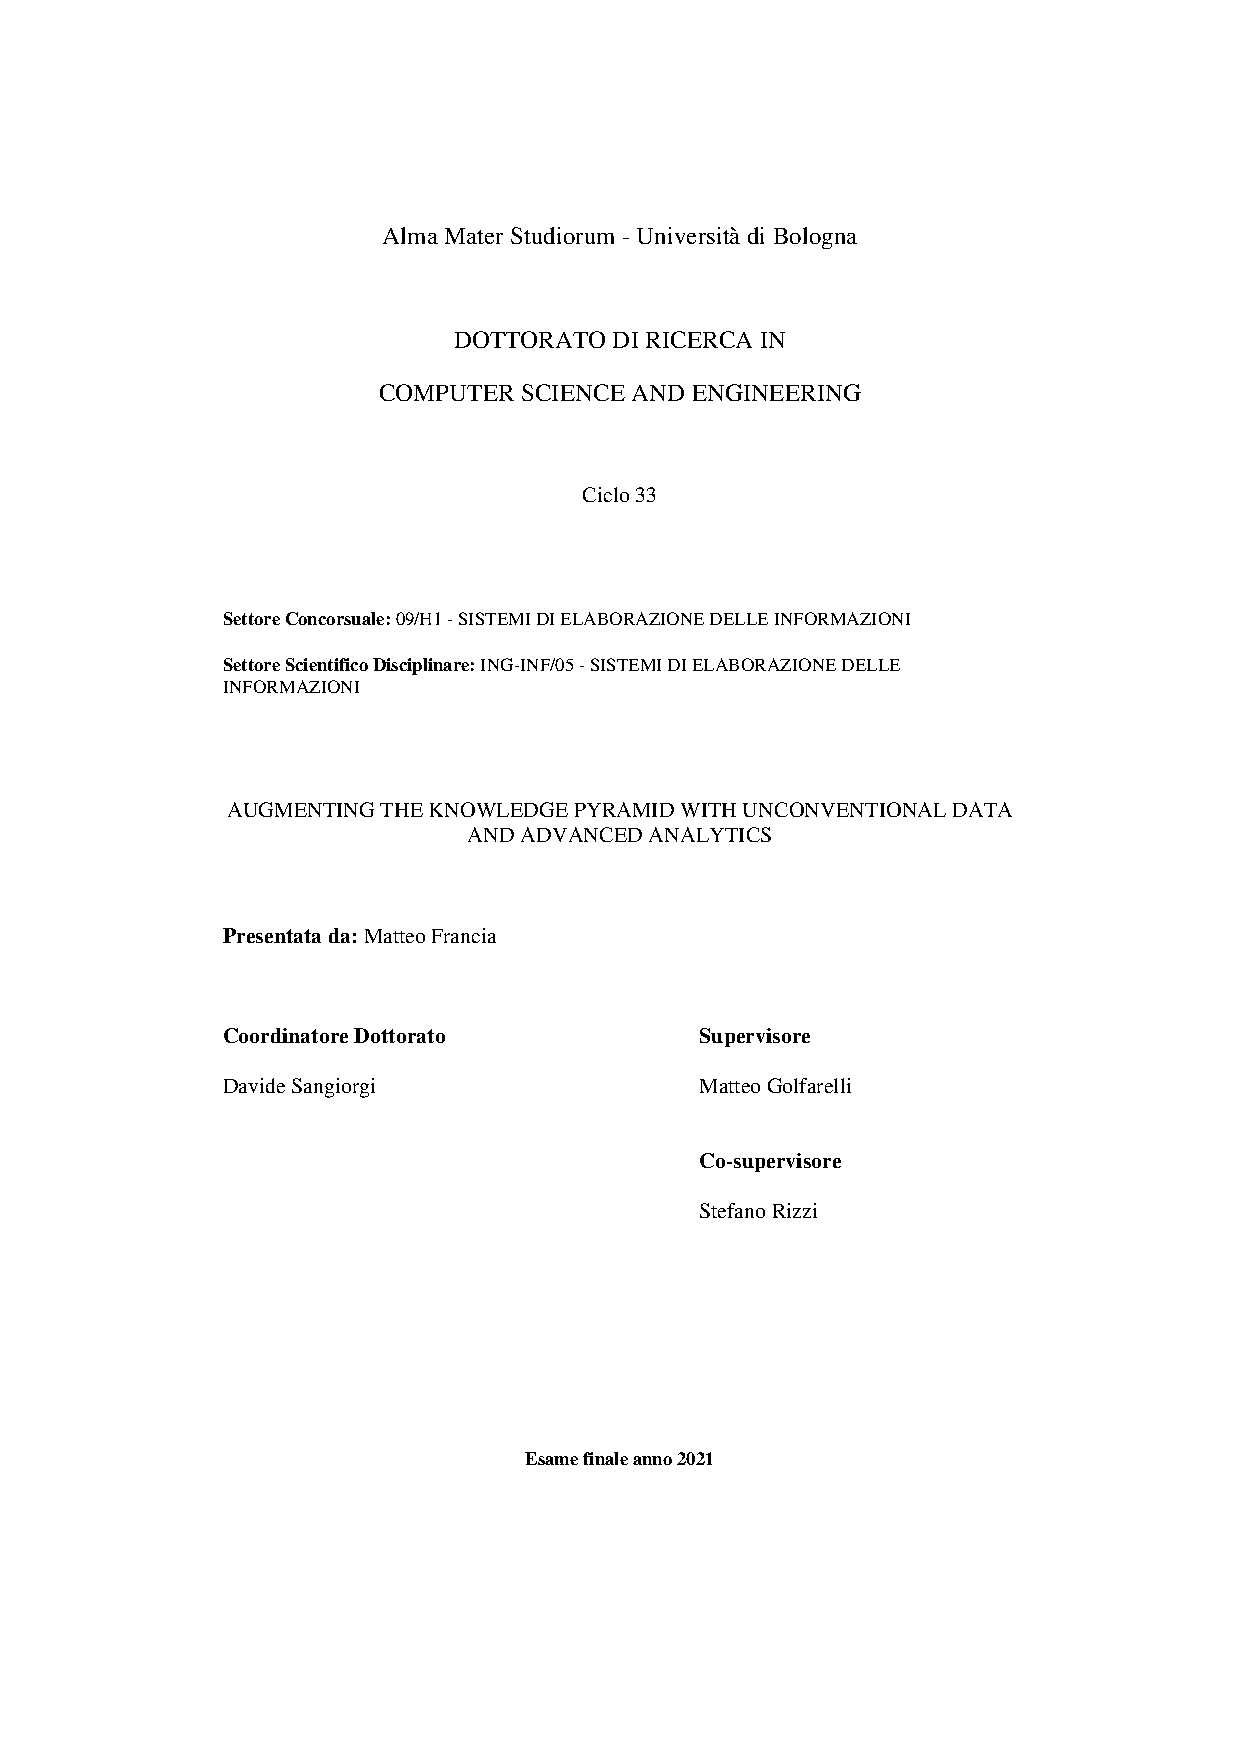
\includepdf[pages=-]{global/frontespizio.pdf}
\newpage
% 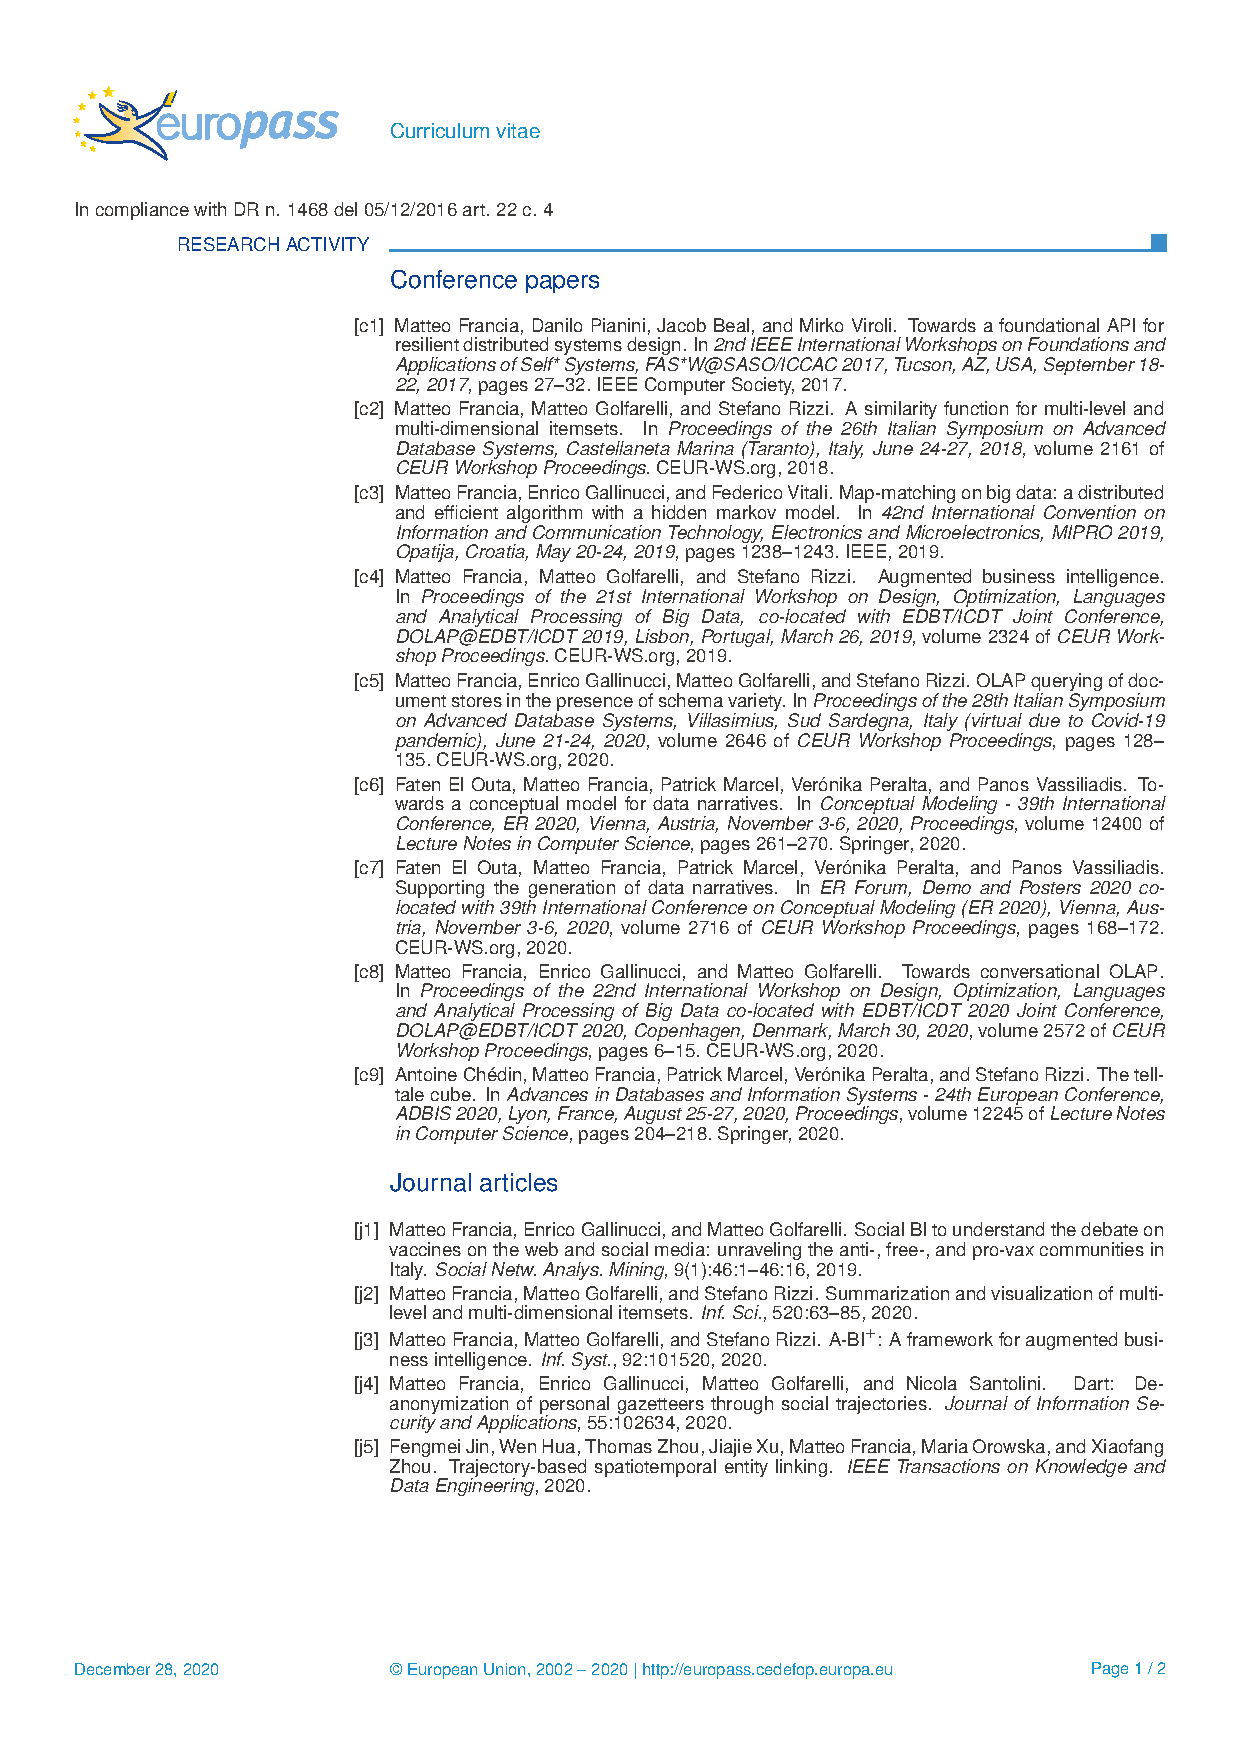
\includepdf[pages=-]{global/researchactivity.pdf}
% ******************************* Thesis Dedication ********************************
\begin{dedication}
\epigraph{\textit{
``A work of art is useless as a flower is useless.
A flower blossoms for its own joy.
We gain a moment of joy by looking at it.
That is all that is to be said about our relations to flowers.''\\
\vspace{0.5cm}
\textit{-- Oscar Wilde
% in a letter explaining ``All art is quite useless'', 1890
}}}{}
\vspace{30mm}
To Emilia.
\end{dedication}


% % ******************************* Thesis Declaration ***************************

\begin{declaration}
I hereby declare that except where specific reference is made to the work of 
others, the contents of this dissertation are original and have not been 
submitted in whole or in part for consideration for any other degree or 
qualification in this, or any other university. This dissertation is my own 
work and contains nothing which is the outcome of work done in collaboration 
with others, except as specified in the text and Acknowledgements. This 
dissertation contains fewer than 65,000 words including appendices, 
bibliography, footnotes, tables and equations and has fewer than 150 figures.
% Author and date will be inserted automatically from thesis.tex \author \degreedate
\end{declaration}
\include{global/quote}
\begin{acknowledgements}
\addcontentsline{toc}{chapter}{Acknowledgements}

Before diving into the depths of my research, I would like to acknowledge the sung and unsung heroes of this PhD journey.

\vspace{0.2cm}

% I would like to express my sincere gratitude to my advisors Prof. Matteo Golfarelli and Prof. Stefano Rizzi for their support and inspiration.
% My Ph.D. has been a joyful journey under their supervision.\\
The success of this thesis is certainly due to my research group, the business intelligence group (BIG).
First of all, I would like to thank my supervisor Prof. Matteo Golfarelli, who motivated me in the first place to start this PhD, and provided constant support and feedback.
I express my sincere gratitude to Prof. Stefano Rizzi for his priceless advice and encouragement.
I would like to thank my advisor Dr. Matteo Francia for his invaluable guidance, but also for welcoming me to the group ``so nicely''.
As to countless cups of coffee and \emph{italian passeggiate}, I thank my lab mates Dr. Enrico Gallinucci, Chiara Forresi, Manuele Pasini, Anna Giulia Leoni, Nicola Santolini, and Sterenn Roux.

\noindent At the Universitat Polit\`{e}cnica de Catalunya, Barcelona, huge thanks go to Prof. Alberto Abelló and Dr. Besim Bilalli for their inspiration and support during my Master's thesis, and throughout the whole PhD.

\noindent From Leibniz University, Hanover, I want to thank the AutoML group.
I would like to express my sincere gratitude to Prof. Marius Lindauer and Dr. Alexander Tornede, not only for the endless research insights and opportunities, but also for their kindness in welcoming me to the group.
Besides, I am grateful to have found an incredible group with which I had an amazing time.
I would like to thank Carolin Benjamins, Difan Deng, Theresa Eimer, Helena Graf, Aditya Mohan, Tim Ruhkopf, Sarah Segel, Daphne Theodorakopoulos, and Tanja Tornede.

\vspace{0.2cm}

With no doubts, I must thank my friends who both supported me during the ups and downs, and celebrated my achievements.
I would like to thank Gianluca Aguzzi,  Matteo Magnani, and Giuseppe Pisano.
I sincerely would not change anyone of you on this journey.
I would like to thank all the friends encountered during these years at the Cesena campus, especially in the Area 4.0 lab.
I believe the are not many groups having such a bond (and fun).
Especially, I would like to thank Giovanni Ciatto, Nicolas Farabegoli, Angela Cortecchia, Davide Domini, Matteo Magnini, Danilo Pianini, Martina Baiardi, Stefano Novellani, and Ruslan Shaiakhmetov.

\noindent My biggest thanks go to my mum Emilia for her never-ending support, solely a true \emph{mammone} can understand how much she means to me.
No less, I thank my father Renato and brother Yuri, for their continuous encouragement and for believing in me.

\noindent Last but not least, I would thank my partner Maria for cheering me up when ``it is not the day'', for her every-day caring, for all the fun, but -- mostly -- for always making me feel loved.

\end{acknowledgements}

\begin{abstract}
    \addcontentsline{toc}{chapter}{Abstract}

    % Riding the wave of recent groundbreaking achievements, artificial intelligence (AI) is currently the buzzword on everybody's lips and, building upon the notion of intelligence as learning, Machine Learning (ML) emerged as its pinnacle.
    % Riding the wave of recent groundbreaking achievements, artificial intelligence (AI) is currently the buzzword on everybody's lips and, addressing problems where human-crafted solutions are unfeasible, Machine Learning (ML) emerged as its pinnacle.
    % Artificial Intelligence (AI) stands as a transformative force, riding the wave of recent groundbreaking achievements, and Machine Learning (ML) emerged as its pinnacle, addressing problems where human-crafted algorithms are unfeasible and allowing algorithms to learn from historical data and discover solutions autonomously.
    % In particular, it addresses problems where human-crafted algorithms are unfeasible, allowing algorithms to learn from historical data and discover solutions autonomously.
    Riding the wave of recent groundbreaking achievements, artificial intelligence (AI) is currently the buzzword on everybody's lips and, allowing algorithms to learn from historical data, Machine Learning (ML) emerged as its pinnacle.
    The multitude of algorithms, each with unique strengths and weaknesses, highlights the absence of a universal solution and poses a challenging optimization problem.
    In response, automated machine learning (AutoML) navigates vast search spaces within minimal time constraints.
    By lowering entry barriers, AutoML emerged as promising the democratization of AI, yet facing some challenges.

    In \textbf{data-centric AI}, the discipline of systematically engineering data used to build an AI system, the challenge of configuring data pipelines is rather simple.
    We devise a methodology for building effective data pre-processing pipelines in supervised learning as well as a data-centric AutoML solution for unsupervised learning.

    In \textbf{human-centric AI}, many current AutoML tools were not built around the user but rather around algorithmic ideas, raising ethical and social bias concerns.
    % Motivated by such a mitigation call, this thesis contributes to human-centric AutoML, aiming at complementing, instead of replacing, human intelligence.
    We contribute by deploying AutoML tools aiming at complementing, instead of replacing, human intelligence.
    In particular, we provide solutions for single-objective and multi-objective optimization and showcase the challenges and potential of novel interfaces featuring large language models.

    Finally, there are application areas that rely on numerical simulators,
    % with domain experts manually configuring them through several trials and errors.
    often related to earth observations, they tend to be particularly high-impact and address important challenges such as climate change and crop life cycles.
    We commit to coupling these physical simulators with (Auto)ML solutions towards a \textbf{physics-coupled AI}.
    Specifically, in precision farming, we design a smart irrigation platform that: allows real-time monitoring of soil moisture, predicts future moisture values, and estimates water demand to schedule the irrigation.

    % starting from supervised and unsupervised learning. The former is provided with a ground
    % truth to drive the learning towards a user-specified objective function

    % for both supervised learnand unsupervised learning, a
    % towards a more human-centric AutoML process.
    % In particular,
    % This places a mitigation call a shift toward the human-centric paradigm
    % Enabling human intervention, translating into the need for a shift toward the human-centric paradigm.
    % pushed towards a more human-centric AutoML process aimed at complementing, instead of replacing, human intelligence.

\end{abstract}
\tableofcontents
% \listoffigures
% \listoftables
% \printnomenclature%[3em]

% ******************************** Main Matter *********************************
\mainmatter
\sloppy
% \chapter{The Knowledge Pyramid}
\begin{figure}[t]
    \centering
    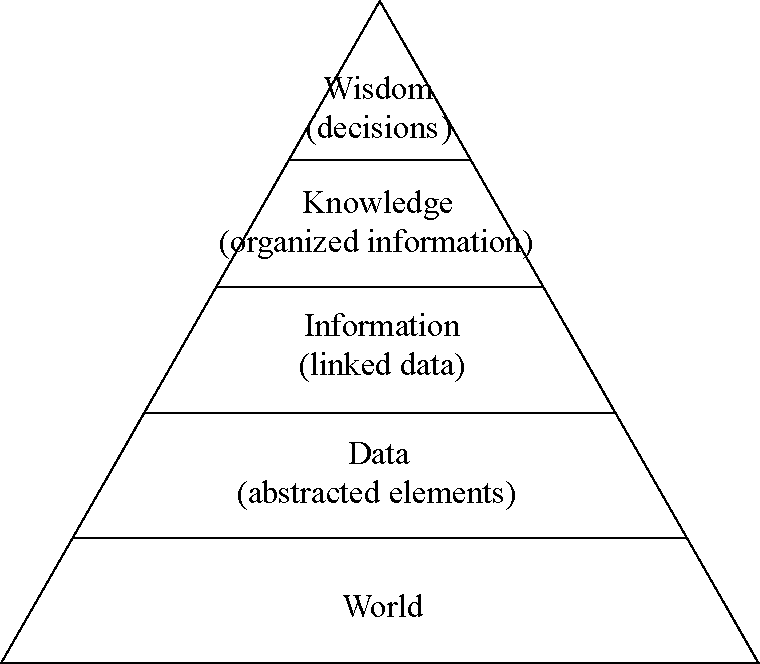
\includegraphics[scale=.7]{global/DIKW.pdf}
    \caption{The ``knowledge pyramid'' (also known as the ``Data Information Knowledge Wisdom pyramid'' or ``knowledge hierarchy''; adapted from \cite{DBLP:journals/oir/Stuart15b}).}
    \label{fig:dikw}
\end{figure}

Data science extracts actionable insights from raw data \cite{kelleher2018data}. The data transformation process is usually abstracted in the ``knowledge pyramid'' (also known as the ``Data Information Knowledge Wisdom pyramid'' or ``knowledge hierarchy''; \Cref{fig:dikw}), where data (i.e., symbols) are collected through measurements taken from the real world; information is processed and linked data that it is meaningful to scientists; knowledge is interpreted, understood, and organized information; and wisdom is knowledge in action. Climbing the pyramid is not a straightforward path and requires the iterative exploration and preparation of data so that patterns can be extracted, evaluated, and later deployed into models supporting effective decisions. 

Analytic applications strive to extract knowledge from data fueled by pervasive systems \cite{8423172}, where any device can be turned into a sensor leading to a huge volume and variety of available data \cite{vitali2021crop}. These \textit{unconventional}\footnote{We consider \textit{conventional} the data collected by operational databases, ERP (enterprise resource planning), and CRM (customer relationship management) enterprise systems} data (i.e., unstructured and non-relational data) have impacted on business intelligence (BI)---the discipline providing strategies and technologies to transform data into decision-making information---leading to BI 2.0, where decisions are drawn \textit{not only} on the data owned by the organization. Indeed, bigger data volumes lead to a holistic view of historic and current trends; higher data velocities ground decisions in continuously updated data, and broader data varieties provide many nuances of the matter at hand \cite{IBM4V}. On the one hand, volume and variety hinder the management, the integration, and the analysis of the collected data (from ``World'' to ``Data'' in \Cref{fig:dikw}), since each instance of unstructured data might have a different structure. This requires ad-hoc techniques for different data types (e.g., social networks \cite{DBLP:journals/snam/FranciaGG19} or sensor data \cite{DBLP:conf/mipro/FranciaGV19}). On the other hand, high availability has attracted scientists with no expertise in computer science or data engineering, requiring novel paradigms to support the ``Data''-to-``Knowledge''
%\footnote{Since ``wisdom'' is related to the \textit{application} of knowledge \cite{8423172}---besides no strict definition is given in the literature---we address the transformation of raw data into knowledge (i.e., patterns extracted with mining/machine learning models).} 
transformation with a higher abstraction level than formal programming languages (e.g., through graphical metaphors, recommender systems, or automatic transformation pipelines). Additionally, availability has enabled pervasive analyses, allowing data scientists to access data in hand-free contexts involving augmented reality and smart assistants.

While investigating these challenges, this thesis evolves into two parts.

\begin{figure}[t]
    \centering
    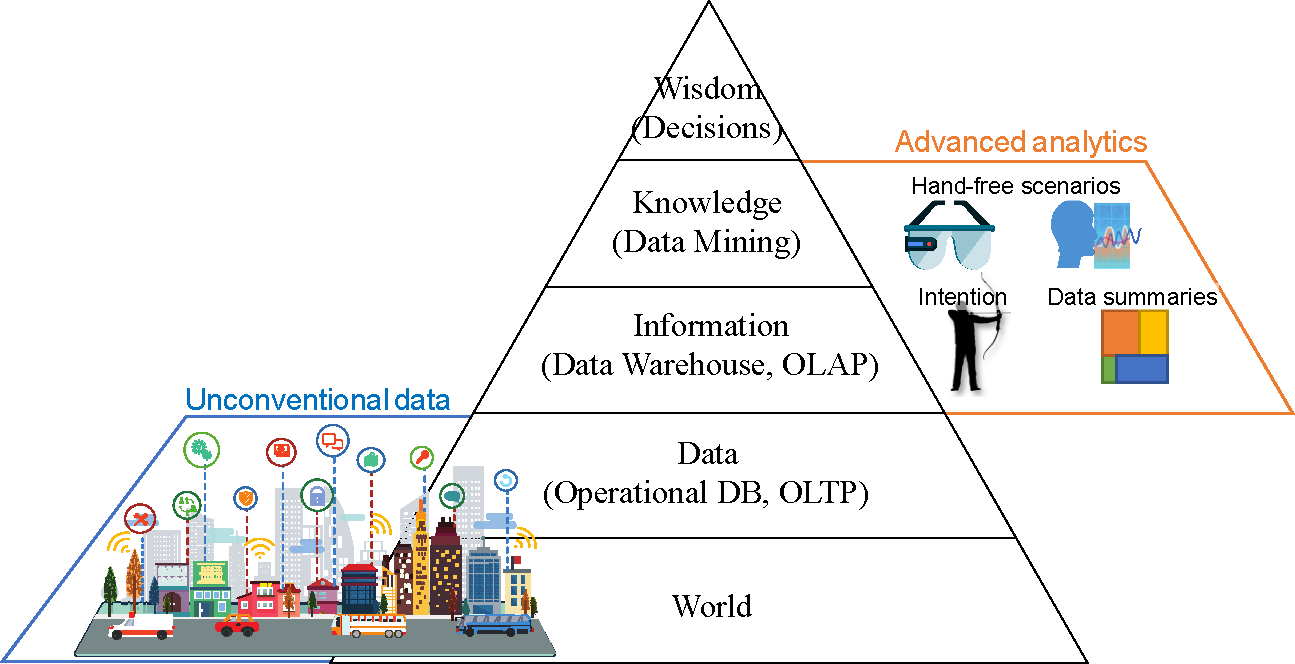
\includegraphics[scale=.65]{global/augmenting.pdf}
    \caption{Augmenting the knowledge pyramid with unconventional data (left) and advanced analytics (right).}
    \label{fig:aug}
\end{figure}

\paragraph{\Cref{part:trajectory}: Unconventional Data.}
Sensing provides real-time data upon which ``contextual'' decisions---ranging from user-centric to societal problems---are based. This includes data collected from human and technological assets (e.g., sensor or mobile networks), which are analyzed to monitor and manage urban and rural areas. Sensor data are highly available due to the growth of Internet of Things devices, have variable content, and their value comes from historic trends that range from hours to years \cite{kelleher2018data}. Such volume and variety demand for augmenting the knowledge pyramid with novel and scalable techniques for different data types (\Cref{fig:aug}). In urban mobility, spatiotemporal data (i.e., temporal sequences of spatial locations traced by moving objects and sampled through global or relative positioning sensors) are collected and processed for the sake of traffic analysis and forecasting, clustering of objects moving in similar paths, and habits profiling. Spatiotemporal data are challenging because of their uncertain, sparse, and multiresolution nature \cite{DBLP:journals/cacm/GilPBBBBCEGHHHK19}. Also, due to the number of moving objects (e.g., mobile devices, cars, taxis, and public transport in a metropolitan area) and to the sampling rate of positioning sensors (e.g., from minutes to seconds), mining mobility data easily scale up to big-data problems that require big-data solutions, hence introducing %a 
new business opportunities
% to analyze and extract information from data 
that were previously ignored because of technology limitations. Besides the valuable knowledge, due to high uniqueness \cite{DeMontjoye2013} and sensitivity (e.g., home and work locations), trajectory data expose individuals to privacy violations, demanding for ad-hoc techniques to (de-)anonymize historical trajectory datasets. In this direction, \Cref{part:trajectory} focuses on trajectory data and on the privacy implications of the publication of long-term mobility datasets.

\paragraph{\Cref{part:olap}: Advanced Analytics.}
Since the introduction of the relational model in the '70s, users used relational queries (e.g., SQL queries) to retrieve data collected in operational databases. This requires a good comprehension of programming languages and database management systems. Later, more user-friendly abstractions and tools provided a simpler view of the data, hiding the complexity of the underlying databases \cite{DBLP:journals/is/VassiliadisMR19} and transitioning from static (repetitive) workloads involving a few records (On-Line Transaction Processing, OLTP) to dynamic workloads (On-Line Analytical Processing, OLAP, and On-Line Analytical Mining, OLAM) involving a huge amount of records (\Cref{fig:aug}). The spread of data and analytical tools at hand has brought an increasing participation of data scientists with high competence in the business domain but low competence in computer science and data engineering \cite{DBLP:journals/is/VassiliadisMR19}. Indeed, data science emerged as an amalgamation of domain expertise with disciplines such as statistics, data mining, and databases \cite{vanderAalst2016}. Such amalgamation has brought challenges not only concerning big data volumes but also in terms of the increasing complexity and interdisciplinarity of the analytic questions. Enabling an effective participation in data science requires the investigation of user-centric paradigms supporting analytical querying and making knowledge extraction more accessible. Data scientists can benefit from proactive systems that ``understand'' the tasks at hand, make recommendations, and generate effective visualizations \cite{DBLP:journals/cacm/GilPBBBBCEGHHHK19}. For instance, in the digital twin scenario \cite{tao2018digital} where physical entities are mapped into a digital world, the synergy of personal assistants and augmented reality lacks analytic capabilities. Additionally, limited attention has been devoted to providing analytical reports that can be useful to let the user compare the current behavior of the visualized objects with their historical behavior. To this end, unconventional data sources, such as smart glasses and wearable devices, can be accessed by personal assistants (e.g., recommender systems) to address users' needs \cite{DBLP:conf/ictir/BahrainianC17}. Data scientists can interact with personal assistants through natural language interfaces which provide a higher abstraction level than formal queries and programming languages. In this direction, \Cref{part:olap} focuses on supporting data scientists with higher analytic abstractions than formal queries also in scenarios entailing pervasive data access. 

\chapter{Introduction}

Artificial intelligence (AI) is currently the buzzword on everybody's lips.
Riding the wave of recent groundbreaking achievements, from self-driving cars \citep{} to intelligent chatbots \citep{}, AI is transforming industries and reshaping our daily lives.
Several interpretations and definitions have been provided over the years, yet the seminal perspective given by the Turing test \citep{turing1980computing} is still one worth mentioning.
\begin{definition}[Artificial Intelligence \citep{turing1980computing}]
A machine that shows intelligence indistinguishable from that of human beings is qualified to be labeled as artificial intelligence.
\end{definition}
This translates into understanding what falls under the umbrella of \textit{intelligence}, which is defined differently across the research areas as reasoning, planning, and learning.

\begin{definition}[Machine Learning \citep{samuel2000some}]
A machine with the ability to learn without being explicitly programmed.
\end{definition}
Building upon the notion of intelligence as learning, i.e. Machine Learning (ML), emerged as the pinnacle of AI due to its disruptive advancements.
At its core, ML aims at addressing problems for which the development of algorithms by humans is not feasible, because the algorithm itself is either not known or cost-prohibitive.
Examples include face recognition, fraud detection, sale forecasting, and object ranking. 
The problems are solved instead by letting the algorithms (e.g., neural networks \cite{}) \textit{discover their own solutions}: they perform a training process atop a sample of historical data, borrowing techniques from disciplines such as numerical analysis, statistics, and information theory.
The training process consists of fitting internal parameters (e.g., weights and bias) and providing ML practitioners with a model, which is ready to ingest new data and tackle the problem at hand.

There exists a plethora of different algorithms solving the same problem with different strengths and weaknesses, confirming theoretical results proving that there is \textit{no silver bullet} \cite{kerschke2019automated}---no algorithm dominates all others in all respects.
Besides, algorithms often expose some hyperparameters controlling the learning behavior (e.g., learning rate). 
To unleash the full potential of ML, practitioners have to carefully tune such hyperparameters but get easily overwhelmed by the showcased problem of combined algorithm selection and hyperparameter (CASH) optimization.

Automated machine learning (AutoML) demonstrates to play a crucial role in this landscape by tackling the CASH problem and, going beyond, by handling ever-larger search spaces in surprisingly small time budgets \cite{}.
Remarkable milestones include bayesian optimization (BO) to explore promising configurations based on prior evaluations,
meta-learning (i.e., learning atop learning) to warm-start BO (i.e., to boost the convergence process) by suggesting configurations that worked well in previous similar cases, and multi-fidelity methods to partially evaluate time-consuming configurations.
Besides, off-the-shelf solutions \cite{} are provided to tune entire ML pipelines, achieving -- in some cases -- higher performance than experts.

By lowering the barrier of access, AutoML emerged as promising for democratization of AI, i.e. making it accessible to both experts and non-experts alike.
Yet, when it comes to real-case scenarios, the journey of learning is riddled with challenges, ranging from the need for human intervention to mitigate harnessing, to the need for physical simulators.
% and heterogeneity of the data to constraints that may apply to the problem, from need for domain knowledge to .
While \Cref{chap:background} provides the necessary background, the remaining of the thesis investigates these challenges evolving into two parts.




\paragraph{Part I: Human-centered AutoML}

The original promise of AutoML was to automate certain ML tasks to a significant extent, thereby democratizing it and enabling non-experts to apply it in their respective domains.
However, despite their success, many current AutoML tools were not built around the user but rather around algorithmic ideas.
The stacking of complex mechanisms on top of each other unavoidably led to a less understanding of the process by the user -- even ML experts -- and allowing for very limited interaction.
Parts of the community have hence pushed towards a more human-centered AutoML process aimed at complementing, instead of replacing, human intelligence.
% This becomes even more crucial nowadays
% Motivated by ethical concerns and social bias issues arising at each step of the ML process, this becomes imperative in such a mitigating call nowadays.
Besides, motivated by ethical concerns and social bias issues arising at each step of the ML process, this approach becomes even imperative in such a mitigating call nowadays.
By placing the user back in the loop, it would be possible to revise and supervise the entire process, ensuring fairness, transparency, and ethical compliance.

In this part, we focus on the following contributions.
\begin{itemize}
    \item Providing the AutoML formalization to explicitly deal with thorough pipelines i.e., concatenations of pre-processing transformations and ML algorithms.
    \item Devising human-centered solutions for the main categories of ML i.e., supervised and unsupervised learning. The former is provided with a ground truth to drive the learning towards a user-specified objective function, the latter is by nature exploratory -- does not benefit from any ground truth -- and optimizing an objective is even more challenging.
    \item Addressing multi-objective ML, i.e. optimization of more than one loss or objective function, by interactively learning user preferences and drive the optimization towards it.
    \item Showcasing potential challenges, opportunities, and risks of novel (human-centered) AutoML interfaces with large language models (LLMs), i.e. AI models trained on large corpora of text to understand and produce human-like answers.
\end{itemize}

We organize this part as follows.
\Cref{automl-chap:formalization} provides the comprehensive AutoML formalization for ML pipelines.
\Cref{automl-chap:supervised} and \Cref{automl-chap:unsupervised} address supervised and unsupervised learning respectively.
\Cref{automl-chap:moo} delves into multi-objective ML and, lastly, \Cref{automl-chap:llm} discusses the novel human-centered AutoML interfaces with LLMs.
% In this part, we devise human-centered AutoML solutions for the main categories of ML.
% While in \Cref{automl-chap:formalization} we provide the AutoML formalization to explicitly deal with thorough pipelines i.e., concatenations of pre-processing transformations and ML algorithms, \Cref{automl-chap:supervised} and \Cref{automl-chap:unsupervised} address supervised and unsupervised learning respectively.
% The former is provided with a ground truth to drive the learning towards a user-specified objective function, the latter is by nature exploratory -- does not benefit from any ground truth -- and optimizing an objective is even more challenging.
% Then, \Cref{automl-chap:moo} delves into multi-objective ML, i.e. optimization of more than one loss or objective function.
% Lastly, \Cref{automl-chap:llm} showcases the potential challenges, opportunities, and risks of novel (human-centered) AutoML interfaces with large language models, i.e. AI models trained on large corpora of text to understand and produce human-like answers.

\paragraph{Part II: Physics-coupled AutoML}

As application areas go, there are domains in which ML models are not yet widespread.
Usually related to earth observations, the deployed applications tend to be particularly high-impact, trying to mitigate challenges such as climate change by delivering (more) eco-friendly systems.
Examples include weather forecasts and crop life-cycle management.
Domain experts leverage their knowledge to tune numerical simulators -- which encode well-known physical laws -- and deliver forecasts and analyses.
However, this process faces several challenges.
% several issues jeopardize this process.
The non-existence of universal well-defined practices translates to several trials and errors, with domain experts manually configuring the simulator parameters until an acceptable solution is found.
Yet, as variables involved in physics phenomena are subject to constant change, such numerical solution must undergo periodic (re-)calibration.
Besides, with the torrent of remotely sensed data available today, opportunities to integrate real-time observations in predictive models have emerged that traditional methods are not equipped to handle.
This is where advances in AI can push forward to enhance our understanding, provide support and, if necessary, steer the course of resolving global concerns to a more favorable future.
For instance, ML models exhibit singular performance in adapting themselves to handle scenarios different from the one they were trained on (e.g., fine-tuning of network parameters) and AutoML can significantly impact in automating several stages (e.g., tuning simulators and ML models).
% At the same time, relying on fully-automated data-driven methods for problems as complex and impactful as these is doomed to result in biased and unreliable.
% This underscores the ongoing importance of domain experts in this endeavor, highlighting their crucial role, with AI serving as a powerful tool.
% This is why domain experts, as always, remain crucial in this process, and why AI should be there as a powerful tool that supports them in fully taking advantage of the new opportunities we are presented with.

In this part, we focus on precision farming, which plays a pivotal role in addressing water wastage and improving crop efficiency.
\Cref{precision-chap:background} provides the necessary background and formalization in precision farming.
\Cref{precision-chap:architecture} overviews the architecture of our big-data smart-irrigation platform.
\Cref{precision-chap:orchard} deepens on Orchard3D-Lab, a well-known crop and soil simulator enhanced with auto-tuning and data assimilation capabilities, i.e. ingestion of sensor data for more reliable estimations.
\Cref{precision-chap:pluto} and \Cref{precision-chap:forecasting} delve -- respectively -- into the modules of real-time soil moisture monitoring and forecasting.
Finally, \Cref{precision-chap:smart-irrigation} deepens the smart-irrigation algorithm.


\chapter{Background}
\label{chap:background}

Alan Turing defines the field of AI in cognitive terms \cite{turing1980computing}, raising the question of whether machines can show intelligence, and along this line Arthur Samuel defines ML \cite{samuel2000some}, building upon the notion of intelligence as learning.
A more formal definition is provided by Tom M. Mitchell \citep{mitchell1997machine}, who delineates the behavior of algorithms studied in machine learning and introduces the concepts of \textit{task} and \textit{experience}.
\begin{definition}[Machine Learning \citep{mitchell1997machine}]
    A computer program is said to learn in some class of tasks, with respect to a performance measure, if its performance improves with experience.
\end{definition}
Notably, the formalization of experience is contingent upon the task to address, which is crucial because determines what the ML algorithm can observe and, in turn, how it operates.
Specifically, the literature identifies three different ML tasks: \textit{supervised}, \textit{unsupervised}, and \textit{reinforcement learning}.

\paragraph{Supervised learning} This is the kind of learning studied in most current research in the ML field. The algorithm is provided with a sample of data describing scenarios that have been \textit{experienced} in the past along with the corresponding \textit{ground truth}---i.e., values that indicate the correct outcomes.
The goal consists of finding a \textit{function} that maps samples to outcomes so that the next unseen scenarios can be labeled correctly.
Besides, according to the nature of such data, the literature makes the following distinctions.
\begin{itemize}
    \item \textbf{Classification} tasks, when the outcome can assume finite values and it represents the class to which the instances belong e.g., in an image recognition use-case: ``dog'', ``cat'', ``car'', or ``tree''.
    \item \textbf{Regression} tasks, when the outcome is continuous e.g., predicting house prices, stock prices, or temperature.
\end{itemize}

\paragraph{Unupervised learning}
Here, the samples come with no ground truth available.
The algorithm has to guess the outcome by uncovering hidden insights or patterns, investigating different partitionings, or estimating density distributions within the data.
Analogously, tasks can be further categorized.
\begin{itemize}
    \item \textbf{Clustering} or \textbf{cluster analysis} tasks, when the outcome can assume finite values and it refers to the group that better represents the instances e.g., identifying customer segments based on purchasing behavior.
    \item Otherwise, the nomenclature usually comes after the task semantic e.g., anomaly detection assigns an outlier score to each instance that deviates from the overall distribution.
\end{itemize}
% Unsupervised tasks are inherently exploratory in nature and are often employed in data mining to provide explanations for the given scenarios or even to summarize them.

\paragraph{Reinforcement Learning} Standing on the edge of the ML landscape, it has been categorized as the learning that differentiates the most from ``classical'' tasks \cite{sutton2018reinforcement}.
Here the experience is not sampled and fed to the algorithm but rather comes from interactions with an environment.
The algorithm learns by making decisions and receiving feedback based on its actions, allowing it to adapt its behavior over time.\\

%TODO: Qua c'è da menzionare che infatti automatizzare RL, in letteratura, prende il nome di AutoRL mentre noi facciamo AutoML.
This thesis focuses on supervised and unsupervised learning.
% providing a formalization that covers both cases.
Particularly in this chapter, \Cref{automl-background-sec:ml} introduces the building blocks such as dataset, algorithm, and hyperparameter; while
% provides the necessary background in ML,
\Cref{automl-background-sec:automl} formalizes the problems tackled by automated machine learning (AutoML), up to the combined algorithm selection and hyperparameter optimization.
% along with the state-of-the-art techniques to solve them.
% and finally \Cref{automl-background-sec:formalization} extends the formalization towards a more operational level of ML, enabling the user to handle comprehensive ML pipelines---i.e., concatenations of steps that cover more than the sole learning process.
% Here we can also put something like " ... extends the formalization focusing on a more operational level of ML and methods that following this way enables to handle comprehensive ... "

\section{Machine Learning}\label{automl-background-sec:ml}

At the core of each and every task lies the data, serving as the essential fuel for the learning process because providing the means to observe the real world.
Specifically in ML, we refer to a dataset $\altmathcal{D}$ as a sample of data from which it is possible to learn that experience of interest.

\begin{definition}[Dataset]\label{def:dataset}
    A \textit{dataset} $\altmathcal{D}$ is a collection of data points $X$, with corresponding space $\altmathcal{X}$.
    According to the task $T$, the dataset may include the ground truth $Y$ within its corresponding space $\altmathcal{Y}$ (supervised) or not (unsupervised).
    \begin{equation*}\label{eq:dataset}
        \altmathcal{D} = \left\lbrace\,
        \begin{array}{@{}l@{}l@{\quad}l@{}}
            (\pmb{x}_i, y_i)_{i=1}^N & \in \mathbb{D} \subset \altmathcal{X} \times \altmathcal{Y} & \text{{if }} T = \text{{supervised}} \\
            (\pmb{x}_i)_{i=1}^N & \in \mathbb{D} \subset \altmathcal{X} & \text{{if }} T = \text{{unsupervised}}
        \end{array}
        \right.
    \end{equation*}
\end{definition}

Intuitively, a dataset resembles a structured table where each row represents a unique instance $x \in X$ characterized by specific features in their domain $\altmathcal{X}$.
The features, denoted by the columns, describe the diverse factors or characteristics influencing a particular outcome $Y$ in its domain $\altmathcal{Y}$.
While in supervised learning the ground truth is provided with the aim of understanding the hidden relationships between features and corresponding outcomes, in supervised tasks, the most appropriate outcome has to be found by discovering patterns within the data.

\begin{example}[Iris dataset \cite{iris}]
    The iris dataset contains $150$ instances of flowers ($X$) under four features in cm ($\altmathcal{X} \subset \mathbb{R}^4$): sepal length, sepal width, petal length, and petal width.
    The data have been collected to quantify the morphologic variation within the Iris species ($Y$), which can assume the following $3$ classes ($\altmathcal{Y}$): Iris setosa, Iris virginica and Iris versicolor.
    \begin{table}[!h]
        \centering
        \begin{tabular}{llll|l}
            \hline
            Sepal length & Sepal width & Petal length & Petal width & Class \\ \hline
            % $5.1$ & $3.5$ & $1.4$ & $0.2$ & Iris-setosa \\
            $4.9$ & $3.0$ & $1.4$ & $0.2$ & Iris-setosa \\
            % $7.0$ & $3.2$ & $4.7$ & $1.4$ & Iris-versicolor \\
            $6.4$ & $3.2$ & $4.5$ & $1.5$ & Iris-versicolor \\
            % $6.3$ & $3.3$ & $6.0$ & $2.5$ & Iris-virginica \\
            $5.8$ & $2.7$ & $5.1$ & $1.9$ & Iris-virginica \\ \hline
            \
        \end{tabular}
        \caption{Example tuples from the Iris dataset.}
        \label{tbl:iris}
    \end{table}
    This dataset is also used in unsupervised learning tasks by discarding the class attribute, yet the data only contains two clusters with rather obvious separation.
\end{example}

% The aim is to discover the hidden relationships between inputs $X$ and outputs $Y$, hence learning a function $f: \altmathcal{X} \rightarrow \altmathcal{Y}$.
Despite the task, the ultimate goal is learning a function $f: \altmathcal{X} \rightarrow \altmathcal{Y}$. A (machine) learning \textit{algorithm} $A$ leverages data points in $\altmathcal{D}$ to estimate such a function $f$, which is expressed via a vector of \textit{model parameters} $H$.
Most algorithms further expose hyperparameters $\lambda_1, \dots, \lambda_K$ that change the functioning of the algorithm itself.

\begin{definition}[Machine Learning Algorithm]\label{def:algorithm}
    Given a dataset $\altmathcal{D}$ and a hyperparameter space $\pmb{\Lambda}$, an algorithm $A$ provides a model $H$ from the model space $\altmathcal{H}$.
    \begin{equation*}\label{eq:algorithm}
        A: \mathbb{D} \times \pmb{\Lambda} \rightarrow \altmathcal{H}
    \end{equation*}
    Given the hyperparameters $\lambda_1, \dots, \lambda_M$, with corresponding spaces $\Lambda_1, \dots, \Lambda_M$, we refer with $\pmb{\lambda}$ to a hyperpaprameter configuration sampled from the space $\pmb{\Lambda} = \Lambda_1 \times \dots \times \Lambda_M$.
\end{definition}

Popular learning algorithms include, for supervised tasks: decision trees \cite{} and neural networks \cite{}; for unsupervised tasks: k-means \cite{} and isolation forest \cite{}.

\begin{example}[Decision Tree]
    The decision tree algorithm recursively splits instances based on their feature values, creating a hierarchical tree-like structure where each leaf represents a class.
    Notably, in its supervised nature, the tree can be built by minimizing the entropy of the leaves.
    Hyperparameters such as the maximum depth of the tree or the minimum number of instances in the leaves control the complexity and structure of the resulting tree.
\end{example}

\begin{example}[K-Means]
    The k-means algorithm aims to partition the instances into a predetermined number of clusters based on their feature similarity.
    Being unsupervised, the algorithm iteratively assigns instances to clusters and updates the cluster centroids until its convergence criteria i.e., instances in the same cluster are more similar than instances in a different cluster.
    Hyperparameters such as the number of clusters and the similarity measure affect the returned partitioning.
\end{example}

Sticking with the decision tree algorithm as an example, a deeper tree with more splits may capture intricate patterns but is prone to \textit{overfitting} i.e., the model fits the data too closely and performs poorly on new, unseen data.
On the other hand, a shallower tree might generalize better but may overlook finer details.
For such reasons, we need loss functions that assess the quality of hyperparameter configurations.

\begin{definition}[Loss Function]\label{def:loss}
    Given a dataset $\altmathcal{D}$ and a model $H$, the loss function $\altmathcal{L}$ quantifies how well the given model performs on $\altmathcal{D}$.
    \begin{equation*}\label{eq:loss}
        \altmathcal{L}: \altmathcal{H} \times \mathbb{D} \rightarrow \mathbb{R}
    \end{equation*}
    The term loss typically refers to the error, hence the lower the better; instead, when higher values are favored, we refer to quality metrics.
\end{definition}

Not only loss functions are inevitably built specifically for the task at hand but, in supervised learning, their application should also follow protocols that assure the consistency and reliability of the estimated model performance.
In particular, since the model is built by leveraging the ground truth of the data(i.e., model training), we need to evaluate its performance on different data to not overestimate the generalization capacity (i.e., model validation).
Indeed, the loss function is applied by splitting the original dataset $\altmathcal{D}$ into two disjoint datasets $\altmathcal{D}_\mathit{train}$ and $\altmathcal{D}_\mathit{valid}$, where the model is trained only based on $\altmathcal{D}_\mathit{train}$ but validated with $\altmathcal{L}$ on $\altmathcal{D}_\mathit{valid}$.

\begin{example}[Misclassification Error]
    Given the validation set $(x, y) \in D_\mathit{valid}$  and the model $H$ resulted from the training $A(D_\mathit{train}, \lambda)$, then the loss MIS computes the fraction of incorrect predictions made by $H$.
    \begin{equation*}
        MIS(H, \altmathcal{D}_\mathit{valid}) = \frac{1}{|D_\mathit{valid}|}~\mathlarger{\sum}_{(x, y) \in D_\mathit{valid}} (H(x) \ne y)
    \end{equation*}
    In classification tasks, the accuracy ($ACC = 1 - MIS$) is often used as a quality metric.
\end{example}

Both model training and validation demand substantial amounts of data to -- respectively -- build and assess the model's performance with statistical relevance.
A practical solution is the $k$-fold cross-validation technique.
This divides the dataset into $k$ folds and, for each fold, uses the corresponding subset of data for testing while employing the remaining $(k - 1)$ folds for training.

\begin{definition}[$K$-Fold Cross-Validation]
    The $k$-fold cross-validation provides a protocol to validate an algorithm $A$ with corresponding hyperparameter configuration $\lambda$ via a loss $\altmathcal{L}$ on a dataset $\altmathcal{D}$.
    \begin{equation*}
        \frac{1}{k}~\mathlarger{\sum}_{i=1}^{k} \altmathcal{L}(A(\altmathcal{D}_{train}^{(i)}, \lambda), \altmathcal{D}_{valid}^{(i)})
    \end{equation*}
    where $\altmathcal{D}_{train}^{(i)} = \altmathcal{D} \setminus \altmathcal{D}_{valid}^{(i)}$.
\end{definition}

When it comes to unsupervised learning

\section{Automated Machine Learning}\label{automl-background-sec:automl}


% \begin{itemize}
%     \item Qui ci va sicuramente la formalizzazione
%     \item la motivation è dubbia, forse ripeteremmo quello che è scritto sopra nell'Introduction
% \end{itemize}



\part{Human-centered AutoML}\label{part:automl}


\chapter{Formalization}\label{automl-chap:formalization}

% 
\chapter{Effective Data-preprocessing Pipelines in Supervised Learning}
\label{data-centric-chap:supervised}

\begin{figure*}[t]
    \centering
    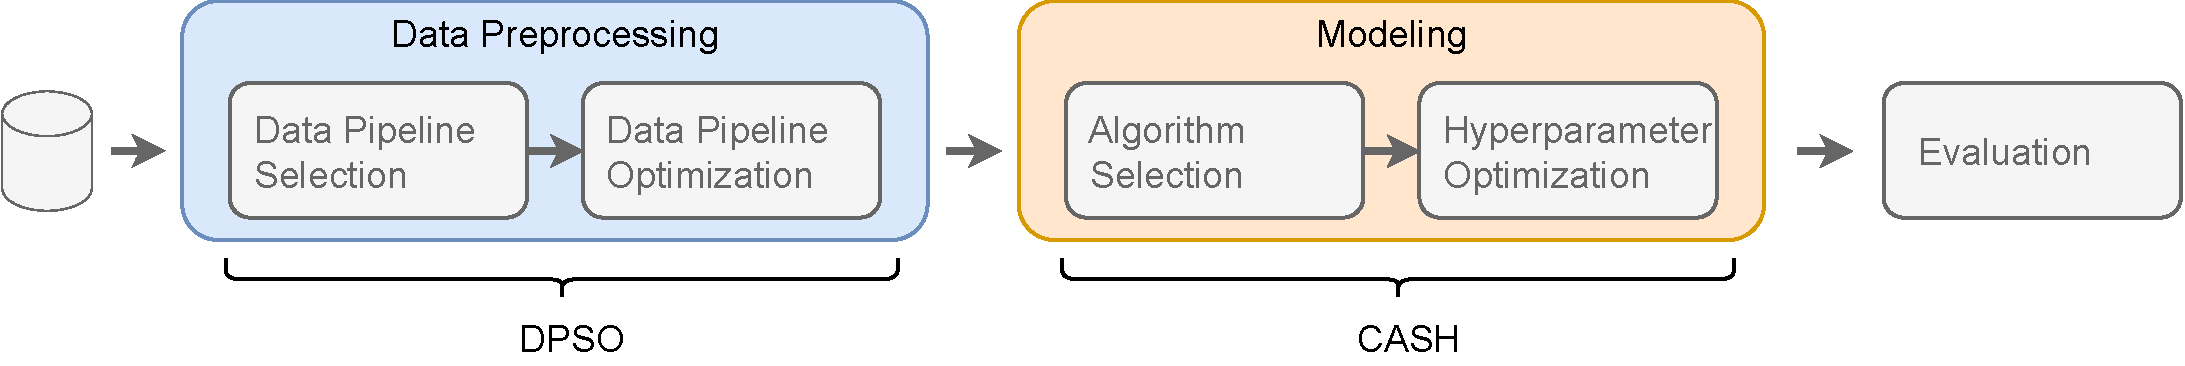
\includegraphics[width=1.0\textwidth]{chapters/data-centric/supervised/img/data-analytics-pipeline.pdf}
    \caption{Data analytics pipeline generation in a knowledge discovery process.}
    \label{effective-fig:data-analytics-pipeline}
\end{figure*}

To unleash the full potential of ML, data-centric AI focuses on shaping data according to the task and algorithm at hand.
With reference to the CRISP-DM process model,  \Cref{effective-fig:data-analytics-pipeline} summarizes the stages involved and the corresponding problems in the literature.
Firstly, data are extracted in a raw format from different sources and sifted out so that only a relevant subset is selected.
Next, during the pre-processing stage, the data pipeline selection and optimization (DPSO) \cite{Quemy19DOLAP} problem is tackled.
Once the data is transformed into the proper form, the modelling stage focuses on the combined algorithm selection and hyperparameter (CASH) optimization problem.
Finally, pipelines and algorithms
are evaluated over the dataset until an acceptable result is obtained.

It is well-known that the whole process requires expertise and is particularly challenging.
Particularly, data scientists spend most of their time on the heavily laborious work of pre-processing (i.e., around 50-80\% of the total \cite{Munson09Pre}).
Some AutoML frameworks \cite{auto_sklearn, mohr2018ml}, mix-in pre-processing during modelling optimization, but typically include very few transformations or do not consider all the necessary steps (e.g., imputation, rebalancing), thus in a way overlooking it.
Inspired from \cite{Munoz09DOLAP}, we contend that there is need for more data-centric techniques, encompassing all the steps of data pre-processing \cite{Vaisman14Book}.
Assistance is required in every phase \cite{Bilalli16IOTBD}.
By considering pre-processing as an integral component of the learning process, and carefully selecting and optimizing data pipelines, it is easy to obtain results that go beyond the ones obtained by only optimizing ML algorithms.

To briefly illustrate this, we perform an experiment on the well known \texttt{bank-marketing}\footnote{\url{https://archive.ics.uci.edu/ml/datasets/Bank+Marketing}} dataset, using HyperOpt \cite{HyperOptICML13} as an AutoML approach to optimize the parameters of three different ML algorithms, namely Naive Bayes (NB), K-Nearest Neighbor (KNN), and Random Forest (RF).
We provide an initial budget of 50 iterations for optimizing the hyperparameters of the algorithms, and after the 50th iteration, we fix the algorithm configuration to the best one achieved so far and start optimizing the pre-processing pipeline\footnote{This order is used only for the sake of illustration.}.
In \Cref{effective-fig:pre-processing-impact}, the ratio of the change in terms of accuracy (i.e., obtained after the i-th iteration to the baseline/default accuracy) is plotted against the number of different configurations visited by HyperOpt (i.e., iterations).
Observe that after the 11th iteration for NB and KNN, and after the 26th iteration for RF, the lines remain flat.
That is, from there on, no improvement is achieved by optimizing the hyperparameters of the algorithms until the 50th iteration is reached. At this point, a sudden jump is observed and the results start to improve again, going clearly beyond the ones obtained before, thanks to the optimizations performed now over the pre-processing pipeline.

\begin{figure}[t]
    \centering
    \includegraphics[width=0.7\textwidth]{chapters/data-centric/supervised/img/pre-processing-impact.pdf}
    \caption{Evolution of accuracy during the optimization process. The first 50 configurations optimize only the hyperparameters and after the 50th configuration, the pre-processing pipeline is optimized instead.}
    \label{effective-fig:pre-processing-impact}
\end{figure}

\paragraph{Challenges} Including pre-processing in the learning process heavily increases the search space, making the problem much harder.
DPSO entails two challenges that the data scientists have to undergo to find the most appropriate pipeline: (i) choose how to order the different pre-processing steps  (i.e., pipeline selection), and (ii) choose which transformations, with corresponding hyperparameters, should be adopted in the final implementation  (i.e., pipeline optimization).
To better distinguish between pipeline selection and its optimization, we follow the notation from \cite{Quemy20InfSystems}: a \textit{prototype} is the fixed and ordered sequence of pre-processing steps, its optimized instantiation of each transformation (with their hyperparameters) is known as \textit{executable pipeline}.

\paragraph{Contributions} The aim of this chapter is to study the two questions raised and propose a method for selecting effective pre-processing prototypes that, once optimized through some optimization technique (e.g., Bayesian optimization), improve the final result of the analysis.
To keep discussions and experiments simpler, we stick to supervised learning tasks.
The main contributions can be summarized as follows.
\begin{itemize}
    \item We empirically evaluate the impact of optimizing the exhaustive set of potential prototypes and find out that	there is no universal solution---i.e., prototype that works best for each dataset and algorithm considered.
    \item We define a method that given an ML algorithm and a set of pre-processing steps, is capable of generating the right order, obtaining effective pre-processing prototypes that are then instantiated via bayesian optimization.
    \item We suggest a meta-learning step (i.e., learning on top of learning) where the relationships between pre-processing transformations and dataset characteristics are learned in order to create rules that help with the initial instantiation of the prototypes.

	We exemplify our meta-learning study generating simple but not obvious and effective rules for two kinds of pre-processing steps, namely, Feature Engineering and Rebalancing.
    \item We perform a comprehensive evaluation by comparing the performance of optimizing prototypes generated following our method, and find out that:
    \begin{enumerate}
        \item with 24 times less time budget, our proposed pipelines obtain results whose median is above 90\% of the ones generated via exhaustive search.
        \item on average, in 73\% of the cases, splitting evenly the time budget between pre-processing and modelling outperforms the results of solely optimizing the latter.
    \end{enumerate}
	\item We deploy \textbf{AutoPrep}, a reproducibility framework for the automatic generation of effective pre-processing pipeline prototypes. Specifically, in \cite{giovanelli2023reproducible}, we introduce: (i) a detailed reproducibility protocol, (ii) software, and (iii) datasets in a self-contained environment.
	The experiments were run on several machines and confirmed all the inishts in this chapter.
\end{itemize}

The remaining of this chapter is organized as follows:
\Cref{effective-sec:related-work} discusses the related work,
\Cref{effective-sec:methodology} presents our method of generating effective pipelines,
\Cref{effective-sec:evaluation} provides an extensive evaluation of the pipelines created using our proposed method and, finally, \Cref{effective-sec:conclusions} provides the conclusions and future work.


\section{Related Works}
\label{effective-sec:related-work}
At the beginning, the AutoML community followed the AI trend of contributing under a more algorithmic perspective, focusing on modelling---i.e., the resolution of the CASH problem.
Recently however, the direction has shifted towards designing systems that additionally or specifically provide user assistance in the data pre-processing step---i.e., solving the DPSO problem.
We can categorize works according to the optimization policy \cite{quemy2019data} they adopt.
On the one hand, some automate data pre-processing via split-like policies---i.e., addressing DPSO in isolation from CASH (\Cref{effective-ssec:dpso}).
On the other hand, some consider optimizing DPSO along with CASH, adopting a joint policy---data pre-processing in synergy with modelling (\Cref{effective-ssec:dpso-cash}).

\subsection{Optimization with Split-like Policies}
\label{effective-ssec:dpso}

In \cite{Quemy20InfSystems}, authors demonstrate the impact of optimizing the pre-processing pipelines, but considering only a single fixed prototype and only a few datasets.
However, as we have already seen (\Cref{effective-sec:eval-universal-pipeline}), a single fixed prototype cannot perform best for every dataset.

In PRESISTANT \cite{presistant18CSI,presistant18CAISE,presistant19DKE}, authors tackled the problem of recommending pre-processing transformations to non-expert users.
They identify the pre-processing transformations and rank them in advance, based on their potential impact to the final analysis.
However, they do not consider pre-processing pipelines, but only single transformations, expecting that the analyst applies the process iteratively.

In ActiveClean \cite{ActiveClean16PVLDB}, authors define a method that aims at prioritizing the cleaning of records that are more likely to affect the results of the analysis, assuming that the latter belongs to the class of convex loss models (i.e., linear regression and SVMs).
Hence, instead of recommending the transformations to be applied, the system recommends the subset of data that needs to be cleaned at a given point.
The type of pre-processing to be applied is left to the user, assuming that the user is an expert.

In Learn2Clean \cite{Berti19WWW}, based on a reinforcement learning technique, for a given dataset and an ML model, an optimal sequence of pre-processing transformations is generated so that the quality of the ML model is maximized.
Yet, similarly to \cite{Quemy20InfSystems}, the pipeline prototype is fixed in advance.

In Alpine Meadow \cite{Shang19SIGMOD}, authors follow a similar approach to ours in that they define two steps for the pre-processing phase. One, the so-called \textit{logical pipeline plan}, which is roughly equivalent to the \textit{prototype} defined in this work, and the second the \textit{physical pipeline plan} which translates to \textit{executable pipelines} used in this work.
The physical plan is generated through a combination of Bayesian optimization, meta-learning, and multi-armed bandits.
For the logical plans, they rely on rules but without clear evidence on how they are generated.
Moreover, it is not clear whether the logical plan is fixed as in \cite{Quemy20InfSystems} and if some further adjustment from the user is required.

\subsection{Optimization with a Joint Policy}
\label{effective-ssec:dpso-cash}
Auto-sklearn \cite{Feurer15AutoSklearn} is based on the popular Python library scikit-learn.
The authors, inspired by Auto-Weka, address the problem with the Sequential Model-based Algorithm Configuration (SMAC).
Furthermore, they improve the approach by adding a meta-learning phase (i.e., learning on top of learning) at the beginning and an ensemble technique at the end.
Meta-learning leverages previous ML experiments and learns promising configurations to warm-start (i.e., boost the convergence) the Bayesian Optimization.
Ensemble techniques merge predictions from multiple ML models to statistically outperform the base models.
Yet, they consider a small set of transformations and also consider a single fixed prototype.

TPOT \cite{Olson16Tpot} is a tree-based pipeline optimization tool using genetic programming while requiring little to no expertise from the user.
In TPOT however, they only consider one transformation inside the optimization process (i.e., Feature Engineering).

ML-Plan \cite{mohr2018ml} uses hierarchical planning, a particular form of AI planning, to propose a solution to both the pre-processing and the modeling phases.
As in context-free grammars, there are complex tasks (non-terminal symbols) that are derived as long as primitive tasks (terminal symbols) are not obtained.
Typically, standard graph search algorithms (e.g., depth-first search, best-first search, etc.) are employed to solve such problems.
ML-Plan successively creates solutions in a global search instead of changing given solutions in a local search. However, due to the problem constraints, they adopt a randomized best-first search, randomly choosing the solution path.

AutoBazaar \cite{AutoBazaar} is a Python open-source tool.
Like in ML-Plan \cite{mohr2018ml}, both pre-processing and modeling phases are covered.
Here the last step of a prototype is the machine learning algorithm.
The approach involves two different steps.
Firstly, a \textit{catalog} proposes a collection of prototypes (with an ML algorithm as last step) based on the task and the dataset itself.
Secondly, the optimization process starts tuning the prototypes until either the time budget is expired or the prototypes are all optimized.
In particular, a \textit{selector} and a \textit{tuner} work in synergy.
The former decides which prototype should be optimized next.
Such a task is treated as a multi-armed bandit problem.
As to the tuner, bayesian optimization is chosen.
At the end, the prototype that achieved the higher accuracy is elected.
However, AutoBazaar strictly depends on the catalog.
Such a component memorizes all the possible primitives and supported tasks.
The prototypes are hard-coded for each task.
Thus, it is neither flexible nor maintainable.
If a task is not implemented, the approach cannot suggest a solution.

To summarize, full automation of data analytics has been the ultimate goal of many research works.
Yet, such automation has shown to be computationally expensive, mainly due to the search space involved (i.e., pre-processing and mining operators).
Therefore, the usability of these approaches in realistic scenarios is sometimes limited.
Our approach of finding a set of effective prototypes can be seen as complementary to these solutions, since it helps in pruning the large space and guiding the search, hence reducing their cost.

\section{Effective Data Pre-processing Pipeline Generation}
\label{effective-sec:methodology}

We aim to find the best data pipeline (i.e., with higher performance) for the dataset $\altmathcal{D}$ and the ML algorithm $A$ considered, hence solving DPSO.
Let us refresh the formalization of interest.

Each transformation $T$ exposes a set of $K$ hyperparameters, producing the Cartesian product $\Lambda_T = \Lambda_1 \times \dots \times \Lambda_K$.
A pre-processing \textit{step} $S$ can be instantiated from several alternative transformations, hence $\Lambda_S = \Lambda_{T_1} \cup \ldots \cup \Lambda_{T_{|S|}} \cup \lambda_s$, with $\lambda_s$ a new root-hyperparameter that selects the transformation.
The problem exacerbates when steps are combined together into data pipelines.
Indeed, the complete search space for our optimization problem is defined as $\Lambda_P = \Lambda_{S_1} \times \ldots \times \Lambda_{S_{|P|}} \times \lambda_p$, with $\lambda_p$ as yet another root-hyperparameter to select -- this time -- the order between the transformations (translating into the disjoint union of all partial permutations).

To mitigate the problem's complexity, we distinguish between pipeline selection and its optimization.
Specifically, following the notation from \cite{quemy2019data}:
pipeline selection aims at finding promising \textit{prototypes}, i.e. fixed and ordered sequence of pre-processing steps, pipeline optimization instantiates the best \textit{executable pipeline}, i.e. assigning a transformation (along with the hyperparameters) to each pre-processing step.

\begin{figure*}[t]
    \centering
    \includegraphics[width=1.0\textwidth]{chapters/data-centric/supervised/img/bpmn.pdf}
    \caption{A method for generating effective pre-processing pipelines}
    \label{effective-fig:methodology}
\end{figure*}

\Cref{effective-fig:methodology} sketches the proposed methodology, some of the phases are generic and thus can be applied regardless of the context, and yet others are specific (i.e., ML framework or dataset characteristics).
According to \cite{Quemy20InfSystems}, we break the combinatorial problem into two workflows: (i) studying pre-processing steps in pairs for generating effective prototypes and then (ii) feeding them to an optimizer (e.g., we use the SMBO \cite{HyperOptICML13} variant) for their actual instantiation.

\paragraph{Effective Prototypes Generation} The proposed method starts with the selection of the ML library (\Cref{effective-ssec:select-framework}).
This allows to consider solely the steps for which their implementation is available.
Besides, with such a choice, we are also provided with a set of \textit{framework-related rules} (\Cref{effective-ssec:rules-framework}), constraining the possible orderings of the steps (e.g., in scikit-learn, Imputation has to be the first step in the prototype).
These rules are in the form of precedences of pre-processing steps (i.e. orderings that involve two steps at a time;  e.g., Imputation before Normalization).
Next, the flow on top continues with a study
aiming to find the correct/meaningful orderings according to
the behavior of the transformations in each step.
As a result, this generates a set of \textit{heuristic rules} (\Cref{effective-ssec:rules-heuristics}) that restrict the space of possible precedences.
Afterward, for the pairs for which an order cannot be clearly devised, an additional empirical study is proposed.
This study relies on a test bed of representative datasets.
The output is a set of \textit{empirically-learned rules} (\Cref{effective-ssec:rules-learned}) that determines yet other precedences, namely promising orderings that would potentially positively impact the final result of the analysis.
However, even after this phase, for some pairs of pre-processing steps, a precedence order may not be found.
These are pairs for whom the order is relevant but cannot be decided in advance, thus all their permutations need to be present.
Finally, a step of composition follows  (\Cref{effective-ssec:composition}), where given the overall set of devised rules (i.e., \textit{framework-related}, \textit{heuristic} and \textit{empirically-learned}), the pre-processing steps are composed into a set of valid and potentially effective prototypes.

More formally, when combining two different pre-processing steps, it is important to check if, (i) the input and output types of the steps are compatible, (ii) the combination makes sense, and (iii) the combination provides good results for the analysis.
As a result, when chaining a pair of steps, the following precedence relationships arise:
\begin{enumerate}
    \item Compatible/Incompatible. Depending on whether the representation output of the first step is accepted as the representation input of the second one (compatible), or not (incompatible).
    \item Meaningful/Meaningless. Depending on whether the precedence between them makes sense based on generic knowledge (i.e., based on the literature) over the behaviour of transformations (meaningful), or not (meaningless).
    \item Promising/Unpromising. Depending on whether the precedence between them is expected to provide a positive impact on the final result of the analysis (promising), or not (unpromising).
\end{enumerate}

Attending to the relationships between its steps, a prototype can be described as either \textit{compatible}, \textit{well-formed}, or \textit{effective}.
A prototype is defined to be \textit{compatible} if all its precedence relationships are available in the ML framework at hand.
It is defined as \textit{well-formed} if all its precedence relationships are both compatible and meaningful.
Finally, it is defined as \textit{effective} if all its precedence relationships are compatible, meaningful, and promising at the same time.
In fact, the goal of this flow is to find \textit{effective prototypes}.

\paragraph{Warm-starting via Meta-learning} Once the prototype is constructed, the flow running in parallel is proposed to help with its instantiation.
It consists of a meta-learning step  (\Cref{effective-ssec:meta-learning}), where a set of ML experiments (e.g., pre-processing and classification algorithm runs) are used as training data to predict promising transformations for a pre-processing step.
These rules extract knowledge from past experiments and are complementary to the rules obtained in the first flow.
This practice is called warm-starting,
They would be used, for example, to ease the cold start problem in the prototype instantiation phase  (\Cref{effective-ssec:prototype-insta}).

We propose a generic methodology.
However, to keep the reader from losing, we will illustrate our use case and corresponding findings along with the explanation of the methodology.

\subsection{Selection of Data Pre-Processing Steps and Transformations}
\label{effective-ssec:select-framework}

The first task in the process consists of selecting the data pre-processing steps and their available transformations according to the selected ML library.

\paragraph{Use case}
For our experiments, we selected the pre-processing steps, transformations and hyperparameters from those available in the scikit-learn library\footnote{\url{https://scikit-learn.org}} (\Cref{effective-tbl:transformations}).
\textit{Input} denotes the compatible feature type for a given pre-processing step and can be continuous (CO) -- when it represents measurements on some continuous scale -- or categorical (CA)---when it represents information about some categorical or discrete characteristics.
Similarly, \textit{Output} denotes the type of the features after a pre-processing step is applied.

\begin{itemize}[noitemsep,topsep=0pt]
\item{Encoding ($E$).} The process of transforming categorical features into continuous ones (here, we refer solely to the encoded representation, not the semantic).
\item{Normalization ($N$).} The process of normalizing continuous features such that their values fall in the same range.
\item{Discretization ($D$).} The process of transforming continuous features into categorical ones.
\item{Imputation ($I$).} The process of imputing missing values.
\item{Rebalancing ($R$).} The process of adjusting the class distribution of a dataset (i.e. the ratio between the different classes/categories represented).
\item{Feature Engineering ($F$).} The process of defining the set of relevant features to be used in model training.
\end{itemize}

Finally, \textit{transformations} denotes the actual instantiation for the step, and it can be tuned using its \textit{hyperparameters}.


\begin{table}[!t]
\renewcommand{\arraystretch}{0.3}
\footnotesize
\caption{List of transformations applicable to categorical or continuous data types.}
\centering
\begin{threeparttable}

\begin{tabular}{@{}p{30mm}lll>{\ttfamily}l@{}}
\toprule
Pre-processing Step& Input & Output & Transformation & \textnormal{Hyperparameters}
\\	\cmidrule[.1em]{1-5}

Encoding ($E$)  & CA & CO & Ordinal & -  \\ \cmidrule[.05em]{4-5} & & & One Hot & - \\
\cmidrule[.1em]{1-5}

Normalization ($N$) & CO & CO & Standard Scaler & with\_mean:[True,False]\\ \cmidrule[.05em]{4-5} & & & & with\_std:[True,False] \\ \cmidrule[.05em]{4-5}
&  &  & Power Transform & -\\ \cmidrule[.05em]{4-5}
&  &  & MinMax Scaler & -\\ \cmidrule[.05em]{4-5}
&  &  & Robust Scaler & quantile\_range:[(25,75),(10,90),(5,95)]\\ \cmidrule[.05em]{4-5} & & & & with\_centering:[True,False]\\ \cmidrule[.05em]{4-5} & & & & with\_scaling:[True,False] \\
\cmidrule[.1em]{1-5}

Discretization ($D$) & CO & CA & KBins & n\_bins:[3,5,7]\\ \cmidrule[.05em]{4-5} & & & & encode:[`onehot',`onehot-dense',`ord.']\\ \cmidrule[.05em]{4-5} & & & & strategy:[`uniform',`quant.',`kmeans']\\	\cmidrule[.05em]{4-5}
&  &  & Binarization  & threshold: [0, 0.5, 2, 5]\\	\cmidrule[.1em]{1-5}

Imputation ($I$) & CA/CO & CA/CO  & Univariate & strategy:[`most\_freq.','constant'] \\	\cmidrule[.05em]{4-5}
 & &  & Multivariate & initial\_strategy:[`most\_freq',`const.']\\ \cmidrule[.05em]{4-5} & & & & order:[`asc',`dsc',`rom',`arab',`rand'] \\	\cmidrule[.1em]{1-5}

Rebalancing ($R$)* &CA/CO  & CA/CO & Near Miss & n\_neighbors:[1,2,3]\\ \cmidrule[.05em]{4-5}
%&  &  & \textcolor{red}{Condensed KNN} & \textcolor{red}{n\_neighbors:[1,2,3]} \\ \cmidrule[.05em]{4-5}
&  &  & SMOTE & k\_neighbors:[5,6,7]\\	\cmidrule[.1em]{1-5}

Feat. Eng. ($F$) & CA/CO & CA/CO & PCA & n\_components:[1,2,3,4]\\ \cmidrule[.05em]{4-5}
&  &  & Select K Best & k:[1,2,3,4]\\ \cmidrule[.05em]{4-5}
&  &  & PCA + Select K Best  & n\_components:[1,2,3,4]
\\ \cmidrule[.05em]{4-5} & & & & k:[1,2,3,4]\\	\bottomrule%\cmidrule[.1em]{1-5}
\end{tabular}
\begin{tablenotes}
\footnotesize
\item CA - categorical, CO - continuous.
\item *All transformations except Rebalancing are taken from scikit-learn.
\end{tablenotes}
\end{threeparttable}
\label{effective-tbl:transformations}
\end{table}

\begin{table*}[!t]
    \caption{
        Precedence order between pairs of pre-processing steps, represented independently for each phase.
        }
    \renewcommand{\arraystretch}{0.3}
    \footnotesize
    \begin{center}
    \subfloat[Compatible precedence.]{
    \begin{tabular}{@{}lcccccc}
    \toprule
     & $\boldsymbol{E}$ & $\boldsymbol{N}$ & $\boldsymbol{D}$ & $\boldsymbol{I}$ & $\boldsymbol{R}$ & $\boldsymbol{F}$
    \\	\cmidrule[.1em]{1-7}
    $\boldsymbol{E}$ & \cellcolor{gray!25} & \texttt{1} & \texttt{1} & \texttt{\texttt{0}} & \texttt{1} & \texttt{1} \\	\cmidrule[.1em]{1-7}
    $\boldsymbol{N}$ & \texttt{0} & \cellcolor{gray!25}  & \texttt{0} & \texttt{0} & \texttt{0} & \texttt{0} \\	\cmidrule[.1em]{1-7}
    $\boldsymbol{D}$ & \texttt{0} & \texttt{0} & \cellcolor{gray!25}  & \texttt{0} & \texttt{0} & \texttt{0} \\	\cmidrule[.1em]{1-7}
    $\boldsymbol{I}$ & \texttt{1} & \texttt{0} & \texttt{1} & \cellcolor{gray!25}  & \texttt{1} & \texttt{1} \\	\cmidrule[.1em]{1-7}
    $\boldsymbol{R}$ & \texttt{0} & \texttt{0} & \texttt{0} & \texttt{0} & \cellcolor{gray!25}  & \texttt{0} \\	\cmidrule[.1em]{1-7}
    $\boldsymbol{F}$ & \texttt{0} & \texttt{0} & \texttt{0} & \texttt{0} & \texttt{0} & \cellcolor{gray!25}
    \\	\bottomrule
    \end{tabular}}
    \qquad% --- set horizontal distance between tables here
    \subfloat[Meaningful precedence.]{%
    \begin{tabular}{@{}lcccccc}
    \toprule
    & $\boldsymbol{E}$ & $\boldsymbol{N}$ & $\boldsymbol{D}$ & $\boldsymbol{I}$ & $\boldsymbol{R}$ & $\boldsymbol{F}$
    \\	\cmidrule[.1em]{1-7}
    $\boldsymbol{E}$ & \cellcolor{gray!25} & \texttt{0} & \texttt{0} & \texttt{0} & \texttt{0} & \texttt{0} \\	\cmidrule[.1em]{1-7}
    $\boldsymbol{N}$ & \texttt{0} & \cellcolor{gray!25}  & \texttt{X} & \texttt{0} & \texttt{1} & \texttt{0} \\	\cmidrule[.1em]{1-7}
    $\boldsymbol{D}$ & \texttt{0} & \texttt{X} & \cellcolor{gray!25}  & \texttt{0} & \texttt{0} & \texttt{0} \\	\cmidrule[.1em]{1-7}
    $\boldsymbol{I}$ & \texttt{1} & \texttt{1} & \texttt{1} & \cellcolor{gray!25}  & \texttt{1} & \texttt{1} \\	\cmidrule[.1em]{1-7}
    $\boldsymbol{R}$ & \texttt{0} & \texttt{0} & \texttt{0} & \texttt{0} & \cellcolor{gray!25}  & \texttt{0} \\	\cmidrule[.1em]{1-7}
    $\boldsymbol{F}$ & \texttt{0} & \texttt{0} & \texttt{0} & \texttt{0} & \texttt{0} & \cellcolor{gray!25}
    \\	\bottomrule
    \end{tabular}}
    \qquad% --- set horizontal distance between tables here
    \subfloat[Promising precedence.]{%
    \begin{tabular}{@{}lcccccc}
    \toprule
    & $\boldsymbol{E}$ & $\boldsymbol{N}$ & $\boldsymbol{D}$ & $\boldsymbol{I}$ & $\boldsymbol{R}$ & $\boldsymbol{F}$
    \\	\cmidrule[.1em]{1-7}
    $\boldsymbol{E}$ & \cellcolor{gray!25} & \texttt{0} & \texttt{0} & \texttt{0} & \texttt{0} & \texttt{0} \\	\cmidrule[.1em]{1-7}
    $\boldsymbol{N}$ & \texttt{0} & \cellcolor{gray!25} & \texttt{0} & \texttt{0} & \texttt{0} & \texttt{1} \\	\cmidrule[.1em]{1-7}
    $\boldsymbol{D}$ & \texttt{0} & \texttt{0} & \cellcolor{gray!25} & \texttt{0} & \texttt{0} & \texttt{1} \\	\cmidrule[.1em]{1-7}
    $\boldsymbol{I}$ & \texttt{0} & \texttt{0} & \texttt{0} & \cellcolor{gray!25} & \texttt{0} & \texttt{0} \\	\cmidrule[.1em]{1-7}
    $\boldsymbol{R}$ & \texttt{0} & \texttt{0} & \texttt{0} & \texttt{0} & \cellcolor{gray!25} & \texttt{0} \\	\cmidrule[.1em]{1-7}
    $\boldsymbol{F}$ & \texttt{0} & \texttt{0} & \texttt{0} & \texttt{0} & \texttt{0} & \cellcolor{gray!25}
    \\	\bottomrule
    \end{tabular}}
    \end{center}
    \begin{tablenotes}
    \centering
    \scriptsize
    \item$\boldsymbol{E}$ - Encoding; $\boldsymbol{N}$ - Normalization; $\boldsymbol{D}$ - Discretization; $\boldsymbol{I}$ - Imputation; $\boldsymbol{R}$ - Rebalancing; $\boldsymbol{F}$ - Feature Engineering. \item \texttt{1} - a precedence edge exists between the row and the column, \texttt{0} - a precedence edge does not exist between the row
    \item and the column, \texttt{X} - the combination is meaningless.
    \end{tablenotes}
    \label{effective-tbl:rules}
    \end{table*}

\subsection{Extraction of Compatible Precedences}
\label{effective-ssec:rules-framework}

Once the implementation framework is selected, one needs to study it and see if there exist constraints that limit the interaction between the pre-processing steps.
For instance, applying a step may actually invalidate the application of another one, because the compatibility of them is dependent on the selected ML framework.
We aim at detecting a set of implicit rules that are shown through an adjacency matrix, corresponding to a precedence graph as those in \Cref{effective-tbl:rules}.
Each cell $a_{ij}$ denotes a precedence relationship between the row $i$ and column $j$.
Hence, \texttt{1} means that an edge exists between the transformation in the row and the transformation in the column, whereas \texttt{0} means that such an edge does not exist, hence a precedence order is not established for that pair.

\paragraph{Use case}
We studied the pre-processing steps implemented in Scikit-learn, the discovered rules are shown through the adjacency matrix in \Cref{effective-tbl:rules}a.
For example, most Scikit-learn steps cannot be applied in the presence of missing values.
This is why in every pair of them where Imputation is involved, except the one with Normalization\footnote{Normalization transformations are the only ones that Scikit-learn can apply on datasets with missing values.}, Imputation goes first.
Furthermore, Scikit-learn steos are applied only to all compatible features of a given dataset.
Generally, categorical features are physically represented as strings and continuous features as numbers.
However, a transformation that is meant to be applied, say to continuous features, cannot be applied over a dataset that contains both continuous and categorical features (i.e., a dataset containing both numbers and strings); Scikit-learn cannot deal with arrays of mixed types.
In that case, all the categorical features need to be encoded into numeric representations, even if they represent a categorical value.
That is, a value can be a number but represent a category.
This is what happens when Normalization and Discretization are meant to be applied to a dataset containing mixed types of features.
In order for them to be applied to datasets of mixed types, an Encoding transformation needs to be applied first.
A similar constraint is imposed when considering Rebalancing and Feature Engineering, since these steps do not accept inputs containing strings (i.e., representing a categorical type).
For the rest of the pairs, there are no constraints imposed by the framework, thus any ordering is permitted, reflected by a \texttt{0} in \Cref{effective-tbl:rules}a.
The graph obtained in this case exclusively corresponds to the limitations of Scikit-learn (as a matter of fact, if another framework were to be chosen, it may have looked differently).

\subsection{Discovery of Well-formed Precedences}
\label{effective-ssec:rules-heuristics}
Once we have derived precedences based on the constraints of the framework, we can study the precedence independently and find \textit{meaningful pairs}.
That is, for every given pair, we want to find the relative order based on generic domain-independent knowledge (i.e., literature) about pre-processing steps and their applicability.
To this end, some of the constraints imposed by the framework may be contradicted here, but this is resolved in the last step of the proposed method (\Cref{effective-ssec:composition}).
Briefly, in a combination where Imputation is involved, it is advised to apply Imputation first.
Next, Encoding makes sense to be combined in any order with the rest of the transformations, except Imputation.
Combining Discretization with Normalization does not make sense, due to the fact that after the Discretization step, continuous features are transformed into categorical ones, and hence Normalization cannot be applied.
Similarly, applying Normalization first, changes the scale of the values and hence impacts the Discretization step.
Finally, a meaningful precedence can be derived when combining Normalization with Rebalancing.
In this case, Normalization should be applied first, since otherwise Rebalancing would impact the scale of the values to be normalized.

\paragraph{Use case}
\Cref{effective-tbl:rules}b shows the heuristic rules obtained considering domain-independent knowledge about the steps \cite{BookExploratoryDM03Dasu}.
In comparison with the results from \Cref{effective-tbl:rules}a, observe that the constraints on the Imputation still hold: when combining it ith another step, Imputation should go first.
This time even when combining it with Normalization---note the difference with \Cref{effective-tbl:rules}a.
The constraints of Encoding are however not present in \Cref{effective-tbl:rules}a, hence not considering the framework, Discretization combined with Encoding is a meaningful combination---when a mixed type dataset is considered, but incompatible from the point of view of Scikit-learn.

\subsection{Empirical-learning of Promising Precedences}
\label{effective-ssec:rules-learned}

The two previously proposed phases (i.e., \textit{framework-related} and \textit{heuristic rules}), do not guarantee that each pair of steps will obtain a precedence order.
Therefore, for those cases left out, a third viewpoint should be considered.
That of learning a promising order by empirically studying the impact of the combinations on the final result of the analysis, using different supervised problems in the training.
For every selected pair of pre-processing steps, for a given ML algorithm, we propose to check which order of the pair improves most the performance (e.g., accuracy) of the algorithm over a set of datasets (preferably from different domains).
Like this, for each dataset, we can get a precedence order that gives better results (i.e., promising precedence) in terms of the loss.


\begin{algorithm*}[!h]
	\caption{Find a promising prototype for steps $S_1$ and $S_2$}
	\label{effective-alg:learned-rules}
	\begin{algorithmic}[1]
		\Require $\altmathcal{D}_{train}$, $\altmathcal{D}_{valid}$, $A$, $\altmathcal{L}$ $S_1$, $S_2$ \Comment{dataset split for train and validation, classification algorithm, loss function, two different pre-processing steps}
		% \Require \indent$S_1\rightarrow S_2$, $S_2 \rightarrow S_1$ \Comment{precedence orders of a pair of transformations}
		\State $\altmathcal{L}_{\varnothing} = \altmathcal{L}(A(\altmathcal{D}_{train}), \altmathcal{D}_{valid})$ \Comment{get baseline performance of algorithm $A$ on $\altmathcal{D}$}
		\State $P_1 = \langle S_1, S_2 \rangle, P_2 = \langle S_2, S_1 \rangle$ \Comment{define two prototypes}
		\State $P_{1_{\lambda}} = SMBO(\langle P_1, A \rangle(\altmathcal{D}_{train}), \altmathcal{D}_{valid})$ \Comment{optimize the 1st prototype and get the best pipe}
		\State $\altmathcal{L}_{P_1} = \altmathcal{L}(\langle P_{1_{\lambda}}, A \rangle(\altmathcal{D}_{train}), \altmathcal{D}_{valid})$ \Comment{get the corresponding loss}
		\State $P_{2_{\lambda}} = SMBO(\langle P_2, A \rangle(\altmathcal{D}_{train}), \altmathcal{D}_{valid})$
		\Comment{optimize the 2nd prototype and get the best pipe}
		\State $\altmathcal{L}_{P_2} = \altmathcal{L}(\langle P_{2_{\lambda}}, A \rangle(\altmathcal{D}_{train}), \altmathcal{D}_{valid})$ \Comment{get the corresponding loss}
		% \State $[pipeline_{S_2\rightarrow S_1},acc_{S_2\rightarrow S_1}] = SMBO(S_2\rightarrow S_1,d, a)$
		% \Comment{get pipeline and accuracy for $S_2\rightarrow S_1$}
		% \If{\textit{IsValid}($acc_{S_1\rightarrow S_2},acc_{S_2\rightarrow S_1},acc_{baseline}$)}
		\If{$P_{1_{\lambda}}, P_{2_{\lambda}}$ are valid w.r.t. $\altmathcal{L}_{\varnothing}, \altmathcal{L}_{P_1}, \altmathcal{L}_{P_2}$}
        \Comment{see \Cref{effective-tbl:validation-rules} for the rules applied}
        \State \Return Best of $P_1$ and $P_2$
        \Comment{see column \textit{Winner prototype} in \Cref{effective-tbl:validation-rules}}
		\Else
		\State \Return $\varnothing$
		\EndIf
	\end{algorithmic}
\end{algorithm*}

\subsubsection{Experimental Learning Design}
To find a promising precedence order between a given pair of pre-processing steps $S_1$ and $S_2$, we propose \Cref{effective-alg:learned-rules}.
Let us consider a dataset split into $\altmathcal{D}_{train}$ and $\altmathcal{D}_{valid}$, a ML algorithm $A$, and a loss function $\altmathcal{L}$.
We first calculate $\altmathcal{L}_{\varnothing}$ as the loss of the ML algorithm $A$ over the original non-transformed dataset (line 1).
Afterward, to compute the impact of each possible prototype $P_1$ and $P_2$ (line 2), we leverage SMBO to find their optimized executable pipelines (line 3 and 5), and the losses of the ML algorithm (with default configuration) over the datasets transformed using the respective pipelines (line 4 and 6).
Based on the comparison between the respective optimized pipelines, we get the winner (line 7).
However, beforehand (line 6), we perform a validity check.
This is because when optimizing a pre-processing pipeline, SMBO may not instantiate a step with no transformation at all (i.e., represented with a $\varnothing$ symbol).
Hence, given a pair of pre-processing steps, where one or both of them may not be instantiated, SMBO may generate 16 possible scenarios.
They are listed in \Cref{effective-tbl:validation-rules}, and make up the validation rules for \Cref{effective-alg:learned-rules}.

\begin{table*}[t]
	\footnotesize
	\centering
	\begin{threeparttable}
	\caption{
		Validation rules.
		}
	\begin{tabular}{lp{2.3cm}p{2.3cm}p{2cm}p{2cm}p{2.5cm}}
	\toprule
	Nr. & Ex. Pipeline $P_{1_{\lambda}}$ & Ex. Pipeline $P_{2_{\lambda}}$ & Valid result & Valid score & Winner prototype\\\toprule
			1. &$\langle \varnothing, \varnothing \rangle$ & $\langle \varnothing, \varnothing \rangle$ & Draw          & $\altmathcal{L}_{\varnothing}$ &  Baseline \\ \hline
			2. &$\langle \varnothing, \varnothing \rangle$ & $\langle S_{2_{\lambda}}, \varnothing \rangle$ & Draw          & $\altmathcal{L}_{\varnothing}$ & Baseline \\ \hline
			3. &$\langle \varnothing, \varnothing \rangle$ & $\langle \varnothing, S_{1_{\lambda}} \rangle$ & Draw          & $\altmathcal{L}_{\varnothing}$ & Baseline \\ \hline
			\multirow{2}{*}{4.} &\multirow{2}{*}{$\langle \varnothing, \varnothing \rangle$} & \multirow{2}{*}{$\langle S_{2_{\lambda}}, S_{1_{\lambda}} \rangle$} & Draw & $\altmathcal{L}_{\varnothing}$ & Baseline \\
			& & & $P_{2_{\lambda}}$ & $\altmathcal{L}_{P_2}$ & $P_2$\\ \hline
			5. & $\langle \varnothing, S_{2_{\lambda}} \rangle$ & $\langle \varnothing, \varnothing \rangle$ & Draw          & $\altmathcal{L}_{\varnothing}$ & Baseline \\ \hline
			\multirow{3}{*}{6.} & \multirow{3}{*}{$\langle \varnothing, S_{2_{\lambda}} \rangle$} & \multirow{3}{*}{$\langle S_{2_{\lambda}}, \varnothing \rangle$} & Draw &  \multirow{3}{*}{$\altmathcal{L}_{S_2}$}  & $S_2$ \\
			& & & $P_{1_{\lambda}}$ & & $S_2$ \\
			& & & $P_{2_{\lambda}}$ & & $S_2$ \\ \hline
			7. &$\langle \varnothing, S_{2_{\lambda}} \rangle$ & $\langle \varnothing, S_{1_{\lambda}} \rangle$ & Draw & $\altmathcal{L}_{S_2}$ or $\altmathcal{L}_{S_1}$ & $S_{1}\,or\, S_2$ \\ \hline
			\multirow{2}{*}{8.} & \multirow{2}{*}{$\langle \varnothing, S_{2_{\lambda}} \rangle$} & \multirow{2}{*}{$\langle S_{2_{\lambda}}, S_{1_{\lambda}} \rangle$} & Draw & $\altmathcal{L}_{S_2}$ & $S_2$\\
			& & & $P_{2_{\lambda}}$ & $\altmathcal{L}_{P_2}$ & $P_2$ \\ \hline
			9. & $\langle S_{1_{\lambda}}, \varnothing \rangle$ & $\langle \varnothing, \varnothing \rangle$ & Draw & $\altmathcal{L}_{\varnothing}$ & Baseline \\ \hline
			10. & $\langle S_{1_{\lambda}}, \varnothing \rangle$ & $\langle S_{2_{\lambda}}, \varnothing \rangle$ & Draw & $\altmathcal{L}_{S_1}$ or $\altmathcal{L}_{S_2}$ & $S_{1}\,or\, S_2$ \\ \hline
			\multirow{3}{*}{11.} & \multirow{3}{*}{$\langle S_{1_{\lambda}}, \varnothing \rangle$} & \multirow{3}{*}{$\langle \varnothing, S_{2_{\lambda}} \rangle$} & Draw & \multirow{3}{*}{$\altmathcal{L}_{S_1}$} & $S_1$\\
			& & & $P_{1_{\lambda}}$ & & $S_1$\\
			& & & $P_{2_{\lambda}}$ & & $S_1$\\ \hline
			\multirow{2}{*}{12.} & \multirow{2}{*}{$\langle S_{1_{\lambda}}, \varnothing \rangle$} & \multirow{2}{*}{$\langle S_{2_{\lambda}}, S_{1_{\lambda}} \rangle$} & Draw & $\altmathcal{L}_{S_1}$  & $S_1$\\
			& & & $P_{2_{\lambda}}$ & $\altmathcal{L}_{P_2}$ & $P_2$ \\ \hline
			\multirow{2}{*}{13.} & \multirow{2}{*}{$\langle S_{1_{\lambda}}, S_{2_{\lambda}} \rangle$} & \multirow{2}{*}{$\langle \varnothing, \varnothing \rangle$} & Draw & $\altmathcal{L}_{\varnothing}$  & Baseline\\
			& & & $P_{1_{\lambda}}$ & $\altmathcal{L}_{P_1}$ & $P_1$ \\ \hline
			\multirow{2}{*}{14.} & \multirow{2}{*}{$\langle S_{1_{\lambda}}, S_{2_{\lambda}} \rangle$} & \multirow{2}{*}{$\langle S_{2_{\lambda}}, \varnothing \rangle$} & Draw & $\altmathcal{L}_{S_2}$ & $S_2$\\
			& & & $P_{1_{\lambda}}$ & $\altmathcal{L}_{P_1}$  & $P_1$ \\ \hline
			\multirow{2}{*}{15.} & \multirow{2}{*}{$\langle S_{1_{\lambda}}, S_{2_{\lambda}} \rangle$} & \multirow{2}{*}{$\langle \varnothing, S_{1_{\lambda}} \rangle$} & Draw & $\altmathcal{L}_{S_1}$ & $S_1$\\
			& & & $P_{1_{\lambda}}$ & $\altmathcal{L}_{P_1}$ & $P_1$\\ \hline
			\multirow{3}{*}{16.} & \multirow{3}{*}{$\langle S_{1_{\lambda}}, S_{2_{\lambda}} \rangle$} & \multirow{3}{*}{$\langle S_{2_{\lambda}}, S_{1_{\lambda}} \rangle$} & Draw & $\altmathcal{L}_{S_1}$ or $\altmathcal{L}_{S_2}$ & $S_{1}\,or\, S_2$ \\
			& & & $P_{1_{\lambda}}$ & $\altmathcal{L}_{P_1}$ & $P_1$\\
			& & & $P_{2_{\lambda}}$ & $\altmathcal{L}_{P_2}$ & $P_2$\\ \bottomrule
	\end{tabular}
	\begin{tablenotes}
	\footnotesize
	\item $\varnothing$ - SMBO finds a better result without instantiating a transformation for the step at hand.
	\item $S_{1_{\lambda}}, S_{2_{\lambda}}, P_{1_{\lambda}}, P_{1_{\lambda}}$ - A specific hyperparmeter configuration by SMBO for -- respectively -- $S_{1}, S_{2}, P_{1}, P_{2}$.
	\item $\altmathcal{L}_{S_1}, \altmathcal{L}_{S_2}, \altmathcal{L}_{P_1}, \altmathcal{L}_{P_2}$ - The loss of the ML algorithm over the data transformed when applied -- respectively -- solely $S_{1}$ or $S_{2}$, and the whole pipelines $P_{1}, P_{2}$.
	\end{tablenotes}
		\label{effective-tbl:validation-rules}
	\end{threeparttable}
\end{table*}

Briefly, if among the optimized pairs of steps (same steps but in reverse order) obtained from SMBO, one or both of them contain a $\varnothing$ transformation, their results are considered valid, only if they have equal scores (i.e., a draw).
This is because, if one has a higher score, it means that during the optimization it was more advantageous than the other, since it could find a configuration that should have been found by both of the pairs (given enough budget).
In our SMBO runs, such invalid results account for less than 10\% and in those cases datasets are discarded from the study.

In particular, in \Cref{effective-tbl:validation-rules}, the first two columns denote the executable pipelines for the respective prototypes (i.e., $\langle S_1, S_2 \rangle$ and $\langle S_2, S_1 \rangle$).
Next, \textit{valid result} denotes the expected result when comparing the results of the pipelines in the same row.
For instance, in the first row, if both steps in the pipelines are not instantiated during the optimization, a valid result is a draw, a \textit{valid score} is the baseline accuracy, and the \textit{winner prototype} is the prototype that is in accordance with the expected result, which in this case is the baseline (i.e., prototype where no transformations are applied).

For the sake of another example, let us check row 2 in \Cref{effective-tbl:validation-rules}.
Specifically, we consider the case in which, running SMBO, the best result for the first pair is the pipeline $\langle \varnothing, \varnothing \rangle$, and for the second pair is the pipeline $\langle S_2, \varnothing \rangle$.
Here, the comparison between the results of these pipelines should be equal (i.e., draw), and the score should be that of the baseline.
Otherwise, if say, the score of the second pipeline was higher, it would mean that for the first pair, SMBO was not given enough budget to find the pipeline with higher score (i.e., $\langle S_2, \varnothing \rangle$).
The same logic applies also to the other rows where a $\varnothing$ operator is involved.

\paragraph{Use case}
For the sake of this work, we considered three classification algorithms (i.e., \textit{NB}, \textit{RF},  \textit{KNN}) and $80$ datasets from the OpenML repository. The datasets, were compiled from three OpenML benchmarks, namely, the OpenMLCC18 benchmark\footnote{\url{https://www.openml.org/s/99/data}}, the AutoML benchmark\footnote{\url{https://www.openml.org/s/271/data}}, and the Classification algorithms benchmark\footnote{\url{https://www.openml.org/s/1/data}}.
For the final set, we filtered out datasets with more than 10\% of missing values -- not to include bias due to the heavy pre-processing we need to perform on top of them, and we filtered out the datasets with more than 5 million instances -- because of the computation time required to process them.
As a result, we obtained 60 datasets from the first benchmark, 17 from the second, and 3 more from the third to reach a total of 80 datasets.

Given the proposed algorithm (i.e., \Cref{effective-alg:learned-rules}), we could try to learn the precedence of every pair of steps, but would just be a waste of resources because we can see in Table~\ref{effective-tbl:rules}a and~\ref{effective-tbl:rules}b that some precedences are already decided for one reason or another.
Hence, only pairs with a \texttt{0} for both directions (in both Table~\ref{effective-tbl:rules}a and~\ref{effective-tbl:rules}b) need to be studied further.
That is, they make sense to be combined together, but a precedence order could not be determined through \textit{framework-related} or \textit{heuristic rules}. % for them.
Thus, for instance, pairs involving Encoding are not considered in this phase, since for them an order is already imposed by the framework (\Cref{effective-tbl:rules}a).
To this end, the pairs of transformations we consider for the third precedence graph include only $\{F,N\}$, $\{F,D\}$, $\{F,R\}$, and $\{R,D\}$.


\begin{figure*}[!b]
	\centering
	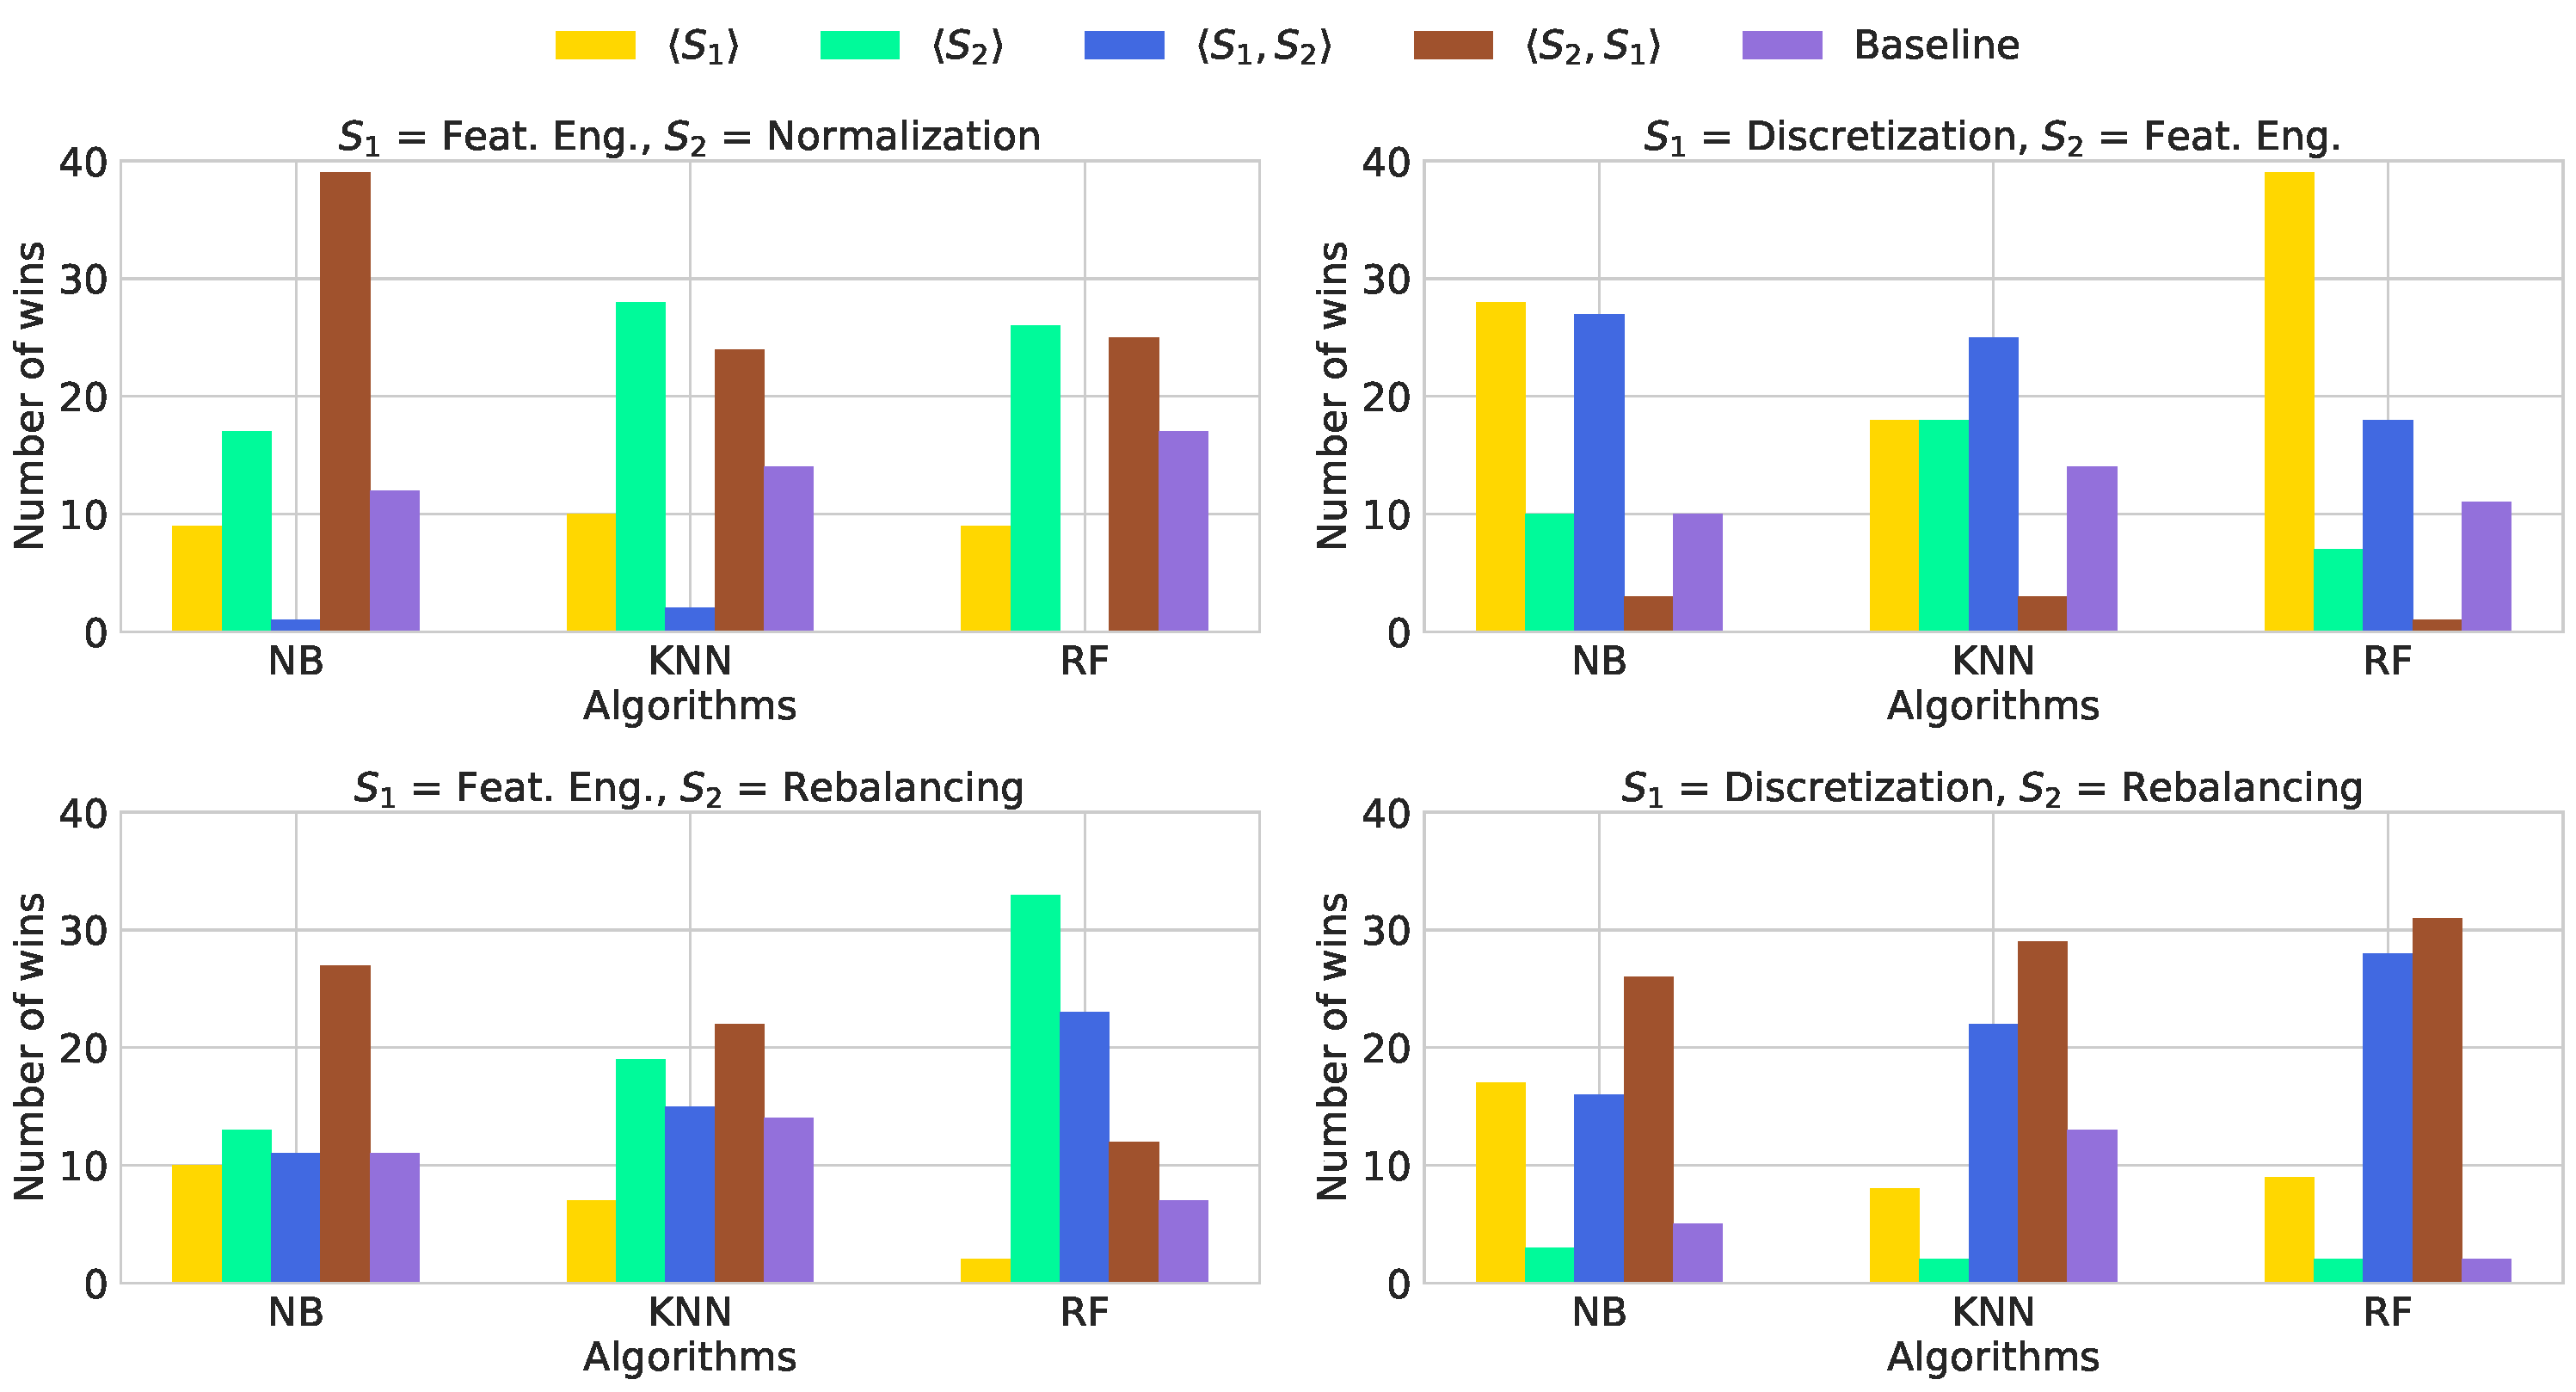
\includegraphics[width=1.0\textwidth]{chapters/data-centric/supervised/img/experiments_results.pdf}
	\caption{Number of datasets for which a given pipeline prototype is declared the winner.}
	\label{effective-fig:learned-rules-results}
\end{figure*}

Applying \Cref{effective-alg:learned-rules}, we obtain a promising order for each pair of transformations considered (i.e., $\{F,N\}$, $\{F,D\}$, $\{F,R\}$, $\{R,D\}$).
Since SMBO is a randomized algorithm, we experimented it with (i) running it several times splitting the budget, and (ii) running it only once with the entire budget.
For the experiments considered, no significant differences where observed, therefore we opted for running it once with the entire budget (i.e., 200 seconds per run), which allows for more configurations to be visited in a single run. Aggregating all the results, \Cref{effective-fig:learned-rules-results} shows the number of datasets, for which a given prototype (\Cref{effective-tbl:validation-rules}, column \textit{winner prototype} for the list of labels) is selected as the winner.
For instance, for the pair $\{F,N\}$ (i.e., Feature Engineering, Normalization), the prototype winning in more datasets for \textit{KNN} and \textit{NB} is $\langle N, F \rangle$.
This means that in general, better results are obtained if Normalization is applied before Feature Engineering.

Next, only $N$ appears as first for \textit{RF} and second best for \textit{KNN} and \textit{NB}, which means that for many datasets, considering different algorithms, it results better to apply only Normalization without combining it with Feature Engineering.
The third position is for $\langle \varnothing, \varnothing \rangle$, which means that for some datasets it is better not to apply any of the steps (in any combination).
The remaining prototypes winning in some datasets are $F$ (only Feature Engineering), and $\langle F, N \rangle$ (Feature Engineering preceding Normalization).
Finally, for three datasets, that are omitted from the figure, there were no winning pipelines (i.e., pipelines resulted in a draw).

Since our goal is to find the best order for a pair of pre-processing steps, we focus on the performances of the pipelines where both of the steps are instantiated (i.e., $\langle S_1, S_2 \rangle$ versus $\langle S_2, S_1 \rangle$).
To do this, we check whether the difference between the number of datasets where they each appear to win is statistically significant by running a binomial test assuming a theoretical probability of $0.5$.
The results are shown in \Cref{effective-tbl:significance-test}.
In summary, the results from \Cref{effective-tbl:significance-test} indicate that, with 95\% confidence we can assume that for the pair $\{F, N\}$, $\langle N, F \rangle$ performs better than $\langle F, N \rangle$, hence Normalization should precede Feature Engineering.
On the other hand, for $\{D, F\}$, $\langle D, F \rangle$ performs better than $\langle F, D \rangle$, hence Discretization should precede Feature Engineering.
Finally, for the remaining transformations, $\{F, R\}$ and $\{R, D\}$, a precedence order can not be pre-assumed since the results obtained are not significant.
Using these results, we create the \textit{Promising precedence} adjacency matrix shown in \Cref{effective-tbl:rules}c, where as one can observe, precedence edges are introduced for $\{N, F\}$ and $\{D, F\}$, but no edges exist neither for $\{F, R\}$, nor for $\{R, D\}$.




\begin{table}[t]
	\centering
	\footnotesize
	\begin{threeparttable}
		\caption{
			Binomial test for determining the order between pairs of transformations. 
		}
		\label{effective-tbl:significance-test}
		\begin{tabular}{@{}cccccc@{}}
			\toprule
			%$S_1$ & $S_2$ & $S_1 \rightarrow S_2$ & $S_2 \rightarrow S_1$ & alpha & \begin{tabular}[c]{@{}c@{}}p-value\\ $H_0:\pi = \pi_0=0.8$\end{tabular} \\ \midrule
			$S_1$ & $S_2$ & $\langle S_1, S_2 \rangle$ & $\langle S_2, S_1 \rangle$ & alpha & p-value\\ \midrule
			$F$ & $N$ & 3 & 88 & 0.05 &  \textbf{0} \\
			$D$ & $F$ & 70 & 7 & 0.05 &  \textbf{0}  \\
			$F$ & $R$ & 49 & 61 & 0.05 & 8.53e-01 \\
			$D$ & $R$ & 66 & 86 & 0.05 & 9.38e-01 \\ \bottomrule
		\end{tabular}
		\begin{tablenotes}
		\centering
		\scriptsize
		\item$N$ - Normalization; $D$ - Discretization; $R$ - Rebalancing; $F$ - Feature Engineering. 
		\end{tablenotes}
	\end{threeparttable}
\end{table}
% \color{black}


\subsubsection{Cross-validation with Chi-square Test}
\label{sec:learned-rules-validation}
After running \Cref{effective-alg:learned-rules} to empirically find a winner between two pairs of transformations, we may obtain a different distribution of the number of wins for the pairs, depending on the datasets considered.
To show that the results obtained with the initial set of datasets are generalizable, we propose to perform an additional cross-validated experiment, where the set of datasets considered can be randomly split into many folds.
Then, for each fold, the results can be compared to the rest, with the aim of checking whether the distributions are similar.
This check can be done via a significance test (e.g., chi-square).
To this end, if the distributions between the folds are similar, it means that the obtained results are independent of the datasets considered, since no matter the combination of the datasets, the results are the same and thus generalizable.

\paragraph{Use case} To show that the results do not depend on the datasests selected, we re-run the experiments (i.e., 10-times each), but this time splitting the datasets into 4-folds.
The goal is to check if the results of the precedence orders from the different folds (i.e., for each experiment considering a randomly different set of datasets) are similar between them (i.e., follow the same distributions).
To confirm this hypothesis, we perform a chi-square test between the results (precedence orders) obtained in a single fold in comparison to the three remaining folds, hence comparing $25$\% of the datasets to the rest.
In particular, to confirm the hypothesis, we need to find results that accept the null hypothesis of the chi-square test which states that ``there is no significant difference between the distributions''.
To do that, sticking to the $95$\% confidence interval, we need to look for p-values greater than $0.05$.
That is, the higher the p-values, the more we accept the null hypothesis, and the more similar the distributions.
Looking at the p-values we found out that they were all much higher than $0.05$.
Specifically, the scores of the chi-square tests of the folds (one fold compared to the rest) are averaged and, after having repeated this procedure 10 times, instead of using a table we depict the 10 averaged p-values using box-plots in \Cref{effective-fig:10-times-4-cv}.
We conclude that, for both of the rules (i.e.,  $\langle F, N \rangle$ and $\langle F, D \rangle$), the significance test indicates a compliance between the new results (\Cref{effective-fig:10-times-4-cv}) and those illustrated above (\Cref{effective-tbl:significance-test}).

\begin{figure*}[!t]
	\centering
	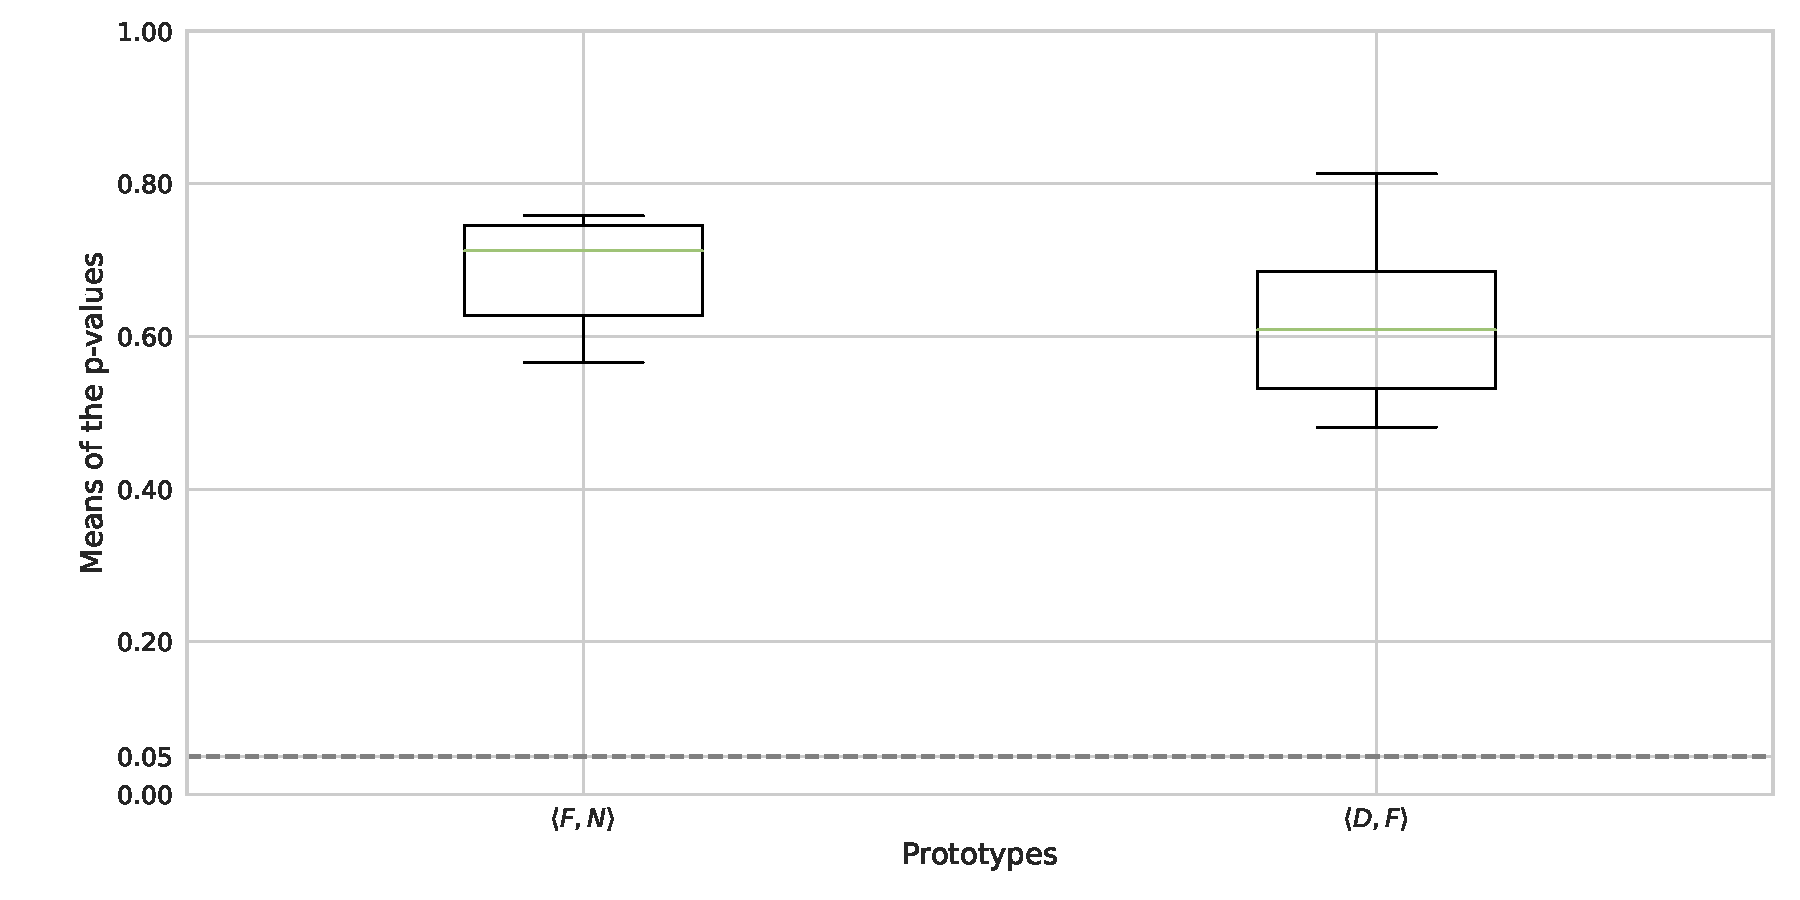
\includegraphics[width=0.9\textwidth]{chapters/data-centric/supervised/img/10_times_4_folds_cv.pdf}
	\caption{The distribution of the p-values obtained after repeating the chi-square test for 10 times, for the 10 times 4-fold cross-validation.}
	\label{effective-fig:10-times-4-cv}
\end{figure*}

\begin{table}[!t]
	\caption{
		Union of rules from \Cref{effective-tbl:rules}.
	}
	\renewcommand{\arraystretch}{0.3}
	\footnotesize
	\centering
	\label{effective-tbl:rules-union}
	\begin{threeparttable}
		\begin{tabular}{p{1cm}p{1cm}p{1cm}p{1cm}p{1cm}p{1cm}p{1cm}}
			\toprule
			& $\boldsymbol{E}$ & $\boldsymbol{N}$ & $\boldsymbol{D}$ & $\boldsymbol{I}$ & $\boldsymbol{R}$ & $\boldsymbol{F}$
			\\	\cmidrule[.1em]{1-7}
			$\boldsymbol{E}$ & \cellcolor{gray!25} & \texttt{1} & \texttt{1} & \texttt{0} & \texttt{1} & \texttt{1} \\	\cmidrule[.1em]{1-7}
			$\boldsymbol{N}$ & \texttt{0} & \cellcolor{gray!25}  & \texttt{X} & \texttt{0} & \texttt{1} & \texttt{1} \\	\cmidrule[.1em]{1-7}
			$\boldsymbol{D}$ & \texttt{0} & \texttt{X} & \cellcolor{gray!25} & \texttt{0} & \texttt{0} & \texttt{1} \\	\cmidrule[.1em]{1-7}
			$\boldsymbol{I}$ & \texttt{1} & \texttt{1} & \texttt{1} & \cellcolor{gray!25}  & \texttt{1} & \texttt{1} \\	\cmidrule[.1em]{1-7}
			$\boldsymbol{R}$ & \texttt{0} & \texttt{0} & \texttt{0} & \texttt{0} & \cellcolor{gray!25}  & \texttt{0} \\	\cmidrule[.1em]{1-7}
			$\boldsymbol{F}$ & \texttt{0} & \texttt{0} & \texttt{0} & \texttt{0} & \texttt{0} & \cellcolor{gray!25} \\	\cmidrule[.1em]{1-7}
		\end{tabular}
		\begin{tablenotes}
			\scriptsize
			\item$\boldsymbol{E}$ - Encoding; $\boldsymbol{N}$ - Normalization; $\boldsymbol{D}$ - Discretization; $\boldsymbol{I}$ - Imputation; $\boldsymbol{R}$ - Rebalancing; $\boldsymbol{F}$ - Feature Engineering. \item \texttt{1} - a precedence edge exists between the row and the column, \texttt{0} - a precedence edge does not exist between the row and the column, \texttt{X} - the combination is meaningless.
		\end{tablenotes}
	\end{threeparttable}
\end{table}

\subsection{Effective Prototypes Composition}
\label{effective-ssec:composition}

In this, we foresee the composition of the previously defined rules (i.e., for the pairs of pre-processing steps), to generate the final set of rules that would allow to compose longer chains---consisting of more than two steps.
This is when we also resolve the inconsistencies and define precedences for the pairs of steps that may not have any precedence defined already---in that case, we basically take into account all the permutations.
This allows to finally generate the possible effective  prototypes.

\paragraph{Use case}
To generate the final prototypes, in this phase, we combine all the matrices generated by the previous steps.
That is, we take the union of the edges (represented by \texttt{1}'s) from the matrices in \Cref{effective-tbl:rules} (a,b,c), and create a new final adjacency matrix, shown in \Cref{effective-tbl:rules-union}.
This is the matrix that will allow us to generate the final effective prototypes.

Observing the table, one can realize that for pairs $\{F,R\}$ and $\{R,D\}$, no precedence edges exist.
This means that these pairs are somewhat equally relevant from either direction (any order), and thus when generating the final prototypes, both options should appear.

For a better reading, in Figure~3.6, we visualize \Cref{effective-tbl:rules-union} in form of a graph, where nodes represent the pre-processing steps and the directed edges represent a precedence order between them.
Out of the graph, we generate the final prototypes by taking all the maximum length variations (ordered arrangements without repetition) of the nodes, respecting the precedence rules (i.e., not contradicting the direction of existing edges).
The result is the set of five prototypes shown in Table 3.7. This set consisting of \textit{compatible}, \textit{meaningful} and \textit{promising} pairs of transformations is the set of recommended \textit{effective pipeline prototypes}.


\begin{figure}
	\begin{floatrow}
	\ffigbox{
		\includegraphics[clip, trim=2.5cm 23cm 10.5cm 2cm,width=0.5\textwidth]{chapters/data-centric/supervised/img/graph.pdf}
	}{
		  \caption{Precedence graph generated from \Cref{effective-tbl:rules-union}.}
	}
	\capbtabbox{
	\begin{tabular}{@{}ll}
				\toprule
				ID& Pipeline prototype                                             \\ \toprule
				1&{\color[HTML]{000000} $\langle I, E, N, R, F  \rangle$} \\
				2&{\color[HTML]{000000} $\langle I, E, N, F, R \rangle$} \\
				3&{\color[HTML]{000000} $\langle I, E, R, D, F \rangle$} \\
				4&{\color[HTML]{000000} $\langle I, E, D, R, F \rangle$} \\
				5&{\color[HTML]{000000} $\langle I, E, D , F, R \rangle$} \\
				\bottomrule
			\end{tabular}
	}{
		  \caption{Effective prototypes generated from Figure~3.6.
		}
	}
	\end{floatrow}
\end{figure}

\subsection{Meta-learning of Instantiation Rules}
\label{effective-ssec:meta-learning}

Once the pipeline prototypes are constructed (i.e., the order between the steps is defined), what follows is their instantiation with the actual transformations.
For that, one can rely completely on SMBO, and let the optimization choose the right transformation for each step.
However, as many optimization techniques, SMBO suffers from the cold-start problem where, in the beginning, it does not have enough information to come up with promising configurations, and a wrong choice may affect the whole process.

\subsubsection{Exploratory Analysis}
Given the availability of the experimental SMBO executions (executed in an exhaustive manner, considering all the prototypes), one can perform an exploratory analysis with the aim of removing useless prototypes, executable pipelines or sngle transformations.
Hence, further tweaking the search space.
In particular, one might analyze whether:

\begin{itemize}
    \item there exist some combination of steps (\Cref{effective-tbl:pipeline-enumeration}), that are generally useless (i.e., in terms of their impact on the final performance), and thus can be discarded a priori to reduce the search space;
    \item there are some executable pipelines that are consistently chosen more often than others by the optimization, meaning that they are more useful than others;
    \item within the executable pipelines, some transformations are chosen more often than others, meaning that they provide a more positive impact.
    \end{itemize}

\paragraph{Use case}
We performed the above-mentioned analysis, but this did not lead to any conclusive or significant results.
In particular, as shown in \Cref{effective-fig:prototypes-impact}, we could not find any useless prototypes---not positively impacting the final accuracy, that could be discarded a priori from the potential list of prototypes.
Actually, as we will show in \Cref{effective-sec:eval-universal-pipeline}, all of them lead to the best in one case or another, which does not mean the epsilon improvement some provide is worth the search cost you incur in considering them (but this more in-depth analysis is done later).
Next, as shown in \Cref{effective-fig:pipeline-frequency}, there were no physical pipelines shown to be more useful---hence more often selected, than others.
Even if $\langle N , R \rangle$ is clearly above, it barely reaches 30\% in KNN.
Finally, observing \Cref{effective-fig:transformation-frequency}, it is clear that some kinds of transformations are chosen more often, but looking closely (i.e., the shaded bars), it is not clear which operator brings more benefit.
For instance, Normalization is present in 90\% of the pipelines, but it is not easy to distinguish which kind of Normalization (i.e., actual operator) is more beneficial.
For this, we need more complex rules or guidelines that may help in finding the right operator to use.


\begin{figure*}[!t]
	\centering
	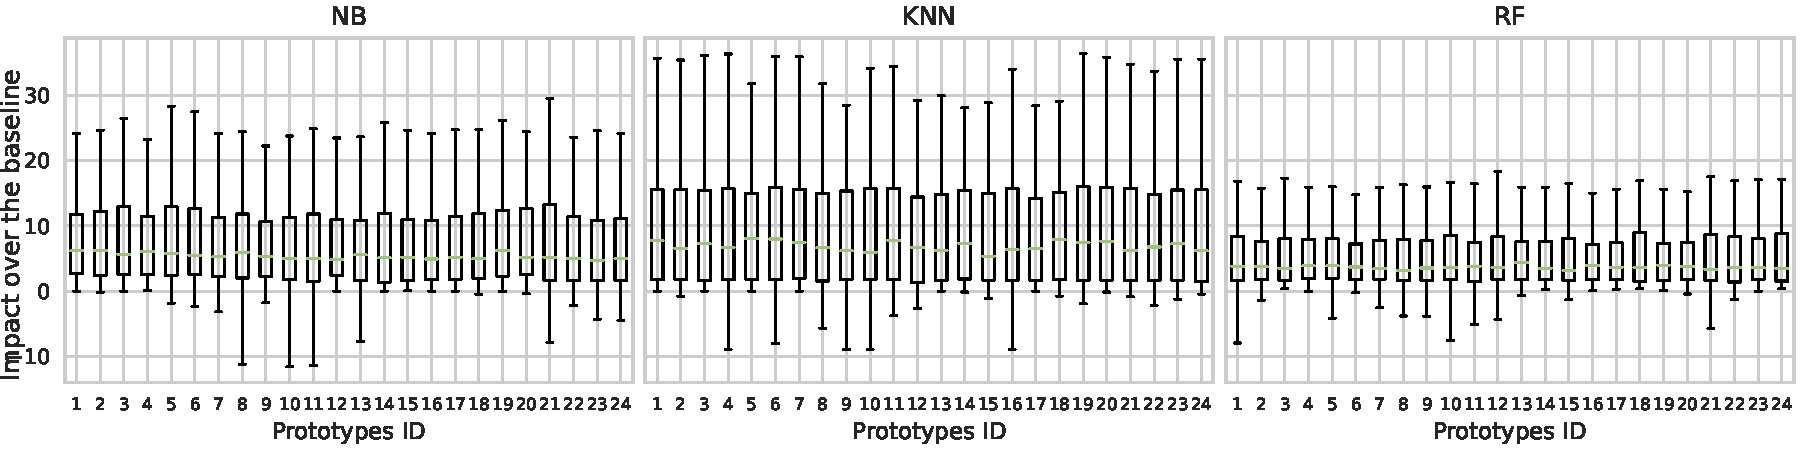
\includegraphics[width=1.0\textwidth]{chapters/data-centric/supervised/img/prototypes_impact.pdf}
	\caption{The impact of the different pipeline prototypes over the baseline (i.e., when no transformation is applied).}
	\label{effective-fig:prototypes-impact}
\end{figure*}

\begin{figure*}[!h]
	\centering
	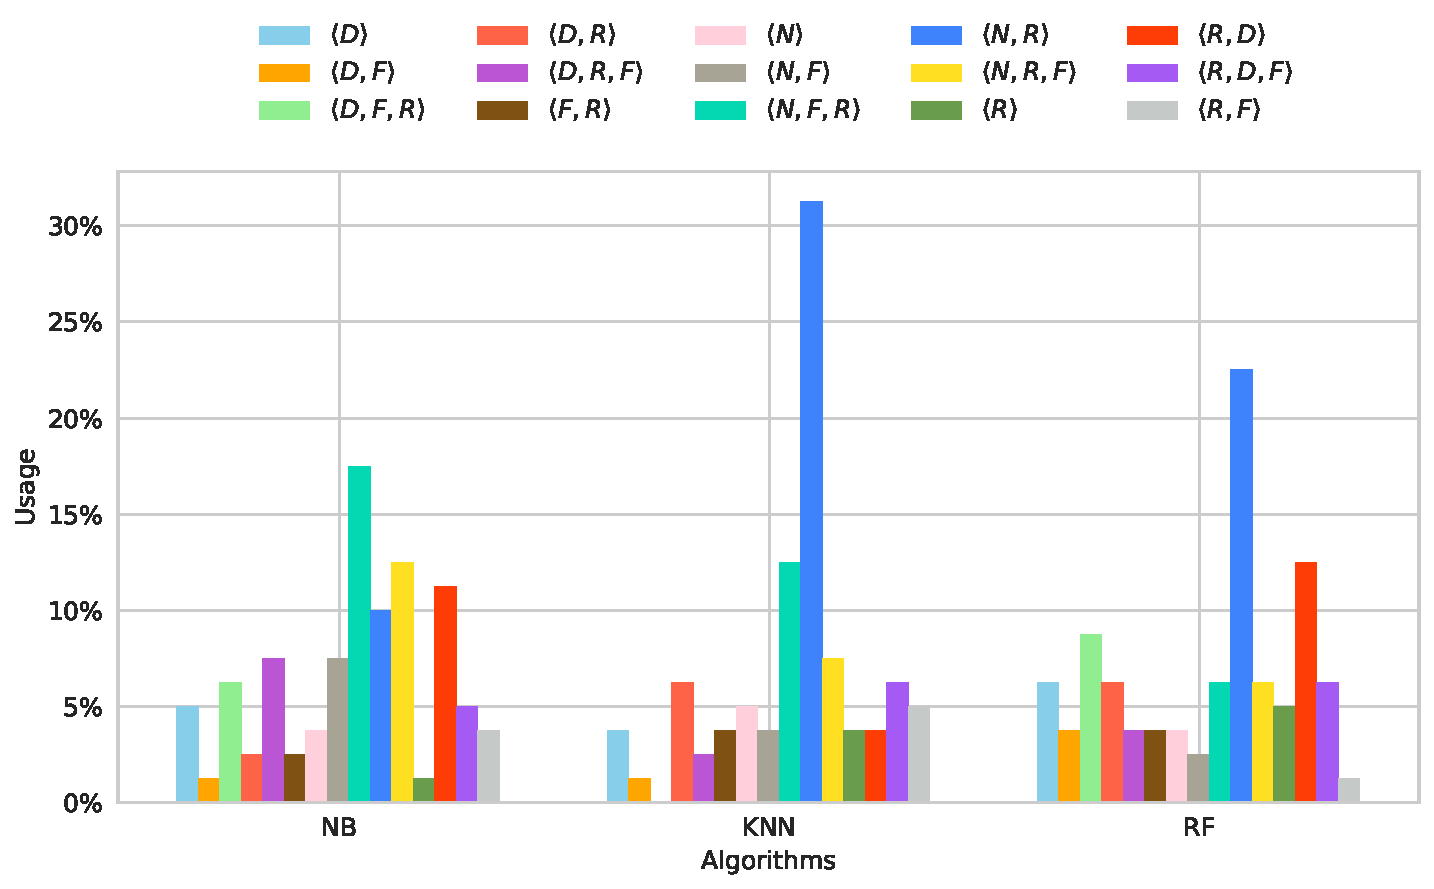
\includegraphics[width=1.0\textwidth]{chapters/data-centric/supervised/img/pp_pipeline_study2.pdf}
	\caption{Percentage of use of the different physical pipelines.}
	\label{effective-fig:pipeline-frequency}
\end{figure*}

\begin{figure*}[!h]
	\centering
	\includegraphics[width=0.7\textwidth]{chapters/data-centric/supervised/img/pp_pipeline_study_grouped.pdf}
	\caption{Percentage of use of a transformation in a physical pipeline.}
	\label{effective-fig:transformation-frequency}
\end{figure*}

\subsubsection{Meta-learning}
To mitigate the cold-start problem, we propose to perform meta-learning, where we intend to use the knowledge extracted from historical data in order to devise rules that may help the optimization in its initial settings.
Meta-learning is the process of ``learning on top of learning'', or learning a model using historical data from ML experiments.
Traditionally, it has been used for predicting the performance (e.g., accuracy) of an algorithm on a given dataset.
That is, given some historical runs of the performance of classification algorithms over various datasets (i.e., meta-dataset: consisting of datasets characteristics as meta-features and the performance of the ML algorithm as the desired outcome in a regression task), one can learn a model (i.e., meta-model), that is able to predict the performance of a given ML algorithm on a new dataset \cite{Brazdil04Book}.
Lately, this technique has been extended in order to predict the impact of pre-processing steps over the performance of ML algorithms and thus rank them based on the impact \cite{Bilalli17AMCS, presistant18CSI, presistant19DKE}.
The same idea can be applied to learning the best trnasformation for a given step.
That is, through meta-learning one can learn the intrinsic relationship between dataset characteristics and the transformation performance, and thus come up with rules that are not obvious and are effective at the time of pipeline instantiation.
The main idea is to build a model, that is able to predict the transformation for a certain pre-processing step, given the meta-features extracted from the dataset considered for the optimization.
This translates to answering the following question: ``given that we know the dataset characteristics and having selected a certain pre-processing step (e.g., Imputation), what is the optimal transformation we need to obtain the highest improvement w.r.t. loss (i.e., when the ML algorithm is applied over the transformed dataset)?''.
In particular, the model can generate a set of complementary rules that help in the optimization, providing a good starting instantiation for some of the steps in the prototype.

To train the model we need a meta-dataset that can be  (i) generated through optimization algorithms (e.g., SMBO executions), (ii) generated manually through simple evaluations of classification algorithms over transformed datasets, or (iii) assumed already given (e.g., OpenML).
Given a meta-dataset, we propose to learn to predict the best instantiation (transformation) for a given pre-processing step, including skipping the step (class \texttt{None}).

\paragraph{Use case}
Our training dataset for the meta-learning (i.e., meta-dataset) is built through SMBO runs on the OpenML datasets (\Cref{effective-ssec:rules-learned}).
We first extract the dataset characteristics (i.e., meta-features; e.g., number of features, number of instances, number of missing values).
Then, by applying SMBO optimization on classification algorithms and pre-processing prototypes, for each dataset, we retrieve the loss (in our case, accuracy) of the ML algorithms over the optimized pipelines.
This gives us the optimized executable pipelines and their impact on the accuracy of the learning algorithms for each dataset at hand.
Given such information, our aim is to now save time and improve the instantiation of the transformations for each step considered in the prototype.

We trained several different conditional inference trees (i.e., a particular implementation of decision trees \cite{ctree}) because they produce models that can be easily read and interpreted.
Specifically, the independence of each meta-feature with the class (transformation of a specific step) is tested through a statistical test.
The split is made on the variable with the lowest p-value.
We report the p-value too so that it can be seen how strong the association is (i.e., why that variable was chosen).
We stick with the p-value threshold of $0.05$, and devise a rule from any branch of the tree that is within the threshold.
In the following, we describe the rules obtained within the selected significance threshold.


\begin{figure}[!h]
	\centering
	\includegraphics[clip, trim=1.0cm 0.4cm 1cm 1cm,width=1\textwidth]{chapters/data-centric/supervised/img/tree-FE.pdf}
	\caption{Conditional Inference Tree built for the \textit{Features Engineering} transformation.}
	\label{effective-fig:features-meta-learning:feature-engineering}
\end{figure}

\textbf{Rules for Feature Engineering}. The available transformations in scikit-learn for Feature Engineering are: Principal Component Analysis (\texttt{PCA}), \texttt{Feature Selection} (Select K Best), \texttt{Both} (PCA + Select K Best), and \texttt{None}.
The tree generated for the Feature Engineering transformation is shown in \Cref{effective-fig:features-meta-learning:feature-engineering}.
The leaves show the selected transformation frequency.
For the sake of simplicity, we do not consider the union of PCA and Select K Best as a transformation per se, instead we distribute that contribution to the two operators that compose it.
Observe that there is a strong correlation between the Feature Engineering transformation and the entropy of the class.
Indeed, such a meta-feature achieved a p-value smaller than $0.001$.
We can clearly read that if the Class Entropy is low, then \texttt{Feature Selection} is way more chosen than the other options (see Node 2).
Recall that entropy is a measure of how much disorder there is in its domain.
The less is that value, the easier is the classification problem.
As a consequence, it is reasonable to think that the easier the classification problem is, the more likely is the fact that the class can be described by a low number of features.
Hence, the \texttt{Feature Selection} technique can be successfully applied.
Conversely, Node 5 shows that, when the Class Entropy is high, it is better to not apply any Feature Engineering operator.
As a matter of fact, a high value of Class Entropy involves a high number of classes and/or few instances per class, hence a really difficult problem.
In such cases, reducing the dimensionality of the dataset does not lead to any improvement.
Finally, when the Class Entropy is in between, there is no clear winner, and thus other non-obvious factors may affect the choice of the operator.

\begin{figure}[!h]
	\centering
	\includegraphics[clip, trim=5.8cm 0.4cm 5.05cm 3.5cm,width=0.65\textwidth]{chapters/data-centric/supervised/img/tree-RE.pdf}
	\caption{Conditional Inference Tree built for the \textit{Rebalancing} transformation.}
	\label{effective-fig:features-meta-learning:rebalancing}
\end{figure}

\textbf{Rules for Rebalancing}. As for Rebalancing, the transformations considered from the imblearn\footnote{\url{https://pypi.org/project/imbalanced-learn}} library are: \texttt{Near Miss}, \texttt{SMOTE}, and \texttt{None}.
The first is an undersampling algorithm which randomly eliminates the samples from the larger class; the second is an oversampling technique that creates samples of the minority class, as a linear combination of them.
As shown in \Cref{effective-fig:features-meta-learning:rebalancing}, the meta-feature Majority Class Percentage has a p-value of $0.014$.
This can be read as, in case of an unbalanced class problem (i.e., Node 3: Majority Class Percentage greater than 56), an oversampling of the minority class(es) is preferred to a downsampling of the majority one(s).
However, when the Majority Class Percentage is smaller than 56\%, the situation is not that clear, and there is no technique that is applied significantly more often than the rest; they are close to each other.
Therefore, it is difficult to understand which problems (which dataset characteristics do they have) belong to Node 2.
In summary, when the majority class has no more than 56\% , it implies that it is an unbalanced class, and as mentioned above, SMBO tends to choose the same transformation.
However, when the majority class has less than 56\%, it may imply that: (i) there are just two classes and the problem counts as a balanced problem, so no transformation needs to be applied, or (ii) it is a multi-class problem, and thus there is no clear winner in terms of transformation.

\subsection{Data Pipeline Instantiation}
\label{effective-ssec:prototype-insta}

The prototypes from the top flow and the meta-lerning rules from the bottom flow (if the optimization framework permits) are finally fed to the final phase which deals with the instantiation and optimization of the prototypes. In this, we run SMBO until an optimized pipeline is found.

\paragraph{Use case}
 In our final execution, we run SMBO to find a suitable instantiation for the suggested prototypes. The simple but not obvious meta-learning rules, even though not included in our final execution, because of the implementation considered (i.e., HyperOpt), can potentially be used to ease the cold-start problem.

\section{Empirical Evaluation}
\label{effective-sec:evaluation}


The aim of our experimental study is three-fold:
\begin{enumerate}
    \item Check whether there exists a universal prototype that works best for any classification problem considered  (i.e., dataset and ML algorithm) (\Cref{effective-sec:eval-universal-pipeline}).
    \item Assess and compare the performance of optimizing the effective prototypes constructed using our method against the set of exhaustively generated prototypes (\Cref{effective-sec:eval-our-vs-rest}).
    \item Assess and compare the impact of dedicating a portion of the optimization time to the effective prototypes against using the whole optimization time for the hyperparameters of the ML algorithm (\Cref{effective-sec:eval-dpso-vs-cash}).
\end{enumerate}

The experiments were performed on an Intel Core i7 machine with 12 cores, running at 3.20 GHz with 64 GB of main memory.
We leveraged the SMBO optimization algorithm available in the Python library HyperOpt \cite{bergstra2015hyperopt}.
The datasets used in the experiments are the ones from the OpenML CC-18 repository \cite{OpenML2013}.
Finally, the classification algorithms considered are \textit{NB}, \textit{KNN}, and \textit{RF} from the Python library Scikit-learn \cite{scikit-learn}.
All the experiments for a single algorithm took approximately two weeks.


\paragraph{AutoPrep}
With the recent shift towards data-centric approaches, rather than algorithmic, data pre-processing is receiving a lot of attention.
Yet, its impact on the final analysis is not widely recognized, primarily due to the lack of publicly available experiments that quantify it.
To bridge this gap, along with this work, we contribute to publishing a companion reproducibility paper \cite{Giovanelli2022IS} for the experiments and results reported in the following.
AutoPrep introduces a set of reproducible experiments on the impact of data pre-processing by providing a detailed reproducibility protocol together with a software tool and a set of extensible datasets, which allow for all the experiments and results of this chapter reproduced.
Our experiments have been performed among different machines with different resources.
We achieved to deploy \textit{strongly reproducible experiments}, when based on a collection of intermediate results, and \textit{weakly reproducible experiments} when reproducing our end-to-end optimization from scratch.
The reproducibility protocol is created in Docker and tested in Windows and Linux.
The source code and the datasets for reproducing the experiments can be found on GitHub\footnote{
\url{https://github.com/josephgiovanelli/autoprep}}.

\begin{definition}[Strongly reproducible experiment  \cite{reproducible}]
    \label{def:strong}
    Given a set of previously reported experimental results and conclusions, a computational experiment is strongly reproducible if it allows to confirm both previously reported results and conclusions exactly.
\end{definition}

\begin{definition}[Weakly reproducible experiment  \cite{reproducible}]
    \label{def:weak}
    Given a set of previously reported experimental results and conclusions, a computational experiment is weakly reproducible if the Spearman rank correlation between the original and reproduced results is equal to 1, and their Pearson correlation value is high enough to allow the confirmation of all previously reported conclusions, even if the reproduced results do not reproduce all results exactly. Thus, weak reproducibility is a performance-rank-preserving notion.
\end{definition}

\subsection{Universal Pipeline Prototype}
\label{effective-sec:eval-universal-pipeline}
The goal of this experiment is to demonstrate the difficulty of blindly finding the right prototype (i.e., without considering any meaningful or promising precedence).
In \Cref{effective-tbl:pipeline-enumeration}, we list the exhaustive set of pipeline prototypes generated considering the compatible precedence graph in Table~\ref{effective-tbl:rules}a (i.e., 24 compatible permutations).
In a real scenario, this number would be too high for splitting the time budget in order to optimize them.
Yet, for the sake of this experiment, we exhaustively optimize all the prototypes, for each dataset.
Thus, for each prototype and for each dataset, the SMBO algorithm is configured to assign a 200 seconds time budget to the phase of instantiating and optimizing the prototype, and another 200 seconds to the phase of optimizing the hyperparameters of the ML algorithm.

\begin{table}[t]
\caption[Enumeration of the prototypes that can be generated by compatible precedence]{Exhaustive set of prototypes generated using the compatible precedence graph of Table~\ref{effective-tbl:rules}a. $E$ - Encoding; $N$ - Normalization; $D$ - Discretization; $I$ - Imputation; $R$ - Rebalancing; $F$ - Feature Engineering.
}
\footnotesize
\label{effective-tbl:pipeline-enumeration}
\begin{center}
\begin{tabular}{@{}lllll@{}}
\toprule
ID & Pipeline prototype & ID & Pipeline prototype                                                                   \\ \toprule
1  & {\color[HTML]{000000} $\langle I, E, N, D, F, R \rangle$} & 13 & {\color[HTML]{000000} $\langle I, E, F, N, D, R \rangle$} \\
2  & {\color[HTML]{000000} $\langle I, E, N, D, R, F \rangle$} & 14 & {\color[HTML]{000000} $\langle I, E, F, N, R, D \rangle$} \\
3  & {\color[HTML]{000000} $\langle I, E, N, F, D, R \rangle$} & 15 & {\color[HTML]{000000} $\langle I, E, F, D, N, R \rangle$} \\
4  & {\color[HTML]{000000} $\langle I, E, N, F, R, D \rangle$} & 16 & {\color[HTML]{000000} $\langle I, E, F, D, R, N \rangle$} \\
5  & {\color[HTML]{000000} $\langle I, E, N, R, D, F \rangle$} & 17 & {\color[HTML]{000000} $\langle I, E, F, R, N, D \rangle$} \\
6  & {\color[HTML]{000000} $\langle I, E, N, R, F, D \rangle$} & 18 & {\color[HTML]{000000} $\langle I, E, F, R, D, N \rangle$} \\
7  & {\color[HTML]{000000} $\langle I, E, D, N, F, R \rangle$} & 19 & {\color[HTML]{000000} $\langle I, E, R, N, D, F \rangle$} \\
8  & {\color[HTML]{000000} $\langle I, E, D, N, R, F \rangle$} & 20 & {\color[HTML]{000000} $\langle I, E, R, N, F, D \rangle$} \\
9  & {\color[HTML]{000000} $\langle I, E, D, F, N, R \rangle$} & 21 & {\color[HTML]{000000} $\langle I, E, R, D, N, F \rangle$} \\
10 & {\color[HTML]{000000} $\langle I, E, D, F, R, N \rangle$} & 23 & {\color[HTML]{000000} $\langle I, E, R, D, F, N \rangle$} \\
11 & {\color[HTML]{000000} $\langle I, E, D, R, N, F \rangle$} & 23 & {\color[HTML]{000000} $\langle I, E, R, F, N, D \rangle$} \\
12 & {\color[HTML]{000000} $\langle I, E, D, R, F, N \rangle$} & 24 & {\color[HTML]{000000} $\langle I, E, R, F, D, N \rangle$}
\\ \bottomrule
\end{tabular}
\end{center}
\end{table}

The results obtained are shown in \Cref{effective-fig:eval-universal-pipeline}.
The enumerated prototypes are listed in the abscissa axis and each stacked bar represents the percentage of cases for which that prototype achieved the best performance across different ML algorithms (the contribution of each algorithm is represented with a different color).
In an ideal scenario, for a prototype to be considered \textit{universal}, it should perform best in all or at least most of the cases, which is clearly not happening.
Observe that, even the best-performing prototype is only the best in 19\% of the cases, which is obviously far from being \textit{universal}.
Hence all (or at least several) prototypes need to be evaluated together, in order to obtain better solutions.

\begin{figure}[t]
    \centering
    \includegraphics[width=0.8\textwidth]{chapters/data-centric/supervised/img/evaluation1.pdf}
    \caption{Comparison of the goodness of the exhaustive set of prototypes.}
    \label{effective-fig:eval-universal-pipeline}
\end{figure}

\subsection{Exhaustive Versus Effective Prototypes}
\label{effective-sec:eval-our-vs-rest}
Given that there is no single universal prototype, one can opt for feeding all the possible prototypes (see \Cref{effective-tbl:pipeline-enumeration}) to the optimization algorithm in order to get the best solutions out of them.
As before, we assign a budget of 200 seconds for the optimization of each prototype, hence 80 minutes in total for all the set of 24 \textit{exhaustive prototypes} in order to find the optimal pipeline for every dataset.
On the other hand, we take only the five \textit{effective prototypes} resulting from the application of our method and assign just 40 seconds time budget for the optimization of each one of them, hence 200 seconds in total. With the aim of comparing the two, and thus roughly understanding how close we are to the optimal case, in both cases, we dedicated the same time budget (i.e., 200 seconds) for the phase of optimizing the hyperparameters of the ML algorithm.
In order to evaluate how close the \textit{effective prototypes} are to the \textit{exhaustive ones}, we calculate the \textit{normalized distance} from the result to the optimum---w.r.t. accuracy.

\begin{equation*}
    normalized\;distance = \frac{ACC_{\textup{eff}} - ACC_{\varnothing}}{ACC_{\textup{exh}} - ACC_{\varnothing}}
\end{equation*}

$ACC_{\varnothing}$ is the baseline performance (i.e., accuracy of the algorithm $A$ with default hyperparameters and no data pipeline, hence computed over the original dataset $\altmathcal{D}$), formally $ACC_{\varnothing} = ACC( \langle \varnothing, A  \rangle (\altmathcal{D}_{train}), \altmathcal{D}_{valid})$.
$ACC_{\textup{eff}}$ is the accuracy of the optimized algorithm $A_{{\lambda}^{\star}}$ over the dataset transformed using the optimized instantiation of the effective set of prototypes (i.e., our approach), formally $ACC_{\textup{eff}} = ACC(\langle P^{\star}_{\textup{eff}_{{\lambda}^{\star}}}, A_{\lambda^\star} \rangle (\altmathcal{D}_{train}), \altmathcal{D}_{valid})$.
Finally, $ACC_{\textup{exh}}$ is the accuracy of the optimized algorithm $A_{{\lambda}^{\star}}$ over the dataset transformed using the optimized pipeline instantiation of the exhaustive set of prototypes, formally $ACC_{\textup{exh}} = ACC(\langle P^{\star}_{\textup{exh}_{{\lambda}^{\star}}}, A_{\lambda^\star} \rangle (\altmathcal{D}_{train}), \altmathcal{D}_{valid})$.
The subtraction by $ACC_{\varnothing}$ is done with the aim of weighting the difficulty of a dataset, hence allowing for comparisons in terms of the gain in accuracy.
To this end, the bigger the potential gain (denominator) is, the bigger the obtained gain (numerator) must be, for the latter to be relevant.

The results obtained for every dataset and algorithm are shown as boxplots in \Cref{effective-fig:eval-exhaustive-vs-effective}.
Observe that, most of the cases are very close to the results obtained using the exhaustive set, the median distances being 91.51\%, 93.13\%, 88.97\%, for NB, KNN, and RF, respectively.
In general, in 75\% of the cases the chosen pipelines are above 80\%, and only few outliers are below 60\%.
Curiously, in some cases, we outperform the results over the exhaustive set of pipelines, but this is due to the randomness of the optimization algorithm, which unless it is given an unrealistically high budget of time, is not capable of finding the true optimal solution.
We discarded the option of assigning a larger budget since this was not practical considering the huge search space and the lack of any guarantee of improvement.

To summarize, the experiment shows that with roughly 24 times less time budget, we can obtain results that are as good as 90\% in the median compared to the exhaustive ones.
The raw results (i.e., without the normalized distances) can be found on the aforementioned GitHub page.

\begin{figure}[!t]
    \centering
    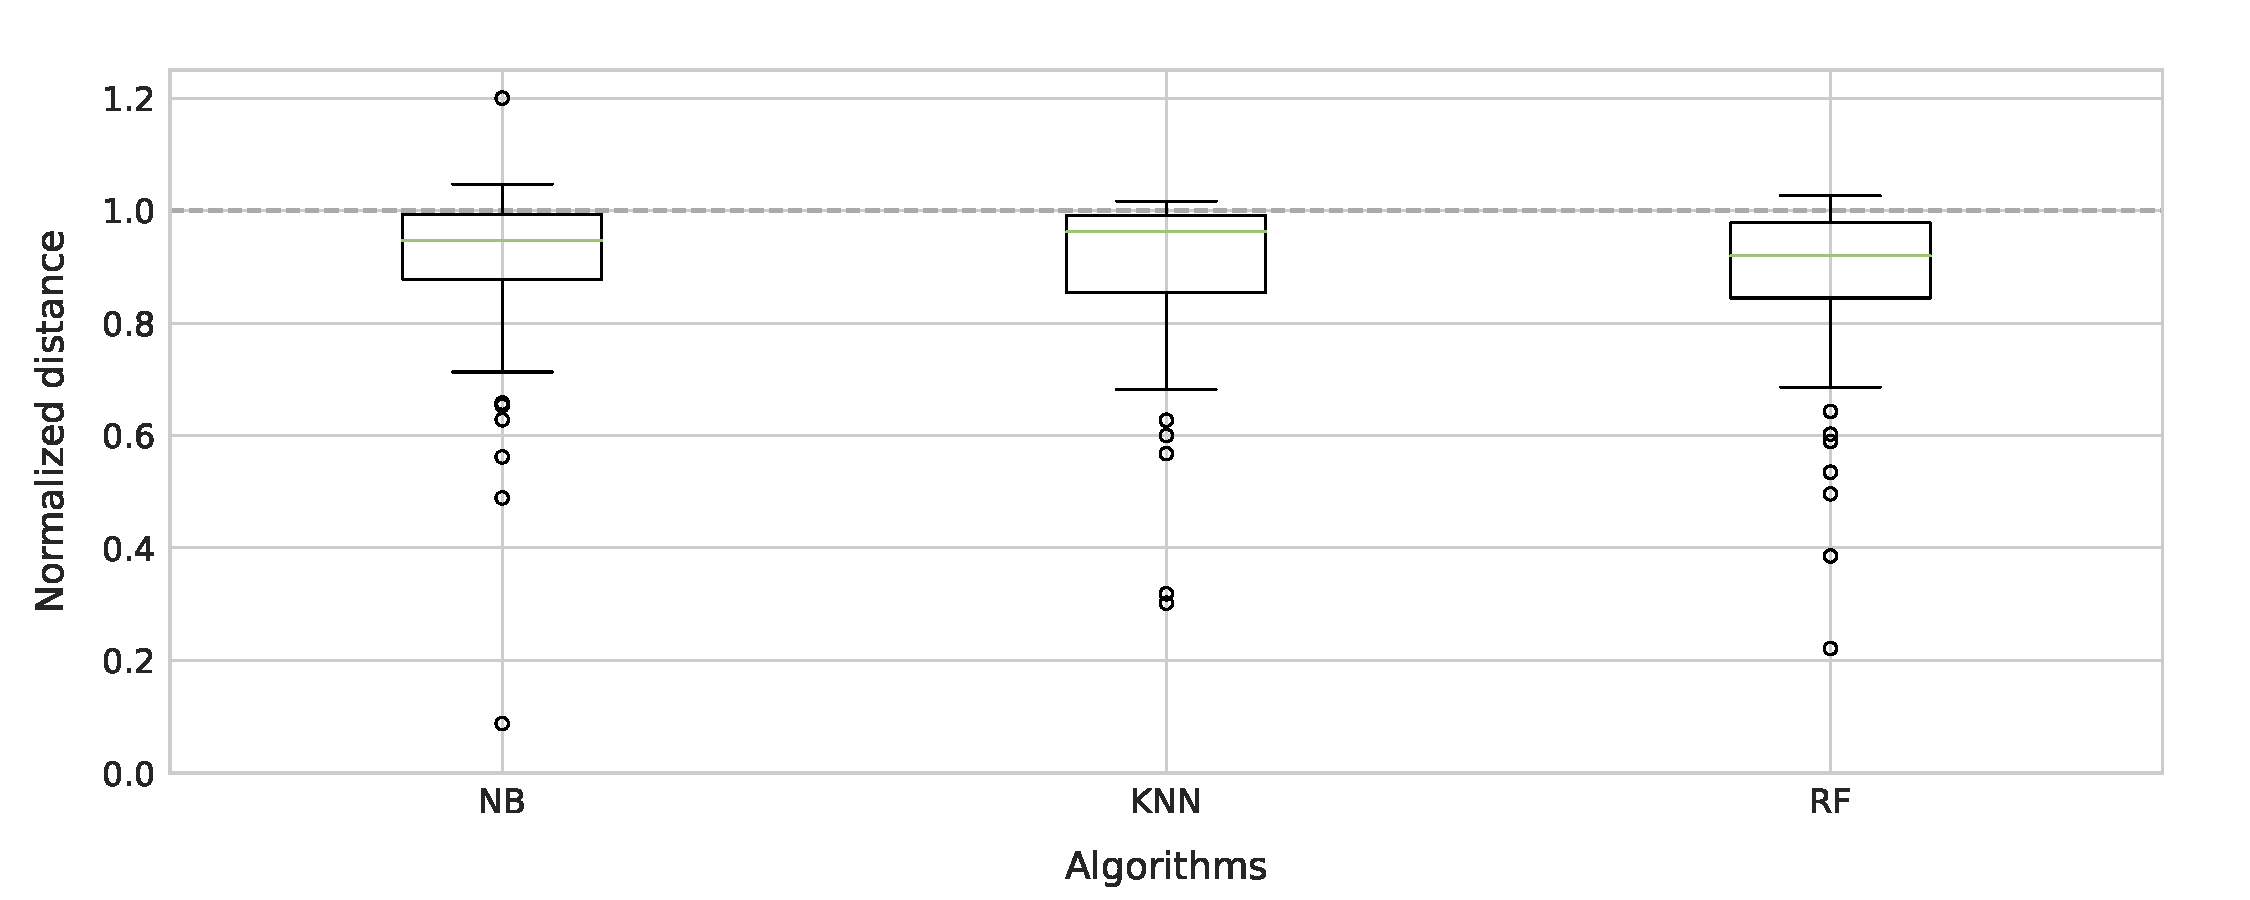
\includegraphics[width=1.0\textwidth]{chapters/data-centric/supervised/img/evaluation2.pdf}
    \caption{Normalized distances between the scores obtained by optimizing our effective prototypes and the ones obtained by optimizing the exhaustive set.}
    \label{effective-fig:eval-exhaustive-vs-effective}
\end{figure}

\subsection{Complementing HPO of ML algorithm with Pre-processing}
\label{effective-sec:eval-dpso-vs-cash}

\begin{figure*}[!t]
	\centering
	\includegraphics[width=1.0\textwidth]{chapters/data-centric/supervised/img/barplot-10.pdf}
	\caption{The impact of dedicating a portion of the optimization budget to pre-processing compared to using the whole optimization budget for the ML algorithm HPO.}
	\label{effective-fig:eval-pre-processing-hyperparameter}
\end{figure*}

We have just shown that our effective prototypes have similar impact as the exhaustive ones.
Now we want to compare the impact of the effective prototypes against optimizing only the hyperparameters of the ML algorithm.
That is, we want to examine whether dedicating a part of the optimization budget to the pre-processing impacts more (positively) the results of the analysis, than using the whole budget for solely the hyperparameter optimization of the ML algorithm\footnote{To enable the application of the ML algorithms on all the datasets, whenever required, we apply the necessary transformation (e.g, imputation or encoding).}---i.e., modelling.

To this end, for the latter we now dedicate the total optimization budget (i.e., 400 seconds), and for the former, inspired by \cite{Quemy20InfSystems}, we split the budget 50-50 between the pre-processing pipeline optimization and the hyperparameter optimization (i.e., 200 seconds for the pre-processing, and 200 seconds for the hyperparameter optimization).
The time for the pre-processing is further split among the five different pipeline prototypes (i.e., 40 seconds each).

To compare the results, we calculate the impact using the formulas below, which correspond to the normalized distance from either pre-processing or hyperparameter optimization to the maximum improvement that can be achieved, regardless of whether pre-processing is applied or not.

\begin{equation*}
    \text{\textit{pp impact}} = \frac{ACC_{\textup{eff}} - ACC_{\varnothing}}{max(ACC_{\textup{eff}}, ACC_{\textup{hpo}}) - ACC_{\varnothing}}
\end{equation*}

\begin{equation*}
    \text{\textit{hp impact}} = \frac{ACC_{\textup{hpo}} - ACC_{\varnothing}}{max(ACC_{\textup{eff}}, ACC_{\textup{hpo}}) - ACC_{\varnothing}}
\end{equation*}

$ACC_{\varnothing}$ is yet again the baseline performance (i.e., accuracy of the algorithm $A$ with default hyperparameters over the original dataset $\altmathcal{D}$).
$ACC_{\textup{eff}}$ is still the accuracy of our approach, i.e., the optimized algorithm $A_{{\lambda}^{\star}}$ with half of the whole budget over the dataset transformed using the optimized instantiation of the effective set of prototypes (with half of the whole budget).
Finally, $ACC_{\textup{hpo}}$ is the accuracy of the optimized algorithm $A_{{\lambda}^{\star}}$ (i.e, using the entire budget) over the original dataset, formally $ACC_{\textup{hpo}} = ACC( \langle A_{{\lambda}^{\star}} \rangle (\altmathcal{D}_{train}), \altmathcal{D}_{valid})$.

To obtain relative values that sum to 1, we normalize the impacts dividing them by their sum.
For instance, for the pre-processing score we calculate the following:
\begin{equation*}
    \text{\textit{normalized pp impact}} = \frac{\text{\textit{pp impact}}}
    {\text{\textit{pp impact}} + \text{\textit{hp impact}}}
\end{equation*}


We perform the same for the hyperparameter impact and plot the results obtained for all the algorithms and datasets in \Cref{effective-fig:eval-pre-processing-hyperparameter}, where each bar represents the results obtained for a single dataset.
The different colors represent the impact values of pre-processing and hyperparameter optimization.

Observing the bar charts one can see that (i) dedicating a portion of the budget to pre-processing, brings benefit to the analysis in most of the cases (i.e., $73\%$ of the cases), and (ii) the impact of hyperparameter optimization, increases with the increase of the number of hyperparameters of the ML algorithm (e.g., hyperparameter optimization impacts more RF than NB).
Overall, we can conclude that pre-processing is a critical step that once effectively applied may have a high positive impact on the final result of the analysis.

\section{Conclusions and Future Works}
\label{effective-sec:conclusions}

In this chapter, we first studied the overall impact of pre-processing steps when chained together inside prototypes and then delved into examining the impact of instantiating steps via various transformations.
As a result, we defined a method that allows to generate effective pre-processing pipelines.
That is, pipelines that consist of, (i) compatible pairs of steps concerning the framework used,  (ii) meaningful pairs of steps in terms of general knowledge (best practices), and (iii) promising pairs of steps that once applied are expected to provide higher overall impact (domain knowledge).
In addition, via the meta-learning phase proposed, we aim to guide the pipeline instantiation in order to facilitate finding better transformations.

An extensive evaluation on 80 datasets with heterogeneous characteristics, from sample size to feature types, and a set of classification algorithms (i.e., Naive Bayes, Random Forest, K-Nearest Neighbours), showed that our devised prototypes give promising results.
More specifically, we were able to observe that:
\begin{itemize}
    \item [--] The overall impact of optimizing pre-processing is not negligible and it may boost the performance of the overall analytics (e.g., accuracy).
    \item [--] There is no universal pre-processing prototype that works best for every dataset and algorithm.
    \item [--] With 24 times less time budget, our proposed prototypes were able to obtain results that were as good as 90\% in the median of the optimal ones found through an exhaustive search.
    \item [--] Dedicating a portion of the time to the pre-processing optimization, instead of dedicating it entirely to hyperparameter optimization may boost the final result of the analysis.
	On average, in 73\% of the cases including pre-processing in the optimization, outperformed the results of only optimizing hyperparameters.
\end{itemize}

The results indicate that pre-processing can boost the performance of the ML algorithm.
Hence, it must be considered as an integral part of the data analytics optimization process.

Finally, previous works have shown the effectiveness of meta-learning for solving the cold start problem \cite{Feurer15AAAI}, hence as immediate future work, we intend to extend an optimization framework (i.e., HyperOpt) with a complementary meta-learning module that can ease the cold-start problem, facilitating the search for optimal instantiations.
\chapter{Supervised Learning}
\label{automl-chap:supervised}

\section{Effective Data Pre-processing}

\subsection{Introduction}

The decision making process has historically been key for the success of any organization or business activity.
Lately, with the abundant presence of data, this process has become data-driven,
where data are continuously analyzed to be transformed into knowledge.
Along the way however, data undergo several (sometimes necessary) processing steps, shown in Figure~\ref{fig:data-analytics-pipeline}. Firstly, data are extracted in a raw format from different sources and then are sifted out such that only a relevant subset is selected. Next, this subset is pre-processed and is fed to a machine learning (ML) algorithm for it to be analyzed. The output of the analysis is then interpreted and the whole process iterates until the results obtained are satisfactory and significant for the decisions to be made. 

Unfortunately, this well known process does not have universal well-defined practices for the different steps, which translates to the data scientist manually configuring and parameterising the operators for each step until an optimal solution is found --- an optimal \textit{data analytics pipeline}. To this end, most of the time is spent on the heavily laborious work of pre-processing (i.e., 50-80\% of the time~\cite{Munson09Pre}), where the generated output is a \textit{pre-processing pipeline}. Next, once the data is transformed into the proper form, different ML algorithms with different hyperparameters are evaluated over the dataset until an acceptable result is obtained --- \textit{ML model}. This whole process requires expertise and is particularly challenging for novice, inexperienced data scientists for whom hand-tuning is no longer an option.

Recent developments in algorithm configuration have raised the efficiency and effectiveness of automatic search, and therefore, for instance, AutoML is now considered a prominent technique for finding optimal models. Some AutoML frameworks~\cite{auto_sklearn,mohr2018ml}, mix-in the pre-processing during the optimization, but they are typically limited to very few transformations or do not consider all the data processing phases (e.g., extraction, selection, loading), thus in a way overlooking it. Inspired from~\cite{Munoz09DOLAP}, we contend that there is need for more generic AutoETL techniques, encompassing all the phases of the ETL  process~\cite{Vaisman14Book}; from its inception via \textit{data extraction}, to the intermediate phase of \textit{data transformation}, up to the final phase, when data reaches its destination, via \textit{data loading}. Assistance is required in every phase~\cite{Bilalli16IOTBD}. Yet, in a data analytics context, as in the case of this work, the critical automation challenge lies more on the \textit{data transformation} phase (see AutoETL and AutoML in Figure~\ref{fig:data-analytics-pipeline}), which is related to the pre-processing of the data.
In the literature, this particular problem has been often referred to as the Data Pipeline Selection and Optimization problem (DPSO)~\cite{Quemy19DOLAP}, where a \textit{pipeline prototype} (sequence of transformations, e.g., missing value imputation followed by normalization) is fed to an optimizer and an optimal instance of the prototype, in the form of a \textit{pipeline} (sequence of operators, e.g., imputation by mean followed by min-max normalization) is found. By considering pre-processing as an integral component of data analytics, and carefully configuring the pre-processing pipelines, it is easy to obtain results that go beyond the ones obtained by only optimizing the learning algorithm. 

\begin{figure*}[t]
    \centering
    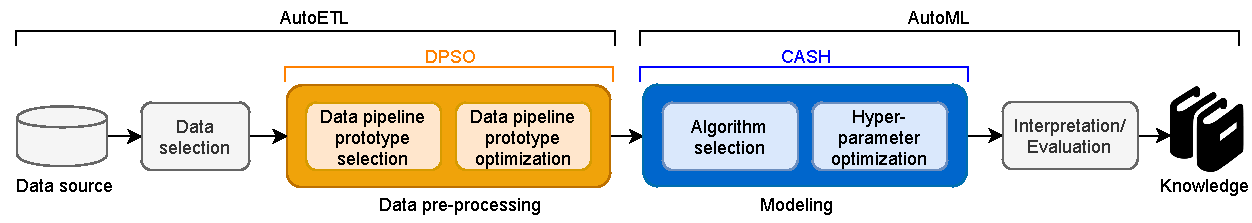
\includegraphics[width=1.0\textwidth]{part-automl/chapter-supervised/img-effective/data-analytics-pipeline.pdf}
    \caption{Data analytics pipeline generation in a knowledge discovery process.}
    \label{fig:data-analytics-pipeline}
\end{figure*}

To briefly illustrate this, we perform an experiment on the well known \texttt{bank-marketing}\footnote{\url{https://archive.ics.uci.edu/ml/datasets/Bank+Marketing}} dataset, using HyperOpt~\cite{HyperOptICML13} as an AutoML approach to optimize the parameters of three different ML algorithms, namely Naive Bayes (NB), K-Nearest Neighbor (KNN), and Random Forest (RF). We provide an initial budget of 50 iterations for optimizing the hyper-parameters of the algorithms, and after the 50th iteration, we fix the algorithm configuration to the best one achieved so far and start optimizing the pre-processing pipeline\footnote{This order is used only for the sake of illustration.}.
In Figure~\ref{fig:pre-processing-impact}, the ratio of the change in terms of predictive accuracy (i.e., ratio of the accuracy obtained after the i-th iteration to the baseline/default accuracy) is plotted against the number of different configurations visited by HyperOpt (i.e., iterations). Observe that after the 11th iteration for NB and KNN, and after the 26th iteration for RF, the lines remain flat. That is, from there on, no improvement is achieved by optimizing the hyper-parameters of the algorithms until the 50th iteration is reached. At this point, a sudden jump is observed and the results start to improve again, going clearly beyond the ones obtained before, thanks to the optimizations performed now over the pre-processing pipeline.
\begin{figure}[t]
    \centering
    \includegraphics[width=0.7\textwidth]{part-automl/chapter-supervised/img-effective/pre-processing-impact.pdf}
    \caption{Evolution of predictive accuracy during the optimization process. The first 50 configurations optimize only the hyper-parameters and after the 50th configuration, the pre-processing pipeline is optimized instead.}
    \label{fig:pre-processing-impact}
\end{figure}
Yet, including the pre-processing in a free form in the optimization, heavily increases the search space, making the problem much harder. This is mitigated by creating a pre-processing pipeline prototype that fixes the order of transformations, leaving the freedom to only instantiate and parametrise them. Therefore, the challenge for data scientists is to find the right pre-processing pipelines, that is, (i) how to order the transformations  (i.e., prototype construction), and (ii) which pre-processing operators to consider in the prototype (i.e., prototype instantiation) such that when optimizing the parameters, better results are obtained.
The aim of this work is to study these two questions in order to propose a method for generating effective pre-processing pipeline prototypes that, once instantiated through some optimization technique (e.g., Bayesian optimization), improve the final result of the analysis.
To keep discussions and experiments simpler, we stick to supervised learning tasks, which encompass algorithms generating a map function based on pairs of input-output exemplars. In particular, this work focuses on classification problems (i.e., binary and multiclass), where the output to be predicted is of Categorical type. Furthermore, this work extends~\cite{Giovanelli2021DOLAP}, among others with, (i) a new meta-learning step to guide the instantiation of transformations where a model is learned to predict the operators for a given transformation (see Section~\ref{ssec:meta-learning}),
(ii) a set of rules extracted through the meta learning process that mitigate the cold start problem (see Example 8), (iii) a new cross validation to confirm the initial results (see Section~\ref{ssec:rules-learned}),
(iv) a new background section for AutoML and AutoETL (see Section~\ref{ssec:background}), and (v) experiments over new datasets (see Section~\ref{ssec:evaluation}). 


\noindent\textbf{Contributions.} The main contributions of this paper can be summarized as follows:
\begin{itemize}
    \item We empirically evaluate the impact of optimizing the exhaustive set of potential pipeline prototypes and find out that at least one different pipeline works best for each dataset and algorithm considered, hence showing that there is no universal pipeline that works best for all of them.
    \item We define a method that given a classification algorithm and a set of pre-processing transformations, is capable of generating the right order between transformations, obtaining effective pre-processing pipeline prototypes, which are then instantiated and further optimized via Bayesian optimization.
    \item We suggest a meta-learning step, where the relationship between pre-processing operators and dataset characteristics is learned in order to create rules that help with the initial instantiation of the pipeline prototypes.
    \begin{itemize}
         \item We exemplify our meta-learning study generating simple but not obvious and effective rules for two kinds of transformations, namely, Feature Engineering and Rebalancing.
    \end{itemize}
    \item We perform a comprehensive evaluation by comparing the performance of optimizing the pipelines generated following our method, and find out that: 
    \begin{enumerate}
        \item with 24 times less time budget, our proposed pipelines obtain results whose median is above 90\% of the ones generated via exhaustive search.
        \item on average, in 73\% of the cases, splitting evenly the time budget between pre-processing and hyper-parametrisation outperforms the results of only optimizing the hyper-parameters of the ML algorithm.
    \end{enumerate}
\end{itemize}

The remaining of this paper is organized as follows. Section~\ref{ssec:background} provides a brief background on AutoETL and AutoML.  Section~\ref{ssec:methodology} presents our method of generating effective pipelines. 
Section~\ref{ssec:evaluation} provides an extensive evaluation of the pipelines created using our proposed method. Section~\ref{ssec:relatedwork} discusses the related work. Finally, Section~\ref{ssec:conclusions} provides the conclusions and future work.

\subsection{Background: AutoETL and AutoML}
\label{ssec:background}


The abundance of data has led to data analytics being prevalent in many disciplines and domains, but since the number of its applications exceeds the number of qualified experts, more and more non-experts approach the task of data analytics. This has consequently led to the rise of off-the-shelf automated techniques that facilitate its application.
AutoML is an umbrella term for automations mainly related to the ML algorithm, and it typically aims to tackle the challenge of Combined Algorithm Selection and Hyperparameter Optimization (CASH). Yet, there is also need for automation in the more generic aspects of ETL~\cite{Munoz09DOLAP}, which we coin as AutoETL. AutoETL encompasses various steps, however, in this work we focus on the phase that is related to the transformation (pre-processing) of the data, typically formalized as DPSO.

CASH and DPSO can be treated as a single optimization problem ~\cite{auto_weka, auto_sklearn}. However, we consider them separately because this allows to, (i) reduce the search space and, (ii) to explicitly assign different optimization budgets and/or optimization techniques, depending on their respective impact to the final result of the analysis.
Since these problems are similar, the methods initially employed in CASH have been recently considered to solve the DPSO problem too. Therefore, in the following we first delve into more details about CASH and then DPSO. In particular, we formalize them and discuss the methods they employ.

\subsubsection{Combined Algorithm Selection and Hyper-parameter optimization (CASH)}

The algorithm selection problem is known to exist for a long time and many approaches have been proposed to solve it~\cite{Serban13survey}. Recently, in the context of ML algorithms, the problem has been extended to include the optimization of the hyperparameters too, and thus has been formalized as follows~\cite{auto_weka}.

Given:
\begin{itemize}
    \item A data-set $D$ divided into $D_{train}, D_{test}$;
    \item A set of algorithms $\mathcal{A} = \{A^{1}, \dots , A^{k}\}$ with associated hyperparameter spaces $\Lambda^{1}, \dots, \Lambda^{k}$;
    \item And a loss function $\mathcal{L}(A^{i}_\lambda,D_{train},D_{test})$;
\end{itemize}
we are searching for:
\begin{equation}
    A^{\ast}_{\lambda^{\ast}} \in \argmin\limits_{A^i \in \mathcal{A}, \lambda \in \Lambda^i} \mathcal{L}(A^i_\lambda,D_{train},D_{test}) \tag{CASH}
\end{equation}

The dataset $D$ is divided into $D_{train}$ and $D_{test}$, to build and to evaluate the overall performance, calculated through the loss function $\mathcal{L}$. The problem is set up as an optimization problem and, as such, the configuration space is assumed to be known in advance (the set of algorithms $\{A^{1}, \dots , A^{k}\}$ and the related hyper-parameter spaces $\{\Lambda^{1}, \dots, \Lambda^{k}\}$).
The goal is then to find the best algorithm $A^{\ast}$ in the set of algorithms and its best hyperparameters $\lambda^{\ast}$ in the related hyperparameter space. 

Many optimization techniques have been employed to solve the CASH problem and some of them are: Grid search\textcolor{red}{~\cite{montgomery2017design}}, Random search\textcolor{red}{~\cite{bergstra2012random}}, Simulating annealing\textcolor{red}{~\cite{van1987simulated}}, Genetic algorithms\textcolor{red}{~\cite{kramer2017genetic}}, Bayesian techniques\textcolor{red}{~\cite{gp_kernel}}, Bandit-based algorithms~\textcolor{red}{\cite{li2017hyperband}}.
However, due to their promising results, Bayesian techniques are perhaps the most popular ones~\cite{zoller2019survey,autoMLsurveyQuanming}. We explore their details and specifically focus on one of their incarnation, the Sequential Model-Based Optimization (SMBO) algorithm~\cite{hutter2011sequential}.

\paragraph{Sequential Model-Based Optimization (SMBO)}

In an optimization problem, we are searching for the best solution among a set of feasible solutions. The latter can be formalized as follows:
\begin{equation*}
    \max_{x \in B} f ( x )
\end{equation*}
, where $B$ contains all the feasible solutions, or candidates, and it is typically d-dimensional ($B \subseteq \mathbb{R}^d$), where $d \in \mathbb{Z}$ and $d>1$. A specific solution $x \in B$ is evaluated through the function $f: \mathbb{R}^d \longrightarrow \mathbb{R}$, also called the objective function. In general, in these kinds of problems,~$f$~has no special structure like concavity or linearity that would make the optimization easier. In fact, it is considered as a ``black-box'' function, without any knowledge about its behaviour; being that it maps certain inputs, $x \in B$, to certain outputs, $f(x) \in \mathbb{R}$. The goal is then finding an $x$ that maximizes $f(x)$.
The naive solution to the problem would be to systematically evaluate all possible candidates $x$ and choosing the one leading to the highest value of $f(x)$, aka \textit{exhaustive search}. Since this evaluates all the potential solutions, it guarantees that it always finds the best one. Nevertheless, generally, it cannot be applied to real problems due to the large number of candidate solutions to be explored, which dwell in a high-dimensional space, and too expensive objective functions. The result is that not all candidates can be evaluated and we have to find a way to wisely choose the most promising ones.
Bayesian techniques are part of the family of ``surrogate methods'', which create a surrogate model to approximate the objective function and thus, choose a point in the search space where to evaluate the objective function~\cite{BayesianOptimizationBook}. In contrast to the other methods, they build such surrogate models through Bayesian statistics.

In short, Bayesian techniques start by evaluating the objective function on an initial observation point of the search space, then the process becomes iterative: the surrogate model is constructed on the basis of the visited points and through an acquisition function --- the Bayesian interpretation of the surrogate, the candidate for the next observation is decided. The process ends when a termination condition is reached, generally expressed through a \textit{budget} represented in terms of the \textit{number of iterations} or \textit{execution time}. Given its iterative nature and the fundamental role of the model, this algorithm is called Sequential Model-Based Optimization~\citep{hutter2011sequential,hutter2009experimental}. 
Variations of SMBO exist, depending on the method used to build the surrogate model (e.g., Gaussian Processes, Random Forest Regressions)~\cite{snoeck2012NIPS,Wistuba2018ML}.

\subsubsection{Data Pipeline Selection and Optimization (DPSO)}

DPSO was formalized for the first time in \cite{Quemy20InfSystems}, where some new concepts were introduced. For instance, a pre-processing \textit{pipeline prototype} or \textit{logical pipeline} is defined as a sequence of kinds of transformations, where each represents a logical concept that can be implemented/instantiated by one or more operators. The prototype thus, defines only the order between kinds of transformations, without specifying the concrete operators nor their parameters. Yet, the potential operators of each kind and their corresponding parameter search spaces need to be known in advance. Solving the DPSO problem translates to finding the right instantiation and configuration for each kind of transformation in the pipeline prototype (i.e., optimal operator and optimal parameter values), which is called pre-processing \textit{pipeline} or \textit{physical pipeline}. 

Formally, given:
\begin{itemize}
    \item A data-set $D$ divided into $D_{train}, D_{test}$;
    \item A data pipeline prototype $P$ with a configuration space  $\mathcal{P}$;
    \item The algorithm $A$, for which the given pipeline $P$ transforms the data;
    \item And a loss function $\mathcal{L}(P,A,D_{train},D_{test})$;
\end{itemize}
we are searching for:
\begin{equation}
    P^\ast \in \argmin_{P \in \mathcal{P}} \mathcal{L}(P,A,D_{train},D_{test}) \tag{DPSO}
\end{equation}

Notice that a prototype imposes an order between the kinds of transformations, but this is an additional problem that is not dealt within DPSO, since it is assumed to be given as part of the input. This is in fact a limitation of the current approaches in DPSO, in that the order of kinds of transformations are fixed a priori without sufficiently studying the potential effectiveness of different alternatives.

\paragraph{SMBO as solver for DPSO}

Since DPSO is formalized as an optimization problem, SMBO has been proposed as a valid solver\textcolor{red}{~\cite{hutter2011sequential}}. In the previous section, we saw the application of SMBO to CASH, but in fact the process of selecting the best algorithm, and its hyperparameters configuration, is identical to selecting the best operator for a transformation, and its parameter configuration. Yet, DPSO requires one more layer, in that transformations need to be chained together into a pipeline.
To this end, given a pipeline prototype as input and a budget either in terms of time or number of iterations, SMBO can be configured to iterate over different configurations until a near to optimal physical pipeline is found. The objective function of the pipeline is however measured in the context of a given parametrised ML algorithm by applying the pipeline on a dataset, and measuring the performance of the ML algorithm (e.g., predictive accuracy) on the transformed output. In this context, by fixing the hyper-parameters of the ML algorithm to the default ones, the performance of the learner is set to measure the effectiveness of the considered data pipeline. 


\subsection{Data pre-processing pipeline generation} 
\label{ssec:methodology}

\begin{figure*}[t]
    \centering
    \includegraphics[clip, trim=6.5cm 3.5cm 6.5cm 8cm,width=1.0\textwidth]{part-automl/chapter-supervised/img-effective/bpmn.pdf}
    \caption{A method for generating pre-processing pipelines.}
    \label{fig:methodology}
\end{figure*}

Following the notation from~\cite{Quemy20InfSystems}, we also distinguish between a fixed, ordered sequence of kinds of pre-processing transformations, known as \textit{pipeline prototypes}, and a fixed, ordered sequence of operators (i.e., instantiations of transformations) known as (executable) \textit{pipelines}.
Typically, pipeline prototype construction is a manual and tedious task, where a data scientist exhaustively iterates over a staggeringly large number of possible pipeline orderings, until he/she finds one that works best for the problem at hand. This is a challenging task due to the fact that there are no clear rules and guidelines in terms of which permutation of kinds of transformations would work best (i.e., the final impact of a pipeline is difficult to foresee). To facilitate it, we propose a method, sketched in Figure~\ref{fig:methodology}, that in short breaks the combinatorial problem of finding the best pipeline into studying kinds of transformations in pairs, ultimately, generating effective pipeline prototypes, which are then fed to an optimizer (e.g., we use the SMBO~\cite{HyperOptICML13} variant), to be instantiated and further optimized.
Some of the steps of the method are generic and thus can be applied regardless of the context, and yet others are specific, and depend on the context (i.e., ML framework used or dataset characteristics).


The method consists of two flows running in parallel. The first flow is responsible for the pipeline prototype construction and the second flow allows to generate rules that guide the instantiation of the transformations inside the pipeline prototype. 
The output from the two flows is fed to the final step where the instantiation and optimization happens. The result is an executable pipeline. Notice that what we propose is a generic method, however for the sake of an example, we use the OpenML repository~\cite{OpenML2013}, the Scikit-learn library, and the HyperOpt tool, that internally uses SMBO, to provide a use case.

The proposed method starts with the selection of the ML library and optimization framework to be used. On the one hand, this allows to choose the potential kinds of transformations and their available instantiations, and on the other it allows to generate \textit{framework-related rules}, reflecting the limitations in the concrete implementation of operators. These rules enable the generation of precedence relationships between the kinds of transformations for which they apply.
Next, the flow on top continues with a study over all the possible pairs of kinds of transformations, aiming to find the correct/meaningful order between them using \textit{generic knowledge} about their behaviour. As a result, a set of \textit{heuristic rules} that determines precedences between transformations is generated. 
Afterwards, for the pairs for which an order cannot be clearly devised, an additional empirical study is proposed. This study may rely on a testbed of dataset representatives, and thus it may implicitly correspond to \textit{domain knowledge}. The output of this step is a set of \textit{empirically learned rules} that determines promising precedences of transformations (i.e. an order that would potentially positively impact the final result of the analysis). However, even after this phase, for some pairs of transformations a precedence order may not be found. These are pairs for whom the order is relevant but cannot be decided in advance, thus all their permutations need to be present. Finally, a step of composition follows, where given the overall set of devised rules (i.e., \textit{framework-related}, \textit{heuristic} and \textit{empirically learned}), transformations are composed into a set of valid and potentially effective pipeline prototypes. 

Once the prototype is constructed, the flow running in parallel is proposed to help with its instantiation. It consists of a meta-learning step, where a set of ML experiments (e.g., pre-processing and classification algorithm runs) are used as training data, to predict the initial operator for the transformations inside the pipeline prototype. These rules extract knowledge from past experiments and are complementary to the rules obtained in the first flow. They would be used, for example, to ease the cold start problem in the prototype instantiation phase.

\subsubsection{Transformations and Operators}

The first task in the process consists of selecting the kinds of transformations and their available operators. 

When combining two different kinds of transformations, it is important to check if, (i) the input and output types of transformations are compatible, (ii) the combination makes sense, and (iii) the combination provides good results for the analysis. As a result, when chaining a pair of transformations, the following precedence relationships arise:

\begin{enumerate}
    \item Compatible/Incompatible pairs. Depending on whether the representation output of the first transformation is accepted as the representation input of the second one (compatible), or not (incompatible) (see Section~\ref{ssec:rules-framework}).
    \item Meaningful/Meaningless pairs. Depending on whether the precedence between them makes sense based on generic knowledge (i.e., based on the literature) over the behaviour of transformations (meaningful), or not (meaningless) (see Section~\ref{ssec:rules-heuristics}). 
    \item Promising/Unpromising pairs. Depending on whether the precedence between them is expected to provide positive impact on the final result of the analysis (promising), or not (unpromising) (see Section~\ref{ssec:rules-learned}). 
\end{enumerate}

Attending to the relationships between its transformations, a prototype can be described as either \textit{compatible}, \textit{well-formed}, or \textit{effective}. A prototype is defined to be \textit{compatible}, if all its precedence relationships are compatible. It is defined as \textit{well-formed}, if all its precedence relationships are both compatible and meaningful. Finally, it is defined as \textit{effective}, if all its precedence relationships are compatible, meaningful, and promising at the same time. In fact, the ultimate goal of our method is to find \textit{effective pipelines}.

\begin{example}
The kinds of transformations selected for the sake of our use case are the following:

\begin{itemize}[noitemsep,topsep=0pt]
\item{Encoding ($E$).} The process of transforming Categorical attributes into Continuous ones.
\item{Normalization ($N$).} The process of normalizing Continuous attributes such that their values fall in the same range.
\item{Discretization ($D$).} The process of transforming Continuous attributes into Categorical ones.
\item{Imputation ($I$).} The process of imputing missing values.
\item{Rebalancing ($R$).} The process of adjusting the class distribution of a dataset (i.e. the ratio between the different classes/categories represented).
\item{Feature Engineering ($F$).} The process of defining the set of relevant attributes (variables, predictors) to be used in model construction.

\end{itemize}

\begin{table}[!t]
\renewcommand{\arraystretch}{0.3}
\footnotesize
\caption{List of transformations applicable to Categorical or Continuous data types.}
\centering
\begin{threeparttable}

\begin{tabular}{@{}p{30mm}lll>{\ttfamily}l@{}}
\toprule
Transf. Kind& Input & Output & Operator & \textnormal{Parameters}
\\	\cmidrule[.1em]{1-5}

Encoding ($E$)  & CA & CO & Ordinal & -  \\ \cmidrule[.05em]{4-5} & & & One Hot & - \\
\cmidrule[.1em]{1-5}

Normalization ($N$) & CO & CO & Standard Scaler & with\_mean:[True,False]\\ \cmidrule[.05em]{4-5} & & & & with\_std:[True,False] \\ \cmidrule[.05em]{4-5}
&  &  & Power Transform & -\\ \cmidrule[.05em]{4-5}
&  &  & MinMax Scaler & -\\ \cmidrule[.05em]{4-5}
&  &  & Robust Scaler & quantile\_range:[(25,75),(10,90),(5,95)]\\ \cmidrule[.05em]{4-5} & & & & with\_centering:[True,False]\\ \cmidrule[.05em]{4-5} & & & & with\_scaling:[True,False] \\
\cmidrule[.1em]{1-5}

Discretization ($D$) & CO & CA & KBins & n\_bins:[3,5,7]\\ \cmidrule[.05em]{4-5} & & & & encode:[`onehot',`onehot-dense',`ord.']\\ \cmidrule[.05em]{4-5} & & & & strategy:[`uniform',`quant.',`kmeans']\\	\cmidrule[.05em]{4-5}
&  &  & Binarization  & threshold: [0, 0.5, 2, 5]\\	\cmidrule[.1em]{1-5}

Imputation ($I$) & CA/CO & CA/CO  & Univariate & strategy:[`most\_freq.','constant'] \\	\cmidrule[.05em]{4-5}
 & &  & Multivariate & initial\_strategy:[`most\_freq',`const.']\\ \cmidrule[.05em]{4-5} & & & & order:[`asc',`dsc',`rom',`arab',`rand'] \\	\cmidrule[.1em]{1-5}

Rebalancing ($R$)* &CA/CO  & CA/CO & Near Miss & n\_neighbors:[1,2,3]\\ \cmidrule[.05em]{4-5}
%&  &  & \textcolor{red}{Condensed KNN} & \textcolor{red}{n\_neighbors:[1,2,3]} \\ \cmidrule[.05em]{4-5}
&  &  & SMOTE & k\_neighbors:[5,6,7]\\	\cmidrule[.1em]{1-5}

Feat. Eng. ($F$) & CA/CO & CA/CO & PCA & n\_components:[1,2,3,4]\\ \cmidrule[.05em]{4-5}
&  &  & Select K Best & k:[1,2,3,4]\\ \cmidrule[.05em]{4-5}
&  &  & PCA + Select K Best  & n\_components:[1,2,3,4]
\\ \cmidrule[.05em]{4-5} & & & & k:[1,2,3,4]\\	\bottomrule%\cmidrule[.1em]{1-5}
\end{tabular}
\begin{tablenotes}
\footnotesize
\item CA - Categorical, CO - Continuous.
\item *All transformations except Rebalancing are taken from scikit-learn.
\end{tablenotes}
\end{threeparttable}
\label{tbl:transformations}
\end{table}

An operator is an actual instantiation/implementation of a kind of transformation. Thus, several operators may implement the same kind of transformation, each having its own set of parameters. For our experiments, we selected the operators and parameters from those available in the Scikit-learn\footnote{\url{https://scikit-learn.org}} library, and they are listed in Table~\ref{tbl:transformations}. \textit{Input} denotes the compatible feature type for a given kind of transformation and can be Continuous (CO) --- when it represents measurements on some continuous scale, or Categorical (CA) --- when it represents information about some categorical or discrete characteristics. Similarly, \textit{Output} denotes the type of the features after a kind of transformation is applied. Finally, \textit{Operator} denotes the physical instantiation for the kind of transformation, and it can be parametrised using its \textit{Parameters}.
\end{example}

\begin{table*}[!t]
    \caption{
        Precedence order between pairs of transformations, represented independently for each phase. 
        }
    \renewcommand{\arraystretch}{0.3}
    \footnotesize
    \begin{center}
    \subfloat[Compatible precedence.]{
    \begin{tabular}{@{}lcccccc}
    \toprule
     & $\boldsymbol{E}$ & $\boldsymbol{N}$ & $\boldsymbol{D}$ & $\boldsymbol{I}$ & $\boldsymbol{R}$ & $\boldsymbol{F}$
    \\	\cmidrule[.1em]{1-7}
    $\boldsymbol{E}$ & \cellcolor{gray!25} & \texttt{1} & \texttt{1} & \texttt{\texttt{0}} & \texttt{1} & \texttt{1} \\	\cmidrule[.1em]{1-7}
    $\boldsymbol{N}$ & \texttt{0} & \cellcolor{gray!25}  & \texttt{0} & \texttt{0} & \texttt{0} & \texttt{0} \\	\cmidrule[.1em]{1-7}
    $\boldsymbol{D}$ & \texttt{0} & \texttt{0} & \cellcolor{gray!25}  & \texttt{0} & \texttt{0} & \texttt{0} \\	\cmidrule[.1em]{1-7}
    $\boldsymbol{I}$ & \texttt{1} & \texttt{0} & \texttt{1} & \cellcolor{gray!25}  & \texttt{1} & \texttt{1} \\	\cmidrule[.1em]{1-7}
    $\boldsymbol{R}$ & \texttt{0} & \texttt{0} & \texttt{0} & \texttt{0} & \cellcolor{gray!25}  & \texttt{0} \\	\cmidrule[.1em]{1-7}
    $\boldsymbol{F}$ & \texttt{0} & \texttt{0} & \texttt{0} & \texttt{0} & \texttt{0} & \cellcolor{gray!25}
    \\	\bottomrule
    \end{tabular}}
    \qquad% --- set horizontal distance between tables here
    \subfloat[Meaningful precedence.]{%
    \begin{tabular}{@{}lcccccc}
    \toprule
    & $\boldsymbol{E}$ & $\boldsymbol{N}$ & $\boldsymbol{D}$ & $\boldsymbol{I}$ & $\boldsymbol{R}$ & $\boldsymbol{F}$
    \\	\cmidrule[.1em]{1-7}
    $\boldsymbol{E}$ & \cellcolor{gray!25} & \texttt{0} & \texttt{0} & \texttt{0} & \texttt{0} & \texttt{0} \\	\cmidrule[.1em]{1-7}
    $\boldsymbol{N}$ & \texttt{0} & \cellcolor{gray!25}  & \texttt{X} & \texttt{0} & \texttt{1} & \texttt{0} \\	\cmidrule[.1em]{1-7}
    $\boldsymbol{D}$ & \texttt{0} & \texttt{X} & \cellcolor{gray!25}  & \texttt{0} & \texttt{0} & \texttt{0} \\	\cmidrule[.1em]{1-7}
    $\boldsymbol{I}$ & \texttt{1} & \texttt{1} & \texttt{1} & \cellcolor{gray!25}  & \texttt{1} & \texttt{1} \\	\cmidrule[.1em]{1-7}
    $\boldsymbol{R}$ & \texttt{0} & \texttt{0} & \texttt{0} & \texttt{0} & \cellcolor{gray!25}  & \texttt{0} \\	\cmidrule[.1em]{1-7}
    $\boldsymbol{F}$ & \texttt{0} & \texttt{0} & \texttt{0} & \texttt{0} & \texttt{0} & \cellcolor{gray!25}
    \\	\bottomrule
    \end{tabular}}
    \qquad% --- set horizontal distance between tables here
    \subfloat[Promising precedence.]{%
    \begin{tabular}{@{}lcccccc}
    \toprule
    & $\boldsymbol{E}$ & $\boldsymbol{N}$ & $\boldsymbol{D}$ & $\boldsymbol{I}$ & $\boldsymbol{R}$ & $\boldsymbol{F}$
    \\	\cmidrule[.1em]{1-7}
    $\boldsymbol{E}$ & \cellcolor{gray!25} & \texttt{0} & \texttt{0} & \texttt{0} & \texttt{0} & \texttt{0} \\	\cmidrule[.1em]{1-7}
    $\boldsymbol{N}$ & \texttt{0} & \cellcolor{gray!25} & \texttt{0} & \texttt{0} & \texttt{0} & \texttt{1} \\	\cmidrule[.1em]{1-7}
    $\boldsymbol{D}$ & \texttt{0} & \texttt{0} & \cellcolor{gray!25} & \texttt{0} & \texttt{0} & \texttt{1} \\	\cmidrule[.1em]{1-7}
    $\boldsymbol{I}$ & \texttt{0} & \texttt{0} & \texttt{0} & \cellcolor{gray!25} & \texttt{0} & \texttt{0} \\	\cmidrule[.1em]{1-7}
    $\boldsymbol{R}$ & \texttt{0} & \texttt{0} & \texttt{0} & \texttt{0} & \cellcolor{gray!25} & \texttt{0} \\	\cmidrule[.1em]{1-7}
    $\boldsymbol{F}$ & \texttt{0} & \texttt{0} & \texttt{0} & \texttt{0} & \texttt{0} & \cellcolor{gray!25} 
    \\	\bottomrule
    \end{tabular}}
    \end{center}
    \begin{tablenotes}
    \centering
    \scriptsize
    \item$\boldsymbol{E}$ - Encoding; $\boldsymbol{N}$ - Normalization; $\boldsymbol{D}$ - Discretization; $\boldsymbol{I}$ - Imputation; $\boldsymbol{R}$ - Rebalancing; $\boldsymbol{F}$ - Feature Engineering. \item \texttt{1} - a precedence edge exists between the row and the column, \texttt{0} - a precedence edge does not exist between the row 
    \item and the column, \texttt{X} - the combination is meaningless.
    \end{tablenotes}
    \label{tbl:rules}
    \end{table*}

\subsubsection{Framework-related rules}
\label{ssec:rules-framework}
Once the implementation framework is selected, one needs to study it and see if there exist constraints that limit the interaction between transformations. For instance, applying a transformation may actually invalidate the application of another transformation, because the compatibility of transformations is dependent on the selected ML framework.

\begin{example}
We studied the transformations implemented in Scikit-learn and detected a set of implicit rules that are shown through an adjacency matrix, corresponding to a precedence graph, in Table~\ref{tbl:rules}a.
Each cell $a_{ij}$ denotes a precedence relationship between the row $i$ and column $j$. Hence, \texttt{1} means that an edge exists between the transformation in the row and the transformation in the column, whereas \texttt{0} means that such an edge does not exist, hence a precedence order is not established for that pair. 
For example, most Scikit-learn transformations cannot be applied in the presence of missing values. This is why in every pair of transformations where Imputation is involved, except the one with Normalization\footnote{Normalization transformations are the only ones that Scikit-learn can apply on datasets with missing values.}, Imputation goes first.
Furthermore, Scikit-learn transformations are applied only to all compatible attributes of a given dataset. Generally, Categorical attributes are physically represented as strings and Continuous attributes as numbers. However, a transformation that is meant to be applied, say to Continuous attributes, cannot be applied over a dataset that contains both Continuous and Categorical attributes (i.e., a dataset containing both numbers and strings); Scikit-learn cannot deal with arrays of mixed types. In that case, all the Categorical attributes need to be encoded into numeric representations, even if they represent a categorical value. That is, a value can be a number but represent a category. 
This is what happens when Normalization and Discretization are meant to be applied to a dataset containing mixed types of attributes. In order for them to be applied to datasets of mixed types, an Encoding transformation needs to be applied first. A similar constraint is imposed when considering Rebalancing and Feature Engineering, since these transformations do not accept inputs containing strings (i.e., representing a Categorical type). 
For the rest of the pairs of transformations there are no constraints imposed by the framework, thus any order of such transformations is permitted, reflected by a \texttt{0} in Table~\ref{tbl:rules}a.
The graph obtained in this case exclusively corresponds to the limitations of Scikit-learn (as a matter of fact, if another framework were to be chosen, it may have looked differently).
\end{example}

\begin{algorithm*}[!h]
	\caption{Find a promising pipeline prototype for transformations $T_1$ and $T_2$}
	\label{alg:learned-rules}
	\begin{algorithmic}[1]
		\Require $d$, $a$ \Comment{dataset, classification algorithm}
		\Require \indent$T_1\rightarrow T_2$, $T_2 \rightarrow T_1$ \Comment{precedence orders of a pair of transformations}
		\State $acc_{baseline} = Acc(d,a)$; \Comment{get baseline performance of algorithm on d}
		\State $[pipeline_{T_1\rightarrow T_2},acc_{T_1\rightarrow T_2}] = SMBO(T_1\rightarrow T_2,d, a)$
		\Comment{get pipeline and accuracy for $T_1\rightarrow T_2$}
		\State $[pipeline_{T_2\rightarrow T_1},acc_{T_2\rightarrow T_1}] = SMBO(T_2\rightarrow T_1,d, a)$
		\Comment{get pipeline and accuracy for $T_2\rightarrow T_1$}
		\If{\textit{IsValid}($acc_{T_1\rightarrow T_2},acc_{T_2\rightarrow T_1},acc_{baseline}$)}
        \Comment{see Table~\ref{tbl:validation-rules} for the rules applied}
        \State \Return \textit{Winner}$([pipeline_{T_1\rightarrow T_2},acc_{T_1\rightarrow T_2}],[pipeline_{T_2\rightarrow T_1},acc_{T_2\rightarrow T_1}])$ 
        \Comment{see column \textit{Winner prototype} in Table~\ref{tbl:validation-rules}}
		\Else
		\State \Return $\varnothing$
		\EndIf
	\end{algorithmic}
\end{algorithm*}

\subsubsection{Heuristic rules}
\label{ssec:rules-heuristics}
In the previous section, we proposed to derive a precedence based on the constraints of the framework. Now, we want to study the precedence independently of the framework, and find \textit{meaningful pairs}. That is, for every given pair, we want to find the relative order, based on generic, domain-independent knowledge (i.e., literature) about transformations and their applicability. To this end, some of the constraints imposed by the framework may be contradicted here, but this is resolved in the last step of the proposed method, when we take the union of the rules and hence construct the final pipeline prototypes (see Section~\ref{ssec:composition}). Briefly, in a combination where Imputation is involved, it is advised to apply Imputation first. Next, an Encoding transformation makes sense to be combined in any order with the rest of transformations, except Imputation. 
Combining Discretization with Normalization does not make sense, due to the fact that after the Discretization step, Continuous attributes are transformed into Categorical ones, and hence Normalization cannot be applied. Similarly, applying Normalization first, changes the scale of the values and hence impacts the Discretization step. Finally, a meaningful precedence can be derived when combining Normalization with Rebalancing. In this case, Normalization should be applied first, since otherwise Rebalancing would impact the scale of the values to be normalized.

\begin{example}
For our use case, Table~\ref{tbl:rules}b shows the heuristic rules obtained considering domain-independent knowledge about transformations~\cite{BookExploratoryDM03Dasu}. In comparison with the results from Table~\ref{tbl:rules}a, observe that the constraints on the Imputation transformation still hold, that is, it is correct to apply Imputation first when combining it with another transformation. This time even when combining it with Normalization --- note the difference with Table~\ref{tbl:rules}a. The constraints of Encoding are however not present in Table~\ref{tbl:rules}a, hence not considering the framework, Discretization combined with Encoding is a meaningful combination --- when a mixed type dataset is considered, but incompatible from the point of view of Scikit-learn.
\end{example}

\subsubsection{Empirically learned rules}
\label{ssec:rules-learned}

The two previously proposed steps (i.e., \textit{framework-related} and \textit{heuristic rules}), do not guarantee that for each pair of transformations we will obtain a precedence order. Therefore, for the cases where they are not sufficient to determine the precedence, a third viewpoint can be considered. That of learning a promising order by empirically studying the impact of the combinations on the final result of the analysis, using different classification problems in the training. For every selected pair of transformations, for a given classification algorithm, we propose to check which order of the pair improves most the performance (e.g., predictive accuracy) of the algorithm over a set of datasets (preferably from different domains). Like this, for each dataset we can get a precedence order that gives better results (i.e., promising precedence) in terms of predictive accuracy (other metrics can be used as well). 

\paragraph{Algorithm}
\label{ssec:rules-learned:algorithm}

\begin{table*}[t]
\footnotesize
\centering
\begin{threeparttable}
\caption{
    Validation rules.
    }
\begin{tabular}{@{}lllllc@{}}
\toprule
Nr. & Pipeline 1 & Pipeline 2 & Valid result & Valid score & Winner prototype\\\toprule
         1. &$\varnothing \rightarrow \varnothing$ & $\varnothing \rightarrow \varnothing$ & Draw          & $acc_{baseline}$ &  Baseline \\ \hline
        2. &$\varnothing \rightarrow \varnothing$ & $con\!f_{T_2} \rightarrow \varnothing$ & Draw          & $acc_{baseline}$ & Baseline \\ \hline
        3. &$\varnothing \rightarrow \varnothing$ & $\varnothing \rightarrow con\!f_{T_1}$ & Draw          & $acc_{baseline}$ & Baseline \\ \hline
        \multirow{2}{*}{4.} &\multirow{2}{*}{$\varnothing \rightarrow \varnothing$} & \multirow{2}{*}{$con\!f_{T_2} \rightarrow con\!f_{T_1}$} & Draw & $acc_{baseline}$ & Baseline \\
        & & & $con\!f_{T_2} \rightarrow con\!f_{T_1}$ & $acc_{T_2 \rightarrow  T_1}$ & $T_2 \rightarrow T_1$\\ \hline
        5. & $\varnothing \rightarrow con\!f_{T_2}$ & $\varnothing \rightarrow \varnothing$ & Draw          & $acc_{baseline}$ & Baseline \\ \hline
        \multirow{3}{*}{6.} & \multirow{3}{*}{$\varnothing \rightarrow con\!f_{T_2}$} & \multirow{3}{*}{$con\!f_{T_2} \rightarrow \varnothing$} & Draw &  \multirow{3}{*}{$acc_{T_2}$}  & $T_2$ \\
        & & & $\varnothing \rightarrow con\!f_{T_2}$ & & $T_2$ \\
        & & & $con\!f_{T_2} \rightarrow \varnothing$ & & $T_2$ \\ \hline
        7. &$\varnothing \rightarrow con\!f_{T_2}$ & $\varnothing \rightarrow con\!f_{T_1}$ & Draw & $acc_{T_2}$ or $acc_{T_1}$ & $T_{1}\,or\, T_2$ \\ \hline
        \multirow{2}{*}{8.} & \multirow{2}{*}{$\varnothing \rightarrow con\!f_{T_2}$} & \multirow{2}{*}{$con\!f_{T_2} \rightarrow con\!f_{T_1}$} & Draw & $acc_{T_2}$ & $T_2$\\
        & & & $con\!f_{T_2} \rightarrow con\!f_{T_1}$ & $acc_{T_2 \rightarrow  T_1}$ & $T_2 \rightarrow T_1$ \\ \hline
        9. & $con\!f_{T_1} \rightarrow \varnothing$ & $\varnothing \rightarrow \varnothing$ & Draw & $acc_{baseline}$ & Baseline \\ \hline
        10. & $con\!f_{T_1} \rightarrow \varnothing$ & $con\!f_{T_2} \rightarrow \varnothing$ & Draw & $acc_{T_1}$ or $acc_{T_2}$ & $T_{1}\,or\, T_2$ \\ \hline
        \multirow{3}{*}{11.} & \multirow{3}{*}{$con\!f_{T_1} \rightarrow \varnothing$} & \multirow{3}{*}{$\varnothing \rightarrow con\!f_{T_1}$} & Draw & \multirow{3}{*}{$acc_{T_1}$} & $T_1$\\
        & & & $con\!f_{T_1} \rightarrow \varnothing$ & & $T_1$\\
        & & & $\varnothing \rightarrow con\!f_{T_1}$ & & $T_1$\\ \hline
        \multirow{2}{*}{12.} & \multirow{2}{*}{$con\!f_{T_1} \rightarrow \varnothing$} & \multirow{2}{*}{$con\!f_{T_2} \rightarrow con\!f_{T_1}$} & Draw & $acc_{T_1}$  & $T_1$\\
        & & & $con\!f_{T_2} \rightarrow con\!f_{T_1}$ & $acc_{T_2 \rightarrow  T_1}$ & $T_2 \rightarrow T_1$ \\ \hline
        \multirow{2}{*}{13.} & \multirow{2}{*}{$con\!f_{T_1} \rightarrow con\!f_{T_2}$} & \multirow{2}{*}{$\varnothing \rightarrow \varnothing$} & Draw & $acc_{baseline}$  & Baseline\\
        & & & $con\!f_{T_1} \rightarrow con\!f_{T_2}$ & $acc_{T_1 \rightarrow  T_2}$ & $T_1 \rightarrow T_2$ \\ \hline
        \multirow{2}{*}{14.} & \multirow{2}{*}{$con\!f_{T_1} \rightarrow con\!f_{T_2}$} & \multirow{2}{*}{$con\!f_{T_2} \rightarrow \varnothing$} & Draw & $acc_{T_2}$ & $T_2$\\
        & & & $con\!f_{T_1} \rightarrow con\!f_{T_2}$ & $acc_{T_1 \rightarrow  T_2}$  & $T_1 \rightarrow T_2$ \\ \hline
        \multirow{2}{*}{15.} & \multirow{2}{*}{$con\!f_{T_1} \rightarrow con\!f_{T_2}$} & \multirow{2}{*}{$\varnothing \rightarrow con\!f_{T_1}$} & Draw & $acc_{T_1}$ & $T_1$\\
        & & & $con\!f_{T_1} \rightarrow con\!f_{T_1}$ & $acc_{T_1 \rightarrow  T_2}$ & $T_1 \rightarrow T_2$\\ \hline
        \multirow{3}{*}{16.} & \multirow{3}{*}{$con\!f_{T_1} \rightarrow con\!f_{T_2}$} & \multirow{3}{*}{$con\!f_{T_2} \rightarrow con\!f_{T_1}$} & Draw & $acc_{T_1}$ or $acc_{T_2}$ & $T_{1}\,or\, T_2$ \\
        & & & $con\!f_{T_1} \rightarrow con\!f_{T_2}$ & $acc_{T_1 \rightarrow  T_2}$ & $T_1 \rightarrow T_2$\\
        & & & $con\!f_{T_2} \rightarrow con\!f_{T_1}$ & $acc_{T_2 \rightarrow  T_1}$ & $T_2 \rightarrow T_1$\\ \bottomrule
\end{tabular}
\begin{tablenotes}
\footnotesize
\item $\varnothing$ - SMBO finds a better result without instantiating a transformation (or both) in the pair.
\item $con\!f_T$ - The configuration (i.e., operator and its parameters) found for $T$ by SMBO.
\item $acc_T$ - The accuracy of the ML algorithm over the data transformed with a pipeline $T$.
\end{tablenotes}
    \label{tbl:validation-rules}
\end{threeparttable}
\end{table*}

\begin{figure*}[!b]
	\centering
	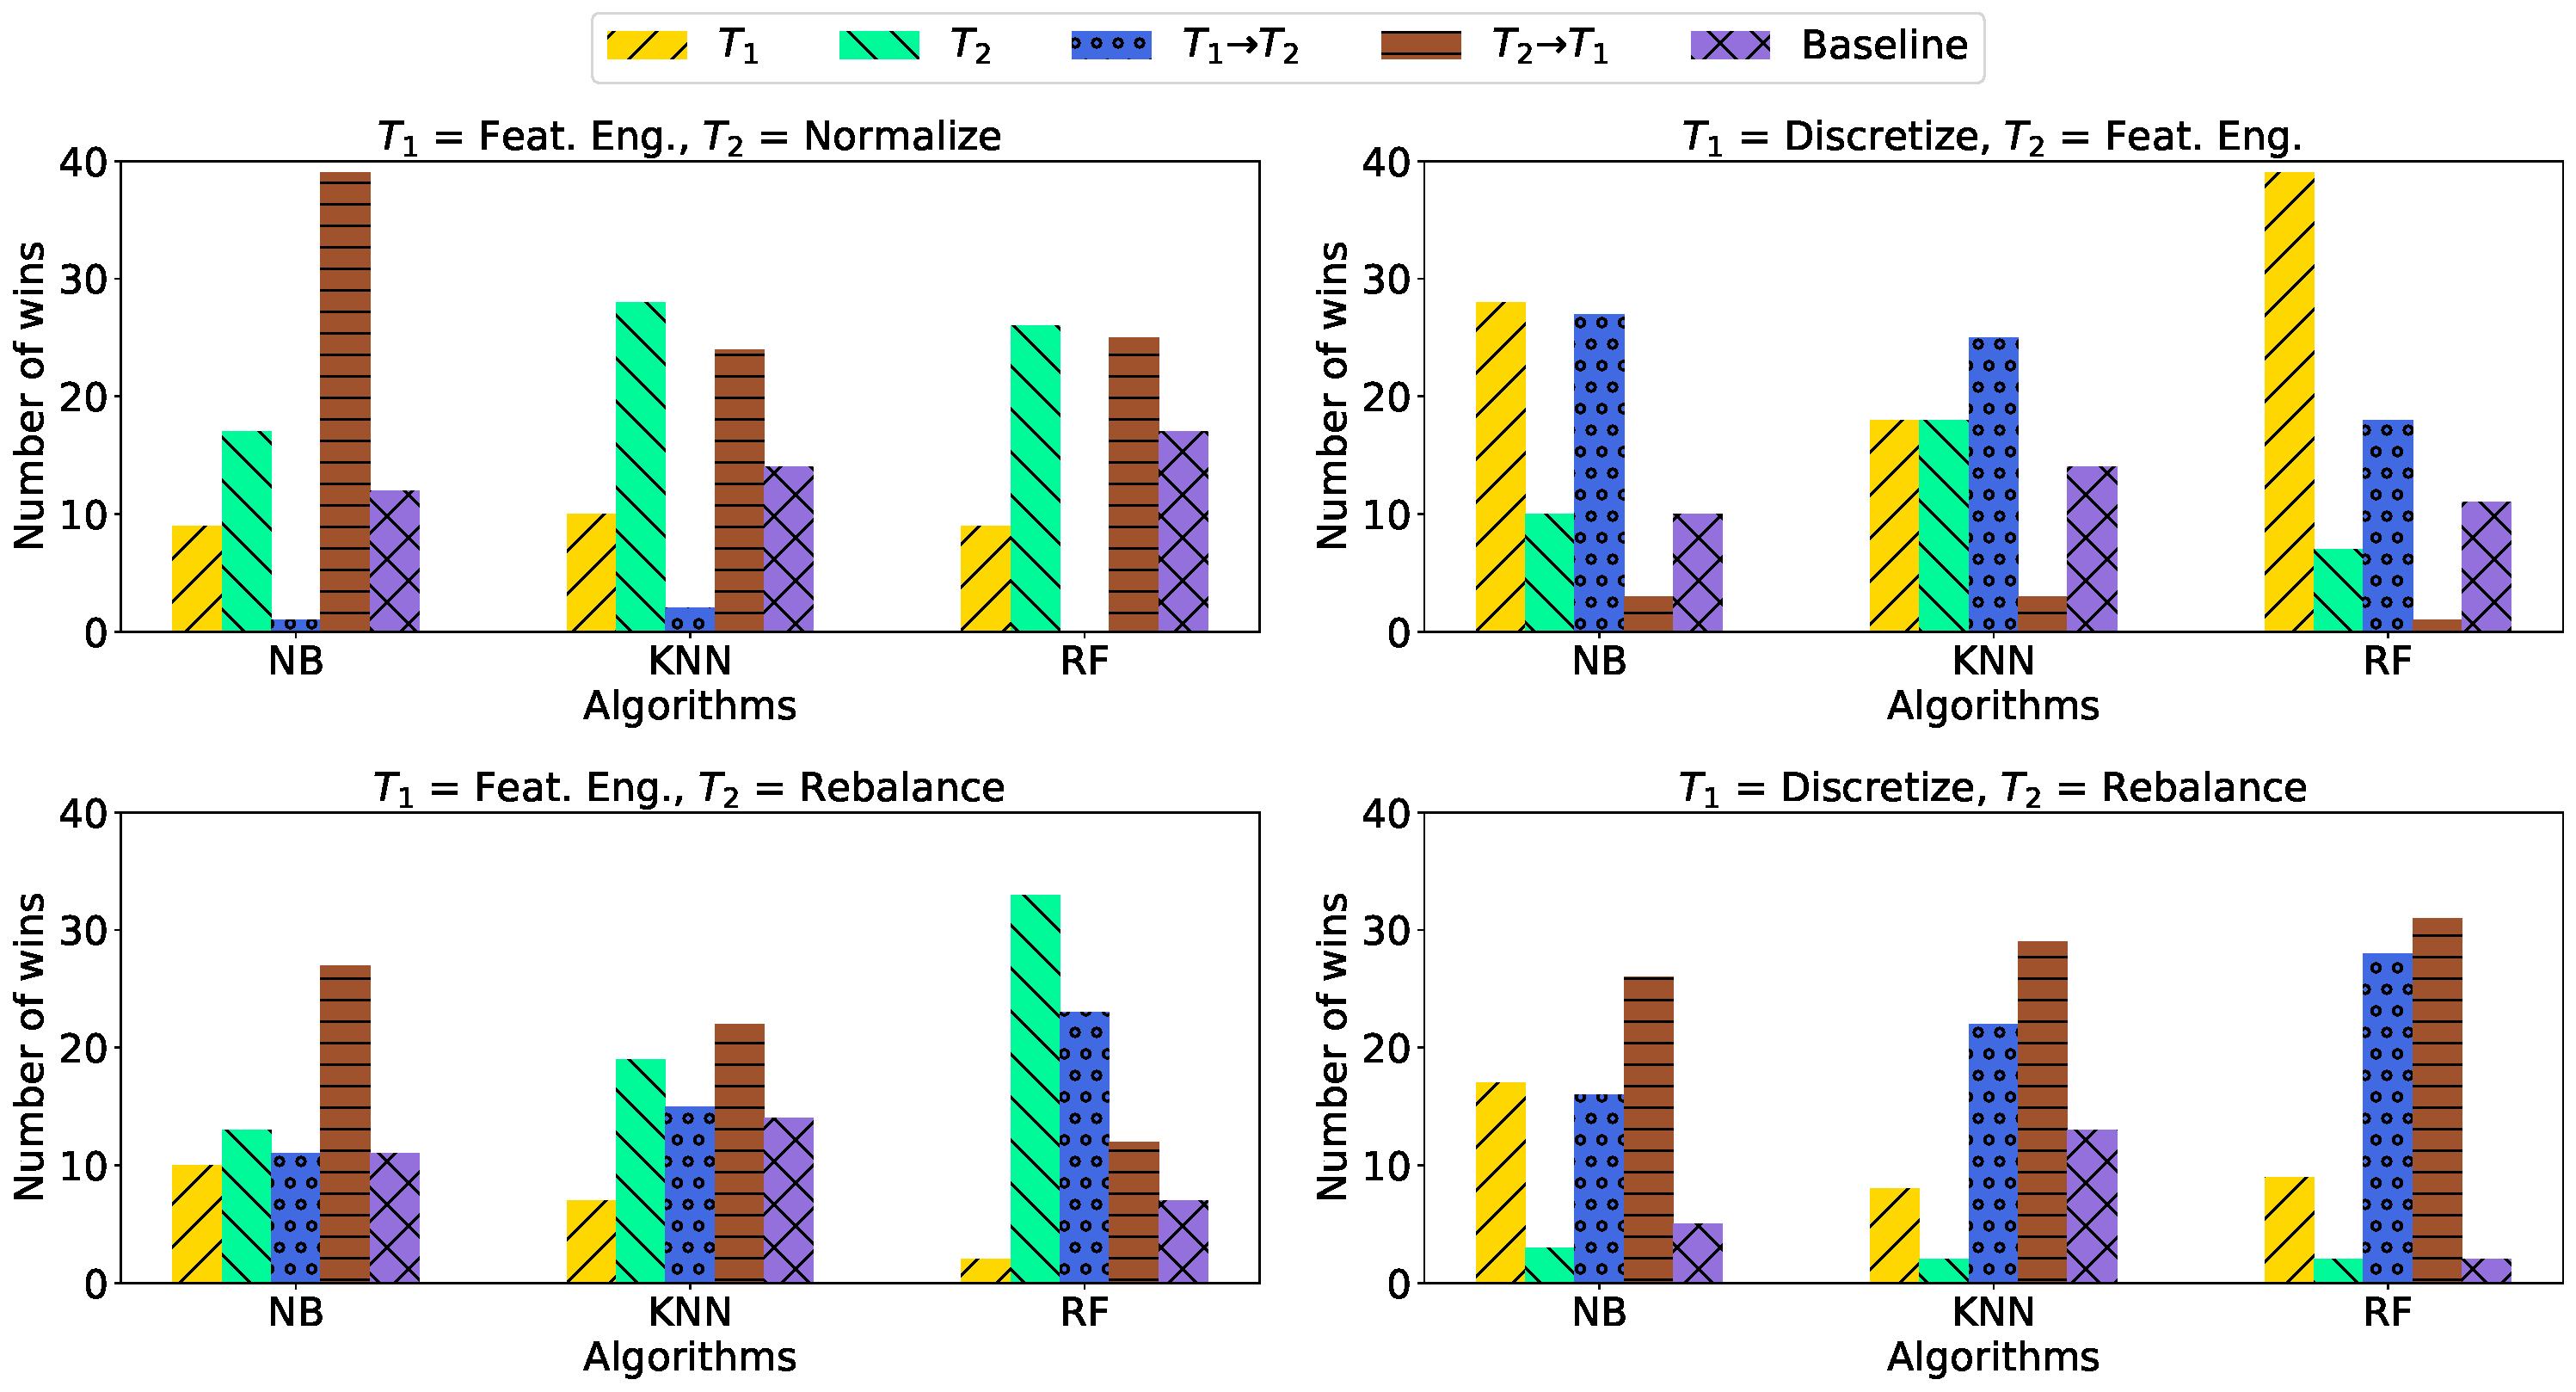
\includegraphics[width=1.0\textwidth]{part-automl/chapter-supervised/img-effective/experiments_results.pdf}
	\caption{Number of datasets for which a given pipeline prototype is declared the winner.}
	\label{fig:learned-rules-results}
\end{figure*}

To find a promising precedence order between a given pair of transformations, we propose Algorithm~\ref{alg:learned-rules}. 
To compute the impact of transformations, we first get the accuracy of the ML algorithm over the original non-transformed dataset (see line 1). %, which is used later for calculating the change in accuracy. 
Afterwards, for each precedence order between the pairs of transformations, we find both their optimized executable pipelines (i.e., using SMBO), and the accuracies of the ML algorithm (with default parametrisation) over the datasets transformed using the respective pipelines (see lines 2-3). Based on the comparison between the respective optimized pipelines, we get the winner in line 5. However, beforehand, in line 4, we perform a validity check. This is because when optimizing a pre-processing pipeline, SMBO may not instantiate a transformation with an operator at all (i.e., represented with a $\varnothing$ symbol).
Hence, given a pair of transformations, where one or both of them may not be instantiated, SMBO may generate 16 possible scenarios. They are listed in Table~\ref{tbl:validation-rules}, and make up the validation rules for Algorithm~\ref{alg:learned-rules} (see line 4). 

Briefly, if among the optimized pairs of transformations (same transformations but in reverse order) obtained from SMBO, one or both of them contain a $\varnothing$ operator, their results are considered valid, only if they have equal scores (i.e., a draw). This is because, if one has a higher score, it means that during the optimization phase it was more advantageous than the other, since it could find a configuration that should have been found by both of the pairs, given enough budget. In our SMBO runs, such invalid results account for less than 10\% and in those cases datasets are discarded from the study (see line 7). 

In particular, in Table~\ref{tbl:validation-rules}, the first two columns denote the pipeline instantiations for the respective pairs of transformations (i.e., $T_1\rightarrow T_2$ and $T_2\rightarrow T_1$). Next, \textit{Valid result} denotes the expected result when comparing the results of the pipelines in the same row. For instance, in the first row, if both transformations in the pipelines are not instantiated during the optimization, a valid result is a draw, and a \textit{Valid score} for the respective result is the baseline accuracy, and the \textit{Winner prototype} is the prototype that is in accordance with the expected result, which in this case is the Baseline (i.e., prototype consisting of only the ML algorithm, where no transformations are applied).

For the sake of another example, let us check row 2 in Table~\ref{tbl:validation-rules}. Running SMBO, the best result for the first pair is the pipeline $\varnothing \rightarrow \varnothing$, and for the second pair, the pipeline $T_2 \rightarrow \varnothing$. In this case, the comparison between the results of these pipelines should be equal (i.e., draw), and the score should be that of the baseline. Otherwise, if say, the score of the second pipeline was higher, it would mean that for the first pair, SMBO was not given enough time to find the pipeline with higher score (i.e., $T_2\rightarrow \varnothing$).
The same logic applies also for the other rows where a $\varnothing$ operator is involved.

\color{black}

\begin{example}
For the sake of this work, we considered three classification algorithms (i.e., \textit{NB}, \textit{RF},  \textit{KNN}) and 80 datasets from the OpenML repository. The datasets, were compiled from three OpenML benchmarks, namely, the OpenMLCC18 benchmark\footnote{\url{https://www.openml.org/s/99/data}}, the AutoML benchmark\footnote{\url{https://www.openml.org/s/271/data}}, and the Classification algorithms benchmark\footnote{\url{https://www.openml.org/s/1/data}}. For the final set, we filtered out datasets with more than 10\% of missing values --- not to include bias due to the heavy pre-processing we need to perform on top of them, and we filtered out the datasets with more than 5 million instances --- because of the computation time required to process them. As a result we obtained 60 datasets from the first benchmark, 17 from the second, and 3 more from the third to reach a total of 80 datasets. 

Given the proposed algorithm (i.e. Algorithm~\ref{alg:learned-rules}), we could try to learn the precedence of every pair of transformations, but would just be a waste of resources, because we can see in Table~\ref{tbl:rules}a and~\ref{tbl:rules}b, that some precedences are already decided for one reason or another. Hence, only pairs of transformations with a \texttt{0} for both directions (in both Table~\ref{tbl:rules}a and~\ref{tbl:rules}b) need to be studied further. That is, they make sense to be combined together, but a precedence order could not be determined through \textit{framework-related} or \textit{heuristic rules}. % for them. 
Thus, for instance, pairs involving Encoding are not considered in this phase, since for them an order is already imposed by the framework (see Table~\ref{tbl:rules}a).
To this end, the pairs of transformations we consider for the third precedence graph include only $\{F,N\}$, $\{F,D\}$, $\{F,R\}$, and $\{R,D\}$.

\begin{table}[t]
	\centering
	\footnotesize
	\begin{threeparttable}
		\caption{
			Binomial test for determining the order between pairs of transformations. 
		}
		\label{tbl:significance-test}
		\begin{tabular}{@{}cccccc@{}}
			\toprule
			%$T_1$ & $T_2$ & $T_1 \rightarrow T_2$ & $T_2 \rightarrow T_1$ & alpha & \begin{tabular}[c]{@{}c@{}}p-value\\ $H_0:\pi = \pi_0=0.8$\end{tabular} \\ \midrule
			$T_1$ & $T_2$ & $T_1 \rightarrow T_2$ & $T_2 \rightarrow T_1$ & alpha & p-value\\ \midrule
			$F$ & $N$ & 3 & 88 & 0.05 &  \textbf{0} \\
			$D$ & $F$ & 70 & 7 & 0.05 &  \textbf{0}  \\
			$F$ & $R$ & 49 & 61 & 0.05 & 8.53e-01 \\
			$D$ & $R$ & 66 & 86 & 0.05 & 9.38e-01 \\ \bottomrule
		\end{tabular}
		\begin{tablenotes}
		\centering
		\scriptsize
		\item$N$ - Normalization; $D$ - Discretization; $R$ - Rebalancing; $F$ - Feature Engineering. 
		\end{tablenotes}
	\end{threeparttable}
\end{table}
Applying Algorithm~\ref{alg:learned-rules}, we obtain a pro\-mising order for each pair of transformations considered. %(i.e., $\{F,N\}$, $\{F,D\}$, $\{F,R\}$, $\{R,D\}$). 
Since SMBO is a randomized algorithm we experimented with (i) running it several times splitting the budget, and (ii) running it only once with the entire budget. For the experiments considered, no significant differences where observed, therefore we opted for running it once with the entire budget (i.e., 200 seconds per run), which allows for more configurations to be visited in a single run. Aggregating all the results, Figure~\ref{fig:learned-rules-results} shows the number of datasets, for which a given prototype (see Table~\ref{tbl:validation-rules}, column \textit{Winner prototype} for the list of labels) is selected as the winner. For instance, for the pair $\{F,N\}$ (i.e., Feature Engineering, Normalization), the prototype winning in more datasets for \textit{KNN} and \textit{NB} is $N\rightarrow F$. This means that in general, better results are obtained if Normalization is applied before Feature Engineering. 

Next, only $N$ appears as first for \textit{RF} and second best for \textit{KNN} and \textit{NB}, which means that for many datasets, considering different algorithms, it results better to apply only Normalization without combining it with Feature Engineering. The third position is for $\varnothing\rightarrow \varnothing$, which means that for some datasets it is better not to apply any of the transformations (in any combination). The remaining prototypes winning in some datasets are $F$ (only Feature Engineering), and $F \rightarrow N$ (Feature Engineering preceding Normalization).  Finally, for three datasets, that are omitted from the figure, there were no winning pipelines (i.e., pipelines resulted in a draw).

Since our goal is to find the best order for a pair of transformations, we focus on the performances of the pipelines where both of the transformations are instantiated (i.e., $T_1\rightarrow T_2$ versus $T_2\rightarrow T_1$). To do this, we check whether the difference between the number of datasets where they each appear to win are statistically significant by running a binomial test assuming a theoretical probability of 0.5. The results are shown in Table~\ref{tbl:significance-test}.
In summary, the results from Table~\ref{tbl:significance-test} indicate that, with 95\% confidence we can assume that for the pair $\{F,N\}$, $N\rightarrow F$ performs better than $F\rightarrow N$, hence Normalization should precede Feature Engineering. On the other hand, for $\{D,F\}$, $D\rightarrow F$ performs better than $F\rightarrow D$, hence Discretization should precede Feature Engineering. Finally, for the remaining transformations, $\{F,R\}$ and $\{R,D\}$, a precedence order can not be pre-assumed since the results obtained are not significant. 
Using these results, we create the \textit{Promising precedence} adjacency matrix shown in Table~\ref{tbl:rules}c, where as one can observe, precedence edges are introduced for $\{N,F\}$ and $\{D,F\}$, but no edges exist neither for $\{F,R\}$, nor for $\{R,D\}$. 
\end{example}

\paragraph{Cross-validation}
\label{ssec:learned-rules-validation}
After running Algorithm~\ref{alg:learned-rules} to empirically find a winner between two pairs of transformations, we may obtain a different distribution of the number of wins for the pairs, depending on the datasets considered. To show that the results obtained with the initial set of datasets are generalizable, we propose to perform an additional cross-validated experiment, where the set of datasets considered can be randomly split into many folds. Then, for each fold, the results can be compared to the rest, with the aim of checking whether the distributions are similar. This check can be done via a significance test (e.g., chi-square). To this end, if the distributions between the folds are similar, it means that the obtained results are independent of the datasets considered, since no matter the combination of the datasets, the results are the same and thus generalizable.


\color{black}

\begin{example}
In our use case, to show that the results do not depend on the datasests selected, we re-run the experiments (i.e., 10-times each), but this time splitting the datasets into 4-folds. The goal was to check if the results of the precedence orders from the different folds (i.e., for each experiment considering a randomly different set of datasets) are similar between them (i.e., follow the same distributions).
To confirm this hypothesis, we perform a chi-square test between the results (precedence orders) obtained in a single fold in comparison to the three remaining folds, hence comparing 25\% of the datasets to the rest. 
In particular, to confirm the hypothesis, we need to find results that accept the null hypothesis of the chi-square test which states that "there is no significant difference between the distributions". To do that, sticking to the 95\% confidence interval, we need to look for p-values greater than 0.05. That is, the higher the p-values, the more we accept the null hypothesis, the more similar the distributions. Looking at the p-values we found out that they were all much higher than 0.05. Specifically, the scores of the chi-square tests of the folds (one fold compared to the rest) are averaged and, after having repeated this procedure 10 times, instead of using a table we depict the 10 averaged p-values using box-plots in Figure~\ref{fig:10-times-4-cv}.
We conclude that, for both of the rules (i.e.,  $F\rightarrow N$ and $F\rightarrow D$), the significance test indicates a compliance between the new results (Figure~\ref{fig:10-times-4-cv}) and those illustrated above (Table~\ref{tbl:significance-test}).



\begin{figure*}[!t]
	\centering
	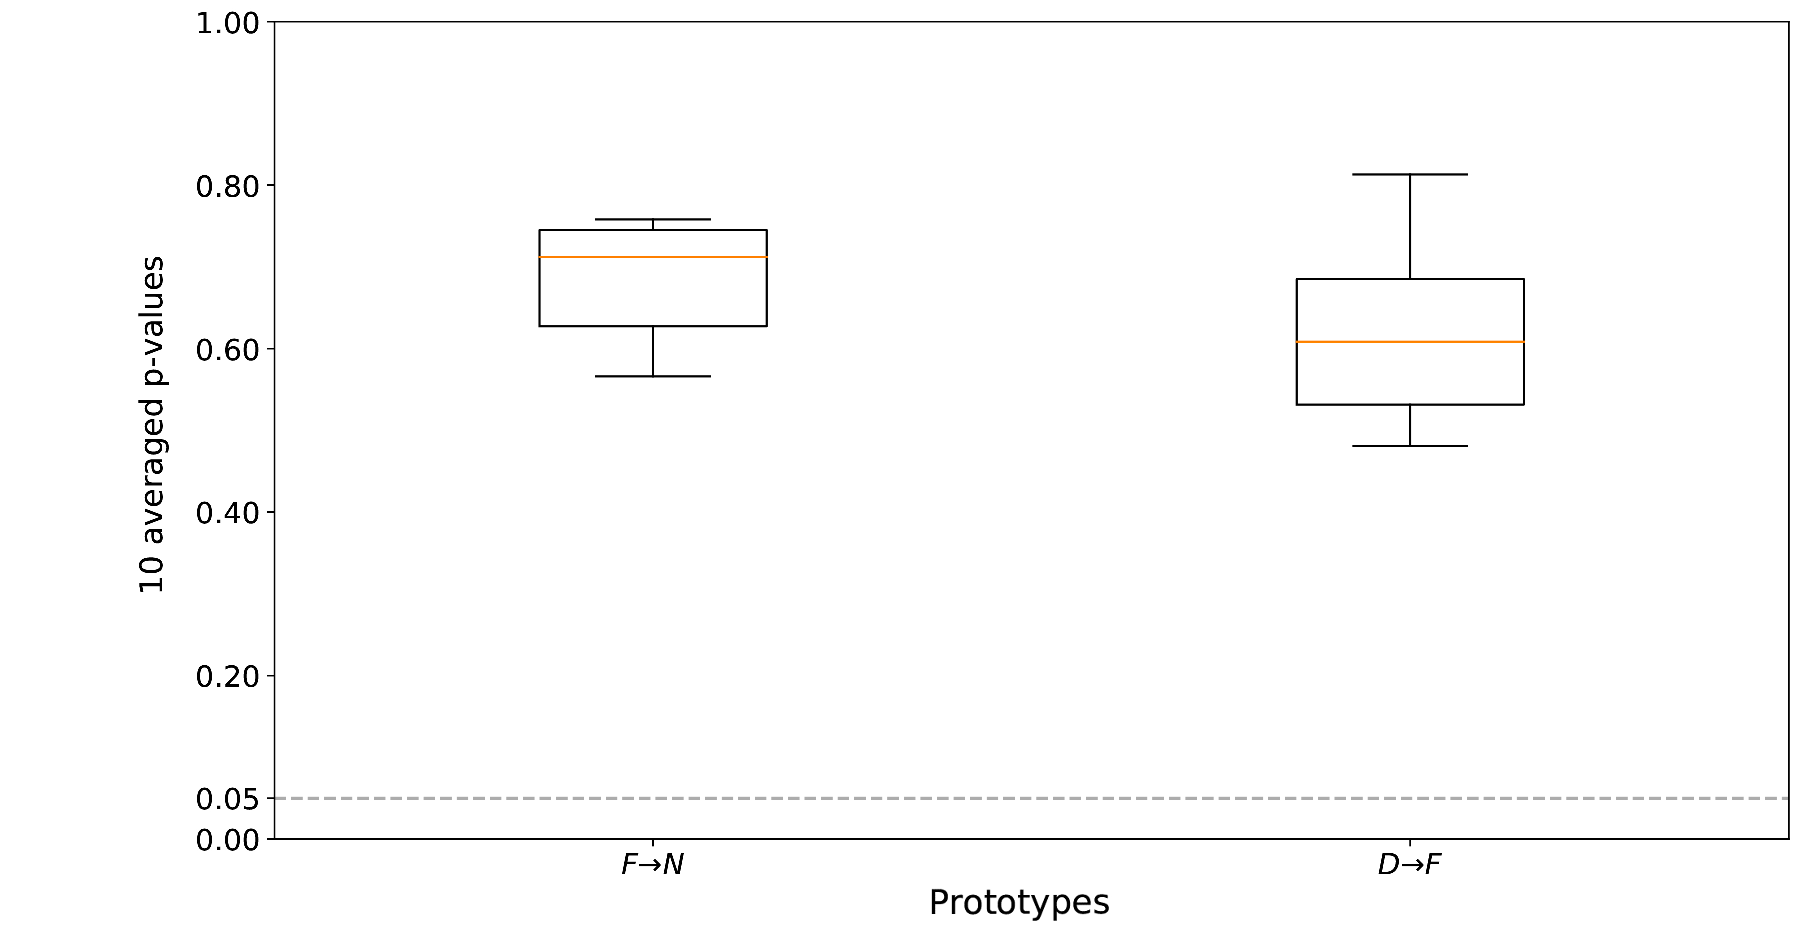
\includegraphics[width=0.9\textwidth]{part-automl/chapter-supervised/img-effective/10_times_4_folds_cv.pdf}
	\caption{The distribution of the p-values obtained after repeating the chi-square test for 10 times, for the 10 times 4-fold cross-validation.}
	\label{fig:10-times-4-cv}
\end{figure*}

\begin{table}[b]
	\caption{
		Union of rules from Table~\ref{tbl:rules}. $\boldsymbol{E}$ - Encoding; $\boldsymbol{N}$ - Normalization; $\boldsymbol{D}$ - Discretization; $\boldsymbol{I}$ - Imputation; $\boldsymbol{R}$ - Rebalancing; $\boldsymbol{F}$ - Feature Engineering \texttt{1} - an edge exists, \texttt{0} - edge does not exist, \texttt{X} - the combination is meaningless.
	}
	\renewcommand{\arraystretch}{0.3}
	\footnotesize
	\centering
	\label{tbl:rules-union}
	\begin{threeparttable}
		\begin{tabular}{@{}lcccccc}
			\toprule
			& $\boldsymbol{E}$ & $\boldsymbol{N}$ & $\boldsymbol{D}$ & $\boldsymbol{I}$ & $\boldsymbol{R}$ & $\boldsymbol{F}$
			\\	\cmidrule[.1em]{1-7}
			$\boldsymbol{E}$ & \cellcolor{gray!25} & \texttt{1} & \texttt{1} & \texttt{0} & \texttt{1} & \texttt{1} \\	\cmidrule[.1em]{1-7}
			$\boldsymbol{N}$ & \texttt{0} & \cellcolor{gray!25}  & \texttt{X} & \texttt{0} & \texttt{1} & \texttt{1} \\	\cmidrule[.1em]{1-7}
			$\boldsymbol{D}$ & \texttt{0} & \texttt{X} & \cellcolor{gray!25} & \texttt{0} & \texttt{0} & \texttt{1} \\	\cmidrule[.1em]{1-7}
			$\boldsymbol{I}$ & \texttt{1} & \texttt{1} & \texttt{1} & \cellcolor{gray!25}  & \texttt{1} & \texttt{1} \\	\cmidrule[.1em]{1-7}
			$\boldsymbol{R}$ & \texttt{0} & \texttt{0} & \texttt{0} & \texttt{0} & \cellcolor{gray!25}  & \texttt{0} \\	\cmidrule[.1em]{1-7}
			$\boldsymbol{F}$ & \texttt{0} & \texttt{0} & \texttt{0} & \texttt{0} & \texttt{0} & \cellcolor{gray!25} \\	\cmidrule[.1em]{1-7}
		\end{tabular}
	\end{threeparttable}
\end{table}

\begin{figure}
\begin{floatrow}
\ffigbox{
    \includegraphics[clip, trim=2.5cm 23cm 10.5cm 2cm,width=0.5\textwidth]{part-automl/chapter-supervised/img-effective/graph.pdf}
}{
  	\caption{Precedence graph generated from Table~\ref{tbl:rules-union}. $E$ - Encoding; $N$ - Normalization; $D$ - Discretization; $I$ - Imputation; $R$ - Rebalancing; $F$ - Feature Engineering. }
}
\capbtabbox{
\begin{tabular}{@{}ll}
			\toprule
			ID& Pipeline prototype                                             \\ \toprule
			1&{\color[HTML]{000000} $I\rightarrow E\rightarrow N \rightarrow R\rightarrow F$} \\
			2&{\color[HTML]{000000} $I\rightarrow E\rightarrow N \rightarrow F\rightarrow R$} \\
			3&{\color[HTML]{000000} $I\rightarrow E\rightarrow R \rightarrow D\rightarrow F$} \\
			4&{\color[HTML]{000000} $I\rightarrow E\rightarrow D \rightarrow R\rightarrow F$} \\
			5&{\color[HTML]{000000} $I\rightarrow E\rightarrow D \rightarrow F\rightarrow R$} \\
			\bottomrule
		\end{tabular}
}{
  	\caption{Effective pipeline prototypes generated from Figure~6. $E$ - Encoding; $N$ - Normalization; $D$ - Discretization; $I$ - Imputation; $R$ - Rebalancing; $F$ - Feature Engineering.
	}
}
\end{floatrow}
\end{figure}



\iffalse

\begin{figure}[t]
	\centering
	\begin{tikzpicture}[]
	\begin{scope}[xshift=10.5cm,yshift=-5cm,thick,
	node distance=1.0cm,on grid,>=stealth',
	block/.style={rectangle,draw,fill=cyan!20},
	vertex/.style={circle,draw,fill=orange!40},
	i/.style={circle,draw,fill=yellow!40},
	e/.style={circle,draw,fill=blue!25},
	f/.style={circle,draw,fill=orange!40},
	r/.style={circle,draw,fill=cyan!40},
	n/.style={circle,draw,fill=green!40},
	d/.style={circle,draw,fill=red!40}]
	decision/.style={diamond,draw,fill=white!40}]
	%layer0
	\node [i]	 (ti0) {$I$};
	\node [e]	 (te0)	[right=of ti0,xshift=1.6cm,yshift=1.3cm]	{$E$} edge [<-] (ti0);
	\node [n]	 (tn0)	[right=of te0,xshift=0.5cm,yshift=1.8cm]	{$N$} edge [<-] (te0);
	\node [d]	 (td0)	[right=of te0,xshift=0.5cm,yshift=-1.3cm]	{$D$} edge [<-] (te0);
	\node [r]	 (tr0)	[right=of tn0,xshift=1.6cm,yshift=-1.2cm]	{$R$} edge [<-] (tn0);
	\node [f]	 (tf0)	[right=of tn0,xshift=1.6cm,yshift=-2.3cm]	{$F$} edge [<-] (tn0);
	\path [->,draw,thick] (ti0) -- (tn0); 
	\path [->,draw,thick] (ti0) -- (tr0);
	\path [->,draw,thick] (ti0) -- (tf0);
	\path [->,draw,thick] (ti0) -- (td0);
	\path [->,draw,thick] (te0) -- (tr0);
	\path [->,draw,thick] (ti0) -- (tf0);
	\path [->,draw,thick] (td0) -- (tf0);
	\path [->,draw,thick] (tn0.285) -- (td0.75);
	\path [->,draw,thick] (td0.105) -- (tn0.255);
	\end{scope}
	\end{tikzpicture}
	\caption{Precedence graph generated from Table~\ref{tbl:rules-union}. $E$ - Encoding; $N$ - Normalization; $D$ - Discretization; $I$ - Imputation; $R$ - Rebalancing; $F$ - Feature Engineering.
	}
	\label{fig:precedence-graph}
\end{figure}


\begin{table}[t]
	\caption{Effective pipeline prototypes generated from Figure~6%\ref{fig:precedence-graph}
	. $E$ - Encoding; $N$ - Normalization; $D$ - Discretization; $I$ - Imputation; $R$ - Rebalancing; $F$ - Feature Engineering.
	}
	\footnotesize
	\label{tbl:effective-pipelines}
	\begin{center}
		\begin{tabular}{@{}ll}
			\toprule
			ID& Pipeline prototype                                             \\ \toprule
			1&{\color[HTML]{000000} $I\rightarrow E\rightarrow N \rightarrow R\rightarrow F$} \\
			2&{\color[HTML]{000000} $I\rightarrow E\rightarrow N \rightarrow F\rightarrow R$} \\
			3&{\color[HTML]{000000} $I\rightarrow E\rightarrow R \rightarrow D\rightarrow F$} \\
			4&{\color[HTML]{000000} $I\rightarrow E\rightarrow D \rightarrow R\rightarrow F$} \\
			5&{\color[HTML]{000000} $I\rightarrow E\rightarrow D \rightarrow F\rightarrow R$} \\
			\bottomrule
		\end{tabular}
	\end{center}
\end{table}
\fi

\end{example}
\subsubsection{Effective pipeline prototypes}
\label{ssec:composition}
In this task we foresee the composition of the previously defined rules (i.e., for the pairs of transformations), to generate the final set of rules that would allow to compose longer chains --- consisting of more than two transformations. This is when we resolve the inconsistencies and also define precedences for the pairs of transformations that may not have any precedence defined already --- in that case, we basically take into account all the permutations. This step allows to finally generate the possible effective pipeline prototypes. 

\begin{example}
To generate the final pipeline prototypes, in this step we combine all the matrices generated by the previous steps. That is, we take the union of the edges (represented by \texttt{1}'s) from the matrices in Table~\ref{tbl:rules} (a,b,c), and create a new final adjacency matrix, shown in Table~\ref{tbl:rules-union}. This is the matrix that will allow us to generate the final effective pipeline prototypes. 

Observing the table, one can realize that for pairs $\{F,R\}$ and $\{R,D\}$, no precedence edges exist. This means that these pairs are somewhat equally relevant from either direction (any order), and thus when generating the final prototypes, both options should appear.

For a better reading, in Figure~6, we visualize Table~\ref{tbl:rules-union} in form of a graph, where nodes represent the kinds of transformations and the directed edges represent a precedence order between them.
Out of the graph, we generate the final pipeline prototypes by taking all the maximum length variations (ordered arrangements without repetition) of the nodes, respecting the precedence rules (i.e., not contradicting the direction of existing edges). The result is the set of five pipeline prototypes shown in Table 6. This set consisting of \textit{compatible}, \textit{meaningful} and \textit{promising} pairs of transformations is the set of recommended \textit{effective pipeline prototypes}.
\end{example}

\color{black}
\subsubsection{Meta-learning rules}
\label{ssec:meta-learning}
Once the pipeline prototype is constructed, that is, the order between the kinds of transformations is defined, what follows is the instantiation of transformations with the physical operators. For that, one can rely completely on the optimization algorithm, and let the algorithm choose the right operators. However, given the way optimization algorithms work (e.g., SMBO) --- successively finding better and better instantiations, there is a cold-start problem, where in the beginning, the algorithm does not have enough information in order to come up with the most promising initial instantiations, and a wrong choice may affect the optimization process. 
\paragraph{Exploratory analysis}
Given the availability of the experimental SMBO executions (executed in an exhaustive manner, considering all the pipeline prototypes), one can perform an exploratory analysis with the aim of removing useless prototypes, pipelines or operators. Hence, further tweaking the search space. In particular, starting from the highest level, that of prototypes, then going to the physical pipelines, and finally to the actual operators inside the pipeline, one can analyze if:

\begin{itemize}
    \item there exist some combination of transformations in the form of prototypes (see Table~\ref{tbl:pipeline-enumeration} for the exhaustive list of prototypes), that are generally useless (i.e., in terms of their impact to the final accuracy), and thus can be discarded a priori in order to reduce the search space, 
    \item there are some physical pipelines that are consistently chosen more often than others by the optimization algorithm, meaning that they are more useful than others,
    \item within the physical pipelines, some transformations are chosen more often than others, meaning that they provide more positive impact. 
    \end{itemize}

\begin{example}
We performed the above-mentioned analysis to our use case, but it did not lead to any conclusive or significant results. In particular, as shown in Figure~\ref{fig:prototypes-impact}, we could not find any useless prototypes --- not positively impacting the final accuracy, that could be discarded a priori from the potential list of prototypes.
Actually, as we will show in Section~\ref{ssec:eval-universal-pipeline}, all of them lead to the best in one case or another, which does not mean the epsilon improvement some provide is worth the search cost you incur in considering them (but this more in-depth analysis is done later).
Next, as shown in Figure~\ref{fig:pipeline-frequency}, there were no physical pipelines shown to be more useful --- hence more often selected, than others. Even if $N \rightarrow R$ is clearly above, it barely reaches 30\% in KNN.
 Finally, observing Figure~\ref{fig:transformation-frequency}, it is clear that some kinds of transformations are chosen more often, but looking closely (i.e., the shaded bars), it is not clear which operator brings more benefit. For instance, Normalization is present in 90\% of the pipelines, but it is not easy to distinguish which kind of Normalization (i.e., actual operator) is more beneficial.
For this, we need more complex rules or guidelines that may help in finding the right operator to use. 
\end{example}

\begin{figure*}[!t]
	\centering
	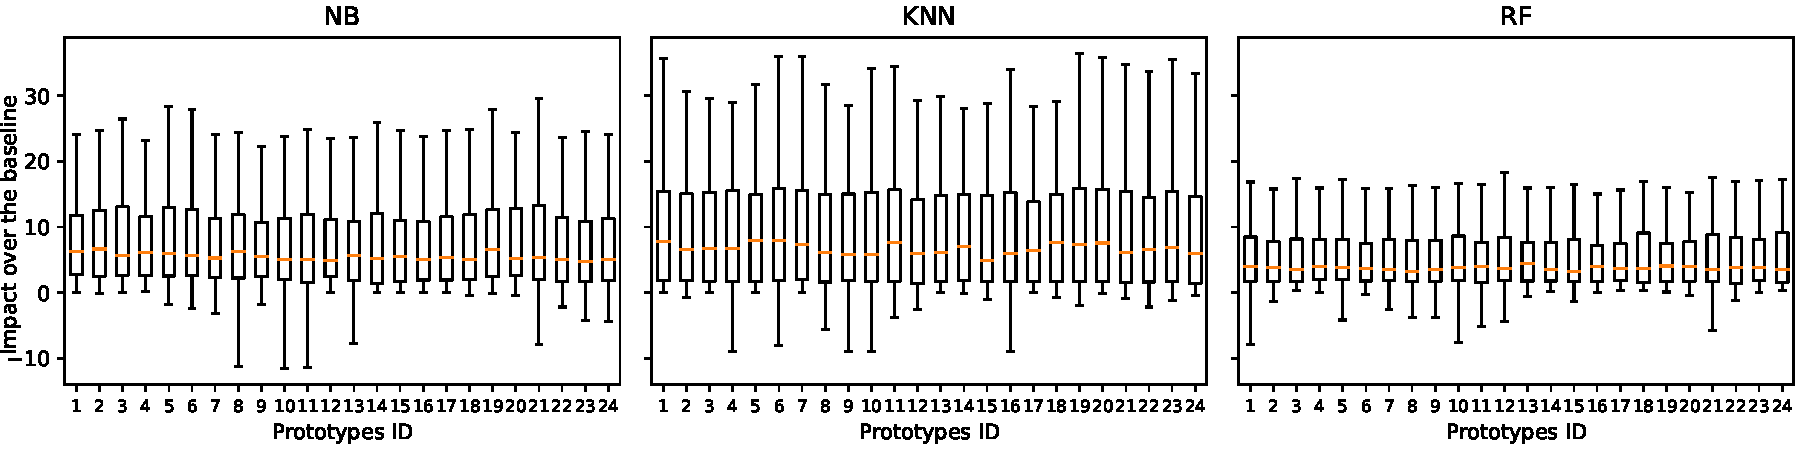
\includegraphics[width=1.0\textwidth]{part-automl/chapter-supervised/img-effective/prototypes_impact.pdf}
	\caption{The impact of the different pipeline prototypes over the baseline (i.e., when no transformation is applied).}
	\label{fig:prototypes-impact}
\end{figure*}

\begin{figure*}[!h]
	\centering
	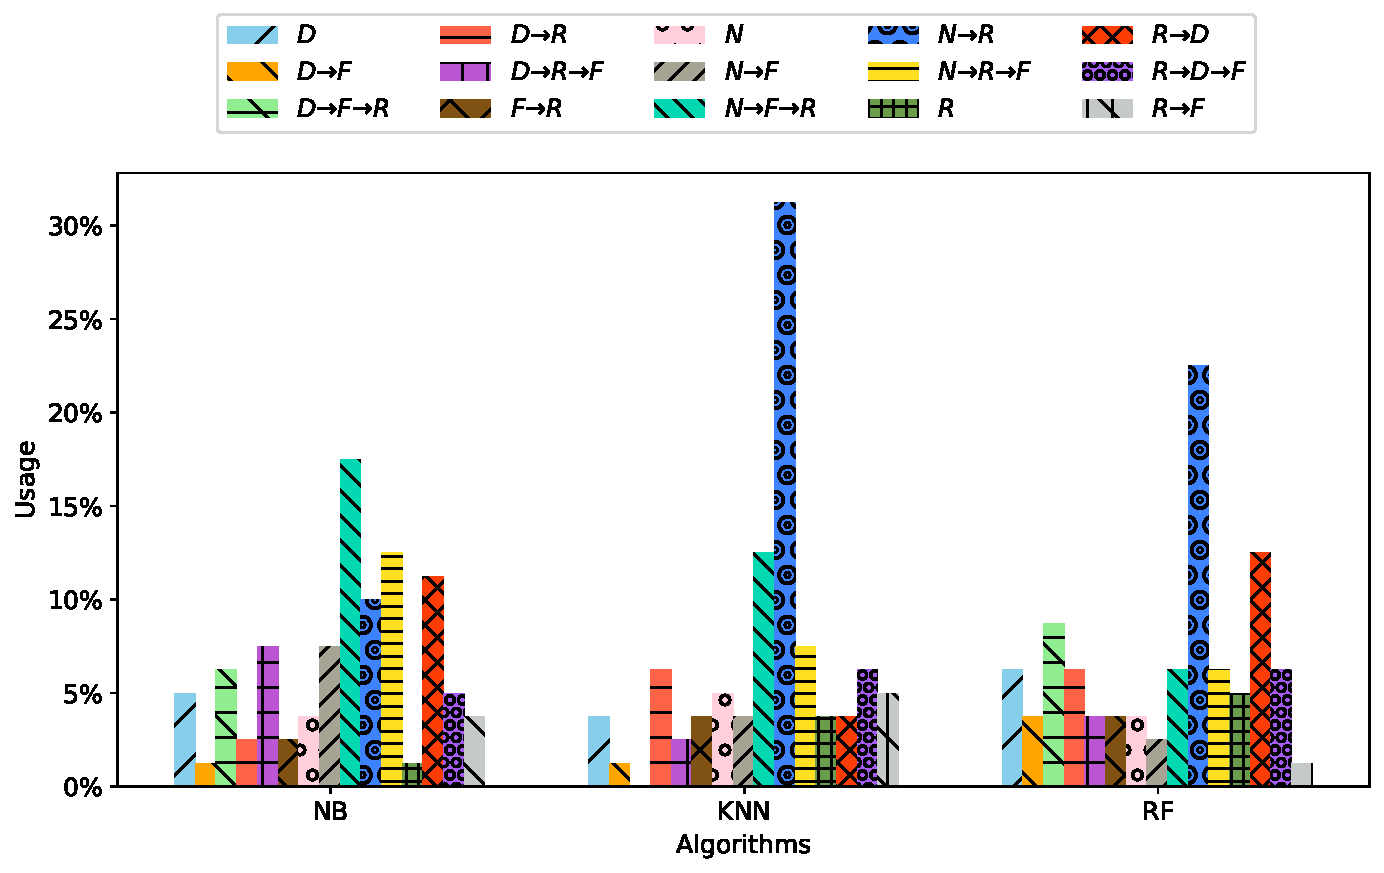
\includegraphics[width=1.0\textwidth]{part-automl/chapter-supervised/img-effective/pp_pipeline_study2.pdf}
	\caption{Percentage of use of the different physical pipelines.}
	\label{fig:pipeline-frequency}
\end{figure*}

\begin{figure*}[!h]
	\centering
	\includegraphics[width=0.7\textwidth]{part-automl/chapter-supervised/img-effective/pp_pipeline_study_grouped.pdf}
	\caption{Percentage of use of a transformation in a physical pipeline.}
	\label{fig:transformation-frequency}
\end{figure*}

\subsubsection{Meta-learning}
\color{black}
To mitigate the red cold-start problem, we propose to perform meta-learning (shown in Figure~\ref{fig:methodology}), where we intend to use the knowledge extracted from historical data in order to devise rules that may help the optimization algorithm in its initial phase. 
Meta-learning is the process of `learning on top of learning', or learning a model using historical data from ML experiments. Traditionally, it has been used for predicting the performance (e.g., predictive accuracy) of an algorithm on a given dataset. That is, given some historical runs of the performance of classification algorithms over various datasets (i.e., meta-database: consisting of datasets characteristics as predictive variables and the performance of the classification algorithm as the response variable), one can learn a model (i.e., meta-model), that is able to predict the performance of a given classification algorithm on a new dataset~\cite{Brazdil04Book}. Lately, this technique has been extended in order to predict the impact of transformations over the performance of classification algorithms and thus rank transformations based on their impact~\cite{Bilalli17AMCS, presistant18CSI, presistant19DKE}. The same idea can be applied for learning the best operator for a given transformation.
That is, through meta-learning one can learn the intrinsic relationship between dataset characteristics and the operator performance, and thus come up with rules that are not obvious and are effective at the time of instantiating a transformation. 
The main idea is to build a model, that is able to predict the operator for a certain kind of transformation, given the meta-features extracted from the dataset considered for the optimization. This translates to answering the following question: ``given that we know the dataset characteristics and having selected a certain kind of transformation (e.g., missing value imputation), what is the optimal physical algorithm (see Table~\ref{tbl:transformations}) we need to select, to obtain the highest improvement possible in terms of classification accuracy (i.e., when the classification algorithm is applied over the transformed dataset)?".  In particular, the model can generate a set of complementary rules that help in the optimization, providing a good starting instantiation for some of the transformations in the prototype.

To train the model we need a meta-dataset that can be  (i) generated through optimization algorithms (e.g., SMBO executions), (ii) generated manually through simple evaluations of classification algorithms over transformed datasets, or (iii) assumed already given (e.g., OpenML). 

Given a meta-dataset, we propose to learn to predict the best instantiation (operator) for a given transformation, where among the classes we can include the class \texttt{None} too. This means that one of the possible predictions is to not instantiate a transformation at all, hence remove it from the pipeline.

\begin{example}
Our training dataset (sometimes referred to as `meta-database' or `meta-dataset') for the meta-learning is compiled through SMBO runs on the OpenML datasets (see Section~\ref{ssec:rules-learned:algorithm}). That is, we first extract the dataset characteristics/profiles (i.e., number of features, number of instances, number of missing values, etc), and then by applying SMBO optimization, on classification algorithms and pre-processing pipelines (as explained in Section~\ref{ssec:composition}), for each dataset, we retrieve the evaluations (i.e., predictive accuracy) of the algorithms over the optimized pipelines. This gives us the presumably optimal physical pipelines and their impact on the accuracy of the learning algorithms for each dataset at hand. Given such information, our aim is to now save time and improve the instantiation of the operators for each transformation considered in the prototype. 

We trained several different Conditional Inference Trees \cite{ctree} because they produce models that can be easily read and interpreted.
Specifically, the independence of each variable (meta-features in our case) with the class (operator of a specific transformation) is tested through a statistical test. 
The split is made on the variable with the lowest p-value. 
We report the p-value too, so that it can be seen how strong the association is (i.e., why that variable was chosen).
We stick with the p-value threshold of 0.05, and devise a rule from any branch of the tree that is within the threshold. In the following, we describe the rules obtained within the selected significance threshold.

\textbf{Rules for Feature Engineering}. The available operators in Scikit-learn for Feature Engineering (see Table~\ref{tbl:transformations}) are: \texttt{PCA} (Principal Component Analysis), \texttt{Feature Selection} (Select K Best), \texttt{Both} (PCA + Select K Best), and \texttt{None}. The tree generated for the Feature Engineering transformation is shown in Figure~\ref{fig:features-meta-learning:feature-engineering}. The leaves show the selected operator frequency. For the sake of simplicity, we do not consider the union of PCA and Select K Best as an operator per se, instead we distribute that contribution to the two operators that compose it.
Observe that there is a strong correlation between the Feature Engineering operator and the entropy of the class attribute.
Indeed, such a meta-feature achieved a p-value smaller than 0.001.
We can clearly read that if the Class Entropy is low, then \texttt{Feature Selection} is way more chosen than the other options (see Node 2).
Recall that the entropy of an attribute is a measure of how much disorder there is among its instances.
The less is that value, the easier is the classification problem.
As a consequence, it is reasonable to think that the easier the classification problem is, the more likely is the fact that the class can be described by a low number of features.
Hence, the \texttt{Feature Selection} technique can be successfully applied.
Conversely, Node 5 shows that, when the Class Entropy is high, it is better to not apply any Feature Engineering operator.
As a matter of fact, a high value of Class Entropy involves a high number of classes and/or few instances per class, hence a really difficult problem.
In such cases, reducing the dimensionality of the dataset does not lead to any improvement.
Finally, when the Class Entropy is in between, there is no clear winner, and thus other non-obvious factors may affect the choice of the operator.

\textbf{Rules for Rebalancing}. As for Rebalancing, the operators considered from the imblearn\footnote{\url{https://pypi.org/project/imbalanced-learn}} library are: \texttt{Near Miss}, \texttt{SMOTE}, and \texttt{None}. %\joseph{the rebalance implementations are of actually from imblearn (imbalanced-learn)}
The first is an undersampling algorithm which randomly eliminates the samples from the larger class.
Instead, the second is an oversampling technique that creates samples of the minority class, as a linear combination of them.
As shown in Figure~\ref{fig:features-meta-learning:rebalancing}, the meta-feature Majority Class Percentage has a p-value of 0.014.
This can be read as, in case of an unbalanced class problem (i.e., Node 3: Majority Class Percentage greater than 56), an oversampling of the minority class(es) is preferred to a downsampling of the majority one(s).
However, when the Majority Class Percentage is smaller than 56\%, the situation is not that clear, and there is no technique that is applied significantly more often than the rest; they are close to each other.
Therefore, it is difficult to understand which problems (which dataset characteristics do they have) belong to Node 2.
In summary, when the majority class has no more than 56\% , it implies that it is an unbalanced class, and as mentioned above, SMBO tends to choose the same operator. However, when the majority class has less than 56\%, it may imply that: (i) there are just two classes and the problem counts as a balanced problem, so no operator needs to be applied, or (ii) it is a multi-class problem, and thus there is no clear winner in terms of operators. 
\end{example}


\subsubsection{Prototype instantiation}

The prototypes from the top flow and the meta-lerning rules from the bottom flow (if the optimization framework permits), are finally fed to the final step which deals with the instantiation and optimization of the prototypes. In this task we run an optimization algorithm that is executed until an optimal pipeline is found.

\begin{example}
 In our final execution, we run SMBO to find a suitable instantiation for the suggested prototypes. The simple but not obvious meta-learning rules, even though not included in our final execution, because of the implementation considered (i.e., HyperOpt), can potentially be used to ease the cold-start problem. 
\end{example}

\begin{figure*}[!h]
	\centering
	\includegraphics[clip, trim=1.0cm 0.4cm 1cm 1cm,width=1\textwidth]{part-automl/chapter-supervised/img-effective/tree-FE.pdf}
	\caption{Conditional Inference Tree built for the \textit{Features Engineering} transformation.}
	\label{fig:features-meta-learning:feature-engineering}
\end{figure*}

\begin{figure*}[!h]
	\centering
	\includegraphics[clip, trim=5.8cm 0.4cm 5.05cm 3.5cm,width=0.65\textwidth]{part-automl/chapter-supervised/img-effective/tree-RE.pdf}
	\caption{Conditional Inference Tree built for the \textit{Rebalancing} transformation.}
	\label{fig:features-meta-learning:rebalancing}
	\end{figure*}

%In our recent future work we aim to extend HyperOpt with the functionality of incorporating mechanisms that ease the cold start problem. The technique of using meta-learning for the cold-start problem has for instance been applied in \cite{Feurer15AAAI}, however the overall method lacks the initial part of finding promising pipeline prototypes (i.e., works over single transformations), meaning that the instantiation via meta-learning may occur in the wrong place (not the optimal prototype), resulting into a solution that is a local optimum. 


\subsection{Evaluation}
\label{ssec:evaluation}

The aim of our experimental study is three-fold:
\begin{enumerate}
    \item Check whether there exists a universal pipeline prototype that works best for any classification problem considered  (i.e., dataset and ML algorithm) (Section~\ref{ssec:eval-universal-pipeline}).
    \item Assess and compare the performance of the effective pipelines constructed using our method against the set of exhaustively generated pipeline prototypes (Section~\ref{ssec:eval-our-vs-rest}).
    \item Assess and compare the impact of dedicating a portion of the optimization time to the effective pipelines constructed using our method, with the impact of using the whole optimization time for the hyper-parameters of the ML algorithm (Section~\ref{ssec:eval-dpso-vs-cash}).
\end{enumerate}

The experiments were performed on an Intel Core i7 machine with 12 cores, running at 3.20 GHz with 64 GB of main memory. As a platform for running the SMBO optimization algorithm we use HyperOpt. Furthermore, the datasets used in the experiments are the ones from the OpenML repository (see Section~\ref{sec:rules-learned:algorithm}). Finally, the classification algorithms considered are \textit{NB}, \textit{KNN}, and \textit{RF}. All the experiments for a single algorithm, on average took approximately two weeks\footnote{The source code and the datasets for reproducing the experiments can be found in 
\href{https://github.com/josephgiovanelli/effective\_preprocessing\_pipeline\_evaluation}{https://github.com/josephgiovanelli/effective\_preprocessing\_pipeline\_evaluation}}.

\subsubsection{Universal pipeline prototype}
\label{ssec:eval-universal-pipeline}
The goal of this experiment is to demonstrate the difficulty of blindly finding the right pipeline prototype (i.e., without considering any meaningful or promising precedence).
In Table~\ref{tbl:pipeline-enumeration}, we list the exhaustive set of pipeline prototypes generated considering the compatible precedence graph in Table~\ref{tbl:rules}a (i.e., 24 compatible permutations). In a real scenario, this number would be too high for splitting the time budget in order to optimize them. 
Yet, for the sake of this experiment, we exhaustively optimize all the prototypes, for each dataset. Thus, for each pipeline prototype and for each dataset, the SMBO algorithm is configured to assign a 200 seconds time budget to the phase of instantiating and optimizing the pipeline prototype, and another 200 seconds to the phase of optimizing the hyper-parameters of the ML algorithm.

\begin{table}[t]
\caption[Enumeration of the pipelines that can be generated by compatible precedence]{Exhaustive set of pipeline prototypes generated using the compatible precedence graph of Table~\ref{tbl:rules}a. $E$ - Encoding; $N$ - Normalization; $D$ - Discretization; $I$ - Imputation; $R$ - Rebalancing; $F$ - Feature Engineering.
}
\footnotesize
\label{tbl:pipeline-enumeration}
\begin{center}
\begin{tabular}{@{}lllll@{}}
\toprule
ID & Pipeline prototype & ID & Pipeline prototype                                                                   \\ \toprule
1  & {\color[HTML]{000000} $I\veryshortarrow E\veryshortarrow N \veryshortarrow D\veryshortarrow F \veryshortarrow R$} & 13 & {\color[HTML]{000000} $I\veryshortarrow E \veryshortarrow F \veryshortarrow N \veryshortarrow D\veryshortarrow R$} \\
2  & {\color[HTML]{000000} $I\veryshortarrow E\veryshortarrow N \veryshortarrow D\veryshortarrow R \veryshortarrow F$} & 14 & {\color[HTML]{000000} $I\veryshortarrow E \veryshortarrow F \veryshortarrow N \veryshortarrow R \veryshortarrow D$} \\
3  & {\color[HTML]{000000} $I\veryshortarrow E\veryshortarrow N \veryshortarrow F \veryshortarrow D\veryshortarrow R$} & 15 & {\color[HTML]{000000} $I\veryshortarrow E \veryshortarrow F \veryshortarrow D\veryshortarrow N \veryshortarrow R$} \\
4  & {\color[HTML]{000000} $I\veryshortarrow E\veryshortarrow N \veryshortarrow F \veryshortarrow R \veryshortarrow D$} & 16 & {\color[HTML]{000000} $I\veryshortarrow E \veryshortarrow F \veryshortarrow D\veryshortarrow R \veryshortarrow N$} \\
5  & {\color[HTML]{000000} $I\veryshortarrow E\veryshortarrow N \veryshortarrow R \veryshortarrow D\veryshortarrow F$} & 17 & {\color[HTML]{000000} $I\veryshortarrow E \veryshortarrow F \veryshortarrow R \veryshortarrow N \veryshortarrow D$} \\
6  & {\color[HTML]{000000} $I\veryshortarrow E\veryshortarrow N \veryshortarrow R \veryshortarrow F \veryshortarrow D$} & 18 & {\color[HTML]{000000} $I\veryshortarrow E \veryshortarrow F \veryshortarrow R \veryshortarrow D\veryshortarrow N$} \\
7  & {\color[HTML]{000000} $I\veryshortarrow E \veryshortarrow D\veryshortarrow N \veryshortarrow F \veryshortarrow R$} & 19 & {\color[HTML]{000000} $I\veryshortarrow E \veryshortarrow R \veryshortarrow N \veryshortarrow D \veryshortarrow F$} \\
8  & {\color[HTML]{000000} $I\veryshortarrow E \veryshortarrow D\veryshortarrow N \veryshortarrow R \veryshortarrow F$} & 20 & {\color[HTML]{000000} $I\veryshortarrow E \veryshortarrow R \veryshortarrow N \veryshortarrow F \veryshortarrow D$} \\
9  & {\color[HTML]{000000} $I\veryshortarrow E \veryshortarrow D\veryshortarrow F\veryshortarrow N \veryshortarrow R$} & 21 & {\color[HTML]{000000} $I\veryshortarrow E \veryshortarrow R \veryshortarrow D\veryshortarrow N \veryshortarrow F$} \\
10 & {\color[HTML]{000000} $I\veryshortarrow E \veryshortarrow D\veryshortarrow F \veryshortarrow R\veryshortarrow N$} & 23 & {\color[HTML]{000000} $I\veryshortarrow E \veryshortarrow R \veryshortarrow D \veryshortarrow F \veryshortarrow N$} \\
11 & {\color[HTML]{000000} $I\veryshortarrow E \veryshortarrow D\veryshortarrow R \veryshortarrow N \veryshortarrow F$} & 23 & {\color[HTML]{000000} $I\veryshortarrow E \veryshortarrow R \veryshortarrow F \veryshortarrow N \veryshortarrow D$} \\
12 & {\color[HTML]{000000} $I\veryshortarrow E \veryshortarrow D\veryshortarrow R \veryshortarrow F\veryshortarrow N$} & 24 & {\color[HTML]{000000} $I\veryshortarrow E \veryshortarrow R \veryshortarrow F \veryshortarrow D\veryshortarrow N$}
\\ \bottomrule
\end{tabular}
\end{center}
\end{table}

The results obtained are shown in Figure~\ref{fig:eval-universal-pipeline}.
The enumerated prototypes are listed in the ordinate axis and each stacked bar represents the percentage of cases for which that prototype achieved the best performance across different ML algorithms (the contribution of each algorithm is represented with a different color). In an ideal scenario, for a pipeline to be considered \textit{universal}, it should perform best in all or at least most of the cases, which is clearly not happening. Observe that, even the best performing pipeline is only the best in 19\% of the cases, which is obviously far from being \textit{universal}. Hence all (or at least several) pipelines need to be evaluated together, in order to obtain better solutions. 

\begin{figure}[t]
    \centering
    \includegraphics[width=0.8\textwidth]{part-automl/chapter-supervised/img-effective/evaluation1.pdf}
    \caption{Comparison of the goodness of the exhaustive set of prototypes.}
    \label{fig:eval-universal-pipeline}
\end{figure}

\subsubsection{Exhaustive versus effective prototypes}
\label{ssec:eval-our-vs-rest}
Given that there is no single universal pipeline, one can opt for feeding all the possible prototypes (see Table~\ref{tbl:pipeline-enumeration}) to the optimization algorithm in order to get the best solutions out of them. 
As before, we assign a budget of 200 seconds for the optimization of each prototype, hence 80 minutes in total for all the set of 24 \textit{exhaustive prototypes} in order to find the optimal pipeline for every dataset. On the other hand, we take only the five \textit{effective prototypes} resulting from the application of our method and assign just 40 seconds time budget for the optimization of each one of them, hence 200 seconds in total. With the aim of comparing the two, and thus roughly understanding how close we are to the optimal case, in both cases, we dedicated the same time budget (i.e., 200 seconds) for the phase of optimizing the hyper-parameters of the ML algorithm.
In order to evaluate how close the \textit{effective prototypes} are to the \textit{exhaustive ones}, we calculate the \textit{normalized distance} from the result to the optimum:

\begin{equation*}
    normalized\;distance = \frac{Acc(d_{e\!f\!f\!ective},a^*) - Acc(d,a)}{Acc(d_{exhaustive},a^*) - Acc(d,a)}
\end{equation*}

where, $Acc(d,a)$ is the baseline performance (i.e., predictive accuracy of the algorithm $a$ with default hyper-parameters over the original dataset $d$). $Acc(d_{e\!f\!f\!ective},a^*)$ is the accuracy of the optimized algorithm $a^*$ over the dataset $d_{e\!f\!f\!ective}$ transformed using the optimized instantiation of the effective set of prototypes (i.e., our approach). Finally, ~$Acc(d_{exhaustive},a^*)$ is the accuracy of the optimized algorithm $a^*$ over the dataset $d_{exhaustive}$ transformed using the optimized pipeline instantiation of the exhaustive set of prototypes. The subtraction by $Acc(d,a)$ is done with the aim of weighting the difficulty of a dataset, hence allowing for comparisons in terms of the gain in accuracy. To this end, the bigger the potential gain (denominator) is, the bigger the obtained gain (numerator) must be, for the latter to be relevant. 

The results obtained for every dataset and algorithm are shown as boxplots in Figure~\ref{fig:eval-exhaustive-vs-effective}. Observe that, most of the cases are very close to the results obtained using the exhaustive set, the median distances being 91.51\%, 93.13\%, 88.97\%, for NB, KNN, and RF, respectively. 
In general, in 75\% of the cases the chosen pipelines are above 80\%, and only few outliers are below 60\%. Curiously, in some cases, we outperform the results over the exhaustive set of pipelines, but this is due to the randomness of the optimization algorithm, which unless it is given an unrealistically high budget of time, is not capable of finding the true optimal solution. We discarded the option of assigning a larger budget since this was not practical considering the huge search space and the lack of any guarantee of improvement. 

To summarize, the experiment shows that with roughly 24 times less time budget, we can obtain results that are as good as 90\% in the median compared to the exhaustive ones. The raw results (i.e., without the normalized distances) can be found on the aforementioned github page.

\begin{figure}[!t]
    \centering
    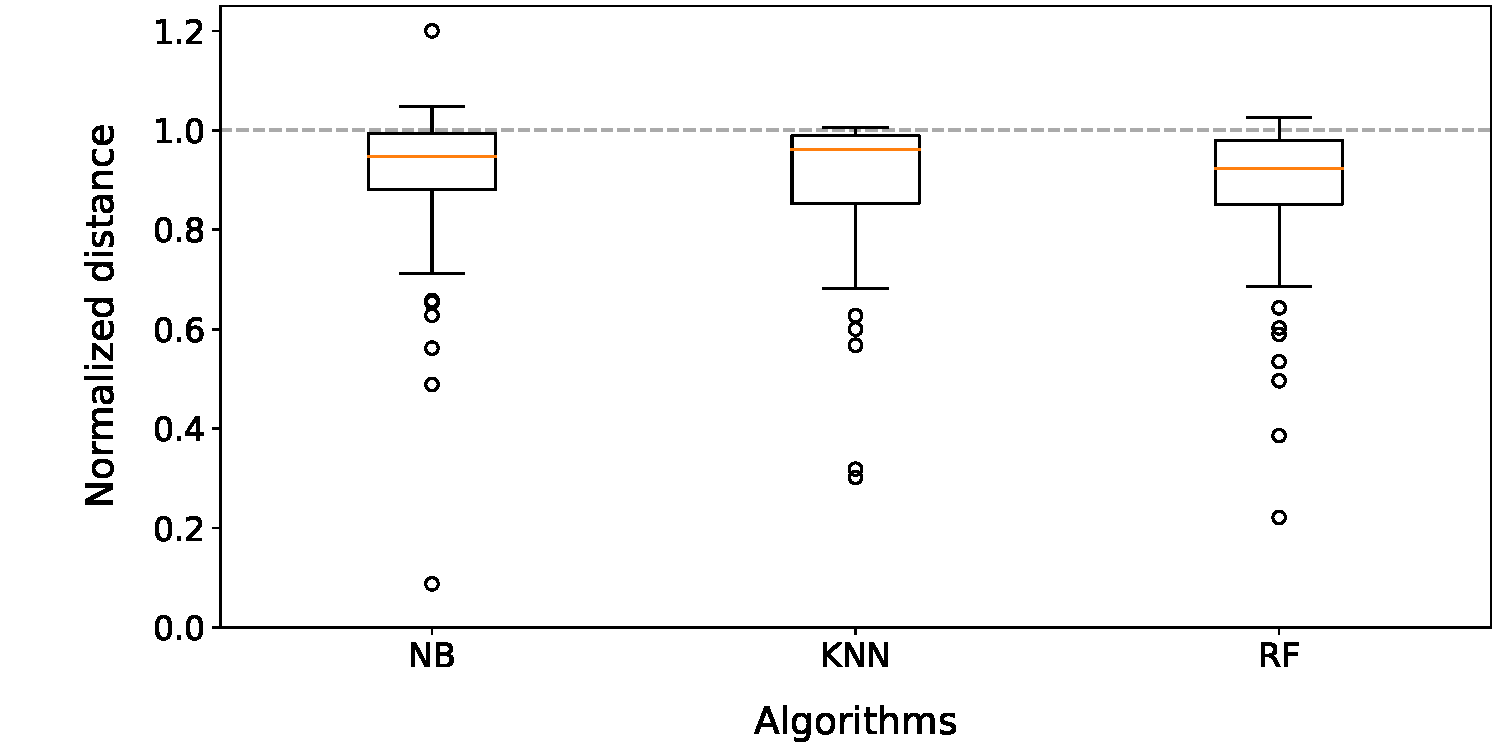
\includegraphics[width=0.7\textwidth]{part-automl/chapter-supervised/img-effective/evaluation2.pdf}
    \caption{Normalized distances between the scores obtained by optimizing our effective prototypes and the ones obtained optimizing the exhaustive set.}
    \label{fig:eval-exhaustive-vs-effective}
\end{figure}

\subsubsection{Complementing hyper-parameter optimization with pre-processing}
\label{ssec:eval-dpso-vs-cash}

\begin{figure*}[!t]
	\centering
	\includegraphics[width=1.0\textwidth]{part-automl/chapter-supervised/img-effective/barplot-10.pdf}
	\caption{The impact of dedicating a portion of the optimization budget to pre-processing compared to using the whole optimization budget for the hyper-parameter optimization.}
	\label{fig:eval-pre-processing-hyper-parameter}
\end{figure*}

We have just shown that our effective pipeline prototypes have similar impact as the exhaustive prototypes. Now we want to compare the impact of effective prototypes against optimizing only the hyper-parameters of the ML algorithm. That is, we want to examine whether dedicating a part of the optimization budget to the pre-processing pipeline impacts more (positively) the results of the analysis, than using the whole budget for the hyper-parameter optimization\footnote{To enable the application of the ML algorithms on all the datasets, whenever required, we apply the necessary transformation (e.g, imputation or encoding).}. 

To this end, for the latter we now dedicate the total optimization budget (i.e., 400 seconds), and for the former, inspired by \cite{Quemy20InfSystems}, we split the budget 50-50 between the pre-processing pipeline optimization and the hyper-parameter optimization (i.e., 200 seconds for the pre-processing, and 200 seconds for the hyper-parameter optimization). The time for the pre-processing is further split among the five different pipeline prototypes (i.e., 40 seconds each).

To compare the results, we calculate the impact using the formulas below, that correspond to the normalized distance from either pre-processing or hyper-parameter optimization to the maximum improvement that can be achieved, regardless of whether pre-processing is applied or not. 

\begin{equation*}
    \text{\textit{pp impact}} = \frac{Acc(d_{e\!f\!f\!ective},a^*) - Acc(d,a)}{max(Acc(d_{e\!f\!f\!ective},a^*),Acc(d,a^*)) - Acc(d,a)}
\end{equation*}

\begin{equation*}
    \text{\textit{hp impact}} = \frac{Acc(d,a^*) - Acc(d,a)}{max(Acc(d_{e\!f\!f\!ective},a^*),Acc(d,a^*)) - Acc(d,a)}
\end{equation*}

where, $Acc(d,a)$ is the baseline accuracy (i.e., predictive accuracy of the algorithm $a$ with default hyper-parameters over the original dataset $d$). $Acc(d_{e\!f\!f\!ective},a^*)$ is the accuracy of the optimized algorithm $a^*$ over the dataset $d_{e\!f\!f\!ective}$ transformed using the optimized instantiation of the effective set of prototypes obtained using our method. Finally,  $Acc(d,a^*)$ is the accuracy of the optimized algorithm $a^*$ (i.e, using the entire budget) over the original dataset $d$.

To obtain relative values that sum to 1, we normalize the impacts dividing them by their sum. For instance, for the pre-processing score we calculate the following:
\begin{equation*}
    \text{\textit{normalized pp impact}} = \frac{\text{\textit{pp impact}}}
    {\text{\textit{pp impact}} + \text{\textit{hp impact}}}
\end{equation*}


We perform the same for the hyper-parameter impact and plot the results obtained for all the algorithms and datasets in Figure~\ref{fig:eval-pre-processing-hyper-parameter}, where each bar represents the results obtained for a single dataset. The different colors represent the impact values of pre-processing and hyper-parameter optimization. 

Observing the bar-charts one can see that (i) dedicating a portion of the budget to pre-processing, brings benefit to the analysis in most of the cases (i.e., $73\%$ of the cases), and (ii) the impact of hyper-parameter optimization, increases with the increase of the number of hyper-parameters of the ML algorithm (e.g., hyper-parameter optimization impacts more RF than NB). Overall, we can conclude that pre-processing is a critical step that once effectively applied may have a high positive impact on the final result of the analysis.


\subsection{Related work}
\label{ssec:relatedwork}
A lot of ongoing research aims at addressing the problem of providing user assistance for the data analytics process.
Specifically, they can be classified into three main categories~\cite{elshawi2019automated}: distributed, cloud-based, and centralized. The first two try to address the problem of Big Data. Thus, clusters of several machines are employed to distribute the workload. On the contrary, this is not a fundamental requirement for centralized solutions. Indeed, the overhead of using a cluster is not worth for relatively small datasets. 
Since our work belongs to the category of centralized solutions, in the following, we provide examples of them.

As already mentioned before, the data analytics process consists of different steps. In general, there is a trend to develop (semi) automatic systems that assist the user in one or many steps altogether. At the beginning, the focus was to provide support exclusively for the learning step (i.e., the CASH problem). Recently however, the direction has shifted towards designing systems that additionally or specifically provide user assistance in the data pre-processing step (i.e., the DPSO problem).

When it comes to data pre-processing, different works have tackled this problem from different perspectives. For instance, there are works that aim to apply pre-processing for the sake of guaranteeing data quality, or enabling data exchange, or even data integration. That is, they consider data pre-processing in isolation or apart from data analysis~\cite{Llunatic13VLDBEnd,BigDansing15SIGMOD,Katara15SIGMOD,Foofah17SIGMOD}. In this, and our related work however, we consider only the works that see pre-processing as an integral part of data analytics and hence apply it for the sake of improving the final result of the analysis.


Finally, there are works that aim at fully automating the data analytics process (i.e., automatically generate data analytics flows), which roughly translates to combining DPSO with CASH, where the border line between the latter two becomes blurry. Nevertheless, we tentatively group the works based on the type of the problem they aim to solve.

\subsubsection{DPSO}

In DPD \cite{Quemy20InfSystems}, the DPSO problem, as we use it in this work, is formally defined. Authors demonstrate the impact of optimizing the pre-processing pipeline, but considering only a single fixed pipeline prototype. %and only a few datasets. 
However, as we have already seen (Section~
\ref{sec:eval-universal-pipeline}), a single fixed prototype cannot perform best for every dataset. Therefore, we build on top of~\cite{Quemy20InfSystems}, and instead of relying on a fixed prototype, we define a method to generate the right pipeline prototypes to be optimized.

In PRESISTANT~\cite{presistant18CSI,presistant18CAISE,presistant19DKE}, we tackled the problem of recommending pre-processing operators to the non-expert data analyst. The goal, and at the same time the challenge was to identify the pre-processing operators, and rank them in advance, based on their potential impact to the final analysis. However, we did not consider pre-processing pipelines, but only single transformations, expecting that the analyst applies the process iteratively. In this work, we consider sets of transformations and thus study the impact of combining transformations into a pipeline. 

In ActiveClean \cite{ActiveClean16PVLDB}, authors define an algorithm that aims at prioritizing the cleaning of records that are more likely to affect the results of the statistical modeling problems, assuming that the latter belong to the class of convex loss models (i.e., linear regression and SVMs). Hence, instead of recommending the transformations to be applied, the system recommends the subset of data which needs to be cleaned at a given point. The type of pre-processing to be applied is left to the user, assuming that the user is an expert. 

In Learn2Clean~\cite{Berti19WWW}, based on a reinforcement learning technique, for a given dataset, and an ML model, an optimal sequence of operators for pre-processing the data is generated,
such that the quality of the ML model is maximized. Here, similarly to~\cite{Quemy20InfSystems}, the pipeline prototype is fixed in advance. Our work is a step further in that we help to choose the right pipeline prototype, instead of fixing it in advance. 

In Alpine Meadow~\cite{Shang19SIGMOD}, authors follow a similar approach to ours in that they define two steps for the pre-processing phase. One, the so called \textit{logical pipeline plan}, which is roughly equivalent to the \textit{pipeline prototypes} defined in this work, and the second the \textit{physical pipeline plan} which translates to \textit{pipelines} used in this work. The physical plan is generated through a combination of Bayesian optimization, meta-learning, and multi-armed bandits. For the logical plans, they rely on rules but without clear evidence on how they are generated. Moreover, it is not clear whether the logical plan is fixed as in~\cite{Quemy20InfSystems} and if some further adjustment from the user is required. 

\subsubsection{CASH} The task in solving the CASH problem is to automatically find an optimized instantiation for the hyper-parameters of the ML algorithm. Most of the works use Bayesian optimization methods to tune and optimize them~\cite{Feurer15AutoSklearn,Thornton13AutoWeka,Olson16Tpot}. Since Bayesian optimization is randomized, meta-learning has been used to find a good seed for the search~\cite{Feurer15AAAI}. Most of these works however, only minimally consider the data pre-processing step.
Auto-WEKA~\cite{Thornton13AutoWeka}, based on the Java machine learning library Weka, is the pioneer of the field.
The authors formalized the problem of algorithm selection and their associated hyper-parameter optimization, and solved it in a combined search space. 
Sequential Model-based Algorithm Configuration (SMAC) is used to explore the large search space.

Autostacker~\cite{chen2018autostacker} combines a hierarchical stacking architecture and an evolutionary algorithm (EA).
Stacking is an ensemble method that involves the concatenation of several classifiers, so that the later layers can learn the mistakes that classifiers in the previous layers make.
Even if it brings some benefits, this approach affects the search space: way larger than that of a single classifier.
In a nutshell, such concatenations are randomly generated and then optimized.
The one that achieves the higher predictive accuracy is chosen.
Rather than Bayesian Optimization, to find suitable hyper-parameters, the authors utilize a basic Evolutionary Algorithm.

OBoe~\cite{yang2019oboe} exploits collaborative filtering for AutoML, choosing models that have performed well on similar datasets.
It collects a large number of datasets and applies different ML algorithms (with different hyper-parameters configurations). 
In this way, a matrix of cross-validated errors is built.
Common approaches typically compute dataset meta-features and use them to predict the error of a particular machine learning model, but OBoe works exactly the other way around.
PCA is applied on such a matrix in order to find latent meta-features.
Given a new dataset, some basic algorithms are applied to infer a feature vector (i.e., the value of the latent meta-features).
Finally, the feature vector is leveraged to estimate the cross-validated error of more complex algorithms.

\subsubsection{DPSO + CASH}
Auto-sklearn~\cite{Feurer15AutoSklearn} is based on the popular Python library scikit-learn.
The authors, inspired by Auto-Weka, address the problem with the Sequential Model-based Algorithm Configuration (SMAC).
Furthermore, they improve the approach by adding a meta-learning phase at the beginning (to warm-start the Bayesian Optimization) and an ensemble technique at the end (to suggests multi-classifiers).
Such a system considers pre-processing transformations to generate end-to-end analytic pipelines. 
Yet, they consider a small set of transformations and also consider a single fixed pipeline prototype. 
Our work in a way is complementary to this, since instead of a priori fixing the prototype, we can construct a potentially optimal one (or a set), and then provide it to the tool for it to be instantiated and further optimized.
TPOT~\cite{Olson16Tpot} is a tree-based pipeline optimization tool using genetic programming while requiring little to no expertise from the user. In TPOT however, they only consider one transformation inside the optimization process (i.e., Feature Engineering).


ML-Plan~\cite{mohr2018ml} uses hierarchical planning, a particular form of AI planning, to propose a solution to both the pre-processing and the modeling phases. 
As in context-free grammars, there are complex tasks (non-terminal symbols) that are derived as long as primitive tasks (terminal symbols) are not obtained.
Typically, standard graph search algorithms (e.g., depth-first search, best-first search, etc.) are employed to solve such problems.
ML-Plan successively creates solutions in a global search instead of changing given solutions in a local search. However, due to the problem constraints, they adopt a randomized best-first search, randomly choosing the solution path.

AutoBazaar~\cite{AutoBazaar} is a Python open-source tool.
Like in ML-Plan~\cite{mohr2018ml}, both pre-processing and modeling phases are covered.
Here the last step of a prototype is the machine learning algorithm.
The approach involves two different steps.
Firstly, a \textit{catalog} proposes a collection of prototypes (with an ML algorithm as last step) based on the task and the dataset itself.
Secondly, the optimization process starts tuning the prototypes until either the time budget is expired or the prototypes are all optimized.
In particular, a \textit{selector} and a \textit{tuner} work in synergy.
The former decides which prototype should be optimized next.
Such a task is treated as a multi-armed bandit problem.
As to the tuner, Bayesian Optimization is chosen.
At the end, the prototype that achieved the higher predictive accuracy is elected.
However, AutoBazaar strictly depends on the catalog.
Such a component memorizes all the possible primitives and supported tasks.
The prototypes are hard-coded for each task.
Thus, it is neither flexible nor maintainable.
If a task is not implemented, the approach cannot suggest a solution.

To summarize, full automation of data analytics has been the ultimate goal of many research works. Yet, such an automation has shown to be computationally expensive, mainly due to the search space involved (i.e., pre-processing and mining operators). Therefore, the usability of these approaches in realistic scenarios is sometimes limited. Our approach of finding a set of effective pipeline prototypes can be seen as complementary to these solutions, since it helps in pruning the large space and guiding the search, hence reducing their cost.

\subsection{Conclusions and future work}
\label{ssec:conclusions}

In this work, we first studied the overall impact of transformations when chained together inside pre-processing prototypes and then delved into examining the impact of instantiating transformations via various operators. As a result, we defined a method that allows to generate effective pre-processing pipelines. That is, pipelines that consist of, (i) compatible pairs of transformations with respect to the framework used,  (ii) meaningful pairs of transformations in terms of general knowledge (best practices), and (iii) promising pairs of transformations that once applied are expected to provide higher overall impact (domain knowledge). 
In addition, via the meta-learning step proposed, we aim to guide the instantiation of transformations in order to facilitate finding better instantiations.

An extensive evaluation on 80 datasets with heterogeneous characteristics, from sample size to feature types, and a set of classification algorithms (i.e., Naive Bayes, Random Forest, K-Nearest Neighbours), showed that our devised pipeline prototypes give promising results. More specifically, we were able to observe that:
\begin{itemize}
    \item [--] The overall impact of optimizing pre-processing is not negligible and it may boost the performance of the overall analytics (e.g., predictive accuracy).
    \item [--] There is no universal pre-processing pipeline prototype that works best for every dataset and algorithm.
    \item [--] With 24 times less time budget, our proposed pipeline prototypes were able to obtain results that were as good as 90\% in the median of the optimal ones found through an exhaustive search.
    \item [--] Dedicating a portion of the time to the pre-processing optimization, instead of dedicating it entirely to hyper-parameter optimization may boost %(have a higher impact on?!) 
    the final result of the analysis. On average, in 73\% of the cases including pre-processing in the optimization, outperformed the results of only optimizing hyper-parameters.
\end{itemize}

The results indicate that pre-processing can boost the performance of the ML algorithm. Hence, it must be considered as an integral part of the data analytics optimization process. 

Finally, previous works have shown the effectiveness of meta-learning for solving the cold start problem~\cite{Feurer15AAAI}, hence as immediate future work, we intend to extend an optimization framework (i.e., HyperOpt) with a complementary meta-learning module that can ease the cold-start problem, facilitating the search for optimal instantiations.

\section{HAMLET}

\begin{figure*}[t]
    \centering
    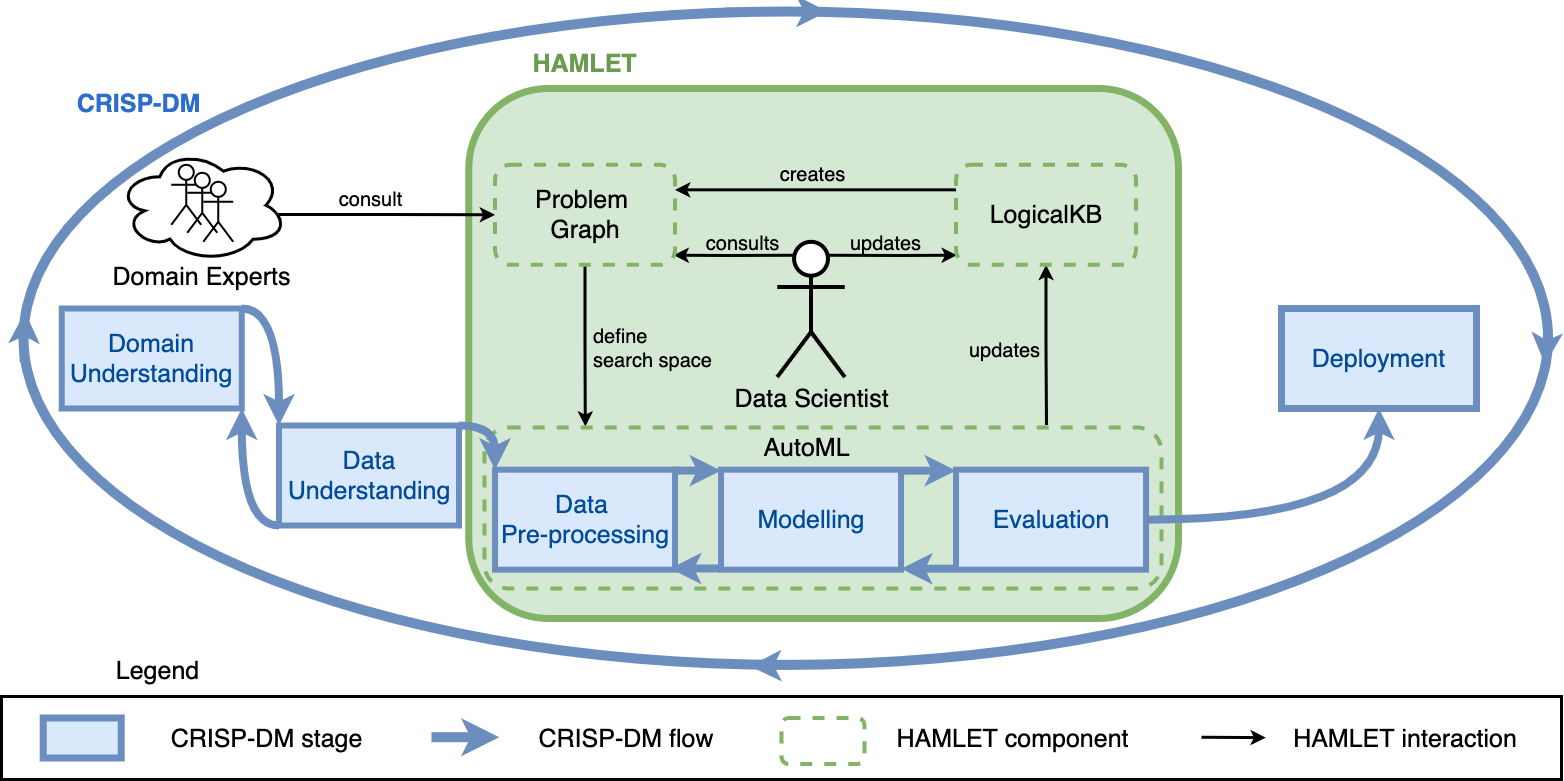
\includegraphics[scale=.3]{part-automl/chapter-supervised/img-hamlet/dymmymodel.png}
    \caption{Integrating HAMLET with the CRISP-DM process model.}
    \label{fig:approach}
\end{figure*}

\subsection{Introduction}\label{intro}
Data platforms, integrated sets of technologies that collectively meet end-to-end data needs, work towards the automation of data management and analysis \cite{DBLP:journals/fgcs/FranciaGGLRS21}.
Machine Learning (ML) plays a key role in such processes (e.g., to devise cost models for querying data over heterogeneous data sources \cite{multi-store} and manage data through lineage \cite{dataplat2}; many applications are well surveyed in \cite{zhou2017ml}).
Data platforms aim at supporting end-to-end data analysis; in this scope, the Cross-Industry Standard Process for Data Mining (CRISP-DM) \cite{wirth2000crisp} is the most acknowledged standard process model---and we will take it as a reference model hencefort.
Given a Machine Learning task to solve, the Data Scientist (DS) collects raw data in arbitrary formats (e.g., from the data lake), builds up knowledge on both the problem and the data, translates such knowledge into \emph{constraints}, designs and trains a model, and finally deploys the solution as a new component integrated into the data platform.
Such a solution consists of a \emph{ML pipeline}: a sequence of \emph{Data Pre-processing transformations} ending with an \emph{ML task}.
The DS instantiates the pipeline among a large set of \emph{algorithms}, which, in turn, can potentially have many \emph{hyperparameters}.
The accuracy of the deployed solution depends on finding both the best algorithms along with their hyperparameters within an exponential search space.

Automated Machine Learning (AutoML) tools assist the DS in finding such an ML pipeline.
They leverage state-of-the-art optimization approaches to smartly explore huge search spaces of solutions.
AutoML has been demonstrated to provide accurate performance, even in a limited time/iteration budget.
When setting up the search space, it is highly important for the DS to inject her knowledge about the problem into constraints that prevent the AutoML tool to retrieve invalid solutions (i.e., the result of those cannot be deemed correct).
However, the support to constraint/knowledge injection is limited and the AutoML tools became that complex to make it difficult for the DS to understand their functioning, hence losing control over the process \cite{XinWLSP21automationml}.

The need for a Human-centered and explainable framework for AutoML is real \cite{gil2019towards, lee2020human, wang2019human} (or even mandatory in recent analytic scenarios where the user is interacting with mixed-reality and smart assistants \cite{DBLP:conf/dolap/FranciaGR19,DBLP:journals/is/FranciaGG22}).
It is crucial for the DS to augment her knowledge by learning new insights (e.g., new constraints) from the retrieved solutions.
Indeed, the DS requires understanding the AutoML process in order to trust the proposed solutions \cite{drozdal2020trust}.
Some works \cite{gil2019towards, lee2020human, wang2019human} prescribe the usage of a Human-centered framework for AutoML, yet they only suggest design requirements.
Alternatively, the authors in \cite{ono2020pipelineprofiler} have proposed a tool that visualizes the best and the worst solutions retrieved by an AutoML tool.
We claim that a Human-centered framework should provide the mechanisms to: (i) help the DS to structure her knowledge about the problem in an effective search space; and (ii) augment the knowledge initially possessed by the DS with the one produced by the AutoML optimization process. 

For this purpose, we introduce HAMLET (Human-centered AutoMl via Logic and argumEnTation; \Cref{fig:approach}), a framework that enhances AutoML with Structured Argumentation to:
structure the constraints and the AutoML solutions in a Logical Knowledge Base (LogicalKB);
parse the LogicalKB into a human- and machine-readable medium called Problem Graph;
devise the AutoML search space from the Problem Graph;
and leverage the Problem Graph to allow both the DS and an AutoML tool to revise the current knowledge.
This paper extends and engineers the vision proposed in \cite{DBLP:conf/edbt/GiovanelliP22} as follows.
\begin{enumerate}[(i)]
    \item We provide an innovative formalization of the AutoML problem, which considers ML pipelines of multiple lengths, Data Pre-processing steps and user-defined constraints.
    \item We design the formal foundation of HAMLET, supporting the injection of constraints to select ML pipelines as well as the resolution of possible arising inconsistencies.
    \item We implement a functioning prototype of HAMLET.
    \item We provide a preliminary empirical evaluation, including the overhead introduced by the argumentation process and the comparison against state-of-the-art algorithms. 
\end{enumerate}

The remainder of the paper is structured as follows. In \Cref{ssec:related}, we introduce the related work and necessary background. Then, we provide the problem formulation in \Cref{ssec:problem} and its implementation in \Cref{ssec:implementation}.
Finally, we provide some preliminary evaluation in \Cref{ssec:test}, and we draw the conclusions and future research directions in \Cref{ssec:conclusion}.

\subsection{Background and Related Work}\label{ssec:related}
HAMLET intersects two research areas, \emph{Automated Machine Learning} and \emph{Argumentation}. 
To the best of our knowledge, no contribution lies in this intersection to provide a Human-centered approach for the optimization of ML pipelines.

\subsubsection{Automated Machine Learning}
AutoML tools lighten the DS in the overwhelming practice of finding the best ML pipeline instance (AutoML contributions mainly refer to supervised tasks).
In the early days, only the optimization of the ML task was addressed (but no pre-preprocessing).
Auto-Weka \cite{kotthoff2019auto} formalized the problem as ``combined algorithm selection and hyperparameter optimization'': various ML algorithms and hyperparameters are tested over a dataset to find the most performing configuration. Such optimization was successfully implemented by leveraging Bayesian optimization \cite{frazier2018tutorial}, a sequential strategy for global optimization: until a limit (budget) of iterations or time is reached, an increasingly accurate model is built on top of the previously explored configurations.

Recently, AutoML is no longer limited to optimizing just the ML task, but it also includes Data Pre-processing \cite{giovanelli2021effective, quemy2019data}.
In doing so, Auto-sklearn \cite{feurer2019auto} fixes the arrangement of the transformations a priori, without considering that the most performing arrangement changes according to the problem and dataset at hand.
However, considering several arrangements translates into larger search spaces that are not easy to explore.

Several improvements have been made to let AutoML tools explore as many configurations as possible.
Multi-fidelity methods \cite{falkner2018bohb} (i.e., the use of several partial estimations to boost the time-consuming evaluation process) have been exploited. 
Meta-learning leverages the previous performance of pipeline instances on a wide range of different datasets to provide several recommendations for the dataset at hand, such as promising pipeline instances (possibly acting as an alternative to Bayesian optimization) and search spaces producing good performance.
Yet, meta-learning per se performs poorly, because it provides coarse-grained recommendations, while it is beneficial in warm-starting Bayesian optimization (i.e., the suggested pipeline instances are visited at the beginning to boost the convergence process).
With respect to HAMLET, meta-learning per se is not expressive enough to be considered as an alternative, but can be leveraged as a support in building the LogicalKB (i.e., learning constraints that resulted effective on many similar datasets).

We believe that the DS has the duty to revise and supervise the suggested solutions as well as the process producing them.
Yet, stacking (more and more) complex mechanisms on top of each other unavoidably led to a less understandable optimization that can be hardly controlled by the DS (especially if without a strong computer science background).

\subsubsection{Towards Human-centered AutoML Approaches}
As of now, the DS role in AutoML is limited to choosing the dataset to analyze, the validation technique (e.g., cross validation, hold out), and the metric to optimize (e.g., accuracy, F1 score).
AutoML researchers aim at making ML accessible to a wider audience;
this has been addressed first by improving automation and now by improving transparency, which also enables human intervention when needed.
Auto-Weka \cite{kotthoff2019auto} and Auto-Sklearn \cite{feurer2019auto} enables non-expert users to build ML models, but the ``black-box'' can be barely open.
Indeed, as advocated in \cite{drozdal2020trust}, DSs require to understand the process to trust the proposed solutions.
This direction, named ``Human-centered AutoML'', is pursued by both researchers and companies.

As to research contributions, we found plenty of visualization wrappers.
In \cite{drozdal2020trust}, the authors raise the need of incorporating transparency into AutoML: after a session interview, they discover that -- out of all their proposed features -- model performance metrics and visualizations are the most important information to DSs when establishing their trust in the proposed solutions.
ATMSeer \cite{wang2019atmseer} provides different multi-granularity visualizations to enable users to monitor the AutoML process and analyze the searched models.
PipelineProfiler \cite{ono2020pipelineprofiler} offers interactive visualizations of the AutoML outputs and enables the reproducibility of the results through a Jupiter notebook.
Other contributions enhance current AutoML techniques towards easier human-interactions by: (i) supporting ethic and fair constraints in Bayesian Optimization through a mathematical encoding \cite{perrone2021fair, yaghini2021human}; (ii) simplifying the usage of AutoML with symbolic annotations \cite{peng2020pyglove} and declarative languages \cite{kraska2013mlbase}; (iii) supporting fast feed-backs from AutoML (i.e., runs that are less time-consuming) by leveraging well-known mechanisms of the DBMS (e.g., lineage optimization) \cite{vartak2015supporting, xin2018accelerating}.
Recently, MILE \cite{lee2020human} has proposed to perform AutoML analysis with an end-to-end framework that reflect a DBMS (i.e., a query language + a lineage optimization).

Companies like Google and IBM are the ones most engaged in boosting the involvement of the human in the loop.
Google Vizer \cite{golovin2017google} and Google Facets\footnote{\url{https://pair-code.github.io/facets/}} are the two main visualization tools.
The former reveals details of the different hyperparameters tried in the optimization \cite{golovin2017google}, and the latter focuses on analyzing the output and recognizes biased AI (e.g., ML models that discriminate on sensible attributes such as gender).
As to IBM, AutoAI \cite{wang2020autoai} and AutoDS \cite{wang2021autods} are the tools developed within the MIT-IBM Watson AI Lab.
Specifically, the former enables non-technical users to define and customize their business goals as constraints. 
The latter assists the DS team throughout the CRISP-DM process (e.g., in data collection and pipeline design \cite{muller2019data, wang2021autods} and in the augmentation of the DS's knowledge about the dataset features \cite{drozdal2020trust}).

Overall, several studies have been made to understand the proper design of a Human-centered AutoML tool.
In \cite{pfisterer2019towards}, the authors overview the main AutoML issues; while in \cite{khuat2022roles} authors suggest improvements towards the Human-centered shift.
In \cite{gil2019towards, XinWLSP21automationml, crisan2021fits}, interviews with DSs are conducted to reveal their perception of AutoML as well as their needs and expectations in the next-generation tools.
The main insight is that the future of data science work will be a collaboration between humans and AI systems, in which both automation and human expertise are indispensable \cite{wang2019human}.
To this end, AutoML should focus on: simplicity, reproducibility, and reliability \cite{XinWLSP21automationml, crisan2021fits}.

While the above-mentioned papers mainly focus on visualization, HAMLET brings the DS in the loop by allowing her to inject knowledge in the form of constraints, optimizing and learning new constraints through AutoML, and managing such constraints and conflicts through Argumentation.

\subsubsection{Logic and Argumentation}\label{logic}
Logic is defined as the abstract study of statements, sentences and deductive arguments \cite{Paulson2018logichistory}.
From its birth, it has been developed and improved widely, now including a variety of formalisms and technologies.

Argumentation is a well-known formal tool for handling conflicting information (e.g., opinions and empirical data).
In Abstract Argumentation \cite{Dung1995abstractArg}, a scenario (e.g., a legal case) can be represented by a directed graph.
Each node represents an argument, and each edge denotes an attack by one argument on another. Each argument is regarded as atomic. There is no internal structure to an argument. Also, there is no specification of what is an argument or an attack. A graph can then be analyzed to determine which arguments are acceptable according to some general criteria (i.e., semantics) \cite{baroniCG11semantics}.

A way to link Abstract Argumentation and logical formalisms has been advanced in the field of Structured Argumentation \cite{BesnardGHMPST14structured}, where we assume a formal logical language for representing knowledge (i.e., a LogicalKB) and for specifying how arguments and conflicts (i.e., attacks) can be derived from that knowledge. 
In the structured approach, the premises and claims of the argument are made explicit, and the relationship between them is formally defined through rules internal to the formalism.
We can build the notion of attack as a binary relation over structured arguments that denotes when one argument is in conflict with another (e.g., contradictory claims or premises).
One of the main frameworks for Structured Argumentation is ASPIC\textsuperscript{+}\cite{Modgil2014aspic+}. 
In this formalism, arguments are built with two kinds of inference rules: strict rules, whose premises guarantee their conclusion, and defeasible rules, whose premises only create a presumption in favor of their conclusion. 
Then conflicts between arguments can arise from both inconsistencies in the LogicalKB and the defeasibility of the reasoning steps in an argument (i.e., a defeasible rule used in reaching a certain conclusion from a set of premises can also be attacked).

Once defined the right logical language for encoding the DS and AutoML knowledge, a Structured Argumentation model (e.g., an ASPIC\textsuperscript{+} instance \cite{arg2p-jlc}) can support HAMLET with the formal machinery to build an Argumentation framework upon the data, while Abstract Argumentation would dispense the evaluation tools.

\subsection{Problem Formulation}\label{ssec:problem}

\Cref{fig:approach} illustrates the overview of HAMLET.
When addressing end-to-end data analysis, a DS usually follows a process model such as CRISP-DM.
The DS starts by collecting raw data in an arbitrary format.
Then, ``Domain Understanding'' is conducted.
The DS works in close cooperation with domain experts and enlists \emph{domain-related constraints} (i.e., intrinsic of the problem).
Follows ``Data Understanding'', devoted to data analysis, and to extract \emph{data-related constraints} (e.g., defined by the data format).
Domain and Data Understanding might be repeated many times until the DS is satisfied by the acquired knowledge.
Once confident, the DS investigates different solutions throughout ``Data Pre-processing'', ``Modelling'', and ``Evaluation''.
Data Pre-processing and Modelling are conducted to effectively build the solution, while Evaluation offers a way to measure its performance.
Such a solution consists of a \emph{ML pipeline}: a sequence of \emph{Data Pre-processing transformations} ending with an \emph{ML task}.
The DS instantiates different pipelines among a large set of algorithms; the performance are affected by both the algorithms and some exposed hyperparameters.
While seeking the best performing and valid solution, the DS should consider the already known constraints -- domain- and data-related -- and the ones she discovers during Data Pre-processing and Modelling, respectively: \emph{transformation-} and \emph{algorithm-related constraints} (e.g., due to the intrinsic semantic of transformations and algorithms at hand).
Finally, the process concludes with the ``Deployment'' of the solution.

HAMLET intersects CRISP-DM, allowing the DS to inject and augment her knowledge while automatizing the exploration towards the solution (i.e., instantiate the best ML pipeline). 
We now dig the foundation of HAMLET by incrementally introducing the concepts necessary to move from AutoML to Logic and Argumentation.
To support the reader, we summarize the main notation in \Cref{tab:symbols}.

\begin{table}[t]
    \centering
    \footnotesize
    \caption{Main symbols used in the formalization.}
    \begin{tabular}{cl}
        \toprule
        \textbf{Symbol} & \textbf{Meaning} \\
        \midrule
        $A$ & Algorithm \\
        $h$ & Algorithm hyperparameter \\
        $S$ & Step \\
        $P$ & Pipeline \\
        $\lambda_*$ & Instance of * \\
        $\Lambda_*$ & Domain of * \\
        $\Lambda$ & Search space \\
        \bottomrule
    \end{tabular}
    \label{tab:symbols}
\end{table}

\subsubsection{AutoML Formalization}
We provide a novel formalization necessary to move from single algorithms to the optimal pipeline.
For the sake of clarity, we refer to a Classification task, but the formalization also holds for supervised ML tasks in general. % regression tasks.

\begin{definition}[Dataset]
A \emph{dataset} $X$ is a matrix where data items (i.e., rows) are characterized by features (i.e., columns).
\end{definition}

\begin{definition}[Algorithm]
An \emph{algorithm} $A$ is a function that transforms an input dataset $X'$ into a new dataset $X''$.
The algorithm exposes a (possibly empty) set $H$ of \emph{hyperparameters}.
Each hyperparameter $h \in H$ has a \emph{domain} $\Lambda_h$.
We call the \emph{algorithm domain} $\Lambda_A$ the Cartesian product of all hyperparameter domains (i.e., $\Lambda_A = \Lambda_{h_1} \times \ldots \times \Lambda_{h_{|H|}}$).
We call \emph{algorithm instance} $\lambda_A \in \Lambda_A$ an algorithm whose hyperparameters have been assigned with values from their respective domains.
\end{definition}

A Classification algorithm returns a vector (i.e., a matrix with a single column) of labels $Y$ out of the input dataset $X'$.

\begin{definition}[Step]
A \emph{step} $S$ is a set of alternative algorithms with the same goal.
The \emph{step domain} is defined as a disjoint union of the algorithm domains $\Lambda_S = \Lambda_{A_1} \cupdot \ldots \cupdot \Lambda_{A_{|S|}}$.
\end{definition}

Where $\cupdot$ combines the domains of the given algorithms, while retaining the original domain membership (i.e., it is possible to refer to the domain of each algorithm included in a step).

We identify two types of steps: Data Pre-preprocessing steps (e.g., Discretization, Normalization) shape the dataset for the last mandatory step, which fulfill the task---Classification in this case.

\begin{example}[Algorithm and step]
Examples of steps are Normalization ($\mathcal{N}$), Discretization ($\mathcal{D}$), and Classification ($\mathcal{C}l$). 
An algorithm for Classification is Decision Tree  ($\mathcal{D}t$) \cite{DBLP:books/wa/BreimanFOS84},
examples of hyperparameters for $\mathcal{D}t$ are its maximum $\textup{depth}$ $(\mathbb{N}^+)$ and the minimum $\textup{samples split}$ $(\mathbb{N}^+)$ required to split a node; hence $\Lambda_{\mathcal{D}t} = \mathbb{N}^+ \times \mathbb{N}^+$.
An example of algorithm instance is $\lambda_{\mathcal{D}t}= \{ \textup{depth}=3,\textup{samples\_split}=10 \}$.
\end{example}

\begin{definition}[Pipeline]
Given a (possibly empty) set of Pre-processing steps $\mathcal{S} = \{S_1,\ldots, S_{|\mathcal{S}|}\}$ and a Classification algorithm $A$ from the Classification step, a \emph{pipeline} $P$ is a sequence that concatenates steps from $\mathcal{S}$ and $A$.
The domain of a pipeline is $\Lambda_P = \Lambda_{S_1} \times \ldots \times \Lambda_{S_{|\mathcal{S}|}} \times \Lambda_A$.
We call \emph{pipeline instance} $\lambda_P$ a sequence of algorithm instances $\lambda_P = \langle \lambda_{A_1}, \ldots, \lambda_{A_{|P|}} \rangle$ such that $\lambda_P \in \Lambda_P$.
\end{definition}

\begin{example}[Pipeline and pipeline instance]
Given the pre-processing steps Normalization ($\mathcal{N}$) and Discretization ($\mathcal{D}$), the possible pipelines for the DecisionTree ($\mathcal{D}t$) are:
\begin{align*}
    P_1 &= \langle \mathcal{D}t \rangle &
    P_2 &= \langle \mathcal{D}, \mathcal{D}t \rangle & 
    P_4 &= \langle \mathcal{D}, \mathcal{N}, \mathcal{D}t \rangle \\
    &&
    P_3 &= \langle \mathcal{N}, \mathcal{D}t \rangle & P_5 &= \langle \mathcal{N}, \mathcal{D}, \mathcal{D}t \rangle
\end{align*}
Given \textup{Binarizer} ($\mathcal{B}$) and  \textup{KBinsDiscretizer} ($\mathcal{K}b$) as algorithms of Discretization ($\mathcal{D}$), and \textup{MinMaxScaler} ($\mathcal{M}m$) and \textup{StandardScaler} ($\mathcal{S}s$) and  as algorithms of Normalization ($\mathcal{N}$), we provide examples of instances of $P_2$ and $P_4$:
\begin{align*}
    \lambda_{P_2} &= \langle \lambda_{\mathcal{B}},~ \lambda_{\mathcal{D}t} \rangle, &\lambda_{P_4} &= \langle \lambda_{\mathcal{K}b},~ \lambda_{\mathcal{M}m},~ \lambda_{\mathcal{D}t} \rangle \\
    \lambda_{\mathcal{B}}&=\{ \textup{thr}=5.5 \}, &\lambda_{\mathcal{K}b}&=\{ \textup{n\_bins}=3, \ldots \}\\
    \lambda_{\mathcal{M}m}&=\{ \varnothing \}, &\lambda_{\mathcal{D}t}&= \{ \textup{depth}=3,\ldots\}
\end{align*}
\Cref{fig:space} depicts the pipeline domain $\Lambda_{P_4}$ and the pipeline instance $\lambda_{P_4}$.
\label{ex:pipelineinstance}
\end{example}

Depending the on the involved algorithms, their order and hyperparameters, the search space -- out of which the best pipeline instance is select -- is defined as follows.
While, its extraction is later discussed in \Cref{spacealgorithm}.

\begin{definition}[Search space]
The \emph{search space} $\Lambda$ is the Cartesian product of the domain of the Classification step and the disjoint union of the all partial permutations of the pre-preprocessing steps domains.
\end{definition}

AutoML optimizes the exploration of such space.
However, it is not only about algorithms and hyperparameters but also about constraints.

\begin{definition}[Constraint]\label{constraints}
A \emph{constraint} $C \subseteq \Lambda$ is a region of search space that is either \emph{mandatory} or \emph{forbidden}.
Given a pipeline instance $\lambda_P \in \Lambda_P \subseteq \Lambda$
\begin{itemize}
    \item a mandatory constraint $C$ is fulfilled if  $\lambda_P \in C$;
    \item a forbidden constraint $C$ is fulfilled if  $\lambda_P \notin C$.
\end{itemize}
\end{definition}

\begin{figure}
    \centering
    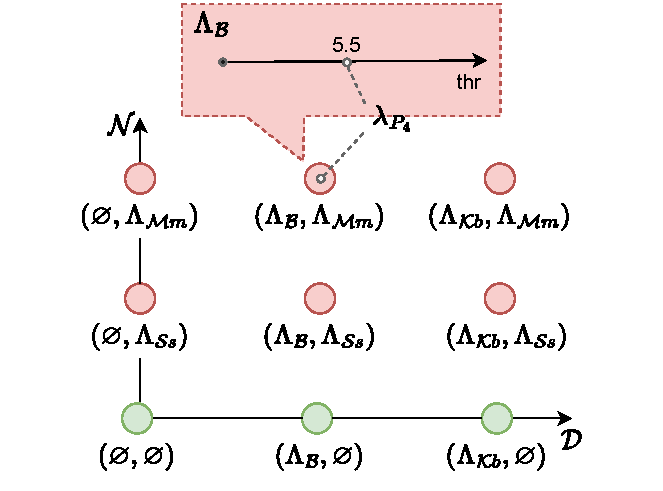
\includegraphics[scale=.75]{part-automl/chapter-supervised/img-hamlet/toy_example_ss.pdf}
    \caption{Examples of the pipeline domain $\Lambda_{P_4}$ and pipeline instance $\lambda_{P_4}$, for the sake of visualization we omit the third dimension representing the domain of the Decision Tree. Green (or red) circles represent valid (or invalid) sub-regions of the search space; Normalization is not allowed in the pipeline. The rectangle represents a zoom in the domain of the Binarizer algorithm.}
    \label{fig:space}
\end{figure}


\begin{example}[Constraint]
Given the Normalization step ($\mathcal{N}$) and Decision Tree ($\mathcal{D}t$) as a Classification algorithm, an example of algorithm-related constraint is ``forbid $\mathcal{N}$ in pipelines with $\mathcal{D}t$''.
This discards all the pipelines containing both Normalization and Decision Tree.
\Cref{fig:space} depicts the effects of the constraint on the pipeline domain $\Lambda_{P_4}$.
\label{ex:constraints}
\end{example}

Considering all the constraint combinations is overwhelming and, additionally, \emph{conflicts} might occur; for instance in the case of ethical \cite{boston-house} and legal fields that easily inject conflicting constraints into the search space.

\begin{definition}[Constrained pipelines optimization]
Given a search space $\Lambda$ and a set of constraints $\mathcal{C}$, finding the best pipeline instance $\hat{\lambda}_P$ is defined as $\hat{\lambda}_P = argmax_{\lambda_P \in \Lambda_P} metric(\lambda_P)$, where $metric(\lambda_P)$ is the function evaluating the goodness of $\lambda_P$ and the explored pipelines fulfill the constraints in $\mathcal{C}$.
\end{definition}

\subsubsection{Argumentation Formalization}

AutoML is not explainable, hence it does not provide the DS with feedbacks that would help her to augment the knowledge about the problem.
It is necessary to represent both (i) the DS knowledge about the problem and (ii) the outcome of the AutoML tool in a uniform human-readable medium.
The former helps to drive the optimization process,
the later augments the knowledge about the problem by learning from the explored configurations of pipeline instances---deriving new constraints that increase the DS awareness.
We leverage Logic as the key element in defining a common structure (i.e., a uniformed human- and machine-readable medium) on which the knowledge of both the DS and the AutoML tool can be combined fruitfully.
In a way, our approach follows the steps of the well known logical based expert systems, of which it is possible to find a great number of successful examples \cite{tan17es}.
Logic provides the tools to cope with one of the distinctive features of the knowledge we want to deal with: inconsistency. Indeed, the ML process is the product of possible attempts, validated or refuted by a consequent evaluation. Hence, the mechanism used to encode the knowledge is required to manage this constant revision process.
This is the role of Argumentation---one of the main approaches for dealing with inconsistent knowledge and defeasible reasoning. 

\begin{definition}[Argumentation Theory]\label{system}
An Argumentation theory is a tuple AS=$\langle L, R \rangle$ with:
\begin{itemize}
    \item $L$ an Argumentation language;
    \item $R$ the set of defeasible rules in the form $r : \phi_0,\ldots, \phi_n \Rightarrow \phi$, where $\phi_0,\ldots, \phi_n,\phi$ are well-formed formulae in the $L$ language and $r$ is the identifier of the rule; we call $\phi_0,\ldots, \phi_n$ the premises of the rule, and $\phi$ its conclusion.
    Rules with no premises are allowed (i.e. $r : \Rightarrow \phi$).
\end{itemize}
\end{definition}

The set of rules $R$ in the theory is used to define how elements from the language are combined together.
In the following two definitions, we specialize $L$ into the language $L_{ML}$ expressing all the basic elements of an AutoML problem and $R$ into a Logical Knowledge Base written in the language $L_{ML}$.

\begin{definition}[AutoML language]
Given an argumentation language $L$, we define the \emph{AutoML language} $L_{ML}$ as $L \cup W$, with $W$ the following set of predicates\footnote{For the sake of conciseness, when writing statements of the AutoML language, the letters $S$ (and $A$) refer to the name of the step (and algorithm)}:
\begin{itemize}
    \item step($S$) with $S \in L$, representing a step $S$ in the pipeline;
    \item algorithm($S$, $A$) with $S, A \in L$, representing an algorithm $A$ for the step $S$;
    \item hyperparameter($A$, $h$, $t$) with $A, h, t \in L$, representing an hyperparameter $h$ for the algorithm $A$ of type $t$ (e.g., numerical, categorical);
    \item domain($A$, $h$, $\Lambda_h$) with $A, h, \Lambda_h \in L$, representing an hyperparameter $h$ for the algorithm $A$ with domain $\Lambda_h$;
    \item pipeline($\langle S_1, \ldots, S_n \rangle$, $A$) with $S_1, \ldots, S_n, A \in L$, representing a pipeline consisting of the sequence of steps $\langle S_1, \ldots, S_n \rangle$ and the Classification algorithm $A$;
    \item mandatory($\langle S_1, \ldots, S_n \rangle$, $Z$) with $S_1, \ldots, S_n, Z \in L$, representing a constraint imposing the steps $\langle S_1, \ldots, S_n \rangle$ on the pipelines with algorithm $A$ ($Z = A$) or on all the Classification pipelines ($Z = \mathcal{C}l$);
    \item forbidden($\langle S_1, \ldots, S_n \rangle$, $Z$) with $S_1, \ldots, S_n, Z \in L$, representing a constraint forbidding the steps $\langle S_1, \ldots, S_n \rangle$ on the pipelines with algorithm $A$ ($Z = A$) or on all the Classification pipelines ($Z = \mathcal{C}l$);
    \item mandatory\_order($\langle S_1, \ldots, S_n \rangle$, $Z$) with $S_1, \ldots, S_n, Z \in L$, representing a constraint imposing the sequence of steps $\langle S_1, \ldots, S_n \rangle$ on the pipelines with algorithm $A$ ($Z = A$) or on all the Classification pipelines ($Z = \mathcal{C}l$).
\end{itemize}
\end{definition}

\begin{definition}[Logical Knowledge Base]
Given the language $L_{ML}$, we call Logical Knowledge Base (LogicalKB) the set of rules for a given AutoML problem.
\end{definition}


In other words, the DS leverages an intuitive logical language (i.e., $L_{ML}$), and enlists the constraints one-by-one (i.e., in the LogicalKB).
In our vision, the LogicalKB consists of (i) a set rules specified by the DS and a (ii) set of common rules that enable the automatic derivation of pipelines and constraints.
Besides, the DS community could create a shared LogicalKB derived from the available literature and similar real-case problems.

\begin{example}[Logical Knowledge Base]\label{ex:kb}
We focus on Discretization ($\mathcal{D}$),  Normalization ($\mathcal{N}$) and Classification ($\mathcal{C}l$) steps, and, for brevity, only define the Classification algorithms: Decision Tree ($\mathcal{D}t$) and K-Nearest Neighbors ($\mathcal{K}nn$).
\begin{lstlisting}[mathescape=true]
# define Discretization step
s1 : $\Rightarrow$ step($\mathcal{D}$).
# define Normalization step
s2 : $\Rightarrow$ step($\mathcal{N}$).
# define Classification step
s3 : $\Rightarrow$ step($\mathcal{C}l$).
# DT is a Classification algorithm
a1 : $\Rightarrow$ algorithm($\mathcal{C}l$, $\mathcal{D}t$).
# Knn is a Classification algorithm
a2 : $\Rightarrow$ algorithm($\mathcal{C}l$, $\mathcal{K}nn$).
# Forbid Normalization when using DT
c1 : $\Rightarrow$ forbidden($\langle\mathcal{N}\rangle$, $\mathcal{D}t$).
\end{lstlisting}
\noindent \texttt{s1}, \texttt{s2}, and \texttt{s3} represent the steps; \texttt{a1} and \texttt{a2} represent the algorithms; finally, \texttt{c1} represent the algorithm-related constraint from \Cref{ex:constraints}, namely ``forbid $\mathcal{N}$ in pipelines with $\mathcal{D}t$''.
\end{example}

\begin{figure*}
    \centering
    \begin{subfigure}[b]{0.3\textwidth}
        \centering
        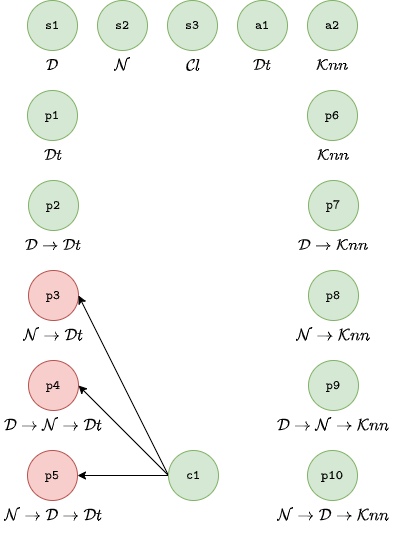
\includegraphics[width=\textwidth]{part-automl/chapter-supervised/img-hamlet/toy_example1.png}
        \caption{}
        \label{fig:running_a}
    \end{subfigure}
    \hfill
    \begin{subfigure}[b]{0.3\textwidth}
        \centering
        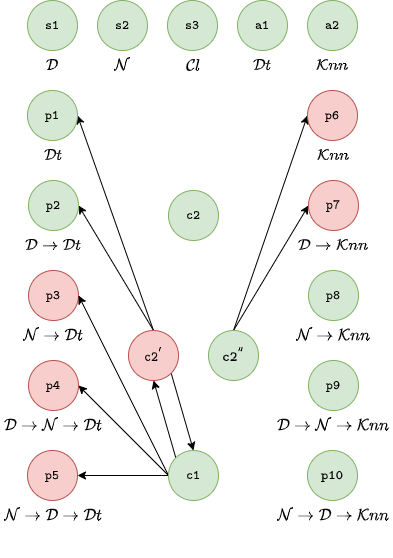
\includegraphics[width=\textwidth]{part-automl/chapter-supervised/img-hamlet/toy_example2.png}
        \caption{}
        \label{fig:running_b}
    \end{subfigure}
    \hfill
    \begin{subfigure}[b]{0.3\textwidth}
        \centering
        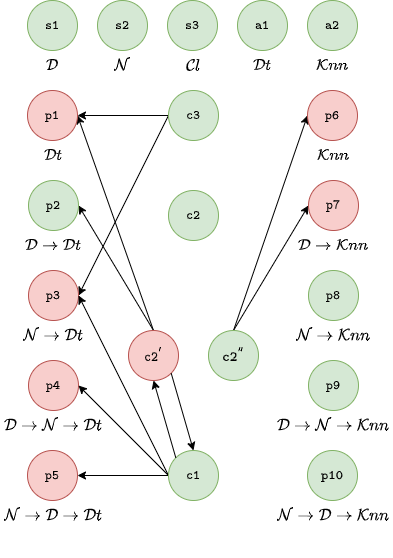
\includegraphics[width=\textwidth]{part-automl/chapter-supervised/img-hamlet/toy_example3.png}
        \caption{}
        \label{fig:running_c}
    \end{subfigure}
    \caption{Examples of Problem Graphs. Green nodes are valid arguments, red ones are refuted. Arrows are attacks.}
    \label{fig:toy_example}
\end{figure*}

When applying constraints, they can be conflicting.
We reify the constraints from \Cref{constraints} through conflict function in the Structured Argumentation domain-

\begin{definition}[AutoML Conflict]\label{conflictauto}
The conflict function $c_{ML}$ is a function from $L_{ML}$ to $2^{L_{ML}}$ that given a statement from $L_{ML}$ returns the set of conflicting statements.
\end{definition}

We support both the AutoML conflicts on ``pipeline vs constraint'' and ``constraint vs constraint''. 
Formally, let us consider two lists of steps $\alpha = \langle \ldots, S_i, S_j, \ldots \rangle$ and $\beta = \langle \ldots, S_y, S_x, \ldots \rangle$.
\begin{itemize}
    \item Pipeline vs constraint: return the constraints conflicting with pipelines.
    \begin{align*}
    c_{ML}&(pipeline(\beta, A)) = \\
        &\{mandatory(\alpha, A)~|~\exists S_i \in \alpha~s.t.~S_i \notin \beta\}~\cup \\
        &\{forbidden(\alpha, A)~|~\forall S_i \in \alpha,~S_i \in \beta \}~\cup\\
        &\{mandatory\_order(\alpha, A)~|~\exists S_i, S_j \in \alpha, S_x, S_y \in \beta, \\&\qquad\qquad\qquad S_i = S_x, S_j = S_y~s.t.~i < j, x > y\}
    \end{align*}
    Intuitively, a pipeline $pipeline(\langle S_i, S_j \rangle, A)$ is conflicting with a $mandatory$ constraint if the pipeline does not contains at least a mandatory step (e.g., the pipeline is conflicting with $mandatory(\langle S_j, S_k \rangle, A)$), with a $forbidden$ constraint if the pipeline contains all the forbidden steps (e.g., the pipeline is conflicting with $forbidden(\langle S_j \rangle, A)$), and with a $mandatory\_order$ constraint if the pipeline contains at least two steps that are not in the mandatory order (e.g., the pipeline is conflicting with $mandatory\_order(\langle S_j, S_i \rangle, A)$).
    \item Constraint vs constraint: return the constraints conflicting with other constraints.
    \begin{align*}
        c_{ML}&(forbidden(\beta, A)) = \{mandatory(\alpha, A)~|~\forall S_j \in \beta, S_j \in \alpha\}\\
        c_{ML}&(mandatory(\beta, A)) = \{forbidden(\alpha, A)~|~\forall S_j \in \alpha, S_j \in \beta\}\\
        c_{ML}&(mandatory\_order(\beta, A)) = \\
        &\{mandatory\_order(\alpha, A)~|~\exists S_i, S_j \in \alpha, S_x, S_y \in \beta, \\&\qquad\qquad\qquad S_i = S_x, S_j = S_y~s.t.~i < j, x > y\}
    \end{align*}
    Intuitively, $mandatory$ and $forbidden$ constraints are in conflict if all the forbidden steps are included in the mandatory constraint (i.e.,  $mandatory(\langle S_i, S_j, S_k \rangle, A))$ and a $forbidden(\langle S_i, S_j \rangle, A))$), this hold symmetrically for $forbidden$ and $mandatory$ constraints. Two $mandatory\_order$ constraints are in conflict if they contain at least two steps in different order (i.e.,  $mandatory\_order(\langle S_i, S_j, S_k \rangle, A))$ and a $mandatory\_order(\langle S_j, S_i \rangle, A))$).
\end{itemize}


\begin{example}[AutoML conflict]
With reference to the LogicalKB in \Cref{ex:kb}, let us consider the set of rules that represent the pipelines related to $\mathcal{D}t$:
\begin{lstlisting}[mathescape=true]
# pipeline ending with a DT
p1 : $\Rightarrow$ pipeline($\mathcal{D}t$).
# Discretization and DT
p2 : $\Rightarrow$ pipeline($\langle\mathcal{D}\rangle$, $\mathcal{D}t$).
# Normalization and DT
p3 : $\Rightarrow$ pipeline($\langle\mathcal{N}\rangle$, $\mathcal{D}t$).
# Discretization, Normalization, and DT
p4 : $\Rightarrow$ pipeline($\langle\mathcal{D}$, $\mathcal{N}\rangle$, $\mathcal{D}t$).
# Normalization, Discretization, and DT
p5 : $\Rightarrow$ pipeline($\langle\mathcal{N}$, $\mathcal{D}\rangle$, $\mathcal{D}t$).
\end{lstlisting}
In this case, \texttt{c1} (i.e., ``forbid $\mathcal{N}$ in pipelines with $\mathcal{D}t$'') is in conflict with the \emph{pipeline} statements \texttt{p3}, \texttt{p4}, and \texttt{p5} since they contain $\mathcal{N}$ and $\mathcal{D}t$.
\label{ex:conflict}
\end{example}

To create a Problem Graph, which is the medium readable by users and machines, we informally (for the sake of conciseness) introduce the key elements from Structured Argumentation; a complete formalization is available in \cite{Modgil2014aspic+}.
Given an Argumentation theory, an \emph{argument} is created for every rule with no premises (e.g., from the rule $r : \Rightarrow c$, we derive an argument with \emph{conclusion} $c$ using $r$).
Then, we recursively apply the other rules in the theory to the newly generated argument (e.g., we can use the argument with conclusion $c$ and the following rule $r1 : c \Rightarrow d$ to conclude an argument for $d$ using $r$ and $r1$).
This is repeated until no new argument can be generated.
In the rest of the paper we will refer to an argument with the set of rules used to generate it (e.g., given $r : \Rightarrow c$ and $r1 : c \Rightarrow d$, we will write $r$ and $r1$ when referring to the rules and $\{r\}$ and $\{r, r1\}$ for -- respectively -- the argument with \emph{conclusion} $c$ using $r$ and the argument with \emph{conclusion} $d$ using $r$ and $r1$).

An \emph{Argumentation framework} is defined using the arguments built from an Argumentation theory and their \emph{attack} relations.
Attacks are inconsistencies between arguments' conclusions and are computed using a conflict function (\Cref{conflictauto}).
For instance, given two arguments concluding respectively $a$ and $b$, and the conflict function $c$ such that $c(a) = \{b\}$, then the argument for $b$ directly attacks the one for $a$ (i.e., $b$ is in conflict with $a$).
The attack is propagated to all the arguments built over the receiver of the attack (e.g., if $a_1$ directly attacks $a_2$, and $a_2$'s conclusion is used to derive $a_3$, then $a_1$ also attacks $a_3$).
Also, we can define a \emph{preference} relation over arguments using a partial ordering over the rules in the Argumentation theory:
it is impossible for an argument to be attacked by the least preferred ones, even if they are in conflict.
In other words, we can explicitly solve inconsistencies in the LogicalKB using priorities.
We exploit the \emph{last-weakest} ordering as in \cite{Modgil2014aspic+}.

Finally, the evaluation of an Argumentation framework is performed through semantics, which determines all the sets of arguments that are consistent (called \emph{extensions}) in an Argumentation framework.
We exploit grounded semantics \cite{Dung1995abstractArg} to produce a \emph{grounded extension}; this semantics is the most skeptical---i.e., it includes only the arguments that are verified by all the possible interpretations. % of the graph.

\begin{definition}[Problem Graph]
We call \emph{Problem Graph} a graph in which nodes are arguments and edges are attacks from the Argumentation framework that is built on the Argumentation theory $\langle L_{ML}, LogicalKB \rangle$ and the conflict function $c_{ML}$.
\end{definition}

The benefits of the Problem Graph are two-fold.
First of all, it can be leveraged by both DSs and domain experts to: understand, summarize and visualize the current knowledge.
Second of all, it is straightforward to convert such a graph of constraints into a space of possible solutions (i.e., exploiting Argumentation semantics, it is easy to obtain all the sets of arguments -- constraints and pipelines -- which hold together).

\begin{example}[Problem Graph]
\Cref{fig:toy_example}a illustrates the Problem Graph extracted from the LogicalKB introduced in \Cref{ex:kb,ex:conflict} and evaluated under grounded semantics.
Arguments are represented as nodes, attacks as arrows and the colors represent the state of the arguments according to the semantics: red for refuted arguments, and green for the ones in the extension.
The arguments are identified through the set of rules used to build them.
In the upper part of the figure, we have a group of undefeated arguments, namely \texttt{\{s1\}}, \texttt{\{s2\}}, \texttt{\{s3\}}, \texttt{\{a1\}}, and \texttt{\{a2\}}, representing the basic knowledge used to setup the AutoML search space (i.e. steps and algorithms).
Then, we have an argument for every pipeline in \Cref{ex:conflict}: from \texttt{\{p1\}} to \texttt{\{p5\}} the pipelines regarding $\mathcal{D}t$, from \texttt{\{p6\}} to \texttt{\{p10\}} the ones regarding $\mathcal{K}nn$.
Finally, we can observe three different attacks: from \texttt{\{c1\}} to \texttt{\{p3\}}, \texttt{\{p4\}}, and \texttt{\{p5\}}, in accordance with the conflicts identified in \Cref{ex:conflict}.
The arguments in the extension give us all the information that we should use during the AutoML optimization process -- i.e. we should discard all the pipelines refuted by the constraint argument ($\{c1\}$), and focus on the remaining part of the search space.
\label{ex:graph}
\end{example}

The use of Argumentation relieves the DS of the burden of manually considering all the effects of the possible constraints.
It is important to notice that, although the increased degree of automation, the Problem Graph allows the DS and domain experts to correct, revise, and supervise the process.
Accordingly, possible inconsistencies -- due to diverging constraints -- can be verified by the DS using her knowledge.

Any change in the LogicalKB translates into a change in the Problem Graph, allowing the DS and domain experts to visualize it and argue about it.
The revision of the Problem Graph is the key element in the process of augmenting the knowledge: the DS and domain experts can consult each other and discuss how the new insights relate to their initial knowledge.
Indeed, thanks to the nature of the Problem Graph, it would be extremely easy to identify new possible conflicts and supporting arguments.
Furthermore, AutoML can update the Problem Graph by extracting constraints from the performed exploration, and transposing them into the LogicalKB.
For instance, the DS may not have considered that the dataset contains missing values.
AutoML helps in identifying the new data-related constraint ``require Imputation ($\mathcal{I}$) in all the pipelines'' and adds it to the LogicalKB ($mandatory(\langle \mathcal{I} \rangle, \mathcal{C}l)$).

The described process is compliant with and augments the CRISP-DM process.
The inferred/learned knowledge is automatically handled throughout iterations, supporting the DS in the whole analysis in a continuous revision of the constraints.
\vspace{2cm}

\subsection{HAMLET}\label{ssec:implementation}

\begin{figure*}[t]
\begin{lstlisting}[mathescape=true]
# given an algorithm, create a pipeline including only such algorithm
hc0 : algorithm($\mathcal{C}l$, A) $\Rightarrow$ pipeline($\langle~\rangle$, A).
# given some steps and an algorithm, create a pipeline including such steps and algorithm
hc1 : step($S_1$),$\ldots$,step($S_n$), algorithm($\mathcal{C}l$, A) $\Rightarrow$ pipeline($\langle S_1, \ldots, S_n \rangle$, A).
# given constraints on the Pre-processing steps required for Classification...
# ... apply this constraints to all Classification algorithms
hc2 : mandatory($\langle S_1, \ldots, S_n \rangle$, $\mathcal{C}l$), algorithm($\mathcal{C}l$, A) $\Rightarrow$ mandatory($\langle S_1, \ldots, S_n \rangle$, A).
hc3 : forbidden($\langle S_1, \ldots, S_n \rangle$, $\mathcal{C}l$), algorithm($\mathcal{C}l$, A) $\Rightarrow$ forbidden($\langle S_1, \ldots, S_n \rangle$, A).
hc4 : mandatory_order($\langle S_1, \ldots, S_n \rangle$, $\mathcal{C}l$), algorithm($\mathcal{C}l$, A) $\Rightarrow$ mandatory_order($\langle S_1, \ldots, S_n \rangle$, A).
\end{lstlisting}
\caption{A subset of rules from the LogicalKB.}
\label{rules-arg2p}
\end{figure*}

HAMLET iterates over three phases (\Cref{fig:approach}): (i) the generation of Problem Graph and search space out of the LogicalKB, (ii) the exploration of the search space in compliance with the specified constraints, and (iii) the augmentation of the LogicalKB through a rule recommendation.

% The framework is available at \url{https://github.com/QueueInc/HAMLET}, and it is composed of two sub-modules. 
% The first, written in Kotlin and running on the JVM, exposes a graphical interface on which the DSs can compile and revise the LogicalKB. 
% The module is also responsible for the generation and evaluation of the Problem Graph; it implements the Structured Argumentation functionalities as specified in \Cref{ssec:problem} using \argtup{} \cite{arg2p-jlc}, an ASPIC\textsuperscript{+}-based Kotlin library.
% The second module, written in Python, is responsible for performing the AutoML optimization and the extraction of the new constraints from the explored space.

% \subsubsection{Generation of Problem Graph and Search Space}
% In \Cref{ssec:problem}, we defined the LogicalKB as the set of rules specified by the DS using her knowledge.
% The LogicalKB also includes a set of hard-encoded rules representing inferences necessary to characterize the AutoML problems.
% These rules are joined to the ones defined by the DS and used to build the Problem Graph (i.e., Argumentation framework).

% A subset of rules is shown in \Cref{rules-arg2p}.
% The first two ($hc0$ and $hc1$) define how to automatically derive a pipeline using algorithms and steps.
% The construction of pipelines can be completely automated and the DS should be dispensed from manually enumerating all the possible pipelines as in \Cref{ex:conflict}.
% In particular, the correct set of rules is built dynamically using the steps and algorithms provided by the DS, then they are used to derive all the arguments for the possible pipelines.
% The last three rules ($hc2, hc3$ and $hc4$) encode constraints -- mandatory, forbidden, mandatory\_order -- on all the available algorithms with a single statement (e.g., $mandatory(\langle \mathcal{D} \rangle, \mathcal{C}l)$): it will be automatically used by the framework to derive the constraints for all the specific algorithms in the theory.

% \begin{example}[Hard-coded rules]
% With reference to \Cref{ex:graph} and \Cref{rules-arg2p}, we add rule \texttt{c2} for a new data-related constraint.
% \begin{lstlisting}[mathescape=true]
% # mandatory Norm. in Class. pipelines
% c2 : $\Rightarrow$ mandatory($\langle\mathcal{N}\rangle$, $\mathcal{C}l$)
% \end{lstlisting}
% From the rule \texttt{c2}, the hard-coded rules generate the two arguments
% \texttt{c2' = \{c2, a1, hc2\}} (i.e., $mandatory(\langle\mathcal{N}\rangle, \mathcal{D}t)$) and \texttt{c2'' = \{c2, a2, hc2\}} (i.e., $mandatory(\langle\mathcal{N}\rangle, \mathcal{K}nn)$) that are specific for the Classification algorithms in the LogicalKB.

% However, \texttt{\{c1\}} (i.e., $forbidden(\langle\mathcal{N}\rangle, \mathcal{D}t)$; is in conflict with \texttt{c2'}.
% Depending on her experience, the DS decides to resolve the conflict by specifying an ordering over the rules in the LogicalKB.
% Assuming that the DS prefers \texttt{c1} to \texttt{hc2},
% the argument \texttt{\{c1\}} is preferred to \texttt{c2'} and the attack from the latter is not considered in the final graph.
% \Cref{fig:toy_example}b shows the updated graph.
% Firstly, we observe the support relation between \texttt{\{c2\}} and the generated constraints \texttt{c2'} and \texttt{c2''}.
% Since \texttt{\{c1\}} has no attackers, it is added to extension.
% Consequently, \texttt{c2'} is refuted and the the pipelines attacked by it are correctly reinstated.
% \label{ex:hard_coded_rules}
% \end{example}

% Given the Problem Graph (we recall that the Problem Graph contains \emph{all} the generated pipelines -- including their partial permutations), the search space can be extracted as in \Cref{spacealgorithm}. 
% We iterate over all the generated pipelines in the Problem Graph and we recursively build their domain: the pipeline domain is the Cartesian product of the step domains, the step domain is the disjoint union of the algorithm domains (we leverage the disjoint union since each algorithm can be picked as an alternative to the others), the algorithm domain is the Cartesian product of its hyperparameters; the domain of a hyperparameter is given by definition.
% Finally, the search space is the disjoint union of all the alternative pipeline domains.

% Noticeably, while the search space could be constrained during its construction (e.g., by simply adding an ``if'' condition to check the validity of each pipeline at \Cref{spacealgorithm} line 10), current AutoML frameworks leverage optimization techniques that do not allow the explicit exclusion of regions from the search space.
% As a consequence, we need to produce the entire search space first.

% \begin{algorithm}[t]
% \caption{Search Space from the Problem Graph}
% \label{spacealgorithm}
% \footnotesize
% \begin{algorithmic}[1]
% \Require{PG(N, E): Nodes and Edges of a Problem Graph}
% \Ensure{$\Lambda$: Search Space}
%     \item[]
%     \Procedure{GetDomain}{$A$}
%         \State $\Lambda_A \leftarrow \varnothing$
%         \ForEach{$h \in A$} \Comment{For each hyperparameter in the algorithm...}
%             \State $\Lambda_A \leftarrow \Lambda_A \times \Lambda_h$ 
%             \Comment{Compute Cartesian product of hyperpar. domains}
%         \EndFor
%         \State \Return $\Lambda_A$ \Comment{Return the algorithm domain}
%     \EndProcedure
%     \item[]
%     \State $\Lambda \leftarrow \varnothing$ \Comment{Initialize the search space}
%     \ForEach{$pipeline(\alpha, A) \in N$} \Comment{For each argument that is a pipeline with $\alpha$ steps and alg. $A$...}
%         \State $ \Lambda_{P} \leftarrow \textup{GetDomain(A)}$ \Comment{Init. pipeline domain with algorithm domain}
%         \ForEach{$S \in \alpha$}  \Comment{For each step in the pipeline...}
%             \State $\Lambda_{S}  \leftarrow \varnothing$ \Comment{Init. the step domain}
%             \ForEach{$A \in S$}  \Comment{For each algorithm in the step...}
%                 \State $\Lambda_{S} \leftarrow \Lambda_{S} \cupdot \textup{GetDomain(A)}$ \Comment{Add alg. to step domain}
%             \EndFor
%             \State $\Lambda_P \leftarrow \Lambda_P \times \Lambda_S$ \Comment{Add step domain to pipeline domain}
%         \EndFor
%         \State $\Lambda \leftarrow \Lambda \cupdot \Lambda_P$ \Comment{Add pipeline domain to the search space}
%     \EndFor
%     \State \Return $\Lambda$ \Comment{Return the search space}
% \end{algorithmic}
% \end{algorithm}

% \subsubsection{Exploration of a Constrained Search Space}\label{subsec:constrained_automl}

% The Problem Graph is not only used to build the entire search space but it is also evaluated to understand which pipelines are invalid and which constraints are valid.
% Hence -- through the Problem Graph -- we enhance AutoML exploration by combining the following techniques.
% \begin{itemize}
%     \item[(i)] Invalid pipelines are used to discourage the exploration of such a portion of the search space (we recall that a pipeline has a domain -- a region of the search space -- in which several pipeline instances are parametrized).
%     First, we sample such regions of the search space, then we enforce a knowledge injection mechanism through warm-starting (i.e., the process of providing previous evaluations that help the model to converge faster).
%     For instance, with reference to \Cref{ex:hard_coded_rules}, we sample some pipeline instances from the pipelines that have been discarded (from \texttt{\{p3\}} to \texttt{\{p7\}});
%     then, we label such samples as invalid and provide them to the AutoML tool, helping the optimization algorithm to focus only on the valid portions of the space.
%     \item[(ii)] Valid constraints -- expressed as conjunctions of Boolean clauses -- are used to discard the invalid pipeline instances that still are encountered by the AutoML tool.
%     Indeed, since the sampling from (i) is non-exhaustive, it can happen that small portions of invalid regions could still be explored.
% \end{itemize}

% Our AutoML implementation is based on FLAML \cite{wang2021flaml}, which mixes Bayesian Optimization with CFO (Frugal Optimization for Cost-related Hyperparameters).
% In a standard Bayesian process, an increasingly accurate model is built on top of the previously explored pipeline instances to suggest the most promising ones among the remaining.
% The pipeline instances keep being explored, updating the model, until a budget in terms of either iterations or time is reached.
% With CFO, there is also an estimation of the evaluation time to consider the frugality of the suggested pipeline instances -- hence favoring the ones requiring a smaller amount of time.
% Throughout the exploration, different solutions are tested, which contribute to augmenting the global knowledge about the problem.

% \subsubsection{Knowledge Augmentation through Rule Recommendation}

% New constraints are automatically mined out of the pipeline instances explored by AutoML and \emph{recommended} in our logical language as rules.
% Then, the DS decides which rules are accepted and added to the LogicalKB.


% At this stage, we leverage frequent pattern mining techniques to learn constraints in an unsupervised manner.
% Frequent pattern mining is the task of finding the most frequent and relevant patterns in large datasets (e.g., finding the products frequently bought together in the domain of market basket analysis); depending on the constraint type, we look for (sub)sets \cite{srikant1995mining} or (sub)sequences \cite{srikant1996mining} frequently recurring among the explored pipelines.
% Since a pipeline instance is a sequence of algorithms, the set of the explored pipeline instances can be directly mapped into a transactional dataset \cite{srikant1995mining} where each pipeline instance is a transaction and each step -- inferred from the algorithm -- is an item.

% We recommend the same constraints we support at the Argumentation level (i.e., $mandatory$, $forbidden$, $mandatory\_order$) so that AutoML can be as expressive as the DS.
% For mandatory and forbidden constraints we look for (sub)sets \cite{srikant1995mining} frequently recurring among the explored pipelines.
% Specifically, we split the explored pipeline instances by the applied Classification algorithm, set a minimum frequency (i.e., support) threshold to 50\% (i.e., to be retrieved, a set/sequence must occur at least in 50\% of the explored instances), and extract frequent maximal\footnote{Maximal itemsets are patterns that are not contained in any other.
% For instance, given two frequent patterns, $\{a, b, c\}$ and $\{a, b\}$, the former is maximal while the latter is not.
% }
% itemsets.
% The recommendation depends on the constraint.
% \begin{itemize}
%     \item $mandatory$: we consider only the patterns with good performance (i.e., $0.7 \leq metric \leq 1.0$); 
%     \item $forbidden$: we consider only the patterns with bad performance (i.e., $0.0 \leq metric \leq 0.3$);
%     \item $mandatory\_order$: the same considerations of the mandatory constraints stand, except that we look for (sub)sequences \cite{srikant1996mining} of length 2 to discover ordering dependencies in pairs of steps as in \cite{giovanelli2021data}.   
% \end{itemize}
% We leveraged well-known implementations \cite{raschkas_2018_mlxtend} and \cite{seq2pat2022} for itemsets and sequences mining, respectively.
% Finally, we return to the DS only the top-10 rules sorted by descending support; we allow the DS to explore all the rules on-demand.

% The thresholds act as filters on the extracted rules since we cannot burden the user with the investigation of hundreds of recommendations. 
% As to the intervals, our rationale is simple: we only want to recommend as mandatory (order) the rules that achieved ``good performance'' and as forbidden the rules that achieved ``bad performance''.
% Since we handle classification pipelines that mainly refer to (balanced) accuracy/F1 score/recall, we mapped ``good'' in the interval $[0.7, 1.0]$ and ``bad'' in the interval $[0, 0.3]$. For the frequent pattern extraction, we consider only the pipeline instances falling in these intervals.
% As to the support, 50\% ensures that the pattern recurs on many of the explored instances and empirically showed to be a good threshold to have good efficiency in the extraction of frequent patterns.

% \begin{example}[Rules Recommendation]
% With reference to the Problem Graph in \Cref{ex:hard_coded_rules},
% the AutoML results are filtered according to the chosen metric, the algorithm \cite{raschkas_2018_mlxtend} is applied, and let us assume that the rule \texttt{c3} is recommended:
% \begin{lstlisting}[mathescape=true]
% c3 : $\Rightarrow$ mandatory($\langle\mathcal{D}\rangle$, $\mathcal{D}t$).
% \end{lstlisting}
% The constraints specifies ``mandatory $\mathcal{D}$ in pipelines with $\mathcal{D}t$''.
% As a matter of fact, it is well known that Discretization improves the performance of tree-based algorithms giving to them the ability to apply multiple split in the decision nodes.
% \Cref{fig:toy_example}c shows the effect of the applied constraint: a new portion of the search space is excluded from the extension ($\{p1\}$).
% \end{example}


% \subsection{Experimental Evaluation}\label{ssec:test}

% The performance of HAMLET depends on (i) the rules encoded in the LogicalKB and (ii) the rules recommended after each run.
% To test both the effectiveness and efficiency of our approach, we define three experimental settings.
% \begin{itemize}
%     \item PKB (Preliminary Knowledge Base), HAMLET starts with a preliminary LogicalKB constraining the search space from the first iteration, and no rule mining is applied.
%     %, but the rules that are suggested throughout the iterations are not applied.
%     The preliminary LogicalKB consists of the rules discovered in \cite{giovanelli2021data} and some well-known from the literature (e.g., suggested by scikit-learn\footnote{\url{https://scikit-learn.org/stable/auto_examples/preprocessing/plot_discretization.html}}).
%     The complete knowledge base can be found in the Github repository.
%     \item IKA (Iterative Knowledge Augmentation), HAMLET starts with an empty LogicalKB, and all the rules recommended after each run are applied to extend the LogicalKB.
%     \item PKB+IKA, HAMLET starts with a preliminary LogicalKB, and the rules recommended after each run are applied to extend the LogicalKB.
% \end{itemize}
% HAMLET run 4 times in every setting -- intuitively, four runs of knowledge augmentation -- the budget assigned to each run is 125 pipeline instances in 900 seconds (15 minutes).
% We also test against a baseline: we let AutoML explore 500 pipeline instances ($= 125 \cdot 4$) in a single run with a time budget of 3600 seconds ($= 900 \cdot 4$; 1 hour).

% For such an evaluation, we derive a search space out of 6 steps, 5 Data Pre-processing steps (Imputation, Normalization, Discretization, Feature Engineering, and Rebalancing) followed by the final Classification task.
% Since the tests are run on datasets from OpenML \cite{OpenML2013} -- a well-known repository for data acquisition and benchmarking -- and it provides already-encoded datasets, we do not consider the encoding step. 
% Except for that, we included all the Data Pre-processing steps and algorithms available in the scikit-learn \cite{scikit-learn} Python library (plus imbalance-learn \cite{JMLR:v18:16-365} for Rebalancing transformations).
% The leveraged steps, algorithms per step, and hyperparameters per algorithm are reported in \Cref{tab:search_space}.

% \begin{table}[t]
%     \footnotesize
%     \caption{Algorithms and number of hyperparameters for each of the steps in HAMLET. Algorithm names and hyperparameters are imported from the scikit-learn Python library.}
%     \centering
%     \begin{tabular}{llc}
%         \toprule
%         \textbf{Step} & \textbf{Algorithm} & \textbf{\#Hyperparameters}  \\\midrule
%         Imputation        & SimpleImputer & 1 \\
%                           & IterativeImputer & 2 \\
%         Normalization     & StandardScaler & 2 \\
%                           & MinMaxScaler & 0 \\
%                           & RobustScaler & 2 \\
%                           & PowerTransformer & 0 \\
%         Discretization    & Binarizer & 1 \\
%                           & KBinsDiscretizer & 3 \\
%         Feature Eng.      & SelectKBest & 1 \\
%                           & PCA & 1 \\
%         Rebalancing       & NearMiss & 1 \\
%                           & SMOTE & 1 \\
%         Classification    & DecisionTreeClassifier & 7 \\
%                           & KNeighborsClassifier & 3 \\
%                           & RandomForestClassifier & 7 \\
%                           & AdaBoostClassifier & 2 \\
%                           & MLPClassifier & 6 \\ \bottomrule
%     \end{tabular}
%     \label{tab:search_space}
% \end{table}

% The OpenML-CC18 suite is a well-known collection of 72 datasets for benchmarking.
% Given the time-consuming computation of each dataset (8 hours per dataset = 2 hours for the baseline + 6 hours for HAMLET in the three settings) -- in this preliminary evaluation -- we select a representative subset of datasets according to three meta-features provided by OpenML: number of instances, number of features, and number of classes.
% For each of the considered meta-features, we search for datasets with either high or low values, and we select the representatives that maximize the overall dataset diversification.
% \Cref{tab:datasets} illustrates the 6 datasets that have been identified; note that some combinations of meta-features have no representative dataset in the suite.
% Among these, we do not report the results for the dataset mnist\_784 since the number of explored pipeline instances is insufficient to validate the result (i.e., due to the time necessary to run a single pipeline instance, only 50 instances were explored out of 1000).

% \begin{table}[t]
%     \caption{Dataset descriptions.}
%     \footnotesize
%     \label{tab:meta_features}
%     \begin{threeparttable}
%     \centering
%         \begin{tabular}{ll|ll|ll|ll}
%             \toprule
%              \textbf{OpenMLID} \tnote{a} & \textbf{Dataset} & \multicolumn{2}{c}{\textbf{Instances}} & \multicolumn{2}{c}{\textbf{Features}} & \multicolumn{2}{c}{\textbf{Classes}}  \\ \midrule
%              40983 & wilt & 4839 & \footnotesize{\texttt{L}} & 6 & \footnotesize{\texttt{L}} & 2 & \footnotesize{\texttt{L}}\\
%              40499 & texture & 5500& \footnotesize{\texttt{L}} & 41& \footnotesize{\texttt{L}} & 11& \footnotesize{\texttt{H}}\\
%              1485 & madelon & 2600 & \footnotesize{\texttt{L}} & 501 & \footnotesize{\texttt{H}} & 2 & \footnotesize{\texttt{L}}\\
%              1478 & har & 10229 & \footnotesize{\texttt{L}} & 562& \footnotesize{\texttt{H}} & 6& \footnotesize{\texttt{H}}\\
%              1590 & adult & 48842& \footnotesize{\texttt{H}} & 9& \footnotesize{\texttt{L}} & 2& \footnotesize{\texttt{L}}\\
%              -- & -- & -- & \footnotesize{\texttt{H}} & -- & \footnotesize{\texttt{L}} & -- & \footnotesize{\texttt{H}}\\%[-1.5ex]\hline\noalign{\vspace{\dimexpr 2.ex-\doublerulesep}}
%              -- & -- & -- & \footnotesize{\texttt{H}} & -- & \footnotesize{\texttt{H}} & -- & \footnotesize{\texttt{L}}\\%[-1.5ex]\hline\noalign{\vspace{\dimexpr 2.ex-\doublerulesep}}
%              554 & mnist\_784 & 70000& \footnotesize{\texttt{H}} & 785& \footnotesize{\texttt{H}} & 10& \footnotesize{\texttt{H}}\\%[-1.5ex]\hline\noalign{\vspace{\dimexpr 2.ex-\doublerulesep}}
%              \bottomrule
%         \end{tabular}
%         \label{tab:datasets}
%         \begin{tablenotes}
%             \item[--] {\scriptsize Not Applicable}
%             \item[\texttt{H}] {\scriptsize The value $v$ is high for the meta-feature $F$ if $ v \geq \frac{1}{|F|}\sum_{f \in F} f$}
%             \item[\texttt{L}] {\scriptsize The value $v$ is low for the meta-feature $F$ if $v < \frac{1}{|F|}\sum_{f \in F} f$}
%             \item[a] {\scriptsize Datasets are available at \url{https://www.openml.org/d/<OpenMLID>}}
%         \end{tablenotes}
%     \end{threeparttable}
% \end{table}

% \subsection{Effectiveness}
% \begin{figure}[t]
%     \centering
%     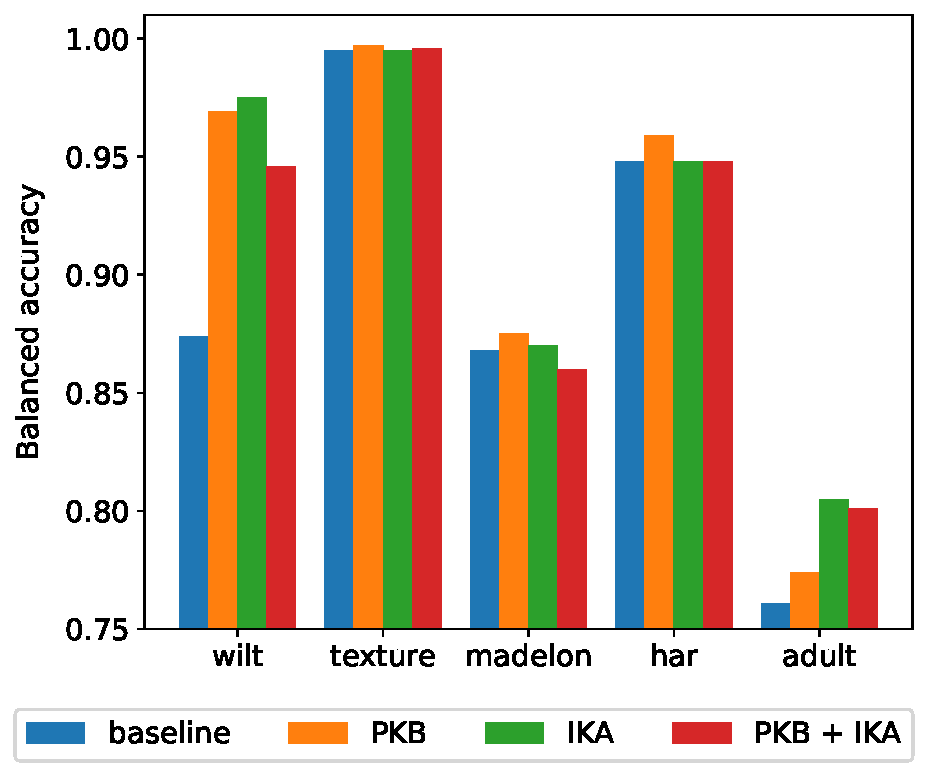
\includegraphics[scale=.45]{part-automl/chapter-supervised/img-hamlet/accuracy.pdf}
%     \caption{Results assessing the effectiveness of HAMLET w.r.t. the baseline.}
%     \label{fig:effectiveness}
% \end{figure}

% \begin{figure*}[h!]
%     \centering
%     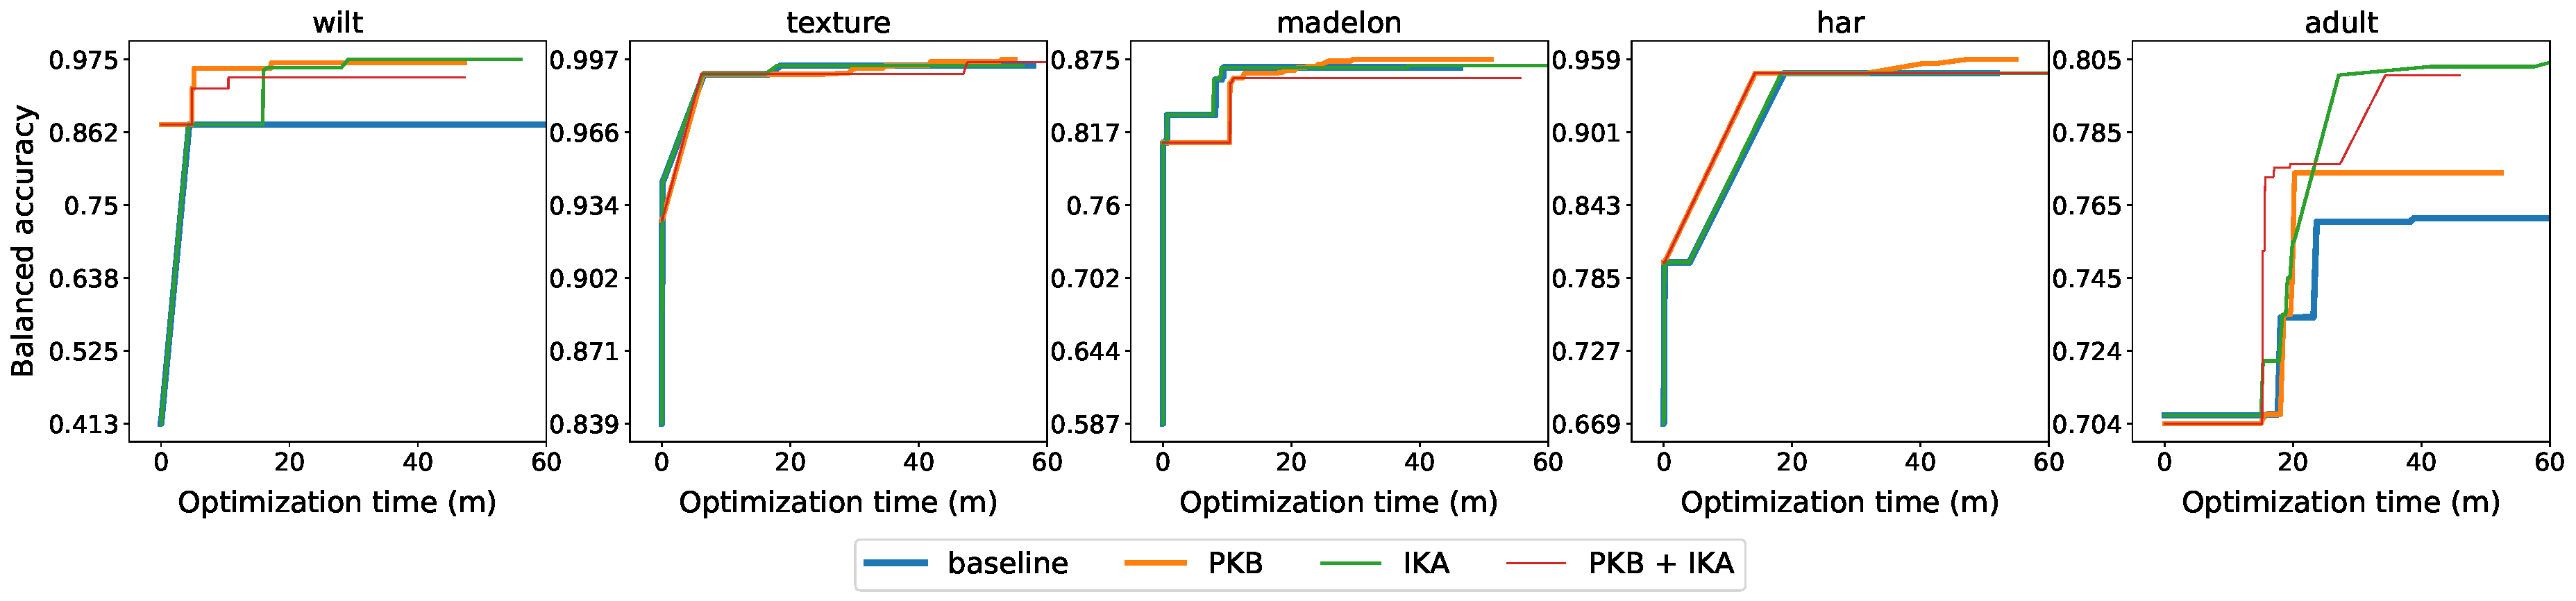
\includegraphics[scale=.3]{part-automl/chapter-supervised/img-hamlet/accuracy_time.pdf}
%     \caption{Results assessing the performance of HAMLET through the optimization time.}
%     \label{fig:efficiency}
%     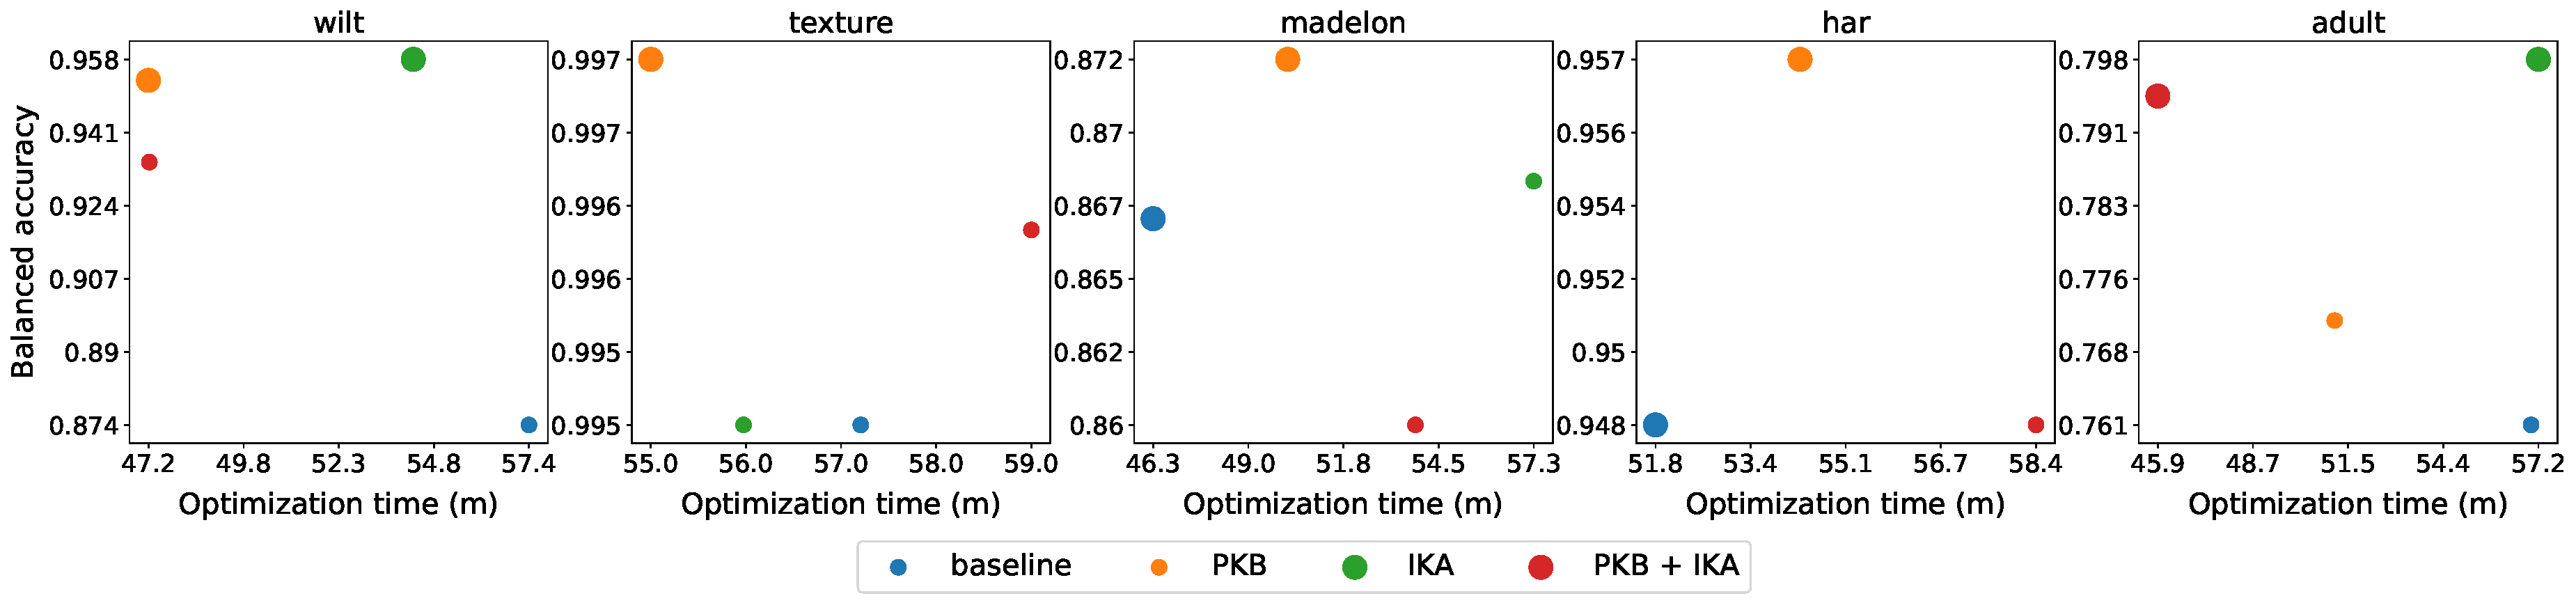
\includegraphics[scale=.3]{part-automl/chapter-supervised/img-hamlet/skyline.pdf}
%     \caption{Comparison of the best pipeline instances characterized by optimization time and (balanced) accuracy, bigger circles represent settings that dominate the others.}
%     \label{fig:effskyline}
% \end{figure*}

% We employ balanced accuracy as the quality metric.
% For instance, in case of (two) binary classes, such a score is
% $$
% \texttt{Balanced accuracy} = \frac{1}{2}\left( \frac{TP}{TP + FN} + \frac{TN}{TN + FP}\right )
% $$
% where $TP$ and $TN$ stand respectively for True Positive and True Negative (i.e., number of instances that have been correctly assigned to the positive and negative classes), and $FP$ and $FN$ stand respectively for False Positive and False Negative (i.e., number of instances that have been mistakenly assigned to the positive and negative classes). The formulation generalized to more than 2 classes can be found at \cite{DBLP:conf/icpr/BrodersenOSB10}.
% The score avoids inflated performance estimations on imbalanced datasets.
% For balanced datasets, the score is equal to the conventional accuracy (i.e., the number of correct predictions divided by the total number of predictions), otherwise it drops to $\frac{1}{\#classes}$.

% \Cref{fig:effectiveness} illustrates the performance achieved by the baseline and the three settings of HAMLET.
% HAMLET is clearly beneficial since in all datasets the framework overcomes the baseline.
% The preliminary results highlight that both the LogicalKB and rule recommendation play important roles:
% \begin{itemize}
%     \item When we warm-start the exploration with a non-empty LogicalKB (PKB), in all datasets HAMLET overcomes the baseline.
%     \item When we only leverage rule recommendation (IKA)}, we achieve results that are better than or equivalent to PKB, indeed we are injecting in the LogicalKB new rules that are tailored to the dataset.
%     \item The synergy of PKB+IKA performs better than PKB in adult, worse in wilt, and the two are comparable in the other datasets.
%     On the one hand, the PKB act as a warm start mechanism that speeds up the optimization; on the other hand, if not aligned with the recommended rules, it can mitigate the benefits of IKA.
%     This proves to be a promising direction that further requires investigation since merging the words will require further studies.
%     Indeed, it is worth noting that the recommended rules can be overlapping with the ones in the LogicalKB, highlighting the need to improve the recommendation process by also considering the rules that are already present in the LogicalKB.
% \end{itemize}

% In PKB+IKA, IKA can introduce rules that contradict the ones in the LogicalKB of PKB; for instance when the PKB contains rules that are not ``representative'' of the dataset/algorithms in use. We believe that this is an added value of HAMLET since ``incomplete'' (or even wrong) LogicalKBs can be corrected/refined by a data-driven approach. Finally, PKB+IKA and IKA are likely to produce different rules, since in PKB+IKA the LogicalKB biases the exploration of the search space from the beginning (acting as a warm start mechanism).


% \subsection{Efficiency}


% \Cref{fig:efficiency} shows how settings converge to the optimal pipeline instance.
% Noticeably, PKB and PKB+IKA start with higher accuracy than IKA and the baseline in four datasets out of five, proving how the preliminary LogicalKB warm starts the exploration.
% However, time and \#iterations alone are not fair metrics for comparison; for instance, an optimization strategy could privilege simple algorithms taking small amounts of computational time but producing worse results than ``more complex'' algorithms.
% In the direction of multi-objective optimization (exploration time should be minimized while accuracy should be maximized), \Cref{fig:effskyline} depicts which settings dominate the others using the Skyline operator \cite{borzsony2001skyline}.
% A setting dominates another one if it is as good or better in all dimensions (time and accuracy) and better in at least one dimension (time or accuracy).
% PKB dominates in 80\% of the datasets, IKA in 40\%, PKB+IKA in 20\%, and the baseline in 40\%.
% Noticeably, the baseline is selected as dominating only in madelon and har datasets due to the fact that converges faster than HAMLET (although it converges to a pipeline instance with lower accuracy).


% \begin{figure}[t]
%     \centering
%     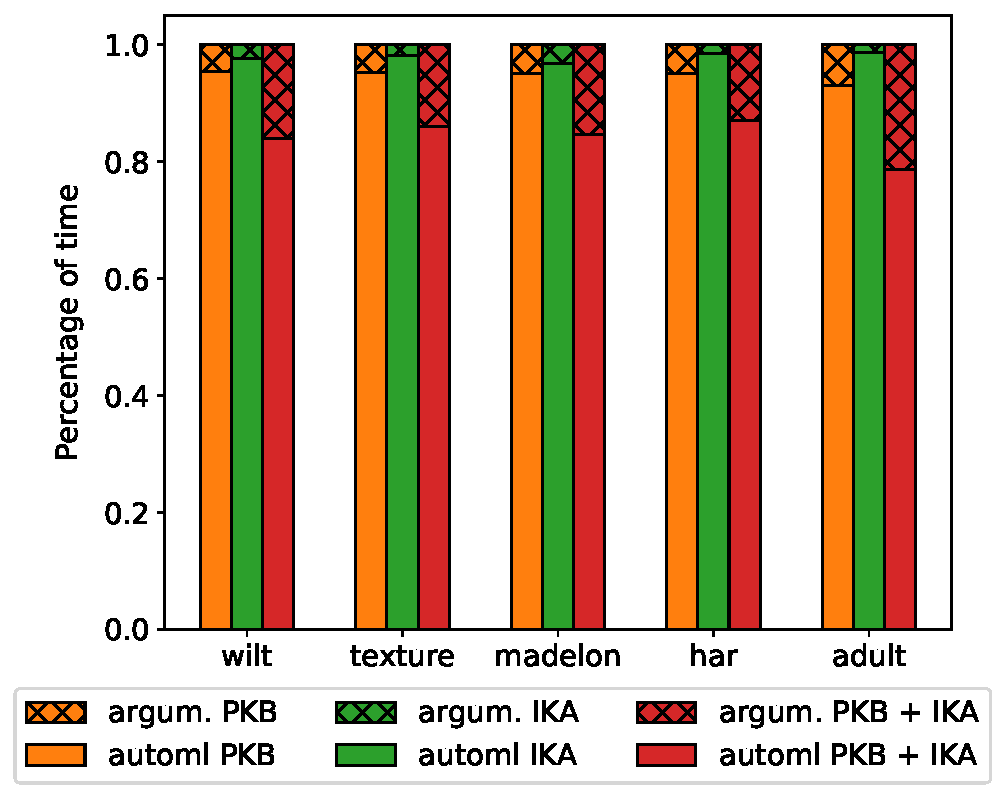
\includegraphics[scale=.43]{part-automl/chapter-supervised/img-hamlet/time.pdf}
%     \caption{Computational time of the argumentation and AutoML processes.}
%     \label{fig:effoverhead}
% \end{figure}


% Finally, \Cref{fig:effoverhead} depicts the overhead introduced by the argumentation framework in HAMLET that, at maximum, is 20\% of the computational time in the adult dataset.
% This proves that the argumentation time is marginal with respect to the duration of the optimization process.
% As expected, PKB+IKA shows the highest overhead since the number of rules to manage is the highest.



% \subsection{Comparison}

% \begin{figure}[t]
%     \centering
%     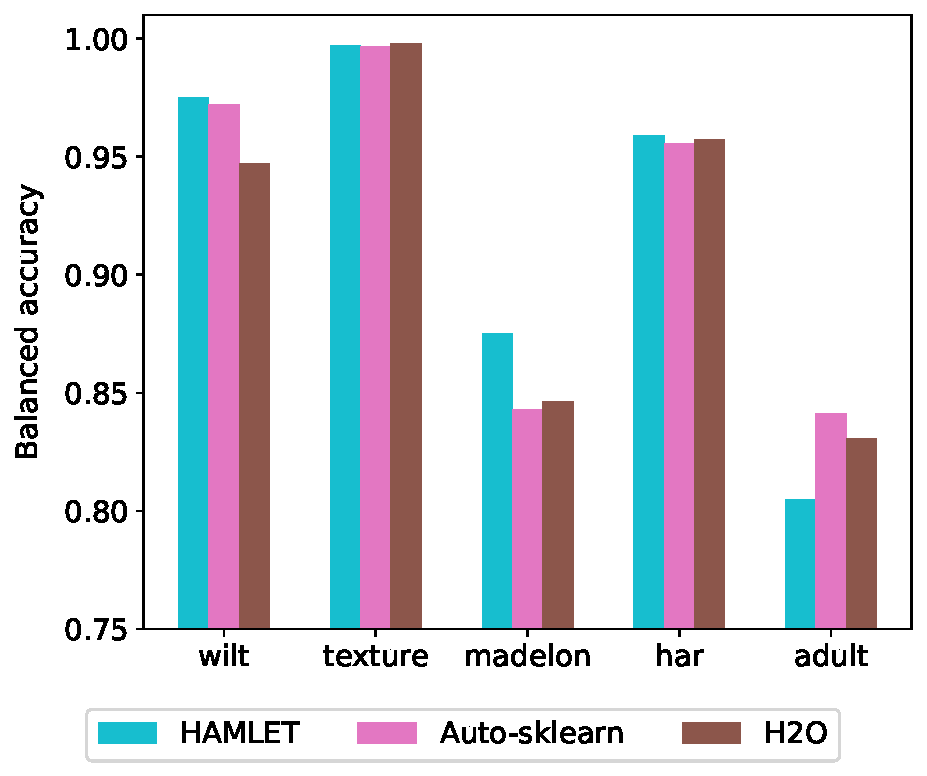
\includegraphics[scale=.45]{part-automl/chapter-supervised/img-hamlet/comparison.pdf}
%     \caption{Results assessing the performance of HAMLET w.r.t. Auto-sklearn \cite{feurer2019auto} and H2O \cite{ledell2020h2o}.}
%     \label{fig:comparison}
% \end{figure}


% \Cref{fig:comparison} compares HAMLET against two well-known AutoML frameworks: Auto-sklearn \cite{feurer2019auto} and H2O \cite{ledell2020h2o}.
% In four datasets out of five, HAMLET outperforms or is comparable to the two frameworks.
% Additionally, the added value of HAMLET is \textit{explainability}.
% Hamlet is a human-in-the-loop AutoML framework tailored to the needs of DS that (i) enables the injection of their experience into the exploration process as well as (ii) the spreading and sharing of knowledge bases that encode what DSs have understood by the optimization of their pipelines.


% \subsection{Conclusions and Future Work}\label{ssec:conclusion}

% Data platforms support Data Scientists in performing end-to-end data analysis; to this end, Machine Learning plays a primary role.
% However, the complexity and heterogeneity of (Automated) Machine Learning processes are leading Data Scientists to lose control over such processes.
% Human awareness about the constraints and solutions of Machine Learning tasks is a fundamental aspect to consider, and consequently, the Data Scientist should play a central role in the design of next-generation data platforms.

% According to this vision, we present HAMLET, a framework for Human-centered AutoML based on Logic and Structured Argumentation.
% Logic is exploited to structure the knowledge that the Data Scientist gathers while designing, modeling, and deploying a solution.
% The logical encoding of the knowledge provides a medium that is both human- and machine-readable and it allows an easy exploration and verification of all the constraints that may apply to the case at hand---it is overwhelming for the Data Scientist to correctly handle the vast amount of them.
% The preliminary evaluation of HAMLET shows promising results against state-of-the-art AutoML algorithms both in terms of effectiveness and efficiency, with argumentation introducing a small overhead with respect to the duration of the exploration process.

% The directions for future work are plentiful, among them:
% \begin{itemize}
%     \item[(i)] the recommendation of more constraints out of the explored search space (e.g., rare or negative patterns);
%     \item[(ii)] the support to heterogeneous constraints on hyperparameter domains;
%     \item[(iii)] the injection of meta-learning into our Logical Knowledge Base to better identify when and how the constraints should be applied (e.g., this can be done after testing HAMLET on a multitude of datasets);
%     \item[(iv)] the introduction of a visual metaphor (e.g., based on the Problem Graph) to help Data Scientists' understanding;
%     \item[(v)] the study of automatic resolution/recommendation of conflicting constraints, also depending on the rules already embedded in the Logical Knowledge Base.
% \end{itemize}

% 
\chapter{Effective Data-preprocessing Pipelines in Supervised Learning}
\label{data-centric-chap:supervised}

\begin{figure*}[t]
    \centering
    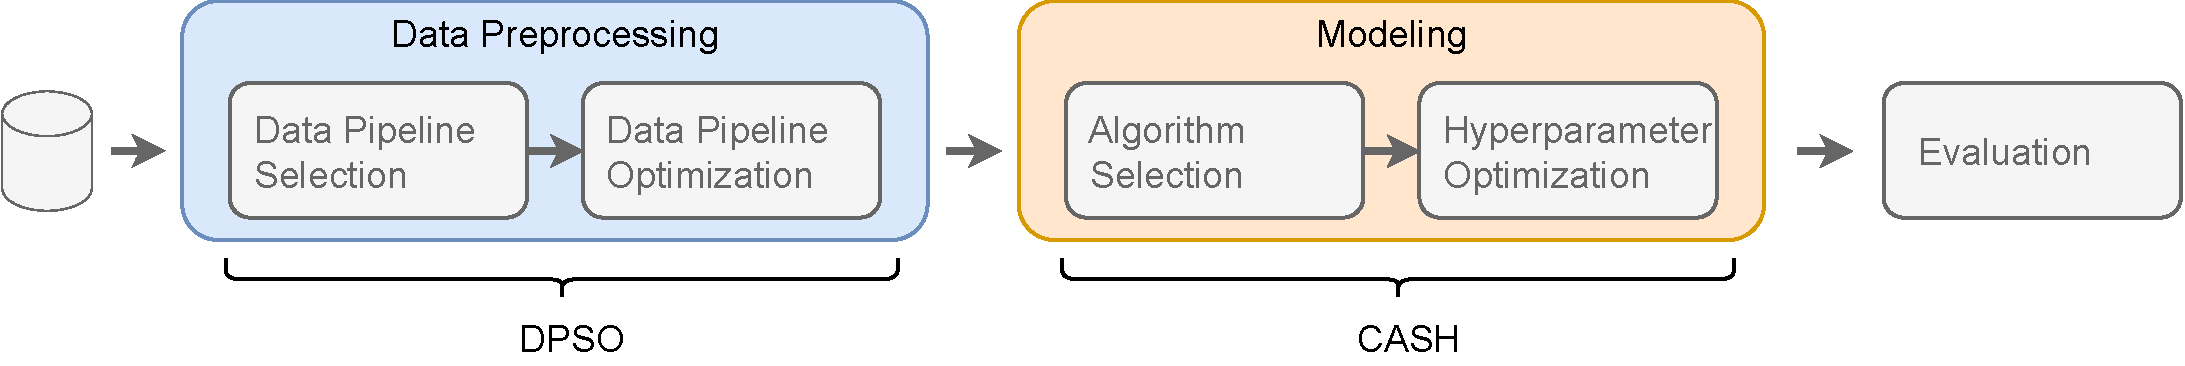
\includegraphics[width=1.0\textwidth]{chapters/data-centric/supervised/img/data-analytics-pipeline.pdf}
    \caption{Data analytics pipeline generation in a knowledge discovery process.}
    \label{effective-fig:data-analytics-pipeline}
\end{figure*}

To unleash the full potential of ML, data-centric AI focuses on shaping data according to the task and algorithm at hand.
With reference to the CRISP-DM process model,  \Cref{effective-fig:data-analytics-pipeline} summarizes the stages involved and the corresponding problems in the literature.
Firstly, data are extracted in a raw format from different sources and sifted out so that only a relevant subset is selected.
Next, during the pre-processing stage, the data pipeline selection and optimization (DPSO) \cite{Quemy19DOLAP} problem is tackled.
Once the data is transformed into the proper form, the modelling stage focuses on the combined algorithm selection and hyperparameter (CASH) optimization problem.
Finally, pipelines and algorithms
are evaluated over the dataset until an acceptable result is obtained.

It is well-known that the whole process requires expertise and is particularly challenging.
Particularly, data scientists spend most of their time on the heavily laborious work of pre-processing (i.e., around 50-80\% of the total \cite{Munson09Pre}).
Some AutoML frameworks \cite{auto_sklearn, mohr2018ml}, mix-in pre-processing during modelling optimization, but typically include very few transformations or do not consider all the necessary steps (e.g., imputation, rebalancing), thus in a way overlooking it.
Inspired from \cite{Munoz09DOLAP}, we contend that there is need for more data-centric techniques, encompassing all the steps of data pre-processing \cite{Vaisman14Book}.
Assistance is required in every phase \cite{Bilalli16IOTBD}.
By considering pre-processing as an integral component of the learning process, and carefully selecting and optimizing data pipelines, it is easy to obtain results that go beyond the ones obtained by only optimizing ML algorithms.

To briefly illustrate this, we perform an experiment on the well known \texttt{bank-marketing}\footnote{\url{https://archive.ics.uci.edu/ml/datasets/Bank+Marketing}} dataset, using HyperOpt \cite{HyperOptICML13} as an AutoML approach to optimize the parameters of three different ML algorithms, namely Naive Bayes (NB), K-Nearest Neighbor (KNN), and Random Forest (RF).
We provide an initial budget of 50 iterations for optimizing the hyperparameters of the algorithms, and after the 50th iteration, we fix the algorithm configuration to the best one achieved so far and start optimizing the pre-processing pipeline\footnote{This order is used only for the sake of illustration.}.
In \Cref{effective-fig:pre-processing-impact}, the ratio of the change in terms of accuracy (i.e., obtained after the i-th iteration to the baseline/default accuracy) is plotted against the number of different configurations visited by HyperOpt (i.e., iterations).
Observe that after the 11th iteration for NB and KNN, and after the 26th iteration for RF, the lines remain flat.
That is, from there on, no improvement is achieved by optimizing the hyperparameters of the algorithms until the 50th iteration is reached. At this point, a sudden jump is observed and the results start to improve again, going clearly beyond the ones obtained before, thanks to the optimizations performed now over the pre-processing pipeline.

\begin{figure}[t]
    \centering
    \includegraphics[width=0.7\textwidth]{chapters/data-centric/supervised/img/pre-processing-impact.pdf}
    \caption{Evolution of accuracy during the optimization process. The first 50 configurations optimize only the hyperparameters and after the 50th configuration, the pre-processing pipeline is optimized instead.}
    \label{effective-fig:pre-processing-impact}
\end{figure}

\paragraph{Challenges} Including pre-processing in the learning process heavily increases the search space, making the problem much harder.
DPSO entails two challenges that the data scientists have to undergo to find the most appropriate pipeline: (i) choose how to order the different pre-processing steps  (i.e., pipeline selection), and (ii) choose which transformations, with corresponding hyperparameters, should be adopted in the final implementation  (i.e., pipeline optimization).
To better distinguish between pipeline selection and its optimization, we follow the notation from \cite{Quemy20InfSystems}: a \textit{prototype} is the fixed and ordered sequence of pre-processing steps, its optimized instantiation of each transformation (with their hyperparameters) is known as \textit{executable pipeline}.

\paragraph{Contributions} The aim of this chapter is to study the two questions raised and propose a method for selecting effective pre-processing prototypes that, once optimized through some optimization technique (e.g., Bayesian optimization), improve the final result of the analysis.
To keep discussions and experiments simpler, we stick to supervised learning tasks.
The main contributions can be summarized as follows.
\begin{itemize}
    \item We empirically evaluate the impact of optimizing the exhaustive set of potential prototypes and find out that	there is no universal solution---i.e., prototype that works best for each dataset and algorithm considered.
    \item We define a method that given an ML algorithm and a set of pre-processing steps, is capable of generating the right order, obtaining effective pre-processing prototypes that are then instantiated via bayesian optimization.
    \item We suggest a meta-learning step (i.e., learning on top of learning) where the relationships between pre-processing transformations and dataset characteristics are learned in order to create rules that help with the initial instantiation of the prototypes.

	We exemplify our meta-learning study generating simple but not obvious and effective rules for two kinds of pre-processing steps, namely, Feature Engineering and Rebalancing.
    \item We perform a comprehensive evaluation by comparing the performance of optimizing prototypes generated following our method, and find out that:
    \begin{enumerate}
        \item with 24 times less time budget, our proposed pipelines obtain results whose median is above 90\% of the ones generated via exhaustive search.
        \item on average, in 73\% of the cases, splitting evenly the time budget between pre-processing and modelling outperforms the results of solely optimizing the latter.
    \end{enumerate}
	\item We deploy \textbf{AutoPrep}, a reproducibility framework for the automatic generation of effective pre-processing pipeline prototypes. Specifically, in \cite{giovanelli2023reproducible}, we introduce: (i) a detailed reproducibility protocol, (ii) software, and (iii) datasets in a self-contained environment.
	The experiments were run on several machines and confirmed all the inishts in this chapter.
\end{itemize}

The remaining of this chapter is organized as follows:
\Cref{effective-sec:related-work} discusses the related work,
\Cref{effective-sec:methodology} presents our method of generating effective pipelines,
\Cref{effective-sec:evaluation} provides an extensive evaluation of the pipelines created using our proposed method and, finally, \Cref{effective-sec:conclusions} provides the conclusions and future work.


\section{Related Works}
\label{effective-sec:related-work}
At the beginning, the AutoML community followed the AI trend of contributing under a more algorithmic perspective, focusing on modelling---i.e., the resolution of the CASH problem.
Recently however, the direction has shifted towards designing systems that additionally or specifically provide user assistance in the data pre-processing step---i.e., solving the DPSO problem.
We can categorize works according to the optimization policy \cite{quemy2019data} they adopt.
On the one hand, some automate data pre-processing via split-like policies---i.e., addressing DPSO in isolation from CASH (\Cref{effective-ssec:dpso}).
On the other hand, some consider optimizing DPSO along with CASH, adopting a joint policy---data pre-processing in synergy with modelling (\Cref{effective-ssec:dpso-cash}).

\subsection{Optimization with Split-like Policies}
\label{effective-ssec:dpso}

In \cite{Quemy20InfSystems}, authors demonstrate the impact of optimizing the pre-processing pipelines, but considering only a single fixed prototype and only a few datasets.
However, as we have already seen (\Cref{effective-sec:eval-universal-pipeline}), a single fixed prototype cannot perform best for every dataset.

In PRESISTANT \cite{presistant18CSI,presistant18CAISE,presistant19DKE}, authors tackled the problem of recommending pre-processing transformations to non-expert users.
They identify the pre-processing transformations and rank them in advance, based on their potential impact to the final analysis.
However, they do not consider pre-processing pipelines, but only single transformations, expecting that the analyst applies the process iteratively.

In ActiveClean \cite{ActiveClean16PVLDB}, authors define a method that aims at prioritizing the cleaning of records that are more likely to affect the results of the analysis, assuming that the latter belongs to the class of convex loss models (i.e., linear regression and SVMs).
Hence, instead of recommending the transformations to be applied, the system recommends the subset of data that needs to be cleaned at a given point.
The type of pre-processing to be applied is left to the user, assuming that the user is an expert.

In Learn2Clean \cite{Berti19WWW}, based on a reinforcement learning technique, for a given dataset and an ML model, an optimal sequence of pre-processing transformations is generated so that the quality of the ML model is maximized.
Yet, similarly to \cite{Quemy20InfSystems}, the pipeline prototype is fixed in advance.

In Alpine Meadow \cite{Shang19SIGMOD}, authors follow a similar approach to ours in that they define two steps for the pre-processing phase. One, the so-called \textit{logical pipeline plan}, which is roughly equivalent to the \textit{prototype} defined in this work, and the second the \textit{physical pipeline plan} which translates to \textit{executable pipelines} used in this work.
The physical plan is generated through a combination of Bayesian optimization, meta-learning, and multi-armed bandits.
For the logical plans, they rely on rules but without clear evidence on how they are generated.
Moreover, it is not clear whether the logical plan is fixed as in \cite{Quemy20InfSystems} and if some further adjustment from the user is required.

\subsection{Optimization with a Joint Policy}
\label{effective-ssec:dpso-cash}
Auto-sklearn \cite{Feurer15AutoSklearn} is based on the popular Python library scikit-learn.
The authors, inspired by Auto-Weka, address the problem with the Sequential Model-based Algorithm Configuration (SMAC).
Furthermore, they improve the approach by adding a meta-learning phase (i.e., learning on top of learning) at the beginning and an ensemble technique at the end.
Meta-learning leverages previous ML experiments and learns promising configurations to warm-start (i.e., boost the convergence) the Bayesian Optimization.
Ensemble techniques merge predictions from multiple ML models to statistically outperform the base models.
Yet, they consider a small set of transformations and also consider a single fixed prototype.

TPOT \cite{Olson16Tpot} is a tree-based pipeline optimization tool using genetic programming while requiring little to no expertise from the user.
In TPOT however, they only consider one transformation inside the optimization process (i.e., Feature Engineering).

ML-Plan \cite{mohr2018ml} uses hierarchical planning, a particular form of AI planning, to propose a solution to both the pre-processing and the modeling phases.
As in context-free grammars, there are complex tasks (non-terminal symbols) that are derived as long as primitive tasks (terminal symbols) are not obtained.
Typically, standard graph search algorithms (e.g., depth-first search, best-first search, etc.) are employed to solve such problems.
ML-Plan successively creates solutions in a global search instead of changing given solutions in a local search. However, due to the problem constraints, they adopt a randomized best-first search, randomly choosing the solution path.

AutoBazaar \cite{AutoBazaar} is a Python open-source tool.
Like in ML-Plan \cite{mohr2018ml}, both pre-processing and modeling phases are covered.
Here the last step of a prototype is the machine learning algorithm.
The approach involves two different steps.
Firstly, a \textit{catalog} proposes a collection of prototypes (with an ML algorithm as last step) based on the task and the dataset itself.
Secondly, the optimization process starts tuning the prototypes until either the time budget is expired or the prototypes are all optimized.
In particular, a \textit{selector} and a \textit{tuner} work in synergy.
The former decides which prototype should be optimized next.
Such a task is treated as a multi-armed bandit problem.
As to the tuner, bayesian optimization is chosen.
At the end, the prototype that achieved the higher accuracy is elected.
However, AutoBazaar strictly depends on the catalog.
Such a component memorizes all the possible primitives and supported tasks.
The prototypes are hard-coded for each task.
Thus, it is neither flexible nor maintainable.
If a task is not implemented, the approach cannot suggest a solution.

To summarize, full automation of data analytics has been the ultimate goal of many research works.
Yet, such automation has shown to be computationally expensive, mainly due to the search space involved (i.e., pre-processing and mining operators).
Therefore, the usability of these approaches in realistic scenarios is sometimes limited.
Our approach of finding a set of effective prototypes can be seen as complementary to these solutions, since it helps in pruning the large space and guiding the search, hence reducing their cost.

\section{Effective Data Pre-processing Pipeline Generation}
\label{effective-sec:methodology}

We aim to find the best data pipeline (i.e., with higher performance) for the dataset $\altmathcal{D}$ and the ML algorithm $A$ considered, hence solving DPSO.
Let us refresh the formalization of interest.

Each transformation $T$ exposes a set of $K$ hyperparameters, producing the Cartesian product $\Lambda_T = \Lambda_1 \times \dots \times \Lambda_K$.
A pre-processing \textit{step} $S$ can be instantiated from several alternative transformations, hence $\Lambda_S = \Lambda_{T_1} \cup \ldots \cup \Lambda_{T_{|S|}} \cup \lambda_s$, with $\lambda_s$ a new root-hyperparameter that selects the transformation.
The problem exacerbates when steps are combined together into data pipelines.
Indeed, the complete search space for our optimization problem is defined as $\Lambda_P = \Lambda_{S_1} \times \ldots \times \Lambda_{S_{|P|}} \times \lambda_p$, with $\lambda_p$ as yet another root-hyperparameter to select -- this time -- the order between the transformations (translating into the disjoint union of all partial permutations).

To mitigate the problem's complexity, we distinguish between pipeline selection and its optimization.
Specifically, following the notation from \cite{quemy2019data}:
pipeline selection aims at finding promising \textit{prototypes}, i.e. fixed and ordered sequence of pre-processing steps, pipeline optimization instantiates the best \textit{executable pipeline}, i.e. assigning a transformation (along with the hyperparameters) to each pre-processing step.

\begin{figure*}[t]
    \centering
    \includegraphics[width=1.0\textwidth]{chapters/data-centric/supervised/img/bpmn.pdf}
    \caption{A method for generating effective pre-processing pipelines}
    \label{effective-fig:methodology}
\end{figure*}

\Cref{effective-fig:methodology} sketches the proposed methodology, some of the phases are generic and thus can be applied regardless of the context, and yet others are specific (i.e., ML framework or dataset characteristics).
According to \cite{Quemy20InfSystems}, we break the combinatorial problem into two workflows: (i) studying pre-processing steps in pairs for generating effective prototypes and then (ii) feeding them to an optimizer (e.g., we use the SMBO \cite{HyperOptICML13} variant) for their actual instantiation.

\paragraph{Effective Prototypes Generation} The proposed method starts with the selection of the ML library (\Cref{effective-ssec:select-framework}).
This allows to consider solely the steps for which their implementation is available.
Besides, with such a choice, we are also provided with a set of \textit{framework-related rules} (\Cref{effective-ssec:rules-framework}), constraining the possible orderings of the steps (e.g., in scikit-learn, Imputation has to be the first step in the prototype).
These rules are in the form of precedences of pre-processing steps (i.e. orderings that involve two steps at a time;  e.g., Imputation before Normalization).
Next, the flow on top continues with a study
aiming to find the correct/meaningful orderings according to
the behavior of the transformations in each step.
As a result, this generates a set of \textit{heuristic rules} (\Cref{effective-ssec:rules-heuristics}) that restrict the space of possible precedences.
Afterward, for the pairs for which an order cannot be clearly devised, an additional empirical study is proposed.
This study relies on a test bed of representative datasets.
The output is a set of \textit{empirically-learned rules} (\Cref{effective-ssec:rules-learned}) that determines yet other precedences, namely promising orderings that would potentially positively impact the final result of the analysis.
However, even after this phase, for some pairs of pre-processing steps, a precedence order may not be found.
These are pairs for whom the order is relevant but cannot be decided in advance, thus all their permutations need to be present.
Finally, a step of composition follows  (\Cref{effective-ssec:composition}), where given the overall set of devised rules (i.e., \textit{framework-related}, \textit{heuristic} and \textit{empirically-learned}), the pre-processing steps are composed into a set of valid and potentially effective prototypes.

More formally, when combining two different pre-processing steps, it is important to check if, (i) the input and output types of the steps are compatible, (ii) the combination makes sense, and (iii) the combination provides good results for the analysis.
As a result, when chaining a pair of steps, the following precedence relationships arise:
\begin{enumerate}
    \item Compatible/Incompatible. Depending on whether the representation output of the first step is accepted as the representation input of the second one (compatible), or not (incompatible).
    \item Meaningful/Meaningless. Depending on whether the precedence between them makes sense based on generic knowledge (i.e., based on the literature) over the behaviour of transformations (meaningful), or not (meaningless).
    \item Promising/Unpromising. Depending on whether the precedence between them is expected to provide a positive impact on the final result of the analysis (promising), or not (unpromising).
\end{enumerate}

Attending to the relationships between its steps, a prototype can be described as either \textit{compatible}, \textit{well-formed}, or \textit{effective}.
A prototype is defined to be \textit{compatible} if all its precedence relationships are available in the ML framework at hand.
It is defined as \textit{well-formed} if all its precedence relationships are both compatible and meaningful.
Finally, it is defined as \textit{effective} if all its precedence relationships are compatible, meaningful, and promising at the same time.
In fact, the goal of this flow is to find \textit{effective prototypes}.

\paragraph{Warm-starting via Meta-learning} Once the prototype is constructed, the flow running in parallel is proposed to help with its instantiation.
It consists of a meta-learning step  (\Cref{effective-ssec:meta-learning}), where a set of ML experiments (e.g., pre-processing and classification algorithm runs) are used as training data to predict promising transformations for a pre-processing step.
These rules extract knowledge from past experiments and are complementary to the rules obtained in the first flow.
This practice is called warm-starting,
They would be used, for example, to ease the cold start problem in the prototype instantiation phase  (\Cref{effective-ssec:prototype-insta}).

We propose a generic methodology.
However, to keep the reader from losing, we will illustrate our use case and corresponding findings along with the explanation of the methodology.

\subsection{Selection of Data Pre-Processing Steps and Transformations}
\label{effective-ssec:select-framework}

The first task in the process consists of selecting the data pre-processing steps and their available transformations according to the selected ML library.

\paragraph{Use case}
For our experiments, we selected the pre-processing steps, transformations and hyperparameters from those available in the scikit-learn library\footnote{\url{https://scikit-learn.org}} (\Cref{effective-tbl:transformations}).
\textit{Input} denotes the compatible feature type for a given pre-processing step and can be continuous (CO) -- when it represents measurements on some continuous scale -- or categorical (CA)---when it represents information about some categorical or discrete characteristics.
Similarly, \textit{Output} denotes the type of the features after a pre-processing step is applied.

\begin{itemize}[noitemsep,topsep=0pt]
\item{Encoding ($E$).} The process of transforming categorical features into continuous ones (here, we refer solely to the encoded representation, not the semantic).
\item{Normalization ($N$).} The process of normalizing continuous features such that their values fall in the same range.
\item{Discretization ($D$).} The process of transforming continuous features into categorical ones.
\item{Imputation ($I$).} The process of imputing missing values.
\item{Rebalancing ($R$).} The process of adjusting the class distribution of a dataset (i.e. the ratio between the different classes/categories represented).
\item{Feature Engineering ($F$).} The process of defining the set of relevant features to be used in model training.
\end{itemize}

Finally, \textit{transformations} denotes the actual instantiation for the step, and it can be tuned using its \textit{hyperparameters}.


\begin{table}[!t]
\renewcommand{\arraystretch}{0.3}
\footnotesize
\caption{List of transformations applicable to categorical or continuous data types.}
\centering
\begin{threeparttable}

\begin{tabular}{@{}p{30mm}lll>{\ttfamily}l@{}}
\toprule
Pre-processing Step& Input & Output & Transformation & \textnormal{Hyperparameters}
\\	\cmidrule[.1em]{1-5}

Encoding ($E$)  & CA & CO & Ordinal & -  \\ \cmidrule[.05em]{4-5} & & & One Hot & - \\
\cmidrule[.1em]{1-5}

Normalization ($N$) & CO & CO & Standard Scaler & with\_mean:[True,False]\\ \cmidrule[.05em]{4-5} & & & & with\_std:[True,False] \\ \cmidrule[.05em]{4-5}
&  &  & Power Transform & -\\ \cmidrule[.05em]{4-5}
&  &  & MinMax Scaler & -\\ \cmidrule[.05em]{4-5}
&  &  & Robust Scaler & quantile\_range:[(25,75),(10,90),(5,95)]\\ \cmidrule[.05em]{4-5} & & & & with\_centering:[True,False]\\ \cmidrule[.05em]{4-5} & & & & with\_scaling:[True,False] \\
\cmidrule[.1em]{1-5}

Discretization ($D$) & CO & CA & KBins & n\_bins:[3,5,7]\\ \cmidrule[.05em]{4-5} & & & & encode:[`onehot',`onehot-dense',`ord.']\\ \cmidrule[.05em]{4-5} & & & & strategy:[`uniform',`quant.',`kmeans']\\	\cmidrule[.05em]{4-5}
&  &  & Binarization  & threshold: [0, 0.5, 2, 5]\\	\cmidrule[.1em]{1-5}

Imputation ($I$) & CA/CO & CA/CO  & Univariate & strategy:[`most\_freq.','constant'] \\	\cmidrule[.05em]{4-5}
 & &  & Multivariate & initial\_strategy:[`most\_freq',`const.']\\ \cmidrule[.05em]{4-5} & & & & order:[`asc',`dsc',`rom',`arab',`rand'] \\	\cmidrule[.1em]{1-5}

Rebalancing ($R$)* &CA/CO  & CA/CO & Near Miss & n\_neighbors:[1,2,3]\\ \cmidrule[.05em]{4-5}
%&  &  & \textcolor{red}{Condensed KNN} & \textcolor{red}{n\_neighbors:[1,2,3]} \\ \cmidrule[.05em]{4-5}
&  &  & SMOTE & k\_neighbors:[5,6,7]\\	\cmidrule[.1em]{1-5}

Feat. Eng. ($F$) & CA/CO & CA/CO & PCA & n\_components:[1,2,3,4]\\ \cmidrule[.05em]{4-5}
&  &  & Select K Best & k:[1,2,3,4]\\ \cmidrule[.05em]{4-5}
&  &  & PCA + Select K Best  & n\_components:[1,2,3,4]
\\ \cmidrule[.05em]{4-5} & & & & k:[1,2,3,4]\\	\bottomrule%\cmidrule[.1em]{1-5}
\end{tabular}
\begin{tablenotes}
\footnotesize
\item CA - categorical, CO - continuous.
\item *All transformations except Rebalancing are taken from scikit-learn.
\end{tablenotes}
\end{threeparttable}
\label{effective-tbl:transformations}
\end{table}

\begin{table*}[!t]
    \caption{
        Precedence order between pairs of pre-processing steps, represented independently for each phase.
        }
    \renewcommand{\arraystretch}{0.3}
    \footnotesize
    \begin{center}
    \subfloat[Compatible precedence.]{
    \begin{tabular}{@{}lcccccc}
    \toprule
     & $\boldsymbol{E}$ & $\boldsymbol{N}$ & $\boldsymbol{D}$ & $\boldsymbol{I}$ & $\boldsymbol{R}$ & $\boldsymbol{F}$
    \\	\cmidrule[.1em]{1-7}
    $\boldsymbol{E}$ & \cellcolor{gray!25} & \texttt{1} & \texttt{1} & \texttt{\texttt{0}} & \texttt{1} & \texttt{1} \\	\cmidrule[.1em]{1-7}
    $\boldsymbol{N}$ & \texttt{0} & \cellcolor{gray!25}  & \texttt{0} & \texttt{0} & \texttt{0} & \texttt{0} \\	\cmidrule[.1em]{1-7}
    $\boldsymbol{D}$ & \texttt{0} & \texttt{0} & \cellcolor{gray!25}  & \texttt{0} & \texttt{0} & \texttt{0} \\	\cmidrule[.1em]{1-7}
    $\boldsymbol{I}$ & \texttt{1} & \texttt{0} & \texttt{1} & \cellcolor{gray!25}  & \texttt{1} & \texttt{1} \\	\cmidrule[.1em]{1-7}
    $\boldsymbol{R}$ & \texttt{0} & \texttt{0} & \texttt{0} & \texttt{0} & \cellcolor{gray!25}  & \texttt{0} \\	\cmidrule[.1em]{1-7}
    $\boldsymbol{F}$ & \texttt{0} & \texttt{0} & \texttt{0} & \texttt{0} & \texttt{0} & \cellcolor{gray!25}
    \\	\bottomrule
    \end{tabular}}
    \qquad% --- set horizontal distance between tables here
    \subfloat[Meaningful precedence.]{%
    \begin{tabular}{@{}lcccccc}
    \toprule
    & $\boldsymbol{E}$ & $\boldsymbol{N}$ & $\boldsymbol{D}$ & $\boldsymbol{I}$ & $\boldsymbol{R}$ & $\boldsymbol{F}$
    \\	\cmidrule[.1em]{1-7}
    $\boldsymbol{E}$ & \cellcolor{gray!25} & \texttt{0} & \texttt{0} & \texttt{0} & \texttt{0} & \texttt{0} \\	\cmidrule[.1em]{1-7}
    $\boldsymbol{N}$ & \texttt{0} & \cellcolor{gray!25}  & \texttt{X} & \texttt{0} & \texttt{1} & \texttt{0} \\	\cmidrule[.1em]{1-7}
    $\boldsymbol{D}$ & \texttt{0} & \texttt{X} & \cellcolor{gray!25}  & \texttt{0} & \texttt{0} & \texttt{0} \\	\cmidrule[.1em]{1-7}
    $\boldsymbol{I}$ & \texttt{1} & \texttt{1} & \texttt{1} & \cellcolor{gray!25}  & \texttt{1} & \texttt{1} \\	\cmidrule[.1em]{1-7}
    $\boldsymbol{R}$ & \texttt{0} & \texttt{0} & \texttt{0} & \texttt{0} & \cellcolor{gray!25}  & \texttt{0} \\	\cmidrule[.1em]{1-7}
    $\boldsymbol{F}$ & \texttt{0} & \texttt{0} & \texttt{0} & \texttt{0} & \texttt{0} & \cellcolor{gray!25}
    \\	\bottomrule
    \end{tabular}}
    \qquad% --- set horizontal distance between tables here
    \subfloat[Promising precedence.]{%
    \begin{tabular}{@{}lcccccc}
    \toprule
    & $\boldsymbol{E}$ & $\boldsymbol{N}$ & $\boldsymbol{D}$ & $\boldsymbol{I}$ & $\boldsymbol{R}$ & $\boldsymbol{F}$
    \\	\cmidrule[.1em]{1-7}
    $\boldsymbol{E}$ & \cellcolor{gray!25} & \texttt{0} & \texttt{0} & \texttt{0} & \texttt{0} & \texttt{0} \\	\cmidrule[.1em]{1-7}
    $\boldsymbol{N}$ & \texttt{0} & \cellcolor{gray!25} & \texttt{0} & \texttt{0} & \texttt{0} & \texttt{1} \\	\cmidrule[.1em]{1-7}
    $\boldsymbol{D}$ & \texttt{0} & \texttt{0} & \cellcolor{gray!25} & \texttt{0} & \texttt{0} & \texttt{1} \\	\cmidrule[.1em]{1-7}
    $\boldsymbol{I}$ & \texttt{0} & \texttt{0} & \texttt{0} & \cellcolor{gray!25} & \texttt{0} & \texttt{0} \\	\cmidrule[.1em]{1-7}
    $\boldsymbol{R}$ & \texttt{0} & \texttt{0} & \texttt{0} & \texttt{0} & \cellcolor{gray!25} & \texttt{0} \\	\cmidrule[.1em]{1-7}
    $\boldsymbol{F}$ & \texttt{0} & \texttt{0} & \texttt{0} & \texttt{0} & \texttt{0} & \cellcolor{gray!25}
    \\	\bottomrule
    \end{tabular}}
    \end{center}
    \begin{tablenotes}
    \centering
    \scriptsize
    \item$\boldsymbol{E}$ - Encoding; $\boldsymbol{N}$ - Normalization; $\boldsymbol{D}$ - Discretization; $\boldsymbol{I}$ - Imputation; $\boldsymbol{R}$ - Rebalancing; $\boldsymbol{F}$ - Feature Engineering. \item \texttt{1} - a precedence edge exists between the row and the column, \texttt{0} - a precedence edge does not exist between the row
    \item and the column, \texttt{X} - the combination is meaningless.
    \end{tablenotes}
    \label{effective-tbl:rules}
    \end{table*}

\subsection{Extraction of Compatible Precedences}
\label{effective-ssec:rules-framework}

Once the implementation framework is selected, one needs to study it and see if there exist constraints that limit the interaction between the pre-processing steps.
For instance, applying a step may actually invalidate the application of another one, because the compatibility of them is dependent on the selected ML framework.
We aim at detecting a set of implicit rules that are shown through an adjacency matrix, corresponding to a precedence graph as those in \Cref{effective-tbl:rules}.
Each cell $a_{ij}$ denotes a precedence relationship between the row $i$ and column $j$.
Hence, \texttt{1} means that an edge exists between the transformation in the row and the transformation in the column, whereas \texttt{0} means that such an edge does not exist, hence a precedence order is not established for that pair.

\paragraph{Use case}
We studied the pre-processing steps implemented in Scikit-learn, the discovered rules are shown through the adjacency matrix in \Cref{effective-tbl:rules}a.
For example, most Scikit-learn steps cannot be applied in the presence of missing values.
This is why in every pair of them where Imputation is involved, except the one with Normalization\footnote{Normalization transformations are the only ones that Scikit-learn can apply on datasets with missing values.}, Imputation goes first.
Furthermore, Scikit-learn steos are applied only to all compatible features of a given dataset.
Generally, categorical features are physically represented as strings and continuous features as numbers.
However, a transformation that is meant to be applied, say to continuous features, cannot be applied over a dataset that contains both continuous and categorical features (i.e., a dataset containing both numbers and strings); Scikit-learn cannot deal with arrays of mixed types.
In that case, all the categorical features need to be encoded into numeric representations, even if they represent a categorical value.
That is, a value can be a number but represent a category.
This is what happens when Normalization and Discretization are meant to be applied to a dataset containing mixed types of features.
In order for them to be applied to datasets of mixed types, an Encoding transformation needs to be applied first.
A similar constraint is imposed when considering Rebalancing and Feature Engineering, since these steps do not accept inputs containing strings (i.e., representing a categorical type).
For the rest of the pairs, there are no constraints imposed by the framework, thus any ordering is permitted, reflected by a \texttt{0} in \Cref{effective-tbl:rules}a.
The graph obtained in this case exclusively corresponds to the limitations of Scikit-learn (as a matter of fact, if another framework were to be chosen, it may have looked differently).

\subsection{Discovery of Well-formed Precedences}
\label{effective-ssec:rules-heuristics}
Once we have derived precedences based on the constraints of the framework, we can study the precedence independently and find \textit{meaningful pairs}.
That is, for every given pair, we want to find the relative order based on generic domain-independent knowledge (i.e., literature) about pre-processing steps and their applicability.
To this end, some of the constraints imposed by the framework may be contradicted here, but this is resolved in the last step of the proposed method (\Cref{effective-ssec:composition}).
Briefly, in a combination where Imputation is involved, it is advised to apply Imputation first.
Next, Encoding makes sense to be combined in any order with the rest of the transformations, except Imputation.
Combining Discretization with Normalization does not make sense, due to the fact that after the Discretization step, continuous features are transformed into categorical ones, and hence Normalization cannot be applied.
Similarly, applying Normalization first, changes the scale of the values and hence impacts the Discretization step.
Finally, a meaningful precedence can be derived when combining Normalization with Rebalancing.
In this case, Normalization should be applied first, since otherwise Rebalancing would impact the scale of the values to be normalized.

\paragraph{Use case}
\Cref{effective-tbl:rules}b shows the heuristic rules obtained considering domain-independent knowledge about the steps \cite{BookExploratoryDM03Dasu}.
In comparison with the results from \Cref{effective-tbl:rules}a, observe that the constraints on the Imputation still hold: when combining it ith another step, Imputation should go first.
This time even when combining it with Normalization---note the difference with \Cref{effective-tbl:rules}a.
The constraints of Encoding are however not present in \Cref{effective-tbl:rules}a, hence not considering the framework, Discretization combined with Encoding is a meaningful combination---when a mixed type dataset is considered, but incompatible from the point of view of Scikit-learn.

\subsection{Empirical-learning of Promising Precedences}
\label{effective-ssec:rules-learned}

The two previously proposed phases (i.e., \textit{framework-related} and \textit{heuristic rules}), do not guarantee that each pair of steps will obtain a precedence order.
Therefore, for those cases left out, a third viewpoint should be considered.
That of learning a promising order by empirically studying the impact of the combinations on the final result of the analysis, using different supervised problems in the training.
For every selected pair of pre-processing steps, for a given ML algorithm, we propose to check which order of the pair improves most the performance (e.g., accuracy) of the algorithm over a set of datasets (preferably from different domains).
Like this, for each dataset, we can get a precedence order that gives better results (i.e., promising precedence) in terms of the loss.


\begin{algorithm*}[!h]
	\caption{Find a promising prototype for steps $S_1$ and $S_2$}
	\label{effective-alg:learned-rules}
	\begin{algorithmic}[1]
		\Require $\altmathcal{D}_{train}$, $\altmathcal{D}_{valid}$, $A$, $\altmathcal{L}$ $S_1$, $S_2$ \Comment{dataset split for train and validation, classification algorithm, loss function, two different pre-processing steps}
		% \Require \indent$S_1\rightarrow S_2$, $S_2 \rightarrow S_1$ \Comment{precedence orders of a pair of transformations}
		\State $\altmathcal{L}_{\varnothing} = \altmathcal{L}(A(\altmathcal{D}_{train}), \altmathcal{D}_{valid})$ \Comment{get baseline performance of algorithm $A$ on $\altmathcal{D}$}
		\State $P_1 = \langle S_1, S_2 \rangle, P_2 = \langle S_2, S_1 \rangle$ \Comment{define two prototypes}
		\State $P_{1_{\lambda}} = SMBO(\langle P_1, A \rangle(\altmathcal{D}_{train}), \altmathcal{D}_{valid})$ \Comment{optimize the 1st prototype and get the best pipe}
		\State $\altmathcal{L}_{P_1} = \altmathcal{L}(\langle P_{1_{\lambda}}, A \rangle(\altmathcal{D}_{train}), \altmathcal{D}_{valid})$ \Comment{get the corresponding loss}
		\State $P_{2_{\lambda}} = SMBO(\langle P_2, A \rangle(\altmathcal{D}_{train}), \altmathcal{D}_{valid})$
		\Comment{optimize the 2nd prototype and get the best pipe}
		\State $\altmathcal{L}_{P_2} = \altmathcal{L}(\langle P_{2_{\lambda}}, A \rangle(\altmathcal{D}_{train}), \altmathcal{D}_{valid})$ \Comment{get the corresponding loss}
		% \State $[pipeline_{S_2\rightarrow S_1},acc_{S_2\rightarrow S_1}] = SMBO(S_2\rightarrow S_1,d, a)$
		% \Comment{get pipeline and accuracy for $S_2\rightarrow S_1$}
		% \If{\textit{IsValid}($acc_{S_1\rightarrow S_2},acc_{S_2\rightarrow S_1},acc_{baseline}$)}
		\If{$P_{1_{\lambda}}, P_{2_{\lambda}}$ are valid w.r.t. $\altmathcal{L}_{\varnothing}, \altmathcal{L}_{P_1}, \altmathcal{L}_{P_2}$}
        \Comment{see \Cref{effective-tbl:validation-rules} for the rules applied}
        \State \Return Best of $P_1$ and $P_2$
        \Comment{see column \textit{Winner prototype} in \Cref{effective-tbl:validation-rules}}
		\Else
		\State \Return $\varnothing$
		\EndIf
	\end{algorithmic}
\end{algorithm*}

\subsubsection{Experimental Learning Design}
To find a promising precedence order between a given pair of pre-processing steps $S_1$ and $S_2$, we propose \Cref{effective-alg:learned-rules}.
Let us consider a dataset split into $\altmathcal{D}_{train}$ and $\altmathcal{D}_{valid}$, a ML algorithm $A$, and a loss function $\altmathcal{L}$.
We first calculate $\altmathcal{L}_{\varnothing}$ as the loss of the ML algorithm $A$ over the original non-transformed dataset (line 1).
Afterward, to compute the impact of each possible prototype $P_1$ and $P_2$ (line 2), we leverage SMBO to find their optimized executable pipelines (line 3 and 5), and the losses of the ML algorithm (with default configuration) over the datasets transformed using the respective pipelines (line 4 and 6).
Based on the comparison between the respective optimized pipelines, we get the winner (line 7).
However, beforehand (line 6), we perform a validity check.
This is because when optimizing a pre-processing pipeline, SMBO may not instantiate a step with no transformation at all (i.e., represented with a $\varnothing$ symbol).
Hence, given a pair of pre-processing steps, where one or both of them may not be instantiated, SMBO may generate 16 possible scenarios.
They are listed in \Cref{effective-tbl:validation-rules}, and make up the validation rules for \Cref{effective-alg:learned-rules}.

\begin{table*}[t]
	\footnotesize
	\centering
	\begin{threeparttable}
	\caption{
		Validation rules.
		}
	\begin{tabular}{lp{2.3cm}p{2.3cm}p{2cm}p{2cm}p{2.5cm}}
	\toprule
	Nr. & Ex. Pipeline $P_{1_{\lambda}}$ & Ex. Pipeline $P_{2_{\lambda}}$ & Valid result & Valid score & Winner prototype\\\toprule
			1. &$\langle \varnothing, \varnothing \rangle$ & $\langle \varnothing, \varnothing \rangle$ & Draw          & $\altmathcal{L}_{\varnothing}$ &  Baseline \\ \hline
			2. &$\langle \varnothing, \varnothing \rangle$ & $\langle S_{2_{\lambda}}, \varnothing \rangle$ & Draw          & $\altmathcal{L}_{\varnothing}$ & Baseline \\ \hline
			3. &$\langle \varnothing, \varnothing \rangle$ & $\langle \varnothing, S_{1_{\lambda}} \rangle$ & Draw          & $\altmathcal{L}_{\varnothing}$ & Baseline \\ \hline
			\multirow{2}{*}{4.} &\multirow{2}{*}{$\langle \varnothing, \varnothing \rangle$} & \multirow{2}{*}{$\langle S_{2_{\lambda}}, S_{1_{\lambda}} \rangle$} & Draw & $\altmathcal{L}_{\varnothing}$ & Baseline \\
			& & & $P_{2_{\lambda}}$ & $\altmathcal{L}_{P_2}$ & $P_2$\\ \hline
			5. & $\langle \varnothing, S_{2_{\lambda}} \rangle$ & $\langle \varnothing, \varnothing \rangle$ & Draw          & $\altmathcal{L}_{\varnothing}$ & Baseline \\ \hline
			\multirow{3}{*}{6.} & \multirow{3}{*}{$\langle \varnothing, S_{2_{\lambda}} \rangle$} & \multirow{3}{*}{$\langle S_{2_{\lambda}}, \varnothing \rangle$} & Draw &  \multirow{3}{*}{$\altmathcal{L}_{S_2}$}  & $S_2$ \\
			& & & $P_{1_{\lambda}}$ & & $S_2$ \\
			& & & $P_{2_{\lambda}}$ & & $S_2$ \\ \hline
			7. &$\langle \varnothing, S_{2_{\lambda}} \rangle$ & $\langle \varnothing, S_{1_{\lambda}} \rangle$ & Draw & $\altmathcal{L}_{S_2}$ or $\altmathcal{L}_{S_1}$ & $S_{1}\,or\, S_2$ \\ \hline
			\multirow{2}{*}{8.} & \multirow{2}{*}{$\langle \varnothing, S_{2_{\lambda}} \rangle$} & \multirow{2}{*}{$\langle S_{2_{\lambda}}, S_{1_{\lambda}} \rangle$} & Draw & $\altmathcal{L}_{S_2}$ & $S_2$\\
			& & & $P_{2_{\lambda}}$ & $\altmathcal{L}_{P_2}$ & $P_2$ \\ \hline
			9. & $\langle S_{1_{\lambda}}, \varnothing \rangle$ & $\langle \varnothing, \varnothing \rangle$ & Draw & $\altmathcal{L}_{\varnothing}$ & Baseline \\ \hline
			10. & $\langle S_{1_{\lambda}}, \varnothing \rangle$ & $\langle S_{2_{\lambda}}, \varnothing \rangle$ & Draw & $\altmathcal{L}_{S_1}$ or $\altmathcal{L}_{S_2}$ & $S_{1}\,or\, S_2$ \\ \hline
			\multirow{3}{*}{11.} & \multirow{3}{*}{$\langle S_{1_{\lambda}}, \varnothing \rangle$} & \multirow{3}{*}{$\langle \varnothing, S_{2_{\lambda}} \rangle$} & Draw & \multirow{3}{*}{$\altmathcal{L}_{S_1}$} & $S_1$\\
			& & & $P_{1_{\lambda}}$ & & $S_1$\\
			& & & $P_{2_{\lambda}}$ & & $S_1$\\ \hline
			\multirow{2}{*}{12.} & \multirow{2}{*}{$\langle S_{1_{\lambda}}, \varnothing \rangle$} & \multirow{2}{*}{$\langle S_{2_{\lambda}}, S_{1_{\lambda}} \rangle$} & Draw & $\altmathcal{L}_{S_1}$  & $S_1$\\
			& & & $P_{2_{\lambda}}$ & $\altmathcal{L}_{P_2}$ & $P_2$ \\ \hline
			\multirow{2}{*}{13.} & \multirow{2}{*}{$\langle S_{1_{\lambda}}, S_{2_{\lambda}} \rangle$} & \multirow{2}{*}{$\langle \varnothing, \varnothing \rangle$} & Draw & $\altmathcal{L}_{\varnothing}$  & Baseline\\
			& & & $P_{1_{\lambda}}$ & $\altmathcal{L}_{P_1}$ & $P_1$ \\ \hline
			\multirow{2}{*}{14.} & \multirow{2}{*}{$\langle S_{1_{\lambda}}, S_{2_{\lambda}} \rangle$} & \multirow{2}{*}{$\langle S_{2_{\lambda}}, \varnothing \rangle$} & Draw & $\altmathcal{L}_{S_2}$ & $S_2$\\
			& & & $P_{1_{\lambda}}$ & $\altmathcal{L}_{P_1}$  & $P_1$ \\ \hline
			\multirow{2}{*}{15.} & \multirow{2}{*}{$\langle S_{1_{\lambda}}, S_{2_{\lambda}} \rangle$} & \multirow{2}{*}{$\langle \varnothing, S_{1_{\lambda}} \rangle$} & Draw & $\altmathcal{L}_{S_1}$ & $S_1$\\
			& & & $P_{1_{\lambda}}$ & $\altmathcal{L}_{P_1}$ & $P_1$\\ \hline
			\multirow{3}{*}{16.} & \multirow{3}{*}{$\langle S_{1_{\lambda}}, S_{2_{\lambda}} \rangle$} & \multirow{3}{*}{$\langle S_{2_{\lambda}}, S_{1_{\lambda}} \rangle$} & Draw & $\altmathcal{L}_{S_1}$ or $\altmathcal{L}_{S_2}$ & $S_{1}\,or\, S_2$ \\
			& & & $P_{1_{\lambda}}$ & $\altmathcal{L}_{P_1}$ & $P_1$\\
			& & & $P_{2_{\lambda}}$ & $\altmathcal{L}_{P_2}$ & $P_2$\\ \bottomrule
	\end{tabular}
	\begin{tablenotes}
	\footnotesize
	\item $\varnothing$ - SMBO finds a better result without instantiating a transformation for the step at hand.
	\item $S_{1_{\lambda}}, S_{2_{\lambda}}, P_{1_{\lambda}}, P_{1_{\lambda}}$ - A specific hyperparmeter configuration by SMBO for -- respectively -- $S_{1}, S_{2}, P_{1}, P_{2}$.
	\item $\altmathcal{L}_{S_1}, \altmathcal{L}_{S_2}, \altmathcal{L}_{P_1}, \altmathcal{L}_{P_2}$ - The loss of the ML algorithm over the data transformed when applied -- respectively -- solely $S_{1}$ or $S_{2}$, and the whole pipelines $P_{1}, P_{2}$.
	\end{tablenotes}
		\label{effective-tbl:validation-rules}
	\end{threeparttable}
\end{table*}

Briefly, if among the optimized pairs of steps (same steps but in reverse order) obtained from SMBO, one or both of them contain a $\varnothing$ transformation, their results are considered valid, only if they have equal scores (i.e., a draw).
This is because, if one has a higher score, it means that during the optimization it was more advantageous than the other, since it could find a configuration that should have been found by both of the pairs (given enough budget).
In our SMBO runs, such invalid results account for less than 10\% and in those cases datasets are discarded from the study.

In particular, in \Cref{effective-tbl:validation-rules}, the first two columns denote the executable pipelines for the respective prototypes (i.e., $\langle S_1, S_2 \rangle$ and $\langle S_2, S_1 \rangle$).
Next, \textit{valid result} denotes the expected result when comparing the results of the pipelines in the same row.
For instance, in the first row, if both steps in the pipelines are not instantiated during the optimization, a valid result is a draw, a \textit{valid score} is the baseline accuracy, and the \textit{winner prototype} is the prototype that is in accordance with the expected result, which in this case is the baseline (i.e., prototype where no transformations are applied).

For the sake of another example, let us check row 2 in \Cref{effective-tbl:validation-rules}.
Specifically, we consider the case in which, running SMBO, the best result for the first pair is the pipeline $\langle \varnothing, \varnothing \rangle$, and for the second pair is the pipeline $\langle S_2, \varnothing \rangle$.
Here, the comparison between the results of these pipelines should be equal (i.e., draw), and the score should be that of the baseline.
Otherwise, if say, the score of the second pipeline was higher, it would mean that for the first pair, SMBO was not given enough budget to find the pipeline with higher score (i.e., $\langle S_2, \varnothing \rangle$).
The same logic applies also to the other rows where a $\varnothing$ operator is involved.

\paragraph{Use case}
For the sake of this work, we considered three classification algorithms (i.e., \textit{NB}, \textit{RF},  \textit{KNN}) and $80$ datasets from the OpenML repository. The datasets, were compiled from three OpenML benchmarks, namely, the OpenMLCC18 benchmark\footnote{\url{https://www.openml.org/s/99/data}}, the AutoML benchmark\footnote{\url{https://www.openml.org/s/271/data}}, and the Classification algorithms benchmark\footnote{\url{https://www.openml.org/s/1/data}}.
For the final set, we filtered out datasets with more than 10\% of missing values -- not to include bias due to the heavy pre-processing we need to perform on top of them, and we filtered out the datasets with more than 5 million instances -- because of the computation time required to process them.
As a result, we obtained 60 datasets from the first benchmark, 17 from the second, and 3 more from the third to reach a total of 80 datasets.

Given the proposed algorithm (i.e., \Cref{effective-alg:learned-rules}), we could try to learn the precedence of every pair of steps, but would just be a waste of resources because we can see in Table~\ref{effective-tbl:rules}a and~\ref{effective-tbl:rules}b that some precedences are already decided for one reason or another.
Hence, only pairs with a \texttt{0} for both directions (in both Table~\ref{effective-tbl:rules}a and~\ref{effective-tbl:rules}b) need to be studied further.
That is, they make sense to be combined together, but a precedence order could not be determined through \textit{framework-related} or \textit{heuristic rules}. % for them.
Thus, for instance, pairs involving Encoding are not considered in this phase, since for them an order is already imposed by the framework (\Cref{effective-tbl:rules}a).
To this end, the pairs of transformations we consider for the third precedence graph include only $\{F,N\}$, $\{F,D\}$, $\{F,R\}$, and $\{R,D\}$.


\begin{figure*}[!b]
	\centering
	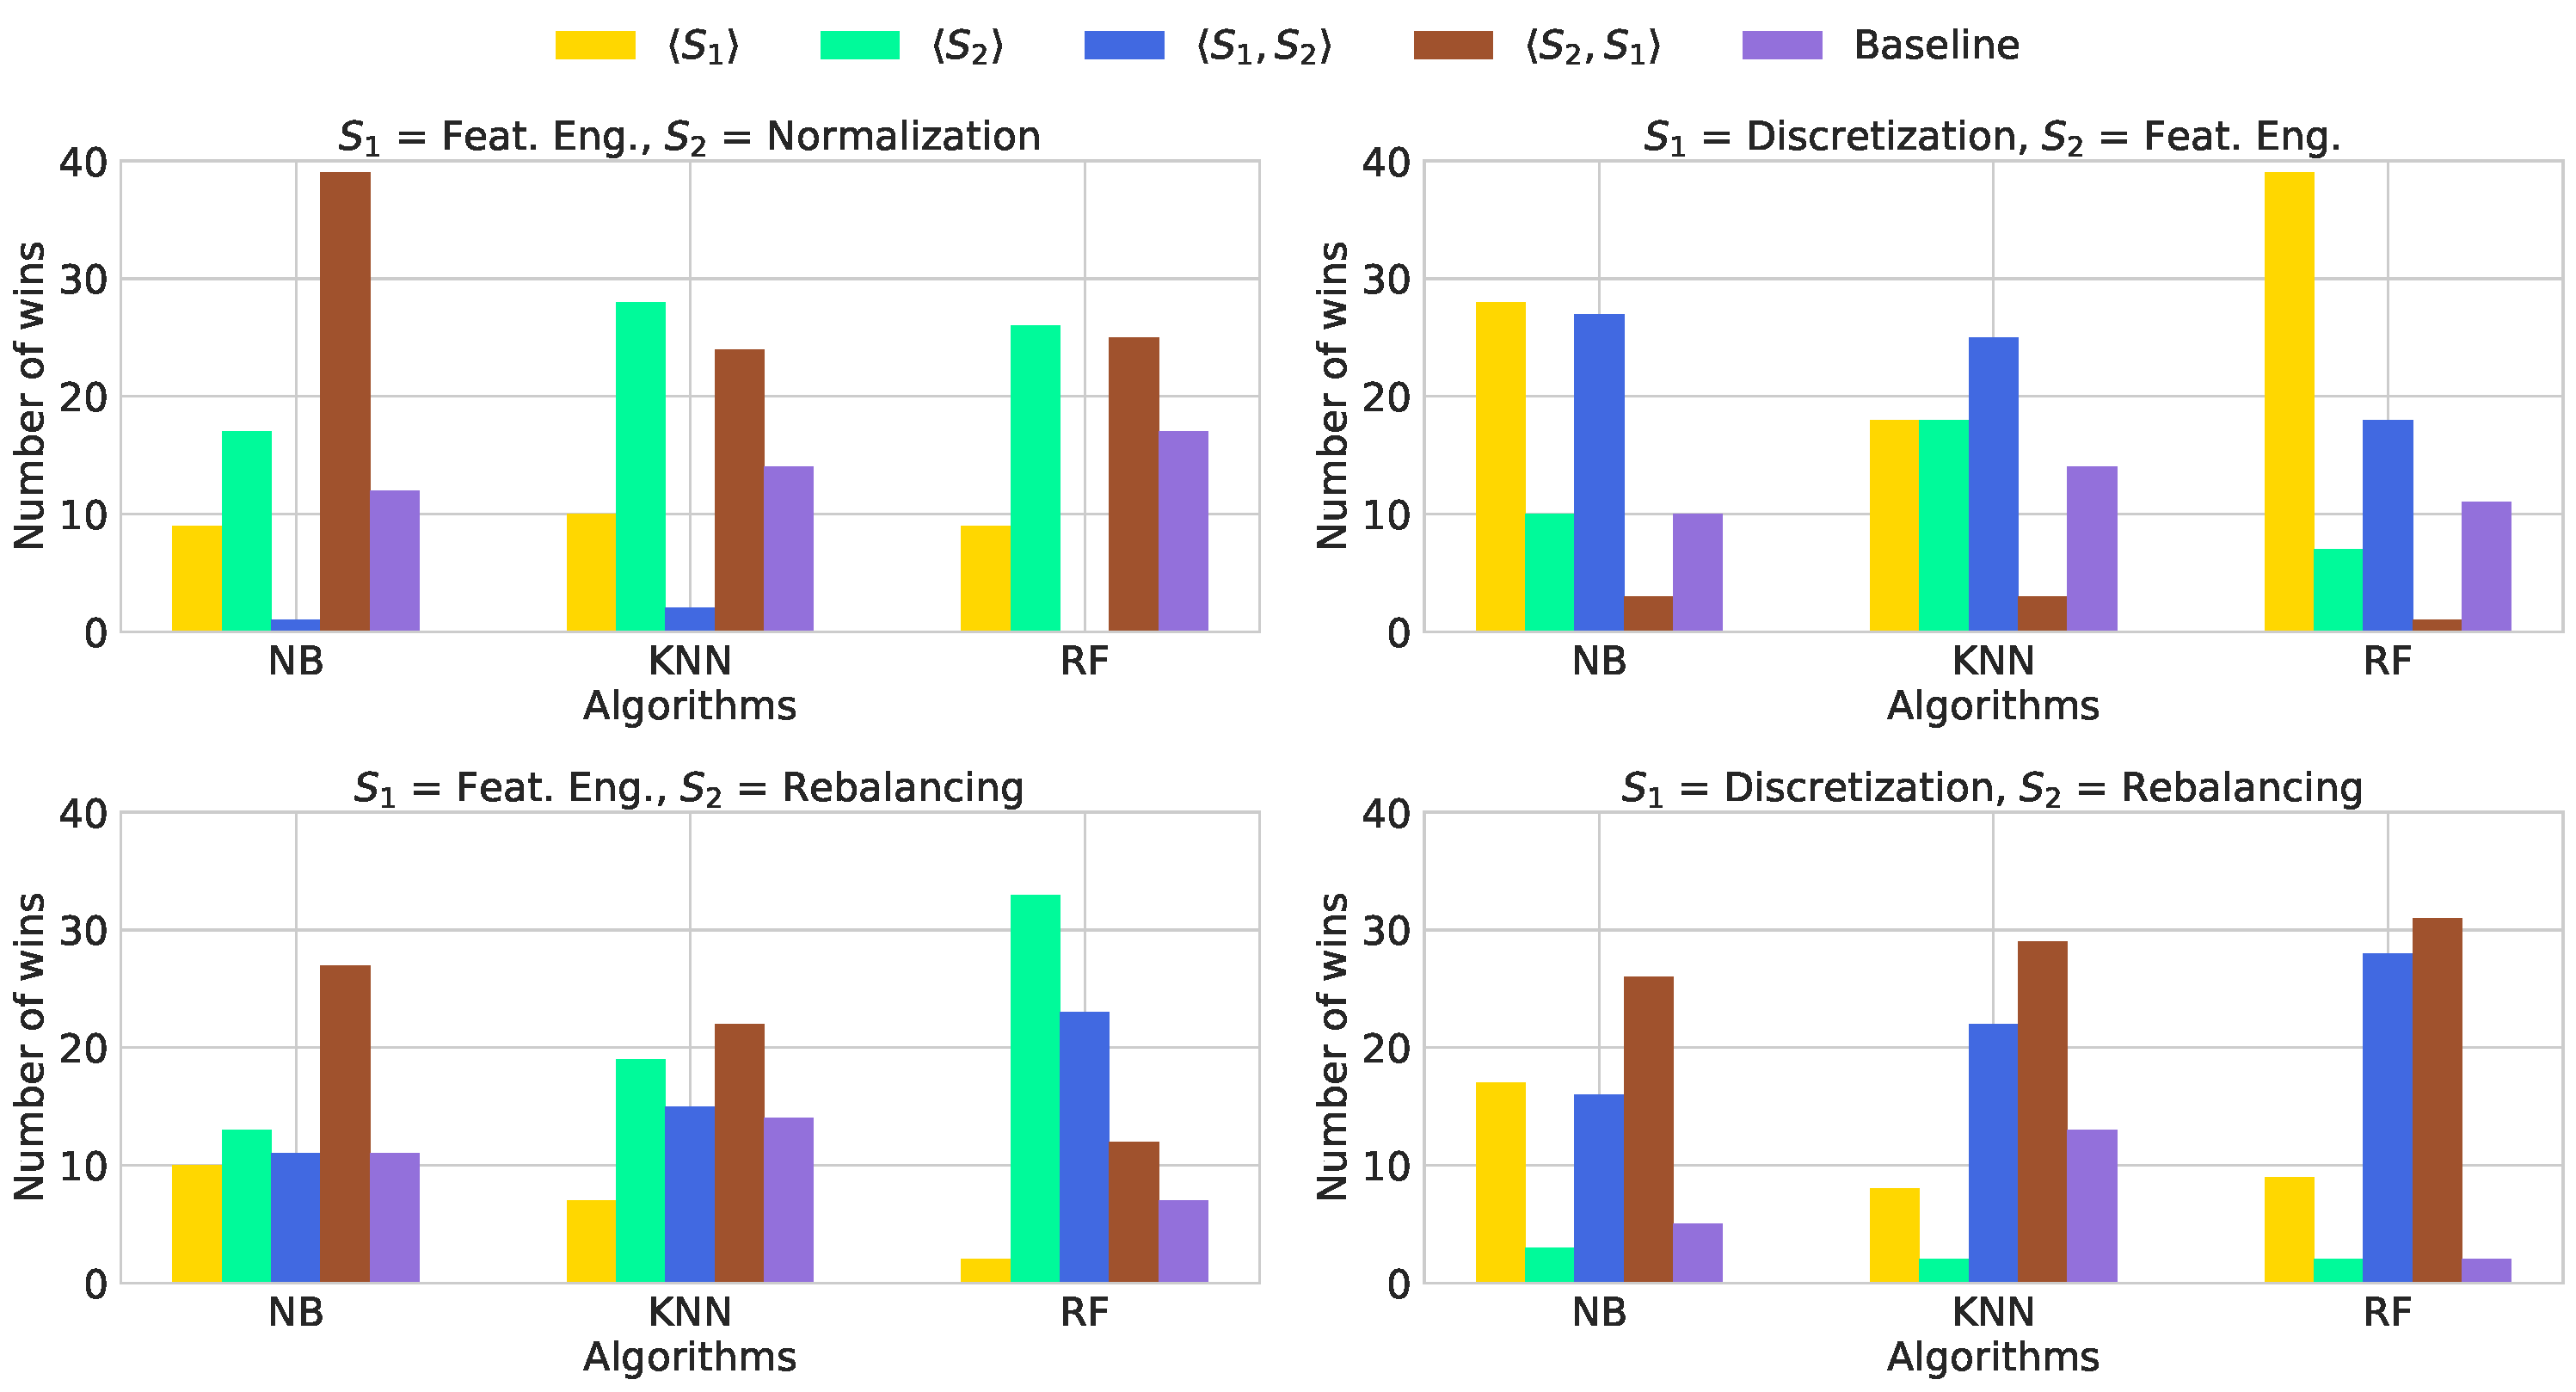
\includegraphics[width=1.0\textwidth]{chapters/data-centric/supervised/img/experiments_results.pdf}
	\caption{Number of datasets for which a given pipeline prototype is declared the winner.}
	\label{effective-fig:learned-rules-results}
\end{figure*}

Applying \Cref{effective-alg:learned-rules}, we obtain a promising order for each pair of transformations considered (i.e., $\{F,N\}$, $\{F,D\}$, $\{F,R\}$, $\{R,D\}$).
Since SMBO is a randomized algorithm, we experimented it with (i) running it several times splitting the budget, and (ii) running it only once with the entire budget.
For the experiments considered, no significant differences where observed, therefore we opted for running it once with the entire budget (i.e., 200 seconds per run), which allows for more configurations to be visited in a single run. Aggregating all the results, \Cref{effective-fig:learned-rules-results} shows the number of datasets, for which a given prototype (\Cref{effective-tbl:validation-rules}, column \textit{winner prototype} for the list of labels) is selected as the winner.
For instance, for the pair $\{F,N\}$ (i.e., Feature Engineering, Normalization), the prototype winning in more datasets for \textit{KNN} and \textit{NB} is $\langle N, F \rangle$.
This means that in general, better results are obtained if Normalization is applied before Feature Engineering.

Next, only $N$ appears as first for \textit{RF} and second best for \textit{KNN} and \textit{NB}, which means that for many datasets, considering different algorithms, it results better to apply only Normalization without combining it with Feature Engineering.
The third position is for $\langle \varnothing, \varnothing \rangle$, which means that for some datasets it is better not to apply any of the steps (in any combination).
The remaining prototypes winning in some datasets are $F$ (only Feature Engineering), and $\langle F, N \rangle$ (Feature Engineering preceding Normalization).
Finally, for three datasets, that are omitted from the figure, there were no winning pipelines (i.e., pipelines resulted in a draw).

Since our goal is to find the best order for a pair of pre-processing steps, we focus on the performances of the pipelines where both of the steps are instantiated (i.e., $\langle S_1, S_2 \rangle$ versus $\langle S_2, S_1 \rangle$).
To do this, we check whether the difference between the number of datasets where they each appear to win is statistically significant by running a binomial test assuming a theoretical probability of $0.5$.
The results are shown in \Cref{effective-tbl:significance-test}.
In summary, the results from \Cref{effective-tbl:significance-test} indicate that, with 95\% confidence we can assume that for the pair $\{F, N\}$, $\langle N, F \rangle$ performs better than $\langle F, N \rangle$, hence Normalization should precede Feature Engineering.
On the other hand, for $\{D, F\}$, $\langle D, F \rangle$ performs better than $\langle F, D \rangle$, hence Discretization should precede Feature Engineering.
Finally, for the remaining transformations, $\{F, R\}$ and $\{R, D\}$, a precedence order can not be pre-assumed since the results obtained are not significant.
Using these results, we create the \textit{Promising precedence} adjacency matrix shown in \Cref{effective-tbl:rules}c, where as one can observe, precedence edges are introduced for $\{N, F\}$ and $\{D, F\}$, but no edges exist neither for $\{F, R\}$, nor for $\{R, D\}$.




\begin{table}[t]
	\centering
	\footnotesize
	\begin{threeparttable}
		\caption{
			Binomial test for determining the order between pairs of transformations. 
		}
		\label{effective-tbl:significance-test}
		\begin{tabular}{@{}cccccc@{}}
			\toprule
			%$S_1$ & $S_2$ & $S_1 \rightarrow S_2$ & $S_2 \rightarrow S_1$ & alpha & \begin{tabular}[c]{@{}c@{}}p-value\\ $H_0:\pi = \pi_0=0.8$\end{tabular} \\ \midrule
			$S_1$ & $S_2$ & $\langle S_1, S_2 \rangle$ & $\langle S_2, S_1 \rangle$ & alpha & p-value\\ \midrule
			$F$ & $N$ & 3 & 88 & 0.05 &  \textbf{0} \\
			$D$ & $F$ & 70 & 7 & 0.05 &  \textbf{0}  \\
			$F$ & $R$ & 49 & 61 & 0.05 & 8.53e-01 \\
			$D$ & $R$ & 66 & 86 & 0.05 & 9.38e-01 \\ \bottomrule
		\end{tabular}
		\begin{tablenotes}
		\centering
		\scriptsize
		\item$N$ - Normalization; $D$ - Discretization; $R$ - Rebalancing; $F$ - Feature Engineering. 
		\end{tablenotes}
	\end{threeparttable}
\end{table}
% \color{black}


\subsubsection{Cross-validation with Chi-square Test}
\label{sec:learned-rules-validation}
After running \Cref{effective-alg:learned-rules} to empirically find a winner between two pairs of transformations, we may obtain a different distribution of the number of wins for the pairs, depending on the datasets considered.
To show that the results obtained with the initial set of datasets are generalizable, we propose to perform an additional cross-validated experiment, where the set of datasets considered can be randomly split into many folds.
Then, for each fold, the results can be compared to the rest, with the aim of checking whether the distributions are similar.
This check can be done via a significance test (e.g., chi-square).
To this end, if the distributions between the folds are similar, it means that the obtained results are independent of the datasets considered, since no matter the combination of the datasets, the results are the same and thus generalizable.

\paragraph{Use case} To show that the results do not depend on the datasests selected, we re-run the experiments (i.e., 10-times each), but this time splitting the datasets into 4-folds.
The goal is to check if the results of the precedence orders from the different folds (i.e., for each experiment considering a randomly different set of datasets) are similar between them (i.e., follow the same distributions).
To confirm this hypothesis, we perform a chi-square test between the results (precedence orders) obtained in a single fold in comparison to the three remaining folds, hence comparing $25$\% of the datasets to the rest.
In particular, to confirm the hypothesis, we need to find results that accept the null hypothesis of the chi-square test which states that ``there is no significant difference between the distributions''.
To do that, sticking to the $95$\% confidence interval, we need to look for p-values greater than $0.05$.
That is, the higher the p-values, the more we accept the null hypothesis, and the more similar the distributions.
Looking at the p-values we found out that they were all much higher than $0.05$.
Specifically, the scores of the chi-square tests of the folds (one fold compared to the rest) are averaged and, after having repeated this procedure 10 times, instead of using a table we depict the 10 averaged p-values using box-plots in \Cref{effective-fig:10-times-4-cv}.
We conclude that, for both of the rules (i.e.,  $\langle F, N \rangle$ and $\langle F, D \rangle$), the significance test indicates a compliance between the new results (\Cref{effective-fig:10-times-4-cv}) and those illustrated above (\Cref{effective-tbl:significance-test}).

\begin{figure*}[!t]
	\centering
	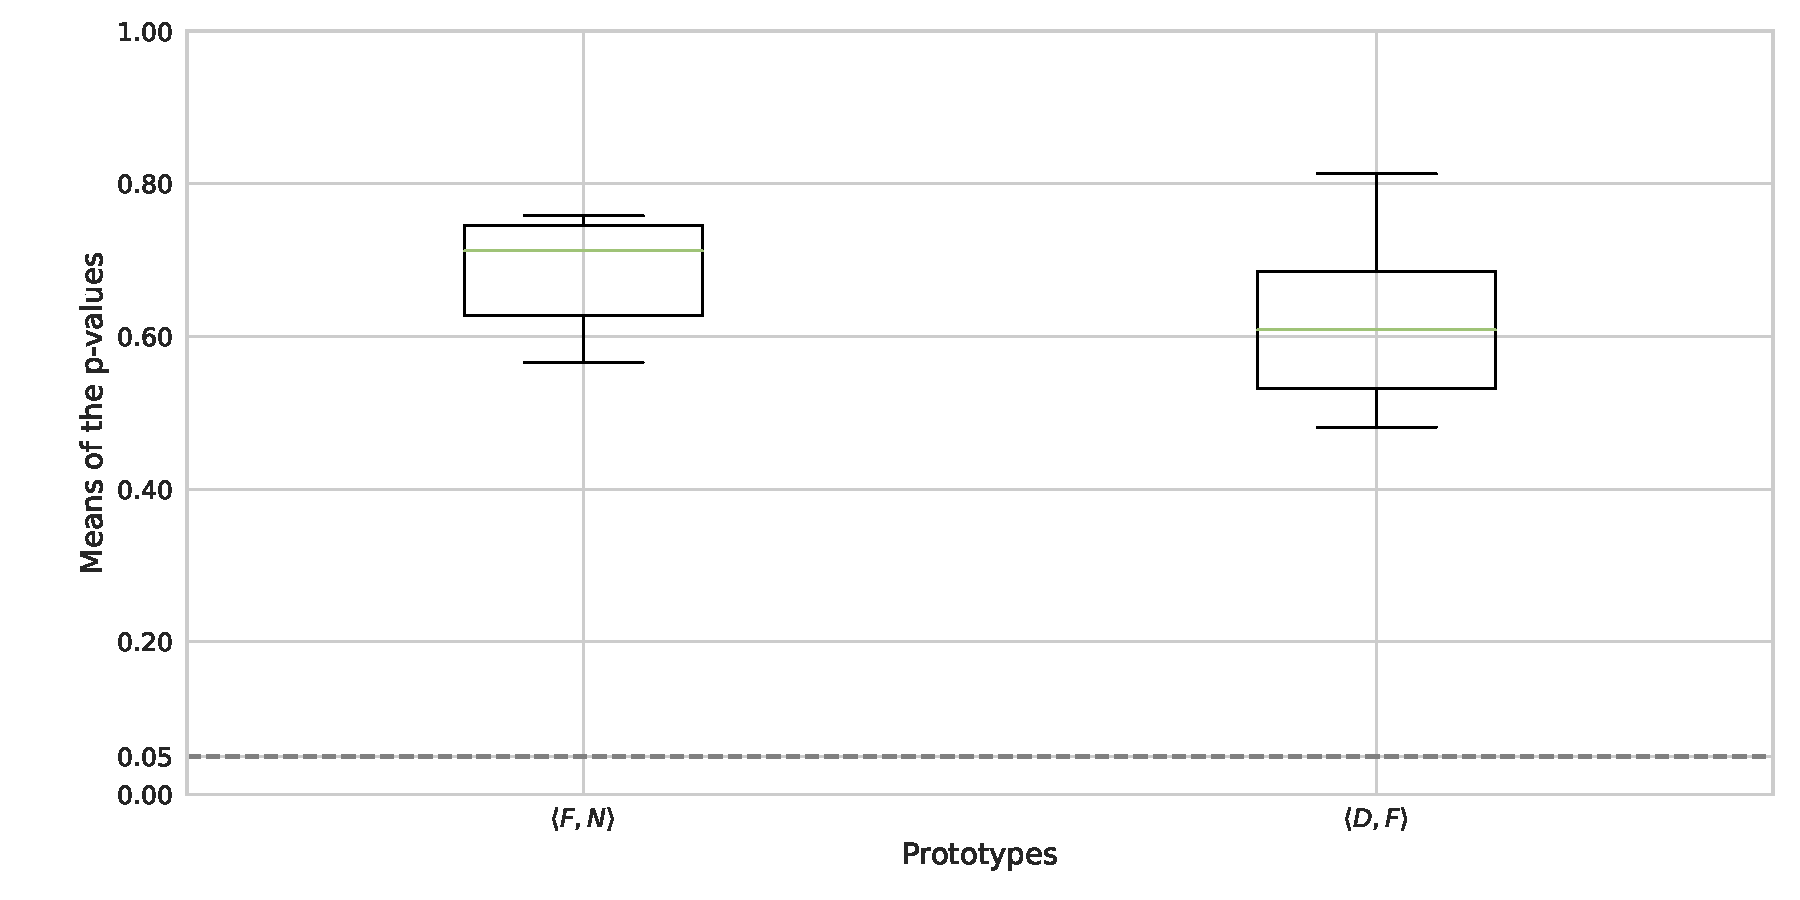
\includegraphics[width=0.9\textwidth]{chapters/data-centric/supervised/img/10_times_4_folds_cv.pdf}
	\caption{The distribution of the p-values obtained after repeating the chi-square test for 10 times, for the 10 times 4-fold cross-validation.}
	\label{effective-fig:10-times-4-cv}
\end{figure*}

\begin{table}[!t]
	\caption{
		Union of rules from \Cref{effective-tbl:rules}.
	}
	\renewcommand{\arraystretch}{0.3}
	\footnotesize
	\centering
	\label{effective-tbl:rules-union}
	\begin{threeparttable}
		\begin{tabular}{p{1cm}p{1cm}p{1cm}p{1cm}p{1cm}p{1cm}p{1cm}}
			\toprule
			& $\boldsymbol{E}$ & $\boldsymbol{N}$ & $\boldsymbol{D}$ & $\boldsymbol{I}$ & $\boldsymbol{R}$ & $\boldsymbol{F}$
			\\	\cmidrule[.1em]{1-7}
			$\boldsymbol{E}$ & \cellcolor{gray!25} & \texttt{1} & \texttt{1} & \texttt{0} & \texttt{1} & \texttt{1} \\	\cmidrule[.1em]{1-7}
			$\boldsymbol{N}$ & \texttt{0} & \cellcolor{gray!25}  & \texttt{X} & \texttt{0} & \texttt{1} & \texttt{1} \\	\cmidrule[.1em]{1-7}
			$\boldsymbol{D}$ & \texttt{0} & \texttt{X} & \cellcolor{gray!25} & \texttt{0} & \texttt{0} & \texttt{1} \\	\cmidrule[.1em]{1-7}
			$\boldsymbol{I}$ & \texttt{1} & \texttt{1} & \texttt{1} & \cellcolor{gray!25}  & \texttt{1} & \texttt{1} \\	\cmidrule[.1em]{1-7}
			$\boldsymbol{R}$ & \texttt{0} & \texttt{0} & \texttt{0} & \texttt{0} & \cellcolor{gray!25}  & \texttt{0} \\	\cmidrule[.1em]{1-7}
			$\boldsymbol{F}$ & \texttt{0} & \texttt{0} & \texttt{0} & \texttt{0} & \texttt{0} & \cellcolor{gray!25} \\	\cmidrule[.1em]{1-7}
		\end{tabular}
		\begin{tablenotes}
			\scriptsize
			\item$\boldsymbol{E}$ - Encoding; $\boldsymbol{N}$ - Normalization; $\boldsymbol{D}$ - Discretization; $\boldsymbol{I}$ - Imputation; $\boldsymbol{R}$ - Rebalancing; $\boldsymbol{F}$ - Feature Engineering. \item \texttt{1} - a precedence edge exists between the row and the column, \texttt{0} - a precedence edge does not exist between the row and the column, \texttt{X} - the combination is meaningless.
		\end{tablenotes}
	\end{threeparttable}
\end{table}

\subsection{Effective Prototypes Composition}
\label{effective-ssec:composition}

In this, we foresee the composition of the previously defined rules (i.e., for the pairs of pre-processing steps), to generate the final set of rules that would allow to compose longer chains---consisting of more than two steps.
This is when we also resolve the inconsistencies and define precedences for the pairs of steps that may not have any precedence defined already---in that case, we basically take into account all the permutations.
This allows to finally generate the possible effective  prototypes.

\paragraph{Use case}
To generate the final prototypes, in this phase, we combine all the matrices generated by the previous steps.
That is, we take the union of the edges (represented by \texttt{1}'s) from the matrices in \Cref{effective-tbl:rules} (a,b,c), and create a new final adjacency matrix, shown in \Cref{effective-tbl:rules-union}.
This is the matrix that will allow us to generate the final effective prototypes.

Observing the table, one can realize that for pairs $\{F,R\}$ and $\{R,D\}$, no precedence edges exist.
This means that these pairs are somewhat equally relevant from either direction (any order), and thus when generating the final prototypes, both options should appear.

For a better reading, in Figure~3.6, we visualize \Cref{effective-tbl:rules-union} in form of a graph, where nodes represent the pre-processing steps and the directed edges represent a precedence order between them.
Out of the graph, we generate the final prototypes by taking all the maximum length variations (ordered arrangements without repetition) of the nodes, respecting the precedence rules (i.e., not contradicting the direction of existing edges).
The result is the set of five prototypes shown in Table 3.7. This set consisting of \textit{compatible}, \textit{meaningful} and \textit{promising} pairs of transformations is the set of recommended \textit{effective pipeline prototypes}.


\begin{figure}
	\begin{floatrow}
	\ffigbox{
		\includegraphics[clip, trim=2.5cm 23cm 10.5cm 2cm,width=0.5\textwidth]{chapters/data-centric/supervised/img/graph.pdf}
	}{
		  \caption{Precedence graph generated from \Cref{effective-tbl:rules-union}.}
	}
	\capbtabbox{
	\begin{tabular}{@{}ll}
				\toprule
				ID& Pipeline prototype                                             \\ \toprule
				1&{\color[HTML]{000000} $\langle I, E, N, R, F  \rangle$} \\
				2&{\color[HTML]{000000} $\langle I, E, N, F, R \rangle$} \\
				3&{\color[HTML]{000000} $\langle I, E, R, D, F \rangle$} \\
				4&{\color[HTML]{000000} $\langle I, E, D, R, F \rangle$} \\
				5&{\color[HTML]{000000} $\langle I, E, D , F, R \rangle$} \\
				\bottomrule
			\end{tabular}
	}{
		  \caption{Effective prototypes generated from Figure~3.6.
		}
	}
	\end{floatrow}
\end{figure}

\subsection{Meta-learning of Instantiation Rules}
\label{effective-ssec:meta-learning}

Once the pipeline prototypes are constructed (i.e., the order between the steps is defined), what follows is their instantiation with the actual transformations.
For that, one can rely completely on SMBO, and let the optimization choose the right transformation for each step.
However, as many optimization techniques, SMBO suffers from the cold-start problem where, in the beginning, it does not have enough information to come up with promising configurations, and a wrong choice may affect the whole process.

\subsubsection{Exploratory Analysis}
Given the availability of the experimental SMBO executions (executed in an exhaustive manner, considering all the prototypes), one can perform an exploratory analysis with the aim of removing useless prototypes, executable pipelines or sngle transformations.
Hence, further tweaking the search space.
In particular, one might analyze whether:

\begin{itemize}
    \item there exist some combination of steps (\Cref{effective-tbl:pipeline-enumeration}), that are generally useless (i.e., in terms of their impact on the final performance), and thus can be discarded a priori to reduce the search space;
    \item there are some executable pipelines that are consistently chosen more often than others by the optimization, meaning that they are more useful than others;
    \item within the executable pipelines, some transformations are chosen more often than others, meaning that they provide a more positive impact.
    \end{itemize}

\paragraph{Use case}
We performed the above-mentioned analysis, but this did not lead to any conclusive or significant results.
In particular, as shown in \Cref{effective-fig:prototypes-impact}, we could not find any useless prototypes---not positively impacting the final accuracy, that could be discarded a priori from the potential list of prototypes.
Actually, as we will show in \Cref{effective-sec:eval-universal-pipeline}, all of them lead to the best in one case or another, which does not mean the epsilon improvement some provide is worth the search cost you incur in considering them (but this more in-depth analysis is done later).
Next, as shown in \Cref{effective-fig:pipeline-frequency}, there were no physical pipelines shown to be more useful---hence more often selected, than others.
Even if $\langle N , R \rangle$ is clearly above, it barely reaches 30\% in KNN.
Finally, observing \Cref{effective-fig:transformation-frequency}, it is clear that some kinds of transformations are chosen more often, but looking closely (i.e., the shaded bars), it is not clear which operator brings more benefit.
For instance, Normalization is present in 90\% of the pipelines, but it is not easy to distinguish which kind of Normalization (i.e., actual operator) is more beneficial.
For this, we need more complex rules or guidelines that may help in finding the right operator to use.


\begin{figure*}[!t]
	\centering
	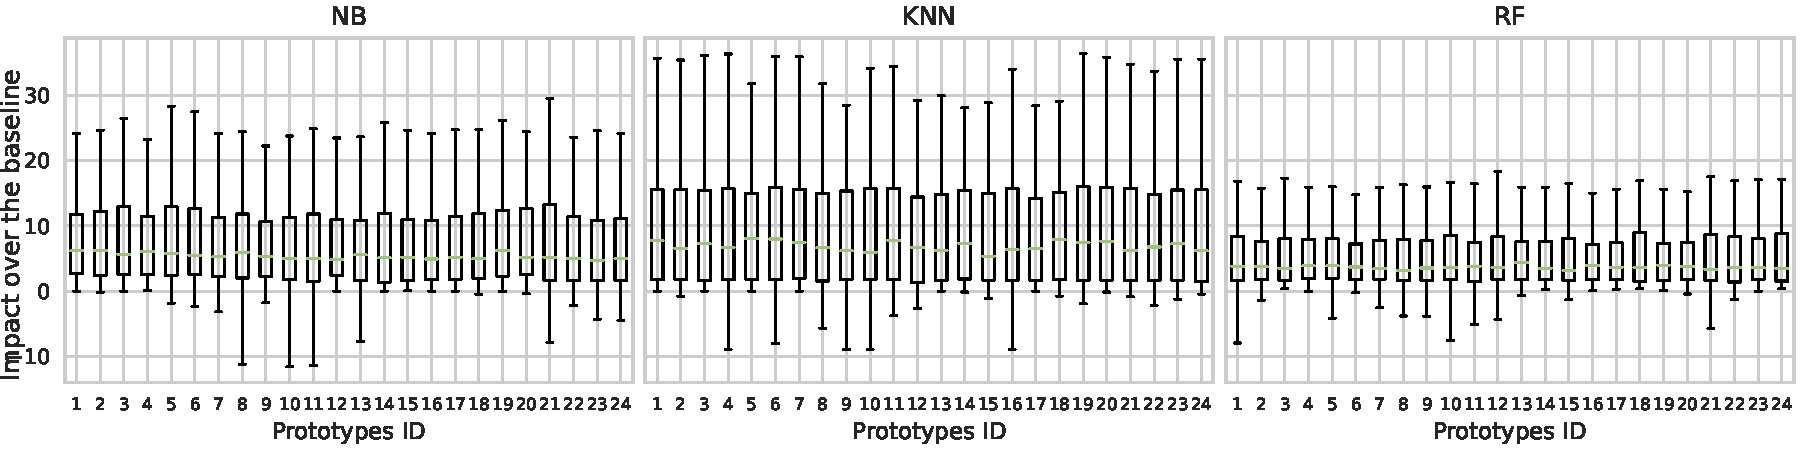
\includegraphics[width=1.0\textwidth]{chapters/data-centric/supervised/img/prototypes_impact.pdf}
	\caption{The impact of the different pipeline prototypes over the baseline (i.e., when no transformation is applied).}
	\label{effective-fig:prototypes-impact}
\end{figure*}

\begin{figure*}[!h]
	\centering
	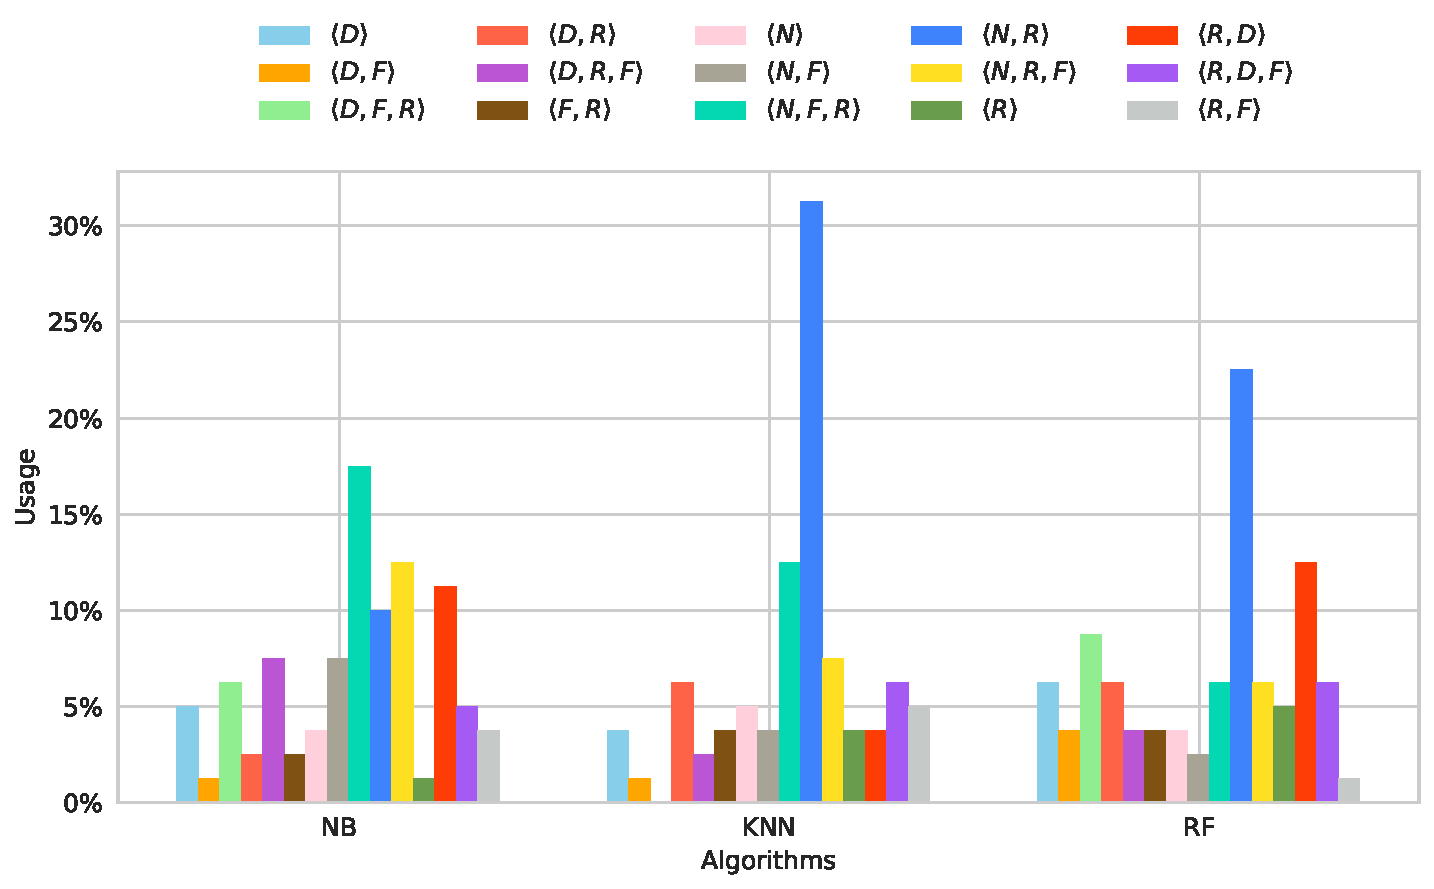
\includegraphics[width=1.0\textwidth]{chapters/data-centric/supervised/img/pp_pipeline_study2.pdf}
	\caption{Percentage of use of the different physical pipelines.}
	\label{effective-fig:pipeline-frequency}
\end{figure*}

\begin{figure*}[!h]
	\centering
	\includegraphics[width=0.7\textwidth]{chapters/data-centric/supervised/img/pp_pipeline_study_grouped.pdf}
	\caption{Percentage of use of a transformation in a physical pipeline.}
	\label{effective-fig:transformation-frequency}
\end{figure*}

\subsubsection{Meta-learning}
To mitigate the cold-start problem, we propose to perform meta-learning, where we intend to use the knowledge extracted from historical data in order to devise rules that may help the optimization in its initial settings.
Meta-learning is the process of ``learning on top of learning'', or learning a model using historical data from ML experiments.
Traditionally, it has been used for predicting the performance (e.g., accuracy) of an algorithm on a given dataset.
That is, given some historical runs of the performance of classification algorithms over various datasets (i.e., meta-dataset: consisting of datasets characteristics as meta-features and the performance of the ML algorithm as the desired outcome in a regression task), one can learn a model (i.e., meta-model), that is able to predict the performance of a given ML algorithm on a new dataset \cite{Brazdil04Book}.
Lately, this technique has been extended in order to predict the impact of pre-processing steps over the performance of ML algorithms and thus rank them based on the impact \cite{Bilalli17AMCS, presistant18CSI, presistant19DKE}.
The same idea can be applied to learning the best trnasformation for a given step.
That is, through meta-learning one can learn the intrinsic relationship between dataset characteristics and the transformation performance, and thus come up with rules that are not obvious and are effective at the time of pipeline instantiation.
The main idea is to build a model, that is able to predict the transformation for a certain pre-processing step, given the meta-features extracted from the dataset considered for the optimization.
This translates to answering the following question: ``given that we know the dataset characteristics and having selected a certain pre-processing step (e.g., Imputation), what is the optimal transformation we need to obtain the highest improvement w.r.t. loss (i.e., when the ML algorithm is applied over the transformed dataset)?''.
In particular, the model can generate a set of complementary rules that help in the optimization, providing a good starting instantiation for some of the steps in the prototype.

To train the model we need a meta-dataset that can be  (i) generated through optimization algorithms (e.g., SMBO executions), (ii) generated manually through simple evaluations of classification algorithms over transformed datasets, or (iii) assumed already given (e.g., OpenML).
Given a meta-dataset, we propose to learn to predict the best instantiation (transformation) for a given pre-processing step, including skipping the step (class \texttt{None}).

\paragraph{Use case}
Our training dataset for the meta-learning (i.e., meta-dataset) is built through SMBO runs on the OpenML datasets (\Cref{effective-ssec:rules-learned}).
We first extract the dataset characteristics (i.e., meta-features; e.g., number of features, number of instances, number of missing values).
Then, by applying SMBO optimization on classification algorithms and pre-processing prototypes, for each dataset, we retrieve the loss (in our case, accuracy) of the ML algorithms over the optimized pipelines.
This gives us the optimized executable pipelines and their impact on the accuracy of the learning algorithms for each dataset at hand.
Given such information, our aim is to now save time and improve the instantiation of the transformations for each step considered in the prototype.

We trained several different conditional inference trees (i.e., a particular implementation of decision trees \cite{ctree}) because they produce models that can be easily read and interpreted.
Specifically, the independence of each meta-feature with the class (transformation of a specific step) is tested through a statistical test.
The split is made on the variable with the lowest p-value.
We report the p-value too so that it can be seen how strong the association is (i.e., why that variable was chosen).
We stick with the p-value threshold of $0.05$, and devise a rule from any branch of the tree that is within the threshold.
In the following, we describe the rules obtained within the selected significance threshold.


\begin{figure}[!h]
	\centering
	\includegraphics[clip, trim=1.0cm 0.4cm 1cm 1cm,width=1\textwidth]{chapters/data-centric/supervised/img/tree-FE.pdf}
	\caption{Conditional Inference Tree built for the \textit{Features Engineering} transformation.}
	\label{effective-fig:features-meta-learning:feature-engineering}
\end{figure}

\textbf{Rules for Feature Engineering}. The available transformations in scikit-learn for Feature Engineering are: Principal Component Analysis (\texttt{PCA}), \texttt{Feature Selection} (Select K Best), \texttt{Both} (PCA + Select K Best), and \texttt{None}.
The tree generated for the Feature Engineering transformation is shown in \Cref{effective-fig:features-meta-learning:feature-engineering}.
The leaves show the selected transformation frequency.
For the sake of simplicity, we do not consider the union of PCA and Select K Best as a transformation per se, instead we distribute that contribution to the two operators that compose it.
Observe that there is a strong correlation between the Feature Engineering transformation and the entropy of the class.
Indeed, such a meta-feature achieved a p-value smaller than $0.001$.
We can clearly read that if the Class Entropy is low, then \texttt{Feature Selection} is way more chosen than the other options (see Node 2).
Recall that entropy is a measure of how much disorder there is in its domain.
The less is that value, the easier is the classification problem.
As a consequence, it is reasonable to think that the easier the classification problem is, the more likely is the fact that the class can be described by a low number of features.
Hence, the \texttt{Feature Selection} technique can be successfully applied.
Conversely, Node 5 shows that, when the Class Entropy is high, it is better to not apply any Feature Engineering operator.
As a matter of fact, a high value of Class Entropy involves a high number of classes and/or few instances per class, hence a really difficult problem.
In such cases, reducing the dimensionality of the dataset does not lead to any improvement.
Finally, when the Class Entropy is in between, there is no clear winner, and thus other non-obvious factors may affect the choice of the operator.

\begin{figure}[!h]
	\centering
	\includegraphics[clip, trim=5.8cm 0.4cm 5.05cm 3.5cm,width=0.65\textwidth]{chapters/data-centric/supervised/img/tree-RE.pdf}
	\caption{Conditional Inference Tree built for the \textit{Rebalancing} transformation.}
	\label{effective-fig:features-meta-learning:rebalancing}
\end{figure}

\textbf{Rules for Rebalancing}. As for Rebalancing, the transformations considered from the imblearn\footnote{\url{https://pypi.org/project/imbalanced-learn}} library are: \texttt{Near Miss}, \texttt{SMOTE}, and \texttt{None}.
The first is an undersampling algorithm which randomly eliminates the samples from the larger class; the second is an oversampling technique that creates samples of the minority class, as a linear combination of them.
As shown in \Cref{effective-fig:features-meta-learning:rebalancing}, the meta-feature Majority Class Percentage has a p-value of $0.014$.
This can be read as, in case of an unbalanced class problem (i.e., Node 3: Majority Class Percentage greater than 56), an oversampling of the minority class(es) is preferred to a downsampling of the majority one(s).
However, when the Majority Class Percentage is smaller than 56\%, the situation is not that clear, and there is no technique that is applied significantly more often than the rest; they are close to each other.
Therefore, it is difficult to understand which problems (which dataset characteristics do they have) belong to Node 2.
In summary, when the majority class has no more than 56\% , it implies that it is an unbalanced class, and as mentioned above, SMBO tends to choose the same transformation.
However, when the majority class has less than 56\%, it may imply that: (i) there are just two classes and the problem counts as a balanced problem, so no transformation needs to be applied, or (ii) it is a multi-class problem, and thus there is no clear winner in terms of transformation.

\subsection{Data Pipeline Instantiation}
\label{effective-ssec:prototype-insta}

The prototypes from the top flow and the meta-lerning rules from the bottom flow (if the optimization framework permits) are finally fed to the final phase which deals with the instantiation and optimization of the prototypes. In this, we run SMBO until an optimized pipeline is found.

\paragraph{Use case}
 In our final execution, we run SMBO to find a suitable instantiation for the suggested prototypes. The simple but not obvious meta-learning rules, even though not included in our final execution, because of the implementation considered (i.e., HyperOpt), can potentially be used to ease the cold-start problem.

\section{Empirical Evaluation}
\label{effective-sec:evaluation}


The aim of our experimental study is three-fold:
\begin{enumerate}
    \item Check whether there exists a universal prototype that works best for any classification problem considered  (i.e., dataset and ML algorithm) (\Cref{effective-sec:eval-universal-pipeline}).
    \item Assess and compare the performance of optimizing the effective prototypes constructed using our method against the set of exhaustively generated prototypes (\Cref{effective-sec:eval-our-vs-rest}).
    \item Assess and compare the impact of dedicating a portion of the optimization time to the effective prototypes against using the whole optimization time for the hyperparameters of the ML algorithm (\Cref{effective-sec:eval-dpso-vs-cash}).
\end{enumerate}

The experiments were performed on an Intel Core i7 machine with 12 cores, running at 3.20 GHz with 64 GB of main memory.
We leveraged the SMBO optimization algorithm available in the Python library HyperOpt \cite{bergstra2015hyperopt}.
The datasets used in the experiments are the ones from the OpenML CC-18 repository \cite{OpenML2013}.
Finally, the classification algorithms considered are \textit{NB}, \textit{KNN}, and \textit{RF} from the Python library Scikit-learn \cite{scikit-learn}.
All the experiments for a single algorithm took approximately two weeks.


\paragraph{AutoPrep}
With the recent shift towards data-centric approaches, rather than algorithmic, data pre-processing is receiving a lot of attention.
Yet, its impact on the final analysis is not widely recognized, primarily due to the lack of publicly available experiments that quantify it.
To bridge this gap, along with this work, we contribute to publishing a companion reproducibility paper \cite{Giovanelli2022IS} for the experiments and results reported in the following.
AutoPrep introduces a set of reproducible experiments on the impact of data pre-processing by providing a detailed reproducibility protocol together with a software tool and a set of extensible datasets, which allow for all the experiments and results of this chapter reproduced.
Our experiments have been performed among different machines with different resources.
We achieved to deploy \textit{strongly reproducible experiments}, when based on a collection of intermediate results, and \textit{weakly reproducible experiments} when reproducing our end-to-end optimization from scratch.
The reproducibility protocol is created in Docker and tested in Windows and Linux.
The source code and the datasets for reproducing the experiments can be found on GitHub\footnote{
\url{https://github.com/josephgiovanelli/autoprep}}.

\begin{definition}[Strongly reproducible experiment  \cite{reproducible}]
    \label{def:strong}
    Given a set of previously reported experimental results and conclusions, a computational experiment is strongly reproducible if it allows to confirm both previously reported results and conclusions exactly.
\end{definition}

\begin{definition}[Weakly reproducible experiment  \cite{reproducible}]
    \label{def:weak}
    Given a set of previously reported experimental results and conclusions, a computational experiment is weakly reproducible if the Spearman rank correlation between the original and reproduced results is equal to 1, and their Pearson correlation value is high enough to allow the confirmation of all previously reported conclusions, even if the reproduced results do not reproduce all results exactly. Thus, weak reproducibility is a performance-rank-preserving notion.
\end{definition}

\subsection{Universal Pipeline Prototype}
\label{effective-sec:eval-universal-pipeline}
The goal of this experiment is to demonstrate the difficulty of blindly finding the right prototype (i.e., without considering any meaningful or promising precedence).
In \Cref{effective-tbl:pipeline-enumeration}, we list the exhaustive set of pipeline prototypes generated considering the compatible precedence graph in Table~\ref{effective-tbl:rules}a (i.e., 24 compatible permutations).
In a real scenario, this number would be too high for splitting the time budget in order to optimize them.
Yet, for the sake of this experiment, we exhaustively optimize all the prototypes, for each dataset.
Thus, for each prototype and for each dataset, the SMBO algorithm is configured to assign a 200 seconds time budget to the phase of instantiating and optimizing the prototype, and another 200 seconds to the phase of optimizing the hyperparameters of the ML algorithm.

\begin{table}[t]
\caption[Enumeration of the prototypes that can be generated by compatible precedence]{Exhaustive set of prototypes generated using the compatible precedence graph of Table~\ref{effective-tbl:rules}a. $E$ - Encoding; $N$ - Normalization; $D$ - Discretization; $I$ - Imputation; $R$ - Rebalancing; $F$ - Feature Engineering.
}
\footnotesize
\label{effective-tbl:pipeline-enumeration}
\begin{center}
\begin{tabular}{@{}lllll@{}}
\toprule
ID & Pipeline prototype & ID & Pipeline prototype                                                                   \\ \toprule
1  & {\color[HTML]{000000} $\langle I, E, N, D, F, R \rangle$} & 13 & {\color[HTML]{000000} $\langle I, E, F, N, D, R \rangle$} \\
2  & {\color[HTML]{000000} $\langle I, E, N, D, R, F \rangle$} & 14 & {\color[HTML]{000000} $\langle I, E, F, N, R, D \rangle$} \\
3  & {\color[HTML]{000000} $\langle I, E, N, F, D, R \rangle$} & 15 & {\color[HTML]{000000} $\langle I, E, F, D, N, R \rangle$} \\
4  & {\color[HTML]{000000} $\langle I, E, N, F, R, D \rangle$} & 16 & {\color[HTML]{000000} $\langle I, E, F, D, R, N \rangle$} \\
5  & {\color[HTML]{000000} $\langle I, E, N, R, D, F \rangle$} & 17 & {\color[HTML]{000000} $\langle I, E, F, R, N, D \rangle$} \\
6  & {\color[HTML]{000000} $\langle I, E, N, R, F, D \rangle$} & 18 & {\color[HTML]{000000} $\langle I, E, F, R, D, N \rangle$} \\
7  & {\color[HTML]{000000} $\langle I, E, D, N, F, R \rangle$} & 19 & {\color[HTML]{000000} $\langle I, E, R, N, D, F \rangle$} \\
8  & {\color[HTML]{000000} $\langle I, E, D, N, R, F \rangle$} & 20 & {\color[HTML]{000000} $\langle I, E, R, N, F, D \rangle$} \\
9  & {\color[HTML]{000000} $\langle I, E, D, F, N, R \rangle$} & 21 & {\color[HTML]{000000} $\langle I, E, R, D, N, F \rangle$} \\
10 & {\color[HTML]{000000} $\langle I, E, D, F, R, N \rangle$} & 23 & {\color[HTML]{000000} $\langle I, E, R, D, F, N \rangle$} \\
11 & {\color[HTML]{000000} $\langle I, E, D, R, N, F \rangle$} & 23 & {\color[HTML]{000000} $\langle I, E, R, F, N, D \rangle$} \\
12 & {\color[HTML]{000000} $\langle I, E, D, R, F, N \rangle$} & 24 & {\color[HTML]{000000} $\langle I, E, R, F, D, N \rangle$}
\\ \bottomrule
\end{tabular}
\end{center}
\end{table}

The results obtained are shown in \Cref{effective-fig:eval-universal-pipeline}.
The enumerated prototypes are listed in the abscissa axis and each stacked bar represents the percentage of cases for which that prototype achieved the best performance across different ML algorithms (the contribution of each algorithm is represented with a different color).
In an ideal scenario, for a prototype to be considered \textit{universal}, it should perform best in all or at least most of the cases, which is clearly not happening.
Observe that, even the best-performing prototype is only the best in 19\% of the cases, which is obviously far from being \textit{universal}.
Hence all (or at least several) prototypes need to be evaluated together, in order to obtain better solutions.

\begin{figure}[t]
    \centering
    \includegraphics[width=0.8\textwidth]{chapters/data-centric/supervised/img/evaluation1.pdf}
    \caption{Comparison of the goodness of the exhaustive set of prototypes.}
    \label{effective-fig:eval-universal-pipeline}
\end{figure}

\subsection{Exhaustive Versus Effective Prototypes}
\label{effective-sec:eval-our-vs-rest}
Given that there is no single universal prototype, one can opt for feeding all the possible prototypes (see \Cref{effective-tbl:pipeline-enumeration}) to the optimization algorithm in order to get the best solutions out of them.
As before, we assign a budget of 200 seconds for the optimization of each prototype, hence 80 minutes in total for all the set of 24 \textit{exhaustive prototypes} in order to find the optimal pipeline for every dataset.
On the other hand, we take only the five \textit{effective prototypes} resulting from the application of our method and assign just 40 seconds time budget for the optimization of each one of them, hence 200 seconds in total. With the aim of comparing the two, and thus roughly understanding how close we are to the optimal case, in both cases, we dedicated the same time budget (i.e., 200 seconds) for the phase of optimizing the hyperparameters of the ML algorithm.
In order to evaluate how close the \textit{effective prototypes} are to the \textit{exhaustive ones}, we calculate the \textit{normalized distance} from the result to the optimum---w.r.t. accuracy.

\begin{equation*}
    normalized\;distance = \frac{ACC_{\textup{eff}} - ACC_{\varnothing}}{ACC_{\textup{exh}} - ACC_{\varnothing}}
\end{equation*}

$ACC_{\varnothing}$ is the baseline performance (i.e., accuracy of the algorithm $A$ with default hyperparameters and no data pipeline, hence computed over the original dataset $\altmathcal{D}$), formally $ACC_{\varnothing} = ACC( \langle \varnothing, A  \rangle (\altmathcal{D}_{train}), \altmathcal{D}_{valid})$.
$ACC_{\textup{eff}}$ is the accuracy of the optimized algorithm $A_{{\lambda}^{\star}}$ over the dataset transformed using the optimized instantiation of the effective set of prototypes (i.e., our approach), formally $ACC_{\textup{eff}} = ACC(\langle P^{\star}_{\textup{eff}_{{\lambda}^{\star}}}, A_{\lambda^\star} \rangle (\altmathcal{D}_{train}), \altmathcal{D}_{valid})$.
Finally, $ACC_{\textup{exh}}$ is the accuracy of the optimized algorithm $A_{{\lambda}^{\star}}$ over the dataset transformed using the optimized pipeline instantiation of the exhaustive set of prototypes, formally $ACC_{\textup{exh}} = ACC(\langle P^{\star}_{\textup{exh}_{{\lambda}^{\star}}}, A_{\lambda^\star} \rangle (\altmathcal{D}_{train}), \altmathcal{D}_{valid})$.
The subtraction by $ACC_{\varnothing}$ is done with the aim of weighting the difficulty of a dataset, hence allowing for comparisons in terms of the gain in accuracy.
To this end, the bigger the potential gain (denominator) is, the bigger the obtained gain (numerator) must be, for the latter to be relevant.

The results obtained for every dataset and algorithm are shown as boxplots in \Cref{effective-fig:eval-exhaustive-vs-effective}.
Observe that, most of the cases are very close to the results obtained using the exhaustive set, the median distances being 91.51\%, 93.13\%, 88.97\%, for NB, KNN, and RF, respectively.
In general, in 75\% of the cases the chosen pipelines are above 80\%, and only few outliers are below 60\%.
Curiously, in some cases, we outperform the results over the exhaustive set of pipelines, but this is due to the randomness of the optimization algorithm, which unless it is given an unrealistically high budget of time, is not capable of finding the true optimal solution.
We discarded the option of assigning a larger budget since this was not practical considering the huge search space and the lack of any guarantee of improvement.

To summarize, the experiment shows that with roughly 24 times less time budget, we can obtain results that are as good as 90\% in the median compared to the exhaustive ones.
The raw results (i.e., without the normalized distances) can be found on the aforementioned GitHub page.

\begin{figure}[!t]
    \centering
    \includegraphics[width=1.0\textwidth]{chapters/data-centric/supervised/img/evaluation2.pdf}
    \caption{Normalized distances between the scores obtained by optimizing our effective prototypes and the ones obtained by optimizing the exhaustive set.}
    \label{effective-fig:eval-exhaustive-vs-effective}
\end{figure}

\subsection{Complementing HPO of ML algorithm with Pre-processing}
\label{effective-sec:eval-dpso-vs-cash}

\begin{figure*}[!t]
	\centering
	\includegraphics[width=1.0\textwidth]{chapters/data-centric/supervised/img/barplot-10.pdf}
	\caption{The impact of dedicating a portion of the optimization budget to pre-processing compared to using the whole optimization budget for the ML algorithm HPO.}
	\label{effective-fig:eval-pre-processing-hyperparameter}
\end{figure*}

We have just shown that our effective prototypes have similar impact as the exhaustive ones.
Now we want to compare the impact of the effective prototypes against optimizing only the hyperparameters of the ML algorithm.
That is, we want to examine whether dedicating a part of the optimization budget to the pre-processing impacts more (positively) the results of the analysis, than using the whole budget for solely the hyperparameter optimization of the ML algorithm\footnote{To enable the application of the ML algorithms on all the datasets, whenever required, we apply the necessary transformation (e.g, imputation or encoding).}---i.e., modelling.

To this end, for the latter we now dedicate the total optimization budget (i.e., 400 seconds), and for the former, inspired by \cite{Quemy20InfSystems}, we split the budget 50-50 between the pre-processing pipeline optimization and the hyperparameter optimization (i.e., 200 seconds for the pre-processing, and 200 seconds for the hyperparameter optimization).
The time for the pre-processing is further split among the five different pipeline prototypes (i.e., 40 seconds each).

To compare the results, we calculate the impact using the formulas below, which correspond to the normalized distance from either pre-processing or hyperparameter optimization to the maximum improvement that can be achieved, regardless of whether pre-processing is applied or not.

\begin{equation*}
    \text{\textit{pp impact}} = \frac{ACC_{\textup{eff}} - ACC_{\varnothing}}{max(ACC_{\textup{eff}}, ACC_{\textup{hpo}}) - ACC_{\varnothing}}
\end{equation*}

\begin{equation*}
    \text{\textit{hp impact}} = \frac{ACC_{\textup{hpo}} - ACC_{\varnothing}}{max(ACC_{\textup{eff}}, ACC_{\textup{hpo}}) - ACC_{\varnothing}}
\end{equation*}

$ACC_{\varnothing}$ is yet again the baseline performance (i.e., accuracy of the algorithm $A$ with default hyperparameters over the original dataset $\altmathcal{D}$).
$ACC_{\textup{eff}}$ is still the accuracy of our approach, i.e., the optimized algorithm $A_{{\lambda}^{\star}}$ with half of the whole budget over the dataset transformed using the optimized instantiation of the effective set of prototypes (with half of the whole budget).
Finally, $ACC_{\textup{hpo}}$ is the accuracy of the optimized algorithm $A_{{\lambda}^{\star}}$ (i.e, using the entire budget) over the original dataset, formally $ACC_{\textup{hpo}} = ACC( \langle A_{{\lambda}^{\star}} \rangle (\altmathcal{D}_{train}), \altmathcal{D}_{valid})$.

To obtain relative values that sum to 1, we normalize the impacts dividing them by their sum.
For instance, for the pre-processing score we calculate the following:
\begin{equation*}
    \text{\textit{normalized pp impact}} = \frac{\text{\textit{pp impact}}}
    {\text{\textit{pp impact}} + \text{\textit{hp impact}}}
\end{equation*}


We perform the same for the hyperparameter impact and plot the results obtained for all the algorithms and datasets in \Cref{effective-fig:eval-pre-processing-hyperparameter}, where each bar represents the results obtained for a single dataset.
The different colors represent the impact values of pre-processing and hyperparameter optimization.

Observing the bar charts one can see that (i) dedicating a portion of the budget to pre-processing, brings benefit to the analysis in most of the cases (i.e., $73\%$ of the cases), and (ii) the impact of hyperparameter optimization, increases with the increase of the number of hyperparameters of the ML algorithm (e.g., hyperparameter optimization impacts more RF than NB).
Overall, we can conclude that pre-processing is a critical step that once effectively applied may have a high positive impact on the final result of the analysis.

\section{Conclusions and Future Works}
\label{effective-sec:conclusions}

In this chapter, we first studied the overall impact of pre-processing steps when chained together inside prototypes and then delved into examining the impact of instantiating steps via various transformations.
As a result, we defined a method that allows to generate effective pre-processing pipelines.
That is, pipelines that consist of, (i) compatible pairs of steps concerning the framework used,  (ii) meaningful pairs of steps in terms of general knowledge (best practices), and (iii) promising pairs of steps that once applied are expected to provide higher overall impact (domain knowledge).
In addition, via the meta-learning phase proposed, we aim to guide the pipeline instantiation in order to facilitate finding better transformations.

An extensive evaluation on 80 datasets with heterogeneous characteristics, from sample size to feature types, and a set of classification algorithms (i.e., Naive Bayes, Random Forest, K-Nearest Neighbours), showed that our devised prototypes give promising results.
More specifically, we were able to observe that:
\begin{itemize}
    \item [--] The overall impact of optimizing pre-processing is not negligible and it may boost the performance of the overall analytics (e.g., accuracy).
    \item [--] There is no universal pre-processing prototype that works best for every dataset and algorithm.
    \item [--] With 24 times less time budget, our proposed prototypes were able to obtain results that were as good as 90\% in the median of the optimal ones found through an exhaustive search.
    \item [--] Dedicating a portion of the time to the pre-processing optimization, instead of dedicating it entirely to hyperparameter optimization may boost the final result of the analysis.
	On average, in 73\% of the cases including pre-processing in the optimization, outperformed the results of only optimizing hyperparameters.
\end{itemize}

The results indicate that pre-processing can boost the performance of the ML algorithm.
Hence, it must be considered as an integral part of the data analytics optimization process.

Finally, previous works have shown the effectiveness of meta-learning for solving the cold start problem \cite{Feurer15AAAI}, hence as immediate future work, we intend to extend an optimization framework (i.e., HyperOpt) with a complementary meta-learning module that can ease the cold-start problem, facilitating the search for optimal instantiations.
% 
\chapter{Effective Data-preprocessing Pipelines in Supervised Learning}
\label{data-centric-chap:supervised}

\begin{figure*}[t]
    \centering
    \includegraphics[width=1.0\textwidth]{chapters/data-centric/supervised/img/data-analytics-pipeline.pdf}
    \caption{Data analytics pipeline generation in a knowledge discovery process.}
    \label{effective-fig:data-analytics-pipeline}
\end{figure*}

To unleash the full potential of ML, data-centric AI focuses on shaping data according to the task and algorithm at hand.
With reference to the CRISP-DM process model,  \Cref{effective-fig:data-analytics-pipeline} summarizes the stages involved and the corresponding problems in the literature.
Firstly, data are extracted in a raw format from different sources and sifted out so that only a relevant subset is selected.
Next, during the pre-processing stage, the data pipeline selection and optimization (DPSO) \cite{Quemy19DOLAP} problem is tackled.
Once the data is transformed into the proper form, the modelling stage focuses on the combined algorithm selection and hyperparameter (CASH) optimization problem.
Finally, pipelines and algorithms
are evaluated over the dataset until an acceptable result is obtained.

It is well-known that the whole process requires expertise and is particularly challenging.
Particularly, data scientists spend most of their time on the heavily laborious work of pre-processing (i.e., around 50-80\% of the total \cite{Munson09Pre}).
Some AutoML frameworks \cite{auto_sklearn, mohr2018ml}, mix-in pre-processing during modelling optimization, but typically include very few transformations or do not consider all the necessary steps (e.g., imputation, rebalancing), thus in a way overlooking it.
Inspired from \cite{Munoz09DOLAP}, we contend that there is need for more data-centric techniques, encompassing all the steps of data pre-processing \cite{Vaisman14Book}.
Assistance is required in every phase \cite{Bilalli16IOTBD}.
By considering pre-processing as an integral component of the learning process, and carefully selecting and optimizing data pipelines, it is easy to obtain results that go beyond the ones obtained by only optimizing ML algorithms.

To briefly illustrate this, we perform an experiment on the well known \texttt{bank-marketing}\footnote{\url{https://archive.ics.uci.edu/ml/datasets/Bank+Marketing}} dataset, using HyperOpt \cite{HyperOptICML13} as an AutoML approach to optimize the parameters of three different ML algorithms, namely Naive Bayes (NB), K-Nearest Neighbor (KNN), and Random Forest (RF).
We provide an initial budget of 50 iterations for optimizing the hyperparameters of the algorithms, and after the 50th iteration, we fix the algorithm configuration to the best one achieved so far and start optimizing the pre-processing pipeline\footnote{This order is used only for the sake of illustration.}.
In \Cref{effective-fig:pre-processing-impact}, the ratio of the change in terms of accuracy (i.e., obtained after the i-th iteration to the baseline/default accuracy) is plotted against the number of different configurations visited by HyperOpt (i.e., iterations).
Observe that after the 11th iteration for NB and KNN, and after the 26th iteration for RF, the lines remain flat.
That is, from there on, no improvement is achieved by optimizing the hyperparameters of the algorithms until the 50th iteration is reached. At this point, a sudden jump is observed and the results start to improve again, going clearly beyond the ones obtained before, thanks to the optimizations performed now over the pre-processing pipeline.

\begin{figure}[t]
    \centering
    \includegraphics[width=0.7\textwidth]{chapters/data-centric/supervised/img/pre-processing-impact.pdf}
    \caption{Evolution of accuracy during the optimization process. The first 50 configurations optimize only the hyperparameters and after the 50th configuration, the pre-processing pipeline is optimized instead.}
    \label{effective-fig:pre-processing-impact}
\end{figure}

\paragraph{Challenges} Including pre-processing in the learning process heavily increases the search space, making the problem much harder.
DPSO entails two challenges that the data scientists have to undergo to find the most appropriate pipeline: (i) choose how to order the different pre-processing steps  (i.e., pipeline selection), and (ii) choose which transformations, with corresponding hyperparameters, should be adopted in the final implementation  (i.e., pipeline optimization).
To better distinguish between pipeline selection and its optimization, we follow the notation from \cite{Quemy20InfSystems}: a \textit{prototype} is the fixed and ordered sequence of pre-processing steps, its optimized instantiation of each transformation (with their hyperparameters) is known as \textit{executable pipeline}.

\paragraph{Contributions} The aim of this chapter is to study the two questions raised and propose a method for selecting effective pre-processing prototypes that, once optimized through some optimization technique (e.g., Bayesian optimization), improve the final result of the analysis.
To keep discussions and experiments simpler, we stick to supervised learning tasks.
The main contributions can be summarized as follows.
\begin{itemize}
    \item We empirically evaluate the impact of optimizing the exhaustive set of potential prototypes and find out that	there is no universal solution---i.e., prototype that works best for each dataset and algorithm considered.
    \item We define a method that given an ML algorithm and a set of pre-processing steps, is capable of generating the right order, obtaining effective pre-processing prototypes that are then instantiated via bayesian optimization.
    \item We suggest a meta-learning step (i.e., learning on top of learning) where the relationships between pre-processing transformations and dataset characteristics are learned in order to create rules that help with the initial instantiation of the prototypes.

	We exemplify our meta-learning study generating simple but not obvious and effective rules for two kinds of pre-processing steps, namely, Feature Engineering and Rebalancing.
    \item We perform a comprehensive evaluation by comparing the performance of optimizing prototypes generated following our method, and find out that:
    \begin{enumerate}
        \item with 24 times less time budget, our proposed pipelines obtain results whose median is above 90\% of the ones generated via exhaustive search.
        \item on average, in 73\% of the cases, splitting evenly the time budget between pre-processing and modelling outperforms the results of solely optimizing the latter.
    \end{enumerate}
	\item We deploy \textbf{AutoPrep}, a reproducibility framework for the automatic generation of effective pre-processing pipeline prototypes. Specifically, in \cite{giovanelli2023reproducible}, we introduce: (i) a detailed reproducibility protocol, (ii) software, and (iii) datasets in a self-contained environment.
	The experiments were run on several machines and confirmed all the inishts in this chapter.
\end{itemize}

The remaining of this chapter is organized as follows:
\Cref{effective-sec:related-work} discusses the related work,
\Cref{effective-sec:methodology} presents our method of generating effective pipelines,
\Cref{effective-sec:evaluation} provides an extensive evaluation of the pipelines created using our proposed method and, finally, \Cref{effective-sec:conclusions} provides the conclusions and future work.


\section{Related Works}
\label{effective-sec:related-work}
At the beginning, the AutoML community followed the AI trend of contributing under a more algorithmic perspective, focusing on modelling---i.e., the resolution of the CASH problem.
Recently however, the direction has shifted towards designing systems that additionally or specifically provide user assistance in the data pre-processing step---i.e., solving the DPSO problem.
We can categorize works according to the optimization policy \cite{quemy2019data} they adopt.
On the one hand, some automate data pre-processing via split-like policies---i.e., addressing DPSO in isolation from CASH (\Cref{effective-ssec:dpso}).
On the other hand, some consider optimizing DPSO along with CASH, adopting a joint policy---data pre-processing in synergy with modelling (\Cref{effective-ssec:dpso-cash}).

\subsection{Optimization with Split-like Policies}
\label{effective-ssec:dpso}

In \cite{Quemy20InfSystems}, authors demonstrate the impact of optimizing the pre-processing pipelines, but considering only a single fixed prototype and only a few datasets.
However, as we have already seen (\Cref{effective-sec:eval-universal-pipeline}), a single fixed prototype cannot perform best for every dataset.

In PRESISTANT \cite{presistant18CSI,presistant18CAISE,presistant19DKE}, authors tackled the problem of recommending pre-processing transformations to non-expert users.
They identify the pre-processing transformations and rank them in advance, based on their potential impact to the final analysis.
However, they do not consider pre-processing pipelines, but only single transformations, expecting that the analyst applies the process iteratively.

In ActiveClean \cite{ActiveClean16PVLDB}, authors define a method that aims at prioritizing the cleaning of records that are more likely to affect the results of the analysis, assuming that the latter belongs to the class of convex loss models (i.e., linear regression and SVMs).
Hence, instead of recommending the transformations to be applied, the system recommends the subset of data that needs to be cleaned at a given point.
The type of pre-processing to be applied is left to the user, assuming that the user is an expert.

In Learn2Clean \cite{Berti19WWW}, based on a reinforcement learning technique, for a given dataset and an ML model, an optimal sequence of pre-processing transformations is generated so that the quality of the ML model is maximized.
Yet, similarly to \cite{Quemy20InfSystems}, the pipeline prototype is fixed in advance.

In Alpine Meadow \cite{Shang19SIGMOD}, authors follow a similar approach to ours in that they define two steps for the pre-processing phase. One, the so-called \textit{logical pipeline plan}, which is roughly equivalent to the \textit{prototype} defined in this work, and the second the \textit{physical pipeline plan} which translates to \textit{executable pipelines} used in this work.
The physical plan is generated through a combination of Bayesian optimization, meta-learning, and multi-armed bandits.
For the logical plans, they rely on rules but without clear evidence on how they are generated.
Moreover, it is not clear whether the logical plan is fixed as in \cite{Quemy20InfSystems} and if some further adjustment from the user is required.

\subsection{Optimization with a Joint Policy}
\label{effective-ssec:dpso-cash}
Auto-sklearn \cite{Feurer15AutoSklearn} is based on the popular Python library scikit-learn.
The authors, inspired by Auto-Weka, address the problem with the Sequential Model-based Algorithm Configuration (SMAC).
Furthermore, they improve the approach by adding a meta-learning phase (i.e., learning on top of learning) at the beginning and an ensemble technique at the end.
Meta-learning leverages previous ML experiments and learns promising configurations to warm-start (i.e., boost the convergence) the Bayesian Optimization.
Ensemble techniques merge predictions from multiple ML models to statistically outperform the base models.
Yet, they consider a small set of transformations and also consider a single fixed prototype.

TPOT \cite{Olson16Tpot} is a tree-based pipeline optimization tool using genetic programming while requiring little to no expertise from the user.
In TPOT however, they only consider one transformation inside the optimization process (i.e., Feature Engineering).

ML-Plan \cite{mohr2018ml} uses hierarchical planning, a particular form of AI planning, to propose a solution to both the pre-processing and the modeling phases.
As in context-free grammars, there are complex tasks (non-terminal symbols) that are derived as long as primitive tasks (terminal symbols) are not obtained.
Typically, standard graph search algorithms (e.g., depth-first search, best-first search, etc.) are employed to solve such problems.
ML-Plan successively creates solutions in a global search instead of changing given solutions in a local search. However, due to the problem constraints, they adopt a randomized best-first search, randomly choosing the solution path.

AutoBazaar \cite{AutoBazaar} is a Python open-source tool.
Like in ML-Plan \cite{mohr2018ml}, both pre-processing and modeling phases are covered.
Here the last step of a prototype is the machine learning algorithm.
The approach involves two different steps.
Firstly, a \textit{catalog} proposes a collection of prototypes (with an ML algorithm as last step) based on the task and the dataset itself.
Secondly, the optimization process starts tuning the prototypes until either the time budget is expired or the prototypes are all optimized.
In particular, a \textit{selector} and a \textit{tuner} work in synergy.
The former decides which prototype should be optimized next.
Such a task is treated as a multi-armed bandit problem.
As to the tuner, bayesian optimization is chosen.
At the end, the prototype that achieved the higher accuracy is elected.
However, AutoBazaar strictly depends on the catalog.
Such a component memorizes all the possible primitives and supported tasks.
The prototypes are hard-coded for each task.
Thus, it is neither flexible nor maintainable.
If a task is not implemented, the approach cannot suggest a solution.

To summarize, full automation of data analytics has been the ultimate goal of many research works.
Yet, such automation has shown to be computationally expensive, mainly due to the search space involved (i.e., pre-processing and mining operators).
Therefore, the usability of these approaches in realistic scenarios is sometimes limited.
Our approach of finding a set of effective prototypes can be seen as complementary to these solutions, since it helps in pruning the large space and guiding the search, hence reducing their cost.

\section{Effective Data Pre-processing Pipeline Generation}
\label{effective-sec:methodology}

We aim to find the best data pipeline (i.e., with higher performance) for the dataset $\altmathcal{D}$ and the ML algorithm $A$ considered, hence solving DPSO.
Let us refresh the formalization of interest.

Each transformation $T$ exposes a set of $K$ hyperparameters, producing the Cartesian product $\Lambda_T = \Lambda_1 \times \dots \times \Lambda_K$.
A pre-processing \textit{step} $S$ can be instantiated from several alternative transformations, hence $\Lambda_S = \Lambda_{T_1} \cup \ldots \cup \Lambda_{T_{|S|}} \cup \lambda_s$, with $\lambda_s$ a new root-hyperparameter that selects the transformation.
The problem exacerbates when steps are combined together into data pipelines.
Indeed, the complete search space for our optimization problem is defined as $\Lambda_P = \Lambda_{S_1} \times \ldots \times \Lambda_{S_{|P|}} \times \lambda_p$, with $\lambda_p$ as yet another root-hyperparameter to select -- this time -- the order between the transformations (translating into the disjoint union of all partial permutations).

To mitigate the problem's complexity, we distinguish between pipeline selection and its optimization.
Specifically, following the notation from \cite{quemy2019data}:
pipeline selection aims at finding promising \textit{prototypes}, i.e. fixed and ordered sequence of pre-processing steps, pipeline optimization instantiates the best \textit{executable pipeline}, i.e. assigning a transformation (along with the hyperparameters) to each pre-processing step.

\begin{figure*}[t]
    \centering
    \includegraphics[width=1.0\textwidth]{chapters/data-centric/supervised/img/bpmn.pdf}
    \caption{A method for generating effective pre-processing pipelines}
    \label{effective-fig:methodology}
\end{figure*}

\Cref{effective-fig:methodology} sketches the proposed methodology, some of the phases are generic and thus can be applied regardless of the context, and yet others are specific (i.e., ML framework or dataset characteristics).
According to \cite{Quemy20InfSystems}, we break the combinatorial problem into two workflows: (i) studying pre-processing steps in pairs for generating effective prototypes and then (ii) feeding them to an optimizer (e.g., we use the SMBO \cite{HyperOptICML13} variant) for their actual instantiation.

\paragraph{Effective Prototypes Generation} The proposed method starts with the selection of the ML library (\Cref{effective-ssec:select-framework}).
This allows to consider solely the steps for which their implementation is available.
Besides, with such a choice, we are also provided with a set of \textit{framework-related rules} (\Cref{effective-ssec:rules-framework}), constraining the possible orderings of the steps (e.g., in scikit-learn, Imputation has to be the first step in the prototype).
These rules are in the form of precedences of pre-processing steps (i.e. orderings that involve two steps at a time;  e.g., Imputation before Normalization).
Next, the flow on top continues with a study
aiming to find the correct/meaningful orderings according to
the behavior of the transformations in each step.
As a result, this generates a set of \textit{heuristic rules} (\Cref{effective-ssec:rules-heuristics}) that restrict the space of possible precedences.
Afterward, for the pairs for which an order cannot be clearly devised, an additional empirical study is proposed.
This study relies on a test bed of representative datasets.
The output is a set of \textit{empirically-learned rules} (\Cref{effective-ssec:rules-learned}) that determines yet other precedences, namely promising orderings that would potentially positively impact the final result of the analysis.
However, even after this phase, for some pairs of pre-processing steps, a precedence order may not be found.
These are pairs for whom the order is relevant but cannot be decided in advance, thus all their permutations need to be present.
Finally, a step of composition follows  (\Cref{effective-ssec:composition}), where given the overall set of devised rules (i.e., \textit{framework-related}, \textit{heuristic} and \textit{empirically-learned}), the pre-processing steps are composed into a set of valid and potentially effective prototypes.

More formally, when combining two different pre-processing steps, it is important to check if, (i) the input and output types of the steps are compatible, (ii) the combination makes sense, and (iii) the combination provides good results for the analysis.
As a result, when chaining a pair of steps, the following precedence relationships arise:
\begin{enumerate}
    \item Compatible/Incompatible. Depending on whether the representation output of the first step is accepted as the representation input of the second one (compatible), or not (incompatible).
    \item Meaningful/Meaningless. Depending on whether the precedence between them makes sense based on generic knowledge (i.e., based on the literature) over the behaviour of transformations (meaningful), or not (meaningless).
    \item Promising/Unpromising. Depending on whether the precedence between them is expected to provide a positive impact on the final result of the analysis (promising), or not (unpromising).
\end{enumerate}

Attending to the relationships between its steps, a prototype can be described as either \textit{compatible}, \textit{well-formed}, or \textit{effective}.
A prototype is defined to be \textit{compatible} if all its precedence relationships are available in the ML framework at hand.
It is defined as \textit{well-formed} if all its precedence relationships are both compatible and meaningful.
Finally, it is defined as \textit{effective} if all its precedence relationships are compatible, meaningful, and promising at the same time.
In fact, the goal of this flow is to find \textit{effective prototypes}.

\paragraph{Warm-starting via Meta-learning} Once the prototype is constructed, the flow running in parallel is proposed to help with its instantiation.
It consists of a meta-learning step  (\Cref{effective-ssec:meta-learning}), where a set of ML experiments (e.g., pre-processing and classification algorithm runs) are used as training data to predict promising transformations for a pre-processing step.
These rules extract knowledge from past experiments and are complementary to the rules obtained in the first flow.
This practice is called warm-starting,
They would be used, for example, to ease the cold start problem in the prototype instantiation phase  (\Cref{effective-ssec:prototype-insta}).

We propose a generic methodology.
However, to keep the reader from losing, we will illustrate our use case and corresponding findings along with the explanation of the methodology.

\subsection{Selection of Data Pre-Processing Steps and Transformations}
\label{effective-ssec:select-framework}

The first task in the process consists of selecting the data pre-processing steps and their available transformations according to the selected ML library.

\paragraph{Use case}
For our experiments, we selected the pre-processing steps, transformations and hyperparameters from those available in the scikit-learn library\footnote{\url{https://scikit-learn.org}} (\Cref{effective-tbl:transformations}).
\textit{Input} denotes the compatible feature type for a given pre-processing step and can be continuous (CO) -- when it represents measurements on some continuous scale -- or categorical (CA)---when it represents information about some categorical or discrete characteristics.
Similarly, \textit{Output} denotes the type of the features after a pre-processing step is applied.

\begin{itemize}[noitemsep,topsep=0pt]
\item{Encoding ($E$).} The process of transforming categorical features into continuous ones (here, we refer solely to the encoded representation, not the semantic).
\item{Normalization ($N$).} The process of normalizing continuous features such that their values fall in the same range.
\item{Discretization ($D$).} The process of transforming continuous features into categorical ones.
\item{Imputation ($I$).} The process of imputing missing values.
\item{Rebalancing ($R$).} The process of adjusting the class distribution of a dataset (i.e. the ratio between the different classes/categories represented).
\item{Feature Engineering ($F$).} The process of defining the set of relevant features to be used in model training.
\end{itemize}

Finally, \textit{transformations} denotes the actual instantiation for the step, and it can be tuned using its \textit{hyperparameters}.


\begin{table}[!t]
\renewcommand{\arraystretch}{0.3}
\footnotesize
\caption{List of transformations applicable to categorical or continuous data types.}
\centering
\begin{threeparttable}

\begin{tabular}{@{}p{30mm}lll>{\ttfamily}l@{}}
\toprule
Pre-processing Step& Input & Output & Transformation & \textnormal{Hyperparameters}
\\	\cmidrule[.1em]{1-5}

Encoding ($E$)  & CA & CO & Ordinal & -  \\ \cmidrule[.05em]{4-5} & & & One Hot & - \\
\cmidrule[.1em]{1-5}

Normalization ($N$) & CO & CO & Standard Scaler & with\_mean:[True,False]\\ \cmidrule[.05em]{4-5} & & & & with\_std:[True,False] \\ \cmidrule[.05em]{4-5}
&  &  & Power Transform & -\\ \cmidrule[.05em]{4-5}
&  &  & MinMax Scaler & -\\ \cmidrule[.05em]{4-5}
&  &  & Robust Scaler & quantile\_range:[(25,75),(10,90),(5,95)]\\ \cmidrule[.05em]{4-5} & & & & with\_centering:[True,False]\\ \cmidrule[.05em]{4-5} & & & & with\_scaling:[True,False] \\
\cmidrule[.1em]{1-5}

Discretization ($D$) & CO & CA & KBins & n\_bins:[3,5,7]\\ \cmidrule[.05em]{4-5} & & & & encode:[`onehot',`onehot-dense',`ord.']\\ \cmidrule[.05em]{4-5} & & & & strategy:[`uniform',`quant.',`kmeans']\\	\cmidrule[.05em]{4-5}
&  &  & Binarization  & threshold: [0, 0.5, 2, 5]\\	\cmidrule[.1em]{1-5}

Imputation ($I$) & CA/CO & CA/CO  & Univariate & strategy:[`most\_freq.','constant'] \\	\cmidrule[.05em]{4-5}
 & &  & Multivariate & initial\_strategy:[`most\_freq',`const.']\\ \cmidrule[.05em]{4-5} & & & & order:[`asc',`dsc',`rom',`arab',`rand'] \\	\cmidrule[.1em]{1-5}

Rebalancing ($R$)* &CA/CO  & CA/CO & Near Miss & n\_neighbors:[1,2,3]\\ \cmidrule[.05em]{4-5}
%&  &  & \textcolor{red}{Condensed KNN} & \textcolor{red}{n\_neighbors:[1,2,3]} \\ \cmidrule[.05em]{4-5}
&  &  & SMOTE & k\_neighbors:[5,6,7]\\	\cmidrule[.1em]{1-5}

Feat. Eng. ($F$) & CA/CO & CA/CO & PCA & n\_components:[1,2,3,4]\\ \cmidrule[.05em]{4-5}
&  &  & Select K Best & k:[1,2,3,4]\\ \cmidrule[.05em]{4-5}
&  &  & PCA + Select K Best  & n\_components:[1,2,3,4]
\\ \cmidrule[.05em]{4-5} & & & & k:[1,2,3,4]\\	\bottomrule%\cmidrule[.1em]{1-5}
\end{tabular}
\begin{tablenotes}
\footnotesize
\item CA - categorical, CO - continuous.
\item *All transformations except Rebalancing are taken from scikit-learn.
\end{tablenotes}
\end{threeparttable}
\label{effective-tbl:transformations}
\end{table}

\begin{table*}[!t]
    \caption{
        Precedence order between pairs of pre-processing steps, represented independently for each phase.
        }
    \renewcommand{\arraystretch}{0.3}
    \footnotesize
    \begin{center}
    \subfloat[Compatible precedence.]{
    \begin{tabular}{@{}lcccccc}
    \toprule
     & $\boldsymbol{E}$ & $\boldsymbol{N}$ & $\boldsymbol{D}$ & $\boldsymbol{I}$ & $\boldsymbol{R}$ & $\boldsymbol{F}$
    \\	\cmidrule[.1em]{1-7}
    $\boldsymbol{E}$ & \cellcolor{gray!25} & \texttt{1} & \texttt{1} & \texttt{\texttt{0}} & \texttt{1} & \texttt{1} \\	\cmidrule[.1em]{1-7}
    $\boldsymbol{N}$ & \texttt{0} & \cellcolor{gray!25}  & \texttt{0} & \texttt{0} & \texttt{0} & \texttt{0} \\	\cmidrule[.1em]{1-7}
    $\boldsymbol{D}$ & \texttt{0} & \texttt{0} & \cellcolor{gray!25}  & \texttt{0} & \texttt{0} & \texttt{0} \\	\cmidrule[.1em]{1-7}
    $\boldsymbol{I}$ & \texttt{1} & \texttt{0} & \texttt{1} & \cellcolor{gray!25}  & \texttt{1} & \texttt{1} \\	\cmidrule[.1em]{1-7}
    $\boldsymbol{R}$ & \texttt{0} & \texttt{0} & \texttt{0} & \texttt{0} & \cellcolor{gray!25}  & \texttt{0} \\	\cmidrule[.1em]{1-7}
    $\boldsymbol{F}$ & \texttt{0} & \texttt{0} & \texttt{0} & \texttt{0} & \texttt{0} & \cellcolor{gray!25}
    \\	\bottomrule
    \end{tabular}}
    \qquad% --- set horizontal distance between tables here
    \subfloat[Meaningful precedence.]{%
    \begin{tabular}{@{}lcccccc}
    \toprule
    & $\boldsymbol{E}$ & $\boldsymbol{N}$ & $\boldsymbol{D}$ & $\boldsymbol{I}$ & $\boldsymbol{R}$ & $\boldsymbol{F}$
    \\	\cmidrule[.1em]{1-7}
    $\boldsymbol{E}$ & \cellcolor{gray!25} & \texttt{0} & \texttt{0} & \texttt{0} & \texttt{0} & \texttt{0} \\	\cmidrule[.1em]{1-7}
    $\boldsymbol{N}$ & \texttt{0} & \cellcolor{gray!25}  & \texttt{X} & \texttt{0} & \texttt{1} & \texttt{0} \\	\cmidrule[.1em]{1-7}
    $\boldsymbol{D}$ & \texttt{0} & \texttt{X} & \cellcolor{gray!25}  & \texttt{0} & \texttt{0} & \texttt{0} \\	\cmidrule[.1em]{1-7}
    $\boldsymbol{I}$ & \texttt{1} & \texttt{1} & \texttt{1} & \cellcolor{gray!25}  & \texttt{1} & \texttt{1} \\	\cmidrule[.1em]{1-7}
    $\boldsymbol{R}$ & \texttt{0} & \texttt{0} & \texttt{0} & \texttt{0} & \cellcolor{gray!25}  & \texttt{0} \\	\cmidrule[.1em]{1-7}
    $\boldsymbol{F}$ & \texttt{0} & \texttt{0} & \texttt{0} & \texttt{0} & \texttt{0} & \cellcolor{gray!25}
    \\	\bottomrule
    \end{tabular}}
    \qquad% --- set horizontal distance between tables here
    \subfloat[Promising precedence.]{%
    \begin{tabular}{@{}lcccccc}
    \toprule
    & $\boldsymbol{E}$ & $\boldsymbol{N}$ & $\boldsymbol{D}$ & $\boldsymbol{I}$ & $\boldsymbol{R}$ & $\boldsymbol{F}$
    \\	\cmidrule[.1em]{1-7}
    $\boldsymbol{E}$ & \cellcolor{gray!25} & \texttt{0} & \texttt{0} & \texttt{0} & \texttt{0} & \texttt{0} \\	\cmidrule[.1em]{1-7}
    $\boldsymbol{N}$ & \texttt{0} & \cellcolor{gray!25} & \texttt{0} & \texttt{0} & \texttt{0} & \texttt{1} \\	\cmidrule[.1em]{1-7}
    $\boldsymbol{D}$ & \texttt{0} & \texttt{0} & \cellcolor{gray!25} & \texttt{0} & \texttt{0} & \texttt{1} \\	\cmidrule[.1em]{1-7}
    $\boldsymbol{I}$ & \texttt{0} & \texttt{0} & \texttt{0} & \cellcolor{gray!25} & \texttt{0} & \texttt{0} \\	\cmidrule[.1em]{1-7}
    $\boldsymbol{R}$ & \texttt{0} & \texttt{0} & \texttt{0} & \texttt{0} & \cellcolor{gray!25} & \texttt{0} \\	\cmidrule[.1em]{1-7}
    $\boldsymbol{F}$ & \texttt{0} & \texttt{0} & \texttt{0} & \texttt{0} & \texttt{0} & \cellcolor{gray!25}
    \\	\bottomrule
    \end{tabular}}
    \end{center}
    \begin{tablenotes}
    \centering
    \scriptsize
    \item$\boldsymbol{E}$ - Encoding; $\boldsymbol{N}$ - Normalization; $\boldsymbol{D}$ - Discretization; $\boldsymbol{I}$ - Imputation; $\boldsymbol{R}$ - Rebalancing; $\boldsymbol{F}$ - Feature Engineering. \item \texttt{1} - a precedence edge exists between the row and the column, \texttt{0} - a precedence edge does not exist between the row
    \item and the column, \texttt{X} - the combination is meaningless.
    \end{tablenotes}
    \label{effective-tbl:rules}
    \end{table*}

\subsection{Extraction of Compatible Precedences}
\label{effective-ssec:rules-framework}

Once the implementation framework is selected, one needs to study it and see if there exist constraints that limit the interaction between the pre-processing steps.
For instance, applying a step may actually invalidate the application of another one, because the compatibility of them is dependent on the selected ML framework.
We aim at detecting a set of implicit rules that are shown through an adjacency matrix, corresponding to a precedence graph as those in \Cref{effective-tbl:rules}.
Each cell $a_{ij}$ denotes a precedence relationship between the row $i$ and column $j$.
Hence, \texttt{1} means that an edge exists between the transformation in the row and the transformation in the column, whereas \texttt{0} means that such an edge does not exist, hence a precedence order is not established for that pair.

\paragraph{Use case}
We studied the pre-processing steps implemented in Scikit-learn, the discovered rules are shown through the adjacency matrix in \Cref{effective-tbl:rules}a.
For example, most Scikit-learn steps cannot be applied in the presence of missing values.
This is why in every pair of them where Imputation is involved, except the one with Normalization\footnote{Normalization transformations are the only ones that Scikit-learn can apply on datasets with missing values.}, Imputation goes first.
Furthermore, Scikit-learn steos are applied only to all compatible features of a given dataset.
Generally, categorical features are physically represented as strings and continuous features as numbers.
However, a transformation that is meant to be applied, say to continuous features, cannot be applied over a dataset that contains both continuous and categorical features (i.e., a dataset containing both numbers and strings); Scikit-learn cannot deal with arrays of mixed types.
In that case, all the categorical features need to be encoded into numeric representations, even if they represent a categorical value.
That is, a value can be a number but represent a category.
This is what happens when Normalization and Discretization are meant to be applied to a dataset containing mixed types of features.
In order for them to be applied to datasets of mixed types, an Encoding transformation needs to be applied first.
A similar constraint is imposed when considering Rebalancing and Feature Engineering, since these steps do not accept inputs containing strings (i.e., representing a categorical type).
For the rest of the pairs, there are no constraints imposed by the framework, thus any ordering is permitted, reflected by a \texttt{0} in \Cref{effective-tbl:rules}a.
The graph obtained in this case exclusively corresponds to the limitations of Scikit-learn (as a matter of fact, if another framework were to be chosen, it may have looked differently).

\subsection{Discovery of Well-formed Precedences}
\label{effective-ssec:rules-heuristics}
Once we have derived precedences based on the constraints of the framework, we can study the precedence independently and find \textit{meaningful pairs}.
That is, for every given pair, we want to find the relative order based on generic domain-independent knowledge (i.e., literature) about pre-processing steps and their applicability.
To this end, some of the constraints imposed by the framework may be contradicted here, but this is resolved in the last step of the proposed method (\Cref{effective-ssec:composition}).
Briefly, in a combination where Imputation is involved, it is advised to apply Imputation first.
Next, Encoding makes sense to be combined in any order with the rest of the transformations, except Imputation.
Combining Discretization with Normalization does not make sense, due to the fact that after the Discretization step, continuous features are transformed into categorical ones, and hence Normalization cannot be applied.
Similarly, applying Normalization first, changes the scale of the values and hence impacts the Discretization step.
Finally, a meaningful precedence can be derived when combining Normalization with Rebalancing.
In this case, Normalization should be applied first, since otherwise Rebalancing would impact the scale of the values to be normalized.

\paragraph{Use case}
\Cref{effective-tbl:rules}b shows the heuristic rules obtained considering domain-independent knowledge about the steps \cite{BookExploratoryDM03Dasu}.
In comparison with the results from \Cref{effective-tbl:rules}a, observe that the constraints on the Imputation still hold: when combining it ith another step, Imputation should go first.
This time even when combining it with Normalization---note the difference with \Cref{effective-tbl:rules}a.
The constraints of Encoding are however not present in \Cref{effective-tbl:rules}a, hence not considering the framework, Discretization combined with Encoding is a meaningful combination---when a mixed type dataset is considered, but incompatible from the point of view of Scikit-learn.

\subsection{Empirical-learning of Promising Precedences}
\label{effective-ssec:rules-learned}

The two previously proposed phases (i.e., \textit{framework-related} and \textit{heuristic rules}), do not guarantee that each pair of steps will obtain a precedence order.
Therefore, for those cases left out, a third viewpoint should be considered.
That of learning a promising order by empirically studying the impact of the combinations on the final result of the analysis, using different supervised problems in the training.
For every selected pair of pre-processing steps, for a given ML algorithm, we propose to check which order of the pair improves most the performance (e.g., accuracy) of the algorithm over a set of datasets (preferably from different domains).
Like this, for each dataset, we can get a precedence order that gives better results (i.e., promising precedence) in terms of the loss.


\begin{algorithm*}[!h]
	\caption{Find a promising prototype for steps $S_1$ and $S_2$}
	\label{effective-alg:learned-rules}
	\begin{algorithmic}[1]
		\Require $\altmathcal{D}_{train}$, $\altmathcal{D}_{valid}$, $A$, $\altmathcal{L}$ $S_1$, $S_2$ \Comment{dataset split for train and validation, classification algorithm, loss function, two different pre-processing steps}
		% \Require \indent$S_1\rightarrow S_2$, $S_2 \rightarrow S_1$ \Comment{precedence orders of a pair of transformations}
		\State $\altmathcal{L}_{\varnothing} = \altmathcal{L}(A(\altmathcal{D}_{train}), \altmathcal{D}_{valid})$ \Comment{get baseline performance of algorithm $A$ on $\altmathcal{D}$}
		\State $P_1 = \langle S_1, S_2 \rangle, P_2 = \langle S_2, S_1 \rangle$ \Comment{define two prototypes}
		\State $P_{1_{\lambda}} = SMBO(\langle P_1, A \rangle(\altmathcal{D}_{train}), \altmathcal{D}_{valid})$ \Comment{optimize the 1st prototype and get the best pipe}
		\State $\altmathcal{L}_{P_1} = \altmathcal{L}(\langle P_{1_{\lambda}}, A \rangle(\altmathcal{D}_{train}), \altmathcal{D}_{valid})$ \Comment{get the corresponding loss}
		\State $P_{2_{\lambda}} = SMBO(\langle P_2, A \rangle(\altmathcal{D}_{train}), \altmathcal{D}_{valid})$
		\Comment{optimize the 2nd prototype and get the best pipe}
		\State $\altmathcal{L}_{P_2} = \altmathcal{L}(\langle P_{2_{\lambda}}, A \rangle(\altmathcal{D}_{train}), \altmathcal{D}_{valid})$ \Comment{get the corresponding loss}
		% \State $[pipeline_{S_2\rightarrow S_1},acc_{S_2\rightarrow S_1}] = SMBO(S_2\rightarrow S_1,d, a)$
		% \Comment{get pipeline and accuracy for $S_2\rightarrow S_1$}
		% \If{\textit{IsValid}($acc_{S_1\rightarrow S_2},acc_{S_2\rightarrow S_1},acc_{baseline}$)}
		\If{$P_{1_{\lambda}}, P_{2_{\lambda}}$ are valid w.r.t. $\altmathcal{L}_{\varnothing}, \altmathcal{L}_{P_1}, \altmathcal{L}_{P_2}$}
        \Comment{see \Cref{effective-tbl:validation-rules} for the rules applied}
        \State \Return Best of $P_1$ and $P_2$
        \Comment{see column \textit{Winner prototype} in \Cref{effective-tbl:validation-rules}}
		\Else
		\State \Return $\varnothing$
		\EndIf
	\end{algorithmic}
\end{algorithm*}

\subsubsection{Experimental Learning Design}
To find a promising precedence order between a given pair of pre-processing steps $S_1$ and $S_2$, we propose \Cref{effective-alg:learned-rules}.
Let us consider a dataset split into $\altmathcal{D}_{train}$ and $\altmathcal{D}_{valid}$, a ML algorithm $A$, and a loss function $\altmathcal{L}$.
We first calculate $\altmathcal{L}_{\varnothing}$ as the loss of the ML algorithm $A$ over the original non-transformed dataset (line 1).
Afterward, to compute the impact of each possible prototype $P_1$ and $P_2$ (line 2), we leverage SMBO to find their optimized executable pipelines (line 3 and 5), and the losses of the ML algorithm (with default configuration) over the datasets transformed using the respective pipelines (line 4 and 6).
Based on the comparison between the respective optimized pipelines, we get the winner (line 7).
However, beforehand (line 6), we perform a validity check.
This is because when optimizing a pre-processing pipeline, SMBO may not instantiate a step with no transformation at all (i.e., represented with a $\varnothing$ symbol).
Hence, given a pair of pre-processing steps, where one or both of them may not be instantiated, SMBO may generate 16 possible scenarios.
They are listed in \Cref{effective-tbl:validation-rules}, and make up the validation rules for \Cref{effective-alg:learned-rules}.

\begin{table*}[t]
	\footnotesize
	\centering
	\begin{threeparttable}
	\caption{
		Validation rules.
		}
	\begin{tabular}{lp{2.3cm}p{2.3cm}p{2cm}p{2cm}p{2.5cm}}
	\toprule
	Nr. & Ex. Pipeline $P_{1_{\lambda}}$ & Ex. Pipeline $P_{2_{\lambda}}$ & Valid result & Valid score & Winner prototype\\\toprule
			1. &$\langle \varnothing, \varnothing \rangle$ & $\langle \varnothing, \varnothing \rangle$ & Draw          & $\altmathcal{L}_{\varnothing}$ &  Baseline \\ \hline
			2. &$\langle \varnothing, \varnothing \rangle$ & $\langle S_{2_{\lambda}}, \varnothing \rangle$ & Draw          & $\altmathcal{L}_{\varnothing}$ & Baseline \\ \hline
			3. &$\langle \varnothing, \varnothing \rangle$ & $\langle \varnothing, S_{1_{\lambda}} \rangle$ & Draw          & $\altmathcal{L}_{\varnothing}$ & Baseline \\ \hline
			\multirow{2}{*}{4.} &\multirow{2}{*}{$\langle \varnothing, \varnothing \rangle$} & \multirow{2}{*}{$\langle S_{2_{\lambda}}, S_{1_{\lambda}} \rangle$} & Draw & $\altmathcal{L}_{\varnothing}$ & Baseline \\
			& & & $P_{2_{\lambda}}$ & $\altmathcal{L}_{P_2}$ & $P_2$\\ \hline
			5. & $\langle \varnothing, S_{2_{\lambda}} \rangle$ & $\langle \varnothing, \varnothing \rangle$ & Draw          & $\altmathcal{L}_{\varnothing}$ & Baseline \\ \hline
			\multirow{3}{*}{6.} & \multirow{3}{*}{$\langle \varnothing, S_{2_{\lambda}} \rangle$} & \multirow{3}{*}{$\langle S_{2_{\lambda}}, \varnothing \rangle$} & Draw &  \multirow{3}{*}{$\altmathcal{L}_{S_2}$}  & $S_2$ \\
			& & & $P_{1_{\lambda}}$ & & $S_2$ \\
			& & & $P_{2_{\lambda}}$ & & $S_2$ \\ \hline
			7. &$\langle \varnothing, S_{2_{\lambda}} \rangle$ & $\langle \varnothing, S_{1_{\lambda}} \rangle$ & Draw & $\altmathcal{L}_{S_2}$ or $\altmathcal{L}_{S_1}$ & $S_{1}\,or\, S_2$ \\ \hline
			\multirow{2}{*}{8.} & \multirow{2}{*}{$\langle \varnothing, S_{2_{\lambda}} \rangle$} & \multirow{2}{*}{$\langle S_{2_{\lambda}}, S_{1_{\lambda}} \rangle$} & Draw & $\altmathcal{L}_{S_2}$ & $S_2$\\
			& & & $P_{2_{\lambda}}$ & $\altmathcal{L}_{P_2}$ & $P_2$ \\ \hline
			9. & $\langle S_{1_{\lambda}}, \varnothing \rangle$ & $\langle \varnothing, \varnothing \rangle$ & Draw & $\altmathcal{L}_{\varnothing}$ & Baseline \\ \hline
			10. & $\langle S_{1_{\lambda}}, \varnothing \rangle$ & $\langle S_{2_{\lambda}}, \varnothing \rangle$ & Draw & $\altmathcal{L}_{S_1}$ or $\altmathcal{L}_{S_2}$ & $S_{1}\,or\, S_2$ \\ \hline
			\multirow{3}{*}{11.} & \multirow{3}{*}{$\langle S_{1_{\lambda}}, \varnothing \rangle$} & \multirow{3}{*}{$\langle \varnothing, S_{2_{\lambda}} \rangle$} & Draw & \multirow{3}{*}{$\altmathcal{L}_{S_1}$} & $S_1$\\
			& & & $P_{1_{\lambda}}$ & & $S_1$\\
			& & & $P_{2_{\lambda}}$ & & $S_1$\\ \hline
			\multirow{2}{*}{12.} & \multirow{2}{*}{$\langle S_{1_{\lambda}}, \varnothing \rangle$} & \multirow{2}{*}{$\langle S_{2_{\lambda}}, S_{1_{\lambda}} \rangle$} & Draw & $\altmathcal{L}_{S_1}$  & $S_1$\\
			& & & $P_{2_{\lambda}}$ & $\altmathcal{L}_{P_2}$ & $P_2$ \\ \hline
			\multirow{2}{*}{13.} & \multirow{2}{*}{$\langle S_{1_{\lambda}}, S_{2_{\lambda}} \rangle$} & \multirow{2}{*}{$\langle \varnothing, \varnothing \rangle$} & Draw & $\altmathcal{L}_{\varnothing}$  & Baseline\\
			& & & $P_{1_{\lambda}}$ & $\altmathcal{L}_{P_1}$ & $P_1$ \\ \hline
			\multirow{2}{*}{14.} & \multirow{2}{*}{$\langle S_{1_{\lambda}}, S_{2_{\lambda}} \rangle$} & \multirow{2}{*}{$\langle S_{2_{\lambda}}, \varnothing \rangle$} & Draw & $\altmathcal{L}_{S_2}$ & $S_2$\\
			& & & $P_{1_{\lambda}}$ & $\altmathcal{L}_{P_1}$  & $P_1$ \\ \hline
			\multirow{2}{*}{15.} & \multirow{2}{*}{$\langle S_{1_{\lambda}}, S_{2_{\lambda}} \rangle$} & \multirow{2}{*}{$\langle \varnothing, S_{1_{\lambda}} \rangle$} & Draw & $\altmathcal{L}_{S_1}$ & $S_1$\\
			& & & $P_{1_{\lambda}}$ & $\altmathcal{L}_{P_1}$ & $P_1$\\ \hline
			\multirow{3}{*}{16.} & \multirow{3}{*}{$\langle S_{1_{\lambda}}, S_{2_{\lambda}} \rangle$} & \multirow{3}{*}{$\langle S_{2_{\lambda}}, S_{1_{\lambda}} \rangle$} & Draw & $\altmathcal{L}_{S_1}$ or $\altmathcal{L}_{S_2}$ & $S_{1}\,or\, S_2$ \\
			& & & $P_{1_{\lambda}}$ & $\altmathcal{L}_{P_1}$ & $P_1$\\
			& & & $P_{2_{\lambda}}$ & $\altmathcal{L}_{P_2}$ & $P_2$\\ \bottomrule
	\end{tabular}
	\begin{tablenotes}
	\footnotesize
	\item $\varnothing$ - SMBO finds a better result without instantiating a transformation for the step at hand.
	\item $S_{1_{\lambda}}, S_{2_{\lambda}}, P_{1_{\lambda}}, P_{1_{\lambda}}$ - A specific hyperparmeter configuration by SMBO for -- respectively -- $S_{1}, S_{2}, P_{1}, P_{2}$.
	\item $\altmathcal{L}_{S_1}, \altmathcal{L}_{S_2}, \altmathcal{L}_{P_1}, \altmathcal{L}_{P_2}$ - The loss of the ML algorithm over the data transformed when applied -- respectively -- solely $S_{1}$ or $S_{2}$, and the whole pipelines $P_{1}, P_{2}$.
	\end{tablenotes}
		\label{effective-tbl:validation-rules}
	\end{threeparttable}
\end{table*}

Briefly, if among the optimized pairs of steps (same steps but in reverse order) obtained from SMBO, one or both of them contain a $\varnothing$ transformation, their results are considered valid, only if they have equal scores (i.e., a draw).
This is because, if one has a higher score, it means that during the optimization it was more advantageous than the other, since it could find a configuration that should have been found by both of the pairs (given enough budget).
In our SMBO runs, such invalid results account for less than 10\% and in those cases datasets are discarded from the study.

In particular, in \Cref{effective-tbl:validation-rules}, the first two columns denote the executable pipelines for the respective prototypes (i.e., $\langle S_1, S_2 \rangle$ and $\langle S_2, S_1 \rangle$).
Next, \textit{valid result} denotes the expected result when comparing the results of the pipelines in the same row.
For instance, in the first row, if both steps in the pipelines are not instantiated during the optimization, a valid result is a draw, a \textit{valid score} is the baseline accuracy, and the \textit{winner prototype} is the prototype that is in accordance with the expected result, which in this case is the baseline (i.e., prototype where no transformations are applied).

For the sake of another example, let us check row 2 in \Cref{effective-tbl:validation-rules}.
Specifically, we consider the case in which, running SMBO, the best result for the first pair is the pipeline $\langle \varnothing, \varnothing \rangle$, and for the second pair is the pipeline $\langle S_2, \varnothing \rangle$.
Here, the comparison between the results of these pipelines should be equal (i.e., draw), and the score should be that of the baseline.
Otherwise, if say, the score of the second pipeline was higher, it would mean that for the first pair, SMBO was not given enough budget to find the pipeline with higher score (i.e., $\langle S_2, \varnothing \rangle$).
The same logic applies also to the other rows where a $\varnothing$ operator is involved.

\paragraph{Use case}
For the sake of this work, we considered three classification algorithms (i.e., \textit{NB}, \textit{RF},  \textit{KNN}) and $80$ datasets from the OpenML repository. The datasets, were compiled from three OpenML benchmarks, namely, the OpenMLCC18 benchmark\footnote{\url{https://www.openml.org/s/99/data}}, the AutoML benchmark\footnote{\url{https://www.openml.org/s/271/data}}, and the Classification algorithms benchmark\footnote{\url{https://www.openml.org/s/1/data}}.
For the final set, we filtered out datasets with more than 10\% of missing values -- not to include bias due to the heavy pre-processing we need to perform on top of them, and we filtered out the datasets with more than 5 million instances -- because of the computation time required to process them.
As a result, we obtained 60 datasets from the first benchmark, 17 from the second, and 3 more from the third to reach a total of 80 datasets.

Given the proposed algorithm (i.e., \Cref{effective-alg:learned-rules}), we could try to learn the precedence of every pair of steps, but would just be a waste of resources because we can see in Table~\ref{effective-tbl:rules}a and~\ref{effective-tbl:rules}b that some precedences are already decided for one reason or another.
Hence, only pairs with a \texttt{0} for both directions (in both Table~\ref{effective-tbl:rules}a and~\ref{effective-tbl:rules}b) need to be studied further.
That is, they make sense to be combined together, but a precedence order could not be determined through \textit{framework-related} or \textit{heuristic rules}. % for them.
Thus, for instance, pairs involving Encoding are not considered in this phase, since for them an order is already imposed by the framework (\Cref{effective-tbl:rules}a).
To this end, the pairs of transformations we consider for the third precedence graph include only $\{F,N\}$, $\{F,D\}$, $\{F,R\}$, and $\{R,D\}$.


\begin{figure*}[!b]
	\centering
	\includegraphics[width=1.0\textwidth]{chapters/data-centric/supervised/img/experiments_results.pdf}
	\caption{Number of datasets for which a given pipeline prototype is declared the winner.}
	\label{effective-fig:learned-rules-results}
\end{figure*}

Applying \Cref{effective-alg:learned-rules}, we obtain a promising order for each pair of transformations considered (i.e., $\{F,N\}$, $\{F,D\}$, $\{F,R\}$, $\{R,D\}$).
Since SMBO is a randomized algorithm, we experimented it with (i) running it several times splitting the budget, and (ii) running it only once with the entire budget.
For the experiments considered, no significant differences where observed, therefore we opted for running it once with the entire budget (i.e., 200 seconds per run), which allows for more configurations to be visited in a single run. Aggregating all the results, \Cref{effective-fig:learned-rules-results} shows the number of datasets, for which a given prototype (\Cref{effective-tbl:validation-rules}, column \textit{winner prototype} for the list of labels) is selected as the winner.
For instance, for the pair $\{F,N\}$ (i.e., Feature Engineering, Normalization), the prototype winning in more datasets for \textit{KNN} and \textit{NB} is $\langle N, F \rangle$.
This means that in general, better results are obtained if Normalization is applied before Feature Engineering.

Next, only $N$ appears as first for \textit{RF} and second best for \textit{KNN} and \textit{NB}, which means that for many datasets, considering different algorithms, it results better to apply only Normalization without combining it with Feature Engineering.
The third position is for $\langle \varnothing, \varnothing \rangle$, which means that for some datasets it is better not to apply any of the steps (in any combination).
The remaining prototypes winning in some datasets are $F$ (only Feature Engineering), and $\langle F, N \rangle$ (Feature Engineering preceding Normalization).
Finally, for three datasets, that are omitted from the figure, there were no winning pipelines (i.e., pipelines resulted in a draw).

Since our goal is to find the best order for a pair of pre-processing steps, we focus on the performances of the pipelines where both of the steps are instantiated (i.e., $\langle S_1, S_2 \rangle$ versus $\langle S_2, S_1 \rangle$).
To do this, we check whether the difference between the number of datasets where they each appear to win is statistically significant by running a binomial test assuming a theoretical probability of $0.5$.
The results are shown in \Cref{effective-tbl:significance-test}.
In summary, the results from \Cref{effective-tbl:significance-test} indicate that, with 95\% confidence we can assume that for the pair $\{F, N\}$, $\langle N, F \rangle$ performs better than $\langle F, N \rangle$, hence Normalization should precede Feature Engineering.
On the other hand, for $\{D, F\}$, $\langle D, F \rangle$ performs better than $\langle F, D \rangle$, hence Discretization should precede Feature Engineering.
Finally, for the remaining transformations, $\{F, R\}$ and $\{R, D\}$, a precedence order can not be pre-assumed since the results obtained are not significant.
Using these results, we create the \textit{Promising precedence} adjacency matrix shown in \Cref{effective-tbl:rules}c, where as one can observe, precedence edges are introduced for $\{N, F\}$ and $\{D, F\}$, but no edges exist neither for $\{F, R\}$, nor for $\{R, D\}$.




\begin{table}[t]
	\centering
	\footnotesize
	\begin{threeparttable}
		\caption{
			Binomial test for determining the order between pairs of transformations. 
		}
		\label{effective-tbl:significance-test}
		\begin{tabular}{@{}cccccc@{}}
			\toprule
			%$S_1$ & $S_2$ & $S_1 \rightarrow S_2$ & $S_2 \rightarrow S_1$ & alpha & \begin{tabular}[c]{@{}c@{}}p-value\\ $H_0:\pi = \pi_0=0.8$\end{tabular} \\ \midrule
			$S_1$ & $S_2$ & $\langle S_1, S_2 \rangle$ & $\langle S_2, S_1 \rangle$ & alpha & p-value\\ \midrule
			$F$ & $N$ & 3 & 88 & 0.05 &  \textbf{0} \\
			$D$ & $F$ & 70 & 7 & 0.05 &  \textbf{0}  \\
			$F$ & $R$ & 49 & 61 & 0.05 & 8.53e-01 \\
			$D$ & $R$ & 66 & 86 & 0.05 & 9.38e-01 \\ \bottomrule
		\end{tabular}
		\begin{tablenotes}
		\centering
		\scriptsize
		\item$N$ - Normalization; $D$ - Discretization; $R$ - Rebalancing; $F$ - Feature Engineering. 
		\end{tablenotes}
	\end{threeparttable}
\end{table}
% \color{black}


\subsubsection{Cross-validation with Chi-square Test}
\label{sec:learned-rules-validation}
After running \Cref{effective-alg:learned-rules} to empirically find a winner between two pairs of transformations, we may obtain a different distribution of the number of wins for the pairs, depending on the datasets considered.
To show that the results obtained with the initial set of datasets are generalizable, we propose to perform an additional cross-validated experiment, where the set of datasets considered can be randomly split into many folds.
Then, for each fold, the results can be compared to the rest, with the aim of checking whether the distributions are similar.
This check can be done via a significance test (e.g., chi-square).
To this end, if the distributions between the folds are similar, it means that the obtained results are independent of the datasets considered, since no matter the combination of the datasets, the results are the same and thus generalizable.

\paragraph{Use case} To show that the results do not depend on the datasests selected, we re-run the experiments (i.e., 10-times each), but this time splitting the datasets into 4-folds.
The goal is to check if the results of the precedence orders from the different folds (i.e., for each experiment considering a randomly different set of datasets) are similar between them (i.e., follow the same distributions).
To confirm this hypothesis, we perform a chi-square test between the results (precedence orders) obtained in a single fold in comparison to the three remaining folds, hence comparing $25$\% of the datasets to the rest.
In particular, to confirm the hypothesis, we need to find results that accept the null hypothesis of the chi-square test which states that ``there is no significant difference between the distributions''.
To do that, sticking to the $95$\% confidence interval, we need to look for p-values greater than $0.05$.
That is, the higher the p-values, the more we accept the null hypothesis, and the more similar the distributions.
Looking at the p-values we found out that they were all much higher than $0.05$.
Specifically, the scores of the chi-square tests of the folds (one fold compared to the rest) are averaged and, after having repeated this procedure 10 times, instead of using a table we depict the 10 averaged p-values using box-plots in \Cref{effective-fig:10-times-4-cv}.
We conclude that, for both of the rules (i.e.,  $\langle F, N \rangle$ and $\langle F, D \rangle$), the significance test indicates a compliance between the new results (\Cref{effective-fig:10-times-4-cv}) and those illustrated above (\Cref{effective-tbl:significance-test}).

\begin{figure*}[!t]
	\centering
	\includegraphics[width=0.9\textwidth]{chapters/data-centric/supervised/img/10_times_4_folds_cv.pdf}
	\caption{The distribution of the p-values obtained after repeating the chi-square test for 10 times, for the 10 times 4-fold cross-validation.}
	\label{effective-fig:10-times-4-cv}
\end{figure*}

\begin{table}[!t]
	\caption{
		Union of rules from \Cref{effective-tbl:rules}.
	}
	\renewcommand{\arraystretch}{0.3}
	\footnotesize
	\centering
	\label{effective-tbl:rules-union}
	\begin{threeparttable}
		\begin{tabular}{p{1cm}p{1cm}p{1cm}p{1cm}p{1cm}p{1cm}p{1cm}}
			\toprule
			& $\boldsymbol{E}$ & $\boldsymbol{N}$ & $\boldsymbol{D}$ & $\boldsymbol{I}$ & $\boldsymbol{R}$ & $\boldsymbol{F}$
			\\	\cmidrule[.1em]{1-7}
			$\boldsymbol{E}$ & \cellcolor{gray!25} & \texttt{1} & \texttt{1} & \texttt{0} & \texttt{1} & \texttt{1} \\	\cmidrule[.1em]{1-7}
			$\boldsymbol{N}$ & \texttt{0} & \cellcolor{gray!25}  & \texttt{X} & \texttt{0} & \texttt{1} & \texttt{1} \\	\cmidrule[.1em]{1-7}
			$\boldsymbol{D}$ & \texttt{0} & \texttt{X} & \cellcolor{gray!25} & \texttt{0} & \texttt{0} & \texttt{1} \\	\cmidrule[.1em]{1-7}
			$\boldsymbol{I}$ & \texttt{1} & \texttt{1} & \texttt{1} & \cellcolor{gray!25}  & \texttt{1} & \texttt{1} \\	\cmidrule[.1em]{1-7}
			$\boldsymbol{R}$ & \texttt{0} & \texttt{0} & \texttt{0} & \texttt{0} & \cellcolor{gray!25}  & \texttt{0} \\	\cmidrule[.1em]{1-7}
			$\boldsymbol{F}$ & \texttt{0} & \texttt{0} & \texttt{0} & \texttt{0} & \texttt{0} & \cellcolor{gray!25} \\	\cmidrule[.1em]{1-7}
		\end{tabular}
		\begin{tablenotes}
			\scriptsize
			\item$\boldsymbol{E}$ - Encoding; $\boldsymbol{N}$ - Normalization; $\boldsymbol{D}$ - Discretization; $\boldsymbol{I}$ - Imputation; $\boldsymbol{R}$ - Rebalancing; $\boldsymbol{F}$ - Feature Engineering. \item \texttt{1} - a precedence edge exists between the row and the column, \texttt{0} - a precedence edge does not exist between the row and the column, \texttt{X} - the combination is meaningless.
		\end{tablenotes}
	\end{threeparttable}
\end{table}

\subsection{Effective Prototypes Composition}
\label{effective-ssec:composition}

In this, we foresee the composition of the previously defined rules (i.e., for the pairs of pre-processing steps), to generate the final set of rules that would allow to compose longer chains---consisting of more than two steps.
This is when we also resolve the inconsistencies and define precedences for the pairs of steps that may not have any precedence defined already---in that case, we basically take into account all the permutations.
This allows to finally generate the possible effective  prototypes.

\paragraph{Use case}
To generate the final prototypes, in this phase, we combine all the matrices generated by the previous steps.
That is, we take the union of the edges (represented by \texttt{1}'s) from the matrices in \Cref{effective-tbl:rules} (a,b,c), and create a new final adjacency matrix, shown in \Cref{effective-tbl:rules-union}.
This is the matrix that will allow us to generate the final effective prototypes.

Observing the table, one can realize that for pairs $\{F,R\}$ and $\{R,D\}$, no precedence edges exist.
This means that these pairs are somewhat equally relevant from either direction (any order), and thus when generating the final prototypes, both options should appear.

For a better reading, in Figure~3.6, we visualize \Cref{effective-tbl:rules-union} in form of a graph, where nodes represent the pre-processing steps and the directed edges represent a precedence order between them.
Out of the graph, we generate the final prototypes by taking all the maximum length variations (ordered arrangements without repetition) of the nodes, respecting the precedence rules (i.e., not contradicting the direction of existing edges).
The result is the set of five prototypes shown in Table 3.7. This set consisting of \textit{compatible}, \textit{meaningful} and \textit{promising} pairs of transformations is the set of recommended \textit{effective pipeline prototypes}.


\begin{figure}
	\begin{floatrow}
	\ffigbox{
		\includegraphics[clip, trim=2.5cm 23cm 10.5cm 2cm,width=0.5\textwidth]{chapters/data-centric/supervised/img/graph.pdf}
	}{
		  \caption{Precedence graph generated from \Cref{effective-tbl:rules-union}.}
	}
	\capbtabbox{
	\begin{tabular}{@{}ll}
				\toprule
				ID& Pipeline prototype                                             \\ \toprule
				1&{\color[HTML]{000000} $\langle I, E, N, R, F  \rangle$} \\
				2&{\color[HTML]{000000} $\langle I, E, N, F, R \rangle$} \\
				3&{\color[HTML]{000000} $\langle I, E, R, D, F \rangle$} \\
				4&{\color[HTML]{000000} $\langle I, E, D, R, F \rangle$} \\
				5&{\color[HTML]{000000} $\langle I, E, D , F, R \rangle$} \\
				\bottomrule
			\end{tabular}
	}{
		  \caption{Effective prototypes generated from Figure~3.6.
		}
	}
	\end{floatrow}
\end{figure}

\subsection{Meta-learning of Instantiation Rules}
\label{effective-ssec:meta-learning}

Once the pipeline prototypes are constructed (i.e., the order between the steps is defined), what follows is their instantiation with the actual transformations.
For that, one can rely completely on SMBO, and let the optimization choose the right transformation for each step.
However, as many optimization techniques, SMBO suffers from the cold-start problem where, in the beginning, it does not have enough information to come up with promising configurations, and a wrong choice may affect the whole process.

\subsubsection{Exploratory Analysis}
Given the availability of the experimental SMBO executions (executed in an exhaustive manner, considering all the prototypes), one can perform an exploratory analysis with the aim of removing useless prototypes, executable pipelines or sngle transformations.
Hence, further tweaking the search space.
In particular, one might analyze whether:

\begin{itemize}
    \item there exist some combination of steps (\Cref{effective-tbl:pipeline-enumeration}), that are generally useless (i.e., in terms of their impact on the final performance), and thus can be discarded a priori to reduce the search space;
    \item there are some executable pipelines that are consistently chosen more often than others by the optimization, meaning that they are more useful than others;
    \item within the executable pipelines, some transformations are chosen more often than others, meaning that they provide a more positive impact.
    \end{itemize}

\paragraph{Use case}
We performed the above-mentioned analysis, but this did not lead to any conclusive or significant results.
In particular, as shown in \Cref{effective-fig:prototypes-impact}, we could not find any useless prototypes---not positively impacting the final accuracy, that could be discarded a priori from the potential list of prototypes.
Actually, as we will show in \Cref{effective-sec:eval-universal-pipeline}, all of them lead to the best in one case or another, which does not mean the epsilon improvement some provide is worth the search cost you incur in considering them (but this more in-depth analysis is done later).
Next, as shown in \Cref{effective-fig:pipeline-frequency}, there were no physical pipelines shown to be more useful---hence more often selected, than others.
Even if $\langle N , R \rangle$ is clearly above, it barely reaches 30\% in KNN.
Finally, observing \Cref{effective-fig:transformation-frequency}, it is clear that some kinds of transformations are chosen more often, but looking closely (i.e., the shaded bars), it is not clear which operator brings more benefit.
For instance, Normalization is present in 90\% of the pipelines, but it is not easy to distinguish which kind of Normalization (i.e., actual operator) is more beneficial.
For this, we need more complex rules or guidelines that may help in finding the right operator to use.


\begin{figure*}[!t]
	\centering
	\includegraphics[width=1.0\textwidth]{chapters/data-centric/supervised/img/prototypes_impact.pdf}
	\caption{The impact of the different pipeline prototypes over the baseline (i.e., when no transformation is applied).}
	\label{effective-fig:prototypes-impact}
\end{figure*}

\begin{figure*}[!h]
	\centering
	\includegraphics[width=1.0\textwidth]{chapters/data-centric/supervised/img/pp_pipeline_study2.pdf}
	\caption{Percentage of use of the different physical pipelines.}
	\label{effective-fig:pipeline-frequency}
\end{figure*}

\begin{figure*}[!h]
	\centering
	\includegraphics[width=0.7\textwidth]{chapters/data-centric/supervised/img/pp_pipeline_study_grouped.pdf}
	\caption{Percentage of use of a transformation in a physical pipeline.}
	\label{effective-fig:transformation-frequency}
\end{figure*}

\subsubsection{Meta-learning}
To mitigate the cold-start problem, we propose to perform meta-learning, where we intend to use the knowledge extracted from historical data in order to devise rules that may help the optimization in its initial settings.
Meta-learning is the process of ``learning on top of learning'', or learning a model using historical data from ML experiments.
Traditionally, it has been used for predicting the performance (e.g., accuracy) of an algorithm on a given dataset.
That is, given some historical runs of the performance of classification algorithms over various datasets (i.e., meta-dataset: consisting of datasets characteristics as meta-features and the performance of the ML algorithm as the desired outcome in a regression task), one can learn a model (i.e., meta-model), that is able to predict the performance of a given ML algorithm on a new dataset \cite{Brazdil04Book}.
Lately, this technique has been extended in order to predict the impact of pre-processing steps over the performance of ML algorithms and thus rank them based on the impact \cite{Bilalli17AMCS, presistant18CSI, presistant19DKE}.
The same idea can be applied to learning the best trnasformation for a given step.
That is, through meta-learning one can learn the intrinsic relationship between dataset characteristics and the transformation performance, and thus come up with rules that are not obvious and are effective at the time of pipeline instantiation.
The main idea is to build a model, that is able to predict the transformation for a certain pre-processing step, given the meta-features extracted from the dataset considered for the optimization.
This translates to answering the following question: ``given that we know the dataset characteristics and having selected a certain pre-processing step (e.g., Imputation), what is the optimal transformation we need to obtain the highest improvement w.r.t. loss (i.e., when the ML algorithm is applied over the transformed dataset)?''.
In particular, the model can generate a set of complementary rules that help in the optimization, providing a good starting instantiation for some of the steps in the prototype.

To train the model we need a meta-dataset that can be  (i) generated through optimization algorithms (e.g., SMBO executions), (ii) generated manually through simple evaluations of classification algorithms over transformed datasets, or (iii) assumed already given (e.g., OpenML).
Given a meta-dataset, we propose to learn to predict the best instantiation (transformation) for a given pre-processing step, including skipping the step (class \texttt{None}).

\paragraph{Use case}
Our training dataset for the meta-learning (i.e., meta-dataset) is built through SMBO runs on the OpenML datasets (\Cref{effective-ssec:rules-learned}).
We first extract the dataset characteristics (i.e., meta-features; e.g., number of features, number of instances, number of missing values).
Then, by applying SMBO optimization on classification algorithms and pre-processing prototypes, for each dataset, we retrieve the loss (in our case, accuracy) of the ML algorithms over the optimized pipelines.
This gives us the optimized executable pipelines and their impact on the accuracy of the learning algorithms for each dataset at hand.
Given such information, our aim is to now save time and improve the instantiation of the transformations for each step considered in the prototype.

We trained several different conditional inference trees (i.e., a particular implementation of decision trees \cite{ctree}) because they produce models that can be easily read and interpreted.
Specifically, the independence of each meta-feature with the class (transformation of a specific step) is tested through a statistical test.
The split is made on the variable with the lowest p-value.
We report the p-value too so that it can be seen how strong the association is (i.e., why that variable was chosen).
We stick with the p-value threshold of $0.05$, and devise a rule from any branch of the tree that is within the threshold.
In the following, we describe the rules obtained within the selected significance threshold.


\begin{figure}[!h]
	\centering
	\includegraphics[clip, trim=1.0cm 0.4cm 1cm 1cm,width=1\textwidth]{chapters/data-centric/supervised/img/tree-FE.pdf}
	\caption{Conditional Inference Tree built for the \textit{Features Engineering} transformation.}
	\label{effective-fig:features-meta-learning:feature-engineering}
\end{figure}

\textbf{Rules for Feature Engineering}. The available transformations in scikit-learn for Feature Engineering are: Principal Component Analysis (\texttt{PCA}), \texttt{Feature Selection} (Select K Best), \texttt{Both} (PCA + Select K Best), and \texttt{None}.
The tree generated for the Feature Engineering transformation is shown in \Cref{effective-fig:features-meta-learning:feature-engineering}.
The leaves show the selected transformation frequency.
For the sake of simplicity, we do not consider the union of PCA and Select K Best as a transformation per se, instead we distribute that contribution to the two operators that compose it.
Observe that there is a strong correlation between the Feature Engineering transformation and the entropy of the class.
Indeed, such a meta-feature achieved a p-value smaller than $0.001$.
We can clearly read that if the Class Entropy is low, then \texttt{Feature Selection} is way more chosen than the other options (see Node 2).
Recall that entropy is a measure of how much disorder there is in its domain.
The less is that value, the easier is the classification problem.
As a consequence, it is reasonable to think that the easier the classification problem is, the more likely is the fact that the class can be described by a low number of features.
Hence, the \texttt{Feature Selection} technique can be successfully applied.
Conversely, Node 5 shows that, when the Class Entropy is high, it is better to not apply any Feature Engineering operator.
As a matter of fact, a high value of Class Entropy involves a high number of classes and/or few instances per class, hence a really difficult problem.
In such cases, reducing the dimensionality of the dataset does not lead to any improvement.
Finally, when the Class Entropy is in between, there is no clear winner, and thus other non-obvious factors may affect the choice of the operator.

\begin{figure}[!h]
	\centering
	\includegraphics[clip, trim=5.8cm 0.4cm 5.05cm 3.5cm,width=0.65\textwidth]{chapters/data-centric/supervised/img/tree-RE.pdf}
	\caption{Conditional Inference Tree built for the \textit{Rebalancing} transformation.}
	\label{effective-fig:features-meta-learning:rebalancing}
\end{figure}

\textbf{Rules for Rebalancing}. As for Rebalancing, the transformations considered from the imblearn\footnote{\url{https://pypi.org/project/imbalanced-learn}} library are: \texttt{Near Miss}, \texttt{SMOTE}, and \texttt{None}.
The first is an undersampling algorithm which randomly eliminates the samples from the larger class; the second is an oversampling technique that creates samples of the minority class, as a linear combination of them.
As shown in \Cref{effective-fig:features-meta-learning:rebalancing}, the meta-feature Majority Class Percentage has a p-value of $0.014$.
This can be read as, in case of an unbalanced class problem (i.e., Node 3: Majority Class Percentage greater than 56), an oversampling of the minority class(es) is preferred to a downsampling of the majority one(s).
However, when the Majority Class Percentage is smaller than 56\%, the situation is not that clear, and there is no technique that is applied significantly more often than the rest; they are close to each other.
Therefore, it is difficult to understand which problems (which dataset characteristics do they have) belong to Node 2.
In summary, when the majority class has no more than 56\% , it implies that it is an unbalanced class, and as mentioned above, SMBO tends to choose the same transformation.
However, when the majority class has less than 56\%, it may imply that: (i) there are just two classes and the problem counts as a balanced problem, so no transformation needs to be applied, or (ii) it is a multi-class problem, and thus there is no clear winner in terms of transformation.

\subsection{Data Pipeline Instantiation}
\label{effective-ssec:prototype-insta}

The prototypes from the top flow and the meta-lerning rules from the bottom flow (if the optimization framework permits) are finally fed to the final phase which deals with the instantiation and optimization of the prototypes. In this, we run SMBO until an optimized pipeline is found.

\paragraph{Use case}
 In our final execution, we run SMBO to find a suitable instantiation for the suggested prototypes. The simple but not obvious meta-learning rules, even though not included in our final execution, because of the implementation considered (i.e., HyperOpt), can potentially be used to ease the cold-start problem.

\section{Empirical Evaluation}
\label{effective-sec:evaluation}


The aim of our experimental study is three-fold:
\begin{enumerate}
    \item Check whether there exists a universal prototype that works best for any classification problem considered  (i.e., dataset and ML algorithm) (\Cref{effective-sec:eval-universal-pipeline}).
    \item Assess and compare the performance of optimizing the effective prototypes constructed using our method against the set of exhaustively generated prototypes (\Cref{effective-sec:eval-our-vs-rest}).
    \item Assess and compare the impact of dedicating a portion of the optimization time to the effective prototypes against using the whole optimization time for the hyperparameters of the ML algorithm (\Cref{effective-sec:eval-dpso-vs-cash}).
\end{enumerate}

The experiments were performed on an Intel Core i7 machine with 12 cores, running at 3.20 GHz with 64 GB of main memory.
We leveraged the SMBO optimization algorithm available in the Python library HyperOpt \cite{bergstra2015hyperopt}.
The datasets used in the experiments are the ones from the OpenML CC-18 repository \cite{OpenML2013}.
Finally, the classification algorithms considered are \textit{NB}, \textit{KNN}, and \textit{RF} from the Python library Scikit-learn \cite{scikit-learn}.
All the experiments for a single algorithm took approximately two weeks.


\paragraph{AutoPrep}
With the recent shift towards data-centric approaches, rather than algorithmic, data pre-processing is receiving a lot of attention.
Yet, its impact on the final analysis is not widely recognized, primarily due to the lack of publicly available experiments that quantify it.
To bridge this gap, along with this work, we contribute to publishing a companion reproducibility paper \cite{Giovanelli2022IS} for the experiments and results reported in the following.
AutoPrep introduces a set of reproducible experiments on the impact of data pre-processing by providing a detailed reproducibility protocol together with a software tool and a set of extensible datasets, which allow for all the experiments and results of this chapter reproduced.
Our experiments have been performed among different machines with different resources.
We achieved to deploy \textit{strongly reproducible experiments}, when based on a collection of intermediate results, and \textit{weakly reproducible experiments} when reproducing our end-to-end optimization from scratch.
The reproducibility protocol is created in Docker and tested in Windows and Linux.
The source code and the datasets for reproducing the experiments can be found on GitHub\footnote{
\url{https://github.com/josephgiovanelli/autoprep}}.

\begin{definition}[Strongly reproducible experiment  \cite{reproducible}]
    \label{def:strong}
    Given a set of previously reported experimental results and conclusions, a computational experiment is strongly reproducible if it allows to confirm both previously reported results and conclusions exactly.
\end{definition}

\begin{definition}[Weakly reproducible experiment  \cite{reproducible}]
    \label{def:weak}
    Given a set of previously reported experimental results and conclusions, a computational experiment is weakly reproducible if the Spearman rank correlation between the original and reproduced results is equal to 1, and their Pearson correlation value is high enough to allow the confirmation of all previously reported conclusions, even if the reproduced results do not reproduce all results exactly. Thus, weak reproducibility is a performance-rank-preserving notion.
\end{definition}

\subsection{Universal Pipeline Prototype}
\label{effective-sec:eval-universal-pipeline}
The goal of this experiment is to demonstrate the difficulty of blindly finding the right prototype (i.e., without considering any meaningful or promising precedence).
In \Cref{effective-tbl:pipeline-enumeration}, we list the exhaustive set of pipeline prototypes generated considering the compatible precedence graph in Table~\ref{effective-tbl:rules}a (i.e., 24 compatible permutations).
In a real scenario, this number would be too high for splitting the time budget in order to optimize them.
Yet, for the sake of this experiment, we exhaustively optimize all the prototypes, for each dataset.
Thus, for each prototype and for each dataset, the SMBO algorithm is configured to assign a 200 seconds time budget to the phase of instantiating and optimizing the prototype, and another 200 seconds to the phase of optimizing the hyperparameters of the ML algorithm.

\begin{table}[t]
\caption[Enumeration of the prototypes that can be generated by compatible precedence]{Exhaustive set of prototypes generated using the compatible precedence graph of Table~\ref{effective-tbl:rules}a. $E$ - Encoding; $N$ - Normalization; $D$ - Discretization; $I$ - Imputation; $R$ - Rebalancing; $F$ - Feature Engineering.
}
\footnotesize
\label{effective-tbl:pipeline-enumeration}
\begin{center}
\begin{tabular}{@{}lllll@{}}
\toprule
ID & Pipeline prototype & ID & Pipeline prototype                                                                   \\ \toprule
1  & {\color[HTML]{000000} $\langle I, E, N, D, F, R \rangle$} & 13 & {\color[HTML]{000000} $\langle I, E, F, N, D, R \rangle$} \\
2  & {\color[HTML]{000000} $\langle I, E, N, D, R, F \rangle$} & 14 & {\color[HTML]{000000} $\langle I, E, F, N, R, D \rangle$} \\
3  & {\color[HTML]{000000} $\langle I, E, N, F, D, R \rangle$} & 15 & {\color[HTML]{000000} $\langle I, E, F, D, N, R \rangle$} \\
4  & {\color[HTML]{000000} $\langle I, E, N, F, R, D \rangle$} & 16 & {\color[HTML]{000000} $\langle I, E, F, D, R, N \rangle$} \\
5  & {\color[HTML]{000000} $\langle I, E, N, R, D, F \rangle$} & 17 & {\color[HTML]{000000} $\langle I, E, F, R, N, D \rangle$} \\
6  & {\color[HTML]{000000} $\langle I, E, N, R, F, D \rangle$} & 18 & {\color[HTML]{000000} $\langle I, E, F, R, D, N \rangle$} \\
7  & {\color[HTML]{000000} $\langle I, E, D, N, F, R \rangle$} & 19 & {\color[HTML]{000000} $\langle I, E, R, N, D, F \rangle$} \\
8  & {\color[HTML]{000000} $\langle I, E, D, N, R, F \rangle$} & 20 & {\color[HTML]{000000} $\langle I, E, R, N, F, D \rangle$} \\
9  & {\color[HTML]{000000} $\langle I, E, D, F, N, R \rangle$} & 21 & {\color[HTML]{000000} $\langle I, E, R, D, N, F \rangle$} \\
10 & {\color[HTML]{000000} $\langle I, E, D, F, R, N \rangle$} & 23 & {\color[HTML]{000000} $\langle I, E, R, D, F, N \rangle$} \\
11 & {\color[HTML]{000000} $\langle I, E, D, R, N, F \rangle$} & 23 & {\color[HTML]{000000} $\langle I, E, R, F, N, D \rangle$} \\
12 & {\color[HTML]{000000} $\langle I, E, D, R, F, N \rangle$} & 24 & {\color[HTML]{000000} $\langle I, E, R, F, D, N \rangle$}
\\ \bottomrule
\end{tabular}
\end{center}
\end{table}

The results obtained are shown in \Cref{effective-fig:eval-universal-pipeline}.
The enumerated prototypes are listed in the abscissa axis and each stacked bar represents the percentage of cases for which that prototype achieved the best performance across different ML algorithms (the contribution of each algorithm is represented with a different color).
In an ideal scenario, for a prototype to be considered \textit{universal}, it should perform best in all or at least most of the cases, which is clearly not happening.
Observe that, even the best-performing prototype is only the best in 19\% of the cases, which is obviously far from being \textit{universal}.
Hence all (or at least several) prototypes need to be evaluated together, in order to obtain better solutions.

\begin{figure}[t]
    \centering
    \includegraphics[width=0.8\textwidth]{chapters/data-centric/supervised/img/evaluation1.pdf}
    \caption{Comparison of the goodness of the exhaustive set of prototypes.}
    \label{effective-fig:eval-universal-pipeline}
\end{figure}

\subsection{Exhaustive Versus Effective Prototypes}
\label{effective-sec:eval-our-vs-rest}
Given that there is no single universal prototype, one can opt for feeding all the possible prototypes (see \Cref{effective-tbl:pipeline-enumeration}) to the optimization algorithm in order to get the best solutions out of them.
As before, we assign a budget of 200 seconds for the optimization of each prototype, hence 80 minutes in total for all the set of 24 \textit{exhaustive prototypes} in order to find the optimal pipeline for every dataset.
On the other hand, we take only the five \textit{effective prototypes} resulting from the application of our method and assign just 40 seconds time budget for the optimization of each one of them, hence 200 seconds in total. With the aim of comparing the two, and thus roughly understanding how close we are to the optimal case, in both cases, we dedicated the same time budget (i.e., 200 seconds) for the phase of optimizing the hyperparameters of the ML algorithm.
In order to evaluate how close the \textit{effective prototypes} are to the \textit{exhaustive ones}, we calculate the \textit{normalized distance} from the result to the optimum---w.r.t. accuracy.

\begin{equation*}
    normalized\;distance = \frac{ACC_{\textup{eff}} - ACC_{\varnothing}}{ACC_{\textup{exh}} - ACC_{\varnothing}}
\end{equation*}

$ACC_{\varnothing}$ is the baseline performance (i.e., accuracy of the algorithm $A$ with default hyperparameters and no data pipeline, hence computed over the original dataset $\altmathcal{D}$), formally $ACC_{\varnothing} = ACC( \langle \varnothing, A  \rangle (\altmathcal{D}_{train}), \altmathcal{D}_{valid})$.
$ACC_{\textup{eff}}$ is the accuracy of the optimized algorithm $A_{{\lambda}^{\star}}$ over the dataset transformed using the optimized instantiation of the effective set of prototypes (i.e., our approach), formally $ACC_{\textup{eff}} = ACC(\langle P^{\star}_{\textup{eff}_{{\lambda}^{\star}}}, A_{\lambda^\star} \rangle (\altmathcal{D}_{train}), \altmathcal{D}_{valid})$.
Finally, $ACC_{\textup{exh}}$ is the accuracy of the optimized algorithm $A_{{\lambda}^{\star}}$ over the dataset transformed using the optimized pipeline instantiation of the exhaustive set of prototypes, formally $ACC_{\textup{exh}} = ACC(\langle P^{\star}_{\textup{exh}_{{\lambda}^{\star}}}, A_{\lambda^\star} \rangle (\altmathcal{D}_{train}), \altmathcal{D}_{valid})$.
The subtraction by $ACC_{\varnothing}$ is done with the aim of weighting the difficulty of a dataset, hence allowing for comparisons in terms of the gain in accuracy.
To this end, the bigger the potential gain (denominator) is, the bigger the obtained gain (numerator) must be, for the latter to be relevant.

The results obtained for every dataset and algorithm are shown as boxplots in \Cref{effective-fig:eval-exhaustive-vs-effective}.
Observe that, most of the cases are very close to the results obtained using the exhaustive set, the median distances being 91.51\%, 93.13\%, 88.97\%, for NB, KNN, and RF, respectively.
In general, in 75\% of the cases the chosen pipelines are above 80\%, and only few outliers are below 60\%.
Curiously, in some cases, we outperform the results over the exhaustive set of pipelines, but this is due to the randomness of the optimization algorithm, which unless it is given an unrealistically high budget of time, is not capable of finding the true optimal solution.
We discarded the option of assigning a larger budget since this was not practical considering the huge search space and the lack of any guarantee of improvement.

To summarize, the experiment shows that with roughly 24 times less time budget, we can obtain results that are as good as 90\% in the median compared to the exhaustive ones.
The raw results (i.e., without the normalized distances) can be found on the aforementioned GitHub page.

\begin{figure}[!t]
    \centering
    \includegraphics[width=1.0\textwidth]{chapters/data-centric/supervised/img/evaluation2.pdf}
    \caption{Normalized distances between the scores obtained by optimizing our effective prototypes and the ones obtained by optimizing the exhaustive set.}
    \label{effective-fig:eval-exhaustive-vs-effective}
\end{figure}

\subsection{Complementing HPO of ML algorithm with Pre-processing}
\label{effective-sec:eval-dpso-vs-cash}

\begin{figure*}[!t]
	\centering
	\includegraphics[width=1.0\textwidth]{chapters/data-centric/supervised/img/barplot-10.pdf}
	\caption{The impact of dedicating a portion of the optimization budget to pre-processing compared to using the whole optimization budget for the ML algorithm HPO.}
	\label{effective-fig:eval-pre-processing-hyperparameter}
\end{figure*}

We have just shown that our effective prototypes have similar impact as the exhaustive ones.
Now we want to compare the impact of the effective prototypes against optimizing only the hyperparameters of the ML algorithm.
That is, we want to examine whether dedicating a part of the optimization budget to the pre-processing impacts more (positively) the results of the analysis, than using the whole budget for solely the hyperparameter optimization of the ML algorithm\footnote{To enable the application of the ML algorithms on all the datasets, whenever required, we apply the necessary transformation (e.g, imputation or encoding).}---i.e., modelling.

To this end, for the latter we now dedicate the total optimization budget (i.e., 400 seconds), and for the former, inspired by \cite{Quemy20InfSystems}, we split the budget 50-50 between the pre-processing pipeline optimization and the hyperparameter optimization (i.e., 200 seconds for the pre-processing, and 200 seconds for the hyperparameter optimization).
The time for the pre-processing is further split among the five different pipeline prototypes (i.e., 40 seconds each).

To compare the results, we calculate the impact using the formulas below, which correspond to the normalized distance from either pre-processing or hyperparameter optimization to the maximum improvement that can be achieved, regardless of whether pre-processing is applied or not.

\begin{equation*}
    \text{\textit{pp impact}} = \frac{ACC_{\textup{eff}} - ACC_{\varnothing}}{max(ACC_{\textup{eff}}, ACC_{\textup{hpo}}) - ACC_{\varnothing}}
\end{equation*}

\begin{equation*}
    \text{\textit{hp impact}} = \frac{ACC_{\textup{hpo}} - ACC_{\varnothing}}{max(ACC_{\textup{eff}}, ACC_{\textup{hpo}}) - ACC_{\varnothing}}
\end{equation*}

$ACC_{\varnothing}$ is yet again the baseline performance (i.e., accuracy of the algorithm $A$ with default hyperparameters over the original dataset $\altmathcal{D}$).
$ACC_{\textup{eff}}$ is still the accuracy of our approach, i.e., the optimized algorithm $A_{{\lambda}^{\star}}$ with half of the whole budget over the dataset transformed using the optimized instantiation of the effective set of prototypes (with half of the whole budget).
Finally, $ACC_{\textup{hpo}}$ is the accuracy of the optimized algorithm $A_{{\lambda}^{\star}}$ (i.e, using the entire budget) over the original dataset, formally $ACC_{\textup{hpo}} = ACC( \langle A_{{\lambda}^{\star}} \rangle (\altmathcal{D}_{train}), \altmathcal{D}_{valid})$.

To obtain relative values that sum to 1, we normalize the impacts dividing them by their sum.
For instance, for the pre-processing score we calculate the following:
\begin{equation*}
    \text{\textit{normalized pp impact}} = \frac{\text{\textit{pp impact}}}
    {\text{\textit{pp impact}} + \text{\textit{hp impact}}}
\end{equation*}


We perform the same for the hyperparameter impact and plot the results obtained for all the algorithms and datasets in \Cref{effective-fig:eval-pre-processing-hyperparameter}, where each bar represents the results obtained for a single dataset.
The different colors represent the impact values of pre-processing and hyperparameter optimization.

Observing the bar charts one can see that (i) dedicating a portion of the budget to pre-processing, brings benefit to the analysis in most of the cases (i.e., $73\%$ of the cases), and (ii) the impact of hyperparameter optimization, increases with the increase of the number of hyperparameters of the ML algorithm (e.g., hyperparameter optimization impacts more RF than NB).
Overall, we can conclude that pre-processing is a critical step that once effectively applied may have a high positive impact on the final result of the analysis.

\section{Conclusions and Future Works}
\label{effective-sec:conclusions}

In this chapter, we first studied the overall impact of pre-processing steps when chained together inside prototypes and then delved into examining the impact of instantiating steps via various transformations.
As a result, we defined a method that allows to generate effective pre-processing pipelines.
That is, pipelines that consist of, (i) compatible pairs of steps concerning the framework used,  (ii) meaningful pairs of steps in terms of general knowledge (best practices), and (iii) promising pairs of steps that once applied are expected to provide higher overall impact (domain knowledge).
In addition, via the meta-learning phase proposed, we aim to guide the pipeline instantiation in order to facilitate finding better transformations.

An extensive evaluation on 80 datasets with heterogeneous characteristics, from sample size to feature types, and a set of classification algorithms (i.e., Naive Bayes, Random Forest, K-Nearest Neighbours), showed that our devised prototypes give promising results.
More specifically, we were able to observe that:
\begin{itemize}
    \item [--] The overall impact of optimizing pre-processing is not negligible and it may boost the performance of the overall analytics (e.g., accuracy).
    \item [--] There is no universal pre-processing prototype that works best for every dataset and algorithm.
    \item [--] With 24 times less time budget, our proposed prototypes were able to obtain results that were as good as 90\% in the median of the optimal ones found through an exhaustive search.
    \item [--] Dedicating a portion of the time to the pre-processing optimization, instead of dedicating it entirely to hyperparameter optimization may boost the final result of the analysis.
	On average, in 73\% of the cases including pre-processing in the optimization, outperformed the results of only optimizing hyperparameters.
\end{itemize}

The results indicate that pre-processing can boost the performance of the ML algorithm.
Hence, it must be considered as an integral part of the data analytics optimization process.

Finally, previous works have shown the effectiveness of meta-learning for solving the cold start problem \cite{Feurer15AAAI}, hence as immediate future work, we intend to extend an optimization framework (i.e., HyperOpt) with a complementary meta-learning module that can ease the cold-start problem, facilitating the search for optimal instantiations.
% 
\chapter{Effective Data-preprocessing Pipelines in Supervised Learning}
\label{data-centric-chap:supervised}

\begin{figure*}[t]
    \centering
    \includegraphics[width=1.0\textwidth]{chapters/data-centric/supervised/img/data-analytics-pipeline.pdf}
    \caption{Data analytics pipeline generation in a knowledge discovery process.}
    \label{effective-fig:data-analytics-pipeline}
\end{figure*}

To unleash the full potential of ML, data-centric AI focuses on shaping data according to the task and algorithm at hand.
With reference to the CRISP-DM process model,  \Cref{effective-fig:data-analytics-pipeline} summarizes the stages involved and the corresponding problems in the literature.
Firstly, data are extracted in a raw format from different sources and sifted out so that only a relevant subset is selected.
Next, during the pre-processing stage, the data pipeline selection and optimization (DPSO) \cite{Quemy19DOLAP} problem is tackled.
Once the data is transformed into the proper form, the modelling stage focuses on the combined algorithm selection and hyperparameter (CASH) optimization problem.
Finally, pipelines and algorithms
are evaluated over the dataset until an acceptable result is obtained.

It is well-known that the whole process requires expertise and is particularly challenging.
Particularly, data scientists spend most of their time on the heavily laborious work of pre-processing (i.e., around 50-80\% of the total \cite{Munson09Pre}).
Some AutoML frameworks \cite{auto_sklearn, mohr2018ml}, mix-in pre-processing during modelling optimization, but typically include very few transformations or do not consider all the necessary steps (e.g., imputation, rebalancing), thus in a way overlooking it.
Inspired from \cite{Munoz09DOLAP}, we contend that there is need for more data-centric techniques, encompassing all the steps of data pre-processing \cite{Vaisman14Book}.
Assistance is required in every phase \cite{Bilalli16IOTBD}.
By considering pre-processing as an integral component of the learning process, and carefully selecting and optimizing data pipelines, it is easy to obtain results that go beyond the ones obtained by only optimizing ML algorithms.

To briefly illustrate this, we perform an experiment on the well known \texttt{bank-marketing}\footnote{\url{https://archive.ics.uci.edu/ml/datasets/Bank+Marketing}} dataset, using HyperOpt \cite{HyperOptICML13} as an AutoML approach to optimize the parameters of three different ML algorithms, namely Naive Bayes (NB), K-Nearest Neighbor (KNN), and Random Forest (RF).
We provide an initial budget of 50 iterations for optimizing the hyperparameters of the algorithms, and after the 50th iteration, we fix the algorithm configuration to the best one achieved so far and start optimizing the pre-processing pipeline\footnote{This order is used only for the sake of illustration.}.
In \Cref{effective-fig:pre-processing-impact}, the ratio of the change in terms of accuracy (i.e., obtained after the i-th iteration to the baseline/default accuracy) is plotted against the number of different configurations visited by HyperOpt (i.e., iterations).
Observe that after the 11th iteration for NB and KNN, and after the 26th iteration for RF, the lines remain flat.
That is, from there on, no improvement is achieved by optimizing the hyperparameters of the algorithms until the 50th iteration is reached. At this point, a sudden jump is observed and the results start to improve again, going clearly beyond the ones obtained before, thanks to the optimizations performed now over the pre-processing pipeline.

\begin{figure}[t]
    \centering
    \includegraphics[width=0.7\textwidth]{chapters/data-centric/supervised/img/pre-processing-impact.pdf}
    \caption{Evolution of accuracy during the optimization process. The first 50 configurations optimize only the hyperparameters and after the 50th configuration, the pre-processing pipeline is optimized instead.}
    \label{effective-fig:pre-processing-impact}
\end{figure}

\paragraph{Challenges} Including pre-processing in the learning process heavily increases the search space, making the problem much harder.
DPSO entails two challenges that the data scientists have to undergo to find the most appropriate pipeline: (i) choose how to order the different pre-processing steps  (i.e., pipeline selection), and (ii) choose which transformations, with corresponding hyperparameters, should be adopted in the final implementation  (i.e., pipeline optimization).
To better distinguish between pipeline selection and its optimization, we follow the notation from \cite{Quemy20InfSystems}: a \textit{prototype} is the fixed and ordered sequence of pre-processing steps, its optimized instantiation of each transformation (with their hyperparameters) is known as \textit{executable pipeline}.

\paragraph{Contributions} The aim of this chapter is to study the two questions raised and propose a method for selecting effective pre-processing prototypes that, once optimized through some optimization technique (e.g., Bayesian optimization), improve the final result of the analysis.
To keep discussions and experiments simpler, we stick to supervised learning tasks.
The main contributions can be summarized as follows.
\begin{itemize}
    \item We empirically evaluate the impact of optimizing the exhaustive set of potential prototypes and find out that	there is no universal solution---i.e., prototype that works best for each dataset and algorithm considered.
    \item We define a method that given an ML algorithm and a set of pre-processing steps, is capable of generating the right order, obtaining effective pre-processing prototypes that are then instantiated via bayesian optimization.
    \item We suggest a meta-learning step (i.e., learning on top of learning) where the relationships between pre-processing transformations and dataset characteristics are learned in order to create rules that help with the initial instantiation of the prototypes.

	We exemplify our meta-learning study generating simple but not obvious and effective rules for two kinds of pre-processing steps, namely, Feature Engineering and Rebalancing.
    \item We perform a comprehensive evaluation by comparing the performance of optimizing prototypes generated following our method, and find out that:
    \begin{enumerate}
        \item with 24 times less time budget, our proposed pipelines obtain results whose median is above 90\% of the ones generated via exhaustive search.
        \item on average, in 73\% of the cases, splitting evenly the time budget between pre-processing and modelling outperforms the results of solely optimizing the latter.
    \end{enumerate}
	\item We deploy \textbf{AutoPrep}, a reproducibility framework for the automatic generation of effective pre-processing pipeline prototypes. Specifically, in \cite{giovanelli2023reproducible}, we introduce: (i) a detailed reproducibility protocol, (ii) software, and (iii) datasets in a self-contained environment.
	The experiments were run on several machines and confirmed all the inishts in this chapter.
\end{itemize}

The remaining of this chapter is organized as follows:
\Cref{effective-sec:related-work} discusses the related work,
\Cref{effective-sec:methodology} presents our method of generating effective pipelines,
\Cref{effective-sec:evaluation} provides an extensive evaluation of the pipelines created using our proposed method and, finally, \Cref{effective-sec:conclusions} provides the conclusions and future work.


\section{Related Works}
\label{effective-sec:related-work}
At the beginning, the AutoML community followed the AI trend of contributing under a more algorithmic perspective, focusing on modelling---i.e., the resolution of the CASH problem.
Recently however, the direction has shifted towards designing systems that additionally or specifically provide user assistance in the data pre-processing step---i.e., solving the DPSO problem.
We can categorize works according to the optimization policy \cite{quemy2019data} they adopt.
On the one hand, some automate data pre-processing via split-like policies---i.e., addressing DPSO in isolation from CASH (\Cref{effective-ssec:dpso}).
On the other hand, some consider optimizing DPSO along with CASH, adopting a joint policy---data pre-processing in synergy with modelling (\Cref{effective-ssec:dpso-cash}).

\subsection{Optimization with Split-like Policies}
\label{effective-ssec:dpso}

In \cite{Quemy20InfSystems}, authors demonstrate the impact of optimizing the pre-processing pipelines, but considering only a single fixed prototype and only a few datasets.
However, as we have already seen (\Cref{effective-sec:eval-universal-pipeline}), a single fixed prototype cannot perform best for every dataset.

In PRESISTANT \cite{presistant18CSI,presistant18CAISE,presistant19DKE}, authors tackled the problem of recommending pre-processing transformations to non-expert users.
They identify the pre-processing transformations and rank them in advance, based on their potential impact to the final analysis.
However, they do not consider pre-processing pipelines, but only single transformations, expecting that the analyst applies the process iteratively.

In ActiveClean \cite{ActiveClean16PVLDB}, authors define a method that aims at prioritizing the cleaning of records that are more likely to affect the results of the analysis, assuming that the latter belongs to the class of convex loss models (i.e., linear regression and SVMs).
Hence, instead of recommending the transformations to be applied, the system recommends the subset of data that needs to be cleaned at a given point.
The type of pre-processing to be applied is left to the user, assuming that the user is an expert.

In Learn2Clean \cite{Berti19WWW}, based on a reinforcement learning technique, for a given dataset and an ML model, an optimal sequence of pre-processing transformations is generated so that the quality of the ML model is maximized.
Yet, similarly to \cite{Quemy20InfSystems}, the pipeline prototype is fixed in advance.

In Alpine Meadow \cite{Shang19SIGMOD}, authors follow a similar approach to ours in that they define two steps for the pre-processing phase. One, the so-called \textit{logical pipeline plan}, which is roughly equivalent to the \textit{prototype} defined in this work, and the second the \textit{physical pipeline plan} which translates to \textit{executable pipelines} used in this work.
The physical plan is generated through a combination of Bayesian optimization, meta-learning, and multi-armed bandits.
For the logical plans, they rely on rules but without clear evidence on how they are generated.
Moreover, it is not clear whether the logical plan is fixed as in \cite{Quemy20InfSystems} and if some further adjustment from the user is required.

\subsection{Optimization with a Joint Policy}
\label{effective-ssec:dpso-cash}
Auto-sklearn \cite{Feurer15AutoSklearn} is based on the popular Python library scikit-learn.
The authors, inspired by Auto-Weka, address the problem with the Sequential Model-based Algorithm Configuration (SMAC).
Furthermore, they improve the approach by adding a meta-learning phase (i.e., learning on top of learning) at the beginning and an ensemble technique at the end.
Meta-learning leverages previous ML experiments and learns promising configurations to warm-start (i.e., boost the convergence) the Bayesian Optimization.
Ensemble techniques merge predictions from multiple ML models to statistically outperform the base models.
Yet, they consider a small set of transformations and also consider a single fixed prototype.

TPOT \cite{Olson16Tpot} is a tree-based pipeline optimization tool using genetic programming while requiring little to no expertise from the user.
In TPOT however, they only consider one transformation inside the optimization process (i.e., Feature Engineering).

ML-Plan \cite{mohr2018ml} uses hierarchical planning, a particular form of AI planning, to propose a solution to both the pre-processing and the modeling phases.
As in context-free grammars, there are complex tasks (non-terminal symbols) that are derived as long as primitive tasks (terminal symbols) are not obtained.
Typically, standard graph search algorithms (e.g., depth-first search, best-first search, etc.) are employed to solve such problems.
ML-Plan successively creates solutions in a global search instead of changing given solutions in a local search. However, due to the problem constraints, they adopt a randomized best-first search, randomly choosing the solution path.

AutoBazaar \cite{AutoBazaar} is a Python open-source tool.
Like in ML-Plan \cite{mohr2018ml}, both pre-processing and modeling phases are covered.
Here the last step of a prototype is the machine learning algorithm.
The approach involves two different steps.
Firstly, a \textit{catalog} proposes a collection of prototypes (with an ML algorithm as last step) based on the task and the dataset itself.
Secondly, the optimization process starts tuning the prototypes until either the time budget is expired or the prototypes are all optimized.
In particular, a \textit{selector} and a \textit{tuner} work in synergy.
The former decides which prototype should be optimized next.
Such a task is treated as a multi-armed bandit problem.
As to the tuner, bayesian optimization is chosen.
At the end, the prototype that achieved the higher accuracy is elected.
However, AutoBazaar strictly depends on the catalog.
Such a component memorizes all the possible primitives and supported tasks.
The prototypes are hard-coded for each task.
Thus, it is neither flexible nor maintainable.
If a task is not implemented, the approach cannot suggest a solution.

To summarize, full automation of data analytics has been the ultimate goal of many research works.
Yet, such automation has shown to be computationally expensive, mainly due to the search space involved (i.e., pre-processing and mining operators).
Therefore, the usability of these approaches in realistic scenarios is sometimes limited.
Our approach of finding a set of effective prototypes can be seen as complementary to these solutions, since it helps in pruning the large space and guiding the search, hence reducing their cost.

\section{Effective Data Pre-processing Pipeline Generation}
\label{effective-sec:methodology}

We aim to find the best data pipeline (i.e., with higher performance) for the dataset $\altmathcal{D}$ and the ML algorithm $A$ considered, hence solving DPSO.
Let us refresh the formalization of interest.

Each transformation $T$ exposes a set of $K$ hyperparameters, producing the Cartesian product $\Lambda_T = \Lambda_1 \times \dots \times \Lambda_K$.
A pre-processing \textit{step} $S$ can be instantiated from several alternative transformations, hence $\Lambda_S = \Lambda_{T_1} \cup \ldots \cup \Lambda_{T_{|S|}} \cup \lambda_s$, with $\lambda_s$ a new root-hyperparameter that selects the transformation.
The problem exacerbates when steps are combined together into data pipelines.
Indeed, the complete search space for our optimization problem is defined as $\Lambda_P = \Lambda_{S_1} \times \ldots \times \Lambda_{S_{|P|}} \times \lambda_p$, with $\lambda_p$ as yet another root-hyperparameter to select -- this time -- the order between the transformations (translating into the disjoint union of all partial permutations).

To mitigate the problem's complexity, we distinguish between pipeline selection and its optimization.
Specifically, following the notation from \cite{quemy2019data}:
pipeline selection aims at finding promising \textit{prototypes}, i.e. fixed and ordered sequence of pre-processing steps, pipeline optimization instantiates the best \textit{executable pipeline}, i.e. assigning a transformation (along with the hyperparameters) to each pre-processing step.

\begin{figure*}[t]
    \centering
    \includegraphics[width=1.0\textwidth]{chapters/data-centric/supervised/img/bpmn.pdf}
    \caption{A method for generating effective pre-processing pipelines}
    \label{effective-fig:methodology}
\end{figure*}

\Cref{effective-fig:methodology} sketches the proposed methodology, some of the phases are generic and thus can be applied regardless of the context, and yet others are specific (i.e., ML framework or dataset characteristics).
According to \cite{Quemy20InfSystems}, we break the combinatorial problem into two workflows: (i) studying pre-processing steps in pairs for generating effective prototypes and then (ii) feeding them to an optimizer (e.g., we use the SMBO \cite{HyperOptICML13} variant) for their actual instantiation.

\paragraph{Effective Prototypes Generation} The proposed method starts with the selection of the ML library (\Cref{effective-ssec:select-framework}).
This allows to consider solely the steps for which their implementation is available.
Besides, with such a choice, we are also provided with a set of \textit{framework-related rules} (\Cref{effective-ssec:rules-framework}), constraining the possible orderings of the steps (e.g., in scikit-learn, Imputation has to be the first step in the prototype).
These rules are in the form of precedences of pre-processing steps (i.e. orderings that involve two steps at a time;  e.g., Imputation before Normalization).
Next, the flow on top continues with a study
aiming to find the correct/meaningful orderings according to
the behavior of the transformations in each step.
As a result, this generates a set of \textit{heuristic rules} (\Cref{effective-ssec:rules-heuristics}) that restrict the space of possible precedences.
Afterward, for the pairs for which an order cannot be clearly devised, an additional empirical study is proposed.
This study relies on a test bed of representative datasets.
The output is a set of \textit{empirically-learned rules} (\Cref{effective-ssec:rules-learned}) that determines yet other precedences, namely promising orderings that would potentially positively impact the final result of the analysis.
However, even after this phase, for some pairs of pre-processing steps, a precedence order may not be found.
These are pairs for whom the order is relevant but cannot be decided in advance, thus all their permutations need to be present.
Finally, a step of composition follows  (\Cref{effective-ssec:composition}), where given the overall set of devised rules (i.e., \textit{framework-related}, \textit{heuristic} and \textit{empirically-learned}), the pre-processing steps are composed into a set of valid and potentially effective prototypes.

More formally, when combining two different pre-processing steps, it is important to check if, (i) the input and output types of the steps are compatible, (ii) the combination makes sense, and (iii) the combination provides good results for the analysis.
As a result, when chaining a pair of steps, the following precedence relationships arise:
\begin{enumerate}
    \item Compatible/Incompatible. Depending on whether the representation output of the first step is accepted as the representation input of the second one (compatible), or not (incompatible).
    \item Meaningful/Meaningless. Depending on whether the precedence between them makes sense based on generic knowledge (i.e., based on the literature) over the behaviour of transformations (meaningful), or not (meaningless).
    \item Promising/Unpromising. Depending on whether the precedence between them is expected to provide a positive impact on the final result of the analysis (promising), or not (unpromising).
\end{enumerate}

Attending to the relationships between its steps, a prototype can be described as either \textit{compatible}, \textit{well-formed}, or \textit{effective}.
A prototype is defined to be \textit{compatible} if all its precedence relationships are available in the ML framework at hand.
It is defined as \textit{well-formed} if all its precedence relationships are both compatible and meaningful.
Finally, it is defined as \textit{effective} if all its precedence relationships are compatible, meaningful, and promising at the same time.
In fact, the goal of this flow is to find \textit{effective prototypes}.

\paragraph{Warm-starting via Meta-learning} Once the prototype is constructed, the flow running in parallel is proposed to help with its instantiation.
It consists of a meta-learning step  (\Cref{effective-ssec:meta-learning}), where a set of ML experiments (e.g., pre-processing and classification algorithm runs) are used as training data to predict promising transformations for a pre-processing step.
These rules extract knowledge from past experiments and are complementary to the rules obtained in the first flow.
This practice is called warm-starting,
They would be used, for example, to ease the cold start problem in the prototype instantiation phase  (\Cref{effective-ssec:prototype-insta}).

We propose a generic methodology.
However, to keep the reader from losing, we will illustrate our use case and corresponding findings along with the explanation of the methodology.

\subsection{Selection of Data Pre-Processing Steps and Transformations}
\label{effective-ssec:select-framework}

The first task in the process consists of selecting the data pre-processing steps and their available transformations according to the selected ML library.

\paragraph{Use case}
For our experiments, we selected the pre-processing steps, transformations and hyperparameters from those available in the scikit-learn library\footnote{\url{https://scikit-learn.org}} (\Cref{effective-tbl:transformations}).
\textit{Input} denotes the compatible feature type for a given pre-processing step and can be continuous (CO) -- when it represents measurements on some continuous scale -- or categorical (CA)---when it represents information about some categorical or discrete characteristics.
Similarly, \textit{Output} denotes the type of the features after a pre-processing step is applied.

\begin{itemize}[noitemsep,topsep=0pt]
\item{Encoding ($E$).} The process of transforming categorical features into continuous ones (here, we refer solely to the encoded representation, not the semantic).
\item{Normalization ($N$).} The process of normalizing continuous features such that their values fall in the same range.
\item{Discretization ($D$).} The process of transforming continuous features into categorical ones.
\item{Imputation ($I$).} The process of imputing missing values.
\item{Rebalancing ($R$).} The process of adjusting the class distribution of a dataset (i.e. the ratio between the different classes/categories represented).
\item{Feature Engineering ($F$).} The process of defining the set of relevant features to be used in model training.
\end{itemize}

Finally, \textit{transformations} denotes the actual instantiation for the step, and it can be tuned using its \textit{hyperparameters}.


\begin{table}[!t]
\renewcommand{\arraystretch}{0.3}
\footnotesize
\caption{List of transformations applicable to categorical or continuous data types.}
\centering
\begin{threeparttable}

\begin{tabular}{@{}p{30mm}lll>{\ttfamily}l@{}}
\toprule
Pre-processing Step& Input & Output & Transformation & \textnormal{Hyperparameters}
\\	\cmidrule[.1em]{1-5}

Encoding ($E$)  & CA & CO & Ordinal & -  \\ \cmidrule[.05em]{4-5} & & & One Hot & - \\
\cmidrule[.1em]{1-5}

Normalization ($N$) & CO & CO & Standard Scaler & with\_mean:[True,False]\\ \cmidrule[.05em]{4-5} & & & & with\_std:[True,False] \\ \cmidrule[.05em]{4-5}
&  &  & Power Transform & -\\ \cmidrule[.05em]{4-5}
&  &  & MinMax Scaler & -\\ \cmidrule[.05em]{4-5}
&  &  & Robust Scaler & quantile\_range:[(25,75),(10,90),(5,95)]\\ \cmidrule[.05em]{4-5} & & & & with\_centering:[True,False]\\ \cmidrule[.05em]{4-5} & & & & with\_scaling:[True,False] \\
\cmidrule[.1em]{1-5}

Discretization ($D$) & CO & CA & KBins & n\_bins:[3,5,7]\\ \cmidrule[.05em]{4-5} & & & & encode:[`onehot',`onehot-dense',`ord.']\\ \cmidrule[.05em]{4-5} & & & & strategy:[`uniform',`quant.',`kmeans']\\	\cmidrule[.05em]{4-5}
&  &  & Binarization  & threshold: [0, 0.5, 2, 5]\\	\cmidrule[.1em]{1-5}

Imputation ($I$) & CA/CO & CA/CO  & Univariate & strategy:[`most\_freq.','constant'] \\	\cmidrule[.05em]{4-5}
 & &  & Multivariate & initial\_strategy:[`most\_freq',`const.']\\ \cmidrule[.05em]{4-5} & & & & order:[`asc',`dsc',`rom',`arab',`rand'] \\	\cmidrule[.1em]{1-5}

Rebalancing ($R$)* &CA/CO  & CA/CO & Near Miss & n\_neighbors:[1,2,3]\\ \cmidrule[.05em]{4-5}
%&  &  & \textcolor{red}{Condensed KNN} & \textcolor{red}{n\_neighbors:[1,2,3]} \\ \cmidrule[.05em]{4-5}
&  &  & SMOTE & k\_neighbors:[5,6,7]\\	\cmidrule[.1em]{1-5}

Feat. Eng. ($F$) & CA/CO & CA/CO & PCA & n\_components:[1,2,3,4]\\ \cmidrule[.05em]{4-5}
&  &  & Select K Best & k:[1,2,3,4]\\ \cmidrule[.05em]{4-5}
&  &  & PCA + Select K Best  & n\_components:[1,2,3,4]
\\ \cmidrule[.05em]{4-5} & & & & k:[1,2,3,4]\\	\bottomrule%\cmidrule[.1em]{1-5}
\end{tabular}
\begin{tablenotes}
\footnotesize
\item CA - categorical, CO - continuous.
\item *All transformations except Rebalancing are taken from scikit-learn.
\end{tablenotes}
\end{threeparttable}
\label{effective-tbl:transformations}
\end{table}

\begin{table*}[!t]
    \caption{
        Precedence order between pairs of pre-processing steps, represented independently for each phase.
        }
    \renewcommand{\arraystretch}{0.3}
    \footnotesize
    \begin{center}
    \subfloat[Compatible precedence.]{
    \begin{tabular}{@{}lcccccc}
    \toprule
     & $\boldsymbol{E}$ & $\boldsymbol{N}$ & $\boldsymbol{D}$ & $\boldsymbol{I}$ & $\boldsymbol{R}$ & $\boldsymbol{F}$
    \\	\cmidrule[.1em]{1-7}
    $\boldsymbol{E}$ & \cellcolor{gray!25} & \texttt{1} & \texttt{1} & \texttt{\texttt{0}} & \texttt{1} & \texttt{1} \\	\cmidrule[.1em]{1-7}
    $\boldsymbol{N}$ & \texttt{0} & \cellcolor{gray!25}  & \texttt{0} & \texttt{0} & \texttt{0} & \texttt{0} \\	\cmidrule[.1em]{1-7}
    $\boldsymbol{D}$ & \texttt{0} & \texttt{0} & \cellcolor{gray!25}  & \texttt{0} & \texttt{0} & \texttt{0} \\	\cmidrule[.1em]{1-7}
    $\boldsymbol{I}$ & \texttt{1} & \texttt{0} & \texttt{1} & \cellcolor{gray!25}  & \texttt{1} & \texttt{1} \\	\cmidrule[.1em]{1-7}
    $\boldsymbol{R}$ & \texttt{0} & \texttt{0} & \texttt{0} & \texttt{0} & \cellcolor{gray!25}  & \texttt{0} \\	\cmidrule[.1em]{1-7}
    $\boldsymbol{F}$ & \texttt{0} & \texttt{0} & \texttt{0} & \texttt{0} & \texttt{0} & \cellcolor{gray!25}
    \\	\bottomrule
    \end{tabular}}
    \qquad% --- set horizontal distance between tables here
    \subfloat[Meaningful precedence.]{%
    \begin{tabular}{@{}lcccccc}
    \toprule
    & $\boldsymbol{E}$ & $\boldsymbol{N}$ & $\boldsymbol{D}$ & $\boldsymbol{I}$ & $\boldsymbol{R}$ & $\boldsymbol{F}$
    \\	\cmidrule[.1em]{1-7}
    $\boldsymbol{E}$ & \cellcolor{gray!25} & \texttt{0} & \texttt{0} & \texttt{0} & \texttt{0} & \texttt{0} \\	\cmidrule[.1em]{1-7}
    $\boldsymbol{N}$ & \texttt{0} & \cellcolor{gray!25}  & \texttt{X} & \texttt{0} & \texttt{1} & \texttt{0} \\	\cmidrule[.1em]{1-7}
    $\boldsymbol{D}$ & \texttt{0} & \texttt{X} & \cellcolor{gray!25}  & \texttt{0} & \texttt{0} & \texttt{0} \\	\cmidrule[.1em]{1-7}
    $\boldsymbol{I}$ & \texttt{1} & \texttt{1} & \texttt{1} & \cellcolor{gray!25}  & \texttt{1} & \texttt{1} \\	\cmidrule[.1em]{1-7}
    $\boldsymbol{R}$ & \texttt{0} & \texttt{0} & \texttt{0} & \texttt{0} & \cellcolor{gray!25}  & \texttt{0} \\	\cmidrule[.1em]{1-7}
    $\boldsymbol{F}$ & \texttt{0} & \texttt{0} & \texttt{0} & \texttt{0} & \texttt{0} & \cellcolor{gray!25}
    \\	\bottomrule
    \end{tabular}}
    \qquad% --- set horizontal distance between tables here
    \subfloat[Promising precedence.]{%
    \begin{tabular}{@{}lcccccc}
    \toprule
    & $\boldsymbol{E}$ & $\boldsymbol{N}$ & $\boldsymbol{D}$ & $\boldsymbol{I}$ & $\boldsymbol{R}$ & $\boldsymbol{F}$
    \\	\cmidrule[.1em]{1-7}
    $\boldsymbol{E}$ & \cellcolor{gray!25} & \texttt{0} & \texttt{0} & \texttt{0} & \texttt{0} & \texttt{0} \\	\cmidrule[.1em]{1-7}
    $\boldsymbol{N}$ & \texttt{0} & \cellcolor{gray!25} & \texttt{0} & \texttt{0} & \texttt{0} & \texttt{1} \\	\cmidrule[.1em]{1-7}
    $\boldsymbol{D}$ & \texttt{0} & \texttt{0} & \cellcolor{gray!25} & \texttt{0} & \texttt{0} & \texttt{1} \\	\cmidrule[.1em]{1-7}
    $\boldsymbol{I}$ & \texttt{0} & \texttt{0} & \texttt{0} & \cellcolor{gray!25} & \texttt{0} & \texttt{0} \\	\cmidrule[.1em]{1-7}
    $\boldsymbol{R}$ & \texttt{0} & \texttt{0} & \texttt{0} & \texttt{0} & \cellcolor{gray!25} & \texttt{0} \\	\cmidrule[.1em]{1-7}
    $\boldsymbol{F}$ & \texttt{0} & \texttt{0} & \texttt{0} & \texttt{0} & \texttt{0} & \cellcolor{gray!25}
    \\	\bottomrule
    \end{tabular}}
    \end{center}
    \begin{tablenotes}
    \centering
    \scriptsize
    \item$\boldsymbol{E}$ - Encoding; $\boldsymbol{N}$ - Normalization; $\boldsymbol{D}$ - Discretization; $\boldsymbol{I}$ - Imputation; $\boldsymbol{R}$ - Rebalancing; $\boldsymbol{F}$ - Feature Engineering. \item \texttt{1} - a precedence edge exists between the row and the column, \texttt{0} - a precedence edge does not exist between the row
    \item and the column, \texttt{X} - the combination is meaningless.
    \end{tablenotes}
    \label{effective-tbl:rules}
    \end{table*}

\subsection{Extraction of Compatible Precedences}
\label{effective-ssec:rules-framework}

Once the implementation framework is selected, one needs to study it and see if there exist constraints that limit the interaction between the pre-processing steps.
For instance, applying a step may actually invalidate the application of another one, because the compatibility of them is dependent on the selected ML framework.
We aim at detecting a set of implicit rules that are shown through an adjacency matrix, corresponding to a precedence graph as those in \Cref{effective-tbl:rules}.
Each cell $a_{ij}$ denotes a precedence relationship between the row $i$ and column $j$.
Hence, \texttt{1} means that an edge exists between the transformation in the row and the transformation in the column, whereas \texttt{0} means that such an edge does not exist, hence a precedence order is not established for that pair.

\paragraph{Use case}
We studied the pre-processing steps implemented in Scikit-learn, the discovered rules are shown through the adjacency matrix in \Cref{effective-tbl:rules}a.
For example, most Scikit-learn steps cannot be applied in the presence of missing values.
This is why in every pair of them where Imputation is involved, except the one with Normalization\footnote{Normalization transformations are the only ones that Scikit-learn can apply on datasets with missing values.}, Imputation goes first.
Furthermore, Scikit-learn steos are applied only to all compatible features of a given dataset.
Generally, categorical features are physically represented as strings and continuous features as numbers.
However, a transformation that is meant to be applied, say to continuous features, cannot be applied over a dataset that contains both continuous and categorical features (i.e., a dataset containing both numbers and strings); Scikit-learn cannot deal with arrays of mixed types.
In that case, all the categorical features need to be encoded into numeric representations, even if they represent a categorical value.
That is, a value can be a number but represent a category.
This is what happens when Normalization and Discretization are meant to be applied to a dataset containing mixed types of features.
In order for them to be applied to datasets of mixed types, an Encoding transformation needs to be applied first.
A similar constraint is imposed when considering Rebalancing and Feature Engineering, since these steps do not accept inputs containing strings (i.e., representing a categorical type).
For the rest of the pairs, there are no constraints imposed by the framework, thus any ordering is permitted, reflected by a \texttt{0} in \Cref{effective-tbl:rules}a.
The graph obtained in this case exclusively corresponds to the limitations of Scikit-learn (as a matter of fact, if another framework were to be chosen, it may have looked differently).

\subsection{Discovery of Well-formed Precedences}
\label{effective-ssec:rules-heuristics}
Once we have derived precedences based on the constraints of the framework, we can study the precedence independently and find \textit{meaningful pairs}.
That is, for every given pair, we want to find the relative order based on generic domain-independent knowledge (i.e., literature) about pre-processing steps and their applicability.
To this end, some of the constraints imposed by the framework may be contradicted here, but this is resolved in the last step of the proposed method (\Cref{effective-ssec:composition}).
Briefly, in a combination where Imputation is involved, it is advised to apply Imputation first.
Next, Encoding makes sense to be combined in any order with the rest of the transformations, except Imputation.
Combining Discretization with Normalization does not make sense, due to the fact that after the Discretization step, continuous features are transformed into categorical ones, and hence Normalization cannot be applied.
Similarly, applying Normalization first, changes the scale of the values and hence impacts the Discretization step.
Finally, a meaningful precedence can be derived when combining Normalization with Rebalancing.
In this case, Normalization should be applied first, since otherwise Rebalancing would impact the scale of the values to be normalized.

\paragraph{Use case}
\Cref{effective-tbl:rules}b shows the heuristic rules obtained considering domain-independent knowledge about the steps \cite{BookExploratoryDM03Dasu}.
In comparison with the results from \Cref{effective-tbl:rules}a, observe that the constraints on the Imputation still hold: when combining it ith another step, Imputation should go first.
This time even when combining it with Normalization---note the difference with \Cref{effective-tbl:rules}a.
The constraints of Encoding are however not present in \Cref{effective-tbl:rules}a, hence not considering the framework, Discretization combined with Encoding is a meaningful combination---when a mixed type dataset is considered, but incompatible from the point of view of Scikit-learn.

\subsection{Empirical-learning of Promising Precedences}
\label{effective-ssec:rules-learned}

The two previously proposed phases (i.e., \textit{framework-related} and \textit{heuristic rules}), do not guarantee that each pair of steps will obtain a precedence order.
Therefore, for those cases left out, a third viewpoint should be considered.
That of learning a promising order by empirically studying the impact of the combinations on the final result of the analysis, using different supervised problems in the training.
For every selected pair of pre-processing steps, for a given ML algorithm, we propose to check which order of the pair improves most the performance (e.g., accuracy) of the algorithm over a set of datasets (preferably from different domains).
Like this, for each dataset, we can get a precedence order that gives better results (i.e., promising precedence) in terms of the loss.


\begin{algorithm*}[!h]
	\caption{Find a promising prototype for steps $S_1$ and $S_2$}
	\label{effective-alg:learned-rules}
	\begin{algorithmic}[1]
		\Require $\altmathcal{D}_{train}$, $\altmathcal{D}_{valid}$, $A$, $\altmathcal{L}$ $S_1$, $S_2$ \Comment{dataset split for train and validation, classification algorithm, loss function, two different pre-processing steps}
		% \Require \indent$S_1\rightarrow S_2$, $S_2 \rightarrow S_1$ \Comment{precedence orders of a pair of transformations}
		\State $\altmathcal{L}_{\varnothing} = \altmathcal{L}(A(\altmathcal{D}_{train}), \altmathcal{D}_{valid})$ \Comment{get baseline performance of algorithm $A$ on $\altmathcal{D}$}
		\State $P_1 = \langle S_1, S_2 \rangle, P_2 = \langle S_2, S_1 \rangle$ \Comment{define two prototypes}
		\State $P_{1_{\lambda}} = SMBO(\langle P_1, A \rangle(\altmathcal{D}_{train}), \altmathcal{D}_{valid})$ \Comment{optimize the 1st prototype and get the best pipe}
		\State $\altmathcal{L}_{P_1} = \altmathcal{L}(\langle P_{1_{\lambda}}, A \rangle(\altmathcal{D}_{train}), \altmathcal{D}_{valid})$ \Comment{get the corresponding loss}
		\State $P_{2_{\lambda}} = SMBO(\langle P_2, A \rangle(\altmathcal{D}_{train}), \altmathcal{D}_{valid})$
		\Comment{optimize the 2nd prototype and get the best pipe}
		\State $\altmathcal{L}_{P_2} = \altmathcal{L}(\langle P_{2_{\lambda}}, A \rangle(\altmathcal{D}_{train}), \altmathcal{D}_{valid})$ \Comment{get the corresponding loss}
		% \State $[pipeline_{S_2\rightarrow S_1},acc_{S_2\rightarrow S_1}] = SMBO(S_2\rightarrow S_1,d, a)$
		% \Comment{get pipeline and accuracy for $S_2\rightarrow S_1$}
		% \If{\textit{IsValid}($acc_{S_1\rightarrow S_2},acc_{S_2\rightarrow S_1},acc_{baseline}$)}
		\If{$P_{1_{\lambda}}, P_{2_{\lambda}}$ are valid w.r.t. $\altmathcal{L}_{\varnothing}, \altmathcal{L}_{P_1}, \altmathcal{L}_{P_2}$}
        \Comment{see \Cref{effective-tbl:validation-rules} for the rules applied}
        \State \Return Best of $P_1$ and $P_2$
        \Comment{see column \textit{Winner prototype} in \Cref{effective-tbl:validation-rules}}
		\Else
		\State \Return $\varnothing$
		\EndIf
	\end{algorithmic}
\end{algorithm*}

\subsubsection{Experimental Learning Design}
To find a promising precedence order between a given pair of pre-processing steps $S_1$ and $S_2$, we propose \Cref{effective-alg:learned-rules}.
Let us consider a dataset split into $\altmathcal{D}_{train}$ and $\altmathcal{D}_{valid}$, a ML algorithm $A$, and a loss function $\altmathcal{L}$.
We first calculate $\altmathcal{L}_{\varnothing}$ as the loss of the ML algorithm $A$ over the original non-transformed dataset (line 1).
Afterward, to compute the impact of each possible prototype $P_1$ and $P_2$ (line 2), we leverage SMBO to find their optimized executable pipelines (line 3 and 5), and the losses of the ML algorithm (with default configuration) over the datasets transformed using the respective pipelines (line 4 and 6).
Based on the comparison between the respective optimized pipelines, we get the winner (line 7).
However, beforehand (line 6), we perform a validity check.
This is because when optimizing a pre-processing pipeline, SMBO may not instantiate a step with no transformation at all (i.e., represented with a $\varnothing$ symbol).
Hence, given a pair of pre-processing steps, where one or both of them may not be instantiated, SMBO may generate 16 possible scenarios.
They are listed in \Cref{effective-tbl:validation-rules}, and make up the validation rules for \Cref{effective-alg:learned-rules}.

\begin{table*}[t]
	\footnotesize
	\centering
	\begin{threeparttable}
	\caption{
		Validation rules.
		}
	\begin{tabular}{lp{2.3cm}p{2.3cm}p{2cm}p{2cm}p{2.5cm}}
	\toprule
	Nr. & Ex. Pipeline $P_{1_{\lambda}}$ & Ex. Pipeline $P_{2_{\lambda}}$ & Valid result & Valid score & Winner prototype\\\toprule
			1. &$\langle \varnothing, \varnothing \rangle$ & $\langle \varnothing, \varnothing \rangle$ & Draw          & $\altmathcal{L}_{\varnothing}$ &  Baseline \\ \hline
			2. &$\langle \varnothing, \varnothing \rangle$ & $\langle S_{2_{\lambda}}, \varnothing \rangle$ & Draw          & $\altmathcal{L}_{\varnothing}$ & Baseline \\ \hline
			3. &$\langle \varnothing, \varnothing \rangle$ & $\langle \varnothing, S_{1_{\lambda}} \rangle$ & Draw          & $\altmathcal{L}_{\varnothing}$ & Baseline \\ \hline
			\multirow{2}{*}{4.} &\multirow{2}{*}{$\langle \varnothing, \varnothing \rangle$} & \multirow{2}{*}{$\langle S_{2_{\lambda}}, S_{1_{\lambda}} \rangle$} & Draw & $\altmathcal{L}_{\varnothing}$ & Baseline \\
			& & & $P_{2_{\lambda}}$ & $\altmathcal{L}_{P_2}$ & $P_2$\\ \hline
			5. & $\langle \varnothing, S_{2_{\lambda}} \rangle$ & $\langle \varnothing, \varnothing \rangle$ & Draw          & $\altmathcal{L}_{\varnothing}$ & Baseline \\ \hline
			\multirow{3}{*}{6.} & \multirow{3}{*}{$\langle \varnothing, S_{2_{\lambda}} \rangle$} & \multirow{3}{*}{$\langle S_{2_{\lambda}}, \varnothing \rangle$} & Draw &  \multirow{3}{*}{$\altmathcal{L}_{S_2}$}  & $S_2$ \\
			& & & $P_{1_{\lambda}}$ & & $S_2$ \\
			& & & $P_{2_{\lambda}}$ & & $S_2$ \\ \hline
			7. &$\langle \varnothing, S_{2_{\lambda}} \rangle$ & $\langle \varnothing, S_{1_{\lambda}} \rangle$ & Draw & $\altmathcal{L}_{S_2}$ or $\altmathcal{L}_{S_1}$ & $S_{1}\,or\, S_2$ \\ \hline
			\multirow{2}{*}{8.} & \multirow{2}{*}{$\langle \varnothing, S_{2_{\lambda}} \rangle$} & \multirow{2}{*}{$\langle S_{2_{\lambda}}, S_{1_{\lambda}} \rangle$} & Draw & $\altmathcal{L}_{S_2}$ & $S_2$\\
			& & & $P_{2_{\lambda}}$ & $\altmathcal{L}_{P_2}$ & $P_2$ \\ \hline
			9. & $\langle S_{1_{\lambda}}, \varnothing \rangle$ & $\langle \varnothing, \varnothing \rangle$ & Draw & $\altmathcal{L}_{\varnothing}$ & Baseline \\ \hline
			10. & $\langle S_{1_{\lambda}}, \varnothing \rangle$ & $\langle S_{2_{\lambda}}, \varnothing \rangle$ & Draw & $\altmathcal{L}_{S_1}$ or $\altmathcal{L}_{S_2}$ & $S_{1}\,or\, S_2$ \\ \hline
			\multirow{3}{*}{11.} & \multirow{3}{*}{$\langle S_{1_{\lambda}}, \varnothing \rangle$} & \multirow{3}{*}{$\langle \varnothing, S_{2_{\lambda}} \rangle$} & Draw & \multirow{3}{*}{$\altmathcal{L}_{S_1}$} & $S_1$\\
			& & & $P_{1_{\lambda}}$ & & $S_1$\\
			& & & $P_{2_{\lambda}}$ & & $S_1$\\ \hline
			\multirow{2}{*}{12.} & \multirow{2}{*}{$\langle S_{1_{\lambda}}, \varnothing \rangle$} & \multirow{2}{*}{$\langle S_{2_{\lambda}}, S_{1_{\lambda}} \rangle$} & Draw & $\altmathcal{L}_{S_1}$  & $S_1$\\
			& & & $P_{2_{\lambda}}$ & $\altmathcal{L}_{P_2}$ & $P_2$ \\ \hline
			\multirow{2}{*}{13.} & \multirow{2}{*}{$\langle S_{1_{\lambda}}, S_{2_{\lambda}} \rangle$} & \multirow{2}{*}{$\langle \varnothing, \varnothing \rangle$} & Draw & $\altmathcal{L}_{\varnothing}$  & Baseline\\
			& & & $P_{1_{\lambda}}$ & $\altmathcal{L}_{P_1}$ & $P_1$ \\ \hline
			\multirow{2}{*}{14.} & \multirow{2}{*}{$\langle S_{1_{\lambda}}, S_{2_{\lambda}} \rangle$} & \multirow{2}{*}{$\langle S_{2_{\lambda}}, \varnothing \rangle$} & Draw & $\altmathcal{L}_{S_2}$ & $S_2$\\
			& & & $P_{1_{\lambda}}$ & $\altmathcal{L}_{P_1}$  & $P_1$ \\ \hline
			\multirow{2}{*}{15.} & \multirow{2}{*}{$\langle S_{1_{\lambda}}, S_{2_{\lambda}} \rangle$} & \multirow{2}{*}{$\langle \varnothing, S_{1_{\lambda}} \rangle$} & Draw & $\altmathcal{L}_{S_1}$ & $S_1$\\
			& & & $P_{1_{\lambda}}$ & $\altmathcal{L}_{P_1}$ & $P_1$\\ \hline
			\multirow{3}{*}{16.} & \multirow{3}{*}{$\langle S_{1_{\lambda}}, S_{2_{\lambda}} \rangle$} & \multirow{3}{*}{$\langle S_{2_{\lambda}}, S_{1_{\lambda}} \rangle$} & Draw & $\altmathcal{L}_{S_1}$ or $\altmathcal{L}_{S_2}$ & $S_{1}\,or\, S_2$ \\
			& & & $P_{1_{\lambda}}$ & $\altmathcal{L}_{P_1}$ & $P_1$\\
			& & & $P_{2_{\lambda}}$ & $\altmathcal{L}_{P_2}$ & $P_2$\\ \bottomrule
	\end{tabular}
	\begin{tablenotes}
	\footnotesize
	\item $\varnothing$ - SMBO finds a better result without instantiating a transformation for the step at hand.
	\item $S_{1_{\lambda}}, S_{2_{\lambda}}, P_{1_{\lambda}}, P_{1_{\lambda}}$ - A specific hyperparmeter configuration by SMBO for -- respectively -- $S_{1}, S_{2}, P_{1}, P_{2}$.
	\item $\altmathcal{L}_{S_1}, \altmathcal{L}_{S_2}, \altmathcal{L}_{P_1}, \altmathcal{L}_{P_2}$ - The loss of the ML algorithm over the data transformed when applied -- respectively -- solely $S_{1}$ or $S_{2}$, and the whole pipelines $P_{1}, P_{2}$.
	\end{tablenotes}
		\label{effective-tbl:validation-rules}
	\end{threeparttable}
\end{table*}

Briefly, if among the optimized pairs of steps (same steps but in reverse order) obtained from SMBO, one or both of them contain a $\varnothing$ transformation, their results are considered valid, only if they have equal scores (i.e., a draw).
This is because, if one has a higher score, it means that during the optimization it was more advantageous than the other, since it could find a configuration that should have been found by both of the pairs (given enough budget).
In our SMBO runs, such invalid results account for less than 10\% and in those cases datasets are discarded from the study.

In particular, in \Cref{effective-tbl:validation-rules}, the first two columns denote the executable pipelines for the respective prototypes (i.e., $\langle S_1, S_2 \rangle$ and $\langle S_2, S_1 \rangle$).
Next, \textit{valid result} denotes the expected result when comparing the results of the pipelines in the same row.
For instance, in the first row, if both steps in the pipelines are not instantiated during the optimization, a valid result is a draw, a \textit{valid score} is the baseline accuracy, and the \textit{winner prototype} is the prototype that is in accordance with the expected result, which in this case is the baseline (i.e., prototype where no transformations are applied).

For the sake of another example, let us check row 2 in \Cref{effective-tbl:validation-rules}.
Specifically, we consider the case in which, running SMBO, the best result for the first pair is the pipeline $\langle \varnothing, \varnothing \rangle$, and for the second pair is the pipeline $\langle S_2, \varnothing \rangle$.
Here, the comparison between the results of these pipelines should be equal (i.e., draw), and the score should be that of the baseline.
Otherwise, if say, the score of the second pipeline was higher, it would mean that for the first pair, SMBO was not given enough budget to find the pipeline with higher score (i.e., $\langle S_2, \varnothing \rangle$).
The same logic applies also to the other rows where a $\varnothing$ operator is involved.

\paragraph{Use case}
For the sake of this work, we considered three classification algorithms (i.e., \textit{NB}, \textit{RF},  \textit{KNN}) and $80$ datasets from the OpenML repository. The datasets, were compiled from three OpenML benchmarks, namely, the OpenMLCC18 benchmark\footnote{\url{https://www.openml.org/s/99/data}}, the AutoML benchmark\footnote{\url{https://www.openml.org/s/271/data}}, and the Classification algorithms benchmark\footnote{\url{https://www.openml.org/s/1/data}}.
For the final set, we filtered out datasets with more than 10\% of missing values -- not to include bias due to the heavy pre-processing we need to perform on top of them, and we filtered out the datasets with more than 5 million instances -- because of the computation time required to process them.
As a result, we obtained 60 datasets from the first benchmark, 17 from the second, and 3 more from the third to reach a total of 80 datasets.

Given the proposed algorithm (i.e., \Cref{effective-alg:learned-rules}), we could try to learn the precedence of every pair of steps, but would just be a waste of resources because we can see in Table~\ref{effective-tbl:rules}a and~\ref{effective-tbl:rules}b that some precedences are already decided for one reason or another.
Hence, only pairs with a \texttt{0} for both directions (in both Table~\ref{effective-tbl:rules}a and~\ref{effective-tbl:rules}b) need to be studied further.
That is, they make sense to be combined together, but a precedence order could not be determined through \textit{framework-related} or \textit{heuristic rules}. % for them.
Thus, for instance, pairs involving Encoding are not considered in this phase, since for them an order is already imposed by the framework (\Cref{effective-tbl:rules}a).
To this end, the pairs of transformations we consider for the third precedence graph include only $\{F,N\}$, $\{F,D\}$, $\{F,R\}$, and $\{R,D\}$.


\begin{figure*}[!b]
	\centering
	\includegraphics[width=1.0\textwidth]{chapters/data-centric/supervised/img/experiments_results.pdf}
	\caption{Number of datasets for which a given pipeline prototype is declared the winner.}
	\label{effective-fig:learned-rules-results}
\end{figure*}

Applying \Cref{effective-alg:learned-rules}, we obtain a promising order for each pair of transformations considered (i.e., $\{F,N\}$, $\{F,D\}$, $\{F,R\}$, $\{R,D\}$).
Since SMBO is a randomized algorithm, we experimented it with (i) running it several times splitting the budget, and (ii) running it only once with the entire budget.
For the experiments considered, no significant differences where observed, therefore we opted for running it once with the entire budget (i.e., 200 seconds per run), which allows for more configurations to be visited in a single run. Aggregating all the results, \Cref{effective-fig:learned-rules-results} shows the number of datasets, for which a given prototype (\Cref{effective-tbl:validation-rules}, column \textit{winner prototype} for the list of labels) is selected as the winner.
For instance, for the pair $\{F,N\}$ (i.e., Feature Engineering, Normalization), the prototype winning in more datasets for \textit{KNN} and \textit{NB} is $\langle N, F \rangle$.
This means that in general, better results are obtained if Normalization is applied before Feature Engineering.

Next, only $N$ appears as first for \textit{RF} and second best for \textit{KNN} and \textit{NB}, which means that for many datasets, considering different algorithms, it results better to apply only Normalization without combining it with Feature Engineering.
The third position is for $\langle \varnothing, \varnothing \rangle$, which means that for some datasets it is better not to apply any of the steps (in any combination).
The remaining prototypes winning in some datasets are $F$ (only Feature Engineering), and $\langle F, N \rangle$ (Feature Engineering preceding Normalization).
Finally, for three datasets, that are omitted from the figure, there were no winning pipelines (i.e., pipelines resulted in a draw).

Since our goal is to find the best order for a pair of pre-processing steps, we focus on the performances of the pipelines where both of the steps are instantiated (i.e., $\langle S_1, S_2 \rangle$ versus $\langle S_2, S_1 \rangle$).
To do this, we check whether the difference between the number of datasets where they each appear to win is statistically significant by running a binomial test assuming a theoretical probability of $0.5$.
The results are shown in \Cref{effective-tbl:significance-test}.
In summary, the results from \Cref{effective-tbl:significance-test} indicate that, with 95\% confidence we can assume that for the pair $\{F, N\}$, $\langle N, F \rangle$ performs better than $\langle F, N \rangle$, hence Normalization should precede Feature Engineering.
On the other hand, for $\{D, F\}$, $\langle D, F \rangle$ performs better than $\langle F, D \rangle$, hence Discretization should precede Feature Engineering.
Finally, for the remaining transformations, $\{F, R\}$ and $\{R, D\}$, a precedence order can not be pre-assumed since the results obtained are not significant.
Using these results, we create the \textit{Promising precedence} adjacency matrix shown in \Cref{effective-tbl:rules}c, where as one can observe, precedence edges are introduced for $\{N, F\}$ and $\{D, F\}$, but no edges exist neither for $\{F, R\}$, nor for $\{R, D\}$.




\begin{table}[t]
	\centering
	\footnotesize
	\begin{threeparttable}
		\caption{
			Binomial test for determining the order between pairs of transformations. 
		}
		\label{effective-tbl:significance-test}
		\begin{tabular}{@{}cccccc@{}}
			\toprule
			%$S_1$ & $S_2$ & $S_1 \rightarrow S_2$ & $S_2 \rightarrow S_1$ & alpha & \begin{tabular}[c]{@{}c@{}}p-value\\ $H_0:\pi = \pi_0=0.8$\end{tabular} \\ \midrule
			$S_1$ & $S_2$ & $\langle S_1, S_2 \rangle$ & $\langle S_2, S_1 \rangle$ & alpha & p-value\\ \midrule
			$F$ & $N$ & 3 & 88 & 0.05 &  \textbf{0} \\
			$D$ & $F$ & 70 & 7 & 0.05 &  \textbf{0}  \\
			$F$ & $R$ & 49 & 61 & 0.05 & 8.53e-01 \\
			$D$ & $R$ & 66 & 86 & 0.05 & 9.38e-01 \\ \bottomrule
		\end{tabular}
		\begin{tablenotes}
		\centering
		\scriptsize
		\item$N$ - Normalization; $D$ - Discretization; $R$ - Rebalancing; $F$ - Feature Engineering. 
		\end{tablenotes}
	\end{threeparttable}
\end{table}
% \color{black}


\subsubsection{Cross-validation with Chi-square Test}
\label{sec:learned-rules-validation}
After running \Cref{effective-alg:learned-rules} to empirically find a winner between two pairs of transformations, we may obtain a different distribution of the number of wins for the pairs, depending on the datasets considered.
To show that the results obtained with the initial set of datasets are generalizable, we propose to perform an additional cross-validated experiment, where the set of datasets considered can be randomly split into many folds.
Then, for each fold, the results can be compared to the rest, with the aim of checking whether the distributions are similar.
This check can be done via a significance test (e.g., chi-square).
To this end, if the distributions between the folds are similar, it means that the obtained results are independent of the datasets considered, since no matter the combination of the datasets, the results are the same and thus generalizable.

\paragraph{Use case} To show that the results do not depend on the datasests selected, we re-run the experiments (i.e., 10-times each), but this time splitting the datasets into 4-folds.
The goal is to check if the results of the precedence orders from the different folds (i.e., for each experiment considering a randomly different set of datasets) are similar between them (i.e., follow the same distributions).
To confirm this hypothesis, we perform a chi-square test between the results (precedence orders) obtained in a single fold in comparison to the three remaining folds, hence comparing $25$\% of the datasets to the rest.
In particular, to confirm the hypothesis, we need to find results that accept the null hypothesis of the chi-square test which states that ``there is no significant difference between the distributions''.
To do that, sticking to the $95$\% confidence interval, we need to look for p-values greater than $0.05$.
That is, the higher the p-values, the more we accept the null hypothesis, and the more similar the distributions.
Looking at the p-values we found out that they were all much higher than $0.05$.
Specifically, the scores of the chi-square tests of the folds (one fold compared to the rest) are averaged and, after having repeated this procedure 10 times, instead of using a table we depict the 10 averaged p-values using box-plots in \Cref{effective-fig:10-times-4-cv}.
We conclude that, for both of the rules (i.e.,  $\langle F, N \rangle$ and $\langle F, D \rangle$), the significance test indicates a compliance between the new results (\Cref{effective-fig:10-times-4-cv}) and those illustrated above (\Cref{effective-tbl:significance-test}).

\begin{figure*}[!t]
	\centering
	\includegraphics[width=0.9\textwidth]{chapters/data-centric/supervised/img/10_times_4_folds_cv.pdf}
	\caption{The distribution of the p-values obtained after repeating the chi-square test for 10 times, for the 10 times 4-fold cross-validation.}
	\label{effective-fig:10-times-4-cv}
\end{figure*}

\begin{table}[!t]
	\caption{
		Union of rules from \Cref{effective-tbl:rules}.
	}
	\renewcommand{\arraystretch}{0.3}
	\footnotesize
	\centering
	\label{effective-tbl:rules-union}
	\begin{threeparttable}
		\begin{tabular}{p{1cm}p{1cm}p{1cm}p{1cm}p{1cm}p{1cm}p{1cm}}
			\toprule
			& $\boldsymbol{E}$ & $\boldsymbol{N}$ & $\boldsymbol{D}$ & $\boldsymbol{I}$ & $\boldsymbol{R}$ & $\boldsymbol{F}$
			\\	\cmidrule[.1em]{1-7}
			$\boldsymbol{E}$ & \cellcolor{gray!25} & \texttt{1} & \texttt{1} & \texttt{0} & \texttt{1} & \texttt{1} \\	\cmidrule[.1em]{1-7}
			$\boldsymbol{N}$ & \texttt{0} & \cellcolor{gray!25}  & \texttt{X} & \texttt{0} & \texttt{1} & \texttt{1} \\	\cmidrule[.1em]{1-7}
			$\boldsymbol{D}$ & \texttt{0} & \texttt{X} & \cellcolor{gray!25} & \texttt{0} & \texttt{0} & \texttt{1} \\	\cmidrule[.1em]{1-7}
			$\boldsymbol{I}$ & \texttt{1} & \texttt{1} & \texttt{1} & \cellcolor{gray!25}  & \texttt{1} & \texttt{1} \\	\cmidrule[.1em]{1-7}
			$\boldsymbol{R}$ & \texttt{0} & \texttt{0} & \texttt{0} & \texttt{0} & \cellcolor{gray!25}  & \texttt{0} \\	\cmidrule[.1em]{1-7}
			$\boldsymbol{F}$ & \texttt{0} & \texttt{0} & \texttt{0} & \texttt{0} & \texttt{0} & \cellcolor{gray!25} \\	\cmidrule[.1em]{1-7}
		\end{tabular}
		\begin{tablenotes}
			\scriptsize
			\item$\boldsymbol{E}$ - Encoding; $\boldsymbol{N}$ - Normalization; $\boldsymbol{D}$ - Discretization; $\boldsymbol{I}$ - Imputation; $\boldsymbol{R}$ - Rebalancing; $\boldsymbol{F}$ - Feature Engineering. \item \texttt{1} - a precedence edge exists between the row and the column, \texttt{0} - a precedence edge does not exist between the row and the column, \texttt{X} - the combination is meaningless.
		\end{tablenotes}
	\end{threeparttable}
\end{table}

\subsection{Effective Prototypes Composition}
\label{effective-ssec:composition}

In this, we foresee the composition of the previously defined rules (i.e., for the pairs of pre-processing steps), to generate the final set of rules that would allow to compose longer chains---consisting of more than two steps.
This is when we also resolve the inconsistencies and define precedences for the pairs of steps that may not have any precedence defined already---in that case, we basically take into account all the permutations.
This allows to finally generate the possible effective  prototypes.

\paragraph{Use case}
To generate the final prototypes, in this phase, we combine all the matrices generated by the previous steps.
That is, we take the union of the edges (represented by \texttt{1}'s) from the matrices in \Cref{effective-tbl:rules} (a,b,c), and create a new final adjacency matrix, shown in \Cref{effective-tbl:rules-union}.
This is the matrix that will allow us to generate the final effective prototypes.

Observing the table, one can realize that for pairs $\{F,R\}$ and $\{R,D\}$, no precedence edges exist.
This means that these pairs are somewhat equally relevant from either direction (any order), and thus when generating the final prototypes, both options should appear.

For a better reading, in Figure~3.6, we visualize \Cref{effective-tbl:rules-union} in form of a graph, where nodes represent the pre-processing steps and the directed edges represent a precedence order between them.
Out of the graph, we generate the final prototypes by taking all the maximum length variations (ordered arrangements without repetition) of the nodes, respecting the precedence rules (i.e., not contradicting the direction of existing edges).
The result is the set of five prototypes shown in Table 3.7. This set consisting of \textit{compatible}, \textit{meaningful} and \textit{promising} pairs of transformations is the set of recommended \textit{effective pipeline prototypes}.


\begin{figure}
	\begin{floatrow}
	\ffigbox{
		\includegraphics[clip, trim=2.5cm 23cm 10.5cm 2cm,width=0.5\textwidth]{chapters/data-centric/supervised/img/graph.pdf}
	}{
		  \caption{Precedence graph generated from \Cref{effective-tbl:rules-union}.}
	}
	\capbtabbox{
	\begin{tabular}{@{}ll}
				\toprule
				ID& Pipeline prototype                                             \\ \toprule
				1&{\color[HTML]{000000} $\langle I, E, N, R, F  \rangle$} \\
				2&{\color[HTML]{000000} $\langle I, E, N, F, R \rangle$} \\
				3&{\color[HTML]{000000} $\langle I, E, R, D, F \rangle$} \\
				4&{\color[HTML]{000000} $\langle I, E, D, R, F \rangle$} \\
				5&{\color[HTML]{000000} $\langle I, E, D , F, R \rangle$} \\
				\bottomrule
			\end{tabular}
	}{
		  \caption{Effective prototypes generated from Figure~3.6.
		}
	}
	\end{floatrow}
\end{figure}

\subsection{Meta-learning of Instantiation Rules}
\label{effective-ssec:meta-learning}

Once the pipeline prototypes are constructed (i.e., the order between the steps is defined), what follows is their instantiation with the actual transformations.
For that, one can rely completely on SMBO, and let the optimization choose the right transformation for each step.
However, as many optimization techniques, SMBO suffers from the cold-start problem where, in the beginning, it does not have enough information to come up with promising configurations, and a wrong choice may affect the whole process.

\subsubsection{Exploratory Analysis}
Given the availability of the experimental SMBO executions (executed in an exhaustive manner, considering all the prototypes), one can perform an exploratory analysis with the aim of removing useless prototypes, executable pipelines or sngle transformations.
Hence, further tweaking the search space.
In particular, one might analyze whether:

\begin{itemize}
    \item there exist some combination of steps (\Cref{effective-tbl:pipeline-enumeration}), that are generally useless (i.e., in terms of their impact on the final performance), and thus can be discarded a priori to reduce the search space;
    \item there are some executable pipelines that are consistently chosen more often than others by the optimization, meaning that they are more useful than others;
    \item within the executable pipelines, some transformations are chosen more often than others, meaning that they provide a more positive impact.
    \end{itemize}

\paragraph{Use case}
We performed the above-mentioned analysis, but this did not lead to any conclusive or significant results.
In particular, as shown in \Cref{effective-fig:prototypes-impact}, we could not find any useless prototypes---not positively impacting the final accuracy, that could be discarded a priori from the potential list of prototypes.
Actually, as we will show in \Cref{effective-sec:eval-universal-pipeline}, all of them lead to the best in one case or another, which does not mean the epsilon improvement some provide is worth the search cost you incur in considering them (but this more in-depth analysis is done later).
Next, as shown in \Cref{effective-fig:pipeline-frequency}, there were no physical pipelines shown to be more useful---hence more often selected, than others.
Even if $\langle N , R \rangle$ is clearly above, it barely reaches 30\% in KNN.
Finally, observing \Cref{effective-fig:transformation-frequency}, it is clear that some kinds of transformations are chosen more often, but looking closely (i.e., the shaded bars), it is not clear which operator brings more benefit.
For instance, Normalization is present in 90\% of the pipelines, but it is not easy to distinguish which kind of Normalization (i.e., actual operator) is more beneficial.
For this, we need more complex rules or guidelines that may help in finding the right operator to use.


\begin{figure*}[!t]
	\centering
	\includegraphics[width=1.0\textwidth]{chapters/data-centric/supervised/img/prototypes_impact.pdf}
	\caption{The impact of the different pipeline prototypes over the baseline (i.e., when no transformation is applied).}
	\label{effective-fig:prototypes-impact}
\end{figure*}

\begin{figure*}[!h]
	\centering
	\includegraphics[width=1.0\textwidth]{chapters/data-centric/supervised/img/pp_pipeline_study2.pdf}
	\caption{Percentage of use of the different physical pipelines.}
	\label{effective-fig:pipeline-frequency}
\end{figure*}

\begin{figure*}[!h]
	\centering
	\includegraphics[width=0.7\textwidth]{chapters/data-centric/supervised/img/pp_pipeline_study_grouped.pdf}
	\caption{Percentage of use of a transformation in a physical pipeline.}
	\label{effective-fig:transformation-frequency}
\end{figure*}

\subsubsection{Meta-learning}
To mitigate the cold-start problem, we propose to perform meta-learning, where we intend to use the knowledge extracted from historical data in order to devise rules that may help the optimization in its initial settings.
Meta-learning is the process of ``learning on top of learning'', or learning a model using historical data from ML experiments.
Traditionally, it has been used for predicting the performance (e.g., accuracy) of an algorithm on a given dataset.
That is, given some historical runs of the performance of classification algorithms over various datasets (i.e., meta-dataset: consisting of datasets characteristics as meta-features and the performance of the ML algorithm as the desired outcome in a regression task), one can learn a model (i.e., meta-model), that is able to predict the performance of a given ML algorithm on a new dataset \cite{Brazdil04Book}.
Lately, this technique has been extended in order to predict the impact of pre-processing steps over the performance of ML algorithms and thus rank them based on the impact \cite{Bilalli17AMCS, presistant18CSI, presistant19DKE}.
The same idea can be applied to learning the best trnasformation for a given step.
That is, through meta-learning one can learn the intrinsic relationship between dataset characteristics and the transformation performance, and thus come up with rules that are not obvious and are effective at the time of pipeline instantiation.
The main idea is to build a model, that is able to predict the transformation for a certain pre-processing step, given the meta-features extracted from the dataset considered for the optimization.
This translates to answering the following question: ``given that we know the dataset characteristics and having selected a certain pre-processing step (e.g., Imputation), what is the optimal transformation we need to obtain the highest improvement w.r.t. loss (i.e., when the ML algorithm is applied over the transformed dataset)?''.
In particular, the model can generate a set of complementary rules that help in the optimization, providing a good starting instantiation for some of the steps in the prototype.

To train the model we need a meta-dataset that can be  (i) generated through optimization algorithms (e.g., SMBO executions), (ii) generated manually through simple evaluations of classification algorithms over transformed datasets, or (iii) assumed already given (e.g., OpenML).
Given a meta-dataset, we propose to learn to predict the best instantiation (transformation) for a given pre-processing step, including skipping the step (class \texttt{None}).

\paragraph{Use case}
Our training dataset for the meta-learning (i.e., meta-dataset) is built through SMBO runs on the OpenML datasets (\Cref{effective-ssec:rules-learned}).
We first extract the dataset characteristics (i.e., meta-features; e.g., number of features, number of instances, number of missing values).
Then, by applying SMBO optimization on classification algorithms and pre-processing prototypes, for each dataset, we retrieve the loss (in our case, accuracy) of the ML algorithms over the optimized pipelines.
This gives us the optimized executable pipelines and their impact on the accuracy of the learning algorithms for each dataset at hand.
Given such information, our aim is to now save time and improve the instantiation of the transformations for each step considered in the prototype.

We trained several different conditional inference trees (i.e., a particular implementation of decision trees \cite{ctree}) because they produce models that can be easily read and interpreted.
Specifically, the independence of each meta-feature with the class (transformation of a specific step) is tested through a statistical test.
The split is made on the variable with the lowest p-value.
We report the p-value too so that it can be seen how strong the association is (i.e., why that variable was chosen).
We stick with the p-value threshold of $0.05$, and devise a rule from any branch of the tree that is within the threshold.
In the following, we describe the rules obtained within the selected significance threshold.


\begin{figure}[!h]
	\centering
	\includegraphics[clip, trim=1.0cm 0.4cm 1cm 1cm,width=1\textwidth]{chapters/data-centric/supervised/img/tree-FE.pdf}
	\caption{Conditional Inference Tree built for the \textit{Features Engineering} transformation.}
	\label{effective-fig:features-meta-learning:feature-engineering}
\end{figure}

\textbf{Rules for Feature Engineering}. The available transformations in scikit-learn for Feature Engineering are: Principal Component Analysis (\texttt{PCA}), \texttt{Feature Selection} (Select K Best), \texttt{Both} (PCA + Select K Best), and \texttt{None}.
The tree generated for the Feature Engineering transformation is shown in \Cref{effective-fig:features-meta-learning:feature-engineering}.
The leaves show the selected transformation frequency.
For the sake of simplicity, we do not consider the union of PCA and Select K Best as a transformation per se, instead we distribute that contribution to the two operators that compose it.
Observe that there is a strong correlation between the Feature Engineering transformation and the entropy of the class.
Indeed, such a meta-feature achieved a p-value smaller than $0.001$.
We can clearly read that if the Class Entropy is low, then \texttt{Feature Selection} is way more chosen than the other options (see Node 2).
Recall that entropy is a measure of how much disorder there is in its domain.
The less is that value, the easier is the classification problem.
As a consequence, it is reasonable to think that the easier the classification problem is, the more likely is the fact that the class can be described by a low number of features.
Hence, the \texttt{Feature Selection} technique can be successfully applied.
Conversely, Node 5 shows that, when the Class Entropy is high, it is better to not apply any Feature Engineering operator.
As a matter of fact, a high value of Class Entropy involves a high number of classes and/or few instances per class, hence a really difficult problem.
In such cases, reducing the dimensionality of the dataset does not lead to any improvement.
Finally, when the Class Entropy is in between, there is no clear winner, and thus other non-obvious factors may affect the choice of the operator.

\begin{figure}[!h]
	\centering
	\includegraphics[clip, trim=5.8cm 0.4cm 5.05cm 3.5cm,width=0.65\textwidth]{chapters/data-centric/supervised/img/tree-RE.pdf}
	\caption{Conditional Inference Tree built for the \textit{Rebalancing} transformation.}
	\label{effective-fig:features-meta-learning:rebalancing}
\end{figure}

\textbf{Rules for Rebalancing}. As for Rebalancing, the transformations considered from the imblearn\footnote{\url{https://pypi.org/project/imbalanced-learn}} library are: \texttt{Near Miss}, \texttt{SMOTE}, and \texttt{None}.
The first is an undersampling algorithm which randomly eliminates the samples from the larger class; the second is an oversampling technique that creates samples of the minority class, as a linear combination of them.
As shown in \Cref{effective-fig:features-meta-learning:rebalancing}, the meta-feature Majority Class Percentage has a p-value of $0.014$.
This can be read as, in case of an unbalanced class problem (i.e., Node 3: Majority Class Percentage greater than 56), an oversampling of the minority class(es) is preferred to a downsampling of the majority one(s).
However, when the Majority Class Percentage is smaller than 56\%, the situation is not that clear, and there is no technique that is applied significantly more often than the rest; they are close to each other.
Therefore, it is difficult to understand which problems (which dataset characteristics do they have) belong to Node 2.
In summary, when the majority class has no more than 56\% , it implies that it is an unbalanced class, and as mentioned above, SMBO tends to choose the same transformation.
However, when the majority class has less than 56\%, it may imply that: (i) there are just two classes and the problem counts as a balanced problem, so no transformation needs to be applied, or (ii) it is a multi-class problem, and thus there is no clear winner in terms of transformation.

\subsection{Data Pipeline Instantiation}
\label{effective-ssec:prototype-insta}

The prototypes from the top flow and the meta-lerning rules from the bottom flow (if the optimization framework permits) are finally fed to the final phase which deals with the instantiation and optimization of the prototypes. In this, we run SMBO until an optimized pipeline is found.

\paragraph{Use case}
 In our final execution, we run SMBO to find a suitable instantiation for the suggested prototypes. The simple but not obvious meta-learning rules, even though not included in our final execution, because of the implementation considered (i.e., HyperOpt), can potentially be used to ease the cold-start problem.

\section{Empirical Evaluation}
\label{effective-sec:evaluation}


The aim of our experimental study is three-fold:
\begin{enumerate}
    \item Check whether there exists a universal prototype that works best for any classification problem considered  (i.e., dataset and ML algorithm) (\Cref{effective-sec:eval-universal-pipeline}).
    \item Assess and compare the performance of optimizing the effective prototypes constructed using our method against the set of exhaustively generated prototypes (\Cref{effective-sec:eval-our-vs-rest}).
    \item Assess and compare the impact of dedicating a portion of the optimization time to the effective prototypes against using the whole optimization time for the hyperparameters of the ML algorithm (\Cref{effective-sec:eval-dpso-vs-cash}).
\end{enumerate}

The experiments were performed on an Intel Core i7 machine with 12 cores, running at 3.20 GHz with 64 GB of main memory.
We leveraged the SMBO optimization algorithm available in the Python library HyperOpt \cite{bergstra2015hyperopt}.
The datasets used in the experiments are the ones from the OpenML CC-18 repository \cite{OpenML2013}.
Finally, the classification algorithms considered are \textit{NB}, \textit{KNN}, and \textit{RF} from the Python library Scikit-learn \cite{scikit-learn}.
All the experiments for a single algorithm took approximately two weeks.


\paragraph{AutoPrep}
With the recent shift towards data-centric approaches, rather than algorithmic, data pre-processing is receiving a lot of attention.
Yet, its impact on the final analysis is not widely recognized, primarily due to the lack of publicly available experiments that quantify it.
To bridge this gap, along with this work, we contribute to publishing a companion reproducibility paper \cite{Giovanelli2022IS} for the experiments and results reported in the following.
AutoPrep introduces a set of reproducible experiments on the impact of data pre-processing by providing a detailed reproducibility protocol together with a software tool and a set of extensible datasets, which allow for all the experiments and results of this chapter reproduced.
Our experiments have been performed among different machines with different resources.
We achieved to deploy \textit{strongly reproducible experiments}, when based on a collection of intermediate results, and \textit{weakly reproducible experiments} when reproducing our end-to-end optimization from scratch.
The reproducibility protocol is created in Docker and tested in Windows and Linux.
The source code and the datasets for reproducing the experiments can be found on GitHub\footnote{
\url{https://github.com/josephgiovanelli/autoprep}}.

\begin{definition}[Strongly reproducible experiment  \cite{reproducible}]
    \label{def:strong}
    Given a set of previously reported experimental results and conclusions, a computational experiment is strongly reproducible if it allows to confirm both previously reported results and conclusions exactly.
\end{definition}

\begin{definition}[Weakly reproducible experiment  \cite{reproducible}]
    \label{def:weak}
    Given a set of previously reported experimental results and conclusions, a computational experiment is weakly reproducible if the Spearman rank correlation between the original and reproduced results is equal to 1, and their Pearson correlation value is high enough to allow the confirmation of all previously reported conclusions, even if the reproduced results do not reproduce all results exactly. Thus, weak reproducibility is a performance-rank-preserving notion.
\end{definition}

\subsection{Universal Pipeline Prototype}
\label{effective-sec:eval-universal-pipeline}
The goal of this experiment is to demonstrate the difficulty of blindly finding the right prototype (i.e., without considering any meaningful or promising precedence).
In \Cref{effective-tbl:pipeline-enumeration}, we list the exhaustive set of pipeline prototypes generated considering the compatible precedence graph in Table~\ref{effective-tbl:rules}a (i.e., 24 compatible permutations).
In a real scenario, this number would be too high for splitting the time budget in order to optimize them.
Yet, for the sake of this experiment, we exhaustively optimize all the prototypes, for each dataset.
Thus, for each prototype and for each dataset, the SMBO algorithm is configured to assign a 200 seconds time budget to the phase of instantiating and optimizing the prototype, and another 200 seconds to the phase of optimizing the hyperparameters of the ML algorithm.

\begin{table}[t]
\caption[Enumeration of the prototypes that can be generated by compatible precedence]{Exhaustive set of prototypes generated using the compatible precedence graph of Table~\ref{effective-tbl:rules}a. $E$ - Encoding; $N$ - Normalization; $D$ - Discretization; $I$ - Imputation; $R$ - Rebalancing; $F$ - Feature Engineering.
}
\footnotesize
\label{effective-tbl:pipeline-enumeration}
\begin{center}
\begin{tabular}{@{}lllll@{}}
\toprule
ID & Pipeline prototype & ID & Pipeline prototype                                                                   \\ \toprule
1  & {\color[HTML]{000000} $\langle I, E, N, D, F, R \rangle$} & 13 & {\color[HTML]{000000} $\langle I, E, F, N, D, R \rangle$} \\
2  & {\color[HTML]{000000} $\langle I, E, N, D, R, F \rangle$} & 14 & {\color[HTML]{000000} $\langle I, E, F, N, R, D \rangle$} \\
3  & {\color[HTML]{000000} $\langle I, E, N, F, D, R \rangle$} & 15 & {\color[HTML]{000000} $\langle I, E, F, D, N, R \rangle$} \\
4  & {\color[HTML]{000000} $\langle I, E, N, F, R, D \rangle$} & 16 & {\color[HTML]{000000} $\langle I, E, F, D, R, N \rangle$} \\
5  & {\color[HTML]{000000} $\langle I, E, N, R, D, F \rangle$} & 17 & {\color[HTML]{000000} $\langle I, E, F, R, N, D \rangle$} \\
6  & {\color[HTML]{000000} $\langle I, E, N, R, F, D \rangle$} & 18 & {\color[HTML]{000000} $\langle I, E, F, R, D, N \rangle$} \\
7  & {\color[HTML]{000000} $\langle I, E, D, N, F, R \rangle$} & 19 & {\color[HTML]{000000} $\langle I, E, R, N, D, F \rangle$} \\
8  & {\color[HTML]{000000} $\langle I, E, D, N, R, F \rangle$} & 20 & {\color[HTML]{000000} $\langle I, E, R, N, F, D \rangle$} \\
9  & {\color[HTML]{000000} $\langle I, E, D, F, N, R \rangle$} & 21 & {\color[HTML]{000000} $\langle I, E, R, D, N, F \rangle$} \\
10 & {\color[HTML]{000000} $\langle I, E, D, F, R, N \rangle$} & 23 & {\color[HTML]{000000} $\langle I, E, R, D, F, N \rangle$} \\
11 & {\color[HTML]{000000} $\langle I, E, D, R, N, F \rangle$} & 23 & {\color[HTML]{000000} $\langle I, E, R, F, N, D \rangle$} \\
12 & {\color[HTML]{000000} $\langle I, E, D, R, F, N \rangle$} & 24 & {\color[HTML]{000000} $\langle I, E, R, F, D, N \rangle$}
\\ \bottomrule
\end{tabular}
\end{center}
\end{table}

The results obtained are shown in \Cref{effective-fig:eval-universal-pipeline}.
The enumerated prototypes are listed in the abscissa axis and each stacked bar represents the percentage of cases for which that prototype achieved the best performance across different ML algorithms (the contribution of each algorithm is represented with a different color).
In an ideal scenario, for a prototype to be considered \textit{universal}, it should perform best in all or at least most of the cases, which is clearly not happening.
Observe that, even the best-performing prototype is only the best in 19\% of the cases, which is obviously far from being \textit{universal}.
Hence all (or at least several) prototypes need to be evaluated together, in order to obtain better solutions.

\begin{figure}[t]
    \centering
    \includegraphics[width=0.8\textwidth]{chapters/data-centric/supervised/img/evaluation1.pdf}
    \caption{Comparison of the goodness of the exhaustive set of prototypes.}
    \label{effective-fig:eval-universal-pipeline}
\end{figure}

\subsection{Exhaustive Versus Effective Prototypes}
\label{effective-sec:eval-our-vs-rest}
Given that there is no single universal prototype, one can opt for feeding all the possible prototypes (see \Cref{effective-tbl:pipeline-enumeration}) to the optimization algorithm in order to get the best solutions out of them.
As before, we assign a budget of 200 seconds for the optimization of each prototype, hence 80 minutes in total for all the set of 24 \textit{exhaustive prototypes} in order to find the optimal pipeline for every dataset.
On the other hand, we take only the five \textit{effective prototypes} resulting from the application of our method and assign just 40 seconds time budget for the optimization of each one of them, hence 200 seconds in total. With the aim of comparing the two, and thus roughly understanding how close we are to the optimal case, in both cases, we dedicated the same time budget (i.e., 200 seconds) for the phase of optimizing the hyperparameters of the ML algorithm.
In order to evaluate how close the \textit{effective prototypes} are to the \textit{exhaustive ones}, we calculate the \textit{normalized distance} from the result to the optimum---w.r.t. accuracy.

\begin{equation*}
    normalized\;distance = \frac{ACC_{\textup{eff}} - ACC_{\varnothing}}{ACC_{\textup{exh}} - ACC_{\varnothing}}
\end{equation*}

$ACC_{\varnothing}$ is the baseline performance (i.e., accuracy of the algorithm $A$ with default hyperparameters and no data pipeline, hence computed over the original dataset $\altmathcal{D}$), formally $ACC_{\varnothing} = ACC( \langle \varnothing, A  \rangle (\altmathcal{D}_{train}), \altmathcal{D}_{valid})$.
$ACC_{\textup{eff}}$ is the accuracy of the optimized algorithm $A_{{\lambda}^{\star}}$ over the dataset transformed using the optimized instantiation of the effective set of prototypes (i.e., our approach), formally $ACC_{\textup{eff}} = ACC(\langle P^{\star}_{\textup{eff}_{{\lambda}^{\star}}}, A_{\lambda^\star} \rangle (\altmathcal{D}_{train}), \altmathcal{D}_{valid})$.
Finally, $ACC_{\textup{exh}}$ is the accuracy of the optimized algorithm $A_{{\lambda}^{\star}}$ over the dataset transformed using the optimized pipeline instantiation of the exhaustive set of prototypes, formally $ACC_{\textup{exh}} = ACC(\langle P^{\star}_{\textup{exh}_{{\lambda}^{\star}}}, A_{\lambda^\star} \rangle (\altmathcal{D}_{train}), \altmathcal{D}_{valid})$.
The subtraction by $ACC_{\varnothing}$ is done with the aim of weighting the difficulty of a dataset, hence allowing for comparisons in terms of the gain in accuracy.
To this end, the bigger the potential gain (denominator) is, the bigger the obtained gain (numerator) must be, for the latter to be relevant.

The results obtained for every dataset and algorithm are shown as boxplots in \Cref{effective-fig:eval-exhaustive-vs-effective}.
Observe that, most of the cases are very close to the results obtained using the exhaustive set, the median distances being 91.51\%, 93.13\%, 88.97\%, for NB, KNN, and RF, respectively.
In general, in 75\% of the cases the chosen pipelines are above 80\%, and only few outliers are below 60\%.
Curiously, in some cases, we outperform the results over the exhaustive set of pipelines, but this is due to the randomness of the optimization algorithm, which unless it is given an unrealistically high budget of time, is not capable of finding the true optimal solution.
We discarded the option of assigning a larger budget since this was not practical considering the huge search space and the lack of any guarantee of improvement.

To summarize, the experiment shows that with roughly 24 times less time budget, we can obtain results that are as good as 90\% in the median compared to the exhaustive ones.
The raw results (i.e., without the normalized distances) can be found on the aforementioned GitHub page.

\begin{figure}[!t]
    \centering
    \includegraphics[width=1.0\textwidth]{chapters/data-centric/supervised/img/evaluation2.pdf}
    \caption{Normalized distances between the scores obtained by optimizing our effective prototypes and the ones obtained by optimizing the exhaustive set.}
    \label{effective-fig:eval-exhaustive-vs-effective}
\end{figure}

\subsection{Complementing HPO of ML algorithm with Pre-processing}
\label{effective-sec:eval-dpso-vs-cash}

\begin{figure*}[!t]
	\centering
	\includegraphics[width=1.0\textwidth]{chapters/data-centric/supervised/img/barplot-10.pdf}
	\caption{The impact of dedicating a portion of the optimization budget to pre-processing compared to using the whole optimization budget for the ML algorithm HPO.}
	\label{effective-fig:eval-pre-processing-hyperparameter}
\end{figure*}

We have just shown that our effective prototypes have similar impact as the exhaustive ones.
Now we want to compare the impact of the effective prototypes against optimizing only the hyperparameters of the ML algorithm.
That is, we want to examine whether dedicating a part of the optimization budget to the pre-processing impacts more (positively) the results of the analysis, than using the whole budget for solely the hyperparameter optimization of the ML algorithm\footnote{To enable the application of the ML algorithms on all the datasets, whenever required, we apply the necessary transformation (e.g, imputation or encoding).}---i.e., modelling.

To this end, for the latter we now dedicate the total optimization budget (i.e., 400 seconds), and for the former, inspired by \cite{Quemy20InfSystems}, we split the budget 50-50 between the pre-processing pipeline optimization and the hyperparameter optimization (i.e., 200 seconds for the pre-processing, and 200 seconds for the hyperparameter optimization).
The time for the pre-processing is further split among the five different pipeline prototypes (i.e., 40 seconds each).

To compare the results, we calculate the impact using the formulas below, which correspond to the normalized distance from either pre-processing or hyperparameter optimization to the maximum improvement that can be achieved, regardless of whether pre-processing is applied or not.

\begin{equation*}
    \text{\textit{pp impact}} = \frac{ACC_{\textup{eff}} - ACC_{\varnothing}}{max(ACC_{\textup{eff}}, ACC_{\textup{hpo}}) - ACC_{\varnothing}}
\end{equation*}

\begin{equation*}
    \text{\textit{hp impact}} = \frac{ACC_{\textup{hpo}} - ACC_{\varnothing}}{max(ACC_{\textup{eff}}, ACC_{\textup{hpo}}) - ACC_{\varnothing}}
\end{equation*}

$ACC_{\varnothing}$ is yet again the baseline performance (i.e., accuracy of the algorithm $A$ with default hyperparameters over the original dataset $\altmathcal{D}$).
$ACC_{\textup{eff}}$ is still the accuracy of our approach, i.e., the optimized algorithm $A_{{\lambda}^{\star}}$ with half of the whole budget over the dataset transformed using the optimized instantiation of the effective set of prototypes (with half of the whole budget).
Finally, $ACC_{\textup{hpo}}$ is the accuracy of the optimized algorithm $A_{{\lambda}^{\star}}$ (i.e, using the entire budget) over the original dataset, formally $ACC_{\textup{hpo}} = ACC( \langle A_{{\lambda}^{\star}} \rangle (\altmathcal{D}_{train}), \altmathcal{D}_{valid})$.

To obtain relative values that sum to 1, we normalize the impacts dividing them by their sum.
For instance, for the pre-processing score we calculate the following:
\begin{equation*}
    \text{\textit{normalized pp impact}} = \frac{\text{\textit{pp impact}}}
    {\text{\textit{pp impact}} + \text{\textit{hp impact}}}
\end{equation*}


We perform the same for the hyperparameter impact and plot the results obtained for all the algorithms and datasets in \Cref{effective-fig:eval-pre-processing-hyperparameter}, where each bar represents the results obtained for a single dataset.
The different colors represent the impact values of pre-processing and hyperparameter optimization.

Observing the bar charts one can see that (i) dedicating a portion of the budget to pre-processing, brings benefit to the analysis in most of the cases (i.e., $73\%$ of the cases), and (ii) the impact of hyperparameter optimization, increases with the increase of the number of hyperparameters of the ML algorithm (e.g., hyperparameter optimization impacts more RF than NB).
Overall, we can conclude that pre-processing is a critical step that once effectively applied may have a high positive impact on the final result of the analysis.

\section{Conclusions and Future Works}
\label{effective-sec:conclusions}

In this chapter, we first studied the overall impact of pre-processing steps when chained together inside prototypes and then delved into examining the impact of instantiating steps via various transformations.
As a result, we defined a method that allows to generate effective pre-processing pipelines.
That is, pipelines that consist of, (i) compatible pairs of steps concerning the framework used,  (ii) meaningful pairs of steps in terms of general knowledge (best practices), and (iii) promising pairs of steps that once applied are expected to provide higher overall impact (domain knowledge).
In addition, via the meta-learning phase proposed, we aim to guide the pipeline instantiation in order to facilitate finding better transformations.

An extensive evaluation on 80 datasets with heterogeneous characteristics, from sample size to feature types, and a set of classification algorithms (i.e., Naive Bayes, Random Forest, K-Nearest Neighbours), showed that our devised prototypes give promising results.
More specifically, we were able to observe that:
\begin{itemize}
    \item [--] The overall impact of optimizing pre-processing is not negligible and it may boost the performance of the overall analytics (e.g., accuracy).
    \item [--] There is no universal pre-processing prototype that works best for every dataset and algorithm.
    \item [--] With 24 times less time budget, our proposed prototypes were able to obtain results that were as good as 90\% in the median of the optimal ones found through an exhaustive search.
    \item [--] Dedicating a portion of the time to the pre-processing optimization, instead of dedicating it entirely to hyperparameter optimization may boost the final result of the analysis.
	On average, in 73\% of the cases including pre-processing in the optimization, outperformed the results of only optimizing hyperparameters.
\end{itemize}

The results indicate that pre-processing can boost the performance of the ML algorithm.
Hence, it must be considered as an integral part of the data analytics optimization process.

Finally, previous works have shown the effectiveness of meta-learning for solving the cold start problem \cite{Feurer15AAAI}, hence as immediate future work, we intend to extend an optimization framework (i.e., HyperOpt) with a complementary meta-learning module that can ease the cold-start problem, facilitating the search for optimal instantiations.


\chapter{Unsupervised Learning}
\label{automl-chap:unsupervised}

\chapter{Multi-objective Optimization}
\label{automl-chap:moo}

\chapter{AutoML in the Age of Large Language Models}
\label{automl-chap:llm}
\begin{itemize}
    \item Questo qua o lo mettiamo a parte??
\end{itemize}

\part{Physics-coupled AutoML}\label{part:farming}

\chapter{Background and Formalization}
\label{precision-chap:background}
% \section{Motivation and contributions}
% \section{Structure}

\chapter{Data Platform Architecture}
\label{precision-chap:architecture}

\chapter{Orchard3dLab}
\label{precision-chap:orchard}

\chapter{PLUTO}
\label{precision-chap:pluto}

\chapter{Forecasting ???}
\label{precision-chap:forecasting}

\chapter{Smart-irrigation ???}
\label{precision-chap:smart-irrigation}

% \part{Unconventional Data}\label{part:trajectory}
% 
\chapter{Effective Data-preprocessing Pipelines in Supervised Learning}
\label{data-centric-chap:supervised}

\begin{figure*}[t]
    \centering
    \includegraphics[width=1.0\textwidth]{chapters/data-centric/supervised/img/data-analytics-pipeline.pdf}
    \caption{Data analytics pipeline generation in a knowledge discovery process.}
    \label{effective-fig:data-analytics-pipeline}
\end{figure*}

To unleash the full potential of ML, data-centric AI focuses on shaping data according to the task and algorithm at hand.
With reference to the CRISP-DM process model,  \Cref{effective-fig:data-analytics-pipeline} summarizes the stages involved and the corresponding problems in the literature.
Firstly, data are extracted in a raw format from different sources and sifted out so that only a relevant subset is selected.
Next, during the pre-processing stage, the data pipeline selection and optimization (DPSO) \cite{Quemy19DOLAP} problem is tackled.
Once the data is transformed into the proper form, the modelling stage focuses on the combined algorithm selection and hyperparameter (CASH) optimization problem.
Finally, pipelines and algorithms
are evaluated over the dataset until an acceptable result is obtained.

It is well-known that the whole process requires expertise and is particularly challenging.
Particularly, data scientists spend most of their time on the heavily laborious work of pre-processing (i.e., around 50-80\% of the total \cite{Munson09Pre}).
Some AutoML frameworks \cite{auto_sklearn, mohr2018ml}, mix-in pre-processing during modelling optimization, but typically include very few transformations or do not consider all the necessary steps (e.g., imputation, rebalancing), thus in a way overlooking it.
Inspired from \cite{Munoz09DOLAP}, we contend that there is need for more data-centric techniques, encompassing all the steps of data pre-processing \cite{Vaisman14Book}.
Assistance is required in every phase \cite{Bilalli16IOTBD}.
By considering pre-processing as an integral component of the learning process, and carefully selecting and optimizing data pipelines, it is easy to obtain results that go beyond the ones obtained by only optimizing ML algorithms.

To briefly illustrate this, we perform an experiment on the well known \texttt{bank-marketing}\footnote{\url{https://archive.ics.uci.edu/ml/datasets/Bank+Marketing}} dataset, using HyperOpt \cite{HyperOptICML13} as an AutoML approach to optimize the parameters of three different ML algorithms, namely Naive Bayes (NB), K-Nearest Neighbor (KNN), and Random Forest (RF).
We provide an initial budget of 50 iterations for optimizing the hyperparameters of the algorithms, and after the 50th iteration, we fix the algorithm configuration to the best one achieved so far and start optimizing the pre-processing pipeline\footnote{This order is used only for the sake of illustration.}.
In \Cref{effective-fig:pre-processing-impact}, the ratio of the change in terms of accuracy (i.e., obtained after the i-th iteration to the baseline/default accuracy) is plotted against the number of different configurations visited by HyperOpt (i.e., iterations).
Observe that after the 11th iteration for NB and KNN, and after the 26th iteration for RF, the lines remain flat.
That is, from there on, no improvement is achieved by optimizing the hyperparameters of the algorithms until the 50th iteration is reached. At this point, a sudden jump is observed and the results start to improve again, going clearly beyond the ones obtained before, thanks to the optimizations performed now over the pre-processing pipeline.

\begin{figure}[t]
    \centering
    \includegraphics[width=0.7\textwidth]{chapters/data-centric/supervised/img/pre-processing-impact.pdf}
    \caption{Evolution of accuracy during the optimization process. The first 50 configurations optimize only the hyperparameters and after the 50th configuration, the pre-processing pipeline is optimized instead.}
    \label{effective-fig:pre-processing-impact}
\end{figure}

\paragraph{Challenges} Including pre-processing in the learning process heavily increases the search space, making the problem much harder.
DPSO entails two challenges that the data scientists have to undergo to find the most appropriate pipeline: (i) choose how to order the different pre-processing steps  (i.e., pipeline selection), and (ii) choose which transformations, with corresponding hyperparameters, should be adopted in the final implementation  (i.e., pipeline optimization).
To better distinguish between pipeline selection and its optimization, we follow the notation from \cite{Quemy20InfSystems}: a \textit{prototype} is the fixed and ordered sequence of pre-processing steps, its optimized instantiation of each transformation (with their hyperparameters) is known as \textit{executable pipeline}.

\paragraph{Contributions} The aim of this chapter is to study the two questions raised and propose a method for selecting effective pre-processing prototypes that, once optimized through some optimization technique (e.g., Bayesian optimization), improve the final result of the analysis.
To keep discussions and experiments simpler, we stick to supervised learning tasks.
The main contributions can be summarized as follows.
\begin{itemize}
    \item We empirically evaluate the impact of optimizing the exhaustive set of potential prototypes and find out that	there is no universal solution---i.e., prototype that works best for each dataset and algorithm considered.
    \item We define a method that given an ML algorithm and a set of pre-processing steps, is capable of generating the right order, obtaining effective pre-processing prototypes that are then instantiated via bayesian optimization.
    \item We suggest a meta-learning step (i.e., learning on top of learning) where the relationships between pre-processing transformations and dataset characteristics are learned in order to create rules that help with the initial instantiation of the prototypes.

	We exemplify our meta-learning study generating simple but not obvious and effective rules for two kinds of pre-processing steps, namely, Feature Engineering and Rebalancing.
    \item We perform a comprehensive evaluation by comparing the performance of optimizing prototypes generated following our method, and find out that:
    \begin{enumerate}
        \item with 24 times less time budget, our proposed pipelines obtain results whose median is above 90\% of the ones generated via exhaustive search.
        \item on average, in 73\% of the cases, splitting evenly the time budget between pre-processing and modelling outperforms the results of solely optimizing the latter.
    \end{enumerate}
	\item We deploy \textbf{AutoPrep}, a reproducibility framework for the automatic generation of effective pre-processing pipeline prototypes. Specifically, in \cite{giovanelli2023reproducible}, we introduce: (i) a detailed reproducibility protocol, (ii) software, and (iii) datasets in a self-contained environment.
	The experiments were run on several machines and confirmed all the inishts in this chapter.
\end{itemize}

The remaining of this chapter is organized as follows:
\Cref{effective-sec:related-work} discusses the related work,
\Cref{effective-sec:methodology} presents our method of generating effective pipelines,
\Cref{effective-sec:evaluation} provides an extensive evaluation of the pipelines created using our proposed method and, finally, \Cref{effective-sec:conclusions} provides the conclusions and future work.


\section{Related Works}
\label{effective-sec:related-work}
At the beginning, the AutoML community followed the AI trend of contributing under a more algorithmic perspective, focusing on modelling---i.e., the resolution of the CASH problem.
Recently however, the direction has shifted towards designing systems that additionally or specifically provide user assistance in the data pre-processing step---i.e., solving the DPSO problem.
We can categorize works according to the optimization policy \cite{quemy2019data} they adopt.
On the one hand, some automate data pre-processing via split-like policies---i.e., addressing DPSO in isolation from CASH (\Cref{effective-ssec:dpso}).
On the other hand, some consider optimizing DPSO along with CASH, adopting a joint policy---data pre-processing in synergy with modelling (\Cref{effective-ssec:dpso-cash}).

\subsection{Optimization with Split-like Policies}
\label{effective-ssec:dpso}

In \cite{Quemy20InfSystems}, authors demonstrate the impact of optimizing the pre-processing pipelines, but considering only a single fixed prototype and only a few datasets.
However, as we have already seen (\Cref{effective-sec:eval-universal-pipeline}), a single fixed prototype cannot perform best for every dataset.

In PRESISTANT \cite{presistant18CSI,presistant18CAISE,presistant19DKE}, authors tackled the problem of recommending pre-processing transformations to non-expert users.
They identify the pre-processing transformations and rank them in advance, based on their potential impact to the final analysis.
However, they do not consider pre-processing pipelines, but only single transformations, expecting that the analyst applies the process iteratively.

In ActiveClean \cite{ActiveClean16PVLDB}, authors define a method that aims at prioritizing the cleaning of records that are more likely to affect the results of the analysis, assuming that the latter belongs to the class of convex loss models (i.e., linear regression and SVMs).
Hence, instead of recommending the transformations to be applied, the system recommends the subset of data that needs to be cleaned at a given point.
The type of pre-processing to be applied is left to the user, assuming that the user is an expert.

In Learn2Clean \cite{Berti19WWW}, based on a reinforcement learning technique, for a given dataset and an ML model, an optimal sequence of pre-processing transformations is generated so that the quality of the ML model is maximized.
Yet, similarly to \cite{Quemy20InfSystems}, the pipeline prototype is fixed in advance.

In Alpine Meadow \cite{Shang19SIGMOD}, authors follow a similar approach to ours in that they define two steps for the pre-processing phase. One, the so-called \textit{logical pipeline plan}, which is roughly equivalent to the \textit{prototype} defined in this work, and the second the \textit{physical pipeline plan} which translates to \textit{executable pipelines} used in this work.
The physical plan is generated through a combination of Bayesian optimization, meta-learning, and multi-armed bandits.
For the logical plans, they rely on rules but without clear evidence on how they are generated.
Moreover, it is not clear whether the logical plan is fixed as in \cite{Quemy20InfSystems} and if some further adjustment from the user is required.

\subsection{Optimization with a Joint Policy}
\label{effective-ssec:dpso-cash}
Auto-sklearn \cite{Feurer15AutoSklearn} is based on the popular Python library scikit-learn.
The authors, inspired by Auto-Weka, address the problem with the Sequential Model-based Algorithm Configuration (SMAC).
Furthermore, they improve the approach by adding a meta-learning phase (i.e., learning on top of learning) at the beginning and an ensemble technique at the end.
Meta-learning leverages previous ML experiments and learns promising configurations to warm-start (i.e., boost the convergence) the Bayesian Optimization.
Ensemble techniques merge predictions from multiple ML models to statistically outperform the base models.
Yet, they consider a small set of transformations and also consider a single fixed prototype.

TPOT \cite{Olson16Tpot} is a tree-based pipeline optimization tool using genetic programming while requiring little to no expertise from the user.
In TPOT however, they only consider one transformation inside the optimization process (i.e., Feature Engineering).

ML-Plan \cite{mohr2018ml} uses hierarchical planning, a particular form of AI planning, to propose a solution to both the pre-processing and the modeling phases.
As in context-free grammars, there are complex tasks (non-terminal symbols) that are derived as long as primitive tasks (terminal symbols) are not obtained.
Typically, standard graph search algorithms (e.g., depth-first search, best-first search, etc.) are employed to solve such problems.
ML-Plan successively creates solutions in a global search instead of changing given solutions in a local search. However, due to the problem constraints, they adopt a randomized best-first search, randomly choosing the solution path.

AutoBazaar \cite{AutoBazaar} is a Python open-source tool.
Like in ML-Plan \cite{mohr2018ml}, both pre-processing and modeling phases are covered.
Here the last step of a prototype is the machine learning algorithm.
The approach involves two different steps.
Firstly, a \textit{catalog} proposes a collection of prototypes (with an ML algorithm as last step) based on the task and the dataset itself.
Secondly, the optimization process starts tuning the prototypes until either the time budget is expired or the prototypes are all optimized.
In particular, a \textit{selector} and a \textit{tuner} work in synergy.
The former decides which prototype should be optimized next.
Such a task is treated as a multi-armed bandit problem.
As to the tuner, bayesian optimization is chosen.
At the end, the prototype that achieved the higher accuracy is elected.
However, AutoBazaar strictly depends on the catalog.
Such a component memorizes all the possible primitives and supported tasks.
The prototypes are hard-coded for each task.
Thus, it is neither flexible nor maintainable.
If a task is not implemented, the approach cannot suggest a solution.

To summarize, full automation of data analytics has been the ultimate goal of many research works.
Yet, such automation has shown to be computationally expensive, mainly due to the search space involved (i.e., pre-processing and mining operators).
Therefore, the usability of these approaches in realistic scenarios is sometimes limited.
Our approach of finding a set of effective prototypes can be seen as complementary to these solutions, since it helps in pruning the large space and guiding the search, hence reducing their cost.

\section{Effective Data Pre-processing Pipeline Generation}
\label{effective-sec:methodology}

We aim to find the best data pipeline (i.e., with higher performance) for the dataset $\altmathcal{D}$ and the ML algorithm $A$ considered, hence solving DPSO.
Let us refresh the formalization of interest.

Each transformation $T$ exposes a set of $K$ hyperparameters, producing the Cartesian product $\Lambda_T = \Lambda_1 \times \dots \times \Lambda_K$.
A pre-processing \textit{step} $S$ can be instantiated from several alternative transformations, hence $\Lambda_S = \Lambda_{T_1} \cup \ldots \cup \Lambda_{T_{|S|}} \cup \lambda_s$, with $\lambda_s$ a new root-hyperparameter that selects the transformation.
The problem exacerbates when steps are combined together into data pipelines.
Indeed, the complete search space for our optimization problem is defined as $\Lambda_P = \Lambda_{S_1} \times \ldots \times \Lambda_{S_{|P|}} \times \lambda_p$, with $\lambda_p$ as yet another root-hyperparameter to select -- this time -- the order between the transformations (translating into the disjoint union of all partial permutations).

To mitigate the problem's complexity, we distinguish between pipeline selection and its optimization.
Specifically, following the notation from \cite{quemy2019data}:
pipeline selection aims at finding promising \textit{prototypes}, i.e. fixed and ordered sequence of pre-processing steps, pipeline optimization instantiates the best \textit{executable pipeline}, i.e. assigning a transformation (along with the hyperparameters) to each pre-processing step.

\begin{figure*}[t]
    \centering
    \includegraphics[width=1.0\textwidth]{chapters/data-centric/supervised/img/bpmn.pdf}
    \caption{A method for generating effective pre-processing pipelines}
    \label{effective-fig:methodology}
\end{figure*}

\Cref{effective-fig:methodology} sketches the proposed methodology, some of the phases are generic and thus can be applied regardless of the context, and yet others are specific (i.e., ML framework or dataset characteristics).
According to \cite{Quemy20InfSystems}, we break the combinatorial problem into two workflows: (i) studying pre-processing steps in pairs for generating effective prototypes and then (ii) feeding them to an optimizer (e.g., we use the SMBO \cite{HyperOptICML13} variant) for their actual instantiation.

\paragraph{Effective Prototypes Generation} The proposed method starts with the selection of the ML library (\Cref{effective-ssec:select-framework}).
This allows to consider solely the steps for which their implementation is available.
Besides, with such a choice, we are also provided with a set of \textit{framework-related rules} (\Cref{effective-ssec:rules-framework}), constraining the possible orderings of the steps (e.g., in scikit-learn, Imputation has to be the first step in the prototype).
These rules are in the form of precedences of pre-processing steps (i.e. orderings that involve two steps at a time;  e.g., Imputation before Normalization).
Next, the flow on top continues with a study
aiming to find the correct/meaningful orderings according to
the behavior of the transformations in each step.
As a result, this generates a set of \textit{heuristic rules} (\Cref{effective-ssec:rules-heuristics}) that restrict the space of possible precedences.
Afterward, for the pairs for which an order cannot be clearly devised, an additional empirical study is proposed.
This study relies on a test bed of representative datasets.
The output is a set of \textit{empirically-learned rules} (\Cref{effective-ssec:rules-learned}) that determines yet other precedences, namely promising orderings that would potentially positively impact the final result of the analysis.
However, even after this phase, for some pairs of pre-processing steps, a precedence order may not be found.
These are pairs for whom the order is relevant but cannot be decided in advance, thus all their permutations need to be present.
Finally, a step of composition follows  (\Cref{effective-ssec:composition}), where given the overall set of devised rules (i.e., \textit{framework-related}, \textit{heuristic} and \textit{empirically-learned}), the pre-processing steps are composed into a set of valid and potentially effective prototypes.

More formally, when combining two different pre-processing steps, it is important to check if, (i) the input and output types of the steps are compatible, (ii) the combination makes sense, and (iii) the combination provides good results for the analysis.
As a result, when chaining a pair of steps, the following precedence relationships arise:
\begin{enumerate}
    \item Compatible/Incompatible. Depending on whether the representation output of the first step is accepted as the representation input of the second one (compatible), or not (incompatible).
    \item Meaningful/Meaningless. Depending on whether the precedence between them makes sense based on generic knowledge (i.e., based on the literature) over the behaviour of transformations (meaningful), or not (meaningless).
    \item Promising/Unpromising. Depending on whether the precedence between them is expected to provide a positive impact on the final result of the analysis (promising), or not (unpromising).
\end{enumerate}

Attending to the relationships between its steps, a prototype can be described as either \textit{compatible}, \textit{well-formed}, or \textit{effective}.
A prototype is defined to be \textit{compatible} if all its precedence relationships are available in the ML framework at hand.
It is defined as \textit{well-formed} if all its precedence relationships are both compatible and meaningful.
Finally, it is defined as \textit{effective} if all its precedence relationships are compatible, meaningful, and promising at the same time.
In fact, the goal of this flow is to find \textit{effective prototypes}.

\paragraph{Warm-starting via Meta-learning} Once the prototype is constructed, the flow running in parallel is proposed to help with its instantiation.
It consists of a meta-learning step  (\Cref{effective-ssec:meta-learning}), where a set of ML experiments (e.g., pre-processing and classification algorithm runs) are used as training data to predict promising transformations for a pre-processing step.
These rules extract knowledge from past experiments and are complementary to the rules obtained in the first flow.
This practice is called warm-starting,
They would be used, for example, to ease the cold start problem in the prototype instantiation phase  (\Cref{effective-ssec:prototype-insta}).

We propose a generic methodology.
However, to keep the reader from losing, we will illustrate our use case and corresponding findings along with the explanation of the methodology.

\subsection{Selection of Data Pre-Processing Steps and Transformations}
\label{effective-ssec:select-framework}

The first task in the process consists of selecting the data pre-processing steps and their available transformations according to the selected ML library.

\paragraph{Use case}
For our experiments, we selected the pre-processing steps, transformations and hyperparameters from those available in the scikit-learn library\footnote{\url{https://scikit-learn.org}} (\Cref{effective-tbl:transformations}).
\textit{Input} denotes the compatible feature type for a given pre-processing step and can be continuous (CO) -- when it represents measurements on some continuous scale -- or categorical (CA)---when it represents information about some categorical or discrete characteristics.
Similarly, \textit{Output} denotes the type of the features after a pre-processing step is applied.

\begin{itemize}[noitemsep,topsep=0pt]
\item{Encoding ($E$).} The process of transforming categorical features into continuous ones (here, we refer solely to the encoded representation, not the semantic).
\item{Normalization ($N$).} The process of normalizing continuous features such that their values fall in the same range.
\item{Discretization ($D$).} The process of transforming continuous features into categorical ones.
\item{Imputation ($I$).} The process of imputing missing values.
\item{Rebalancing ($R$).} The process of adjusting the class distribution of a dataset (i.e. the ratio between the different classes/categories represented).
\item{Feature Engineering ($F$).} The process of defining the set of relevant features to be used in model training.
\end{itemize}

Finally, \textit{transformations} denotes the actual instantiation for the step, and it can be tuned using its \textit{hyperparameters}.


\begin{table}[!t]
\renewcommand{\arraystretch}{0.3}
\footnotesize
\caption{List of transformations applicable to categorical or continuous data types.}
\centering
\begin{threeparttable}

\begin{tabular}{@{}p{30mm}lll>{\ttfamily}l@{}}
\toprule
Pre-processing Step& Input & Output & Transformation & \textnormal{Hyperparameters}
\\	\cmidrule[.1em]{1-5}

Encoding ($E$)  & CA & CO & Ordinal & -  \\ \cmidrule[.05em]{4-5} & & & One Hot & - \\
\cmidrule[.1em]{1-5}

Normalization ($N$) & CO & CO & Standard Scaler & with\_mean:[True,False]\\ \cmidrule[.05em]{4-5} & & & & with\_std:[True,False] \\ \cmidrule[.05em]{4-5}
&  &  & Power Transform & -\\ \cmidrule[.05em]{4-5}
&  &  & MinMax Scaler & -\\ \cmidrule[.05em]{4-5}
&  &  & Robust Scaler & quantile\_range:[(25,75),(10,90),(5,95)]\\ \cmidrule[.05em]{4-5} & & & & with\_centering:[True,False]\\ \cmidrule[.05em]{4-5} & & & & with\_scaling:[True,False] \\
\cmidrule[.1em]{1-5}

Discretization ($D$) & CO & CA & KBins & n\_bins:[3,5,7]\\ \cmidrule[.05em]{4-5} & & & & encode:[`onehot',`onehot-dense',`ord.']\\ \cmidrule[.05em]{4-5} & & & & strategy:[`uniform',`quant.',`kmeans']\\	\cmidrule[.05em]{4-5}
&  &  & Binarization  & threshold: [0, 0.5, 2, 5]\\	\cmidrule[.1em]{1-5}

Imputation ($I$) & CA/CO & CA/CO  & Univariate & strategy:[`most\_freq.','constant'] \\	\cmidrule[.05em]{4-5}
 & &  & Multivariate & initial\_strategy:[`most\_freq',`const.']\\ \cmidrule[.05em]{4-5} & & & & order:[`asc',`dsc',`rom',`arab',`rand'] \\	\cmidrule[.1em]{1-5}

Rebalancing ($R$)* &CA/CO  & CA/CO & Near Miss & n\_neighbors:[1,2,3]\\ \cmidrule[.05em]{4-5}
%&  &  & \textcolor{red}{Condensed KNN} & \textcolor{red}{n\_neighbors:[1,2,3]} \\ \cmidrule[.05em]{4-5}
&  &  & SMOTE & k\_neighbors:[5,6,7]\\	\cmidrule[.1em]{1-5}

Feat. Eng. ($F$) & CA/CO & CA/CO & PCA & n\_components:[1,2,3,4]\\ \cmidrule[.05em]{4-5}
&  &  & Select K Best & k:[1,2,3,4]\\ \cmidrule[.05em]{4-5}
&  &  & PCA + Select K Best  & n\_components:[1,2,3,4]
\\ \cmidrule[.05em]{4-5} & & & & k:[1,2,3,4]\\	\bottomrule%\cmidrule[.1em]{1-5}
\end{tabular}
\begin{tablenotes}
\footnotesize
\item CA - categorical, CO - continuous.
\item *All transformations except Rebalancing are taken from scikit-learn.
\end{tablenotes}
\end{threeparttable}
\label{effective-tbl:transformations}
\end{table}

\begin{table*}[!t]
    \caption{
        Precedence order between pairs of pre-processing steps, represented independently for each phase.
        }
    \renewcommand{\arraystretch}{0.3}
    \footnotesize
    \begin{center}
    \subfloat[Compatible precedence.]{
    \begin{tabular}{@{}lcccccc}
    \toprule
     & $\boldsymbol{E}$ & $\boldsymbol{N}$ & $\boldsymbol{D}$ & $\boldsymbol{I}$ & $\boldsymbol{R}$ & $\boldsymbol{F}$
    \\	\cmidrule[.1em]{1-7}
    $\boldsymbol{E}$ & \cellcolor{gray!25} & \texttt{1} & \texttt{1} & \texttt{\texttt{0}} & \texttt{1} & \texttt{1} \\	\cmidrule[.1em]{1-7}
    $\boldsymbol{N}$ & \texttt{0} & \cellcolor{gray!25}  & \texttt{0} & \texttt{0} & \texttt{0} & \texttt{0} \\	\cmidrule[.1em]{1-7}
    $\boldsymbol{D}$ & \texttt{0} & \texttt{0} & \cellcolor{gray!25}  & \texttt{0} & \texttt{0} & \texttt{0} \\	\cmidrule[.1em]{1-7}
    $\boldsymbol{I}$ & \texttt{1} & \texttt{0} & \texttt{1} & \cellcolor{gray!25}  & \texttt{1} & \texttt{1} \\	\cmidrule[.1em]{1-7}
    $\boldsymbol{R}$ & \texttt{0} & \texttt{0} & \texttt{0} & \texttt{0} & \cellcolor{gray!25}  & \texttt{0} \\	\cmidrule[.1em]{1-7}
    $\boldsymbol{F}$ & \texttt{0} & \texttt{0} & \texttt{0} & \texttt{0} & \texttt{0} & \cellcolor{gray!25}
    \\	\bottomrule
    \end{tabular}}
    \qquad% --- set horizontal distance between tables here
    \subfloat[Meaningful precedence.]{%
    \begin{tabular}{@{}lcccccc}
    \toprule
    & $\boldsymbol{E}$ & $\boldsymbol{N}$ & $\boldsymbol{D}$ & $\boldsymbol{I}$ & $\boldsymbol{R}$ & $\boldsymbol{F}$
    \\	\cmidrule[.1em]{1-7}
    $\boldsymbol{E}$ & \cellcolor{gray!25} & \texttt{0} & \texttt{0} & \texttt{0} & \texttt{0} & \texttt{0} \\	\cmidrule[.1em]{1-7}
    $\boldsymbol{N}$ & \texttt{0} & \cellcolor{gray!25}  & \texttt{X} & \texttt{0} & \texttt{1} & \texttt{0} \\	\cmidrule[.1em]{1-7}
    $\boldsymbol{D}$ & \texttt{0} & \texttt{X} & \cellcolor{gray!25}  & \texttt{0} & \texttt{0} & \texttt{0} \\	\cmidrule[.1em]{1-7}
    $\boldsymbol{I}$ & \texttt{1} & \texttt{1} & \texttt{1} & \cellcolor{gray!25}  & \texttt{1} & \texttt{1} \\	\cmidrule[.1em]{1-7}
    $\boldsymbol{R}$ & \texttt{0} & \texttt{0} & \texttt{0} & \texttt{0} & \cellcolor{gray!25}  & \texttt{0} \\	\cmidrule[.1em]{1-7}
    $\boldsymbol{F}$ & \texttt{0} & \texttt{0} & \texttt{0} & \texttt{0} & \texttt{0} & \cellcolor{gray!25}
    \\	\bottomrule
    \end{tabular}}
    \qquad% --- set horizontal distance between tables here
    \subfloat[Promising precedence.]{%
    \begin{tabular}{@{}lcccccc}
    \toprule
    & $\boldsymbol{E}$ & $\boldsymbol{N}$ & $\boldsymbol{D}$ & $\boldsymbol{I}$ & $\boldsymbol{R}$ & $\boldsymbol{F}$
    \\	\cmidrule[.1em]{1-7}
    $\boldsymbol{E}$ & \cellcolor{gray!25} & \texttt{0} & \texttt{0} & \texttt{0} & \texttt{0} & \texttt{0} \\	\cmidrule[.1em]{1-7}
    $\boldsymbol{N}$ & \texttt{0} & \cellcolor{gray!25} & \texttt{0} & \texttt{0} & \texttt{0} & \texttt{1} \\	\cmidrule[.1em]{1-7}
    $\boldsymbol{D}$ & \texttt{0} & \texttt{0} & \cellcolor{gray!25} & \texttt{0} & \texttt{0} & \texttt{1} \\	\cmidrule[.1em]{1-7}
    $\boldsymbol{I}$ & \texttt{0} & \texttt{0} & \texttt{0} & \cellcolor{gray!25} & \texttt{0} & \texttt{0} \\	\cmidrule[.1em]{1-7}
    $\boldsymbol{R}$ & \texttt{0} & \texttt{0} & \texttt{0} & \texttt{0} & \cellcolor{gray!25} & \texttt{0} \\	\cmidrule[.1em]{1-7}
    $\boldsymbol{F}$ & \texttt{0} & \texttt{0} & \texttt{0} & \texttt{0} & \texttt{0} & \cellcolor{gray!25}
    \\	\bottomrule
    \end{tabular}}
    \end{center}
    \begin{tablenotes}
    \centering
    \scriptsize
    \item$\boldsymbol{E}$ - Encoding; $\boldsymbol{N}$ - Normalization; $\boldsymbol{D}$ - Discretization; $\boldsymbol{I}$ - Imputation; $\boldsymbol{R}$ - Rebalancing; $\boldsymbol{F}$ - Feature Engineering. \item \texttt{1} - a precedence edge exists between the row and the column, \texttt{0} - a precedence edge does not exist between the row
    \item and the column, \texttt{X} - the combination is meaningless.
    \end{tablenotes}
    \label{effective-tbl:rules}
    \end{table*}

\subsection{Extraction of Compatible Precedences}
\label{effective-ssec:rules-framework}

Once the implementation framework is selected, one needs to study it and see if there exist constraints that limit the interaction between the pre-processing steps.
For instance, applying a step may actually invalidate the application of another one, because the compatibility of them is dependent on the selected ML framework.
We aim at detecting a set of implicit rules that are shown through an adjacency matrix, corresponding to a precedence graph as those in \Cref{effective-tbl:rules}.
Each cell $a_{ij}$ denotes a precedence relationship between the row $i$ and column $j$.
Hence, \texttt{1} means that an edge exists between the transformation in the row and the transformation in the column, whereas \texttt{0} means that such an edge does not exist, hence a precedence order is not established for that pair.

\paragraph{Use case}
We studied the pre-processing steps implemented in Scikit-learn, the discovered rules are shown through the adjacency matrix in \Cref{effective-tbl:rules}a.
For example, most Scikit-learn steps cannot be applied in the presence of missing values.
This is why in every pair of them where Imputation is involved, except the one with Normalization\footnote{Normalization transformations are the only ones that Scikit-learn can apply on datasets with missing values.}, Imputation goes first.
Furthermore, Scikit-learn steos are applied only to all compatible features of a given dataset.
Generally, categorical features are physically represented as strings and continuous features as numbers.
However, a transformation that is meant to be applied, say to continuous features, cannot be applied over a dataset that contains both continuous and categorical features (i.e., a dataset containing both numbers and strings); Scikit-learn cannot deal with arrays of mixed types.
In that case, all the categorical features need to be encoded into numeric representations, even if they represent a categorical value.
That is, a value can be a number but represent a category.
This is what happens when Normalization and Discretization are meant to be applied to a dataset containing mixed types of features.
In order for them to be applied to datasets of mixed types, an Encoding transformation needs to be applied first.
A similar constraint is imposed when considering Rebalancing and Feature Engineering, since these steps do not accept inputs containing strings (i.e., representing a categorical type).
For the rest of the pairs, there are no constraints imposed by the framework, thus any ordering is permitted, reflected by a \texttt{0} in \Cref{effective-tbl:rules}a.
The graph obtained in this case exclusively corresponds to the limitations of Scikit-learn (as a matter of fact, if another framework were to be chosen, it may have looked differently).

\subsection{Discovery of Well-formed Precedences}
\label{effective-ssec:rules-heuristics}
Once we have derived precedences based on the constraints of the framework, we can study the precedence independently and find \textit{meaningful pairs}.
That is, for every given pair, we want to find the relative order based on generic domain-independent knowledge (i.e., literature) about pre-processing steps and their applicability.
To this end, some of the constraints imposed by the framework may be contradicted here, but this is resolved in the last step of the proposed method (\Cref{effective-ssec:composition}).
Briefly, in a combination where Imputation is involved, it is advised to apply Imputation first.
Next, Encoding makes sense to be combined in any order with the rest of the transformations, except Imputation.
Combining Discretization with Normalization does not make sense, due to the fact that after the Discretization step, continuous features are transformed into categorical ones, and hence Normalization cannot be applied.
Similarly, applying Normalization first, changes the scale of the values and hence impacts the Discretization step.
Finally, a meaningful precedence can be derived when combining Normalization with Rebalancing.
In this case, Normalization should be applied first, since otherwise Rebalancing would impact the scale of the values to be normalized.

\paragraph{Use case}
\Cref{effective-tbl:rules}b shows the heuristic rules obtained considering domain-independent knowledge about the steps \cite{BookExploratoryDM03Dasu}.
In comparison with the results from \Cref{effective-tbl:rules}a, observe that the constraints on the Imputation still hold: when combining it ith another step, Imputation should go first.
This time even when combining it with Normalization---note the difference with \Cref{effective-tbl:rules}a.
The constraints of Encoding are however not present in \Cref{effective-tbl:rules}a, hence not considering the framework, Discretization combined with Encoding is a meaningful combination---when a mixed type dataset is considered, but incompatible from the point of view of Scikit-learn.

\subsection{Empirical-learning of Promising Precedences}
\label{effective-ssec:rules-learned}

The two previously proposed phases (i.e., \textit{framework-related} and \textit{heuristic rules}), do not guarantee that each pair of steps will obtain a precedence order.
Therefore, for those cases left out, a third viewpoint should be considered.
That of learning a promising order by empirically studying the impact of the combinations on the final result of the analysis, using different supervised problems in the training.
For every selected pair of pre-processing steps, for a given ML algorithm, we propose to check which order of the pair improves most the performance (e.g., accuracy) of the algorithm over a set of datasets (preferably from different domains).
Like this, for each dataset, we can get a precedence order that gives better results (i.e., promising precedence) in terms of the loss.


\begin{algorithm*}[!h]
	\caption{Find a promising prototype for steps $S_1$ and $S_2$}
	\label{effective-alg:learned-rules}
	\begin{algorithmic}[1]
		\Require $\altmathcal{D}_{train}$, $\altmathcal{D}_{valid}$, $A$, $\altmathcal{L}$ $S_1$, $S_2$ \Comment{dataset split for train and validation, classification algorithm, loss function, two different pre-processing steps}
		% \Require \indent$S_1\rightarrow S_2$, $S_2 \rightarrow S_1$ \Comment{precedence orders of a pair of transformations}
		\State $\altmathcal{L}_{\varnothing} = \altmathcal{L}(A(\altmathcal{D}_{train}), \altmathcal{D}_{valid})$ \Comment{get baseline performance of algorithm $A$ on $\altmathcal{D}$}
		\State $P_1 = \langle S_1, S_2 \rangle, P_2 = \langle S_2, S_1 \rangle$ \Comment{define two prototypes}
		\State $P_{1_{\lambda}} = SMBO(\langle P_1, A \rangle(\altmathcal{D}_{train}), \altmathcal{D}_{valid})$ \Comment{optimize the 1st prototype and get the best pipe}
		\State $\altmathcal{L}_{P_1} = \altmathcal{L}(\langle P_{1_{\lambda}}, A \rangle(\altmathcal{D}_{train}), \altmathcal{D}_{valid})$ \Comment{get the corresponding loss}
		\State $P_{2_{\lambda}} = SMBO(\langle P_2, A \rangle(\altmathcal{D}_{train}), \altmathcal{D}_{valid})$
		\Comment{optimize the 2nd prototype and get the best pipe}
		\State $\altmathcal{L}_{P_2} = \altmathcal{L}(\langle P_{2_{\lambda}}, A \rangle(\altmathcal{D}_{train}), \altmathcal{D}_{valid})$ \Comment{get the corresponding loss}
		% \State $[pipeline_{S_2\rightarrow S_1},acc_{S_2\rightarrow S_1}] = SMBO(S_2\rightarrow S_1,d, a)$
		% \Comment{get pipeline and accuracy for $S_2\rightarrow S_1$}
		% \If{\textit{IsValid}($acc_{S_1\rightarrow S_2},acc_{S_2\rightarrow S_1},acc_{baseline}$)}
		\If{$P_{1_{\lambda}}, P_{2_{\lambda}}$ are valid w.r.t. $\altmathcal{L}_{\varnothing}, \altmathcal{L}_{P_1}, \altmathcal{L}_{P_2}$}
        \Comment{see \Cref{effective-tbl:validation-rules} for the rules applied}
        \State \Return Best of $P_1$ and $P_2$
        \Comment{see column \textit{Winner prototype} in \Cref{effective-tbl:validation-rules}}
		\Else
		\State \Return $\varnothing$
		\EndIf
	\end{algorithmic}
\end{algorithm*}

\subsubsection{Experimental Learning Design}
To find a promising precedence order between a given pair of pre-processing steps $S_1$ and $S_2$, we propose \Cref{effective-alg:learned-rules}.
Let us consider a dataset split into $\altmathcal{D}_{train}$ and $\altmathcal{D}_{valid}$, a ML algorithm $A$, and a loss function $\altmathcal{L}$.
We first calculate $\altmathcal{L}_{\varnothing}$ as the loss of the ML algorithm $A$ over the original non-transformed dataset (line 1).
Afterward, to compute the impact of each possible prototype $P_1$ and $P_2$ (line 2), we leverage SMBO to find their optimized executable pipelines (line 3 and 5), and the losses of the ML algorithm (with default configuration) over the datasets transformed using the respective pipelines (line 4 and 6).
Based on the comparison between the respective optimized pipelines, we get the winner (line 7).
However, beforehand (line 6), we perform a validity check.
This is because when optimizing a pre-processing pipeline, SMBO may not instantiate a step with no transformation at all (i.e., represented with a $\varnothing$ symbol).
Hence, given a pair of pre-processing steps, where one or both of them may not be instantiated, SMBO may generate 16 possible scenarios.
They are listed in \Cref{effective-tbl:validation-rules}, and make up the validation rules for \Cref{effective-alg:learned-rules}.

\begin{table*}[t]
	\footnotesize
	\centering
	\begin{threeparttable}
	\caption{
		Validation rules.
		}
	\begin{tabular}{lp{2.3cm}p{2.3cm}p{2cm}p{2cm}p{2.5cm}}
	\toprule
	Nr. & Ex. Pipeline $P_{1_{\lambda}}$ & Ex. Pipeline $P_{2_{\lambda}}$ & Valid result & Valid score & Winner prototype\\\toprule
			1. &$\langle \varnothing, \varnothing \rangle$ & $\langle \varnothing, \varnothing \rangle$ & Draw          & $\altmathcal{L}_{\varnothing}$ &  Baseline \\ \hline
			2. &$\langle \varnothing, \varnothing \rangle$ & $\langle S_{2_{\lambda}}, \varnothing \rangle$ & Draw          & $\altmathcal{L}_{\varnothing}$ & Baseline \\ \hline
			3. &$\langle \varnothing, \varnothing \rangle$ & $\langle \varnothing, S_{1_{\lambda}} \rangle$ & Draw          & $\altmathcal{L}_{\varnothing}$ & Baseline \\ \hline
			\multirow{2}{*}{4.} &\multirow{2}{*}{$\langle \varnothing, \varnothing \rangle$} & \multirow{2}{*}{$\langle S_{2_{\lambda}}, S_{1_{\lambda}} \rangle$} & Draw & $\altmathcal{L}_{\varnothing}$ & Baseline \\
			& & & $P_{2_{\lambda}}$ & $\altmathcal{L}_{P_2}$ & $P_2$\\ \hline
			5. & $\langle \varnothing, S_{2_{\lambda}} \rangle$ & $\langle \varnothing, \varnothing \rangle$ & Draw          & $\altmathcal{L}_{\varnothing}$ & Baseline \\ \hline
			\multirow{3}{*}{6.} & \multirow{3}{*}{$\langle \varnothing, S_{2_{\lambda}} \rangle$} & \multirow{3}{*}{$\langle S_{2_{\lambda}}, \varnothing \rangle$} & Draw &  \multirow{3}{*}{$\altmathcal{L}_{S_2}$}  & $S_2$ \\
			& & & $P_{1_{\lambda}}$ & & $S_2$ \\
			& & & $P_{2_{\lambda}}$ & & $S_2$ \\ \hline
			7. &$\langle \varnothing, S_{2_{\lambda}} \rangle$ & $\langle \varnothing, S_{1_{\lambda}} \rangle$ & Draw & $\altmathcal{L}_{S_2}$ or $\altmathcal{L}_{S_1}$ & $S_{1}\,or\, S_2$ \\ \hline
			\multirow{2}{*}{8.} & \multirow{2}{*}{$\langle \varnothing, S_{2_{\lambda}} \rangle$} & \multirow{2}{*}{$\langle S_{2_{\lambda}}, S_{1_{\lambda}} \rangle$} & Draw & $\altmathcal{L}_{S_2}$ & $S_2$\\
			& & & $P_{2_{\lambda}}$ & $\altmathcal{L}_{P_2}$ & $P_2$ \\ \hline
			9. & $\langle S_{1_{\lambda}}, \varnothing \rangle$ & $\langle \varnothing, \varnothing \rangle$ & Draw & $\altmathcal{L}_{\varnothing}$ & Baseline \\ \hline
			10. & $\langle S_{1_{\lambda}}, \varnothing \rangle$ & $\langle S_{2_{\lambda}}, \varnothing \rangle$ & Draw & $\altmathcal{L}_{S_1}$ or $\altmathcal{L}_{S_2}$ & $S_{1}\,or\, S_2$ \\ \hline
			\multirow{3}{*}{11.} & \multirow{3}{*}{$\langle S_{1_{\lambda}}, \varnothing \rangle$} & \multirow{3}{*}{$\langle \varnothing, S_{2_{\lambda}} \rangle$} & Draw & \multirow{3}{*}{$\altmathcal{L}_{S_1}$} & $S_1$\\
			& & & $P_{1_{\lambda}}$ & & $S_1$\\
			& & & $P_{2_{\lambda}}$ & & $S_1$\\ \hline
			\multirow{2}{*}{12.} & \multirow{2}{*}{$\langle S_{1_{\lambda}}, \varnothing \rangle$} & \multirow{2}{*}{$\langle S_{2_{\lambda}}, S_{1_{\lambda}} \rangle$} & Draw & $\altmathcal{L}_{S_1}$  & $S_1$\\
			& & & $P_{2_{\lambda}}$ & $\altmathcal{L}_{P_2}$ & $P_2$ \\ \hline
			\multirow{2}{*}{13.} & \multirow{2}{*}{$\langle S_{1_{\lambda}}, S_{2_{\lambda}} \rangle$} & \multirow{2}{*}{$\langle \varnothing, \varnothing \rangle$} & Draw & $\altmathcal{L}_{\varnothing}$  & Baseline\\
			& & & $P_{1_{\lambda}}$ & $\altmathcal{L}_{P_1}$ & $P_1$ \\ \hline
			\multirow{2}{*}{14.} & \multirow{2}{*}{$\langle S_{1_{\lambda}}, S_{2_{\lambda}} \rangle$} & \multirow{2}{*}{$\langle S_{2_{\lambda}}, \varnothing \rangle$} & Draw & $\altmathcal{L}_{S_2}$ & $S_2$\\
			& & & $P_{1_{\lambda}}$ & $\altmathcal{L}_{P_1}$  & $P_1$ \\ \hline
			\multirow{2}{*}{15.} & \multirow{2}{*}{$\langle S_{1_{\lambda}}, S_{2_{\lambda}} \rangle$} & \multirow{2}{*}{$\langle \varnothing, S_{1_{\lambda}} \rangle$} & Draw & $\altmathcal{L}_{S_1}$ & $S_1$\\
			& & & $P_{1_{\lambda}}$ & $\altmathcal{L}_{P_1}$ & $P_1$\\ \hline
			\multirow{3}{*}{16.} & \multirow{3}{*}{$\langle S_{1_{\lambda}}, S_{2_{\lambda}} \rangle$} & \multirow{3}{*}{$\langle S_{2_{\lambda}}, S_{1_{\lambda}} \rangle$} & Draw & $\altmathcal{L}_{S_1}$ or $\altmathcal{L}_{S_2}$ & $S_{1}\,or\, S_2$ \\
			& & & $P_{1_{\lambda}}$ & $\altmathcal{L}_{P_1}$ & $P_1$\\
			& & & $P_{2_{\lambda}}$ & $\altmathcal{L}_{P_2}$ & $P_2$\\ \bottomrule
	\end{tabular}
	\begin{tablenotes}
	\footnotesize
	\item $\varnothing$ - SMBO finds a better result without instantiating a transformation for the step at hand.
	\item $S_{1_{\lambda}}, S_{2_{\lambda}}, P_{1_{\lambda}}, P_{1_{\lambda}}$ - A specific hyperparmeter configuration by SMBO for -- respectively -- $S_{1}, S_{2}, P_{1}, P_{2}$.
	\item $\altmathcal{L}_{S_1}, \altmathcal{L}_{S_2}, \altmathcal{L}_{P_1}, \altmathcal{L}_{P_2}$ - The loss of the ML algorithm over the data transformed when applied -- respectively -- solely $S_{1}$ or $S_{2}$, and the whole pipelines $P_{1}, P_{2}$.
	\end{tablenotes}
		\label{effective-tbl:validation-rules}
	\end{threeparttable}
\end{table*}

Briefly, if among the optimized pairs of steps (same steps but in reverse order) obtained from SMBO, one or both of them contain a $\varnothing$ transformation, their results are considered valid, only if they have equal scores (i.e., a draw).
This is because, if one has a higher score, it means that during the optimization it was more advantageous than the other, since it could find a configuration that should have been found by both of the pairs (given enough budget).
In our SMBO runs, such invalid results account for less than 10\% and in those cases datasets are discarded from the study.

In particular, in \Cref{effective-tbl:validation-rules}, the first two columns denote the executable pipelines for the respective prototypes (i.e., $\langle S_1, S_2 \rangle$ and $\langle S_2, S_1 \rangle$).
Next, \textit{valid result} denotes the expected result when comparing the results of the pipelines in the same row.
For instance, in the first row, if both steps in the pipelines are not instantiated during the optimization, a valid result is a draw, a \textit{valid score} is the baseline accuracy, and the \textit{winner prototype} is the prototype that is in accordance with the expected result, which in this case is the baseline (i.e., prototype where no transformations are applied).

For the sake of another example, let us check row 2 in \Cref{effective-tbl:validation-rules}.
Specifically, we consider the case in which, running SMBO, the best result for the first pair is the pipeline $\langle \varnothing, \varnothing \rangle$, and for the second pair is the pipeline $\langle S_2, \varnothing \rangle$.
Here, the comparison between the results of these pipelines should be equal (i.e., draw), and the score should be that of the baseline.
Otherwise, if say, the score of the second pipeline was higher, it would mean that for the first pair, SMBO was not given enough budget to find the pipeline with higher score (i.e., $\langle S_2, \varnothing \rangle$).
The same logic applies also to the other rows where a $\varnothing$ operator is involved.

\paragraph{Use case}
For the sake of this work, we considered three classification algorithms (i.e., \textit{NB}, \textit{RF},  \textit{KNN}) and $80$ datasets from the OpenML repository. The datasets, were compiled from three OpenML benchmarks, namely, the OpenMLCC18 benchmark\footnote{\url{https://www.openml.org/s/99/data}}, the AutoML benchmark\footnote{\url{https://www.openml.org/s/271/data}}, and the Classification algorithms benchmark\footnote{\url{https://www.openml.org/s/1/data}}.
For the final set, we filtered out datasets with more than 10\% of missing values -- not to include bias due to the heavy pre-processing we need to perform on top of them, and we filtered out the datasets with more than 5 million instances -- because of the computation time required to process them.
As a result, we obtained 60 datasets from the first benchmark, 17 from the second, and 3 more from the third to reach a total of 80 datasets.

Given the proposed algorithm (i.e., \Cref{effective-alg:learned-rules}), we could try to learn the precedence of every pair of steps, but would just be a waste of resources because we can see in Table~\ref{effective-tbl:rules}a and~\ref{effective-tbl:rules}b that some precedences are already decided for one reason or another.
Hence, only pairs with a \texttt{0} for both directions (in both Table~\ref{effective-tbl:rules}a and~\ref{effective-tbl:rules}b) need to be studied further.
That is, they make sense to be combined together, but a precedence order could not be determined through \textit{framework-related} or \textit{heuristic rules}. % for them.
Thus, for instance, pairs involving Encoding are not considered in this phase, since for them an order is already imposed by the framework (\Cref{effective-tbl:rules}a).
To this end, the pairs of transformations we consider for the third precedence graph include only $\{F,N\}$, $\{F,D\}$, $\{F,R\}$, and $\{R,D\}$.


\begin{figure*}[!b]
	\centering
	\includegraphics[width=1.0\textwidth]{chapters/data-centric/supervised/img/experiments_results.pdf}
	\caption{Number of datasets for which a given pipeline prototype is declared the winner.}
	\label{effective-fig:learned-rules-results}
\end{figure*}

Applying \Cref{effective-alg:learned-rules}, we obtain a promising order for each pair of transformations considered (i.e., $\{F,N\}$, $\{F,D\}$, $\{F,R\}$, $\{R,D\}$).
Since SMBO is a randomized algorithm, we experimented it with (i) running it several times splitting the budget, and (ii) running it only once with the entire budget.
For the experiments considered, no significant differences where observed, therefore we opted for running it once with the entire budget (i.e., 200 seconds per run), which allows for more configurations to be visited in a single run. Aggregating all the results, \Cref{effective-fig:learned-rules-results} shows the number of datasets, for which a given prototype (\Cref{effective-tbl:validation-rules}, column \textit{winner prototype} for the list of labels) is selected as the winner.
For instance, for the pair $\{F,N\}$ (i.e., Feature Engineering, Normalization), the prototype winning in more datasets for \textit{KNN} and \textit{NB} is $\langle N, F \rangle$.
This means that in general, better results are obtained if Normalization is applied before Feature Engineering.

Next, only $N$ appears as first for \textit{RF} and second best for \textit{KNN} and \textit{NB}, which means that for many datasets, considering different algorithms, it results better to apply only Normalization without combining it with Feature Engineering.
The third position is for $\langle \varnothing, \varnothing \rangle$, which means that for some datasets it is better not to apply any of the steps (in any combination).
The remaining prototypes winning in some datasets are $F$ (only Feature Engineering), and $\langle F, N \rangle$ (Feature Engineering preceding Normalization).
Finally, for three datasets, that are omitted from the figure, there were no winning pipelines (i.e., pipelines resulted in a draw).

Since our goal is to find the best order for a pair of pre-processing steps, we focus on the performances of the pipelines where both of the steps are instantiated (i.e., $\langle S_1, S_2 \rangle$ versus $\langle S_2, S_1 \rangle$).
To do this, we check whether the difference between the number of datasets where they each appear to win is statistically significant by running a binomial test assuming a theoretical probability of $0.5$.
The results are shown in \Cref{effective-tbl:significance-test}.
In summary, the results from \Cref{effective-tbl:significance-test} indicate that, with 95\% confidence we can assume that for the pair $\{F, N\}$, $\langle N, F \rangle$ performs better than $\langle F, N \rangle$, hence Normalization should precede Feature Engineering.
On the other hand, for $\{D, F\}$, $\langle D, F \rangle$ performs better than $\langle F, D \rangle$, hence Discretization should precede Feature Engineering.
Finally, for the remaining transformations, $\{F, R\}$ and $\{R, D\}$, a precedence order can not be pre-assumed since the results obtained are not significant.
Using these results, we create the \textit{Promising precedence} adjacency matrix shown in \Cref{effective-tbl:rules}c, where as one can observe, precedence edges are introduced for $\{N, F\}$ and $\{D, F\}$, but no edges exist neither for $\{F, R\}$, nor for $\{R, D\}$.




\begin{table}[t]
	\centering
	\footnotesize
	\begin{threeparttable}
		\caption{
			Binomial test for determining the order between pairs of transformations. 
		}
		\label{effective-tbl:significance-test}
		\begin{tabular}{@{}cccccc@{}}
			\toprule
			%$S_1$ & $S_2$ & $S_1 \rightarrow S_2$ & $S_2 \rightarrow S_1$ & alpha & \begin{tabular}[c]{@{}c@{}}p-value\\ $H_0:\pi = \pi_0=0.8$\end{tabular} \\ \midrule
			$S_1$ & $S_2$ & $\langle S_1, S_2 \rangle$ & $\langle S_2, S_1 \rangle$ & alpha & p-value\\ \midrule
			$F$ & $N$ & 3 & 88 & 0.05 &  \textbf{0} \\
			$D$ & $F$ & 70 & 7 & 0.05 &  \textbf{0}  \\
			$F$ & $R$ & 49 & 61 & 0.05 & 8.53e-01 \\
			$D$ & $R$ & 66 & 86 & 0.05 & 9.38e-01 \\ \bottomrule
		\end{tabular}
		\begin{tablenotes}
		\centering
		\scriptsize
		\item$N$ - Normalization; $D$ - Discretization; $R$ - Rebalancing; $F$ - Feature Engineering. 
		\end{tablenotes}
	\end{threeparttable}
\end{table}
% \color{black}


\subsubsection{Cross-validation with Chi-square Test}
\label{sec:learned-rules-validation}
After running \Cref{effective-alg:learned-rules} to empirically find a winner between two pairs of transformations, we may obtain a different distribution of the number of wins for the pairs, depending on the datasets considered.
To show that the results obtained with the initial set of datasets are generalizable, we propose to perform an additional cross-validated experiment, where the set of datasets considered can be randomly split into many folds.
Then, for each fold, the results can be compared to the rest, with the aim of checking whether the distributions are similar.
This check can be done via a significance test (e.g., chi-square).
To this end, if the distributions between the folds are similar, it means that the obtained results are independent of the datasets considered, since no matter the combination of the datasets, the results are the same and thus generalizable.

\paragraph{Use case} To show that the results do not depend on the datasests selected, we re-run the experiments (i.e., 10-times each), but this time splitting the datasets into 4-folds.
The goal is to check if the results of the precedence orders from the different folds (i.e., for each experiment considering a randomly different set of datasets) are similar between them (i.e., follow the same distributions).
To confirm this hypothesis, we perform a chi-square test between the results (precedence orders) obtained in a single fold in comparison to the three remaining folds, hence comparing $25$\% of the datasets to the rest.
In particular, to confirm the hypothesis, we need to find results that accept the null hypothesis of the chi-square test which states that ``there is no significant difference between the distributions''.
To do that, sticking to the $95$\% confidence interval, we need to look for p-values greater than $0.05$.
That is, the higher the p-values, the more we accept the null hypothesis, and the more similar the distributions.
Looking at the p-values we found out that they were all much higher than $0.05$.
Specifically, the scores of the chi-square tests of the folds (one fold compared to the rest) are averaged and, after having repeated this procedure 10 times, instead of using a table we depict the 10 averaged p-values using box-plots in \Cref{effective-fig:10-times-4-cv}.
We conclude that, for both of the rules (i.e.,  $\langle F, N \rangle$ and $\langle F, D \rangle$), the significance test indicates a compliance between the new results (\Cref{effective-fig:10-times-4-cv}) and those illustrated above (\Cref{effective-tbl:significance-test}).

\begin{figure*}[!t]
	\centering
	\includegraphics[width=0.9\textwidth]{chapters/data-centric/supervised/img/10_times_4_folds_cv.pdf}
	\caption{The distribution of the p-values obtained after repeating the chi-square test for 10 times, for the 10 times 4-fold cross-validation.}
	\label{effective-fig:10-times-4-cv}
\end{figure*}

\begin{table}[!t]
	\caption{
		Union of rules from \Cref{effective-tbl:rules}.
	}
	\renewcommand{\arraystretch}{0.3}
	\footnotesize
	\centering
	\label{effective-tbl:rules-union}
	\begin{threeparttable}
		\begin{tabular}{p{1cm}p{1cm}p{1cm}p{1cm}p{1cm}p{1cm}p{1cm}}
			\toprule
			& $\boldsymbol{E}$ & $\boldsymbol{N}$ & $\boldsymbol{D}$ & $\boldsymbol{I}$ & $\boldsymbol{R}$ & $\boldsymbol{F}$
			\\	\cmidrule[.1em]{1-7}
			$\boldsymbol{E}$ & \cellcolor{gray!25} & \texttt{1} & \texttt{1} & \texttt{0} & \texttt{1} & \texttt{1} \\	\cmidrule[.1em]{1-7}
			$\boldsymbol{N}$ & \texttt{0} & \cellcolor{gray!25}  & \texttt{X} & \texttt{0} & \texttt{1} & \texttt{1} \\	\cmidrule[.1em]{1-7}
			$\boldsymbol{D}$ & \texttt{0} & \texttt{X} & \cellcolor{gray!25} & \texttt{0} & \texttt{0} & \texttt{1} \\	\cmidrule[.1em]{1-7}
			$\boldsymbol{I}$ & \texttt{1} & \texttt{1} & \texttt{1} & \cellcolor{gray!25}  & \texttt{1} & \texttt{1} \\	\cmidrule[.1em]{1-7}
			$\boldsymbol{R}$ & \texttt{0} & \texttt{0} & \texttt{0} & \texttt{0} & \cellcolor{gray!25}  & \texttt{0} \\	\cmidrule[.1em]{1-7}
			$\boldsymbol{F}$ & \texttt{0} & \texttt{0} & \texttt{0} & \texttt{0} & \texttt{0} & \cellcolor{gray!25} \\	\cmidrule[.1em]{1-7}
		\end{tabular}
		\begin{tablenotes}
			\scriptsize
			\item$\boldsymbol{E}$ - Encoding; $\boldsymbol{N}$ - Normalization; $\boldsymbol{D}$ - Discretization; $\boldsymbol{I}$ - Imputation; $\boldsymbol{R}$ - Rebalancing; $\boldsymbol{F}$ - Feature Engineering. \item \texttt{1} - a precedence edge exists between the row and the column, \texttt{0} - a precedence edge does not exist between the row and the column, \texttt{X} - the combination is meaningless.
		\end{tablenotes}
	\end{threeparttable}
\end{table}

\subsection{Effective Prototypes Composition}
\label{effective-ssec:composition}

In this, we foresee the composition of the previously defined rules (i.e., for the pairs of pre-processing steps), to generate the final set of rules that would allow to compose longer chains---consisting of more than two steps.
This is when we also resolve the inconsistencies and define precedences for the pairs of steps that may not have any precedence defined already---in that case, we basically take into account all the permutations.
This allows to finally generate the possible effective  prototypes.

\paragraph{Use case}
To generate the final prototypes, in this phase, we combine all the matrices generated by the previous steps.
That is, we take the union of the edges (represented by \texttt{1}'s) from the matrices in \Cref{effective-tbl:rules} (a,b,c), and create a new final adjacency matrix, shown in \Cref{effective-tbl:rules-union}.
This is the matrix that will allow us to generate the final effective prototypes.

Observing the table, one can realize that for pairs $\{F,R\}$ and $\{R,D\}$, no precedence edges exist.
This means that these pairs are somewhat equally relevant from either direction (any order), and thus when generating the final prototypes, both options should appear.

For a better reading, in Figure~3.6, we visualize \Cref{effective-tbl:rules-union} in form of a graph, where nodes represent the pre-processing steps and the directed edges represent a precedence order between them.
Out of the graph, we generate the final prototypes by taking all the maximum length variations (ordered arrangements without repetition) of the nodes, respecting the precedence rules (i.e., not contradicting the direction of existing edges).
The result is the set of five prototypes shown in Table 3.7. This set consisting of \textit{compatible}, \textit{meaningful} and \textit{promising} pairs of transformations is the set of recommended \textit{effective pipeline prototypes}.


\begin{figure}
	\begin{floatrow}
	\ffigbox{
		\includegraphics[clip, trim=2.5cm 23cm 10.5cm 2cm,width=0.5\textwidth]{chapters/data-centric/supervised/img/graph.pdf}
	}{
		  \caption{Precedence graph generated from \Cref{effective-tbl:rules-union}.}
	}
	\capbtabbox{
	\begin{tabular}{@{}ll}
				\toprule
				ID& Pipeline prototype                                             \\ \toprule
				1&{\color[HTML]{000000} $\langle I, E, N, R, F  \rangle$} \\
				2&{\color[HTML]{000000} $\langle I, E, N, F, R \rangle$} \\
				3&{\color[HTML]{000000} $\langle I, E, R, D, F \rangle$} \\
				4&{\color[HTML]{000000} $\langle I, E, D, R, F \rangle$} \\
				5&{\color[HTML]{000000} $\langle I, E, D , F, R \rangle$} \\
				\bottomrule
			\end{tabular}
	}{
		  \caption{Effective prototypes generated from Figure~3.6.
		}
	}
	\end{floatrow}
\end{figure}

\subsection{Meta-learning of Instantiation Rules}
\label{effective-ssec:meta-learning}

Once the pipeline prototypes are constructed (i.e., the order between the steps is defined), what follows is their instantiation with the actual transformations.
For that, one can rely completely on SMBO, and let the optimization choose the right transformation for each step.
However, as many optimization techniques, SMBO suffers from the cold-start problem where, in the beginning, it does not have enough information to come up with promising configurations, and a wrong choice may affect the whole process.

\subsubsection{Exploratory Analysis}
Given the availability of the experimental SMBO executions (executed in an exhaustive manner, considering all the prototypes), one can perform an exploratory analysis with the aim of removing useless prototypes, executable pipelines or sngle transformations.
Hence, further tweaking the search space.
In particular, one might analyze whether:

\begin{itemize}
    \item there exist some combination of steps (\Cref{effective-tbl:pipeline-enumeration}), that are generally useless (i.e., in terms of their impact on the final performance), and thus can be discarded a priori to reduce the search space;
    \item there are some executable pipelines that are consistently chosen more often than others by the optimization, meaning that they are more useful than others;
    \item within the executable pipelines, some transformations are chosen more often than others, meaning that they provide a more positive impact.
    \end{itemize}

\paragraph{Use case}
We performed the above-mentioned analysis, but this did not lead to any conclusive or significant results.
In particular, as shown in \Cref{effective-fig:prototypes-impact}, we could not find any useless prototypes---not positively impacting the final accuracy, that could be discarded a priori from the potential list of prototypes.
Actually, as we will show in \Cref{effective-sec:eval-universal-pipeline}, all of them lead to the best in one case or another, which does not mean the epsilon improvement some provide is worth the search cost you incur in considering them (but this more in-depth analysis is done later).
Next, as shown in \Cref{effective-fig:pipeline-frequency}, there were no physical pipelines shown to be more useful---hence more often selected, than others.
Even if $\langle N , R \rangle$ is clearly above, it barely reaches 30\% in KNN.
Finally, observing \Cref{effective-fig:transformation-frequency}, it is clear that some kinds of transformations are chosen more often, but looking closely (i.e., the shaded bars), it is not clear which operator brings more benefit.
For instance, Normalization is present in 90\% of the pipelines, but it is not easy to distinguish which kind of Normalization (i.e., actual operator) is more beneficial.
For this, we need more complex rules or guidelines that may help in finding the right operator to use.


\begin{figure*}[!t]
	\centering
	\includegraphics[width=1.0\textwidth]{chapters/data-centric/supervised/img/prototypes_impact.pdf}
	\caption{The impact of the different pipeline prototypes over the baseline (i.e., when no transformation is applied).}
	\label{effective-fig:prototypes-impact}
\end{figure*}

\begin{figure*}[!h]
	\centering
	\includegraphics[width=1.0\textwidth]{chapters/data-centric/supervised/img/pp_pipeline_study2.pdf}
	\caption{Percentage of use of the different physical pipelines.}
	\label{effective-fig:pipeline-frequency}
\end{figure*}

\begin{figure*}[!h]
	\centering
	\includegraphics[width=0.7\textwidth]{chapters/data-centric/supervised/img/pp_pipeline_study_grouped.pdf}
	\caption{Percentage of use of a transformation in a physical pipeline.}
	\label{effective-fig:transformation-frequency}
\end{figure*}

\subsubsection{Meta-learning}
To mitigate the cold-start problem, we propose to perform meta-learning, where we intend to use the knowledge extracted from historical data in order to devise rules that may help the optimization in its initial settings.
Meta-learning is the process of ``learning on top of learning'', or learning a model using historical data from ML experiments.
Traditionally, it has been used for predicting the performance (e.g., accuracy) of an algorithm on a given dataset.
That is, given some historical runs of the performance of classification algorithms over various datasets (i.e., meta-dataset: consisting of datasets characteristics as meta-features and the performance of the ML algorithm as the desired outcome in a regression task), one can learn a model (i.e., meta-model), that is able to predict the performance of a given ML algorithm on a new dataset \cite{Brazdil04Book}.
Lately, this technique has been extended in order to predict the impact of pre-processing steps over the performance of ML algorithms and thus rank them based on the impact \cite{Bilalli17AMCS, presistant18CSI, presistant19DKE}.
The same idea can be applied to learning the best trnasformation for a given step.
That is, through meta-learning one can learn the intrinsic relationship between dataset characteristics and the transformation performance, and thus come up with rules that are not obvious and are effective at the time of pipeline instantiation.
The main idea is to build a model, that is able to predict the transformation for a certain pre-processing step, given the meta-features extracted from the dataset considered for the optimization.
This translates to answering the following question: ``given that we know the dataset characteristics and having selected a certain pre-processing step (e.g., Imputation), what is the optimal transformation we need to obtain the highest improvement w.r.t. loss (i.e., when the ML algorithm is applied over the transformed dataset)?''.
In particular, the model can generate a set of complementary rules that help in the optimization, providing a good starting instantiation for some of the steps in the prototype.

To train the model we need a meta-dataset that can be  (i) generated through optimization algorithms (e.g., SMBO executions), (ii) generated manually through simple evaluations of classification algorithms over transformed datasets, or (iii) assumed already given (e.g., OpenML).
Given a meta-dataset, we propose to learn to predict the best instantiation (transformation) for a given pre-processing step, including skipping the step (class \texttt{None}).

\paragraph{Use case}
Our training dataset for the meta-learning (i.e., meta-dataset) is built through SMBO runs on the OpenML datasets (\Cref{effective-ssec:rules-learned}).
We first extract the dataset characteristics (i.e., meta-features; e.g., number of features, number of instances, number of missing values).
Then, by applying SMBO optimization on classification algorithms and pre-processing prototypes, for each dataset, we retrieve the loss (in our case, accuracy) of the ML algorithms over the optimized pipelines.
This gives us the optimized executable pipelines and their impact on the accuracy of the learning algorithms for each dataset at hand.
Given such information, our aim is to now save time and improve the instantiation of the transformations for each step considered in the prototype.

We trained several different conditional inference trees (i.e., a particular implementation of decision trees \cite{ctree}) because they produce models that can be easily read and interpreted.
Specifically, the independence of each meta-feature with the class (transformation of a specific step) is tested through a statistical test.
The split is made on the variable with the lowest p-value.
We report the p-value too so that it can be seen how strong the association is (i.e., why that variable was chosen).
We stick with the p-value threshold of $0.05$, and devise a rule from any branch of the tree that is within the threshold.
In the following, we describe the rules obtained within the selected significance threshold.


\begin{figure}[!h]
	\centering
	\includegraphics[clip, trim=1.0cm 0.4cm 1cm 1cm,width=1\textwidth]{chapters/data-centric/supervised/img/tree-FE.pdf}
	\caption{Conditional Inference Tree built for the \textit{Features Engineering} transformation.}
	\label{effective-fig:features-meta-learning:feature-engineering}
\end{figure}

\textbf{Rules for Feature Engineering}. The available transformations in scikit-learn for Feature Engineering are: Principal Component Analysis (\texttt{PCA}), \texttt{Feature Selection} (Select K Best), \texttt{Both} (PCA + Select K Best), and \texttt{None}.
The tree generated for the Feature Engineering transformation is shown in \Cref{effective-fig:features-meta-learning:feature-engineering}.
The leaves show the selected transformation frequency.
For the sake of simplicity, we do not consider the union of PCA and Select K Best as a transformation per se, instead we distribute that contribution to the two operators that compose it.
Observe that there is a strong correlation between the Feature Engineering transformation and the entropy of the class.
Indeed, such a meta-feature achieved a p-value smaller than $0.001$.
We can clearly read that if the Class Entropy is low, then \texttt{Feature Selection} is way more chosen than the other options (see Node 2).
Recall that entropy is a measure of how much disorder there is in its domain.
The less is that value, the easier is the classification problem.
As a consequence, it is reasonable to think that the easier the classification problem is, the more likely is the fact that the class can be described by a low number of features.
Hence, the \texttt{Feature Selection} technique can be successfully applied.
Conversely, Node 5 shows that, when the Class Entropy is high, it is better to not apply any Feature Engineering operator.
As a matter of fact, a high value of Class Entropy involves a high number of classes and/or few instances per class, hence a really difficult problem.
In such cases, reducing the dimensionality of the dataset does not lead to any improvement.
Finally, when the Class Entropy is in between, there is no clear winner, and thus other non-obvious factors may affect the choice of the operator.

\begin{figure}[!h]
	\centering
	\includegraphics[clip, trim=5.8cm 0.4cm 5.05cm 3.5cm,width=0.65\textwidth]{chapters/data-centric/supervised/img/tree-RE.pdf}
	\caption{Conditional Inference Tree built for the \textit{Rebalancing} transformation.}
	\label{effective-fig:features-meta-learning:rebalancing}
\end{figure}

\textbf{Rules for Rebalancing}. As for Rebalancing, the transformations considered from the imblearn\footnote{\url{https://pypi.org/project/imbalanced-learn}} library are: \texttt{Near Miss}, \texttt{SMOTE}, and \texttt{None}.
The first is an undersampling algorithm which randomly eliminates the samples from the larger class; the second is an oversampling technique that creates samples of the minority class, as a linear combination of them.
As shown in \Cref{effective-fig:features-meta-learning:rebalancing}, the meta-feature Majority Class Percentage has a p-value of $0.014$.
This can be read as, in case of an unbalanced class problem (i.e., Node 3: Majority Class Percentage greater than 56), an oversampling of the minority class(es) is preferred to a downsampling of the majority one(s).
However, when the Majority Class Percentage is smaller than 56\%, the situation is not that clear, and there is no technique that is applied significantly more often than the rest; they are close to each other.
Therefore, it is difficult to understand which problems (which dataset characteristics do they have) belong to Node 2.
In summary, when the majority class has no more than 56\% , it implies that it is an unbalanced class, and as mentioned above, SMBO tends to choose the same transformation.
However, when the majority class has less than 56\%, it may imply that: (i) there are just two classes and the problem counts as a balanced problem, so no transformation needs to be applied, or (ii) it is a multi-class problem, and thus there is no clear winner in terms of transformation.

\subsection{Data Pipeline Instantiation}
\label{effective-ssec:prototype-insta}

The prototypes from the top flow and the meta-lerning rules from the bottom flow (if the optimization framework permits) are finally fed to the final phase which deals with the instantiation and optimization of the prototypes. In this, we run SMBO until an optimized pipeline is found.

\paragraph{Use case}
 In our final execution, we run SMBO to find a suitable instantiation for the suggested prototypes. The simple but not obvious meta-learning rules, even though not included in our final execution, because of the implementation considered (i.e., HyperOpt), can potentially be used to ease the cold-start problem.

\section{Empirical Evaluation}
\label{effective-sec:evaluation}


The aim of our experimental study is three-fold:
\begin{enumerate}
    \item Check whether there exists a universal prototype that works best for any classification problem considered  (i.e., dataset and ML algorithm) (\Cref{effective-sec:eval-universal-pipeline}).
    \item Assess and compare the performance of optimizing the effective prototypes constructed using our method against the set of exhaustively generated prototypes (\Cref{effective-sec:eval-our-vs-rest}).
    \item Assess and compare the impact of dedicating a portion of the optimization time to the effective prototypes against using the whole optimization time for the hyperparameters of the ML algorithm (\Cref{effective-sec:eval-dpso-vs-cash}).
\end{enumerate}

The experiments were performed on an Intel Core i7 machine with 12 cores, running at 3.20 GHz with 64 GB of main memory.
We leveraged the SMBO optimization algorithm available in the Python library HyperOpt \cite{bergstra2015hyperopt}.
The datasets used in the experiments are the ones from the OpenML CC-18 repository \cite{OpenML2013}.
Finally, the classification algorithms considered are \textit{NB}, \textit{KNN}, and \textit{RF} from the Python library Scikit-learn \cite{scikit-learn}.
All the experiments for a single algorithm took approximately two weeks.


\paragraph{AutoPrep}
With the recent shift towards data-centric approaches, rather than algorithmic, data pre-processing is receiving a lot of attention.
Yet, its impact on the final analysis is not widely recognized, primarily due to the lack of publicly available experiments that quantify it.
To bridge this gap, along with this work, we contribute to publishing a companion reproducibility paper \cite{Giovanelli2022IS} for the experiments and results reported in the following.
AutoPrep introduces a set of reproducible experiments on the impact of data pre-processing by providing a detailed reproducibility protocol together with a software tool and a set of extensible datasets, which allow for all the experiments and results of this chapter reproduced.
Our experiments have been performed among different machines with different resources.
We achieved to deploy \textit{strongly reproducible experiments}, when based on a collection of intermediate results, and \textit{weakly reproducible experiments} when reproducing our end-to-end optimization from scratch.
The reproducibility protocol is created in Docker and tested in Windows and Linux.
The source code and the datasets for reproducing the experiments can be found on GitHub\footnote{
\url{https://github.com/josephgiovanelli/autoprep}}.

\begin{definition}[Strongly reproducible experiment  \cite{reproducible}]
    \label{def:strong}
    Given a set of previously reported experimental results and conclusions, a computational experiment is strongly reproducible if it allows to confirm both previously reported results and conclusions exactly.
\end{definition}

\begin{definition}[Weakly reproducible experiment  \cite{reproducible}]
    \label{def:weak}
    Given a set of previously reported experimental results and conclusions, a computational experiment is weakly reproducible if the Spearman rank correlation between the original and reproduced results is equal to 1, and their Pearson correlation value is high enough to allow the confirmation of all previously reported conclusions, even if the reproduced results do not reproduce all results exactly. Thus, weak reproducibility is a performance-rank-preserving notion.
\end{definition}

\subsection{Universal Pipeline Prototype}
\label{effective-sec:eval-universal-pipeline}
The goal of this experiment is to demonstrate the difficulty of blindly finding the right prototype (i.e., without considering any meaningful or promising precedence).
In \Cref{effective-tbl:pipeline-enumeration}, we list the exhaustive set of pipeline prototypes generated considering the compatible precedence graph in Table~\ref{effective-tbl:rules}a (i.e., 24 compatible permutations).
In a real scenario, this number would be too high for splitting the time budget in order to optimize them.
Yet, for the sake of this experiment, we exhaustively optimize all the prototypes, for each dataset.
Thus, for each prototype and for each dataset, the SMBO algorithm is configured to assign a 200 seconds time budget to the phase of instantiating and optimizing the prototype, and another 200 seconds to the phase of optimizing the hyperparameters of the ML algorithm.

\begin{table}[t]
\caption[Enumeration of the prototypes that can be generated by compatible precedence]{Exhaustive set of prototypes generated using the compatible precedence graph of Table~\ref{effective-tbl:rules}a. $E$ - Encoding; $N$ - Normalization; $D$ - Discretization; $I$ - Imputation; $R$ - Rebalancing; $F$ - Feature Engineering.
}
\footnotesize
\label{effective-tbl:pipeline-enumeration}
\begin{center}
\begin{tabular}{@{}lllll@{}}
\toprule
ID & Pipeline prototype & ID & Pipeline prototype                                                                   \\ \toprule
1  & {\color[HTML]{000000} $\langle I, E, N, D, F, R \rangle$} & 13 & {\color[HTML]{000000} $\langle I, E, F, N, D, R \rangle$} \\
2  & {\color[HTML]{000000} $\langle I, E, N, D, R, F \rangle$} & 14 & {\color[HTML]{000000} $\langle I, E, F, N, R, D \rangle$} \\
3  & {\color[HTML]{000000} $\langle I, E, N, F, D, R \rangle$} & 15 & {\color[HTML]{000000} $\langle I, E, F, D, N, R \rangle$} \\
4  & {\color[HTML]{000000} $\langle I, E, N, F, R, D \rangle$} & 16 & {\color[HTML]{000000} $\langle I, E, F, D, R, N \rangle$} \\
5  & {\color[HTML]{000000} $\langle I, E, N, R, D, F \rangle$} & 17 & {\color[HTML]{000000} $\langle I, E, F, R, N, D \rangle$} \\
6  & {\color[HTML]{000000} $\langle I, E, N, R, F, D \rangle$} & 18 & {\color[HTML]{000000} $\langle I, E, F, R, D, N \rangle$} \\
7  & {\color[HTML]{000000} $\langle I, E, D, N, F, R \rangle$} & 19 & {\color[HTML]{000000} $\langle I, E, R, N, D, F \rangle$} \\
8  & {\color[HTML]{000000} $\langle I, E, D, N, R, F \rangle$} & 20 & {\color[HTML]{000000} $\langle I, E, R, N, F, D \rangle$} \\
9  & {\color[HTML]{000000} $\langle I, E, D, F, N, R \rangle$} & 21 & {\color[HTML]{000000} $\langle I, E, R, D, N, F \rangle$} \\
10 & {\color[HTML]{000000} $\langle I, E, D, F, R, N \rangle$} & 23 & {\color[HTML]{000000} $\langle I, E, R, D, F, N \rangle$} \\
11 & {\color[HTML]{000000} $\langle I, E, D, R, N, F \rangle$} & 23 & {\color[HTML]{000000} $\langle I, E, R, F, N, D \rangle$} \\
12 & {\color[HTML]{000000} $\langle I, E, D, R, F, N \rangle$} & 24 & {\color[HTML]{000000} $\langle I, E, R, F, D, N \rangle$}
\\ \bottomrule
\end{tabular}
\end{center}
\end{table}

The results obtained are shown in \Cref{effective-fig:eval-universal-pipeline}.
The enumerated prototypes are listed in the abscissa axis and each stacked bar represents the percentage of cases for which that prototype achieved the best performance across different ML algorithms (the contribution of each algorithm is represented with a different color).
In an ideal scenario, for a prototype to be considered \textit{universal}, it should perform best in all or at least most of the cases, which is clearly not happening.
Observe that, even the best-performing prototype is only the best in 19\% of the cases, which is obviously far from being \textit{universal}.
Hence all (or at least several) prototypes need to be evaluated together, in order to obtain better solutions.

\begin{figure}[t]
    \centering
    \includegraphics[width=0.8\textwidth]{chapters/data-centric/supervised/img/evaluation1.pdf}
    \caption{Comparison of the goodness of the exhaustive set of prototypes.}
    \label{effective-fig:eval-universal-pipeline}
\end{figure}

\subsection{Exhaustive Versus Effective Prototypes}
\label{effective-sec:eval-our-vs-rest}
Given that there is no single universal prototype, one can opt for feeding all the possible prototypes (see \Cref{effective-tbl:pipeline-enumeration}) to the optimization algorithm in order to get the best solutions out of them.
As before, we assign a budget of 200 seconds for the optimization of each prototype, hence 80 minutes in total for all the set of 24 \textit{exhaustive prototypes} in order to find the optimal pipeline for every dataset.
On the other hand, we take only the five \textit{effective prototypes} resulting from the application of our method and assign just 40 seconds time budget for the optimization of each one of them, hence 200 seconds in total. With the aim of comparing the two, and thus roughly understanding how close we are to the optimal case, in both cases, we dedicated the same time budget (i.e., 200 seconds) for the phase of optimizing the hyperparameters of the ML algorithm.
In order to evaluate how close the \textit{effective prototypes} are to the \textit{exhaustive ones}, we calculate the \textit{normalized distance} from the result to the optimum---w.r.t. accuracy.

\begin{equation*}
    normalized\;distance = \frac{ACC_{\textup{eff}} - ACC_{\varnothing}}{ACC_{\textup{exh}} - ACC_{\varnothing}}
\end{equation*}

$ACC_{\varnothing}$ is the baseline performance (i.e., accuracy of the algorithm $A$ with default hyperparameters and no data pipeline, hence computed over the original dataset $\altmathcal{D}$), formally $ACC_{\varnothing} = ACC( \langle \varnothing, A  \rangle (\altmathcal{D}_{train}), \altmathcal{D}_{valid})$.
$ACC_{\textup{eff}}$ is the accuracy of the optimized algorithm $A_{{\lambda}^{\star}}$ over the dataset transformed using the optimized instantiation of the effective set of prototypes (i.e., our approach), formally $ACC_{\textup{eff}} = ACC(\langle P^{\star}_{\textup{eff}_{{\lambda}^{\star}}}, A_{\lambda^\star} \rangle (\altmathcal{D}_{train}), \altmathcal{D}_{valid})$.
Finally, $ACC_{\textup{exh}}$ is the accuracy of the optimized algorithm $A_{{\lambda}^{\star}}$ over the dataset transformed using the optimized pipeline instantiation of the exhaustive set of prototypes, formally $ACC_{\textup{exh}} = ACC(\langle P^{\star}_{\textup{exh}_{{\lambda}^{\star}}}, A_{\lambda^\star} \rangle (\altmathcal{D}_{train}), \altmathcal{D}_{valid})$.
The subtraction by $ACC_{\varnothing}$ is done with the aim of weighting the difficulty of a dataset, hence allowing for comparisons in terms of the gain in accuracy.
To this end, the bigger the potential gain (denominator) is, the bigger the obtained gain (numerator) must be, for the latter to be relevant.

The results obtained for every dataset and algorithm are shown as boxplots in \Cref{effective-fig:eval-exhaustive-vs-effective}.
Observe that, most of the cases are very close to the results obtained using the exhaustive set, the median distances being 91.51\%, 93.13\%, 88.97\%, for NB, KNN, and RF, respectively.
In general, in 75\% of the cases the chosen pipelines are above 80\%, and only few outliers are below 60\%.
Curiously, in some cases, we outperform the results over the exhaustive set of pipelines, but this is due to the randomness of the optimization algorithm, which unless it is given an unrealistically high budget of time, is not capable of finding the true optimal solution.
We discarded the option of assigning a larger budget since this was not practical considering the huge search space and the lack of any guarantee of improvement.

To summarize, the experiment shows that with roughly 24 times less time budget, we can obtain results that are as good as 90\% in the median compared to the exhaustive ones.
The raw results (i.e., without the normalized distances) can be found on the aforementioned GitHub page.

\begin{figure}[!t]
    \centering
    \includegraphics[width=1.0\textwidth]{chapters/data-centric/supervised/img/evaluation2.pdf}
    \caption{Normalized distances between the scores obtained by optimizing our effective prototypes and the ones obtained by optimizing the exhaustive set.}
    \label{effective-fig:eval-exhaustive-vs-effective}
\end{figure}

\subsection{Complementing HPO of ML algorithm with Pre-processing}
\label{effective-sec:eval-dpso-vs-cash}

\begin{figure*}[!t]
	\centering
	\includegraphics[width=1.0\textwidth]{chapters/data-centric/supervised/img/barplot-10.pdf}
	\caption{The impact of dedicating a portion of the optimization budget to pre-processing compared to using the whole optimization budget for the ML algorithm HPO.}
	\label{effective-fig:eval-pre-processing-hyperparameter}
\end{figure*}

We have just shown that our effective prototypes have similar impact as the exhaustive ones.
Now we want to compare the impact of the effective prototypes against optimizing only the hyperparameters of the ML algorithm.
That is, we want to examine whether dedicating a part of the optimization budget to the pre-processing impacts more (positively) the results of the analysis, than using the whole budget for solely the hyperparameter optimization of the ML algorithm\footnote{To enable the application of the ML algorithms on all the datasets, whenever required, we apply the necessary transformation (e.g, imputation or encoding).}---i.e., modelling.

To this end, for the latter we now dedicate the total optimization budget (i.e., 400 seconds), and for the former, inspired by \cite{Quemy20InfSystems}, we split the budget 50-50 between the pre-processing pipeline optimization and the hyperparameter optimization (i.e., 200 seconds for the pre-processing, and 200 seconds for the hyperparameter optimization).
The time for the pre-processing is further split among the five different pipeline prototypes (i.e., 40 seconds each).

To compare the results, we calculate the impact using the formulas below, which correspond to the normalized distance from either pre-processing or hyperparameter optimization to the maximum improvement that can be achieved, regardless of whether pre-processing is applied or not.

\begin{equation*}
    \text{\textit{pp impact}} = \frac{ACC_{\textup{eff}} - ACC_{\varnothing}}{max(ACC_{\textup{eff}}, ACC_{\textup{hpo}}) - ACC_{\varnothing}}
\end{equation*}

\begin{equation*}
    \text{\textit{hp impact}} = \frac{ACC_{\textup{hpo}} - ACC_{\varnothing}}{max(ACC_{\textup{eff}}, ACC_{\textup{hpo}}) - ACC_{\varnothing}}
\end{equation*}

$ACC_{\varnothing}$ is yet again the baseline performance (i.e., accuracy of the algorithm $A$ with default hyperparameters over the original dataset $\altmathcal{D}$).
$ACC_{\textup{eff}}$ is still the accuracy of our approach, i.e., the optimized algorithm $A_{{\lambda}^{\star}}$ with half of the whole budget over the dataset transformed using the optimized instantiation of the effective set of prototypes (with half of the whole budget).
Finally, $ACC_{\textup{hpo}}$ is the accuracy of the optimized algorithm $A_{{\lambda}^{\star}}$ (i.e, using the entire budget) over the original dataset, formally $ACC_{\textup{hpo}} = ACC( \langle A_{{\lambda}^{\star}} \rangle (\altmathcal{D}_{train}), \altmathcal{D}_{valid})$.

To obtain relative values that sum to 1, we normalize the impacts dividing them by their sum.
For instance, for the pre-processing score we calculate the following:
\begin{equation*}
    \text{\textit{normalized pp impact}} = \frac{\text{\textit{pp impact}}}
    {\text{\textit{pp impact}} + \text{\textit{hp impact}}}
\end{equation*}


We perform the same for the hyperparameter impact and plot the results obtained for all the algorithms and datasets in \Cref{effective-fig:eval-pre-processing-hyperparameter}, where each bar represents the results obtained for a single dataset.
The different colors represent the impact values of pre-processing and hyperparameter optimization.

Observing the bar charts one can see that (i) dedicating a portion of the budget to pre-processing, brings benefit to the analysis in most of the cases (i.e., $73\%$ of the cases), and (ii) the impact of hyperparameter optimization, increases with the increase of the number of hyperparameters of the ML algorithm (e.g., hyperparameter optimization impacts more RF than NB).
Overall, we can conclude that pre-processing is a critical step that once effectively applied may have a high positive impact on the final result of the analysis.

\section{Conclusions and Future Works}
\label{effective-sec:conclusions}

In this chapter, we first studied the overall impact of pre-processing steps when chained together inside prototypes and then delved into examining the impact of instantiating steps via various transformations.
As a result, we defined a method that allows to generate effective pre-processing pipelines.
That is, pipelines that consist of, (i) compatible pairs of steps concerning the framework used,  (ii) meaningful pairs of steps in terms of general knowledge (best practices), and (iii) promising pairs of steps that once applied are expected to provide higher overall impact (domain knowledge).
In addition, via the meta-learning phase proposed, we aim to guide the pipeline instantiation in order to facilitate finding better transformations.

An extensive evaluation on 80 datasets with heterogeneous characteristics, from sample size to feature types, and a set of classification algorithms (i.e., Naive Bayes, Random Forest, K-Nearest Neighbours), showed that our devised prototypes give promising results.
More specifically, we were able to observe that:
\begin{itemize}
    \item [--] The overall impact of optimizing pre-processing is not negligible and it may boost the performance of the overall analytics (e.g., accuracy).
    \item [--] There is no universal pre-processing prototype that works best for every dataset and algorithm.
    \item [--] With 24 times less time budget, our proposed prototypes were able to obtain results that were as good as 90\% in the median of the optimal ones found through an exhaustive search.
    \item [--] Dedicating a portion of the time to the pre-processing optimization, instead of dedicating it entirely to hyperparameter optimization may boost the final result of the analysis.
	On average, in 73\% of the cases including pre-processing in the optimization, outperformed the results of only optimizing hyperparameters.
\end{itemize}

The results indicate that pre-processing can boost the performance of the ML algorithm.
Hence, it must be considered as an integral part of the data analytics optimization process.

Finally, previous works have shown the effectiveness of meta-learning for solving the cold start problem \cite{Feurer15AAAI}, hence as immediate future work, we intend to extend an optimization framework (i.e., HyperOpt) with a complementary meta-learning module that can ease the cold-start problem, facilitating the search for optimal instantiations.
% 
\chapter{Effective Data-preprocessing Pipelines in Supervised Learning}
\label{data-centric-chap:supervised}

\begin{figure*}[t]
    \centering
    \includegraphics[width=1.0\textwidth]{chapters/data-centric/supervised/img/data-analytics-pipeline.pdf}
    \caption{Data analytics pipeline generation in a knowledge discovery process.}
    \label{effective-fig:data-analytics-pipeline}
\end{figure*}

To unleash the full potential of ML, data-centric AI focuses on shaping data according to the task and algorithm at hand.
With reference to the CRISP-DM process model,  \Cref{effective-fig:data-analytics-pipeline} summarizes the stages involved and the corresponding problems in the literature.
Firstly, data are extracted in a raw format from different sources and sifted out so that only a relevant subset is selected.
Next, during the pre-processing stage, the data pipeline selection and optimization (DPSO) \cite{Quemy19DOLAP} problem is tackled.
Once the data is transformed into the proper form, the modelling stage focuses on the combined algorithm selection and hyperparameter (CASH) optimization problem.
Finally, pipelines and algorithms
are evaluated over the dataset until an acceptable result is obtained.

It is well-known that the whole process requires expertise and is particularly challenging.
Particularly, data scientists spend most of their time on the heavily laborious work of pre-processing (i.e., around 50-80\% of the total \cite{Munson09Pre}).
Some AutoML frameworks \cite{auto_sklearn, mohr2018ml}, mix-in pre-processing during modelling optimization, but typically include very few transformations or do not consider all the necessary steps (e.g., imputation, rebalancing), thus in a way overlooking it.
Inspired from \cite{Munoz09DOLAP}, we contend that there is need for more data-centric techniques, encompassing all the steps of data pre-processing \cite{Vaisman14Book}.
Assistance is required in every phase \cite{Bilalli16IOTBD}.
By considering pre-processing as an integral component of the learning process, and carefully selecting and optimizing data pipelines, it is easy to obtain results that go beyond the ones obtained by only optimizing ML algorithms.

To briefly illustrate this, we perform an experiment on the well known \texttt{bank-marketing}\footnote{\url{https://archive.ics.uci.edu/ml/datasets/Bank+Marketing}} dataset, using HyperOpt \cite{HyperOptICML13} as an AutoML approach to optimize the parameters of three different ML algorithms, namely Naive Bayes (NB), K-Nearest Neighbor (KNN), and Random Forest (RF).
We provide an initial budget of 50 iterations for optimizing the hyperparameters of the algorithms, and after the 50th iteration, we fix the algorithm configuration to the best one achieved so far and start optimizing the pre-processing pipeline\footnote{This order is used only for the sake of illustration.}.
In \Cref{effective-fig:pre-processing-impact}, the ratio of the change in terms of accuracy (i.e., obtained after the i-th iteration to the baseline/default accuracy) is plotted against the number of different configurations visited by HyperOpt (i.e., iterations).
Observe that after the 11th iteration for NB and KNN, and after the 26th iteration for RF, the lines remain flat.
That is, from there on, no improvement is achieved by optimizing the hyperparameters of the algorithms until the 50th iteration is reached. At this point, a sudden jump is observed and the results start to improve again, going clearly beyond the ones obtained before, thanks to the optimizations performed now over the pre-processing pipeline.

\begin{figure}[t]
    \centering
    \includegraphics[width=0.7\textwidth]{chapters/data-centric/supervised/img/pre-processing-impact.pdf}
    \caption{Evolution of accuracy during the optimization process. The first 50 configurations optimize only the hyperparameters and after the 50th configuration, the pre-processing pipeline is optimized instead.}
    \label{effective-fig:pre-processing-impact}
\end{figure}

\paragraph{Challenges} Including pre-processing in the learning process heavily increases the search space, making the problem much harder.
DPSO entails two challenges that the data scientists have to undergo to find the most appropriate pipeline: (i) choose how to order the different pre-processing steps  (i.e., pipeline selection), and (ii) choose which transformations, with corresponding hyperparameters, should be adopted in the final implementation  (i.e., pipeline optimization).
To better distinguish between pipeline selection and its optimization, we follow the notation from \cite{Quemy20InfSystems}: a \textit{prototype} is the fixed and ordered sequence of pre-processing steps, its optimized instantiation of each transformation (with their hyperparameters) is known as \textit{executable pipeline}.

\paragraph{Contributions} The aim of this chapter is to study the two questions raised and propose a method for selecting effective pre-processing prototypes that, once optimized through some optimization technique (e.g., Bayesian optimization), improve the final result of the analysis.
To keep discussions and experiments simpler, we stick to supervised learning tasks.
The main contributions can be summarized as follows.
\begin{itemize}
    \item We empirically evaluate the impact of optimizing the exhaustive set of potential prototypes and find out that	there is no universal solution---i.e., prototype that works best for each dataset and algorithm considered.
    \item We define a method that given an ML algorithm and a set of pre-processing steps, is capable of generating the right order, obtaining effective pre-processing prototypes that are then instantiated via bayesian optimization.
    \item We suggest a meta-learning step (i.e., learning on top of learning) where the relationships between pre-processing transformations and dataset characteristics are learned in order to create rules that help with the initial instantiation of the prototypes.

	We exemplify our meta-learning study generating simple but not obvious and effective rules for two kinds of pre-processing steps, namely, Feature Engineering and Rebalancing.
    \item We perform a comprehensive evaluation by comparing the performance of optimizing prototypes generated following our method, and find out that:
    \begin{enumerate}
        \item with 24 times less time budget, our proposed pipelines obtain results whose median is above 90\% of the ones generated via exhaustive search.
        \item on average, in 73\% of the cases, splitting evenly the time budget between pre-processing and modelling outperforms the results of solely optimizing the latter.
    \end{enumerate}
	\item We deploy \textbf{AutoPrep}, a reproducibility framework for the automatic generation of effective pre-processing pipeline prototypes. Specifically, in \cite{giovanelli2023reproducible}, we introduce: (i) a detailed reproducibility protocol, (ii) software, and (iii) datasets in a self-contained environment.
	The experiments were run on several machines and confirmed all the inishts in this chapter.
\end{itemize}

The remaining of this chapter is organized as follows:
\Cref{effective-sec:related-work} discusses the related work,
\Cref{effective-sec:methodology} presents our method of generating effective pipelines,
\Cref{effective-sec:evaluation} provides an extensive evaluation of the pipelines created using our proposed method and, finally, \Cref{effective-sec:conclusions} provides the conclusions and future work.


\section{Related Works}
\label{effective-sec:related-work}
At the beginning, the AutoML community followed the AI trend of contributing under a more algorithmic perspective, focusing on modelling---i.e., the resolution of the CASH problem.
Recently however, the direction has shifted towards designing systems that additionally or specifically provide user assistance in the data pre-processing step---i.e., solving the DPSO problem.
We can categorize works according to the optimization policy \cite{quemy2019data} they adopt.
On the one hand, some automate data pre-processing via split-like policies---i.e., addressing DPSO in isolation from CASH (\Cref{effective-ssec:dpso}).
On the other hand, some consider optimizing DPSO along with CASH, adopting a joint policy---data pre-processing in synergy with modelling (\Cref{effective-ssec:dpso-cash}).

\subsection{Optimization with Split-like Policies}
\label{effective-ssec:dpso}

In \cite{Quemy20InfSystems}, authors demonstrate the impact of optimizing the pre-processing pipelines, but considering only a single fixed prototype and only a few datasets.
However, as we have already seen (\Cref{effective-sec:eval-universal-pipeline}), a single fixed prototype cannot perform best for every dataset.

In PRESISTANT \cite{presistant18CSI,presistant18CAISE,presistant19DKE}, authors tackled the problem of recommending pre-processing transformations to non-expert users.
They identify the pre-processing transformations and rank them in advance, based on their potential impact to the final analysis.
However, they do not consider pre-processing pipelines, but only single transformations, expecting that the analyst applies the process iteratively.

In ActiveClean \cite{ActiveClean16PVLDB}, authors define a method that aims at prioritizing the cleaning of records that are more likely to affect the results of the analysis, assuming that the latter belongs to the class of convex loss models (i.e., linear regression and SVMs).
Hence, instead of recommending the transformations to be applied, the system recommends the subset of data that needs to be cleaned at a given point.
The type of pre-processing to be applied is left to the user, assuming that the user is an expert.

In Learn2Clean \cite{Berti19WWW}, based on a reinforcement learning technique, for a given dataset and an ML model, an optimal sequence of pre-processing transformations is generated so that the quality of the ML model is maximized.
Yet, similarly to \cite{Quemy20InfSystems}, the pipeline prototype is fixed in advance.

In Alpine Meadow \cite{Shang19SIGMOD}, authors follow a similar approach to ours in that they define two steps for the pre-processing phase. One, the so-called \textit{logical pipeline plan}, which is roughly equivalent to the \textit{prototype} defined in this work, and the second the \textit{physical pipeline plan} which translates to \textit{executable pipelines} used in this work.
The physical plan is generated through a combination of Bayesian optimization, meta-learning, and multi-armed bandits.
For the logical plans, they rely on rules but without clear evidence on how they are generated.
Moreover, it is not clear whether the logical plan is fixed as in \cite{Quemy20InfSystems} and if some further adjustment from the user is required.

\subsection{Optimization with a Joint Policy}
\label{effective-ssec:dpso-cash}
Auto-sklearn \cite{Feurer15AutoSklearn} is based on the popular Python library scikit-learn.
The authors, inspired by Auto-Weka, address the problem with the Sequential Model-based Algorithm Configuration (SMAC).
Furthermore, they improve the approach by adding a meta-learning phase (i.e., learning on top of learning) at the beginning and an ensemble technique at the end.
Meta-learning leverages previous ML experiments and learns promising configurations to warm-start (i.e., boost the convergence) the Bayesian Optimization.
Ensemble techniques merge predictions from multiple ML models to statistically outperform the base models.
Yet, they consider a small set of transformations and also consider a single fixed prototype.

TPOT \cite{Olson16Tpot} is a tree-based pipeline optimization tool using genetic programming while requiring little to no expertise from the user.
In TPOT however, they only consider one transformation inside the optimization process (i.e., Feature Engineering).

ML-Plan \cite{mohr2018ml} uses hierarchical planning, a particular form of AI planning, to propose a solution to both the pre-processing and the modeling phases.
As in context-free grammars, there are complex tasks (non-terminal symbols) that are derived as long as primitive tasks (terminal symbols) are not obtained.
Typically, standard graph search algorithms (e.g., depth-first search, best-first search, etc.) are employed to solve such problems.
ML-Plan successively creates solutions in a global search instead of changing given solutions in a local search. However, due to the problem constraints, they adopt a randomized best-first search, randomly choosing the solution path.

AutoBazaar \cite{AutoBazaar} is a Python open-source tool.
Like in ML-Plan \cite{mohr2018ml}, both pre-processing and modeling phases are covered.
Here the last step of a prototype is the machine learning algorithm.
The approach involves two different steps.
Firstly, a \textit{catalog} proposes a collection of prototypes (with an ML algorithm as last step) based on the task and the dataset itself.
Secondly, the optimization process starts tuning the prototypes until either the time budget is expired or the prototypes are all optimized.
In particular, a \textit{selector} and a \textit{tuner} work in synergy.
The former decides which prototype should be optimized next.
Such a task is treated as a multi-armed bandit problem.
As to the tuner, bayesian optimization is chosen.
At the end, the prototype that achieved the higher accuracy is elected.
However, AutoBazaar strictly depends on the catalog.
Such a component memorizes all the possible primitives and supported tasks.
The prototypes are hard-coded for each task.
Thus, it is neither flexible nor maintainable.
If a task is not implemented, the approach cannot suggest a solution.

To summarize, full automation of data analytics has been the ultimate goal of many research works.
Yet, such automation has shown to be computationally expensive, mainly due to the search space involved (i.e., pre-processing and mining operators).
Therefore, the usability of these approaches in realistic scenarios is sometimes limited.
Our approach of finding a set of effective prototypes can be seen as complementary to these solutions, since it helps in pruning the large space and guiding the search, hence reducing their cost.

\section{Effective Data Pre-processing Pipeline Generation}
\label{effective-sec:methodology}

We aim to find the best data pipeline (i.e., with higher performance) for the dataset $\altmathcal{D}$ and the ML algorithm $A$ considered, hence solving DPSO.
Let us refresh the formalization of interest.

Each transformation $T$ exposes a set of $K$ hyperparameters, producing the Cartesian product $\Lambda_T = \Lambda_1 \times \dots \times \Lambda_K$.
A pre-processing \textit{step} $S$ can be instantiated from several alternative transformations, hence $\Lambda_S = \Lambda_{T_1} \cup \ldots \cup \Lambda_{T_{|S|}} \cup \lambda_s$, with $\lambda_s$ a new root-hyperparameter that selects the transformation.
The problem exacerbates when steps are combined together into data pipelines.
Indeed, the complete search space for our optimization problem is defined as $\Lambda_P = \Lambda_{S_1} \times \ldots \times \Lambda_{S_{|P|}} \times \lambda_p$, with $\lambda_p$ as yet another root-hyperparameter to select -- this time -- the order between the transformations (translating into the disjoint union of all partial permutations).

To mitigate the problem's complexity, we distinguish between pipeline selection and its optimization.
Specifically, following the notation from \cite{quemy2019data}:
pipeline selection aims at finding promising \textit{prototypes}, i.e. fixed and ordered sequence of pre-processing steps, pipeline optimization instantiates the best \textit{executable pipeline}, i.e. assigning a transformation (along with the hyperparameters) to each pre-processing step.

\begin{figure*}[t]
    \centering
    \includegraphics[width=1.0\textwidth]{chapters/data-centric/supervised/img/bpmn.pdf}
    \caption{A method for generating effective pre-processing pipelines}
    \label{effective-fig:methodology}
\end{figure*}

\Cref{effective-fig:methodology} sketches the proposed methodology, some of the phases are generic and thus can be applied regardless of the context, and yet others are specific (i.e., ML framework or dataset characteristics).
According to \cite{Quemy20InfSystems}, we break the combinatorial problem into two workflows: (i) studying pre-processing steps in pairs for generating effective prototypes and then (ii) feeding them to an optimizer (e.g., we use the SMBO \cite{HyperOptICML13} variant) for their actual instantiation.

\paragraph{Effective Prototypes Generation} The proposed method starts with the selection of the ML library (\Cref{effective-ssec:select-framework}).
This allows to consider solely the steps for which their implementation is available.
Besides, with such a choice, we are also provided with a set of \textit{framework-related rules} (\Cref{effective-ssec:rules-framework}), constraining the possible orderings of the steps (e.g., in scikit-learn, Imputation has to be the first step in the prototype).
These rules are in the form of precedences of pre-processing steps (i.e. orderings that involve two steps at a time;  e.g., Imputation before Normalization).
Next, the flow on top continues with a study
aiming to find the correct/meaningful orderings according to
the behavior of the transformations in each step.
As a result, this generates a set of \textit{heuristic rules} (\Cref{effective-ssec:rules-heuristics}) that restrict the space of possible precedences.
Afterward, for the pairs for which an order cannot be clearly devised, an additional empirical study is proposed.
This study relies on a test bed of representative datasets.
The output is a set of \textit{empirically-learned rules} (\Cref{effective-ssec:rules-learned}) that determines yet other precedences, namely promising orderings that would potentially positively impact the final result of the analysis.
However, even after this phase, for some pairs of pre-processing steps, a precedence order may not be found.
These are pairs for whom the order is relevant but cannot be decided in advance, thus all their permutations need to be present.
Finally, a step of composition follows  (\Cref{effective-ssec:composition}), where given the overall set of devised rules (i.e., \textit{framework-related}, \textit{heuristic} and \textit{empirically-learned}), the pre-processing steps are composed into a set of valid and potentially effective prototypes.

More formally, when combining two different pre-processing steps, it is important to check if, (i) the input and output types of the steps are compatible, (ii) the combination makes sense, and (iii) the combination provides good results for the analysis.
As a result, when chaining a pair of steps, the following precedence relationships arise:
\begin{enumerate}
    \item Compatible/Incompatible. Depending on whether the representation output of the first step is accepted as the representation input of the second one (compatible), or not (incompatible).
    \item Meaningful/Meaningless. Depending on whether the precedence between them makes sense based on generic knowledge (i.e., based on the literature) over the behaviour of transformations (meaningful), or not (meaningless).
    \item Promising/Unpromising. Depending on whether the precedence between them is expected to provide a positive impact on the final result of the analysis (promising), or not (unpromising).
\end{enumerate}

Attending to the relationships between its steps, a prototype can be described as either \textit{compatible}, \textit{well-formed}, or \textit{effective}.
A prototype is defined to be \textit{compatible} if all its precedence relationships are available in the ML framework at hand.
It is defined as \textit{well-formed} if all its precedence relationships are both compatible and meaningful.
Finally, it is defined as \textit{effective} if all its precedence relationships are compatible, meaningful, and promising at the same time.
In fact, the goal of this flow is to find \textit{effective prototypes}.

\paragraph{Warm-starting via Meta-learning} Once the prototype is constructed, the flow running in parallel is proposed to help with its instantiation.
It consists of a meta-learning step  (\Cref{effective-ssec:meta-learning}), where a set of ML experiments (e.g., pre-processing and classification algorithm runs) are used as training data to predict promising transformations for a pre-processing step.
These rules extract knowledge from past experiments and are complementary to the rules obtained in the first flow.
This practice is called warm-starting,
They would be used, for example, to ease the cold start problem in the prototype instantiation phase  (\Cref{effective-ssec:prototype-insta}).

We propose a generic methodology.
However, to keep the reader from losing, we will illustrate our use case and corresponding findings along with the explanation of the methodology.

\subsection{Selection of Data Pre-Processing Steps and Transformations}
\label{effective-ssec:select-framework}

The first task in the process consists of selecting the data pre-processing steps and their available transformations according to the selected ML library.

\paragraph{Use case}
For our experiments, we selected the pre-processing steps, transformations and hyperparameters from those available in the scikit-learn library\footnote{\url{https://scikit-learn.org}} (\Cref{effective-tbl:transformations}).
\textit{Input} denotes the compatible feature type for a given pre-processing step and can be continuous (CO) -- when it represents measurements on some continuous scale -- or categorical (CA)---when it represents information about some categorical or discrete characteristics.
Similarly, \textit{Output} denotes the type of the features after a pre-processing step is applied.

\begin{itemize}[noitemsep,topsep=0pt]
\item{Encoding ($E$).} The process of transforming categorical features into continuous ones (here, we refer solely to the encoded representation, not the semantic).
\item{Normalization ($N$).} The process of normalizing continuous features such that their values fall in the same range.
\item{Discretization ($D$).} The process of transforming continuous features into categorical ones.
\item{Imputation ($I$).} The process of imputing missing values.
\item{Rebalancing ($R$).} The process of adjusting the class distribution of a dataset (i.e. the ratio between the different classes/categories represented).
\item{Feature Engineering ($F$).} The process of defining the set of relevant features to be used in model training.
\end{itemize}

Finally, \textit{transformations} denotes the actual instantiation for the step, and it can be tuned using its \textit{hyperparameters}.


\begin{table}[!t]
\renewcommand{\arraystretch}{0.3}
\footnotesize
\caption{List of transformations applicable to categorical or continuous data types.}
\centering
\begin{threeparttable}

\begin{tabular}{@{}p{30mm}lll>{\ttfamily}l@{}}
\toprule
Pre-processing Step& Input & Output & Transformation & \textnormal{Hyperparameters}
\\	\cmidrule[.1em]{1-5}

Encoding ($E$)  & CA & CO & Ordinal & -  \\ \cmidrule[.05em]{4-5} & & & One Hot & - \\
\cmidrule[.1em]{1-5}

Normalization ($N$) & CO & CO & Standard Scaler & with\_mean:[True,False]\\ \cmidrule[.05em]{4-5} & & & & with\_std:[True,False] \\ \cmidrule[.05em]{4-5}
&  &  & Power Transform & -\\ \cmidrule[.05em]{4-5}
&  &  & MinMax Scaler & -\\ \cmidrule[.05em]{4-5}
&  &  & Robust Scaler & quantile\_range:[(25,75),(10,90),(5,95)]\\ \cmidrule[.05em]{4-5} & & & & with\_centering:[True,False]\\ \cmidrule[.05em]{4-5} & & & & with\_scaling:[True,False] \\
\cmidrule[.1em]{1-5}

Discretization ($D$) & CO & CA & KBins & n\_bins:[3,5,7]\\ \cmidrule[.05em]{4-5} & & & & encode:[`onehot',`onehot-dense',`ord.']\\ \cmidrule[.05em]{4-5} & & & & strategy:[`uniform',`quant.',`kmeans']\\	\cmidrule[.05em]{4-5}
&  &  & Binarization  & threshold: [0, 0.5, 2, 5]\\	\cmidrule[.1em]{1-5}

Imputation ($I$) & CA/CO & CA/CO  & Univariate & strategy:[`most\_freq.','constant'] \\	\cmidrule[.05em]{4-5}
 & &  & Multivariate & initial\_strategy:[`most\_freq',`const.']\\ \cmidrule[.05em]{4-5} & & & & order:[`asc',`dsc',`rom',`arab',`rand'] \\	\cmidrule[.1em]{1-5}

Rebalancing ($R$)* &CA/CO  & CA/CO & Near Miss & n\_neighbors:[1,2,3]\\ \cmidrule[.05em]{4-5}
%&  &  & \textcolor{red}{Condensed KNN} & \textcolor{red}{n\_neighbors:[1,2,3]} \\ \cmidrule[.05em]{4-5}
&  &  & SMOTE & k\_neighbors:[5,6,7]\\	\cmidrule[.1em]{1-5}

Feat. Eng. ($F$) & CA/CO & CA/CO & PCA & n\_components:[1,2,3,4]\\ \cmidrule[.05em]{4-5}
&  &  & Select K Best & k:[1,2,3,4]\\ \cmidrule[.05em]{4-5}
&  &  & PCA + Select K Best  & n\_components:[1,2,3,4]
\\ \cmidrule[.05em]{4-5} & & & & k:[1,2,3,4]\\	\bottomrule%\cmidrule[.1em]{1-5}
\end{tabular}
\begin{tablenotes}
\footnotesize
\item CA - categorical, CO - continuous.
\item *All transformations except Rebalancing are taken from scikit-learn.
\end{tablenotes}
\end{threeparttable}
\label{effective-tbl:transformations}
\end{table}

\begin{table*}[!t]
    \caption{
        Precedence order between pairs of pre-processing steps, represented independently for each phase.
        }
    \renewcommand{\arraystretch}{0.3}
    \footnotesize
    \begin{center}
    \subfloat[Compatible precedence.]{
    \begin{tabular}{@{}lcccccc}
    \toprule
     & $\boldsymbol{E}$ & $\boldsymbol{N}$ & $\boldsymbol{D}$ & $\boldsymbol{I}$ & $\boldsymbol{R}$ & $\boldsymbol{F}$
    \\	\cmidrule[.1em]{1-7}
    $\boldsymbol{E}$ & \cellcolor{gray!25} & \texttt{1} & \texttt{1} & \texttt{\texttt{0}} & \texttt{1} & \texttt{1} \\	\cmidrule[.1em]{1-7}
    $\boldsymbol{N}$ & \texttt{0} & \cellcolor{gray!25}  & \texttt{0} & \texttt{0} & \texttt{0} & \texttt{0} \\	\cmidrule[.1em]{1-7}
    $\boldsymbol{D}$ & \texttt{0} & \texttt{0} & \cellcolor{gray!25}  & \texttt{0} & \texttt{0} & \texttt{0} \\	\cmidrule[.1em]{1-7}
    $\boldsymbol{I}$ & \texttt{1} & \texttt{0} & \texttt{1} & \cellcolor{gray!25}  & \texttt{1} & \texttt{1} \\	\cmidrule[.1em]{1-7}
    $\boldsymbol{R}$ & \texttt{0} & \texttt{0} & \texttt{0} & \texttt{0} & \cellcolor{gray!25}  & \texttt{0} \\	\cmidrule[.1em]{1-7}
    $\boldsymbol{F}$ & \texttt{0} & \texttt{0} & \texttt{0} & \texttt{0} & \texttt{0} & \cellcolor{gray!25}
    \\	\bottomrule
    \end{tabular}}
    \qquad% --- set horizontal distance between tables here
    \subfloat[Meaningful precedence.]{%
    \begin{tabular}{@{}lcccccc}
    \toprule
    & $\boldsymbol{E}$ & $\boldsymbol{N}$ & $\boldsymbol{D}$ & $\boldsymbol{I}$ & $\boldsymbol{R}$ & $\boldsymbol{F}$
    \\	\cmidrule[.1em]{1-7}
    $\boldsymbol{E}$ & \cellcolor{gray!25} & \texttt{0} & \texttt{0} & \texttt{0} & \texttt{0} & \texttt{0} \\	\cmidrule[.1em]{1-7}
    $\boldsymbol{N}$ & \texttt{0} & \cellcolor{gray!25}  & \texttt{X} & \texttt{0} & \texttt{1} & \texttt{0} \\	\cmidrule[.1em]{1-7}
    $\boldsymbol{D}$ & \texttt{0} & \texttt{X} & \cellcolor{gray!25}  & \texttt{0} & \texttt{0} & \texttt{0} \\	\cmidrule[.1em]{1-7}
    $\boldsymbol{I}$ & \texttt{1} & \texttt{1} & \texttt{1} & \cellcolor{gray!25}  & \texttt{1} & \texttt{1} \\	\cmidrule[.1em]{1-7}
    $\boldsymbol{R}$ & \texttt{0} & \texttt{0} & \texttt{0} & \texttt{0} & \cellcolor{gray!25}  & \texttt{0} \\	\cmidrule[.1em]{1-7}
    $\boldsymbol{F}$ & \texttt{0} & \texttt{0} & \texttt{0} & \texttt{0} & \texttt{0} & \cellcolor{gray!25}
    \\	\bottomrule
    \end{tabular}}
    \qquad% --- set horizontal distance between tables here
    \subfloat[Promising precedence.]{%
    \begin{tabular}{@{}lcccccc}
    \toprule
    & $\boldsymbol{E}$ & $\boldsymbol{N}$ & $\boldsymbol{D}$ & $\boldsymbol{I}$ & $\boldsymbol{R}$ & $\boldsymbol{F}$
    \\	\cmidrule[.1em]{1-7}
    $\boldsymbol{E}$ & \cellcolor{gray!25} & \texttt{0} & \texttt{0} & \texttt{0} & \texttt{0} & \texttt{0} \\	\cmidrule[.1em]{1-7}
    $\boldsymbol{N}$ & \texttt{0} & \cellcolor{gray!25} & \texttt{0} & \texttt{0} & \texttt{0} & \texttt{1} \\	\cmidrule[.1em]{1-7}
    $\boldsymbol{D}$ & \texttt{0} & \texttt{0} & \cellcolor{gray!25} & \texttt{0} & \texttt{0} & \texttt{1} \\	\cmidrule[.1em]{1-7}
    $\boldsymbol{I}$ & \texttt{0} & \texttt{0} & \texttt{0} & \cellcolor{gray!25} & \texttt{0} & \texttt{0} \\	\cmidrule[.1em]{1-7}
    $\boldsymbol{R}$ & \texttt{0} & \texttt{0} & \texttt{0} & \texttt{0} & \cellcolor{gray!25} & \texttt{0} \\	\cmidrule[.1em]{1-7}
    $\boldsymbol{F}$ & \texttt{0} & \texttt{0} & \texttt{0} & \texttt{0} & \texttt{0} & \cellcolor{gray!25}
    \\	\bottomrule
    \end{tabular}}
    \end{center}
    \begin{tablenotes}
    \centering
    \scriptsize
    \item$\boldsymbol{E}$ - Encoding; $\boldsymbol{N}$ - Normalization; $\boldsymbol{D}$ - Discretization; $\boldsymbol{I}$ - Imputation; $\boldsymbol{R}$ - Rebalancing; $\boldsymbol{F}$ - Feature Engineering. \item \texttt{1} - a precedence edge exists between the row and the column, \texttt{0} - a precedence edge does not exist between the row
    \item and the column, \texttt{X} - the combination is meaningless.
    \end{tablenotes}
    \label{effective-tbl:rules}
    \end{table*}

\subsection{Extraction of Compatible Precedences}
\label{effective-ssec:rules-framework}

Once the implementation framework is selected, one needs to study it and see if there exist constraints that limit the interaction between the pre-processing steps.
For instance, applying a step may actually invalidate the application of another one, because the compatibility of them is dependent on the selected ML framework.
We aim at detecting a set of implicit rules that are shown through an adjacency matrix, corresponding to a precedence graph as those in \Cref{effective-tbl:rules}.
Each cell $a_{ij}$ denotes a precedence relationship between the row $i$ and column $j$.
Hence, \texttt{1} means that an edge exists between the transformation in the row and the transformation in the column, whereas \texttt{0} means that such an edge does not exist, hence a precedence order is not established for that pair.

\paragraph{Use case}
We studied the pre-processing steps implemented in Scikit-learn, the discovered rules are shown through the adjacency matrix in \Cref{effective-tbl:rules}a.
For example, most Scikit-learn steps cannot be applied in the presence of missing values.
This is why in every pair of them where Imputation is involved, except the one with Normalization\footnote{Normalization transformations are the only ones that Scikit-learn can apply on datasets with missing values.}, Imputation goes first.
Furthermore, Scikit-learn steos are applied only to all compatible features of a given dataset.
Generally, categorical features are physically represented as strings and continuous features as numbers.
However, a transformation that is meant to be applied, say to continuous features, cannot be applied over a dataset that contains both continuous and categorical features (i.e., a dataset containing both numbers and strings); Scikit-learn cannot deal with arrays of mixed types.
In that case, all the categorical features need to be encoded into numeric representations, even if they represent a categorical value.
That is, a value can be a number but represent a category.
This is what happens when Normalization and Discretization are meant to be applied to a dataset containing mixed types of features.
In order for them to be applied to datasets of mixed types, an Encoding transformation needs to be applied first.
A similar constraint is imposed when considering Rebalancing and Feature Engineering, since these steps do not accept inputs containing strings (i.e., representing a categorical type).
For the rest of the pairs, there are no constraints imposed by the framework, thus any ordering is permitted, reflected by a \texttt{0} in \Cref{effective-tbl:rules}a.
The graph obtained in this case exclusively corresponds to the limitations of Scikit-learn (as a matter of fact, if another framework were to be chosen, it may have looked differently).

\subsection{Discovery of Well-formed Precedences}
\label{effective-ssec:rules-heuristics}
Once we have derived precedences based on the constraints of the framework, we can study the precedence independently and find \textit{meaningful pairs}.
That is, for every given pair, we want to find the relative order based on generic domain-independent knowledge (i.e., literature) about pre-processing steps and their applicability.
To this end, some of the constraints imposed by the framework may be contradicted here, but this is resolved in the last step of the proposed method (\Cref{effective-ssec:composition}).
Briefly, in a combination where Imputation is involved, it is advised to apply Imputation first.
Next, Encoding makes sense to be combined in any order with the rest of the transformations, except Imputation.
Combining Discretization with Normalization does not make sense, due to the fact that after the Discretization step, continuous features are transformed into categorical ones, and hence Normalization cannot be applied.
Similarly, applying Normalization first, changes the scale of the values and hence impacts the Discretization step.
Finally, a meaningful precedence can be derived when combining Normalization with Rebalancing.
In this case, Normalization should be applied first, since otherwise Rebalancing would impact the scale of the values to be normalized.

\paragraph{Use case}
\Cref{effective-tbl:rules}b shows the heuristic rules obtained considering domain-independent knowledge about the steps \cite{BookExploratoryDM03Dasu}.
In comparison with the results from \Cref{effective-tbl:rules}a, observe that the constraints on the Imputation still hold: when combining it ith another step, Imputation should go first.
This time even when combining it with Normalization---note the difference with \Cref{effective-tbl:rules}a.
The constraints of Encoding are however not present in \Cref{effective-tbl:rules}a, hence not considering the framework, Discretization combined with Encoding is a meaningful combination---when a mixed type dataset is considered, but incompatible from the point of view of Scikit-learn.

\subsection{Empirical-learning of Promising Precedences}
\label{effective-ssec:rules-learned}

The two previously proposed phases (i.e., \textit{framework-related} and \textit{heuristic rules}), do not guarantee that each pair of steps will obtain a precedence order.
Therefore, for those cases left out, a third viewpoint should be considered.
That of learning a promising order by empirically studying the impact of the combinations on the final result of the analysis, using different supervised problems in the training.
For every selected pair of pre-processing steps, for a given ML algorithm, we propose to check which order of the pair improves most the performance (e.g., accuracy) of the algorithm over a set of datasets (preferably from different domains).
Like this, for each dataset, we can get a precedence order that gives better results (i.e., promising precedence) in terms of the loss.


\begin{algorithm*}[!h]
	\caption{Find a promising prototype for steps $S_1$ and $S_2$}
	\label{effective-alg:learned-rules}
	\begin{algorithmic}[1]
		\Require $\altmathcal{D}_{train}$, $\altmathcal{D}_{valid}$, $A$, $\altmathcal{L}$ $S_1$, $S_2$ \Comment{dataset split for train and validation, classification algorithm, loss function, two different pre-processing steps}
		% \Require \indent$S_1\rightarrow S_2$, $S_2 \rightarrow S_1$ \Comment{precedence orders of a pair of transformations}
		\State $\altmathcal{L}_{\varnothing} = \altmathcal{L}(A(\altmathcal{D}_{train}), \altmathcal{D}_{valid})$ \Comment{get baseline performance of algorithm $A$ on $\altmathcal{D}$}
		\State $P_1 = \langle S_1, S_2 \rangle, P_2 = \langle S_2, S_1 \rangle$ \Comment{define two prototypes}
		\State $P_{1_{\lambda}} = SMBO(\langle P_1, A \rangle(\altmathcal{D}_{train}), \altmathcal{D}_{valid})$ \Comment{optimize the 1st prototype and get the best pipe}
		\State $\altmathcal{L}_{P_1} = \altmathcal{L}(\langle P_{1_{\lambda}}, A \rangle(\altmathcal{D}_{train}), \altmathcal{D}_{valid})$ \Comment{get the corresponding loss}
		\State $P_{2_{\lambda}} = SMBO(\langle P_2, A \rangle(\altmathcal{D}_{train}), \altmathcal{D}_{valid})$
		\Comment{optimize the 2nd prototype and get the best pipe}
		\State $\altmathcal{L}_{P_2} = \altmathcal{L}(\langle P_{2_{\lambda}}, A \rangle(\altmathcal{D}_{train}), \altmathcal{D}_{valid})$ \Comment{get the corresponding loss}
		% \State $[pipeline_{S_2\rightarrow S_1},acc_{S_2\rightarrow S_1}] = SMBO(S_2\rightarrow S_1,d, a)$
		% \Comment{get pipeline and accuracy for $S_2\rightarrow S_1$}
		% \If{\textit{IsValid}($acc_{S_1\rightarrow S_2},acc_{S_2\rightarrow S_1},acc_{baseline}$)}
		\If{$P_{1_{\lambda}}, P_{2_{\lambda}}$ are valid w.r.t. $\altmathcal{L}_{\varnothing}, \altmathcal{L}_{P_1}, \altmathcal{L}_{P_2}$}
        \Comment{see \Cref{effective-tbl:validation-rules} for the rules applied}
        \State \Return Best of $P_1$ and $P_2$
        \Comment{see column \textit{Winner prototype} in \Cref{effective-tbl:validation-rules}}
		\Else
		\State \Return $\varnothing$
		\EndIf
	\end{algorithmic}
\end{algorithm*}

\subsubsection{Experimental Learning Design}
To find a promising precedence order between a given pair of pre-processing steps $S_1$ and $S_2$, we propose \Cref{effective-alg:learned-rules}.
Let us consider a dataset split into $\altmathcal{D}_{train}$ and $\altmathcal{D}_{valid}$, a ML algorithm $A$, and a loss function $\altmathcal{L}$.
We first calculate $\altmathcal{L}_{\varnothing}$ as the loss of the ML algorithm $A$ over the original non-transformed dataset (line 1).
Afterward, to compute the impact of each possible prototype $P_1$ and $P_2$ (line 2), we leverage SMBO to find their optimized executable pipelines (line 3 and 5), and the losses of the ML algorithm (with default configuration) over the datasets transformed using the respective pipelines (line 4 and 6).
Based on the comparison between the respective optimized pipelines, we get the winner (line 7).
However, beforehand (line 6), we perform a validity check.
This is because when optimizing a pre-processing pipeline, SMBO may not instantiate a step with no transformation at all (i.e., represented with a $\varnothing$ symbol).
Hence, given a pair of pre-processing steps, where one or both of them may not be instantiated, SMBO may generate 16 possible scenarios.
They are listed in \Cref{effective-tbl:validation-rules}, and make up the validation rules for \Cref{effective-alg:learned-rules}.

\begin{table*}[t]
	\footnotesize
	\centering
	\begin{threeparttable}
	\caption{
		Validation rules.
		}
	\begin{tabular}{lp{2.3cm}p{2.3cm}p{2cm}p{2cm}p{2.5cm}}
	\toprule
	Nr. & Ex. Pipeline $P_{1_{\lambda}}$ & Ex. Pipeline $P_{2_{\lambda}}$ & Valid result & Valid score & Winner prototype\\\toprule
			1. &$\langle \varnothing, \varnothing \rangle$ & $\langle \varnothing, \varnothing \rangle$ & Draw          & $\altmathcal{L}_{\varnothing}$ &  Baseline \\ \hline
			2. &$\langle \varnothing, \varnothing \rangle$ & $\langle S_{2_{\lambda}}, \varnothing \rangle$ & Draw          & $\altmathcal{L}_{\varnothing}$ & Baseline \\ \hline
			3. &$\langle \varnothing, \varnothing \rangle$ & $\langle \varnothing, S_{1_{\lambda}} \rangle$ & Draw          & $\altmathcal{L}_{\varnothing}$ & Baseline \\ \hline
			\multirow{2}{*}{4.} &\multirow{2}{*}{$\langle \varnothing, \varnothing \rangle$} & \multirow{2}{*}{$\langle S_{2_{\lambda}}, S_{1_{\lambda}} \rangle$} & Draw & $\altmathcal{L}_{\varnothing}$ & Baseline \\
			& & & $P_{2_{\lambda}}$ & $\altmathcal{L}_{P_2}$ & $P_2$\\ \hline
			5. & $\langle \varnothing, S_{2_{\lambda}} \rangle$ & $\langle \varnothing, \varnothing \rangle$ & Draw          & $\altmathcal{L}_{\varnothing}$ & Baseline \\ \hline
			\multirow{3}{*}{6.} & \multirow{3}{*}{$\langle \varnothing, S_{2_{\lambda}} \rangle$} & \multirow{3}{*}{$\langle S_{2_{\lambda}}, \varnothing \rangle$} & Draw &  \multirow{3}{*}{$\altmathcal{L}_{S_2}$}  & $S_2$ \\
			& & & $P_{1_{\lambda}}$ & & $S_2$ \\
			& & & $P_{2_{\lambda}}$ & & $S_2$ \\ \hline
			7. &$\langle \varnothing, S_{2_{\lambda}} \rangle$ & $\langle \varnothing, S_{1_{\lambda}} \rangle$ & Draw & $\altmathcal{L}_{S_2}$ or $\altmathcal{L}_{S_1}$ & $S_{1}\,or\, S_2$ \\ \hline
			\multirow{2}{*}{8.} & \multirow{2}{*}{$\langle \varnothing, S_{2_{\lambda}} \rangle$} & \multirow{2}{*}{$\langle S_{2_{\lambda}}, S_{1_{\lambda}} \rangle$} & Draw & $\altmathcal{L}_{S_2}$ & $S_2$\\
			& & & $P_{2_{\lambda}}$ & $\altmathcal{L}_{P_2}$ & $P_2$ \\ \hline
			9. & $\langle S_{1_{\lambda}}, \varnothing \rangle$ & $\langle \varnothing, \varnothing \rangle$ & Draw & $\altmathcal{L}_{\varnothing}$ & Baseline \\ \hline
			10. & $\langle S_{1_{\lambda}}, \varnothing \rangle$ & $\langle S_{2_{\lambda}}, \varnothing \rangle$ & Draw & $\altmathcal{L}_{S_1}$ or $\altmathcal{L}_{S_2}$ & $S_{1}\,or\, S_2$ \\ \hline
			\multirow{3}{*}{11.} & \multirow{3}{*}{$\langle S_{1_{\lambda}}, \varnothing \rangle$} & \multirow{3}{*}{$\langle \varnothing, S_{2_{\lambda}} \rangle$} & Draw & \multirow{3}{*}{$\altmathcal{L}_{S_1}$} & $S_1$\\
			& & & $P_{1_{\lambda}}$ & & $S_1$\\
			& & & $P_{2_{\lambda}}$ & & $S_1$\\ \hline
			\multirow{2}{*}{12.} & \multirow{2}{*}{$\langle S_{1_{\lambda}}, \varnothing \rangle$} & \multirow{2}{*}{$\langle S_{2_{\lambda}}, S_{1_{\lambda}} \rangle$} & Draw & $\altmathcal{L}_{S_1}$  & $S_1$\\
			& & & $P_{2_{\lambda}}$ & $\altmathcal{L}_{P_2}$ & $P_2$ \\ \hline
			\multirow{2}{*}{13.} & \multirow{2}{*}{$\langle S_{1_{\lambda}}, S_{2_{\lambda}} \rangle$} & \multirow{2}{*}{$\langle \varnothing, \varnothing \rangle$} & Draw & $\altmathcal{L}_{\varnothing}$  & Baseline\\
			& & & $P_{1_{\lambda}}$ & $\altmathcal{L}_{P_1}$ & $P_1$ \\ \hline
			\multirow{2}{*}{14.} & \multirow{2}{*}{$\langle S_{1_{\lambda}}, S_{2_{\lambda}} \rangle$} & \multirow{2}{*}{$\langle S_{2_{\lambda}}, \varnothing \rangle$} & Draw & $\altmathcal{L}_{S_2}$ & $S_2$\\
			& & & $P_{1_{\lambda}}$ & $\altmathcal{L}_{P_1}$  & $P_1$ \\ \hline
			\multirow{2}{*}{15.} & \multirow{2}{*}{$\langle S_{1_{\lambda}}, S_{2_{\lambda}} \rangle$} & \multirow{2}{*}{$\langle \varnothing, S_{1_{\lambda}} \rangle$} & Draw & $\altmathcal{L}_{S_1}$ & $S_1$\\
			& & & $P_{1_{\lambda}}$ & $\altmathcal{L}_{P_1}$ & $P_1$\\ \hline
			\multirow{3}{*}{16.} & \multirow{3}{*}{$\langle S_{1_{\lambda}}, S_{2_{\lambda}} \rangle$} & \multirow{3}{*}{$\langle S_{2_{\lambda}}, S_{1_{\lambda}} \rangle$} & Draw & $\altmathcal{L}_{S_1}$ or $\altmathcal{L}_{S_2}$ & $S_{1}\,or\, S_2$ \\
			& & & $P_{1_{\lambda}}$ & $\altmathcal{L}_{P_1}$ & $P_1$\\
			& & & $P_{2_{\lambda}}$ & $\altmathcal{L}_{P_2}$ & $P_2$\\ \bottomrule
	\end{tabular}
	\begin{tablenotes}
	\footnotesize
	\item $\varnothing$ - SMBO finds a better result without instantiating a transformation for the step at hand.
	\item $S_{1_{\lambda}}, S_{2_{\lambda}}, P_{1_{\lambda}}, P_{1_{\lambda}}$ - A specific hyperparmeter configuration by SMBO for -- respectively -- $S_{1}, S_{2}, P_{1}, P_{2}$.
	\item $\altmathcal{L}_{S_1}, \altmathcal{L}_{S_2}, \altmathcal{L}_{P_1}, \altmathcal{L}_{P_2}$ - The loss of the ML algorithm over the data transformed when applied -- respectively -- solely $S_{1}$ or $S_{2}$, and the whole pipelines $P_{1}, P_{2}$.
	\end{tablenotes}
		\label{effective-tbl:validation-rules}
	\end{threeparttable}
\end{table*}

Briefly, if among the optimized pairs of steps (same steps but in reverse order) obtained from SMBO, one or both of them contain a $\varnothing$ transformation, their results are considered valid, only if they have equal scores (i.e., a draw).
This is because, if one has a higher score, it means that during the optimization it was more advantageous than the other, since it could find a configuration that should have been found by both of the pairs (given enough budget).
In our SMBO runs, such invalid results account for less than 10\% and in those cases datasets are discarded from the study.

In particular, in \Cref{effective-tbl:validation-rules}, the first two columns denote the executable pipelines for the respective prototypes (i.e., $\langle S_1, S_2 \rangle$ and $\langle S_2, S_1 \rangle$).
Next, \textit{valid result} denotes the expected result when comparing the results of the pipelines in the same row.
For instance, in the first row, if both steps in the pipelines are not instantiated during the optimization, a valid result is a draw, a \textit{valid score} is the baseline accuracy, and the \textit{winner prototype} is the prototype that is in accordance with the expected result, which in this case is the baseline (i.e., prototype where no transformations are applied).

For the sake of another example, let us check row 2 in \Cref{effective-tbl:validation-rules}.
Specifically, we consider the case in which, running SMBO, the best result for the first pair is the pipeline $\langle \varnothing, \varnothing \rangle$, and for the second pair is the pipeline $\langle S_2, \varnothing \rangle$.
Here, the comparison between the results of these pipelines should be equal (i.e., draw), and the score should be that of the baseline.
Otherwise, if say, the score of the second pipeline was higher, it would mean that for the first pair, SMBO was not given enough budget to find the pipeline with higher score (i.e., $\langle S_2, \varnothing \rangle$).
The same logic applies also to the other rows where a $\varnothing$ operator is involved.

\paragraph{Use case}
For the sake of this work, we considered three classification algorithms (i.e., \textit{NB}, \textit{RF},  \textit{KNN}) and $80$ datasets from the OpenML repository. The datasets, were compiled from three OpenML benchmarks, namely, the OpenMLCC18 benchmark\footnote{\url{https://www.openml.org/s/99/data}}, the AutoML benchmark\footnote{\url{https://www.openml.org/s/271/data}}, and the Classification algorithms benchmark\footnote{\url{https://www.openml.org/s/1/data}}.
For the final set, we filtered out datasets with more than 10\% of missing values -- not to include bias due to the heavy pre-processing we need to perform on top of them, and we filtered out the datasets with more than 5 million instances -- because of the computation time required to process them.
As a result, we obtained 60 datasets from the first benchmark, 17 from the second, and 3 more from the third to reach a total of 80 datasets.

Given the proposed algorithm (i.e., \Cref{effective-alg:learned-rules}), we could try to learn the precedence of every pair of steps, but would just be a waste of resources because we can see in Table~\ref{effective-tbl:rules}a and~\ref{effective-tbl:rules}b that some precedences are already decided for one reason or another.
Hence, only pairs with a \texttt{0} for both directions (in both Table~\ref{effective-tbl:rules}a and~\ref{effective-tbl:rules}b) need to be studied further.
That is, they make sense to be combined together, but a precedence order could not be determined through \textit{framework-related} or \textit{heuristic rules}. % for them.
Thus, for instance, pairs involving Encoding are not considered in this phase, since for them an order is already imposed by the framework (\Cref{effective-tbl:rules}a).
To this end, the pairs of transformations we consider for the third precedence graph include only $\{F,N\}$, $\{F,D\}$, $\{F,R\}$, and $\{R,D\}$.


\begin{figure*}[!b]
	\centering
	\includegraphics[width=1.0\textwidth]{chapters/data-centric/supervised/img/experiments_results.pdf}
	\caption{Number of datasets for which a given pipeline prototype is declared the winner.}
	\label{effective-fig:learned-rules-results}
\end{figure*}

Applying \Cref{effective-alg:learned-rules}, we obtain a promising order for each pair of transformations considered (i.e., $\{F,N\}$, $\{F,D\}$, $\{F,R\}$, $\{R,D\}$).
Since SMBO is a randomized algorithm, we experimented it with (i) running it several times splitting the budget, and (ii) running it only once with the entire budget.
For the experiments considered, no significant differences where observed, therefore we opted for running it once with the entire budget (i.e., 200 seconds per run), which allows for more configurations to be visited in a single run. Aggregating all the results, \Cref{effective-fig:learned-rules-results} shows the number of datasets, for which a given prototype (\Cref{effective-tbl:validation-rules}, column \textit{winner prototype} for the list of labels) is selected as the winner.
For instance, for the pair $\{F,N\}$ (i.e., Feature Engineering, Normalization), the prototype winning in more datasets for \textit{KNN} and \textit{NB} is $\langle N, F \rangle$.
This means that in general, better results are obtained if Normalization is applied before Feature Engineering.

Next, only $N$ appears as first for \textit{RF} and second best for \textit{KNN} and \textit{NB}, which means that for many datasets, considering different algorithms, it results better to apply only Normalization without combining it with Feature Engineering.
The third position is for $\langle \varnothing, \varnothing \rangle$, which means that for some datasets it is better not to apply any of the steps (in any combination).
The remaining prototypes winning in some datasets are $F$ (only Feature Engineering), and $\langle F, N \rangle$ (Feature Engineering preceding Normalization).
Finally, for three datasets, that are omitted from the figure, there were no winning pipelines (i.e., pipelines resulted in a draw).

Since our goal is to find the best order for a pair of pre-processing steps, we focus on the performances of the pipelines where both of the steps are instantiated (i.e., $\langle S_1, S_2 \rangle$ versus $\langle S_2, S_1 \rangle$).
To do this, we check whether the difference between the number of datasets where they each appear to win is statistically significant by running a binomial test assuming a theoretical probability of $0.5$.
The results are shown in \Cref{effective-tbl:significance-test}.
In summary, the results from \Cref{effective-tbl:significance-test} indicate that, with 95\% confidence we can assume that for the pair $\{F, N\}$, $\langle N, F \rangle$ performs better than $\langle F, N \rangle$, hence Normalization should precede Feature Engineering.
On the other hand, for $\{D, F\}$, $\langle D, F \rangle$ performs better than $\langle F, D \rangle$, hence Discretization should precede Feature Engineering.
Finally, for the remaining transformations, $\{F, R\}$ and $\{R, D\}$, a precedence order can not be pre-assumed since the results obtained are not significant.
Using these results, we create the \textit{Promising precedence} adjacency matrix shown in \Cref{effective-tbl:rules}c, where as one can observe, precedence edges are introduced for $\{N, F\}$ and $\{D, F\}$, but no edges exist neither for $\{F, R\}$, nor for $\{R, D\}$.




\begin{table}[t]
	\centering
	\footnotesize
	\begin{threeparttable}
		\caption{
			Binomial test for determining the order between pairs of transformations. 
		}
		\label{effective-tbl:significance-test}
		\begin{tabular}{@{}cccccc@{}}
			\toprule
			%$S_1$ & $S_2$ & $S_1 \rightarrow S_2$ & $S_2 \rightarrow S_1$ & alpha & \begin{tabular}[c]{@{}c@{}}p-value\\ $H_0:\pi = \pi_0=0.8$\end{tabular} \\ \midrule
			$S_1$ & $S_2$ & $\langle S_1, S_2 \rangle$ & $\langle S_2, S_1 \rangle$ & alpha & p-value\\ \midrule
			$F$ & $N$ & 3 & 88 & 0.05 &  \textbf{0} \\
			$D$ & $F$ & 70 & 7 & 0.05 &  \textbf{0}  \\
			$F$ & $R$ & 49 & 61 & 0.05 & 8.53e-01 \\
			$D$ & $R$ & 66 & 86 & 0.05 & 9.38e-01 \\ \bottomrule
		\end{tabular}
		\begin{tablenotes}
		\centering
		\scriptsize
		\item$N$ - Normalization; $D$ - Discretization; $R$ - Rebalancing; $F$ - Feature Engineering. 
		\end{tablenotes}
	\end{threeparttable}
\end{table}
% \color{black}


\subsubsection{Cross-validation with Chi-square Test}
\label{sec:learned-rules-validation}
After running \Cref{effective-alg:learned-rules} to empirically find a winner between two pairs of transformations, we may obtain a different distribution of the number of wins for the pairs, depending on the datasets considered.
To show that the results obtained with the initial set of datasets are generalizable, we propose to perform an additional cross-validated experiment, where the set of datasets considered can be randomly split into many folds.
Then, for each fold, the results can be compared to the rest, with the aim of checking whether the distributions are similar.
This check can be done via a significance test (e.g., chi-square).
To this end, if the distributions between the folds are similar, it means that the obtained results are independent of the datasets considered, since no matter the combination of the datasets, the results are the same and thus generalizable.

\paragraph{Use case} To show that the results do not depend on the datasests selected, we re-run the experiments (i.e., 10-times each), but this time splitting the datasets into 4-folds.
The goal is to check if the results of the precedence orders from the different folds (i.e., for each experiment considering a randomly different set of datasets) are similar between them (i.e., follow the same distributions).
To confirm this hypothesis, we perform a chi-square test between the results (precedence orders) obtained in a single fold in comparison to the three remaining folds, hence comparing $25$\% of the datasets to the rest.
In particular, to confirm the hypothesis, we need to find results that accept the null hypothesis of the chi-square test which states that ``there is no significant difference between the distributions''.
To do that, sticking to the $95$\% confidence interval, we need to look for p-values greater than $0.05$.
That is, the higher the p-values, the more we accept the null hypothesis, and the more similar the distributions.
Looking at the p-values we found out that they were all much higher than $0.05$.
Specifically, the scores of the chi-square tests of the folds (one fold compared to the rest) are averaged and, after having repeated this procedure 10 times, instead of using a table we depict the 10 averaged p-values using box-plots in \Cref{effective-fig:10-times-4-cv}.
We conclude that, for both of the rules (i.e.,  $\langle F, N \rangle$ and $\langle F, D \rangle$), the significance test indicates a compliance between the new results (\Cref{effective-fig:10-times-4-cv}) and those illustrated above (\Cref{effective-tbl:significance-test}).

\begin{figure*}[!t]
	\centering
	\includegraphics[width=0.9\textwidth]{chapters/data-centric/supervised/img/10_times_4_folds_cv.pdf}
	\caption{The distribution of the p-values obtained after repeating the chi-square test for 10 times, for the 10 times 4-fold cross-validation.}
	\label{effective-fig:10-times-4-cv}
\end{figure*}

\begin{table}[!t]
	\caption{
		Union of rules from \Cref{effective-tbl:rules}.
	}
	\renewcommand{\arraystretch}{0.3}
	\footnotesize
	\centering
	\label{effective-tbl:rules-union}
	\begin{threeparttable}
		\begin{tabular}{p{1cm}p{1cm}p{1cm}p{1cm}p{1cm}p{1cm}p{1cm}}
			\toprule
			& $\boldsymbol{E}$ & $\boldsymbol{N}$ & $\boldsymbol{D}$ & $\boldsymbol{I}$ & $\boldsymbol{R}$ & $\boldsymbol{F}$
			\\	\cmidrule[.1em]{1-7}
			$\boldsymbol{E}$ & \cellcolor{gray!25} & \texttt{1} & \texttt{1} & \texttt{0} & \texttt{1} & \texttt{1} \\	\cmidrule[.1em]{1-7}
			$\boldsymbol{N}$ & \texttt{0} & \cellcolor{gray!25}  & \texttt{X} & \texttt{0} & \texttt{1} & \texttt{1} \\	\cmidrule[.1em]{1-7}
			$\boldsymbol{D}$ & \texttt{0} & \texttt{X} & \cellcolor{gray!25} & \texttt{0} & \texttt{0} & \texttt{1} \\	\cmidrule[.1em]{1-7}
			$\boldsymbol{I}$ & \texttt{1} & \texttt{1} & \texttt{1} & \cellcolor{gray!25}  & \texttt{1} & \texttt{1} \\	\cmidrule[.1em]{1-7}
			$\boldsymbol{R}$ & \texttt{0} & \texttt{0} & \texttt{0} & \texttt{0} & \cellcolor{gray!25}  & \texttt{0} \\	\cmidrule[.1em]{1-7}
			$\boldsymbol{F}$ & \texttt{0} & \texttt{0} & \texttt{0} & \texttt{0} & \texttt{0} & \cellcolor{gray!25} \\	\cmidrule[.1em]{1-7}
		\end{tabular}
		\begin{tablenotes}
			\scriptsize
			\item$\boldsymbol{E}$ - Encoding; $\boldsymbol{N}$ - Normalization; $\boldsymbol{D}$ - Discretization; $\boldsymbol{I}$ - Imputation; $\boldsymbol{R}$ - Rebalancing; $\boldsymbol{F}$ - Feature Engineering. \item \texttt{1} - a precedence edge exists between the row and the column, \texttt{0} - a precedence edge does not exist between the row and the column, \texttt{X} - the combination is meaningless.
		\end{tablenotes}
	\end{threeparttable}
\end{table}

\subsection{Effective Prototypes Composition}
\label{effective-ssec:composition}

In this, we foresee the composition of the previously defined rules (i.e., for the pairs of pre-processing steps), to generate the final set of rules that would allow to compose longer chains---consisting of more than two steps.
This is when we also resolve the inconsistencies and define precedences for the pairs of steps that may not have any precedence defined already---in that case, we basically take into account all the permutations.
This allows to finally generate the possible effective  prototypes.

\paragraph{Use case}
To generate the final prototypes, in this phase, we combine all the matrices generated by the previous steps.
That is, we take the union of the edges (represented by \texttt{1}'s) from the matrices in \Cref{effective-tbl:rules} (a,b,c), and create a new final adjacency matrix, shown in \Cref{effective-tbl:rules-union}.
This is the matrix that will allow us to generate the final effective prototypes.

Observing the table, one can realize that for pairs $\{F,R\}$ and $\{R,D\}$, no precedence edges exist.
This means that these pairs are somewhat equally relevant from either direction (any order), and thus when generating the final prototypes, both options should appear.

For a better reading, in Figure~3.6, we visualize \Cref{effective-tbl:rules-union} in form of a graph, where nodes represent the pre-processing steps and the directed edges represent a precedence order between them.
Out of the graph, we generate the final prototypes by taking all the maximum length variations (ordered arrangements without repetition) of the nodes, respecting the precedence rules (i.e., not contradicting the direction of existing edges).
The result is the set of five prototypes shown in Table 3.7. This set consisting of \textit{compatible}, \textit{meaningful} and \textit{promising} pairs of transformations is the set of recommended \textit{effective pipeline prototypes}.


\begin{figure}
	\begin{floatrow}
	\ffigbox{
		\includegraphics[clip, trim=2.5cm 23cm 10.5cm 2cm,width=0.5\textwidth]{chapters/data-centric/supervised/img/graph.pdf}
	}{
		  \caption{Precedence graph generated from \Cref{effective-tbl:rules-union}.}
	}
	\capbtabbox{
	\begin{tabular}{@{}ll}
				\toprule
				ID& Pipeline prototype                                             \\ \toprule
				1&{\color[HTML]{000000} $\langle I, E, N, R, F  \rangle$} \\
				2&{\color[HTML]{000000} $\langle I, E, N, F, R \rangle$} \\
				3&{\color[HTML]{000000} $\langle I, E, R, D, F \rangle$} \\
				4&{\color[HTML]{000000} $\langle I, E, D, R, F \rangle$} \\
				5&{\color[HTML]{000000} $\langle I, E, D , F, R \rangle$} \\
				\bottomrule
			\end{tabular}
	}{
		  \caption{Effective prototypes generated from Figure~3.6.
		}
	}
	\end{floatrow}
\end{figure}

\subsection{Meta-learning of Instantiation Rules}
\label{effective-ssec:meta-learning}

Once the pipeline prototypes are constructed (i.e., the order between the steps is defined), what follows is their instantiation with the actual transformations.
For that, one can rely completely on SMBO, and let the optimization choose the right transformation for each step.
However, as many optimization techniques, SMBO suffers from the cold-start problem where, in the beginning, it does not have enough information to come up with promising configurations, and a wrong choice may affect the whole process.

\subsubsection{Exploratory Analysis}
Given the availability of the experimental SMBO executions (executed in an exhaustive manner, considering all the prototypes), one can perform an exploratory analysis with the aim of removing useless prototypes, executable pipelines or sngle transformations.
Hence, further tweaking the search space.
In particular, one might analyze whether:

\begin{itemize}
    \item there exist some combination of steps (\Cref{effective-tbl:pipeline-enumeration}), that are generally useless (i.e., in terms of their impact on the final performance), and thus can be discarded a priori to reduce the search space;
    \item there are some executable pipelines that are consistently chosen more often than others by the optimization, meaning that they are more useful than others;
    \item within the executable pipelines, some transformations are chosen more often than others, meaning that they provide a more positive impact.
    \end{itemize}

\paragraph{Use case}
We performed the above-mentioned analysis, but this did not lead to any conclusive or significant results.
In particular, as shown in \Cref{effective-fig:prototypes-impact}, we could not find any useless prototypes---not positively impacting the final accuracy, that could be discarded a priori from the potential list of prototypes.
Actually, as we will show in \Cref{effective-sec:eval-universal-pipeline}, all of them lead to the best in one case or another, which does not mean the epsilon improvement some provide is worth the search cost you incur in considering them (but this more in-depth analysis is done later).
Next, as shown in \Cref{effective-fig:pipeline-frequency}, there were no physical pipelines shown to be more useful---hence more often selected, than others.
Even if $\langle N , R \rangle$ is clearly above, it barely reaches 30\% in KNN.
Finally, observing \Cref{effective-fig:transformation-frequency}, it is clear that some kinds of transformations are chosen more often, but looking closely (i.e., the shaded bars), it is not clear which operator brings more benefit.
For instance, Normalization is present in 90\% of the pipelines, but it is not easy to distinguish which kind of Normalization (i.e., actual operator) is more beneficial.
For this, we need more complex rules or guidelines that may help in finding the right operator to use.


\begin{figure*}[!t]
	\centering
	\includegraphics[width=1.0\textwidth]{chapters/data-centric/supervised/img/prototypes_impact.pdf}
	\caption{The impact of the different pipeline prototypes over the baseline (i.e., when no transformation is applied).}
	\label{effective-fig:prototypes-impact}
\end{figure*}

\begin{figure*}[!h]
	\centering
	\includegraphics[width=1.0\textwidth]{chapters/data-centric/supervised/img/pp_pipeline_study2.pdf}
	\caption{Percentage of use of the different physical pipelines.}
	\label{effective-fig:pipeline-frequency}
\end{figure*}

\begin{figure*}[!h]
	\centering
	\includegraphics[width=0.7\textwidth]{chapters/data-centric/supervised/img/pp_pipeline_study_grouped.pdf}
	\caption{Percentage of use of a transformation in a physical pipeline.}
	\label{effective-fig:transformation-frequency}
\end{figure*}

\subsubsection{Meta-learning}
To mitigate the cold-start problem, we propose to perform meta-learning, where we intend to use the knowledge extracted from historical data in order to devise rules that may help the optimization in its initial settings.
Meta-learning is the process of ``learning on top of learning'', or learning a model using historical data from ML experiments.
Traditionally, it has been used for predicting the performance (e.g., accuracy) of an algorithm on a given dataset.
That is, given some historical runs of the performance of classification algorithms over various datasets (i.e., meta-dataset: consisting of datasets characteristics as meta-features and the performance of the ML algorithm as the desired outcome in a regression task), one can learn a model (i.e., meta-model), that is able to predict the performance of a given ML algorithm on a new dataset \cite{Brazdil04Book}.
Lately, this technique has been extended in order to predict the impact of pre-processing steps over the performance of ML algorithms and thus rank them based on the impact \cite{Bilalli17AMCS, presistant18CSI, presistant19DKE}.
The same idea can be applied to learning the best trnasformation for a given step.
That is, through meta-learning one can learn the intrinsic relationship between dataset characteristics and the transformation performance, and thus come up with rules that are not obvious and are effective at the time of pipeline instantiation.
The main idea is to build a model, that is able to predict the transformation for a certain pre-processing step, given the meta-features extracted from the dataset considered for the optimization.
This translates to answering the following question: ``given that we know the dataset characteristics and having selected a certain pre-processing step (e.g., Imputation), what is the optimal transformation we need to obtain the highest improvement w.r.t. loss (i.e., when the ML algorithm is applied over the transformed dataset)?''.
In particular, the model can generate a set of complementary rules that help in the optimization, providing a good starting instantiation for some of the steps in the prototype.

To train the model we need a meta-dataset that can be  (i) generated through optimization algorithms (e.g., SMBO executions), (ii) generated manually through simple evaluations of classification algorithms over transformed datasets, or (iii) assumed already given (e.g., OpenML).
Given a meta-dataset, we propose to learn to predict the best instantiation (transformation) for a given pre-processing step, including skipping the step (class \texttt{None}).

\paragraph{Use case}
Our training dataset for the meta-learning (i.e., meta-dataset) is built through SMBO runs on the OpenML datasets (\Cref{effective-ssec:rules-learned}).
We first extract the dataset characteristics (i.e., meta-features; e.g., number of features, number of instances, number of missing values).
Then, by applying SMBO optimization on classification algorithms and pre-processing prototypes, for each dataset, we retrieve the loss (in our case, accuracy) of the ML algorithms over the optimized pipelines.
This gives us the optimized executable pipelines and their impact on the accuracy of the learning algorithms for each dataset at hand.
Given such information, our aim is to now save time and improve the instantiation of the transformations for each step considered in the prototype.

We trained several different conditional inference trees (i.e., a particular implementation of decision trees \cite{ctree}) because they produce models that can be easily read and interpreted.
Specifically, the independence of each meta-feature with the class (transformation of a specific step) is tested through a statistical test.
The split is made on the variable with the lowest p-value.
We report the p-value too so that it can be seen how strong the association is (i.e., why that variable was chosen).
We stick with the p-value threshold of $0.05$, and devise a rule from any branch of the tree that is within the threshold.
In the following, we describe the rules obtained within the selected significance threshold.


\begin{figure}[!h]
	\centering
	\includegraphics[clip, trim=1.0cm 0.4cm 1cm 1cm,width=1\textwidth]{chapters/data-centric/supervised/img/tree-FE.pdf}
	\caption{Conditional Inference Tree built for the \textit{Features Engineering} transformation.}
	\label{effective-fig:features-meta-learning:feature-engineering}
\end{figure}

\textbf{Rules for Feature Engineering}. The available transformations in scikit-learn for Feature Engineering are: Principal Component Analysis (\texttt{PCA}), \texttt{Feature Selection} (Select K Best), \texttt{Both} (PCA + Select K Best), and \texttt{None}.
The tree generated for the Feature Engineering transformation is shown in \Cref{effective-fig:features-meta-learning:feature-engineering}.
The leaves show the selected transformation frequency.
For the sake of simplicity, we do not consider the union of PCA and Select K Best as a transformation per se, instead we distribute that contribution to the two operators that compose it.
Observe that there is a strong correlation between the Feature Engineering transformation and the entropy of the class.
Indeed, such a meta-feature achieved a p-value smaller than $0.001$.
We can clearly read that if the Class Entropy is low, then \texttt{Feature Selection} is way more chosen than the other options (see Node 2).
Recall that entropy is a measure of how much disorder there is in its domain.
The less is that value, the easier is the classification problem.
As a consequence, it is reasonable to think that the easier the classification problem is, the more likely is the fact that the class can be described by a low number of features.
Hence, the \texttt{Feature Selection} technique can be successfully applied.
Conversely, Node 5 shows that, when the Class Entropy is high, it is better to not apply any Feature Engineering operator.
As a matter of fact, a high value of Class Entropy involves a high number of classes and/or few instances per class, hence a really difficult problem.
In such cases, reducing the dimensionality of the dataset does not lead to any improvement.
Finally, when the Class Entropy is in between, there is no clear winner, and thus other non-obvious factors may affect the choice of the operator.

\begin{figure}[!h]
	\centering
	\includegraphics[clip, trim=5.8cm 0.4cm 5.05cm 3.5cm,width=0.65\textwidth]{chapters/data-centric/supervised/img/tree-RE.pdf}
	\caption{Conditional Inference Tree built for the \textit{Rebalancing} transformation.}
	\label{effective-fig:features-meta-learning:rebalancing}
\end{figure}

\textbf{Rules for Rebalancing}. As for Rebalancing, the transformations considered from the imblearn\footnote{\url{https://pypi.org/project/imbalanced-learn}} library are: \texttt{Near Miss}, \texttt{SMOTE}, and \texttt{None}.
The first is an undersampling algorithm which randomly eliminates the samples from the larger class; the second is an oversampling technique that creates samples of the minority class, as a linear combination of them.
As shown in \Cref{effective-fig:features-meta-learning:rebalancing}, the meta-feature Majority Class Percentage has a p-value of $0.014$.
This can be read as, in case of an unbalanced class problem (i.e., Node 3: Majority Class Percentage greater than 56), an oversampling of the minority class(es) is preferred to a downsampling of the majority one(s).
However, when the Majority Class Percentage is smaller than 56\%, the situation is not that clear, and there is no technique that is applied significantly more often than the rest; they are close to each other.
Therefore, it is difficult to understand which problems (which dataset characteristics do they have) belong to Node 2.
In summary, when the majority class has no more than 56\% , it implies that it is an unbalanced class, and as mentioned above, SMBO tends to choose the same transformation.
However, when the majority class has less than 56\%, it may imply that: (i) there are just two classes and the problem counts as a balanced problem, so no transformation needs to be applied, or (ii) it is a multi-class problem, and thus there is no clear winner in terms of transformation.

\subsection{Data Pipeline Instantiation}
\label{effective-ssec:prototype-insta}

The prototypes from the top flow and the meta-lerning rules from the bottom flow (if the optimization framework permits) are finally fed to the final phase which deals with the instantiation and optimization of the prototypes. In this, we run SMBO until an optimized pipeline is found.

\paragraph{Use case}
 In our final execution, we run SMBO to find a suitable instantiation for the suggested prototypes. The simple but not obvious meta-learning rules, even though not included in our final execution, because of the implementation considered (i.e., HyperOpt), can potentially be used to ease the cold-start problem.

\section{Empirical Evaluation}
\label{effective-sec:evaluation}


The aim of our experimental study is three-fold:
\begin{enumerate}
    \item Check whether there exists a universal prototype that works best for any classification problem considered  (i.e., dataset and ML algorithm) (\Cref{effective-sec:eval-universal-pipeline}).
    \item Assess and compare the performance of optimizing the effective prototypes constructed using our method against the set of exhaustively generated prototypes (\Cref{effective-sec:eval-our-vs-rest}).
    \item Assess and compare the impact of dedicating a portion of the optimization time to the effective prototypes against using the whole optimization time for the hyperparameters of the ML algorithm (\Cref{effective-sec:eval-dpso-vs-cash}).
\end{enumerate}

The experiments were performed on an Intel Core i7 machine with 12 cores, running at 3.20 GHz with 64 GB of main memory.
We leveraged the SMBO optimization algorithm available in the Python library HyperOpt \cite{bergstra2015hyperopt}.
The datasets used in the experiments are the ones from the OpenML CC-18 repository \cite{OpenML2013}.
Finally, the classification algorithms considered are \textit{NB}, \textit{KNN}, and \textit{RF} from the Python library Scikit-learn \cite{scikit-learn}.
All the experiments for a single algorithm took approximately two weeks.


\paragraph{AutoPrep}
With the recent shift towards data-centric approaches, rather than algorithmic, data pre-processing is receiving a lot of attention.
Yet, its impact on the final analysis is not widely recognized, primarily due to the lack of publicly available experiments that quantify it.
To bridge this gap, along with this work, we contribute to publishing a companion reproducibility paper \cite{Giovanelli2022IS} for the experiments and results reported in the following.
AutoPrep introduces a set of reproducible experiments on the impact of data pre-processing by providing a detailed reproducibility protocol together with a software tool and a set of extensible datasets, which allow for all the experiments and results of this chapter reproduced.
Our experiments have been performed among different machines with different resources.
We achieved to deploy \textit{strongly reproducible experiments}, when based on a collection of intermediate results, and \textit{weakly reproducible experiments} when reproducing our end-to-end optimization from scratch.
The reproducibility protocol is created in Docker and tested in Windows and Linux.
The source code and the datasets for reproducing the experiments can be found on GitHub\footnote{
\url{https://github.com/josephgiovanelli/autoprep}}.

\begin{definition}[Strongly reproducible experiment  \cite{reproducible}]
    \label{def:strong}
    Given a set of previously reported experimental results and conclusions, a computational experiment is strongly reproducible if it allows to confirm both previously reported results and conclusions exactly.
\end{definition}

\begin{definition}[Weakly reproducible experiment  \cite{reproducible}]
    \label{def:weak}
    Given a set of previously reported experimental results and conclusions, a computational experiment is weakly reproducible if the Spearman rank correlation between the original and reproduced results is equal to 1, and their Pearson correlation value is high enough to allow the confirmation of all previously reported conclusions, even if the reproduced results do not reproduce all results exactly. Thus, weak reproducibility is a performance-rank-preserving notion.
\end{definition}

\subsection{Universal Pipeline Prototype}
\label{effective-sec:eval-universal-pipeline}
The goal of this experiment is to demonstrate the difficulty of blindly finding the right prototype (i.e., without considering any meaningful or promising precedence).
In \Cref{effective-tbl:pipeline-enumeration}, we list the exhaustive set of pipeline prototypes generated considering the compatible precedence graph in Table~\ref{effective-tbl:rules}a (i.e., 24 compatible permutations).
In a real scenario, this number would be too high for splitting the time budget in order to optimize them.
Yet, for the sake of this experiment, we exhaustively optimize all the prototypes, for each dataset.
Thus, for each prototype and for each dataset, the SMBO algorithm is configured to assign a 200 seconds time budget to the phase of instantiating and optimizing the prototype, and another 200 seconds to the phase of optimizing the hyperparameters of the ML algorithm.

\begin{table}[t]
\caption[Enumeration of the prototypes that can be generated by compatible precedence]{Exhaustive set of prototypes generated using the compatible precedence graph of Table~\ref{effective-tbl:rules}a. $E$ - Encoding; $N$ - Normalization; $D$ - Discretization; $I$ - Imputation; $R$ - Rebalancing; $F$ - Feature Engineering.
}
\footnotesize
\label{effective-tbl:pipeline-enumeration}
\begin{center}
\begin{tabular}{@{}lllll@{}}
\toprule
ID & Pipeline prototype & ID & Pipeline prototype                                                                   \\ \toprule
1  & {\color[HTML]{000000} $\langle I, E, N, D, F, R \rangle$} & 13 & {\color[HTML]{000000} $\langle I, E, F, N, D, R \rangle$} \\
2  & {\color[HTML]{000000} $\langle I, E, N, D, R, F \rangle$} & 14 & {\color[HTML]{000000} $\langle I, E, F, N, R, D \rangle$} \\
3  & {\color[HTML]{000000} $\langle I, E, N, F, D, R \rangle$} & 15 & {\color[HTML]{000000} $\langle I, E, F, D, N, R \rangle$} \\
4  & {\color[HTML]{000000} $\langle I, E, N, F, R, D \rangle$} & 16 & {\color[HTML]{000000} $\langle I, E, F, D, R, N \rangle$} \\
5  & {\color[HTML]{000000} $\langle I, E, N, R, D, F \rangle$} & 17 & {\color[HTML]{000000} $\langle I, E, F, R, N, D \rangle$} \\
6  & {\color[HTML]{000000} $\langle I, E, N, R, F, D \rangle$} & 18 & {\color[HTML]{000000} $\langle I, E, F, R, D, N \rangle$} \\
7  & {\color[HTML]{000000} $\langle I, E, D, N, F, R \rangle$} & 19 & {\color[HTML]{000000} $\langle I, E, R, N, D, F \rangle$} \\
8  & {\color[HTML]{000000} $\langle I, E, D, N, R, F \rangle$} & 20 & {\color[HTML]{000000} $\langle I, E, R, N, F, D \rangle$} \\
9  & {\color[HTML]{000000} $\langle I, E, D, F, N, R \rangle$} & 21 & {\color[HTML]{000000} $\langle I, E, R, D, N, F \rangle$} \\
10 & {\color[HTML]{000000} $\langle I, E, D, F, R, N \rangle$} & 23 & {\color[HTML]{000000} $\langle I, E, R, D, F, N \rangle$} \\
11 & {\color[HTML]{000000} $\langle I, E, D, R, N, F \rangle$} & 23 & {\color[HTML]{000000} $\langle I, E, R, F, N, D \rangle$} \\
12 & {\color[HTML]{000000} $\langle I, E, D, R, F, N \rangle$} & 24 & {\color[HTML]{000000} $\langle I, E, R, F, D, N \rangle$}
\\ \bottomrule
\end{tabular}
\end{center}
\end{table}

The results obtained are shown in \Cref{effective-fig:eval-universal-pipeline}.
The enumerated prototypes are listed in the abscissa axis and each stacked bar represents the percentage of cases for which that prototype achieved the best performance across different ML algorithms (the contribution of each algorithm is represented with a different color).
In an ideal scenario, for a prototype to be considered \textit{universal}, it should perform best in all or at least most of the cases, which is clearly not happening.
Observe that, even the best-performing prototype is only the best in 19\% of the cases, which is obviously far from being \textit{universal}.
Hence all (or at least several) prototypes need to be evaluated together, in order to obtain better solutions.

\begin{figure}[t]
    \centering
    \includegraphics[width=0.8\textwidth]{chapters/data-centric/supervised/img/evaluation1.pdf}
    \caption{Comparison of the goodness of the exhaustive set of prototypes.}
    \label{effective-fig:eval-universal-pipeline}
\end{figure}

\subsection{Exhaustive Versus Effective Prototypes}
\label{effective-sec:eval-our-vs-rest}
Given that there is no single universal prototype, one can opt for feeding all the possible prototypes (see \Cref{effective-tbl:pipeline-enumeration}) to the optimization algorithm in order to get the best solutions out of them.
As before, we assign a budget of 200 seconds for the optimization of each prototype, hence 80 minutes in total for all the set of 24 \textit{exhaustive prototypes} in order to find the optimal pipeline for every dataset.
On the other hand, we take only the five \textit{effective prototypes} resulting from the application of our method and assign just 40 seconds time budget for the optimization of each one of them, hence 200 seconds in total. With the aim of comparing the two, and thus roughly understanding how close we are to the optimal case, in both cases, we dedicated the same time budget (i.e., 200 seconds) for the phase of optimizing the hyperparameters of the ML algorithm.
In order to evaluate how close the \textit{effective prototypes} are to the \textit{exhaustive ones}, we calculate the \textit{normalized distance} from the result to the optimum---w.r.t. accuracy.

\begin{equation*}
    normalized\;distance = \frac{ACC_{\textup{eff}} - ACC_{\varnothing}}{ACC_{\textup{exh}} - ACC_{\varnothing}}
\end{equation*}

$ACC_{\varnothing}$ is the baseline performance (i.e., accuracy of the algorithm $A$ with default hyperparameters and no data pipeline, hence computed over the original dataset $\altmathcal{D}$), formally $ACC_{\varnothing} = ACC( \langle \varnothing, A  \rangle (\altmathcal{D}_{train}), \altmathcal{D}_{valid})$.
$ACC_{\textup{eff}}$ is the accuracy of the optimized algorithm $A_{{\lambda}^{\star}}$ over the dataset transformed using the optimized instantiation of the effective set of prototypes (i.e., our approach), formally $ACC_{\textup{eff}} = ACC(\langle P^{\star}_{\textup{eff}_{{\lambda}^{\star}}}, A_{\lambda^\star} \rangle (\altmathcal{D}_{train}), \altmathcal{D}_{valid})$.
Finally, $ACC_{\textup{exh}}$ is the accuracy of the optimized algorithm $A_{{\lambda}^{\star}}$ over the dataset transformed using the optimized pipeline instantiation of the exhaustive set of prototypes, formally $ACC_{\textup{exh}} = ACC(\langle P^{\star}_{\textup{exh}_{{\lambda}^{\star}}}, A_{\lambda^\star} \rangle (\altmathcal{D}_{train}), \altmathcal{D}_{valid})$.
The subtraction by $ACC_{\varnothing}$ is done with the aim of weighting the difficulty of a dataset, hence allowing for comparisons in terms of the gain in accuracy.
To this end, the bigger the potential gain (denominator) is, the bigger the obtained gain (numerator) must be, for the latter to be relevant.

The results obtained for every dataset and algorithm are shown as boxplots in \Cref{effective-fig:eval-exhaustive-vs-effective}.
Observe that, most of the cases are very close to the results obtained using the exhaustive set, the median distances being 91.51\%, 93.13\%, 88.97\%, for NB, KNN, and RF, respectively.
In general, in 75\% of the cases the chosen pipelines are above 80\%, and only few outliers are below 60\%.
Curiously, in some cases, we outperform the results over the exhaustive set of pipelines, but this is due to the randomness of the optimization algorithm, which unless it is given an unrealistically high budget of time, is not capable of finding the true optimal solution.
We discarded the option of assigning a larger budget since this was not practical considering the huge search space and the lack of any guarantee of improvement.

To summarize, the experiment shows that with roughly 24 times less time budget, we can obtain results that are as good as 90\% in the median compared to the exhaustive ones.
The raw results (i.e., without the normalized distances) can be found on the aforementioned GitHub page.

\begin{figure}[!t]
    \centering
    \includegraphics[width=1.0\textwidth]{chapters/data-centric/supervised/img/evaluation2.pdf}
    \caption{Normalized distances between the scores obtained by optimizing our effective prototypes and the ones obtained by optimizing the exhaustive set.}
    \label{effective-fig:eval-exhaustive-vs-effective}
\end{figure}

\subsection{Complementing HPO of ML algorithm with Pre-processing}
\label{effective-sec:eval-dpso-vs-cash}

\begin{figure*}[!t]
	\centering
	\includegraphics[width=1.0\textwidth]{chapters/data-centric/supervised/img/barplot-10.pdf}
	\caption{The impact of dedicating a portion of the optimization budget to pre-processing compared to using the whole optimization budget for the ML algorithm HPO.}
	\label{effective-fig:eval-pre-processing-hyperparameter}
\end{figure*}

We have just shown that our effective prototypes have similar impact as the exhaustive ones.
Now we want to compare the impact of the effective prototypes against optimizing only the hyperparameters of the ML algorithm.
That is, we want to examine whether dedicating a part of the optimization budget to the pre-processing impacts more (positively) the results of the analysis, than using the whole budget for solely the hyperparameter optimization of the ML algorithm\footnote{To enable the application of the ML algorithms on all the datasets, whenever required, we apply the necessary transformation (e.g, imputation or encoding).}---i.e., modelling.

To this end, for the latter we now dedicate the total optimization budget (i.e., 400 seconds), and for the former, inspired by \cite{Quemy20InfSystems}, we split the budget 50-50 between the pre-processing pipeline optimization and the hyperparameter optimization (i.e., 200 seconds for the pre-processing, and 200 seconds for the hyperparameter optimization).
The time for the pre-processing is further split among the five different pipeline prototypes (i.e., 40 seconds each).

To compare the results, we calculate the impact using the formulas below, which correspond to the normalized distance from either pre-processing or hyperparameter optimization to the maximum improvement that can be achieved, regardless of whether pre-processing is applied or not.

\begin{equation*}
    \text{\textit{pp impact}} = \frac{ACC_{\textup{eff}} - ACC_{\varnothing}}{max(ACC_{\textup{eff}}, ACC_{\textup{hpo}}) - ACC_{\varnothing}}
\end{equation*}

\begin{equation*}
    \text{\textit{hp impact}} = \frac{ACC_{\textup{hpo}} - ACC_{\varnothing}}{max(ACC_{\textup{eff}}, ACC_{\textup{hpo}}) - ACC_{\varnothing}}
\end{equation*}

$ACC_{\varnothing}$ is yet again the baseline performance (i.e., accuracy of the algorithm $A$ with default hyperparameters over the original dataset $\altmathcal{D}$).
$ACC_{\textup{eff}}$ is still the accuracy of our approach, i.e., the optimized algorithm $A_{{\lambda}^{\star}}$ with half of the whole budget over the dataset transformed using the optimized instantiation of the effective set of prototypes (with half of the whole budget).
Finally, $ACC_{\textup{hpo}}$ is the accuracy of the optimized algorithm $A_{{\lambda}^{\star}}$ (i.e, using the entire budget) over the original dataset, formally $ACC_{\textup{hpo}} = ACC( \langle A_{{\lambda}^{\star}} \rangle (\altmathcal{D}_{train}), \altmathcal{D}_{valid})$.

To obtain relative values that sum to 1, we normalize the impacts dividing them by their sum.
For instance, for the pre-processing score we calculate the following:
\begin{equation*}
    \text{\textit{normalized pp impact}} = \frac{\text{\textit{pp impact}}}
    {\text{\textit{pp impact}} + \text{\textit{hp impact}}}
\end{equation*}


We perform the same for the hyperparameter impact and plot the results obtained for all the algorithms and datasets in \Cref{effective-fig:eval-pre-processing-hyperparameter}, where each bar represents the results obtained for a single dataset.
The different colors represent the impact values of pre-processing and hyperparameter optimization.

Observing the bar charts one can see that (i) dedicating a portion of the budget to pre-processing, brings benefit to the analysis in most of the cases (i.e., $73\%$ of the cases), and (ii) the impact of hyperparameter optimization, increases with the increase of the number of hyperparameters of the ML algorithm (e.g., hyperparameter optimization impacts more RF than NB).
Overall, we can conclude that pre-processing is a critical step that once effectively applied may have a high positive impact on the final result of the analysis.

\section{Conclusions and Future Works}
\label{effective-sec:conclusions}

In this chapter, we first studied the overall impact of pre-processing steps when chained together inside prototypes and then delved into examining the impact of instantiating steps via various transformations.
As a result, we defined a method that allows to generate effective pre-processing pipelines.
That is, pipelines that consist of, (i) compatible pairs of steps concerning the framework used,  (ii) meaningful pairs of steps in terms of general knowledge (best practices), and (iii) promising pairs of steps that once applied are expected to provide higher overall impact (domain knowledge).
In addition, via the meta-learning phase proposed, we aim to guide the pipeline instantiation in order to facilitate finding better transformations.

An extensive evaluation on 80 datasets with heterogeneous characteristics, from sample size to feature types, and a set of classification algorithms (i.e., Naive Bayes, Random Forest, K-Nearest Neighbours), showed that our devised prototypes give promising results.
More specifically, we were able to observe that:
\begin{itemize}
    \item [--] The overall impact of optimizing pre-processing is not negligible and it may boost the performance of the overall analytics (e.g., accuracy).
    \item [--] There is no universal pre-processing prototype that works best for every dataset and algorithm.
    \item [--] With 24 times less time budget, our proposed prototypes were able to obtain results that were as good as 90\% in the median of the optimal ones found through an exhaustive search.
    \item [--] Dedicating a portion of the time to the pre-processing optimization, instead of dedicating it entirely to hyperparameter optimization may boost the final result of the analysis.
	On average, in 73\% of the cases including pre-processing in the optimization, outperformed the results of only optimizing hyperparameters.
\end{itemize}

The results indicate that pre-processing can boost the performance of the ML algorithm.
Hence, it must be considered as an integral part of the data analytics optimization process.

Finally, previous works have shown the effectiveness of meta-learning for solving the cold start problem \cite{Feurer15AAAI}, hence as immediate future work, we intend to extend an optimization framework (i.e., HyperOpt) with a complementary meta-learning module that can ease the cold-start problem, facilitating the search for optimal instantiations.
% 
\chapter{Effective Data-preprocessing Pipelines in Supervised Learning}
\label{data-centric-chap:supervised}

\begin{figure*}[t]
    \centering
    \includegraphics[width=1.0\textwidth]{chapters/data-centric/supervised/img/data-analytics-pipeline.pdf}
    \caption{Data analytics pipeline generation in a knowledge discovery process.}
    \label{effective-fig:data-analytics-pipeline}
\end{figure*}

To unleash the full potential of ML, data-centric AI focuses on shaping data according to the task and algorithm at hand.
With reference to the CRISP-DM process model,  \Cref{effective-fig:data-analytics-pipeline} summarizes the stages involved and the corresponding problems in the literature.
Firstly, data are extracted in a raw format from different sources and sifted out so that only a relevant subset is selected.
Next, during the pre-processing stage, the data pipeline selection and optimization (DPSO) \cite{Quemy19DOLAP} problem is tackled.
Once the data is transformed into the proper form, the modelling stage focuses on the combined algorithm selection and hyperparameter (CASH) optimization problem.
Finally, pipelines and algorithms
are evaluated over the dataset until an acceptable result is obtained.

It is well-known that the whole process requires expertise and is particularly challenging.
Particularly, data scientists spend most of their time on the heavily laborious work of pre-processing (i.e., around 50-80\% of the total \cite{Munson09Pre}).
Some AutoML frameworks \cite{auto_sklearn, mohr2018ml}, mix-in pre-processing during modelling optimization, but typically include very few transformations or do not consider all the necessary steps (e.g., imputation, rebalancing), thus in a way overlooking it.
Inspired from \cite{Munoz09DOLAP}, we contend that there is need for more data-centric techniques, encompassing all the steps of data pre-processing \cite{Vaisman14Book}.
Assistance is required in every phase \cite{Bilalli16IOTBD}.
By considering pre-processing as an integral component of the learning process, and carefully selecting and optimizing data pipelines, it is easy to obtain results that go beyond the ones obtained by only optimizing ML algorithms.

To briefly illustrate this, we perform an experiment on the well known \texttt{bank-marketing}\footnote{\url{https://archive.ics.uci.edu/ml/datasets/Bank+Marketing}} dataset, using HyperOpt \cite{HyperOptICML13} as an AutoML approach to optimize the parameters of three different ML algorithms, namely Naive Bayes (NB), K-Nearest Neighbor (KNN), and Random Forest (RF).
We provide an initial budget of 50 iterations for optimizing the hyperparameters of the algorithms, and after the 50th iteration, we fix the algorithm configuration to the best one achieved so far and start optimizing the pre-processing pipeline\footnote{This order is used only for the sake of illustration.}.
In \Cref{effective-fig:pre-processing-impact}, the ratio of the change in terms of accuracy (i.e., obtained after the i-th iteration to the baseline/default accuracy) is plotted against the number of different configurations visited by HyperOpt (i.e., iterations).
Observe that after the 11th iteration for NB and KNN, and after the 26th iteration for RF, the lines remain flat.
That is, from there on, no improvement is achieved by optimizing the hyperparameters of the algorithms until the 50th iteration is reached. At this point, a sudden jump is observed and the results start to improve again, going clearly beyond the ones obtained before, thanks to the optimizations performed now over the pre-processing pipeline.

\begin{figure}[t]
    \centering
    \includegraphics[width=0.7\textwidth]{chapters/data-centric/supervised/img/pre-processing-impact.pdf}
    \caption{Evolution of accuracy during the optimization process. The first 50 configurations optimize only the hyperparameters and after the 50th configuration, the pre-processing pipeline is optimized instead.}
    \label{effective-fig:pre-processing-impact}
\end{figure}

\paragraph{Challenges} Including pre-processing in the learning process heavily increases the search space, making the problem much harder.
DPSO entails two challenges that the data scientists have to undergo to find the most appropriate pipeline: (i) choose how to order the different pre-processing steps  (i.e., pipeline selection), and (ii) choose which transformations, with corresponding hyperparameters, should be adopted in the final implementation  (i.e., pipeline optimization).
To better distinguish between pipeline selection and its optimization, we follow the notation from \cite{Quemy20InfSystems}: a \textit{prototype} is the fixed and ordered sequence of pre-processing steps, its optimized instantiation of each transformation (with their hyperparameters) is known as \textit{executable pipeline}.

\paragraph{Contributions} The aim of this chapter is to study the two questions raised and propose a method for selecting effective pre-processing prototypes that, once optimized through some optimization technique (e.g., Bayesian optimization), improve the final result of the analysis.
To keep discussions and experiments simpler, we stick to supervised learning tasks.
The main contributions can be summarized as follows.
\begin{itemize}
    \item We empirically evaluate the impact of optimizing the exhaustive set of potential prototypes and find out that	there is no universal solution---i.e., prototype that works best for each dataset and algorithm considered.
    \item We define a method that given an ML algorithm and a set of pre-processing steps, is capable of generating the right order, obtaining effective pre-processing prototypes that are then instantiated via bayesian optimization.
    \item We suggest a meta-learning step (i.e., learning on top of learning) where the relationships between pre-processing transformations and dataset characteristics are learned in order to create rules that help with the initial instantiation of the prototypes.

	We exemplify our meta-learning study generating simple but not obvious and effective rules for two kinds of pre-processing steps, namely, Feature Engineering and Rebalancing.
    \item We perform a comprehensive evaluation by comparing the performance of optimizing prototypes generated following our method, and find out that:
    \begin{enumerate}
        \item with 24 times less time budget, our proposed pipelines obtain results whose median is above 90\% of the ones generated via exhaustive search.
        \item on average, in 73\% of the cases, splitting evenly the time budget between pre-processing and modelling outperforms the results of solely optimizing the latter.
    \end{enumerate}
	\item We deploy \textbf{AutoPrep}, a reproducibility framework for the automatic generation of effective pre-processing pipeline prototypes. Specifically, in \cite{giovanelli2023reproducible}, we introduce: (i) a detailed reproducibility protocol, (ii) software, and (iii) datasets in a self-contained environment.
	The experiments were run on several machines and confirmed all the inishts in this chapter.
\end{itemize}

The remaining of this chapter is organized as follows:
\Cref{effective-sec:related-work} discusses the related work,
\Cref{effective-sec:methodology} presents our method of generating effective pipelines,
\Cref{effective-sec:evaluation} provides an extensive evaluation of the pipelines created using our proposed method and, finally, \Cref{effective-sec:conclusions} provides the conclusions and future work.


\section{Related Works}
\label{effective-sec:related-work}
At the beginning, the AutoML community followed the AI trend of contributing under a more algorithmic perspective, focusing on modelling---i.e., the resolution of the CASH problem.
Recently however, the direction has shifted towards designing systems that additionally or specifically provide user assistance in the data pre-processing step---i.e., solving the DPSO problem.
We can categorize works according to the optimization policy \cite{quemy2019data} they adopt.
On the one hand, some automate data pre-processing via split-like policies---i.e., addressing DPSO in isolation from CASH (\Cref{effective-ssec:dpso}).
On the other hand, some consider optimizing DPSO along with CASH, adopting a joint policy---data pre-processing in synergy with modelling (\Cref{effective-ssec:dpso-cash}).

\subsection{Optimization with Split-like Policies}
\label{effective-ssec:dpso}

In \cite{Quemy20InfSystems}, authors demonstrate the impact of optimizing the pre-processing pipelines, but considering only a single fixed prototype and only a few datasets.
However, as we have already seen (\Cref{effective-sec:eval-universal-pipeline}), a single fixed prototype cannot perform best for every dataset.

In PRESISTANT \cite{presistant18CSI,presistant18CAISE,presistant19DKE}, authors tackled the problem of recommending pre-processing transformations to non-expert users.
They identify the pre-processing transformations and rank them in advance, based on their potential impact to the final analysis.
However, they do not consider pre-processing pipelines, but only single transformations, expecting that the analyst applies the process iteratively.

In ActiveClean \cite{ActiveClean16PVLDB}, authors define a method that aims at prioritizing the cleaning of records that are more likely to affect the results of the analysis, assuming that the latter belongs to the class of convex loss models (i.e., linear regression and SVMs).
Hence, instead of recommending the transformations to be applied, the system recommends the subset of data that needs to be cleaned at a given point.
The type of pre-processing to be applied is left to the user, assuming that the user is an expert.

In Learn2Clean \cite{Berti19WWW}, based on a reinforcement learning technique, for a given dataset and an ML model, an optimal sequence of pre-processing transformations is generated so that the quality of the ML model is maximized.
Yet, similarly to \cite{Quemy20InfSystems}, the pipeline prototype is fixed in advance.

In Alpine Meadow \cite{Shang19SIGMOD}, authors follow a similar approach to ours in that they define two steps for the pre-processing phase. One, the so-called \textit{logical pipeline plan}, which is roughly equivalent to the \textit{prototype} defined in this work, and the second the \textit{physical pipeline plan} which translates to \textit{executable pipelines} used in this work.
The physical plan is generated through a combination of Bayesian optimization, meta-learning, and multi-armed bandits.
For the logical plans, they rely on rules but without clear evidence on how they are generated.
Moreover, it is not clear whether the logical plan is fixed as in \cite{Quemy20InfSystems} and if some further adjustment from the user is required.

\subsection{Optimization with a Joint Policy}
\label{effective-ssec:dpso-cash}
Auto-sklearn \cite{Feurer15AutoSklearn} is based on the popular Python library scikit-learn.
The authors, inspired by Auto-Weka, address the problem with the Sequential Model-based Algorithm Configuration (SMAC).
Furthermore, they improve the approach by adding a meta-learning phase (i.e., learning on top of learning) at the beginning and an ensemble technique at the end.
Meta-learning leverages previous ML experiments and learns promising configurations to warm-start (i.e., boost the convergence) the Bayesian Optimization.
Ensemble techniques merge predictions from multiple ML models to statistically outperform the base models.
Yet, they consider a small set of transformations and also consider a single fixed prototype.

TPOT \cite{Olson16Tpot} is a tree-based pipeline optimization tool using genetic programming while requiring little to no expertise from the user.
In TPOT however, they only consider one transformation inside the optimization process (i.e., Feature Engineering).

ML-Plan \cite{mohr2018ml} uses hierarchical planning, a particular form of AI planning, to propose a solution to both the pre-processing and the modeling phases.
As in context-free grammars, there are complex tasks (non-terminal symbols) that are derived as long as primitive tasks (terminal symbols) are not obtained.
Typically, standard graph search algorithms (e.g., depth-first search, best-first search, etc.) are employed to solve such problems.
ML-Plan successively creates solutions in a global search instead of changing given solutions in a local search. However, due to the problem constraints, they adopt a randomized best-first search, randomly choosing the solution path.

AutoBazaar \cite{AutoBazaar} is a Python open-source tool.
Like in ML-Plan \cite{mohr2018ml}, both pre-processing and modeling phases are covered.
Here the last step of a prototype is the machine learning algorithm.
The approach involves two different steps.
Firstly, a \textit{catalog} proposes a collection of prototypes (with an ML algorithm as last step) based on the task and the dataset itself.
Secondly, the optimization process starts tuning the prototypes until either the time budget is expired or the prototypes are all optimized.
In particular, a \textit{selector} and a \textit{tuner} work in synergy.
The former decides which prototype should be optimized next.
Such a task is treated as a multi-armed bandit problem.
As to the tuner, bayesian optimization is chosen.
At the end, the prototype that achieved the higher accuracy is elected.
However, AutoBazaar strictly depends on the catalog.
Such a component memorizes all the possible primitives and supported tasks.
The prototypes are hard-coded for each task.
Thus, it is neither flexible nor maintainable.
If a task is not implemented, the approach cannot suggest a solution.

To summarize, full automation of data analytics has been the ultimate goal of many research works.
Yet, such automation has shown to be computationally expensive, mainly due to the search space involved (i.e., pre-processing and mining operators).
Therefore, the usability of these approaches in realistic scenarios is sometimes limited.
Our approach of finding a set of effective prototypes can be seen as complementary to these solutions, since it helps in pruning the large space and guiding the search, hence reducing their cost.

\section{Effective Data Pre-processing Pipeline Generation}
\label{effective-sec:methodology}

We aim to find the best data pipeline (i.e., with higher performance) for the dataset $\altmathcal{D}$ and the ML algorithm $A$ considered, hence solving DPSO.
Let us refresh the formalization of interest.

Each transformation $T$ exposes a set of $K$ hyperparameters, producing the Cartesian product $\Lambda_T = \Lambda_1 \times \dots \times \Lambda_K$.
A pre-processing \textit{step} $S$ can be instantiated from several alternative transformations, hence $\Lambda_S = \Lambda_{T_1} \cup \ldots \cup \Lambda_{T_{|S|}} \cup \lambda_s$, with $\lambda_s$ a new root-hyperparameter that selects the transformation.
The problem exacerbates when steps are combined together into data pipelines.
Indeed, the complete search space for our optimization problem is defined as $\Lambda_P = \Lambda_{S_1} \times \ldots \times \Lambda_{S_{|P|}} \times \lambda_p$, with $\lambda_p$ as yet another root-hyperparameter to select -- this time -- the order between the transformations (translating into the disjoint union of all partial permutations).

To mitigate the problem's complexity, we distinguish between pipeline selection and its optimization.
Specifically, following the notation from \cite{quemy2019data}:
pipeline selection aims at finding promising \textit{prototypes}, i.e. fixed and ordered sequence of pre-processing steps, pipeline optimization instantiates the best \textit{executable pipeline}, i.e. assigning a transformation (along with the hyperparameters) to each pre-processing step.

\begin{figure*}[t]
    \centering
    \includegraphics[width=1.0\textwidth]{chapters/data-centric/supervised/img/bpmn.pdf}
    \caption{A method for generating effective pre-processing pipelines}
    \label{effective-fig:methodology}
\end{figure*}

\Cref{effective-fig:methodology} sketches the proposed methodology, some of the phases are generic and thus can be applied regardless of the context, and yet others are specific (i.e., ML framework or dataset characteristics).
According to \cite{Quemy20InfSystems}, we break the combinatorial problem into two workflows: (i) studying pre-processing steps in pairs for generating effective prototypes and then (ii) feeding them to an optimizer (e.g., we use the SMBO \cite{HyperOptICML13} variant) for their actual instantiation.

\paragraph{Effective Prototypes Generation} The proposed method starts with the selection of the ML library (\Cref{effective-ssec:select-framework}).
This allows to consider solely the steps for which their implementation is available.
Besides, with such a choice, we are also provided with a set of \textit{framework-related rules} (\Cref{effective-ssec:rules-framework}), constraining the possible orderings of the steps (e.g., in scikit-learn, Imputation has to be the first step in the prototype).
These rules are in the form of precedences of pre-processing steps (i.e. orderings that involve two steps at a time;  e.g., Imputation before Normalization).
Next, the flow on top continues with a study
aiming to find the correct/meaningful orderings according to
the behavior of the transformations in each step.
As a result, this generates a set of \textit{heuristic rules} (\Cref{effective-ssec:rules-heuristics}) that restrict the space of possible precedences.
Afterward, for the pairs for which an order cannot be clearly devised, an additional empirical study is proposed.
This study relies on a test bed of representative datasets.
The output is a set of \textit{empirically-learned rules} (\Cref{effective-ssec:rules-learned}) that determines yet other precedences, namely promising orderings that would potentially positively impact the final result of the analysis.
However, even after this phase, for some pairs of pre-processing steps, a precedence order may not be found.
These are pairs for whom the order is relevant but cannot be decided in advance, thus all their permutations need to be present.
Finally, a step of composition follows  (\Cref{effective-ssec:composition}), where given the overall set of devised rules (i.e., \textit{framework-related}, \textit{heuristic} and \textit{empirically-learned}), the pre-processing steps are composed into a set of valid and potentially effective prototypes.

More formally, when combining two different pre-processing steps, it is important to check if, (i) the input and output types of the steps are compatible, (ii) the combination makes sense, and (iii) the combination provides good results for the analysis.
As a result, when chaining a pair of steps, the following precedence relationships arise:
\begin{enumerate}
    \item Compatible/Incompatible. Depending on whether the representation output of the first step is accepted as the representation input of the second one (compatible), or not (incompatible).
    \item Meaningful/Meaningless. Depending on whether the precedence between them makes sense based on generic knowledge (i.e., based on the literature) over the behaviour of transformations (meaningful), or not (meaningless).
    \item Promising/Unpromising. Depending on whether the precedence between them is expected to provide a positive impact on the final result of the analysis (promising), or not (unpromising).
\end{enumerate}

Attending to the relationships between its steps, a prototype can be described as either \textit{compatible}, \textit{well-formed}, or \textit{effective}.
A prototype is defined to be \textit{compatible} if all its precedence relationships are available in the ML framework at hand.
It is defined as \textit{well-formed} if all its precedence relationships are both compatible and meaningful.
Finally, it is defined as \textit{effective} if all its precedence relationships are compatible, meaningful, and promising at the same time.
In fact, the goal of this flow is to find \textit{effective prototypes}.

\paragraph{Warm-starting via Meta-learning} Once the prototype is constructed, the flow running in parallel is proposed to help with its instantiation.
It consists of a meta-learning step  (\Cref{effective-ssec:meta-learning}), where a set of ML experiments (e.g., pre-processing and classification algorithm runs) are used as training data to predict promising transformations for a pre-processing step.
These rules extract knowledge from past experiments and are complementary to the rules obtained in the first flow.
This practice is called warm-starting,
They would be used, for example, to ease the cold start problem in the prototype instantiation phase  (\Cref{effective-ssec:prototype-insta}).

We propose a generic methodology.
However, to keep the reader from losing, we will illustrate our use case and corresponding findings along with the explanation of the methodology.

\subsection{Selection of Data Pre-Processing Steps and Transformations}
\label{effective-ssec:select-framework}

The first task in the process consists of selecting the data pre-processing steps and their available transformations according to the selected ML library.

\paragraph{Use case}
For our experiments, we selected the pre-processing steps, transformations and hyperparameters from those available in the scikit-learn library\footnote{\url{https://scikit-learn.org}} (\Cref{effective-tbl:transformations}).
\textit{Input} denotes the compatible feature type for a given pre-processing step and can be continuous (CO) -- when it represents measurements on some continuous scale -- or categorical (CA)---when it represents information about some categorical or discrete characteristics.
Similarly, \textit{Output} denotes the type of the features after a pre-processing step is applied.

\begin{itemize}[noitemsep,topsep=0pt]
\item{Encoding ($E$).} The process of transforming categorical features into continuous ones (here, we refer solely to the encoded representation, not the semantic).
\item{Normalization ($N$).} The process of normalizing continuous features such that their values fall in the same range.
\item{Discretization ($D$).} The process of transforming continuous features into categorical ones.
\item{Imputation ($I$).} The process of imputing missing values.
\item{Rebalancing ($R$).} The process of adjusting the class distribution of a dataset (i.e. the ratio between the different classes/categories represented).
\item{Feature Engineering ($F$).} The process of defining the set of relevant features to be used in model training.
\end{itemize}

Finally, \textit{transformations} denotes the actual instantiation for the step, and it can be tuned using its \textit{hyperparameters}.


\begin{table}[!t]
\renewcommand{\arraystretch}{0.3}
\footnotesize
\caption{List of transformations applicable to categorical or continuous data types.}
\centering
\begin{threeparttable}

\begin{tabular}{@{}p{30mm}lll>{\ttfamily}l@{}}
\toprule
Pre-processing Step& Input & Output & Transformation & \textnormal{Hyperparameters}
\\	\cmidrule[.1em]{1-5}

Encoding ($E$)  & CA & CO & Ordinal & -  \\ \cmidrule[.05em]{4-5} & & & One Hot & - \\
\cmidrule[.1em]{1-5}

Normalization ($N$) & CO & CO & Standard Scaler & with\_mean:[True,False]\\ \cmidrule[.05em]{4-5} & & & & with\_std:[True,False] \\ \cmidrule[.05em]{4-5}
&  &  & Power Transform & -\\ \cmidrule[.05em]{4-5}
&  &  & MinMax Scaler & -\\ \cmidrule[.05em]{4-5}
&  &  & Robust Scaler & quantile\_range:[(25,75),(10,90),(5,95)]\\ \cmidrule[.05em]{4-5} & & & & with\_centering:[True,False]\\ \cmidrule[.05em]{4-5} & & & & with\_scaling:[True,False] \\
\cmidrule[.1em]{1-5}

Discretization ($D$) & CO & CA & KBins & n\_bins:[3,5,7]\\ \cmidrule[.05em]{4-5} & & & & encode:[`onehot',`onehot-dense',`ord.']\\ \cmidrule[.05em]{4-5} & & & & strategy:[`uniform',`quant.',`kmeans']\\	\cmidrule[.05em]{4-5}
&  &  & Binarization  & threshold: [0, 0.5, 2, 5]\\	\cmidrule[.1em]{1-5}

Imputation ($I$) & CA/CO & CA/CO  & Univariate & strategy:[`most\_freq.','constant'] \\	\cmidrule[.05em]{4-5}
 & &  & Multivariate & initial\_strategy:[`most\_freq',`const.']\\ \cmidrule[.05em]{4-5} & & & & order:[`asc',`dsc',`rom',`arab',`rand'] \\	\cmidrule[.1em]{1-5}

Rebalancing ($R$)* &CA/CO  & CA/CO & Near Miss & n\_neighbors:[1,2,3]\\ \cmidrule[.05em]{4-5}
%&  &  & \textcolor{red}{Condensed KNN} & \textcolor{red}{n\_neighbors:[1,2,3]} \\ \cmidrule[.05em]{4-5}
&  &  & SMOTE & k\_neighbors:[5,6,7]\\	\cmidrule[.1em]{1-5}

Feat. Eng. ($F$) & CA/CO & CA/CO & PCA & n\_components:[1,2,3,4]\\ \cmidrule[.05em]{4-5}
&  &  & Select K Best & k:[1,2,3,4]\\ \cmidrule[.05em]{4-5}
&  &  & PCA + Select K Best  & n\_components:[1,2,3,4]
\\ \cmidrule[.05em]{4-5} & & & & k:[1,2,3,4]\\	\bottomrule%\cmidrule[.1em]{1-5}
\end{tabular}
\begin{tablenotes}
\footnotesize
\item CA - categorical, CO - continuous.
\item *All transformations except Rebalancing are taken from scikit-learn.
\end{tablenotes}
\end{threeparttable}
\label{effective-tbl:transformations}
\end{table}

\begin{table*}[!t]
    \caption{
        Precedence order between pairs of pre-processing steps, represented independently for each phase.
        }
    \renewcommand{\arraystretch}{0.3}
    \footnotesize
    \begin{center}
    \subfloat[Compatible precedence.]{
    \begin{tabular}{@{}lcccccc}
    \toprule
     & $\boldsymbol{E}$ & $\boldsymbol{N}$ & $\boldsymbol{D}$ & $\boldsymbol{I}$ & $\boldsymbol{R}$ & $\boldsymbol{F}$
    \\	\cmidrule[.1em]{1-7}
    $\boldsymbol{E}$ & \cellcolor{gray!25} & \texttt{1} & \texttt{1} & \texttt{\texttt{0}} & \texttt{1} & \texttt{1} \\	\cmidrule[.1em]{1-7}
    $\boldsymbol{N}$ & \texttt{0} & \cellcolor{gray!25}  & \texttt{0} & \texttt{0} & \texttt{0} & \texttt{0} \\	\cmidrule[.1em]{1-7}
    $\boldsymbol{D}$ & \texttt{0} & \texttt{0} & \cellcolor{gray!25}  & \texttt{0} & \texttt{0} & \texttt{0} \\	\cmidrule[.1em]{1-7}
    $\boldsymbol{I}$ & \texttt{1} & \texttt{0} & \texttt{1} & \cellcolor{gray!25}  & \texttt{1} & \texttt{1} \\	\cmidrule[.1em]{1-7}
    $\boldsymbol{R}$ & \texttt{0} & \texttt{0} & \texttt{0} & \texttt{0} & \cellcolor{gray!25}  & \texttt{0} \\	\cmidrule[.1em]{1-7}
    $\boldsymbol{F}$ & \texttt{0} & \texttt{0} & \texttt{0} & \texttt{0} & \texttt{0} & \cellcolor{gray!25}
    \\	\bottomrule
    \end{tabular}}
    \qquad% --- set horizontal distance between tables here
    \subfloat[Meaningful precedence.]{%
    \begin{tabular}{@{}lcccccc}
    \toprule
    & $\boldsymbol{E}$ & $\boldsymbol{N}$ & $\boldsymbol{D}$ & $\boldsymbol{I}$ & $\boldsymbol{R}$ & $\boldsymbol{F}$
    \\	\cmidrule[.1em]{1-7}
    $\boldsymbol{E}$ & \cellcolor{gray!25} & \texttt{0} & \texttt{0} & \texttt{0} & \texttt{0} & \texttt{0} \\	\cmidrule[.1em]{1-7}
    $\boldsymbol{N}$ & \texttt{0} & \cellcolor{gray!25}  & \texttt{X} & \texttt{0} & \texttt{1} & \texttt{0} \\	\cmidrule[.1em]{1-7}
    $\boldsymbol{D}$ & \texttt{0} & \texttt{X} & \cellcolor{gray!25}  & \texttt{0} & \texttt{0} & \texttt{0} \\	\cmidrule[.1em]{1-7}
    $\boldsymbol{I}$ & \texttt{1} & \texttt{1} & \texttt{1} & \cellcolor{gray!25}  & \texttt{1} & \texttt{1} \\	\cmidrule[.1em]{1-7}
    $\boldsymbol{R}$ & \texttt{0} & \texttt{0} & \texttt{0} & \texttt{0} & \cellcolor{gray!25}  & \texttt{0} \\	\cmidrule[.1em]{1-7}
    $\boldsymbol{F}$ & \texttt{0} & \texttt{0} & \texttt{0} & \texttt{0} & \texttt{0} & \cellcolor{gray!25}
    \\	\bottomrule
    \end{tabular}}
    \qquad% --- set horizontal distance between tables here
    \subfloat[Promising precedence.]{%
    \begin{tabular}{@{}lcccccc}
    \toprule
    & $\boldsymbol{E}$ & $\boldsymbol{N}$ & $\boldsymbol{D}$ & $\boldsymbol{I}$ & $\boldsymbol{R}$ & $\boldsymbol{F}$
    \\	\cmidrule[.1em]{1-7}
    $\boldsymbol{E}$ & \cellcolor{gray!25} & \texttt{0} & \texttt{0} & \texttt{0} & \texttt{0} & \texttt{0} \\	\cmidrule[.1em]{1-7}
    $\boldsymbol{N}$ & \texttt{0} & \cellcolor{gray!25} & \texttt{0} & \texttt{0} & \texttt{0} & \texttt{1} \\	\cmidrule[.1em]{1-7}
    $\boldsymbol{D}$ & \texttt{0} & \texttt{0} & \cellcolor{gray!25} & \texttt{0} & \texttt{0} & \texttt{1} \\	\cmidrule[.1em]{1-7}
    $\boldsymbol{I}$ & \texttt{0} & \texttt{0} & \texttt{0} & \cellcolor{gray!25} & \texttt{0} & \texttt{0} \\	\cmidrule[.1em]{1-7}
    $\boldsymbol{R}$ & \texttt{0} & \texttt{0} & \texttt{0} & \texttt{0} & \cellcolor{gray!25} & \texttt{0} \\	\cmidrule[.1em]{1-7}
    $\boldsymbol{F}$ & \texttt{0} & \texttt{0} & \texttt{0} & \texttt{0} & \texttt{0} & \cellcolor{gray!25}
    \\	\bottomrule
    \end{tabular}}
    \end{center}
    \begin{tablenotes}
    \centering
    \scriptsize
    \item$\boldsymbol{E}$ - Encoding; $\boldsymbol{N}$ - Normalization; $\boldsymbol{D}$ - Discretization; $\boldsymbol{I}$ - Imputation; $\boldsymbol{R}$ - Rebalancing; $\boldsymbol{F}$ - Feature Engineering. \item \texttt{1} - a precedence edge exists between the row and the column, \texttt{0} - a precedence edge does not exist between the row
    \item and the column, \texttt{X} - the combination is meaningless.
    \end{tablenotes}
    \label{effective-tbl:rules}
    \end{table*}

\subsection{Extraction of Compatible Precedences}
\label{effective-ssec:rules-framework}

Once the implementation framework is selected, one needs to study it and see if there exist constraints that limit the interaction between the pre-processing steps.
For instance, applying a step may actually invalidate the application of another one, because the compatibility of them is dependent on the selected ML framework.
We aim at detecting a set of implicit rules that are shown through an adjacency matrix, corresponding to a precedence graph as those in \Cref{effective-tbl:rules}.
Each cell $a_{ij}$ denotes a precedence relationship between the row $i$ and column $j$.
Hence, \texttt{1} means that an edge exists between the transformation in the row and the transformation in the column, whereas \texttt{0} means that such an edge does not exist, hence a precedence order is not established for that pair.

\paragraph{Use case}
We studied the pre-processing steps implemented in Scikit-learn, the discovered rules are shown through the adjacency matrix in \Cref{effective-tbl:rules}a.
For example, most Scikit-learn steps cannot be applied in the presence of missing values.
This is why in every pair of them where Imputation is involved, except the one with Normalization\footnote{Normalization transformations are the only ones that Scikit-learn can apply on datasets with missing values.}, Imputation goes first.
Furthermore, Scikit-learn steos are applied only to all compatible features of a given dataset.
Generally, categorical features are physically represented as strings and continuous features as numbers.
However, a transformation that is meant to be applied, say to continuous features, cannot be applied over a dataset that contains both continuous and categorical features (i.e., a dataset containing both numbers and strings); Scikit-learn cannot deal with arrays of mixed types.
In that case, all the categorical features need to be encoded into numeric representations, even if they represent a categorical value.
That is, a value can be a number but represent a category.
This is what happens when Normalization and Discretization are meant to be applied to a dataset containing mixed types of features.
In order for them to be applied to datasets of mixed types, an Encoding transformation needs to be applied first.
A similar constraint is imposed when considering Rebalancing and Feature Engineering, since these steps do not accept inputs containing strings (i.e., representing a categorical type).
For the rest of the pairs, there are no constraints imposed by the framework, thus any ordering is permitted, reflected by a \texttt{0} in \Cref{effective-tbl:rules}a.
The graph obtained in this case exclusively corresponds to the limitations of Scikit-learn (as a matter of fact, if another framework were to be chosen, it may have looked differently).

\subsection{Discovery of Well-formed Precedences}
\label{effective-ssec:rules-heuristics}
Once we have derived precedences based on the constraints of the framework, we can study the precedence independently and find \textit{meaningful pairs}.
That is, for every given pair, we want to find the relative order based on generic domain-independent knowledge (i.e., literature) about pre-processing steps and their applicability.
To this end, some of the constraints imposed by the framework may be contradicted here, but this is resolved in the last step of the proposed method (\Cref{effective-ssec:composition}).
Briefly, in a combination where Imputation is involved, it is advised to apply Imputation first.
Next, Encoding makes sense to be combined in any order with the rest of the transformations, except Imputation.
Combining Discretization with Normalization does not make sense, due to the fact that after the Discretization step, continuous features are transformed into categorical ones, and hence Normalization cannot be applied.
Similarly, applying Normalization first, changes the scale of the values and hence impacts the Discretization step.
Finally, a meaningful precedence can be derived when combining Normalization with Rebalancing.
In this case, Normalization should be applied first, since otherwise Rebalancing would impact the scale of the values to be normalized.

\paragraph{Use case}
\Cref{effective-tbl:rules}b shows the heuristic rules obtained considering domain-independent knowledge about the steps \cite{BookExploratoryDM03Dasu}.
In comparison with the results from \Cref{effective-tbl:rules}a, observe that the constraints on the Imputation still hold: when combining it ith another step, Imputation should go first.
This time even when combining it with Normalization---note the difference with \Cref{effective-tbl:rules}a.
The constraints of Encoding are however not present in \Cref{effective-tbl:rules}a, hence not considering the framework, Discretization combined with Encoding is a meaningful combination---when a mixed type dataset is considered, but incompatible from the point of view of Scikit-learn.

\subsection{Empirical-learning of Promising Precedences}
\label{effective-ssec:rules-learned}

The two previously proposed phases (i.e., \textit{framework-related} and \textit{heuristic rules}), do not guarantee that each pair of steps will obtain a precedence order.
Therefore, for those cases left out, a third viewpoint should be considered.
That of learning a promising order by empirically studying the impact of the combinations on the final result of the analysis, using different supervised problems in the training.
For every selected pair of pre-processing steps, for a given ML algorithm, we propose to check which order of the pair improves most the performance (e.g., accuracy) of the algorithm over a set of datasets (preferably from different domains).
Like this, for each dataset, we can get a precedence order that gives better results (i.e., promising precedence) in terms of the loss.


\begin{algorithm*}[!h]
	\caption{Find a promising prototype for steps $S_1$ and $S_2$}
	\label{effective-alg:learned-rules}
	\begin{algorithmic}[1]
		\Require $\altmathcal{D}_{train}$, $\altmathcal{D}_{valid}$, $A$, $\altmathcal{L}$ $S_1$, $S_2$ \Comment{dataset split for train and validation, classification algorithm, loss function, two different pre-processing steps}
		% \Require \indent$S_1\rightarrow S_2$, $S_2 \rightarrow S_1$ \Comment{precedence orders of a pair of transformations}
		\State $\altmathcal{L}_{\varnothing} = \altmathcal{L}(A(\altmathcal{D}_{train}), \altmathcal{D}_{valid})$ \Comment{get baseline performance of algorithm $A$ on $\altmathcal{D}$}
		\State $P_1 = \langle S_1, S_2 \rangle, P_2 = \langle S_2, S_1 \rangle$ \Comment{define two prototypes}
		\State $P_{1_{\lambda}} = SMBO(\langle P_1, A \rangle(\altmathcal{D}_{train}), \altmathcal{D}_{valid})$ \Comment{optimize the 1st prototype and get the best pipe}
		\State $\altmathcal{L}_{P_1} = \altmathcal{L}(\langle P_{1_{\lambda}}, A \rangle(\altmathcal{D}_{train}), \altmathcal{D}_{valid})$ \Comment{get the corresponding loss}
		\State $P_{2_{\lambda}} = SMBO(\langle P_2, A \rangle(\altmathcal{D}_{train}), \altmathcal{D}_{valid})$
		\Comment{optimize the 2nd prototype and get the best pipe}
		\State $\altmathcal{L}_{P_2} = \altmathcal{L}(\langle P_{2_{\lambda}}, A \rangle(\altmathcal{D}_{train}), \altmathcal{D}_{valid})$ \Comment{get the corresponding loss}
		% \State $[pipeline_{S_2\rightarrow S_1},acc_{S_2\rightarrow S_1}] = SMBO(S_2\rightarrow S_1,d, a)$
		% \Comment{get pipeline and accuracy for $S_2\rightarrow S_1$}
		% \If{\textit{IsValid}($acc_{S_1\rightarrow S_2},acc_{S_2\rightarrow S_1},acc_{baseline}$)}
		\If{$P_{1_{\lambda}}, P_{2_{\lambda}}$ are valid w.r.t. $\altmathcal{L}_{\varnothing}, \altmathcal{L}_{P_1}, \altmathcal{L}_{P_2}$}
        \Comment{see \Cref{effective-tbl:validation-rules} for the rules applied}
        \State \Return Best of $P_1$ and $P_2$
        \Comment{see column \textit{Winner prototype} in \Cref{effective-tbl:validation-rules}}
		\Else
		\State \Return $\varnothing$
		\EndIf
	\end{algorithmic}
\end{algorithm*}

\subsubsection{Experimental Learning Design}
To find a promising precedence order between a given pair of pre-processing steps $S_1$ and $S_2$, we propose \Cref{effective-alg:learned-rules}.
Let us consider a dataset split into $\altmathcal{D}_{train}$ and $\altmathcal{D}_{valid}$, a ML algorithm $A$, and a loss function $\altmathcal{L}$.
We first calculate $\altmathcal{L}_{\varnothing}$ as the loss of the ML algorithm $A$ over the original non-transformed dataset (line 1).
Afterward, to compute the impact of each possible prototype $P_1$ and $P_2$ (line 2), we leverage SMBO to find their optimized executable pipelines (line 3 and 5), and the losses of the ML algorithm (with default configuration) over the datasets transformed using the respective pipelines (line 4 and 6).
Based on the comparison between the respective optimized pipelines, we get the winner (line 7).
However, beforehand (line 6), we perform a validity check.
This is because when optimizing a pre-processing pipeline, SMBO may not instantiate a step with no transformation at all (i.e., represented with a $\varnothing$ symbol).
Hence, given a pair of pre-processing steps, where one or both of them may not be instantiated, SMBO may generate 16 possible scenarios.
They are listed in \Cref{effective-tbl:validation-rules}, and make up the validation rules for \Cref{effective-alg:learned-rules}.

\begin{table*}[t]
	\footnotesize
	\centering
	\begin{threeparttable}
	\caption{
		Validation rules.
		}
	\begin{tabular}{lp{2.3cm}p{2.3cm}p{2cm}p{2cm}p{2.5cm}}
	\toprule
	Nr. & Ex. Pipeline $P_{1_{\lambda}}$ & Ex. Pipeline $P_{2_{\lambda}}$ & Valid result & Valid score & Winner prototype\\\toprule
			1. &$\langle \varnothing, \varnothing \rangle$ & $\langle \varnothing, \varnothing \rangle$ & Draw          & $\altmathcal{L}_{\varnothing}$ &  Baseline \\ \hline
			2. &$\langle \varnothing, \varnothing \rangle$ & $\langle S_{2_{\lambda}}, \varnothing \rangle$ & Draw          & $\altmathcal{L}_{\varnothing}$ & Baseline \\ \hline
			3. &$\langle \varnothing, \varnothing \rangle$ & $\langle \varnothing, S_{1_{\lambda}} \rangle$ & Draw          & $\altmathcal{L}_{\varnothing}$ & Baseline \\ \hline
			\multirow{2}{*}{4.} &\multirow{2}{*}{$\langle \varnothing, \varnothing \rangle$} & \multirow{2}{*}{$\langle S_{2_{\lambda}}, S_{1_{\lambda}} \rangle$} & Draw & $\altmathcal{L}_{\varnothing}$ & Baseline \\
			& & & $P_{2_{\lambda}}$ & $\altmathcal{L}_{P_2}$ & $P_2$\\ \hline
			5. & $\langle \varnothing, S_{2_{\lambda}} \rangle$ & $\langle \varnothing, \varnothing \rangle$ & Draw          & $\altmathcal{L}_{\varnothing}$ & Baseline \\ \hline
			\multirow{3}{*}{6.} & \multirow{3}{*}{$\langle \varnothing, S_{2_{\lambda}} \rangle$} & \multirow{3}{*}{$\langle S_{2_{\lambda}}, \varnothing \rangle$} & Draw &  \multirow{3}{*}{$\altmathcal{L}_{S_2}$}  & $S_2$ \\
			& & & $P_{1_{\lambda}}$ & & $S_2$ \\
			& & & $P_{2_{\lambda}}$ & & $S_2$ \\ \hline
			7. &$\langle \varnothing, S_{2_{\lambda}} \rangle$ & $\langle \varnothing, S_{1_{\lambda}} \rangle$ & Draw & $\altmathcal{L}_{S_2}$ or $\altmathcal{L}_{S_1}$ & $S_{1}\,or\, S_2$ \\ \hline
			\multirow{2}{*}{8.} & \multirow{2}{*}{$\langle \varnothing, S_{2_{\lambda}} \rangle$} & \multirow{2}{*}{$\langle S_{2_{\lambda}}, S_{1_{\lambda}} \rangle$} & Draw & $\altmathcal{L}_{S_2}$ & $S_2$\\
			& & & $P_{2_{\lambda}}$ & $\altmathcal{L}_{P_2}$ & $P_2$ \\ \hline
			9. & $\langle S_{1_{\lambda}}, \varnothing \rangle$ & $\langle \varnothing, \varnothing \rangle$ & Draw & $\altmathcal{L}_{\varnothing}$ & Baseline \\ \hline
			10. & $\langle S_{1_{\lambda}}, \varnothing \rangle$ & $\langle S_{2_{\lambda}}, \varnothing \rangle$ & Draw & $\altmathcal{L}_{S_1}$ or $\altmathcal{L}_{S_2}$ & $S_{1}\,or\, S_2$ \\ \hline
			\multirow{3}{*}{11.} & \multirow{3}{*}{$\langle S_{1_{\lambda}}, \varnothing \rangle$} & \multirow{3}{*}{$\langle \varnothing, S_{2_{\lambda}} \rangle$} & Draw & \multirow{3}{*}{$\altmathcal{L}_{S_1}$} & $S_1$\\
			& & & $P_{1_{\lambda}}$ & & $S_1$\\
			& & & $P_{2_{\lambda}}$ & & $S_1$\\ \hline
			\multirow{2}{*}{12.} & \multirow{2}{*}{$\langle S_{1_{\lambda}}, \varnothing \rangle$} & \multirow{2}{*}{$\langle S_{2_{\lambda}}, S_{1_{\lambda}} \rangle$} & Draw & $\altmathcal{L}_{S_1}$  & $S_1$\\
			& & & $P_{2_{\lambda}}$ & $\altmathcal{L}_{P_2}$ & $P_2$ \\ \hline
			\multirow{2}{*}{13.} & \multirow{2}{*}{$\langle S_{1_{\lambda}}, S_{2_{\lambda}} \rangle$} & \multirow{2}{*}{$\langle \varnothing, \varnothing \rangle$} & Draw & $\altmathcal{L}_{\varnothing}$  & Baseline\\
			& & & $P_{1_{\lambda}}$ & $\altmathcal{L}_{P_1}$ & $P_1$ \\ \hline
			\multirow{2}{*}{14.} & \multirow{2}{*}{$\langle S_{1_{\lambda}}, S_{2_{\lambda}} \rangle$} & \multirow{2}{*}{$\langle S_{2_{\lambda}}, \varnothing \rangle$} & Draw & $\altmathcal{L}_{S_2}$ & $S_2$\\
			& & & $P_{1_{\lambda}}$ & $\altmathcal{L}_{P_1}$  & $P_1$ \\ \hline
			\multirow{2}{*}{15.} & \multirow{2}{*}{$\langle S_{1_{\lambda}}, S_{2_{\lambda}} \rangle$} & \multirow{2}{*}{$\langle \varnothing, S_{1_{\lambda}} \rangle$} & Draw & $\altmathcal{L}_{S_1}$ & $S_1$\\
			& & & $P_{1_{\lambda}}$ & $\altmathcal{L}_{P_1}$ & $P_1$\\ \hline
			\multirow{3}{*}{16.} & \multirow{3}{*}{$\langle S_{1_{\lambda}}, S_{2_{\lambda}} \rangle$} & \multirow{3}{*}{$\langle S_{2_{\lambda}}, S_{1_{\lambda}} \rangle$} & Draw & $\altmathcal{L}_{S_1}$ or $\altmathcal{L}_{S_2}$ & $S_{1}\,or\, S_2$ \\
			& & & $P_{1_{\lambda}}$ & $\altmathcal{L}_{P_1}$ & $P_1$\\
			& & & $P_{2_{\lambda}}$ & $\altmathcal{L}_{P_2}$ & $P_2$\\ \bottomrule
	\end{tabular}
	\begin{tablenotes}
	\footnotesize
	\item $\varnothing$ - SMBO finds a better result without instantiating a transformation for the step at hand.
	\item $S_{1_{\lambda}}, S_{2_{\lambda}}, P_{1_{\lambda}}, P_{1_{\lambda}}$ - A specific hyperparmeter configuration by SMBO for -- respectively -- $S_{1}, S_{2}, P_{1}, P_{2}$.
	\item $\altmathcal{L}_{S_1}, \altmathcal{L}_{S_2}, \altmathcal{L}_{P_1}, \altmathcal{L}_{P_2}$ - The loss of the ML algorithm over the data transformed when applied -- respectively -- solely $S_{1}$ or $S_{2}$, and the whole pipelines $P_{1}, P_{2}$.
	\end{tablenotes}
		\label{effective-tbl:validation-rules}
	\end{threeparttable}
\end{table*}

Briefly, if among the optimized pairs of steps (same steps but in reverse order) obtained from SMBO, one or both of them contain a $\varnothing$ transformation, their results are considered valid, only if they have equal scores (i.e., a draw).
This is because, if one has a higher score, it means that during the optimization it was more advantageous than the other, since it could find a configuration that should have been found by both of the pairs (given enough budget).
In our SMBO runs, such invalid results account for less than 10\% and in those cases datasets are discarded from the study.

In particular, in \Cref{effective-tbl:validation-rules}, the first two columns denote the executable pipelines for the respective prototypes (i.e., $\langle S_1, S_2 \rangle$ and $\langle S_2, S_1 \rangle$).
Next, \textit{valid result} denotes the expected result when comparing the results of the pipelines in the same row.
For instance, in the first row, if both steps in the pipelines are not instantiated during the optimization, a valid result is a draw, a \textit{valid score} is the baseline accuracy, and the \textit{winner prototype} is the prototype that is in accordance with the expected result, which in this case is the baseline (i.e., prototype where no transformations are applied).

For the sake of another example, let us check row 2 in \Cref{effective-tbl:validation-rules}.
Specifically, we consider the case in which, running SMBO, the best result for the first pair is the pipeline $\langle \varnothing, \varnothing \rangle$, and for the second pair is the pipeline $\langle S_2, \varnothing \rangle$.
Here, the comparison between the results of these pipelines should be equal (i.e., draw), and the score should be that of the baseline.
Otherwise, if say, the score of the second pipeline was higher, it would mean that for the first pair, SMBO was not given enough budget to find the pipeline with higher score (i.e., $\langle S_2, \varnothing \rangle$).
The same logic applies also to the other rows where a $\varnothing$ operator is involved.

\paragraph{Use case}
For the sake of this work, we considered three classification algorithms (i.e., \textit{NB}, \textit{RF},  \textit{KNN}) and $80$ datasets from the OpenML repository. The datasets, were compiled from three OpenML benchmarks, namely, the OpenMLCC18 benchmark\footnote{\url{https://www.openml.org/s/99/data}}, the AutoML benchmark\footnote{\url{https://www.openml.org/s/271/data}}, and the Classification algorithms benchmark\footnote{\url{https://www.openml.org/s/1/data}}.
For the final set, we filtered out datasets with more than 10\% of missing values -- not to include bias due to the heavy pre-processing we need to perform on top of them, and we filtered out the datasets with more than 5 million instances -- because of the computation time required to process them.
As a result, we obtained 60 datasets from the first benchmark, 17 from the second, and 3 more from the third to reach a total of 80 datasets.

Given the proposed algorithm (i.e., \Cref{effective-alg:learned-rules}), we could try to learn the precedence of every pair of steps, but would just be a waste of resources because we can see in Table~\ref{effective-tbl:rules}a and~\ref{effective-tbl:rules}b that some precedences are already decided for one reason or another.
Hence, only pairs with a \texttt{0} for both directions (in both Table~\ref{effective-tbl:rules}a and~\ref{effective-tbl:rules}b) need to be studied further.
That is, they make sense to be combined together, but a precedence order could not be determined through \textit{framework-related} or \textit{heuristic rules}. % for them.
Thus, for instance, pairs involving Encoding are not considered in this phase, since for them an order is already imposed by the framework (\Cref{effective-tbl:rules}a).
To this end, the pairs of transformations we consider for the third precedence graph include only $\{F,N\}$, $\{F,D\}$, $\{F,R\}$, and $\{R,D\}$.


\begin{figure*}[!b]
	\centering
	\includegraphics[width=1.0\textwidth]{chapters/data-centric/supervised/img/experiments_results.pdf}
	\caption{Number of datasets for which a given pipeline prototype is declared the winner.}
	\label{effective-fig:learned-rules-results}
\end{figure*}

Applying \Cref{effective-alg:learned-rules}, we obtain a promising order for each pair of transformations considered (i.e., $\{F,N\}$, $\{F,D\}$, $\{F,R\}$, $\{R,D\}$).
Since SMBO is a randomized algorithm, we experimented it with (i) running it several times splitting the budget, and (ii) running it only once with the entire budget.
For the experiments considered, no significant differences where observed, therefore we opted for running it once with the entire budget (i.e., 200 seconds per run), which allows for more configurations to be visited in a single run. Aggregating all the results, \Cref{effective-fig:learned-rules-results} shows the number of datasets, for which a given prototype (\Cref{effective-tbl:validation-rules}, column \textit{winner prototype} for the list of labels) is selected as the winner.
For instance, for the pair $\{F,N\}$ (i.e., Feature Engineering, Normalization), the prototype winning in more datasets for \textit{KNN} and \textit{NB} is $\langle N, F \rangle$.
This means that in general, better results are obtained if Normalization is applied before Feature Engineering.

Next, only $N$ appears as first for \textit{RF} and second best for \textit{KNN} and \textit{NB}, which means that for many datasets, considering different algorithms, it results better to apply only Normalization without combining it with Feature Engineering.
The third position is for $\langle \varnothing, \varnothing \rangle$, which means that for some datasets it is better not to apply any of the steps (in any combination).
The remaining prototypes winning in some datasets are $F$ (only Feature Engineering), and $\langle F, N \rangle$ (Feature Engineering preceding Normalization).
Finally, for three datasets, that are omitted from the figure, there were no winning pipelines (i.e., pipelines resulted in a draw).

Since our goal is to find the best order for a pair of pre-processing steps, we focus on the performances of the pipelines where both of the steps are instantiated (i.e., $\langle S_1, S_2 \rangle$ versus $\langle S_2, S_1 \rangle$).
To do this, we check whether the difference between the number of datasets where they each appear to win is statistically significant by running a binomial test assuming a theoretical probability of $0.5$.
The results are shown in \Cref{effective-tbl:significance-test}.
In summary, the results from \Cref{effective-tbl:significance-test} indicate that, with 95\% confidence we can assume that for the pair $\{F, N\}$, $\langle N, F \rangle$ performs better than $\langle F, N \rangle$, hence Normalization should precede Feature Engineering.
On the other hand, for $\{D, F\}$, $\langle D, F \rangle$ performs better than $\langle F, D \rangle$, hence Discretization should precede Feature Engineering.
Finally, for the remaining transformations, $\{F, R\}$ and $\{R, D\}$, a precedence order can not be pre-assumed since the results obtained are not significant.
Using these results, we create the \textit{Promising precedence} adjacency matrix shown in \Cref{effective-tbl:rules}c, where as one can observe, precedence edges are introduced for $\{N, F\}$ and $\{D, F\}$, but no edges exist neither for $\{F, R\}$, nor for $\{R, D\}$.




\begin{table}[t]
	\centering
	\footnotesize
	\begin{threeparttable}
		\caption{
			Binomial test for determining the order between pairs of transformations. 
		}
		\label{effective-tbl:significance-test}
		\begin{tabular}{@{}cccccc@{}}
			\toprule
			%$S_1$ & $S_2$ & $S_1 \rightarrow S_2$ & $S_2 \rightarrow S_1$ & alpha & \begin{tabular}[c]{@{}c@{}}p-value\\ $H_0:\pi = \pi_0=0.8$\end{tabular} \\ \midrule
			$S_1$ & $S_2$ & $\langle S_1, S_2 \rangle$ & $\langle S_2, S_1 \rangle$ & alpha & p-value\\ \midrule
			$F$ & $N$ & 3 & 88 & 0.05 &  \textbf{0} \\
			$D$ & $F$ & 70 & 7 & 0.05 &  \textbf{0}  \\
			$F$ & $R$ & 49 & 61 & 0.05 & 8.53e-01 \\
			$D$ & $R$ & 66 & 86 & 0.05 & 9.38e-01 \\ \bottomrule
		\end{tabular}
		\begin{tablenotes}
		\centering
		\scriptsize
		\item$N$ - Normalization; $D$ - Discretization; $R$ - Rebalancing; $F$ - Feature Engineering. 
		\end{tablenotes}
	\end{threeparttable}
\end{table}
% \color{black}


\subsubsection{Cross-validation with Chi-square Test}
\label{sec:learned-rules-validation}
After running \Cref{effective-alg:learned-rules} to empirically find a winner between two pairs of transformations, we may obtain a different distribution of the number of wins for the pairs, depending on the datasets considered.
To show that the results obtained with the initial set of datasets are generalizable, we propose to perform an additional cross-validated experiment, where the set of datasets considered can be randomly split into many folds.
Then, for each fold, the results can be compared to the rest, with the aim of checking whether the distributions are similar.
This check can be done via a significance test (e.g., chi-square).
To this end, if the distributions between the folds are similar, it means that the obtained results are independent of the datasets considered, since no matter the combination of the datasets, the results are the same and thus generalizable.

\paragraph{Use case} To show that the results do not depend on the datasests selected, we re-run the experiments (i.e., 10-times each), but this time splitting the datasets into 4-folds.
The goal is to check if the results of the precedence orders from the different folds (i.e., for each experiment considering a randomly different set of datasets) are similar between them (i.e., follow the same distributions).
To confirm this hypothesis, we perform a chi-square test between the results (precedence orders) obtained in a single fold in comparison to the three remaining folds, hence comparing $25$\% of the datasets to the rest.
In particular, to confirm the hypothesis, we need to find results that accept the null hypothesis of the chi-square test which states that ``there is no significant difference between the distributions''.
To do that, sticking to the $95$\% confidence interval, we need to look for p-values greater than $0.05$.
That is, the higher the p-values, the more we accept the null hypothesis, and the more similar the distributions.
Looking at the p-values we found out that they were all much higher than $0.05$.
Specifically, the scores of the chi-square tests of the folds (one fold compared to the rest) are averaged and, after having repeated this procedure 10 times, instead of using a table we depict the 10 averaged p-values using box-plots in \Cref{effective-fig:10-times-4-cv}.
We conclude that, for both of the rules (i.e.,  $\langle F, N \rangle$ and $\langle F, D \rangle$), the significance test indicates a compliance between the new results (\Cref{effective-fig:10-times-4-cv}) and those illustrated above (\Cref{effective-tbl:significance-test}).

\begin{figure*}[!t]
	\centering
	\includegraphics[width=0.9\textwidth]{chapters/data-centric/supervised/img/10_times_4_folds_cv.pdf}
	\caption{The distribution of the p-values obtained after repeating the chi-square test for 10 times, for the 10 times 4-fold cross-validation.}
	\label{effective-fig:10-times-4-cv}
\end{figure*}

\begin{table}[!t]
	\caption{
		Union of rules from \Cref{effective-tbl:rules}.
	}
	\renewcommand{\arraystretch}{0.3}
	\footnotesize
	\centering
	\label{effective-tbl:rules-union}
	\begin{threeparttable}
		\begin{tabular}{p{1cm}p{1cm}p{1cm}p{1cm}p{1cm}p{1cm}p{1cm}}
			\toprule
			& $\boldsymbol{E}$ & $\boldsymbol{N}$ & $\boldsymbol{D}$ & $\boldsymbol{I}$ & $\boldsymbol{R}$ & $\boldsymbol{F}$
			\\	\cmidrule[.1em]{1-7}
			$\boldsymbol{E}$ & \cellcolor{gray!25} & \texttt{1} & \texttt{1} & \texttt{0} & \texttt{1} & \texttt{1} \\	\cmidrule[.1em]{1-7}
			$\boldsymbol{N}$ & \texttt{0} & \cellcolor{gray!25}  & \texttt{X} & \texttt{0} & \texttt{1} & \texttt{1} \\	\cmidrule[.1em]{1-7}
			$\boldsymbol{D}$ & \texttt{0} & \texttt{X} & \cellcolor{gray!25} & \texttt{0} & \texttt{0} & \texttt{1} \\	\cmidrule[.1em]{1-7}
			$\boldsymbol{I}$ & \texttt{1} & \texttt{1} & \texttt{1} & \cellcolor{gray!25}  & \texttt{1} & \texttt{1} \\	\cmidrule[.1em]{1-7}
			$\boldsymbol{R}$ & \texttt{0} & \texttt{0} & \texttt{0} & \texttt{0} & \cellcolor{gray!25}  & \texttt{0} \\	\cmidrule[.1em]{1-7}
			$\boldsymbol{F}$ & \texttt{0} & \texttt{0} & \texttt{0} & \texttt{0} & \texttt{0} & \cellcolor{gray!25} \\	\cmidrule[.1em]{1-7}
		\end{tabular}
		\begin{tablenotes}
			\scriptsize
			\item$\boldsymbol{E}$ - Encoding; $\boldsymbol{N}$ - Normalization; $\boldsymbol{D}$ - Discretization; $\boldsymbol{I}$ - Imputation; $\boldsymbol{R}$ - Rebalancing; $\boldsymbol{F}$ - Feature Engineering. \item \texttt{1} - a precedence edge exists between the row and the column, \texttt{0} - a precedence edge does not exist between the row and the column, \texttt{X} - the combination is meaningless.
		\end{tablenotes}
	\end{threeparttable}
\end{table}

\subsection{Effective Prototypes Composition}
\label{effective-ssec:composition}

In this, we foresee the composition of the previously defined rules (i.e., for the pairs of pre-processing steps), to generate the final set of rules that would allow to compose longer chains---consisting of more than two steps.
This is when we also resolve the inconsistencies and define precedences for the pairs of steps that may not have any precedence defined already---in that case, we basically take into account all the permutations.
This allows to finally generate the possible effective  prototypes.

\paragraph{Use case}
To generate the final prototypes, in this phase, we combine all the matrices generated by the previous steps.
That is, we take the union of the edges (represented by \texttt{1}'s) from the matrices in \Cref{effective-tbl:rules} (a,b,c), and create a new final adjacency matrix, shown in \Cref{effective-tbl:rules-union}.
This is the matrix that will allow us to generate the final effective prototypes.

Observing the table, one can realize that for pairs $\{F,R\}$ and $\{R,D\}$, no precedence edges exist.
This means that these pairs are somewhat equally relevant from either direction (any order), and thus when generating the final prototypes, both options should appear.

For a better reading, in Figure~3.6, we visualize \Cref{effective-tbl:rules-union} in form of a graph, where nodes represent the pre-processing steps and the directed edges represent a precedence order between them.
Out of the graph, we generate the final prototypes by taking all the maximum length variations (ordered arrangements without repetition) of the nodes, respecting the precedence rules (i.e., not contradicting the direction of existing edges).
The result is the set of five prototypes shown in Table 3.7. This set consisting of \textit{compatible}, \textit{meaningful} and \textit{promising} pairs of transformations is the set of recommended \textit{effective pipeline prototypes}.


\begin{figure}
	\begin{floatrow}
	\ffigbox{
		\includegraphics[clip, trim=2.5cm 23cm 10.5cm 2cm,width=0.5\textwidth]{chapters/data-centric/supervised/img/graph.pdf}
	}{
		  \caption{Precedence graph generated from \Cref{effective-tbl:rules-union}.}
	}
	\capbtabbox{
	\begin{tabular}{@{}ll}
				\toprule
				ID& Pipeline prototype                                             \\ \toprule
				1&{\color[HTML]{000000} $\langle I, E, N, R, F  \rangle$} \\
				2&{\color[HTML]{000000} $\langle I, E, N, F, R \rangle$} \\
				3&{\color[HTML]{000000} $\langle I, E, R, D, F \rangle$} \\
				4&{\color[HTML]{000000} $\langle I, E, D, R, F \rangle$} \\
				5&{\color[HTML]{000000} $\langle I, E, D , F, R \rangle$} \\
				\bottomrule
			\end{tabular}
	}{
		  \caption{Effective prototypes generated from Figure~3.6.
		}
	}
	\end{floatrow}
\end{figure}

\subsection{Meta-learning of Instantiation Rules}
\label{effective-ssec:meta-learning}

Once the pipeline prototypes are constructed (i.e., the order between the steps is defined), what follows is their instantiation with the actual transformations.
For that, one can rely completely on SMBO, and let the optimization choose the right transformation for each step.
However, as many optimization techniques, SMBO suffers from the cold-start problem where, in the beginning, it does not have enough information to come up with promising configurations, and a wrong choice may affect the whole process.

\subsubsection{Exploratory Analysis}
Given the availability of the experimental SMBO executions (executed in an exhaustive manner, considering all the prototypes), one can perform an exploratory analysis with the aim of removing useless prototypes, executable pipelines or sngle transformations.
Hence, further tweaking the search space.
In particular, one might analyze whether:

\begin{itemize}
    \item there exist some combination of steps (\Cref{effective-tbl:pipeline-enumeration}), that are generally useless (i.e., in terms of their impact on the final performance), and thus can be discarded a priori to reduce the search space;
    \item there are some executable pipelines that are consistently chosen more often than others by the optimization, meaning that they are more useful than others;
    \item within the executable pipelines, some transformations are chosen more often than others, meaning that they provide a more positive impact.
    \end{itemize}

\paragraph{Use case}
We performed the above-mentioned analysis, but this did not lead to any conclusive or significant results.
In particular, as shown in \Cref{effective-fig:prototypes-impact}, we could not find any useless prototypes---not positively impacting the final accuracy, that could be discarded a priori from the potential list of prototypes.
Actually, as we will show in \Cref{effective-sec:eval-universal-pipeline}, all of them lead to the best in one case or another, which does not mean the epsilon improvement some provide is worth the search cost you incur in considering them (but this more in-depth analysis is done later).
Next, as shown in \Cref{effective-fig:pipeline-frequency}, there were no physical pipelines shown to be more useful---hence more often selected, than others.
Even if $\langle N , R \rangle$ is clearly above, it barely reaches 30\% in KNN.
Finally, observing \Cref{effective-fig:transformation-frequency}, it is clear that some kinds of transformations are chosen more often, but looking closely (i.e., the shaded bars), it is not clear which operator brings more benefit.
For instance, Normalization is present in 90\% of the pipelines, but it is not easy to distinguish which kind of Normalization (i.e., actual operator) is more beneficial.
For this, we need more complex rules or guidelines that may help in finding the right operator to use.


\begin{figure*}[!t]
	\centering
	\includegraphics[width=1.0\textwidth]{chapters/data-centric/supervised/img/prototypes_impact.pdf}
	\caption{The impact of the different pipeline prototypes over the baseline (i.e., when no transformation is applied).}
	\label{effective-fig:prototypes-impact}
\end{figure*}

\begin{figure*}[!h]
	\centering
	\includegraphics[width=1.0\textwidth]{chapters/data-centric/supervised/img/pp_pipeline_study2.pdf}
	\caption{Percentage of use of the different physical pipelines.}
	\label{effective-fig:pipeline-frequency}
\end{figure*}

\begin{figure*}[!h]
	\centering
	\includegraphics[width=0.7\textwidth]{chapters/data-centric/supervised/img/pp_pipeline_study_grouped.pdf}
	\caption{Percentage of use of a transformation in a physical pipeline.}
	\label{effective-fig:transformation-frequency}
\end{figure*}

\subsubsection{Meta-learning}
To mitigate the cold-start problem, we propose to perform meta-learning, where we intend to use the knowledge extracted from historical data in order to devise rules that may help the optimization in its initial settings.
Meta-learning is the process of ``learning on top of learning'', or learning a model using historical data from ML experiments.
Traditionally, it has been used for predicting the performance (e.g., accuracy) of an algorithm on a given dataset.
That is, given some historical runs of the performance of classification algorithms over various datasets (i.e., meta-dataset: consisting of datasets characteristics as meta-features and the performance of the ML algorithm as the desired outcome in a regression task), one can learn a model (i.e., meta-model), that is able to predict the performance of a given ML algorithm on a new dataset \cite{Brazdil04Book}.
Lately, this technique has been extended in order to predict the impact of pre-processing steps over the performance of ML algorithms and thus rank them based on the impact \cite{Bilalli17AMCS, presistant18CSI, presistant19DKE}.
The same idea can be applied to learning the best trnasformation for a given step.
That is, through meta-learning one can learn the intrinsic relationship between dataset characteristics and the transformation performance, and thus come up with rules that are not obvious and are effective at the time of pipeline instantiation.
The main idea is to build a model, that is able to predict the transformation for a certain pre-processing step, given the meta-features extracted from the dataset considered for the optimization.
This translates to answering the following question: ``given that we know the dataset characteristics and having selected a certain pre-processing step (e.g., Imputation), what is the optimal transformation we need to obtain the highest improvement w.r.t. loss (i.e., when the ML algorithm is applied over the transformed dataset)?''.
In particular, the model can generate a set of complementary rules that help in the optimization, providing a good starting instantiation for some of the steps in the prototype.

To train the model we need a meta-dataset that can be  (i) generated through optimization algorithms (e.g., SMBO executions), (ii) generated manually through simple evaluations of classification algorithms over transformed datasets, or (iii) assumed already given (e.g., OpenML).
Given a meta-dataset, we propose to learn to predict the best instantiation (transformation) for a given pre-processing step, including skipping the step (class \texttt{None}).

\paragraph{Use case}
Our training dataset for the meta-learning (i.e., meta-dataset) is built through SMBO runs on the OpenML datasets (\Cref{effective-ssec:rules-learned}).
We first extract the dataset characteristics (i.e., meta-features; e.g., number of features, number of instances, number of missing values).
Then, by applying SMBO optimization on classification algorithms and pre-processing prototypes, for each dataset, we retrieve the loss (in our case, accuracy) of the ML algorithms over the optimized pipelines.
This gives us the optimized executable pipelines and their impact on the accuracy of the learning algorithms for each dataset at hand.
Given such information, our aim is to now save time and improve the instantiation of the transformations for each step considered in the prototype.

We trained several different conditional inference trees (i.e., a particular implementation of decision trees \cite{ctree}) because they produce models that can be easily read and interpreted.
Specifically, the independence of each meta-feature with the class (transformation of a specific step) is tested through a statistical test.
The split is made on the variable with the lowest p-value.
We report the p-value too so that it can be seen how strong the association is (i.e., why that variable was chosen).
We stick with the p-value threshold of $0.05$, and devise a rule from any branch of the tree that is within the threshold.
In the following, we describe the rules obtained within the selected significance threshold.


\begin{figure}[!h]
	\centering
	\includegraphics[clip, trim=1.0cm 0.4cm 1cm 1cm,width=1\textwidth]{chapters/data-centric/supervised/img/tree-FE.pdf}
	\caption{Conditional Inference Tree built for the \textit{Features Engineering} transformation.}
	\label{effective-fig:features-meta-learning:feature-engineering}
\end{figure}

\textbf{Rules for Feature Engineering}. The available transformations in scikit-learn for Feature Engineering are: Principal Component Analysis (\texttt{PCA}), \texttt{Feature Selection} (Select K Best), \texttt{Both} (PCA + Select K Best), and \texttt{None}.
The tree generated for the Feature Engineering transformation is shown in \Cref{effective-fig:features-meta-learning:feature-engineering}.
The leaves show the selected transformation frequency.
For the sake of simplicity, we do not consider the union of PCA and Select K Best as a transformation per se, instead we distribute that contribution to the two operators that compose it.
Observe that there is a strong correlation between the Feature Engineering transformation and the entropy of the class.
Indeed, such a meta-feature achieved a p-value smaller than $0.001$.
We can clearly read that if the Class Entropy is low, then \texttt{Feature Selection} is way more chosen than the other options (see Node 2).
Recall that entropy is a measure of how much disorder there is in its domain.
The less is that value, the easier is the classification problem.
As a consequence, it is reasonable to think that the easier the classification problem is, the more likely is the fact that the class can be described by a low number of features.
Hence, the \texttt{Feature Selection} technique can be successfully applied.
Conversely, Node 5 shows that, when the Class Entropy is high, it is better to not apply any Feature Engineering operator.
As a matter of fact, a high value of Class Entropy involves a high number of classes and/or few instances per class, hence a really difficult problem.
In such cases, reducing the dimensionality of the dataset does not lead to any improvement.
Finally, when the Class Entropy is in between, there is no clear winner, and thus other non-obvious factors may affect the choice of the operator.

\begin{figure}[!h]
	\centering
	\includegraphics[clip, trim=5.8cm 0.4cm 5.05cm 3.5cm,width=0.65\textwidth]{chapters/data-centric/supervised/img/tree-RE.pdf}
	\caption{Conditional Inference Tree built for the \textit{Rebalancing} transformation.}
	\label{effective-fig:features-meta-learning:rebalancing}
\end{figure}

\textbf{Rules for Rebalancing}. As for Rebalancing, the transformations considered from the imblearn\footnote{\url{https://pypi.org/project/imbalanced-learn}} library are: \texttt{Near Miss}, \texttt{SMOTE}, and \texttt{None}.
The first is an undersampling algorithm which randomly eliminates the samples from the larger class; the second is an oversampling technique that creates samples of the minority class, as a linear combination of them.
As shown in \Cref{effective-fig:features-meta-learning:rebalancing}, the meta-feature Majority Class Percentage has a p-value of $0.014$.
This can be read as, in case of an unbalanced class problem (i.e., Node 3: Majority Class Percentage greater than 56), an oversampling of the minority class(es) is preferred to a downsampling of the majority one(s).
However, when the Majority Class Percentage is smaller than 56\%, the situation is not that clear, and there is no technique that is applied significantly more often than the rest; they are close to each other.
Therefore, it is difficult to understand which problems (which dataset characteristics do they have) belong to Node 2.
In summary, when the majority class has no more than 56\% , it implies that it is an unbalanced class, and as mentioned above, SMBO tends to choose the same transformation.
However, when the majority class has less than 56\%, it may imply that: (i) there are just two classes and the problem counts as a balanced problem, so no transformation needs to be applied, or (ii) it is a multi-class problem, and thus there is no clear winner in terms of transformation.

\subsection{Data Pipeline Instantiation}
\label{effective-ssec:prototype-insta}

The prototypes from the top flow and the meta-lerning rules from the bottom flow (if the optimization framework permits) are finally fed to the final phase which deals with the instantiation and optimization of the prototypes. In this, we run SMBO until an optimized pipeline is found.

\paragraph{Use case}
 In our final execution, we run SMBO to find a suitable instantiation for the suggested prototypes. The simple but not obvious meta-learning rules, even though not included in our final execution, because of the implementation considered (i.e., HyperOpt), can potentially be used to ease the cold-start problem.

\section{Empirical Evaluation}
\label{effective-sec:evaluation}


The aim of our experimental study is three-fold:
\begin{enumerate}
    \item Check whether there exists a universal prototype that works best for any classification problem considered  (i.e., dataset and ML algorithm) (\Cref{effective-sec:eval-universal-pipeline}).
    \item Assess and compare the performance of optimizing the effective prototypes constructed using our method against the set of exhaustively generated prototypes (\Cref{effective-sec:eval-our-vs-rest}).
    \item Assess and compare the impact of dedicating a portion of the optimization time to the effective prototypes against using the whole optimization time for the hyperparameters of the ML algorithm (\Cref{effective-sec:eval-dpso-vs-cash}).
\end{enumerate}

The experiments were performed on an Intel Core i7 machine with 12 cores, running at 3.20 GHz with 64 GB of main memory.
We leveraged the SMBO optimization algorithm available in the Python library HyperOpt \cite{bergstra2015hyperopt}.
The datasets used in the experiments are the ones from the OpenML CC-18 repository \cite{OpenML2013}.
Finally, the classification algorithms considered are \textit{NB}, \textit{KNN}, and \textit{RF} from the Python library Scikit-learn \cite{scikit-learn}.
All the experiments for a single algorithm took approximately two weeks.


\paragraph{AutoPrep}
With the recent shift towards data-centric approaches, rather than algorithmic, data pre-processing is receiving a lot of attention.
Yet, its impact on the final analysis is not widely recognized, primarily due to the lack of publicly available experiments that quantify it.
To bridge this gap, along with this work, we contribute to publishing a companion reproducibility paper \cite{Giovanelli2022IS} for the experiments and results reported in the following.
AutoPrep introduces a set of reproducible experiments on the impact of data pre-processing by providing a detailed reproducibility protocol together with a software tool and a set of extensible datasets, which allow for all the experiments and results of this chapter reproduced.
Our experiments have been performed among different machines with different resources.
We achieved to deploy \textit{strongly reproducible experiments}, when based on a collection of intermediate results, and \textit{weakly reproducible experiments} when reproducing our end-to-end optimization from scratch.
The reproducibility protocol is created in Docker and tested in Windows and Linux.
The source code and the datasets for reproducing the experiments can be found on GitHub\footnote{
\url{https://github.com/josephgiovanelli/autoprep}}.

\begin{definition}[Strongly reproducible experiment  \cite{reproducible}]
    \label{def:strong}
    Given a set of previously reported experimental results and conclusions, a computational experiment is strongly reproducible if it allows to confirm both previously reported results and conclusions exactly.
\end{definition}

\begin{definition}[Weakly reproducible experiment  \cite{reproducible}]
    \label{def:weak}
    Given a set of previously reported experimental results and conclusions, a computational experiment is weakly reproducible if the Spearman rank correlation between the original and reproduced results is equal to 1, and their Pearson correlation value is high enough to allow the confirmation of all previously reported conclusions, even if the reproduced results do not reproduce all results exactly. Thus, weak reproducibility is a performance-rank-preserving notion.
\end{definition}

\subsection{Universal Pipeline Prototype}
\label{effective-sec:eval-universal-pipeline}
The goal of this experiment is to demonstrate the difficulty of blindly finding the right prototype (i.e., without considering any meaningful or promising precedence).
In \Cref{effective-tbl:pipeline-enumeration}, we list the exhaustive set of pipeline prototypes generated considering the compatible precedence graph in Table~\ref{effective-tbl:rules}a (i.e., 24 compatible permutations).
In a real scenario, this number would be too high for splitting the time budget in order to optimize them.
Yet, for the sake of this experiment, we exhaustively optimize all the prototypes, for each dataset.
Thus, for each prototype and for each dataset, the SMBO algorithm is configured to assign a 200 seconds time budget to the phase of instantiating and optimizing the prototype, and another 200 seconds to the phase of optimizing the hyperparameters of the ML algorithm.

\begin{table}[t]
\caption[Enumeration of the prototypes that can be generated by compatible precedence]{Exhaustive set of prototypes generated using the compatible precedence graph of Table~\ref{effective-tbl:rules}a. $E$ - Encoding; $N$ - Normalization; $D$ - Discretization; $I$ - Imputation; $R$ - Rebalancing; $F$ - Feature Engineering.
}
\footnotesize
\label{effective-tbl:pipeline-enumeration}
\begin{center}
\begin{tabular}{@{}lllll@{}}
\toprule
ID & Pipeline prototype & ID & Pipeline prototype                                                                   \\ \toprule
1  & {\color[HTML]{000000} $\langle I, E, N, D, F, R \rangle$} & 13 & {\color[HTML]{000000} $\langle I, E, F, N, D, R \rangle$} \\
2  & {\color[HTML]{000000} $\langle I, E, N, D, R, F \rangle$} & 14 & {\color[HTML]{000000} $\langle I, E, F, N, R, D \rangle$} \\
3  & {\color[HTML]{000000} $\langle I, E, N, F, D, R \rangle$} & 15 & {\color[HTML]{000000} $\langle I, E, F, D, N, R \rangle$} \\
4  & {\color[HTML]{000000} $\langle I, E, N, F, R, D \rangle$} & 16 & {\color[HTML]{000000} $\langle I, E, F, D, R, N \rangle$} \\
5  & {\color[HTML]{000000} $\langle I, E, N, R, D, F \rangle$} & 17 & {\color[HTML]{000000} $\langle I, E, F, R, N, D \rangle$} \\
6  & {\color[HTML]{000000} $\langle I, E, N, R, F, D \rangle$} & 18 & {\color[HTML]{000000} $\langle I, E, F, R, D, N \rangle$} \\
7  & {\color[HTML]{000000} $\langle I, E, D, N, F, R \rangle$} & 19 & {\color[HTML]{000000} $\langle I, E, R, N, D, F \rangle$} \\
8  & {\color[HTML]{000000} $\langle I, E, D, N, R, F \rangle$} & 20 & {\color[HTML]{000000} $\langle I, E, R, N, F, D \rangle$} \\
9  & {\color[HTML]{000000} $\langle I, E, D, F, N, R \rangle$} & 21 & {\color[HTML]{000000} $\langle I, E, R, D, N, F \rangle$} \\
10 & {\color[HTML]{000000} $\langle I, E, D, F, R, N \rangle$} & 23 & {\color[HTML]{000000} $\langle I, E, R, D, F, N \rangle$} \\
11 & {\color[HTML]{000000} $\langle I, E, D, R, N, F \rangle$} & 23 & {\color[HTML]{000000} $\langle I, E, R, F, N, D \rangle$} \\
12 & {\color[HTML]{000000} $\langle I, E, D, R, F, N \rangle$} & 24 & {\color[HTML]{000000} $\langle I, E, R, F, D, N \rangle$}
\\ \bottomrule
\end{tabular}
\end{center}
\end{table}

The results obtained are shown in \Cref{effective-fig:eval-universal-pipeline}.
The enumerated prototypes are listed in the abscissa axis and each stacked bar represents the percentage of cases for which that prototype achieved the best performance across different ML algorithms (the contribution of each algorithm is represented with a different color).
In an ideal scenario, for a prototype to be considered \textit{universal}, it should perform best in all or at least most of the cases, which is clearly not happening.
Observe that, even the best-performing prototype is only the best in 19\% of the cases, which is obviously far from being \textit{universal}.
Hence all (or at least several) prototypes need to be evaluated together, in order to obtain better solutions.

\begin{figure}[t]
    \centering
    \includegraphics[width=0.8\textwidth]{chapters/data-centric/supervised/img/evaluation1.pdf}
    \caption{Comparison of the goodness of the exhaustive set of prototypes.}
    \label{effective-fig:eval-universal-pipeline}
\end{figure}

\subsection{Exhaustive Versus Effective Prototypes}
\label{effective-sec:eval-our-vs-rest}
Given that there is no single universal prototype, one can opt for feeding all the possible prototypes (see \Cref{effective-tbl:pipeline-enumeration}) to the optimization algorithm in order to get the best solutions out of them.
As before, we assign a budget of 200 seconds for the optimization of each prototype, hence 80 minutes in total for all the set of 24 \textit{exhaustive prototypes} in order to find the optimal pipeline for every dataset.
On the other hand, we take only the five \textit{effective prototypes} resulting from the application of our method and assign just 40 seconds time budget for the optimization of each one of them, hence 200 seconds in total. With the aim of comparing the two, and thus roughly understanding how close we are to the optimal case, in both cases, we dedicated the same time budget (i.e., 200 seconds) for the phase of optimizing the hyperparameters of the ML algorithm.
In order to evaluate how close the \textit{effective prototypes} are to the \textit{exhaustive ones}, we calculate the \textit{normalized distance} from the result to the optimum---w.r.t. accuracy.

\begin{equation*}
    normalized\;distance = \frac{ACC_{\textup{eff}} - ACC_{\varnothing}}{ACC_{\textup{exh}} - ACC_{\varnothing}}
\end{equation*}

$ACC_{\varnothing}$ is the baseline performance (i.e., accuracy of the algorithm $A$ with default hyperparameters and no data pipeline, hence computed over the original dataset $\altmathcal{D}$), formally $ACC_{\varnothing} = ACC( \langle \varnothing, A  \rangle (\altmathcal{D}_{train}), \altmathcal{D}_{valid})$.
$ACC_{\textup{eff}}$ is the accuracy of the optimized algorithm $A_{{\lambda}^{\star}}$ over the dataset transformed using the optimized instantiation of the effective set of prototypes (i.e., our approach), formally $ACC_{\textup{eff}} = ACC(\langle P^{\star}_{\textup{eff}_{{\lambda}^{\star}}}, A_{\lambda^\star} \rangle (\altmathcal{D}_{train}), \altmathcal{D}_{valid})$.
Finally, $ACC_{\textup{exh}}$ is the accuracy of the optimized algorithm $A_{{\lambda}^{\star}}$ over the dataset transformed using the optimized pipeline instantiation of the exhaustive set of prototypes, formally $ACC_{\textup{exh}} = ACC(\langle P^{\star}_{\textup{exh}_{{\lambda}^{\star}}}, A_{\lambda^\star} \rangle (\altmathcal{D}_{train}), \altmathcal{D}_{valid})$.
The subtraction by $ACC_{\varnothing}$ is done with the aim of weighting the difficulty of a dataset, hence allowing for comparisons in terms of the gain in accuracy.
To this end, the bigger the potential gain (denominator) is, the bigger the obtained gain (numerator) must be, for the latter to be relevant.

The results obtained for every dataset and algorithm are shown as boxplots in \Cref{effective-fig:eval-exhaustive-vs-effective}.
Observe that, most of the cases are very close to the results obtained using the exhaustive set, the median distances being 91.51\%, 93.13\%, 88.97\%, for NB, KNN, and RF, respectively.
In general, in 75\% of the cases the chosen pipelines are above 80\%, and only few outliers are below 60\%.
Curiously, in some cases, we outperform the results over the exhaustive set of pipelines, but this is due to the randomness of the optimization algorithm, which unless it is given an unrealistically high budget of time, is not capable of finding the true optimal solution.
We discarded the option of assigning a larger budget since this was not practical considering the huge search space and the lack of any guarantee of improvement.

To summarize, the experiment shows that with roughly 24 times less time budget, we can obtain results that are as good as 90\% in the median compared to the exhaustive ones.
The raw results (i.e., without the normalized distances) can be found on the aforementioned GitHub page.

\begin{figure}[!t]
    \centering
    \includegraphics[width=1.0\textwidth]{chapters/data-centric/supervised/img/evaluation2.pdf}
    \caption{Normalized distances between the scores obtained by optimizing our effective prototypes and the ones obtained by optimizing the exhaustive set.}
    \label{effective-fig:eval-exhaustive-vs-effective}
\end{figure}

\subsection{Complementing HPO of ML algorithm with Pre-processing}
\label{effective-sec:eval-dpso-vs-cash}

\begin{figure*}[!t]
	\centering
	\includegraphics[width=1.0\textwidth]{chapters/data-centric/supervised/img/barplot-10.pdf}
	\caption{The impact of dedicating a portion of the optimization budget to pre-processing compared to using the whole optimization budget for the ML algorithm HPO.}
	\label{effective-fig:eval-pre-processing-hyperparameter}
\end{figure*}

We have just shown that our effective prototypes have similar impact as the exhaustive ones.
Now we want to compare the impact of the effective prototypes against optimizing only the hyperparameters of the ML algorithm.
That is, we want to examine whether dedicating a part of the optimization budget to the pre-processing impacts more (positively) the results of the analysis, than using the whole budget for solely the hyperparameter optimization of the ML algorithm\footnote{To enable the application of the ML algorithms on all the datasets, whenever required, we apply the necessary transformation (e.g, imputation or encoding).}---i.e., modelling.

To this end, for the latter we now dedicate the total optimization budget (i.e., 400 seconds), and for the former, inspired by \cite{Quemy20InfSystems}, we split the budget 50-50 between the pre-processing pipeline optimization and the hyperparameter optimization (i.e., 200 seconds for the pre-processing, and 200 seconds for the hyperparameter optimization).
The time for the pre-processing is further split among the five different pipeline prototypes (i.e., 40 seconds each).

To compare the results, we calculate the impact using the formulas below, which correspond to the normalized distance from either pre-processing or hyperparameter optimization to the maximum improvement that can be achieved, regardless of whether pre-processing is applied or not.

\begin{equation*}
    \text{\textit{pp impact}} = \frac{ACC_{\textup{eff}} - ACC_{\varnothing}}{max(ACC_{\textup{eff}}, ACC_{\textup{hpo}}) - ACC_{\varnothing}}
\end{equation*}

\begin{equation*}
    \text{\textit{hp impact}} = \frac{ACC_{\textup{hpo}} - ACC_{\varnothing}}{max(ACC_{\textup{eff}}, ACC_{\textup{hpo}}) - ACC_{\varnothing}}
\end{equation*}

$ACC_{\varnothing}$ is yet again the baseline performance (i.e., accuracy of the algorithm $A$ with default hyperparameters over the original dataset $\altmathcal{D}$).
$ACC_{\textup{eff}}$ is still the accuracy of our approach, i.e., the optimized algorithm $A_{{\lambda}^{\star}}$ with half of the whole budget over the dataset transformed using the optimized instantiation of the effective set of prototypes (with half of the whole budget).
Finally, $ACC_{\textup{hpo}}$ is the accuracy of the optimized algorithm $A_{{\lambda}^{\star}}$ (i.e, using the entire budget) over the original dataset, formally $ACC_{\textup{hpo}} = ACC( \langle A_{{\lambda}^{\star}} \rangle (\altmathcal{D}_{train}), \altmathcal{D}_{valid})$.

To obtain relative values that sum to 1, we normalize the impacts dividing them by their sum.
For instance, for the pre-processing score we calculate the following:
\begin{equation*}
    \text{\textit{normalized pp impact}} = \frac{\text{\textit{pp impact}}}
    {\text{\textit{pp impact}} + \text{\textit{hp impact}}}
\end{equation*}


We perform the same for the hyperparameter impact and plot the results obtained for all the algorithms and datasets in \Cref{effective-fig:eval-pre-processing-hyperparameter}, where each bar represents the results obtained for a single dataset.
The different colors represent the impact values of pre-processing and hyperparameter optimization.

Observing the bar charts one can see that (i) dedicating a portion of the budget to pre-processing, brings benefit to the analysis in most of the cases (i.e., $73\%$ of the cases), and (ii) the impact of hyperparameter optimization, increases with the increase of the number of hyperparameters of the ML algorithm (e.g., hyperparameter optimization impacts more RF than NB).
Overall, we can conclude that pre-processing is a critical step that once effectively applied may have a high positive impact on the final result of the analysis.

\section{Conclusions and Future Works}
\label{effective-sec:conclusions}

In this chapter, we first studied the overall impact of pre-processing steps when chained together inside prototypes and then delved into examining the impact of instantiating steps via various transformations.
As a result, we defined a method that allows to generate effective pre-processing pipelines.
That is, pipelines that consist of, (i) compatible pairs of steps concerning the framework used,  (ii) meaningful pairs of steps in terms of general knowledge (best practices), and (iii) promising pairs of steps that once applied are expected to provide higher overall impact (domain knowledge).
In addition, via the meta-learning phase proposed, we aim to guide the pipeline instantiation in order to facilitate finding better transformations.

An extensive evaluation on 80 datasets with heterogeneous characteristics, from sample size to feature types, and a set of classification algorithms (i.e., Naive Bayes, Random Forest, K-Nearest Neighbours), showed that our devised prototypes give promising results.
More specifically, we were able to observe that:
\begin{itemize}
    \item [--] The overall impact of optimizing pre-processing is not negligible and it may boost the performance of the overall analytics (e.g., accuracy).
    \item [--] There is no universal pre-processing prototype that works best for every dataset and algorithm.
    \item [--] With 24 times less time budget, our proposed prototypes were able to obtain results that were as good as 90\% in the median of the optimal ones found through an exhaustive search.
    \item [--] Dedicating a portion of the time to the pre-processing optimization, instead of dedicating it entirely to hyperparameter optimization may boost the final result of the analysis.
	On average, in 73\% of the cases including pre-processing in the optimization, outperformed the results of only optimizing hyperparameters.
\end{itemize}

The results indicate that pre-processing can boost the performance of the ML algorithm.
Hence, it must be considered as an integral part of the data analytics optimization process.

Finally, previous works have shown the effectiveness of meta-learning for solving the cold start problem \cite{Feurer15AAAI}, hence as immediate future work, we intend to extend an optimization framework (i.e., HyperOpt) with a complementary meta-learning module that can ease the cold-start problem, facilitating the search for optimal instantiations.
% 
\chapter{Effective Data-preprocessing Pipelines in Supervised Learning}
\label{data-centric-chap:supervised}

\begin{figure*}[t]
    \centering
    \includegraphics[width=1.0\textwidth]{chapters/data-centric/supervised/img/data-analytics-pipeline.pdf}
    \caption{Data analytics pipeline generation in a knowledge discovery process.}
    \label{effective-fig:data-analytics-pipeline}
\end{figure*}

To unleash the full potential of ML, data-centric AI focuses on shaping data according to the task and algorithm at hand.
With reference to the CRISP-DM process model,  \Cref{effective-fig:data-analytics-pipeline} summarizes the stages involved and the corresponding problems in the literature.
Firstly, data are extracted in a raw format from different sources and sifted out so that only a relevant subset is selected.
Next, during the pre-processing stage, the data pipeline selection and optimization (DPSO) \cite{Quemy19DOLAP} problem is tackled.
Once the data is transformed into the proper form, the modelling stage focuses on the combined algorithm selection and hyperparameter (CASH) optimization problem.
Finally, pipelines and algorithms
are evaluated over the dataset until an acceptable result is obtained.

It is well-known that the whole process requires expertise and is particularly challenging.
Particularly, data scientists spend most of their time on the heavily laborious work of pre-processing (i.e., around 50-80\% of the total \cite{Munson09Pre}).
Some AutoML frameworks \cite{auto_sklearn, mohr2018ml}, mix-in pre-processing during modelling optimization, but typically include very few transformations or do not consider all the necessary steps (e.g., imputation, rebalancing), thus in a way overlooking it.
Inspired from \cite{Munoz09DOLAP}, we contend that there is need for more data-centric techniques, encompassing all the steps of data pre-processing \cite{Vaisman14Book}.
Assistance is required in every phase \cite{Bilalli16IOTBD}.
By considering pre-processing as an integral component of the learning process, and carefully selecting and optimizing data pipelines, it is easy to obtain results that go beyond the ones obtained by only optimizing ML algorithms.

To briefly illustrate this, we perform an experiment on the well known \texttt{bank-marketing}\footnote{\url{https://archive.ics.uci.edu/ml/datasets/Bank+Marketing}} dataset, using HyperOpt \cite{HyperOptICML13} as an AutoML approach to optimize the parameters of three different ML algorithms, namely Naive Bayes (NB), K-Nearest Neighbor (KNN), and Random Forest (RF).
We provide an initial budget of 50 iterations for optimizing the hyperparameters of the algorithms, and after the 50th iteration, we fix the algorithm configuration to the best one achieved so far and start optimizing the pre-processing pipeline\footnote{This order is used only for the sake of illustration.}.
In \Cref{effective-fig:pre-processing-impact}, the ratio of the change in terms of accuracy (i.e., obtained after the i-th iteration to the baseline/default accuracy) is plotted against the number of different configurations visited by HyperOpt (i.e., iterations).
Observe that after the 11th iteration for NB and KNN, and after the 26th iteration for RF, the lines remain flat.
That is, from there on, no improvement is achieved by optimizing the hyperparameters of the algorithms until the 50th iteration is reached. At this point, a sudden jump is observed and the results start to improve again, going clearly beyond the ones obtained before, thanks to the optimizations performed now over the pre-processing pipeline.

\begin{figure}[t]
    \centering
    \includegraphics[width=0.7\textwidth]{chapters/data-centric/supervised/img/pre-processing-impact.pdf}
    \caption{Evolution of accuracy during the optimization process. The first 50 configurations optimize only the hyperparameters and after the 50th configuration, the pre-processing pipeline is optimized instead.}
    \label{effective-fig:pre-processing-impact}
\end{figure}

\paragraph{Challenges} Including pre-processing in the learning process heavily increases the search space, making the problem much harder.
DPSO entails two challenges that the data scientists have to undergo to find the most appropriate pipeline: (i) choose how to order the different pre-processing steps  (i.e., pipeline selection), and (ii) choose which transformations, with corresponding hyperparameters, should be adopted in the final implementation  (i.e., pipeline optimization).
To better distinguish between pipeline selection and its optimization, we follow the notation from \cite{Quemy20InfSystems}: a \textit{prototype} is the fixed and ordered sequence of pre-processing steps, its optimized instantiation of each transformation (with their hyperparameters) is known as \textit{executable pipeline}.

\paragraph{Contributions} The aim of this chapter is to study the two questions raised and propose a method for selecting effective pre-processing prototypes that, once optimized through some optimization technique (e.g., Bayesian optimization), improve the final result of the analysis.
To keep discussions and experiments simpler, we stick to supervised learning tasks.
The main contributions can be summarized as follows.
\begin{itemize}
    \item We empirically evaluate the impact of optimizing the exhaustive set of potential prototypes and find out that	there is no universal solution---i.e., prototype that works best for each dataset and algorithm considered.
    \item We define a method that given an ML algorithm and a set of pre-processing steps, is capable of generating the right order, obtaining effective pre-processing prototypes that are then instantiated via bayesian optimization.
    \item We suggest a meta-learning step (i.e., learning on top of learning) where the relationships between pre-processing transformations and dataset characteristics are learned in order to create rules that help with the initial instantiation of the prototypes.

	We exemplify our meta-learning study generating simple but not obvious and effective rules for two kinds of pre-processing steps, namely, Feature Engineering and Rebalancing.
    \item We perform a comprehensive evaluation by comparing the performance of optimizing prototypes generated following our method, and find out that:
    \begin{enumerate}
        \item with 24 times less time budget, our proposed pipelines obtain results whose median is above 90\% of the ones generated via exhaustive search.
        \item on average, in 73\% of the cases, splitting evenly the time budget between pre-processing and modelling outperforms the results of solely optimizing the latter.
    \end{enumerate}
	\item We deploy \textbf{AutoPrep}, a reproducibility framework for the automatic generation of effective pre-processing pipeline prototypes. Specifically, in \cite{giovanelli2023reproducible}, we introduce: (i) a detailed reproducibility protocol, (ii) software, and (iii) datasets in a self-contained environment.
	The experiments were run on several machines and confirmed all the inishts in this chapter.
\end{itemize}

The remaining of this chapter is organized as follows:
\Cref{effective-sec:related-work} discusses the related work,
\Cref{effective-sec:methodology} presents our method of generating effective pipelines,
\Cref{effective-sec:evaluation} provides an extensive evaluation of the pipelines created using our proposed method and, finally, \Cref{effective-sec:conclusions} provides the conclusions and future work.


\section{Related Works}
\label{effective-sec:related-work}
At the beginning, the AutoML community followed the AI trend of contributing under a more algorithmic perspective, focusing on modelling---i.e., the resolution of the CASH problem.
Recently however, the direction has shifted towards designing systems that additionally or specifically provide user assistance in the data pre-processing step---i.e., solving the DPSO problem.
We can categorize works according to the optimization policy \cite{quemy2019data} they adopt.
On the one hand, some automate data pre-processing via split-like policies---i.e., addressing DPSO in isolation from CASH (\Cref{effective-ssec:dpso}).
On the other hand, some consider optimizing DPSO along with CASH, adopting a joint policy---data pre-processing in synergy with modelling (\Cref{effective-ssec:dpso-cash}).

\subsection{Optimization with Split-like Policies}
\label{effective-ssec:dpso}

In \cite{Quemy20InfSystems}, authors demonstrate the impact of optimizing the pre-processing pipelines, but considering only a single fixed prototype and only a few datasets.
However, as we have already seen (\Cref{effective-sec:eval-universal-pipeline}), a single fixed prototype cannot perform best for every dataset.

In PRESISTANT \cite{presistant18CSI,presistant18CAISE,presistant19DKE}, authors tackled the problem of recommending pre-processing transformations to non-expert users.
They identify the pre-processing transformations and rank them in advance, based on their potential impact to the final analysis.
However, they do not consider pre-processing pipelines, but only single transformations, expecting that the analyst applies the process iteratively.

In ActiveClean \cite{ActiveClean16PVLDB}, authors define a method that aims at prioritizing the cleaning of records that are more likely to affect the results of the analysis, assuming that the latter belongs to the class of convex loss models (i.e., linear regression and SVMs).
Hence, instead of recommending the transformations to be applied, the system recommends the subset of data that needs to be cleaned at a given point.
The type of pre-processing to be applied is left to the user, assuming that the user is an expert.

In Learn2Clean \cite{Berti19WWW}, based on a reinforcement learning technique, for a given dataset and an ML model, an optimal sequence of pre-processing transformations is generated so that the quality of the ML model is maximized.
Yet, similarly to \cite{Quemy20InfSystems}, the pipeline prototype is fixed in advance.

In Alpine Meadow \cite{Shang19SIGMOD}, authors follow a similar approach to ours in that they define two steps for the pre-processing phase. One, the so-called \textit{logical pipeline plan}, which is roughly equivalent to the \textit{prototype} defined in this work, and the second the \textit{physical pipeline plan} which translates to \textit{executable pipelines} used in this work.
The physical plan is generated through a combination of Bayesian optimization, meta-learning, and multi-armed bandits.
For the logical plans, they rely on rules but without clear evidence on how they are generated.
Moreover, it is not clear whether the logical plan is fixed as in \cite{Quemy20InfSystems} and if some further adjustment from the user is required.

\subsection{Optimization with a Joint Policy}
\label{effective-ssec:dpso-cash}
Auto-sklearn \cite{Feurer15AutoSklearn} is based on the popular Python library scikit-learn.
The authors, inspired by Auto-Weka, address the problem with the Sequential Model-based Algorithm Configuration (SMAC).
Furthermore, they improve the approach by adding a meta-learning phase (i.e., learning on top of learning) at the beginning and an ensemble technique at the end.
Meta-learning leverages previous ML experiments and learns promising configurations to warm-start (i.e., boost the convergence) the Bayesian Optimization.
Ensemble techniques merge predictions from multiple ML models to statistically outperform the base models.
Yet, they consider a small set of transformations and also consider a single fixed prototype.

TPOT \cite{Olson16Tpot} is a tree-based pipeline optimization tool using genetic programming while requiring little to no expertise from the user.
In TPOT however, they only consider one transformation inside the optimization process (i.e., Feature Engineering).

ML-Plan \cite{mohr2018ml} uses hierarchical planning, a particular form of AI planning, to propose a solution to both the pre-processing and the modeling phases.
As in context-free grammars, there are complex tasks (non-terminal symbols) that are derived as long as primitive tasks (terminal symbols) are not obtained.
Typically, standard graph search algorithms (e.g., depth-first search, best-first search, etc.) are employed to solve such problems.
ML-Plan successively creates solutions in a global search instead of changing given solutions in a local search. However, due to the problem constraints, they adopt a randomized best-first search, randomly choosing the solution path.

AutoBazaar \cite{AutoBazaar} is a Python open-source tool.
Like in ML-Plan \cite{mohr2018ml}, both pre-processing and modeling phases are covered.
Here the last step of a prototype is the machine learning algorithm.
The approach involves two different steps.
Firstly, a \textit{catalog} proposes a collection of prototypes (with an ML algorithm as last step) based on the task and the dataset itself.
Secondly, the optimization process starts tuning the prototypes until either the time budget is expired or the prototypes are all optimized.
In particular, a \textit{selector} and a \textit{tuner} work in synergy.
The former decides which prototype should be optimized next.
Such a task is treated as a multi-armed bandit problem.
As to the tuner, bayesian optimization is chosen.
At the end, the prototype that achieved the higher accuracy is elected.
However, AutoBazaar strictly depends on the catalog.
Such a component memorizes all the possible primitives and supported tasks.
The prototypes are hard-coded for each task.
Thus, it is neither flexible nor maintainable.
If a task is not implemented, the approach cannot suggest a solution.

To summarize, full automation of data analytics has been the ultimate goal of many research works.
Yet, such automation has shown to be computationally expensive, mainly due to the search space involved (i.e., pre-processing and mining operators).
Therefore, the usability of these approaches in realistic scenarios is sometimes limited.
Our approach of finding a set of effective prototypes can be seen as complementary to these solutions, since it helps in pruning the large space and guiding the search, hence reducing their cost.

\section{Effective Data Pre-processing Pipeline Generation}
\label{effective-sec:methodology}

We aim to find the best data pipeline (i.e., with higher performance) for the dataset $\altmathcal{D}$ and the ML algorithm $A$ considered, hence solving DPSO.
Let us refresh the formalization of interest.

Each transformation $T$ exposes a set of $K$ hyperparameters, producing the Cartesian product $\Lambda_T = \Lambda_1 \times \dots \times \Lambda_K$.
A pre-processing \textit{step} $S$ can be instantiated from several alternative transformations, hence $\Lambda_S = \Lambda_{T_1} \cup \ldots \cup \Lambda_{T_{|S|}} \cup \lambda_s$, with $\lambda_s$ a new root-hyperparameter that selects the transformation.
The problem exacerbates when steps are combined together into data pipelines.
Indeed, the complete search space for our optimization problem is defined as $\Lambda_P = \Lambda_{S_1} \times \ldots \times \Lambda_{S_{|P|}} \times \lambda_p$, with $\lambda_p$ as yet another root-hyperparameter to select -- this time -- the order between the transformations (translating into the disjoint union of all partial permutations).

To mitigate the problem's complexity, we distinguish between pipeline selection and its optimization.
Specifically, following the notation from \cite{quemy2019data}:
pipeline selection aims at finding promising \textit{prototypes}, i.e. fixed and ordered sequence of pre-processing steps, pipeline optimization instantiates the best \textit{executable pipeline}, i.e. assigning a transformation (along with the hyperparameters) to each pre-processing step.

\begin{figure*}[t]
    \centering
    \includegraphics[width=1.0\textwidth]{chapters/data-centric/supervised/img/bpmn.pdf}
    \caption{A method for generating effective pre-processing pipelines}
    \label{effective-fig:methodology}
\end{figure*}

\Cref{effective-fig:methodology} sketches the proposed methodology, some of the phases are generic and thus can be applied regardless of the context, and yet others are specific (i.e., ML framework or dataset characteristics).
According to \cite{Quemy20InfSystems}, we break the combinatorial problem into two workflows: (i) studying pre-processing steps in pairs for generating effective prototypes and then (ii) feeding them to an optimizer (e.g., we use the SMBO \cite{HyperOptICML13} variant) for their actual instantiation.

\paragraph{Effective Prototypes Generation} The proposed method starts with the selection of the ML library (\Cref{effective-ssec:select-framework}).
This allows to consider solely the steps for which their implementation is available.
Besides, with such a choice, we are also provided with a set of \textit{framework-related rules} (\Cref{effective-ssec:rules-framework}), constraining the possible orderings of the steps (e.g., in scikit-learn, Imputation has to be the first step in the prototype).
These rules are in the form of precedences of pre-processing steps (i.e. orderings that involve two steps at a time;  e.g., Imputation before Normalization).
Next, the flow on top continues with a study
aiming to find the correct/meaningful orderings according to
the behavior of the transformations in each step.
As a result, this generates a set of \textit{heuristic rules} (\Cref{effective-ssec:rules-heuristics}) that restrict the space of possible precedences.
Afterward, for the pairs for which an order cannot be clearly devised, an additional empirical study is proposed.
This study relies on a test bed of representative datasets.
The output is a set of \textit{empirically-learned rules} (\Cref{effective-ssec:rules-learned}) that determines yet other precedences, namely promising orderings that would potentially positively impact the final result of the analysis.
However, even after this phase, for some pairs of pre-processing steps, a precedence order may not be found.
These are pairs for whom the order is relevant but cannot be decided in advance, thus all their permutations need to be present.
Finally, a step of composition follows  (\Cref{effective-ssec:composition}), where given the overall set of devised rules (i.e., \textit{framework-related}, \textit{heuristic} and \textit{empirically-learned}), the pre-processing steps are composed into a set of valid and potentially effective prototypes.

More formally, when combining two different pre-processing steps, it is important to check if, (i) the input and output types of the steps are compatible, (ii) the combination makes sense, and (iii) the combination provides good results for the analysis.
As a result, when chaining a pair of steps, the following precedence relationships arise:
\begin{enumerate}
    \item Compatible/Incompatible. Depending on whether the representation output of the first step is accepted as the representation input of the second one (compatible), or not (incompatible).
    \item Meaningful/Meaningless. Depending on whether the precedence between them makes sense based on generic knowledge (i.e., based on the literature) over the behaviour of transformations (meaningful), or not (meaningless).
    \item Promising/Unpromising. Depending on whether the precedence between them is expected to provide a positive impact on the final result of the analysis (promising), or not (unpromising).
\end{enumerate}

Attending to the relationships between its steps, a prototype can be described as either \textit{compatible}, \textit{well-formed}, or \textit{effective}.
A prototype is defined to be \textit{compatible} if all its precedence relationships are available in the ML framework at hand.
It is defined as \textit{well-formed} if all its precedence relationships are both compatible and meaningful.
Finally, it is defined as \textit{effective} if all its precedence relationships are compatible, meaningful, and promising at the same time.
In fact, the goal of this flow is to find \textit{effective prototypes}.

\paragraph{Warm-starting via Meta-learning} Once the prototype is constructed, the flow running in parallel is proposed to help with its instantiation.
It consists of a meta-learning step  (\Cref{effective-ssec:meta-learning}), where a set of ML experiments (e.g., pre-processing and classification algorithm runs) are used as training data to predict promising transformations for a pre-processing step.
These rules extract knowledge from past experiments and are complementary to the rules obtained in the first flow.
This practice is called warm-starting,
They would be used, for example, to ease the cold start problem in the prototype instantiation phase  (\Cref{effective-ssec:prototype-insta}).

We propose a generic methodology.
However, to keep the reader from losing, we will illustrate our use case and corresponding findings along with the explanation of the methodology.

\subsection{Selection of Data Pre-Processing Steps and Transformations}
\label{effective-ssec:select-framework}

The first task in the process consists of selecting the data pre-processing steps and their available transformations according to the selected ML library.

\paragraph{Use case}
For our experiments, we selected the pre-processing steps, transformations and hyperparameters from those available in the scikit-learn library\footnote{\url{https://scikit-learn.org}} (\Cref{effective-tbl:transformations}).
\textit{Input} denotes the compatible feature type for a given pre-processing step and can be continuous (CO) -- when it represents measurements on some continuous scale -- or categorical (CA)---when it represents information about some categorical or discrete characteristics.
Similarly, \textit{Output} denotes the type of the features after a pre-processing step is applied.

\begin{itemize}[noitemsep,topsep=0pt]
\item{Encoding ($E$).} The process of transforming categorical features into continuous ones (here, we refer solely to the encoded representation, not the semantic).
\item{Normalization ($N$).} The process of normalizing continuous features such that their values fall in the same range.
\item{Discretization ($D$).} The process of transforming continuous features into categorical ones.
\item{Imputation ($I$).} The process of imputing missing values.
\item{Rebalancing ($R$).} The process of adjusting the class distribution of a dataset (i.e. the ratio between the different classes/categories represented).
\item{Feature Engineering ($F$).} The process of defining the set of relevant features to be used in model training.
\end{itemize}

Finally, \textit{transformations} denotes the actual instantiation for the step, and it can be tuned using its \textit{hyperparameters}.


\begin{table}[!t]
\renewcommand{\arraystretch}{0.3}
\footnotesize
\caption{List of transformations applicable to categorical or continuous data types.}
\centering
\begin{threeparttable}

\begin{tabular}{@{}p{30mm}lll>{\ttfamily}l@{}}
\toprule
Pre-processing Step& Input & Output & Transformation & \textnormal{Hyperparameters}
\\	\cmidrule[.1em]{1-5}

Encoding ($E$)  & CA & CO & Ordinal & -  \\ \cmidrule[.05em]{4-5} & & & One Hot & - \\
\cmidrule[.1em]{1-5}

Normalization ($N$) & CO & CO & Standard Scaler & with\_mean:[True,False]\\ \cmidrule[.05em]{4-5} & & & & with\_std:[True,False] \\ \cmidrule[.05em]{4-5}
&  &  & Power Transform & -\\ \cmidrule[.05em]{4-5}
&  &  & MinMax Scaler & -\\ \cmidrule[.05em]{4-5}
&  &  & Robust Scaler & quantile\_range:[(25,75),(10,90),(5,95)]\\ \cmidrule[.05em]{4-5} & & & & with\_centering:[True,False]\\ \cmidrule[.05em]{4-5} & & & & with\_scaling:[True,False] \\
\cmidrule[.1em]{1-5}

Discretization ($D$) & CO & CA & KBins & n\_bins:[3,5,7]\\ \cmidrule[.05em]{4-5} & & & & encode:[`onehot',`onehot-dense',`ord.']\\ \cmidrule[.05em]{4-5} & & & & strategy:[`uniform',`quant.',`kmeans']\\	\cmidrule[.05em]{4-5}
&  &  & Binarization  & threshold: [0, 0.5, 2, 5]\\	\cmidrule[.1em]{1-5}

Imputation ($I$) & CA/CO & CA/CO  & Univariate & strategy:[`most\_freq.','constant'] \\	\cmidrule[.05em]{4-5}
 & &  & Multivariate & initial\_strategy:[`most\_freq',`const.']\\ \cmidrule[.05em]{4-5} & & & & order:[`asc',`dsc',`rom',`arab',`rand'] \\	\cmidrule[.1em]{1-5}

Rebalancing ($R$)* &CA/CO  & CA/CO & Near Miss & n\_neighbors:[1,2,3]\\ \cmidrule[.05em]{4-5}
%&  &  & \textcolor{red}{Condensed KNN} & \textcolor{red}{n\_neighbors:[1,2,3]} \\ \cmidrule[.05em]{4-5}
&  &  & SMOTE & k\_neighbors:[5,6,7]\\	\cmidrule[.1em]{1-5}

Feat. Eng. ($F$) & CA/CO & CA/CO & PCA & n\_components:[1,2,3,4]\\ \cmidrule[.05em]{4-5}
&  &  & Select K Best & k:[1,2,3,4]\\ \cmidrule[.05em]{4-5}
&  &  & PCA + Select K Best  & n\_components:[1,2,3,4]
\\ \cmidrule[.05em]{4-5} & & & & k:[1,2,3,4]\\	\bottomrule%\cmidrule[.1em]{1-5}
\end{tabular}
\begin{tablenotes}
\footnotesize
\item CA - categorical, CO - continuous.
\item *All transformations except Rebalancing are taken from scikit-learn.
\end{tablenotes}
\end{threeparttable}
\label{effective-tbl:transformations}
\end{table}

\begin{table*}[!t]
    \caption{
        Precedence order between pairs of pre-processing steps, represented independently for each phase.
        }
    \renewcommand{\arraystretch}{0.3}
    \footnotesize
    \begin{center}
    \subfloat[Compatible precedence.]{
    \begin{tabular}{@{}lcccccc}
    \toprule
     & $\boldsymbol{E}$ & $\boldsymbol{N}$ & $\boldsymbol{D}$ & $\boldsymbol{I}$ & $\boldsymbol{R}$ & $\boldsymbol{F}$
    \\	\cmidrule[.1em]{1-7}
    $\boldsymbol{E}$ & \cellcolor{gray!25} & \texttt{1} & \texttt{1} & \texttt{\texttt{0}} & \texttt{1} & \texttt{1} \\	\cmidrule[.1em]{1-7}
    $\boldsymbol{N}$ & \texttt{0} & \cellcolor{gray!25}  & \texttt{0} & \texttt{0} & \texttt{0} & \texttt{0} \\	\cmidrule[.1em]{1-7}
    $\boldsymbol{D}$ & \texttt{0} & \texttt{0} & \cellcolor{gray!25}  & \texttt{0} & \texttt{0} & \texttt{0} \\	\cmidrule[.1em]{1-7}
    $\boldsymbol{I}$ & \texttt{1} & \texttt{0} & \texttt{1} & \cellcolor{gray!25}  & \texttt{1} & \texttt{1} \\	\cmidrule[.1em]{1-7}
    $\boldsymbol{R}$ & \texttt{0} & \texttt{0} & \texttt{0} & \texttt{0} & \cellcolor{gray!25}  & \texttt{0} \\	\cmidrule[.1em]{1-7}
    $\boldsymbol{F}$ & \texttt{0} & \texttt{0} & \texttt{0} & \texttt{0} & \texttt{0} & \cellcolor{gray!25}
    \\	\bottomrule
    \end{tabular}}
    \qquad% --- set horizontal distance between tables here
    \subfloat[Meaningful precedence.]{%
    \begin{tabular}{@{}lcccccc}
    \toprule
    & $\boldsymbol{E}$ & $\boldsymbol{N}$ & $\boldsymbol{D}$ & $\boldsymbol{I}$ & $\boldsymbol{R}$ & $\boldsymbol{F}$
    \\	\cmidrule[.1em]{1-7}
    $\boldsymbol{E}$ & \cellcolor{gray!25} & \texttt{0} & \texttt{0} & \texttt{0} & \texttt{0} & \texttt{0} \\	\cmidrule[.1em]{1-7}
    $\boldsymbol{N}$ & \texttt{0} & \cellcolor{gray!25}  & \texttt{X} & \texttt{0} & \texttt{1} & \texttt{0} \\	\cmidrule[.1em]{1-7}
    $\boldsymbol{D}$ & \texttt{0} & \texttt{X} & \cellcolor{gray!25}  & \texttt{0} & \texttt{0} & \texttt{0} \\	\cmidrule[.1em]{1-7}
    $\boldsymbol{I}$ & \texttt{1} & \texttt{1} & \texttt{1} & \cellcolor{gray!25}  & \texttt{1} & \texttt{1} \\	\cmidrule[.1em]{1-7}
    $\boldsymbol{R}$ & \texttt{0} & \texttt{0} & \texttt{0} & \texttt{0} & \cellcolor{gray!25}  & \texttt{0} \\	\cmidrule[.1em]{1-7}
    $\boldsymbol{F}$ & \texttt{0} & \texttt{0} & \texttt{0} & \texttt{0} & \texttt{0} & \cellcolor{gray!25}
    \\	\bottomrule
    \end{tabular}}
    \qquad% --- set horizontal distance between tables here
    \subfloat[Promising precedence.]{%
    \begin{tabular}{@{}lcccccc}
    \toprule
    & $\boldsymbol{E}$ & $\boldsymbol{N}$ & $\boldsymbol{D}$ & $\boldsymbol{I}$ & $\boldsymbol{R}$ & $\boldsymbol{F}$
    \\	\cmidrule[.1em]{1-7}
    $\boldsymbol{E}$ & \cellcolor{gray!25} & \texttt{0} & \texttt{0} & \texttt{0} & \texttt{0} & \texttt{0} \\	\cmidrule[.1em]{1-7}
    $\boldsymbol{N}$ & \texttt{0} & \cellcolor{gray!25} & \texttt{0} & \texttt{0} & \texttt{0} & \texttt{1} \\	\cmidrule[.1em]{1-7}
    $\boldsymbol{D}$ & \texttt{0} & \texttt{0} & \cellcolor{gray!25} & \texttt{0} & \texttt{0} & \texttt{1} \\	\cmidrule[.1em]{1-7}
    $\boldsymbol{I}$ & \texttt{0} & \texttt{0} & \texttt{0} & \cellcolor{gray!25} & \texttt{0} & \texttt{0} \\	\cmidrule[.1em]{1-7}
    $\boldsymbol{R}$ & \texttt{0} & \texttt{0} & \texttt{0} & \texttt{0} & \cellcolor{gray!25} & \texttt{0} \\	\cmidrule[.1em]{1-7}
    $\boldsymbol{F}$ & \texttt{0} & \texttt{0} & \texttt{0} & \texttt{0} & \texttt{0} & \cellcolor{gray!25}
    \\	\bottomrule
    \end{tabular}}
    \end{center}
    \begin{tablenotes}
    \centering
    \scriptsize
    \item$\boldsymbol{E}$ - Encoding; $\boldsymbol{N}$ - Normalization; $\boldsymbol{D}$ - Discretization; $\boldsymbol{I}$ - Imputation; $\boldsymbol{R}$ - Rebalancing; $\boldsymbol{F}$ - Feature Engineering. \item \texttt{1} - a precedence edge exists between the row and the column, \texttt{0} - a precedence edge does not exist between the row
    \item and the column, \texttt{X} - the combination is meaningless.
    \end{tablenotes}
    \label{effective-tbl:rules}
    \end{table*}

\subsection{Extraction of Compatible Precedences}
\label{effective-ssec:rules-framework}

Once the implementation framework is selected, one needs to study it and see if there exist constraints that limit the interaction between the pre-processing steps.
For instance, applying a step may actually invalidate the application of another one, because the compatibility of them is dependent on the selected ML framework.
We aim at detecting a set of implicit rules that are shown through an adjacency matrix, corresponding to a precedence graph as those in \Cref{effective-tbl:rules}.
Each cell $a_{ij}$ denotes a precedence relationship between the row $i$ and column $j$.
Hence, \texttt{1} means that an edge exists between the transformation in the row and the transformation in the column, whereas \texttt{0} means that such an edge does not exist, hence a precedence order is not established for that pair.

\paragraph{Use case}
We studied the pre-processing steps implemented in Scikit-learn, the discovered rules are shown through the adjacency matrix in \Cref{effective-tbl:rules}a.
For example, most Scikit-learn steps cannot be applied in the presence of missing values.
This is why in every pair of them where Imputation is involved, except the one with Normalization\footnote{Normalization transformations are the only ones that Scikit-learn can apply on datasets with missing values.}, Imputation goes first.
Furthermore, Scikit-learn steos are applied only to all compatible features of a given dataset.
Generally, categorical features are physically represented as strings and continuous features as numbers.
However, a transformation that is meant to be applied, say to continuous features, cannot be applied over a dataset that contains both continuous and categorical features (i.e., a dataset containing both numbers and strings); Scikit-learn cannot deal with arrays of mixed types.
In that case, all the categorical features need to be encoded into numeric representations, even if they represent a categorical value.
That is, a value can be a number but represent a category.
This is what happens when Normalization and Discretization are meant to be applied to a dataset containing mixed types of features.
In order for them to be applied to datasets of mixed types, an Encoding transformation needs to be applied first.
A similar constraint is imposed when considering Rebalancing and Feature Engineering, since these steps do not accept inputs containing strings (i.e., representing a categorical type).
For the rest of the pairs, there are no constraints imposed by the framework, thus any ordering is permitted, reflected by a \texttt{0} in \Cref{effective-tbl:rules}a.
The graph obtained in this case exclusively corresponds to the limitations of Scikit-learn (as a matter of fact, if another framework were to be chosen, it may have looked differently).

\subsection{Discovery of Well-formed Precedences}
\label{effective-ssec:rules-heuristics}
Once we have derived precedences based on the constraints of the framework, we can study the precedence independently and find \textit{meaningful pairs}.
That is, for every given pair, we want to find the relative order based on generic domain-independent knowledge (i.e., literature) about pre-processing steps and their applicability.
To this end, some of the constraints imposed by the framework may be contradicted here, but this is resolved in the last step of the proposed method (\Cref{effective-ssec:composition}).
Briefly, in a combination where Imputation is involved, it is advised to apply Imputation first.
Next, Encoding makes sense to be combined in any order with the rest of the transformations, except Imputation.
Combining Discretization with Normalization does not make sense, due to the fact that after the Discretization step, continuous features are transformed into categorical ones, and hence Normalization cannot be applied.
Similarly, applying Normalization first, changes the scale of the values and hence impacts the Discretization step.
Finally, a meaningful precedence can be derived when combining Normalization with Rebalancing.
In this case, Normalization should be applied first, since otherwise Rebalancing would impact the scale of the values to be normalized.

\paragraph{Use case}
\Cref{effective-tbl:rules}b shows the heuristic rules obtained considering domain-independent knowledge about the steps \cite{BookExploratoryDM03Dasu}.
In comparison with the results from \Cref{effective-tbl:rules}a, observe that the constraints on the Imputation still hold: when combining it ith another step, Imputation should go first.
This time even when combining it with Normalization---note the difference with \Cref{effective-tbl:rules}a.
The constraints of Encoding are however not present in \Cref{effective-tbl:rules}a, hence not considering the framework, Discretization combined with Encoding is a meaningful combination---when a mixed type dataset is considered, but incompatible from the point of view of Scikit-learn.

\subsection{Empirical-learning of Promising Precedences}
\label{effective-ssec:rules-learned}

The two previously proposed phases (i.e., \textit{framework-related} and \textit{heuristic rules}), do not guarantee that each pair of steps will obtain a precedence order.
Therefore, for those cases left out, a third viewpoint should be considered.
That of learning a promising order by empirically studying the impact of the combinations on the final result of the analysis, using different supervised problems in the training.
For every selected pair of pre-processing steps, for a given ML algorithm, we propose to check which order of the pair improves most the performance (e.g., accuracy) of the algorithm over a set of datasets (preferably from different domains).
Like this, for each dataset, we can get a precedence order that gives better results (i.e., promising precedence) in terms of the loss.


\begin{algorithm*}[!h]
	\caption{Find a promising prototype for steps $S_1$ and $S_2$}
	\label{effective-alg:learned-rules}
	\begin{algorithmic}[1]
		\Require $\altmathcal{D}_{train}$, $\altmathcal{D}_{valid}$, $A$, $\altmathcal{L}$ $S_1$, $S_2$ \Comment{dataset split for train and validation, classification algorithm, loss function, two different pre-processing steps}
		% \Require \indent$S_1\rightarrow S_2$, $S_2 \rightarrow S_1$ \Comment{precedence orders of a pair of transformations}
		\State $\altmathcal{L}_{\varnothing} = \altmathcal{L}(A(\altmathcal{D}_{train}), \altmathcal{D}_{valid})$ \Comment{get baseline performance of algorithm $A$ on $\altmathcal{D}$}
		\State $P_1 = \langle S_1, S_2 \rangle, P_2 = \langle S_2, S_1 \rangle$ \Comment{define two prototypes}
		\State $P_{1_{\lambda}} = SMBO(\langle P_1, A \rangle(\altmathcal{D}_{train}), \altmathcal{D}_{valid})$ \Comment{optimize the 1st prototype and get the best pipe}
		\State $\altmathcal{L}_{P_1} = \altmathcal{L}(\langle P_{1_{\lambda}}, A \rangle(\altmathcal{D}_{train}), \altmathcal{D}_{valid})$ \Comment{get the corresponding loss}
		\State $P_{2_{\lambda}} = SMBO(\langle P_2, A \rangle(\altmathcal{D}_{train}), \altmathcal{D}_{valid})$
		\Comment{optimize the 2nd prototype and get the best pipe}
		\State $\altmathcal{L}_{P_2} = \altmathcal{L}(\langle P_{2_{\lambda}}, A \rangle(\altmathcal{D}_{train}), \altmathcal{D}_{valid})$ \Comment{get the corresponding loss}
		% \State $[pipeline_{S_2\rightarrow S_1},acc_{S_2\rightarrow S_1}] = SMBO(S_2\rightarrow S_1,d, a)$
		% \Comment{get pipeline and accuracy for $S_2\rightarrow S_1$}
		% \If{\textit{IsValid}($acc_{S_1\rightarrow S_2},acc_{S_2\rightarrow S_1},acc_{baseline}$)}
		\If{$P_{1_{\lambda}}, P_{2_{\lambda}}$ are valid w.r.t. $\altmathcal{L}_{\varnothing}, \altmathcal{L}_{P_1}, \altmathcal{L}_{P_2}$}
        \Comment{see \Cref{effective-tbl:validation-rules} for the rules applied}
        \State \Return Best of $P_1$ and $P_2$
        \Comment{see column \textit{Winner prototype} in \Cref{effective-tbl:validation-rules}}
		\Else
		\State \Return $\varnothing$
		\EndIf
	\end{algorithmic}
\end{algorithm*}

\subsubsection{Experimental Learning Design}
To find a promising precedence order between a given pair of pre-processing steps $S_1$ and $S_2$, we propose \Cref{effective-alg:learned-rules}.
Let us consider a dataset split into $\altmathcal{D}_{train}$ and $\altmathcal{D}_{valid}$, a ML algorithm $A$, and a loss function $\altmathcal{L}$.
We first calculate $\altmathcal{L}_{\varnothing}$ as the loss of the ML algorithm $A$ over the original non-transformed dataset (line 1).
Afterward, to compute the impact of each possible prototype $P_1$ and $P_2$ (line 2), we leverage SMBO to find their optimized executable pipelines (line 3 and 5), and the losses of the ML algorithm (with default configuration) over the datasets transformed using the respective pipelines (line 4 and 6).
Based on the comparison between the respective optimized pipelines, we get the winner (line 7).
However, beforehand (line 6), we perform a validity check.
This is because when optimizing a pre-processing pipeline, SMBO may not instantiate a step with no transformation at all (i.e., represented with a $\varnothing$ symbol).
Hence, given a pair of pre-processing steps, where one or both of them may not be instantiated, SMBO may generate 16 possible scenarios.
They are listed in \Cref{effective-tbl:validation-rules}, and make up the validation rules for \Cref{effective-alg:learned-rules}.

\begin{table*}[t]
	\footnotesize
	\centering
	\begin{threeparttable}
	\caption{
		Validation rules.
		}
	\begin{tabular}{lp{2.3cm}p{2.3cm}p{2cm}p{2cm}p{2.5cm}}
	\toprule
	Nr. & Ex. Pipeline $P_{1_{\lambda}}$ & Ex. Pipeline $P_{2_{\lambda}}$ & Valid result & Valid score & Winner prototype\\\toprule
			1. &$\langle \varnothing, \varnothing \rangle$ & $\langle \varnothing, \varnothing \rangle$ & Draw          & $\altmathcal{L}_{\varnothing}$ &  Baseline \\ \hline
			2. &$\langle \varnothing, \varnothing \rangle$ & $\langle S_{2_{\lambda}}, \varnothing \rangle$ & Draw          & $\altmathcal{L}_{\varnothing}$ & Baseline \\ \hline
			3. &$\langle \varnothing, \varnothing \rangle$ & $\langle \varnothing, S_{1_{\lambda}} \rangle$ & Draw          & $\altmathcal{L}_{\varnothing}$ & Baseline \\ \hline
			\multirow{2}{*}{4.} &\multirow{2}{*}{$\langle \varnothing, \varnothing \rangle$} & \multirow{2}{*}{$\langle S_{2_{\lambda}}, S_{1_{\lambda}} \rangle$} & Draw & $\altmathcal{L}_{\varnothing}$ & Baseline \\
			& & & $P_{2_{\lambda}}$ & $\altmathcal{L}_{P_2}$ & $P_2$\\ \hline
			5. & $\langle \varnothing, S_{2_{\lambda}} \rangle$ & $\langle \varnothing, \varnothing \rangle$ & Draw          & $\altmathcal{L}_{\varnothing}$ & Baseline \\ \hline
			\multirow{3}{*}{6.} & \multirow{3}{*}{$\langle \varnothing, S_{2_{\lambda}} \rangle$} & \multirow{3}{*}{$\langle S_{2_{\lambda}}, \varnothing \rangle$} & Draw &  \multirow{3}{*}{$\altmathcal{L}_{S_2}$}  & $S_2$ \\
			& & & $P_{1_{\lambda}}$ & & $S_2$ \\
			& & & $P_{2_{\lambda}}$ & & $S_2$ \\ \hline
			7. &$\langle \varnothing, S_{2_{\lambda}} \rangle$ & $\langle \varnothing, S_{1_{\lambda}} \rangle$ & Draw & $\altmathcal{L}_{S_2}$ or $\altmathcal{L}_{S_1}$ & $S_{1}\,or\, S_2$ \\ \hline
			\multirow{2}{*}{8.} & \multirow{2}{*}{$\langle \varnothing, S_{2_{\lambda}} \rangle$} & \multirow{2}{*}{$\langle S_{2_{\lambda}}, S_{1_{\lambda}} \rangle$} & Draw & $\altmathcal{L}_{S_2}$ & $S_2$\\
			& & & $P_{2_{\lambda}}$ & $\altmathcal{L}_{P_2}$ & $P_2$ \\ \hline
			9. & $\langle S_{1_{\lambda}}, \varnothing \rangle$ & $\langle \varnothing, \varnothing \rangle$ & Draw & $\altmathcal{L}_{\varnothing}$ & Baseline \\ \hline
			10. & $\langle S_{1_{\lambda}}, \varnothing \rangle$ & $\langle S_{2_{\lambda}}, \varnothing \rangle$ & Draw & $\altmathcal{L}_{S_1}$ or $\altmathcal{L}_{S_2}$ & $S_{1}\,or\, S_2$ \\ \hline
			\multirow{3}{*}{11.} & \multirow{3}{*}{$\langle S_{1_{\lambda}}, \varnothing \rangle$} & \multirow{3}{*}{$\langle \varnothing, S_{2_{\lambda}} \rangle$} & Draw & \multirow{3}{*}{$\altmathcal{L}_{S_1}$} & $S_1$\\
			& & & $P_{1_{\lambda}}$ & & $S_1$\\
			& & & $P_{2_{\lambda}}$ & & $S_1$\\ \hline
			\multirow{2}{*}{12.} & \multirow{2}{*}{$\langle S_{1_{\lambda}}, \varnothing \rangle$} & \multirow{2}{*}{$\langle S_{2_{\lambda}}, S_{1_{\lambda}} \rangle$} & Draw & $\altmathcal{L}_{S_1}$  & $S_1$\\
			& & & $P_{2_{\lambda}}$ & $\altmathcal{L}_{P_2}$ & $P_2$ \\ \hline
			\multirow{2}{*}{13.} & \multirow{2}{*}{$\langle S_{1_{\lambda}}, S_{2_{\lambda}} \rangle$} & \multirow{2}{*}{$\langle \varnothing, \varnothing \rangle$} & Draw & $\altmathcal{L}_{\varnothing}$  & Baseline\\
			& & & $P_{1_{\lambda}}$ & $\altmathcal{L}_{P_1}$ & $P_1$ \\ \hline
			\multirow{2}{*}{14.} & \multirow{2}{*}{$\langle S_{1_{\lambda}}, S_{2_{\lambda}} \rangle$} & \multirow{2}{*}{$\langle S_{2_{\lambda}}, \varnothing \rangle$} & Draw & $\altmathcal{L}_{S_2}$ & $S_2$\\
			& & & $P_{1_{\lambda}}$ & $\altmathcal{L}_{P_1}$  & $P_1$ \\ \hline
			\multirow{2}{*}{15.} & \multirow{2}{*}{$\langle S_{1_{\lambda}}, S_{2_{\lambda}} \rangle$} & \multirow{2}{*}{$\langle \varnothing, S_{1_{\lambda}} \rangle$} & Draw & $\altmathcal{L}_{S_1}$ & $S_1$\\
			& & & $P_{1_{\lambda}}$ & $\altmathcal{L}_{P_1}$ & $P_1$\\ \hline
			\multirow{3}{*}{16.} & \multirow{3}{*}{$\langle S_{1_{\lambda}}, S_{2_{\lambda}} \rangle$} & \multirow{3}{*}{$\langle S_{2_{\lambda}}, S_{1_{\lambda}} \rangle$} & Draw & $\altmathcal{L}_{S_1}$ or $\altmathcal{L}_{S_2}$ & $S_{1}\,or\, S_2$ \\
			& & & $P_{1_{\lambda}}$ & $\altmathcal{L}_{P_1}$ & $P_1$\\
			& & & $P_{2_{\lambda}}$ & $\altmathcal{L}_{P_2}$ & $P_2$\\ \bottomrule
	\end{tabular}
	\begin{tablenotes}
	\footnotesize
	\item $\varnothing$ - SMBO finds a better result without instantiating a transformation for the step at hand.
	\item $S_{1_{\lambda}}, S_{2_{\lambda}}, P_{1_{\lambda}}, P_{1_{\lambda}}$ - A specific hyperparmeter configuration by SMBO for -- respectively -- $S_{1}, S_{2}, P_{1}, P_{2}$.
	\item $\altmathcal{L}_{S_1}, \altmathcal{L}_{S_2}, \altmathcal{L}_{P_1}, \altmathcal{L}_{P_2}$ - The loss of the ML algorithm over the data transformed when applied -- respectively -- solely $S_{1}$ or $S_{2}$, and the whole pipelines $P_{1}, P_{2}$.
	\end{tablenotes}
		\label{effective-tbl:validation-rules}
	\end{threeparttable}
\end{table*}

Briefly, if among the optimized pairs of steps (same steps but in reverse order) obtained from SMBO, one or both of them contain a $\varnothing$ transformation, their results are considered valid, only if they have equal scores (i.e., a draw).
This is because, if one has a higher score, it means that during the optimization it was more advantageous than the other, since it could find a configuration that should have been found by both of the pairs (given enough budget).
In our SMBO runs, such invalid results account for less than 10\% and in those cases datasets are discarded from the study.

In particular, in \Cref{effective-tbl:validation-rules}, the first two columns denote the executable pipelines for the respective prototypes (i.e., $\langle S_1, S_2 \rangle$ and $\langle S_2, S_1 \rangle$).
Next, \textit{valid result} denotes the expected result when comparing the results of the pipelines in the same row.
For instance, in the first row, if both steps in the pipelines are not instantiated during the optimization, a valid result is a draw, a \textit{valid score} is the baseline accuracy, and the \textit{winner prototype} is the prototype that is in accordance with the expected result, which in this case is the baseline (i.e., prototype where no transformations are applied).

For the sake of another example, let us check row 2 in \Cref{effective-tbl:validation-rules}.
Specifically, we consider the case in which, running SMBO, the best result for the first pair is the pipeline $\langle \varnothing, \varnothing \rangle$, and for the second pair is the pipeline $\langle S_2, \varnothing \rangle$.
Here, the comparison between the results of these pipelines should be equal (i.e., draw), and the score should be that of the baseline.
Otherwise, if say, the score of the second pipeline was higher, it would mean that for the first pair, SMBO was not given enough budget to find the pipeline with higher score (i.e., $\langle S_2, \varnothing \rangle$).
The same logic applies also to the other rows where a $\varnothing$ operator is involved.

\paragraph{Use case}
For the sake of this work, we considered three classification algorithms (i.e., \textit{NB}, \textit{RF},  \textit{KNN}) and $80$ datasets from the OpenML repository. The datasets, were compiled from three OpenML benchmarks, namely, the OpenMLCC18 benchmark\footnote{\url{https://www.openml.org/s/99/data}}, the AutoML benchmark\footnote{\url{https://www.openml.org/s/271/data}}, and the Classification algorithms benchmark\footnote{\url{https://www.openml.org/s/1/data}}.
For the final set, we filtered out datasets with more than 10\% of missing values -- not to include bias due to the heavy pre-processing we need to perform on top of them, and we filtered out the datasets with more than 5 million instances -- because of the computation time required to process them.
As a result, we obtained 60 datasets from the first benchmark, 17 from the second, and 3 more from the third to reach a total of 80 datasets.

Given the proposed algorithm (i.e., \Cref{effective-alg:learned-rules}), we could try to learn the precedence of every pair of steps, but would just be a waste of resources because we can see in Table~\ref{effective-tbl:rules}a and~\ref{effective-tbl:rules}b that some precedences are already decided for one reason or another.
Hence, only pairs with a \texttt{0} for both directions (in both Table~\ref{effective-tbl:rules}a and~\ref{effective-tbl:rules}b) need to be studied further.
That is, they make sense to be combined together, but a precedence order could not be determined through \textit{framework-related} or \textit{heuristic rules}. % for them.
Thus, for instance, pairs involving Encoding are not considered in this phase, since for them an order is already imposed by the framework (\Cref{effective-tbl:rules}a).
To this end, the pairs of transformations we consider for the third precedence graph include only $\{F,N\}$, $\{F,D\}$, $\{F,R\}$, and $\{R,D\}$.


\begin{figure*}[!b]
	\centering
	\includegraphics[width=1.0\textwidth]{chapters/data-centric/supervised/img/experiments_results.pdf}
	\caption{Number of datasets for which a given pipeline prototype is declared the winner.}
	\label{effective-fig:learned-rules-results}
\end{figure*}

Applying \Cref{effective-alg:learned-rules}, we obtain a promising order for each pair of transformations considered (i.e., $\{F,N\}$, $\{F,D\}$, $\{F,R\}$, $\{R,D\}$).
Since SMBO is a randomized algorithm, we experimented it with (i) running it several times splitting the budget, and (ii) running it only once with the entire budget.
For the experiments considered, no significant differences where observed, therefore we opted for running it once with the entire budget (i.e., 200 seconds per run), which allows for more configurations to be visited in a single run. Aggregating all the results, \Cref{effective-fig:learned-rules-results} shows the number of datasets, for which a given prototype (\Cref{effective-tbl:validation-rules}, column \textit{winner prototype} for the list of labels) is selected as the winner.
For instance, for the pair $\{F,N\}$ (i.e., Feature Engineering, Normalization), the prototype winning in more datasets for \textit{KNN} and \textit{NB} is $\langle N, F \rangle$.
This means that in general, better results are obtained if Normalization is applied before Feature Engineering.

Next, only $N$ appears as first for \textit{RF} and second best for \textit{KNN} and \textit{NB}, which means that for many datasets, considering different algorithms, it results better to apply only Normalization without combining it with Feature Engineering.
The third position is for $\langle \varnothing, \varnothing \rangle$, which means that for some datasets it is better not to apply any of the steps (in any combination).
The remaining prototypes winning in some datasets are $F$ (only Feature Engineering), and $\langle F, N \rangle$ (Feature Engineering preceding Normalization).
Finally, for three datasets, that are omitted from the figure, there were no winning pipelines (i.e., pipelines resulted in a draw).

Since our goal is to find the best order for a pair of pre-processing steps, we focus on the performances of the pipelines where both of the steps are instantiated (i.e., $\langle S_1, S_2 \rangle$ versus $\langle S_2, S_1 \rangle$).
To do this, we check whether the difference between the number of datasets where they each appear to win is statistically significant by running a binomial test assuming a theoretical probability of $0.5$.
The results are shown in \Cref{effective-tbl:significance-test}.
In summary, the results from \Cref{effective-tbl:significance-test} indicate that, with 95\% confidence we can assume that for the pair $\{F, N\}$, $\langle N, F \rangle$ performs better than $\langle F, N \rangle$, hence Normalization should precede Feature Engineering.
On the other hand, for $\{D, F\}$, $\langle D, F \rangle$ performs better than $\langle F, D \rangle$, hence Discretization should precede Feature Engineering.
Finally, for the remaining transformations, $\{F, R\}$ and $\{R, D\}$, a precedence order can not be pre-assumed since the results obtained are not significant.
Using these results, we create the \textit{Promising precedence} adjacency matrix shown in \Cref{effective-tbl:rules}c, where as one can observe, precedence edges are introduced for $\{N, F\}$ and $\{D, F\}$, but no edges exist neither for $\{F, R\}$, nor for $\{R, D\}$.




\begin{table}[t]
	\centering
	\footnotesize
	\begin{threeparttable}
		\caption{
			Binomial test for determining the order between pairs of transformations. 
		}
		\label{effective-tbl:significance-test}
		\begin{tabular}{@{}cccccc@{}}
			\toprule
			%$S_1$ & $S_2$ & $S_1 \rightarrow S_2$ & $S_2 \rightarrow S_1$ & alpha & \begin{tabular}[c]{@{}c@{}}p-value\\ $H_0:\pi = \pi_0=0.8$\end{tabular} \\ \midrule
			$S_1$ & $S_2$ & $\langle S_1, S_2 \rangle$ & $\langle S_2, S_1 \rangle$ & alpha & p-value\\ \midrule
			$F$ & $N$ & 3 & 88 & 0.05 &  \textbf{0} \\
			$D$ & $F$ & 70 & 7 & 0.05 &  \textbf{0}  \\
			$F$ & $R$ & 49 & 61 & 0.05 & 8.53e-01 \\
			$D$ & $R$ & 66 & 86 & 0.05 & 9.38e-01 \\ \bottomrule
		\end{tabular}
		\begin{tablenotes}
		\centering
		\scriptsize
		\item$N$ - Normalization; $D$ - Discretization; $R$ - Rebalancing; $F$ - Feature Engineering. 
		\end{tablenotes}
	\end{threeparttable}
\end{table}
% \color{black}


\subsubsection{Cross-validation with Chi-square Test}
\label{sec:learned-rules-validation}
After running \Cref{effective-alg:learned-rules} to empirically find a winner between two pairs of transformations, we may obtain a different distribution of the number of wins for the pairs, depending on the datasets considered.
To show that the results obtained with the initial set of datasets are generalizable, we propose to perform an additional cross-validated experiment, where the set of datasets considered can be randomly split into many folds.
Then, for each fold, the results can be compared to the rest, with the aim of checking whether the distributions are similar.
This check can be done via a significance test (e.g., chi-square).
To this end, if the distributions between the folds are similar, it means that the obtained results are independent of the datasets considered, since no matter the combination of the datasets, the results are the same and thus generalizable.

\paragraph{Use case} To show that the results do not depend on the datasests selected, we re-run the experiments (i.e., 10-times each), but this time splitting the datasets into 4-folds.
The goal is to check if the results of the precedence orders from the different folds (i.e., for each experiment considering a randomly different set of datasets) are similar between them (i.e., follow the same distributions).
To confirm this hypothesis, we perform a chi-square test between the results (precedence orders) obtained in a single fold in comparison to the three remaining folds, hence comparing $25$\% of the datasets to the rest.
In particular, to confirm the hypothesis, we need to find results that accept the null hypothesis of the chi-square test which states that ``there is no significant difference between the distributions''.
To do that, sticking to the $95$\% confidence interval, we need to look for p-values greater than $0.05$.
That is, the higher the p-values, the more we accept the null hypothesis, and the more similar the distributions.
Looking at the p-values we found out that they were all much higher than $0.05$.
Specifically, the scores of the chi-square tests of the folds (one fold compared to the rest) are averaged and, after having repeated this procedure 10 times, instead of using a table we depict the 10 averaged p-values using box-plots in \Cref{effective-fig:10-times-4-cv}.
We conclude that, for both of the rules (i.e.,  $\langle F, N \rangle$ and $\langle F, D \rangle$), the significance test indicates a compliance between the new results (\Cref{effective-fig:10-times-4-cv}) and those illustrated above (\Cref{effective-tbl:significance-test}).

\begin{figure*}[!t]
	\centering
	\includegraphics[width=0.9\textwidth]{chapters/data-centric/supervised/img/10_times_4_folds_cv.pdf}
	\caption{The distribution of the p-values obtained after repeating the chi-square test for 10 times, for the 10 times 4-fold cross-validation.}
	\label{effective-fig:10-times-4-cv}
\end{figure*}

\begin{table}[!t]
	\caption{
		Union of rules from \Cref{effective-tbl:rules}.
	}
	\renewcommand{\arraystretch}{0.3}
	\footnotesize
	\centering
	\label{effective-tbl:rules-union}
	\begin{threeparttable}
		\begin{tabular}{p{1cm}p{1cm}p{1cm}p{1cm}p{1cm}p{1cm}p{1cm}}
			\toprule
			& $\boldsymbol{E}$ & $\boldsymbol{N}$ & $\boldsymbol{D}$ & $\boldsymbol{I}$ & $\boldsymbol{R}$ & $\boldsymbol{F}$
			\\	\cmidrule[.1em]{1-7}
			$\boldsymbol{E}$ & \cellcolor{gray!25} & \texttt{1} & \texttt{1} & \texttt{0} & \texttt{1} & \texttt{1} \\	\cmidrule[.1em]{1-7}
			$\boldsymbol{N}$ & \texttt{0} & \cellcolor{gray!25}  & \texttt{X} & \texttt{0} & \texttt{1} & \texttt{1} \\	\cmidrule[.1em]{1-7}
			$\boldsymbol{D}$ & \texttt{0} & \texttt{X} & \cellcolor{gray!25} & \texttt{0} & \texttt{0} & \texttt{1} \\	\cmidrule[.1em]{1-7}
			$\boldsymbol{I}$ & \texttt{1} & \texttt{1} & \texttt{1} & \cellcolor{gray!25}  & \texttt{1} & \texttt{1} \\	\cmidrule[.1em]{1-7}
			$\boldsymbol{R}$ & \texttt{0} & \texttt{0} & \texttt{0} & \texttt{0} & \cellcolor{gray!25}  & \texttt{0} \\	\cmidrule[.1em]{1-7}
			$\boldsymbol{F}$ & \texttt{0} & \texttt{0} & \texttt{0} & \texttt{0} & \texttt{0} & \cellcolor{gray!25} \\	\cmidrule[.1em]{1-7}
		\end{tabular}
		\begin{tablenotes}
			\scriptsize
			\item$\boldsymbol{E}$ - Encoding; $\boldsymbol{N}$ - Normalization; $\boldsymbol{D}$ - Discretization; $\boldsymbol{I}$ - Imputation; $\boldsymbol{R}$ - Rebalancing; $\boldsymbol{F}$ - Feature Engineering. \item \texttt{1} - a precedence edge exists between the row and the column, \texttt{0} - a precedence edge does not exist between the row and the column, \texttt{X} - the combination is meaningless.
		\end{tablenotes}
	\end{threeparttable}
\end{table}

\subsection{Effective Prototypes Composition}
\label{effective-ssec:composition}

In this, we foresee the composition of the previously defined rules (i.e., for the pairs of pre-processing steps), to generate the final set of rules that would allow to compose longer chains---consisting of more than two steps.
This is when we also resolve the inconsistencies and define precedences for the pairs of steps that may not have any precedence defined already---in that case, we basically take into account all the permutations.
This allows to finally generate the possible effective  prototypes.

\paragraph{Use case}
To generate the final prototypes, in this phase, we combine all the matrices generated by the previous steps.
That is, we take the union of the edges (represented by \texttt{1}'s) from the matrices in \Cref{effective-tbl:rules} (a,b,c), and create a new final adjacency matrix, shown in \Cref{effective-tbl:rules-union}.
This is the matrix that will allow us to generate the final effective prototypes.

Observing the table, one can realize that for pairs $\{F,R\}$ and $\{R,D\}$, no precedence edges exist.
This means that these pairs are somewhat equally relevant from either direction (any order), and thus when generating the final prototypes, both options should appear.

For a better reading, in Figure~3.6, we visualize \Cref{effective-tbl:rules-union} in form of a graph, where nodes represent the pre-processing steps and the directed edges represent a precedence order between them.
Out of the graph, we generate the final prototypes by taking all the maximum length variations (ordered arrangements without repetition) of the nodes, respecting the precedence rules (i.e., not contradicting the direction of existing edges).
The result is the set of five prototypes shown in Table 3.7. This set consisting of \textit{compatible}, \textit{meaningful} and \textit{promising} pairs of transformations is the set of recommended \textit{effective pipeline prototypes}.


\begin{figure}
	\begin{floatrow}
	\ffigbox{
		\includegraphics[clip, trim=2.5cm 23cm 10.5cm 2cm,width=0.5\textwidth]{chapters/data-centric/supervised/img/graph.pdf}
	}{
		  \caption{Precedence graph generated from \Cref{effective-tbl:rules-union}.}
	}
	\capbtabbox{
	\begin{tabular}{@{}ll}
				\toprule
				ID& Pipeline prototype                                             \\ \toprule
				1&{\color[HTML]{000000} $\langle I, E, N, R, F  \rangle$} \\
				2&{\color[HTML]{000000} $\langle I, E, N, F, R \rangle$} \\
				3&{\color[HTML]{000000} $\langle I, E, R, D, F \rangle$} \\
				4&{\color[HTML]{000000} $\langle I, E, D, R, F \rangle$} \\
				5&{\color[HTML]{000000} $\langle I, E, D , F, R \rangle$} \\
				\bottomrule
			\end{tabular}
	}{
		  \caption{Effective prototypes generated from Figure~3.6.
		}
	}
	\end{floatrow}
\end{figure}

\subsection{Meta-learning of Instantiation Rules}
\label{effective-ssec:meta-learning}

Once the pipeline prototypes are constructed (i.e., the order between the steps is defined), what follows is their instantiation with the actual transformations.
For that, one can rely completely on SMBO, and let the optimization choose the right transformation for each step.
However, as many optimization techniques, SMBO suffers from the cold-start problem where, in the beginning, it does not have enough information to come up with promising configurations, and a wrong choice may affect the whole process.

\subsubsection{Exploratory Analysis}
Given the availability of the experimental SMBO executions (executed in an exhaustive manner, considering all the prototypes), one can perform an exploratory analysis with the aim of removing useless prototypes, executable pipelines or sngle transformations.
Hence, further tweaking the search space.
In particular, one might analyze whether:

\begin{itemize}
    \item there exist some combination of steps (\Cref{effective-tbl:pipeline-enumeration}), that are generally useless (i.e., in terms of their impact on the final performance), and thus can be discarded a priori to reduce the search space;
    \item there are some executable pipelines that are consistently chosen more often than others by the optimization, meaning that they are more useful than others;
    \item within the executable pipelines, some transformations are chosen more often than others, meaning that they provide a more positive impact.
    \end{itemize}

\paragraph{Use case}
We performed the above-mentioned analysis, but this did not lead to any conclusive or significant results.
In particular, as shown in \Cref{effective-fig:prototypes-impact}, we could not find any useless prototypes---not positively impacting the final accuracy, that could be discarded a priori from the potential list of prototypes.
Actually, as we will show in \Cref{effective-sec:eval-universal-pipeline}, all of them lead to the best in one case or another, which does not mean the epsilon improvement some provide is worth the search cost you incur in considering them (but this more in-depth analysis is done later).
Next, as shown in \Cref{effective-fig:pipeline-frequency}, there were no physical pipelines shown to be more useful---hence more often selected, than others.
Even if $\langle N , R \rangle$ is clearly above, it barely reaches 30\% in KNN.
Finally, observing \Cref{effective-fig:transformation-frequency}, it is clear that some kinds of transformations are chosen more often, but looking closely (i.e., the shaded bars), it is not clear which operator brings more benefit.
For instance, Normalization is present in 90\% of the pipelines, but it is not easy to distinguish which kind of Normalization (i.e., actual operator) is more beneficial.
For this, we need more complex rules or guidelines that may help in finding the right operator to use.


\begin{figure*}[!t]
	\centering
	\includegraphics[width=1.0\textwidth]{chapters/data-centric/supervised/img/prototypes_impact.pdf}
	\caption{The impact of the different pipeline prototypes over the baseline (i.e., when no transformation is applied).}
	\label{effective-fig:prototypes-impact}
\end{figure*}

\begin{figure*}[!h]
	\centering
	\includegraphics[width=1.0\textwidth]{chapters/data-centric/supervised/img/pp_pipeline_study2.pdf}
	\caption{Percentage of use of the different physical pipelines.}
	\label{effective-fig:pipeline-frequency}
\end{figure*}

\begin{figure*}[!h]
	\centering
	\includegraphics[width=0.7\textwidth]{chapters/data-centric/supervised/img/pp_pipeline_study_grouped.pdf}
	\caption{Percentage of use of a transformation in a physical pipeline.}
	\label{effective-fig:transformation-frequency}
\end{figure*}

\subsubsection{Meta-learning}
To mitigate the cold-start problem, we propose to perform meta-learning, where we intend to use the knowledge extracted from historical data in order to devise rules that may help the optimization in its initial settings.
Meta-learning is the process of ``learning on top of learning'', or learning a model using historical data from ML experiments.
Traditionally, it has been used for predicting the performance (e.g., accuracy) of an algorithm on a given dataset.
That is, given some historical runs of the performance of classification algorithms over various datasets (i.e., meta-dataset: consisting of datasets characteristics as meta-features and the performance of the ML algorithm as the desired outcome in a regression task), one can learn a model (i.e., meta-model), that is able to predict the performance of a given ML algorithm on a new dataset \cite{Brazdil04Book}.
Lately, this technique has been extended in order to predict the impact of pre-processing steps over the performance of ML algorithms and thus rank them based on the impact \cite{Bilalli17AMCS, presistant18CSI, presistant19DKE}.
The same idea can be applied to learning the best trnasformation for a given step.
That is, through meta-learning one can learn the intrinsic relationship between dataset characteristics and the transformation performance, and thus come up with rules that are not obvious and are effective at the time of pipeline instantiation.
The main idea is to build a model, that is able to predict the transformation for a certain pre-processing step, given the meta-features extracted from the dataset considered for the optimization.
This translates to answering the following question: ``given that we know the dataset characteristics and having selected a certain pre-processing step (e.g., Imputation), what is the optimal transformation we need to obtain the highest improvement w.r.t. loss (i.e., when the ML algorithm is applied over the transformed dataset)?''.
In particular, the model can generate a set of complementary rules that help in the optimization, providing a good starting instantiation for some of the steps in the prototype.

To train the model we need a meta-dataset that can be  (i) generated through optimization algorithms (e.g., SMBO executions), (ii) generated manually through simple evaluations of classification algorithms over transformed datasets, or (iii) assumed already given (e.g., OpenML).
Given a meta-dataset, we propose to learn to predict the best instantiation (transformation) for a given pre-processing step, including skipping the step (class \texttt{None}).

\paragraph{Use case}
Our training dataset for the meta-learning (i.e., meta-dataset) is built through SMBO runs on the OpenML datasets (\Cref{effective-ssec:rules-learned}).
We first extract the dataset characteristics (i.e., meta-features; e.g., number of features, number of instances, number of missing values).
Then, by applying SMBO optimization on classification algorithms and pre-processing prototypes, for each dataset, we retrieve the loss (in our case, accuracy) of the ML algorithms over the optimized pipelines.
This gives us the optimized executable pipelines and their impact on the accuracy of the learning algorithms for each dataset at hand.
Given such information, our aim is to now save time and improve the instantiation of the transformations for each step considered in the prototype.

We trained several different conditional inference trees (i.e., a particular implementation of decision trees \cite{ctree}) because they produce models that can be easily read and interpreted.
Specifically, the independence of each meta-feature with the class (transformation of a specific step) is tested through a statistical test.
The split is made on the variable with the lowest p-value.
We report the p-value too so that it can be seen how strong the association is (i.e., why that variable was chosen).
We stick with the p-value threshold of $0.05$, and devise a rule from any branch of the tree that is within the threshold.
In the following, we describe the rules obtained within the selected significance threshold.


\begin{figure}[!h]
	\centering
	\includegraphics[clip, trim=1.0cm 0.4cm 1cm 1cm,width=1\textwidth]{chapters/data-centric/supervised/img/tree-FE.pdf}
	\caption{Conditional Inference Tree built for the \textit{Features Engineering} transformation.}
	\label{effective-fig:features-meta-learning:feature-engineering}
\end{figure}

\textbf{Rules for Feature Engineering}. The available transformations in scikit-learn for Feature Engineering are: Principal Component Analysis (\texttt{PCA}), \texttt{Feature Selection} (Select K Best), \texttt{Both} (PCA + Select K Best), and \texttt{None}.
The tree generated for the Feature Engineering transformation is shown in \Cref{effective-fig:features-meta-learning:feature-engineering}.
The leaves show the selected transformation frequency.
For the sake of simplicity, we do not consider the union of PCA and Select K Best as a transformation per se, instead we distribute that contribution to the two operators that compose it.
Observe that there is a strong correlation between the Feature Engineering transformation and the entropy of the class.
Indeed, such a meta-feature achieved a p-value smaller than $0.001$.
We can clearly read that if the Class Entropy is low, then \texttt{Feature Selection} is way more chosen than the other options (see Node 2).
Recall that entropy is a measure of how much disorder there is in its domain.
The less is that value, the easier is the classification problem.
As a consequence, it is reasonable to think that the easier the classification problem is, the more likely is the fact that the class can be described by a low number of features.
Hence, the \texttt{Feature Selection} technique can be successfully applied.
Conversely, Node 5 shows that, when the Class Entropy is high, it is better to not apply any Feature Engineering operator.
As a matter of fact, a high value of Class Entropy involves a high number of classes and/or few instances per class, hence a really difficult problem.
In such cases, reducing the dimensionality of the dataset does not lead to any improvement.
Finally, when the Class Entropy is in between, there is no clear winner, and thus other non-obvious factors may affect the choice of the operator.

\begin{figure}[!h]
	\centering
	\includegraphics[clip, trim=5.8cm 0.4cm 5.05cm 3.5cm,width=0.65\textwidth]{chapters/data-centric/supervised/img/tree-RE.pdf}
	\caption{Conditional Inference Tree built for the \textit{Rebalancing} transformation.}
	\label{effective-fig:features-meta-learning:rebalancing}
\end{figure}

\textbf{Rules for Rebalancing}. As for Rebalancing, the transformations considered from the imblearn\footnote{\url{https://pypi.org/project/imbalanced-learn}} library are: \texttt{Near Miss}, \texttt{SMOTE}, and \texttt{None}.
The first is an undersampling algorithm which randomly eliminates the samples from the larger class; the second is an oversampling technique that creates samples of the minority class, as a linear combination of them.
As shown in \Cref{effective-fig:features-meta-learning:rebalancing}, the meta-feature Majority Class Percentage has a p-value of $0.014$.
This can be read as, in case of an unbalanced class problem (i.e., Node 3: Majority Class Percentage greater than 56), an oversampling of the minority class(es) is preferred to a downsampling of the majority one(s).
However, when the Majority Class Percentage is smaller than 56\%, the situation is not that clear, and there is no technique that is applied significantly more often than the rest; they are close to each other.
Therefore, it is difficult to understand which problems (which dataset characteristics do they have) belong to Node 2.
In summary, when the majority class has no more than 56\% , it implies that it is an unbalanced class, and as mentioned above, SMBO tends to choose the same transformation.
However, when the majority class has less than 56\%, it may imply that: (i) there are just two classes and the problem counts as a balanced problem, so no transformation needs to be applied, or (ii) it is a multi-class problem, and thus there is no clear winner in terms of transformation.

\subsection{Data Pipeline Instantiation}
\label{effective-ssec:prototype-insta}

The prototypes from the top flow and the meta-lerning rules from the bottom flow (if the optimization framework permits) are finally fed to the final phase which deals with the instantiation and optimization of the prototypes. In this, we run SMBO until an optimized pipeline is found.

\paragraph{Use case}
 In our final execution, we run SMBO to find a suitable instantiation for the suggested prototypes. The simple but not obvious meta-learning rules, even though not included in our final execution, because of the implementation considered (i.e., HyperOpt), can potentially be used to ease the cold-start problem.

\section{Empirical Evaluation}
\label{effective-sec:evaluation}


The aim of our experimental study is three-fold:
\begin{enumerate}
    \item Check whether there exists a universal prototype that works best for any classification problem considered  (i.e., dataset and ML algorithm) (\Cref{effective-sec:eval-universal-pipeline}).
    \item Assess and compare the performance of optimizing the effective prototypes constructed using our method against the set of exhaustively generated prototypes (\Cref{effective-sec:eval-our-vs-rest}).
    \item Assess and compare the impact of dedicating a portion of the optimization time to the effective prototypes against using the whole optimization time for the hyperparameters of the ML algorithm (\Cref{effective-sec:eval-dpso-vs-cash}).
\end{enumerate}

The experiments were performed on an Intel Core i7 machine with 12 cores, running at 3.20 GHz with 64 GB of main memory.
We leveraged the SMBO optimization algorithm available in the Python library HyperOpt \cite{bergstra2015hyperopt}.
The datasets used in the experiments are the ones from the OpenML CC-18 repository \cite{OpenML2013}.
Finally, the classification algorithms considered are \textit{NB}, \textit{KNN}, and \textit{RF} from the Python library Scikit-learn \cite{scikit-learn}.
All the experiments for a single algorithm took approximately two weeks.


\paragraph{AutoPrep}
With the recent shift towards data-centric approaches, rather than algorithmic, data pre-processing is receiving a lot of attention.
Yet, its impact on the final analysis is not widely recognized, primarily due to the lack of publicly available experiments that quantify it.
To bridge this gap, along with this work, we contribute to publishing a companion reproducibility paper \cite{Giovanelli2022IS} for the experiments and results reported in the following.
AutoPrep introduces a set of reproducible experiments on the impact of data pre-processing by providing a detailed reproducibility protocol together with a software tool and a set of extensible datasets, which allow for all the experiments and results of this chapter reproduced.
Our experiments have been performed among different machines with different resources.
We achieved to deploy \textit{strongly reproducible experiments}, when based on a collection of intermediate results, and \textit{weakly reproducible experiments} when reproducing our end-to-end optimization from scratch.
The reproducibility protocol is created in Docker and tested in Windows and Linux.
The source code and the datasets for reproducing the experiments can be found on GitHub\footnote{
\url{https://github.com/josephgiovanelli/autoprep}}.

\begin{definition}[Strongly reproducible experiment  \cite{reproducible}]
    \label{def:strong}
    Given a set of previously reported experimental results and conclusions, a computational experiment is strongly reproducible if it allows to confirm both previously reported results and conclusions exactly.
\end{definition}

\begin{definition}[Weakly reproducible experiment  \cite{reproducible}]
    \label{def:weak}
    Given a set of previously reported experimental results and conclusions, a computational experiment is weakly reproducible if the Spearman rank correlation between the original and reproduced results is equal to 1, and their Pearson correlation value is high enough to allow the confirmation of all previously reported conclusions, even if the reproduced results do not reproduce all results exactly. Thus, weak reproducibility is a performance-rank-preserving notion.
\end{definition}

\subsection{Universal Pipeline Prototype}
\label{effective-sec:eval-universal-pipeline}
The goal of this experiment is to demonstrate the difficulty of blindly finding the right prototype (i.e., without considering any meaningful or promising precedence).
In \Cref{effective-tbl:pipeline-enumeration}, we list the exhaustive set of pipeline prototypes generated considering the compatible precedence graph in Table~\ref{effective-tbl:rules}a (i.e., 24 compatible permutations).
In a real scenario, this number would be too high for splitting the time budget in order to optimize them.
Yet, for the sake of this experiment, we exhaustively optimize all the prototypes, for each dataset.
Thus, for each prototype and for each dataset, the SMBO algorithm is configured to assign a 200 seconds time budget to the phase of instantiating and optimizing the prototype, and another 200 seconds to the phase of optimizing the hyperparameters of the ML algorithm.

\begin{table}[t]
\caption[Enumeration of the prototypes that can be generated by compatible precedence]{Exhaustive set of prototypes generated using the compatible precedence graph of Table~\ref{effective-tbl:rules}a. $E$ - Encoding; $N$ - Normalization; $D$ - Discretization; $I$ - Imputation; $R$ - Rebalancing; $F$ - Feature Engineering.
}
\footnotesize
\label{effective-tbl:pipeline-enumeration}
\begin{center}
\begin{tabular}{@{}lllll@{}}
\toprule
ID & Pipeline prototype & ID & Pipeline prototype                                                                   \\ \toprule
1  & {\color[HTML]{000000} $\langle I, E, N, D, F, R \rangle$} & 13 & {\color[HTML]{000000} $\langle I, E, F, N, D, R \rangle$} \\
2  & {\color[HTML]{000000} $\langle I, E, N, D, R, F \rangle$} & 14 & {\color[HTML]{000000} $\langle I, E, F, N, R, D \rangle$} \\
3  & {\color[HTML]{000000} $\langle I, E, N, F, D, R \rangle$} & 15 & {\color[HTML]{000000} $\langle I, E, F, D, N, R \rangle$} \\
4  & {\color[HTML]{000000} $\langle I, E, N, F, R, D \rangle$} & 16 & {\color[HTML]{000000} $\langle I, E, F, D, R, N \rangle$} \\
5  & {\color[HTML]{000000} $\langle I, E, N, R, D, F \rangle$} & 17 & {\color[HTML]{000000} $\langle I, E, F, R, N, D \rangle$} \\
6  & {\color[HTML]{000000} $\langle I, E, N, R, F, D \rangle$} & 18 & {\color[HTML]{000000} $\langle I, E, F, R, D, N \rangle$} \\
7  & {\color[HTML]{000000} $\langle I, E, D, N, F, R \rangle$} & 19 & {\color[HTML]{000000} $\langle I, E, R, N, D, F \rangle$} \\
8  & {\color[HTML]{000000} $\langle I, E, D, N, R, F \rangle$} & 20 & {\color[HTML]{000000} $\langle I, E, R, N, F, D \rangle$} \\
9  & {\color[HTML]{000000} $\langle I, E, D, F, N, R \rangle$} & 21 & {\color[HTML]{000000} $\langle I, E, R, D, N, F \rangle$} \\
10 & {\color[HTML]{000000} $\langle I, E, D, F, R, N \rangle$} & 23 & {\color[HTML]{000000} $\langle I, E, R, D, F, N \rangle$} \\
11 & {\color[HTML]{000000} $\langle I, E, D, R, N, F \rangle$} & 23 & {\color[HTML]{000000} $\langle I, E, R, F, N, D \rangle$} \\
12 & {\color[HTML]{000000} $\langle I, E, D, R, F, N \rangle$} & 24 & {\color[HTML]{000000} $\langle I, E, R, F, D, N \rangle$}
\\ \bottomrule
\end{tabular}
\end{center}
\end{table}

The results obtained are shown in \Cref{effective-fig:eval-universal-pipeline}.
The enumerated prototypes are listed in the abscissa axis and each stacked bar represents the percentage of cases for which that prototype achieved the best performance across different ML algorithms (the contribution of each algorithm is represented with a different color).
In an ideal scenario, for a prototype to be considered \textit{universal}, it should perform best in all or at least most of the cases, which is clearly not happening.
Observe that, even the best-performing prototype is only the best in 19\% of the cases, which is obviously far from being \textit{universal}.
Hence all (or at least several) prototypes need to be evaluated together, in order to obtain better solutions.

\begin{figure}[t]
    \centering
    \includegraphics[width=0.8\textwidth]{chapters/data-centric/supervised/img/evaluation1.pdf}
    \caption{Comparison of the goodness of the exhaustive set of prototypes.}
    \label{effective-fig:eval-universal-pipeline}
\end{figure}

\subsection{Exhaustive Versus Effective Prototypes}
\label{effective-sec:eval-our-vs-rest}
Given that there is no single universal prototype, one can opt for feeding all the possible prototypes (see \Cref{effective-tbl:pipeline-enumeration}) to the optimization algorithm in order to get the best solutions out of them.
As before, we assign a budget of 200 seconds for the optimization of each prototype, hence 80 minutes in total for all the set of 24 \textit{exhaustive prototypes} in order to find the optimal pipeline for every dataset.
On the other hand, we take only the five \textit{effective prototypes} resulting from the application of our method and assign just 40 seconds time budget for the optimization of each one of them, hence 200 seconds in total. With the aim of comparing the two, and thus roughly understanding how close we are to the optimal case, in both cases, we dedicated the same time budget (i.e., 200 seconds) for the phase of optimizing the hyperparameters of the ML algorithm.
In order to evaluate how close the \textit{effective prototypes} are to the \textit{exhaustive ones}, we calculate the \textit{normalized distance} from the result to the optimum---w.r.t. accuracy.

\begin{equation*}
    normalized\;distance = \frac{ACC_{\textup{eff}} - ACC_{\varnothing}}{ACC_{\textup{exh}} - ACC_{\varnothing}}
\end{equation*}

$ACC_{\varnothing}$ is the baseline performance (i.e., accuracy of the algorithm $A$ with default hyperparameters and no data pipeline, hence computed over the original dataset $\altmathcal{D}$), formally $ACC_{\varnothing} = ACC( \langle \varnothing, A  \rangle (\altmathcal{D}_{train}), \altmathcal{D}_{valid})$.
$ACC_{\textup{eff}}$ is the accuracy of the optimized algorithm $A_{{\lambda}^{\star}}$ over the dataset transformed using the optimized instantiation of the effective set of prototypes (i.e., our approach), formally $ACC_{\textup{eff}} = ACC(\langle P^{\star}_{\textup{eff}_{{\lambda}^{\star}}}, A_{\lambda^\star} \rangle (\altmathcal{D}_{train}), \altmathcal{D}_{valid})$.
Finally, $ACC_{\textup{exh}}$ is the accuracy of the optimized algorithm $A_{{\lambda}^{\star}}$ over the dataset transformed using the optimized pipeline instantiation of the exhaustive set of prototypes, formally $ACC_{\textup{exh}} = ACC(\langle P^{\star}_{\textup{exh}_{{\lambda}^{\star}}}, A_{\lambda^\star} \rangle (\altmathcal{D}_{train}), \altmathcal{D}_{valid})$.
The subtraction by $ACC_{\varnothing}$ is done with the aim of weighting the difficulty of a dataset, hence allowing for comparisons in terms of the gain in accuracy.
To this end, the bigger the potential gain (denominator) is, the bigger the obtained gain (numerator) must be, for the latter to be relevant.

The results obtained for every dataset and algorithm are shown as boxplots in \Cref{effective-fig:eval-exhaustive-vs-effective}.
Observe that, most of the cases are very close to the results obtained using the exhaustive set, the median distances being 91.51\%, 93.13\%, 88.97\%, for NB, KNN, and RF, respectively.
In general, in 75\% of the cases the chosen pipelines are above 80\%, and only few outliers are below 60\%.
Curiously, in some cases, we outperform the results over the exhaustive set of pipelines, but this is due to the randomness of the optimization algorithm, which unless it is given an unrealistically high budget of time, is not capable of finding the true optimal solution.
We discarded the option of assigning a larger budget since this was not practical considering the huge search space and the lack of any guarantee of improvement.

To summarize, the experiment shows that with roughly 24 times less time budget, we can obtain results that are as good as 90\% in the median compared to the exhaustive ones.
The raw results (i.e., without the normalized distances) can be found on the aforementioned GitHub page.

\begin{figure}[!t]
    \centering
    \includegraphics[width=1.0\textwidth]{chapters/data-centric/supervised/img/evaluation2.pdf}
    \caption{Normalized distances between the scores obtained by optimizing our effective prototypes and the ones obtained by optimizing the exhaustive set.}
    \label{effective-fig:eval-exhaustive-vs-effective}
\end{figure}

\subsection{Complementing HPO of ML algorithm with Pre-processing}
\label{effective-sec:eval-dpso-vs-cash}

\begin{figure*}[!t]
	\centering
	\includegraphics[width=1.0\textwidth]{chapters/data-centric/supervised/img/barplot-10.pdf}
	\caption{The impact of dedicating a portion of the optimization budget to pre-processing compared to using the whole optimization budget for the ML algorithm HPO.}
	\label{effective-fig:eval-pre-processing-hyperparameter}
\end{figure*}

We have just shown that our effective prototypes have similar impact as the exhaustive ones.
Now we want to compare the impact of the effective prototypes against optimizing only the hyperparameters of the ML algorithm.
That is, we want to examine whether dedicating a part of the optimization budget to the pre-processing impacts more (positively) the results of the analysis, than using the whole budget for solely the hyperparameter optimization of the ML algorithm\footnote{To enable the application of the ML algorithms on all the datasets, whenever required, we apply the necessary transformation (e.g, imputation or encoding).}---i.e., modelling.

To this end, for the latter we now dedicate the total optimization budget (i.e., 400 seconds), and for the former, inspired by \cite{Quemy20InfSystems}, we split the budget 50-50 between the pre-processing pipeline optimization and the hyperparameter optimization (i.e., 200 seconds for the pre-processing, and 200 seconds for the hyperparameter optimization).
The time for the pre-processing is further split among the five different pipeline prototypes (i.e., 40 seconds each).

To compare the results, we calculate the impact using the formulas below, which correspond to the normalized distance from either pre-processing or hyperparameter optimization to the maximum improvement that can be achieved, regardless of whether pre-processing is applied or not.

\begin{equation*}
    \text{\textit{pp impact}} = \frac{ACC_{\textup{eff}} - ACC_{\varnothing}}{max(ACC_{\textup{eff}}, ACC_{\textup{hpo}}) - ACC_{\varnothing}}
\end{equation*}

\begin{equation*}
    \text{\textit{hp impact}} = \frac{ACC_{\textup{hpo}} - ACC_{\varnothing}}{max(ACC_{\textup{eff}}, ACC_{\textup{hpo}}) - ACC_{\varnothing}}
\end{equation*}

$ACC_{\varnothing}$ is yet again the baseline performance (i.e., accuracy of the algorithm $A$ with default hyperparameters over the original dataset $\altmathcal{D}$).
$ACC_{\textup{eff}}$ is still the accuracy of our approach, i.e., the optimized algorithm $A_{{\lambda}^{\star}}$ with half of the whole budget over the dataset transformed using the optimized instantiation of the effective set of prototypes (with half of the whole budget).
Finally, $ACC_{\textup{hpo}}$ is the accuracy of the optimized algorithm $A_{{\lambda}^{\star}}$ (i.e, using the entire budget) over the original dataset, formally $ACC_{\textup{hpo}} = ACC( \langle A_{{\lambda}^{\star}} \rangle (\altmathcal{D}_{train}), \altmathcal{D}_{valid})$.

To obtain relative values that sum to 1, we normalize the impacts dividing them by their sum.
For instance, for the pre-processing score we calculate the following:
\begin{equation*}
    \text{\textit{normalized pp impact}} = \frac{\text{\textit{pp impact}}}
    {\text{\textit{pp impact}} + \text{\textit{hp impact}}}
\end{equation*}


We perform the same for the hyperparameter impact and plot the results obtained for all the algorithms and datasets in \Cref{effective-fig:eval-pre-processing-hyperparameter}, where each bar represents the results obtained for a single dataset.
The different colors represent the impact values of pre-processing and hyperparameter optimization.

Observing the bar charts one can see that (i) dedicating a portion of the budget to pre-processing, brings benefit to the analysis in most of the cases (i.e., $73\%$ of the cases), and (ii) the impact of hyperparameter optimization, increases with the increase of the number of hyperparameters of the ML algorithm (e.g., hyperparameter optimization impacts more RF than NB).
Overall, we can conclude that pre-processing is a critical step that once effectively applied may have a high positive impact on the final result of the analysis.

\section{Conclusions and Future Works}
\label{effective-sec:conclusions}

In this chapter, we first studied the overall impact of pre-processing steps when chained together inside prototypes and then delved into examining the impact of instantiating steps via various transformations.
As a result, we defined a method that allows to generate effective pre-processing pipelines.
That is, pipelines that consist of, (i) compatible pairs of steps concerning the framework used,  (ii) meaningful pairs of steps in terms of general knowledge (best practices), and (iii) promising pairs of steps that once applied are expected to provide higher overall impact (domain knowledge).
In addition, via the meta-learning phase proposed, we aim to guide the pipeline instantiation in order to facilitate finding better transformations.

An extensive evaluation on 80 datasets with heterogeneous characteristics, from sample size to feature types, and a set of classification algorithms (i.e., Naive Bayes, Random Forest, K-Nearest Neighbours), showed that our devised prototypes give promising results.
More specifically, we were able to observe that:
\begin{itemize}
    \item [--] The overall impact of optimizing pre-processing is not negligible and it may boost the performance of the overall analytics (e.g., accuracy).
    \item [--] There is no universal pre-processing prototype that works best for every dataset and algorithm.
    \item [--] With 24 times less time budget, our proposed prototypes were able to obtain results that were as good as 90\% in the median of the optimal ones found through an exhaustive search.
    \item [--] Dedicating a portion of the time to the pre-processing optimization, instead of dedicating it entirely to hyperparameter optimization may boost the final result of the analysis.
	On average, in 73\% of the cases including pre-processing in the optimization, outperformed the results of only optimizing hyperparameters.
\end{itemize}

The results indicate that pre-processing can boost the performance of the ML algorithm.
Hence, it must be considered as an integral part of the data analytics optimization process.

Finally, previous works have shown the effectiveness of meta-learning for solving the cold start problem \cite{Feurer15AAAI}, hence as immediate future work, we intend to extend an optimization framework (i.e., HyperOpt) with a complementary meta-learning module that can ease the cold-start problem, facilitating the search for optimal instantiations.
% 
\chapter{Effective Data-preprocessing Pipelines in Supervised Learning}
\label{data-centric-chap:supervised}

\begin{figure*}[t]
    \centering
    \includegraphics[width=1.0\textwidth]{chapters/data-centric/supervised/img/data-analytics-pipeline.pdf}
    \caption{Data analytics pipeline generation in a knowledge discovery process.}
    \label{effective-fig:data-analytics-pipeline}
\end{figure*}

To unleash the full potential of ML, data-centric AI focuses on shaping data according to the task and algorithm at hand.
With reference to the CRISP-DM process model,  \Cref{effective-fig:data-analytics-pipeline} summarizes the stages involved and the corresponding problems in the literature.
Firstly, data are extracted in a raw format from different sources and sifted out so that only a relevant subset is selected.
Next, during the pre-processing stage, the data pipeline selection and optimization (DPSO) \cite{Quemy19DOLAP} problem is tackled.
Once the data is transformed into the proper form, the modelling stage focuses on the combined algorithm selection and hyperparameter (CASH) optimization problem.
Finally, pipelines and algorithms
are evaluated over the dataset until an acceptable result is obtained.

It is well-known that the whole process requires expertise and is particularly challenging.
Particularly, data scientists spend most of their time on the heavily laborious work of pre-processing (i.e., around 50-80\% of the total \cite{Munson09Pre}).
Some AutoML frameworks \cite{auto_sklearn, mohr2018ml}, mix-in pre-processing during modelling optimization, but typically include very few transformations or do not consider all the necessary steps (e.g., imputation, rebalancing), thus in a way overlooking it.
Inspired from \cite{Munoz09DOLAP}, we contend that there is need for more data-centric techniques, encompassing all the steps of data pre-processing \cite{Vaisman14Book}.
Assistance is required in every phase \cite{Bilalli16IOTBD}.
By considering pre-processing as an integral component of the learning process, and carefully selecting and optimizing data pipelines, it is easy to obtain results that go beyond the ones obtained by only optimizing ML algorithms.

To briefly illustrate this, we perform an experiment on the well known \texttt{bank-marketing}\footnote{\url{https://archive.ics.uci.edu/ml/datasets/Bank+Marketing}} dataset, using HyperOpt \cite{HyperOptICML13} as an AutoML approach to optimize the parameters of three different ML algorithms, namely Naive Bayes (NB), K-Nearest Neighbor (KNN), and Random Forest (RF).
We provide an initial budget of 50 iterations for optimizing the hyperparameters of the algorithms, and after the 50th iteration, we fix the algorithm configuration to the best one achieved so far and start optimizing the pre-processing pipeline\footnote{This order is used only for the sake of illustration.}.
In \Cref{effective-fig:pre-processing-impact}, the ratio of the change in terms of accuracy (i.e., obtained after the i-th iteration to the baseline/default accuracy) is plotted against the number of different configurations visited by HyperOpt (i.e., iterations).
Observe that after the 11th iteration for NB and KNN, and after the 26th iteration for RF, the lines remain flat.
That is, from there on, no improvement is achieved by optimizing the hyperparameters of the algorithms until the 50th iteration is reached. At this point, a sudden jump is observed and the results start to improve again, going clearly beyond the ones obtained before, thanks to the optimizations performed now over the pre-processing pipeline.

\begin{figure}[t]
    \centering
    \includegraphics[width=0.7\textwidth]{chapters/data-centric/supervised/img/pre-processing-impact.pdf}
    \caption{Evolution of accuracy during the optimization process. The first 50 configurations optimize only the hyperparameters and after the 50th configuration, the pre-processing pipeline is optimized instead.}
    \label{effective-fig:pre-processing-impact}
\end{figure}

\paragraph{Challenges} Including pre-processing in the learning process heavily increases the search space, making the problem much harder.
DPSO entails two challenges that the data scientists have to undergo to find the most appropriate pipeline: (i) choose how to order the different pre-processing steps  (i.e., pipeline selection), and (ii) choose which transformations, with corresponding hyperparameters, should be adopted in the final implementation  (i.e., pipeline optimization).
To better distinguish between pipeline selection and its optimization, we follow the notation from \cite{Quemy20InfSystems}: a \textit{prototype} is the fixed and ordered sequence of pre-processing steps, its optimized instantiation of each transformation (with their hyperparameters) is known as \textit{executable pipeline}.

\paragraph{Contributions} The aim of this chapter is to study the two questions raised and propose a method for selecting effective pre-processing prototypes that, once optimized through some optimization technique (e.g., Bayesian optimization), improve the final result of the analysis.
To keep discussions and experiments simpler, we stick to supervised learning tasks.
The main contributions can be summarized as follows.
\begin{itemize}
    \item We empirically evaluate the impact of optimizing the exhaustive set of potential prototypes and find out that	there is no universal solution---i.e., prototype that works best for each dataset and algorithm considered.
    \item We define a method that given an ML algorithm and a set of pre-processing steps, is capable of generating the right order, obtaining effective pre-processing prototypes that are then instantiated via bayesian optimization.
    \item We suggest a meta-learning step (i.e., learning on top of learning) where the relationships between pre-processing transformations and dataset characteristics are learned in order to create rules that help with the initial instantiation of the prototypes.

	We exemplify our meta-learning study generating simple but not obvious and effective rules for two kinds of pre-processing steps, namely, Feature Engineering and Rebalancing.
    \item We perform a comprehensive evaluation by comparing the performance of optimizing prototypes generated following our method, and find out that:
    \begin{enumerate}
        \item with 24 times less time budget, our proposed pipelines obtain results whose median is above 90\% of the ones generated via exhaustive search.
        \item on average, in 73\% of the cases, splitting evenly the time budget between pre-processing and modelling outperforms the results of solely optimizing the latter.
    \end{enumerate}
	\item We deploy \textbf{AutoPrep}, a reproducibility framework for the automatic generation of effective pre-processing pipeline prototypes. Specifically, in \cite{giovanelli2023reproducible}, we introduce: (i) a detailed reproducibility protocol, (ii) software, and (iii) datasets in a self-contained environment.
	The experiments were run on several machines and confirmed all the inishts in this chapter.
\end{itemize}

The remaining of this chapter is organized as follows:
\Cref{effective-sec:related-work} discusses the related work,
\Cref{effective-sec:methodology} presents our method of generating effective pipelines,
\Cref{effective-sec:evaluation} provides an extensive evaluation of the pipelines created using our proposed method and, finally, \Cref{effective-sec:conclusions} provides the conclusions and future work.


\section{Related Works}
\label{effective-sec:related-work}
At the beginning, the AutoML community followed the AI trend of contributing under a more algorithmic perspective, focusing on modelling---i.e., the resolution of the CASH problem.
Recently however, the direction has shifted towards designing systems that additionally or specifically provide user assistance in the data pre-processing step---i.e., solving the DPSO problem.
We can categorize works according to the optimization policy \cite{quemy2019data} they adopt.
On the one hand, some automate data pre-processing via split-like policies---i.e., addressing DPSO in isolation from CASH (\Cref{effective-ssec:dpso}).
On the other hand, some consider optimizing DPSO along with CASH, adopting a joint policy---data pre-processing in synergy with modelling (\Cref{effective-ssec:dpso-cash}).

\subsection{Optimization with Split-like Policies}
\label{effective-ssec:dpso}

In \cite{Quemy20InfSystems}, authors demonstrate the impact of optimizing the pre-processing pipelines, but considering only a single fixed prototype and only a few datasets.
However, as we have already seen (\Cref{effective-sec:eval-universal-pipeline}), a single fixed prototype cannot perform best for every dataset.

In PRESISTANT \cite{presistant18CSI,presistant18CAISE,presistant19DKE}, authors tackled the problem of recommending pre-processing transformations to non-expert users.
They identify the pre-processing transformations and rank them in advance, based on their potential impact to the final analysis.
However, they do not consider pre-processing pipelines, but only single transformations, expecting that the analyst applies the process iteratively.

In ActiveClean \cite{ActiveClean16PVLDB}, authors define a method that aims at prioritizing the cleaning of records that are more likely to affect the results of the analysis, assuming that the latter belongs to the class of convex loss models (i.e., linear regression and SVMs).
Hence, instead of recommending the transformations to be applied, the system recommends the subset of data that needs to be cleaned at a given point.
The type of pre-processing to be applied is left to the user, assuming that the user is an expert.

In Learn2Clean \cite{Berti19WWW}, based on a reinforcement learning technique, for a given dataset and an ML model, an optimal sequence of pre-processing transformations is generated so that the quality of the ML model is maximized.
Yet, similarly to \cite{Quemy20InfSystems}, the pipeline prototype is fixed in advance.

In Alpine Meadow \cite{Shang19SIGMOD}, authors follow a similar approach to ours in that they define two steps for the pre-processing phase. One, the so-called \textit{logical pipeline plan}, which is roughly equivalent to the \textit{prototype} defined in this work, and the second the \textit{physical pipeline plan} which translates to \textit{executable pipelines} used in this work.
The physical plan is generated through a combination of Bayesian optimization, meta-learning, and multi-armed bandits.
For the logical plans, they rely on rules but without clear evidence on how they are generated.
Moreover, it is not clear whether the logical plan is fixed as in \cite{Quemy20InfSystems} and if some further adjustment from the user is required.

\subsection{Optimization with a Joint Policy}
\label{effective-ssec:dpso-cash}
Auto-sklearn \cite{Feurer15AutoSklearn} is based on the popular Python library scikit-learn.
The authors, inspired by Auto-Weka, address the problem with the Sequential Model-based Algorithm Configuration (SMAC).
Furthermore, they improve the approach by adding a meta-learning phase (i.e., learning on top of learning) at the beginning and an ensemble technique at the end.
Meta-learning leverages previous ML experiments and learns promising configurations to warm-start (i.e., boost the convergence) the Bayesian Optimization.
Ensemble techniques merge predictions from multiple ML models to statistically outperform the base models.
Yet, they consider a small set of transformations and also consider a single fixed prototype.

TPOT \cite{Olson16Tpot} is a tree-based pipeline optimization tool using genetic programming while requiring little to no expertise from the user.
In TPOT however, they only consider one transformation inside the optimization process (i.e., Feature Engineering).

ML-Plan \cite{mohr2018ml} uses hierarchical planning, a particular form of AI planning, to propose a solution to both the pre-processing and the modeling phases.
As in context-free grammars, there are complex tasks (non-terminal symbols) that are derived as long as primitive tasks (terminal symbols) are not obtained.
Typically, standard graph search algorithms (e.g., depth-first search, best-first search, etc.) are employed to solve such problems.
ML-Plan successively creates solutions in a global search instead of changing given solutions in a local search. However, due to the problem constraints, they adopt a randomized best-first search, randomly choosing the solution path.

AutoBazaar \cite{AutoBazaar} is a Python open-source tool.
Like in ML-Plan \cite{mohr2018ml}, both pre-processing and modeling phases are covered.
Here the last step of a prototype is the machine learning algorithm.
The approach involves two different steps.
Firstly, a \textit{catalog} proposes a collection of prototypes (with an ML algorithm as last step) based on the task and the dataset itself.
Secondly, the optimization process starts tuning the prototypes until either the time budget is expired or the prototypes are all optimized.
In particular, a \textit{selector} and a \textit{tuner} work in synergy.
The former decides which prototype should be optimized next.
Such a task is treated as a multi-armed bandit problem.
As to the tuner, bayesian optimization is chosen.
At the end, the prototype that achieved the higher accuracy is elected.
However, AutoBazaar strictly depends on the catalog.
Such a component memorizes all the possible primitives and supported tasks.
The prototypes are hard-coded for each task.
Thus, it is neither flexible nor maintainable.
If a task is not implemented, the approach cannot suggest a solution.

To summarize, full automation of data analytics has been the ultimate goal of many research works.
Yet, such automation has shown to be computationally expensive, mainly due to the search space involved (i.e., pre-processing and mining operators).
Therefore, the usability of these approaches in realistic scenarios is sometimes limited.
Our approach of finding a set of effective prototypes can be seen as complementary to these solutions, since it helps in pruning the large space and guiding the search, hence reducing their cost.

\section{Effective Data Pre-processing Pipeline Generation}
\label{effective-sec:methodology}

We aim to find the best data pipeline (i.e., with higher performance) for the dataset $\altmathcal{D}$ and the ML algorithm $A$ considered, hence solving DPSO.
Let us refresh the formalization of interest.

Each transformation $T$ exposes a set of $K$ hyperparameters, producing the Cartesian product $\Lambda_T = \Lambda_1 \times \dots \times \Lambda_K$.
A pre-processing \textit{step} $S$ can be instantiated from several alternative transformations, hence $\Lambda_S = \Lambda_{T_1} \cup \ldots \cup \Lambda_{T_{|S|}} \cup \lambda_s$, with $\lambda_s$ a new root-hyperparameter that selects the transformation.
The problem exacerbates when steps are combined together into data pipelines.
Indeed, the complete search space for our optimization problem is defined as $\Lambda_P = \Lambda_{S_1} \times \ldots \times \Lambda_{S_{|P|}} \times \lambda_p$, with $\lambda_p$ as yet another root-hyperparameter to select -- this time -- the order between the transformations (translating into the disjoint union of all partial permutations).

To mitigate the problem's complexity, we distinguish between pipeline selection and its optimization.
Specifically, following the notation from \cite{quemy2019data}:
pipeline selection aims at finding promising \textit{prototypes}, i.e. fixed and ordered sequence of pre-processing steps, pipeline optimization instantiates the best \textit{executable pipeline}, i.e. assigning a transformation (along with the hyperparameters) to each pre-processing step.

\begin{figure*}[t]
    \centering
    \includegraphics[width=1.0\textwidth]{chapters/data-centric/supervised/img/bpmn.pdf}
    \caption{A method for generating effective pre-processing pipelines}
    \label{effective-fig:methodology}
\end{figure*}

\Cref{effective-fig:methodology} sketches the proposed methodology, some of the phases are generic and thus can be applied regardless of the context, and yet others are specific (i.e., ML framework or dataset characteristics).
According to \cite{Quemy20InfSystems}, we break the combinatorial problem into two workflows: (i) studying pre-processing steps in pairs for generating effective prototypes and then (ii) feeding them to an optimizer (e.g., we use the SMBO \cite{HyperOptICML13} variant) for their actual instantiation.

\paragraph{Effective Prototypes Generation} The proposed method starts with the selection of the ML library (\Cref{effective-ssec:select-framework}).
This allows to consider solely the steps for which their implementation is available.
Besides, with such a choice, we are also provided with a set of \textit{framework-related rules} (\Cref{effective-ssec:rules-framework}), constraining the possible orderings of the steps (e.g., in scikit-learn, Imputation has to be the first step in the prototype).
These rules are in the form of precedences of pre-processing steps (i.e. orderings that involve two steps at a time;  e.g., Imputation before Normalization).
Next, the flow on top continues with a study
aiming to find the correct/meaningful orderings according to
the behavior of the transformations in each step.
As a result, this generates a set of \textit{heuristic rules} (\Cref{effective-ssec:rules-heuristics}) that restrict the space of possible precedences.
Afterward, for the pairs for which an order cannot be clearly devised, an additional empirical study is proposed.
This study relies on a test bed of representative datasets.
The output is a set of \textit{empirically-learned rules} (\Cref{effective-ssec:rules-learned}) that determines yet other precedences, namely promising orderings that would potentially positively impact the final result of the analysis.
However, even after this phase, for some pairs of pre-processing steps, a precedence order may not be found.
These are pairs for whom the order is relevant but cannot be decided in advance, thus all their permutations need to be present.
Finally, a step of composition follows  (\Cref{effective-ssec:composition}), where given the overall set of devised rules (i.e., \textit{framework-related}, \textit{heuristic} and \textit{empirically-learned}), the pre-processing steps are composed into a set of valid and potentially effective prototypes.

More formally, when combining two different pre-processing steps, it is important to check if, (i) the input and output types of the steps are compatible, (ii) the combination makes sense, and (iii) the combination provides good results for the analysis.
As a result, when chaining a pair of steps, the following precedence relationships arise:
\begin{enumerate}
    \item Compatible/Incompatible. Depending on whether the representation output of the first step is accepted as the representation input of the second one (compatible), or not (incompatible).
    \item Meaningful/Meaningless. Depending on whether the precedence between them makes sense based on generic knowledge (i.e., based on the literature) over the behaviour of transformations (meaningful), or not (meaningless).
    \item Promising/Unpromising. Depending on whether the precedence between them is expected to provide a positive impact on the final result of the analysis (promising), or not (unpromising).
\end{enumerate}

Attending to the relationships between its steps, a prototype can be described as either \textit{compatible}, \textit{well-formed}, or \textit{effective}.
A prototype is defined to be \textit{compatible} if all its precedence relationships are available in the ML framework at hand.
It is defined as \textit{well-formed} if all its precedence relationships are both compatible and meaningful.
Finally, it is defined as \textit{effective} if all its precedence relationships are compatible, meaningful, and promising at the same time.
In fact, the goal of this flow is to find \textit{effective prototypes}.

\paragraph{Warm-starting via Meta-learning} Once the prototype is constructed, the flow running in parallel is proposed to help with its instantiation.
It consists of a meta-learning step  (\Cref{effective-ssec:meta-learning}), where a set of ML experiments (e.g., pre-processing and classification algorithm runs) are used as training data to predict promising transformations for a pre-processing step.
These rules extract knowledge from past experiments and are complementary to the rules obtained in the first flow.
This practice is called warm-starting,
They would be used, for example, to ease the cold start problem in the prototype instantiation phase  (\Cref{effective-ssec:prototype-insta}).

We propose a generic methodology.
However, to keep the reader from losing, we will illustrate our use case and corresponding findings along with the explanation of the methodology.

\subsection{Selection of Data Pre-Processing Steps and Transformations}
\label{effective-ssec:select-framework}

The first task in the process consists of selecting the data pre-processing steps and their available transformations according to the selected ML library.

\paragraph{Use case}
For our experiments, we selected the pre-processing steps, transformations and hyperparameters from those available in the scikit-learn library\footnote{\url{https://scikit-learn.org}} (\Cref{effective-tbl:transformations}).
\textit{Input} denotes the compatible feature type for a given pre-processing step and can be continuous (CO) -- when it represents measurements on some continuous scale -- or categorical (CA)---when it represents information about some categorical or discrete characteristics.
Similarly, \textit{Output} denotes the type of the features after a pre-processing step is applied.

\begin{itemize}[noitemsep,topsep=0pt]
\item{Encoding ($E$).} The process of transforming categorical features into continuous ones (here, we refer solely to the encoded representation, not the semantic).
\item{Normalization ($N$).} The process of normalizing continuous features such that their values fall in the same range.
\item{Discretization ($D$).} The process of transforming continuous features into categorical ones.
\item{Imputation ($I$).} The process of imputing missing values.
\item{Rebalancing ($R$).} The process of adjusting the class distribution of a dataset (i.e. the ratio between the different classes/categories represented).
\item{Feature Engineering ($F$).} The process of defining the set of relevant features to be used in model training.
\end{itemize}

Finally, \textit{transformations} denotes the actual instantiation for the step, and it can be tuned using its \textit{hyperparameters}.


\begin{table}[!t]
\renewcommand{\arraystretch}{0.3}
\footnotesize
\caption{List of transformations applicable to categorical or continuous data types.}
\centering
\begin{threeparttable}

\begin{tabular}{@{}p{30mm}lll>{\ttfamily}l@{}}
\toprule
Pre-processing Step& Input & Output & Transformation & \textnormal{Hyperparameters}
\\	\cmidrule[.1em]{1-5}

Encoding ($E$)  & CA & CO & Ordinal & -  \\ \cmidrule[.05em]{4-5} & & & One Hot & - \\
\cmidrule[.1em]{1-5}

Normalization ($N$) & CO & CO & Standard Scaler & with\_mean:[True,False]\\ \cmidrule[.05em]{4-5} & & & & with\_std:[True,False] \\ \cmidrule[.05em]{4-5}
&  &  & Power Transform & -\\ \cmidrule[.05em]{4-5}
&  &  & MinMax Scaler & -\\ \cmidrule[.05em]{4-5}
&  &  & Robust Scaler & quantile\_range:[(25,75),(10,90),(5,95)]\\ \cmidrule[.05em]{4-5} & & & & with\_centering:[True,False]\\ \cmidrule[.05em]{4-5} & & & & with\_scaling:[True,False] \\
\cmidrule[.1em]{1-5}

Discretization ($D$) & CO & CA & KBins & n\_bins:[3,5,7]\\ \cmidrule[.05em]{4-5} & & & & encode:[`onehot',`onehot-dense',`ord.']\\ \cmidrule[.05em]{4-5} & & & & strategy:[`uniform',`quant.',`kmeans']\\	\cmidrule[.05em]{4-5}
&  &  & Binarization  & threshold: [0, 0.5, 2, 5]\\	\cmidrule[.1em]{1-5}

Imputation ($I$) & CA/CO & CA/CO  & Univariate & strategy:[`most\_freq.','constant'] \\	\cmidrule[.05em]{4-5}
 & &  & Multivariate & initial\_strategy:[`most\_freq',`const.']\\ \cmidrule[.05em]{4-5} & & & & order:[`asc',`dsc',`rom',`arab',`rand'] \\	\cmidrule[.1em]{1-5}

Rebalancing ($R$)* &CA/CO  & CA/CO & Near Miss & n\_neighbors:[1,2,3]\\ \cmidrule[.05em]{4-5}
%&  &  & \textcolor{red}{Condensed KNN} & \textcolor{red}{n\_neighbors:[1,2,3]} \\ \cmidrule[.05em]{4-5}
&  &  & SMOTE & k\_neighbors:[5,6,7]\\	\cmidrule[.1em]{1-5}

Feat. Eng. ($F$) & CA/CO & CA/CO & PCA & n\_components:[1,2,3,4]\\ \cmidrule[.05em]{4-5}
&  &  & Select K Best & k:[1,2,3,4]\\ \cmidrule[.05em]{4-5}
&  &  & PCA + Select K Best  & n\_components:[1,2,3,4]
\\ \cmidrule[.05em]{4-5} & & & & k:[1,2,3,4]\\	\bottomrule%\cmidrule[.1em]{1-5}
\end{tabular}
\begin{tablenotes}
\footnotesize
\item CA - categorical, CO - continuous.
\item *All transformations except Rebalancing are taken from scikit-learn.
\end{tablenotes}
\end{threeparttable}
\label{effective-tbl:transformations}
\end{table}

\begin{table*}[!t]
    \caption{
        Precedence order between pairs of pre-processing steps, represented independently for each phase.
        }
    \renewcommand{\arraystretch}{0.3}
    \footnotesize
    \begin{center}
    \subfloat[Compatible precedence.]{
    \begin{tabular}{@{}lcccccc}
    \toprule
     & $\boldsymbol{E}$ & $\boldsymbol{N}$ & $\boldsymbol{D}$ & $\boldsymbol{I}$ & $\boldsymbol{R}$ & $\boldsymbol{F}$
    \\	\cmidrule[.1em]{1-7}
    $\boldsymbol{E}$ & \cellcolor{gray!25} & \texttt{1} & \texttt{1} & \texttt{\texttt{0}} & \texttt{1} & \texttt{1} \\	\cmidrule[.1em]{1-7}
    $\boldsymbol{N}$ & \texttt{0} & \cellcolor{gray!25}  & \texttt{0} & \texttt{0} & \texttt{0} & \texttt{0} \\	\cmidrule[.1em]{1-7}
    $\boldsymbol{D}$ & \texttt{0} & \texttt{0} & \cellcolor{gray!25}  & \texttt{0} & \texttt{0} & \texttt{0} \\	\cmidrule[.1em]{1-7}
    $\boldsymbol{I}$ & \texttt{1} & \texttt{0} & \texttt{1} & \cellcolor{gray!25}  & \texttt{1} & \texttt{1} \\	\cmidrule[.1em]{1-7}
    $\boldsymbol{R}$ & \texttt{0} & \texttt{0} & \texttt{0} & \texttt{0} & \cellcolor{gray!25}  & \texttt{0} \\	\cmidrule[.1em]{1-7}
    $\boldsymbol{F}$ & \texttt{0} & \texttt{0} & \texttt{0} & \texttt{0} & \texttt{0} & \cellcolor{gray!25}
    \\	\bottomrule
    \end{tabular}}
    \qquad% --- set horizontal distance between tables here
    \subfloat[Meaningful precedence.]{%
    \begin{tabular}{@{}lcccccc}
    \toprule
    & $\boldsymbol{E}$ & $\boldsymbol{N}$ & $\boldsymbol{D}$ & $\boldsymbol{I}$ & $\boldsymbol{R}$ & $\boldsymbol{F}$
    \\	\cmidrule[.1em]{1-7}
    $\boldsymbol{E}$ & \cellcolor{gray!25} & \texttt{0} & \texttt{0} & \texttt{0} & \texttt{0} & \texttt{0} \\	\cmidrule[.1em]{1-7}
    $\boldsymbol{N}$ & \texttt{0} & \cellcolor{gray!25}  & \texttt{X} & \texttt{0} & \texttt{1} & \texttt{0} \\	\cmidrule[.1em]{1-7}
    $\boldsymbol{D}$ & \texttt{0} & \texttt{X} & \cellcolor{gray!25}  & \texttt{0} & \texttt{0} & \texttt{0} \\	\cmidrule[.1em]{1-7}
    $\boldsymbol{I}$ & \texttt{1} & \texttt{1} & \texttt{1} & \cellcolor{gray!25}  & \texttt{1} & \texttt{1} \\	\cmidrule[.1em]{1-7}
    $\boldsymbol{R}$ & \texttt{0} & \texttt{0} & \texttt{0} & \texttt{0} & \cellcolor{gray!25}  & \texttt{0} \\	\cmidrule[.1em]{1-7}
    $\boldsymbol{F}$ & \texttt{0} & \texttt{0} & \texttt{0} & \texttt{0} & \texttt{0} & \cellcolor{gray!25}
    \\	\bottomrule
    \end{tabular}}
    \qquad% --- set horizontal distance between tables here
    \subfloat[Promising precedence.]{%
    \begin{tabular}{@{}lcccccc}
    \toprule
    & $\boldsymbol{E}$ & $\boldsymbol{N}$ & $\boldsymbol{D}$ & $\boldsymbol{I}$ & $\boldsymbol{R}$ & $\boldsymbol{F}$
    \\	\cmidrule[.1em]{1-7}
    $\boldsymbol{E}$ & \cellcolor{gray!25} & \texttt{0} & \texttt{0} & \texttt{0} & \texttt{0} & \texttt{0} \\	\cmidrule[.1em]{1-7}
    $\boldsymbol{N}$ & \texttt{0} & \cellcolor{gray!25} & \texttt{0} & \texttt{0} & \texttt{0} & \texttt{1} \\	\cmidrule[.1em]{1-7}
    $\boldsymbol{D}$ & \texttt{0} & \texttt{0} & \cellcolor{gray!25} & \texttt{0} & \texttt{0} & \texttt{1} \\	\cmidrule[.1em]{1-7}
    $\boldsymbol{I}$ & \texttt{0} & \texttt{0} & \texttt{0} & \cellcolor{gray!25} & \texttt{0} & \texttt{0} \\	\cmidrule[.1em]{1-7}
    $\boldsymbol{R}$ & \texttt{0} & \texttt{0} & \texttt{0} & \texttt{0} & \cellcolor{gray!25} & \texttt{0} \\	\cmidrule[.1em]{1-7}
    $\boldsymbol{F}$ & \texttt{0} & \texttt{0} & \texttt{0} & \texttt{0} & \texttt{0} & \cellcolor{gray!25}
    \\	\bottomrule
    \end{tabular}}
    \end{center}
    \begin{tablenotes}
    \centering
    \scriptsize
    \item$\boldsymbol{E}$ - Encoding; $\boldsymbol{N}$ - Normalization; $\boldsymbol{D}$ - Discretization; $\boldsymbol{I}$ - Imputation; $\boldsymbol{R}$ - Rebalancing; $\boldsymbol{F}$ - Feature Engineering. \item \texttt{1} - a precedence edge exists between the row and the column, \texttt{0} - a precedence edge does not exist between the row
    \item and the column, \texttt{X} - the combination is meaningless.
    \end{tablenotes}
    \label{effective-tbl:rules}
    \end{table*}

\subsection{Extraction of Compatible Precedences}
\label{effective-ssec:rules-framework}

Once the implementation framework is selected, one needs to study it and see if there exist constraints that limit the interaction between the pre-processing steps.
For instance, applying a step may actually invalidate the application of another one, because the compatibility of them is dependent on the selected ML framework.
We aim at detecting a set of implicit rules that are shown through an adjacency matrix, corresponding to a precedence graph as those in \Cref{effective-tbl:rules}.
Each cell $a_{ij}$ denotes a precedence relationship between the row $i$ and column $j$.
Hence, \texttt{1} means that an edge exists between the transformation in the row and the transformation in the column, whereas \texttt{0} means that such an edge does not exist, hence a precedence order is not established for that pair.

\paragraph{Use case}
We studied the pre-processing steps implemented in Scikit-learn, the discovered rules are shown through the adjacency matrix in \Cref{effective-tbl:rules}a.
For example, most Scikit-learn steps cannot be applied in the presence of missing values.
This is why in every pair of them where Imputation is involved, except the one with Normalization\footnote{Normalization transformations are the only ones that Scikit-learn can apply on datasets with missing values.}, Imputation goes first.
Furthermore, Scikit-learn steos are applied only to all compatible features of a given dataset.
Generally, categorical features are physically represented as strings and continuous features as numbers.
However, a transformation that is meant to be applied, say to continuous features, cannot be applied over a dataset that contains both continuous and categorical features (i.e., a dataset containing both numbers and strings); Scikit-learn cannot deal with arrays of mixed types.
In that case, all the categorical features need to be encoded into numeric representations, even if they represent a categorical value.
That is, a value can be a number but represent a category.
This is what happens when Normalization and Discretization are meant to be applied to a dataset containing mixed types of features.
In order for them to be applied to datasets of mixed types, an Encoding transformation needs to be applied first.
A similar constraint is imposed when considering Rebalancing and Feature Engineering, since these steps do not accept inputs containing strings (i.e., representing a categorical type).
For the rest of the pairs, there are no constraints imposed by the framework, thus any ordering is permitted, reflected by a \texttt{0} in \Cref{effective-tbl:rules}a.
The graph obtained in this case exclusively corresponds to the limitations of Scikit-learn (as a matter of fact, if another framework were to be chosen, it may have looked differently).

\subsection{Discovery of Well-formed Precedences}
\label{effective-ssec:rules-heuristics}
Once we have derived precedences based on the constraints of the framework, we can study the precedence independently and find \textit{meaningful pairs}.
That is, for every given pair, we want to find the relative order based on generic domain-independent knowledge (i.e., literature) about pre-processing steps and their applicability.
To this end, some of the constraints imposed by the framework may be contradicted here, but this is resolved in the last step of the proposed method (\Cref{effective-ssec:composition}).
Briefly, in a combination where Imputation is involved, it is advised to apply Imputation first.
Next, Encoding makes sense to be combined in any order with the rest of the transformations, except Imputation.
Combining Discretization with Normalization does not make sense, due to the fact that after the Discretization step, continuous features are transformed into categorical ones, and hence Normalization cannot be applied.
Similarly, applying Normalization first, changes the scale of the values and hence impacts the Discretization step.
Finally, a meaningful precedence can be derived when combining Normalization with Rebalancing.
In this case, Normalization should be applied first, since otherwise Rebalancing would impact the scale of the values to be normalized.

\paragraph{Use case}
\Cref{effective-tbl:rules}b shows the heuristic rules obtained considering domain-independent knowledge about the steps \cite{BookExploratoryDM03Dasu}.
In comparison with the results from \Cref{effective-tbl:rules}a, observe that the constraints on the Imputation still hold: when combining it ith another step, Imputation should go first.
This time even when combining it with Normalization---note the difference with \Cref{effective-tbl:rules}a.
The constraints of Encoding are however not present in \Cref{effective-tbl:rules}a, hence not considering the framework, Discretization combined with Encoding is a meaningful combination---when a mixed type dataset is considered, but incompatible from the point of view of Scikit-learn.

\subsection{Empirical-learning of Promising Precedences}
\label{effective-ssec:rules-learned}

The two previously proposed phases (i.e., \textit{framework-related} and \textit{heuristic rules}), do not guarantee that each pair of steps will obtain a precedence order.
Therefore, for those cases left out, a third viewpoint should be considered.
That of learning a promising order by empirically studying the impact of the combinations on the final result of the analysis, using different supervised problems in the training.
For every selected pair of pre-processing steps, for a given ML algorithm, we propose to check which order of the pair improves most the performance (e.g., accuracy) of the algorithm over a set of datasets (preferably from different domains).
Like this, for each dataset, we can get a precedence order that gives better results (i.e., promising precedence) in terms of the loss.


\begin{algorithm*}[!h]
	\caption{Find a promising prototype for steps $S_1$ and $S_2$}
	\label{effective-alg:learned-rules}
	\begin{algorithmic}[1]
		\Require $\altmathcal{D}_{train}$, $\altmathcal{D}_{valid}$, $A$, $\altmathcal{L}$ $S_1$, $S_2$ \Comment{dataset split for train and validation, classification algorithm, loss function, two different pre-processing steps}
		% \Require \indent$S_1\rightarrow S_2$, $S_2 \rightarrow S_1$ \Comment{precedence orders of a pair of transformations}
		\State $\altmathcal{L}_{\varnothing} = \altmathcal{L}(A(\altmathcal{D}_{train}), \altmathcal{D}_{valid})$ \Comment{get baseline performance of algorithm $A$ on $\altmathcal{D}$}
		\State $P_1 = \langle S_1, S_2 \rangle, P_2 = \langle S_2, S_1 \rangle$ \Comment{define two prototypes}
		\State $P_{1_{\lambda}} = SMBO(\langle P_1, A \rangle(\altmathcal{D}_{train}), \altmathcal{D}_{valid})$ \Comment{optimize the 1st prototype and get the best pipe}
		\State $\altmathcal{L}_{P_1} = \altmathcal{L}(\langle P_{1_{\lambda}}, A \rangle(\altmathcal{D}_{train}), \altmathcal{D}_{valid})$ \Comment{get the corresponding loss}
		\State $P_{2_{\lambda}} = SMBO(\langle P_2, A \rangle(\altmathcal{D}_{train}), \altmathcal{D}_{valid})$
		\Comment{optimize the 2nd prototype and get the best pipe}
		\State $\altmathcal{L}_{P_2} = \altmathcal{L}(\langle P_{2_{\lambda}}, A \rangle(\altmathcal{D}_{train}), \altmathcal{D}_{valid})$ \Comment{get the corresponding loss}
		% \State $[pipeline_{S_2\rightarrow S_1},acc_{S_2\rightarrow S_1}] = SMBO(S_2\rightarrow S_1,d, a)$
		% \Comment{get pipeline and accuracy for $S_2\rightarrow S_1$}
		% \If{\textit{IsValid}($acc_{S_1\rightarrow S_2},acc_{S_2\rightarrow S_1},acc_{baseline}$)}
		\If{$P_{1_{\lambda}}, P_{2_{\lambda}}$ are valid w.r.t. $\altmathcal{L}_{\varnothing}, \altmathcal{L}_{P_1}, \altmathcal{L}_{P_2}$}
        \Comment{see \Cref{effective-tbl:validation-rules} for the rules applied}
        \State \Return Best of $P_1$ and $P_2$
        \Comment{see column \textit{Winner prototype} in \Cref{effective-tbl:validation-rules}}
		\Else
		\State \Return $\varnothing$
		\EndIf
	\end{algorithmic}
\end{algorithm*}

\subsubsection{Experimental Learning Design}
To find a promising precedence order between a given pair of pre-processing steps $S_1$ and $S_2$, we propose \Cref{effective-alg:learned-rules}.
Let us consider a dataset split into $\altmathcal{D}_{train}$ and $\altmathcal{D}_{valid}$, a ML algorithm $A$, and a loss function $\altmathcal{L}$.
We first calculate $\altmathcal{L}_{\varnothing}$ as the loss of the ML algorithm $A$ over the original non-transformed dataset (line 1).
Afterward, to compute the impact of each possible prototype $P_1$ and $P_2$ (line 2), we leverage SMBO to find their optimized executable pipelines (line 3 and 5), and the losses of the ML algorithm (with default configuration) over the datasets transformed using the respective pipelines (line 4 and 6).
Based on the comparison between the respective optimized pipelines, we get the winner (line 7).
However, beforehand (line 6), we perform a validity check.
This is because when optimizing a pre-processing pipeline, SMBO may not instantiate a step with no transformation at all (i.e., represented with a $\varnothing$ symbol).
Hence, given a pair of pre-processing steps, where one or both of them may not be instantiated, SMBO may generate 16 possible scenarios.
They are listed in \Cref{effective-tbl:validation-rules}, and make up the validation rules for \Cref{effective-alg:learned-rules}.

\begin{table*}[t]
	\footnotesize
	\centering
	\begin{threeparttable}
	\caption{
		Validation rules.
		}
	\begin{tabular}{lp{2.3cm}p{2.3cm}p{2cm}p{2cm}p{2.5cm}}
	\toprule
	Nr. & Ex. Pipeline $P_{1_{\lambda}}$ & Ex. Pipeline $P_{2_{\lambda}}$ & Valid result & Valid score & Winner prototype\\\toprule
			1. &$\langle \varnothing, \varnothing \rangle$ & $\langle \varnothing, \varnothing \rangle$ & Draw          & $\altmathcal{L}_{\varnothing}$ &  Baseline \\ \hline
			2. &$\langle \varnothing, \varnothing \rangle$ & $\langle S_{2_{\lambda}}, \varnothing \rangle$ & Draw          & $\altmathcal{L}_{\varnothing}$ & Baseline \\ \hline
			3. &$\langle \varnothing, \varnothing \rangle$ & $\langle \varnothing, S_{1_{\lambda}} \rangle$ & Draw          & $\altmathcal{L}_{\varnothing}$ & Baseline \\ \hline
			\multirow{2}{*}{4.} &\multirow{2}{*}{$\langle \varnothing, \varnothing \rangle$} & \multirow{2}{*}{$\langle S_{2_{\lambda}}, S_{1_{\lambda}} \rangle$} & Draw & $\altmathcal{L}_{\varnothing}$ & Baseline \\
			& & & $P_{2_{\lambda}}$ & $\altmathcal{L}_{P_2}$ & $P_2$\\ \hline
			5. & $\langle \varnothing, S_{2_{\lambda}} \rangle$ & $\langle \varnothing, \varnothing \rangle$ & Draw          & $\altmathcal{L}_{\varnothing}$ & Baseline \\ \hline
			\multirow{3}{*}{6.} & \multirow{3}{*}{$\langle \varnothing, S_{2_{\lambda}} \rangle$} & \multirow{3}{*}{$\langle S_{2_{\lambda}}, \varnothing \rangle$} & Draw &  \multirow{3}{*}{$\altmathcal{L}_{S_2}$}  & $S_2$ \\
			& & & $P_{1_{\lambda}}$ & & $S_2$ \\
			& & & $P_{2_{\lambda}}$ & & $S_2$ \\ \hline
			7. &$\langle \varnothing, S_{2_{\lambda}} \rangle$ & $\langle \varnothing, S_{1_{\lambda}} \rangle$ & Draw & $\altmathcal{L}_{S_2}$ or $\altmathcal{L}_{S_1}$ & $S_{1}\,or\, S_2$ \\ \hline
			\multirow{2}{*}{8.} & \multirow{2}{*}{$\langle \varnothing, S_{2_{\lambda}} \rangle$} & \multirow{2}{*}{$\langle S_{2_{\lambda}}, S_{1_{\lambda}} \rangle$} & Draw & $\altmathcal{L}_{S_2}$ & $S_2$\\
			& & & $P_{2_{\lambda}}$ & $\altmathcal{L}_{P_2}$ & $P_2$ \\ \hline
			9. & $\langle S_{1_{\lambda}}, \varnothing \rangle$ & $\langle \varnothing, \varnothing \rangle$ & Draw & $\altmathcal{L}_{\varnothing}$ & Baseline \\ \hline
			10. & $\langle S_{1_{\lambda}}, \varnothing \rangle$ & $\langle S_{2_{\lambda}}, \varnothing \rangle$ & Draw & $\altmathcal{L}_{S_1}$ or $\altmathcal{L}_{S_2}$ & $S_{1}\,or\, S_2$ \\ \hline
			\multirow{3}{*}{11.} & \multirow{3}{*}{$\langle S_{1_{\lambda}}, \varnothing \rangle$} & \multirow{3}{*}{$\langle \varnothing, S_{2_{\lambda}} \rangle$} & Draw & \multirow{3}{*}{$\altmathcal{L}_{S_1}$} & $S_1$\\
			& & & $P_{1_{\lambda}}$ & & $S_1$\\
			& & & $P_{2_{\lambda}}$ & & $S_1$\\ \hline
			\multirow{2}{*}{12.} & \multirow{2}{*}{$\langle S_{1_{\lambda}}, \varnothing \rangle$} & \multirow{2}{*}{$\langle S_{2_{\lambda}}, S_{1_{\lambda}} \rangle$} & Draw & $\altmathcal{L}_{S_1}$  & $S_1$\\
			& & & $P_{2_{\lambda}}$ & $\altmathcal{L}_{P_2}$ & $P_2$ \\ \hline
			\multirow{2}{*}{13.} & \multirow{2}{*}{$\langle S_{1_{\lambda}}, S_{2_{\lambda}} \rangle$} & \multirow{2}{*}{$\langle \varnothing, \varnothing \rangle$} & Draw & $\altmathcal{L}_{\varnothing}$  & Baseline\\
			& & & $P_{1_{\lambda}}$ & $\altmathcal{L}_{P_1}$ & $P_1$ \\ \hline
			\multirow{2}{*}{14.} & \multirow{2}{*}{$\langle S_{1_{\lambda}}, S_{2_{\lambda}} \rangle$} & \multirow{2}{*}{$\langle S_{2_{\lambda}}, \varnothing \rangle$} & Draw & $\altmathcal{L}_{S_2}$ & $S_2$\\
			& & & $P_{1_{\lambda}}$ & $\altmathcal{L}_{P_1}$  & $P_1$ \\ \hline
			\multirow{2}{*}{15.} & \multirow{2}{*}{$\langle S_{1_{\lambda}}, S_{2_{\lambda}} \rangle$} & \multirow{2}{*}{$\langle \varnothing, S_{1_{\lambda}} \rangle$} & Draw & $\altmathcal{L}_{S_1}$ & $S_1$\\
			& & & $P_{1_{\lambda}}$ & $\altmathcal{L}_{P_1}$ & $P_1$\\ \hline
			\multirow{3}{*}{16.} & \multirow{3}{*}{$\langle S_{1_{\lambda}}, S_{2_{\lambda}} \rangle$} & \multirow{3}{*}{$\langle S_{2_{\lambda}}, S_{1_{\lambda}} \rangle$} & Draw & $\altmathcal{L}_{S_1}$ or $\altmathcal{L}_{S_2}$ & $S_{1}\,or\, S_2$ \\
			& & & $P_{1_{\lambda}}$ & $\altmathcal{L}_{P_1}$ & $P_1$\\
			& & & $P_{2_{\lambda}}$ & $\altmathcal{L}_{P_2}$ & $P_2$\\ \bottomrule
	\end{tabular}
	\begin{tablenotes}
	\footnotesize
	\item $\varnothing$ - SMBO finds a better result without instantiating a transformation for the step at hand.
	\item $S_{1_{\lambda}}, S_{2_{\lambda}}, P_{1_{\lambda}}, P_{1_{\lambda}}$ - A specific hyperparmeter configuration by SMBO for -- respectively -- $S_{1}, S_{2}, P_{1}, P_{2}$.
	\item $\altmathcal{L}_{S_1}, \altmathcal{L}_{S_2}, \altmathcal{L}_{P_1}, \altmathcal{L}_{P_2}$ - The loss of the ML algorithm over the data transformed when applied -- respectively -- solely $S_{1}$ or $S_{2}$, and the whole pipelines $P_{1}, P_{2}$.
	\end{tablenotes}
		\label{effective-tbl:validation-rules}
	\end{threeparttable}
\end{table*}

Briefly, if among the optimized pairs of steps (same steps but in reverse order) obtained from SMBO, one or both of them contain a $\varnothing$ transformation, their results are considered valid, only if they have equal scores (i.e., a draw).
This is because, if one has a higher score, it means that during the optimization it was more advantageous than the other, since it could find a configuration that should have been found by both of the pairs (given enough budget).
In our SMBO runs, such invalid results account for less than 10\% and in those cases datasets are discarded from the study.

In particular, in \Cref{effective-tbl:validation-rules}, the first two columns denote the executable pipelines for the respective prototypes (i.e., $\langle S_1, S_2 \rangle$ and $\langle S_2, S_1 \rangle$).
Next, \textit{valid result} denotes the expected result when comparing the results of the pipelines in the same row.
For instance, in the first row, if both steps in the pipelines are not instantiated during the optimization, a valid result is a draw, a \textit{valid score} is the baseline accuracy, and the \textit{winner prototype} is the prototype that is in accordance with the expected result, which in this case is the baseline (i.e., prototype where no transformations are applied).

For the sake of another example, let us check row 2 in \Cref{effective-tbl:validation-rules}.
Specifically, we consider the case in which, running SMBO, the best result for the first pair is the pipeline $\langle \varnothing, \varnothing \rangle$, and for the second pair is the pipeline $\langle S_2, \varnothing \rangle$.
Here, the comparison between the results of these pipelines should be equal (i.e., draw), and the score should be that of the baseline.
Otherwise, if say, the score of the second pipeline was higher, it would mean that for the first pair, SMBO was not given enough budget to find the pipeline with higher score (i.e., $\langle S_2, \varnothing \rangle$).
The same logic applies also to the other rows where a $\varnothing$ operator is involved.

\paragraph{Use case}
For the sake of this work, we considered three classification algorithms (i.e., \textit{NB}, \textit{RF},  \textit{KNN}) and $80$ datasets from the OpenML repository. The datasets, were compiled from three OpenML benchmarks, namely, the OpenMLCC18 benchmark\footnote{\url{https://www.openml.org/s/99/data}}, the AutoML benchmark\footnote{\url{https://www.openml.org/s/271/data}}, and the Classification algorithms benchmark\footnote{\url{https://www.openml.org/s/1/data}}.
For the final set, we filtered out datasets with more than 10\% of missing values -- not to include bias due to the heavy pre-processing we need to perform on top of them, and we filtered out the datasets with more than 5 million instances -- because of the computation time required to process them.
As a result, we obtained 60 datasets from the first benchmark, 17 from the second, and 3 more from the third to reach a total of 80 datasets.

Given the proposed algorithm (i.e., \Cref{effective-alg:learned-rules}), we could try to learn the precedence of every pair of steps, but would just be a waste of resources because we can see in Table~\ref{effective-tbl:rules}a and~\ref{effective-tbl:rules}b that some precedences are already decided for one reason or another.
Hence, only pairs with a \texttt{0} for both directions (in both Table~\ref{effective-tbl:rules}a and~\ref{effective-tbl:rules}b) need to be studied further.
That is, they make sense to be combined together, but a precedence order could not be determined through \textit{framework-related} or \textit{heuristic rules}. % for them.
Thus, for instance, pairs involving Encoding are not considered in this phase, since for them an order is already imposed by the framework (\Cref{effective-tbl:rules}a).
To this end, the pairs of transformations we consider for the third precedence graph include only $\{F,N\}$, $\{F,D\}$, $\{F,R\}$, and $\{R,D\}$.


\begin{figure*}[!b]
	\centering
	\includegraphics[width=1.0\textwidth]{chapters/data-centric/supervised/img/experiments_results.pdf}
	\caption{Number of datasets for which a given pipeline prototype is declared the winner.}
	\label{effective-fig:learned-rules-results}
\end{figure*}

Applying \Cref{effective-alg:learned-rules}, we obtain a promising order for each pair of transformations considered (i.e., $\{F,N\}$, $\{F,D\}$, $\{F,R\}$, $\{R,D\}$).
Since SMBO is a randomized algorithm, we experimented it with (i) running it several times splitting the budget, and (ii) running it only once with the entire budget.
For the experiments considered, no significant differences where observed, therefore we opted for running it once with the entire budget (i.e., 200 seconds per run), which allows for more configurations to be visited in a single run. Aggregating all the results, \Cref{effective-fig:learned-rules-results} shows the number of datasets, for which a given prototype (\Cref{effective-tbl:validation-rules}, column \textit{winner prototype} for the list of labels) is selected as the winner.
For instance, for the pair $\{F,N\}$ (i.e., Feature Engineering, Normalization), the prototype winning in more datasets for \textit{KNN} and \textit{NB} is $\langle N, F \rangle$.
This means that in general, better results are obtained if Normalization is applied before Feature Engineering.

Next, only $N$ appears as first for \textit{RF} and second best for \textit{KNN} and \textit{NB}, which means that for many datasets, considering different algorithms, it results better to apply only Normalization without combining it with Feature Engineering.
The third position is for $\langle \varnothing, \varnothing \rangle$, which means that for some datasets it is better not to apply any of the steps (in any combination).
The remaining prototypes winning in some datasets are $F$ (only Feature Engineering), and $\langle F, N \rangle$ (Feature Engineering preceding Normalization).
Finally, for three datasets, that are omitted from the figure, there were no winning pipelines (i.e., pipelines resulted in a draw).

Since our goal is to find the best order for a pair of pre-processing steps, we focus on the performances of the pipelines where both of the steps are instantiated (i.e., $\langle S_1, S_2 \rangle$ versus $\langle S_2, S_1 \rangle$).
To do this, we check whether the difference between the number of datasets where they each appear to win is statistically significant by running a binomial test assuming a theoretical probability of $0.5$.
The results are shown in \Cref{effective-tbl:significance-test}.
In summary, the results from \Cref{effective-tbl:significance-test} indicate that, with 95\% confidence we can assume that for the pair $\{F, N\}$, $\langle N, F \rangle$ performs better than $\langle F, N \rangle$, hence Normalization should precede Feature Engineering.
On the other hand, for $\{D, F\}$, $\langle D, F \rangle$ performs better than $\langle F, D \rangle$, hence Discretization should precede Feature Engineering.
Finally, for the remaining transformations, $\{F, R\}$ and $\{R, D\}$, a precedence order can not be pre-assumed since the results obtained are not significant.
Using these results, we create the \textit{Promising precedence} adjacency matrix shown in \Cref{effective-tbl:rules}c, where as one can observe, precedence edges are introduced for $\{N, F\}$ and $\{D, F\}$, but no edges exist neither for $\{F, R\}$, nor for $\{R, D\}$.




\begin{table}[t]
	\centering
	\footnotesize
	\begin{threeparttable}
		\caption{
			Binomial test for determining the order between pairs of transformations. 
		}
		\label{effective-tbl:significance-test}
		\begin{tabular}{@{}cccccc@{}}
			\toprule
			%$S_1$ & $S_2$ & $S_1 \rightarrow S_2$ & $S_2 \rightarrow S_1$ & alpha & \begin{tabular}[c]{@{}c@{}}p-value\\ $H_0:\pi = \pi_0=0.8$\end{tabular} \\ \midrule
			$S_1$ & $S_2$ & $\langle S_1, S_2 \rangle$ & $\langle S_2, S_1 \rangle$ & alpha & p-value\\ \midrule
			$F$ & $N$ & 3 & 88 & 0.05 &  \textbf{0} \\
			$D$ & $F$ & 70 & 7 & 0.05 &  \textbf{0}  \\
			$F$ & $R$ & 49 & 61 & 0.05 & 8.53e-01 \\
			$D$ & $R$ & 66 & 86 & 0.05 & 9.38e-01 \\ \bottomrule
		\end{tabular}
		\begin{tablenotes}
		\centering
		\scriptsize
		\item$N$ - Normalization; $D$ - Discretization; $R$ - Rebalancing; $F$ - Feature Engineering. 
		\end{tablenotes}
	\end{threeparttable}
\end{table}
% \color{black}


\subsubsection{Cross-validation with Chi-square Test}
\label{sec:learned-rules-validation}
After running \Cref{effective-alg:learned-rules} to empirically find a winner between two pairs of transformations, we may obtain a different distribution of the number of wins for the pairs, depending on the datasets considered.
To show that the results obtained with the initial set of datasets are generalizable, we propose to perform an additional cross-validated experiment, where the set of datasets considered can be randomly split into many folds.
Then, for each fold, the results can be compared to the rest, with the aim of checking whether the distributions are similar.
This check can be done via a significance test (e.g., chi-square).
To this end, if the distributions between the folds are similar, it means that the obtained results are independent of the datasets considered, since no matter the combination of the datasets, the results are the same and thus generalizable.

\paragraph{Use case} To show that the results do not depend on the datasests selected, we re-run the experiments (i.e., 10-times each), but this time splitting the datasets into 4-folds.
The goal is to check if the results of the precedence orders from the different folds (i.e., for each experiment considering a randomly different set of datasets) are similar between them (i.e., follow the same distributions).
To confirm this hypothesis, we perform a chi-square test between the results (precedence orders) obtained in a single fold in comparison to the three remaining folds, hence comparing $25$\% of the datasets to the rest.
In particular, to confirm the hypothesis, we need to find results that accept the null hypothesis of the chi-square test which states that ``there is no significant difference between the distributions''.
To do that, sticking to the $95$\% confidence interval, we need to look for p-values greater than $0.05$.
That is, the higher the p-values, the more we accept the null hypothesis, and the more similar the distributions.
Looking at the p-values we found out that they were all much higher than $0.05$.
Specifically, the scores of the chi-square tests of the folds (one fold compared to the rest) are averaged and, after having repeated this procedure 10 times, instead of using a table we depict the 10 averaged p-values using box-plots in \Cref{effective-fig:10-times-4-cv}.
We conclude that, for both of the rules (i.e.,  $\langle F, N \rangle$ and $\langle F, D \rangle$), the significance test indicates a compliance between the new results (\Cref{effective-fig:10-times-4-cv}) and those illustrated above (\Cref{effective-tbl:significance-test}).

\begin{figure*}[!t]
	\centering
	\includegraphics[width=0.9\textwidth]{chapters/data-centric/supervised/img/10_times_4_folds_cv.pdf}
	\caption{The distribution of the p-values obtained after repeating the chi-square test for 10 times, for the 10 times 4-fold cross-validation.}
	\label{effective-fig:10-times-4-cv}
\end{figure*}

\begin{table}[!t]
	\caption{
		Union of rules from \Cref{effective-tbl:rules}.
	}
	\renewcommand{\arraystretch}{0.3}
	\footnotesize
	\centering
	\label{effective-tbl:rules-union}
	\begin{threeparttable}
		\begin{tabular}{p{1cm}p{1cm}p{1cm}p{1cm}p{1cm}p{1cm}p{1cm}}
			\toprule
			& $\boldsymbol{E}$ & $\boldsymbol{N}$ & $\boldsymbol{D}$ & $\boldsymbol{I}$ & $\boldsymbol{R}$ & $\boldsymbol{F}$
			\\	\cmidrule[.1em]{1-7}
			$\boldsymbol{E}$ & \cellcolor{gray!25} & \texttt{1} & \texttt{1} & \texttt{0} & \texttt{1} & \texttt{1} \\	\cmidrule[.1em]{1-7}
			$\boldsymbol{N}$ & \texttt{0} & \cellcolor{gray!25}  & \texttt{X} & \texttt{0} & \texttt{1} & \texttt{1} \\	\cmidrule[.1em]{1-7}
			$\boldsymbol{D}$ & \texttt{0} & \texttt{X} & \cellcolor{gray!25} & \texttt{0} & \texttt{0} & \texttt{1} \\	\cmidrule[.1em]{1-7}
			$\boldsymbol{I}$ & \texttt{1} & \texttt{1} & \texttt{1} & \cellcolor{gray!25}  & \texttt{1} & \texttt{1} \\	\cmidrule[.1em]{1-7}
			$\boldsymbol{R}$ & \texttt{0} & \texttt{0} & \texttt{0} & \texttt{0} & \cellcolor{gray!25}  & \texttt{0} \\	\cmidrule[.1em]{1-7}
			$\boldsymbol{F}$ & \texttt{0} & \texttt{0} & \texttt{0} & \texttt{0} & \texttt{0} & \cellcolor{gray!25} \\	\cmidrule[.1em]{1-7}
		\end{tabular}
		\begin{tablenotes}
			\scriptsize
			\item$\boldsymbol{E}$ - Encoding; $\boldsymbol{N}$ - Normalization; $\boldsymbol{D}$ - Discretization; $\boldsymbol{I}$ - Imputation; $\boldsymbol{R}$ - Rebalancing; $\boldsymbol{F}$ - Feature Engineering. \item \texttt{1} - a precedence edge exists between the row and the column, \texttt{0} - a precedence edge does not exist between the row and the column, \texttt{X} - the combination is meaningless.
		\end{tablenotes}
	\end{threeparttable}
\end{table}

\subsection{Effective Prototypes Composition}
\label{effective-ssec:composition}

In this, we foresee the composition of the previously defined rules (i.e., for the pairs of pre-processing steps), to generate the final set of rules that would allow to compose longer chains---consisting of more than two steps.
This is when we also resolve the inconsistencies and define precedences for the pairs of steps that may not have any precedence defined already---in that case, we basically take into account all the permutations.
This allows to finally generate the possible effective  prototypes.

\paragraph{Use case}
To generate the final prototypes, in this phase, we combine all the matrices generated by the previous steps.
That is, we take the union of the edges (represented by \texttt{1}'s) from the matrices in \Cref{effective-tbl:rules} (a,b,c), and create a new final adjacency matrix, shown in \Cref{effective-tbl:rules-union}.
This is the matrix that will allow us to generate the final effective prototypes.

Observing the table, one can realize that for pairs $\{F,R\}$ and $\{R,D\}$, no precedence edges exist.
This means that these pairs are somewhat equally relevant from either direction (any order), and thus when generating the final prototypes, both options should appear.

For a better reading, in Figure~3.6, we visualize \Cref{effective-tbl:rules-union} in form of a graph, where nodes represent the pre-processing steps and the directed edges represent a precedence order between them.
Out of the graph, we generate the final prototypes by taking all the maximum length variations (ordered arrangements without repetition) of the nodes, respecting the precedence rules (i.e., not contradicting the direction of existing edges).
The result is the set of five prototypes shown in Table 3.7. This set consisting of \textit{compatible}, \textit{meaningful} and \textit{promising} pairs of transformations is the set of recommended \textit{effective pipeline prototypes}.


\begin{figure}
	\begin{floatrow}
	\ffigbox{
		\includegraphics[clip, trim=2.5cm 23cm 10.5cm 2cm,width=0.5\textwidth]{chapters/data-centric/supervised/img/graph.pdf}
	}{
		  \caption{Precedence graph generated from \Cref{effective-tbl:rules-union}.}
	}
	\capbtabbox{
	\begin{tabular}{@{}ll}
				\toprule
				ID& Pipeline prototype                                             \\ \toprule
				1&{\color[HTML]{000000} $\langle I, E, N, R, F  \rangle$} \\
				2&{\color[HTML]{000000} $\langle I, E, N, F, R \rangle$} \\
				3&{\color[HTML]{000000} $\langle I, E, R, D, F \rangle$} \\
				4&{\color[HTML]{000000} $\langle I, E, D, R, F \rangle$} \\
				5&{\color[HTML]{000000} $\langle I, E, D , F, R \rangle$} \\
				\bottomrule
			\end{tabular}
	}{
		  \caption{Effective prototypes generated from Figure~3.6.
		}
	}
	\end{floatrow}
\end{figure}

\subsection{Meta-learning of Instantiation Rules}
\label{effective-ssec:meta-learning}

Once the pipeline prototypes are constructed (i.e., the order between the steps is defined), what follows is their instantiation with the actual transformations.
For that, one can rely completely on SMBO, and let the optimization choose the right transformation for each step.
However, as many optimization techniques, SMBO suffers from the cold-start problem where, in the beginning, it does not have enough information to come up with promising configurations, and a wrong choice may affect the whole process.

\subsubsection{Exploratory Analysis}
Given the availability of the experimental SMBO executions (executed in an exhaustive manner, considering all the prototypes), one can perform an exploratory analysis with the aim of removing useless prototypes, executable pipelines or sngle transformations.
Hence, further tweaking the search space.
In particular, one might analyze whether:

\begin{itemize}
    \item there exist some combination of steps (\Cref{effective-tbl:pipeline-enumeration}), that are generally useless (i.e., in terms of their impact on the final performance), and thus can be discarded a priori to reduce the search space;
    \item there are some executable pipelines that are consistently chosen more often than others by the optimization, meaning that they are more useful than others;
    \item within the executable pipelines, some transformations are chosen more often than others, meaning that they provide a more positive impact.
    \end{itemize}

\paragraph{Use case}
We performed the above-mentioned analysis, but this did not lead to any conclusive or significant results.
In particular, as shown in \Cref{effective-fig:prototypes-impact}, we could not find any useless prototypes---not positively impacting the final accuracy, that could be discarded a priori from the potential list of prototypes.
Actually, as we will show in \Cref{effective-sec:eval-universal-pipeline}, all of them lead to the best in one case or another, which does not mean the epsilon improvement some provide is worth the search cost you incur in considering them (but this more in-depth analysis is done later).
Next, as shown in \Cref{effective-fig:pipeline-frequency}, there were no physical pipelines shown to be more useful---hence more often selected, than others.
Even if $\langle N , R \rangle$ is clearly above, it barely reaches 30\% in KNN.
Finally, observing \Cref{effective-fig:transformation-frequency}, it is clear that some kinds of transformations are chosen more often, but looking closely (i.e., the shaded bars), it is not clear which operator brings more benefit.
For instance, Normalization is present in 90\% of the pipelines, but it is not easy to distinguish which kind of Normalization (i.e., actual operator) is more beneficial.
For this, we need more complex rules or guidelines that may help in finding the right operator to use.


\begin{figure*}[!t]
	\centering
	\includegraphics[width=1.0\textwidth]{chapters/data-centric/supervised/img/prototypes_impact.pdf}
	\caption{The impact of the different pipeline prototypes over the baseline (i.e., when no transformation is applied).}
	\label{effective-fig:prototypes-impact}
\end{figure*}

\begin{figure*}[!h]
	\centering
	\includegraphics[width=1.0\textwidth]{chapters/data-centric/supervised/img/pp_pipeline_study2.pdf}
	\caption{Percentage of use of the different physical pipelines.}
	\label{effective-fig:pipeline-frequency}
\end{figure*}

\begin{figure*}[!h]
	\centering
	\includegraphics[width=0.7\textwidth]{chapters/data-centric/supervised/img/pp_pipeline_study_grouped.pdf}
	\caption{Percentage of use of a transformation in a physical pipeline.}
	\label{effective-fig:transformation-frequency}
\end{figure*}

\subsubsection{Meta-learning}
To mitigate the cold-start problem, we propose to perform meta-learning, where we intend to use the knowledge extracted from historical data in order to devise rules that may help the optimization in its initial settings.
Meta-learning is the process of ``learning on top of learning'', or learning a model using historical data from ML experiments.
Traditionally, it has been used for predicting the performance (e.g., accuracy) of an algorithm on a given dataset.
That is, given some historical runs of the performance of classification algorithms over various datasets (i.e., meta-dataset: consisting of datasets characteristics as meta-features and the performance of the ML algorithm as the desired outcome in a regression task), one can learn a model (i.e., meta-model), that is able to predict the performance of a given ML algorithm on a new dataset \cite{Brazdil04Book}.
Lately, this technique has been extended in order to predict the impact of pre-processing steps over the performance of ML algorithms and thus rank them based on the impact \cite{Bilalli17AMCS, presistant18CSI, presistant19DKE}.
The same idea can be applied to learning the best trnasformation for a given step.
That is, through meta-learning one can learn the intrinsic relationship between dataset characteristics and the transformation performance, and thus come up with rules that are not obvious and are effective at the time of pipeline instantiation.
The main idea is to build a model, that is able to predict the transformation for a certain pre-processing step, given the meta-features extracted from the dataset considered for the optimization.
This translates to answering the following question: ``given that we know the dataset characteristics and having selected a certain pre-processing step (e.g., Imputation), what is the optimal transformation we need to obtain the highest improvement w.r.t. loss (i.e., when the ML algorithm is applied over the transformed dataset)?''.
In particular, the model can generate a set of complementary rules that help in the optimization, providing a good starting instantiation for some of the steps in the prototype.

To train the model we need a meta-dataset that can be  (i) generated through optimization algorithms (e.g., SMBO executions), (ii) generated manually through simple evaluations of classification algorithms over transformed datasets, or (iii) assumed already given (e.g., OpenML).
Given a meta-dataset, we propose to learn to predict the best instantiation (transformation) for a given pre-processing step, including skipping the step (class \texttt{None}).

\paragraph{Use case}
Our training dataset for the meta-learning (i.e., meta-dataset) is built through SMBO runs on the OpenML datasets (\Cref{effective-ssec:rules-learned}).
We first extract the dataset characteristics (i.e., meta-features; e.g., number of features, number of instances, number of missing values).
Then, by applying SMBO optimization on classification algorithms and pre-processing prototypes, for each dataset, we retrieve the loss (in our case, accuracy) of the ML algorithms over the optimized pipelines.
This gives us the optimized executable pipelines and their impact on the accuracy of the learning algorithms for each dataset at hand.
Given such information, our aim is to now save time and improve the instantiation of the transformations for each step considered in the prototype.

We trained several different conditional inference trees (i.e., a particular implementation of decision trees \cite{ctree}) because they produce models that can be easily read and interpreted.
Specifically, the independence of each meta-feature with the class (transformation of a specific step) is tested through a statistical test.
The split is made on the variable with the lowest p-value.
We report the p-value too so that it can be seen how strong the association is (i.e., why that variable was chosen).
We stick with the p-value threshold of $0.05$, and devise a rule from any branch of the tree that is within the threshold.
In the following, we describe the rules obtained within the selected significance threshold.


\begin{figure}[!h]
	\centering
	\includegraphics[clip, trim=1.0cm 0.4cm 1cm 1cm,width=1\textwidth]{chapters/data-centric/supervised/img/tree-FE.pdf}
	\caption{Conditional Inference Tree built for the \textit{Features Engineering} transformation.}
	\label{effective-fig:features-meta-learning:feature-engineering}
\end{figure}

\textbf{Rules for Feature Engineering}. The available transformations in scikit-learn for Feature Engineering are: Principal Component Analysis (\texttt{PCA}), \texttt{Feature Selection} (Select K Best), \texttt{Both} (PCA + Select K Best), and \texttt{None}.
The tree generated for the Feature Engineering transformation is shown in \Cref{effective-fig:features-meta-learning:feature-engineering}.
The leaves show the selected transformation frequency.
For the sake of simplicity, we do not consider the union of PCA and Select K Best as a transformation per se, instead we distribute that contribution to the two operators that compose it.
Observe that there is a strong correlation between the Feature Engineering transformation and the entropy of the class.
Indeed, such a meta-feature achieved a p-value smaller than $0.001$.
We can clearly read that if the Class Entropy is low, then \texttt{Feature Selection} is way more chosen than the other options (see Node 2).
Recall that entropy is a measure of how much disorder there is in its domain.
The less is that value, the easier is the classification problem.
As a consequence, it is reasonable to think that the easier the classification problem is, the more likely is the fact that the class can be described by a low number of features.
Hence, the \texttt{Feature Selection} technique can be successfully applied.
Conversely, Node 5 shows that, when the Class Entropy is high, it is better to not apply any Feature Engineering operator.
As a matter of fact, a high value of Class Entropy involves a high number of classes and/or few instances per class, hence a really difficult problem.
In such cases, reducing the dimensionality of the dataset does not lead to any improvement.
Finally, when the Class Entropy is in between, there is no clear winner, and thus other non-obvious factors may affect the choice of the operator.

\begin{figure}[!h]
	\centering
	\includegraphics[clip, trim=5.8cm 0.4cm 5.05cm 3.5cm,width=0.65\textwidth]{chapters/data-centric/supervised/img/tree-RE.pdf}
	\caption{Conditional Inference Tree built for the \textit{Rebalancing} transformation.}
	\label{effective-fig:features-meta-learning:rebalancing}
\end{figure}

\textbf{Rules for Rebalancing}. As for Rebalancing, the transformations considered from the imblearn\footnote{\url{https://pypi.org/project/imbalanced-learn}} library are: \texttt{Near Miss}, \texttt{SMOTE}, and \texttt{None}.
The first is an undersampling algorithm which randomly eliminates the samples from the larger class; the second is an oversampling technique that creates samples of the minority class, as a linear combination of them.
As shown in \Cref{effective-fig:features-meta-learning:rebalancing}, the meta-feature Majority Class Percentage has a p-value of $0.014$.
This can be read as, in case of an unbalanced class problem (i.e., Node 3: Majority Class Percentage greater than 56), an oversampling of the minority class(es) is preferred to a downsampling of the majority one(s).
However, when the Majority Class Percentage is smaller than 56\%, the situation is not that clear, and there is no technique that is applied significantly more often than the rest; they are close to each other.
Therefore, it is difficult to understand which problems (which dataset characteristics do they have) belong to Node 2.
In summary, when the majority class has no more than 56\% , it implies that it is an unbalanced class, and as mentioned above, SMBO tends to choose the same transformation.
However, when the majority class has less than 56\%, it may imply that: (i) there are just two classes and the problem counts as a balanced problem, so no transformation needs to be applied, or (ii) it is a multi-class problem, and thus there is no clear winner in terms of transformation.

\subsection{Data Pipeline Instantiation}
\label{effective-ssec:prototype-insta}

The prototypes from the top flow and the meta-lerning rules from the bottom flow (if the optimization framework permits) are finally fed to the final phase which deals with the instantiation and optimization of the prototypes. In this, we run SMBO until an optimized pipeline is found.

\paragraph{Use case}
 In our final execution, we run SMBO to find a suitable instantiation for the suggested prototypes. The simple but not obvious meta-learning rules, even though not included in our final execution, because of the implementation considered (i.e., HyperOpt), can potentially be used to ease the cold-start problem.

\section{Empirical Evaluation}
\label{effective-sec:evaluation}


The aim of our experimental study is three-fold:
\begin{enumerate}
    \item Check whether there exists a universal prototype that works best for any classification problem considered  (i.e., dataset and ML algorithm) (\Cref{effective-sec:eval-universal-pipeline}).
    \item Assess and compare the performance of optimizing the effective prototypes constructed using our method against the set of exhaustively generated prototypes (\Cref{effective-sec:eval-our-vs-rest}).
    \item Assess and compare the impact of dedicating a portion of the optimization time to the effective prototypes against using the whole optimization time for the hyperparameters of the ML algorithm (\Cref{effective-sec:eval-dpso-vs-cash}).
\end{enumerate}

The experiments were performed on an Intel Core i7 machine with 12 cores, running at 3.20 GHz with 64 GB of main memory.
We leveraged the SMBO optimization algorithm available in the Python library HyperOpt \cite{bergstra2015hyperopt}.
The datasets used in the experiments are the ones from the OpenML CC-18 repository \cite{OpenML2013}.
Finally, the classification algorithms considered are \textit{NB}, \textit{KNN}, and \textit{RF} from the Python library Scikit-learn \cite{scikit-learn}.
All the experiments for a single algorithm took approximately two weeks.


\paragraph{AutoPrep}
With the recent shift towards data-centric approaches, rather than algorithmic, data pre-processing is receiving a lot of attention.
Yet, its impact on the final analysis is not widely recognized, primarily due to the lack of publicly available experiments that quantify it.
To bridge this gap, along with this work, we contribute to publishing a companion reproducibility paper \cite{Giovanelli2022IS} for the experiments and results reported in the following.
AutoPrep introduces a set of reproducible experiments on the impact of data pre-processing by providing a detailed reproducibility protocol together with a software tool and a set of extensible datasets, which allow for all the experiments and results of this chapter reproduced.
Our experiments have been performed among different machines with different resources.
We achieved to deploy \textit{strongly reproducible experiments}, when based on a collection of intermediate results, and \textit{weakly reproducible experiments} when reproducing our end-to-end optimization from scratch.
The reproducibility protocol is created in Docker and tested in Windows and Linux.
The source code and the datasets for reproducing the experiments can be found on GitHub\footnote{
\url{https://github.com/josephgiovanelli/autoprep}}.

\begin{definition}[Strongly reproducible experiment  \cite{reproducible}]
    \label{def:strong}
    Given a set of previously reported experimental results and conclusions, a computational experiment is strongly reproducible if it allows to confirm both previously reported results and conclusions exactly.
\end{definition}

\begin{definition}[Weakly reproducible experiment  \cite{reproducible}]
    \label{def:weak}
    Given a set of previously reported experimental results and conclusions, a computational experiment is weakly reproducible if the Spearman rank correlation between the original and reproduced results is equal to 1, and their Pearson correlation value is high enough to allow the confirmation of all previously reported conclusions, even if the reproduced results do not reproduce all results exactly. Thus, weak reproducibility is a performance-rank-preserving notion.
\end{definition}

\subsection{Universal Pipeline Prototype}
\label{effective-sec:eval-universal-pipeline}
The goal of this experiment is to demonstrate the difficulty of blindly finding the right prototype (i.e., without considering any meaningful or promising precedence).
In \Cref{effective-tbl:pipeline-enumeration}, we list the exhaustive set of pipeline prototypes generated considering the compatible precedence graph in Table~\ref{effective-tbl:rules}a (i.e., 24 compatible permutations).
In a real scenario, this number would be too high for splitting the time budget in order to optimize them.
Yet, for the sake of this experiment, we exhaustively optimize all the prototypes, for each dataset.
Thus, for each prototype and for each dataset, the SMBO algorithm is configured to assign a 200 seconds time budget to the phase of instantiating and optimizing the prototype, and another 200 seconds to the phase of optimizing the hyperparameters of the ML algorithm.

\begin{table}[t]
\caption[Enumeration of the prototypes that can be generated by compatible precedence]{Exhaustive set of prototypes generated using the compatible precedence graph of Table~\ref{effective-tbl:rules}a. $E$ - Encoding; $N$ - Normalization; $D$ - Discretization; $I$ - Imputation; $R$ - Rebalancing; $F$ - Feature Engineering.
}
\footnotesize
\label{effective-tbl:pipeline-enumeration}
\begin{center}
\begin{tabular}{@{}lllll@{}}
\toprule
ID & Pipeline prototype & ID & Pipeline prototype                                                                   \\ \toprule
1  & {\color[HTML]{000000} $\langle I, E, N, D, F, R \rangle$} & 13 & {\color[HTML]{000000} $\langle I, E, F, N, D, R \rangle$} \\
2  & {\color[HTML]{000000} $\langle I, E, N, D, R, F \rangle$} & 14 & {\color[HTML]{000000} $\langle I, E, F, N, R, D \rangle$} \\
3  & {\color[HTML]{000000} $\langle I, E, N, F, D, R \rangle$} & 15 & {\color[HTML]{000000} $\langle I, E, F, D, N, R \rangle$} \\
4  & {\color[HTML]{000000} $\langle I, E, N, F, R, D \rangle$} & 16 & {\color[HTML]{000000} $\langle I, E, F, D, R, N \rangle$} \\
5  & {\color[HTML]{000000} $\langle I, E, N, R, D, F \rangle$} & 17 & {\color[HTML]{000000} $\langle I, E, F, R, N, D \rangle$} \\
6  & {\color[HTML]{000000} $\langle I, E, N, R, F, D \rangle$} & 18 & {\color[HTML]{000000} $\langle I, E, F, R, D, N \rangle$} \\
7  & {\color[HTML]{000000} $\langle I, E, D, N, F, R \rangle$} & 19 & {\color[HTML]{000000} $\langle I, E, R, N, D, F \rangle$} \\
8  & {\color[HTML]{000000} $\langle I, E, D, N, R, F \rangle$} & 20 & {\color[HTML]{000000} $\langle I, E, R, N, F, D \rangle$} \\
9  & {\color[HTML]{000000} $\langle I, E, D, F, N, R \rangle$} & 21 & {\color[HTML]{000000} $\langle I, E, R, D, N, F \rangle$} \\
10 & {\color[HTML]{000000} $\langle I, E, D, F, R, N \rangle$} & 23 & {\color[HTML]{000000} $\langle I, E, R, D, F, N \rangle$} \\
11 & {\color[HTML]{000000} $\langle I, E, D, R, N, F \rangle$} & 23 & {\color[HTML]{000000} $\langle I, E, R, F, N, D \rangle$} \\
12 & {\color[HTML]{000000} $\langle I, E, D, R, F, N \rangle$} & 24 & {\color[HTML]{000000} $\langle I, E, R, F, D, N \rangle$}
\\ \bottomrule
\end{tabular}
\end{center}
\end{table}

The results obtained are shown in \Cref{effective-fig:eval-universal-pipeline}.
The enumerated prototypes are listed in the abscissa axis and each stacked bar represents the percentage of cases for which that prototype achieved the best performance across different ML algorithms (the contribution of each algorithm is represented with a different color).
In an ideal scenario, for a prototype to be considered \textit{universal}, it should perform best in all or at least most of the cases, which is clearly not happening.
Observe that, even the best-performing prototype is only the best in 19\% of the cases, which is obviously far from being \textit{universal}.
Hence all (or at least several) prototypes need to be evaluated together, in order to obtain better solutions.

\begin{figure}[t]
    \centering
    \includegraphics[width=0.8\textwidth]{chapters/data-centric/supervised/img/evaluation1.pdf}
    \caption{Comparison of the goodness of the exhaustive set of prototypes.}
    \label{effective-fig:eval-universal-pipeline}
\end{figure}

\subsection{Exhaustive Versus Effective Prototypes}
\label{effective-sec:eval-our-vs-rest}
Given that there is no single universal prototype, one can opt for feeding all the possible prototypes (see \Cref{effective-tbl:pipeline-enumeration}) to the optimization algorithm in order to get the best solutions out of them.
As before, we assign a budget of 200 seconds for the optimization of each prototype, hence 80 minutes in total for all the set of 24 \textit{exhaustive prototypes} in order to find the optimal pipeline for every dataset.
On the other hand, we take only the five \textit{effective prototypes} resulting from the application of our method and assign just 40 seconds time budget for the optimization of each one of them, hence 200 seconds in total. With the aim of comparing the two, and thus roughly understanding how close we are to the optimal case, in both cases, we dedicated the same time budget (i.e., 200 seconds) for the phase of optimizing the hyperparameters of the ML algorithm.
In order to evaluate how close the \textit{effective prototypes} are to the \textit{exhaustive ones}, we calculate the \textit{normalized distance} from the result to the optimum---w.r.t. accuracy.

\begin{equation*}
    normalized\;distance = \frac{ACC_{\textup{eff}} - ACC_{\varnothing}}{ACC_{\textup{exh}} - ACC_{\varnothing}}
\end{equation*}

$ACC_{\varnothing}$ is the baseline performance (i.e., accuracy of the algorithm $A$ with default hyperparameters and no data pipeline, hence computed over the original dataset $\altmathcal{D}$), formally $ACC_{\varnothing} = ACC( \langle \varnothing, A  \rangle (\altmathcal{D}_{train}), \altmathcal{D}_{valid})$.
$ACC_{\textup{eff}}$ is the accuracy of the optimized algorithm $A_{{\lambda}^{\star}}$ over the dataset transformed using the optimized instantiation of the effective set of prototypes (i.e., our approach), formally $ACC_{\textup{eff}} = ACC(\langle P^{\star}_{\textup{eff}_{{\lambda}^{\star}}}, A_{\lambda^\star} \rangle (\altmathcal{D}_{train}), \altmathcal{D}_{valid})$.
Finally, $ACC_{\textup{exh}}$ is the accuracy of the optimized algorithm $A_{{\lambda}^{\star}}$ over the dataset transformed using the optimized pipeline instantiation of the exhaustive set of prototypes, formally $ACC_{\textup{exh}} = ACC(\langle P^{\star}_{\textup{exh}_{{\lambda}^{\star}}}, A_{\lambda^\star} \rangle (\altmathcal{D}_{train}), \altmathcal{D}_{valid})$.
The subtraction by $ACC_{\varnothing}$ is done with the aim of weighting the difficulty of a dataset, hence allowing for comparisons in terms of the gain in accuracy.
To this end, the bigger the potential gain (denominator) is, the bigger the obtained gain (numerator) must be, for the latter to be relevant.

The results obtained for every dataset and algorithm are shown as boxplots in \Cref{effective-fig:eval-exhaustive-vs-effective}.
Observe that, most of the cases are very close to the results obtained using the exhaustive set, the median distances being 91.51\%, 93.13\%, 88.97\%, for NB, KNN, and RF, respectively.
In general, in 75\% of the cases the chosen pipelines are above 80\%, and only few outliers are below 60\%.
Curiously, in some cases, we outperform the results over the exhaustive set of pipelines, but this is due to the randomness of the optimization algorithm, which unless it is given an unrealistically high budget of time, is not capable of finding the true optimal solution.
We discarded the option of assigning a larger budget since this was not practical considering the huge search space and the lack of any guarantee of improvement.

To summarize, the experiment shows that with roughly 24 times less time budget, we can obtain results that are as good as 90\% in the median compared to the exhaustive ones.
The raw results (i.e., without the normalized distances) can be found on the aforementioned GitHub page.

\begin{figure}[!t]
    \centering
    \includegraphics[width=1.0\textwidth]{chapters/data-centric/supervised/img/evaluation2.pdf}
    \caption{Normalized distances between the scores obtained by optimizing our effective prototypes and the ones obtained by optimizing the exhaustive set.}
    \label{effective-fig:eval-exhaustive-vs-effective}
\end{figure}

\subsection{Complementing HPO of ML algorithm with Pre-processing}
\label{effective-sec:eval-dpso-vs-cash}

\begin{figure*}[!t]
	\centering
	\includegraphics[width=1.0\textwidth]{chapters/data-centric/supervised/img/barplot-10.pdf}
	\caption{The impact of dedicating a portion of the optimization budget to pre-processing compared to using the whole optimization budget for the ML algorithm HPO.}
	\label{effective-fig:eval-pre-processing-hyperparameter}
\end{figure*}

We have just shown that our effective prototypes have similar impact as the exhaustive ones.
Now we want to compare the impact of the effective prototypes against optimizing only the hyperparameters of the ML algorithm.
That is, we want to examine whether dedicating a part of the optimization budget to the pre-processing impacts more (positively) the results of the analysis, than using the whole budget for solely the hyperparameter optimization of the ML algorithm\footnote{To enable the application of the ML algorithms on all the datasets, whenever required, we apply the necessary transformation (e.g, imputation or encoding).}---i.e., modelling.

To this end, for the latter we now dedicate the total optimization budget (i.e., 400 seconds), and for the former, inspired by \cite{Quemy20InfSystems}, we split the budget 50-50 between the pre-processing pipeline optimization and the hyperparameter optimization (i.e., 200 seconds for the pre-processing, and 200 seconds for the hyperparameter optimization).
The time for the pre-processing is further split among the five different pipeline prototypes (i.e., 40 seconds each).

To compare the results, we calculate the impact using the formulas below, which correspond to the normalized distance from either pre-processing or hyperparameter optimization to the maximum improvement that can be achieved, regardless of whether pre-processing is applied or not.

\begin{equation*}
    \text{\textit{pp impact}} = \frac{ACC_{\textup{eff}} - ACC_{\varnothing}}{max(ACC_{\textup{eff}}, ACC_{\textup{hpo}}) - ACC_{\varnothing}}
\end{equation*}

\begin{equation*}
    \text{\textit{hp impact}} = \frac{ACC_{\textup{hpo}} - ACC_{\varnothing}}{max(ACC_{\textup{eff}}, ACC_{\textup{hpo}}) - ACC_{\varnothing}}
\end{equation*}

$ACC_{\varnothing}$ is yet again the baseline performance (i.e., accuracy of the algorithm $A$ with default hyperparameters over the original dataset $\altmathcal{D}$).
$ACC_{\textup{eff}}$ is still the accuracy of our approach, i.e., the optimized algorithm $A_{{\lambda}^{\star}}$ with half of the whole budget over the dataset transformed using the optimized instantiation of the effective set of prototypes (with half of the whole budget).
Finally, $ACC_{\textup{hpo}}$ is the accuracy of the optimized algorithm $A_{{\lambda}^{\star}}$ (i.e, using the entire budget) over the original dataset, formally $ACC_{\textup{hpo}} = ACC( \langle A_{{\lambda}^{\star}} \rangle (\altmathcal{D}_{train}), \altmathcal{D}_{valid})$.

To obtain relative values that sum to 1, we normalize the impacts dividing them by their sum.
For instance, for the pre-processing score we calculate the following:
\begin{equation*}
    \text{\textit{normalized pp impact}} = \frac{\text{\textit{pp impact}}}
    {\text{\textit{pp impact}} + \text{\textit{hp impact}}}
\end{equation*}


We perform the same for the hyperparameter impact and plot the results obtained for all the algorithms and datasets in \Cref{effective-fig:eval-pre-processing-hyperparameter}, where each bar represents the results obtained for a single dataset.
The different colors represent the impact values of pre-processing and hyperparameter optimization.

Observing the bar charts one can see that (i) dedicating a portion of the budget to pre-processing, brings benefit to the analysis in most of the cases (i.e., $73\%$ of the cases), and (ii) the impact of hyperparameter optimization, increases with the increase of the number of hyperparameters of the ML algorithm (e.g., hyperparameter optimization impacts more RF than NB).
Overall, we can conclude that pre-processing is a critical step that once effectively applied may have a high positive impact on the final result of the analysis.

\section{Conclusions and Future Works}
\label{effective-sec:conclusions}

In this chapter, we first studied the overall impact of pre-processing steps when chained together inside prototypes and then delved into examining the impact of instantiating steps via various transformations.
As a result, we defined a method that allows to generate effective pre-processing pipelines.
That is, pipelines that consist of, (i) compatible pairs of steps concerning the framework used,  (ii) meaningful pairs of steps in terms of general knowledge (best practices), and (iii) promising pairs of steps that once applied are expected to provide higher overall impact (domain knowledge).
In addition, via the meta-learning phase proposed, we aim to guide the pipeline instantiation in order to facilitate finding better transformations.

An extensive evaluation on 80 datasets with heterogeneous characteristics, from sample size to feature types, and a set of classification algorithms (i.e., Naive Bayes, Random Forest, K-Nearest Neighbours), showed that our devised prototypes give promising results.
More specifically, we were able to observe that:
\begin{itemize}
    \item [--] The overall impact of optimizing pre-processing is not negligible and it may boost the performance of the overall analytics (e.g., accuracy).
    \item [--] There is no universal pre-processing prototype that works best for every dataset and algorithm.
    \item [--] With 24 times less time budget, our proposed prototypes were able to obtain results that were as good as 90\% in the median of the optimal ones found through an exhaustive search.
    \item [--] Dedicating a portion of the time to the pre-processing optimization, instead of dedicating it entirely to hyperparameter optimization may boost the final result of the analysis.
	On average, in 73\% of the cases including pre-processing in the optimization, outperformed the results of only optimizing hyperparameters.
\end{itemize}

The results indicate that pre-processing can boost the performance of the ML algorithm.
Hence, it must be considered as an integral part of the data analytics optimization process.

Finally, previous works have shown the effectiveness of meta-learning for solving the cold start problem \cite{Feurer15AAAI}, hence as immediate future work, we intend to extend an optimization framework (i.e., HyperOpt) with a complementary meta-learning module that can ease the cold-start problem, facilitating the search for optimal instantiations.

% \part{Advanced Analytics}\label{part:olap}
% 
\chapter{Effective Data-preprocessing Pipelines in Supervised Learning}
\label{data-centric-chap:supervised}

\begin{figure*}[t]
    \centering
    \includegraphics[width=1.0\textwidth]{chapters/data-centric/supervised/img/data-analytics-pipeline.pdf}
    \caption{Data analytics pipeline generation in a knowledge discovery process.}
    \label{effective-fig:data-analytics-pipeline}
\end{figure*}

To unleash the full potential of ML, data-centric AI focuses on shaping data according to the task and algorithm at hand.
With reference to the CRISP-DM process model,  \Cref{effective-fig:data-analytics-pipeline} summarizes the stages involved and the corresponding problems in the literature.
Firstly, data are extracted in a raw format from different sources and sifted out so that only a relevant subset is selected.
Next, during the pre-processing stage, the data pipeline selection and optimization (DPSO) \cite{Quemy19DOLAP} problem is tackled.
Once the data is transformed into the proper form, the modelling stage focuses on the combined algorithm selection and hyperparameter (CASH) optimization problem.
Finally, pipelines and algorithms
are evaluated over the dataset until an acceptable result is obtained.

It is well-known that the whole process requires expertise and is particularly challenging.
Particularly, data scientists spend most of their time on the heavily laborious work of pre-processing (i.e., around 50-80\% of the total \cite{Munson09Pre}).
Some AutoML frameworks \cite{auto_sklearn, mohr2018ml}, mix-in pre-processing during modelling optimization, but typically include very few transformations or do not consider all the necessary steps (e.g., imputation, rebalancing), thus in a way overlooking it.
Inspired from \cite{Munoz09DOLAP}, we contend that there is need for more data-centric techniques, encompassing all the steps of data pre-processing \cite{Vaisman14Book}.
Assistance is required in every phase \cite{Bilalli16IOTBD}.
By considering pre-processing as an integral component of the learning process, and carefully selecting and optimizing data pipelines, it is easy to obtain results that go beyond the ones obtained by only optimizing ML algorithms.

To briefly illustrate this, we perform an experiment on the well known \texttt{bank-marketing}\footnote{\url{https://archive.ics.uci.edu/ml/datasets/Bank+Marketing}} dataset, using HyperOpt \cite{HyperOptICML13} as an AutoML approach to optimize the parameters of three different ML algorithms, namely Naive Bayes (NB), K-Nearest Neighbor (KNN), and Random Forest (RF).
We provide an initial budget of 50 iterations for optimizing the hyperparameters of the algorithms, and after the 50th iteration, we fix the algorithm configuration to the best one achieved so far and start optimizing the pre-processing pipeline\footnote{This order is used only for the sake of illustration.}.
In \Cref{effective-fig:pre-processing-impact}, the ratio of the change in terms of accuracy (i.e., obtained after the i-th iteration to the baseline/default accuracy) is plotted against the number of different configurations visited by HyperOpt (i.e., iterations).
Observe that after the 11th iteration for NB and KNN, and after the 26th iteration for RF, the lines remain flat.
That is, from there on, no improvement is achieved by optimizing the hyperparameters of the algorithms until the 50th iteration is reached. At this point, a sudden jump is observed and the results start to improve again, going clearly beyond the ones obtained before, thanks to the optimizations performed now over the pre-processing pipeline.

\begin{figure}[t]
    \centering
    \includegraphics[width=0.7\textwidth]{chapters/data-centric/supervised/img/pre-processing-impact.pdf}
    \caption{Evolution of accuracy during the optimization process. The first 50 configurations optimize only the hyperparameters and after the 50th configuration, the pre-processing pipeline is optimized instead.}
    \label{effective-fig:pre-processing-impact}
\end{figure}

\paragraph{Challenges} Including pre-processing in the learning process heavily increases the search space, making the problem much harder.
DPSO entails two challenges that the data scientists have to undergo to find the most appropriate pipeline: (i) choose how to order the different pre-processing steps  (i.e., pipeline selection), and (ii) choose which transformations, with corresponding hyperparameters, should be adopted in the final implementation  (i.e., pipeline optimization).
To better distinguish between pipeline selection and its optimization, we follow the notation from \cite{Quemy20InfSystems}: a \textit{prototype} is the fixed and ordered sequence of pre-processing steps, its optimized instantiation of each transformation (with their hyperparameters) is known as \textit{executable pipeline}.

\paragraph{Contributions} The aim of this chapter is to study the two questions raised and propose a method for selecting effective pre-processing prototypes that, once optimized through some optimization technique (e.g., Bayesian optimization), improve the final result of the analysis.
To keep discussions and experiments simpler, we stick to supervised learning tasks.
The main contributions can be summarized as follows.
\begin{itemize}
    \item We empirically evaluate the impact of optimizing the exhaustive set of potential prototypes and find out that	there is no universal solution---i.e., prototype that works best for each dataset and algorithm considered.
    \item We define a method that given an ML algorithm and a set of pre-processing steps, is capable of generating the right order, obtaining effective pre-processing prototypes that are then instantiated via bayesian optimization.
    \item We suggest a meta-learning step (i.e., learning on top of learning) where the relationships between pre-processing transformations and dataset characteristics are learned in order to create rules that help with the initial instantiation of the prototypes.

	We exemplify our meta-learning study generating simple but not obvious and effective rules for two kinds of pre-processing steps, namely, Feature Engineering and Rebalancing.
    \item We perform a comprehensive evaluation by comparing the performance of optimizing prototypes generated following our method, and find out that:
    \begin{enumerate}
        \item with 24 times less time budget, our proposed pipelines obtain results whose median is above 90\% of the ones generated via exhaustive search.
        \item on average, in 73\% of the cases, splitting evenly the time budget between pre-processing and modelling outperforms the results of solely optimizing the latter.
    \end{enumerate}
	\item We deploy \textbf{AutoPrep}, a reproducibility framework for the automatic generation of effective pre-processing pipeline prototypes. Specifically, in \cite{giovanelli2023reproducible}, we introduce: (i) a detailed reproducibility protocol, (ii) software, and (iii) datasets in a self-contained environment.
	The experiments were run on several machines and confirmed all the inishts in this chapter.
\end{itemize}

The remaining of this chapter is organized as follows:
\Cref{effective-sec:related-work} discusses the related work,
\Cref{effective-sec:methodology} presents our method of generating effective pipelines,
\Cref{effective-sec:evaluation} provides an extensive evaluation of the pipelines created using our proposed method and, finally, \Cref{effective-sec:conclusions} provides the conclusions and future work.


\section{Related Works}
\label{effective-sec:related-work}
At the beginning, the AutoML community followed the AI trend of contributing under a more algorithmic perspective, focusing on modelling---i.e., the resolution of the CASH problem.
Recently however, the direction has shifted towards designing systems that additionally or specifically provide user assistance in the data pre-processing step---i.e., solving the DPSO problem.
We can categorize works according to the optimization policy \cite{quemy2019data} they adopt.
On the one hand, some automate data pre-processing via split-like policies---i.e., addressing DPSO in isolation from CASH (\Cref{effective-ssec:dpso}).
On the other hand, some consider optimizing DPSO along with CASH, adopting a joint policy---data pre-processing in synergy with modelling (\Cref{effective-ssec:dpso-cash}).

\subsection{Optimization with Split-like Policies}
\label{effective-ssec:dpso}

In \cite{Quemy20InfSystems}, authors demonstrate the impact of optimizing the pre-processing pipelines, but considering only a single fixed prototype and only a few datasets.
However, as we have already seen (\Cref{effective-sec:eval-universal-pipeline}), a single fixed prototype cannot perform best for every dataset.

In PRESISTANT \cite{presistant18CSI,presistant18CAISE,presistant19DKE}, authors tackled the problem of recommending pre-processing transformations to non-expert users.
They identify the pre-processing transformations and rank them in advance, based on their potential impact to the final analysis.
However, they do not consider pre-processing pipelines, but only single transformations, expecting that the analyst applies the process iteratively.

In ActiveClean \cite{ActiveClean16PVLDB}, authors define a method that aims at prioritizing the cleaning of records that are more likely to affect the results of the analysis, assuming that the latter belongs to the class of convex loss models (i.e., linear regression and SVMs).
Hence, instead of recommending the transformations to be applied, the system recommends the subset of data that needs to be cleaned at a given point.
The type of pre-processing to be applied is left to the user, assuming that the user is an expert.

In Learn2Clean \cite{Berti19WWW}, based on a reinforcement learning technique, for a given dataset and an ML model, an optimal sequence of pre-processing transformations is generated so that the quality of the ML model is maximized.
Yet, similarly to \cite{Quemy20InfSystems}, the pipeline prototype is fixed in advance.

In Alpine Meadow \cite{Shang19SIGMOD}, authors follow a similar approach to ours in that they define two steps for the pre-processing phase. One, the so-called \textit{logical pipeline plan}, which is roughly equivalent to the \textit{prototype} defined in this work, and the second the \textit{physical pipeline plan} which translates to \textit{executable pipelines} used in this work.
The physical plan is generated through a combination of Bayesian optimization, meta-learning, and multi-armed bandits.
For the logical plans, they rely on rules but without clear evidence on how they are generated.
Moreover, it is not clear whether the logical plan is fixed as in \cite{Quemy20InfSystems} and if some further adjustment from the user is required.

\subsection{Optimization with a Joint Policy}
\label{effective-ssec:dpso-cash}
Auto-sklearn \cite{Feurer15AutoSklearn} is based on the popular Python library scikit-learn.
The authors, inspired by Auto-Weka, address the problem with the Sequential Model-based Algorithm Configuration (SMAC).
Furthermore, they improve the approach by adding a meta-learning phase (i.e., learning on top of learning) at the beginning and an ensemble technique at the end.
Meta-learning leverages previous ML experiments and learns promising configurations to warm-start (i.e., boost the convergence) the Bayesian Optimization.
Ensemble techniques merge predictions from multiple ML models to statistically outperform the base models.
Yet, they consider a small set of transformations and also consider a single fixed prototype.

TPOT \cite{Olson16Tpot} is a tree-based pipeline optimization tool using genetic programming while requiring little to no expertise from the user.
In TPOT however, they only consider one transformation inside the optimization process (i.e., Feature Engineering).

ML-Plan \cite{mohr2018ml} uses hierarchical planning, a particular form of AI planning, to propose a solution to both the pre-processing and the modeling phases.
As in context-free grammars, there are complex tasks (non-terminal symbols) that are derived as long as primitive tasks (terminal symbols) are not obtained.
Typically, standard graph search algorithms (e.g., depth-first search, best-first search, etc.) are employed to solve such problems.
ML-Plan successively creates solutions in a global search instead of changing given solutions in a local search. However, due to the problem constraints, they adopt a randomized best-first search, randomly choosing the solution path.

AutoBazaar \cite{AutoBazaar} is a Python open-source tool.
Like in ML-Plan \cite{mohr2018ml}, both pre-processing and modeling phases are covered.
Here the last step of a prototype is the machine learning algorithm.
The approach involves two different steps.
Firstly, a \textit{catalog} proposes a collection of prototypes (with an ML algorithm as last step) based on the task and the dataset itself.
Secondly, the optimization process starts tuning the prototypes until either the time budget is expired or the prototypes are all optimized.
In particular, a \textit{selector} and a \textit{tuner} work in synergy.
The former decides which prototype should be optimized next.
Such a task is treated as a multi-armed bandit problem.
As to the tuner, bayesian optimization is chosen.
At the end, the prototype that achieved the higher accuracy is elected.
However, AutoBazaar strictly depends on the catalog.
Such a component memorizes all the possible primitives and supported tasks.
The prototypes are hard-coded for each task.
Thus, it is neither flexible nor maintainable.
If a task is not implemented, the approach cannot suggest a solution.

To summarize, full automation of data analytics has been the ultimate goal of many research works.
Yet, such automation has shown to be computationally expensive, mainly due to the search space involved (i.e., pre-processing and mining operators).
Therefore, the usability of these approaches in realistic scenarios is sometimes limited.
Our approach of finding a set of effective prototypes can be seen as complementary to these solutions, since it helps in pruning the large space and guiding the search, hence reducing their cost.

\section{Effective Data Pre-processing Pipeline Generation}
\label{effective-sec:methodology}

We aim to find the best data pipeline (i.e., with higher performance) for the dataset $\altmathcal{D}$ and the ML algorithm $A$ considered, hence solving DPSO.
Let us refresh the formalization of interest.

Each transformation $T$ exposes a set of $K$ hyperparameters, producing the Cartesian product $\Lambda_T = \Lambda_1 \times \dots \times \Lambda_K$.
A pre-processing \textit{step} $S$ can be instantiated from several alternative transformations, hence $\Lambda_S = \Lambda_{T_1} \cup \ldots \cup \Lambda_{T_{|S|}} \cup \lambda_s$, with $\lambda_s$ a new root-hyperparameter that selects the transformation.
The problem exacerbates when steps are combined together into data pipelines.
Indeed, the complete search space for our optimization problem is defined as $\Lambda_P = \Lambda_{S_1} \times \ldots \times \Lambda_{S_{|P|}} \times \lambda_p$, with $\lambda_p$ as yet another root-hyperparameter to select -- this time -- the order between the transformations (translating into the disjoint union of all partial permutations).

To mitigate the problem's complexity, we distinguish between pipeline selection and its optimization.
Specifically, following the notation from \cite{quemy2019data}:
pipeline selection aims at finding promising \textit{prototypes}, i.e. fixed and ordered sequence of pre-processing steps, pipeline optimization instantiates the best \textit{executable pipeline}, i.e. assigning a transformation (along with the hyperparameters) to each pre-processing step.

\begin{figure*}[t]
    \centering
    \includegraphics[width=1.0\textwidth]{chapters/data-centric/supervised/img/bpmn.pdf}
    \caption{A method for generating effective pre-processing pipelines}
    \label{effective-fig:methodology}
\end{figure*}

\Cref{effective-fig:methodology} sketches the proposed methodology, some of the phases are generic and thus can be applied regardless of the context, and yet others are specific (i.e., ML framework or dataset characteristics).
According to \cite{Quemy20InfSystems}, we break the combinatorial problem into two workflows: (i) studying pre-processing steps in pairs for generating effective prototypes and then (ii) feeding them to an optimizer (e.g., we use the SMBO \cite{HyperOptICML13} variant) for their actual instantiation.

\paragraph{Effective Prototypes Generation} The proposed method starts with the selection of the ML library (\Cref{effective-ssec:select-framework}).
This allows to consider solely the steps for which their implementation is available.
Besides, with such a choice, we are also provided with a set of \textit{framework-related rules} (\Cref{effective-ssec:rules-framework}), constraining the possible orderings of the steps (e.g., in scikit-learn, Imputation has to be the first step in the prototype).
These rules are in the form of precedences of pre-processing steps (i.e. orderings that involve two steps at a time;  e.g., Imputation before Normalization).
Next, the flow on top continues with a study
aiming to find the correct/meaningful orderings according to
the behavior of the transformations in each step.
As a result, this generates a set of \textit{heuristic rules} (\Cref{effective-ssec:rules-heuristics}) that restrict the space of possible precedences.
Afterward, for the pairs for which an order cannot be clearly devised, an additional empirical study is proposed.
This study relies on a test bed of representative datasets.
The output is a set of \textit{empirically-learned rules} (\Cref{effective-ssec:rules-learned}) that determines yet other precedences, namely promising orderings that would potentially positively impact the final result of the analysis.
However, even after this phase, for some pairs of pre-processing steps, a precedence order may not be found.
These are pairs for whom the order is relevant but cannot be decided in advance, thus all their permutations need to be present.
Finally, a step of composition follows  (\Cref{effective-ssec:composition}), where given the overall set of devised rules (i.e., \textit{framework-related}, \textit{heuristic} and \textit{empirically-learned}), the pre-processing steps are composed into a set of valid and potentially effective prototypes.

More formally, when combining two different pre-processing steps, it is important to check if, (i) the input and output types of the steps are compatible, (ii) the combination makes sense, and (iii) the combination provides good results for the analysis.
As a result, when chaining a pair of steps, the following precedence relationships arise:
\begin{enumerate}
    \item Compatible/Incompatible. Depending on whether the representation output of the first step is accepted as the representation input of the second one (compatible), or not (incompatible).
    \item Meaningful/Meaningless. Depending on whether the precedence between them makes sense based on generic knowledge (i.e., based on the literature) over the behaviour of transformations (meaningful), or not (meaningless).
    \item Promising/Unpromising. Depending on whether the precedence between them is expected to provide a positive impact on the final result of the analysis (promising), or not (unpromising).
\end{enumerate}

Attending to the relationships between its steps, a prototype can be described as either \textit{compatible}, \textit{well-formed}, or \textit{effective}.
A prototype is defined to be \textit{compatible} if all its precedence relationships are available in the ML framework at hand.
It is defined as \textit{well-formed} if all its precedence relationships are both compatible and meaningful.
Finally, it is defined as \textit{effective} if all its precedence relationships are compatible, meaningful, and promising at the same time.
In fact, the goal of this flow is to find \textit{effective prototypes}.

\paragraph{Warm-starting via Meta-learning} Once the prototype is constructed, the flow running in parallel is proposed to help with its instantiation.
It consists of a meta-learning step  (\Cref{effective-ssec:meta-learning}), where a set of ML experiments (e.g., pre-processing and classification algorithm runs) are used as training data to predict promising transformations for a pre-processing step.
These rules extract knowledge from past experiments and are complementary to the rules obtained in the first flow.
This practice is called warm-starting,
They would be used, for example, to ease the cold start problem in the prototype instantiation phase  (\Cref{effective-ssec:prototype-insta}).

We propose a generic methodology.
However, to keep the reader from losing, we will illustrate our use case and corresponding findings along with the explanation of the methodology.

\subsection{Selection of Data Pre-Processing Steps and Transformations}
\label{effective-ssec:select-framework}

The first task in the process consists of selecting the data pre-processing steps and their available transformations according to the selected ML library.

\paragraph{Use case}
For our experiments, we selected the pre-processing steps, transformations and hyperparameters from those available in the scikit-learn library\footnote{\url{https://scikit-learn.org}} (\Cref{effective-tbl:transformations}).
\textit{Input} denotes the compatible feature type for a given pre-processing step and can be continuous (CO) -- when it represents measurements on some continuous scale -- or categorical (CA)---when it represents information about some categorical or discrete characteristics.
Similarly, \textit{Output} denotes the type of the features after a pre-processing step is applied.

\begin{itemize}[noitemsep,topsep=0pt]
\item{Encoding ($E$).} The process of transforming categorical features into continuous ones (here, we refer solely to the encoded representation, not the semantic).
\item{Normalization ($N$).} The process of normalizing continuous features such that their values fall in the same range.
\item{Discretization ($D$).} The process of transforming continuous features into categorical ones.
\item{Imputation ($I$).} The process of imputing missing values.
\item{Rebalancing ($R$).} The process of adjusting the class distribution of a dataset (i.e. the ratio between the different classes/categories represented).
\item{Feature Engineering ($F$).} The process of defining the set of relevant features to be used in model training.
\end{itemize}

Finally, \textit{transformations} denotes the actual instantiation for the step, and it can be tuned using its \textit{hyperparameters}.


\begin{table}[!t]
\renewcommand{\arraystretch}{0.3}
\footnotesize
\caption{List of transformations applicable to categorical or continuous data types.}
\centering
\begin{threeparttable}

\begin{tabular}{@{}p{30mm}lll>{\ttfamily}l@{}}
\toprule
Pre-processing Step& Input & Output & Transformation & \textnormal{Hyperparameters}
\\	\cmidrule[.1em]{1-5}

Encoding ($E$)  & CA & CO & Ordinal & -  \\ \cmidrule[.05em]{4-5} & & & One Hot & - \\
\cmidrule[.1em]{1-5}

Normalization ($N$) & CO & CO & Standard Scaler & with\_mean:[True,False]\\ \cmidrule[.05em]{4-5} & & & & with\_std:[True,False] \\ \cmidrule[.05em]{4-5}
&  &  & Power Transform & -\\ \cmidrule[.05em]{4-5}
&  &  & MinMax Scaler & -\\ \cmidrule[.05em]{4-5}
&  &  & Robust Scaler & quantile\_range:[(25,75),(10,90),(5,95)]\\ \cmidrule[.05em]{4-5} & & & & with\_centering:[True,False]\\ \cmidrule[.05em]{4-5} & & & & with\_scaling:[True,False] \\
\cmidrule[.1em]{1-5}

Discretization ($D$) & CO & CA & KBins & n\_bins:[3,5,7]\\ \cmidrule[.05em]{4-5} & & & & encode:[`onehot',`onehot-dense',`ord.']\\ \cmidrule[.05em]{4-5} & & & & strategy:[`uniform',`quant.',`kmeans']\\	\cmidrule[.05em]{4-5}
&  &  & Binarization  & threshold: [0, 0.5, 2, 5]\\	\cmidrule[.1em]{1-5}

Imputation ($I$) & CA/CO & CA/CO  & Univariate & strategy:[`most\_freq.','constant'] \\	\cmidrule[.05em]{4-5}
 & &  & Multivariate & initial\_strategy:[`most\_freq',`const.']\\ \cmidrule[.05em]{4-5} & & & & order:[`asc',`dsc',`rom',`arab',`rand'] \\	\cmidrule[.1em]{1-5}

Rebalancing ($R$)* &CA/CO  & CA/CO & Near Miss & n\_neighbors:[1,2,3]\\ \cmidrule[.05em]{4-5}
%&  &  & \textcolor{red}{Condensed KNN} & \textcolor{red}{n\_neighbors:[1,2,3]} \\ \cmidrule[.05em]{4-5}
&  &  & SMOTE & k\_neighbors:[5,6,7]\\	\cmidrule[.1em]{1-5}

Feat. Eng. ($F$) & CA/CO & CA/CO & PCA & n\_components:[1,2,3,4]\\ \cmidrule[.05em]{4-5}
&  &  & Select K Best & k:[1,2,3,4]\\ \cmidrule[.05em]{4-5}
&  &  & PCA + Select K Best  & n\_components:[1,2,3,4]
\\ \cmidrule[.05em]{4-5} & & & & k:[1,2,3,4]\\	\bottomrule%\cmidrule[.1em]{1-5}
\end{tabular}
\begin{tablenotes}
\footnotesize
\item CA - categorical, CO - continuous.
\item *All transformations except Rebalancing are taken from scikit-learn.
\end{tablenotes}
\end{threeparttable}
\label{effective-tbl:transformations}
\end{table}

\begin{table*}[!t]
    \caption{
        Precedence order between pairs of pre-processing steps, represented independently for each phase.
        }
    \renewcommand{\arraystretch}{0.3}
    \footnotesize
    \begin{center}
    \subfloat[Compatible precedence.]{
    \begin{tabular}{@{}lcccccc}
    \toprule
     & $\boldsymbol{E}$ & $\boldsymbol{N}$ & $\boldsymbol{D}$ & $\boldsymbol{I}$ & $\boldsymbol{R}$ & $\boldsymbol{F}$
    \\	\cmidrule[.1em]{1-7}
    $\boldsymbol{E}$ & \cellcolor{gray!25} & \texttt{1} & \texttt{1} & \texttt{\texttt{0}} & \texttt{1} & \texttt{1} \\	\cmidrule[.1em]{1-7}
    $\boldsymbol{N}$ & \texttt{0} & \cellcolor{gray!25}  & \texttt{0} & \texttt{0} & \texttt{0} & \texttt{0} \\	\cmidrule[.1em]{1-7}
    $\boldsymbol{D}$ & \texttt{0} & \texttt{0} & \cellcolor{gray!25}  & \texttt{0} & \texttt{0} & \texttt{0} \\	\cmidrule[.1em]{1-7}
    $\boldsymbol{I}$ & \texttt{1} & \texttt{0} & \texttt{1} & \cellcolor{gray!25}  & \texttt{1} & \texttt{1} \\	\cmidrule[.1em]{1-7}
    $\boldsymbol{R}$ & \texttt{0} & \texttt{0} & \texttt{0} & \texttt{0} & \cellcolor{gray!25}  & \texttt{0} \\	\cmidrule[.1em]{1-7}
    $\boldsymbol{F}$ & \texttt{0} & \texttt{0} & \texttt{0} & \texttt{0} & \texttt{0} & \cellcolor{gray!25}
    \\	\bottomrule
    \end{tabular}}
    \qquad% --- set horizontal distance between tables here
    \subfloat[Meaningful precedence.]{%
    \begin{tabular}{@{}lcccccc}
    \toprule
    & $\boldsymbol{E}$ & $\boldsymbol{N}$ & $\boldsymbol{D}$ & $\boldsymbol{I}$ & $\boldsymbol{R}$ & $\boldsymbol{F}$
    \\	\cmidrule[.1em]{1-7}
    $\boldsymbol{E}$ & \cellcolor{gray!25} & \texttt{0} & \texttt{0} & \texttt{0} & \texttt{0} & \texttt{0} \\	\cmidrule[.1em]{1-7}
    $\boldsymbol{N}$ & \texttt{0} & \cellcolor{gray!25}  & \texttt{X} & \texttt{0} & \texttt{1} & \texttt{0} \\	\cmidrule[.1em]{1-7}
    $\boldsymbol{D}$ & \texttt{0} & \texttt{X} & \cellcolor{gray!25}  & \texttt{0} & \texttt{0} & \texttt{0} \\	\cmidrule[.1em]{1-7}
    $\boldsymbol{I}$ & \texttt{1} & \texttt{1} & \texttt{1} & \cellcolor{gray!25}  & \texttt{1} & \texttt{1} \\	\cmidrule[.1em]{1-7}
    $\boldsymbol{R}$ & \texttt{0} & \texttt{0} & \texttt{0} & \texttt{0} & \cellcolor{gray!25}  & \texttt{0} \\	\cmidrule[.1em]{1-7}
    $\boldsymbol{F}$ & \texttt{0} & \texttt{0} & \texttt{0} & \texttt{0} & \texttt{0} & \cellcolor{gray!25}
    \\	\bottomrule
    \end{tabular}}
    \qquad% --- set horizontal distance between tables here
    \subfloat[Promising precedence.]{%
    \begin{tabular}{@{}lcccccc}
    \toprule
    & $\boldsymbol{E}$ & $\boldsymbol{N}$ & $\boldsymbol{D}$ & $\boldsymbol{I}$ & $\boldsymbol{R}$ & $\boldsymbol{F}$
    \\	\cmidrule[.1em]{1-7}
    $\boldsymbol{E}$ & \cellcolor{gray!25} & \texttt{0} & \texttt{0} & \texttt{0} & \texttt{0} & \texttt{0} \\	\cmidrule[.1em]{1-7}
    $\boldsymbol{N}$ & \texttt{0} & \cellcolor{gray!25} & \texttt{0} & \texttt{0} & \texttt{0} & \texttt{1} \\	\cmidrule[.1em]{1-7}
    $\boldsymbol{D}$ & \texttt{0} & \texttt{0} & \cellcolor{gray!25} & \texttt{0} & \texttt{0} & \texttt{1} \\	\cmidrule[.1em]{1-7}
    $\boldsymbol{I}$ & \texttt{0} & \texttt{0} & \texttt{0} & \cellcolor{gray!25} & \texttt{0} & \texttt{0} \\	\cmidrule[.1em]{1-7}
    $\boldsymbol{R}$ & \texttt{0} & \texttt{0} & \texttt{0} & \texttt{0} & \cellcolor{gray!25} & \texttt{0} \\	\cmidrule[.1em]{1-7}
    $\boldsymbol{F}$ & \texttt{0} & \texttt{0} & \texttt{0} & \texttt{0} & \texttt{0} & \cellcolor{gray!25}
    \\	\bottomrule
    \end{tabular}}
    \end{center}
    \begin{tablenotes}
    \centering
    \scriptsize
    \item$\boldsymbol{E}$ - Encoding; $\boldsymbol{N}$ - Normalization; $\boldsymbol{D}$ - Discretization; $\boldsymbol{I}$ - Imputation; $\boldsymbol{R}$ - Rebalancing; $\boldsymbol{F}$ - Feature Engineering. \item \texttt{1} - a precedence edge exists between the row and the column, \texttt{0} - a precedence edge does not exist between the row
    \item and the column, \texttt{X} - the combination is meaningless.
    \end{tablenotes}
    \label{effective-tbl:rules}
    \end{table*}

\subsection{Extraction of Compatible Precedences}
\label{effective-ssec:rules-framework}

Once the implementation framework is selected, one needs to study it and see if there exist constraints that limit the interaction between the pre-processing steps.
For instance, applying a step may actually invalidate the application of another one, because the compatibility of them is dependent on the selected ML framework.
We aim at detecting a set of implicit rules that are shown through an adjacency matrix, corresponding to a precedence graph as those in \Cref{effective-tbl:rules}.
Each cell $a_{ij}$ denotes a precedence relationship between the row $i$ and column $j$.
Hence, \texttt{1} means that an edge exists between the transformation in the row and the transformation in the column, whereas \texttt{0} means that such an edge does not exist, hence a precedence order is not established for that pair.

\paragraph{Use case}
We studied the pre-processing steps implemented in Scikit-learn, the discovered rules are shown through the adjacency matrix in \Cref{effective-tbl:rules}a.
For example, most Scikit-learn steps cannot be applied in the presence of missing values.
This is why in every pair of them where Imputation is involved, except the one with Normalization\footnote{Normalization transformations are the only ones that Scikit-learn can apply on datasets with missing values.}, Imputation goes first.
Furthermore, Scikit-learn steos are applied only to all compatible features of a given dataset.
Generally, categorical features are physically represented as strings and continuous features as numbers.
However, a transformation that is meant to be applied, say to continuous features, cannot be applied over a dataset that contains both continuous and categorical features (i.e., a dataset containing both numbers and strings); Scikit-learn cannot deal with arrays of mixed types.
In that case, all the categorical features need to be encoded into numeric representations, even if they represent a categorical value.
That is, a value can be a number but represent a category.
This is what happens when Normalization and Discretization are meant to be applied to a dataset containing mixed types of features.
In order for them to be applied to datasets of mixed types, an Encoding transformation needs to be applied first.
A similar constraint is imposed when considering Rebalancing and Feature Engineering, since these steps do not accept inputs containing strings (i.e., representing a categorical type).
For the rest of the pairs, there are no constraints imposed by the framework, thus any ordering is permitted, reflected by a \texttt{0} in \Cref{effective-tbl:rules}a.
The graph obtained in this case exclusively corresponds to the limitations of Scikit-learn (as a matter of fact, if another framework were to be chosen, it may have looked differently).

\subsection{Discovery of Well-formed Precedences}
\label{effective-ssec:rules-heuristics}
Once we have derived precedences based on the constraints of the framework, we can study the precedence independently and find \textit{meaningful pairs}.
That is, for every given pair, we want to find the relative order based on generic domain-independent knowledge (i.e., literature) about pre-processing steps and their applicability.
To this end, some of the constraints imposed by the framework may be contradicted here, but this is resolved in the last step of the proposed method (\Cref{effective-ssec:composition}).
Briefly, in a combination where Imputation is involved, it is advised to apply Imputation first.
Next, Encoding makes sense to be combined in any order with the rest of the transformations, except Imputation.
Combining Discretization with Normalization does not make sense, due to the fact that after the Discretization step, continuous features are transformed into categorical ones, and hence Normalization cannot be applied.
Similarly, applying Normalization first, changes the scale of the values and hence impacts the Discretization step.
Finally, a meaningful precedence can be derived when combining Normalization with Rebalancing.
In this case, Normalization should be applied first, since otherwise Rebalancing would impact the scale of the values to be normalized.

\paragraph{Use case}
\Cref{effective-tbl:rules}b shows the heuristic rules obtained considering domain-independent knowledge about the steps \cite{BookExploratoryDM03Dasu}.
In comparison with the results from \Cref{effective-tbl:rules}a, observe that the constraints on the Imputation still hold: when combining it ith another step, Imputation should go first.
This time even when combining it with Normalization---note the difference with \Cref{effective-tbl:rules}a.
The constraints of Encoding are however not present in \Cref{effective-tbl:rules}a, hence not considering the framework, Discretization combined with Encoding is a meaningful combination---when a mixed type dataset is considered, but incompatible from the point of view of Scikit-learn.

\subsection{Empirical-learning of Promising Precedences}
\label{effective-ssec:rules-learned}

The two previously proposed phases (i.e., \textit{framework-related} and \textit{heuristic rules}), do not guarantee that each pair of steps will obtain a precedence order.
Therefore, for those cases left out, a third viewpoint should be considered.
That of learning a promising order by empirically studying the impact of the combinations on the final result of the analysis, using different supervised problems in the training.
For every selected pair of pre-processing steps, for a given ML algorithm, we propose to check which order of the pair improves most the performance (e.g., accuracy) of the algorithm over a set of datasets (preferably from different domains).
Like this, for each dataset, we can get a precedence order that gives better results (i.e., promising precedence) in terms of the loss.


\begin{algorithm*}[!h]
	\caption{Find a promising prototype for steps $S_1$ and $S_2$}
	\label{effective-alg:learned-rules}
	\begin{algorithmic}[1]
		\Require $\altmathcal{D}_{train}$, $\altmathcal{D}_{valid}$, $A$, $\altmathcal{L}$ $S_1$, $S_2$ \Comment{dataset split for train and validation, classification algorithm, loss function, two different pre-processing steps}
		% \Require \indent$S_1\rightarrow S_2$, $S_2 \rightarrow S_1$ \Comment{precedence orders of a pair of transformations}
		\State $\altmathcal{L}_{\varnothing} = \altmathcal{L}(A(\altmathcal{D}_{train}), \altmathcal{D}_{valid})$ \Comment{get baseline performance of algorithm $A$ on $\altmathcal{D}$}
		\State $P_1 = \langle S_1, S_2 \rangle, P_2 = \langle S_2, S_1 \rangle$ \Comment{define two prototypes}
		\State $P_{1_{\lambda}} = SMBO(\langle P_1, A \rangle(\altmathcal{D}_{train}), \altmathcal{D}_{valid})$ \Comment{optimize the 1st prototype and get the best pipe}
		\State $\altmathcal{L}_{P_1} = \altmathcal{L}(\langle P_{1_{\lambda}}, A \rangle(\altmathcal{D}_{train}), \altmathcal{D}_{valid})$ \Comment{get the corresponding loss}
		\State $P_{2_{\lambda}} = SMBO(\langle P_2, A \rangle(\altmathcal{D}_{train}), \altmathcal{D}_{valid})$
		\Comment{optimize the 2nd prototype and get the best pipe}
		\State $\altmathcal{L}_{P_2} = \altmathcal{L}(\langle P_{2_{\lambda}}, A \rangle(\altmathcal{D}_{train}), \altmathcal{D}_{valid})$ \Comment{get the corresponding loss}
		% \State $[pipeline_{S_2\rightarrow S_1},acc_{S_2\rightarrow S_1}] = SMBO(S_2\rightarrow S_1,d, a)$
		% \Comment{get pipeline and accuracy for $S_2\rightarrow S_1$}
		% \If{\textit{IsValid}($acc_{S_1\rightarrow S_2},acc_{S_2\rightarrow S_1},acc_{baseline}$)}
		\If{$P_{1_{\lambda}}, P_{2_{\lambda}}$ are valid w.r.t. $\altmathcal{L}_{\varnothing}, \altmathcal{L}_{P_1}, \altmathcal{L}_{P_2}$}
        \Comment{see \Cref{effective-tbl:validation-rules} for the rules applied}
        \State \Return Best of $P_1$ and $P_2$
        \Comment{see column \textit{Winner prototype} in \Cref{effective-tbl:validation-rules}}
		\Else
		\State \Return $\varnothing$
		\EndIf
	\end{algorithmic}
\end{algorithm*}

\subsubsection{Experimental Learning Design}
To find a promising precedence order between a given pair of pre-processing steps $S_1$ and $S_2$, we propose \Cref{effective-alg:learned-rules}.
Let us consider a dataset split into $\altmathcal{D}_{train}$ and $\altmathcal{D}_{valid}$, a ML algorithm $A$, and a loss function $\altmathcal{L}$.
We first calculate $\altmathcal{L}_{\varnothing}$ as the loss of the ML algorithm $A$ over the original non-transformed dataset (line 1).
Afterward, to compute the impact of each possible prototype $P_1$ and $P_2$ (line 2), we leverage SMBO to find their optimized executable pipelines (line 3 and 5), and the losses of the ML algorithm (with default configuration) over the datasets transformed using the respective pipelines (line 4 and 6).
Based on the comparison between the respective optimized pipelines, we get the winner (line 7).
However, beforehand (line 6), we perform a validity check.
This is because when optimizing a pre-processing pipeline, SMBO may not instantiate a step with no transformation at all (i.e., represented with a $\varnothing$ symbol).
Hence, given a pair of pre-processing steps, where one or both of them may not be instantiated, SMBO may generate 16 possible scenarios.
They are listed in \Cref{effective-tbl:validation-rules}, and make up the validation rules for \Cref{effective-alg:learned-rules}.

\begin{table*}[t]
	\footnotesize
	\centering
	\begin{threeparttable}
	\caption{
		Validation rules.
		}
	\begin{tabular}{lp{2.3cm}p{2.3cm}p{2cm}p{2cm}p{2.5cm}}
	\toprule
	Nr. & Ex. Pipeline $P_{1_{\lambda}}$ & Ex. Pipeline $P_{2_{\lambda}}$ & Valid result & Valid score & Winner prototype\\\toprule
			1. &$\langle \varnothing, \varnothing \rangle$ & $\langle \varnothing, \varnothing \rangle$ & Draw          & $\altmathcal{L}_{\varnothing}$ &  Baseline \\ \hline
			2. &$\langle \varnothing, \varnothing \rangle$ & $\langle S_{2_{\lambda}}, \varnothing \rangle$ & Draw          & $\altmathcal{L}_{\varnothing}$ & Baseline \\ \hline
			3. &$\langle \varnothing, \varnothing \rangle$ & $\langle \varnothing, S_{1_{\lambda}} \rangle$ & Draw          & $\altmathcal{L}_{\varnothing}$ & Baseline \\ \hline
			\multirow{2}{*}{4.} &\multirow{2}{*}{$\langle \varnothing, \varnothing \rangle$} & \multirow{2}{*}{$\langle S_{2_{\lambda}}, S_{1_{\lambda}} \rangle$} & Draw & $\altmathcal{L}_{\varnothing}$ & Baseline \\
			& & & $P_{2_{\lambda}}$ & $\altmathcal{L}_{P_2}$ & $P_2$\\ \hline
			5. & $\langle \varnothing, S_{2_{\lambda}} \rangle$ & $\langle \varnothing, \varnothing \rangle$ & Draw          & $\altmathcal{L}_{\varnothing}$ & Baseline \\ \hline
			\multirow{3}{*}{6.} & \multirow{3}{*}{$\langle \varnothing, S_{2_{\lambda}} \rangle$} & \multirow{3}{*}{$\langle S_{2_{\lambda}}, \varnothing \rangle$} & Draw &  \multirow{3}{*}{$\altmathcal{L}_{S_2}$}  & $S_2$ \\
			& & & $P_{1_{\lambda}}$ & & $S_2$ \\
			& & & $P_{2_{\lambda}}$ & & $S_2$ \\ \hline
			7. &$\langle \varnothing, S_{2_{\lambda}} \rangle$ & $\langle \varnothing, S_{1_{\lambda}} \rangle$ & Draw & $\altmathcal{L}_{S_2}$ or $\altmathcal{L}_{S_1}$ & $S_{1}\,or\, S_2$ \\ \hline
			\multirow{2}{*}{8.} & \multirow{2}{*}{$\langle \varnothing, S_{2_{\lambda}} \rangle$} & \multirow{2}{*}{$\langle S_{2_{\lambda}}, S_{1_{\lambda}} \rangle$} & Draw & $\altmathcal{L}_{S_2}$ & $S_2$\\
			& & & $P_{2_{\lambda}}$ & $\altmathcal{L}_{P_2}$ & $P_2$ \\ \hline
			9. & $\langle S_{1_{\lambda}}, \varnothing \rangle$ & $\langle \varnothing, \varnothing \rangle$ & Draw & $\altmathcal{L}_{\varnothing}$ & Baseline \\ \hline
			10. & $\langle S_{1_{\lambda}}, \varnothing \rangle$ & $\langle S_{2_{\lambda}}, \varnothing \rangle$ & Draw & $\altmathcal{L}_{S_1}$ or $\altmathcal{L}_{S_2}$ & $S_{1}\,or\, S_2$ \\ \hline
			\multirow{3}{*}{11.} & \multirow{3}{*}{$\langle S_{1_{\lambda}}, \varnothing \rangle$} & \multirow{3}{*}{$\langle \varnothing, S_{2_{\lambda}} \rangle$} & Draw & \multirow{3}{*}{$\altmathcal{L}_{S_1}$} & $S_1$\\
			& & & $P_{1_{\lambda}}$ & & $S_1$\\
			& & & $P_{2_{\lambda}}$ & & $S_1$\\ \hline
			\multirow{2}{*}{12.} & \multirow{2}{*}{$\langle S_{1_{\lambda}}, \varnothing \rangle$} & \multirow{2}{*}{$\langle S_{2_{\lambda}}, S_{1_{\lambda}} \rangle$} & Draw & $\altmathcal{L}_{S_1}$  & $S_1$\\
			& & & $P_{2_{\lambda}}$ & $\altmathcal{L}_{P_2}$ & $P_2$ \\ \hline
			\multirow{2}{*}{13.} & \multirow{2}{*}{$\langle S_{1_{\lambda}}, S_{2_{\lambda}} \rangle$} & \multirow{2}{*}{$\langle \varnothing, \varnothing \rangle$} & Draw & $\altmathcal{L}_{\varnothing}$  & Baseline\\
			& & & $P_{1_{\lambda}}$ & $\altmathcal{L}_{P_1}$ & $P_1$ \\ \hline
			\multirow{2}{*}{14.} & \multirow{2}{*}{$\langle S_{1_{\lambda}}, S_{2_{\lambda}} \rangle$} & \multirow{2}{*}{$\langle S_{2_{\lambda}}, \varnothing \rangle$} & Draw & $\altmathcal{L}_{S_2}$ & $S_2$\\
			& & & $P_{1_{\lambda}}$ & $\altmathcal{L}_{P_1}$  & $P_1$ \\ \hline
			\multirow{2}{*}{15.} & \multirow{2}{*}{$\langle S_{1_{\lambda}}, S_{2_{\lambda}} \rangle$} & \multirow{2}{*}{$\langle \varnothing, S_{1_{\lambda}} \rangle$} & Draw & $\altmathcal{L}_{S_1}$ & $S_1$\\
			& & & $P_{1_{\lambda}}$ & $\altmathcal{L}_{P_1}$ & $P_1$\\ \hline
			\multirow{3}{*}{16.} & \multirow{3}{*}{$\langle S_{1_{\lambda}}, S_{2_{\lambda}} \rangle$} & \multirow{3}{*}{$\langle S_{2_{\lambda}}, S_{1_{\lambda}} \rangle$} & Draw & $\altmathcal{L}_{S_1}$ or $\altmathcal{L}_{S_2}$ & $S_{1}\,or\, S_2$ \\
			& & & $P_{1_{\lambda}}$ & $\altmathcal{L}_{P_1}$ & $P_1$\\
			& & & $P_{2_{\lambda}}$ & $\altmathcal{L}_{P_2}$ & $P_2$\\ \bottomrule
	\end{tabular}
	\begin{tablenotes}
	\footnotesize
	\item $\varnothing$ - SMBO finds a better result without instantiating a transformation for the step at hand.
	\item $S_{1_{\lambda}}, S_{2_{\lambda}}, P_{1_{\lambda}}, P_{1_{\lambda}}$ - A specific hyperparmeter configuration by SMBO for -- respectively -- $S_{1}, S_{2}, P_{1}, P_{2}$.
	\item $\altmathcal{L}_{S_1}, \altmathcal{L}_{S_2}, \altmathcal{L}_{P_1}, \altmathcal{L}_{P_2}$ - The loss of the ML algorithm over the data transformed when applied -- respectively -- solely $S_{1}$ or $S_{2}$, and the whole pipelines $P_{1}, P_{2}$.
	\end{tablenotes}
		\label{effective-tbl:validation-rules}
	\end{threeparttable}
\end{table*}

Briefly, if among the optimized pairs of steps (same steps but in reverse order) obtained from SMBO, one or both of them contain a $\varnothing$ transformation, their results are considered valid, only if they have equal scores (i.e., a draw).
This is because, if one has a higher score, it means that during the optimization it was more advantageous than the other, since it could find a configuration that should have been found by both of the pairs (given enough budget).
In our SMBO runs, such invalid results account for less than 10\% and in those cases datasets are discarded from the study.

In particular, in \Cref{effective-tbl:validation-rules}, the first two columns denote the executable pipelines for the respective prototypes (i.e., $\langle S_1, S_2 \rangle$ and $\langle S_2, S_1 \rangle$).
Next, \textit{valid result} denotes the expected result when comparing the results of the pipelines in the same row.
For instance, in the first row, if both steps in the pipelines are not instantiated during the optimization, a valid result is a draw, a \textit{valid score} is the baseline accuracy, and the \textit{winner prototype} is the prototype that is in accordance with the expected result, which in this case is the baseline (i.e., prototype where no transformations are applied).

For the sake of another example, let us check row 2 in \Cref{effective-tbl:validation-rules}.
Specifically, we consider the case in which, running SMBO, the best result for the first pair is the pipeline $\langle \varnothing, \varnothing \rangle$, and for the second pair is the pipeline $\langle S_2, \varnothing \rangle$.
Here, the comparison between the results of these pipelines should be equal (i.e., draw), and the score should be that of the baseline.
Otherwise, if say, the score of the second pipeline was higher, it would mean that for the first pair, SMBO was not given enough budget to find the pipeline with higher score (i.e., $\langle S_2, \varnothing \rangle$).
The same logic applies also to the other rows where a $\varnothing$ operator is involved.

\paragraph{Use case}
For the sake of this work, we considered three classification algorithms (i.e., \textit{NB}, \textit{RF},  \textit{KNN}) and $80$ datasets from the OpenML repository. The datasets, were compiled from three OpenML benchmarks, namely, the OpenMLCC18 benchmark\footnote{\url{https://www.openml.org/s/99/data}}, the AutoML benchmark\footnote{\url{https://www.openml.org/s/271/data}}, and the Classification algorithms benchmark\footnote{\url{https://www.openml.org/s/1/data}}.
For the final set, we filtered out datasets with more than 10\% of missing values -- not to include bias due to the heavy pre-processing we need to perform on top of them, and we filtered out the datasets with more than 5 million instances -- because of the computation time required to process them.
As a result, we obtained 60 datasets from the first benchmark, 17 from the second, and 3 more from the third to reach a total of 80 datasets.

Given the proposed algorithm (i.e., \Cref{effective-alg:learned-rules}), we could try to learn the precedence of every pair of steps, but would just be a waste of resources because we can see in Table~\ref{effective-tbl:rules}a and~\ref{effective-tbl:rules}b that some precedences are already decided for one reason or another.
Hence, only pairs with a \texttt{0} for both directions (in both Table~\ref{effective-tbl:rules}a and~\ref{effective-tbl:rules}b) need to be studied further.
That is, they make sense to be combined together, but a precedence order could not be determined through \textit{framework-related} or \textit{heuristic rules}. % for them.
Thus, for instance, pairs involving Encoding are not considered in this phase, since for them an order is already imposed by the framework (\Cref{effective-tbl:rules}a).
To this end, the pairs of transformations we consider for the third precedence graph include only $\{F,N\}$, $\{F,D\}$, $\{F,R\}$, and $\{R,D\}$.


\begin{figure*}[!b]
	\centering
	\includegraphics[width=1.0\textwidth]{chapters/data-centric/supervised/img/experiments_results.pdf}
	\caption{Number of datasets for which a given pipeline prototype is declared the winner.}
	\label{effective-fig:learned-rules-results}
\end{figure*}

Applying \Cref{effective-alg:learned-rules}, we obtain a promising order for each pair of transformations considered (i.e., $\{F,N\}$, $\{F,D\}$, $\{F,R\}$, $\{R,D\}$).
Since SMBO is a randomized algorithm, we experimented it with (i) running it several times splitting the budget, and (ii) running it only once with the entire budget.
For the experiments considered, no significant differences where observed, therefore we opted for running it once with the entire budget (i.e., 200 seconds per run), which allows for more configurations to be visited in a single run. Aggregating all the results, \Cref{effective-fig:learned-rules-results} shows the number of datasets, for which a given prototype (\Cref{effective-tbl:validation-rules}, column \textit{winner prototype} for the list of labels) is selected as the winner.
For instance, for the pair $\{F,N\}$ (i.e., Feature Engineering, Normalization), the prototype winning in more datasets for \textit{KNN} and \textit{NB} is $\langle N, F \rangle$.
This means that in general, better results are obtained if Normalization is applied before Feature Engineering.

Next, only $N$ appears as first for \textit{RF} and second best for \textit{KNN} and \textit{NB}, which means that for many datasets, considering different algorithms, it results better to apply only Normalization without combining it with Feature Engineering.
The third position is for $\langle \varnothing, \varnothing \rangle$, which means that for some datasets it is better not to apply any of the steps (in any combination).
The remaining prototypes winning in some datasets are $F$ (only Feature Engineering), and $\langle F, N \rangle$ (Feature Engineering preceding Normalization).
Finally, for three datasets, that are omitted from the figure, there were no winning pipelines (i.e., pipelines resulted in a draw).

Since our goal is to find the best order for a pair of pre-processing steps, we focus on the performances of the pipelines where both of the steps are instantiated (i.e., $\langle S_1, S_2 \rangle$ versus $\langle S_2, S_1 \rangle$).
To do this, we check whether the difference between the number of datasets where they each appear to win is statistically significant by running a binomial test assuming a theoretical probability of $0.5$.
The results are shown in \Cref{effective-tbl:significance-test}.
In summary, the results from \Cref{effective-tbl:significance-test} indicate that, with 95\% confidence we can assume that for the pair $\{F, N\}$, $\langle N, F \rangle$ performs better than $\langle F, N \rangle$, hence Normalization should precede Feature Engineering.
On the other hand, for $\{D, F\}$, $\langle D, F \rangle$ performs better than $\langle F, D \rangle$, hence Discretization should precede Feature Engineering.
Finally, for the remaining transformations, $\{F, R\}$ and $\{R, D\}$, a precedence order can not be pre-assumed since the results obtained are not significant.
Using these results, we create the \textit{Promising precedence} adjacency matrix shown in \Cref{effective-tbl:rules}c, where as one can observe, precedence edges are introduced for $\{N, F\}$ and $\{D, F\}$, but no edges exist neither for $\{F, R\}$, nor for $\{R, D\}$.




\begin{table}[t]
	\centering
	\footnotesize
	\begin{threeparttable}
		\caption{
			Binomial test for determining the order between pairs of transformations. 
		}
		\label{effective-tbl:significance-test}
		\begin{tabular}{@{}cccccc@{}}
			\toprule
			%$S_1$ & $S_2$ & $S_1 \rightarrow S_2$ & $S_2 \rightarrow S_1$ & alpha & \begin{tabular}[c]{@{}c@{}}p-value\\ $H_0:\pi = \pi_0=0.8$\end{tabular} \\ \midrule
			$S_1$ & $S_2$ & $\langle S_1, S_2 \rangle$ & $\langle S_2, S_1 \rangle$ & alpha & p-value\\ \midrule
			$F$ & $N$ & 3 & 88 & 0.05 &  \textbf{0} \\
			$D$ & $F$ & 70 & 7 & 0.05 &  \textbf{0}  \\
			$F$ & $R$ & 49 & 61 & 0.05 & 8.53e-01 \\
			$D$ & $R$ & 66 & 86 & 0.05 & 9.38e-01 \\ \bottomrule
		\end{tabular}
		\begin{tablenotes}
		\centering
		\scriptsize
		\item$N$ - Normalization; $D$ - Discretization; $R$ - Rebalancing; $F$ - Feature Engineering. 
		\end{tablenotes}
	\end{threeparttable}
\end{table}
% \color{black}


\subsubsection{Cross-validation with Chi-square Test}
\label{sec:learned-rules-validation}
After running \Cref{effective-alg:learned-rules} to empirically find a winner between two pairs of transformations, we may obtain a different distribution of the number of wins for the pairs, depending on the datasets considered.
To show that the results obtained with the initial set of datasets are generalizable, we propose to perform an additional cross-validated experiment, where the set of datasets considered can be randomly split into many folds.
Then, for each fold, the results can be compared to the rest, with the aim of checking whether the distributions are similar.
This check can be done via a significance test (e.g., chi-square).
To this end, if the distributions between the folds are similar, it means that the obtained results are independent of the datasets considered, since no matter the combination of the datasets, the results are the same and thus generalizable.

\paragraph{Use case} To show that the results do not depend on the datasests selected, we re-run the experiments (i.e., 10-times each), but this time splitting the datasets into 4-folds.
The goal is to check if the results of the precedence orders from the different folds (i.e., for each experiment considering a randomly different set of datasets) are similar between them (i.e., follow the same distributions).
To confirm this hypothesis, we perform a chi-square test between the results (precedence orders) obtained in a single fold in comparison to the three remaining folds, hence comparing $25$\% of the datasets to the rest.
In particular, to confirm the hypothesis, we need to find results that accept the null hypothesis of the chi-square test which states that ``there is no significant difference between the distributions''.
To do that, sticking to the $95$\% confidence interval, we need to look for p-values greater than $0.05$.
That is, the higher the p-values, the more we accept the null hypothesis, and the more similar the distributions.
Looking at the p-values we found out that they were all much higher than $0.05$.
Specifically, the scores of the chi-square tests of the folds (one fold compared to the rest) are averaged and, after having repeated this procedure 10 times, instead of using a table we depict the 10 averaged p-values using box-plots in \Cref{effective-fig:10-times-4-cv}.
We conclude that, for both of the rules (i.e.,  $\langle F, N \rangle$ and $\langle F, D \rangle$), the significance test indicates a compliance between the new results (\Cref{effective-fig:10-times-4-cv}) and those illustrated above (\Cref{effective-tbl:significance-test}).

\begin{figure*}[!t]
	\centering
	\includegraphics[width=0.9\textwidth]{chapters/data-centric/supervised/img/10_times_4_folds_cv.pdf}
	\caption{The distribution of the p-values obtained after repeating the chi-square test for 10 times, for the 10 times 4-fold cross-validation.}
	\label{effective-fig:10-times-4-cv}
\end{figure*}

\begin{table}[!t]
	\caption{
		Union of rules from \Cref{effective-tbl:rules}.
	}
	\renewcommand{\arraystretch}{0.3}
	\footnotesize
	\centering
	\label{effective-tbl:rules-union}
	\begin{threeparttable}
		\begin{tabular}{p{1cm}p{1cm}p{1cm}p{1cm}p{1cm}p{1cm}p{1cm}}
			\toprule
			& $\boldsymbol{E}$ & $\boldsymbol{N}$ & $\boldsymbol{D}$ & $\boldsymbol{I}$ & $\boldsymbol{R}$ & $\boldsymbol{F}$
			\\	\cmidrule[.1em]{1-7}
			$\boldsymbol{E}$ & \cellcolor{gray!25} & \texttt{1} & \texttt{1} & \texttt{0} & \texttt{1} & \texttt{1} \\	\cmidrule[.1em]{1-7}
			$\boldsymbol{N}$ & \texttt{0} & \cellcolor{gray!25}  & \texttt{X} & \texttt{0} & \texttt{1} & \texttt{1} \\	\cmidrule[.1em]{1-7}
			$\boldsymbol{D}$ & \texttt{0} & \texttt{X} & \cellcolor{gray!25} & \texttt{0} & \texttt{0} & \texttt{1} \\	\cmidrule[.1em]{1-7}
			$\boldsymbol{I}$ & \texttt{1} & \texttt{1} & \texttt{1} & \cellcolor{gray!25}  & \texttt{1} & \texttt{1} \\	\cmidrule[.1em]{1-7}
			$\boldsymbol{R}$ & \texttt{0} & \texttt{0} & \texttt{0} & \texttt{0} & \cellcolor{gray!25}  & \texttt{0} \\	\cmidrule[.1em]{1-7}
			$\boldsymbol{F}$ & \texttt{0} & \texttt{0} & \texttt{0} & \texttt{0} & \texttt{0} & \cellcolor{gray!25} \\	\cmidrule[.1em]{1-7}
		\end{tabular}
		\begin{tablenotes}
			\scriptsize
			\item$\boldsymbol{E}$ - Encoding; $\boldsymbol{N}$ - Normalization; $\boldsymbol{D}$ - Discretization; $\boldsymbol{I}$ - Imputation; $\boldsymbol{R}$ - Rebalancing; $\boldsymbol{F}$ - Feature Engineering. \item \texttt{1} - a precedence edge exists between the row and the column, \texttt{0} - a precedence edge does not exist between the row and the column, \texttt{X} - the combination is meaningless.
		\end{tablenotes}
	\end{threeparttable}
\end{table}

\subsection{Effective Prototypes Composition}
\label{effective-ssec:composition}

In this, we foresee the composition of the previously defined rules (i.e., for the pairs of pre-processing steps), to generate the final set of rules that would allow to compose longer chains---consisting of more than two steps.
This is when we also resolve the inconsistencies and define precedences for the pairs of steps that may not have any precedence defined already---in that case, we basically take into account all the permutations.
This allows to finally generate the possible effective  prototypes.

\paragraph{Use case}
To generate the final prototypes, in this phase, we combine all the matrices generated by the previous steps.
That is, we take the union of the edges (represented by \texttt{1}'s) from the matrices in \Cref{effective-tbl:rules} (a,b,c), and create a new final adjacency matrix, shown in \Cref{effective-tbl:rules-union}.
This is the matrix that will allow us to generate the final effective prototypes.

Observing the table, one can realize that for pairs $\{F,R\}$ and $\{R,D\}$, no precedence edges exist.
This means that these pairs are somewhat equally relevant from either direction (any order), and thus when generating the final prototypes, both options should appear.

For a better reading, in Figure~3.6, we visualize \Cref{effective-tbl:rules-union} in form of a graph, where nodes represent the pre-processing steps and the directed edges represent a precedence order between them.
Out of the graph, we generate the final prototypes by taking all the maximum length variations (ordered arrangements without repetition) of the nodes, respecting the precedence rules (i.e., not contradicting the direction of existing edges).
The result is the set of five prototypes shown in Table 3.7. This set consisting of \textit{compatible}, \textit{meaningful} and \textit{promising} pairs of transformations is the set of recommended \textit{effective pipeline prototypes}.


\begin{figure}
	\begin{floatrow}
	\ffigbox{
		\includegraphics[clip, trim=2.5cm 23cm 10.5cm 2cm,width=0.5\textwidth]{chapters/data-centric/supervised/img/graph.pdf}
	}{
		  \caption{Precedence graph generated from \Cref{effective-tbl:rules-union}.}
	}
	\capbtabbox{
	\begin{tabular}{@{}ll}
				\toprule
				ID& Pipeline prototype                                             \\ \toprule
				1&{\color[HTML]{000000} $\langle I, E, N, R, F  \rangle$} \\
				2&{\color[HTML]{000000} $\langle I, E, N, F, R \rangle$} \\
				3&{\color[HTML]{000000} $\langle I, E, R, D, F \rangle$} \\
				4&{\color[HTML]{000000} $\langle I, E, D, R, F \rangle$} \\
				5&{\color[HTML]{000000} $\langle I, E, D , F, R \rangle$} \\
				\bottomrule
			\end{tabular}
	}{
		  \caption{Effective prototypes generated from Figure~3.6.
		}
	}
	\end{floatrow}
\end{figure}

\subsection{Meta-learning of Instantiation Rules}
\label{effective-ssec:meta-learning}

Once the pipeline prototypes are constructed (i.e., the order between the steps is defined), what follows is their instantiation with the actual transformations.
For that, one can rely completely on SMBO, and let the optimization choose the right transformation for each step.
However, as many optimization techniques, SMBO suffers from the cold-start problem where, in the beginning, it does not have enough information to come up with promising configurations, and a wrong choice may affect the whole process.

\subsubsection{Exploratory Analysis}
Given the availability of the experimental SMBO executions (executed in an exhaustive manner, considering all the prototypes), one can perform an exploratory analysis with the aim of removing useless prototypes, executable pipelines or sngle transformations.
Hence, further tweaking the search space.
In particular, one might analyze whether:

\begin{itemize}
    \item there exist some combination of steps (\Cref{effective-tbl:pipeline-enumeration}), that are generally useless (i.e., in terms of their impact on the final performance), and thus can be discarded a priori to reduce the search space;
    \item there are some executable pipelines that are consistently chosen more often than others by the optimization, meaning that they are more useful than others;
    \item within the executable pipelines, some transformations are chosen more often than others, meaning that they provide a more positive impact.
    \end{itemize}

\paragraph{Use case}
We performed the above-mentioned analysis, but this did not lead to any conclusive or significant results.
In particular, as shown in \Cref{effective-fig:prototypes-impact}, we could not find any useless prototypes---not positively impacting the final accuracy, that could be discarded a priori from the potential list of prototypes.
Actually, as we will show in \Cref{effective-sec:eval-universal-pipeline}, all of them lead to the best in one case or another, which does not mean the epsilon improvement some provide is worth the search cost you incur in considering them (but this more in-depth analysis is done later).
Next, as shown in \Cref{effective-fig:pipeline-frequency}, there were no physical pipelines shown to be more useful---hence more often selected, than others.
Even if $\langle N , R \rangle$ is clearly above, it barely reaches 30\% in KNN.
Finally, observing \Cref{effective-fig:transformation-frequency}, it is clear that some kinds of transformations are chosen more often, but looking closely (i.e., the shaded bars), it is not clear which operator brings more benefit.
For instance, Normalization is present in 90\% of the pipelines, but it is not easy to distinguish which kind of Normalization (i.e., actual operator) is more beneficial.
For this, we need more complex rules or guidelines that may help in finding the right operator to use.


\begin{figure*}[!t]
	\centering
	\includegraphics[width=1.0\textwidth]{chapters/data-centric/supervised/img/prototypes_impact.pdf}
	\caption{The impact of the different pipeline prototypes over the baseline (i.e., when no transformation is applied).}
	\label{effective-fig:prototypes-impact}
\end{figure*}

\begin{figure*}[!h]
	\centering
	\includegraphics[width=1.0\textwidth]{chapters/data-centric/supervised/img/pp_pipeline_study2.pdf}
	\caption{Percentage of use of the different physical pipelines.}
	\label{effective-fig:pipeline-frequency}
\end{figure*}

\begin{figure*}[!h]
	\centering
	\includegraphics[width=0.7\textwidth]{chapters/data-centric/supervised/img/pp_pipeline_study_grouped.pdf}
	\caption{Percentage of use of a transformation in a physical pipeline.}
	\label{effective-fig:transformation-frequency}
\end{figure*}

\subsubsection{Meta-learning}
To mitigate the cold-start problem, we propose to perform meta-learning, where we intend to use the knowledge extracted from historical data in order to devise rules that may help the optimization in its initial settings.
Meta-learning is the process of ``learning on top of learning'', or learning a model using historical data from ML experiments.
Traditionally, it has been used for predicting the performance (e.g., accuracy) of an algorithm on a given dataset.
That is, given some historical runs of the performance of classification algorithms over various datasets (i.e., meta-dataset: consisting of datasets characteristics as meta-features and the performance of the ML algorithm as the desired outcome in a regression task), one can learn a model (i.e., meta-model), that is able to predict the performance of a given ML algorithm on a new dataset \cite{Brazdil04Book}.
Lately, this technique has been extended in order to predict the impact of pre-processing steps over the performance of ML algorithms and thus rank them based on the impact \cite{Bilalli17AMCS, presistant18CSI, presistant19DKE}.
The same idea can be applied to learning the best trnasformation for a given step.
That is, through meta-learning one can learn the intrinsic relationship between dataset characteristics and the transformation performance, and thus come up with rules that are not obvious and are effective at the time of pipeline instantiation.
The main idea is to build a model, that is able to predict the transformation for a certain pre-processing step, given the meta-features extracted from the dataset considered for the optimization.
This translates to answering the following question: ``given that we know the dataset characteristics and having selected a certain pre-processing step (e.g., Imputation), what is the optimal transformation we need to obtain the highest improvement w.r.t. loss (i.e., when the ML algorithm is applied over the transformed dataset)?''.
In particular, the model can generate a set of complementary rules that help in the optimization, providing a good starting instantiation for some of the steps in the prototype.

To train the model we need a meta-dataset that can be  (i) generated through optimization algorithms (e.g., SMBO executions), (ii) generated manually through simple evaluations of classification algorithms over transformed datasets, or (iii) assumed already given (e.g., OpenML).
Given a meta-dataset, we propose to learn to predict the best instantiation (transformation) for a given pre-processing step, including skipping the step (class \texttt{None}).

\paragraph{Use case}
Our training dataset for the meta-learning (i.e., meta-dataset) is built through SMBO runs on the OpenML datasets (\Cref{effective-ssec:rules-learned}).
We first extract the dataset characteristics (i.e., meta-features; e.g., number of features, number of instances, number of missing values).
Then, by applying SMBO optimization on classification algorithms and pre-processing prototypes, for each dataset, we retrieve the loss (in our case, accuracy) of the ML algorithms over the optimized pipelines.
This gives us the optimized executable pipelines and their impact on the accuracy of the learning algorithms for each dataset at hand.
Given such information, our aim is to now save time and improve the instantiation of the transformations for each step considered in the prototype.

We trained several different conditional inference trees (i.e., a particular implementation of decision trees \cite{ctree}) because they produce models that can be easily read and interpreted.
Specifically, the independence of each meta-feature with the class (transformation of a specific step) is tested through a statistical test.
The split is made on the variable with the lowest p-value.
We report the p-value too so that it can be seen how strong the association is (i.e., why that variable was chosen).
We stick with the p-value threshold of $0.05$, and devise a rule from any branch of the tree that is within the threshold.
In the following, we describe the rules obtained within the selected significance threshold.


\begin{figure}[!h]
	\centering
	\includegraphics[clip, trim=1.0cm 0.4cm 1cm 1cm,width=1\textwidth]{chapters/data-centric/supervised/img/tree-FE.pdf}
	\caption{Conditional Inference Tree built for the \textit{Features Engineering} transformation.}
	\label{effective-fig:features-meta-learning:feature-engineering}
\end{figure}

\textbf{Rules for Feature Engineering}. The available transformations in scikit-learn for Feature Engineering are: Principal Component Analysis (\texttt{PCA}), \texttt{Feature Selection} (Select K Best), \texttt{Both} (PCA + Select K Best), and \texttt{None}.
The tree generated for the Feature Engineering transformation is shown in \Cref{effective-fig:features-meta-learning:feature-engineering}.
The leaves show the selected transformation frequency.
For the sake of simplicity, we do not consider the union of PCA and Select K Best as a transformation per se, instead we distribute that contribution to the two operators that compose it.
Observe that there is a strong correlation between the Feature Engineering transformation and the entropy of the class.
Indeed, such a meta-feature achieved a p-value smaller than $0.001$.
We can clearly read that if the Class Entropy is low, then \texttt{Feature Selection} is way more chosen than the other options (see Node 2).
Recall that entropy is a measure of how much disorder there is in its domain.
The less is that value, the easier is the classification problem.
As a consequence, it is reasonable to think that the easier the classification problem is, the more likely is the fact that the class can be described by a low number of features.
Hence, the \texttt{Feature Selection} technique can be successfully applied.
Conversely, Node 5 shows that, when the Class Entropy is high, it is better to not apply any Feature Engineering operator.
As a matter of fact, a high value of Class Entropy involves a high number of classes and/or few instances per class, hence a really difficult problem.
In such cases, reducing the dimensionality of the dataset does not lead to any improvement.
Finally, when the Class Entropy is in between, there is no clear winner, and thus other non-obvious factors may affect the choice of the operator.

\begin{figure}[!h]
	\centering
	\includegraphics[clip, trim=5.8cm 0.4cm 5.05cm 3.5cm,width=0.65\textwidth]{chapters/data-centric/supervised/img/tree-RE.pdf}
	\caption{Conditional Inference Tree built for the \textit{Rebalancing} transformation.}
	\label{effective-fig:features-meta-learning:rebalancing}
\end{figure}

\textbf{Rules for Rebalancing}. As for Rebalancing, the transformations considered from the imblearn\footnote{\url{https://pypi.org/project/imbalanced-learn}} library are: \texttt{Near Miss}, \texttt{SMOTE}, and \texttt{None}.
The first is an undersampling algorithm which randomly eliminates the samples from the larger class; the second is an oversampling technique that creates samples of the minority class, as a linear combination of them.
As shown in \Cref{effective-fig:features-meta-learning:rebalancing}, the meta-feature Majority Class Percentage has a p-value of $0.014$.
This can be read as, in case of an unbalanced class problem (i.e., Node 3: Majority Class Percentage greater than 56), an oversampling of the minority class(es) is preferred to a downsampling of the majority one(s).
However, when the Majority Class Percentage is smaller than 56\%, the situation is not that clear, and there is no technique that is applied significantly more often than the rest; they are close to each other.
Therefore, it is difficult to understand which problems (which dataset characteristics do they have) belong to Node 2.
In summary, when the majority class has no more than 56\% , it implies that it is an unbalanced class, and as mentioned above, SMBO tends to choose the same transformation.
However, when the majority class has less than 56\%, it may imply that: (i) there are just two classes and the problem counts as a balanced problem, so no transformation needs to be applied, or (ii) it is a multi-class problem, and thus there is no clear winner in terms of transformation.

\subsection{Data Pipeline Instantiation}
\label{effective-ssec:prototype-insta}

The prototypes from the top flow and the meta-lerning rules from the bottom flow (if the optimization framework permits) are finally fed to the final phase which deals with the instantiation and optimization of the prototypes. In this, we run SMBO until an optimized pipeline is found.

\paragraph{Use case}
 In our final execution, we run SMBO to find a suitable instantiation for the suggested prototypes. The simple but not obvious meta-learning rules, even though not included in our final execution, because of the implementation considered (i.e., HyperOpt), can potentially be used to ease the cold-start problem.

\section{Empirical Evaluation}
\label{effective-sec:evaluation}


The aim of our experimental study is three-fold:
\begin{enumerate}
    \item Check whether there exists a universal prototype that works best for any classification problem considered  (i.e., dataset and ML algorithm) (\Cref{effective-sec:eval-universal-pipeline}).
    \item Assess and compare the performance of optimizing the effective prototypes constructed using our method against the set of exhaustively generated prototypes (\Cref{effective-sec:eval-our-vs-rest}).
    \item Assess and compare the impact of dedicating a portion of the optimization time to the effective prototypes against using the whole optimization time for the hyperparameters of the ML algorithm (\Cref{effective-sec:eval-dpso-vs-cash}).
\end{enumerate}

The experiments were performed on an Intel Core i7 machine with 12 cores, running at 3.20 GHz with 64 GB of main memory.
We leveraged the SMBO optimization algorithm available in the Python library HyperOpt \cite{bergstra2015hyperopt}.
The datasets used in the experiments are the ones from the OpenML CC-18 repository \cite{OpenML2013}.
Finally, the classification algorithms considered are \textit{NB}, \textit{KNN}, and \textit{RF} from the Python library Scikit-learn \cite{scikit-learn}.
All the experiments for a single algorithm took approximately two weeks.


\paragraph{AutoPrep}
With the recent shift towards data-centric approaches, rather than algorithmic, data pre-processing is receiving a lot of attention.
Yet, its impact on the final analysis is not widely recognized, primarily due to the lack of publicly available experiments that quantify it.
To bridge this gap, along with this work, we contribute to publishing a companion reproducibility paper \cite{Giovanelli2022IS} for the experiments and results reported in the following.
AutoPrep introduces a set of reproducible experiments on the impact of data pre-processing by providing a detailed reproducibility protocol together with a software tool and a set of extensible datasets, which allow for all the experiments and results of this chapter reproduced.
Our experiments have been performed among different machines with different resources.
We achieved to deploy \textit{strongly reproducible experiments}, when based on a collection of intermediate results, and \textit{weakly reproducible experiments} when reproducing our end-to-end optimization from scratch.
The reproducibility protocol is created in Docker and tested in Windows and Linux.
The source code and the datasets for reproducing the experiments can be found on GitHub\footnote{
\url{https://github.com/josephgiovanelli/autoprep}}.

\begin{definition}[Strongly reproducible experiment  \cite{reproducible}]
    \label{def:strong}
    Given a set of previously reported experimental results and conclusions, a computational experiment is strongly reproducible if it allows to confirm both previously reported results and conclusions exactly.
\end{definition}

\begin{definition}[Weakly reproducible experiment  \cite{reproducible}]
    \label{def:weak}
    Given a set of previously reported experimental results and conclusions, a computational experiment is weakly reproducible if the Spearman rank correlation between the original and reproduced results is equal to 1, and their Pearson correlation value is high enough to allow the confirmation of all previously reported conclusions, even if the reproduced results do not reproduce all results exactly. Thus, weak reproducibility is a performance-rank-preserving notion.
\end{definition}

\subsection{Universal Pipeline Prototype}
\label{effective-sec:eval-universal-pipeline}
The goal of this experiment is to demonstrate the difficulty of blindly finding the right prototype (i.e., without considering any meaningful or promising precedence).
In \Cref{effective-tbl:pipeline-enumeration}, we list the exhaustive set of pipeline prototypes generated considering the compatible precedence graph in Table~\ref{effective-tbl:rules}a (i.e., 24 compatible permutations).
In a real scenario, this number would be too high for splitting the time budget in order to optimize them.
Yet, for the sake of this experiment, we exhaustively optimize all the prototypes, for each dataset.
Thus, for each prototype and for each dataset, the SMBO algorithm is configured to assign a 200 seconds time budget to the phase of instantiating and optimizing the prototype, and another 200 seconds to the phase of optimizing the hyperparameters of the ML algorithm.

\begin{table}[t]
\caption[Enumeration of the prototypes that can be generated by compatible precedence]{Exhaustive set of prototypes generated using the compatible precedence graph of Table~\ref{effective-tbl:rules}a. $E$ - Encoding; $N$ - Normalization; $D$ - Discretization; $I$ - Imputation; $R$ - Rebalancing; $F$ - Feature Engineering.
}
\footnotesize
\label{effective-tbl:pipeline-enumeration}
\begin{center}
\begin{tabular}{@{}lllll@{}}
\toprule
ID & Pipeline prototype & ID & Pipeline prototype                                                                   \\ \toprule
1  & {\color[HTML]{000000} $\langle I, E, N, D, F, R \rangle$} & 13 & {\color[HTML]{000000} $\langle I, E, F, N, D, R \rangle$} \\
2  & {\color[HTML]{000000} $\langle I, E, N, D, R, F \rangle$} & 14 & {\color[HTML]{000000} $\langle I, E, F, N, R, D \rangle$} \\
3  & {\color[HTML]{000000} $\langle I, E, N, F, D, R \rangle$} & 15 & {\color[HTML]{000000} $\langle I, E, F, D, N, R \rangle$} \\
4  & {\color[HTML]{000000} $\langle I, E, N, F, R, D \rangle$} & 16 & {\color[HTML]{000000} $\langle I, E, F, D, R, N \rangle$} \\
5  & {\color[HTML]{000000} $\langle I, E, N, R, D, F \rangle$} & 17 & {\color[HTML]{000000} $\langle I, E, F, R, N, D \rangle$} \\
6  & {\color[HTML]{000000} $\langle I, E, N, R, F, D \rangle$} & 18 & {\color[HTML]{000000} $\langle I, E, F, R, D, N \rangle$} \\
7  & {\color[HTML]{000000} $\langle I, E, D, N, F, R \rangle$} & 19 & {\color[HTML]{000000} $\langle I, E, R, N, D, F \rangle$} \\
8  & {\color[HTML]{000000} $\langle I, E, D, N, R, F \rangle$} & 20 & {\color[HTML]{000000} $\langle I, E, R, N, F, D \rangle$} \\
9  & {\color[HTML]{000000} $\langle I, E, D, F, N, R \rangle$} & 21 & {\color[HTML]{000000} $\langle I, E, R, D, N, F \rangle$} \\
10 & {\color[HTML]{000000} $\langle I, E, D, F, R, N \rangle$} & 23 & {\color[HTML]{000000} $\langle I, E, R, D, F, N \rangle$} \\
11 & {\color[HTML]{000000} $\langle I, E, D, R, N, F \rangle$} & 23 & {\color[HTML]{000000} $\langle I, E, R, F, N, D \rangle$} \\
12 & {\color[HTML]{000000} $\langle I, E, D, R, F, N \rangle$} & 24 & {\color[HTML]{000000} $\langle I, E, R, F, D, N \rangle$}
\\ \bottomrule
\end{tabular}
\end{center}
\end{table}

The results obtained are shown in \Cref{effective-fig:eval-universal-pipeline}.
The enumerated prototypes are listed in the abscissa axis and each stacked bar represents the percentage of cases for which that prototype achieved the best performance across different ML algorithms (the contribution of each algorithm is represented with a different color).
In an ideal scenario, for a prototype to be considered \textit{universal}, it should perform best in all or at least most of the cases, which is clearly not happening.
Observe that, even the best-performing prototype is only the best in 19\% of the cases, which is obviously far from being \textit{universal}.
Hence all (or at least several) prototypes need to be evaluated together, in order to obtain better solutions.

\begin{figure}[t]
    \centering
    \includegraphics[width=0.8\textwidth]{chapters/data-centric/supervised/img/evaluation1.pdf}
    \caption{Comparison of the goodness of the exhaustive set of prototypes.}
    \label{effective-fig:eval-universal-pipeline}
\end{figure}

\subsection{Exhaustive Versus Effective Prototypes}
\label{effective-sec:eval-our-vs-rest}
Given that there is no single universal prototype, one can opt for feeding all the possible prototypes (see \Cref{effective-tbl:pipeline-enumeration}) to the optimization algorithm in order to get the best solutions out of them.
As before, we assign a budget of 200 seconds for the optimization of each prototype, hence 80 minutes in total for all the set of 24 \textit{exhaustive prototypes} in order to find the optimal pipeline for every dataset.
On the other hand, we take only the five \textit{effective prototypes} resulting from the application of our method and assign just 40 seconds time budget for the optimization of each one of them, hence 200 seconds in total. With the aim of comparing the two, and thus roughly understanding how close we are to the optimal case, in both cases, we dedicated the same time budget (i.e., 200 seconds) for the phase of optimizing the hyperparameters of the ML algorithm.
In order to evaluate how close the \textit{effective prototypes} are to the \textit{exhaustive ones}, we calculate the \textit{normalized distance} from the result to the optimum---w.r.t. accuracy.

\begin{equation*}
    normalized\;distance = \frac{ACC_{\textup{eff}} - ACC_{\varnothing}}{ACC_{\textup{exh}} - ACC_{\varnothing}}
\end{equation*}

$ACC_{\varnothing}$ is the baseline performance (i.e., accuracy of the algorithm $A$ with default hyperparameters and no data pipeline, hence computed over the original dataset $\altmathcal{D}$), formally $ACC_{\varnothing} = ACC( \langle \varnothing, A  \rangle (\altmathcal{D}_{train}), \altmathcal{D}_{valid})$.
$ACC_{\textup{eff}}$ is the accuracy of the optimized algorithm $A_{{\lambda}^{\star}}$ over the dataset transformed using the optimized instantiation of the effective set of prototypes (i.e., our approach), formally $ACC_{\textup{eff}} = ACC(\langle P^{\star}_{\textup{eff}_{{\lambda}^{\star}}}, A_{\lambda^\star} \rangle (\altmathcal{D}_{train}), \altmathcal{D}_{valid})$.
Finally, $ACC_{\textup{exh}}$ is the accuracy of the optimized algorithm $A_{{\lambda}^{\star}}$ over the dataset transformed using the optimized pipeline instantiation of the exhaustive set of prototypes, formally $ACC_{\textup{exh}} = ACC(\langle P^{\star}_{\textup{exh}_{{\lambda}^{\star}}}, A_{\lambda^\star} \rangle (\altmathcal{D}_{train}), \altmathcal{D}_{valid})$.
The subtraction by $ACC_{\varnothing}$ is done with the aim of weighting the difficulty of a dataset, hence allowing for comparisons in terms of the gain in accuracy.
To this end, the bigger the potential gain (denominator) is, the bigger the obtained gain (numerator) must be, for the latter to be relevant.

The results obtained for every dataset and algorithm are shown as boxplots in \Cref{effective-fig:eval-exhaustive-vs-effective}.
Observe that, most of the cases are very close to the results obtained using the exhaustive set, the median distances being 91.51\%, 93.13\%, 88.97\%, for NB, KNN, and RF, respectively.
In general, in 75\% of the cases the chosen pipelines are above 80\%, and only few outliers are below 60\%.
Curiously, in some cases, we outperform the results over the exhaustive set of pipelines, but this is due to the randomness of the optimization algorithm, which unless it is given an unrealistically high budget of time, is not capable of finding the true optimal solution.
We discarded the option of assigning a larger budget since this was not practical considering the huge search space and the lack of any guarantee of improvement.

To summarize, the experiment shows that with roughly 24 times less time budget, we can obtain results that are as good as 90\% in the median compared to the exhaustive ones.
The raw results (i.e., without the normalized distances) can be found on the aforementioned GitHub page.

\begin{figure}[!t]
    \centering
    \includegraphics[width=1.0\textwidth]{chapters/data-centric/supervised/img/evaluation2.pdf}
    \caption{Normalized distances between the scores obtained by optimizing our effective prototypes and the ones obtained by optimizing the exhaustive set.}
    \label{effective-fig:eval-exhaustive-vs-effective}
\end{figure}

\subsection{Complementing HPO of ML algorithm with Pre-processing}
\label{effective-sec:eval-dpso-vs-cash}

\begin{figure*}[!t]
	\centering
	\includegraphics[width=1.0\textwidth]{chapters/data-centric/supervised/img/barplot-10.pdf}
	\caption{The impact of dedicating a portion of the optimization budget to pre-processing compared to using the whole optimization budget for the ML algorithm HPO.}
	\label{effective-fig:eval-pre-processing-hyperparameter}
\end{figure*}

We have just shown that our effective prototypes have similar impact as the exhaustive ones.
Now we want to compare the impact of the effective prototypes against optimizing only the hyperparameters of the ML algorithm.
That is, we want to examine whether dedicating a part of the optimization budget to the pre-processing impacts more (positively) the results of the analysis, than using the whole budget for solely the hyperparameter optimization of the ML algorithm\footnote{To enable the application of the ML algorithms on all the datasets, whenever required, we apply the necessary transformation (e.g, imputation or encoding).}---i.e., modelling.

To this end, for the latter we now dedicate the total optimization budget (i.e., 400 seconds), and for the former, inspired by \cite{Quemy20InfSystems}, we split the budget 50-50 between the pre-processing pipeline optimization and the hyperparameter optimization (i.e., 200 seconds for the pre-processing, and 200 seconds for the hyperparameter optimization).
The time for the pre-processing is further split among the five different pipeline prototypes (i.e., 40 seconds each).

To compare the results, we calculate the impact using the formulas below, which correspond to the normalized distance from either pre-processing or hyperparameter optimization to the maximum improvement that can be achieved, regardless of whether pre-processing is applied or not.

\begin{equation*}
    \text{\textit{pp impact}} = \frac{ACC_{\textup{eff}} - ACC_{\varnothing}}{max(ACC_{\textup{eff}}, ACC_{\textup{hpo}}) - ACC_{\varnothing}}
\end{equation*}

\begin{equation*}
    \text{\textit{hp impact}} = \frac{ACC_{\textup{hpo}} - ACC_{\varnothing}}{max(ACC_{\textup{eff}}, ACC_{\textup{hpo}}) - ACC_{\varnothing}}
\end{equation*}

$ACC_{\varnothing}$ is yet again the baseline performance (i.e., accuracy of the algorithm $A$ with default hyperparameters over the original dataset $\altmathcal{D}$).
$ACC_{\textup{eff}}$ is still the accuracy of our approach, i.e., the optimized algorithm $A_{{\lambda}^{\star}}$ with half of the whole budget over the dataset transformed using the optimized instantiation of the effective set of prototypes (with half of the whole budget).
Finally, $ACC_{\textup{hpo}}$ is the accuracy of the optimized algorithm $A_{{\lambda}^{\star}}$ (i.e, using the entire budget) over the original dataset, formally $ACC_{\textup{hpo}} = ACC( \langle A_{{\lambda}^{\star}} \rangle (\altmathcal{D}_{train}), \altmathcal{D}_{valid})$.

To obtain relative values that sum to 1, we normalize the impacts dividing them by their sum.
For instance, for the pre-processing score we calculate the following:
\begin{equation*}
    \text{\textit{normalized pp impact}} = \frac{\text{\textit{pp impact}}}
    {\text{\textit{pp impact}} + \text{\textit{hp impact}}}
\end{equation*}


We perform the same for the hyperparameter impact and plot the results obtained for all the algorithms and datasets in \Cref{effective-fig:eval-pre-processing-hyperparameter}, where each bar represents the results obtained for a single dataset.
The different colors represent the impact values of pre-processing and hyperparameter optimization.

Observing the bar charts one can see that (i) dedicating a portion of the budget to pre-processing, brings benefit to the analysis in most of the cases (i.e., $73\%$ of the cases), and (ii) the impact of hyperparameter optimization, increases with the increase of the number of hyperparameters of the ML algorithm (e.g., hyperparameter optimization impacts more RF than NB).
Overall, we can conclude that pre-processing is a critical step that once effectively applied may have a high positive impact on the final result of the analysis.

\section{Conclusions and Future Works}
\label{effective-sec:conclusions}

In this chapter, we first studied the overall impact of pre-processing steps when chained together inside prototypes and then delved into examining the impact of instantiating steps via various transformations.
As a result, we defined a method that allows to generate effective pre-processing pipelines.
That is, pipelines that consist of, (i) compatible pairs of steps concerning the framework used,  (ii) meaningful pairs of steps in terms of general knowledge (best practices), and (iii) promising pairs of steps that once applied are expected to provide higher overall impact (domain knowledge).
In addition, via the meta-learning phase proposed, we aim to guide the pipeline instantiation in order to facilitate finding better transformations.

An extensive evaluation on 80 datasets with heterogeneous characteristics, from sample size to feature types, and a set of classification algorithms (i.e., Naive Bayes, Random Forest, K-Nearest Neighbours), showed that our devised prototypes give promising results.
More specifically, we were able to observe that:
\begin{itemize}
    \item [--] The overall impact of optimizing pre-processing is not negligible and it may boost the performance of the overall analytics (e.g., accuracy).
    \item [--] There is no universal pre-processing prototype that works best for every dataset and algorithm.
    \item [--] With 24 times less time budget, our proposed prototypes were able to obtain results that were as good as 90\% in the median of the optimal ones found through an exhaustive search.
    \item [--] Dedicating a portion of the time to the pre-processing optimization, instead of dedicating it entirely to hyperparameter optimization may boost the final result of the analysis.
	On average, in 73\% of the cases including pre-processing in the optimization, outperformed the results of only optimizing hyperparameters.
\end{itemize}

The results indicate that pre-processing can boost the performance of the ML algorithm.
Hence, it must be considered as an integral part of the data analytics optimization process.

Finally, previous works have shown the effectiveness of meta-learning for solving the cold start problem \cite{Feurer15AAAI}, hence as immediate future work, we intend to extend an optimization framework (i.e., HyperOpt) with a complementary meta-learning module that can ease the cold-start problem, facilitating the search for optimal instantiations.
% 
\chapter{Effective Data-preprocessing Pipelines in Supervised Learning}
\label{data-centric-chap:supervised}

\begin{figure*}[t]
    \centering
    \includegraphics[width=1.0\textwidth]{chapters/data-centric/supervised/img/data-analytics-pipeline.pdf}
    \caption{Data analytics pipeline generation in a knowledge discovery process.}
    \label{effective-fig:data-analytics-pipeline}
\end{figure*}

To unleash the full potential of ML, data-centric AI focuses on shaping data according to the task and algorithm at hand.
With reference to the CRISP-DM process model,  \Cref{effective-fig:data-analytics-pipeline} summarizes the stages involved and the corresponding problems in the literature.
Firstly, data are extracted in a raw format from different sources and sifted out so that only a relevant subset is selected.
Next, during the pre-processing stage, the data pipeline selection and optimization (DPSO) \cite{Quemy19DOLAP} problem is tackled.
Once the data is transformed into the proper form, the modelling stage focuses on the combined algorithm selection and hyperparameter (CASH) optimization problem.
Finally, pipelines and algorithms
are evaluated over the dataset until an acceptable result is obtained.

It is well-known that the whole process requires expertise and is particularly challenging.
Particularly, data scientists spend most of their time on the heavily laborious work of pre-processing (i.e., around 50-80\% of the total \cite{Munson09Pre}).
Some AutoML frameworks \cite{auto_sklearn, mohr2018ml}, mix-in pre-processing during modelling optimization, but typically include very few transformations or do not consider all the necessary steps (e.g., imputation, rebalancing), thus in a way overlooking it.
Inspired from \cite{Munoz09DOLAP}, we contend that there is need for more data-centric techniques, encompassing all the steps of data pre-processing \cite{Vaisman14Book}.
Assistance is required in every phase \cite{Bilalli16IOTBD}.
By considering pre-processing as an integral component of the learning process, and carefully selecting and optimizing data pipelines, it is easy to obtain results that go beyond the ones obtained by only optimizing ML algorithms.

To briefly illustrate this, we perform an experiment on the well known \texttt{bank-marketing}\footnote{\url{https://archive.ics.uci.edu/ml/datasets/Bank+Marketing}} dataset, using HyperOpt \cite{HyperOptICML13} as an AutoML approach to optimize the parameters of three different ML algorithms, namely Naive Bayes (NB), K-Nearest Neighbor (KNN), and Random Forest (RF).
We provide an initial budget of 50 iterations for optimizing the hyperparameters of the algorithms, and after the 50th iteration, we fix the algorithm configuration to the best one achieved so far and start optimizing the pre-processing pipeline\footnote{This order is used only for the sake of illustration.}.
In \Cref{effective-fig:pre-processing-impact}, the ratio of the change in terms of accuracy (i.e., obtained after the i-th iteration to the baseline/default accuracy) is plotted against the number of different configurations visited by HyperOpt (i.e., iterations).
Observe that after the 11th iteration for NB and KNN, and after the 26th iteration for RF, the lines remain flat.
That is, from there on, no improvement is achieved by optimizing the hyperparameters of the algorithms until the 50th iteration is reached. At this point, a sudden jump is observed and the results start to improve again, going clearly beyond the ones obtained before, thanks to the optimizations performed now over the pre-processing pipeline.

\begin{figure}[t]
    \centering
    \includegraphics[width=0.7\textwidth]{chapters/data-centric/supervised/img/pre-processing-impact.pdf}
    \caption{Evolution of accuracy during the optimization process. The first 50 configurations optimize only the hyperparameters and after the 50th configuration, the pre-processing pipeline is optimized instead.}
    \label{effective-fig:pre-processing-impact}
\end{figure}

\paragraph{Challenges} Including pre-processing in the learning process heavily increases the search space, making the problem much harder.
DPSO entails two challenges that the data scientists have to undergo to find the most appropriate pipeline: (i) choose how to order the different pre-processing steps  (i.e., pipeline selection), and (ii) choose which transformations, with corresponding hyperparameters, should be adopted in the final implementation  (i.e., pipeline optimization).
To better distinguish between pipeline selection and its optimization, we follow the notation from \cite{Quemy20InfSystems}: a \textit{prototype} is the fixed and ordered sequence of pre-processing steps, its optimized instantiation of each transformation (with their hyperparameters) is known as \textit{executable pipeline}.

\paragraph{Contributions} The aim of this chapter is to study the two questions raised and propose a method for selecting effective pre-processing prototypes that, once optimized through some optimization technique (e.g., Bayesian optimization), improve the final result of the analysis.
To keep discussions and experiments simpler, we stick to supervised learning tasks.
The main contributions can be summarized as follows.
\begin{itemize}
    \item We empirically evaluate the impact of optimizing the exhaustive set of potential prototypes and find out that	there is no universal solution---i.e., prototype that works best for each dataset and algorithm considered.
    \item We define a method that given an ML algorithm and a set of pre-processing steps, is capable of generating the right order, obtaining effective pre-processing prototypes that are then instantiated via bayesian optimization.
    \item We suggest a meta-learning step (i.e., learning on top of learning) where the relationships between pre-processing transformations and dataset characteristics are learned in order to create rules that help with the initial instantiation of the prototypes.

	We exemplify our meta-learning study generating simple but not obvious and effective rules for two kinds of pre-processing steps, namely, Feature Engineering and Rebalancing.
    \item We perform a comprehensive evaluation by comparing the performance of optimizing prototypes generated following our method, and find out that:
    \begin{enumerate}
        \item with 24 times less time budget, our proposed pipelines obtain results whose median is above 90\% of the ones generated via exhaustive search.
        \item on average, in 73\% of the cases, splitting evenly the time budget between pre-processing and modelling outperforms the results of solely optimizing the latter.
    \end{enumerate}
	\item We deploy \textbf{AutoPrep}, a reproducibility framework for the automatic generation of effective pre-processing pipeline prototypes. Specifically, in \cite{giovanelli2023reproducible}, we introduce: (i) a detailed reproducibility protocol, (ii) software, and (iii) datasets in a self-contained environment.
	The experiments were run on several machines and confirmed all the inishts in this chapter.
\end{itemize}

The remaining of this chapter is organized as follows:
\Cref{effective-sec:related-work} discusses the related work,
\Cref{effective-sec:methodology} presents our method of generating effective pipelines,
\Cref{effective-sec:evaluation} provides an extensive evaluation of the pipelines created using our proposed method and, finally, \Cref{effective-sec:conclusions} provides the conclusions and future work.


\section{Related Works}
\label{effective-sec:related-work}
At the beginning, the AutoML community followed the AI trend of contributing under a more algorithmic perspective, focusing on modelling---i.e., the resolution of the CASH problem.
Recently however, the direction has shifted towards designing systems that additionally or specifically provide user assistance in the data pre-processing step---i.e., solving the DPSO problem.
We can categorize works according to the optimization policy \cite{quemy2019data} they adopt.
On the one hand, some automate data pre-processing via split-like policies---i.e., addressing DPSO in isolation from CASH (\Cref{effective-ssec:dpso}).
On the other hand, some consider optimizing DPSO along with CASH, adopting a joint policy---data pre-processing in synergy with modelling (\Cref{effective-ssec:dpso-cash}).

\subsection{Optimization with Split-like Policies}
\label{effective-ssec:dpso}

In \cite{Quemy20InfSystems}, authors demonstrate the impact of optimizing the pre-processing pipelines, but considering only a single fixed prototype and only a few datasets.
However, as we have already seen (\Cref{effective-sec:eval-universal-pipeline}), a single fixed prototype cannot perform best for every dataset.

In PRESISTANT \cite{presistant18CSI,presistant18CAISE,presistant19DKE}, authors tackled the problem of recommending pre-processing transformations to non-expert users.
They identify the pre-processing transformations and rank them in advance, based on their potential impact to the final analysis.
However, they do not consider pre-processing pipelines, but only single transformations, expecting that the analyst applies the process iteratively.

In ActiveClean \cite{ActiveClean16PVLDB}, authors define a method that aims at prioritizing the cleaning of records that are more likely to affect the results of the analysis, assuming that the latter belongs to the class of convex loss models (i.e., linear regression and SVMs).
Hence, instead of recommending the transformations to be applied, the system recommends the subset of data that needs to be cleaned at a given point.
The type of pre-processing to be applied is left to the user, assuming that the user is an expert.

In Learn2Clean \cite{Berti19WWW}, based on a reinforcement learning technique, for a given dataset and an ML model, an optimal sequence of pre-processing transformations is generated so that the quality of the ML model is maximized.
Yet, similarly to \cite{Quemy20InfSystems}, the pipeline prototype is fixed in advance.

In Alpine Meadow \cite{Shang19SIGMOD}, authors follow a similar approach to ours in that they define two steps for the pre-processing phase. One, the so-called \textit{logical pipeline plan}, which is roughly equivalent to the \textit{prototype} defined in this work, and the second the \textit{physical pipeline plan} which translates to \textit{executable pipelines} used in this work.
The physical plan is generated through a combination of Bayesian optimization, meta-learning, and multi-armed bandits.
For the logical plans, they rely on rules but without clear evidence on how they are generated.
Moreover, it is not clear whether the logical plan is fixed as in \cite{Quemy20InfSystems} and if some further adjustment from the user is required.

\subsection{Optimization with a Joint Policy}
\label{effective-ssec:dpso-cash}
Auto-sklearn \cite{Feurer15AutoSklearn} is based on the popular Python library scikit-learn.
The authors, inspired by Auto-Weka, address the problem with the Sequential Model-based Algorithm Configuration (SMAC).
Furthermore, they improve the approach by adding a meta-learning phase (i.e., learning on top of learning) at the beginning and an ensemble technique at the end.
Meta-learning leverages previous ML experiments and learns promising configurations to warm-start (i.e., boost the convergence) the Bayesian Optimization.
Ensemble techniques merge predictions from multiple ML models to statistically outperform the base models.
Yet, they consider a small set of transformations and also consider a single fixed prototype.

TPOT \cite{Olson16Tpot} is a tree-based pipeline optimization tool using genetic programming while requiring little to no expertise from the user.
In TPOT however, they only consider one transformation inside the optimization process (i.e., Feature Engineering).

ML-Plan \cite{mohr2018ml} uses hierarchical planning, a particular form of AI planning, to propose a solution to both the pre-processing and the modeling phases.
As in context-free grammars, there are complex tasks (non-terminal symbols) that are derived as long as primitive tasks (terminal symbols) are not obtained.
Typically, standard graph search algorithms (e.g., depth-first search, best-first search, etc.) are employed to solve such problems.
ML-Plan successively creates solutions in a global search instead of changing given solutions in a local search. However, due to the problem constraints, they adopt a randomized best-first search, randomly choosing the solution path.

AutoBazaar \cite{AutoBazaar} is a Python open-source tool.
Like in ML-Plan \cite{mohr2018ml}, both pre-processing and modeling phases are covered.
Here the last step of a prototype is the machine learning algorithm.
The approach involves two different steps.
Firstly, a \textit{catalog} proposes a collection of prototypes (with an ML algorithm as last step) based on the task and the dataset itself.
Secondly, the optimization process starts tuning the prototypes until either the time budget is expired or the prototypes are all optimized.
In particular, a \textit{selector} and a \textit{tuner} work in synergy.
The former decides which prototype should be optimized next.
Such a task is treated as a multi-armed bandit problem.
As to the tuner, bayesian optimization is chosen.
At the end, the prototype that achieved the higher accuracy is elected.
However, AutoBazaar strictly depends on the catalog.
Such a component memorizes all the possible primitives and supported tasks.
The prototypes are hard-coded for each task.
Thus, it is neither flexible nor maintainable.
If a task is not implemented, the approach cannot suggest a solution.

To summarize, full automation of data analytics has been the ultimate goal of many research works.
Yet, such automation has shown to be computationally expensive, mainly due to the search space involved (i.e., pre-processing and mining operators).
Therefore, the usability of these approaches in realistic scenarios is sometimes limited.
Our approach of finding a set of effective prototypes can be seen as complementary to these solutions, since it helps in pruning the large space and guiding the search, hence reducing their cost.

\section{Effective Data Pre-processing Pipeline Generation}
\label{effective-sec:methodology}

We aim to find the best data pipeline (i.e., with higher performance) for the dataset $\altmathcal{D}$ and the ML algorithm $A$ considered, hence solving DPSO.
Let us refresh the formalization of interest.

Each transformation $T$ exposes a set of $K$ hyperparameters, producing the Cartesian product $\Lambda_T = \Lambda_1 \times \dots \times \Lambda_K$.
A pre-processing \textit{step} $S$ can be instantiated from several alternative transformations, hence $\Lambda_S = \Lambda_{T_1} \cup \ldots \cup \Lambda_{T_{|S|}} \cup \lambda_s$, with $\lambda_s$ a new root-hyperparameter that selects the transformation.
The problem exacerbates when steps are combined together into data pipelines.
Indeed, the complete search space for our optimization problem is defined as $\Lambda_P = \Lambda_{S_1} \times \ldots \times \Lambda_{S_{|P|}} \times \lambda_p$, with $\lambda_p$ as yet another root-hyperparameter to select -- this time -- the order between the transformations (translating into the disjoint union of all partial permutations).

To mitigate the problem's complexity, we distinguish between pipeline selection and its optimization.
Specifically, following the notation from \cite{quemy2019data}:
pipeline selection aims at finding promising \textit{prototypes}, i.e. fixed and ordered sequence of pre-processing steps, pipeline optimization instantiates the best \textit{executable pipeline}, i.e. assigning a transformation (along with the hyperparameters) to each pre-processing step.

\begin{figure*}[t]
    \centering
    \includegraphics[width=1.0\textwidth]{chapters/data-centric/supervised/img/bpmn.pdf}
    \caption{A method for generating effective pre-processing pipelines}
    \label{effective-fig:methodology}
\end{figure*}

\Cref{effective-fig:methodology} sketches the proposed methodology, some of the phases are generic and thus can be applied regardless of the context, and yet others are specific (i.e., ML framework or dataset characteristics).
According to \cite{Quemy20InfSystems}, we break the combinatorial problem into two workflows: (i) studying pre-processing steps in pairs for generating effective prototypes and then (ii) feeding them to an optimizer (e.g., we use the SMBO \cite{HyperOptICML13} variant) for their actual instantiation.

\paragraph{Effective Prototypes Generation} The proposed method starts with the selection of the ML library (\Cref{effective-ssec:select-framework}).
This allows to consider solely the steps for which their implementation is available.
Besides, with such a choice, we are also provided with a set of \textit{framework-related rules} (\Cref{effective-ssec:rules-framework}), constraining the possible orderings of the steps (e.g., in scikit-learn, Imputation has to be the first step in the prototype).
These rules are in the form of precedences of pre-processing steps (i.e. orderings that involve two steps at a time;  e.g., Imputation before Normalization).
Next, the flow on top continues with a study
aiming to find the correct/meaningful orderings according to
the behavior of the transformations in each step.
As a result, this generates a set of \textit{heuristic rules} (\Cref{effective-ssec:rules-heuristics}) that restrict the space of possible precedences.
Afterward, for the pairs for which an order cannot be clearly devised, an additional empirical study is proposed.
This study relies on a test bed of representative datasets.
The output is a set of \textit{empirically-learned rules} (\Cref{effective-ssec:rules-learned}) that determines yet other precedences, namely promising orderings that would potentially positively impact the final result of the analysis.
However, even after this phase, for some pairs of pre-processing steps, a precedence order may not be found.
These are pairs for whom the order is relevant but cannot be decided in advance, thus all their permutations need to be present.
Finally, a step of composition follows  (\Cref{effective-ssec:composition}), where given the overall set of devised rules (i.e., \textit{framework-related}, \textit{heuristic} and \textit{empirically-learned}), the pre-processing steps are composed into a set of valid and potentially effective prototypes.

More formally, when combining two different pre-processing steps, it is important to check if, (i) the input and output types of the steps are compatible, (ii) the combination makes sense, and (iii) the combination provides good results for the analysis.
As a result, when chaining a pair of steps, the following precedence relationships arise:
\begin{enumerate}
    \item Compatible/Incompatible. Depending on whether the representation output of the first step is accepted as the representation input of the second one (compatible), or not (incompatible).
    \item Meaningful/Meaningless. Depending on whether the precedence between them makes sense based on generic knowledge (i.e., based on the literature) over the behaviour of transformations (meaningful), or not (meaningless).
    \item Promising/Unpromising. Depending on whether the precedence between them is expected to provide a positive impact on the final result of the analysis (promising), or not (unpromising).
\end{enumerate}

Attending to the relationships between its steps, a prototype can be described as either \textit{compatible}, \textit{well-formed}, or \textit{effective}.
A prototype is defined to be \textit{compatible} if all its precedence relationships are available in the ML framework at hand.
It is defined as \textit{well-formed} if all its precedence relationships are both compatible and meaningful.
Finally, it is defined as \textit{effective} if all its precedence relationships are compatible, meaningful, and promising at the same time.
In fact, the goal of this flow is to find \textit{effective prototypes}.

\paragraph{Warm-starting via Meta-learning} Once the prototype is constructed, the flow running in parallel is proposed to help with its instantiation.
It consists of a meta-learning step  (\Cref{effective-ssec:meta-learning}), where a set of ML experiments (e.g., pre-processing and classification algorithm runs) are used as training data to predict promising transformations for a pre-processing step.
These rules extract knowledge from past experiments and are complementary to the rules obtained in the first flow.
This practice is called warm-starting,
They would be used, for example, to ease the cold start problem in the prototype instantiation phase  (\Cref{effective-ssec:prototype-insta}).

We propose a generic methodology.
However, to keep the reader from losing, we will illustrate our use case and corresponding findings along with the explanation of the methodology.

\subsection{Selection of Data Pre-Processing Steps and Transformations}
\label{effective-ssec:select-framework}

The first task in the process consists of selecting the data pre-processing steps and their available transformations according to the selected ML library.

\paragraph{Use case}
For our experiments, we selected the pre-processing steps, transformations and hyperparameters from those available in the scikit-learn library\footnote{\url{https://scikit-learn.org}} (\Cref{effective-tbl:transformations}).
\textit{Input} denotes the compatible feature type for a given pre-processing step and can be continuous (CO) -- when it represents measurements on some continuous scale -- or categorical (CA)---when it represents information about some categorical or discrete characteristics.
Similarly, \textit{Output} denotes the type of the features after a pre-processing step is applied.

\begin{itemize}[noitemsep,topsep=0pt]
\item{Encoding ($E$).} The process of transforming categorical features into continuous ones (here, we refer solely to the encoded representation, not the semantic).
\item{Normalization ($N$).} The process of normalizing continuous features such that their values fall in the same range.
\item{Discretization ($D$).} The process of transforming continuous features into categorical ones.
\item{Imputation ($I$).} The process of imputing missing values.
\item{Rebalancing ($R$).} The process of adjusting the class distribution of a dataset (i.e. the ratio between the different classes/categories represented).
\item{Feature Engineering ($F$).} The process of defining the set of relevant features to be used in model training.
\end{itemize}

Finally, \textit{transformations} denotes the actual instantiation for the step, and it can be tuned using its \textit{hyperparameters}.


\begin{table}[!t]
\renewcommand{\arraystretch}{0.3}
\footnotesize
\caption{List of transformations applicable to categorical or continuous data types.}
\centering
\begin{threeparttable}

\begin{tabular}{@{}p{30mm}lll>{\ttfamily}l@{}}
\toprule
Pre-processing Step& Input & Output & Transformation & \textnormal{Hyperparameters}
\\	\cmidrule[.1em]{1-5}

Encoding ($E$)  & CA & CO & Ordinal & -  \\ \cmidrule[.05em]{4-5} & & & One Hot & - \\
\cmidrule[.1em]{1-5}

Normalization ($N$) & CO & CO & Standard Scaler & with\_mean:[True,False]\\ \cmidrule[.05em]{4-5} & & & & with\_std:[True,False] \\ \cmidrule[.05em]{4-5}
&  &  & Power Transform & -\\ \cmidrule[.05em]{4-5}
&  &  & MinMax Scaler & -\\ \cmidrule[.05em]{4-5}
&  &  & Robust Scaler & quantile\_range:[(25,75),(10,90),(5,95)]\\ \cmidrule[.05em]{4-5} & & & & with\_centering:[True,False]\\ \cmidrule[.05em]{4-5} & & & & with\_scaling:[True,False] \\
\cmidrule[.1em]{1-5}

Discretization ($D$) & CO & CA & KBins & n\_bins:[3,5,7]\\ \cmidrule[.05em]{4-5} & & & & encode:[`onehot',`onehot-dense',`ord.']\\ \cmidrule[.05em]{4-5} & & & & strategy:[`uniform',`quant.',`kmeans']\\	\cmidrule[.05em]{4-5}
&  &  & Binarization  & threshold: [0, 0.5, 2, 5]\\	\cmidrule[.1em]{1-5}

Imputation ($I$) & CA/CO & CA/CO  & Univariate & strategy:[`most\_freq.','constant'] \\	\cmidrule[.05em]{4-5}
 & &  & Multivariate & initial\_strategy:[`most\_freq',`const.']\\ \cmidrule[.05em]{4-5} & & & & order:[`asc',`dsc',`rom',`arab',`rand'] \\	\cmidrule[.1em]{1-5}

Rebalancing ($R$)* &CA/CO  & CA/CO & Near Miss & n\_neighbors:[1,2,3]\\ \cmidrule[.05em]{4-5}
%&  &  & \textcolor{red}{Condensed KNN} & \textcolor{red}{n\_neighbors:[1,2,3]} \\ \cmidrule[.05em]{4-5}
&  &  & SMOTE & k\_neighbors:[5,6,7]\\	\cmidrule[.1em]{1-5}

Feat. Eng. ($F$) & CA/CO & CA/CO & PCA & n\_components:[1,2,3,4]\\ \cmidrule[.05em]{4-5}
&  &  & Select K Best & k:[1,2,3,4]\\ \cmidrule[.05em]{4-5}
&  &  & PCA + Select K Best  & n\_components:[1,2,3,4]
\\ \cmidrule[.05em]{4-5} & & & & k:[1,2,3,4]\\	\bottomrule%\cmidrule[.1em]{1-5}
\end{tabular}
\begin{tablenotes}
\footnotesize
\item CA - categorical, CO - continuous.
\item *All transformations except Rebalancing are taken from scikit-learn.
\end{tablenotes}
\end{threeparttable}
\label{effective-tbl:transformations}
\end{table}

\begin{table*}[!t]
    \caption{
        Precedence order between pairs of pre-processing steps, represented independently for each phase.
        }
    \renewcommand{\arraystretch}{0.3}
    \footnotesize
    \begin{center}
    \subfloat[Compatible precedence.]{
    \begin{tabular}{@{}lcccccc}
    \toprule
     & $\boldsymbol{E}$ & $\boldsymbol{N}$ & $\boldsymbol{D}$ & $\boldsymbol{I}$ & $\boldsymbol{R}$ & $\boldsymbol{F}$
    \\	\cmidrule[.1em]{1-7}
    $\boldsymbol{E}$ & \cellcolor{gray!25} & \texttt{1} & \texttt{1} & \texttt{\texttt{0}} & \texttt{1} & \texttt{1} \\	\cmidrule[.1em]{1-7}
    $\boldsymbol{N}$ & \texttt{0} & \cellcolor{gray!25}  & \texttt{0} & \texttt{0} & \texttt{0} & \texttt{0} \\	\cmidrule[.1em]{1-7}
    $\boldsymbol{D}$ & \texttt{0} & \texttt{0} & \cellcolor{gray!25}  & \texttt{0} & \texttt{0} & \texttt{0} \\	\cmidrule[.1em]{1-7}
    $\boldsymbol{I}$ & \texttt{1} & \texttt{0} & \texttt{1} & \cellcolor{gray!25}  & \texttt{1} & \texttt{1} \\	\cmidrule[.1em]{1-7}
    $\boldsymbol{R}$ & \texttt{0} & \texttt{0} & \texttt{0} & \texttt{0} & \cellcolor{gray!25}  & \texttt{0} \\	\cmidrule[.1em]{1-7}
    $\boldsymbol{F}$ & \texttt{0} & \texttt{0} & \texttt{0} & \texttt{0} & \texttt{0} & \cellcolor{gray!25}
    \\	\bottomrule
    \end{tabular}}
    \qquad% --- set horizontal distance between tables here
    \subfloat[Meaningful precedence.]{%
    \begin{tabular}{@{}lcccccc}
    \toprule
    & $\boldsymbol{E}$ & $\boldsymbol{N}$ & $\boldsymbol{D}$ & $\boldsymbol{I}$ & $\boldsymbol{R}$ & $\boldsymbol{F}$
    \\	\cmidrule[.1em]{1-7}
    $\boldsymbol{E}$ & \cellcolor{gray!25} & \texttt{0} & \texttt{0} & \texttt{0} & \texttt{0} & \texttt{0} \\	\cmidrule[.1em]{1-7}
    $\boldsymbol{N}$ & \texttt{0} & \cellcolor{gray!25}  & \texttt{X} & \texttt{0} & \texttt{1} & \texttt{0} \\	\cmidrule[.1em]{1-7}
    $\boldsymbol{D}$ & \texttt{0} & \texttt{X} & \cellcolor{gray!25}  & \texttt{0} & \texttt{0} & \texttt{0} \\	\cmidrule[.1em]{1-7}
    $\boldsymbol{I}$ & \texttt{1} & \texttt{1} & \texttt{1} & \cellcolor{gray!25}  & \texttt{1} & \texttt{1} \\	\cmidrule[.1em]{1-7}
    $\boldsymbol{R}$ & \texttt{0} & \texttt{0} & \texttt{0} & \texttt{0} & \cellcolor{gray!25}  & \texttt{0} \\	\cmidrule[.1em]{1-7}
    $\boldsymbol{F}$ & \texttt{0} & \texttt{0} & \texttt{0} & \texttt{0} & \texttt{0} & \cellcolor{gray!25}
    \\	\bottomrule
    \end{tabular}}
    \qquad% --- set horizontal distance between tables here
    \subfloat[Promising precedence.]{%
    \begin{tabular}{@{}lcccccc}
    \toprule
    & $\boldsymbol{E}$ & $\boldsymbol{N}$ & $\boldsymbol{D}$ & $\boldsymbol{I}$ & $\boldsymbol{R}$ & $\boldsymbol{F}$
    \\	\cmidrule[.1em]{1-7}
    $\boldsymbol{E}$ & \cellcolor{gray!25} & \texttt{0} & \texttt{0} & \texttt{0} & \texttt{0} & \texttt{0} \\	\cmidrule[.1em]{1-7}
    $\boldsymbol{N}$ & \texttt{0} & \cellcolor{gray!25} & \texttt{0} & \texttt{0} & \texttt{0} & \texttt{1} \\	\cmidrule[.1em]{1-7}
    $\boldsymbol{D}$ & \texttt{0} & \texttt{0} & \cellcolor{gray!25} & \texttt{0} & \texttt{0} & \texttt{1} \\	\cmidrule[.1em]{1-7}
    $\boldsymbol{I}$ & \texttt{0} & \texttt{0} & \texttt{0} & \cellcolor{gray!25} & \texttt{0} & \texttt{0} \\	\cmidrule[.1em]{1-7}
    $\boldsymbol{R}$ & \texttt{0} & \texttt{0} & \texttt{0} & \texttt{0} & \cellcolor{gray!25} & \texttt{0} \\	\cmidrule[.1em]{1-7}
    $\boldsymbol{F}$ & \texttt{0} & \texttt{0} & \texttt{0} & \texttt{0} & \texttt{0} & \cellcolor{gray!25}
    \\	\bottomrule
    \end{tabular}}
    \end{center}
    \begin{tablenotes}
    \centering
    \scriptsize
    \item$\boldsymbol{E}$ - Encoding; $\boldsymbol{N}$ - Normalization; $\boldsymbol{D}$ - Discretization; $\boldsymbol{I}$ - Imputation; $\boldsymbol{R}$ - Rebalancing; $\boldsymbol{F}$ - Feature Engineering. \item \texttt{1} - a precedence edge exists between the row and the column, \texttt{0} - a precedence edge does not exist between the row
    \item and the column, \texttt{X} - the combination is meaningless.
    \end{tablenotes}
    \label{effective-tbl:rules}
    \end{table*}

\subsection{Extraction of Compatible Precedences}
\label{effective-ssec:rules-framework}

Once the implementation framework is selected, one needs to study it and see if there exist constraints that limit the interaction between the pre-processing steps.
For instance, applying a step may actually invalidate the application of another one, because the compatibility of them is dependent on the selected ML framework.
We aim at detecting a set of implicit rules that are shown through an adjacency matrix, corresponding to a precedence graph as those in \Cref{effective-tbl:rules}.
Each cell $a_{ij}$ denotes a precedence relationship between the row $i$ and column $j$.
Hence, \texttt{1} means that an edge exists between the transformation in the row and the transformation in the column, whereas \texttt{0} means that such an edge does not exist, hence a precedence order is not established for that pair.

\paragraph{Use case}
We studied the pre-processing steps implemented in Scikit-learn, the discovered rules are shown through the adjacency matrix in \Cref{effective-tbl:rules}a.
For example, most Scikit-learn steps cannot be applied in the presence of missing values.
This is why in every pair of them where Imputation is involved, except the one with Normalization\footnote{Normalization transformations are the only ones that Scikit-learn can apply on datasets with missing values.}, Imputation goes first.
Furthermore, Scikit-learn steos are applied only to all compatible features of a given dataset.
Generally, categorical features are physically represented as strings and continuous features as numbers.
However, a transformation that is meant to be applied, say to continuous features, cannot be applied over a dataset that contains both continuous and categorical features (i.e., a dataset containing both numbers and strings); Scikit-learn cannot deal with arrays of mixed types.
In that case, all the categorical features need to be encoded into numeric representations, even if they represent a categorical value.
That is, a value can be a number but represent a category.
This is what happens when Normalization and Discretization are meant to be applied to a dataset containing mixed types of features.
In order for them to be applied to datasets of mixed types, an Encoding transformation needs to be applied first.
A similar constraint is imposed when considering Rebalancing and Feature Engineering, since these steps do not accept inputs containing strings (i.e., representing a categorical type).
For the rest of the pairs, there are no constraints imposed by the framework, thus any ordering is permitted, reflected by a \texttt{0} in \Cref{effective-tbl:rules}a.
The graph obtained in this case exclusively corresponds to the limitations of Scikit-learn (as a matter of fact, if another framework were to be chosen, it may have looked differently).

\subsection{Discovery of Well-formed Precedences}
\label{effective-ssec:rules-heuristics}
Once we have derived precedences based on the constraints of the framework, we can study the precedence independently and find \textit{meaningful pairs}.
That is, for every given pair, we want to find the relative order based on generic domain-independent knowledge (i.e., literature) about pre-processing steps and their applicability.
To this end, some of the constraints imposed by the framework may be contradicted here, but this is resolved in the last step of the proposed method (\Cref{effective-ssec:composition}).
Briefly, in a combination where Imputation is involved, it is advised to apply Imputation first.
Next, Encoding makes sense to be combined in any order with the rest of the transformations, except Imputation.
Combining Discretization with Normalization does not make sense, due to the fact that after the Discretization step, continuous features are transformed into categorical ones, and hence Normalization cannot be applied.
Similarly, applying Normalization first, changes the scale of the values and hence impacts the Discretization step.
Finally, a meaningful precedence can be derived when combining Normalization with Rebalancing.
In this case, Normalization should be applied first, since otherwise Rebalancing would impact the scale of the values to be normalized.

\paragraph{Use case}
\Cref{effective-tbl:rules}b shows the heuristic rules obtained considering domain-independent knowledge about the steps \cite{BookExploratoryDM03Dasu}.
In comparison with the results from \Cref{effective-tbl:rules}a, observe that the constraints on the Imputation still hold: when combining it ith another step, Imputation should go first.
This time even when combining it with Normalization---note the difference with \Cref{effective-tbl:rules}a.
The constraints of Encoding are however not present in \Cref{effective-tbl:rules}a, hence not considering the framework, Discretization combined with Encoding is a meaningful combination---when a mixed type dataset is considered, but incompatible from the point of view of Scikit-learn.

\subsection{Empirical-learning of Promising Precedences}
\label{effective-ssec:rules-learned}

The two previously proposed phases (i.e., \textit{framework-related} and \textit{heuristic rules}), do not guarantee that each pair of steps will obtain a precedence order.
Therefore, for those cases left out, a third viewpoint should be considered.
That of learning a promising order by empirically studying the impact of the combinations on the final result of the analysis, using different supervised problems in the training.
For every selected pair of pre-processing steps, for a given ML algorithm, we propose to check which order of the pair improves most the performance (e.g., accuracy) of the algorithm over a set of datasets (preferably from different domains).
Like this, for each dataset, we can get a precedence order that gives better results (i.e., promising precedence) in terms of the loss.


\begin{algorithm*}[!h]
	\caption{Find a promising prototype for steps $S_1$ and $S_2$}
	\label{effective-alg:learned-rules}
	\begin{algorithmic}[1]
		\Require $\altmathcal{D}_{train}$, $\altmathcal{D}_{valid}$, $A$, $\altmathcal{L}$ $S_1$, $S_2$ \Comment{dataset split for train and validation, classification algorithm, loss function, two different pre-processing steps}
		% \Require \indent$S_1\rightarrow S_2$, $S_2 \rightarrow S_1$ \Comment{precedence orders of a pair of transformations}
		\State $\altmathcal{L}_{\varnothing} = \altmathcal{L}(A(\altmathcal{D}_{train}), \altmathcal{D}_{valid})$ \Comment{get baseline performance of algorithm $A$ on $\altmathcal{D}$}
		\State $P_1 = \langle S_1, S_2 \rangle, P_2 = \langle S_2, S_1 \rangle$ \Comment{define two prototypes}
		\State $P_{1_{\lambda}} = SMBO(\langle P_1, A \rangle(\altmathcal{D}_{train}), \altmathcal{D}_{valid})$ \Comment{optimize the 1st prototype and get the best pipe}
		\State $\altmathcal{L}_{P_1} = \altmathcal{L}(\langle P_{1_{\lambda}}, A \rangle(\altmathcal{D}_{train}), \altmathcal{D}_{valid})$ \Comment{get the corresponding loss}
		\State $P_{2_{\lambda}} = SMBO(\langle P_2, A \rangle(\altmathcal{D}_{train}), \altmathcal{D}_{valid})$
		\Comment{optimize the 2nd prototype and get the best pipe}
		\State $\altmathcal{L}_{P_2} = \altmathcal{L}(\langle P_{2_{\lambda}}, A \rangle(\altmathcal{D}_{train}), \altmathcal{D}_{valid})$ \Comment{get the corresponding loss}
		% \State $[pipeline_{S_2\rightarrow S_1},acc_{S_2\rightarrow S_1}] = SMBO(S_2\rightarrow S_1,d, a)$
		% \Comment{get pipeline and accuracy for $S_2\rightarrow S_1$}
		% \If{\textit{IsValid}($acc_{S_1\rightarrow S_2},acc_{S_2\rightarrow S_1},acc_{baseline}$)}
		\If{$P_{1_{\lambda}}, P_{2_{\lambda}}$ are valid w.r.t. $\altmathcal{L}_{\varnothing}, \altmathcal{L}_{P_1}, \altmathcal{L}_{P_2}$}
        \Comment{see \Cref{effective-tbl:validation-rules} for the rules applied}
        \State \Return Best of $P_1$ and $P_2$
        \Comment{see column \textit{Winner prototype} in \Cref{effective-tbl:validation-rules}}
		\Else
		\State \Return $\varnothing$
		\EndIf
	\end{algorithmic}
\end{algorithm*}

\subsubsection{Experimental Learning Design}
To find a promising precedence order between a given pair of pre-processing steps $S_1$ and $S_2$, we propose \Cref{effective-alg:learned-rules}.
Let us consider a dataset split into $\altmathcal{D}_{train}$ and $\altmathcal{D}_{valid}$, a ML algorithm $A$, and a loss function $\altmathcal{L}$.
We first calculate $\altmathcal{L}_{\varnothing}$ as the loss of the ML algorithm $A$ over the original non-transformed dataset (line 1).
Afterward, to compute the impact of each possible prototype $P_1$ and $P_2$ (line 2), we leverage SMBO to find their optimized executable pipelines (line 3 and 5), and the losses of the ML algorithm (with default configuration) over the datasets transformed using the respective pipelines (line 4 and 6).
Based on the comparison between the respective optimized pipelines, we get the winner (line 7).
However, beforehand (line 6), we perform a validity check.
This is because when optimizing a pre-processing pipeline, SMBO may not instantiate a step with no transformation at all (i.e., represented with a $\varnothing$ symbol).
Hence, given a pair of pre-processing steps, where one or both of them may not be instantiated, SMBO may generate 16 possible scenarios.
They are listed in \Cref{effective-tbl:validation-rules}, and make up the validation rules for \Cref{effective-alg:learned-rules}.

\begin{table*}[t]
	\footnotesize
	\centering
	\begin{threeparttable}
	\caption{
		Validation rules.
		}
	\begin{tabular}{lp{2.3cm}p{2.3cm}p{2cm}p{2cm}p{2.5cm}}
	\toprule
	Nr. & Ex. Pipeline $P_{1_{\lambda}}$ & Ex. Pipeline $P_{2_{\lambda}}$ & Valid result & Valid score & Winner prototype\\\toprule
			1. &$\langle \varnothing, \varnothing \rangle$ & $\langle \varnothing, \varnothing \rangle$ & Draw          & $\altmathcal{L}_{\varnothing}$ &  Baseline \\ \hline
			2. &$\langle \varnothing, \varnothing \rangle$ & $\langle S_{2_{\lambda}}, \varnothing \rangle$ & Draw          & $\altmathcal{L}_{\varnothing}$ & Baseline \\ \hline
			3. &$\langle \varnothing, \varnothing \rangle$ & $\langle \varnothing, S_{1_{\lambda}} \rangle$ & Draw          & $\altmathcal{L}_{\varnothing}$ & Baseline \\ \hline
			\multirow{2}{*}{4.} &\multirow{2}{*}{$\langle \varnothing, \varnothing \rangle$} & \multirow{2}{*}{$\langle S_{2_{\lambda}}, S_{1_{\lambda}} \rangle$} & Draw & $\altmathcal{L}_{\varnothing}$ & Baseline \\
			& & & $P_{2_{\lambda}}$ & $\altmathcal{L}_{P_2}$ & $P_2$\\ \hline
			5. & $\langle \varnothing, S_{2_{\lambda}} \rangle$ & $\langle \varnothing, \varnothing \rangle$ & Draw          & $\altmathcal{L}_{\varnothing}$ & Baseline \\ \hline
			\multirow{3}{*}{6.} & \multirow{3}{*}{$\langle \varnothing, S_{2_{\lambda}} \rangle$} & \multirow{3}{*}{$\langle S_{2_{\lambda}}, \varnothing \rangle$} & Draw &  \multirow{3}{*}{$\altmathcal{L}_{S_2}$}  & $S_2$ \\
			& & & $P_{1_{\lambda}}$ & & $S_2$ \\
			& & & $P_{2_{\lambda}}$ & & $S_2$ \\ \hline
			7. &$\langle \varnothing, S_{2_{\lambda}} \rangle$ & $\langle \varnothing, S_{1_{\lambda}} \rangle$ & Draw & $\altmathcal{L}_{S_2}$ or $\altmathcal{L}_{S_1}$ & $S_{1}\,or\, S_2$ \\ \hline
			\multirow{2}{*}{8.} & \multirow{2}{*}{$\langle \varnothing, S_{2_{\lambda}} \rangle$} & \multirow{2}{*}{$\langle S_{2_{\lambda}}, S_{1_{\lambda}} \rangle$} & Draw & $\altmathcal{L}_{S_2}$ & $S_2$\\
			& & & $P_{2_{\lambda}}$ & $\altmathcal{L}_{P_2}$ & $P_2$ \\ \hline
			9. & $\langle S_{1_{\lambda}}, \varnothing \rangle$ & $\langle \varnothing, \varnothing \rangle$ & Draw & $\altmathcal{L}_{\varnothing}$ & Baseline \\ \hline
			10. & $\langle S_{1_{\lambda}}, \varnothing \rangle$ & $\langle S_{2_{\lambda}}, \varnothing \rangle$ & Draw & $\altmathcal{L}_{S_1}$ or $\altmathcal{L}_{S_2}$ & $S_{1}\,or\, S_2$ \\ \hline
			\multirow{3}{*}{11.} & \multirow{3}{*}{$\langle S_{1_{\lambda}}, \varnothing \rangle$} & \multirow{3}{*}{$\langle \varnothing, S_{2_{\lambda}} \rangle$} & Draw & \multirow{3}{*}{$\altmathcal{L}_{S_1}$} & $S_1$\\
			& & & $P_{1_{\lambda}}$ & & $S_1$\\
			& & & $P_{2_{\lambda}}$ & & $S_1$\\ \hline
			\multirow{2}{*}{12.} & \multirow{2}{*}{$\langle S_{1_{\lambda}}, \varnothing \rangle$} & \multirow{2}{*}{$\langle S_{2_{\lambda}}, S_{1_{\lambda}} \rangle$} & Draw & $\altmathcal{L}_{S_1}$  & $S_1$\\
			& & & $P_{2_{\lambda}}$ & $\altmathcal{L}_{P_2}$ & $P_2$ \\ \hline
			\multirow{2}{*}{13.} & \multirow{2}{*}{$\langle S_{1_{\lambda}}, S_{2_{\lambda}} \rangle$} & \multirow{2}{*}{$\langle \varnothing, \varnothing \rangle$} & Draw & $\altmathcal{L}_{\varnothing}$  & Baseline\\
			& & & $P_{1_{\lambda}}$ & $\altmathcal{L}_{P_1}$ & $P_1$ \\ \hline
			\multirow{2}{*}{14.} & \multirow{2}{*}{$\langle S_{1_{\lambda}}, S_{2_{\lambda}} \rangle$} & \multirow{2}{*}{$\langle S_{2_{\lambda}}, \varnothing \rangle$} & Draw & $\altmathcal{L}_{S_2}$ & $S_2$\\
			& & & $P_{1_{\lambda}}$ & $\altmathcal{L}_{P_1}$  & $P_1$ \\ \hline
			\multirow{2}{*}{15.} & \multirow{2}{*}{$\langle S_{1_{\lambda}}, S_{2_{\lambda}} \rangle$} & \multirow{2}{*}{$\langle \varnothing, S_{1_{\lambda}} \rangle$} & Draw & $\altmathcal{L}_{S_1}$ & $S_1$\\
			& & & $P_{1_{\lambda}}$ & $\altmathcal{L}_{P_1}$ & $P_1$\\ \hline
			\multirow{3}{*}{16.} & \multirow{3}{*}{$\langle S_{1_{\lambda}}, S_{2_{\lambda}} \rangle$} & \multirow{3}{*}{$\langle S_{2_{\lambda}}, S_{1_{\lambda}} \rangle$} & Draw & $\altmathcal{L}_{S_1}$ or $\altmathcal{L}_{S_2}$ & $S_{1}\,or\, S_2$ \\
			& & & $P_{1_{\lambda}}$ & $\altmathcal{L}_{P_1}$ & $P_1$\\
			& & & $P_{2_{\lambda}}$ & $\altmathcal{L}_{P_2}$ & $P_2$\\ \bottomrule
	\end{tabular}
	\begin{tablenotes}
	\footnotesize
	\item $\varnothing$ - SMBO finds a better result without instantiating a transformation for the step at hand.
	\item $S_{1_{\lambda}}, S_{2_{\lambda}}, P_{1_{\lambda}}, P_{1_{\lambda}}$ - A specific hyperparmeter configuration by SMBO for -- respectively -- $S_{1}, S_{2}, P_{1}, P_{2}$.
	\item $\altmathcal{L}_{S_1}, \altmathcal{L}_{S_2}, \altmathcal{L}_{P_1}, \altmathcal{L}_{P_2}$ - The loss of the ML algorithm over the data transformed when applied -- respectively -- solely $S_{1}$ or $S_{2}$, and the whole pipelines $P_{1}, P_{2}$.
	\end{tablenotes}
		\label{effective-tbl:validation-rules}
	\end{threeparttable}
\end{table*}

Briefly, if among the optimized pairs of steps (same steps but in reverse order) obtained from SMBO, one or both of them contain a $\varnothing$ transformation, their results are considered valid, only if they have equal scores (i.e., a draw).
This is because, if one has a higher score, it means that during the optimization it was more advantageous than the other, since it could find a configuration that should have been found by both of the pairs (given enough budget).
In our SMBO runs, such invalid results account for less than 10\% and in those cases datasets are discarded from the study.

In particular, in \Cref{effective-tbl:validation-rules}, the first two columns denote the executable pipelines for the respective prototypes (i.e., $\langle S_1, S_2 \rangle$ and $\langle S_2, S_1 \rangle$).
Next, \textit{valid result} denotes the expected result when comparing the results of the pipelines in the same row.
For instance, in the first row, if both steps in the pipelines are not instantiated during the optimization, a valid result is a draw, a \textit{valid score} is the baseline accuracy, and the \textit{winner prototype} is the prototype that is in accordance with the expected result, which in this case is the baseline (i.e., prototype where no transformations are applied).

For the sake of another example, let us check row 2 in \Cref{effective-tbl:validation-rules}.
Specifically, we consider the case in which, running SMBO, the best result for the first pair is the pipeline $\langle \varnothing, \varnothing \rangle$, and for the second pair is the pipeline $\langle S_2, \varnothing \rangle$.
Here, the comparison between the results of these pipelines should be equal (i.e., draw), and the score should be that of the baseline.
Otherwise, if say, the score of the second pipeline was higher, it would mean that for the first pair, SMBO was not given enough budget to find the pipeline with higher score (i.e., $\langle S_2, \varnothing \rangle$).
The same logic applies also to the other rows where a $\varnothing$ operator is involved.

\paragraph{Use case}
For the sake of this work, we considered three classification algorithms (i.e., \textit{NB}, \textit{RF},  \textit{KNN}) and $80$ datasets from the OpenML repository. The datasets, were compiled from three OpenML benchmarks, namely, the OpenMLCC18 benchmark\footnote{\url{https://www.openml.org/s/99/data}}, the AutoML benchmark\footnote{\url{https://www.openml.org/s/271/data}}, and the Classification algorithms benchmark\footnote{\url{https://www.openml.org/s/1/data}}.
For the final set, we filtered out datasets with more than 10\% of missing values -- not to include bias due to the heavy pre-processing we need to perform on top of them, and we filtered out the datasets with more than 5 million instances -- because of the computation time required to process them.
As a result, we obtained 60 datasets from the first benchmark, 17 from the second, and 3 more from the third to reach a total of 80 datasets.

Given the proposed algorithm (i.e., \Cref{effective-alg:learned-rules}), we could try to learn the precedence of every pair of steps, but would just be a waste of resources because we can see in Table~\ref{effective-tbl:rules}a and~\ref{effective-tbl:rules}b that some precedences are already decided for one reason or another.
Hence, only pairs with a \texttt{0} for both directions (in both Table~\ref{effective-tbl:rules}a and~\ref{effective-tbl:rules}b) need to be studied further.
That is, they make sense to be combined together, but a precedence order could not be determined through \textit{framework-related} or \textit{heuristic rules}. % for them.
Thus, for instance, pairs involving Encoding are not considered in this phase, since for them an order is already imposed by the framework (\Cref{effective-tbl:rules}a).
To this end, the pairs of transformations we consider for the third precedence graph include only $\{F,N\}$, $\{F,D\}$, $\{F,R\}$, and $\{R,D\}$.


\begin{figure*}[!b]
	\centering
	\includegraphics[width=1.0\textwidth]{chapters/data-centric/supervised/img/experiments_results.pdf}
	\caption{Number of datasets for which a given pipeline prototype is declared the winner.}
	\label{effective-fig:learned-rules-results}
\end{figure*}

Applying \Cref{effective-alg:learned-rules}, we obtain a promising order for each pair of transformations considered (i.e., $\{F,N\}$, $\{F,D\}$, $\{F,R\}$, $\{R,D\}$).
Since SMBO is a randomized algorithm, we experimented it with (i) running it several times splitting the budget, and (ii) running it only once with the entire budget.
For the experiments considered, no significant differences where observed, therefore we opted for running it once with the entire budget (i.e., 200 seconds per run), which allows for more configurations to be visited in a single run. Aggregating all the results, \Cref{effective-fig:learned-rules-results} shows the number of datasets, for which a given prototype (\Cref{effective-tbl:validation-rules}, column \textit{winner prototype} for the list of labels) is selected as the winner.
For instance, for the pair $\{F,N\}$ (i.e., Feature Engineering, Normalization), the prototype winning in more datasets for \textit{KNN} and \textit{NB} is $\langle N, F \rangle$.
This means that in general, better results are obtained if Normalization is applied before Feature Engineering.

Next, only $N$ appears as first for \textit{RF} and second best for \textit{KNN} and \textit{NB}, which means that for many datasets, considering different algorithms, it results better to apply only Normalization without combining it with Feature Engineering.
The third position is for $\langle \varnothing, \varnothing \rangle$, which means that for some datasets it is better not to apply any of the steps (in any combination).
The remaining prototypes winning in some datasets are $F$ (only Feature Engineering), and $\langle F, N \rangle$ (Feature Engineering preceding Normalization).
Finally, for three datasets, that are omitted from the figure, there were no winning pipelines (i.e., pipelines resulted in a draw).

Since our goal is to find the best order for a pair of pre-processing steps, we focus on the performances of the pipelines where both of the steps are instantiated (i.e., $\langle S_1, S_2 \rangle$ versus $\langle S_2, S_1 \rangle$).
To do this, we check whether the difference between the number of datasets where they each appear to win is statistically significant by running a binomial test assuming a theoretical probability of $0.5$.
The results are shown in \Cref{effective-tbl:significance-test}.
In summary, the results from \Cref{effective-tbl:significance-test} indicate that, with 95\% confidence we can assume that for the pair $\{F, N\}$, $\langle N, F \rangle$ performs better than $\langle F, N \rangle$, hence Normalization should precede Feature Engineering.
On the other hand, for $\{D, F\}$, $\langle D, F \rangle$ performs better than $\langle F, D \rangle$, hence Discretization should precede Feature Engineering.
Finally, for the remaining transformations, $\{F, R\}$ and $\{R, D\}$, a precedence order can not be pre-assumed since the results obtained are not significant.
Using these results, we create the \textit{Promising precedence} adjacency matrix shown in \Cref{effective-tbl:rules}c, where as one can observe, precedence edges are introduced for $\{N, F\}$ and $\{D, F\}$, but no edges exist neither for $\{F, R\}$, nor for $\{R, D\}$.




\begin{table}[t]
	\centering
	\footnotesize
	\begin{threeparttable}
		\caption{
			Binomial test for determining the order between pairs of transformations. 
		}
		\label{effective-tbl:significance-test}
		\begin{tabular}{@{}cccccc@{}}
			\toprule
			%$S_1$ & $S_2$ & $S_1 \rightarrow S_2$ & $S_2 \rightarrow S_1$ & alpha & \begin{tabular}[c]{@{}c@{}}p-value\\ $H_0:\pi = \pi_0=0.8$\end{tabular} \\ \midrule
			$S_1$ & $S_2$ & $\langle S_1, S_2 \rangle$ & $\langle S_2, S_1 \rangle$ & alpha & p-value\\ \midrule
			$F$ & $N$ & 3 & 88 & 0.05 &  \textbf{0} \\
			$D$ & $F$ & 70 & 7 & 0.05 &  \textbf{0}  \\
			$F$ & $R$ & 49 & 61 & 0.05 & 8.53e-01 \\
			$D$ & $R$ & 66 & 86 & 0.05 & 9.38e-01 \\ \bottomrule
		\end{tabular}
		\begin{tablenotes}
		\centering
		\scriptsize
		\item$N$ - Normalization; $D$ - Discretization; $R$ - Rebalancing; $F$ - Feature Engineering. 
		\end{tablenotes}
	\end{threeparttable}
\end{table}
% \color{black}


\subsubsection{Cross-validation with Chi-square Test}
\label{sec:learned-rules-validation}
After running \Cref{effective-alg:learned-rules} to empirically find a winner between two pairs of transformations, we may obtain a different distribution of the number of wins for the pairs, depending on the datasets considered.
To show that the results obtained with the initial set of datasets are generalizable, we propose to perform an additional cross-validated experiment, where the set of datasets considered can be randomly split into many folds.
Then, for each fold, the results can be compared to the rest, with the aim of checking whether the distributions are similar.
This check can be done via a significance test (e.g., chi-square).
To this end, if the distributions between the folds are similar, it means that the obtained results are independent of the datasets considered, since no matter the combination of the datasets, the results are the same and thus generalizable.

\paragraph{Use case} To show that the results do not depend on the datasests selected, we re-run the experiments (i.e., 10-times each), but this time splitting the datasets into 4-folds.
The goal is to check if the results of the precedence orders from the different folds (i.e., for each experiment considering a randomly different set of datasets) are similar between them (i.e., follow the same distributions).
To confirm this hypothesis, we perform a chi-square test between the results (precedence orders) obtained in a single fold in comparison to the three remaining folds, hence comparing $25$\% of the datasets to the rest.
In particular, to confirm the hypothesis, we need to find results that accept the null hypothesis of the chi-square test which states that ``there is no significant difference between the distributions''.
To do that, sticking to the $95$\% confidence interval, we need to look for p-values greater than $0.05$.
That is, the higher the p-values, the more we accept the null hypothesis, and the more similar the distributions.
Looking at the p-values we found out that they were all much higher than $0.05$.
Specifically, the scores of the chi-square tests of the folds (one fold compared to the rest) are averaged and, after having repeated this procedure 10 times, instead of using a table we depict the 10 averaged p-values using box-plots in \Cref{effective-fig:10-times-4-cv}.
We conclude that, for both of the rules (i.e.,  $\langle F, N \rangle$ and $\langle F, D \rangle$), the significance test indicates a compliance between the new results (\Cref{effective-fig:10-times-4-cv}) and those illustrated above (\Cref{effective-tbl:significance-test}).

\begin{figure*}[!t]
	\centering
	\includegraphics[width=0.9\textwidth]{chapters/data-centric/supervised/img/10_times_4_folds_cv.pdf}
	\caption{The distribution of the p-values obtained after repeating the chi-square test for 10 times, for the 10 times 4-fold cross-validation.}
	\label{effective-fig:10-times-4-cv}
\end{figure*}

\begin{table}[!t]
	\caption{
		Union of rules from \Cref{effective-tbl:rules}.
	}
	\renewcommand{\arraystretch}{0.3}
	\footnotesize
	\centering
	\label{effective-tbl:rules-union}
	\begin{threeparttable}
		\begin{tabular}{p{1cm}p{1cm}p{1cm}p{1cm}p{1cm}p{1cm}p{1cm}}
			\toprule
			& $\boldsymbol{E}$ & $\boldsymbol{N}$ & $\boldsymbol{D}$ & $\boldsymbol{I}$ & $\boldsymbol{R}$ & $\boldsymbol{F}$
			\\	\cmidrule[.1em]{1-7}
			$\boldsymbol{E}$ & \cellcolor{gray!25} & \texttt{1} & \texttt{1} & \texttt{0} & \texttt{1} & \texttt{1} \\	\cmidrule[.1em]{1-7}
			$\boldsymbol{N}$ & \texttt{0} & \cellcolor{gray!25}  & \texttt{X} & \texttt{0} & \texttt{1} & \texttt{1} \\	\cmidrule[.1em]{1-7}
			$\boldsymbol{D}$ & \texttt{0} & \texttt{X} & \cellcolor{gray!25} & \texttt{0} & \texttt{0} & \texttt{1} \\	\cmidrule[.1em]{1-7}
			$\boldsymbol{I}$ & \texttt{1} & \texttt{1} & \texttt{1} & \cellcolor{gray!25}  & \texttt{1} & \texttt{1} \\	\cmidrule[.1em]{1-7}
			$\boldsymbol{R}$ & \texttt{0} & \texttt{0} & \texttt{0} & \texttt{0} & \cellcolor{gray!25}  & \texttt{0} \\	\cmidrule[.1em]{1-7}
			$\boldsymbol{F}$ & \texttt{0} & \texttt{0} & \texttt{0} & \texttt{0} & \texttt{0} & \cellcolor{gray!25} \\	\cmidrule[.1em]{1-7}
		\end{tabular}
		\begin{tablenotes}
			\scriptsize
			\item$\boldsymbol{E}$ - Encoding; $\boldsymbol{N}$ - Normalization; $\boldsymbol{D}$ - Discretization; $\boldsymbol{I}$ - Imputation; $\boldsymbol{R}$ - Rebalancing; $\boldsymbol{F}$ - Feature Engineering. \item \texttt{1} - a precedence edge exists between the row and the column, \texttt{0} - a precedence edge does not exist between the row and the column, \texttt{X} - the combination is meaningless.
		\end{tablenotes}
	\end{threeparttable}
\end{table}

\subsection{Effective Prototypes Composition}
\label{effective-ssec:composition}

In this, we foresee the composition of the previously defined rules (i.e., for the pairs of pre-processing steps), to generate the final set of rules that would allow to compose longer chains---consisting of more than two steps.
This is when we also resolve the inconsistencies and define precedences for the pairs of steps that may not have any precedence defined already---in that case, we basically take into account all the permutations.
This allows to finally generate the possible effective  prototypes.

\paragraph{Use case}
To generate the final prototypes, in this phase, we combine all the matrices generated by the previous steps.
That is, we take the union of the edges (represented by \texttt{1}'s) from the matrices in \Cref{effective-tbl:rules} (a,b,c), and create a new final adjacency matrix, shown in \Cref{effective-tbl:rules-union}.
This is the matrix that will allow us to generate the final effective prototypes.

Observing the table, one can realize that for pairs $\{F,R\}$ and $\{R,D\}$, no precedence edges exist.
This means that these pairs are somewhat equally relevant from either direction (any order), and thus when generating the final prototypes, both options should appear.

For a better reading, in Figure~3.6, we visualize \Cref{effective-tbl:rules-union} in form of a graph, where nodes represent the pre-processing steps and the directed edges represent a precedence order between them.
Out of the graph, we generate the final prototypes by taking all the maximum length variations (ordered arrangements without repetition) of the nodes, respecting the precedence rules (i.e., not contradicting the direction of existing edges).
The result is the set of five prototypes shown in Table 3.7. This set consisting of \textit{compatible}, \textit{meaningful} and \textit{promising} pairs of transformations is the set of recommended \textit{effective pipeline prototypes}.


\begin{figure}
	\begin{floatrow}
	\ffigbox{
		\includegraphics[clip, trim=2.5cm 23cm 10.5cm 2cm,width=0.5\textwidth]{chapters/data-centric/supervised/img/graph.pdf}
	}{
		  \caption{Precedence graph generated from \Cref{effective-tbl:rules-union}.}
	}
	\capbtabbox{
	\begin{tabular}{@{}ll}
				\toprule
				ID& Pipeline prototype                                             \\ \toprule
				1&{\color[HTML]{000000} $\langle I, E, N, R, F  \rangle$} \\
				2&{\color[HTML]{000000} $\langle I, E, N, F, R \rangle$} \\
				3&{\color[HTML]{000000} $\langle I, E, R, D, F \rangle$} \\
				4&{\color[HTML]{000000} $\langle I, E, D, R, F \rangle$} \\
				5&{\color[HTML]{000000} $\langle I, E, D , F, R \rangle$} \\
				\bottomrule
			\end{tabular}
	}{
		  \caption{Effective prototypes generated from Figure~3.6.
		}
	}
	\end{floatrow}
\end{figure}

\subsection{Meta-learning of Instantiation Rules}
\label{effective-ssec:meta-learning}

Once the pipeline prototypes are constructed (i.e., the order between the steps is defined), what follows is their instantiation with the actual transformations.
For that, one can rely completely on SMBO, and let the optimization choose the right transformation for each step.
However, as many optimization techniques, SMBO suffers from the cold-start problem where, in the beginning, it does not have enough information to come up with promising configurations, and a wrong choice may affect the whole process.

\subsubsection{Exploratory Analysis}
Given the availability of the experimental SMBO executions (executed in an exhaustive manner, considering all the prototypes), one can perform an exploratory analysis with the aim of removing useless prototypes, executable pipelines or sngle transformations.
Hence, further tweaking the search space.
In particular, one might analyze whether:

\begin{itemize}
    \item there exist some combination of steps (\Cref{effective-tbl:pipeline-enumeration}), that are generally useless (i.e., in terms of their impact on the final performance), and thus can be discarded a priori to reduce the search space;
    \item there are some executable pipelines that are consistently chosen more often than others by the optimization, meaning that they are more useful than others;
    \item within the executable pipelines, some transformations are chosen more often than others, meaning that they provide a more positive impact.
    \end{itemize}

\paragraph{Use case}
We performed the above-mentioned analysis, but this did not lead to any conclusive or significant results.
In particular, as shown in \Cref{effective-fig:prototypes-impact}, we could not find any useless prototypes---not positively impacting the final accuracy, that could be discarded a priori from the potential list of prototypes.
Actually, as we will show in \Cref{effective-sec:eval-universal-pipeline}, all of them lead to the best in one case or another, which does not mean the epsilon improvement some provide is worth the search cost you incur in considering them (but this more in-depth analysis is done later).
Next, as shown in \Cref{effective-fig:pipeline-frequency}, there were no physical pipelines shown to be more useful---hence more often selected, than others.
Even if $\langle N , R \rangle$ is clearly above, it barely reaches 30\% in KNN.
Finally, observing \Cref{effective-fig:transformation-frequency}, it is clear that some kinds of transformations are chosen more often, but looking closely (i.e., the shaded bars), it is not clear which operator brings more benefit.
For instance, Normalization is present in 90\% of the pipelines, but it is not easy to distinguish which kind of Normalization (i.e., actual operator) is more beneficial.
For this, we need more complex rules or guidelines that may help in finding the right operator to use.


\begin{figure*}[!t]
	\centering
	\includegraphics[width=1.0\textwidth]{chapters/data-centric/supervised/img/prototypes_impact.pdf}
	\caption{The impact of the different pipeline prototypes over the baseline (i.e., when no transformation is applied).}
	\label{effective-fig:prototypes-impact}
\end{figure*}

\begin{figure*}[!h]
	\centering
	\includegraphics[width=1.0\textwidth]{chapters/data-centric/supervised/img/pp_pipeline_study2.pdf}
	\caption{Percentage of use of the different physical pipelines.}
	\label{effective-fig:pipeline-frequency}
\end{figure*}

\begin{figure*}[!h]
	\centering
	\includegraphics[width=0.7\textwidth]{chapters/data-centric/supervised/img/pp_pipeline_study_grouped.pdf}
	\caption{Percentage of use of a transformation in a physical pipeline.}
	\label{effective-fig:transformation-frequency}
\end{figure*}

\subsubsection{Meta-learning}
To mitigate the cold-start problem, we propose to perform meta-learning, where we intend to use the knowledge extracted from historical data in order to devise rules that may help the optimization in its initial settings.
Meta-learning is the process of ``learning on top of learning'', or learning a model using historical data from ML experiments.
Traditionally, it has been used for predicting the performance (e.g., accuracy) of an algorithm on a given dataset.
That is, given some historical runs of the performance of classification algorithms over various datasets (i.e., meta-dataset: consisting of datasets characteristics as meta-features and the performance of the ML algorithm as the desired outcome in a regression task), one can learn a model (i.e., meta-model), that is able to predict the performance of a given ML algorithm on a new dataset \cite{Brazdil04Book}.
Lately, this technique has been extended in order to predict the impact of pre-processing steps over the performance of ML algorithms and thus rank them based on the impact \cite{Bilalli17AMCS, presistant18CSI, presistant19DKE}.
The same idea can be applied to learning the best trnasformation for a given step.
That is, through meta-learning one can learn the intrinsic relationship between dataset characteristics and the transformation performance, and thus come up with rules that are not obvious and are effective at the time of pipeline instantiation.
The main idea is to build a model, that is able to predict the transformation for a certain pre-processing step, given the meta-features extracted from the dataset considered for the optimization.
This translates to answering the following question: ``given that we know the dataset characteristics and having selected a certain pre-processing step (e.g., Imputation), what is the optimal transformation we need to obtain the highest improvement w.r.t. loss (i.e., when the ML algorithm is applied over the transformed dataset)?''.
In particular, the model can generate a set of complementary rules that help in the optimization, providing a good starting instantiation for some of the steps in the prototype.

To train the model we need a meta-dataset that can be  (i) generated through optimization algorithms (e.g., SMBO executions), (ii) generated manually through simple evaluations of classification algorithms over transformed datasets, or (iii) assumed already given (e.g., OpenML).
Given a meta-dataset, we propose to learn to predict the best instantiation (transformation) for a given pre-processing step, including skipping the step (class \texttt{None}).

\paragraph{Use case}
Our training dataset for the meta-learning (i.e., meta-dataset) is built through SMBO runs on the OpenML datasets (\Cref{effective-ssec:rules-learned}).
We first extract the dataset characteristics (i.e., meta-features; e.g., number of features, number of instances, number of missing values).
Then, by applying SMBO optimization on classification algorithms and pre-processing prototypes, for each dataset, we retrieve the loss (in our case, accuracy) of the ML algorithms over the optimized pipelines.
This gives us the optimized executable pipelines and their impact on the accuracy of the learning algorithms for each dataset at hand.
Given such information, our aim is to now save time and improve the instantiation of the transformations for each step considered in the prototype.

We trained several different conditional inference trees (i.e., a particular implementation of decision trees \cite{ctree}) because they produce models that can be easily read and interpreted.
Specifically, the independence of each meta-feature with the class (transformation of a specific step) is tested through a statistical test.
The split is made on the variable with the lowest p-value.
We report the p-value too so that it can be seen how strong the association is (i.e., why that variable was chosen).
We stick with the p-value threshold of $0.05$, and devise a rule from any branch of the tree that is within the threshold.
In the following, we describe the rules obtained within the selected significance threshold.


\begin{figure}[!h]
	\centering
	\includegraphics[clip, trim=1.0cm 0.4cm 1cm 1cm,width=1\textwidth]{chapters/data-centric/supervised/img/tree-FE.pdf}
	\caption{Conditional Inference Tree built for the \textit{Features Engineering} transformation.}
	\label{effective-fig:features-meta-learning:feature-engineering}
\end{figure}

\textbf{Rules for Feature Engineering}. The available transformations in scikit-learn for Feature Engineering are: Principal Component Analysis (\texttt{PCA}), \texttt{Feature Selection} (Select K Best), \texttt{Both} (PCA + Select K Best), and \texttt{None}.
The tree generated for the Feature Engineering transformation is shown in \Cref{effective-fig:features-meta-learning:feature-engineering}.
The leaves show the selected transformation frequency.
For the sake of simplicity, we do not consider the union of PCA and Select K Best as a transformation per se, instead we distribute that contribution to the two operators that compose it.
Observe that there is a strong correlation between the Feature Engineering transformation and the entropy of the class.
Indeed, such a meta-feature achieved a p-value smaller than $0.001$.
We can clearly read that if the Class Entropy is low, then \texttt{Feature Selection} is way more chosen than the other options (see Node 2).
Recall that entropy is a measure of how much disorder there is in its domain.
The less is that value, the easier is the classification problem.
As a consequence, it is reasonable to think that the easier the classification problem is, the more likely is the fact that the class can be described by a low number of features.
Hence, the \texttt{Feature Selection} technique can be successfully applied.
Conversely, Node 5 shows that, when the Class Entropy is high, it is better to not apply any Feature Engineering operator.
As a matter of fact, a high value of Class Entropy involves a high number of classes and/or few instances per class, hence a really difficult problem.
In such cases, reducing the dimensionality of the dataset does not lead to any improvement.
Finally, when the Class Entropy is in between, there is no clear winner, and thus other non-obvious factors may affect the choice of the operator.

\begin{figure}[!h]
	\centering
	\includegraphics[clip, trim=5.8cm 0.4cm 5.05cm 3.5cm,width=0.65\textwidth]{chapters/data-centric/supervised/img/tree-RE.pdf}
	\caption{Conditional Inference Tree built for the \textit{Rebalancing} transformation.}
	\label{effective-fig:features-meta-learning:rebalancing}
\end{figure}

\textbf{Rules for Rebalancing}. As for Rebalancing, the transformations considered from the imblearn\footnote{\url{https://pypi.org/project/imbalanced-learn}} library are: \texttt{Near Miss}, \texttt{SMOTE}, and \texttt{None}.
The first is an undersampling algorithm which randomly eliminates the samples from the larger class; the second is an oversampling technique that creates samples of the minority class, as a linear combination of them.
As shown in \Cref{effective-fig:features-meta-learning:rebalancing}, the meta-feature Majority Class Percentage has a p-value of $0.014$.
This can be read as, in case of an unbalanced class problem (i.e., Node 3: Majority Class Percentage greater than 56), an oversampling of the minority class(es) is preferred to a downsampling of the majority one(s).
However, when the Majority Class Percentage is smaller than 56\%, the situation is not that clear, and there is no technique that is applied significantly more often than the rest; they are close to each other.
Therefore, it is difficult to understand which problems (which dataset characteristics do they have) belong to Node 2.
In summary, when the majority class has no more than 56\% , it implies that it is an unbalanced class, and as mentioned above, SMBO tends to choose the same transformation.
However, when the majority class has less than 56\%, it may imply that: (i) there are just two classes and the problem counts as a balanced problem, so no transformation needs to be applied, or (ii) it is a multi-class problem, and thus there is no clear winner in terms of transformation.

\subsection{Data Pipeline Instantiation}
\label{effective-ssec:prototype-insta}

The prototypes from the top flow and the meta-lerning rules from the bottom flow (if the optimization framework permits) are finally fed to the final phase which deals with the instantiation and optimization of the prototypes. In this, we run SMBO until an optimized pipeline is found.

\paragraph{Use case}
 In our final execution, we run SMBO to find a suitable instantiation for the suggested prototypes. The simple but not obvious meta-learning rules, even though not included in our final execution, because of the implementation considered (i.e., HyperOpt), can potentially be used to ease the cold-start problem.

\section{Empirical Evaluation}
\label{effective-sec:evaluation}


The aim of our experimental study is three-fold:
\begin{enumerate}
    \item Check whether there exists a universal prototype that works best for any classification problem considered  (i.e., dataset and ML algorithm) (\Cref{effective-sec:eval-universal-pipeline}).
    \item Assess and compare the performance of optimizing the effective prototypes constructed using our method against the set of exhaustively generated prototypes (\Cref{effective-sec:eval-our-vs-rest}).
    \item Assess and compare the impact of dedicating a portion of the optimization time to the effective prototypes against using the whole optimization time for the hyperparameters of the ML algorithm (\Cref{effective-sec:eval-dpso-vs-cash}).
\end{enumerate}

The experiments were performed on an Intel Core i7 machine with 12 cores, running at 3.20 GHz with 64 GB of main memory.
We leveraged the SMBO optimization algorithm available in the Python library HyperOpt \cite{bergstra2015hyperopt}.
The datasets used in the experiments are the ones from the OpenML CC-18 repository \cite{OpenML2013}.
Finally, the classification algorithms considered are \textit{NB}, \textit{KNN}, and \textit{RF} from the Python library Scikit-learn \cite{scikit-learn}.
All the experiments for a single algorithm took approximately two weeks.


\paragraph{AutoPrep}
With the recent shift towards data-centric approaches, rather than algorithmic, data pre-processing is receiving a lot of attention.
Yet, its impact on the final analysis is not widely recognized, primarily due to the lack of publicly available experiments that quantify it.
To bridge this gap, along with this work, we contribute to publishing a companion reproducibility paper \cite{Giovanelli2022IS} for the experiments and results reported in the following.
AutoPrep introduces a set of reproducible experiments on the impact of data pre-processing by providing a detailed reproducibility protocol together with a software tool and a set of extensible datasets, which allow for all the experiments and results of this chapter reproduced.
Our experiments have been performed among different machines with different resources.
We achieved to deploy \textit{strongly reproducible experiments}, when based on a collection of intermediate results, and \textit{weakly reproducible experiments} when reproducing our end-to-end optimization from scratch.
The reproducibility protocol is created in Docker and tested in Windows and Linux.
The source code and the datasets for reproducing the experiments can be found on GitHub\footnote{
\url{https://github.com/josephgiovanelli/autoprep}}.

\begin{definition}[Strongly reproducible experiment  \cite{reproducible}]
    \label{def:strong}
    Given a set of previously reported experimental results and conclusions, a computational experiment is strongly reproducible if it allows to confirm both previously reported results and conclusions exactly.
\end{definition}

\begin{definition}[Weakly reproducible experiment  \cite{reproducible}]
    \label{def:weak}
    Given a set of previously reported experimental results and conclusions, a computational experiment is weakly reproducible if the Spearman rank correlation between the original and reproduced results is equal to 1, and their Pearson correlation value is high enough to allow the confirmation of all previously reported conclusions, even if the reproduced results do not reproduce all results exactly. Thus, weak reproducibility is a performance-rank-preserving notion.
\end{definition}

\subsection{Universal Pipeline Prototype}
\label{effective-sec:eval-universal-pipeline}
The goal of this experiment is to demonstrate the difficulty of blindly finding the right prototype (i.e., without considering any meaningful or promising precedence).
In \Cref{effective-tbl:pipeline-enumeration}, we list the exhaustive set of pipeline prototypes generated considering the compatible precedence graph in Table~\ref{effective-tbl:rules}a (i.e., 24 compatible permutations).
In a real scenario, this number would be too high for splitting the time budget in order to optimize them.
Yet, for the sake of this experiment, we exhaustively optimize all the prototypes, for each dataset.
Thus, for each prototype and for each dataset, the SMBO algorithm is configured to assign a 200 seconds time budget to the phase of instantiating and optimizing the prototype, and another 200 seconds to the phase of optimizing the hyperparameters of the ML algorithm.

\begin{table}[t]
\caption[Enumeration of the prototypes that can be generated by compatible precedence]{Exhaustive set of prototypes generated using the compatible precedence graph of Table~\ref{effective-tbl:rules}a. $E$ - Encoding; $N$ - Normalization; $D$ - Discretization; $I$ - Imputation; $R$ - Rebalancing; $F$ - Feature Engineering.
}
\footnotesize
\label{effective-tbl:pipeline-enumeration}
\begin{center}
\begin{tabular}{@{}lllll@{}}
\toprule
ID & Pipeline prototype & ID & Pipeline prototype                                                                   \\ \toprule
1  & {\color[HTML]{000000} $\langle I, E, N, D, F, R \rangle$} & 13 & {\color[HTML]{000000} $\langle I, E, F, N, D, R \rangle$} \\
2  & {\color[HTML]{000000} $\langle I, E, N, D, R, F \rangle$} & 14 & {\color[HTML]{000000} $\langle I, E, F, N, R, D \rangle$} \\
3  & {\color[HTML]{000000} $\langle I, E, N, F, D, R \rangle$} & 15 & {\color[HTML]{000000} $\langle I, E, F, D, N, R \rangle$} \\
4  & {\color[HTML]{000000} $\langle I, E, N, F, R, D \rangle$} & 16 & {\color[HTML]{000000} $\langle I, E, F, D, R, N \rangle$} \\
5  & {\color[HTML]{000000} $\langle I, E, N, R, D, F \rangle$} & 17 & {\color[HTML]{000000} $\langle I, E, F, R, N, D \rangle$} \\
6  & {\color[HTML]{000000} $\langle I, E, N, R, F, D \rangle$} & 18 & {\color[HTML]{000000} $\langle I, E, F, R, D, N \rangle$} \\
7  & {\color[HTML]{000000} $\langle I, E, D, N, F, R \rangle$} & 19 & {\color[HTML]{000000} $\langle I, E, R, N, D, F \rangle$} \\
8  & {\color[HTML]{000000} $\langle I, E, D, N, R, F \rangle$} & 20 & {\color[HTML]{000000} $\langle I, E, R, N, F, D \rangle$} \\
9  & {\color[HTML]{000000} $\langle I, E, D, F, N, R \rangle$} & 21 & {\color[HTML]{000000} $\langle I, E, R, D, N, F \rangle$} \\
10 & {\color[HTML]{000000} $\langle I, E, D, F, R, N \rangle$} & 23 & {\color[HTML]{000000} $\langle I, E, R, D, F, N \rangle$} \\
11 & {\color[HTML]{000000} $\langle I, E, D, R, N, F \rangle$} & 23 & {\color[HTML]{000000} $\langle I, E, R, F, N, D \rangle$} \\
12 & {\color[HTML]{000000} $\langle I, E, D, R, F, N \rangle$} & 24 & {\color[HTML]{000000} $\langle I, E, R, F, D, N \rangle$}
\\ \bottomrule
\end{tabular}
\end{center}
\end{table}

The results obtained are shown in \Cref{effective-fig:eval-universal-pipeline}.
The enumerated prototypes are listed in the abscissa axis and each stacked bar represents the percentage of cases for which that prototype achieved the best performance across different ML algorithms (the contribution of each algorithm is represented with a different color).
In an ideal scenario, for a prototype to be considered \textit{universal}, it should perform best in all or at least most of the cases, which is clearly not happening.
Observe that, even the best-performing prototype is only the best in 19\% of the cases, which is obviously far from being \textit{universal}.
Hence all (or at least several) prototypes need to be evaluated together, in order to obtain better solutions.

\begin{figure}[t]
    \centering
    \includegraphics[width=0.8\textwidth]{chapters/data-centric/supervised/img/evaluation1.pdf}
    \caption{Comparison of the goodness of the exhaustive set of prototypes.}
    \label{effective-fig:eval-universal-pipeline}
\end{figure}

\subsection{Exhaustive Versus Effective Prototypes}
\label{effective-sec:eval-our-vs-rest}
Given that there is no single universal prototype, one can opt for feeding all the possible prototypes (see \Cref{effective-tbl:pipeline-enumeration}) to the optimization algorithm in order to get the best solutions out of them.
As before, we assign a budget of 200 seconds for the optimization of each prototype, hence 80 minutes in total for all the set of 24 \textit{exhaustive prototypes} in order to find the optimal pipeline for every dataset.
On the other hand, we take only the five \textit{effective prototypes} resulting from the application of our method and assign just 40 seconds time budget for the optimization of each one of them, hence 200 seconds in total. With the aim of comparing the two, and thus roughly understanding how close we are to the optimal case, in both cases, we dedicated the same time budget (i.e., 200 seconds) for the phase of optimizing the hyperparameters of the ML algorithm.
In order to evaluate how close the \textit{effective prototypes} are to the \textit{exhaustive ones}, we calculate the \textit{normalized distance} from the result to the optimum---w.r.t. accuracy.

\begin{equation*}
    normalized\;distance = \frac{ACC_{\textup{eff}} - ACC_{\varnothing}}{ACC_{\textup{exh}} - ACC_{\varnothing}}
\end{equation*}

$ACC_{\varnothing}$ is the baseline performance (i.e., accuracy of the algorithm $A$ with default hyperparameters and no data pipeline, hence computed over the original dataset $\altmathcal{D}$), formally $ACC_{\varnothing} = ACC( \langle \varnothing, A  \rangle (\altmathcal{D}_{train}), \altmathcal{D}_{valid})$.
$ACC_{\textup{eff}}$ is the accuracy of the optimized algorithm $A_{{\lambda}^{\star}}$ over the dataset transformed using the optimized instantiation of the effective set of prototypes (i.e., our approach), formally $ACC_{\textup{eff}} = ACC(\langle P^{\star}_{\textup{eff}_{{\lambda}^{\star}}}, A_{\lambda^\star} \rangle (\altmathcal{D}_{train}), \altmathcal{D}_{valid})$.
Finally, $ACC_{\textup{exh}}$ is the accuracy of the optimized algorithm $A_{{\lambda}^{\star}}$ over the dataset transformed using the optimized pipeline instantiation of the exhaustive set of prototypes, formally $ACC_{\textup{exh}} = ACC(\langle P^{\star}_{\textup{exh}_{{\lambda}^{\star}}}, A_{\lambda^\star} \rangle (\altmathcal{D}_{train}), \altmathcal{D}_{valid})$.
The subtraction by $ACC_{\varnothing}$ is done with the aim of weighting the difficulty of a dataset, hence allowing for comparisons in terms of the gain in accuracy.
To this end, the bigger the potential gain (denominator) is, the bigger the obtained gain (numerator) must be, for the latter to be relevant.

The results obtained for every dataset and algorithm are shown as boxplots in \Cref{effective-fig:eval-exhaustive-vs-effective}.
Observe that, most of the cases are very close to the results obtained using the exhaustive set, the median distances being 91.51\%, 93.13\%, 88.97\%, for NB, KNN, and RF, respectively.
In general, in 75\% of the cases the chosen pipelines are above 80\%, and only few outliers are below 60\%.
Curiously, in some cases, we outperform the results over the exhaustive set of pipelines, but this is due to the randomness of the optimization algorithm, which unless it is given an unrealistically high budget of time, is not capable of finding the true optimal solution.
We discarded the option of assigning a larger budget since this was not practical considering the huge search space and the lack of any guarantee of improvement.

To summarize, the experiment shows that with roughly 24 times less time budget, we can obtain results that are as good as 90\% in the median compared to the exhaustive ones.
The raw results (i.e., without the normalized distances) can be found on the aforementioned GitHub page.

\begin{figure}[!t]
    \centering
    \includegraphics[width=1.0\textwidth]{chapters/data-centric/supervised/img/evaluation2.pdf}
    \caption{Normalized distances between the scores obtained by optimizing our effective prototypes and the ones obtained by optimizing the exhaustive set.}
    \label{effective-fig:eval-exhaustive-vs-effective}
\end{figure}

\subsection{Complementing HPO of ML algorithm with Pre-processing}
\label{effective-sec:eval-dpso-vs-cash}

\begin{figure*}[!t]
	\centering
	\includegraphics[width=1.0\textwidth]{chapters/data-centric/supervised/img/barplot-10.pdf}
	\caption{The impact of dedicating a portion of the optimization budget to pre-processing compared to using the whole optimization budget for the ML algorithm HPO.}
	\label{effective-fig:eval-pre-processing-hyperparameter}
\end{figure*}

We have just shown that our effective prototypes have similar impact as the exhaustive ones.
Now we want to compare the impact of the effective prototypes against optimizing only the hyperparameters of the ML algorithm.
That is, we want to examine whether dedicating a part of the optimization budget to the pre-processing impacts more (positively) the results of the analysis, than using the whole budget for solely the hyperparameter optimization of the ML algorithm\footnote{To enable the application of the ML algorithms on all the datasets, whenever required, we apply the necessary transformation (e.g, imputation or encoding).}---i.e., modelling.

To this end, for the latter we now dedicate the total optimization budget (i.e., 400 seconds), and for the former, inspired by \cite{Quemy20InfSystems}, we split the budget 50-50 between the pre-processing pipeline optimization and the hyperparameter optimization (i.e., 200 seconds for the pre-processing, and 200 seconds for the hyperparameter optimization).
The time for the pre-processing is further split among the five different pipeline prototypes (i.e., 40 seconds each).

To compare the results, we calculate the impact using the formulas below, which correspond to the normalized distance from either pre-processing or hyperparameter optimization to the maximum improvement that can be achieved, regardless of whether pre-processing is applied or not.

\begin{equation*}
    \text{\textit{pp impact}} = \frac{ACC_{\textup{eff}} - ACC_{\varnothing}}{max(ACC_{\textup{eff}}, ACC_{\textup{hpo}}) - ACC_{\varnothing}}
\end{equation*}

\begin{equation*}
    \text{\textit{hp impact}} = \frac{ACC_{\textup{hpo}} - ACC_{\varnothing}}{max(ACC_{\textup{eff}}, ACC_{\textup{hpo}}) - ACC_{\varnothing}}
\end{equation*}

$ACC_{\varnothing}$ is yet again the baseline performance (i.e., accuracy of the algorithm $A$ with default hyperparameters over the original dataset $\altmathcal{D}$).
$ACC_{\textup{eff}}$ is still the accuracy of our approach, i.e., the optimized algorithm $A_{{\lambda}^{\star}}$ with half of the whole budget over the dataset transformed using the optimized instantiation of the effective set of prototypes (with half of the whole budget).
Finally, $ACC_{\textup{hpo}}$ is the accuracy of the optimized algorithm $A_{{\lambda}^{\star}}$ (i.e, using the entire budget) over the original dataset, formally $ACC_{\textup{hpo}} = ACC( \langle A_{{\lambda}^{\star}} \rangle (\altmathcal{D}_{train}), \altmathcal{D}_{valid})$.

To obtain relative values that sum to 1, we normalize the impacts dividing them by their sum.
For instance, for the pre-processing score we calculate the following:
\begin{equation*}
    \text{\textit{normalized pp impact}} = \frac{\text{\textit{pp impact}}}
    {\text{\textit{pp impact}} + \text{\textit{hp impact}}}
\end{equation*}


We perform the same for the hyperparameter impact and plot the results obtained for all the algorithms and datasets in \Cref{effective-fig:eval-pre-processing-hyperparameter}, where each bar represents the results obtained for a single dataset.
The different colors represent the impact values of pre-processing and hyperparameter optimization.

Observing the bar charts one can see that (i) dedicating a portion of the budget to pre-processing, brings benefit to the analysis in most of the cases (i.e., $73\%$ of the cases), and (ii) the impact of hyperparameter optimization, increases with the increase of the number of hyperparameters of the ML algorithm (e.g., hyperparameter optimization impacts more RF than NB).
Overall, we can conclude that pre-processing is a critical step that once effectively applied may have a high positive impact on the final result of the analysis.

\section{Conclusions and Future Works}
\label{effective-sec:conclusions}

In this chapter, we first studied the overall impact of pre-processing steps when chained together inside prototypes and then delved into examining the impact of instantiating steps via various transformations.
As a result, we defined a method that allows to generate effective pre-processing pipelines.
That is, pipelines that consist of, (i) compatible pairs of steps concerning the framework used,  (ii) meaningful pairs of steps in terms of general knowledge (best practices), and (iii) promising pairs of steps that once applied are expected to provide higher overall impact (domain knowledge).
In addition, via the meta-learning phase proposed, we aim to guide the pipeline instantiation in order to facilitate finding better transformations.

An extensive evaluation on 80 datasets with heterogeneous characteristics, from sample size to feature types, and a set of classification algorithms (i.e., Naive Bayes, Random Forest, K-Nearest Neighbours), showed that our devised prototypes give promising results.
More specifically, we were able to observe that:
\begin{itemize}
    \item [--] The overall impact of optimizing pre-processing is not negligible and it may boost the performance of the overall analytics (e.g., accuracy).
    \item [--] There is no universal pre-processing prototype that works best for every dataset and algorithm.
    \item [--] With 24 times less time budget, our proposed prototypes were able to obtain results that were as good as 90\% in the median of the optimal ones found through an exhaustive search.
    \item [--] Dedicating a portion of the time to the pre-processing optimization, instead of dedicating it entirely to hyperparameter optimization may boost the final result of the analysis.
	On average, in 73\% of the cases including pre-processing in the optimization, outperformed the results of only optimizing hyperparameters.
\end{itemize}

The results indicate that pre-processing can boost the performance of the ML algorithm.
Hence, it must be considered as an integral part of the data analytics optimization process.

Finally, previous works have shown the effectiveness of meta-learning for solving the cold start problem \cite{Feurer15AAAI}, hence as immediate future work, we intend to extend an optimization framework (i.e., HyperOpt) with a complementary meta-learning module that can ease the cold-start problem, facilitating the search for optimal instantiations.
% 
\chapter{Effective Data-preprocessing Pipelines in Supervised Learning}
\label{data-centric-chap:supervised}

\begin{figure*}[t]
    \centering
    \includegraphics[width=1.0\textwidth]{chapters/data-centric/supervised/img/data-analytics-pipeline.pdf}
    \caption{Data analytics pipeline generation in a knowledge discovery process.}
    \label{effective-fig:data-analytics-pipeline}
\end{figure*}

To unleash the full potential of ML, data-centric AI focuses on shaping data according to the task and algorithm at hand.
With reference to the CRISP-DM process model,  \Cref{effective-fig:data-analytics-pipeline} summarizes the stages involved and the corresponding problems in the literature.
Firstly, data are extracted in a raw format from different sources and sifted out so that only a relevant subset is selected.
Next, during the pre-processing stage, the data pipeline selection and optimization (DPSO) \cite{Quemy19DOLAP} problem is tackled.
Once the data is transformed into the proper form, the modelling stage focuses on the combined algorithm selection and hyperparameter (CASH) optimization problem.
Finally, pipelines and algorithms
are evaluated over the dataset until an acceptable result is obtained.

It is well-known that the whole process requires expertise and is particularly challenging.
Particularly, data scientists spend most of their time on the heavily laborious work of pre-processing (i.e., around 50-80\% of the total \cite{Munson09Pre}).
Some AutoML frameworks \cite{auto_sklearn, mohr2018ml}, mix-in pre-processing during modelling optimization, but typically include very few transformations or do not consider all the necessary steps (e.g., imputation, rebalancing), thus in a way overlooking it.
Inspired from \cite{Munoz09DOLAP}, we contend that there is need for more data-centric techniques, encompassing all the steps of data pre-processing \cite{Vaisman14Book}.
Assistance is required in every phase \cite{Bilalli16IOTBD}.
By considering pre-processing as an integral component of the learning process, and carefully selecting and optimizing data pipelines, it is easy to obtain results that go beyond the ones obtained by only optimizing ML algorithms.

To briefly illustrate this, we perform an experiment on the well known \texttt{bank-marketing}\footnote{\url{https://archive.ics.uci.edu/ml/datasets/Bank+Marketing}} dataset, using HyperOpt \cite{HyperOptICML13} as an AutoML approach to optimize the parameters of three different ML algorithms, namely Naive Bayes (NB), K-Nearest Neighbor (KNN), and Random Forest (RF).
We provide an initial budget of 50 iterations for optimizing the hyperparameters of the algorithms, and after the 50th iteration, we fix the algorithm configuration to the best one achieved so far and start optimizing the pre-processing pipeline\footnote{This order is used only for the sake of illustration.}.
In \Cref{effective-fig:pre-processing-impact}, the ratio of the change in terms of accuracy (i.e., obtained after the i-th iteration to the baseline/default accuracy) is plotted against the number of different configurations visited by HyperOpt (i.e., iterations).
Observe that after the 11th iteration for NB and KNN, and after the 26th iteration for RF, the lines remain flat.
That is, from there on, no improvement is achieved by optimizing the hyperparameters of the algorithms until the 50th iteration is reached. At this point, a sudden jump is observed and the results start to improve again, going clearly beyond the ones obtained before, thanks to the optimizations performed now over the pre-processing pipeline.

\begin{figure}[t]
    \centering
    \includegraphics[width=0.7\textwidth]{chapters/data-centric/supervised/img/pre-processing-impact.pdf}
    \caption{Evolution of accuracy during the optimization process. The first 50 configurations optimize only the hyperparameters and after the 50th configuration, the pre-processing pipeline is optimized instead.}
    \label{effective-fig:pre-processing-impact}
\end{figure}

\paragraph{Challenges} Including pre-processing in the learning process heavily increases the search space, making the problem much harder.
DPSO entails two challenges that the data scientists have to undergo to find the most appropriate pipeline: (i) choose how to order the different pre-processing steps  (i.e., pipeline selection), and (ii) choose which transformations, with corresponding hyperparameters, should be adopted in the final implementation  (i.e., pipeline optimization).
To better distinguish between pipeline selection and its optimization, we follow the notation from \cite{Quemy20InfSystems}: a \textit{prototype} is the fixed and ordered sequence of pre-processing steps, its optimized instantiation of each transformation (with their hyperparameters) is known as \textit{executable pipeline}.

\paragraph{Contributions} The aim of this chapter is to study the two questions raised and propose a method for selecting effective pre-processing prototypes that, once optimized through some optimization technique (e.g., Bayesian optimization), improve the final result of the analysis.
To keep discussions and experiments simpler, we stick to supervised learning tasks.
The main contributions can be summarized as follows.
\begin{itemize}
    \item We empirically evaluate the impact of optimizing the exhaustive set of potential prototypes and find out that	there is no universal solution---i.e., prototype that works best for each dataset and algorithm considered.
    \item We define a method that given an ML algorithm and a set of pre-processing steps, is capable of generating the right order, obtaining effective pre-processing prototypes that are then instantiated via bayesian optimization.
    \item We suggest a meta-learning step (i.e., learning on top of learning) where the relationships between pre-processing transformations and dataset characteristics are learned in order to create rules that help with the initial instantiation of the prototypes.

	We exemplify our meta-learning study generating simple but not obvious and effective rules for two kinds of pre-processing steps, namely, Feature Engineering and Rebalancing.
    \item We perform a comprehensive evaluation by comparing the performance of optimizing prototypes generated following our method, and find out that:
    \begin{enumerate}
        \item with 24 times less time budget, our proposed pipelines obtain results whose median is above 90\% of the ones generated via exhaustive search.
        \item on average, in 73\% of the cases, splitting evenly the time budget between pre-processing and modelling outperforms the results of solely optimizing the latter.
    \end{enumerate}
	\item We deploy \textbf{AutoPrep}, a reproducibility framework for the automatic generation of effective pre-processing pipeline prototypes. Specifically, in \cite{giovanelli2023reproducible}, we introduce: (i) a detailed reproducibility protocol, (ii) software, and (iii) datasets in a self-contained environment.
	The experiments were run on several machines and confirmed all the inishts in this chapter.
\end{itemize}

The remaining of this chapter is organized as follows:
\Cref{effective-sec:related-work} discusses the related work,
\Cref{effective-sec:methodology} presents our method of generating effective pipelines,
\Cref{effective-sec:evaluation} provides an extensive evaluation of the pipelines created using our proposed method and, finally, \Cref{effective-sec:conclusions} provides the conclusions and future work.


\section{Related Works}
\label{effective-sec:related-work}
At the beginning, the AutoML community followed the AI trend of contributing under a more algorithmic perspective, focusing on modelling---i.e., the resolution of the CASH problem.
Recently however, the direction has shifted towards designing systems that additionally or specifically provide user assistance in the data pre-processing step---i.e., solving the DPSO problem.
We can categorize works according to the optimization policy \cite{quemy2019data} they adopt.
On the one hand, some automate data pre-processing via split-like policies---i.e., addressing DPSO in isolation from CASH (\Cref{effective-ssec:dpso}).
On the other hand, some consider optimizing DPSO along with CASH, adopting a joint policy---data pre-processing in synergy with modelling (\Cref{effective-ssec:dpso-cash}).

\subsection{Optimization with Split-like Policies}
\label{effective-ssec:dpso}

In \cite{Quemy20InfSystems}, authors demonstrate the impact of optimizing the pre-processing pipelines, but considering only a single fixed prototype and only a few datasets.
However, as we have already seen (\Cref{effective-sec:eval-universal-pipeline}), a single fixed prototype cannot perform best for every dataset.

In PRESISTANT \cite{presistant18CSI,presistant18CAISE,presistant19DKE}, authors tackled the problem of recommending pre-processing transformations to non-expert users.
They identify the pre-processing transformations and rank them in advance, based on their potential impact to the final analysis.
However, they do not consider pre-processing pipelines, but only single transformations, expecting that the analyst applies the process iteratively.

In ActiveClean \cite{ActiveClean16PVLDB}, authors define a method that aims at prioritizing the cleaning of records that are more likely to affect the results of the analysis, assuming that the latter belongs to the class of convex loss models (i.e., linear regression and SVMs).
Hence, instead of recommending the transformations to be applied, the system recommends the subset of data that needs to be cleaned at a given point.
The type of pre-processing to be applied is left to the user, assuming that the user is an expert.

In Learn2Clean \cite{Berti19WWW}, based on a reinforcement learning technique, for a given dataset and an ML model, an optimal sequence of pre-processing transformations is generated so that the quality of the ML model is maximized.
Yet, similarly to \cite{Quemy20InfSystems}, the pipeline prototype is fixed in advance.

In Alpine Meadow \cite{Shang19SIGMOD}, authors follow a similar approach to ours in that they define two steps for the pre-processing phase. One, the so-called \textit{logical pipeline plan}, which is roughly equivalent to the \textit{prototype} defined in this work, and the second the \textit{physical pipeline plan} which translates to \textit{executable pipelines} used in this work.
The physical plan is generated through a combination of Bayesian optimization, meta-learning, and multi-armed bandits.
For the logical plans, they rely on rules but without clear evidence on how they are generated.
Moreover, it is not clear whether the logical plan is fixed as in \cite{Quemy20InfSystems} and if some further adjustment from the user is required.

\subsection{Optimization with a Joint Policy}
\label{effective-ssec:dpso-cash}
Auto-sklearn \cite{Feurer15AutoSklearn} is based on the popular Python library scikit-learn.
The authors, inspired by Auto-Weka, address the problem with the Sequential Model-based Algorithm Configuration (SMAC).
Furthermore, they improve the approach by adding a meta-learning phase (i.e., learning on top of learning) at the beginning and an ensemble technique at the end.
Meta-learning leverages previous ML experiments and learns promising configurations to warm-start (i.e., boost the convergence) the Bayesian Optimization.
Ensemble techniques merge predictions from multiple ML models to statistically outperform the base models.
Yet, they consider a small set of transformations and also consider a single fixed prototype.

TPOT \cite{Olson16Tpot} is a tree-based pipeline optimization tool using genetic programming while requiring little to no expertise from the user.
In TPOT however, they only consider one transformation inside the optimization process (i.e., Feature Engineering).

ML-Plan \cite{mohr2018ml} uses hierarchical planning, a particular form of AI planning, to propose a solution to both the pre-processing and the modeling phases.
As in context-free grammars, there are complex tasks (non-terminal symbols) that are derived as long as primitive tasks (terminal symbols) are not obtained.
Typically, standard graph search algorithms (e.g., depth-first search, best-first search, etc.) are employed to solve such problems.
ML-Plan successively creates solutions in a global search instead of changing given solutions in a local search. However, due to the problem constraints, they adopt a randomized best-first search, randomly choosing the solution path.

AutoBazaar \cite{AutoBazaar} is a Python open-source tool.
Like in ML-Plan \cite{mohr2018ml}, both pre-processing and modeling phases are covered.
Here the last step of a prototype is the machine learning algorithm.
The approach involves two different steps.
Firstly, a \textit{catalog} proposes a collection of prototypes (with an ML algorithm as last step) based on the task and the dataset itself.
Secondly, the optimization process starts tuning the prototypes until either the time budget is expired or the prototypes are all optimized.
In particular, a \textit{selector} and a \textit{tuner} work in synergy.
The former decides which prototype should be optimized next.
Such a task is treated as a multi-armed bandit problem.
As to the tuner, bayesian optimization is chosen.
At the end, the prototype that achieved the higher accuracy is elected.
However, AutoBazaar strictly depends on the catalog.
Such a component memorizes all the possible primitives and supported tasks.
The prototypes are hard-coded for each task.
Thus, it is neither flexible nor maintainable.
If a task is not implemented, the approach cannot suggest a solution.

To summarize, full automation of data analytics has been the ultimate goal of many research works.
Yet, such automation has shown to be computationally expensive, mainly due to the search space involved (i.e., pre-processing and mining operators).
Therefore, the usability of these approaches in realistic scenarios is sometimes limited.
Our approach of finding a set of effective prototypes can be seen as complementary to these solutions, since it helps in pruning the large space and guiding the search, hence reducing their cost.

\section{Effective Data Pre-processing Pipeline Generation}
\label{effective-sec:methodology}

We aim to find the best data pipeline (i.e., with higher performance) for the dataset $\altmathcal{D}$ and the ML algorithm $A$ considered, hence solving DPSO.
Let us refresh the formalization of interest.

Each transformation $T$ exposes a set of $K$ hyperparameters, producing the Cartesian product $\Lambda_T = \Lambda_1 \times \dots \times \Lambda_K$.
A pre-processing \textit{step} $S$ can be instantiated from several alternative transformations, hence $\Lambda_S = \Lambda_{T_1} \cup \ldots \cup \Lambda_{T_{|S|}} \cup \lambda_s$, with $\lambda_s$ a new root-hyperparameter that selects the transformation.
The problem exacerbates when steps are combined together into data pipelines.
Indeed, the complete search space for our optimization problem is defined as $\Lambda_P = \Lambda_{S_1} \times \ldots \times \Lambda_{S_{|P|}} \times \lambda_p$, with $\lambda_p$ as yet another root-hyperparameter to select -- this time -- the order between the transformations (translating into the disjoint union of all partial permutations).

To mitigate the problem's complexity, we distinguish between pipeline selection and its optimization.
Specifically, following the notation from \cite{quemy2019data}:
pipeline selection aims at finding promising \textit{prototypes}, i.e. fixed and ordered sequence of pre-processing steps, pipeline optimization instantiates the best \textit{executable pipeline}, i.e. assigning a transformation (along with the hyperparameters) to each pre-processing step.

\begin{figure*}[t]
    \centering
    \includegraphics[width=1.0\textwidth]{chapters/data-centric/supervised/img/bpmn.pdf}
    \caption{A method for generating effective pre-processing pipelines}
    \label{effective-fig:methodology}
\end{figure*}

\Cref{effective-fig:methodology} sketches the proposed methodology, some of the phases are generic and thus can be applied regardless of the context, and yet others are specific (i.e., ML framework or dataset characteristics).
According to \cite{Quemy20InfSystems}, we break the combinatorial problem into two workflows: (i) studying pre-processing steps in pairs for generating effective prototypes and then (ii) feeding them to an optimizer (e.g., we use the SMBO \cite{HyperOptICML13} variant) for their actual instantiation.

\paragraph{Effective Prototypes Generation} The proposed method starts with the selection of the ML library (\Cref{effective-ssec:select-framework}).
This allows to consider solely the steps for which their implementation is available.
Besides, with such a choice, we are also provided with a set of \textit{framework-related rules} (\Cref{effective-ssec:rules-framework}), constraining the possible orderings of the steps (e.g., in scikit-learn, Imputation has to be the first step in the prototype).
These rules are in the form of precedences of pre-processing steps (i.e. orderings that involve two steps at a time;  e.g., Imputation before Normalization).
Next, the flow on top continues with a study
aiming to find the correct/meaningful orderings according to
the behavior of the transformations in each step.
As a result, this generates a set of \textit{heuristic rules} (\Cref{effective-ssec:rules-heuristics}) that restrict the space of possible precedences.
Afterward, for the pairs for which an order cannot be clearly devised, an additional empirical study is proposed.
This study relies on a test bed of representative datasets.
The output is a set of \textit{empirically-learned rules} (\Cref{effective-ssec:rules-learned}) that determines yet other precedences, namely promising orderings that would potentially positively impact the final result of the analysis.
However, even after this phase, for some pairs of pre-processing steps, a precedence order may not be found.
These are pairs for whom the order is relevant but cannot be decided in advance, thus all their permutations need to be present.
Finally, a step of composition follows  (\Cref{effective-ssec:composition}), where given the overall set of devised rules (i.e., \textit{framework-related}, \textit{heuristic} and \textit{empirically-learned}), the pre-processing steps are composed into a set of valid and potentially effective prototypes.

More formally, when combining two different pre-processing steps, it is important to check if, (i) the input and output types of the steps are compatible, (ii) the combination makes sense, and (iii) the combination provides good results for the analysis.
As a result, when chaining a pair of steps, the following precedence relationships arise:
\begin{enumerate}
    \item Compatible/Incompatible. Depending on whether the representation output of the first step is accepted as the representation input of the second one (compatible), or not (incompatible).
    \item Meaningful/Meaningless. Depending on whether the precedence between them makes sense based on generic knowledge (i.e., based on the literature) over the behaviour of transformations (meaningful), or not (meaningless).
    \item Promising/Unpromising. Depending on whether the precedence between them is expected to provide a positive impact on the final result of the analysis (promising), or not (unpromising).
\end{enumerate}

Attending to the relationships between its steps, a prototype can be described as either \textit{compatible}, \textit{well-formed}, or \textit{effective}.
A prototype is defined to be \textit{compatible} if all its precedence relationships are available in the ML framework at hand.
It is defined as \textit{well-formed} if all its precedence relationships are both compatible and meaningful.
Finally, it is defined as \textit{effective} if all its precedence relationships are compatible, meaningful, and promising at the same time.
In fact, the goal of this flow is to find \textit{effective prototypes}.

\paragraph{Warm-starting via Meta-learning} Once the prototype is constructed, the flow running in parallel is proposed to help with its instantiation.
It consists of a meta-learning step  (\Cref{effective-ssec:meta-learning}), where a set of ML experiments (e.g., pre-processing and classification algorithm runs) are used as training data to predict promising transformations for a pre-processing step.
These rules extract knowledge from past experiments and are complementary to the rules obtained in the first flow.
This practice is called warm-starting,
They would be used, for example, to ease the cold start problem in the prototype instantiation phase  (\Cref{effective-ssec:prototype-insta}).

We propose a generic methodology.
However, to keep the reader from losing, we will illustrate our use case and corresponding findings along with the explanation of the methodology.

\subsection{Selection of Data Pre-Processing Steps and Transformations}
\label{effective-ssec:select-framework}

The first task in the process consists of selecting the data pre-processing steps and their available transformations according to the selected ML library.

\paragraph{Use case}
For our experiments, we selected the pre-processing steps, transformations and hyperparameters from those available in the scikit-learn library\footnote{\url{https://scikit-learn.org}} (\Cref{effective-tbl:transformations}).
\textit{Input} denotes the compatible feature type for a given pre-processing step and can be continuous (CO) -- when it represents measurements on some continuous scale -- or categorical (CA)---when it represents information about some categorical or discrete characteristics.
Similarly, \textit{Output} denotes the type of the features after a pre-processing step is applied.

\begin{itemize}[noitemsep,topsep=0pt]
\item{Encoding ($E$).} The process of transforming categorical features into continuous ones (here, we refer solely to the encoded representation, not the semantic).
\item{Normalization ($N$).} The process of normalizing continuous features such that their values fall in the same range.
\item{Discretization ($D$).} The process of transforming continuous features into categorical ones.
\item{Imputation ($I$).} The process of imputing missing values.
\item{Rebalancing ($R$).} The process of adjusting the class distribution of a dataset (i.e. the ratio between the different classes/categories represented).
\item{Feature Engineering ($F$).} The process of defining the set of relevant features to be used in model training.
\end{itemize}

Finally, \textit{transformations} denotes the actual instantiation for the step, and it can be tuned using its \textit{hyperparameters}.


\begin{table}[!t]
\renewcommand{\arraystretch}{0.3}
\footnotesize
\caption{List of transformations applicable to categorical or continuous data types.}
\centering
\begin{threeparttable}

\begin{tabular}{@{}p{30mm}lll>{\ttfamily}l@{}}
\toprule
Pre-processing Step& Input & Output & Transformation & \textnormal{Hyperparameters}
\\	\cmidrule[.1em]{1-5}

Encoding ($E$)  & CA & CO & Ordinal & -  \\ \cmidrule[.05em]{4-5} & & & One Hot & - \\
\cmidrule[.1em]{1-5}

Normalization ($N$) & CO & CO & Standard Scaler & with\_mean:[True,False]\\ \cmidrule[.05em]{4-5} & & & & with\_std:[True,False] \\ \cmidrule[.05em]{4-5}
&  &  & Power Transform & -\\ \cmidrule[.05em]{4-5}
&  &  & MinMax Scaler & -\\ \cmidrule[.05em]{4-5}
&  &  & Robust Scaler & quantile\_range:[(25,75),(10,90),(5,95)]\\ \cmidrule[.05em]{4-5} & & & & with\_centering:[True,False]\\ \cmidrule[.05em]{4-5} & & & & with\_scaling:[True,False] \\
\cmidrule[.1em]{1-5}

Discretization ($D$) & CO & CA & KBins & n\_bins:[3,5,7]\\ \cmidrule[.05em]{4-5} & & & & encode:[`onehot',`onehot-dense',`ord.']\\ \cmidrule[.05em]{4-5} & & & & strategy:[`uniform',`quant.',`kmeans']\\	\cmidrule[.05em]{4-5}
&  &  & Binarization  & threshold: [0, 0.5, 2, 5]\\	\cmidrule[.1em]{1-5}

Imputation ($I$) & CA/CO & CA/CO  & Univariate & strategy:[`most\_freq.','constant'] \\	\cmidrule[.05em]{4-5}
 & &  & Multivariate & initial\_strategy:[`most\_freq',`const.']\\ \cmidrule[.05em]{4-5} & & & & order:[`asc',`dsc',`rom',`arab',`rand'] \\	\cmidrule[.1em]{1-5}

Rebalancing ($R$)* &CA/CO  & CA/CO & Near Miss & n\_neighbors:[1,2,3]\\ \cmidrule[.05em]{4-5}
%&  &  & \textcolor{red}{Condensed KNN} & \textcolor{red}{n\_neighbors:[1,2,3]} \\ \cmidrule[.05em]{4-5}
&  &  & SMOTE & k\_neighbors:[5,6,7]\\	\cmidrule[.1em]{1-5}

Feat. Eng. ($F$) & CA/CO & CA/CO & PCA & n\_components:[1,2,3,4]\\ \cmidrule[.05em]{4-5}
&  &  & Select K Best & k:[1,2,3,4]\\ \cmidrule[.05em]{4-5}
&  &  & PCA + Select K Best  & n\_components:[1,2,3,4]
\\ \cmidrule[.05em]{4-5} & & & & k:[1,2,3,4]\\	\bottomrule%\cmidrule[.1em]{1-5}
\end{tabular}
\begin{tablenotes}
\footnotesize
\item CA - categorical, CO - continuous.
\item *All transformations except Rebalancing are taken from scikit-learn.
\end{tablenotes}
\end{threeparttable}
\label{effective-tbl:transformations}
\end{table}

\begin{table*}[!t]
    \caption{
        Precedence order between pairs of pre-processing steps, represented independently for each phase.
        }
    \renewcommand{\arraystretch}{0.3}
    \footnotesize
    \begin{center}
    \subfloat[Compatible precedence.]{
    \begin{tabular}{@{}lcccccc}
    \toprule
     & $\boldsymbol{E}$ & $\boldsymbol{N}$ & $\boldsymbol{D}$ & $\boldsymbol{I}$ & $\boldsymbol{R}$ & $\boldsymbol{F}$
    \\	\cmidrule[.1em]{1-7}
    $\boldsymbol{E}$ & \cellcolor{gray!25} & \texttt{1} & \texttt{1} & \texttt{\texttt{0}} & \texttt{1} & \texttt{1} \\	\cmidrule[.1em]{1-7}
    $\boldsymbol{N}$ & \texttt{0} & \cellcolor{gray!25}  & \texttt{0} & \texttt{0} & \texttt{0} & \texttt{0} \\	\cmidrule[.1em]{1-7}
    $\boldsymbol{D}$ & \texttt{0} & \texttt{0} & \cellcolor{gray!25}  & \texttt{0} & \texttt{0} & \texttt{0} \\	\cmidrule[.1em]{1-7}
    $\boldsymbol{I}$ & \texttt{1} & \texttt{0} & \texttt{1} & \cellcolor{gray!25}  & \texttt{1} & \texttt{1} \\	\cmidrule[.1em]{1-7}
    $\boldsymbol{R}$ & \texttt{0} & \texttt{0} & \texttt{0} & \texttt{0} & \cellcolor{gray!25}  & \texttt{0} \\	\cmidrule[.1em]{1-7}
    $\boldsymbol{F}$ & \texttt{0} & \texttt{0} & \texttt{0} & \texttt{0} & \texttt{0} & \cellcolor{gray!25}
    \\	\bottomrule
    \end{tabular}}
    \qquad% --- set horizontal distance between tables here
    \subfloat[Meaningful precedence.]{%
    \begin{tabular}{@{}lcccccc}
    \toprule
    & $\boldsymbol{E}$ & $\boldsymbol{N}$ & $\boldsymbol{D}$ & $\boldsymbol{I}$ & $\boldsymbol{R}$ & $\boldsymbol{F}$
    \\	\cmidrule[.1em]{1-7}
    $\boldsymbol{E}$ & \cellcolor{gray!25} & \texttt{0} & \texttt{0} & \texttt{0} & \texttt{0} & \texttt{0} \\	\cmidrule[.1em]{1-7}
    $\boldsymbol{N}$ & \texttt{0} & \cellcolor{gray!25}  & \texttt{X} & \texttt{0} & \texttt{1} & \texttt{0} \\	\cmidrule[.1em]{1-7}
    $\boldsymbol{D}$ & \texttt{0} & \texttt{X} & \cellcolor{gray!25}  & \texttt{0} & \texttt{0} & \texttt{0} \\	\cmidrule[.1em]{1-7}
    $\boldsymbol{I}$ & \texttt{1} & \texttt{1} & \texttt{1} & \cellcolor{gray!25}  & \texttt{1} & \texttt{1} \\	\cmidrule[.1em]{1-7}
    $\boldsymbol{R}$ & \texttt{0} & \texttt{0} & \texttt{0} & \texttt{0} & \cellcolor{gray!25}  & \texttt{0} \\	\cmidrule[.1em]{1-7}
    $\boldsymbol{F}$ & \texttt{0} & \texttt{0} & \texttt{0} & \texttt{0} & \texttt{0} & \cellcolor{gray!25}
    \\	\bottomrule
    \end{tabular}}
    \qquad% --- set horizontal distance between tables here
    \subfloat[Promising precedence.]{%
    \begin{tabular}{@{}lcccccc}
    \toprule
    & $\boldsymbol{E}$ & $\boldsymbol{N}$ & $\boldsymbol{D}$ & $\boldsymbol{I}$ & $\boldsymbol{R}$ & $\boldsymbol{F}$
    \\	\cmidrule[.1em]{1-7}
    $\boldsymbol{E}$ & \cellcolor{gray!25} & \texttt{0} & \texttt{0} & \texttt{0} & \texttt{0} & \texttt{0} \\	\cmidrule[.1em]{1-7}
    $\boldsymbol{N}$ & \texttt{0} & \cellcolor{gray!25} & \texttt{0} & \texttt{0} & \texttt{0} & \texttt{1} \\	\cmidrule[.1em]{1-7}
    $\boldsymbol{D}$ & \texttt{0} & \texttt{0} & \cellcolor{gray!25} & \texttt{0} & \texttt{0} & \texttt{1} \\	\cmidrule[.1em]{1-7}
    $\boldsymbol{I}$ & \texttt{0} & \texttt{0} & \texttt{0} & \cellcolor{gray!25} & \texttt{0} & \texttt{0} \\	\cmidrule[.1em]{1-7}
    $\boldsymbol{R}$ & \texttt{0} & \texttt{0} & \texttt{0} & \texttt{0} & \cellcolor{gray!25} & \texttt{0} \\	\cmidrule[.1em]{1-7}
    $\boldsymbol{F}$ & \texttt{0} & \texttt{0} & \texttt{0} & \texttt{0} & \texttt{0} & \cellcolor{gray!25}
    \\	\bottomrule
    \end{tabular}}
    \end{center}
    \begin{tablenotes}
    \centering
    \scriptsize
    \item$\boldsymbol{E}$ - Encoding; $\boldsymbol{N}$ - Normalization; $\boldsymbol{D}$ - Discretization; $\boldsymbol{I}$ - Imputation; $\boldsymbol{R}$ - Rebalancing; $\boldsymbol{F}$ - Feature Engineering. \item \texttt{1} - a precedence edge exists between the row and the column, \texttt{0} - a precedence edge does not exist between the row
    \item and the column, \texttt{X} - the combination is meaningless.
    \end{tablenotes}
    \label{effective-tbl:rules}
    \end{table*}

\subsection{Extraction of Compatible Precedences}
\label{effective-ssec:rules-framework}

Once the implementation framework is selected, one needs to study it and see if there exist constraints that limit the interaction between the pre-processing steps.
For instance, applying a step may actually invalidate the application of another one, because the compatibility of them is dependent on the selected ML framework.
We aim at detecting a set of implicit rules that are shown through an adjacency matrix, corresponding to a precedence graph as those in \Cref{effective-tbl:rules}.
Each cell $a_{ij}$ denotes a precedence relationship between the row $i$ and column $j$.
Hence, \texttt{1} means that an edge exists between the transformation in the row and the transformation in the column, whereas \texttt{0} means that such an edge does not exist, hence a precedence order is not established for that pair.

\paragraph{Use case}
We studied the pre-processing steps implemented in Scikit-learn, the discovered rules are shown through the adjacency matrix in \Cref{effective-tbl:rules}a.
For example, most Scikit-learn steps cannot be applied in the presence of missing values.
This is why in every pair of them where Imputation is involved, except the one with Normalization\footnote{Normalization transformations are the only ones that Scikit-learn can apply on datasets with missing values.}, Imputation goes first.
Furthermore, Scikit-learn steos are applied only to all compatible features of a given dataset.
Generally, categorical features are physically represented as strings and continuous features as numbers.
However, a transformation that is meant to be applied, say to continuous features, cannot be applied over a dataset that contains both continuous and categorical features (i.e., a dataset containing both numbers and strings); Scikit-learn cannot deal with arrays of mixed types.
In that case, all the categorical features need to be encoded into numeric representations, even if they represent a categorical value.
That is, a value can be a number but represent a category.
This is what happens when Normalization and Discretization are meant to be applied to a dataset containing mixed types of features.
In order for them to be applied to datasets of mixed types, an Encoding transformation needs to be applied first.
A similar constraint is imposed when considering Rebalancing and Feature Engineering, since these steps do not accept inputs containing strings (i.e., representing a categorical type).
For the rest of the pairs, there are no constraints imposed by the framework, thus any ordering is permitted, reflected by a \texttt{0} in \Cref{effective-tbl:rules}a.
The graph obtained in this case exclusively corresponds to the limitations of Scikit-learn (as a matter of fact, if another framework were to be chosen, it may have looked differently).

\subsection{Discovery of Well-formed Precedences}
\label{effective-ssec:rules-heuristics}
Once we have derived precedences based on the constraints of the framework, we can study the precedence independently and find \textit{meaningful pairs}.
That is, for every given pair, we want to find the relative order based on generic domain-independent knowledge (i.e., literature) about pre-processing steps and their applicability.
To this end, some of the constraints imposed by the framework may be contradicted here, but this is resolved in the last step of the proposed method (\Cref{effective-ssec:composition}).
Briefly, in a combination where Imputation is involved, it is advised to apply Imputation first.
Next, Encoding makes sense to be combined in any order with the rest of the transformations, except Imputation.
Combining Discretization with Normalization does not make sense, due to the fact that after the Discretization step, continuous features are transformed into categorical ones, and hence Normalization cannot be applied.
Similarly, applying Normalization first, changes the scale of the values and hence impacts the Discretization step.
Finally, a meaningful precedence can be derived when combining Normalization with Rebalancing.
In this case, Normalization should be applied first, since otherwise Rebalancing would impact the scale of the values to be normalized.

\paragraph{Use case}
\Cref{effective-tbl:rules}b shows the heuristic rules obtained considering domain-independent knowledge about the steps \cite{BookExploratoryDM03Dasu}.
In comparison with the results from \Cref{effective-tbl:rules}a, observe that the constraints on the Imputation still hold: when combining it ith another step, Imputation should go first.
This time even when combining it with Normalization---note the difference with \Cref{effective-tbl:rules}a.
The constraints of Encoding are however not present in \Cref{effective-tbl:rules}a, hence not considering the framework, Discretization combined with Encoding is a meaningful combination---when a mixed type dataset is considered, but incompatible from the point of view of Scikit-learn.

\subsection{Empirical-learning of Promising Precedences}
\label{effective-ssec:rules-learned}

The two previously proposed phases (i.e., \textit{framework-related} and \textit{heuristic rules}), do not guarantee that each pair of steps will obtain a precedence order.
Therefore, for those cases left out, a third viewpoint should be considered.
That of learning a promising order by empirically studying the impact of the combinations on the final result of the analysis, using different supervised problems in the training.
For every selected pair of pre-processing steps, for a given ML algorithm, we propose to check which order of the pair improves most the performance (e.g., accuracy) of the algorithm over a set of datasets (preferably from different domains).
Like this, for each dataset, we can get a precedence order that gives better results (i.e., promising precedence) in terms of the loss.


\begin{algorithm*}[!h]
	\caption{Find a promising prototype for steps $S_1$ and $S_2$}
	\label{effective-alg:learned-rules}
	\begin{algorithmic}[1]
		\Require $\altmathcal{D}_{train}$, $\altmathcal{D}_{valid}$, $A$, $\altmathcal{L}$ $S_1$, $S_2$ \Comment{dataset split for train and validation, classification algorithm, loss function, two different pre-processing steps}
		% \Require \indent$S_1\rightarrow S_2$, $S_2 \rightarrow S_1$ \Comment{precedence orders of a pair of transformations}
		\State $\altmathcal{L}_{\varnothing} = \altmathcal{L}(A(\altmathcal{D}_{train}), \altmathcal{D}_{valid})$ \Comment{get baseline performance of algorithm $A$ on $\altmathcal{D}$}
		\State $P_1 = \langle S_1, S_2 \rangle, P_2 = \langle S_2, S_1 \rangle$ \Comment{define two prototypes}
		\State $P_{1_{\lambda}} = SMBO(\langle P_1, A \rangle(\altmathcal{D}_{train}), \altmathcal{D}_{valid})$ \Comment{optimize the 1st prototype and get the best pipe}
		\State $\altmathcal{L}_{P_1} = \altmathcal{L}(\langle P_{1_{\lambda}}, A \rangle(\altmathcal{D}_{train}), \altmathcal{D}_{valid})$ \Comment{get the corresponding loss}
		\State $P_{2_{\lambda}} = SMBO(\langle P_2, A \rangle(\altmathcal{D}_{train}), \altmathcal{D}_{valid})$
		\Comment{optimize the 2nd prototype and get the best pipe}
		\State $\altmathcal{L}_{P_2} = \altmathcal{L}(\langle P_{2_{\lambda}}, A \rangle(\altmathcal{D}_{train}), \altmathcal{D}_{valid})$ \Comment{get the corresponding loss}
		% \State $[pipeline_{S_2\rightarrow S_1},acc_{S_2\rightarrow S_1}] = SMBO(S_2\rightarrow S_1,d, a)$
		% \Comment{get pipeline and accuracy for $S_2\rightarrow S_1$}
		% \If{\textit{IsValid}($acc_{S_1\rightarrow S_2},acc_{S_2\rightarrow S_1},acc_{baseline}$)}
		\If{$P_{1_{\lambda}}, P_{2_{\lambda}}$ are valid w.r.t. $\altmathcal{L}_{\varnothing}, \altmathcal{L}_{P_1}, \altmathcal{L}_{P_2}$}
        \Comment{see \Cref{effective-tbl:validation-rules} for the rules applied}
        \State \Return Best of $P_1$ and $P_2$
        \Comment{see column \textit{Winner prototype} in \Cref{effective-tbl:validation-rules}}
		\Else
		\State \Return $\varnothing$
		\EndIf
	\end{algorithmic}
\end{algorithm*}

\subsubsection{Experimental Learning Design}
To find a promising precedence order between a given pair of pre-processing steps $S_1$ and $S_2$, we propose \Cref{effective-alg:learned-rules}.
Let us consider a dataset split into $\altmathcal{D}_{train}$ and $\altmathcal{D}_{valid}$, a ML algorithm $A$, and a loss function $\altmathcal{L}$.
We first calculate $\altmathcal{L}_{\varnothing}$ as the loss of the ML algorithm $A$ over the original non-transformed dataset (line 1).
Afterward, to compute the impact of each possible prototype $P_1$ and $P_2$ (line 2), we leverage SMBO to find their optimized executable pipelines (line 3 and 5), and the losses of the ML algorithm (with default configuration) over the datasets transformed using the respective pipelines (line 4 and 6).
Based on the comparison between the respective optimized pipelines, we get the winner (line 7).
However, beforehand (line 6), we perform a validity check.
This is because when optimizing a pre-processing pipeline, SMBO may not instantiate a step with no transformation at all (i.e., represented with a $\varnothing$ symbol).
Hence, given a pair of pre-processing steps, where one or both of them may not be instantiated, SMBO may generate 16 possible scenarios.
They are listed in \Cref{effective-tbl:validation-rules}, and make up the validation rules for \Cref{effective-alg:learned-rules}.

\begin{table*}[t]
	\footnotesize
	\centering
	\begin{threeparttable}
	\caption{
		Validation rules.
		}
	\begin{tabular}{lp{2.3cm}p{2.3cm}p{2cm}p{2cm}p{2.5cm}}
	\toprule
	Nr. & Ex. Pipeline $P_{1_{\lambda}}$ & Ex. Pipeline $P_{2_{\lambda}}$ & Valid result & Valid score & Winner prototype\\\toprule
			1. &$\langle \varnothing, \varnothing \rangle$ & $\langle \varnothing, \varnothing \rangle$ & Draw          & $\altmathcal{L}_{\varnothing}$ &  Baseline \\ \hline
			2. &$\langle \varnothing, \varnothing \rangle$ & $\langle S_{2_{\lambda}}, \varnothing \rangle$ & Draw          & $\altmathcal{L}_{\varnothing}$ & Baseline \\ \hline
			3. &$\langle \varnothing, \varnothing \rangle$ & $\langle \varnothing, S_{1_{\lambda}} \rangle$ & Draw          & $\altmathcal{L}_{\varnothing}$ & Baseline \\ \hline
			\multirow{2}{*}{4.} &\multirow{2}{*}{$\langle \varnothing, \varnothing \rangle$} & \multirow{2}{*}{$\langle S_{2_{\lambda}}, S_{1_{\lambda}} \rangle$} & Draw & $\altmathcal{L}_{\varnothing}$ & Baseline \\
			& & & $P_{2_{\lambda}}$ & $\altmathcal{L}_{P_2}$ & $P_2$\\ \hline
			5. & $\langle \varnothing, S_{2_{\lambda}} \rangle$ & $\langle \varnothing, \varnothing \rangle$ & Draw          & $\altmathcal{L}_{\varnothing}$ & Baseline \\ \hline
			\multirow{3}{*}{6.} & \multirow{3}{*}{$\langle \varnothing, S_{2_{\lambda}} \rangle$} & \multirow{3}{*}{$\langle S_{2_{\lambda}}, \varnothing \rangle$} & Draw &  \multirow{3}{*}{$\altmathcal{L}_{S_2}$}  & $S_2$ \\
			& & & $P_{1_{\lambda}}$ & & $S_2$ \\
			& & & $P_{2_{\lambda}}$ & & $S_2$ \\ \hline
			7. &$\langle \varnothing, S_{2_{\lambda}} \rangle$ & $\langle \varnothing, S_{1_{\lambda}} \rangle$ & Draw & $\altmathcal{L}_{S_2}$ or $\altmathcal{L}_{S_1}$ & $S_{1}\,or\, S_2$ \\ \hline
			\multirow{2}{*}{8.} & \multirow{2}{*}{$\langle \varnothing, S_{2_{\lambda}} \rangle$} & \multirow{2}{*}{$\langle S_{2_{\lambda}}, S_{1_{\lambda}} \rangle$} & Draw & $\altmathcal{L}_{S_2}$ & $S_2$\\
			& & & $P_{2_{\lambda}}$ & $\altmathcal{L}_{P_2}$ & $P_2$ \\ \hline
			9. & $\langle S_{1_{\lambda}}, \varnothing \rangle$ & $\langle \varnothing, \varnothing \rangle$ & Draw & $\altmathcal{L}_{\varnothing}$ & Baseline \\ \hline
			10. & $\langle S_{1_{\lambda}}, \varnothing \rangle$ & $\langle S_{2_{\lambda}}, \varnothing \rangle$ & Draw & $\altmathcal{L}_{S_1}$ or $\altmathcal{L}_{S_2}$ & $S_{1}\,or\, S_2$ \\ \hline
			\multirow{3}{*}{11.} & \multirow{3}{*}{$\langle S_{1_{\lambda}}, \varnothing \rangle$} & \multirow{3}{*}{$\langle \varnothing, S_{2_{\lambda}} \rangle$} & Draw & \multirow{3}{*}{$\altmathcal{L}_{S_1}$} & $S_1$\\
			& & & $P_{1_{\lambda}}$ & & $S_1$\\
			& & & $P_{2_{\lambda}}$ & & $S_1$\\ \hline
			\multirow{2}{*}{12.} & \multirow{2}{*}{$\langle S_{1_{\lambda}}, \varnothing \rangle$} & \multirow{2}{*}{$\langle S_{2_{\lambda}}, S_{1_{\lambda}} \rangle$} & Draw & $\altmathcal{L}_{S_1}$  & $S_1$\\
			& & & $P_{2_{\lambda}}$ & $\altmathcal{L}_{P_2}$ & $P_2$ \\ \hline
			\multirow{2}{*}{13.} & \multirow{2}{*}{$\langle S_{1_{\lambda}}, S_{2_{\lambda}} \rangle$} & \multirow{2}{*}{$\langle \varnothing, \varnothing \rangle$} & Draw & $\altmathcal{L}_{\varnothing}$  & Baseline\\
			& & & $P_{1_{\lambda}}$ & $\altmathcal{L}_{P_1}$ & $P_1$ \\ \hline
			\multirow{2}{*}{14.} & \multirow{2}{*}{$\langle S_{1_{\lambda}}, S_{2_{\lambda}} \rangle$} & \multirow{2}{*}{$\langle S_{2_{\lambda}}, \varnothing \rangle$} & Draw & $\altmathcal{L}_{S_2}$ & $S_2$\\
			& & & $P_{1_{\lambda}}$ & $\altmathcal{L}_{P_1}$  & $P_1$ \\ \hline
			\multirow{2}{*}{15.} & \multirow{2}{*}{$\langle S_{1_{\lambda}}, S_{2_{\lambda}} \rangle$} & \multirow{2}{*}{$\langle \varnothing, S_{1_{\lambda}} \rangle$} & Draw & $\altmathcal{L}_{S_1}$ & $S_1$\\
			& & & $P_{1_{\lambda}}$ & $\altmathcal{L}_{P_1}$ & $P_1$\\ \hline
			\multirow{3}{*}{16.} & \multirow{3}{*}{$\langle S_{1_{\lambda}}, S_{2_{\lambda}} \rangle$} & \multirow{3}{*}{$\langle S_{2_{\lambda}}, S_{1_{\lambda}} \rangle$} & Draw & $\altmathcal{L}_{S_1}$ or $\altmathcal{L}_{S_2}$ & $S_{1}\,or\, S_2$ \\
			& & & $P_{1_{\lambda}}$ & $\altmathcal{L}_{P_1}$ & $P_1$\\
			& & & $P_{2_{\lambda}}$ & $\altmathcal{L}_{P_2}$ & $P_2$\\ \bottomrule
	\end{tabular}
	\begin{tablenotes}
	\footnotesize
	\item $\varnothing$ - SMBO finds a better result without instantiating a transformation for the step at hand.
	\item $S_{1_{\lambda}}, S_{2_{\lambda}}, P_{1_{\lambda}}, P_{1_{\lambda}}$ - A specific hyperparmeter configuration by SMBO for -- respectively -- $S_{1}, S_{2}, P_{1}, P_{2}$.
	\item $\altmathcal{L}_{S_1}, \altmathcal{L}_{S_2}, \altmathcal{L}_{P_1}, \altmathcal{L}_{P_2}$ - The loss of the ML algorithm over the data transformed when applied -- respectively -- solely $S_{1}$ or $S_{2}$, and the whole pipelines $P_{1}, P_{2}$.
	\end{tablenotes}
		\label{effective-tbl:validation-rules}
	\end{threeparttable}
\end{table*}

Briefly, if among the optimized pairs of steps (same steps but in reverse order) obtained from SMBO, one or both of them contain a $\varnothing$ transformation, their results are considered valid, only if they have equal scores (i.e., a draw).
This is because, if one has a higher score, it means that during the optimization it was more advantageous than the other, since it could find a configuration that should have been found by both of the pairs (given enough budget).
In our SMBO runs, such invalid results account for less than 10\% and in those cases datasets are discarded from the study.

In particular, in \Cref{effective-tbl:validation-rules}, the first two columns denote the executable pipelines for the respective prototypes (i.e., $\langle S_1, S_2 \rangle$ and $\langle S_2, S_1 \rangle$).
Next, \textit{valid result} denotes the expected result when comparing the results of the pipelines in the same row.
For instance, in the first row, if both steps in the pipelines are not instantiated during the optimization, a valid result is a draw, a \textit{valid score} is the baseline accuracy, and the \textit{winner prototype} is the prototype that is in accordance with the expected result, which in this case is the baseline (i.e., prototype where no transformations are applied).

For the sake of another example, let us check row 2 in \Cref{effective-tbl:validation-rules}.
Specifically, we consider the case in which, running SMBO, the best result for the first pair is the pipeline $\langle \varnothing, \varnothing \rangle$, and for the second pair is the pipeline $\langle S_2, \varnothing \rangle$.
Here, the comparison between the results of these pipelines should be equal (i.e., draw), and the score should be that of the baseline.
Otherwise, if say, the score of the second pipeline was higher, it would mean that for the first pair, SMBO was not given enough budget to find the pipeline with higher score (i.e., $\langle S_2, \varnothing \rangle$).
The same logic applies also to the other rows where a $\varnothing$ operator is involved.

\paragraph{Use case}
For the sake of this work, we considered three classification algorithms (i.e., \textit{NB}, \textit{RF},  \textit{KNN}) and $80$ datasets from the OpenML repository. The datasets, were compiled from three OpenML benchmarks, namely, the OpenMLCC18 benchmark\footnote{\url{https://www.openml.org/s/99/data}}, the AutoML benchmark\footnote{\url{https://www.openml.org/s/271/data}}, and the Classification algorithms benchmark\footnote{\url{https://www.openml.org/s/1/data}}.
For the final set, we filtered out datasets with more than 10\% of missing values -- not to include bias due to the heavy pre-processing we need to perform on top of them, and we filtered out the datasets with more than 5 million instances -- because of the computation time required to process them.
As a result, we obtained 60 datasets from the first benchmark, 17 from the second, and 3 more from the third to reach a total of 80 datasets.

Given the proposed algorithm (i.e., \Cref{effective-alg:learned-rules}), we could try to learn the precedence of every pair of steps, but would just be a waste of resources because we can see in Table~\ref{effective-tbl:rules}a and~\ref{effective-tbl:rules}b that some precedences are already decided for one reason or another.
Hence, only pairs with a \texttt{0} for both directions (in both Table~\ref{effective-tbl:rules}a and~\ref{effective-tbl:rules}b) need to be studied further.
That is, they make sense to be combined together, but a precedence order could not be determined through \textit{framework-related} or \textit{heuristic rules}. % for them.
Thus, for instance, pairs involving Encoding are not considered in this phase, since for them an order is already imposed by the framework (\Cref{effective-tbl:rules}a).
To this end, the pairs of transformations we consider for the third precedence graph include only $\{F,N\}$, $\{F,D\}$, $\{F,R\}$, and $\{R,D\}$.


\begin{figure*}[!b]
	\centering
	\includegraphics[width=1.0\textwidth]{chapters/data-centric/supervised/img/experiments_results.pdf}
	\caption{Number of datasets for which a given pipeline prototype is declared the winner.}
	\label{effective-fig:learned-rules-results}
\end{figure*}

Applying \Cref{effective-alg:learned-rules}, we obtain a promising order for each pair of transformations considered (i.e., $\{F,N\}$, $\{F,D\}$, $\{F,R\}$, $\{R,D\}$).
Since SMBO is a randomized algorithm, we experimented it with (i) running it several times splitting the budget, and (ii) running it only once with the entire budget.
For the experiments considered, no significant differences where observed, therefore we opted for running it once with the entire budget (i.e., 200 seconds per run), which allows for more configurations to be visited in a single run. Aggregating all the results, \Cref{effective-fig:learned-rules-results} shows the number of datasets, for which a given prototype (\Cref{effective-tbl:validation-rules}, column \textit{winner prototype} for the list of labels) is selected as the winner.
For instance, for the pair $\{F,N\}$ (i.e., Feature Engineering, Normalization), the prototype winning in more datasets for \textit{KNN} and \textit{NB} is $\langle N, F \rangle$.
This means that in general, better results are obtained if Normalization is applied before Feature Engineering.

Next, only $N$ appears as first for \textit{RF} and second best for \textit{KNN} and \textit{NB}, which means that for many datasets, considering different algorithms, it results better to apply only Normalization without combining it with Feature Engineering.
The third position is for $\langle \varnothing, \varnothing \rangle$, which means that for some datasets it is better not to apply any of the steps (in any combination).
The remaining prototypes winning in some datasets are $F$ (only Feature Engineering), and $\langle F, N \rangle$ (Feature Engineering preceding Normalization).
Finally, for three datasets, that are omitted from the figure, there were no winning pipelines (i.e., pipelines resulted in a draw).

Since our goal is to find the best order for a pair of pre-processing steps, we focus on the performances of the pipelines where both of the steps are instantiated (i.e., $\langle S_1, S_2 \rangle$ versus $\langle S_2, S_1 \rangle$).
To do this, we check whether the difference between the number of datasets where they each appear to win is statistically significant by running a binomial test assuming a theoretical probability of $0.5$.
The results are shown in \Cref{effective-tbl:significance-test}.
In summary, the results from \Cref{effective-tbl:significance-test} indicate that, with 95\% confidence we can assume that for the pair $\{F, N\}$, $\langle N, F \rangle$ performs better than $\langle F, N \rangle$, hence Normalization should precede Feature Engineering.
On the other hand, for $\{D, F\}$, $\langle D, F \rangle$ performs better than $\langle F, D \rangle$, hence Discretization should precede Feature Engineering.
Finally, for the remaining transformations, $\{F, R\}$ and $\{R, D\}$, a precedence order can not be pre-assumed since the results obtained are not significant.
Using these results, we create the \textit{Promising precedence} adjacency matrix shown in \Cref{effective-tbl:rules}c, where as one can observe, precedence edges are introduced for $\{N, F\}$ and $\{D, F\}$, but no edges exist neither for $\{F, R\}$, nor for $\{R, D\}$.




\begin{table}[t]
	\centering
	\footnotesize
	\begin{threeparttable}
		\caption{
			Binomial test for determining the order between pairs of transformations. 
		}
		\label{effective-tbl:significance-test}
		\begin{tabular}{@{}cccccc@{}}
			\toprule
			%$S_1$ & $S_2$ & $S_1 \rightarrow S_2$ & $S_2 \rightarrow S_1$ & alpha & \begin{tabular}[c]{@{}c@{}}p-value\\ $H_0:\pi = \pi_0=0.8$\end{tabular} \\ \midrule
			$S_1$ & $S_2$ & $\langle S_1, S_2 \rangle$ & $\langle S_2, S_1 \rangle$ & alpha & p-value\\ \midrule
			$F$ & $N$ & 3 & 88 & 0.05 &  \textbf{0} \\
			$D$ & $F$ & 70 & 7 & 0.05 &  \textbf{0}  \\
			$F$ & $R$ & 49 & 61 & 0.05 & 8.53e-01 \\
			$D$ & $R$ & 66 & 86 & 0.05 & 9.38e-01 \\ \bottomrule
		\end{tabular}
		\begin{tablenotes}
		\centering
		\scriptsize
		\item$N$ - Normalization; $D$ - Discretization; $R$ - Rebalancing; $F$ - Feature Engineering. 
		\end{tablenotes}
	\end{threeparttable}
\end{table}
% \color{black}


\subsubsection{Cross-validation with Chi-square Test}
\label{sec:learned-rules-validation}
After running \Cref{effective-alg:learned-rules} to empirically find a winner between two pairs of transformations, we may obtain a different distribution of the number of wins for the pairs, depending on the datasets considered.
To show that the results obtained with the initial set of datasets are generalizable, we propose to perform an additional cross-validated experiment, where the set of datasets considered can be randomly split into many folds.
Then, for each fold, the results can be compared to the rest, with the aim of checking whether the distributions are similar.
This check can be done via a significance test (e.g., chi-square).
To this end, if the distributions between the folds are similar, it means that the obtained results are independent of the datasets considered, since no matter the combination of the datasets, the results are the same and thus generalizable.

\paragraph{Use case} To show that the results do not depend on the datasests selected, we re-run the experiments (i.e., 10-times each), but this time splitting the datasets into 4-folds.
The goal is to check if the results of the precedence orders from the different folds (i.e., for each experiment considering a randomly different set of datasets) are similar between them (i.e., follow the same distributions).
To confirm this hypothesis, we perform a chi-square test between the results (precedence orders) obtained in a single fold in comparison to the three remaining folds, hence comparing $25$\% of the datasets to the rest.
In particular, to confirm the hypothesis, we need to find results that accept the null hypothesis of the chi-square test which states that ``there is no significant difference between the distributions''.
To do that, sticking to the $95$\% confidence interval, we need to look for p-values greater than $0.05$.
That is, the higher the p-values, the more we accept the null hypothesis, and the more similar the distributions.
Looking at the p-values we found out that they were all much higher than $0.05$.
Specifically, the scores of the chi-square tests of the folds (one fold compared to the rest) are averaged and, after having repeated this procedure 10 times, instead of using a table we depict the 10 averaged p-values using box-plots in \Cref{effective-fig:10-times-4-cv}.
We conclude that, for both of the rules (i.e.,  $\langle F, N \rangle$ and $\langle F, D \rangle$), the significance test indicates a compliance between the new results (\Cref{effective-fig:10-times-4-cv}) and those illustrated above (\Cref{effective-tbl:significance-test}).

\begin{figure*}[!t]
	\centering
	\includegraphics[width=0.9\textwidth]{chapters/data-centric/supervised/img/10_times_4_folds_cv.pdf}
	\caption{The distribution of the p-values obtained after repeating the chi-square test for 10 times, for the 10 times 4-fold cross-validation.}
	\label{effective-fig:10-times-4-cv}
\end{figure*}

\begin{table}[!t]
	\caption{
		Union of rules from \Cref{effective-tbl:rules}.
	}
	\renewcommand{\arraystretch}{0.3}
	\footnotesize
	\centering
	\label{effective-tbl:rules-union}
	\begin{threeparttable}
		\begin{tabular}{p{1cm}p{1cm}p{1cm}p{1cm}p{1cm}p{1cm}p{1cm}}
			\toprule
			& $\boldsymbol{E}$ & $\boldsymbol{N}$ & $\boldsymbol{D}$ & $\boldsymbol{I}$ & $\boldsymbol{R}$ & $\boldsymbol{F}$
			\\	\cmidrule[.1em]{1-7}
			$\boldsymbol{E}$ & \cellcolor{gray!25} & \texttt{1} & \texttt{1} & \texttt{0} & \texttt{1} & \texttt{1} \\	\cmidrule[.1em]{1-7}
			$\boldsymbol{N}$ & \texttt{0} & \cellcolor{gray!25}  & \texttt{X} & \texttt{0} & \texttt{1} & \texttt{1} \\	\cmidrule[.1em]{1-7}
			$\boldsymbol{D}$ & \texttt{0} & \texttt{X} & \cellcolor{gray!25} & \texttt{0} & \texttt{0} & \texttt{1} \\	\cmidrule[.1em]{1-7}
			$\boldsymbol{I}$ & \texttt{1} & \texttt{1} & \texttt{1} & \cellcolor{gray!25}  & \texttt{1} & \texttt{1} \\	\cmidrule[.1em]{1-7}
			$\boldsymbol{R}$ & \texttt{0} & \texttt{0} & \texttt{0} & \texttt{0} & \cellcolor{gray!25}  & \texttt{0} \\	\cmidrule[.1em]{1-7}
			$\boldsymbol{F}$ & \texttt{0} & \texttt{0} & \texttt{0} & \texttt{0} & \texttt{0} & \cellcolor{gray!25} \\	\cmidrule[.1em]{1-7}
		\end{tabular}
		\begin{tablenotes}
			\scriptsize
			\item$\boldsymbol{E}$ - Encoding; $\boldsymbol{N}$ - Normalization; $\boldsymbol{D}$ - Discretization; $\boldsymbol{I}$ - Imputation; $\boldsymbol{R}$ - Rebalancing; $\boldsymbol{F}$ - Feature Engineering. \item \texttt{1} - a precedence edge exists between the row and the column, \texttt{0} - a precedence edge does not exist between the row and the column, \texttt{X} - the combination is meaningless.
		\end{tablenotes}
	\end{threeparttable}
\end{table}

\subsection{Effective Prototypes Composition}
\label{effective-ssec:composition}

In this, we foresee the composition of the previously defined rules (i.e., for the pairs of pre-processing steps), to generate the final set of rules that would allow to compose longer chains---consisting of more than two steps.
This is when we also resolve the inconsistencies and define precedences for the pairs of steps that may not have any precedence defined already---in that case, we basically take into account all the permutations.
This allows to finally generate the possible effective  prototypes.

\paragraph{Use case}
To generate the final prototypes, in this phase, we combine all the matrices generated by the previous steps.
That is, we take the union of the edges (represented by \texttt{1}'s) from the matrices in \Cref{effective-tbl:rules} (a,b,c), and create a new final adjacency matrix, shown in \Cref{effective-tbl:rules-union}.
This is the matrix that will allow us to generate the final effective prototypes.

Observing the table, one can realize that for pairs $\{F,R\}$ and $\{R,D\}$, no precedence edges exist.
This means that these pairs are somewhat equally relevant from either direction (any order), and thus when generating the final prototypes, both options should appear.

For a better reading, in Figure~3.6, we visualize \Cref{effective-tbl:rules-union} in form of a graph, where nodes represent the pre-processing steps and the directed edges represent a precedence order between them.
Out of the graph, we generate the final prototypes by taking all the maximum length variations (ordered arrangements without repetition) of the nodes, respecting the precedence rules (i.e., not contradicting the direction of existing edges).
The result is the set of five prototypes shown in Table 3.7. This set consisting of \textit{compatible}, \textit{meaningful} and \textit{promising} pairs of transformations is the set of recommended \textit{effective pipeline prototypes}.


\begin{figure}
	\begin{floatrow}
	\ffigbox{
		\includegraphics[clip, trim=2.5cm 23cm 10.5cm 2cm,width=0.5\textwidth]{chapters/data-centric/supervised/img/graph.pdf}
	}{
		  \caption{Precedence graph generated from \Cref{effective-tbl:rules-union}.}
	}
	\capbtabbox{
	\begin{tabular}{@{}ll}
				\toprule
				ID& Pipeline prototype                                             \\ \toprule
				1&{\color[HTML]{000000} $\langle I, E, N, R, F  \rangle$} \\
				2&{\color[HTML]{000000} $\langle I, E, N, F, R \rangle$} \\
				3&{\color[HTML]{000000} $\langle I, E, R, D, F \rangle$} \\
				4&{\color[HTML]{000000} $\langle I, E, D, R, F \rangle$} \\
				5&{\color[HTML]{000000} $\langle I, E, D , F, R \rangle$} \\
				\bottomrule
			\end{tabular}
	}{
		  \caption{Effective prototypes generated from Figure~3.6.
		}
	}
	\end{floatrow}
\end{figure}

\subsection{Meta-learning of Instantiation Rules}
\label{effective-ssec:meta-learning}

Once the pipeline prototypes are constructed (i.e., the order between the steps is defined), what follows is their instantiation with the actual transformations.
For that, one can rely completely on SMBO, and let the optimization choose the right transformation for each step.
However, as many optimization techniques, SMBO suffers from the cold-start problem where, in the beginning, it does not have enough information to come up with promising configurations, and a wrong choice may affect the whole process.

\subsubsection{Exploratory Analysis}
Given the availability of the experimental SMBO executions (executed in an exhaustive manner, considering all the prototypes), one can perform an exploratory analysis with the aim of removing useless prototypes, executable pipelines or sngle transformations.
Hence, further tweaking the search space.
In particular, one might analyze whether:

\begin{itemize}
    \item there exist some combination of steps (\Cref{effective-tbl:pipeline-enumeration}), that are generally useless (i.e., in terms of their impact on the final performance), and thus can be discarded a priori to reduce the search space;
    \item there are some executable pipelines that are consistently chosen more often than others by the optimization, meaning that they are more useful than others;
    \item within the executable pipelines, some transformations are chosen more often than others, meaning that they provide a more positive impact.
    \end{itemize}

\paragraph{Use case}
We performed the above-mentioned analysis, but this did not lead to any conclusive or significant results.
In particular, as shown in \Cref{effective-fig:prototypes-impact}, we could not find any useless prototypes---not positively impacting the final accuracy, that could be discarded a priori from the potential list of prototypes.
Actually, as we will show in \Cref{effective-sec:eval-universal-pipeline}, all of them lead to the best in one case or another, which does not mean the epsilon improvement some provide is worth the search cost you incur in considering them (but this more in-depth analysis is done later).
Next, as shown in \Cref{effective-fig:pipeline-frequency}, there were no physical pipelines shown to be more useful---hence more often selected, than others.
Even if $\langle N , R \rangle$ is clearly above, it barely reaches 30\% in KNN.
Finally, observing \Cref{effective-fig:transformation-frequency}, it is clear that some kinds of transformations are chosen more often, but looking closely (i.e., the shaded bars), it is not clear which operator brings more benefit.
For instance, Normalization is present in 90\% of the pipelines, but it is not easy to distinguish which kind of Normalization (i.e., actual operator) is more beneficial.
For this, we need more complex rules or guidelines that may help in finding the right operator to use.


\begin{figure*}[!t]
	\centering
	\includegraphics[width=1.0\textwidth]{chapters/data-centric/supervised/img/prototypes_impact.pdf}
	\caption{The impact of the different pipeline prototypes over the baseline (i.e., when no transformation is applied).}
	\label{effective-fig:prototypes-impact}
\end{figure*}

\begin{figure*}[!h]
	\centering
	\includegraphics[width=1.0\textwidth]{chapters/data-centric/supervised/img/pp_pipeline_study2.pdf}
	\caption{Percentage of use of the different physical pipelines.}
	\label{effective-fig:pipeline-frequency}
\end{figure*}

\begin{figure*}[!h]
	\centering
	\includegraphics[width=0.7\textwidth]{chapters/data-centric/supervised/img/pp_pipeline_study_grouped.pdf}
	\caption{Percentage of use of a transformation in a physical pipeline.}
	\label{effective-fig:transformation-frequency}
\end{figure*}

\subsubsection{Meta-learning}
To mitigate the cold-start problem, we propose to perform meta-learning, where we intend to use the knowledge extracted from historical data in order to devise rules that may help the optimization in its initial settings.
Meta-learning is the process of ``learning on top of learning'', or learning a model using historical data from ML experiments.
Traditionally, it has been used for predicting the performance (e.g., accuracy) of an algorithm on a given dataset.
That is, given some historical runs of the performance of classification algorithms over various datasets (i.e., meta-dataset: consisting of datasets characteristics as meta-features and the performance of the ML algorithm as the desired outcome in a regression task), one can learn a model (i.e., meta-model), that is able to predict the performance of a given ML algorithm on a new dataset \cite{Brazdil04Book}.
Lately, this technique has been extended in order to predict the impact of pre-processing steps over the performance of ML algorithms and thus rank them based on the impact \cite{Bilalli17AMCS, presistant18CSI, presistant19DKE}.
The same idea can be applied to learning the best trnasformation for a given step.
That is, through meta-learning one can learn the intrinsic relationship between dataset characteristics and the transformation performance, and thus come up with rules that are not obvious and are effective at the time of pipeline instantiation.
The main idea is to build a model, that is able to predict the transformation for a certain pre-processing step, given the meta-features extracted from the dataset considered for the optimization.
This translates to answering the following question: ``given that we know the dataset characteristics and having selected a certain pre-processing step (e.g., Imputation), what is the optimal transformation we need to obtain the highest improvement w.r.t. loss (i.e., when the ML algorithm is applied over the transformed dataset)?''.
In particular, the model can generate a set of complementary rules that help in the optimization, providing a good starting instantiation for some of the steps in the prototype.

To train the model we need a meta-dataset that can be  (i) generated through optimization algorithms (e.g., SMBO executions), (ii) generated manually through simple evaluations of classification algorithms over transformed datasets, or (iii) assumed already given (e.g., OpenML).
Given a meta-dataset, we propose to learn to predict the best instantiation (transformation) for a given pre-processing step, including skipping the step (class \texttt{None}).

\paragraph{Use case}
Our training dataset for the meta-learning (i.e., meta-dataset) is built through SMBO runs on the OpenML datasets (\Cref{effective-ssec:rules-learned}).
We first extract the dataset characteristics (i.e., meta-features; e.g., number of features, number of instances, number of missing values).
Then, by applying SMBO optimization on classification algorithms and pre-processing prototypes, for each dataset, we retrieve the loss (in our case, accuracy) of the ML algorithms over the optimized pipelines.
This gives us the optimized executable pipelines and their impact on the accuracy of the learning algorithms for each dataset at hand.
Given such information, our aim is to now save time and improve the instantiation of the transformations for each step considered in the prototype.

We trained several different conditional inference trees (i.e., a particular implementation of decision trees \cite{ctree}) because they produce models that can be easily read and interpreted.
Specifically, the independence of each meta-feature with the class (transformation of a specific step) is tested through a statistical test.
The split is made on the variable with the lowest p-value.
We report the p-value too so that it can be seen how strong the association is (i.e., why that variable was chosen).
We stick with the p-value threshold of $0.05$, and devise a rule from any branch of the tree that is within the threshold.
In the following, we describe the rules obtained within the selected significance threshold.


\begin{figure}[!h]
	\centering
	\includegraphics[clip, trim=1.0cm 0.4cm 1cm 1cm,width=1\textwidth]{chapters/data-centric/supervised/img/tree-FE.pdf}
	\caption{Conditional Inference Tree built for the \textit{Features Engineering} transformation.}
	\label{effective-fig:features-meta-learning:feature-engineering}
\end{figure}

\textbf{Rules for Feature Engineering}. The available transformations in scikit-learn for Feature Engineering are: Principal Component Analysis (\texttt{PCA}), \texttt{Feature Selection} (Select K Best), \texttt{Both} (PCA + Select K Best), and \texttt{None}.
The tree generated for the Feature Engineering transformation is shown in \Cref{effective-fig:features-meta-learning:feature-engineering}.
The leaves show the selected transformation frequency.
For the sake of simplicity, we do not consider the union of PCA and Select K Best as a transformation per se, instead we distribute that contribution to the two operators that compose it.
Observe that there is a strong correlation between the Feature Engineering transformation and the entropy of the class.
Indeed, such a meta-feature achieved a p-value smaller than $0.001$.
We can clearly read that if the Class Entropy is low, then \texttt{Feature Selection} is way more chosen than the other options (see Node 2).
Recall that entropy is a measure of how much disorder there is in its domain.
The less is that value, the easier is the classification problem.
As a consequence, it is reasonable to think that the easier the classification problem is, the more likely is the fact that the class can be described by a low number of features.
Hence, the \texttt{Feature Selection} technique can be successfully applied.
Conversely, Node 5 shows that, when the Class Entropy is high, it is better to not apply any Feature Engineering operator.
As a matter of fact, a high value of Class Entropy involves a high number of classes and/or few instances per class, hence a really difficult problem.
In such cases, reducing the dimensionality of the dataset does not lead to any improvement.
Finally, when the Class Entropy is in between, there is no clear winner, and thus other non-obvious factors may affect the choice of the operator.

\begin{figure}[!h]
	\centering
	\includegraphics[clip, trim=5.8cm 0.4cm 5.05cm 3.5cm,width=0.65\textwidth]{chapters/data-centric/supervised/img/tree-RE.pdf}
	\caption{Conditional Inference Tree built for the \textit{Rebalancing} transformation.}
	\label{effective-fig:features-meta-learning:rebalancing}
\end{figure}

\textbf{Rules for Rebalancing}. As for Rebalancing, the transformations considered from the imblearn\footnote{\url{https://pypi.org/project/imbalanced-learn}} library are: \texttt{Near Miss}, \texttt{SMOTE}, and \texttt{None}.
The first is an undersampling algorithm which randomly eliminates the samples from the larger class; the second is an oversampling technique that creates samples of the minority class, as a linear combination of them.
As shown in \Cref{effective-fig:features-meta-learning:rebalancing}, the meta-feature Majority Class Percentage has a p-value of $0.014$.
This can be read as, in case of an unbalanced class problem (i.e., Node 3: Majority Class Percentage greater than 56), an oversampling of the minority class(es) is preferred to a downsampling of the majority one(s).
However, when the Majority Class Percentage is smaller than 56\%, the situation is not that clear, and there is no technique that is applied significantly more often than the rest; they are close to each other.
Therefore, it is difficult to understand which problems (which dataset characteristics do they have) belong to Node 2.
In summary, when the majority class has no more than 56\% , it implies that it is an unbalanced class, and as mentioned above, SMBO tends to choose the same transformation.
However, when the majority class has less than 56\%, it may imply that: (i) there are just two classes and the problem counts as a balanced problem, so no transformation needs to be applied, or (ii) it is a multi-class problem, and thus there is no clear winner in terms of transformation.

\subsection{Data Pipeline Instantiation}
\label{effective-ssec:prototype-insta}

The prototypes from the top flow and the meta-lerning rules from the bottom flow (if the optimization framework permits) are finally fed to the final phase which deals with the instantiation and optimization of the prototypes. In this, we run SMBO until an optimized pipeline is found.

\paragraph{Use case}
 In our final execution, we run SMBO to find a suitable instantiation for the suggested prototypes. The simple but not obvious meta-learning rules, even though not included in our final execution, because of the implementation considered (i.e., HyperOpt), can potentially be used to ease the cold-start problem.

\section{Empirical Evaluation}
\label{effective-sec:evaluation}


The aim of our experimental study is three-fold:
\begin{enumerate}
    \item Check whether there exists a universal prototype that works best for any classification problem considered  (i.e., dataset and ML algorithm) (\Cref{effective-sec:eval-universal-pipeline}).
    \item Assess and compare the performance of optimizing the effective prototypes constructed using our method against the set of exhaustively generated prototypes (\Cref{effective-sec:eval-our-vs-rest}).
    \item Assess and compare the impact of dedicating a portion of the optimization time to the effective prototypes against using the whole optimization time for the hyperparameters of the ML algorithm (\Cref{effective-sec:eval-dpso-vs-cash}).
\end{enumerate}

The experiments were performed on an Intel Core i7 machine with 12 cores, running at 3.20 GHz with 64 GB of main memory.
We leveraged the SMBO optimization algorithm available in the Python library HyperOpt \cite{bergstra2015hyperopt}.
The datasets used in the experiments are the ones from the OpenML CC-18 repository \cite{OpenML2013}.
Finally, the classification algorithms considered are \textit{NB}, \textit{KNN}, and \textit{RF} from the Python library Scikit-learn \cite{scikit-learn}.
All the experiments for a single algorithm took approximately two weeks.


\paragraph{AutoPrep}
With the recent shift towards data-centric approaches, rather than algorithmic, data pre-processing is receiving a lot of attention.
Yet, its impact on the final analysis is not widely recognized, primarily due to the lack of publicly available experiments that quantify it.
To bridge this gap, along with this work, we contribute to publishing a companion reproducibility paper \cite{Giovanelli2022IS} for the experiments and results reported in the following.
AutoPrep introduces a set of reproducible experiments on the impact of data pre-processing by providing a detailed reproducibility protocol together with a software tool and a set of extensible datasets, which allow for all the experiments and results of this chapter reproduced.
Our experiments have been performed among different machines with different resources.
We achieved to deploy \textit{strongly reproducible experiments}, when based on a collection of intermediate results, and \textit{weakly reproducible experiments} when reproducing our end-to-end optimization from scratch.
The reproducibility protocol is created in Docker and tested in Windows and Linux.
The source code and the datasets for reproducing the experiments can be found on GitHub\footnote{
\url{https://github.com/josephgiovanelli/autoprep}}.

\begin{definition}[Strongly reproducible experiment  \cite{reproducible}]
    \label{def:strong}
    Given a set of previously reported experimental results and conclusions, a computational experiment is strongly reproducible if it allows to confirm both previously reported results and conclusions exactly.
\end{definition}

\begin{definition}[Weakly reproducible experiment  \cite{reproducible}]
    \label{def:weak}
    Given a set of previously reported experimental results and conclusions, a computational experiment is weakly reproducible if the Spearman rank correlation between the original and reproduced results is equal to 1, and their Pearson correlation value is high enough to allow the confirmation of all previously reported conclusions, even if the reproduced results do not reproduce all results exactly. Thus, weak reproducibility is a performance-rank-preserving notion.
\end{definition}

\subsection{Universal Pipeline Prototype}
\label{effective-sec:eval-universal-pipeline}
The goal of this experiment is to demonstrate the difficulty of blindly finding the right prototype (i.e., without considering any meaningful or promising precedence).
In \Cref{effective-tbl:pipeline-enumeration}, we list the exhaustive set of pipeline prototypes generated considering the compatible precedence graph in Table~\ref{effective-tbl:rules}a (i.e., 24 compatible permutations).
In a real scenario, this number would be too high for splitting the time budget in order to optimize them.
Yet, for the sake of this experiment, we exhaustively optimize all the prototypes, for each dataset.
Thus, for each prototype and for each dataset, the SMBO algorithm is configured to assign a 200 seconds time budget to the phase of instantiating and optimizing the prototype, and another 200 seconds to the phase of optimizing the hyperparameters of the ML algorithm.

\begin{table}[t]
\caption[Enumeration of the prototypes that can be generated by compatible precedence]{Exhaustive set of prototypes generated using the compatible precedence graph of Table~\ref{effective-tbl:rules}a. $E$ - Encoding; $N$ - Normalization; $D$ - Discretization; $I$ - Imputation; $R$ - Rebalancing; $F$ - Feature Engineering.
}
\footnotesize
\label{effective-tbl:pipeline-enumeration}
\begin{center}
\begin{tabular}{@{}lllll@{}}
\toprule
ID & Pipeline prototype & ID & Pipeline prototype                                                                   \\ \toprule
1  & {\color[HTML]{000000} $\langle I, E, N, D, F, R \rangle$} & 13 & {\color[HTML]{000000} $\langle I, E, F, N, D, R \rangle$} \\
2  & {\color[HTML]{000000} $\langle I, E, N, D, R, F \rangle$} & 14 & {\color[HTML]{000000} $\langle I, E, F, N, R, D \rangle$} \\
3  & {\color[HTML]{000000} $\langle I, E, N, F, D, R \rangle$} & 15 & {\color[HTML]{000000} $\langle I, E, F, D, N, R \rangle$} \\
4  & {\color[HTML]{000000} $\langle I, E, N, F, R, D \rangle$} & 16 & {\color[HTML]{000000} $\langle I, E, F, D, R, N \rangle$} \\
5  & {\color[HTML]{000000} $\langle I, E, N, R, D, F \rangle$} & 17 & {\color[HTML]{000000} $\langle I, E, F, R, N, D \rangle$} \\
6  & {\color[HTML]{000000} $\langle I, E, N, R, F, D \rangle$} & 18 & {\color[HTML]{000000} $\langle I, E, F, R, D, N \rangle$} \\
7  & {\color[HTML]{000000} $\langle I, E, D, N, F, R \rangle$} & 19 & {\color[HTML]{000000} $\langle I, E, R, N, D, F \rangle$} \\
8  & {\color[HTML]{000000} $\langle I, E, D, N, R, F \rangle$} & 20 & {\color[HTML]{000000} $\langle I, E, R, N, F, D \rangle$} \\
9  & {\color[HTML]{000000} $\langle I, E, D, F, N, R \rangle$} & 21 & {\color[HTML]{000000} $\langle I, E, R, D, N, F \rangle$} \\
10 & {\color[HTML]{000000} $\langle I, E, D, F, R, N \rangle$} & 23 & {\color[HTML]{000000} $\langle I, E, R, D, F, N \rangle$} \\
11 & {\color[HTML]{000000} $\langle I, E, D, R, N, F \rangle$} & 23 & {\color[HTML]{000000} $\langle I, E, R, F, N, D \rangle$} \\
12 & {\color[HTML]{000000} $\langle I, E, D, R, F, N \rangle$} & 24 & {\color[HTML]{000000} $\langle I, E, R, F, D, N \rangle$}
\\ \bottomrule
\end{tabular}
\end{center}
\end{table}

The results obtained are shown in \Cref{effective-fig:eval-universal-pipeline}.
The enumerated prototypes are listed in the abscissa axis and each stacked bar represents the percentage of cases for which that prototype achieved the best performance across different ML algorithms (the contribution of each algorithm is represented with a different color).
In an ideal scenario, for a prototype to be considered \textit{universal}, it should perform best in all or at least most of the cases, which is clearly not happening.
Observe that, even the best-performing prototype is only the best in 19\% of the cases, which is obviously far from being \textit{universal}.
Hence all (or at least several) prototypes need to be evaluated together, in order to obtain better solutions.

\begin{figure}[t]
    \centering
    \includegraphics[width=0.8\textwidth]{chapters/data-centric/supervised/img/evaluation1.pdf}
    \caption{Comparison of the goodness of the exhaustive set of prototypes.}
    \label{effective-fig:eval-universal-pipeline}
\end{figure}

\subsection{Exhaustive Versus Effective Prototypes}
\label{effective-sec:eval-our-vs-rest}
Given that there is no single universal prototype, one can opt for feeding all the possible prototypes (see \Cref{effective-tbl:pipeline-enumeration}) to the optimization algorithm in order to get the best solutions out of them.
As before, we assign a budget of 200 seconds for the optimization of each prototype, hence 80 minutes in total for all the set of 24 \textit{exhaustive prototypes} in order to find the optimal pipeline for every dataset.
On the other hand, we take only the five \textit{effective prototypes} resulting from the application of our method and assign just 40 seconds time budget for the optimization of each one of them, hence 200 seconds in total. With the aim of comparing the two, and thus roughly understanding how close we are to the optimal case, in both cases, we dedicated the same time budget (i.e., 200 seconds) for the phase of optimizing the hyperparameters of the ML algorithm.
In order to evaluate how close the \textit{effective prototypes} are to the \textit{exhaustive ones}, we calculate the \textit{normalized distance} from the result to the optimum---w.r.t. accuracy.

\begin{equation*}
    normalized\;distance = \frac{ACC_{\textup{eff}} - ACC_{\varnothing}}{ACC_{\textup{exh}} - ACC_{\varnothing}}
\end{equation*}

$ACC_{\varnothing}$ is the baseline performance (i.e., accuracy of the algorithm $A$ with default hyperparameters and no data pipeline, hence computed over the original dataset $\altmathcal{D}$), formally $ACC_{\varnothing} = ACC( \langle \varnothing, A  \rangle (\altmathcal{D}_{train}), \altmathcal{D}_{valid})$.
$ACC_{\textup{eff}}$ is the accuracy of the optimized algorithm $A_{{\lambda}^{\star}}$ over the dataset transformed using the optimized instantiation of the effective set of prototypes (i.e., our approach), formally $ACC_{\textup{eff}} = ACC(\langle P^{\star}_{\textup{eff}_{{\lambda}^{\star}}}, A_{\lambda^\star} \rangle (\altmathcal{D}_{train}), \altmathcal{D}_{valid})$.
Finally, $ACC_{\textup{exh}}$ is the accuracy of the optimized algorithm $A_{{\lambda}^{\star}}$ over the dataset transformed using the optimized pipeline instantiation of the exhaustive set of prototypes, formally $ACC_{\textup{exh}} = ACC(\langle P^{\star}_{\textup{exh}_{{\lambda}^{\star}}}, A_{\lambda^\star} \rangle (\altmathcal{D}_{train}), \altmathcal{D}_{valid})$.
The subtraction by $ACC_{\varnothing}$ is done with the aim of weighting the difficulty of a dataset, hence allowing for comparisons in terms of the gain in accuracy.
To this end, the bigger the potential gain (denominator) is, the bigger the obtained gain (numerator) must be, for the latter to be relevant.

The results obtained for every dataset and algorithm are shown as boxplots in \Cref{effective-fig:eval-exhaustive-vs-effective}.
Observe that, most of the cases are very close to the results obtained using the exhaustive set, the median distances being 91.51\%, 93.13\%, 88.97\%, for NB, KNN, and RF, respectively.
In general, in 75\% of the cases the chosen pipelines are above 80\%, and only few outliers are below 60\%.
Curiously, in some cases, we outperform the results over the exhaustive set of pipelines, but this is due to the randomness of the optimization algorithm, which unless it is given an unrealistically high budget of time, is not capable of finding the true optimal solution.
We discarded the option of assigning a larger budget since this was not practical considering the huge search space and the lack of any guarantee of improvement.

To summarize, the experiment shows that with roughly 24 times less time budget, we can obtain results that are as good as 90\% in the median compared to the exhaustive ones.
The raw results (i.e., without the normalized distances) can be found on the aforementioned GitHub page.

\begin{figure}[!t]
    \centering
    \includegraphics[width=1.0\textwidth]{chapters/data-centric/supervised/img/evaluation2.pdf}
    \caption{Normalized distances between the scores obtained by optimizing our effective prototypes and the ones obtained by optimizing the exhaustive set.}
    \label{effective-fig:eval-exhaustive-vs-effective}
\end{figure}

\subsection{Complementing HPO of ML algorithm with Pre-processing}
\label{effective-sec:eval-dpso-vs-cash}

\begin{figure*}[!t]
	\centering
	\includegraphics[width=1.0\textwidth]{chapters/data-centric/supervised/img/barplot-10.pdf}
	\caption{The impact of dedicating a portion of the optimization budget to pre-processing compared to using the whole optimization budget for the ML algorithm HPO.}
	\label{effective-fig:eval-pre-processing-hyperparameter}
\end{figure*}

We have just shown that our effective prototypes have similar impact as the exhaustive ones.
Now we want to compare the impact of the effective prototypes against optimizing only the hyperparameters of the ML algorithm.
That is, we want to examine whether dedicating a part of the optimization budget to the pre-processing impacts more (positively) the results of the analysis, than using the whole budget for solely the hyperparameter optimization of the ML algorithm\footnote{To enable the application of the ML algorithms on all the datasets, whenever required, we apply the necessary transformation (e.g, imputation or encoding).}---i.e., modelling.

To this end, for the latter we now dedicate the total optimization budget (i.e., 400 seconds), and for the former, inspired by \cite{Quemy20InfSystems}, we split the budget 50-50 between the pre-processing pipeline optimization and the hyperparameter optimization (i.e., 200 seconds for the pre-processing, and 200 seconds for the hyperparameter optimization).
The time for the pre-processing is further split among the five different pipeline prototypes (i.e., 40 seconds each).

To compare the results, we calculate the impact using the formulas below, which correspond to the normalized distance from either pre-processing or hyperparameter optimization to the maximum improvement that can be achieved, regardless of whether pre-processing is applied or not.

\begin{equation*}
    \text{\textit{pp impact}} = \frac{ACC_{\textup{eff}} - ACC_{\varnothing}}{max(ACC_{\textup{eff}}, ACC_{\textup{hpo}}) - ACC_{\varnothing}}
\end{equation*}

\begin{equation*}
    \text{\textit{hp impact}} = \frac{ACC_{\textup{hpo}} - ACC_{\varnothing}}{max(ACC_{\textup{eff}}, ACC_{\textup{hpo}}) - ACC_{\varnothing}}
\end{equation*}

$ACC_{\varnothing}$ is yet again the baseline performance (i.e., accuracy of the algorithm $A$ with default hyperparameters over the original dataset $\altmathcal{D}$).
$ACC_{\textup{eff}}$ is still the accuracy of our approach, i.e., the optimized algorithm $A_{{\lambda}^{\star}}$ with half of the whole budget over the dataset transformed using the optimized instantiation of the effective set of prototypes (with half of the whole budget).
Finally, $ACC_{\textup{hpo}}$ is the accuracy of the optimized algorithm $A_{{\lambda}^{\star}}$ (i.e, using the entire budget) over the original dataset, formally $ACC_{\textup{hpo}} = ACC( \langle A_{{\lambda}^{\star}} \rangle (\altmathcal{D}_{train}), \altmathcal{D}_{valid})$.

To obtain relative values that sum to 1, we normalize the impacts dividing them by their sum.
For instance, for the pre-processing score we calculate the following:
\begin{equation*}
    \text{\textit{normalized pp impact}} = \frac{\text{\textit{pp impact}}}
    {\text{\textit{pp impact}} + \text{\textit{hp impact}}}
\end{equation*}


We perform the same for the hyperparameter impact and plot the results obtained for all the algorithms and datasets in \Cref{effective-fig:eval-pre-processing-hyperparameter}, where each bar represents the results obtained for a single dataset.
The different colors represent the impact values of pre-processing and hyperparameter optimization.

Observing the bar charts one can see that (i) dedicating a portion of the budget to pre-processing, brings benefit to the analysis in most of the cases (i.e., $73\%$ of the cases), and (ii) the impact of hyperparameter optimization, increases with the increase of the number of hyperparameters of the ML algorithm (e.g., hyperparameter optimization impacts more RF than NB).
Overall, we can conclude that pre-processing is a critical step that once effectively applied may have a high positive impact on the final result of the analysis.

\section{Conclusions and Future Works}
\label{effective-sec:conclusions}

In this chapter, we first studied the overall impact of pre-processing steps when chained together inside prototypes and then delved into examining the impact of instantiating steps via various transformations.
As a result, we defined a method that allows to generate effective pre-processing pipelines.
That is, pipelines that consist of, (i) compatible pairs of steps concerning the framework used,  (ii) meaningful pairs of steps in terms of general knowledge (best practices), and (iii) promising pairs of steps that once applied are expected to provide higher overall impact (domain knowledge).
In addition, via the meta-learning phase proposed, we aim to guide the pipeline instantiation in order to facilitate finding better transformations.

An extensive evaluation on 80 datasets with heterogeneous characteristics, from sample size to feature types, and a set of classification algorithms (i.e., Naive Bayes, Random Forest, K-Nearest Neighbours), showed that our devised prototypes give promising results.
More specifically, we were able to observe that:
\begin{itemize}
    \item [--] The overall impact of optimizing pre-processing is not negligible and it may boost the performance of the overall analytics (e.g., accuracy).
    \item [--] There is no universal pre-processing prototype that works best for every dataset and algorithm.
    \item [--] With 24 times less time budget, our proposed prototypes were able to obtain results that were as good as 90\% in the median of the optimal ones found through an exhaustive search.
    \item [--] Dedicating a portion of the time to the pre-processing optimization, instead of dedicating it entirely to hyperparameter optimization may boost the final result of the analysis.
	On average, in 73\% of the cases including pre-processing in the optimization, outperformed the results of only optimizing hyperparameters.
\end{itemize}

The results indicate that pre-processing can boost the performance of the ML algorithm.
Hence, it must be considered as an integral part of the data analytics optimization process.

Finally, previous works have shown the effectiveness of meta-learning for solving the cold start problem \cite{Feurer15AAAI}, hence as immediate future work, we intend to extend an optimization framework (i.e., HyperOpt) with a complementary meta-learning module that can ease the cold-start problem, facilitating the search for optimal instantiations.
% 
\chapter{Effective Data-preprocessing Pipelines in Supervised Learning}
\label{data-centric-chap:supervised}

\begin{figure*}[t]
    \centering
    \includegraphics[width=1.0\textwidth]{chapters/data-centric/supervised/img/data-analytics-pipeline.pdf}
    \caption{Data analytics pipeline generation in a knowledge discovery process.}
    \label{effective-fig:data-analytics-pipeline}
\end{figure*}

To unleash the full potential of ML, data-centric AI focuses on shaping data according to the task and algorithm at hand.
With reference to the CRISP-DM process model,  \Cref{effective-fig:data-analytics-pipeline} summarizes the stages involved and the corresponding problems in the literature.
Firstly, data are extracted in a raw format from different sources and sifted out so that only a relevant subset is selected.
Next, during the pre-processing stage, the data pipeline selection and optimization (DPSO) \cite{Quemy19DOLAP} problem is tackled.
Once the data is transformed into the proper form, the modelling stage focuses on the combined algorithm selection and hyperparameter (CASH) optimization problem.
Finally, pipelines and algorithms
are evaluated over the dataset until an acceptable result is obtained.

It is well-known that the whole process requires expertise and is particularly challenging.
Particularly, data scientists spend most of their time on the heavily laborious work of pre-processing (i.e., around 50-80\% of the total \cite{Munson09Pre}).
Some AutoML frameworks \cite{auto_sklearn, mohr2018ml}, mix-in pre-processing during modelling optimization, but typically include very few transformations or do not consider all the necessary steps (e.g., imputation, rebalancing), thus in a way overlooking it.
Inspired from \cite{Munoz09DOLAP}, we contend that there is need for more data-centric techniques, encompassing all the steps of data pre-processing \cite{Vaisman14Book}.
Assistance is required in every phase \cite{Bilalli16IOTBD}.
By considering pre-processing as an integral component of the learning process, and carefully selecting and optimizing data pipelines, it is easy to obtain results that go beyond the ones obtained by only optimizing ML algorithms.

To briefly illustrate this, we perform an experiment on the well known \texttt{bank-marketing}\footnote{\url{https://archive.ics.uci.edu/ml/datasets/Bank+Marketing}} dataset, using HyperOpt \cite{HyperOptICML13} as an AutoML approach to optimize the parameters of three different ML algorithms, namely Naive Bayes (NB), K-Nearest Neighbor (KNN), and Random Forest (RF).
We provide an initial budget of 50 iterations for optimizing the hyperparameters of the algorithms, and after the 50th iteration, we fix the algorithm configuration to the best one achieved so far and start optimizing the pre-processing pipeline\footnote{This order is used only for the sake of illustration.}.
In \Cref{effective-fig:pre-processing-impact}, the ratio of the change in terms of accuracy (i.e., obtained after the i-th iteration to the baseline/default accuracy) is plotted against the number of different configurations visited by HyperOpt (i.e., iterations).
Observe that after the 11th iteration for NB and KNN, and after the 26th iteration for RF, the lines remain flat.
That is, from there on, no improvement is achieved by optimizing the hyperparameters of the algorithms until the 50th iteration is reached. At this point, a sudden jump is observed and the results start to improve again, going clearly beyond the ones obtained before, thanks to the optimizations performed now over the pre-processing pipeline.

\begin{figure}[t]
    \centering
    \includegraphics[width=0.7\textwidth]{chapters/data-centric/supervised/img/pre-processing-impact.pdf}
    \caption{Evolution of accuracy during the optimization process. The first 50 configurations optimize only the hyperparameters and after the 50th configuration, the pre-processing pipeline is optimized instead.}
    \label{effective-fig:pre-processing-impact}
\end{figure}

\paragraph{Challenges} Including pre-processing in the learning process heavily increases the search space, making the problem much harder.
DPSO entails two challenges that the data scientists have to undergo to find the most appropriate pipeline: (i) choose how to order the different pre-processing steps  (i.e., pipeline selection), and (ii) choose which transformations, with corresponding hyperparameters, should be adopted in the final implementation  (i.e., pipeline optimization).
To better distinguish between pipeline selection and its optimization, we follow the notation from \cite{Quemy20InfSystems}: a \textit{prototype} is the fixed and ordered sequence of pre-processing steps, its optimized instantiation of each transformation (with their hyperparameters) is known as \textit{executable pipeline}.

\paragraph{Contributions} The aim of this chapter is to study the two questions raised and propose a method for selecting effective pre-processing prototypes that, once optimized through some optimization technique (e.g., Bayesian optimization), improve the final result of the analysis.
To keep discussions and experiments simpler, we stick to supervised learning tasks.
The main contributions can be summarized as follows.
\begin{itemize}
    \item We empirically evaluate the impact of optimizing the exhaustive set of potential prototypes and find out that	there is no universal solution---i.e., prototype that works best for each dataset and algorithm considered.
    \item We define a method that given an ML algorithm and a set of pre-processing steps, is capable of generating the right order, obtaining effective pre-processing prototypes that are then instantiated via bayesian optimization.
    \item We suggest a meta-learning step (i.e., learning on top of learning) where the relationships between pre-processing transformations and dataset characteristics are learned in order to create rules that help with the initial instantiation of the prototypes.

	We exemplify our meta-learning study generating simple but not obvious and effective rules for two kinds of pre-processing steps, namely, Feature Engineering and Rebalancing.
    \item We perform a comprehensive evaluation by comparing the performance of optimizing prototypes generated following our method, and find out that:
    \begin{enumerate}
        \item with 24 times less time budget, our proposed pipelines obtain results whose median is above 90\% of the ones generated via exhaustive search.
        \item on average, in 73\% of the cases, splitting evenly the time budget between pre-processing and modelling outperforms the results of solely optimizing the latter.
    \end{enumerate}
	\item We deploy \textbf{AutoPrep}, a reproducibility framework for the automatic generation of effective pre-processing pipeline prototypes. Specifically, in \cite{giovanelli2023reproducible}, we introduce: (i) a detailed reproducibility protocol, (ii) software, and (iii) datasets in a self-contained environment.
	The experiments were run on several machines and confirmed all the inishts in this chapter.
\end{itemize}

The remaining of this chapter is organized as follows:
\Cref{effective-sec:related-work} discusses the related work,
\Cref{effective-sec:methodology} presents our method of generating effective pipelines,
\Cref{effective-sec:evaluation} provides an extensive evaluation of the pipelines created using our proposed method and, finally, \Cref{effective-sec:conclusions} provides the conclusions and future work.


\section{Related Works}
\label{effective-sec:related-work}
At the beginning, the AutoML community followed the AI trend of contributing under a more algorithmic perspective, focusing on modelling---i.e., the resolution of the CASH problem.
Recently however, the direction has shifted towards designing systems that additionally or specifically provide user assistance in the data pre-processing step---i.e., solving the DPSO problem.
We can categorize works according to the optimization policy \cite{quemy2019data} they adopt.
On the one hand, some automate data pre-processing via split-like policies---i.e., addressing DPSO in isolation from CASH (\Cref{effective-ssec:dpso}).
On the other hand, some consider optimizing DPSO along with CASH, adopting a joint policy---data pre-processing in synergy with modelling (\Cref{effective-ssec:dpso-cash}).

\subsection{Optimization with Split-like Policies}
\label{effective-ssec:dpso}

In \cite{Quemy20InfSystems}, authors demonstrate the impact of optimizing the pre-processing pipelines, but considering only a single fixed prototype and only a few datasets.
However, as we have already seen (\Cref{effective-sec:eval-universal-pipeline}), a single fixed prototype cannot perform best for every dataset.

In PRESISTANT \cite{presistant18CSI,presistant18CAISE,presistant19DKE}, authors tackled the problem of recommending pre-processing transformations to non-expert users.
They identify the pre-processing transformations and rank them in advance, based on their potential impact to the final analysis.
However, they do not consider pre-processing pipelines, but only single transformations, expecting that the analyst applies the process iteratively.

In ActiveClean \cite{ActiveClean16PVLDB}, authors define a method that aims at prioritizing the cleaning of records that are more likely to affect the results of the analysis, assuming that the latter belongs to the class of convex loss models (i.e., linear regression and SVMs).
Hence, instead of recommending the transformations to be applied, the system recommends the subset of data that needs to be cleaned at a given point.
The type of pre-processing to be applied is left to the user, assuming that the user is an expert.

In Learn2Clean \cite{Berti19WWW}, based on a reinforcement learning technique, for a given dataset and an ML model, an optimal sequence of pre-processing transformations is generated so that the quality of the ML model is maximized.
Yet, similarly to \cite{Quemy20InfSystems}, the pipeline prototype is fixed in advance.

In Alpine Meadow \cite{Shang19SIGMOD}, authors follow a similar approach to ours in that they define two steps for the pre-processing phase. One, the so-called \textit{logical pipeline plan}, which is roughly equivalent to the \textit{prototype} defined in this work, and the second the \textit{physical pipeline plan} which translates to \textit{executable pipelines} used in this work.
The physical plan is generated through a combination of Bayesian optimization, meta-learning, and multi-armed bandits.
For the logical plans, they rely on rules but without clear evidence on how they are generated.
Moreover, it is not clear whether the logical plan is fixed as in \cite{Quemy20InfSystems} and if some further adjustment from the user is required.

\subsection{Optimization with a Joint Policy}
\label{effective-ssec:dpso-cash}
Auto-sklearn \cite{Feurer15AutoSklearn} is based on the popular Python library scikit-learn.
The authors, inspired by Auto-Weka, address the problem with the Sequential Model-based Algorithm Configuration (SMAC).
Furthermore, they improve the approach by adding a meta-learning phase (i.e., learning on top of learning) at the beginning and an ensemble technique at the end.
Meta-learning leverages previous ML experiments and learns promising configurations to warm-start (i.e., boost the convergence) the Bayesian Optimization.
Ensemble techniques merge predictions from multiple ML models to statistically outperform the base models.
Yet, they consider a small set of transformations and also consider a single fixed prototype.

TPOT \cite{Olson16Tpot} is a tree-based pipeline optimization tool using genetic programming while requiring little to no expertise from the user.
In TPOT however, they only consider one transformation inside the optimization process (i.e., Feature Engineering).

ML-Plan \cite{mohr2018ml} uses hierarchical planning, a particular form of AI planning, to propose a solution to both the pre-processing and the modeling phases.
As in context-free grammars, there are complex tasks (non-terminal symbols) that are derived as long as primitive tasks (terminal symbols) are not obtained.
Typically, standard graph search algorithms (e.g., depth-first search, best-first search, etc.) are employed to solve such problems.
ML-Plan successively creates solutions in a global search instead of changing given solutions in a local search. However, due to the problem constraints, they adopt a randomized best-first search, randomly choosing the solution path.

AutoBazaar \cite{AutoBazaar} is a Python open-source tool.
Like in ML-Plan \cite{mohr2018ml}, both pre-processing and modeling phases are covered.
Here the last step of a prototype is the machine learning algorithm.
The approach involves two different steps.
Firstly, a \textit{catalog} proposes a collection of prototypes (with an ML algorithm as last step) based on the task and the dataset itself.
Secondly, the optimization process starts tuning the prototypes until either the time budget is expired or the prototypes are all optimized.
In particular, a \textit{selector} and a \textit{tuner} work in synergy.
The former decides which prototype should be optimized next.
Such a task is treated as a multi-armed bandit problem.
As to the tuner, bayesian optimization is chosen.
At the end, the prototype that achieved the higher accuracy is elected.
However, AutoBazaar strictly depends on the catalog.
Such a component memorizes all the possible primitives and supported tasks.
The prototypes are hard-coded for each task.
Thus, it is neither flexible nor maintainable.
If a task is not implemented, the approach cannot suggest a solution.

To summarize, full automation of data analytics has been the ultimate goal of many research works.
Yet, such automation has shown to be computationally expensive, mainly due to the search space involved (i.e., pre-processing and mining operators).
Therefore, the usability of these approaches in realistic scenarios is sometimes limited.
Our approach of finding a set of effective prototypes can be seen as complementary to these solutions, since it helps in pruning the large space and guiding the search, hence reducing their cost.

\section{Effective Data Pre-processing Pipeline Generation}
\label{effective-sec:methodology}

We aim to find the best data pipeline (i.e., with higher performance) for the dataset $\altmathcal{D}$ and the ML algorithm $A$ considered, hence solving DPSO.
Let us refresh the formalization of interest.

Each transformation $T$ exposes a set of $K$ hyperparameters, producing the Cartesian product $\Lambda_T = \Lambda_1 \times \dots \times \Lambda_K$.
A pre-processing \textit{step} $S$ can be instantiated from several alternative transformations, hence $\Lambda_S = \Lambda_{T_1} \cup \ldots \cup \Lambda_{T_{|S|}} \cup \lambda_s$, with $\lambda_s$ a new root-hyperparameter that selects the transformation.
The problem exacerbates when steps are combined together into data pipelines.
Indeed, the complete search space for our optimization problem is defined as $\Lambda_P = \Lambda_{S_1} \times \ldots \times \Lambda_{S_{|P|}} \times \lambda_p$, with $\lambda_p$ as yet another root-hyperparameter to select -- this time -- the order between the transformations (translating into the disjoint union of all partial permutations).

To mitigate the problem's complexity, we distinguish between pipeline selection and its optimization.
Specifically, following the notation from \cite{quemy2019data}:
pipeline selection aims at finding promising \textit{prototypes}, i.e. fixed and ordered sequence of pre-processing steps, pipeline optimization instantiates the best \textit{executable pipeline}, i.e. assigning a transformation (along with the hyperparameters) to each pre-processing step.

\begin{figure*}[t]
    \centering
    \includegraphics[width=1.0\textwidth]{chapters/data-centric/supervised/img/bpmn.pdf}
    \caption{A method for generating effective pre-processing pipelines}
    \label{effective-fig:methodology}
\end{figure*}

\Cref{effective-fig:methodology} sketches the proposed methodology, some of the phases are generic and thus can be applied regardless of the context, and yet others are specific (i.e., ML framework or dataset characteristics).
According to \cite{Quemy20InfSystems}, we break the combinatorial problem into two workflows: (i) studying pre-processing steps in pairs for generating effective prototypes and then (ii) feeding them to an optimizer (e.g., we use the SMBO \cite{HyperOptICML13} variant) for their actual instantiation.

\paragraph{Effective Prototypes Generation} The proposed method starts with the selection of the ML library (\Cref{effective-ssec:select-framework}).
This allows to consider solely the steps for which their implementation is available.
Besides, with such a choice, we are also provided with a set of \textit{framework-related rules} (\Cref{effective-ssec:rules-framework}), constraining the possible orderings of the steps (e.g., in scikit-learn, Imputation has to be the first step in the prototype).
These rules are in the form of precedences of pre-processing steps (i.e. orderings that involve two steps at a time;  e.g., Imputation before Normalization).
Next, the flow on top continues with a study
aiming to find the correct/meaningful orderings according to
the behavior of the transformations in each step.
As a result, this generates a set of \textit{heuristic rules} (\Cref{effective-ssec:rules-heuristics}) that restrict the space of possible precedences.
Afterward, for the pairs for which an order cannot be clearly devised, an additional empirical study is proposed.
This study relies on a test bed of representative datasets.
The output is a set of \textit{empirically-learned rules} (\Cref{effective-ssec:rules-learned}) that determines yet other precedences, namely promising orderings that would potentially positively impact the final result of the analysis.
However, even after this phase, for some pairs of pre-processing steps, a precedence order may not be found.
These are pairs for whom the order is relevant but cannot be decided in advance, thus all their permutations need to be present.
Finally, a step of composition follows  (\Cref{effective-ssec:composition}), where given the overall set of devised rules (i.e., \textit{framework-related}, \textit{heuristic} and \textit{empirically-learned}), the pre-processing steps are composed into a set of valid and potentially effective prototypes.

More formally, when combining two different pre-processing steps, it is important to check if, (i) the input and output types of the steps are compatible, (ii) the combination makes sense, and (iii) the combination provides good results for the analysis.
As a result, when chaining a pair of steps, the following precedence relationships arise:
\begin{enumerate}
    \item Compatible/Incompatible. Depending on whether the representation output of the first step is accepted as the representation input of the second one (compatible), or not (incompatible).
    \item Meaningful/Meaningless. Depending on whether the precedence between them makes sense based on generic knowledge (i.e., based on the literature) over the behaviour of transformations (meaningful), or not (meaningless).
    \item Promising/Unpromising. Depending on whether the precedence between them is expected to provide a positive impact on the final result of the analysis (promising), or not (unpromising).
\end{enumerate}

Attending to the relationships between its steps, a prototype can be described as either \textit{compatible}, \textit{well-formed}, or \textit{effective}.
A prototype is defined to be \textit{compatible} if all its precedence relationships are available in the ML framework at hand.
It is defined as \textit{well-formed} if all its precedence relationships are both compatible and meaningful.
Finally, it is defined as \textit{effective} if all its precedence relationships are compatible, meaningful, and promising at the same time.
In fact, the goal of this flow is to find \textit{effective prototypes}.

\paragraph{Warm-starting via Meta-learning} Once the prototype is constructed, the flow running in parallel is proposed to help with its instantiation.
It consists of a meta-learning step  (\Cref{effective-ssec:meta-learning}), where a set of ML experiments (e.g., pre-processing and classification algorithm runs) are used as training data to predict promising transformations for a pre-processing step.
These rules extract knowledge from past experiments and are complementary to the rules obtained in the first flow.
This practice is called warm-starting,
They would be used, for example, to ease the cold start problem in the prototype instantiation phase  (\Cref{effective-ssec:prototype-insta}).

We propose a generic methodology.
However, to keep the reader from losing, we will illustrate our use case and corresponding findings along with the explanation of the methodology.

\subsection{Selection of Data Pre-Processing Steps and Transformations}
\label{effective-ssec:select-framework}

The first task in the process consists of selecting the data pre-processing steps and their available transformations according to the selected ML library.

\paragraph{Use case}
For our experiments, we selected the pre-processing steps, transformations and hyperparameters from those available in the scikit-learn library\footnote{\url{https://scikit-learn.org}} (\Cref{effective-tbl:transformations}).
\textit{Input} denotes the compatible feature type for a given pre-processing step and can be continuous (CO) -- when it represents measurements on some continuous scale -- or categorical (CA)---when it represents information about some categorical or discrete characteristics.
Similarly, \textit{Output} denotes the type of the features after a pre-processing step is applied.

\begin{itemize}[noitemsep,topsep=0pt]
\item{Encoding ($E$).} The process of transforming categorical features into continuous ones (here, we refer solely to the encoded representation, not the semantic).
\item{Normalization ($N$).} The process of normalizing continuous features such that their values fall in the same range.
\item{Discretization ($D$).} The process of transforming continuous features into categorical ones.
\item{Imputation ($I$).} The process of imputing missing values.
\item{Rebalancing ($R$).} The process of adjusting the class distribution of a dataset (i.e. the ratio between the different classes/categories represented).
\item{Feature Engineering ($F$).} The process of defining the set of relevant features to be used in model training.
\end{itemize}

Finally, \textit{transformations} denotes the actual instantiation for the step, and it can be tuned using its \textit{hyperparameters}.


\begin{table}[!t]
\renewcommand{\arraystretch}{0.3}
\footnotesize
\caption{List of transformations applicable to categorical or continuous data types.}
\centering
\begin{threeparttable}

\begin{tabular}{@{}p{30mm}lll>{\ttfamily}l@{}}
\toprule
Pre-processing Step& Input & Output & Transformation & \textnormal{Hyperparameters}
\\	\cmidrule[.1em]{1-5}

Encoding ($E$)  & CA & CO & Ordinal & -  \\ \cmidrule[.05em]{4-5} & & & One Hot & - \\
\cmidrule[.1em]{1-5}

Normalization ($N$) & CO & CO & Standard Scaler & with\_mean:[True,False]\\ \cmidrule[.05em]{4-5} & & & & with\_std:[True,False] \\ \cmidrule[.05em]{4-5}
&  &  & Power Transform & -\\ \cmidrule[.05em]{4-5}
&  &  & MinMax Scaler & -\\ \cmidrule[.05em]{4-5}
&  &  & Robust Scaler & quantile\_range:[(25,75),(10,90),(5,95)]\\ \cmidrule[.05em]{4-5} & & & & with\_centering:[True,False]\\ \cmidrule[.05em]{4-5} & & & & with\_scaling:[True,False] \\
\cmidrule[.1em]{1-5}

Discretization ($D$) & CO & CA & KBins & n\_bins:[3,5,7]\\ \cmidrule[.05em]{4-5} & & & & encode:[`onehot',`onehot-dense',`ord.']\\ \cmidrule[.05em]{4-5} & & & & strategy:[`uniform',`quant.',`kmeans']\\	\cmidrule[.05em]{4-5}
&  &  & Binarization  & threshold: [0, 0.5, 2, 5]\\	\cmidrule[.1em]{1-5}

Imputation ($I$) & CA/CO & CA/CO  & Univariate & strategy:[`most\_freq.','constant'] \\	\cmidrule[.05em]{4-5}
 & &  & Multivariate & initial\_strategy:[`most\_freq',`const.']\\ \cmidrule[.05em]{4-5} & & & & order:[`asc',`dsc',`rom',`arab',`rand'] \\	\cmidrule[.1em]{1-5}

Rebalancing ($R$)* &CA/CO  & CA/CO & Near Miss & n\_neighbors:[1,2,3]\\ \cmidrule[.05em]{4-5}
%&  &  & \textcolor{red}{Condensed KNN} & \textcolor{red}{n\_neighbors:[1,2,3]} \\ \cmidrule[.05em]{4-5}
&  &  & SMOTE & k\_neighbors:[5,6,7]\\	\cmidrule[.1em]{1-5}

Feat. Eng. ($F$) & CA/CO & CA/CO & PCA & n\_components:[1,2,3,4]\\ \cmidrule[.05em]{4-5}
&  &  & Select K Best & k:[1,2,3,4]\\ \cmidrule[.05em]{4-5}
&  &  & PCA + Select K Best  & n\_components:[1,2,3,4]
\\ \cmidrule[.05em]{4-5} & & & & k:[1,2,3,4]\\	\bottomrule%\cmidrule[.1em]{1-5}
\end{tabular}
\begin{tablenotes}
\footnotesize
\item CA - categorical, CO - continuous.
\item *All transformations except Rebalancing are taken from scikit-learn.
\end{tablenotes}
\end{threeparttable}
\label{effective-tbl:transformations}
\end{table}

\begin{table*}[!t]
    \caption{
        Precedence order between pairs of pre-processing steps, represented independently for each phase.
        }
    \renewcommand{\arraystretch}{0.3}
    \footnotesize
    \begin{center}
    \subfloat[Compatible precedence.]{
    \begin{tabular}{@{}lcccccc}
    \toprule
     & $\boldsymbol{E}$ & $\boldsymbol{N}$ & $\boldsymbol{D}$ & $\boldsymbol{I}$ & $\boldsymbol{R}$ & $\boldsymbol{F}$
    \\	\cmidrule[.1em]{1-7}
    $\boldsymbol{E}$ & \cellcolor{gray!25} & \texttt{1} & \texttt{1} & \texttt{\texttt{0}} & \texttt{1} & \texttt{1} \\	\cmidrule[.1em]{1-7}
    $\boldsymbol{N}$ & \texttt{0} & \cellcolor{gray!25}  & \texttt{0} & \texttt{0} & \texttt{0} & \texttt{0} \\	\cmidrule[.1em]{1-7}
    $\boldsymbol{D}$ & \texttt{0} & \texttt{0} & \cellcolor{gray!25}  & \texttt{0} & \texttt{0} & \texttt{0} \\	\cmidrule[.1em]{1-7}
    $\boldsymbol{I}$ & \texttt{1} & \texttt{0} & \texttt{1} & \cellcolor{gray!25}  & \texttt{1} & \texttt{1} \\	\cmidrule[.1em]{1-7}
    $\boldsymbol{R}$ & \texttt{0} & \texttt{0} & \texttt{0} & \texttt{0} & \cellcolor{gray!25}  & \texttt{0} \\	\cmidrule[.1em]{1-7}
    $\boldsymbol{F}$ & \texttt{0} & \texttt{0} & \texttt{0} & \texttt{0} & \texttt{0} & \cellcolor{gray!25}
    \\	\bottomrule
    \end{tabular}}
    \qquad% --- set horizontal distance between tables here
    \subfloat[Meaningful precedence.]{%
    \begin{tabular}{@{}lcccccc}
    \toprule
    & $\boldsymbol{E}$ & $\boldsymbol{N}$ & $\boldsymbol{D}$ & $\boldsymbol{I}$ & $\boldsymbol{R}$ & $\boldsymbol{F}$
    \\	\cmidrule[.1em]{1-7}
    $\boldsymbol{E}$ & \cellcolor{gray!25} & \texttt{0} & \texttt{0} & \texttt{0} & \texttt{0} & \texttt{0} \\	\cmidrule[.1em]{1-7}
    $\boldsymbol{N}$ & \texttt{0} & \cellcolor{gray!25}  & \texttt{X} & \texttt{0} & \texttt{1} & \texttt{0} \\	\cmidrule[.1em]{1-7}
    $\boldsymbol{D}$ & \texttt{0} & \texttt{X} & \cellcolor{gray!25}  & \texttt{0} & \texttt{0} & \texttt{0} \\	\cmidrule[.1em]{1-7}
    $\boldsymbol{I}$ & \texttt{1} & \texttt{1} & \texttt{1} & \cellcolor{gray!25}  & \texttt{1} & \texttt{1} \\	\cmidrule[.1em]{1-7}
    $\boldsymbol{R}$ & \texttt{0} & \texttt{0} & \texttt{0} & \texttt{0} & \cellcolor{gray!25}  & \texttt{0} \\	\cmidrule[.1em]{1-7}
    $\boldsymbol{F}$ & \texttt{0} & \texttt{0} & \texttt{0} & \texttt{0} & \texttt{0} & \cellcolor{gray!25}
    \\	\bottomrule
    \end{tabular}}
    \qquad% --- set horizontal distance between tables here
    \subfloat[Promising precedence.]{%
    \begin{tabular}{@{}lcccccc}
    \toprule
    & $\boldsymbol{E}$ & $\boldsymbol{N}$ & $\boldsymbol{D}$ & $\boldsymbol{I}$ & $\boldsymbol{R}$ & $\boldsymbol{F}$
    \\	\cmidrule[.1em]{1-7}
    $\boldsymbol{E}$ & \cellcolor{gray!25} & \texttt{0} & \texttt{0} & \texttt{0} & \texttt{0} & \texttt{0} \\	\cmidrule[.1em]{1-7}
    $\boldsymbol{N}$ & \texttt{0} & \cellcolor{gray!25} & \texttt{0} & \texttt{0} & \texttt{0} & \texttt{1} \\	\cmidrule[.1em]{1-7}
    $\boldsymbol{D}$ & \texttt{0} & \texttt{0} & \cellcolor{gray!25} & \texttt{0} & \texttt{0} & \texttt{1} \\	\cmidrule[.1em]{1-7}
    $\boldsymbol{I}$ & \texttt{0} & \texttt{0} & \texttt{0} & \cellcolor{gray!25} & \texttt{0} & \texttt{0} \\	\cmidrule[.1em]{1-7}
    $\boldsymbol{R}$ & \texttt{0} & \texttt{0} & \texttt{0} & \texttt{0} & \cellcolor{gray!25} & \texttt{0} \\	\cmidrule[.1em]{1-7}
    $\boldsymbol{F}$ & \texttt{0} & \texttt{0} & \texttt{0} & \texttt{0} & \texttt{0} & \cellcolor{gray!25}
    \\	\bottomrule
    \end{tabular}}
    \end{center}
    \begin{tablenotes}
    \centering
    \scriptsize
    \item$\boldsymbol{E}$ - Encoding; $\boldsymbol{N}$ - Normalization; $\boldsymbol{D}$ - Discretization; $\boldsymbol{I}$ - Imputation; $\boldsymbol{R}$ - Rebalancing; $\boldsymbol{F}$ - Feature Engineering. \item \texttt{1} - a precedence edge exists between the row and the column, \texttt{0} - a precedence edge does not exist between the row
    \item and the column, \texttt{X} - the combination is meaningless.
    \end{tablenotes}
    \label{effective-tbl:rules}
    \end{table*}

\subsection{Extraction of Compatible Precedences}
\label{effective-ssec:rules-framework}

Once the implementation framework is selected, one needs to study it and see if there exist constraints that limit the interaction between the pre-processing steps.
For instance, applying a step may actually invalidate the application of another one, because the compatibility of them is dependent on the selected ML framework.
We aim at detecting a set of implicit rules that are shown through an adjacency matrix, corresponding to a precedence graph as those in \Cref{effective-tbl:rules}.
Each cell $a_{ij}$ denotes a precedence relationship between the row $i$ and column $j$.
Hence, \texttt{1} means that an edge exists between the transformation in the row and the transformation in the column, whereas \texttt{0} means that such an edge does not exist, hence a precedence order is not established for that pair.

\paragraph{Use case}
We studied the pre-processing steps implemented in Scikit-learn, the discovered rules are shown through the adjacency matrix in \Cref{effective-tbl:rules}a.
For example, most Scikit-learn steps cannot be applied in the presence of missing values.
This is why in every pair of them where Imputation is involved, except the one with Normalization\footnote{Normalization transformations are the only ones that Scikit-learn can apply on datasets with missing values.}, Imputation goes first.
Furthermore, Scikit-learn steos are applied only to all compatible features of a given dataset.
Generally, categorical features are physically represented as strings and continuous features as numbers.
However, a transformation that is meant to be applied, say to continuous features, cannot be applied over a dataset that contains both continuous and categorical features (i.e., a dataset containing both numbers and strings); Scikit-learn cannot deal with arrays of mixed types.
In that case, all the categorical features need to be encoded into numeric representations, even if they represent a categorical value.
That is, a value can be a number but represent a category.
This is what happens when Normalization and Discretization are meant to be applied to a dataset containing mixed types of features.
In order for them to be applied to datasets of mixed types, an Encoding transformation needs to be applied first.
A similar constraint is imposed when considering Rebalancing and Feature Engineering, since these steps do not accept inputs containing strings (i.e., representing a categorical type).
For the rest of the pairs, there are no constraints imposed by the framework, thus any ordering is permitted, reflected by a \texttt{0} in \Cref{effective-tbl:rules}a.
The graph obtained in this case exclusively corresponds to the limitations of Scikit-learn (as a matter of fact, if another framework were to be chosen, it may have looked differently).

\subsection{Discovery of Well-formed Precedences}
\label{effective-ssec:rules-heuristics}
Once we have derived precedences based on the constraints of the framework, we can study the precedence independently and find \textit{meaningful pairs}.
That is, for every given pair, we want to find the relative order based on generic domain-independent knowledge (i.e., literature) about pre-processing steps and their applicability.
To this end, some of the constraints imposed by the framework may be contradicted here, but this is resolved in the last step of the proposed method (\Cref{effective-ssec:composition}).
Briefly, in a combination where Imputation is involved, it is advised to apply Imputation first.
Next, Encoding makes sense to be combined in any order with the rest of the transformations, except Imputation.
Combining Discretization with Normalization does not make sense, due to the fact that after the Discretization step, continuous features are transformed into categorical ones, and hence Normalization cannot be applied.
Similarly, applying Normalization first, changes the scale of the values and hence impacts the Discretization step.
Finally, a meaningful precedence can be derived when combining Normalization with Rebalancing.
In this case, Normalization should be applied first, since otherwise Rebalancing would impact the scale of the values to be normalized.

\paragraph{Use case}
\Cref{effective-tbl:rules}b shows the heuristic rules obtained considering domain-independent knowledge about the steps \cite{BookExploratoryDM03Dasu}.
In comparison with the results from \Cref{effective-tbl:rules}a, observe that the constraints on the Imputation still hold: when combining it ith another step, Imputation should go first.
This time even when combining it with Normalization---note the difference with \Cref{effective-tbl:rules}a.
The constraints of Encoding are however not present in \Cref{effective-tbl:rules}a, hence not considering the framework, Discretization combined with Encoding is a meaningful combination---when a mixed type dataset is considered, but incompatible from the point of view of Scikit-learn.

\subsection{Empirical-learning of Promising Precedences}
\label{effective-ssec:rules-learned}

The two previously proposed phases (i.e., \textit{framework-related} and \textit{heuristic rules}), do not guarantee that each pair of steps will obtain a precedence order.
Therefore, for those cases left out, a third viewpoint should be considered.
That of learning a promising order by empirically studying the impact of the combinations on the final result of the analysis, using different supervised problems in the training.
For every selected pair of pre-processing steps, for a given ML algorithm, we propose to check which order of the pair improves most the performance (e.g., accuracy) of the algorithm over a set of datasets (preferably from different domains).
Like this, for each dataset, we can get a precedence order that gives better results (i.e., promising precedence) in terms of the loss.


\begin{algorithm*}[!h]
	\caption{Find a promising prototype for steps $S_1$ and $S_2$}
	\label{effective-alg:learned-rules}
	\begin{algorithmic}[1]
		\Require $\altmathcal{D}_{train}$, $\altmathcal{D}_{valid}$, $A$, $\altmathcal{L}$ $S_1$, $S_2$ \Comment{dataset split for train and validation, classification algorithm, loss function, two different pre-processing steps}
		% \Require \indent$S_1\rightarrow S_2$, $S_2 \rightarrow S_1$ \Comment{precedence orders of a pair of transformations}
		\State $\altmathcal{L}_{\varnothing} = \altmathcal{L}(A(\altmathcal{D}_{train}), \altmathcal{D}_{valid})$ \Comment{get baseline performance of algorithm $A$ on $\altmathcal{D}$}
		\State $P_1 = \langle S_1, S_2 \rangle, P_2 = \langle S_2, S_1 \rangle$ \Comment{define two prototypes}
		\State $P_{1_{\lambda}} = SMBO(\langle P_1, A \rangle(\altmathcal{D}_{train}), \altmathcal{D}_{valid})$ \Comment{optimize the 1st prototype and get the best pipe}
		\State $\altmathcal{L}_{P_1} = \altmathcal{L}(\langle P_{1_{\lambda}}, A \rangle(\altmathcal{D}_{train}), \altmathcal{D}_{valid})$ \Comment{get the corresponding loss}
		\State $P_{2_{\lambda}} = SMBO(\langle P_2, A \rangle(\altmathcal{D}_{train}), \altmathcal{D}_{valid})$
		\Comment{optimize the 2nd prototype and get the best pipe}
		\State $\altmathcal{L}_{P_2} = \altmathcal{L}(\langle P_{2_{\lambda}}, A \rangle(\altmathcal{D}_{train}), \altmathcal{D}_{valid})$ \Comment{get the corresponding loss}
		% \State $[pipeline_{S_2\rightarrow S_1},acc_{S_2\rightarrow S_1}] = SMBO(S_2\rightarrow S_1,d, a)$
		% \Comment{get pipeline and accuracy for $S_2\rightarrow S_1$}
		% \If{\textit{IsValid}($acc_{S_1\rightarrow S_2},acc_{S_2\rightarrow S_1},acc_{baseline}$)}
		\If{$P_{1_{\lambda}}, P_{2_{\lambda}}$ are valid w.r.t. $\altmathcal{L}_{\varnothing}, \altmathcal{L}_{P_1}, \altmathcal{L}_{P_2}$}
        \Comment{see \Cref{effective-tbl:validation-rules} for the rules applied}
        \State \Return Best of $P_1$ and $P_2$
        \Comment{see column \textit{Winner prototype} in \Cref{effective-tbl:validation-rules}}
		\Else
		\State \Return $\varnothing$
		\EndIf
	\end{algorithmic}
\end{algorithm*}

\subsubsection{Experimental Learning Design}
To find a promising precedence order between a given pair of pre-processing steps $S_1$ and $S_2$, we propose \Cref{effective-alg:learned-rules}.
Let us consider a dataset split into $\altmathcal{D}_{train}$ and $\altmathcal{D}_{valid}$, a ML algorithm $A$, and a loss function $\altmathcal{L}$.
We first calculate $\altmathcal{L}_{\varnothing}$ as the loss of the ML algorithm $A$ over the original non-transformed dataset (line 1).
Afterward, to compute the impact of each possible prototype $P_1$ and $P_2$ (line 2), we leverage SMBO to find their optimized executable pipelines (line 3 and 5), and the losses of the ML algorithm (with default configuration) over the datasets transformed using the respective pipelines (line 4 and 6).
Based on the comparison between the respective optimized pipelines, we get the winner (line 7).
However, beforehand (line 6), we perform a validity check.
This is because when optimizing a pre-processing pipeline, SMBO may not instantiate a step with no transformation at all (i.e., represented with a $\varnothing$ symbol).
Hence, given a pair of pre-processing steps, where one or both of them may not be instantiated, SMBO may generate 16 possible scenarios.
They are listed in \Cref{effective-tbl:validation-rules}, and make up the validation rules for \Cref{effective-alg:learned-rules}.

\begin{table*}[t]
	\footnotesize
	\centering
	\begin{threeparttable}
	\caption{
		Validation rules.
		}
	\begin{tabular}{lp{2.3cm}p{2.3cm}p{2cm}p{2cm}p{2.5cm}}
	\toprule
	Nr. & Ex. Pipeline $P_{1_{\lambda}}$ & Ex. Pipeline $P_{2_{\lambda}}$ & Valid result & Valid score & Winner prototype\\\toprule
			1. &$\langle \varnothing, \varnothing \rangle$ & $\langle \varnothing, \varnothing \rangle$ & Draw          & $\altmathcal{L}_{\varnothing}$ &  Baseline \\ \hline
			2. &$\langle \varnothing, \varnothing \rangle$ & $\langle S_{2_{\lambda}}, \varnothing \rangle$ & Draw          & $\altmathcal{L}_{\varnothing}$ & Baseline \\ \hline
			3. &$\langle \varnothing, \varnothing \rangle$ & $\langle \varnothing, S_{1_{\lambda}} \rangle$ & Draw          & $\altmathcal{L}_{\varnothing}$ & Baseline \\ \hline
			\multirow{2}{*}{4.} &\multirow{2}{*}{$\langle \varnothing, \varnothing \rangle$} & \multirow{2}{*}{$\langle S_{2_{\lambda}}, S_{1_{\lambda}} \rangle$} & Draw & $\altmathcal{L}_{\varnothing}$ & Baseline \\
			& & & $P_{2_{\lambda}}$ & $\altmathcal{L}_{P_2}$ & $P_2$\\ \hline
			5. & $\langle \varnothing, S_{2_{\lambda}} \rangle$ & $\langle \varnothing, \varnothing \rangle$ & Draw          & $\altmathcal{L}_{\varnothing}$ & Baseline \\ \hline
			\multirow{3}{*}{6.} & \multirow{3}{*}{$\langle \varnothing, S_{2_{\lambda}} \rangle$} & \multirow{3}{*}{$\langle S_{2_{\lambda}}, \varnothing \rangle$} & Draw &  \multirow{3}{*}{$\altmathcal{L}_{S_2}$}  & $S_2$ \\
			& & & $P_{1_{\lambda}}$ & & $S_2$ \\
			& & & $P_{2_{\lambda}}$ & & $S_2$ \\ \hline
			7. &$\langle \varnothing, S_{2_{\lambda}} \rangle$ & $\langle \varnothing, S_{1_{\lambda}} \rangle$ & Draw & $\altmathcal{L}_{S_2}$ or $\altmathcal{L}_{S_1}$ & $S_{1}\,or\, S_2$ \\ \hline
			\multirow{2}{*}{8.} & \multirow{2}{*}{$\langle \varnothing, S_{2_{\lambda}} \rangle$} & \multirow{2}{*}{$\langle S_{2_{\lambda}}, S_{1_{\lambda}} \rangle$} & Draw & $\altmathcal{L}_{S_2}$ & $S_2$\\
			& & & $P_{2_{\lambda}}$ & $\altmathcal{L}_{P_2}$ & $P_2$ \\ \hline
			9. & $\langle S_{1_{\lambda}}, \varnothing \rangle$ & $\langle \varnothing, \varnothing \rangle$ & Draw & $\altmathcal{L}_{\varnothing}$ & Baseline \\ \hline
			10. & $\langle S_{1_{\lambda}}, \varnothing \rangle$ & $\langle S_{2_{\lambda}}, \varnothing \rangle$ & Draw & $\altmathcal{L}_{S_1}$ or $\altmathcal{L}_{S_2}$ & $S_{1}\,or\, S_2$ \\ \hline
			\multirow{3}{*}{11.} & \multirow{3}{*}{$\langle S_{1_{\lambda}}, \varnothing \rangle$} & \multirow{3}{*}{$\langle \varnothing, S_{2_{\lambda}} \rangle$} & Draw & \multirow{3}{*}{$\altmathcal{L}_{S_1}$} & $S_1$\\
			& & & $P_{1_{\lambda}}$ & & $S_1$\\
			& & & $P_{2_{\lambda}}$ & & $S_1$\\ \hline
			\multirow{2}{*}{12.} & \multirow{2}{*}{$\langle S_{1_{\lambda}}, \varnothing \rangle$} & \multirow{2}{*}{$\langle S_{2_{\lambda}}, S_{1_{\lambda}} \rangle$} & Draw & $\altmathcal{L}_{S_1}$  & $S_1$\\
			& & & $P_{2_{\lambda}}$ & $\altmathcal{L}_{P_2}$ & $P_2$ \\ \hline
			\multirow{2}{*}{13.} & \multirow{2}{*}{$\langle S_{1_{\lambda}}, S_{2_{\lambda}} \rangle$} & \multirow{2}{*}{$\langle \varnothing, \varnothing \rangle$} & Draw & $\altmathcal{L}_{\varnothing}$  & Baseline\\
			& & & $P_{1_{\lambda}}$ & $\altmathcal{L}_{P_1}$ & $P_1$ \\ \hline
			\multirow{2}{*}{14.} & \multirow{2}{*}{$\langle S_{1_{\lambda}}, S_{2_{\lambda}} \rangle$} & \multirow{2}{*}{$\langle S_{2_{\lambda}}, \varnothing \rangle$} & Draw & $\altmathcal{L}_{S_2}$ & $S_2$\\
			& & & $P_{1_{\lambda}}$ & $\altmathcal{L}_{P_1}$  & $P_1$ \\ \hline
			\multirow{2}{*}{15.} & \multirow{2}{*}{$\langle S_{1_{\lambda}}, S_{2_{\lambda}} \rangle$} & \multirow{2}{*}{$\langle \varnothing, S_{1_{\lambda}} \rangle$} & Draw & $\altmathcal{L}_{S_1}$ & $S_1$\\
			& & & $P_{1_{\lambda}}$ & $\altmathcal{L}_{P_1}$ & $P_1$\\ \hline
			\multirow{3}{*}{16.} & \multirow{3}{*}{$\langle S_{1_{\lambda}}, S_{2_{\lambda}} \rangle$} & \multirow{3}{*}{$\langle S_{2_{\lambda}}, S_{1_{\lambda}} \rangle$} & Draw & $\altmathcal{L}_{S_1}$ or $\altmathcal{L}_{S_2}$ & $S_{1}\,or\, S_2$ \\
			& & & $P_{1_{\lambda}}$ & $\altmathcal{L}_{P_1}$ & $P_1$\\
			& & & $P_{2_{\lambda}}$ & $\altmathcal{L}_{P_2}$ & $P_2$\\ \bottomrule
	\end{tabular}
	\begin{tablenotes}
	\footnotesize
	\item $\varnothing$ - SMBO finds a better result without instantiating a transformation for the step at hand.
	\item $S_{1_{\lambda}}, S_{2_{\lambda}}, P_{1_{\lambda}}, P_{1_{\lambda}}$ - A specific hyperparmeter configuration by SMBO for -- respectively -- $S_{1}, S_{2}, P_{1}, P_{2}$.
	\item $\altmathcal{L}_{S_1}, \altmathcal{L}_{S_2}, \altmathcal{L}_{P_1}, \altmathcal{L}_{P_2}$ - The loss of the ML algorithm over the data transformed when applied -- respectively -- solely $S_{1}$ or $S_{2}$, and the whole pipelines $P_{1}, P_{2}$.
	\end{tablenotes}
		\label{effective-tbl:validation-rules}
	\end{threeparttable}
\end{table*}

Briefly, if among the optimized pairs of steps (same steps but in reverse order) obtained from SMBO, one or both of them contain a $\varnothing$ transformation, their results are considered valid, only if they have equal scores (i.e., a draw).
This is because, if one has a higher score, it means that during the optimization it was more advantageous than the other, since it could find a configuration that should have been found by both of the pairs (given enough budget).
In our SMBO runs, such invalid results account for less than 10\% and in those cases datasets are discarded from the study.

In particular, in \Cref{effective-tbl:validation-rules}, the first two columns denote the executable pipelines for the respective prototypes (i.e., $\langle S_1, S_2 \rangle$ and $\langle S_2, S_1 \rangle$).
Next, \textit{valid result} denotes the expected result when comparing the results of the pipelines in the same row.
For instance, in the first row, if both steps in the pipelines are not instantiated during the optimization, a valid result is a draw, a \textit{valid score} is the baseline accuracy, and the \textit{winner prototype} is the prototype that is in accordance with the expected result, which in this case is the baseline (i.e., prototype where no transformations are applied).

For the sake of another example, let us check row 2 in \Cref{effective-tbl:validation-rules}.
Specifically, we consider the case in which, running SMBO, the best result for the first pair is the pipeline $\langle \varnothing, \varnothing \rangle$, and for the second pair is the pipeline $\langle S_2, \varnothing \rangle$.
Here, the comparison between the results of these pipelines should be equal (i.e., draw), and the score should be that of the baseline.
Otherwise, if say, the score of the second pipeline was higher, it would mean that for the first pair, SMBO was not given enough budget to find the pipeline with higher score (i.e., $\langle S_2, \varnothing \rangle$).
The same logic applies also to the other rows where a $\varnothing$ operator is involved.

\paragraph{Use case}
For the sake of this work, we considered three classification algorithms (i.e., \textit{NB}, \textit{RF},  \textit{KNN}) and $80$ datasets from the OpenML repository. The datasets, were compiled from three OpenML benchmarks, namely, the OpenMLCC18 benchmark\footnote{\url{https://www.openml.org/s/99/data}}, the AutoML benchmark\footnote{\url{https://www.openml.org/s/271/data}}, and the Classification algorithms benchmark\footnote{\url{https://www.openml.org/s/1/data}}.
For the final set, we filtered out datasets with more than 10\% of missing values -- not to include bias due to the heavy pre-processing we need to perform on top of them, and we filtered out the datasets with more than 5 million instances -- because of the computation time required to process them.
As a result, we obtained 60 datasets from the first benchmark, 17 from the second, and 3 more from the third to reach a total of 80 datasets.

Given the proposed algorithm (i.e., \Cref{effective-alg:learned-rules}), we could try to learn the precedence of every pair of steps, but would just be a waste of resources because we can see in Table~\ref{effective-tbl:rules}a and~\ref{effective-tbl:rules}b that some precedences are already decided for one reason or another.
Hence, only pairs with a \texttt{0} for both directions (in both Table~\ref{effective-tbl:rules}a and~\ref{effective-tbl:rules}b) need to be studied further.
That is, they make sense to be combined together, but a precedence order could not be determined through \textit{framework-related} or \textit{heuristic rules}. % for them.
Thus, for instance, pairs involving Encoding are not considered in this phase, since for them an order is already imposed by the framework (\Cref{effective-tbl:rules}a).
To this end, the pairs of transformations we consider for the third precedence graph include only $\{F,N\}$, $\{F,D\}$, $\{F,R\}$, and $\{R,D\}$.


\begin{figure*}[!b]
	\centering
	\includegraphics[width=1.0\textwidth]{chapters/data-centric/supervised/img/experiments_results.pdf}
	\caption{Number of datasets for which a given pipeline prototype is declared the winner.}
	\label{effective-fig:learned-rules-results}
\end{figure*}

Applying \Cref{effective-alg:learned-rules}, we obtain a promising order for each pair of transformations considered (i.e., $\{F,N\}$, $\{F,D\}$, $\{F,R\}$, $\{R,D\}$).
Since SMBO is a randomized algorithm, we experimented it with (i) running it several times splitting the budget, and (ii) running it only once with the entire budget.
For the experiments considered, no significant differences where observed, therefore we opted for running it once with the entire budget (i.e., 200 seconds per run), which allows for more configurations to be visited in a single run. Aggregating all the results, \Cref{effective-fig:learned-rules-results} shows the number of datasets, for which a given prototype (\Cref{effective-tbl:validation-rules}, column \textit{winner prototype} for the list of labels) is selected as the winner.
For instance, for the pair $\{F,N\}$ (i.e., Feature Engineering, Normalization), the prototype winning in more datasets for \textit{KNN} and \textit{NB} is $\langle N, F \rangle$.
This means that in general, better results are obtained if Normalization is applied before Feature Engineering.

Next, only $N$ appears as first for \textit{RF} and second best for \textit{KNN} and \textit{NB}, which means that for many datasets, considering different algorithms, it results better to apply only Normalization without combining it with Feature Engineering.
The third position is for $\langle \varnothing, \varnothing \rangle$, which means that for some datasets it is better not to apply any of the steps (in any combination).
The remaining prototypes winning in some datasets are $F$ (only Feature Engineering), and $\langle F, N \rangle$ (Feature Engineering preceding Normalization).
Finally, for three datasets, that are omitted from the figure, there were no winning pipelines (i.e., pipelines resulted in a draw).

Since our goal is to find the best order for a pair of pre-processing steps, we focus on the performances of the pipelines where both of the steps are instantiated (i.e., $\langle S_1, S_2 \rangle$ versus $\langle S_2, S_1 \rangle$).
To do this, we check whether the difference between the number of datasets where they each appear to win is statistically significant by running a binomial test assuming a theoretical probability of $0.5$.
The results are shown in \Cref{effective-tbl:significance-test}.
In summary, the results from \Cref{effective-tbl:significance-test} indicate that, with 95\% confidence we can assume that for the pair $\{F, N\}$, $\langle N, F \rangle$ performs better than $\langle F, N \rangle$, hence Normalization should precede Feature Engineering.
On the other hand, for $\{D, F\}$, $\langle D, F \rangle$ performs better than $\langle F, D \rangle$, hence Discretization should precede Feature Engineering.
Finally, for the remaining transformations, $\{F, R\}$ and $\{R, D\}$, a precedence order can not be pre-assumed since the results obtained are not significant.
Using these results, we create the \textit{Promising precedence} adjacency matrix shown in \Cref{effective-tbl:rules}c, where as one can observe, precedence edges are introduced for $\{N, F\}$ and $\{D, F\}$, but no edges exist neither for $\{F, R\}$, nor for $\{R, D\}$.




\begin{table}[t]
	\centering
	\footnotesize
	\begin{threeparttable}
		\caption{
			Binomial test for determining the order between pairs of transformations. 
		}
		\label{effective-tbl:significance-test}
		\begin{tabular}{@{}cccccc@{}}
			\toprule
			%$S_1$ & $S_2$ & $S_1 \rightarrow S_2$ & $S_2 \rightarrow S_1$ & alpha & \begin{tabular}[c]{@{}c@{}}p-value\\ $H_0:\pi = \pi_0=0.8$\end{tabular} \\ \midrule
			$S_1$ & $S_2$ & $\langle S_1, S_2 \rangle$ & $\langle S_2, S_1 \rangle$ & alpha & p-value\\ \midrule
			$F$ & $N$ & 3 & 88 & 0.05 &  \textbf{0} \\
			$D$ & $F$ & 70 & 7 & 0.05 &  \textbf{0}  \\
			$F$ & $R$ & 49 & 61 & 0.05 & 8.53e-01 \\
			$D$ & $R$ & 66 & 86 & 0.05 & 9.38e-01 \\ \bottomrule
		\end{tabular}
		\begin{tablenotes}
		\centering
		\scriptsize
		\item$N$ - Normalization; $D$ - Discretization; $R$ - Rebalancing; $F$ - Feature Engineering. 
		\end{tablenotes}
	\end{threeparttable}
\end{table}
% \color{black}


\subsubsection{Cross-validation with Chi-square Test}
\label{sec:learned-rules-validation}
After running \Cref{effective-alg:learned-rules} to empirically find a winner between two pairs of transformations, we may obtain a different distribution of the number of wins for the pairs, depending on the datasets considered.
To show that the results obtained with the initial set of datasets are generalizable, we propose to perform an additional cross-validated experiment, where the set of datasets considered can be randomly split into many folds.
Then, for each fold, the results can be compared to the rest, with the aim of checking whether the distributions are similar.
This check can be done via a significance test (e.g., chi-square).
To this end, if the distributions between the folds are similar, it means that the obtained results are independent of the datasets considered, since no matter the combination of the datasets, the results are the same and thus generalizable.

\paragraph{Use case} To show that the results do not depend on the datasests selected, we re-run the experiments (i.e., 10-times each), but this time splitting the datasets into 4-folds.
The goal is to check if the results of the precedence orders from the different folds (i.e., for each experiment considering a randomly different set of datasets) are similar between them (i.e., follow the same distributions).
To confirm this hypothesis, we perform a chi-square test between the results (precedence orders) obtained in a single fold in comparison to the three remaining folds, hence comparing $25$\% of the datasets to the rest.
In particular, to confirm the hypothesis, we need to find results that accept the null hypothesis of the chi-square test which states that ``there is no significant difference between the distributions''.
To do that, sticking to the $95$\% confidence interval, we need to look for p-values greater than $0.05$.
That is, the higher the p-values, the more we accept the null hypothesis, and the more similar the distributions.
Looking at the p-values we found out that they were all much higher than $0.05$.
Specifically, the scores of the chi-square tests of the folds (one fold compared to the rest) are averaged and, after having repeated this procedure 10 times, instead of using a table we depict the 10 averaged p-values using box-plots in \Cref{effective-fig:10-times-4-cv}.
We conclude that, for both of the rules (i.e.,  $\langle F, N \rangle$ and $\langle F, D \rangle$), the significance test indicates a compliance between the new results (\Cref{effective-fig:10-times-4-cv}) and those illustrated above (\Cref{effective-tbl:significance-test}).

\begin{figure*}[!t]
	\centering
	\includegraphics[width=0.9\textwidth]{chapters/data-centric/supervised/img/10_times_4_folds_cv.pdf}
	\caption{The distribution of the p-values obtained after repeating the chi-square test for 10 times, for the 10 times 4-fold cross-validation.}
	\label{effective-fig:10-times-4-cv}
\end{figure*}

\begin{table}[!t]
	\caption{
		Union of rules from \Cref{effective-tbl:rules}.
	}
	\renewcommand{\arraystretch}{0.3}
	\footnotesize
	\centering
	\label{effective-tbl:rules-union}
	\begin{threeparttable}
		\begin{tabular}{p{1cm}p{1cm}p{1cm}p{1cm}p{1cm}p{1cm}p{1cm}}
			\toprule
			& $\boldsymbol{E}$ & $\boldsymbol{N}$ & $\boldsymbol{D}$ & $\boldsymbol{I}$ & $\boldsymbol{R}$ & $\boldsymbol{F}$
			\\	\cmidrule[.1em]{1-7}
			$\boldsymbol{E}$ & \cellcolor{gray!25} & \texttt{1} & \texttt{1} & \texttt{0} & \texttt{1} & \texttt{1} \\	\cmidrule[.1em]{1-7}
			$\boldsymbol{N}$ & \texttt{0} & \cellcolor{gray!25}  & \texttt{X} & \texttt{0} & \texttt{1} & \texttt{1} \\	\cmidrule[.1em]{1-7}
			$\boldsymbol{D}$ & \texttt{0} & \texttt{X} & \cellcolor{gray!25} & \texttt{0} & \texttt{0} & \texttt{1} \\	\cmidrule[.1em]{1-7}
			$\boldsymbol{I}$ & \texttt{1} & \texttt{1} & \texttt{1} & \cellcolor{gray!25}  & \texttt{1} & \texttt{1} \\	\cmidrule[.1em]{1-7}
			$\boldsymbol{R}$ & \texttt{0} & \texttt{0} & \texttt{0} & \texttt{0} & \cellcolor{gray!25}  & \texttt{0} \\	\cmidrule[.1em]{1-7}
			$\boldsymbol{F}$ & \texttt{0} & \texttt{0} & \texttt{0} & \texttt{0} & \texttt{0} & \cellcolor{gray!25} \\	\cmidrule[.1em]{1-7}
		\end{tabular}
		\begin{tablenotes}
			\scriptsize
			\item$\boldsymbol{E}$ - Encoding; $\boldsymbol{N}$ - Normalization; $\boldsymbol{D}$ - Discretization; $\boldsymbol{I}$ - Imputation; $\boldsymbol{R}$ - Rebalancing; $\boldsymbol{F}$ - Feature Engineering. \item \texttt{1} - a precedence edge exists between the row and the column, \texttt{0} - a precedence edge does not exist between the row and the column, \texttt{X} - the combination is meaningless.
		\end{tablenotes}
	\end{threeparttable}
\end{table}

\subsection{Effective Prototypes Composition}
\label{effective-ssec:composition}

In this, we foresee the composition of the previously defined rules (i.e., for the pairs of pre-processing steps), to generate the final set of rules that would allow to compose longer chains---consisting of more than two steps.
This is when we also resolve the inconsistencies and define precedences for the pairs of steps that may not have any precedence defined already---in that case, we basically take into account all the permutations.
This allows to finally generate the possible effective  prototypes.

\paragraph{Use case}
To generate the final prototypes, in this phase, we combine all the matrices generated by the previous steps.
That is, we take the union of the edges (represented by \texttt{1}'s) from the matrices in \Cref{effective-tbl:rules} (a,b,c), and create a new final adjacency matrix, shown in \Cref{effective-tbl:rules-union}.
This is the matrix that will allow us to generate the final effective prototypes.

Observing the table, one can realize that for pairs $\{F,R\}$ and $\{R,D\}$, no precedence edges exist.
This means that these pairs are somewhat equally relevant from either direction (any order), and thus when generating the final prototypes, both options should appear.

For a better reading, in Figure~3.6, we visualize \Cref{effective-tbl:rules-union} in form of a graph, where nodes represent the pre-processing steps and the directed edges represent a precedence order between them.
Out of the graph, we generate the final prototypes by taking all the maximum length variations (ordered arrangements without repetition) of the nodes, respecting the precedence rules (i.e., not contradicting the direction of existing edges).
The result is the set of five prototypes shown in Table 3.7. This set consisting of \textit{compatible}, \textit{meaningful} and \textit{promising} pairs of transformations is the set of recommended \textit{effective pipeline prototypes}.


\begin{figure}
	\begin{floatrow}
	\ffigbox{
		\includegraphics[clip, trim=2.5cm 23cm 10.5cm 2cm,width=0.5\textwidth]{chapters/data-centric/supervised/img/graph.pdf}
	}{
		  \caption{Precedence graph generated from \Cref{effective-tbl:rules-union}.}
	}
	\capbtabbox{
	\begin{tabular}{@{}ll}
				\toprule
				ID& Pipeline prototype                                             \\ \toprule
				1&{\color[HTML]{000000} $\langle I, E, N, R, F  \rangle$} \\
				2&{\color[HTML]{000000} $\langle I, E, N, F, R \rangle$} \\
				3&{\color[HTML]{000000} $\langle I, E, R, D, F \rangle$} \\
				4&{\color[HTML]{000000} $\langle I, E, D, R, F \rangle$} \\
				5&{\color[HTML]{000000} $\langle I, E, D , F, R \rangle$} \\
				\bottomrule
			\end{tabular}
	}{
		  \caption{Effective prototypes generated from Figure~3.6.
		}
	}
	\end{floatrow}
\end{figure}

\subsection{Meta-learning of Instantiation Rules}
\label{effective-ssec:meta-learning}

Once the pipeline prototypes are constructed (i.e., the order between the steps is defined), what follows is their instantiation with the actual transformations.
For that, one can rely completely on SMBO, and let the optimization choose the right transformation for each step.
However, as many optimization techniques, SMBO suffers from the cold-start problem where, in the beginning, it does not have enough information to come up with promising configurations, and a wrong choice may affect the whole process.

\subsubsection{Exploratory Analysis}
Given the availability of the experimental SMBO executions (executed in an exhaustive manner, considering all the prototypes), one can perform an exploratory analysis with the aim of removing useless prototypes, executable pipelines or sngle transformations.
Hence, further tweaking the search space.
In particular, one might analyze whether:

\begin{itemize}
    \item there exist some combination of steps (\Cref{effective-tbl:pipeline-enumeration}), that are generally useless (i.e., in terms of their impact on the final performance), and thus can be discarded a priori to reduce the search space;
    \item there are some executable pipelines that are consistently chosen more often than others by the optimization, meaning that they are more useful than others;
    \item within the executable pipelines, some transformations are chosen more often than others, meaning that they provide a more positive impact.
    \end{itemize}

\paragraph{Use case}
We performed the above-mentioned analysis, but this did not lead to any conclusive or significant results.
In particular, as shown in \Cref{effective-fig:prototypes-impact}, we could not find any useless prototypes---not positively impacting the final accuracy, that could be discarded a priori from the potential list of prototypes.
Actually, as we will show in \Cref{effective-sec:eval-universal-pipeline}, all of them lead to the best in one case or another, which does not mean the epsilon improvement some provide is worth the search cost you incur in considering them (but this more in-depth analysis is done later).
Next, as shown in \Cref{effective-fig:pipeline-frequency}, there were no physical pipelines shown to be more useful---hence more often selected, than others.
Even if $\langle N , R \rangle$ is clearly above, it barely reaches 30\% in KNN.
Finally, observing \Cref{effective-fig:transformation-frequency}, it is clear that some kinds of transformations are chosen more often, but looking closely (i.e., the shaded bars), it is not clear which operator brings more benefit.
For instance, Normalization is present in 90\% of the pipelines, but it is not easy to distinguish which kind of Normalization (i.e., actual operator) is more beneficial.
For this, we need more complex rules or guidelines that may help in finding the right operator to use.


\begin{figure*}[!t]
	\centering
	\includegraphics[width=1.0\textwidth]{chapters/data-centric/supervised/img/prototypes_impact.pdf}
	\caption{The impact of the different pipeline prototypes over the baseline (i.e., when no transformation is applied).}
	\label{effective-fig:prototypes-impact}
\end{figure*}

\begin{figure*}[!h]
	\centering
	\includegraphics[width=1.0\textwidth]{chapters/data-centric/supervised/img/pp_pipeline_study2.pdf}
	\caption{Percentage of use of the different physical pipelines.}
	\label{effective-fig:pipeline-frequency}
\end{figure*}

\begin{figure*}[!h]
	\centering
	\includegraphics[width=0.7\textwidth]{chapters/data-centric/supervised/img/pp_pipeline_study_grouped.pdf}
	\caption{Percentage of use of a transformation in a physical pipeline.}
	\label{effective-fig:transformation-frequency}
\end{figure*}

\subsubsection{Meta-learning}
To mitigate the cold-start problem, we propose to perform meta-learning, where we intend to use the knowledge extracted from historical data in order to devise rules that may help the optimization in its initial settings.
Meta-learning is the process of ``learning on top of learning'', or learning a model using historical data from ML experiments.
Traditionally, it has been used for predicting the performance (e.g., accuracy) of an algorithm on a given dataset.
That is, given some historical runs of the performance of classification algorithms over various datasets (i.e., meta-dataset: consisting of datasets characteristics as meta-features and the performance of the ML algorithm as the desired outcome in a regression task), one can learn a model (i.e., meta-model), that is able to predict the performance of a given ML algorithm on a new dataset \cite{Brazdil04Book}.
Lately, this technique has been extended in order to predict the impact of pre-processing steps over the performance of ML algorithms and thus rank them based on the impact \cite{Bilalli17AMCS, presistant18CSI, presistant19DKE}.
The same idea can be applied to learning the best trnasformation for a given step.
That is, through meta-learning one can learn the intrinsic relationship between dataset characteristics and the transformation performance, and thus come up with rules that are not obvious and are effective at the time of pipeline instantiation.
The main idea is to build a model, that is able to predict the transformation for a certain pre-processing step, given the meta-features extracted from the dataset considered for the optimization.
This translates to answering the following question: ``given that we know the dataset characteristics and having selected a certain pre-processing step (e.g., Imputation), what is the optimal transformation we need to obtain the highest improvement w.r.t. loss (i.e., when the ML algorithm is applied over the transformed dataset)?''.
In particular, the model can generate a set of complementary rules that help in the optimization, providing a good starting instantiation for some of the steps in the prototype.

To train the model we need a meta-dataset that can be  (i) generated through optimization algorithms (e.g., SMBO executions), (ii) generated manually through simple evaluations of classification algorithms over transformed datasets, or (iii) assumed already given (e.g., OpenML).
Given a meta-dataset, we propose to learn to predict the best instantiation (transformation) for a given pre-processing step, including skipping the step (class \texttt{None}).

\paragraph{Use case}
Our training dataset for the meta-learning (i.e., meta-dataset) is built through SMBO runs on the OpenML datasets (\Cref{effective-ssec:rules-learned}).
We first extract the dataset characteristics (i.e., meta-features; e.g., number of features, number of instances, number of missing values).
Then, by applying SMBO optimization on classification algorithms and pre-processing prototypes, for each dataset, we retrieve the loss (in our case, accuracy) of the ML algorithms over the optimized pipelines.
This gives us the optimized executable pipelines and their impact on the accuracy of the learning algorithms for each dataset at hand.
Given such information, our aim is to now save time and improve the instantiation of the transformations for each step considered in the prototype.

We trained several different conditional inference trees (i.e., a particular implementation of decision trees \cite{ctree}) because they produce models that can be easily read and interpreted.
Specifically, the independence of each meta-feature with the class (transformation of a specific step) is tested through a statistical test.
The split is made on the variable with the lowest p-value.
We report the p-value too so that it can be seen how strong the association is (i.e., why that variable was chosen).
We stick with the p-value threshold of $0.05$, and devise a rule from any branch of the tree that is within the threshold.
In the following, we describe the rules obtained within the selected significance threshold.


\begin{figure}[!h]
	\centering
	\includegraphics[clip, trim=1.0cm 0.4cm 1cm 1cm,width=1\textwidth]{chapters/data-centric/supervised/img/tree-FE.pdf}
	\caption{Conditional Inference Tree built for the \textit{Features Engineering} transformation.}
	\label{effective-fig:features-meta-learning:feature-engineering}
\end{figure}

\textbf{Rules for Feature Engineering}. The available transformations in scikit-learn for Feature Engineering are: Principal Component Analysis (\texttt{PCA}), \texttt{Feature Selection} (Select K Best), \texttt{Both} (PCA + Select K Best), and \texttt{None}.
The tree generated for the Feature Engineering transformation is shown in \Cref{effective-fig:features-meta-learning:feature-engineering}.
The leaves show the selected transformation frequency.
For the sake of simplicity, we do not consider the union of PCA and Select K Best as a transformation per se, instead we distribute that contribution to the two operators that compose it.
Observe that there is a strong correlation between the Feature Engineering transformation and the entropy of the class.
Indeed, such a meta-feature achieved a p-value smaller than $0.001$.
We can clearly read that if the Class Entropy is low, then \texttt{Feature Selection} is way more chosen than the other options (see Node 2).
Recall that entropy is a measure of how much disorder there is in its domain.
The less is that value, the easier is the classification problem.
As a consequence, it is reasonable to think that the easier the classification problem is, the more likely is the fact that the class can be described by a low number of features.
Hence, the \texttt{Feature Selection} technique can be successfully applied.
Conversely, Node 5 shows that, when the Class Entropy is high, it is better to not apply any Feature Engineering operator.
As a matter of fact, a high value of Class Entropy involves a high number of classes and/or few instances per class, hence a really difficult problem.
In such cases, reducing the dimensionality of the dataset does not lead to any improvement.
Finally, when the Class Entropy is in between, there is no clear winner, and thus other non-obvious factors may affect the choice of the operator.

\begin{figure}[!h]
	\centering
	\includegraphics[clip, trim=5.8cm 0.4cm 5.05cm 3.5cm,width=0.65\textwidth]{chapters/data-centric/supervised/img/tree-RE.pdf}
	\caption{Conditional Inference Tree built for the \textit{Rebalancing} transformation.}
	\label{effective-fig:features-meta-learning:rebalancing}
\end{figure}

\textbf{Rules for Rebalancing}. As for Rebalancing, the transformations considered from the imblearn\footnote{\url{https://pypi.org/project/imbalanced-learn}} library are: \texttt{Near Miss}, \texttt{SMOTE}, and \texttt{None}.
The first is an undersampling algorithm which randomly eliminates the samples from the larger class; the second is an oversampling technique that creates samples of the minority class, as a linear combination of them.
As shown in \Cref{effective-fig:features-meta-learning:rebalancing}, the meta-feature Majority Class Percentage has a p-value of $0.014$.
This can be read as, in case of an unbalanced class problem (i.e., Node 3: Majority Class Percentage greater than 56), an oversampling of the minority class(es) is preferred to a downsampling of the majority one(s).
However, when the Majority Class Percentage is smaller than 56\%, the situation is not that clear, and there is no technique that is applied significantly more often than the rest; they are close to each other.
Therefore, it is difficult to understand which problems (which dataset characteristics do they have) belong to Node 2.
In summary, when the majority class has no more than 56\% , it implies that it is an unbalanced class, and as mentioned above, SMBO tends to choose the same transformation.
However, when the majority class has less than 56\%, it may imply that: (i) there are just two classes and the problem counts as a balanced problem, so no transformation needs to be applied, or (ii) it is a multi-class problem, and thus there is no clear winner in terms of transformation.

\subsection{Data Pipeline Instantiation}
\label{effective-ssec:prototype-insta}

The prototypes from the top flow and the meta-lerning rules from the bottom flow (if the optimization framework permits) are finally fed to the final phase which deals with the instantiation and optimization of the prototypes. In this, we run SMBO until an optimized pipeline is found.

\paragraph{Use case}
 In our final execution, we run SMBO to find a suitable instantiation for the suggested prototypes. The simple but not obvious meta-learning rules, even though not included in our final execution, because of the implementation considered (i.e., HyperOpt), can potentially be used to ease the cold-start problem.

\section{Empirical Evaluation}
\label{effective-sec:evaluation}


The aim of our experimental study is three-fold:
\begin{enumerate}
    \item Check whether there exists a universal prototype that works best for any classification problem considered  (i.e., dataset and ML algorithm) (\Cref{effective-sec:eval-universal-pipeline}).
    \item Assess and compare the performance of optimizing the effective prototypes constructed using our method against the set of exhaustively generated prototypes (\Cref{effective-sec:eval-our-vs-rest}).
    \item Assess and compare the impact of dedicating a portion of the optimization time to the effective prototypes against using the whole optimization time for the hyperparameters of the ML algorithm (\Cref{effective-sec:eval-dpso-vs-cash}).
\end{enumerate}

The experiments were performed on an Intel Core i7 machine with 12 cores, running at 3.20 GHz with 64 GB of main memory.
We leveraged the SMBO optimization algorithm available in the Python library HyperOpt \cite{bergstra2015hyperopt}.
The datasets used in the experiments are the ones from the OpenML CC-18 repository \cite{OpenML2013}.
Finally, the classification algorithms considered are \textit{NB}, \textit{KNN}, and \textit{RF} from the Python library Scikit-learn \cite{scikit-learn}.
All the experiments for a single algorithm took approximately two weeks.


\paragraph{AutoPrep}
With the recent shift towards data-centric approaches, rather than algorithmic, data pre-processing is receiving a lot of attention.
Yet, its impact on the final analysis is not widely recognized, primarily due to the lack of publicly available experiments that quantify it.
To bridge this gap, along with this work, we contribute to publishing a companion reproducibility paper \cite{Giovanelli2022IS} for the experiments and results reported in the following.
AutoPrep introduces a set of reproducible experiments on the impact of data pre-processing by providing a detailed reproducibility protocol together with a software tool and a set of extensible datasets, which allow for all the experiments and results of this chapter reproduced.
Our experiments have been performed among different machines with different resources.
We achieved to deploy \textit{strongly reproducible experiments}, when based on a collection of intermediate results, and \textit{weakly reproducible experiments} when reproducing our end-to-end optimization from scratch.
The reproducibility protocol is created in Docker and tested in Windows and Linux.
The source code and the datasets for reproducing the experiments can be found on GitHub\footnote{
\url{https://github.com/josephgiovanelli/autoprep}}.

\begin{definition}[Strongly reproducible experiment  \cite{reproducible}]
    \label{def:strong}
    Given a set of previously reported experimental results and conclusions, a computational experiment is strongly reproducible if it allows to confirm both previously reported results and conclusions exactly.
\end{definition}

\begin{definition}[Weakly reproducible experiment  \cite{reproducible}]
    \label{def:weak}
    Given a set of previously reported experimental results and conclusions, a computational experiment is weakly reproducible if the Spearman rank correlation between the original and reproduced results is equal to 1, and their Pearson correlation value is high enough to allow the confirmation of all previously reported conclusions, even if the reproduced results do not reproduce all results exactly. Thus, weak reproducibility is a performance-rank-preserving notion.
\end{definition}

\subsection{Universal Pipeline Prototype}
\label{effective-sec:eval-universal-pipeline}
The goal of this experiment is to demonstrate the difficulty of blindly finding the right prototype (i.e., without considering any meaningful or promising precedence).
In \Cref{effective-tbl:pipeline-enumeration}, we list the exhaustive set of pipeline prototypes generated considering the compatible precedence graph in Table~\ref{effective-tbl:rules}a (i.e., 24 compatible permutations).
In a real scenario, this number would be too high for splitting the time budget in order to optimize them.
Yet, for the sake of this experiment, we exhaustively optimize all the prototypes, for each dataset.
Thus, for each prototype and for each dataset, the SMBO algorithm is configured to assign a 200 seconds time budget to the phase of instantiating and optimizing the prototype, and another 200 seconds to the phase of optimizing the hyperparameters of the ML algorithm.

\begin{table}[t]
\caption[Enumeration of the prototypes that can be generated by compatible precedence]{Exhaustive set of prototypes generated using the compatible precedence graph of Table~\ref{effective-tbl:rules}a. $E$ - Encoding; $N$ - Normalization; $D$ - Discretization; $I$ - Imputation; $R$ - Rebalancing; $F$ - Feature Engineering.
}
\footnotesize
\label{effective-tbl:pipeline-enumeration}
\begin{center}
\begin{tabular}{@{}lllll@{}}
\toprule
ID & Pipeline prototype & ID & Pipeline prototype                                                                   \\ \toprule
1  & {\color[HTML]{000000} $\langle I, E, N, D, F, R \rangle$} & 13 & {\color[HTML]{000000} $\langle I, E, F, N, D, R \rangle$} \\
2  & {\color[HTML]{000000} $\langle I, E, N, D, R, F \rangle$} & 14 & {\color[HTML]{000000} $\langle I, E, F, N, R, D \rangle$} \\
3  & {\color[HTML]{000000} $\langle I, E, N, F, D, R \rangle$} & 15 & {\color[HTML]{000000} $\langle I, E, F, D, N, R \rangle$} \\
4  & {\color[HTML]{000000} $\langle I, E, N, F, R, D \rangle$} & 16 & {\color[HTML]{000000} $\langle I, E, F, D, R, N \rangle$} \\
5  & {\color[HTML]{000000} $\langle I, E, N, R, D, F \rangle$} & 17 & {\color[HTML]{000000} $\langle I, E, F, R, N, D \rangle$} \\
6  & {\color[HTML]{000000} $\langle I, E, N, R, F, D \rangle$} & 18 & {\color[HTML]{000000} $\langle I, E, F, R, D, N \rangle$} \\
7  & {\color[HTML]{000000} $\langle I, E, D, N, F, R \rangle$} & 19 & {\color[HTML]{000000} $\langle I, E, R, N, D, F \rangle$} \\
8  & {\color[HTML]{000000} $\langle I, E, D, N, R, F \rangle$} & 20 & {\color[HTML]{000000} $\langle I, E, R, N, F, D \rangle$} \\
9  & {\color[HTML]{000000} $\langle I, E, D, F, N, R \rangle$} & 21 & {\color[HTML]{000000} $\langle I, E, R, D, N, F \rangle$} \\
10 & {\color[HTML]{000000} $\langle I, E, D, F, R, N \rangle$} & 23 & {\color[HTML]{000000} $\langle I, E, R, D, F, N \rangle$} \\
11 & {\color[HTML]{000000} $\langle I, E, D, R, N, F \rangle$} & 23 & {\color[HTML]{000000} $\langle I, E, R, F, N, D \rangle$} \\
12 & {\color[HTML]{000000} $\langle I, E, D, R, F, N \rangle$} & 24 & {\color[HTML]{000000} $\langle I, E, R, F, D, N \rangle$}
\\ \bottomrule
\end{tabular}
\end{center}
\end{table}

The results obtained are shown in \Cref{effective-fig:eval-universal-pipeline}.
The enumerated prototypes are listed in the abscissa axis and each stacked bar represents the percentage of cases for which that prototype achieved the best performance across different ML algorithms (the contribution of each algorithm is represented with a different color).
In an ideal scenario, for a prototype to be considered \textit{universal}, it should perform best in all or at least most of the cases, which is clearly not happening.
Observe that, even the best-performing prototype is only the best in 19\% of the cases, which is obviously far from being \textit{universal}.
Hence all (or at least several) prototypes need to be evaluated together, in order to obtain better solutions.

\begin{figure}[t]
    \centering
    \includegraphics[width=0.8\textwidth]{chapters/data-centric/supervised/img/evaluation1.pdf}
    \caption{Comparison of the goodness of the exhaustive set of prototypes.}
    \label{effective-fig:eval-universal-pipeline}
\end{figure}

\subsection{Exhaustive Versus Effective Prototypes}
\label{effective-sec:eval-our-vs-rest}
Given that there is no single universal prototype, one can opt for feeding all the possible prototypes (see \Cref{effective-tbl:pipeline-enumeration}) to the optimization algorithm in order to get the best solutions out of them.
As before, we assign a budget of 200 seconds for the optimization of each prototype, hence 80 minutes in total for all the set of 24 \textit{exhaustive prototypes} in order to find the optimal pipeline for every dataset.
On the other hand, we take only the five \textit{effective prototypes} resulting from the application of our method and assign just 40 seconds time budget for the optimization of each one of them, hence 200 seconds in total. With the aim of comparing the two, and thus roughly understanding how close we are to the optimal case, in both cases, we dedicated the same time budget (i.e., 200 seconds) for the phase of optimizing the hyperparameters of the ML algorithm.
In order to evaluate how close the \textit{effective prototypes} are to the \textit{exhaustive ones}, we calculate the \textit{normalized distance} from the result to the optimum---w.r.t. accuracy.

\begin{equation*}
    normalized\;distance = \frac{ACC_{\textup{eff}} - ACC_{\varnothing}}{ACC_{\textup{exh}} - ACC_{\varnothing}}
\end{equation*}

$ACC_{\varnothing}$ is the baseline performance (i.e., accuracy of the algorithm $A$ with default hyperparameters and no data pipeline, hence computed over the original dataset $\altmathcal{D}$), formally $ACC_{\varnothing} = ACC( \langle \varnothing, A  \rangle (\altmathcal{D}_{train}), \altmathcal{D}_{valid})$.
$ACC_{\textup{eff}}$ is the accuracy of the optimized algorithm $A_{{\lambda}^{\star}}$ over the dataset transformed using the optimized instantiation of the effective set of prototypes (i.e., our approach), formally $ACC_{\textup{eff}} = ACC(\langle P^{\star}_{\textup{eff}_{{\lambda}^{\star}}}, A_{\lambda^\star} \rangle (\altmathcal{D}_{train}), \altmathcal{D}_{valid})$.
Finally, $ACC_{\textup{exh}}$ is the accuracy of the optimized algorithm $A_{{\lambda}^{\star}}$ over the dataset transformed using the optimized pipeline instantiation of the exhaustive set of prototypes, formally $ACC_{\textup{exh}} = ACC(\langle P^{\star}_{\textup{exh}_{{\lambda}^{\star}}}, A_{\lambda^\star} \rangle (\altmathcal{D}_{train}), \altmathcal{D}_{valid})$.
The subtraction by $ACC_{\varnothing}$ is done with the aim of weighting the difficulty of a dataset, hence allowing for comparisons in terms of the gain in accuracy.
To this end, the bigger the potential gain (denominator) is, the bigger the obtained gain (numerator) must be, for the latter to be relevant.

The results obtained for every dataset and algorithm are shown as boxplots in \Cref{effective-fig:eval-exhaustive-vs-effective}.
Observe that, most of the cases are very close to the results obtained using the exhaustive set, the median distances being 91.51\%, 93.13\%, 88.97\%, for NB, KNN, and RF, respectively.
In general, in 75\% of the cases the chosen pipelines are above 80\%, and only few outliers are below 60\%.
Curiously, in some cases, we outperform the results over the exhaustive set of pipelines, but this is due to the randomness of the optimization algorithm, which unless it is given an unrealistically high budget of time, is not capable of finding the true optimal solution.
We discarded the option of assigning a larger budget since this was not practical considering the huge search space and the lack of any guarantee of improvement.

To summarize, the experiment shows that with roughly 24 times less time budget, we can obtain results that are as good as 90\% in the median compared to the exhaustive ones.
The raw results (i.e., without the normalized distances) can be found on the aforementioned GitHub page.

\begin{figure}[!t]
    \centering
    \includegraphics[width=1.0\textwidth]{chapters/data-centric/supervised/img/evaluation2.pdf}
    \caption{Normalized distances between the scores obtained by optimizing our effective prototypes and the ones obtained by optimizing the exhaustive set.}
    \label{effective-fig:eval-exhaustive-vs-effective}
\end{figure}

\subsection{Complementing HPO of ML algorithm with Pre-processing}
\label{effective-sec:eval-dpso-vs-cash}

\begin{figure*}[!t]
	\centering
	\includegraphics[width=1.0\textwidth]{chapters/data-centric/supervised/img/barplot-10.pdf}
	\caption{The impact of dedicating a portion of the optimization budget to pre-processing compared to using the whole optimization budget for the ML algorithm HPO.}
	\label{effective-fig:eval-pre-processing-hyperparameter}
\end{figure*}

We have just shown that our effective prototypes have similar impact as the exhaustive ones.
Now we want to compare the impact of the effective prototypes against optimizing only the hyperparameters of the ML algorithm.
That is, we want to examine whether dedicating a part of the optimization budget to the pre-processing impacts more (positively) the results of the analysis, than using the whole budget for solely the hyperparameter optimization of the ML algorithm\footnote{To enable the application of the ML algorithms on all the datasets, whenever required, we apply the necessary transformation (e.g, imputation or encoding).}---i.e., modelling.

To this end, for the latter we now dedicate the total optimization budget (i.e., 400 seconds), and for the former, inspired by \cite{Quemy20InfSystems}, we split the budget 50-50 between the pre-processing pipeline optimization and the hyperparameter optimization (i.e., 200 seconds for the pre-processing, and 200 seconds for the hyperparameter optimization).
The time for the pre-processing is further split among the five different pipeline prototypes (i.e., 40 seconds each).

To compare the results, we calculate the impact using the formulas below, which correspond to the normalized distance from either pre-processing or hyperparameter optimization to the maximum improvement that can be achieved, regardless of whether pre-processing is applied or not.

\begin{equation*}
    \text{\textit{pp impact}} = \frac{ACC_{\textup{eff}} - ACC_{\varnothing}}{max(ACC_{\textup{eff}}, ACC_{\textup{hpo}}) - ACC_{\varnothing}}
\end{equation*}

\begin{equation*}
    \text{\textit{hp impact}} = \frac{ACC_{\textup{hpo}} - ACC_{\varnothing}}{max(ACC_{\textup{eff}}, ACC_{\textup{hpo}}) - ACC_{\varnothing}}
\end{equation*}

$ACC_{\varnothing}$ is yet again the baseline performance (i.e., accuracy of the algorithm $A$ with default hyperparameters over the original dataset $\altmathcal{D}$).
$ACC_{\textup{eff}}$ is still the accuracy of our approach, i.e., the optimized algorithm $A_{{\lambda}^{\star}}$ with half of the whole budget over the dataset transformed using the optimized instantiation of the effective set of prototypes (with half of the whole budget).
Finally, $ACC_{\textup{hpo}}$ is the accuracy of the optimized algorithm $A_{{\lambda}^{\star}}$ (i.e, using the entire budget) over the original dataset, formally $ACC_{\textup{hpo}} = ACC( \langle A_{{\lambda}^{\star}} \rangle (\altmathcal{D}_{train}), \altmathcal{D}_{valid})$.

To obtain relative values that sum to 1, we normalize the impacts dividing them by their sum.
For instance, for the pre-processing score we calculate the following:
\begin{equation*}
    \text{\textit{normalized pp impact}} = \frac{\text{\textit{pp impact}}}
    {\text{\textit{pp impact}} + \text{\textit{hp impact}}}
\end{equation*}


We perform the same for the hyperparameter impact and plot the results obtained for all the algorithms and datasets in \Cref{effective-fig:eval-pre-processing-hyperparameter}, where each bar represents the results obtained for a single dataset.
The different colors represent the impact values of pre-processing and hyperparameter optimization.

Observing the bar charts one can see that (i) dedicating a portion of the budget to pre-processing, brings benefit to the analysis in most of the cases (i.e., $73\%$ of the cases), and (ii) the impact of hyperparameter optimization, increases with the increase of the number of hyperparameters of the ML algorithm (e.g., hyperparameter optimization impacts more RF than NB).
Overall, we can conclude that pre-processing is a critical step that once effectively applied may have a high positive impact on the final result of the analysis.

\section{Conclusions and Future Works}
\label{effective-sec:conclusions}

In this chapter, we first studied the overall impact of pre-processing steps when chained together inside prototypes and then delved into examining the impact of instantiating steps via various transformations.
As a result, we defined a method that allows to generate effective pre-processing pipelines.
That is, pipelines that consist of, (i) compatible pairs of steps concerning the framework used,  (ii) meaningful pairs of steps in terms of general knowledge (best practices), and (iii) promising pairs of steps that once applied are expected to provide higher overall impact (domain knowledge).
In addition, via the meta-learning phase proposed, we aim to guide the pipeline instantiation in order to facilitate finding better transformations.

An extensive evaluation on 80 datasets with heterogeneous characteristics, from sample size to feature types, and a set of classification algorithms (i.e., Naive Bayes, Random Forest, K-Nearest Neighbours), showed that our devised prototypes give promising results.
More specifically, we were able to observe that:
\begin{itemize}
    \item [--] The overall impact of optimizing pre-processing is not negligible and it may boost the performance of the overall analytics (e.g., accuracy).
    \item [--] There is no universal pre-processing prototype that works best for every dataset and algorithm.
    \item [--] With 24 times less time budget, our proposed prototypes were able to obtain results that were as good as 90\% in the median of the optimal ones found through an exhaustive search.
    \item [--] Dedicating a portion of the time to the pre-processing optimization, instead of dedicating it entirely to hyperparameter optimization may boost the final result of the analysis.
	On average, in 73\% of the cases including pre-processing in the optimization, outperformed the results of only optimizing hyperparameters.
\end{itemize}

The results indicate that pre-processing can boost the performance of the ML algorithm.
Hence, it must be considered as an integral part of the data analytics optimization process.

Finally, previous works have shown the effectiveness of meta-learning for solving the cold start problem \cite{Feurer15AAAI}, hence as immediate future work, we intend to extend an optimization framework (i.e., HyperOpt) with a complementary meta-learning module that can ease the cold-start problem, facilitating the search for optimal instantiations.
% 
\chapter{Effective Data-preprocessing Pipelines in Supervised Learning}
\label{data-centric-chap:supervised}

\begin{figure*}[t]
    \centering
    \includegraphics[width=1.0\textwidth]{chapters/data-centric/supervised/img/data-analytics-pipeline.pdf}
    \caption{Data analytics pipeline generation in a knowledge discovery process.}
    \label{effective-fig:data-analytics-pipeline}
\end{figure*}

To unleash the full potential of ML, data-centric AI focuses on shaping data according to the task and algorithm at hand.
With reference to the CRISP-DM process model,  \Cref{effective-fig:data-analytics-pipeline} summarizes the stages involved and the corresponding problems in the literature.
Firstly, data are extracted in a raw format from different sources and sifted out so that only a relevant subset is selected.
Next, during the pre-processing stage, the data pipeline selection and optimization (DPSO) \cite{Quemy19DOLAP} problem is tackled.
Once the data is transformed into the proper form, the modelling stage focuses on the combined algorithm selection and hyperparameter (CASH) optimization problem.
Finally, pipelines and algorithms
are evaluated over the dataset until an acceptable result is obtained.

It is well-known that the whole process requires expertise and is particularly challenging.
Particularly, data scientists spend most of their time on the heavily laborious work of pre-processing (i.e., around 50-80\% of the total \cite{Munson09Pre}).
Some AutoML frameworks \cite{auto_sklearn, mohr2018ml}, mix-in pre-processing during modelling optimization, but typically include very few transformations or do not consider all the necessary steps (e.g., imputation, rebalancing), thus in a way overlooking it.
Inspired from \cite{Munoz09DOLAP}, we contend that there is need for more data-centric techniques, encompassing all the steps of data pre-processing \cite{Vaisman14Book}.
Assistance is required in every phase \cite{Bilalli16IOTBD}.
By considering pre-processing as an integral component of the learning process, and carefully selecting and optimizing data pipelines, it is easy to obtain results that go beyond the ones obtained by only optimizing ML algorithms.

To briefly illustrate this, we perform an experiment on the well known \texttt{bank-marketing}\footnote{\url{https://archive.ics.uci.edu/ml/datasets/Bank+Marketing}} dataset, using HyperOpt \cite{HyperOptICML13} as an AutoML approach to optimize the parameters of three different ML algorithms, namely Naive Bayes (NB), K-Nearest Neighbor (KNN), and Random Forest (RF).
We provide an initial budget of 50 iterations for optimizing the hyperparameters of the algorithms, and after the 50th iteration, we fix the algorithm configuration to the best one achieved so far and start optimizing the pre-processing pipeline\footnote{This order is used only for the sake of illustration.}.
In \Cref{effective-fig:pre-processing-impact}, the ratio of the change in terms of accuracy (i.e., obtained after the i-th iteration to the baseline/default accuracy) is plotted against the number of different configurations visited by HyperOpt (i.e., iterations).
Observe that after the 11th iteration for NB and KNN, and after the 26th iteration for RF, the lines remain flat.
That is, from there on, no improvement is achieved by optimizing the hyperparameters of the algorithms until the 50th iteration is reached. At this point, a sudden jump is observed and the results start to improve again, going clearly beyond the ones obtained before, thanks to the optimizations performed now over the pre-processing pipeline.

\begin{figure}[t]
    \centering
    \includegraphics[width=0.7\textwidth]{chapters/data-centric/supervised/img/pre-processing-impact.pdf}
    \caption{Evolution of accuracy during the optimization process. The first 50 configurations optimize only the hyperparameters and after the 50th configuration, the pre-processing pipeline is optimized instead.}
    \label{effective-fig:pre-processing-impact}
\end{figure}

\paragraph{Challenges} Including pre-processing in the learning process heavily increases the search space, making the problem much harder.
DPSO entails two challenges that the data scientists have to undergo to find the most appropriate pipeline: (i) choose how to order the different pre-processing steps  (i.e., pipeline selection), and (ii) choose which transformations, with corresponding hyperparameters, should be adopted in the final implementation  (i.e., pipeline optimization).
To better distinguish between pipeline selection and its optimization, we follow the notation from \cite{Quemy20InfSystems}: a \textit{prototype} is the fixed and ordered sequence of pre-processing steps, its optimized instantiation of each transformation (with their hyperparameters) is known as \textit{executable pipeline}.

\paragraph{Contributions} The aim of this chapter is to study the two questions raised and propose a method for selecting effective pre-processing prototypes that, once optimized through some optimization technique (e.g., Bayesian optimization), improve the final result of the analysis.
To keep discussions and experiments simpler, we stick to supervised learning tasks.
The main contributions can be summarized as follows.
\begin{itemize}
    \item We empirically evaluate the impact of optimizing the exhaustive set of potential prototypes and find out that	there is no universal solution---i.e., prototype that works best for each dataset and algorithm considered.
    \item We define a method that given an ML algorithm and a set of pre-processing steps, is capable of generating the right order, obtaining effective pre-processing prototypes that are then instantiated via bayesian optimization.
    \item We suggest a meta-learning step (i.e., learning on top of learning) where the relationships between pre-processing transformations and dataset characteristics are learned in order to create rules that help with the initial instantiation of the prototypes.

	We exemplify our meta-learning study generating simple but not obvious and effective rules for two kinds of pre-processing steps, namely, Feature Engineering and Rebalancing.
    \item We perform a comprehensive evaluation by comparing the performance of optimizing prototypes generated following our method, and find out that:
    \begin{enumerate}
        \item with 24 times less time budget, our proposed pipelines obtain results whose median is above 90\% of the ones generated via exhaustive search.
        \item on average, in 73\% of the cases, splitting evenly the time budget between pre-processing and modelling outperforms the results of solely optimizing the latter.
    \end{enumerate}
	\item We deploy \textbf{AutoPrep}, a reproducibility framework for the automatic generation of effective pre-processing pipeline prototypes. Specifically, in \cite{giovanelli2023reproducible}, we introduce: (i) a detailed reproducibility protocol, (ii) software, and (iii) datasets in a self-contained environment.
	The experiments were run on several machines and confirmed all the inishts in this chapter.
\end{itemize}

The remaining of this chapter is organized as follows:
\Cref{effective-sec:related-work} discusses the related work,
\Cref{effective-sec:methodology} presents our method of generating effective pipelines,
\Cref{effective-sec:evaluation} provides an extensive evaluation of the pipelines created using our proposed method and, finally, \Cref{effective-sec:conclusions} provides the conclusions and future work.


\section{Related Works}
\label{effective-sec:related-work}
At the beginning, the AutoML community followed the AI trend of contributing under a more algorithmic perspective, focusing on modelling---i.e., the resolution of the CASH problem.
Recently however, the direction has shifted towards designing systems that additionally or specifically provide user assistance in the data pre-processing step---i.e., solving the DPSO problem.
We can categorize works according to the optimization policy \cite{quemy2019data} they adopt.
On the one hand, some automate data pre-processing via split-like policies---i.e., addressing DPSO in isolation from CASH (\Cref{effective-ssec:dpso}).
On the other hand, some consider optimizing DPSO along with CASH, adopting a joint policy---data pre-processing in synergy with modelling (\Cref{effective-ssec:dpso-cash}).

\subsection{Optimization with Split-like Policies}
\label{effective-ssec:dpso}

In \cite{Quemy20InfSystems}, authors demonstrate the impact of optimizing the pre-processing pipelines, but considering only a single fixed prototype and only a few datasets.
However, as we have already seen (\Cref{effective-sec:eval-universal-pipeline}), a single fixed prototype cannot perform best for every dataset.

In PRESISTANT \cite{presistant18CSI,presistant18CAISE,presistant19DKE}, authors tackled the problem of recommending pre-processing transformations to non-expert users.
They identify the pre-processing transformations and rank them in advance, based on their potential impact to the final analysis.
However, they do not consider pre-processing pipelines, but only single transformations, expecting that the analyst applies the process iteratively.

In ActiveClean \cite{ActiveClean16PVLDB}, authors define a method that aims at prioritizing the cleaning of records that are more likely to affect the results of the analysis, assuming that the latter belongs to the class of convex loss models (i.e., linear regression and SVMs).
Hence, instead of recommending the transformations to be applied, the system recommends the subset of data that needs to be cleaned at a given point.
The type of pre-processing to be applied is left to the user, assuming that the user is an expert.

In Learn2Clean \cite{Berti19WWW}, based on a reinforcement learning technique, for a given dataset and an ML model, an optimal sequence of pre-processing transformations is generated so that the quality of the ML model is maximized.
Yet, similarly to \cite{Quemy20InfSystems}, the pipeline prototype is fixed in advance.

In Alpine Meadow \cite{Shang19SIGMOD}, authors follow a similar approach to ours in that they define two steps for the pre-processing phase. One, the so-called \textit{logical pipeline plan}, which is roughly equivalent to the \textit{prototype} defined in this work, and the second the \textit{physical pipeline plan} which translates to \textit{executable pipelines} used in this work.
The physical plan is generated through a combination of Bayesian optimization, meta-learning, and multi-armed bandits.
For the logical plans, they rely on rules but without clear evidence on how they are generated.
Moreover, it is not clear whether the logical plan is fixed as in \cite{Quemy20InfSystems} and if some further adjustment from the user is required.

\subsection{Optimization with a Joint Policy}
\label{effective-ssec:dpso-cash}
Auto-sklearn \cite{Feurer15AutoSklearn} is based on the popular Python library scikit-learn.
The authors, inspired by Auto-Weka, address the problem with the Sequential Model-based Algorithm Configuration (SMAC).
Furthermore, they improve the approach by adding a meta-learning phase (i.e., learning on top of learning) at the beginning and an ensemble technique at the end.
Meta-learning leverages previous ML experiments and learns promising configurations to warm-start (i.e., boost the convergence) the Bayesian Optimization.
Ensemble techniques merge predictions from multiple ML models to statistically outperform the base models.
Yet, they consider a small set of transformations and also consider a single fixed prototype.

TPOT \cite{Olson16Tpot} is a tree-based pipeline optimization tool using genetic programming while requiring little to no expertise from the user.
In TPOT however, they only consider one transformation inside the optimization process (i.e., Feature Engineering).

ML-Plan \cite{mohr2018ml} uses hierarchical planning, a particular form of AI planning, to propose a solution to both the pre-processing and the modeling phases.
As in context-free grammars, there are complex tasks (non-terminal symbols) that are derived as long as primitive tasks (terminal symbols) are not obtained.
Typically, standard graph search algorithms (e.g., depth-first search, best-first search, etc.) are employed to solve such problems.
ML-Plan successively creates solutions in a global search instead of changing given solutions in a local search. However, due to the problem constraints, they adopt a randomized best-first search, randomly choosing the solution path.

AutoBazaar \cite{AutoBazaar} is a Python open-source tool.
Like in ML-Plan \cite{mohr2018ml}, both pre-processing and modeling phases are covered.
Here the last step of a prototype is the machine learning algorithm.
The approach involves two different steps.
Firstly, a \textit{catalog} proposes a collection of prototypes (with an ML algorithm as last step) based on the task and the dataset itself.
Secondly, the optimization process starts tuning the prototypes until either the time budget is expired or the prototypes are all optimized.
In particular, a \textit{selector} and a \textit{tuner} work in synergy.
The former decides which prototype should be optimized next.
Such a task is treated as a multi-armed bandit problem.
As to the tuner, bayesian optimization is chosen.
At the end, the prototype that achieved the higher accuracy is elected.
However, AutoBazaar strictly depends on the catalog.
Such a component memorizes all the possible primitives and supported tasks.
The prototypes are hard-coded for each task.
Thus, it is neither flexible nor maintainable.
If a task is not implemented, the approach cannot suggest a solution.

To summarize, full automation of data analytics has been the ultimate goal of many research works.
Yet, such automation has shown to be computationally expensive, mainly due to the search space involved (i.e., pre-processing and mining operators).
Therefore, the usability of these approaches in realistic scenarios is sometimes limited.
Our approach of finding a set of effective prototypes can be seen as complementary to these solutions, since it helps in pruning the large space and guiding the search, hence reducing their cost.

\section{Effective Data Pre-processing Pipeline Generation}
\label{effective-sec:methodology}

We aim to find the best data pipeline (i.e., with higher performance) for the dataset $\altmathcal{D}$ and the ML algorithm $A$ considered, hence solving DPSO.
Let us refresh the formalization of interest.

Each transformation $T$ exposes a set of $K$ hyperparameters, producing the Cartesian product $\Lambda_T = \Lambda_1 \times \dots \times \Lambda_K$.
A pre-processing \textit{step} $S$ can be instantiated from several alternative transformations, hence $\Lambda_S = \Lambda_{T_1} \cup \ldots \cup \Lambda_{T_{|S|}} \cup \lambda_s$, with $\lambda_s$ a new root-hyperparameter that selects the transformation.
The problem exacerbates when steps are combined together into data pipelines.
Indeed, the complete search space for our optimization problem is defined as $\Lambda_P = \Lambda_{S_1} \times \ldots \times \Lambda_{S_{|P|}} \times \lambda_p$, with $\lambda_p$ as yet another root-hyperparameter to select -- this time -- the order between the transformations (translating into the disjoint union of all partial permutations).

To mitigate the problem's complexity, we distinguish between pipeline selection and its optimization.
Specifically, following the notation from \cite{quemy2019data}:
pipeline selection aims at finding promising \textit{prototypes}, i.e. fixed and ordered sequence of pre-processing steps, pipeline optimization instantiates the best \textit{executable pipeline}, i.e. assigning a transformation (along with the hyperparameters) to each pre-processing step.

\begin{figure*}[t]
    \centering
    \includegraphics[width=1.0\textwidth]{chapters/data-centric/supervised/img/bpmn.pdf}
    \caption{A method for generating effective pre-processing pipelines}
    \label{effective-fig:methodology}
\end{figure*}

\Cref{effective-fig:methodology} sketches the proposed methodology, some of the phases are generic and thus can be applied regardless of the context, and yet others are specific (i.e., ML framework or dataset characteristics).
According to \cite{Quemy20InfSystems}, we break the combinatorial problem into two workflows: (i) studying pre-processing steps in pairs for generating effective prototypes and then (ii) feeding them to an optimizer (e.g., we use the SMBO \cite{HyperOptICML13} variant) for their actual instantiation.

\paragraph{Effective Prototypes Generation} The proposed method starts with the selection of the ML library (\Cref{effective-ssec:select-framework}).
This allows to consider solely the steps for which their implementation is available.
Besides, with such a choice, we are also provided with a set of \textit{framework-related rules} (\Cref{effective-ssec:rules-framework}), constraining the possible orderings of the steps (e.g., in scikit-learn, Imputation has to be the first step in the prototype).
These rules are in the form of precedences of pre-processing steps (i.e. orderings that involve two steps at a time;  e.g., Imputation before Normalization).
Next, the flow on top continues with a study
aiming to find the correct/meaningful orderings according to
the behavior of the transformations in each step.
As a result, this generates a set of \textit{heuristic rules} (\Cref{effective-ssec:rules-heuristics}) that restrict the space of possible precedences.
Afterward, for the pairs for which an order cannot be clearly devised, an additional empirical study is proposed.
This study relies on a test bed of representative datasets.
The output is a set of \textit{empirically-learned rules} (\Cref{effective-ssec:rules-learned}) that determines yet other precedences, namely promising orderings that would potentially positively impact the final result of the analysis.
However, even after this phase, for some pairs of pre-processing steps, a precedence order may not be found.
These are pairs for whom the order is relevant but cannot be decided in advance, thus all their permutations need to be present.
Finally, a step of composition follows  (\Cref{effective-ssec:composition}), where given the overall set of devised rules (i.e., \textit{framework-related}, \textit{heuristic} and \textit{empirically-learned}), the pre-processing steps are composed into a set of valid and potentially effective prototypes.

More formally, when combining two different pre-processing steps, it is important to check if, (i) the input and output types of the steps are compatible, (ii) the combination makes sense, and (iii) the combination provides good results for the analysis.
As a result, when chaining a pair of steps, the following precedence relationships arise:
\begin{enumerate}
    \item Compatible/Incompatible. Depending on whether the representation output of the first step is accepted as the representation input of the second one (compatible), or not (incompatible).
    \item Meaningful/Meaningless. Depending on whether the precedence between them makes sense based on generic knowledge (i.e., based on the literature) over the behaviour of transformations (meaningful), or not (meaningless).
    \item Promising/Unpromising. Depending on whether the precedence between them is expected to provide a positive impact on the final result of the analysis (promising), or not (unpromising).
\end{enumerate}

Attending to the relationships between its steps, a prototype can be described as either \textit{compatible}, \textit{well-formed}, or \textit{effective}.
A prototype is defined to be \textit{compatible} if all its precedence relationships are available in the ML framework at hand.
It is defined as \textit{well-formed} if all its precedence relationships are both compatible and meaningful.
Finally, it is defined as \textit{effective} if all its precedence relationships are compatible, meaningful, and promising at the same time.
In fact, the goal of this flow is to find \textit{effective prototypes}.

\paragraph{Warm-starting via Meta-learning} Once the prototype is constructed, the flow running in parallel is proposed to help with its instantiation.
It consists of a meta-learning step  (\Cref{effective-ssec:meta-learning}), where a set of ML experiments (e.g., pre-processing and classification algorithm runs) are used as training data to predict promising transformations for a pre-processing step.
These rules extract knowledge from past experiments and are complementary to the rules obtained in the first flow.
This practice is called warm-starting,
They would be used, for example, to ease the cold start problem in the prototype instantiation phase  (\Cref{effective-ssec:prototype-insta}).

We propose a generic methodology.
However, to keep the reader from losing, we will illustrate our use case and corresponding findings along with the explanation of the methodology.

\subsection{Selection of Data Pre-Processing Steps and Transformations}
\label{effective-ssec:select-framework}

The first task in the process consists of selecting the data pre-processing steps and their available transformations according to the selected ML library.

\paragraph{Use case}
For our experiments, we selected the pre-processing steps, transformations and hyperparameters from those available in the scikit-learn library\footnote{\url{https://scikit-learn.org}} (\Cref{effective-tbl:transformations}).
\textit{Input} denotes the compatible feature type for a given pre-processing step and can be continuous (CO) -- when it represents measurements on some continuous scale -- or categorical (CA)---when it represents information about some categorical or discrete characteristics.
Similarly, \textit{Output} denotes the type of the features after a pre-processing step is applied.

\begin{itemize}[noitemsep,topsep=0pt]
\item{Encoding ($E$).} The process of transforming categorical features into continuous ones (here, we refer solely to the encoded representation, not the semantic).
\item{Normalization ($N$).} The process of normalizing continuous features such that their values fall in the same range.
\item{Discretization ($D$).} The process of transforming continuous features into categorical ones.
\item{Imputation ($I$).} The process of imputing missing values.
\item{Rebalancing ($R$).} The process of adjusting the class distribution of a dataset (i.e. the ratio between the different classes/categories represented).
\item{Feature Engineering ($F$).} The process of defining the set of relevant features to be used in model training.
\end{itemize}

Finally, \textit{transformations} denotes the actual instantiation for the step, and it can be tuned using its \textit{hyperparameters}.


\begin{table}[!t]
\renewcommand{\arraystretch}{0.3}
\footnotesize
\caption{List of transformations applicable to categorical or continuous data types.}
\centering
\begin{threeparttable}

\begin{tabular}{@{}p{30mm}lll>{\ttfamily}l@{}}
\toprule
Pre-processing Step& Input & Output & Transformation & \textnormal{Hyperparameters}
\\	\cmidrule[.1em]{1-5}

Encoding ($E$)  & CA & CO & Ordinal & -  \\ \cmidrule[.05em]{4-5} & & & One Hot & - \\
\cmidrule[.1em]{1-5}

Normalization ($N$) & CO & CO & Standard Scaler & with\_mean:[True,False]\\ \cmidrule[.05em]{4-5} & & & & with\_std:[True,False] \\ \cmidrule[.05em]{4-5}
&  &  & Power Transform & -\\ \cmidrule[.05em]{4-5}
&  &  & MinMax Scaler & -\\ \cmidrule[.05em]{4-5}
&  &  & Robust Scaler & quantile\_range:[(25,75),(10,90),(5,95)]\\ \cmidrule[.05em]{4-5} & & & & with\_centering:[True,False]\\ \cmidrule[.05em]{4-5} & & & & with\_scaling:[True,False] \\
\cmidrule[.1em]{1-5}

Discretization ($D$) & CO & CA & KBins & n\_bins:[3,5,7]\\ \cmidrule[.05em]{4-5} & & & & encode:[`onehot',`onehot-dense',`ord.']\\ \cmidrule[.05em]{4-5} & & & & strategy:[`uniform',`quant.',`kmeans']\\	\cmidrule[.05em]{4-5}
&  &  & Binarization  & threshold: [0, 0.5, 2, 5]\\	\cmidrule[.1em]{1-5}

Imputation ($I$) & CA/CO & CA/CO  & Univariate & strategy:[`most\_freq.','constant'] \\	\cmidrule[.05em]{4-5}
 & &  & Multivariate & initial\_strategy:[`most\_freq',`const.']\\ \cmidrule[.05em]{4-5} & & & & order:[`asc',`dsc',`rom',`arab',`rand'] \\	\cmidrule[.1em]{1-5}

Rebalancing ($R$)* &CA/CO  & CA/CO & Near Miss & n\_neighbors:[1,2,3]\\ \cmidrule[.05em]{4-5}
%&  &  & \textcolor{red}{Condensed KNN} & \textcolor{red}{n\_neighbors:[1,2,3]} \\ \cmidrule[.05em]{4-5}
&  &  & SMOTE & k\_neighbors:[5,6,7]\\	\cmidrule[.1em]{1-5}

Feat. Eng. ($F$) & CA/CO & CA/CO & PCA & n\_components:[1,2,3,4]\\ \cmidrule[.05em]{4-5}
&  &  & Select K Best & k:[1,2,3,4]\\ \cmidrule[.05em]{4-5}
&  &  & PCA + Select K Best  & n\_components:[1,2,3,4]
\\ \cmidrule[.05em]{4-5} & & & & k:[1,2,3,4]\\	\bottomrule%\cmidrule[.1em]{1-5}
\end{tabular}
\begin{tablenotes}
\footnotesize
\item CA - categorical, CO - continuous.
\item *All transformations except Rebalancing are taken from scikit-learn.
\end{tablenotes}
\end{threeparttable}
\label{effective-tbl:transformations}
\end{table}

\begin{table*}[!t]
    \caption{
        Precedence order between pairs of pre-processing steps, represented independently for each phase.
        }
    \renewcommand{\arraystretch}{0.3}
    \footnotesize
    \begin{center}
    \subfloat[Compatible precedence.]{
    \begin{tabular}{@{}lcccccc}
    \toprule
     & $\boldsymbol{E}$ & $\boldsymbol{N}$ & $\boldsymbol{D}$ & $\boldsymbol{I}$ & $\boldsymbol{R}$ & $\boldsymbol{F}$
    \\	\cmidrule[.1em]{1-7}
    $\boldsymbol{E}$ & \cellcolor{gray!25} & \texttt{1} & \texttt{1} & \texttt{\texttt{0}} & \texttt{1} & \texttt{1} \\	\cmidrule[.1em]{1-7}
    $\boldsymbol{N}$ & \texttt{0} & \cellcolor{gray!25}  & \texttt{0} & \texttt{0} & \texttt{0} & \texttt{0} \\	\cmidrule[.1em]{1-7}
    $\boldsymbol{D}$ & \texttt{0} & \texttt{0} & \cellcolor{gray!25}  & \texttt{0} & \texttt{0} & \texttt{0} \\	\cmidrule[.1em]{1-7}
    $\boldsymbol{I}$ & \texttt{1} & \texttt{0} & \texttt{1} & \cellcolor{gray!25}  & \texttt{1} & \texttt{1} \\	\cmidrule[.1em]{1-7}
    $\boldsymbol{R}$ & \texttt{0} & \texttt{0} & \texttt{0} & \texttt{0} & \cellcolor{gray!25}  & \texttt{0} \\	\cmidrule[.1em]{1-7}
    $\boldsymbol{F}$ & \texttt{0} & \texttt{0} & \texttt{0} & \texttt{0} & \texttt{0} & \cellcolor{gray!25}
    \\	\bottomrule
    \end{tabular}}
    \qquad% --- set horizontal distance between tables here
    \subfloat[Meaningful precedence.]{%
    \begin{tabular}{@{}lcccccc}
    \toprule
    & $\boldsymbol{E}$ & $\boldsymbol{N}$ & $\boldsymbol{D}$ & $\boldsymbol{I}$ & $\boldsymbol{R}$ & $\boldsymbol{F}$
    \\	\cmidrule[.1em]{1-7}
    $\boldsymbol{E}$ & \cellcolor{gray!25} & \texttt{0} & \texttt{0} & \texttt{0} & \texttt{0} & \texttt{0} \\	\cmidrule[.1em]{1-7}
    $\boldsymbol{N}$ & \texttt{0} & \cellcolor{gray!25}  & \texttt{X} & \texttt{0} & \texttt{1} & \texttt{0} \\	\cmidrule[.1em]{1-7}
    $\boldsymbol{D}$ & \texttt{0} & \texttt{X} & \cellcolor{gray!25}  & \texttt{0} & \texttt{0} & \texttt{0} \\	\cmidrule[.1em]{1-7}
    $\boldsymbol{I}$ & \texttt{1} & \texttt{1} & \texttt{1} & \cellcolor{gray!25}  & \texttt{1} & \texttt{1} \\	\cmidrule[.1em]{1-7}
    $\boldsymbol{R}$ & \texttt{0} & \texttt{0} & \texttt{0} & \texttt{0} & \cellcolor{gray!25}  & \texttt{0} \\	\cmidrule[.1em]{1-7}
    $\boldsymbol{F}$ & \texttt{0} & \texttt{0} & \texttt{0} & \texttt{0} & \texttt{0} & \cellcolor{gray!25}
    \\	\bottomrule
    \end{tabular}}
    \qquad% --- set horizontal distance between tables here
    \subfloat[Promising precedence.]{%
    \begin{tabular}{@{}lcccccc}
    \toprule
    & $\boldsymbol{E}$ & $\boldsymbol{N}$ & $\boldsymbol{D}$ & $\boldsymbol{I}$ & $\boldsymbol{R}$ & $\boldsymbol{F}$
    \\	\cmidrule[.1em]{1-7}
    $\boldsymbol{E}$ & \cellcolor{gray!25} & \texttt{0} & \texttt{0} & \texttt{0} & \texttt{0} & \texttt{0} \\	\cmidrule[.1em]{1-7}
    $\boldsymbol{N}$ & \texttt{0} & \cellcolor{gray!25} & \texttt{0} & \texttt{0} & \texttt{0} & \texttt{1} \\	\cmidrule[.1em]{1-7}
    $\boldsymbol{D}$ & \texttt{0} & \texttt{0} & \cellcolor{gray!25} & \texttt{0} & \texttt{0} & \texttt{1} \\	\cmidrule[.1em]{1-7}
    $\boldsymbol{I}$ & \texttt{0} & \texttt{0} & \texttt{0} & \cellcolor{gray!25} & \texttt{0} & \texttt{0} \\	\cmidrule[.1em]{1-7}
    $\boldsymbol{R}$ & \texttt{0} & \texttt{0} & \texttt{0} & \texttt{0} & \cellcolor{gray!25} & \texttt{0} \\	\cmidrule[.1em]{1-7}
    $\boldsymbol{F}$ & \texttt{0} & \texttt{0} & \texttt{0} & \texttt{0} & \texttt{0} & \cellcolor{gray!25}
    \\	\bottomrule
    \end{tabular}}
    \end{center}
    \begin{tablenotes}
    \centering
    \scriptsize
    \item$\boldsymbol{E}$ - Encoding; $\boldsymbol{N}$ - Normalization; $\boldsymbol{D}$ - Discretization; $\boldsymbol{I}$ - Imputation; $\boldsymbol{R}$ - Rebalancing; $\boldsymbol{F}$ - Feature Engineering. \item \texttt{1} - a precedence edge exists between the row and the column, \texttt{0} - a precedence edge does not exist between the row
    \item and the column, \texttt{X} - the combination is meaningless.
    \end{tablenotes}
    \label{effective-tbl:rules}
    \end{table*}

\subsection{Extraction of Compatible Precedences}
\label{effective-ssec:rules-framework}

Once the implementation framework is selected, one needs to study it and see if there exist constraints that limit the interaction between the pre-processing steps.
For instance, applying a step may actually invalidate the application of another one, because the compatibility of them is dependent on the selected ML framework.
We aim at detecting a set of implicit rules that are shown through an adjacency matrix, corresponding to a precedence graph as those in \Cref{effective-tbl:rules}.
Each cell $a_{ij}$ denotes a precedence relationship between the row $i$ and column $j$.
Hence, \texttt{1} means that an edge exists between the transformation in the row and the transformation in the column, whereas \texttt{0} means that such an edge does not exist, hence a precedence order is not established for that pair.

\paragraph{Use case}
We studied the pre-processing steps implemented in Scikit-learn, the discovered rules are shown through the adjacency matrix in \Cref{effective-tbl:rules}a.
For example, most Scikit-learn steps cannot be applied in the presence of missing values.
This is why in every pair of them where Imputation is involved, except the one with Normalization\footnote{Normalization transformations are the only ones that Scikit-learn can apply on datasets with missing values.}, Imputation goes first.
Furthermore, Scikit-learn steos are applied only to all compatible features of a given dataset.
Generally, categorical features are physically represented as strings and continuous features as numbers.
However, a transformation that is meant to be applied, say to continuous features, cannot be applied over a dataset that contains both continuous and categorical features (i.e., a dataset containing both numbers and strings); Scikit-learn cannot deal with arrays of mixed types.
In that case, all the categorical features need to be encoded into numeric representations, even if they represent a categorical value.
That is, a value can be a number but represent a category.
This is what happens when Normalization and Discretization are meant to be applied to a dataset containing mixed types of features.
In order for them to be applied to datasets of mixed types, an Encoding transformation needs to be applied first.
A similar constraint is imposed when considering Rebalancing and Feature Engineering, since these steps do not accept inputs containing strings (i.e., representing a categorical type).
For the rest of the pairs, there are no constraints imposed by the framework, thus any ordering is permitted, reflected by a \texttt{0} in \Cref{effective-tbl:rules}a.
The graph obtained in this case exclusively corresponds to the limitations of Scikit-learn (as a matter of fact, if another framework were to be chosen, it may have looked differently).

\subsection{Discovery of Well-formed Precedences}
\label{effective-ssec:rules-heuristics}
Once we have derived precedences based on the constraints of the framework, we can study the precedence independently and find \textit{meaningful pairs}.
That is, for every given pair, we want to find the relative order based on generic domain-independent knowledge (i.e., literature) about pre-processing steps and their applicability.
To this end, some of the constraints imposed by the framework may be contradicted here, but this is resolved in the last step of the proposed method (\Cref{effective-ssec:composition}).
Briefly, in a combination where Imputation is involved, it is advised to apply Imputation first.
Next, Encoding makes sense to be combined in any order with the rest of the transformations, except Imputation.
Combining Discretization with Normalization does not make sense, due to the fact that after the Discretization step, continuous features are transformed into categorical ones, and hence Normalization cannot be applied.
Similarly, applying Normalization first, changes the scale of the values and hence impacts the Discretization step.
Finally, a meaningful precedence can be derived when combining Normalization with Rebalancing.
In this case, Normalization should be applied first, since otherwise Rebalancing would impact the scale of the values to be normalized.

\paragraph{Use case}
\Cref{effective-tbl:rules}b shows the heuristic rules obtained considering domain-independent knowledge about the steps \cite{BookExploratoryDM03Dasu}.
In comparison with the results from \Cref{effective-tbl:rules}a, observe that the constraints on the Imputation still hold: when combining it ith another step, Imputation should go first.
This time even when combining it with Normalization---note the difference with \Cref{effective-tbl:rules}a.
The constraints of Encoding are however not present in \Cref{effective-tbl:rules}a, hence not considering the framework, Discretization combined with Encoding is a meaningful combination---when a mixed type dataset is considered, but incompatible from the point of view of Scikit-learn.

\subsection{Empirical-learning of Promising Precedences}
\label{effective-ssec:rules-learned}

The two previously proposed phases (i.e., \textit{framework-related} and \textit{heuristic rules}), do not guarantee that each pair of steps will obtain a precedence order.
Therefore, for those cases left out, a third viewpoint should be considered.
That of learning a promising order by empirically studying the impact of the combinations on the final result of the analysis, using different supervised problems in the training.
For every selected pair of pre-processing steps, for a given ML algorithm, we propose to check which order of the pair improves most the performance (e.g., accuracy) of the algorithm over a set of datasets (preferably from different domains).
Like this, for each dataset, we can get a precedence order that gives better results (i.e., promising precedence) in terms of the loss.


\begin{algorithm*}[!h]
	\caption{Find a promising prototype for steps $S_1$ and $S_2$}
	\label{effective-alg:learned-rules}
	\begin{algorithmic}[1]
		\Require $\altmathcal{D}_{train}$, $\altmathcal{D}_{valid}$, $A$, $\altmathcal{L}$ $S_1$, $S_2$ \Comment{dataset split for train and validation, classification algorithm, loss function, two different pre-processing steps}
		% \Require \indent$S_1\rightarrow S_2$, $S_2 \rightarrow S_1$ \Comment{precedence orders of a pair of transformations}
		\State $\altmathcal{L}_{\varnothing} = \altmathcal{L}(A(\altmathcal{D}_{train}), \altmathcal{D}_{valid})$ \Comment{get baseline performance of algorithm $A$ on $\altmathcal{D}$}
		\State $P_1 = \langle S_1, S_2 \rangle, P_2 = \langle S_2, S_1 \rangle$ \Comment{define two prototypes}
		\State $P_{1_{\lambda}} = SMBO(\langle P_1, A \rangle(\altmathcal{D}_{train}), \altmathcal{D}_{valid})$ \Comment{optimize the 1st prototype and get the best pipe}
		\State $\altmathcal{L}_{P_1} = \altmathcal{L}(\langle P_{1_{\lambda}}, A \rangle(\altmathcal{D}_{train}), \altmathcal{D}_{valid})$ \Comment{get the corresponding loss}
		\State $P_{2_{\lambda}} = SMBO(\langle P_2, A \rangle(\altmathcal{D}_{train}), \altmathcal{D}_{valid})$
		\Comment{optimize the 2nd prototype and get the best pipe}
		\State $\altmathcal{L}_{P_2} = \altmathcal{L}(\langle P_{2_{\lambda}}, A \rangle(\altmathcal{D}_{train}), \altmathcal{D}_{valid})$ \Comment{get the corresponding loss}
		% \State $[pipeline_{S_2\rightarrow S_1},acc_{S_2\rightarrow S_1}] = SMBO(S_2\rightarrow S_1,d, a)$
		% \Comment{get pipeline and accuracy for $S_2\rightarrow S_1$}
		% \If{\textit{IsValid}($acc_{S_1\rightarrow S_2},acc_{S_2\rightarrow S_1},acc_{baseline}$)}
		\If{$P_{1_{\lambda}}, P_{2_{\lambda}}$ are valid w.r.t. $\altmathcal{L}_{\varnothing}, \altmathcal{L}_{P_1}, \altmathcal{L}_{P_2}$}
        \Comment{see \Cref{effective-tbl:validation-rules} for the rules applied}
        \State \Return Best of $P_1$ and $P_2$
        \Comment{see column \textit{Winner prototype} in \Cref{effective-tbl:validation-rules}}
		\Else
		\State \Return $\varnothing$
		\EndIf
	\end{algorithmic}
\end{algorithm*}

\subsubsection{Experimental Learning Design}
To find a promising precedence order between a given pair of pre-processing steps $S_1$ and $S_2$, we propose \Cref{effective-alg:learned-rules}.
Let us consider a dataset split into $\altmathcal{D}_{train}$ and $\altmathcal{D}_{valid}$, a ML algorithm $A$, and a loss function $\altmathcal{L}$.
We first calculate $\altmathcal{L}_{\varnothing}$ as the loss of the ML algorithm $A$ over the original non-transformed dataset (line 1).
Afterward, to compute the impact of each possible prototype $P_1$ and $P_2$ (line 2), we leverage SMBO to find their optimized executable pipelines (line 3 and 5), and the losses of the ML algorithm (with default configuration) over the datasets transformed using the respective pipelines (line 4 and 6).
Based on the comparison between the respective optimized pipelines, we get the winner (line 7).
However, beforehand (line 6), we perform a validity check.
This is because when optimizing a pre-processing pipeline, SMBO may not instantiate a step with no transformation at all (i.e., represented with a $\varnothing$ symbol).
Hence, given a pair of pre-processing steps, where one or both of them may not be instantiated, SMBO may generate 16 possible scenarios.
They are listed in \Cref{effective-tbl:validation-rules}, and make up the validation rules for \Cref{effective-alg:learned-rules}.

\begin{table*}[t]
	\footnotesize
	\centering
	\begin{threeparttable}
	\caption{
		Validation rules.
		}
	\begin{tabular}{lp{2.3cm}p{2.3cm}p{2cm}p{2cm}p{2.5cm}}
	\toprule
	Nr. & Ex. Pipeline $P_{1_{\lambda}}$ & Ex. Pipeline $P_{2_{\lambda}}$ & Valid result & Valid score & Winner prototype\\\toprule
			1. &$\langle \varnothing, \varnothing \rangle$ & $\langle \varnothing, \varnothing \rangle$ & Draw          & $\altmathcal{L}_{\varnothing}$ &  Baseline \\ \hline
			2. &$\langle \varnothing, \varnothing \rangle$ & $\langle S_{2_{\lambda}}, \varnothing \rangle$ & Draw          & $\altmathcal{L}_{\varnothing}$ & Baseline \\ \hline
			3. &$\langle \varnothing, \varnothing \rangle$ & $\langle \varnothing, S_{1_{\lambda}} \rangle$ & Draw          & $\altmathcal{L}_{\varnothing}$ & Baseline \\ \hline
			\multirow{2}{*}{4.} &\multirow{2}{*}{$\langle \varnothing, \varnothing \rangle$} & \multirow{2}{*}{$\langle S_{2_{\lambda}}, S_{1_{\lambda}} \rangle$} & Draw & $\altmathcal{L}_{\varnothing}$ & Baseline \\
			& & & $P_{2_{\lambda}}$ & $\altmathcal{L}_{P_2}$ & $P_2$\\ \hline
			5. & $\langle \varnothing, S_{2_{\lambda}} \rangle$ & $\langle \varnothing, \varnothing \rangle$ & Draw          & $\altmathcal{L}_{\varnothing}$ & Baseline \\ \hline
			\multirow{3}{*}{6.} & \multirow{3}{*}{$\langle \varnothing, S_{2_{\lambda}} \rangle$} & \multirow{3}{*}{$\langle S_{2_{\lambda}}, \varnothing \rangle$} & Draw &  \multirow{3}{*}{$\altmathcal{L}_{S_2}$}  & $S_2$ \\
			& & & $P_{1_{\lambda}}$ & & $S_2$ \\
			& & & $P_{2_{\lambda}}$ & & $S_2$ \\ \hline
			7. &$\langle \varnothing, S_{2_{\lambda}} \rangle$ & $\langle \varnothing, S_{1_{\lambda}} \rangle$ & Draw & $\altmathcal{L}_{S_2}$ or $\altmathcal{L}_{S_1}$ & $S_{1}\,or\, S_2$ \\ \hline
			\multirow{2}{*}{8.} & \multirow{2}{*}{$\langle \varnothing, S_{2_{\lambda}} \rangle$} & \multirow{2}{*}{$\langle S_{2_{\lambda}}, S_{1_{\lambda}} \rangle$} & Draw & $\altmathcal{L}_{S_2}$ & $S_2$\\
			& & & $P_{2_{\lambda}}$ & $\altmathcal{L}_{P_2}$ & $P_2$ \\ \hline
			9. & $\langle S_{1_{\lambda}}, \varnothing \rangle$ & $\langle \varnothing, \varnothing \rangle$ & Draw & $\altmathcal{L}_{\varnothing}$ & Baseline \\ \hline
			10. & $\langle S_{1_{\lambda}}, \varnothing \rangle$ & $\langle S_{2_{\lambda}}, \varnothing \rangle$ & Draw & $\altmathcal{L}_{S_1}$ or $\altmathcal{L}_{S_2}$ & $S_{1}\,or\, S_2$ \\ \hline
			\multirow{3}{*}{11.} & \multirow{3}{*}{$\langle S_{1_{\lambda}}, \varnothing \rangle$} & \multirow{3}{*}{$\langle \varnothing, S_{2_{\lambda}} \rangle$} & Draw & \multirow{3}{*}{$\altmathcal{L}_{S_1}$} & $S_1$\\
			& & & $P_{1_{\lambda}}$ & & $S_1$\\
			& & & $P_{2_{\lambda}}$ & & $S_1$\\ \hline
			\multirow{2}{*}{12.} & \multirow{2}{*}{$\langle S_{1_{\lambda}}, \varnothing \rangle$} & \multirow{2}{*}{$\langle S_{2_{\lambda}}, S_{1_{\lambda}} \rangle$} & Draw & $\altmathcal{L}_{S_1}$  & $S_1$\\
			& & & $P_{2_{\lambda}}$ & $\altmathcal{L}_{P_2}$ & $P_2$ \\ \hline
			\multirow{2}{*}{13.} & \multirow{2}{*}{$\langle S_{1_{\lambda}}, S_{2_{\lambda}} \rangle$} & \multirow{2}{*}{$\langle \varnothing, \varnothing \rangle$} & Draw & $\altmathcal{L}_{\varnothing}$  & Baseline\\
			& & & $P_{1_{\lambda}}$ & $\altmathcal{L}_{P_1}$ & $P_1$ \\ \hline
			\multirow{2}{*}{14.} & \multirow{2}{*}{$\langle S_{1_{\lambda}}, S_{2_{\lambda}} \rangle$} & \multirow{2}{*}{$\langle S_{2_{\lambda}}, \varnothing \rangle$} & Draw & $\altmathcal{L}_{S_2}$ & $S_2$\\
			& & & $P_{1_{\lambda}}$ & $\altmathcal{L}_{P_1}$  & $P_1$ \\ \hline
			\multirow{2}{*}{15.} & \multirow{2}{*}{$\langle S_{1_{\lambda}}, S_{2_{\lambda}} \rangle$} & \multirow{2}{*}{$\langle \varnothing, S_{1_{\lambda}} \rangle$} & Draw & $\altmathcal{L}_{S_1}$ & $S_1$\\
			& & & $P_{1_{\lambda}}$ & $\altmathcal{L}_{P_1}$ & $P_1$\\ \hline
			\multirow{3}{*}{16.} & \multirow{3}{*}{$\langle S_{1_{\lambda}}, S_{2_{\lambda}} \rangle$} & \multirow{3}{*}{$\langle S_{2_{\lambda}}, S_{1_{\lambda}} \rangle$} & Draw & $\altmathcal{L}_{S_1}$ or $\altmathcal{L}_{S_2}$ & $S_{1}\,or\, S_2$ \\
			& & & $P_{1_{\lambda}}$ & $\altmathcal{L}_{P_1}$ & $P_1$\\
			& & & $P_{2_{\lambda}}$ & $\altmathcal{L}_{P_2}$ & $P_2$\\ \bottomrule
	\end{tabular}
	\begin{tablenotes}
	\footnotesize
	\item $\varnothing$ - SMBO finds a better result without instantiating a transformation for the step at hand.
	\item $S_{1_{\lambda}}, S_{2_{\lambda}}, P_{1_{\lambda}}, P_{1_{\lambda}}$ - A specific hyperparmeter configuration by SMBO for -- respectively -- $S_{1}, S_{2}, P_{1}, P_{2}$.
	\item $\altmathcal{L}_{S_1}, \altmathcal{L}_{S_2}, \altmathcal{L}_{P_1}, \altmathcal{L}_{P_2}$ - The loss of the ML algorithm over the data transformed when applied -- respectively -- solely $S_{1}$ or $S_{2}$, and the whole pipelines $P_{1}, P_{2}$.
	\end{tablenotes}
		\label{effective-tbl:validation-rules}
	\end{threeparttable}
\end{table*}

Briefly, if among the optimized pairs of steps (same steps but in reverse order) obtained from SMBO, one or both of them contain a $\varnothing$ transformation, their results are considered valid, only if they have equal scores (i.e., a draw).
This is because, if one has a higher score, it means that during the optimization it was more advantageous than the other, since it could find a configuration that should have been found by both of the pairs (given enough budget).
In our SMBO runs, such invalid results account for less than 10\% and in those cases datasets are discarded from the study.

In particular, in \Cref{effective-tbl:validation-rules}, the first two columns denote the executable pipelines for the respective prototypes (i.e., $\langle S_1, S_2 \rangle$ and $\langle S_2, S_1 \rangle$).
Next, \textit{valid result} denotes the expected result when comparing the results of the pipelines in the same row.
For instance, in the first row, if both steps in the pipelines are not instantiated during the optimization, a valid result is a draw, a \textit{valid score} is the baseline accuracy, and the \textit{winner prototype} is the prototype that is in accordance with the expected result, which in this case is the baseline (i.e., prototype where no transformations are applied).

For the sake of another example, let us check row 2 in \Cref{effective-tbl:validation-rules}.
Specifically, we consider the case in which, running SMBO, the best result for the first pair is the pipeline $\langle \varnothing, \varnothing \rangle$, and for the second pair is the pipeline $\langle S_2, \varnothing \rangle$.
Here, the comparison between the results of these pipelines should be equal (i.e., draw), and the score should be that of the baseline.
Otherwise, if say, the score of the second pipeline was higher, it would mean that for the first pair, SMBO was not given enough budget to find the pipeline with higher score (i.e., $\langle S_2, \varnothing \rangle$).
The same logic applies also to the other rows where a $\varnothing$ operator is involved.

\paragraph{Use case}
For the sake of this work, we considered three classification algorithms (i.e., \textit{NB}, \textit{RF},  \textit{KNN}) and $80$ datasets from the OpenML repository. The datasets, were compiled from three OpenML benchmarks, namely, the OpenMLCC18 benchmark\footnote{\url{https://www.openml.org/s/99/data}}, the AutoML benchmark\footnote{\url{https://www.openml.org/s/271/data}}, and the Classification algorithms benchmark\footnote{\url{https://www.openml.org/s/1/data}}.
For the final set, we filtered out datasets with more than 10\% of missing values -- not to include bias due to the heavy pre-processing we need to perform on top of them, and we filtered out the datasets with more than 5 million instances -- because of the computation time required to process them.
As a result, we obtained 60 datasets from the first benchmark, 17 from the second, and 3 more from the third to reach a total of 80 datasets.

Given the proposed algorithm (i.e., \Cref{effective-alg:learned-rules}), we could try to learn the precedence of every pair of steps, but would just be a waste of resources because we can see in Table~\ref{effective-tbl:rules}a and~\ref{effective-tbl:rules}b that some precedences are already decided for one reason or another.
Hence, only pairs with a \texttt{0} for both directions (in both Table~\ref{effective-tbl:rules}a and~\ref{effective-tbl:rules}b) need to be studied further.
That is, they make sense to be combined together, but a precedence order could not be determined through \textit{framework-related} or \textit{heuristic rules}. % for them.
Thus, for instance, pairs involving Encoding are not considered in this phase, since for them an order is already imposed by the framework (\Cref{effective-tbl:rules}a).
To this end, the pairs of transformations we consider for the third precedence graph include only $\{F,N\}$, $\{F,D\}$, $\{F,R\}$, and $\{R,D\}$.


\begin{figure*}[!b]
	\centering
	\includegraphics[width=1.0\textwidth]{chapters/data-centric/supervised/img/experiments_results.pdf}
	\caption{Number of datasets for which a given pipeline prototype is declared the winner.}
	\label{effective-fig:learned-rules-results}
\end{figure*}

Applying \Cref{effective-alg:learned-rules}, we obtain a promising order for each pair of transformations considered (i.e., $\{F,N\}$, $\{F,D\}$, $\{F,R\}$, $\{R,D\}$).
Since SMBO is a randomized algorithm, we experimented it with (i) running it several times splitting the budget, and (ii) running it only once with the entire budget.
For the experiments considered, no significant differences where observed, therefore we opted for running it once with the entire budget (i.e., 200 seconds per run), which allows for more configurations to be visited in a single run. Aggregating all the results, \Cref{effective-fig:learned-rules-results} shows the number of datasets, for which a given prototype (\Cref{effective-tbl:validation-rules}, column \textit{winner prototype} for the list of labels) is selected as the winner.
For instance, for the pair $\{F,N\}$ (i.e., Feature Engineering, Normalization), the prototype winning in more datasets for \textit{KNN} and \textit{NB} is $\langle N, F \rangle$.
This means that in general, better results are obtained if Normalization is applied before Feature Engineering.

Next, only $N$ appears as first for \textit{RF} and second best for \textit{KNN} and \textit{NB}, which means that for many datasets, considering different algorithms, it results better to apply only Normalization without combining it with Feature Engineering.
The third position is for $\langle \varnothing, \varnothing \rangle$, which means that for some datasets it is better not to apply any of the steps (in any combination).
The remaining prototypes winning in some datasets are $F$ (only Feature Engineering), and $\langle F, N \rangle$ (Feature Engineering preceding Normalization).
Finally, for three datasets, that are omitted from the figure, there were no winning pipelines (i.e., pipelines resulted in a draw).

Since our goal is to find the best order for a pair of pre-processing steps, we focus on the performances of the pipelines where both of the steps are instantiated (i.e., $\langle S_1, S_2 \rangle$ versus $\langle S_2, S_1 \rangle$).
To do this, we check whether the difference between the number of datasets where they each appear to win is statistically significant by running a binomial test assuming a theoretical probability of $0.5$.
The results are shown in \Cref{effective-tbl:significance-test}.
In summary, the results from \Cref{effective-tbl:significance-test} indicate that, with 95\% confidence we can assume that for the pair $\{F, N\}$, $\langle N, F \rangle$ performs better than $\langle F, N \rangle$, hence Normalization should precede Feature Engineering.
On the other hand, for $\{D, F\}$, $\langle D, F \rangle$ performs better than $\langle F, D \rangle$, hence Discretization should precede Feature Engineering.
Finally, for the remaining transformations, $\{F, R\}$ and $\{R, D\}$, a precedence order can not be pre-assumed since the results obtained are not significant.
Using these results, we create the \textit{Promising precedence} adjacency matrix shown in \Cref{effective-tbl:rules}c, where as one can observe, precedence edges are introduced for $\{N, F\}$ and $\{D, F\}$, but no edges exist neither for $\{F, R\}$, nor for $\{R, D\}$.




\begin{table}[t]
	\centering
	\footnotesize
	\begin{threeparttable}
		\caption{
			Binomial test for determining the order between pairs of transformations. 
		}
		\label{effective-tbl:significance-test}
		\begin{tabular}{@{}cccccc@{}}
			\toprule
			%$S_1$ & $S_2$ & $S_1 \rightarrow S_2$ & $S_2 \rightarrow S_1$ & alpha & \begin{tabular}[c]{@{}c@{}}p-value\\ $H_0:\pi = \pi_0=0.8$\end{tabular} \\ \midrule
			$S_1$ & $S_2$ & $\langle S_1, S_2 \rangle$ & $\langle S_2, S_1 \rangle$ & alpha & p-value\\ \midrule
			$F$ & $N$ & 3 & 88 & 0.05 &  \textbf{0} \\
			$D$ & $F$ & 70 & 7 & 0.05 &  \textbf{0}  \\
			$F$ & $R$ & 49 & 61 & 0.05 & 8.53e-01 \\
			$D$ & $R$ & 66 & 86 & 0.05 & 9.38e-01 \\ \bottomrule
		\end{tabular}
		\begin{tablenotes}
		\centering
		\scriptsize
		\item$N$ - Normalization; $D$ - Discretization; $R$ - Rebalancing; $F$ - Feature Engineering. 
		\end{tablenotes}
	\end{threeparttable}
\end{table}
% \color{black}


\subsubsection{Cross-validation with Chi-square Test}
\label{sec:learned-rules-validation}
After running \Cref{effective-alg:learned-rules} to empirically find a winner between two pairs of transformations, we may obtain a different distribution of the number of wins for the pairs, depending on the datasets considered.
To show that the results obtained with the initial set of datasets are generalizable, we propose to perform an additional cross-validated experiment, where the set of datasets considered can be randomly split into many folds.
Then, for each fold, the results can be compared to the rest, with the aim of checking whether the distributions are similar.
This check can be done via a significance test (e.g., chi-square).
To this end, if the distributions between the folds are similar, it means that the obtained results are independent of the datasets considered, since no matter the combination of the datasets, the results are the same and thus generalizable.

\paragraph{Use case} To show that the results do not depend on the datasests selected, we re-run the experiments (i.e., 10-times each), but this time splitting the datasets into 4-folds.
The goal is to check if the results of the precedence orders from the different folds (i.e., for each experiment considering a randomly different set of datasets) are similar between them (i.e., follow the same distributions).
To confirm this hypothesis, we perform a chi-square test between the results (precedence orders) obtained in a single fold in comparison to the three remaining folds, hence comparing $25$\% of the datasets to the rest.
In particular, to confirm the hypothesis, we need to find results that accept the null hypothesis of the chi-square test which states that ``there is no significant difference between the distributions''.
To do that, sticking to the $95$\% confidence interval, we need to look for p-values greater than $0.05$.
That is, the higher the p-values, the more we accept the null hypothesis, and the more similar the distributions.
Looking at the p-values we found out that they were all much higher than $0.05$.
Specifically, the scores of the chi-square tests of the folds (one fold compared to the rest) are averaged and, after having repeated this procedure 10 times, instead of using a table we depict the 10 averaged p-values using box-plots in \Cref{effective-fig:10-times-4-cv}.
We conclude that, for both of the rules (i.e.,  $\langle F, N \rangle$ and $\langle F, D \rangle$), the significance test indicates a compliance between the new results (\Cref{effective-fig:10-times-4-cv}) and those illustrated above (\Cref{effective-tbl:significance-test}).

\begin{figure*}[!t]
	\centering
	\includegraphics[width=0.9\textwidth]{chapters/data-centric/supervised/img/10_times_4_folds_cv.pdf}
	\caption{The distribution of the p-values obtained after repeating the chi-square test for 10 times, for the 10 times 4-fold cross-validation.}
	\label{effective-fig:10-times-4-cv}
\end{figure*}

\begin{table}[!t]
	\caption{
		Union of rules from \Cref{effective-tbl:rules}.
	}
	\renewcommand{\arraystretch}{0.3}
	\footnotesize
	\centering
	\label{effective-tbl:rules-union}
	\begin{threeparttable}
		\begin{tabular}{p{1cm}p{1cm}p{1cm}p{1cm}p{1cm}p{1cm}p{1cm}}
			\toprule
			& $\boldsymbol{E}$ & $\boldsymbol{N}$ & $\boldsymbol{D}$ & $\boldsymbol{I}$ & $\boldsymbol{R}$ & $\boldsymbol{F}$
			\\	\cmidrule[.1em]{1-7}
			$\boldsymbol{E}$ & \cellcolor{gray!25} & \texttt{1} & \texttt{1} & \texttt{0} & \texttt{1} & \texttt{1} \\	\cmidrule[.1em]{1-7}
			$\boldsymbol{N}$ & \texttt{0} & \cellcolor{gray!25}  & \texttt{X} & \texttt{0} & \texttt{1} & \texttt{1} \\	\cmidrule[.1em]{1-7}
			$\boldsymbol{D}$ & \texttt{0} & \texttt{X} & \cellcolor{gray!25} & \texttt{0} & \texttt{0} & \texttt{1} \\	\cmidrule[.1em]{1-7}
			$\boldsymbol{I}$ & \texttt{1} & \texttt{1} & \texttt{1} & \cellcolor{gray!25}  & \texttt{1} & \texttt{1} \\	\cmidrule[.1em]{1-7}
			$\boldsymbol{R}$ & \texttt{0} & \texttt{0} & \texttt{0} & \texttt{0} & \cellcolor{gray!25}  & \texttt{0} \\	\cmidrule[.1em]{1-7}
			$\boldsymbol{F}$ & \texttt{0} & \texttt{0} & \texttt{0} & \texttt{0} & \texttt{0} & \cellcolor{gray!25} \\	\cmidrule[.1em]{1-7}
		\end{tabular}
		\begin{tablenotes}
			\scriptsize
			\item$\boldsymbol{E}$ - Encoding; $\boldsymbol{N}$ - Normalization; $\boldsymbol{D}$ - Discretization; $\boldsymbol{I}$ - Imputation; $\boldsymbol{R}$ - Rebalancing; $\boldsymbol{F}$ - Feature Engineering. \item \texttt{1} - a precedence edge exists between the row and the column, \texttt{0} - a precedence edge does not exist between the row and the column, \texttt{X} - the combination is meaningless.
		\end{tablenotes}
	\end{threeparttable}
\end{table}

\subsection{Effective Prototypes Composition}
\label{effective-ssec:composition}

In this, we foresee the composition of the previously defined rules (i.e., for the pairs of pre-processing steps), to generate the final set of rules that would allow to compose longer chains---consisting of more than two steps.
This is when we also resolve the inconsistencies and define precedences for the pairs of steps that may not have any precedence defined already---in that case, we basically take into account all the permutations.
This allows to finally generate the possible effective  prototypes.

\paragraph{Use case}
To generate the final prototypes, in this phase, we combine all the matrices generated by the previous steps.
That is, we take the union of the edges (represented by \texttt{1}'s) from the matrices in \Cref{effective-tbl:rules} (a,b,c), and create a new final adjacency matrix, shown in \Cref{effective-tbl:rules-union}.
This is the matrix that will allow us to generate the final effective prototypes.

Observing the table, one can realize that for pairs $\{F,R\}$ and $\{R,D\}$, no precedence edges exist.
This means that these pairs are somewhat equally relevant from either direction (any order), and thus when generating the final prototypes, both options should appear.

For a better reading, in Figure~3.6, we visualize \Cref{effective-tbl:rules-union} in form of a graph, where nodes represent the pre-processing steps and the directed edges represent a precedence order between them.
Out of the graph, we generate the final prototypes by taking all the maximum length variations (ordered arrangements without repetition) of the nodes, respecting the precedence rules (i.e., not contradicting the direction of existing edges).
The result is the set of five prototypes shown in Table 3.7. This set consisting of \textit{compatible}, \textit{meaningful} and \textit{promising} pairs of transformations is the set of recommended \textit{effective pipeline prototypes}.


\begin{figure}
	\begin{floatrow}
	\ffigbox{
		\includegraphics[clip, trim=2.5cm 23cm 10.5cm 2cm,width=0.5\textwidth]{chapters/data-centric/supervised/img/graph.pdf}
	}{
		  \caption{Precedence graph generated from \Cref{effective-tbl:rules-union}.}
	}
	\capbtabbox{
	\begin{tabular}{@{}ll}
				\toprule
				ID& Pipeline prototype                                             \\ \toprule
				1&{\color[HTML]{000000} $\langle I, E, N, R, F  \rangle$} \\
				2&{\color[HTML]{000000} $\langle I, E, N, F, R \rangle$} \\
				3&{\color[HTML]{000000} $\langle I, E, R, D, F \rangle$} \\
				4&{\color[HTML]{000000} $\langle I, E, D, R, F \rangle$} \\
				5&{\color[HTML]{000000} $\langle I, E, D , F, R \rangle$} \\
				\bottomrule
			\end{tabular}
	}{
		  \caption{Effective prototypes generated from Figure~3.6.
		}
	}
	\end{floatrow}
\end{figure}

\subsection{Meta-learning of Instantiation Rules}
\label{effective-ssec:meta-learning}

Once the pipeline prototypes are constructed (i.e., the order between the steps is defined), what follows is their instantiation with the actual transformations.
For that, one can rely completely on SMBO, and let the optimization choose the right transformation for each step.
However, as many optimization techniques, SMBO suffers from the cold-start problem where, in the beginning, it does not have enough information to come up with promising configurations, and a wrong choice may affect the whole process.

\subsubsection{Exploratory Analysis}
Given the availability of the experimental SMBO executions (executed in an exhaustive manner, considering all the prototypes), one can perform an exploratory analysis with the aim of removing useless prototypes, executable pipelines or sngle transformations.
Hence, further tweaking the search space.
In particular, one might analyze whether:

\begin{itemize}
    \item there exist some combination of steps (\Cref{effective-tbl:pipeline-enumeration}), that are generally useless (i.e., in terms of their impact on the final performance), and thus can be discarded a priori to reduce the search space;
    \item there are some executable pipelines that are consistently chosen more often than others by the optimization, meaning that they are more useful than others;
    \item within the executable pipelines, some transformations are chosen more often than others, meaning that they provide a more positive impact.
    \end{itemize}

\paragraph{Use case}
We performed the above-mentioned analysis, but this did not lead to any conclusive or significant results.
In particular, as shown in \Cref{effective-fig:prototypes-impact}, we could not find any useless prototypes---not positively impacting the final accuracy, that could be discarded a priori from the potential list of prototypes.
Actually, as we will show in \Cref{effective-sec:eval-universal-pipeline}, all of them lead to the best in one case or another, which does not mean the epsilon improvement some provide is worth the search cost you incur in considering them (but this more in-depth analysis is done later).
Next, as shown in \Cref{effective-fig:pipeline-frequency}, there were no physical pipelines shown to be more useful---hence more often selected, than others.
Even if $\langle N , R \rangle$ is clearly above, it barely reaches 30\% in KNN.
Finally, observing \Cref{effective-fig:transformation-frequency}, it is clear that some kinds of transformations are chosen more often, but looking closely (i.e., the shaded bars), it is not clear which operator brings more benefit.
For instance, Normalization is present in 90\% of the pipelines, but it is not easy to distinguish which kind of Normalization (i.e., actual operator) is more beneficial.
For this, we need more complex rules or guidelines that may help in finding the right operator to use.


\begin{figure*}[!t]
	\centering
	\includegraphics[width=1.0\textwidth]{chapters/data-centric/supervised/img/prototypes_impact.pdf}
	\caption{The impact of the different pipeline prototypes over the baseline (i.e., when no transformation is applied).}
	\label{effective-fig:prototypes-impact}
\end{figure*}

\begin{figure*}[!h]
	\centering
	\includegraphics[width=1.0\textwidth]{chapters/data-centric/supervised/img/pp_pipeline_study2.pdf}
	\caption{Percentage of use of the different physical pipelines.}
	\label{effective-fig:pipeline-frequency}
\end{figure*}

\begin{figure*}[!h]
	\centering
	\includegraphics[width=0.7\textwidth]{chapters/data-centric/supervised/img/pp_pipeline_study_grouped.pdf}
	\caption{Percentage of use of a transformation in a physical pipeline.}
	\label{effective-fig:transformation-frequency}
\end{figure*}

\subsubsection{Meta-learning}
To mitigate the cold-start problem, we propose to perform meta-learning, where we intend to use the knowledge extracted from historical data in order to devise rules that may help the optimization in its initial settings.
Meta-learning is the process of ``learning on top of learning'', or learning a model using historical data from ML experiments.
Traditionally, it has been used for predicting the performance (e.g., accuracy) of an algorithm on a given dataset.
That is, given some historical runs of the performance of classification algorithms over various datasets (i.e., meta-dataset: consisting of datasets characteristics as meta-features and the performance of the ML algorithm as the desired outcome in a regression task), one can learn a model (i.e., meta-model), that is able to predict the performance of a given ML algorithm on a new dataset \cite{Brazdil04Book}.
Lately, this technique has been extended in order to predict the impact of pre-processing steps over the performance of ML algorithms and thus rank them based on the impact \cite{Bilalli17AMCS, presistant18CSI, presistant19DKE}.
The same idea can be applied to learning the best trnasformation for a given step.
That is, through meta-learning one can learn the intrinsic relationship between dataset characteristics and the transformation performance, and thus come up with rules that are not obvious and are effective at the time of pipeline instantiation.
The main idea is to build a model, that is able to predict the transformation for a certain pre-processing step, given the meta-features extracted from the dataset considered for the optimization.
This translates to answering the following question: ``given that we know the dataset characteristics and having selected a certain pre-processing step (e.g., Imputation), what is the optimal transformation we need to obtain the highest improvement w.r.t. loss (i.e., when the ML algorithm is applied over the transformed dataset)?''.
In particular, the model can generate a set of complementary rules that help in the optimization, providing a good starting instantiation for some of the steps in the prototype.

To train the model we need a meta-dataset that can be  (i) generated through optimization algorithms (e.g., SMBO executions), (ii) generated manually through simple evaluations of classification algorithms over transformed datasets, or (iii) assumed already given (e.g., OpenML).
Given a meta-dataset, we propose to learn to predict the best instantiation (transformation) for a given pre-processing step, including skipping the step (class \texttt{None}).

\paragraph{Use case}
Our training dataset for the meta-learning (i.e., meta-dataset) is built through SMBO runs on the OpenML datasets (\Cref{effective-ssec:rules-learned}).
We first extract the dataset characteristics (i.e., meta-features; e.g., number of features, number of instances, number of missing values).
Then, by applying SMBO optimization on classification algorithms and pre-processing prototypes, for each dataset, we retrieve the loss (in our case, accuracy) of the ML algorithms over the optimized pipelines.
This gives us the optimized executable pipelines and their impact on the accuracy of the learning algorithms for each dataset at hand.
Given such information, our aim is to now save time and improve the instantiation of the transformations for each step considered in the prototype.

We trained several different conditional inference trees (i.e., a particular implementation of decision trees \cite{ctree}) because they produce models that can be easily read and interpreted.
Specifically, the independence of each meta-feature with the class (transformation of a specific step) is tested through a statistical test.
The split is made on the variable with the lowest p-value.
We report the p-value too so that it can be seen how strong the association is (i.e., why that variable was chosen).
We stick with the p-value threshold of $0.05$, and devise a rule from any branch of the tree that is within the threshold.
In the following, we describe the rules obtained within the selected significance threshold.


\begin{figure}[!h]
	\centering
	\includegraphics[clip, trim=1.0cm 0.4cm 1cm 1cm,width=1\textwidth]{chapters/data-centric/supervised/img/tree-FE.pdf}
	\caption{Conditional Inference Tree built for the \textit{Features Engineering} transformation.}
	\label{effective-fig:features-meta-learning:feature-engineering}
\end{figure}

\textbf{Rules for Feature Engineering}. The available transformations in scikit-learn for Feature Engineering are: Principal Component Analysis (\texttt{PCA}), \texttt{Feature Selection} (Select K Best), \texttt{Both} (PCA + Select K Best), and \texttt{None}.
The tree generated for the Feature Engineering transformation is shown in \Cref{effective-fig:features-meta-learning:feature-engineering}.
The leaves show the selected transformation frequency.
For the sake of simplicity, we do not consider the union of PCA and Select K Best as a transformation per se, instead we distribute that contribution to the two operators that compose it.
Observe that there is a strong correlation between the Feature Engineering transformation and the entropy of the class.
Indeed, such a meta-feature achieved a p-value smaller than $0.001$.
We can clearly read that if the Class Entropy is low, then \texttt{Feature Selection} is way more chosen than the other options (see Node 2).
Recall that entropy is a measure of how much disorder there is in its domain.
The less is that value, the easier is the classification problem.
As a consequence, it is reasonable to think that the easier the classification problem is, the more likely is the fact that the class can be described by a low number of features.
Hence, the \texttt{Feature Selection} technique can be successfully applied.
Conversely, Node 5 shows that, when the Class Entropy is high, it is better to not apply any Feature Engineering operator.
As a matter of fact, a high value of Class Entropy involves a high number of classes and/or few instances per class, hence a really difficult problem.
In such cases, reducing the dimensionality of the dataset does not lead to any improvement.
Finally, when the Class Entropy is in between, there is no clear winner, and thus other non-obvious factors may affect the choice of the operator.

\begin{figure}[!h]
	\centering
	\includegraphics[clip, trim=5.8cm 0.4cm 5.05cm 3.5cm,width=0.65\textwidth]{chapters/data-centric/supervised/img/tree-RE.pdf}
	\caption{Conditional Inference Tree built for the \textit{Rebalancing} transformation.}
	\label{effective-fig:features-meta-learning:rebalancing}
\end{figure}

\textbf{Rules for Rebalancing}. As for Rebalancing, the transformations considered from the imblearn\footnote{\url{https://pypi.org/project/imbalanced-learn}} library are: \texttt{Near Miss}, \texttt{SMOTE}, and \texttt{None}.
The first is an undersampling algorithm which randomly eliminates the samples from the larger class; the second is an oversampling technique that creates samples of the minority class, as a linear combination of them.
As shown in \Cref{effective-fig:features-meta-learning:rebalancing}, the meta-feature Majority Class Percentage has a p-value of $0.014$.
This can be read as, in case of an unbalanced class problem (i.e., Node 3: Majority Class Percentage greater than 56), an oversampling of the minority class(es) is preferred to a downsampling of the majority one(s).
However, when the Majority Class Percentage is smaller than 56\%, the situation is not that clear, and there is no technique that is applied significantly more often than the rest; they are close to each other.
Therefore, it is difficult to understand which problems (which dataset characteristics do they have) belong to Node 2.
In summary, when the majority class has no more than 56\% , it implies that it is an unbalanced class, and as mentioned above, SMBO tends to choose the same transformation.
However, when the majority class has less than 56\%, it may imply that: (i) there are just two classes and the problem counts as a balanced problem, so no transformation needs to be applied, or (ii) it is a multi-class problem, and thus there is no clear winner in terms of transformation.

\subsection{Data Pipeline Instantiation}
\label{effective-ssec:prototype-insta}

The prototypes from the top flow and the meta-lerning rules from the bottom flow (if the optimization framework permits) are finally fed to the final phase which deals with the instantiation and optimization of the prototypes. In this, we run SMBO until an optimized pipeline is found.

\paragraph{Use case}
 In our final execution, we run SMBO to find a suitable instantiation for the suggested prototypes. The simple but not obvious meta-learning rules, even though not included in our final execution, because of the implementation considered (i.e., HyperOpt), can potentially be used to ease the cold-start problem.

\section{Empirical Evaluation}
\label{effective-sec:evaluation}


The aim of our experimental study is three-fold:
\begin{enumerate}
    \item Check whether there exists a universal prototype that works best for any classification problem considered  (i.e., dataset and ML algorithm) (\Cref{effective-sec:eval-universal-pipeline}).
    \item Assess and compare the performance of optimizing the effective prototypes constructed using our method against the set of exhaustively generated prototypes (\Cref{effective-sec:eval-our-vs-rest}).
    \item Assess and compare the impact of dedicating a portion of the optimization time to the effective prototypes against using the whole optimization time for the hyperparameters of the ML algorithm (\Cref{effective-sec:eval-dpso-vs-cash}).
\end{enumerate}

The experiments were performed on an Intel Core i7 machine with 12 cores, running at 3.20 GHz with 64 GB of main memory.
We leveraged the SMBO optimization algorithm available in the Python library HyperOpt \cite{bergstra2015hyperopt}.
The datasets used in the experiments are the ones from the OpenML CC-18 repository \cite{OpenML2013}.
Finally, the classification algorithms considered are \textit{NB}, \textit{KNN}, and \textit{RF} from the Python library Scikit-learn \cite{scikit-learn}.
All the experiments for a single algorithm took approximately two weeks.


\paragraph{AutoPrep}
With the recent shift towards data-centric approaches, rather than algorithmic, data pre-processing is receiving a lot of attention.
Yet, its impact on the final analysis is not widely recognized, primarily due to the lack of publicly available experiments that quantify it.
To bridge this gap, along with this work, we contribute to publishing a companion reproducibility paper \cite{Giovanelli2022IS} for the experiments and results reported in the following.
AutoPrep introduces a set of reproducible experiments on the impact of data pre-processing by providing a detailed reproducibility protocol together with a software tool and a set of extensible datasets, which allow for all the experiments and results of this chapter reproduced.
Our experiments have been performed among different machines with different resources.
We achieved to deploy \textit{strongly reproducible experiments}, when based on a collection of intermediate results, and \textit{weakly reproducible experiments} when reproducing our end-to-end optimization from scratch.
The reproducibility protocol is created in Docker and tested in Windows and Linux.
The source code and the datasets for reproducing the experiments can be found on GitHub\footnote{
\url{https://github.com/josephgiovanelli/autoprep}}.

\begin{definition}[Strongly reproducible experiment  \cite{reproducible}]
    \label{def:strong}
    Given a set of previously reported experimental results and conclusions, a computational experiment is strongly reproducible if it allows to confirm both previously reported results and conclusions exactly.
\end{definition}

\begin{definition}[Weakly reproducible experiment  \cite{reproducible}]
    \label{def:weak}
    Given a set of previously reported experimental results and conclusions, a computational experiment is weakly reproducible if the Spearman rank correlation between the original and reproduced results is equal to 1, and their Pearson correlation value is high enough to allow the confirmation of all previously reported conclusions, even if the reproduced results do not reproduce all results exactly. Thus, weak reproducibility is a performance-rank-preserving notion.
\end{definition}

\subsection{Universal Pipeline Prototype}
\label{effective-sec:eval-universal-pipeline}
The goal of this experiment is to demonstrate the difficulty of blindly finding the right prototype (i.e., without considering any meaningful or promising precedence).
In \Cref{effective-tbl:pipeline-enumeration}, we list the exhaustive set of pipeline prototypes generated considering the compatible precedence graph in Table~\ref{effective-tbl:rules}a (i.e., 24 compatible permutations).
In a real scenario, this number would be too high for splitting the time budget in order to optimize them.
Yet, for the sake of this experiment, we exhaustively optimize all the prototypes, for each dataset.
Thus, for each prototype and for each dataset, the SMBO algorithm is configured to assign a 200 seconds time budget to the phase of instantiating and optimizing the prototype, and another 200 seconds to the phase of optimizing the hyperparameters of the ML algorithm.

\begin{table}[t]
\caption[Enumeration of the prototypes that can be generated by compatible precedence]{Exhaustive set of prototypes generated using the compatible precedence graph of Table~\ref{effective-tbl:rules}a. $E$ - Encoding; $N$ - Normalization; $D$ - Discretization; $I$ - Imputation; $R$ - Rebalancing; $F$ - Feature Engineering.
}
\footnotesize
\label{effective-tbl:pipeline-enumeration}
\begin{center}
\begin{tabular}{@{}lllll@{}}
\toprule
ID & Pipeline prototype & ID & Pipeline prototype                                                                   \\ \toprule
1  & {\color[HTML]{000000} $\langle I, E, N, D, F, R \rangle$} & 13 & {\color[HTML]{000000} $\langle I, E, F, N, D, R \rangle$} \\
2  & {\color[HTML]{000000} $\langle I, E, N, D, R, F \rangle$} & 14 & {\color[HTML]{000000} $\langle I, E, F, N, R, D \rangle$} \\
3  & {\color[HTML]{000000} $\langle I, E, N, F, D, R \rangle$} & 15 & {\color[HTML]{000000} $\langle I, E, F, D, N, R \rangle$} \\
4  & {\color[HTML]{000000} $\langle I, E, N, F, R, D \rangle$} & 16 & {\color[HTML]{000000} $\langle I, E, F, D, R, N \rangle$} \\
5  & {\color[HTML]{000000} $\langle I, E, N, R, D, F \rangle$} & 17 & {\color[HTML]{000000} $\langle I, E, F, R, N, D \rangle$} \\
6  & {\color[HTML]{000000} $\langle I, E, N, R, F, D \rangle$} & 18 & {\color[HTML]{000000} $\langle I, E, F, R, D, N \rangle$} \\
7  & {\color[HTML]{000000} $\langle I, E, D, N, F, R \rangle$} & 19 & {\color[HTML]{000000} $\langle I, E, R, N, D, F \rangle$} \\
8  & {\color[HTML]{000000} $\langle I, E, D, N, R, F \rangle$} & 20 & {\color[HTML]{000000} $\langle I, E, R, N, F, D \rangle$} \\
9  & {\color[HTML]{000000} $\langle I, E, D, F, N, R \rangle$} & 21 & {\color[HTML]{000000} $\langle I, E, R, D, N, F \rangle$} \\
10 & {\color[HTML]{000000} $\langle I, E, D, F, R, N \rangle$} & 23 & {\color[HTML]{000000} $\langle I, E, R, D, F, N \rangle$} \\
11 & {\color[HTML]{000000} $\langle I, E, D, R, N, F \rangle$} & 23 & {\color[HTML]{000000} $\langle I, E, R, F, N, D \rangle$} \\
12 & {\color[HTML]{000000} $\langle I, E, D, R, F, N \rangle$} & 24 & {\color[HTML]{000000} $\langle I, E, R, F, D, N \rangle$}
\\ \bottomrule
\end{tabular}
\end{center}
\end{table}

The results obtained are shown in \Cref{effective-fig:eval-universal-pipeline}.
The enumerated prototypes are listed in the abscissa axis and each stacked bar represents the percentage of cases for which that prototype achieved the best performance across different ML algorithms (the contribution of each algorithm is represented with a different color).
In an ideal scenario, for a prototype to be considered \textit{universal}, it should perform best in all or at least most of the cases, which is clearly not happening.
Observe that, even the best-performing prototype is only the best in 19\% of the cases, which is obviously far from being \textit{universal}.
Hence all (or at least several) prototypes need to be evaluated together, in order to obtain better solutions.

\begin{figure}[t]
    \centering
    \includegraphics[width=0.8\textwidth]{chapters/data-centric/supervised/img/evaluation1.pdf}
    \caption{Comparison of the goodness of the exhaustive set of prototypes.}
    \label{effective-fig:eval-universal-pipeline}
\end{figure}

\subsection{Exhaustive Versus Effective Prototypes}
\label{effective-sec:eval-our-vs-rest}
Given that there is no single universal prototype, one can opt for feeding all the possible prototypes (see \Cref{effective-tbl:pipeline-enumeration}) to the optimization algorithm in order to get the best solutions out of them.
As before, we assign a budget of 200 seconds for the optimization of each prototype, hence 80 minutes in total for all the set of 24 \textit{exhaustive prototypes} in order to find the optimal pipeline for every dataset.
On the other hand, we take only the five \textit{effective prototypes} resulting from the application of our method and assign just 40 seconds time budget for the optimization of each one of them, hence 200 seconds in total. With the aim of comparing the two, and thus roughly understanding how close we are to the optimal case, in both cases, we dedicated the same time budget (i.e., 200 seconds) for the phase of optimizing the hyperparameters of the ML algorithm.
In order to evaluate how close the \textit{effective prototypes} are to the \textit{exhaustive ones}, we calculate the \textit{normalized distance} from the result to the optimum---w.r.t. accuracy.

\begin{equation*}
    normalized\;distance = \frac{ACC_{\textup{eff}} - ACC_{\varnothing}}{ACC_{\textup{exh}} - ACC_{\varnothing}}
\end{equation*}

$ACC_{\varnothing}$ is the baseline performance (i.e., accuracy of the algorithm $A$ with default hyperparameters and no data pipeline, hence computed over the original dataset $\altmathcal{D}$), formally $ACC_{\varnothing} = ACC( \langle \varnothing, A  \rangle (\altmathcal{D}_{train}), \altmathcal{D}_{valid})$.
$ACC_{\textup{eff}}$ is the accuracy of the optimized algorithm $A_{{\lambda}^{\star}}$ over the dataset transformed using the optimized instantiation of the effective set of prototypes (i.e., our approach), formally $ACC_{\textup{eff}} = ACC(\langle P^{\star}_{\textup{eff}_{{\lambda}^{\star}}}, A_{\lambda^\star} \rangle (\altmathcal{D}_{train}), \altmathcal{D}_{valid})$.
Finally, $ACC_{\textup{exh}}$ is the accuracy of the optimized algorithm $A_{{\lambda}^{\star}}$ over the dataset transformed using the optimized pipeline instantiation of the exhaustive set of prototypes, formally $ACC_{\textup{exh}} = ACC(\langle P^{\star}_{\textup{exh}_{{\lambda}^{\star}}}, A_{\lambda^\star} \rangle (\altmathcal{D}_{train}), \altmathcal{D}_{valid})$.
The subtraction by $ACC_{\varnothing}$ is done with the aim of weighting the difficulty of a dataset, hence allowing for comparisons in terms of the gain in accuracy.
To this end, the bigger the potential gain (denominator) is, the bigger the obtained gain (numerator) must be, for the latter to be relevant.

The results obtained for every dataset and algorithm are shown as boxplots in \Cref{effective-fig:eval-exhaustive-vs-effective}.
Observe that, most of the cases are very close to the results obtained using the exhaustive set, the median distances being 91.51\%, 93.13\%, 88.97\%, for NB, KNN, and RF, respectively.
In general, in 75\% of the cases the chosen pipelines are above 80\%, and only few outliers are below 60\%.
Curiously, in some cases, we outperform the results over the exhaustive set of pipelines, but this is due to the randomness of the optimization algorithm, which unless it is given an unrealistically high budget of time, is not capable of finding the true optimal solution.
We discarded the option of assigning a larger budget since this was not practical considering the huge search space and the lack of any guarantee of improvement.

To summarize, the experiment shows that with roughly 24 times less time budget, we can obtain results that are as good as 90\% in the median compared to the exhaustive ones.
The raw results (i.e., without the normalized distances) can be found on the aforementioned GitHub page.

\begin{figure}[!t]
    \centering
    \includegraphics[width=1.0\textwidth]{chapters/data-centric/supervised/img/evaluation2.pdf}
    \caption{Normalized distances between the scores obtained by optimizing our effective prototypes and the ones obtained by optimizing the exhaustive set.}
    \label{effective-fig:eval-exhaustive-vs-effective}
\end{figure}

\subsection{Complementing HPO of ML algorithm with Pre-processing}
\label{effective-sec:eval-dpso-vs-cash}

\begin{figure*}[!t]
	\centering
	\includegraphics[width=1.0\textwidth]{chapters/data-centric/supervised/img/barplot-10.pdf}
	\caption{The impact of dedicating a portion of the optimization budget to pre-processing compared to using the whole optimization budget for the ML algorithm HPO.}
	\label{effective-fig:eval-pre-processing-hyperparameter}
\end{figure*}

We have just shown that our effective prototypes have similar impact as the exhaustive ones.
Now we want to compare the impact of the effective prototypes against optimizing only the hyperparameters of the ML algorithm.
That is, we want to examine whether dedicating a part of the optimization budget to the pre-processing impacts more (positively) the results of the analysis, than using the whole budget for solely the hyperparameter optimization of the ML algorithm\footnote{To enable the application of the ML algorithms on all the datasets, whenever required, we apply the necessary transformation (e.g, imputation or encoding).}---i.e., modelling.

To this end, for the latter we now dedicate the total optimization budget (i.e., 400 seconds), and for the former, inspired by \cite{Quemy20InfSystems}, we split the budget 50-50 between the pre-processing pipeline optimization and the hyperparameter optimization (i.e., 200 seconds for the pre-processing, and 200 seconds for the hyperparameter optimization).
The time for the pre-processing is further split among the five different pipeline prototypes (i.e., 40 seconds each).

To compare the results, we calculate the impact using the formulas below, which correspond to the normalized distance from either pre-processing or hyperparameter optimization to the maximum improvement that can be achieved, regardless of whether pre-processing is applied or not.

\begin{equation*}
    \text{\textit{pp impact}} = \frac{ACC_{\textup{eff}} - ACC_{\varnothing}}{max(ACC_{\textup{eff}}, ACC_{\textup{hpo}}) - ACC_{\varnothing}}
\end{equation*}

\begin{equation*}
    \text{\textit{hp impact}} = \frac{ACC_{\textup{hpo}} - ACC_{\varnothing}}{max(ACC_{\textup{eff}}, ACC_{\textup{hpo}}) - ACC_{\varnothing}}
\end{equation*}

$ACC_{\varnothing}$ is yet again the baseline performance (i.e., accuracy of the algorithm $A$ with default hyperparameters over the original dataset $\altmathcal{D}$).
$ACC_{\textup{eff}}$ is still the accuracy of our approach, i.e., the optimized algorithm $A_{{\lambda}^{\star}}$ with half of the whole budget over the dataset transformed using the optimized instantiation of the effective set of prototypes (with half of the whole budget).
Finally, $ACC_{\textup{hpo}}$ is the accuracy of the optimized algorithm $A_{{\lambda}^{\star}}$ (i.e, using the entire budget) over the original dataset, formally $ACC_{\textup{hpo}} = ACC( \langle A_{{\lambda}^{\star}} \rangle (\altmathcal{D}_{train}), \altmathcal{D}_{valid})$.

To obtain relative values that sum to 1, we normalize the impacts dividing them by their sum.
For instance, for the pre-processing score we calculate the following:
\begin{equation*}
    \text{\textit{normalized pp impact}} = \frac{\text{\textit{pp impact}}}
    {\text{\textit{pp impact}} + \text{\textit{hp impact}}}
\end{equation*}


We perform the same for the hyperparameter impact and plot the results obtained for all the algorithms and datasets in \Cref{effective-fig:eval-pre-processing-hyperparameter}, where each bar represents the results obtained for a single dataset.
The different colors represent the impact values of pre-processing and hyperparameter optimization.

Observing the bar charts one can see that (i) dedicating a portion of the budget to pre-processing, brings benefit to the analysis in most of the cases (i.e., $73\%$ of the cases), and (ii) the impact of hyperparameter optimization, increases with the increase of the number of hyperparameters of the ML algorithm (e.g., hyperparameter optimization impacts more RF than NB).
Overall, we can conclude that pre-processing is a critical step that once effectively applied may have a high positive impact on the final result of the analysis.

\section{Conclusions and Future Works}
\label{effective-sec:conclusions}

In this chapter, we first studied the overall impact of pre-processing steps when chained together inside prototypes and then delved into examining the impact of instantiating steps via various transformations.
As a result, we defined a method that allows to generate effective pre-processing pipelines.
That is, pipelines that consist of, (i) compatible pairs of steps concerning the framework used,  (ii) meaningful pairs of steps in terms of general knowledge (best practices), and (iii) promising pairs of steps that once applied are expected to provide higher overall impact (domain knowledge).
In addition, via the meta-learning phase proposed, we aim to guide the pipeline instantiation in order to facilitate finding better transformations.

An extensive evaluation on 80 datasets with heterogeneous characteristics, from sample size to feature types, and a set of classification algorithms (i.e., Naive Bayes, Random Forest, K-Nearest Neighbours), showed that our devised prototypes give promising results.
More specifically, we were able to observe that:
\begin{itemize}
    \item [--] The overall impact of optimizing pre-processing is not negligible and it may boost the performance of the overall analytics (e.g., accuracy).
    \item [--] There is no universal pre-processing prototype that works best for every dataset and algorithm.
    \item [--] With 24 times less time budget, our proposed prototypes were able to obtain results that were as good as 90\% in the median of the optimal ones found through an exhaustive search.
    \item [--] Dedicating a portion of the time to the pre-processing optimization, instead of dedicating it entirely to hyperparameter optimization may boost the final result of the analysis.
	On average, in 73\% of the cases including pre-processing in the optimization, outperformed the results of only optimizing hyperparameters.
\end{itemize}

The results indicate that pre-processing can boost the performance of the ML algorithm.
Hence, it must be considered as an integral part of the data analytics optimization process.

Finally, previous works have shown the effectiveness of meta-learning for solving the cold start problem \cite{Feurer15AAAI}, hence as immediate future work, we intend to extend an optimization framework (i.e., HyperOpt) with a complementary meta-learning module that can ease the cold-start problem, facilitating the search for optimal instantiations.
% 
\chapter{Effective Data-preprocessing Pipelines in Supervised Learning}
\label{data-centric-chap:supervised}

\begin{figure*}[t]
    \centering
    \includegraphics[width=1.0\textwidth]{chapters/data-centric/supervised/img/data-analytics-pipeline.pdf}
    \caption{Data analytics pipeline generation in a knowledge discovery process.}
    \label{effective-fig:data-analytics-pipeline}
\end{figure*}

To unleash the full potential of ML, data-centric AI focuses on shaping data according to the task and algorithm at hand.
With reference to the CRISP-DM process model,  \Cref{effective-fig:data-analytics-pipeline} summarizes the stages involved and the corresponding problems in the literature.
Firstly, data are extracted in a raw format from different sources and sifted out so that only a relevant subset is selected.
Next, during the pre-processing stage, the data pipeline selection and optimization (DPSO) \cite{Quemy19DOLAP} problem is tackled.
Once the data is transformed into the proper form, the modelling stage focuses on the combined algorithm selection and hyperparameter (CASH) optimization problem.
Finally, pipelines and algorithms
are evaluated over the dataset until an acceptable result is obtained.

It is well-known that the whole process requires expertise and is particularly challenging.
Particularly, data scientists spend most of their time on the heavily laborious work of pre-processing (i.e., around 50-80\% of the total \cite{Munson09Pre}).
Some AutoML frameworks \cite{auto_sklearn, mohr2018ml}, mix-in pre-processing during modelling optimization, but typically include very few transformations or do not consider all the necessary steps (e.g., imputation, rebalancing), thus in a way overlooking it.
Inspired from \cite{Munoz09DOLAP}, we contend that there is need for more data-centric techniques, encompassing all the steps of data pre-processing \cite{Vaisman14Book}.
Assistance is required in every phase \cite{Bilalli16IOTBD}.
By considering pre-processing as an integral component of the learning process, and carefully selecting and optimizing data pipelines, it is easy to obtain results that go beyond the ones obtained by only optimizing ML algorithms.

To briefly illustrate this, we perform an experiment on the well known \texttt{bank-marketing}\footnote{\url{https://archive.ics.uci.edu/ml/datasets/Bank+Marketing}} dataset, using HyperOpt \cite{HyperOptICML13} as an AutoML approach to optimize the parameters of three different ML algorithms, namely Naive Bayes (NB), K-Nearest Neighbor (KNN), and Random Forest (RF).
We provide an initial budget of 50 iterations for optimizing the hyperparameters of the algorithms, and after the 50th iteration, we fix the algorithm configuration to the best one achieved so far and start optimizing the pre-processing pipeline\footnote{This order is used only for the sake of illustration.}.
In \Cref{effective-fig:pre-processing-impact}, the ratio of the change in terms of accuracy (i.e., obtained after the i-th iteration to the baseline/default accuracy) is plotted against the number of different configurations visited by HyperOpt (i.e., iterations).
Observe that after the 11th iteration for NB and KNN, and after the 26th iteration for RF, the lines remain flat.
That is, from there on, no improvement is achieved by optimizing the hyperparameters of the algorithms until the 50th iteration is reached. At this point, a sudden jump is observed and the results start to improve again, going clearly beyond the ones obtained before, thanks to the optimizations performed now over the pre-processing pipeline.

\begin{figure}[t]
    \centering
    \includegraphics[width=0.7\textwidth]{chapters/data-centric/supervised/img/pre-processing-impact.pdf}
    \caption{Evolution of accuracy during the optimization process. The first 50 configurations optimize only the hyperparameters and after the 50th configuration, the pre-processing pipeline is optimized instead.}
    \label{effective-fig:pre-processing-impact}
\end{figure}

\paragraph{Challenges} Including pre-processing in the learning process heavily increases the search space, making the problem much harder.
DPSO entails two challenges that the data scientists have to undergo to find the most appropriate pipeline: (i) choose how to order the different pre-processing steps  (i.e., pipeline selection), and (ii) choose which transformations, with corresponding hyperparameters, should be adopted in the final implementation  (i.e., pipeline optimization).
To better distinguish between pipeline selection and its optimization, we follow the notation from \cite{Quemy20InfSystems}: a \textit{prototype} is the fixed and ordered sequence of pre-processing steps, its optimized instantiation of each transformation (with their hyperparameters) is known as \textit{executable pipeline}.

\paragraph{Contributions} The aim of this chapter is to study the two questions raised and propose a method for selecting effective pre-processing prototypes that, once optimized through some optimization technique (e.g., Bayesian optimization), improve the final result of the analysis.
To keep discussions and experiments simpler, we stick to supervised learning tasks.
The main contributions can be summarized as follows.
\begin{itemize}
    \item We empirically evaluate the impact of optimizing the exhaustive set of potential prototypes and find out that	there is no universal solution---i.e., prototype that works best for each dataset and algorithm considered.
    \item We define a method that given an ML algorithm and a set of pre-processing steps, is capable of generating the right order, obtaining effective pre-processing prototypes that are then instantiated via bayesian optimization.
    \item We suggest a meta-learning step (i.e., learning on top of learning) where the relationships between pre-processing transformations and dataset characteristics are learned in order to create rules that help with the initial instantiation of the prototypes.

	We exemplify our meta-learning study generating simple but not obvious and effective rules for two kinds of pre-processing steps, namely, Feature Engineering and Rebalancing.
    \item We perform a comprehensive evaluation by comparing the performance of optimizing prototypes generated following our method, and find out that:
    \begin{enumerate}
        \item with 24 times less time budget, our proposed pipelines obtain results whose median is above 90\% of the ones generated via exhaustive search.
        \item on average, in 73\% of the cases, splitting evenly the time budget between pre-processing and modelling outperforms the results of solely optimizing the latter.
    \end{enumerate}
	\item We deploy \textbf{AutoPrep}, a reproducibility framework for the automatic generation of effective pre-processing pipeline prototypes. Specifically, in \cite{giovanelli2023reproducible}, we introduce: (i) a detailed reproducibility protocol, (ii) software, and (iii) datasets in a self-contained environment.
	The experiments were run on several machines and confirmed all the inishts in this chapter.
\end{itemize}

The remaining of this chapter is organized as follows:
\Cref{effective-sec:related-work} discusses the related work,
\Cref{effective-sec:methodology} presents our method of generating effective pipelines,
\Cref{effective-sec:evaluation} provides an extensive evaluation of the pipelines created using our proposed method and, finally, \Cref{effective-sec:conclusions} provides the conclusions and future work.


\section{Related Works}
\label{effective-sec:related-work}
At the beginning, the AutoML community followed the AI trend of contributing under a more algorithmic perspective, focusing on modelling---i.e., the resolution of the CASH problem.
Recently however, the direction has shifted towards designing systems that additionally or specifically provide user assistance in the data pre-processing step---i.e., solving the DPSO problem.
We can categorize works according to the optimization policy \cite{quemy2019data} they adopt.
On the one hand, some automate data pre-processing via split-like policies---i.e., addressing DPSO in isolation from CASH (\Cref{effective-ssec:dpso}).
On the other hand, some consider optimizing DPSO along with CASH, adopting a joint policy---data pre-processing in synergy with modelling (\Cref{effective-ssec:dpso-cash}).

\subsection{Optimization with Split-like Policies}
\label{effective-ssec:dpso}

In \cite{Quemy20InfSystems}, authors demonstrate the impact of optimizing the pre-processing pipelines, but considering only a single fixed prototype and only a few datasets.
However, as we have already seen (\Cref{effective-sec:eval-universal-pipeline}), a single fixed prototype cannot perform best for every dataset.

In PRESISTANT \cite{presistant18CSI,presistant18CAISE,presistant19DKE}, authors tackled the problem of recommending pre-processing transformations to non-expert users.
They identify the pre-processing transformations and rank them in advance, based on their potential impact to the final analysis.
However, they do not consider pre-processing pipelines, but only single transformations, expecting that the analyst applies the process iteratively.

In ActiveClean \cite{ActiveClean16PVLDB}, authors define a method that aims at prioritizing the cleaning of records that are more likely to affect the results of the analysis, assuming that the latter belongs to the class of convex loss models (i.e., linear regression and SVMs).
Hence, instead of recommending the transformations to be applied, the system recommends the subset of data that needs to be cleaned at a given point.
The type of pre-processing to be applied is left to the user, assuming that the user is an expert.

In Learn2Clean \cite{Berti19WWW}, based on a reinforcement learning technique, for a given dataset and an ML model, an optimal sequence of pre-processing transformations is generated so that the quality of the ML model is maximized.
Yet, similarly to \cite{Quemy20InfSystems}, the pipeline prototype is fixed in advance.

In Alpine Meadow \cite{Shang19SIGMOD}, authors follow a similar approach to ours in that they define two steps for the pre-processing phase. One, the so-called \textit{logical pipeline plan}, which is roughly equivalent to the \textit{prototype} defined in this work, and the second the \textit{physical pipeline plan} which translates to \textit{executable pipelines} used in this work.
The physical plan is generated through a combination of Bayesian optimization, meta-learning, and multi-armed bandits.
For the logical plans, they rely on rules but without clear evidence on how they are generated.
Moreover, it is not clear whether the logical plan is fixed as in \cite{Quemy20InfSystems} and if some further adjustment from the user is required.

\subsection{Optimization with a Joint Policy}
\label{effective-ssec:dpso-cash}
Auto-sklearn \cite{Feurer15AutoSklearn} is based on the popular Python library scikit-learn.
The authors, inspired by Auto-Weka, address the problem with the Sequential Model-based Algorithm Configuration (SMAC).
Furthermore, they improve the approach by adding a meta-learning phase (i.e., learning on top of learning) at the beginning and an ensemble technique at the end.
Meta-learning leverages previous ML experiments and learns promising configurations to warm-start (i.e., boost the convergence) the Bayesian Optimization.
Ensemble techniques merge predictions from multiple ML models to statistically outperform the base models.
Yet, they consider a small set of transformations and also consider a single fixed prototype.

TPOT \cite{Olson16Tpot} is a tree-based pipeline optimization tool using genetic programming while requiring little to no expertise from the user.
In TPOT however, they only consider one transformation inside the optimization process (i.e., Feature Engineering).

ML-Plan \cite{mohr2018ml} uses hierarchical planning, a particular form of AI planning, to propose a solution to both the pre-processing and the modeling phases.
As in context-free grammars, there are complex tasks (non-terminal symbols) that are derived as long as primitive tasks (terminal symbols) are not obtained.
Typically, standard graph search algorithms (e.g., depth-first search, best-first search, etc.) are employed to solve such problems.
ML-Plan successively creates solutions in a global search instead of changing given solutions in a local search. However, due to the problem constraints, they adopt a randomized best-first search, randomly choosing the solution path.

AutoBazaar \cite{AutoBazaar} is a Python open-source tool.
Like in ML-Plan \cite{mohr2018ml}, both pre-processing and modeling phases are covered.
Here the last step of a prototype is the machine learning algorithm.
The approach involves two different steps.
Firstly, a \textit{catalog} proposes a collection of prototypes (with an ML algorithm as last step) based on the task and the dataset itself.
Secondly, the optimization process starts tuning the prototypes until either the time budget is expired or the prototypes are all optimized.
In particular, a \textit{selector} and a \textit{tuner} work in synergy.
The former decides which prototype should be optimized next.
Such a task is treated as a multi-armed bandit problem.
As to the tuner, bayesian optimization is chosen.
At the end, the prototype that achieved the higher accuracy is elected.
However, AutoBazaar strictly depends on the catalog.
Such a component memorizes all the possible primitives and supported tasks.
The prototypes are hard-coded for each task.
Thus, it is neither flexible nor maintainable.
If a task is not implemented, the approach cannot suggest a solution.

To summarize, full automation of data analytics has been the ultimate goal of many research works.
Yet, such automation has shown to be computationally expensive, mainly due to the search space involved (i.e., pre-processing and mining operators).
Therefore, the usability of these approaches in realistic scenarios is sometimes limited.
Our approach of finding a set of effective prototypes can be seen as complementary to these solutions, since it helps in pruning the large space and guiding the search, hence reducing their cost.

\section{Effective Data Pre-processing Pipeline Generation}
\label{effective-sec:methodology}

We aim to find the best data pipeline (i.e., with higher performance) for the dataset $\altmathcal{D}$ and the ML algorithm $A$ considered, hence solving DPSO.
Let us refresh the formalization of interest.

Each transformation $T$ exposes a set of $K$ hyperparameters, producing the Cartesian product $\Lambda_T = \Lambda_1 \times \dots \times \Lambda_K$.
A pre-processing \textit{step} $S$ can be instantiated from several alternative transformations, hence $\Lambda_S = \Lambda_{T_1} \cup \ldots \cup \Lambda_{T_{|S|}} \cup \lambda_s$, with $\lambda_s$ a new root-hyperparameter that selects the transformation.
The problem exacerbates when steps are combined together into data pipelines.
Indeed, the complete search space for our optimization problem is defined as $\Lambda_P = \Lambda_{S_1} \times \ldots \times \Lambda_{S_{|P|}} \times \lambda_p$, with $\lambda_p$ as yet another root-hyperparameter to select -- this time -- the order between the transformations (translating into the disjoint union of all partial permutations).

To mitigate the problem's complexity, we distinguish between pipeline selection and its optimization.
Specifically, following the notation from \cite{quemy2019data}:
pipeline selection aims at finding promising \textit{prototypes}, i.e. fixed and ordered sequence of pre-processing steps, pipeline optimization instantiates the best \textit{executable pipeline}, i.e. assigning a transformation (along with the hyperparameters) to each pre-processing step.

\begin{figure*}[t]
    \centering
    \includegraphics[width=1.0\textwidth]{chapters/data-centric/supervised/img/bpmn.pdf}
    \caption{A method for generating effective pre-processing pipelines}
    \label{effective-fig:methodology}
\end{figure*}

\Cref{effective-fig:methodology} sketches the proposed methodology, some of the phases are generic and thus can be applied regardless of the context, and yet others are specific (i.e., ML framework or dataset characteristics).
According to \cite{Quemy20InfSystems}, we break the combinatorial problem into two workflows: (i) studying pre-processing steps in pairs for generating effective prototypes and then (ii) feeding them to an optimizer (e.g., we use the SMBO \cite{HyperOptICML13} variant) for their actual instantiation.

\paragraph{Effective Prototypes Generation} The proposed method starts with the selection of the ML library (\Cref{effective-ssec:select-framework}).
This allows to consider solely the steps for which their implementation is available.
Besides, with such a choice, we are also provided with a set of \textit{framework-related rules} (\Cref{effective-ssec:rules-framework}), constraining the possible orderings of the steps (e.g., in scikit-learn, Imputation has to be the first step in the prototype).
These rules are in the form of precedences of pre-processing steps (i.e. orderings that involve two steps at a time;  e.g., Imputation before Normalization).
Next, the flow on top continues with a study
aiming to find the correct/meaningful orderings according to
the behavior of the transformations in each step.
As a result, this generates a set of \textit{heuristic rules} (\Cref{effective-ssec:rules-heuristics}) that restrict the space of possible precedences.
Afterward, for the pairs for which an order cannot be clearly devised, an additional empirical study is proposed.
This study relies on a test bed of representative datasets.
The output is a set of \textit{empirically-learned rules} (\Cref{effective-ssec:rules-learned}) that determines yet other precedences, namely promising orderings that would potentially positively impact the final result of the analysis.
However, even after this phase, for some pairs of pre-processing steps, a precedence order may not be found.
These are pairs for whom the order is relevant but cannot be decided in advance, thus all their permutations need to be present.
Finally, a step of composition follows  (\Cref{effective-ssec:composition}), where given the overall set of devised rules (i.e., \textit{framework-related}, \textit{heuristic} and \textit{empirically-learned}), the pre-processing steps are composed into a set of valid and potentially effective prototypes.

More formally, when combining two different pre-processing steps, it is important to check if, (i) the input and output types of the steps are compatible, (ii) the combination makes sense, and (iii) the combination provides good results for the analysis.
As a result, when chaining a pair of steps, the following precedence relationships arise:
\begin{enumerate}
    \item Compatible/Incompatible. Depending on whether the representation output of the first step is accepted as the representation input of the second one (compatible), or not (incompatible).
    \item Meaningful/Meaningless. Depending on whether the precedence between them makes sense based on generic knowledge (i.e., based on the literature) over the behaviour of transformations (meaningful), or not (meaningless).
    \item Promising/Unpromising. Depending on whether the precedence between them is expected to provide a positive impact on the final result of the analysis (promising), or not (unpromising).
\end{enumerate}

Attending to the relationships between its steps, a prototype can be described as either \textit{compatible}, \textit{well-formed}, or \textit{effective}.
A prototype is defined to be \textit{compatible} if all its precedence relationships are available in the ML framework at hand.
It is defined as \textit{well-formed} if all its precedence relationships are both compatible and meaningful.
Finally, it is defined as \textit{effective} if all its precedence relationships are compatible, meaningful, and promising at the same time.
In fact, the goal of this flow is to find \textit{effective prototypes}.

\paragraph{Warm-starting via Meta-learning} Once the prototype is constructed, the flow running in parallel is proposed to help with its instantiation.
It consists of a meta-learning step  (\Cref{effective-ssec:meta-learning}), where a set of ML experiments (e.g., pre-processing and classification algorithm runs) are used as training data to predict promising transformations for a pre-processing step.
These rules extract knowledge from past experiments and are complementary to the rules obtained in the first flow.
This practice is called warm-starting,
They would be used, for example, to ease the cold start problem in the prototype instantiation phase  (\Cref{effective-ssec:prototype-insta}).

We propose a generic methodology.
However, to keep the reader from losing, we will illustrate our use case and corresponding findings along with the explanation of the methodology.

\subsection{Selection of Data Pre-Processing Steps and Transformations}
\label{effective-ssec:select-framework}

The first task in the process consists of selecting the data pre-processing steps and their available transformations according to the selected ML library.

\paragraph{Use case}
For our experiments, we selected the pre-processing steps, transformations and hyperparameters from those available in the scikit-learn library\footnote{\url{https://scikit-learn.org}} (\Cref{effective-tbl:transformations}).
\textit{Input} denotes the compatible feature type for a given pre-processing step and can be continuous (CO) -- when it represents measurements on some continuous scale -- or categorical (CA)---when it represents information about some categorical or discrete characteristics.
Similarly, \textit{Output} denotes the type of the features after a pre-processing step is applied.

\begin{itemize}[noitemsep,topsep=0pt]
\item{Encoding ($E$).} The process of transforming categorical features into continuous ones (here, we refer solely to the encoded representation, not the semantic).
\item{Normalization ($N$).} The process of normalizing continuous features such that their values fall in the same range.
\item{Discretization ($D$).} The process of transforming continuous features into categorical ones.
\item{Imputation ($I$).} The process of imputing missing values.
\item{Rebalancing ($R$).} The process of adjusting the class distribution of a dataset (i.e. the ratio between the different classes/categories represented).
\item{Feature Engineering ($F$).} The process of defining the set of relevant features to be used in model training.
\end{itemize}

Finally, \textit{transformations} denotes the actual instantiation for the step, and it can be tuned using its \textit{hyperparameters}.


\begin{table}[!t]
\renewcommand{\arraystretch}{0.3}
\footnotesize
\caption{List of transformations applicable to categorical or continuous data types.}
\centering
\begin{threeparttable}

\begin{tabular}{@{}p{30mm}lll>{\ttfamily}l@{}}
\toprule
Pre-processing Step& Input & Output & Transformation & \textnormal{Hyperparameters}
\\	\cmidrule[.1em]{1-5}

Encoding ($E$)  & CA & CO & Ordinal & -  \\ \cmidrule[.05em]{4-5} & & & One Hot & - \\
\cmidrule[.1em]{1-5}

Normalization ($N$) & CO & CO & Standard Scaler & with\_mean:[True,False]\\ \cmidrule[.05em]{4-5} & & & & with\_std:[True,False] \\ \cmidrule[.05em]{4-5}
&  &  & Power Transform & -\\ \cmidrule[.05em]{4-5}
&  &  & MinMax Scaler & -\\ \cmidrule[.05em]{4-5}
&  &  & Robust Scaler & quantile\_range:[(25,75),(10,90),(5,95)]\\ \cmidrule[.05em]{4-5} & & & & with\_centering:[True,False]\\ \cmidrule[.05em]{4-5} & & & & with\_scaling:[True,False] \\
\cmidrule[.1em]{1-5}

Discretization ($D$) & CO & CA & KBins & n\_bins:[3,5,7]\\ \cmidrule[.05em]{4-5} & & & & encode:[`onehot',`onehot-dense',`ord.']\\ \cmidrule[.05em]{4-5} & & & & strategy:[`uniform',`quant.',`kmeans']\\	\cmidrule[.05em]{4-5}
&  &  & Binarization  & threshold: [0, 0.5, 2, 5]\\	\cmidrule[.1em]{1-5}

Imputation ($I$) & CA/CO & CA/CO  & Univariate & strategy:[`most\_freq.','constant'] \\	\cmidrule[.05em]{4-5}
 & &  & Multivariate & initial\_strategy:[`most\_freq',`const.']\\ \cmidrule[.05em]{4-5} & & & & order:[`asc',`dsc',`rom',`arab',`rand'] \\	\cmidrule[.1em]{1-5}

Rebalancing ($R$)* &CA/CO  & CA/CO & Near Miss & n\_neighbors:[1,2,3]\\ \cmidrule[.05em]{4-5}
%&  &  & \textcolor{red}{Condensed KNN} & \textcolor{red}{n\_neighbors:[1,2,3]} \\ \cmidrule[.05em]{4-5}
&  &  & SMOTE & k\_neighbors:[5,6,7]\\	\cmidrule[.1em]{1-5}

Feat. Eng. ($F$) & CA/CO & CA/CO & PCA & n\_components:[1,2,3,4]\\ \cmidrule[.05em]{4-5}
&  &  & Select K Best & k:[1,2,3,4]\\ \cmidrule[.05em]{4-5}
&  &  & PCA + Select K Best  & n\_components:[1,2,3,4]
\\ \cmidrule[.05em]{4-5} & & & & k:[1,2,3,4]\\	\bottomrule%\cmidrule[.1em]{1-5}
\end{tabular}
\begin{tablenotes}
\footnotesize
\item CA - categorical, CO - continuous.
\item *All transformations except Rebalancing are taken from scikit-learn.
\end{tablenotes}
\end{threeparttable}
\label{effective-tbl:transformations}
\end{table}

\begin{table*}[!t]
    \caption{
        Precedence order between pairs of pre-processing steps, represented independently for each phase.
        }
    \renewcommand{\arraystretch}{0.3}
    \footnotesize
    \begin{center}
    \subfloat[Compatible precedence.]{
    \begin{tabular}{@{}lcccccc}
    \toprule
     & $\boldsymbol{E}$ & $\boldsymbol{N}$ & $\boldsymbol{D}$ & $\boldsymbol{I}$ & $\boldsymbol{R}$ & $\boldsymbol{F}$
    \\	\cmidrule[.1em]{1-7}
    $\boldsymbol{E}$ & \cellcolor{gray!25} & \texttt{1} & \texttt{1} & \texttt{\texttt{0}} & \texttt{1} & \texttt{1} \\	\cmidrule[.1em]{1-7}
    $\boldsymbol{N}$ & \texttt{0} & \cellcolor{gray!25}  & \texttt{0} & \texttt{0} & \texttt{0} & \texttt{0} \\	\cmidrule[.1em]{1-7}
    $\boldsymbol{D}$ & \texttt{0} & \texttt{0} & \cellcolor{gray!25}  & \texttt{0} & \texttt{0} & \texttt{0} \\	\cmidrule[.1em]{1-7}
    $\boldsymbol{I}$ & \texttt{1} & \texttt{0} & \texttt{1} & \cellcolor{gray!25}  & \texttt{1} & \texttt{1} \\	\cmidrule[.1em]{1-7}
    $\boldsymbol{R}$ & \texttt{0} & \texttt{0} & \texttt{0} & \texttt{0} & \cellcolor{gray!25}  & \texttt{0} \\	\cmidrule[.1em]{1-7}
    $\boldsymbol{F}$ & \texttt{0} & \texttt{0} & \texttt{0} & \texttt{0} & \texttt{0} & \cellcolor{gray!25}
    \\	\bottomrule
    \end{tabular}}
    \qquad% --- set horizontal distance between tables here
    \subfloat[Meaningful precedence.]{%
    \begin{tabular}{@{}lcccccc}
    \toprule
    & $\boldsymbol{E}$ & $\boldsymbol{N}$ & $\boldsymbol{D}$ & $\boldsymbol{I}$ & $\boldsymbol{R}$ & $\boldsymbol{F}$
    \\	\cmidrule[.1em]{1-7}
    $\boldsymbol{E}$ & \cellcolor{gray!25} & \texttt{0} & \texttt{0} & \texttt{0} & \texttt{0} & \texttt{0} \\	\cmidrule[.1em]{1-7}
    $\boldsymbol{N}$ & \texttt{0} & \cellcolor{gray!25}  & \texttt{X} & \texttt{0} & \texttt{1} & \texttt{0} \\	\cmidrule[.1em]{1-7}
    $\boldsymbol{D}$ & \texttt{0} & \texttt{X} & \cellcolor{gray!25}  & \texttt{0} & \texttt{0} & \texttt{0} \\	\cmidrule[.1em]{1-7}
    $\boldsymbol{I}$ & \texttt{1} & \texttt{1} & \texttt{1} & \cellcolor{gray!25}  & \texttt{1} & \texttt{1} \\	\cmidrule[.1em]{1-7}
    $\boldsymbol{R}$ & \texttt{0} & \texttt{0} & \texttt{0} & \texttt{0} & \cellcolor{gray!25}  & \texttt{0} \\	\cmidrule[.1em]{1-7}
    $\boldsymbol{F}$ & \texttt{0} & \texttt{0} & \texttt{0} & \texttt{0} & \texttt{0} & \cellcolor{gray!25}
    \\	\bottomrule
    \end{tabular}}
    \qquad% --- set horizontal distance between tables here
    \subfloat[Promising precedence.]{%
    \begin{tabular}{@{}lcccccc}
    \toprule
    & $\boldsymbol{E}$ & $\boldsymbol{N}$ & $\boldsymbol{D}$ & $\boldsymbol{I}$ & $\boldsymbol{R}$ & $\boldsymbol{F}$
    \\	\cmidrule[.1em]{1-7}
    $\boldsymbol{E}$ & \cellcolor{gray!25} & \texttt{0} & \texttt{0} & \texttt{0} & \texttt{0} & \texttt{0} \\	\cmidrule[.1em]{1-7}
    $\boldsymbol{N}$ & \texttt{0} & \cellcolor{gray!25} & \texttt{0} & \texttt{0} & \texttt{0} & \texttt{1} \\	\cmidrule[.1em]{1-7}
    $\boldsymbol{D}$ & \texttt{0} & \texttt{0} & \cellcolor{gray!25} & \texttt{0} & \texttt{0} & \texttt{1} \\	\cmidrule[.1em]{1-7}
    $\boldsymbol{I}$ & \texttt{0} & \texttt{0} & \texttt{0} & \cellcolor{gray!25} & \texttt{0} & \texttt{0} \\	\cmidrule[.1em]{1-7}
    $\boldsymbol{R}$ & \texttt{0} & \texttt{0} & \texttt{0} & \texttt{0} & \cellcolor{gray!25} & \texttt{0} \\	\cmidrule[.1em]{1-7}
    $\boldsymbol{F}$ & \texttt{0} & \texttt{0} & \texttt{0} & \texttt{0} & \texttt{0} & \cellcolor{gray!25}
    \\	\bottomrule
    \end{tabular}}
    \end{center}
    \begin{tablenotes}
    \centering
    \scriptsize
    \item$\boldsymbol{E}$ - Encoding; $\boldsymbol{N}$ - Normalization; $\boldsymbol{D}$ - Discretization; $\boldsymbol{I}$ - Imputation; $\boldsymbol{R}$ - Rebalancing; $\boldsymbol{F}$ - Feature Engineering. \item \texttt{1} - a precedence edge exists between the row and the column, \texttt{0} - a precedence edge does not exist between the row
    \item and the column, \texttt{X} - the combination is meaningless.
    \end{tablenotes}
    \label{effective-tbl:rules}
    \end{table*}

\subsection{Extraction of Compatible Precedences}
\label{effective-ssec:rules-framework}

Once the implementation framework is selected, one needs to study it and see if there exist constraints that limit the interaction between the pre-processing steps.
For instance, applying a step may actually invalidate the application of another one, because the compatibility of them is dependent on the selected ML framework.
We aim at detecting a set of implicit rules that are shown through an adjacency matrix, corresponding to a precedence graph as those in \Cref{effective-tbl:rules}.
Each cell $a_{ij}$ denotes a precedence relationship between the row $i$ and column $j$.
Hence, \texttt{1} means that an edge exists between the transformation in the row and the transformation in the column, whereas \texttt{0} means that such an edge does not exist, hence a precedence order is not established for that pair.

\paragraph{Use case}
We studied the pre-processing steps implemented in Scikit-learn, the discovered rules are shown through the adjacency matrix in \Cref{effective-tbl:rules}a.
For example, most Scikit-learn steps cannot be applied in the presence of missing values.
This is why in every pair of them where Imputation is involved, except the one with Normalization\footnote{Normalization transformations are the only ones that Scikit-learn can apply on datasets with missing values.}, Imputation goes first.
Furthermore, Scikit-learn steos are applied only to all compatible features of a given dataset.
Generally, categorical features are physically represented as strings and continuous features as numbers.
However, a transformation that is meant to be applied, say to continuous features, cannot be applied over a dataset that contains both continuous and categorical features (i.e., a dataset containing both numbers and strings); Scikit-learn cannot deal with arrays of mixed types.
In that case, all the categorical features need to be encoded into numeric representations, even if they represent a categorical value.
That is, a value can be a number but represent a category.
This is what happens when Normalization and Discretization are meant to be applied to a dataset containing mixed types of features.
In order for them to be applied to datasets of mixed types, an Encoding transformation needs to be applied first.
A similar constraint is imposed when considering Rebalancing and Feature Engineering, since these steps do not accept inputs containing strings (i.e., representing a categorical type).
For the rest of the pairs, there are no constraints imposed by the framework, thus any ordering is permitted, reflected by a \texttt{0} in \Cref{effective-tbl:rules}a.
The graph obtained in this case exclusively corresponds to the limitations of Scikit-learn (as a matter of fact, if another framework were to be chosen, it may have looked differently).

\subsection{Discovery of Well-formed Precedences}
\label{effective-ssec:rules-heuristics}
Once we have derived precedences based on the constraints of the framework, we can study the precedence independently and find \textit{meaningful pairs}.
That is, for every given pair, we want to find the relative order based on generic domain-independent knowledge (i.e., literature) about pre-processing steps and their applicability.
To this end, some of the constraints imposed by the framework may be contradicted here, but this is resolved in the last step of the proposed method (\Cref{effective-ssec:composition}).
Briefly, in a combination where Imputation is involved, it is advised to apply Imputation first.
Next, Encoding makes sense to be combined in any order with the rest of the transformations, except Imputation.
Combining Discretization with Normalization does not make sense, due to the fact that after the Discretization step, continuous features are transformed into categorical ones, and hence Normalization cannot be applied.
Similarly, applying Normalization first, changes the scale of the values and hence impacts the Discretization step.
Finally, a meaningful precedence can be derived when combining Normalization with Rebalancing.
In this case, Normalization should be applied first, since otherwise Rebalancing would impact the scale of the values to be normalized.

\paragraph{Use case}
\Cref{effective-tbl:rules}b shows the heuristic rules obtained considering domain-independent knowledge about the steps \cite{BookExploratoryDM03Dasu}.
In comparison with the results from \Cref{effective-tbl:rules}a, observe that the constraints on the Imputation still hold: when combining it ith another step, Imputation should go first.
This time even when combining it with Normalization---note the difference with \Cref{effective-tbl:rules}a.
The constraints of Encoding are however not present in \Cref{effective-tbl:rules}a, hence not considering the framework, Discretization combined with Encoding is a meaningful combination---when a mixed type dataset is considered, but incompatible from the point of view of Scikit-learn.

\subsection{Empirical-learning of Promising Precedences}
\label{effective-ssec:rules-learned}

The two previously proposed phases (i.e., \textit{framework-related} and \textit{heuristic rules}), do not guarantee that each pair of steps will obtain a precedence order.
Therefore, for those cases left out, a third viewpoint should be considered.
That of learning a promising order by empirically studying the impact of the combinations on the final result of the analysis, using different supervised problems in the training.
For every selected pair of pre-processing steps, for a given ML algorithm, we propose to check which order of the pair improves most the performance (e.g., accuracy) of the algorithm over a set of datasets (preferably from different domains).
Like this, for each dataset, we can get a precedence order that gives better results (i.e., promising precedence) in terms of the loss.


\begin{algorithm*}[!h]
	\caption{Find a promising prototype for steps $S_1$ and $S_2$}
	\label{effective-alg:learned-rules}
	\begin{algorithmic}[1]
		\Require $\altmathcal{D}_{train}$, $\altmathcal{D}_{valid}$, $A$, $\altmathcal{L}$ $S_1$, $S_2$ \Comment{dataset split for train and validation, classification algorithm, loss function, two different pre-processing steps}
		% \Require \indent$S_1\rightarrow S_2$, $S_2 \rightarrow S_1$ \Comment{precedence orders of a pair of transformations}
		\State $\altmathcal{L}_{\varnothing} = \altmathcal{L}(A(\altmathcal{D}_{train}), \altmathcal{D}_{valid})$ \Comment{get baseline performance of algorithm $A$ on $\altmathcal{D}$}
		\State $P_1 = \langle S_1, S_2 \rangle, P_2 = \langle S_2, S_1 \rangle$ \Comment{define two prototypes}
		\State $P_{1_{\lambda}} = SMBO(\langle P_1, A \rangle(\altmathcal{D}_{train}), \altmathcal{D}_{valid})$ \Comment{optimize the 1st prototype and get the best pipe}
		\State $\altmathcal{L}_{P_1} = \altmathcal{L}(\langle P_{1_{\lambda}}, A \rangle(\altmathcal{D}_{train}), \altmathcal{D}_{valid})$ \Comment{get the corresponding loss}
		\State $P_{2_{\lambda}} = SMBO(\langle P_2, A \rangle(\altmathcal{D}_{train}), \altmathcal{D}_{valid})$
		\Comment{optimize the 2nd prototype and get the best pipe}
		\State $\altmathcal{L}_{P_2} = \altmathcal{L}(\langle P_{2_{\lambda}}, A \rangle(\altmathcal{D}_{train}), \altmathcal{D}_{valid})$ \Comment{get the corresponding loss}
		% \State $[pipeline_{S_2\rightarrow S_1},acc_{S_2\rightarrow S_1}] = SMBO(S_2\rightarrow S_1,d, a)$
		% \Comment{get pipeline and accuracy for $S_2\rightarrow S_1$}
		% \If{\textit{IsValid}($acc_{S_1\rightarrow S_2},acc_{S_2\rightarrow S_1},acc_{baseline}$)}
		\If{$P_{1_{\lambda}}, P_{2_{\lambda}}$ are valid w.r.t. $\altmathcal{L}_{\varnothing}, \altmathcal{L}_{P_1}, \altmathcal{L}_{P_2}$}
        \Comment{see \Cref{effective-tbl:validation-rules} for the rules applied}
        \State \Return Best of $P_1$ and $P_2$
        \Comment{see column \textit{Winner prototype} in \Cref{effective-tbl:validation-rules}}
		\Else
		\State \Return $\varnothing$
		\EndIf
	\end{algorithmic}
\end{algorithm*}

\subsubsection{Experimental Learning Design}
To find a promising precedence order between a given pair of pre-processing steps $S_1$ and $S_2$, we propose \Cref{effective-alg:learned-rules}.
Let us consider a dataset split into $\altmathcal{D}_{train}$ and $\altmathcal{D}_{valid}$, a ML algorithm $A$, and a loss function $\altmathcal{L}$.
We first calculate $\altmathcal{L}_{\varnothing}$ as the loss of the ML algorithm $A$ over the original non-transformed dataset (line 1).
Afterward, to compute the impact of each possible prototype $P_1$ and $P_2$ (line 2), we leverage SMBO to find their optimized executable pipelines (line 3 and 5), and the losses of the ML algorithm (with default configuration) over the datasets transformed using the respective pipelines (line 4 and 6).
Based on the comparison between the respective optimized pipelines, we get the winner (line 7).
However, beforehand (line 6), we perform a validity check.
This is because when optimizing a pre-processing pipeline, SMBO may not instantiate a step with no transformation at all (i.e., represented with a $\varnothing$ symbol).
Hence, given a pair of pre-processing steps, where one or both of them may not be instantiated, SMBO may generate 16 possible scenarios.
They are listed in \Cref{effective-tbl:validation-rules}, and make up the validation rules for \Cref{effective-alg:learned-rules}.

\begin{table*}[t]
	\footnotesize
	\centering
	\begin{threeparttable}
	\caption{
		Validation rules.
		}
	\begin{tabular}{lp{2.3cm}p{2.3cm}p{2cm}p{2cm}p{2.5cm}}
	\toprule
	Nr. & Ex. Pipeline $P_{1_{\lambda}}$ & Ex. Pipeline $P_{2_{\lambda}}$ & Valid result & Valid score & Winner prototype\\\toprule
			1. &$\langle \varnothing, \varnothing \rangle$ & $\langle \varnothing, \varnothing \rangle$ & Draw          & $\altmathcal{L}_{\varnothing}$ &  Baseline \\ \hline
			2. &$\langle \varnothing, \varnothing \rangle$ & $\langle S_{2_{\lambda}}, \varnothing \rangle$ & Draw          & $\altmathcal{L}_{\varnothing}$ & Baseline \\ \hline
			3. &$\langle \varnothing, \varnothing \rangle$ & $\langle \varnothing, S_{1_{\lambda}} \rangle$ & Draw          & $\altmathcal{L}_{\varnothing}$ & Baseline \\ \hline
			\multirow{2}{*}{4.} &\multirow{2}{*}{$\langle \varnothing, \varnothing \rangle$} & \multirow{2}{*}{$\langle S_{2_{\lambda}}, S_{1_{\lambda}} \rangle$} & Draw & $\altmathcal{L}_{\varnothing}$ & Baseline \\
			& & & $P_{2_{\lambda}}$ & $\altmathcal{L}_{P_2}$ & $P_2$\\ \hline
			5. & $\langle \varnothing, S_{2_{\lambda}} \rangle$ & $\langle \varnothing, \varnothing \rangle$ & Draw          & $\altmathcal{L}_{\varnothing}$ & Baseline \\ \hline
			\multirow{3}{*}{6.} & \multirow{3}{*}{$\langle \varnothing, S_{2_{\lambda}} \rangle$} & \multirow{3}{*}{$\langle S_{2_{\lambda}}, \varnothing \rangle$} & Draw &  \multirow{3}{*}{$\altmathcal{L}_{S_2}$}  & $S_2$ \\
			& & & $P_{1_{\lambda}}$ & & $S_2$ \\
			& & & $P_{2_{\lambda}}$ & & $S_2$ \\ \hline
			7. &$\langle \varnothing, S_{2_{\lambda}} \rangle$ & $\langle \varnothing, S_{1_{\lambda}} \rangle$ & Draw & $\altmathcal{L}_{S_2}$ or $\altmathcal{L}_{S_1}$ & $S_{1}\,or\, S_2$ \\ \hline
			\multirow{2}{*}{8.} & \multirow{2}{*}{$\langle \varnothing, S_{2_{\lambda}} \rangle$} & \multirow{2}{*}{$\langle S_{2_{\lambda}}, S_{1_{\lambda}} \rangle$} & Draw & $\altmathcal{L}_{S_2}$ & $S_2$\\
			& & & $P_{2_{\lambda}}$ & $\altmathcal{L}_{P_2}$ & $P_2$ \\ \hline
			9. & $\langle S_{1_{\lambda}}, \varnothing \rangle$ & $\langle \varnothing, \varnothing \rangle$ & Draw & $\altmathcal{L}_{\varnothing}$ & Baseline \\ \hline
			10. & $\langle S_{1_{\lambda}}, \varnothing \rangle$ & $\langle S_{2_{\lambda}}, \varnothing \rangle$ & Draw & $\altmathcal{L}_{S_1}$ or $\altmathcal{L}_{S_2}$ & $S_{1}\,or\, S_2$ \\ \hline
			\multirow{3}{*}{11.} & \multirow{3}{*}{$\langle S_{1_{\lambda}}, \varnothing \rangle$} & \multirow{3}{*}{$\langle \varnothing, S_{2_{\lambda}} \rangle$} & Draw & \multirow{3}{*}{$\altmathcal{L}_{S_1}$} & $S_1$\\
			& & & $P_{1_{\lambda}}$ & & $S_1$\\
			& & & $P_{2_{\lambda}}$ & & $S_1$\\ \hline
			\multirow{2}{*}{12.} & \multirow{2}{*}{$\langle S_{1_{\lambda}}, \varnothing \rangle$} & \multirow{2}{*}{$\langle S_{2_{\lambda}}, S_{1_{\lambda}} \rangle$} & Draw & $\altmathcal{L}_{S_1}$  & $S_1$\\
			& & & $P_{2_{\lambda}}$ & $\altmathcal{L}_{P_2}$ & $P_2$ \\ \hline
			\multirow{2}{*}{13.} & \multirow{2}{*}{$\langle S_{1_{\lambda}}, S_{2_{\lambda}} \rangle$} & \multirow{2}{*}{$\langle \varnothing, \varnothing \rangle$} & Draw & $\altmathcal{L}_{\varnothing}$  & Baseline\\
			& & & $P_{1_{\lambda}}$ & $\altmathcal{L}_{P_1}$ & $P_1$ \\ \hline
			\multirow{2}{*}{14.} & \multirow{2}{*}{$\langle S_{1_{\lambda}}, S_{2_{\lambda}} \rangle$} & \multirow{2}{*}{$\langle S_{2_{\lambda}}, \varnothing \rangle$} & Draw & $\altmathcal{L}_{S_2}$ & $S_2$\\
			& & & $P_{1_{\lambda}}$ & $\altmathcal{L}_{P_1}$  & $P_1$ \\ \hline
			\multirow{2}{*}{15.} & \multirow{2}{*}{$\langle S_{1_{\lambda}}, S_{2_{\lambda}} \rangle$} & \multirow{2}{*}{$\langle \varnothing, S_{1_{\lambda}} \rangle$} & Draw & $\altmathcal{L}_{S_1}$ & $S_1$\\
			& & & $P_{1_{\lambda}}$ & $\altmathcal{L}_{P_1}$ & $P_1$\\ \hline
			\multirow{3}{*}{16.} & \multirow{3}{*}{$\langle S_{1_{\lambda}}, S_{2_{\lambda}} \rangle$} & \multirow{3}{*}{$\langle S_{2_{\lambda}}, S_{1_{\lambda}} \rangle$} & Draw & $\altmathcal{L}_{S_1}$ or $\altmathcal{L}_{S_2}$ & $S_{1}\,or\, S_2$ \\
			& & & $P_{1_{\lambda}}$ & $\altmathcal{L}_{P_1}$ & $P_1$\\
			& & & $P_{2_{\lambda}}$ & $\altmathcal{L}_{P_2}$ & $P_2$\\ \bottomrule
	\end{tabular}
	\begin{tablenotes}
	\footnotesize
	\item $\varnothing$ - SMBO finds a better result without instantiating a transformation for the step at hand.
	\item $S_{1_{\lambda}}, S_{2_{\lambda}}, P_{1_{\lambda}}, P_{1_{\lambda}}$ - A specific hyperparmeter configuration by SMBO for -- respectively -- $S_{1}, S_{2}, P_{1}, P_{2}$.
	\item $\altmathcal{L}_{S_1}, \altmathcal{L}_{S_2}, \altmathcal{L}_{P_1}, \altmathcal{L}_{P_2}$ - The loss of the ML algorithm over the data transformed when applied -- respectively -- solely $S_{1}$ or $S_{2}$, and the whole pipelines $P_{1}, P_{2}$.
	\end{tablenotes}
		\label{effective-tbl:validation-rules}
	\end{threeparttable}
\end{table*}

Briefly, if among the optimized pairs of steps (same steps but in reverse order) obtained from SMBO, one or both of them contain a $\varnothing$ transformation, their results are considered valid, only if they have equal scores (i.e., a draw).
This is because, if one has a higher score, it means that during the optimization it was more advantageous than the other, since it could find a configuration that should have been found by both of the pairs (given enough budget).
In our SMBO runs, such invalid results account for less than 10\% and in those cases datasets are discarded from the study.

In particular, in \Cref{effective-tbl:validation-rules}, the first two columns denote the executable pipelines for the respective prototypes (i.e., $\langle S_1, S_2 \rangle$ and $\langle S_2, S_1 \rangle$).
Next, \textit{valid result} denotes the expected result when comparing the results of the pipelines in the same row.
For instance, in the first row, if both steps in the pipelines are not instantiated during the optimization, a valid result is a draw, a \textit{valid score} is the baseline accuracy, and the \textit{winner prototype} is the prototype that is in accordance with the expected result, which in this case is the baseline (i.e., prototype where no transformations are applied).

For the sake of another example, let us check row 2 in \Cref{effective-tbl:validation-rules}.
Specifically, we consider the case in which, running SMBO, the best result for the first pair is the pipeline $\langle \varnothing, \varnothing \rangle$, and for the second pair is the pipeline $\langle S_2, \varnothing \rangle$.
Here, the comparison between the results of these pipelines should be equal (i.e., draw), and the score should be that of the baseline.
Otherwise, if say, the score of the second pipeline was higher, it would mean that for the first pair, SMBO was not given enough budget to find the pipeline with higher score (i.e., $\langle S_2, \varnothing \rangle$).
The same logic applies also to the other rows where a $\varnothing$ operator is involved.

\paragraph{Use case}
For the sake of this work, we considered three classification algorithms (i.e., \textit{NB}, \textit{RF},  \textit{KNN}) and $80$ datasets from the OpenML repository. The datasets, were compiled from three OpenML benchmarks, namely, the OpenMLCC18 benchmark\footnote{\url{https://www.openml.org/s/99/data}}, the AutoML benchmark\footnote{\url{https://www.openml.org/s/271/data}}, and the Classification algorithms benchmark\footnote{\url{https://www.openml.org/s/1/data}}.
For the final set, we filtered out datasets with more than 10\% of missing values -- not to include bias due to the heavy pre-processing we need to perform on top of them, and we filtered out the datasets with more than 5 million instances -- because of the computation time required to process them.
As a result, we obtained 60 datasets from the first benchmark, 17 from the second, and 3 more from the third to reach a total of 80 datasets.

Given the proposed algorithm (i.e., \Cref{effective-alg:learned-rules}), we could try to learn the precedence of every pair of steps, but would just be a waste of resources because we can see in Table~\ref{effective-tbl:rules}a and~\ref{effective-tbl:rules}b that some precedences are already decided for one reason or another.
Hence, only pairs with a \texttt{0} for both directions (in both Table~\ref{effective-tbl:rules}a and~\ref{effective-tbl:rules}b) need to be studied further.
That is, they make sense to be combined together, but a precedence order could not be determined through \textit{framework-related} or \textit{heuristic rules}. % for them.
Thus, for instance, pairs involving Encoding are not considered in this phase, since for them an order is already imposed by the framework (\Cref{effective-tbl:rules}a).
To this end, the pairs of transformations we consider for the third precedence graph include only $\{F,N\}$, $\{F,D\}$, $\{F,R\}$, and $\{R,D\}$.


\begin{figure*}[!b]
	\centering
	\includegraphics[width=1.0\textwidth]{chapters/data-centric/supervised/img/experiments_results.pdf}
	\caption{Number of datasets for which a given pipeline prototype is declared the winner.}
	\label{effective-fig:learned-rules-results}
\end{figure*}

Applying \Cref{effective-alg:learned-rules}, we obtain a promising order for each pair of transformations considered (i.e., $\{F,N\}$, $\{F,D\}$, $\{F,R\}$, $\{R,D\}$).
Since SMBO is a randomized algorithm, we experimented it with (i) running it several times splitting the budget, and (ii) running it only once with the entire budget.
For the experiments considered, no significant differences where observed, therefore we opted for running it once with the entire budget (i.e., 200 seconds per run), which allows for more configurations to be visited in a single run. Aggregating all the results, \Cref{effective-fig:learned-rules-results} shows the number of datasets, for which a given prototype (\Cref{effective-tbl:validation-rules}, column \textit{winner prototype} for the list of labels) is selected as the winner.
For instance, for the pair $\{F,N\}$ (i.e., Feature Engineering, Normalization), the prototype winning in more datasets for \textit{KNN} and \textit{NB} is $\langle N, F \rangle$.
This means that in general, better results are obtained if Normalization is applied before Feature Engineering.

Next, only $N$ appears as first for \textit{RF} and second best for \textit{KNN} and \textit{NB}, which means that for many datasets, considering different algorithms, it results better to apply only Normalization without combining it with Feature Engineering.
The third position is for $\langle \varnothing, \varnothing \rangle$, which means that for some datasets it is better not to apply any of the steps (in any combination).
The remaining prototypes winning in some datasets are $F$ (only Feature Engineering), and $\langle F, N \rangle$ (Feature Engineering preceding Normalization).
Finally, for three datasets, that are omitted from the figure, there were no winning pipelines (i.e., pipelines resulted in a draw).

Since our goal is to find the best order for a pair of pre-processing steps, we focus on the performances of the pipelines where both of the steps are instantiated (i.e., $\langle S_1, S_2 \rangle$ versus $\langle S_2, S_1 \rangle$).
To do this, we check whether the difference between the number of datasets where they each appear to win is statistically significant by running a binomial test assuming a theoretical probability of $0.5$.
The results are shown in \Cref{effective-tbl:significance-test}.
In summary, the results from \Cref{effective-tbl:significance-test} indicate that, with 95\% confidence we can assume that for the pair $\{F, N\}$, $\langle N, F \rangle$ performs better than $\langle F, N \rangle$, hence Normalization should precede Feature Engineering.
On the other hand, for $\{D, F\}$, $\langle D, F \rangle$ performs better than $\langle F, D \rangle$, hence Discretization should precede Feature Engineering.
Finally, for the remaining transformations, $\{F, R\}$ and $\{R, D\}$, a precedence order can not be pre-assumed since the results obtained are not significant.
Using these results, we create the \textit{Promising precedence} adjacency matrix shown in \Cref{effective-tbl:rules}c, where as one can observe, precedence edges are introduced for $\{N, F\}$ and $\{D, F\}$, but no edges exist neither for $\{F, R\}$, nor for $\{R, D\}$.




\begin{table}[t]
	\centering
	\footnotesize
	\begin{threeparttable}
		\caption{
			Binomial test for determining the order between pairs of transformations. 
		}
		\label{effective-tbl:significance-test}
		\begin{tabular}{@{}cccccc@{}}
			\toprule
			%$S_1$ & $S_2$ & $S_1 \rightarrow S_2$ & $S_2 \rightarrow S_1$ & alpha & \begin{tabular}[c]{@{}c@{}}p-value\\ $H_0:\pi = \pi_0=0.8$\end{tabular} \\ \midrule
			$S_1$ & $S_2$ & $\langle S_1, S_2 \rangle$ & $\langle S_2, S_1 \rangle$ & alpha & p-value\\ \midrule
			$F$ & $N$ & 3 & 88 & 0.05 &  \textbf{0} \\
			$D$ & $F$ & 70 & 7 & 0.05 &  \textbf{0}  \\
			$F$ & $R$ & 49 & 61 & 0.05 & 8.53e-01 \\
			$D$ & $R$ & 66 & 86 & 0.05 & 9.38e-01 \\ \bottomrule
		\end{tabular}
		\begin{tablenotes}
		\centering
		\scriptsize
		\item$N$ - Normalization; $D$ - Discretization; $R$ - Rebalancing; $F$ - Feature Engineering. 
		\end{tablenotes}
	\end{threeparttable}
\end{table}
% \color{black}


\subsubsection{Cross-validation with Chi-square Test}
\label{sec:learned-rules-validation}
After running \Cref{effective-alg:learned-rules} to empirically find a winner between two pairs of transformations, we may obtain a different distribution of the number of wins for the pairs, depending on the datasets considered.
To show that the results obtained with the initial set of datasets are generalizable, we propose to perform an additional cross-validated experiment, where the set of datasets considered can be randomly split into many folds.
Then, for each fold, the results can be compared to the rest, with the aim of checking whether the distributions are similar.
This check can be done via a significance test (e.g., chi-square).
To this end, if the distributions between the folds are similar, it means that the obtained results are independent of the datasets considered, since no matter the combination of the datasets, the results are the same and thus generalizable.

\paragraph{Use case} To show that the results do not depend on the datasests selected, we re-run the experiments (i.e., 10-times each), but this time splitting the datasets into 4-folds.
The goal is to check if the results of the precedence orders from the different folds (i.e., for each experiment considering a randomly different set of datasets) are similar between them (i.e., follow the same distributions).
To confirm this hypothesis, we perform a chi-square test between the results (precedence orders) obtained in a single fold in comparison to the three remaining folds, hence comparing $25$\% of the datasets to the rest.
In particular, to confirm the hypothesis, we need to find results that accept the null hypothesis of the chi-square test which states that ``there is no significant difference between the distributions''.
To do that, sticking to the $95$\% confidence interval, we need to look for p-values greater than $0.05$.
That is, the higher the p-values, the more we accept the null hypothesis, and the more similar the distributions.
Looking at the p-values we found out that they were all much higher than $0.05$.
Specifically, the scores of the chi-square tests of the folds (one fold compared to the rest) are averaged and, after having repeated this procedure 10 times, instead of using a table we depict the 10 averaged p-values using box-plots in \Cref{effective-fig:10-times-4-cv}.
We conclude that, for both of the rules (i.e.,  $\langle F, N \rangle$ and $\langle F, D \rangle$), the significance test indicates a compliance between the new results (\Cref{effective-fig:10-times-4-cv}) and those illustrated above (\Cref{effective-tbl:significance-test}).

\begin{figure*}[!t]
	\centering
	\includegraphics[width=0.9\textwidth]{chapters/data-centric/supervised/img/10_times_4_folds_cv.pdf}
	\caption{The distribution of the p-values obtained after repeating the chi-square test for 10 times, for the 10 times 4-fold cross-validation.}
	\label{effective-fig:10-times-4-cv}
\end{figure*}

\begin{table}[!t]
	\caption{
		Union of rules from \Cref{effective-tbl:rules}.
	}
	\renewcommand{\arraystretch}{0.3}
	\footnotesize
	\centering
	\label{effective-tbl:rules-union}
	\begin{threeparttable}
		\begin{tabular}{p{1cm}p{1cm}p{1cm}p{1cm}p{1cm}p{1cm}p{1cm}}
			\toprule
			& $\boldsymbol{E}$ & $\boldsymbol{N}$ & $\boldsymbol{D}$ & $\boldsymbol{I}$ & $\boldsymbol{R}$ & $\boldsymbol{F}$
			\\	\cmidrule[.1em]{1-7}
			$\boldsymbol{E}$ & \cellcolor{gray!25} & \texttt{1} & \texttt{1} & \texttt{0} & \texttt{1} & \texttt{1} \\	\cmidrule[.1em]{1-7}
			$\boldsymbol{N}$ & \texttt{0} & \cellcolor{gray!25}  & \texttt{X} & \texttt{0} & \texttt{1} & \texttt{1} \\	\cmidrule[.1em]{1-7}
			$\boldsymbol{D}$ & \texttt{0} & \texttt{X} & \cellcolor{gray!25} & \texttt{0} & \texttt{0} & \texttt{1} \\	\cmidrule[.1em]{1-7}
			$\boldsymbol{I}$ & \texttt{1} & \texttt{1} & \texttt{1} & \cellcolor{gray!25}  & \texttt{1} & \texttt{1} \\	\cmidrule[.1em]{1-7}
			$\boldsymbol{R}$ & \texttt{0} & \texttt{0} & \texttt{0} & \texttt{0} & \cellcolor{gray!25}  & \texttt{0} \\	\cmidrule[.1em]{1-7}
			$\boldsymbol{F}$ & \texttt{0} & \texttt{0} & \texttt{0} & \texttt{0} & \texttt{0} & \cellcolor{gray!25} \\	\cmidrule[.1em]{1-7}
		\end{tabular}
		\begin{tablenotes}
			\scriptsize
			\item$\boldsymbol{E}$ - Encoding; $\boldsymbol{N}$ - Normalization; $\boldsymbol{D}$ - Discretization; $\boldsymbol{I}$ - Imputation; $\boldsymbol{R}$ - Rebalancing; $\boldsymbol{F}$ - Feature Engineering. \item \texttt{1} - a precedence edge exists between the row and the column, \texttt{0} - a precedence edge does not exist between the row and the column, \texttt{X} - the combination is meaningless.
		\end{tablenotes}
	\end{threeparttable}
\end{table}

\subsection{Effective Prototypes Composition}
\label{effective-ssec:composition}

In this, we foresee the composition of the previously defined rules (i.e., for the pairs of pre-processing steps), to generate the final set of rules that would allow to compose longer chains---consisting of more than two steps.
This is when we also resolve the inconsistencies and define precedences for the pairs of steps that may not have any precedence defined already---in that case, we basically take into account all the permutations.
This allows to finally generate the possible effective  prototypes.

\paragraph{Use case}
To generate the final prototypes, in this phase, we combine all the matrices generated by the previous steps.
That is, we take the union of the edges (represented by \texttt{1}'s) from the matrices in \Cref{effective-tbl:rules} (a,b,c), and create a new final adjacency matrix, shown in \Cref{effective-tbl:rules-union}.
This is the matrix that will allow us to generate the final effective prototypes.

Observing the table, one can realize that for pairs $\{F,R\}$ and $\{R,D\}$, no precedence edges exist.
This means that these pairs are somewhat equally relevant from either direction (any order), and thus when generating the final prototypes, both options should appear.

For a better reading, in Figure~3.6, we visualize \Cref{effective-tbl:rules-union} in form of a graph, where nodes represent the pre-processing steps and the directed edges represent a precedence order between them.
Out of the graph, we generate the final prototypes by taking all the maximum length variations (ordered arrangements without repetition) of the nodes, respecting the precedence rules (i.e., not contradicting the direction of existing edges).
The result is the set of five prototypes shown in Table 3.7. This set consisting of \textit{compatible}, \textit{meaningful} and \textit{promising} pairs of transformations is the set of recommended \textit{effective pipeline prototypes}.


\begin{figure}
	\begin{floatrow}
	\ffigbox{
		\includegraphics[clip, trim=2.5cm 23cm 10.5cm 2cm,width=0.5\textwidth]{chapters/data-centric/supervised/img/graph.pdf}
	}{
		  \caption{Precedence graph generated from \Cref{effective-tbl:rules-union}.}
	}
	\capbtabbox{
	\begin{tabular}{@{}ll}
				\toprule
				ID& Pipeline prototype                                             \\ \toprule
				1&{\color[HTML]{000000} $\langle I, E, N, R, F  \rangle$} \\
				2&{\color[HTML]{000000} $\langle I, E, N, F, R \rangle$} \\
				3&{\color[HTML]{000000} $\langle I, E, R, D, F \rangle$} \\
				4&{\color[HTML]{000000} $\langle I, E, D, R, F \rangle$} \\
				5&{\color[HTML]{000000} $\langle I, E, D , F, R \rangle$} \\
				\bottomrule
			\end{tabular}
	}{
		  \caption{Effective prototypes generated from Figure~3.6.
		}
	}
	\end{floatrow}
\end{figure}

\subsection{Meta-learning of Instantiation Rules}
\label{effective-ssec:meta-learning}

Once the pipeline prototypes are constructed (i.e., the order between the steps is defined), what follows is their instantiation with the actual transformations.
For that, one can rely completely on SMBO, and let the optimization choose the right transformation for each step.
However, as many optimization techniques, SMBO suffers from the cold-start problem where, in the beginning, it does not have enough information to come up with promising configurations, and a wrong choice may affect the whole process.

\subsubsection{Exploratory Analysis}
Given the availability of the experimental SMBO executions (executed in an exhaustive manner, considering all the prototypes), one can perform an exploratory analysis with the aim of removing useless prototypes, executable pipelines or sngle transformations.
Hence, further tweaking the search space.
In particular, one might analyze whether:

\begin{itemize}
    \item there exist some combination of steps (\Cref{effective-tbl:pipeline-enumeration}), that are generally useless (i.e., in terms of their impact on the final performance), and thus can be discarded a priori to reduce the search space;
    \item there are some executable pipelines that are consistently chosen more often than others by the optimization, meaning that they are more useful than others;
    \item within the executable pipelines, some transformations are chosen more often than others, meaning that they provide a more positive impact.
    \end{itemize}

\paragraph{Use case}
We performed the above-mentioned analysis, but this did not lead to any conclusive or significant results.
In particular, as shown in \Cref{effective-fig:prototypes-impact}, we could not find any useless prototypes---not positively impacting the final accuracy, that could be discarded a priori from the potential list of prototypes.
Actually, as we will show in \Cref{effective-sec:eval-universal-pipeline}, all of them lead to the best in one case or another, which does not mean the epsilon improvement some provide is worth the search cost you incur in considering them (but this more in-depth analysis is done later).
Next, as shown in \Cref{effective-fig:pipeline-frequency}, there were no physical pipelines shown to be more useful---hence more often selected, than others.
Even if $\langle N , R \rangle$ is clearly above, it barely reaches 30\% in KNN.
Finally, observing \Cref{effective-fig:transformation-frequency}, it is clear that some kinds of transformations are chosen more often, but looking closely (i.e., the shaded bars), it is not clear which operator brings more benefit.
For instance, Normalization is present in 90\% of the pipelines, but it is not easy to distinguish which kind of Normalization (i.e., actual operator) is more beneficial.
For this, we need more complex rules or guidelines that may help in finding the right operator to use.


\begin{figure*}[!t]
	\centering
	\includegraphics[width=1.0\textwidth]{chapters/data-centric/supervised/img/prototypes_impact.pdf}
	\caption{The impact of the different pipeline prototypes over the baseline (i.e., when no transformation is applied).}
	\label{effective-fig:prototypes-impact}
\end{figure*}

\begin{figure*}[!h]
	\centering
	\includegraphics[width=1.0\textwidth]{chapters/data-centric/supervised/img/pp_pipeline_study2.pdf}
	\caption{Percentage of use of the different physical pipelines.}
	\label{effective-fig:pipeline-frequency}
\end{figure*}

\begin{figure*}[!h]
	\centering
	\includegraphics[width=0.7\textwidth]{chapters/data-centric/supervised/img/pp_pipeline_study_grouped.pdf}
	\caption{Percentage of use of a transformation in a physical pipeline.}
	\label{effective-fig:transformation-frequency}
\end{figure*}

\subsubsection{Meta-learning}
To mitigate the cold-start problem, we propose to perform meta-learning, where we intend to use the knowledge extracted from historical data in order to devise rules that may help the optimization in its initial settings.
Meta-learning is the process of ``learning on top of learning'', or learning a model using historical data from ML experiments.
Traditionally, it has been used for predicting the performance (e.g., accuracy) of an algorithm on a given dataset.
That is, given some historical runs of the performance of classification algorithms over various datasets (i.e., meta-dataset: consisting of datasets characteristics as meta-features and the performance of the ML algorithm as the desired outcome in a regression task), one can learn a model (i.e., meta-model), that is able to predict the performance of a given ML algorithm on a new dataset \cite{Brazdil04Book}.
Lately, this technique has been extended in order to predict the impact of pre-processing steps over the performance of ML algorithms and thus rank them based on the impact \cite{Bilalli17AMCS, presistant18CSI, presistant19DKE}.
The same idea can be applied to learning the best trnasformation for a given step.
That is, through meta-learning one can learn the intrinsic relationship between dataset characteristics and the transformation performance, and thus come up with rules that are not obvious and are effective at the time of pipeline instantiation.
The main idea is to build a model, that is able to predict the transformation for a certain pre-processing step, given the meta-features extracted from the dataset considered for the optimization.
This translates to answering the following question: ``given that we know the dataset characteristics and having selected a certain pre-processing step (e.g., Imputation), what is the optimal transformation we need to obtain the highest improvement w.r.t. loss (i.e., when the ML algorithm is applied over the transformed dataset)?''.
In particular, the model can generate a set of complementary rules that help in the optimization, providing a good starting instantiation for some of the steps in the prototype.

To train the model we need a meta-dataset that can be  (i) generated through optimization algorithms (e.g., SMBO executions), (ii) generated manually through simple evaluations of classification algorithms over transformed datasets, or (iii) assumed already given (e.g., OpenML).
Given a meta-dataset, we propose to learn to predict the best instantiation (transformation) for a given pre-processing step, including skipping the step (class \texttt{None}).

\paragraph{Use case}
Our training dataset for the meta-learning (i.e., meta-dataset) is built through SMBO runs on the OpenML datasets (\Cref{effective-ssec:rules-learned}).
We first extract the dataset characteristics (i.e., meta-features; e.g., number of features, number of instances, number of missing values).
Then, by applying SMBO optimization on classification algorithms and pre-processing prototypes, for each dataset, we retrieve the loss (in our case, accuracy) of the ML algorithms over the optimized pipelines.
This gives us the optimized executable pipelines and their impact on the accuracy of the learning algorithms for each dataset at hand.
Given such information, our aim is to now save time and improve the instantiation of the transformations for each step considered in the prototype.

We trained several different conditional inference trees (i.e., a particular implementation of decision trees \cite{ctree}) because they produce models that can be easily read and interpreted.
Specifically, the independence of each meta-feature with the class (transformation of a specific step) is tested through a statistical test.
The split is made on the variable with the lowest p-value.
We report the p-value too so that it can be seen how strong the association is (i.e., why that variable was chosen).
We stick with the p-value threshold of $0.05$, and devise a rule from any branch of the tree that is within the threshold.
In the following, we describe the rules obtained within the selected significance threshold.


\begin{figure}[!h]
	\centering
	\includegraphics[clip, trim=1.0cm 0.4cm 1cm 1cm,width=1\textwidth]{chapters/data-centric/supervised/img/tree-FE.pdf}
	\caption{Conditional Inference Tree built for the \textit{Features Engineering} transformation.}
	\label{effective-fig:features-meta-learning:feature-engineering}
\end{figure}

\textbf{Rules for Feature Engineering}. The available transformations in scikit-learn for Feature Engineering are: Principal Component Analysis (\texttt{PCA}), \texttt{Feature Selection} (Select K Best), \texttt{Both} (PCA + Select K Best), and \texttt{None}.
The tree generated for the Feature Engineering transformation is shown in \Cref{effective-fig:features-meta-learning:feature-engineering}.
The leaves show the selected transformation frequency.
For the sake of simplicity, we do not consider the union of PCA and Select K Best as a transformation per se, instead we distribute that contribution to the two operators that compose it.
Observe that there is a strong correlation between the Feature Engineering transformation and the entropy of the class.
Indeed, such a meta-feature achieved a p-value smaller than $0.001$.
We can clearly read that if the Class Entropy is low, then \texttt{Feature Selection} is way more chosen than the other options (see Node 2).
Recall that entropy is a measure of how much disorder there is in its domain.
The less is that value, the easier is the classification problem.
As a consequence, it is reasonable to think that the easier the classification problem is, the more likely is the fact that the class can be described by a low number of features.
Hence, the \texttt{Feature Selection} technique can be successfully applied.
Conversely, Node 5 shows that, when the Class Entropy is high, it is better to not apply any Feature Engineering operator.
As a matter of fact, a high value of Class Entropy involves a high number of classes and/or few instances per class, hence a really difficult problem.
In such cases, reducing the dimensionality of the dataset does not lead to any improvement.
Finally, when the Class Entropy is in between, there is no clear winner, and thus other non-obvious factors may affect the choice of the operator.

\begin{figure}[!h]
	\centering
	\includegraphics[clip, trim=5.8cm 0.4cm 5.05cm 3.5cm,width=0.65\textwidth]{chapters/data-centric/supervised/img/tree-RE.pdf}
	\caption{Conditional Inference Tree built for the \textit{Rebalancing} transformation.}
	\label{effective-fig:features-meta-learning:rebalancing}
\end{figure}

\textbf{Rules for Rebalancing}. As for Rebalancing, the transformations considered from the imblearn\footnote{\url{https://pypi.org/project/imbalanced-learn}} library are: \texttt{Near Miss}, \texttt{SMOTE}, and \texttt{None}.
The first is an undersampling algorithm which randomly eliminates the samples from the larger class; the second is an oversampling technique that creates samples of the minority class, as a linear combination of them.
As shown in \Cref{effective-fig:features-meta-learning:rebalancing}, the meta-feature Majority Class Percentage has a p-value of $0.014$.
This can be read as, in case of an unbalanced class problem (i.e., Node 3: Majority Class Percentage greater than 56), an oversampling of the minority class(es) is preferred to a downsampling of the majority one(s).
However, when the Majority Class Percentage is smaller than 56\%, the situation is not that clear, and there is no technique that is applied significantly more often than the rest; they are close to each other.
Therefore, it is difficult to understand which problems (which dataset characteristics do they have) belong to Node 2.
In summary, when the majority class has no more than 56\% , it implies that it is an unbalanced class, and as mentioned above, SMBO tends to choose the same transformation.
However, when the majority class has less than 56\%, it may imply that: (i) there are just two classes and the problem counts as a balanced problem, so no transformation needs to be applied, or (ii) it is a multi-class problem, and thus there is no clear winner in terms of transformation.

\subsection{Data Pipeline Instantiation}
\label{effective-ssec:prototype-insta}

The prototypes from the top flow and the meta-lerning rules from the bottom flow (if the optimization framework permits) are finally fed to the final phase which deals with the instantiation and optimization of the prototypes. In this, we run SMBO until an optimized pipeline is found.

\paragraph{Use case}
 In our final execution, we run SMBO to find a suitable instantiation for the suggested prototypes. The simple but not obvious meta-learning rules, even though not included in our final execution, because of the implementation considered (i.e., HyperOpt), can potentially be used to ease the cold-start problem.

\section{Empirical Evaluation}
\label{effective-sec:evaluation}


The aim of our experimental study is three-fold:
\begin{enumerate}
    \item Check whether there exists a universal prototype that works best for any classification problem considered  (i.e., dataset and ML algorithm) (\Cref{effective-sec:eval-universal-pipeline}).
    \item Assess and compare the performance of optimizing the effective prototypes constructed using our method against the set of exhaustively generated prototypes (\Cref{effective-sec:eval-our-vs-rest}).
    \item Assess and compare the impact of dedicating a portion of the optimization time to the effective prototypes against using the whole optimization time for the hyperparameters of the ML algorithm (\Cref{effective-sec:eval-dpso-vs-cash}).
\end{enumerate}

The experiments were performed on an Intel Core i7 machine with 12 cores, running at 3.20 GHz with 64 GB of main memory.
We leveraged the SMBO optimization algorithm available in the Python library HyperOpt \cite{bergstra2015hyperopt}.
The datasets used in the experiments are the ones from the OpenML CC-18 repository \cite{OpenML2013}.
Finally, the classification algorithms considered are \textit{NB}, \textit{KNN}, and \textit{RF} from the Python library Scikit-learn \cite{scikit-learn}.
All the experiments for a single algorithm took approximately two weeks.


\paragraph{AutoPrep}
With the recent shift towards data-centric approaches, rather than algorithmic, data pre-processing is receiving a lot of attention.
Yet, its impact on the final analysis is not widely recognized, primarily due to the lack of publicly available experiments that quantify it.
To bridge this gap, along with this work, we contribute to publishing a companion reproducibility paper \cite{Giovanelli2022IS} for the experiments and results reported in the following.
AutoPrep introduces a set of reproducible experiments on the impact of data pre-processing by providing a detailed reproducibility protocol together with a software tool and a set of extensible datasets, which allow for all the experiments and results of this chapter reproduced.
Our experiments have been performed among different machines with different resources.
We achieved to deploy \textit{strongly reproducible experiments}, when based on a collection of intermediate results, and \textit{weakly reproducible experiments} when reproducing our end-to-end optimization from scratch.
The reproducibility protocol is created in Docker and tested in Windows and Linux.
The source code and the datasets for reproducing the experiments can be found on GitHub\footnote{
\url{https://github.com/josephgiovanelli/autoprep}}.

\begin{definition}[Strongly reproducible experiment  \cite{reproducible}]
    \label{def:strong}
    Given a set of previously reported experimental results and conclusions, a computational experiment is strongly reproducible if it allows to confirm both previously reported results and conclusions exactly.
\end{definition}

\begin{definition}[Weakly reproducible experiment  \cite{reproducible}]
    \label{def:weak}
    Given a set of previously reported experimental results and conclusions, a computational experiment is weakly reproducible if the Spearman rank correlation between the original and reproduced results is equal to 1, and their Pearson correlation value is high enough to allow the confirmation of all previously reported conclusions, even if the reproduced results do not reproduce all results exactly. Thus, weak reproducibility is a performance-rank-preserving notion.
\end{definition}

\subsection{Universal Pipeline Prototype}
\label{effective-sec:eval-universal-pipeline}
The goal of this experiment is to demonstrate the difficulty of blindly finding the right prototype (i.e., without considering any meaningful or promising precedence).
In \Cref{effective-tbl:pipeline-enumeration}, we list the exhaustive set of pipeline prototypes generated considering the compatible precedence graph in Table~\ref{effective-tbl:rules}a (i.e., 24 compatible permutations).
In a real scenario, this number would be too high for splitting the time budget in order to optimize them.
Yet, for the sake of this experiment, we exhaustively optimize all the prototypes, for each dataset.
Thus, for each prototype and for each dataset, the SMBO algorithm is configured to assign a 200 seconds time budget to the phase of instantiating and optimizing the prototype, and another 200 seconds to the phase of optimizing the hyperparameters of the ML algorithm.

\begin{table}[t]
\caption[Enumeration of the prototypes that can be generated by compatible precedence]{Exhaustive set of prototypes generated using the compatible precedence graph of Table~\ref{effective-tbl:rules}a. $E$ - Encoding; $N$ - Normalization; $D$ - Discretization; $I$ - Imputation; $R$ - Rebalancing; $F$ - Feature Engineering.
}
\footnotesize
\label{effective-tbl:pipeline-enumeration}
\begin{center}
\begin{tabular}{@{}lllll@{}}
\toprule
ID & Pipeline prototype & ID & Pipeline prototype                                                                   \\ \toprule
1  & {\color[HTML]{000000} $\langle I, E, N, D, F, R \rangle$} & 13 & {\color[HTML]{000000} $\langle I, E, F, N, D, R \rangle$} \\
2  & {\color[HTML]{000000} $\langle I, E, N, D, R, F \rangle$} & 14 & {\color[HTML]{000000} $\langle I, E, F, N, R, D \rangle$} \\
3  & {\color[HTML]{000000} $\langle I, E, N, F, D, R \rangle$} & 15 & {\color[HTML]{000000} $\langle I, E, F, D, N, R \rangle$} \\
4  & {\color[HTML]{000000} $\langle I, E, N, F, R, D \rangle$} & 16 & {\color[HTML]{000000} $\langle I, E, F, D, R, N \rangle$} \\
5  & {\color[HTML]{000000} $\langle I, E, N, R, D, F \rangle$} & 17 & {\color[HTML]{000000} $\langle I, E, F, R, N, D \rangle$} \\
6  & {\color[HTML]{000000} $\langle I, E, N, R, F, D \rangle$} & 18 & {\color[HTML]{000000} $\langle I, E, F, R, D, N \rangle$} \\
7  & {\color[HTML]{000000} $\langle I, E, D, N, F, R \rangle$} & 19 & {\color[HTML]{000000} $\langle I, E, R, N, D, F \rangle$} \\
8  & {\color[HTML]{000000} $\langle I, E, D, N, R, F \rangle$} & 20 & {\color[HTML]{000000} $\langle I, E, R, N, F, D \rangle$} \\
9  & {\color[HTML]{000000} $\langle I, E, D, F, N, R \rangle$} & 21 & {\color[HTML]{000000} $\langle I, E, R, D, N, F \rangle$} \\
10 & {\color[HTML]{000000} $\langle I, E, D, F, R, N \rangle$} & 23 & {\color[HTML]{000000} $\langle I, E, R, D, F, N \rangle$} \\
11 & {\color[HTML]{000000} $\langle I, E, D, R, N, F \rangle$} & 23 & {\color[HTML]{000000} $\langle I, E, R, F, N, D \rangle$} \\
12 & {\color[HTML]{000000} $\langle I, E, D, R, F, N \rangle$} & 24 & {\color[HTML]{000000} $\langle I, E, R, F, D, N \rangle$}
\\ \bottomrule
\end{tabular}
\end{center}
\end{table}

The results obtained are shown in \Cref{effective-fig:eval-universal-pipeline}.
The enumerated prototypes are listed in the abscissa axis and each stacked bar represents the percentage of cases for which that prototype achieved the best performance across different ML algorithms (the contribution of each algorithm is represented with a different color).
In an ideal scenario, for a prototype to be considered \textit{universal}, it should perform best in all or at least most of the cases, which is clearly not happening.
Observe that, even the best-performing prototype is only the best in 19\% of the cases, which is obviously far from being \textit{universal}.
Hence all (or at least several) prototypes need to be evaluated together, in order to obtain better solutions.

\begin{figure}[t]
    \centering
    \includegraphics[width=0.8\textwidth]{chapters/data-centric/supervised/img/evaluation1.pdf}
    \caption{Comparison of the goodness of the exhaustive set of prototypes.}
    \label{effective-fig:eval-universal-pipeline}
\end{figure}

\subsection{Exhaustive Versus Effective Prototypes}
\label{effective-sec:eval-our-vs-rest}
Given that there is no single universal prototype, one can opt for feeding all the possible prototypes (see \Cref{effective-tbl:pipeline-enumeration}) to the optimization algorithm in order to get the best solutions out of them.
As before, we assign a budget of 200 seconds for the optimization of each prototype, hence 80 minutes in total for all the set of 24 \textit{exhaustive prototypes} in order to find the optimal pipeline for every dataset.
On the other hand, we take only the five \textit{effective prototypes} resulting from the application of our method and assign just 40 seconds time budget for the optimization of each one of them, hence 200 seconds in total. With the aim of comparing the two, and thus roughly understanding how close we are to the optimal case, in both cases, we dedicated the same time budget (i.e., 200 seconds) for the phase of optimizing the hyperparameters of the ML algorithm.
In order to evaluate how close the \textit{effective prototypes} are to the \textit{exhaustive ones}, we calculate the \textit{normalized distance} from the result to the optimum---w.r.t. accuracy.

\begin{equation*}
    normalized\;distance = \frac{ACC_{\textup{eff}} - ACC_{\varnothing}}{ACC_{\textup{exh}} - ACC_{\varnothing}}
\end{equation*}

$ACC_{\varnothing}$ is the baseline performance (i.e., accuracy of the algorithm $A$ with default hyperparameters and no data pipeline, hence computed over the original dataset $\altmathcal{D}$), formally $ACC_{\varnothing} = ACC( \langle \varnothing, A  \rangle (\altmathcal{D}_{train}), \altmathcal{D}_{valid})$.
$ACC_{\textup{eff}}$ is the accuracy of the optimized algorithm $A_{{\lambda}^{\star}}$ over the dataset transformed using the optimized instantiation of the effective set of prototypes (i.e., our approach), formally $ACC_{\textup{eff}} = ACC(\langle P^{\star}_{\textup{eff}_{{\lambda}^{\star}}}, A_{\lambda^\star} \rangle (\altmathcal{D}_{train}), \altmathcal{D}_{valid})$.
Finally, $ACC_{\textup{exh}}$ is the accuracy of the optimized algorithm $A_{{\lambda}^{\star}}$ over the dataset transformed using the optimized pipeline instantiation of the exhaustive set of prototypes, formally $ACC_{\textup{exh}} = ACC(\langle P^{\star}_{\textup{exh}_{{\lambda}^{\star}}}, A_{\lambda^\star} \rangle (\altmathcal{D}_{train}), \altmathcal{D}_{valid})$.
The subtraction by $ACC_{\varnothing}$ is done with the aim of weighting the difficulty of a dataset, hence allowing for comparisons in terms of the gain in accuracy.
To this end, the bigger the potential gain (denominator) is, the bigger the obtained gain (numerator) must be, for the latter to be relevant.

The results obtained for every dataset and algorithm are shown as boxplots in \Cref{effective-fig:eval-exhaustive-vs-effective}.
Observe that, most of the cases are very close to the results obtained using the exhaustive set, the median distances being 91.51\%, 93.13\%, 88.97\%, for NB, KNN, and RF, respectively.
In general, in 75\% of the cases the chosen pipelines are above 80\%, and only few outliers are below 60\%.
Curiously, in some cases, we outperform the results over the exhaustive set of pipelines, but this is due to the randomness of the optimization algorithm, which unless it is given an unrealistically high budget of time, is not capable of finding the true optimal solution.
We discarded the option of assigning a larger budget since this was not practical considering the huge search space and the lack of any guarantee of improvement.

To summarize, the experiment shows that with roughly 24 times less time budget, we can obtain results that are as good as 90\% in the median compared to the exhaustive ones.
The raw results (i.e., without the normalized distances) can be found on the aforementioned GitHub page.

\begin{figure}[!t]
    \centering
    \includegraphics[width=1.0\textwidth]{chapters/data-centric/supervised/img/evaluation2.pdf}
    \caption{Normalized distances between the scores obtained by optimizing our effective prototypes and the ones obtained by optimizing the exhaustive set.}
    \label{effective-fig:eval-exhaustive-vs-effective}
\end{figure}

\subsection{Complementing HPO of ML algorithm with Pre-processing}
\label{effective-sec:eval-dpso-vs-cash}

\begin{figure*}[!t]
	\centering
	\includegraphics[width=1.0\textwidth]{chapters/data-centric/supervised/img/barplot-10.pdf}
	\caption{The impact of dedicating a portion of the optimization budget to pre-processing compared to using the whole optimization budget for the ML algorithm HPO.}
	\label{effective-fig:eval-pre-processing-hyperparameter}
\end{figure*}

We have just shown that our effective prototypes have similar impact as the exhaustive ones.
Now we want to compare the impact of the effective prototypes against optimizing only the hyperparameters of the ML algorithm.
That is, we want to examine whether dedicating a part of the optimization budget to the pre-processing impacts more (positively) the results of the analysis, than using the whole budget for solely the hyperparameter optimization of the ML algorithm\footnote{To enable the application of the ML algorithms on all the datasets, whenever required, we apply the necessary transformation (e.g, imputation or encoding).}---i.e., modelling.

To this end, for the latter we now dedicate the total optimization budget (i.e., 400 seconds), and for the former, inspired by \cite{Quemy20InfSystems}, we split the budget 50-50 between the pre-processing pipeline optimization and the hyperparameter optimization (i.e., 200 seconds for the pre-processing, and 200 seconds for the hyperparameter optimization).
The time for the pre-processing is further split among the five different pipeline prototypes (i.e., 40 seconds each).

To compare the results, we calculate the impact using the formulas below, which correspond to the normalized distance from either pre-processing or hyperparameter optimization to the maximum improvement that can be achieved, regardless of whether pre-processing is applied or not.

\begin{equation*}
    \text{\textit{pp impact}} = \frac{ACC_{\textup{eff}} - ACC_{\varnothing}}{max(ACC_{\textup{eff}}, ACC_{\textup{hpo}}) - ACC_{\varnothing}}
\end{equation*}

\begin{equation*}
    \text{\textit{hp impact}} = \frac{ACC_{\textup{hpo}} - ACC_{\varnothing}}{max(ACC_{\textup{eff}}, ACC_{\textup{hpo}}) - ACC_{\varnothing}}
\end{equation*}

$ACC_{\varnothing}$ is yet again the baseline performance (i.e., accuracy of the algorithm $A$ with default hyperparameters over the original dataset $\altmathcal{D}$).
$ACC_{\textup{eff}}$ is still the accuracy of our approach, i.e., the optimized algorithm $A_{{\lambda}^{\star}}$ with half of the whole budget over the dataset transformed using the optimized instantiation of the effective set of prototypes (with half of the whole budget).
Finally, $ACC_{\textup{hpo}}$ is the accuracy of the optimized algorithm $A_{{\lambda}^{\star}}$ (i.e, using the entire budget) over the original dataset, formally $ACC_{\textup{hpo}} = ACC( \langle A_{{\lambda}^{\star}} \rangle (\altmathcal{D}_{train}), \altmathcal{D}_{valid})$.

To obtain relative values that sum to 1, we normalize the impacts dividing them by their sum.
For instance, for the pre-processing score we calculate the following:
\begin{equation*}
    \text{\textit{normalized pp impact}} = \frac{\text{\textit{pp impact}}}
    {\text{\textit{pp impact}} + \text{\textit{hp impact}}}
\end{equation*}


We perform the same for the hyperparameter impact and plot the results obtained for all the algorithms and datasets in \Cref{effective-fig:eval-pre-processing-hyperparameter}, where each bar represents the results obtained for a single dataset.
The different colors represent the impact values of pre-processing and hyperparameter optimization.

Observing the bar charts one can see that (i) dedicating a portion of the budget to pre-processing, brings benefit to the analysis in most of the cases (i.e., $73\%$ of the cases), and (ii) the impact of hyperparameter optimization, increases with the increase of the number of hyperparameters of the ML algorithm (e.g., hyperparameter optimization impacts more RF than NB).
Overall, we can conclude that pre-processing is a critical step that once effectively applied may have a high positive impact on the final result of the analysis.

\section{Conclusions and Future Works}
\label{effective-sec:conclusions}

In this chapter, we first studied the overall impact of pre-processing steps when chained together inside prototypes and then delved into examining the impact of instantiating steps via various transformations.
As a result, we defined a method that allows to generate effective pre-processing pipelines.
That is, pipelines that consist of, (i) compatible pairs of steps concerning the framework used,  (ii) meaningful pairs of steps in terms of general knowledge (best practices), and (iii) promising pairs of steps that once applied are expected to provide higher overall impact (domain knowledge).
In addition, via the meta-learning phase proposed, we aim to guide the pipeline instantiation in order to facilitate finding better transformations.

An extensive evaluation on 80 datasets with heterogeneous characteristics, from sample size to feature types, and a set of classification algorithms (i.e., Naive Bayes, Random Forest, K-Nearest Neighbours), showed that our devised prototypes give promising results.
More specifically, we were able to observe that:
\begin{itemize}
    \item [--] The overall impact of optimizing pre-processing is not negligible and it may boost the performance of the overall analytics (e.g., accuracy).
    \item [--] There is no universal pre-processing prototype that works best for every dataset and algorithm.
    \item [--] With 24 times less time budget, our proposed prototypes were able to obtain results that were as good as 90\% in the median of the optimal ones found through an exhaustive search.
    \item [--] Dedicating a portion of the time to the pre-processing optimization, instead of dedicating it entirely to hyperparameter optimization may boost the final result of the analysis.
	On average, in 73\% of the cases including pre-processing in the optimization, outperformed the results of only optimizing hyperparameters.
\end{itemize}

The results indicate that pre-processing can boost the performance of the ML algorithm.
Hence, it must be considered as an integral part of the data analytics optimization process.

Finally, previous works have shown the effectiveness of meta-learning for solving the cold start problem \cite{Feurer15AAAI}, hence as immediate future work, we intend to extend an optimization framework (i.e., HyperOpt) with a complementary meta-learning module that can ease the cold-start problem, facilitating the search for optimal instantiations.

% Backmatter should be commented out, if you are using appendices after References
%\backmatter

% ********************************** Bibliography ******************************
\begin{spacing}{.8}
% To use the conventional natbib style referencing
% Bibliography style previews: http://nodonn.tipido.net/bibstyle.php
% Reference styles: http://sites.stat.psu.edu/~surajit/present/bib.htm
\bibliographystyle{apalike}
%\bibliographystyle{unsrt} % Use for unsorted references  
%\bibliographystyle{plainnat} % use this to have URLs listed in References
\cleardoublepage
% \nocite{*}
\bibliography{global/refs} % Path to your References.bib file

% If you would like to use BibLaTeX for your references, pass `custombib' as
% an option in the document class. The location of 'reference.bib' should be
% specified in the preamble.tex file in the custombib section.
% Comment out the lines related to natbib above and uncomment the following line.
%\printbibliography[heading=bibintoc, title={References}]
\end{spacing}

% ********************************** Appendices ********************************
% \begin{appendices} % Using appendices environment for more functunality
% %!TEX root = ../thesis.tex
% ******************************* Thesis Appendix A ****************************
\chapter{How to install \LaTeX} 

\section*{Windows OS}

\subsection*{TeXLive package - full version}
\begin{enumerate}
\item	Download the TeXLive ISO (2.2GB) from\\
\href{https://www.tug.org/texlive/}{https://www.tug.org/texlive/}
\item	Download WinCDEmu (if you don't have a virtual drive) from \\
\href{http://wincdemu.sysprogs.org/download/}
{http://wincdemu.sysprogs.org/download/}
\item	To install Windows CD Emulator follow the instructions at\\
\href{http://wincdemu.sysprogs.org/tutorials/install/}
{http://wincdemu.sysprogs.org/tutorials/install/}
\item	Right click the iso and mount it using the WinCDEmu as shown in \\
\href{http://wincdemu.sysprogs.org/tutorials/mount/}{
http://wincdemu.sysprogs.org/tutorials/mount/}
\item	Open your virtual drive and run setup.pl
\end{enumerate}

or

\subsection*{Basic MikTeX - \TeX~ distribution}
\begin{enumerate}
\item	Download Basic-MiK\TeX (32bit or 64bit) from\\
\href{http://miktex.org/download}{http://miktex.org/download}
\item	Run the installer 
\item	To add a new package go to Start >> All Programs >> MikTex >> Maintenance (Admin) and choose Package Manager
\item	Select or search for packages to install
\end{enumerate}

\subsection*{TexStudio - \TeX~ editor}
\begin{enumerate}
\item	Download TexStudio from\\
\href{http://texstudio.sourceforge.net/\#downloads}
{http://texstudio.sourceforge.net/\#downloads} 
\item	Run the installer
\end{enumerate}

\section*{Mac OS X}
\subsection*{MacTeX - \TeX~ distribution}
\begin{enumerate}
\item	Download the file from\\
\href{https://www.tug.org/mactex/}{https://www.tug.org/mactex/}
\item	Extract and double click to run the installer. It does the entire configuration, sit back and relax.
\end{enumerate}

\subsection*{TexStudio - \TeX~ editor}
\begin{enumerate}
\item	Download TexStudio from\\
\href{http://texstudio.sourceforge.net/\#downloads}
{http://texstudio.sourceforge.net/\#downloads} 
\item	Extract and Start
\end{enumerate}


\section*{Unix/Linux}
\subsection*{TeXLive - \TeX~ distribution}
\subsubsection*{Getting the distribution:}
\begin{enumerate}
\item	TexLive can be downloaded from\\
\href{http://www.tug.org/texlive/acquire-netinstall.html}
{http://www.tug.org/texlive/acquire-netinstall.html}.
\item	TexLive is provided by most operating system you can use (rpm,apt-get or yum) to get TexLive distributions
\end{enumerate}

\subsubsection*{Installation}
\begin{enumerate}
\item	Mount the ISO file in the mnt directory
\begin{verbatim}
mount -t iso9660 -o ro,loop,noauto /your/texlive####.iso /mnt
\end{verbatim}

\item	Install wget on your OS (use rpm, apt-get or yum install)
\item	Run the installer script install-tl.
\begin{verbatim}
	cd /your/download/directory
	./install-tl
\end{verbatim}
\item	Enter command `i' for installation

\item	Post-Installation configuration:\\
\href{http://www.tug.org/texlive/doc/texlive-en/texlive-en.html\#x1-320003.4.1}
{http://www.tug.org/texlive/doc/texlive-en/texlive-en.html\#x1-320003.4.1} 
\item	Set the path for the directory of TexLive binaries in your .bashrc file
\end{enumerate}

\subsubsection*{For 32bit OS}
For Bourne-compatible shells such as bash, and using Intel x86 GNU/Linux and a default directory setup as an example, the file to edit might be \begin{verbatim}
edit $~/.bashrc file and add following lines
PATH=/usr/local/texlive/2011/bin/i386-linux:$PATH; 
export PATH 
MANPATH=/usr/local/texlive/2011/texmf/doc/man:$MANPATH;
export MANPATH 
INFOPATH=/usr/local/texlive/2011/texmf/doc/info:$INFOPATH;
export INFOPATH
\end{verbatim}
\subsubsection*{For 64bit OS}
\begin{verbatim}
edit $~/.bashrc file and add following lines
PATH=/usr/local/texlive/2011/bin/x86_64-linux:$PATH;
export PATH 
MANPATH=/usr/local/texlive/2011/texmf/doc/man:$MANPATH;
export MANPATH 
INFOPATH=/usr/local/texlive/2011/texmf/doc/info:$INFOPATH;
export INFOPATH

\end{verbatim}



%\subsection{Installing directly using Linux packages} 
\subsubsection*{Fedora/RedHat/CentOS:}
\begin{verbatim} 
sudo yum install texlive 
sudo yum install psutils 
\end{verbatim}


\subsubsection*{SUSE:}
\begin{verbatim}
sudo zypper install texlive
\end{verbatim}


\subsubsection*{Debian/Ubuntu:}
\begin{verbatim} 
sudo apt-get install texlive texlive-latex-extra 
sudo apt-get install psutils
\end{verbatim}

% \include{Appendix2/appendix2}
% \end{appendices}

% *************************************** Index ********************************
% \printthesisindex % If index is present
\end{document}
